\documentclass[twoside]{book}

% Packages required by doxygen
\usepackage{calc}
\usepackage{doxygen}
\usepackage{graphicx}
\usepackage[utf8]{inputenc}
\usepackage{makeidx}
\usepackage{multicol}
\usepackage{multirow}
\usepackage{textcomp}
\usepackage[table]{xcolor}

% Font selection
\usepackage[T1]{fontenc}
\usepackage{mathptmx}
\usepackage[scaled=.90]{helvet}
\usepackage{courier}
\usepackage{amssymb}
\usepackage{sectsty}
\renewcommand{\familydefault}{\sfdefault}
\allsectionsfont{%
  \fontseries{bc}\selectfont%
  \color{darkgray}%
}
\renewcommand{\DoxyLabelFont}{%
  \fontseries{bc}\selectfont%
  \color{darkgray}%
}

% Page & text layout
\usepackage{geometry}
\geometry{%
  a4paper,%
  top=2.5cm,%
  bottom=2.5cm,%
  left=2.5cm,%
  right=2.5cm%
}
\tolerance=750
\hfuzz=15pt
\hbadness=750
\setlength{\emergencystretch}{15pt}
\setlength{\parindent}{0cm}
\setlength{\parskip}{0.2cm}
\makeatletter
\renewcommand{\paragraph}{%
  \@startsection{paragraph}{4}{0ex}{-1.0ex}{1.0ex}{%
    \normalfont\normalsize\bfseries\SS@parafont%
  }%
}
\renewcommand{\subparagraph}{%
  \@startsection{subparagraph}{5}{0ex}{-1.0ex}{1.0ex}{%
    \normalfont\normalsize\bfseries\SS@subparafont%
  }%
}
\makeatother

% Headers & footers
\usepackage{fancyhdr}
\pagestyle{fancyplain}
\fancyhead[LE]{\fancyplain{}{\bfseries\thepage}}
\fancyhead[CE]{\fancyplain{}{}}
\fancyhead[RE]{\fancyplain{}{\bfseries\leftmark}}
\fancyhead[LO]{\fancyplain{}{\bfseries\rightmark}}
\fancyhead[CO]{\fancyplain{}{}}
\fancyhead[RO]{\fancyplain{}{\bfseries\thepage}}
\fancyfoot[LE]{\fancyplain{}{}}
\fancyfoot[CE]{\fancyplain{}{}}
\fancyfoot[RE]{\fancyplain{}{\bfseries\scriptsize Generated on Fri Jul 11 2014 14\-:55\-:31 for M\-A\-S\-O\-N\-Helper\-Documentation by Doxygen }}
\fancyfoot[LO]{\fancyplain{}{\bfseries\scriptsize Generated on Fri Jul 11 2014 14\-:55\-:31 for M\-A\-S\-O\-N\-Helper\-Documentation by Doxygen }}
\fancyfoot[CO]{\fancyplain{}{}}
\fancyfoot[RO]{\fancyplain{}{}}
\renewcommand{\footrulewidth}{0.4pt}
\renewcommand{\chaptermark}[1]{%
  \markboth{#1}{}%
}
\renewcommand{\sectionmark}[1]{%
  \markright{\thesection\ #1}%
}

% Indices & bibliography
\usepackage{natbib}
\usepackage[titles]{tocloft}
\setcounter{tocdepth}{3}
\setcounter{secnumdepth}{5}
\makeindex

% Hyperlinks (required, but should be loaded last)
\usepackage{ifpdf}
\ifpdf
  \usepackage[pdftex,pagebackref=true]{hyperref}
\else
  \usepackage[ps2pdf,pagebackref=true]{hyperref}
\fi
\hypersetup{%
  colorlinks=true,%
  linkcolor=blue,%
  citecolor=blue,%
  unicode%
}

% Custom commands
\newcommand{\clearemptydoublepage}{%
  \newpage{\pagestyle{empty}\cleardoublepage}%
}


%===== C O N T E N T S =====

\begin{document}

% Titlepage & ToC
\hypersetup{pageanchor=false}
\pagenumbering{roman}
\begin{titlepage}
\vspace*{7cm}
\begin{center}%
{\Large M\-A\-S\-O\-N\-Helper\-Documentation }\\
\vspace*{1cm}
{\large Generated by Doxygen 1.8.6}\\
\vspace*{0.5cm}
{\small Fri Jul 11 2014 14:55:31}\\
\end{center}
\end{titlepage}
\clearemptydoublepage
\tableofcontents
\clearemptydoublepage
\pagenumbering{arabic}
\hypersetup{pageanchor=true}

%--- Begin generated contents ---
\chapter{Namespace Index}
\section{Packages}
Here are the packages with brief descriptions (if available)\-:\begin{DoxyCompactList}
\item\contentsline{section}{\hyperlink{namespaceit}{it} }{\pageref{namespaceit}}{}
\item\contentsline{section}{\hyperlink{namespaceit_1_1isislab}{it.\-isislab} }{\pageref{namespaceit_1_1isislab}}{}
\item\contentsline{section}{\hyperlink{namespaceit_1_1isislab_1_1masonassisteddocumentation}{it.\-isislab.\-masonassisteddocumentation} }{\pageref{namespaceit_1_1isislab_1_1masonassisteddocumentation}}{}
\item\contentsline{section}{\hyperlink{namespaceit_1_1isislab_1_1masonassisteddocumentation_1_1mason}{it.\-isislab.\-masonassisteddocumentation.\-mason} }{\pageref{namespaceit_1_1isislab_1_1masonassisteddocumentation_1_1mason}}{}
\item\contentsline{section}{\hyperlink{namespaceit_1_1isislab_1_1masonassisteddocumentation_1_1mason_1_1analizer}{it.\-isislab.\-masonassisteddocumentation.\-mason.\-analizer} }{\pageref{namespaceit_1_1isislab_1_1masonassisteddocumentation_1_1mason_1_1analizer}}{}
\item\contentsline{section}{\hyperlink{namespaceit_1_1isislab_1_1masonassisteddocumentation_1_1mason_1_1control}{it.\-isislab.\-masonassisteddocumentation.\-mason.\-control} }{\pageref{namespaceit_1_1isislab_1_1masonassisteddocumentation_1_1mason_1_1control}}{}
\item\contentsline{section}{\hyperlink{namespaceit_1_1isislab_1_1masonassisteddocumentation_1_1mason_1_1wizards}{it.\-isislab.\-masonassisteddocumentation.\-mason.\-wizards} }{\pageref{namespaceit_1_1isislab_1_1masonassisteddocumentation_1_1mason_1_1wizards}}{}
\item\contentsline{section}{\hyperlink{namespaceit_1_1isislab_1_1masonassisteddocumentation_1_1_o_d_d}{it.\-isislab.\-masonassisteddocumentation.\-O\-D\-D} }{\pageref{namespaceit_1_1isislab_1_1masonassisteddocumentation_1_1_o_d_d}}{}
\item\contentsline{section}{\hyperlink{namespaceit_1_1isislab_1_1masonassisteddocumentation_1_1visitor}{it.\-isislab.\-masonassisteddocumentation.\-visitor} }{\pageref{namespaceit_1_1isislab_1_1masonassisteddocumentation_1_1visitor}}{}
\item\contentsline{section}{\hyperlink{namespaceorg}{org} }{\pageref{namespaceorg}}{}
\item\contentsline{section}{\hyperlink{namespaceorg_1_1eclipse}{org.\-eclipse} }{\pageref{namespaceorg_1_1eclipse}}{}
\item\contentsline{section}{\hyperlink{namespaceorg_1_1eclipse_1_1wb}{org.\-eclipse.\-wb} }{\pageref{namespaceorg_1_1eclipse_1_1wb}}{}
\item\contentsline{section}{\hyperlink{namespaceorg_1_1eclipse_1_1wb_1_1swt}{org.\-eclipse.\-wb.\-swt} }{\pageref{namespaceorg_1_1eclipse_1_1wb_1_1swt}}{}
\item\contentsline{section}{\hyperlink{namespacetest}{test} }{\pageref{namespacetest}}{}
\end{DoxyCompactList}

\chapter{Hierarchical Index}
\section{Class Hierarchy}
This inheritance list is sorted roughly, but not completely, alphabetically\-:\begin{DoxyCompactList}
\item \contentsline{section}{it.\-isislab.\-masonhelperdocumentation.\-analizer.\-Analizer}{\pageref{interfaceit_1_1isislab_1_1masonhelperdocumentation_1_1analizer_1_1_analizer}}{}
\begin{DoxyCompactList}
\item \contentsline{section}{it.\-isislab.\-masonhelperdocumentation.\-analizer.\-Agent\-Analizer}{\pageref{classit_1_1isislab_1_1masonhelperdocumentation_1_1analizer_1_1_agent_analizer}}{}
\item \contentsline{section}{it.\-isislab.\-masonhelperdocumentation.\-analizer.\-G\-U\-I\-State\-Analizer}{\pageref{classit_1_1isislab_1_1masonhelperdocumentation_1_1analizer_1_1_g_u_i_state_analizer}}{}
\item \contentsline{section}{it.\-isislab.\-masonhelperdocumentation.\-analizer.\-Sim\-State\-Analizer}{\pageref{classit_1_1isislab_1_1masonhelperdocumentation_1_1analizer_1_1_sim_state_analizer}}{}
\end{DoxyCompactList}
\item \contentsline{section}{it.\-isislab.\-masonhelperdocumentation.\-mason.\-control.\-Config\-File}{\pageref{classit_1_1isislab_1_1masonhelperdocumentation_1_1mason_1_1control_1_1_config_file}}{}
\item \contentsline{section}{it.\-isislab.\-masonhelperdocumentation.\-analizer.\-Global\-Utility}{\pageref{classit_1_1isislab_1_1masonhelperdocumentation_1_1analizer_1_1_global_utility}}{}
\item I\-Export\-Wizard\begin{DoxyCompactList}
\item \contentsline{section}{it.\-isislab.\-masonhelperdocumentation.\-mason.\-wizards.\-M\-A\-S\-O\-N\-Documentation\-Wizard}{\pageref{classit_1_1isislab_1_1masonhelperdocumentation_1_1mason_1_1wizards_1_1_m_a_s_o_n_documentation_wizard}}{}
\end{DoxyCompactList}
\item \contentsline{section}{it.\-isislab.\-masonhelperdocumentation.\-analizer.\-Method}{\pageref{classit_1_1isislab_1_1masonhelperdocumentation_1_1analizer_1_1_method}}{}
\item \contentsline{section}{it.\-isislab.\-masonhelperdocumentation.\-analizer.\-Parameter}{\pageref{classit_1_1isislab_1_1masonhelperdocumentation_1_1analizer_1_1_parameter}}{}
\item \contentsline{section}{it.\-isislab.\-masonhelperdocumentation.\-analizer.\-Project\-Analizer}{\pageref{classit_1_1isislab_1_1masonhelperdocumentation_1_1analizer_1_1_project_analizer}}{}
\item \contentsline{section}{org.\-eclipse.\-wb.\-swt.\-S\-W\-T\-Resource\-Manager}{\pageref{classorg_1_1eclipse_1_1wb_1_1swt_1_1_s_w_t_resource_manager}}{}
\item A\-S\-T\-Visitor\begin{DoxyCompactList}
\item \contentsline{section}{it.\-isislab.\-masonhelperdocumentation.\-visitor.\-Code\-Visitor}{\pageref{classit_1_1isislab_1_1masonhelperdocumentation_1_1visitor_1_1_code_visitor}}{}
\item \contentsline{section}{it.\-isislab.\-masonhelperdocumentation.\-visitor.\-Field\-Initializer\-Visitor}{\pageref{classit_1_1isislab_1_1masonhelperdocumentation_1_1visitor_1_1_field_initializer_visitor}}{}
\item \contentsline{section}{it.\-isislab.\-masonhelperdocumentation.\-visitor.\-Start\-Method\-Visitor}{\pageref{classit_1_1isislab_1_1masonhelperdocumentation_1_1visitor_1_1_start_method_visitor}}{}
\item \contentsline{section}{it.\-isislab.\-masonhelperdocumentation.\-visitor.\-Step\-Method\-Visitor}{\pageref{classit_1_1isislab_1_1masonhelperdocumentation_1_1visitor_1_1_step_method_visitor}}{}
\end{DoxyCompactList}
\item N\-L\-S\begin{DoxyCompactList}
\item \contentsline{section}{it.\-isislab.\-masonhelperdocumentation.\-mason.\-wizards.\-Messages}{\pageref{classit_1_1isislab_1_1masonhelperdocumentation_1_1mason_1_1wizards_1_1_messages}}{}
\item \contentsline{section}{it.\-isislab.\-masonhelperdocumentation.\-visitor.\-Messages}{\pageref{classit_1_1isislab_1_1masonhelperdocumentation_1_1visitor_1_1_messages}}{}
\end{DoxyCompactList}
\item Serializable\begin{DoxyCompactList}
\item \contentsline{section}{it.\-isislab.\-masonhelperdocumentation.\-O\-D\-D.\-Design\-Concepts}{\pageref{classit_1_1isislab_1_1masonhelperdocumentation_1_1_o_d_d_1_1_design_concepts}}{}
\item \contentsline{section}{it.\-isislab.\-masonhelperdocumentation.\-O\-D\-D.\-Entitie\-\_\-s}{\pageref{classit_1_1isislab_1_1masonhelperdocumentation_1_1_o_d_d_1_1_entitie__s}}{}
\item \contentsline{section}{it.\-isislab.\-masonhelperdocumentation.\-O\-D\-D.\-Entity}{\pageref{classit_1_1isislab_1_1masonhelperdocumentation_1_1_o_d_d_1_1_entity}}{}
\item \contentsline{section}{it.\-isislab.\-masonhelperdocumentation.\-O\-D\-D.\-Initialization}{\pageref{classit_1_1isislab_1_1masonhelperdocumentation_1_1_o_d_d_1_1_initialization}}{}
\item \contentsline{section}{it.\-isislab.\-masonhelperdocumentation.\-O\-D\-D.\-O\-D\-D}{\pageref{classit_1_1isislab_1_1masonhelperdocumentation_1_1_o_d_d_1_1_o_d_d}}{}
\item \contentsline{section}{it.\-isislab.\-masonhelperdocumentation.\-O\-D\-D.\-Process\-Overview\-And\-Scheduling}{\pageref{classit_1_1isislab_1_1masonhelperdocumentation_1_1_o_d_d_1_1_process_overview_and_scheduling}}{}
\item \contentsline{section}{it.\-isislab.\-masonhelperdocumentation.\-O\-D\-D.\-Process\-Overview\-Element}{\pageref{classit_1_1isislab_1_1masonhelperdocumentation_1_1_o_d_d_1_1_process_overview_element}}{}
\item \contentsline{section}{it.\-isislab.\-masonhelperdocumentation.\-O\-D\-D.\-Purpose}{\pageref{classit_1_1isislab_1_1masonhelperdocumentation_1_1_o_d_d_1_1_purpose}}{}
\item \contentsline{section}{it.\-isislab.\-masonhelperdocumentation.\-O\-D\-D.\-Submodel}{\pageref{classit_1_1isislab_1_1masonhelperdocumentation_1_1_o_d_d_1_1_submodel}}{}
\item \contentsline{section}{it.\-isislab.\-masonhelperdocumentation.\-O\-D\-D.\-Submodel\-\_\-s}{\pageref{classit_1_1isislab_1_1masonhelperdocumentation_1_1_o_d_d_1_1_submodel__s}}{}
\item \contentsline{section}{it.\-isislab.\-masonhelperdocumentation.\-O\-D\-D.\-Variable}{\pageref{classit_1_1isislab_1_1masonhelperdocumentation_1_1_o_d_d_1_1_variable}}{}
\end{DoxyCompactList}
\item Wizard\begin{DoxyCompactList}
\item \contentsline{section}{it.\-isislab.\-masonhelperdocumentation.\-mason.\-wizards.\-M\-A\-S\-O\-N\-Documentation\-Wizard}{\pageref{classit_1_1isislab_1_1masonhelperdocumentation_1_1mason_1_1wizards_1_1_m_a_s_o_n_documentation_wizard}}{}
\end{DoxyCompactList}
\item Wizard\-Page\begin{DoxyCompactList}
\item \contentsline{section}{it.\-isislab.\-masonhelperdocumentation.\-mason.\-wizards.\-A\-\_\-\-Introduction\-Page}{\pageref{classit_1_1isislab_1_1masonhelperdocumentation_1_1mason_1_1wizards_1_1_a___introduction_page}}{}
\item \contentsline{section}{it.\-isislab.\-masonhelperdocumentation.\-mason.\-wizards.\-B\-\_\-\-Project\-Information\-Page}{\pageref{classit_1_1isislab_1_1masonhelperdocumentation_1_1mason_1_1wizards_1_1_b___project_information_page}}{}
\item \contentsline{section}{it.\-isislab.\-masonhelperdocumentation.\-mason.\-wizards.\-C\-\_\-\-Purpose\-Page}{\pageref{classit_1_1isislab_1_1masonhelperdocumentation_1_1mason_1_1wizards_1_1_c___purpose_page}}{}
\item \contentsline{section}{it.\-isislab.\-masonhelperdocumentation.\-mason.\-wizards.\-D\-\_\-\-Agent\-Description\-Page}{\pageref{classit_1_1isislab_1_1masonhelperdocumentation_1_1mason_1_1wizards_1_1_d___agent_description_page}}{}
\item \contentsline{section}{it.\-isislab.\-masonhelperdocumentation.\-mason.\-wizards.\-E\-\_\-\-Agent\-Position\-Page}{\pageref{classit_1_1isislab_1_1masonhelperdocumentation_1_1mason_1_1wizards_1_1_e___agent_position_page}}{}
\item \contentsline{section}{it.\-isislab.\-masonhelperdocumentation.\-mason.\-wizards.\-F\-\_\-\-Agent\-Variables\-Page}{\pageref{classit_1_1isislab_1_1masonhelperdocumentation_1_1mason_1_1wizards_1_1_f___agent_variables_page}}{}
\item \contentsline{section}{it.\-isislab.\-masonhelperdocumentation.\-mason.\-wizards.\-G\-\_\-\-Grids\-Cell\-Page}{\pageref{classit_1_1isislab_1_1masonhelperdocumentation_1_1mason_1_1wizards_1_1_g___grids_cell_page}}{}
\item \contentsline{section}{it.\-isislab.\-masonhelperdocumentation.\-mason.\-wizards.\-H\-\_\-\-Environment\-Page}{\pageref{classit_1_1isislab_1_1masonhelperdocumentation_1_1mason_1_1wizards_1_1_h___environment_page}}{}
\item \contentsline{section}{it.\-isislab.\-masonhelperdocumentation.\-mason.\-wizards.\-I\-\_\-\-Start\-Information\-Page}{\pageref{classit_1_1isislab_1_1masonhelperdocumentation_1_1mason_1_1wizards_1_1_i___start_information_page}}{}
\item \contentsline{section}{it.\-isislab.\-masonhelperdocumentation.\-mason.\-wizards.\-L\-\_\-\-Step\-Method\-Page}{\pageref{classit_1_1isislab_1_1masonhelperdocumentation_1_1mason_1_1wizards_1_1_l___step_method_page}}{}
\item \contentsline{section}{it.\-isislab.\-masonhelperdocumentation.\-mason.\-wizards.\-M\-\_\-\-Design\-Concepts\-Page}{\pageref{classit_1_1isislab_1_1masonhelperdocumentation_1_1mason_1_1wizards_1_1_m___design_concepts_page}}{}
\item \contentsline{section}{it.\-isislab.\-masonhelperdocumentation.\-mason.\-wizards.\-N\-\_\-\-Initialization\-Page}{\pageref{classit_1_1isislab_1_1masonhelperdocumentation_1_1mason_1_1wizards_1_1_n___initialization_page}}{}
\item \contentsline{section}{it.\-isislab.\-masonhelperdocumentation.\-mason.\-wizards.\-O\-\_\-\-Input\-Data\-Page}{\pageref{classit_1_1isislab_1_1masonhelperdocumentation_1_1mason_1_1wizards_1_1_o___input_data_page}}{}
\item \contentsline{section}{it.\-isislab.\-masonhelperdocumentation.\-mason.\-wizards.\-P\-\_\-\-Submodels\-Page}{\pageref{classit_1_1isislab_1_1masonhelperdocumentation_1_1mason_1_1wizards_1_1_p___submodels_page}}{}
\item \contentsline{section}{it.\-isislab.\-masonhelperdocumentation.\-mason.\-wizards.\-Q\-\_\-\-End\-Wizard}{\pageref{classit_1_1isislab_1_1masonhelperdocumentation_1_1mason_1_1wizards_1_1_q___end_wizard}}{}
\item \contentsline{section}{test.\-Test}{\pageref{classtest_1_1_test}}{}
\end{DoxyCompactList}
\end{DoxyCompactList}

\chapter{Class Index}
\section{Class List}
Here are the classes, structs, unions and interfaces with brief descriptions\-:\begin{DoxyCompactList}
\item\contentsline{section}{\hyperlink{classit_1_1isislab_1_1masonassisteddocumentation_1_1mason_1_1wizards_1_1_a1___choose_output}{it.\-isislab.\-masonassisteddocumentation.\-mason.\-wizards.\-A1\-\_\-\-Choose\-Output} }{\pageref{classit_1_1isislab_1_1masonassisteddocumentation_1_1mason_1_1wizards_1_1_a1___choose_output}}{}
\item\contentsline{section}{\hyperlink{classit_1_1isislab_1_1masonassisteddocumentation_1_1mason_1_1wizards_1_1_a___introduction_page}{it.\-isislab.\-masonassisteddocumentation.\-mason.\-wizards.\-A\-\_\-\-Introduction\-Page} }{\pageref{classit_1_1isislab_1_1masonassisteddocumentation_1_1mason_1_1wizards_1_1_a___introduction_page}}{}
\item\contentsline{section}{\hyperlink{classit_1_1isislab_1_1masonassisteddocumentation_1_1mason_1_1analizer_1_1_agent_analizer}{it.\-isislab.\-masonassisteddocumentation.\-mason.\-analizer.\-Agent\-Analizer} }{\pageref{classit_1_1isislab_1_1masonassisteddocumentation_1_1mason_1_1analizer_1_1_agent_analizer}}{}
\item\contentsline{section}{\hyperlink{interfaceit_1_1isislab_1_1masonassisteddocumentation_1_1mason_1_1analizer_1_1_analizer}{it.\-isislab.\-masonassisteddocumentation.\-mason.\-analizer.\-Analizer} }{\pageref{interfaceit_1_1isislab_1_1masonassisteddocumentation_1_1mason_1_1analizer_1_1_analizer}}{}
\item\contentsline{section}{\hyperlink{classit_1_1isislab_1_1masonassisteddocumentation_1_1mason_1_1wizards_1_1_b___project_information_page}{it.\-isislab.\-masonassisteddocumentation.\-mason.\-wizards.\-B\-\_\-\-Project\-Information\-Page} }{\pageref{classit_1_1isislab_1_1masonassisteddocumentation_1_1mason_1_1wizards_1_1_b___project_information_page}}{}
\item\contentsline{section}{\hyperlink{classit_1_1isislab_1_1masonassisteddocumentation_1_1mason_1_1wizards_1_1_c___purpose_page}{it.\-isislab.\-masonassisteddocumentation.\-mason.\-wizards.\-C\-\_\-\-Purpose\-Page} }{\pageref{classit_1_1isislab_1_1masonassisteddocumentation_1_1mason_1_1wizards_1_1_c___purpose_page}}{}
\item\contentsline{section}{\hyperlink{classit_1_1isislab_1_1masonassisteddocumentation_1_1visitor_1_1_code_visitor}{it.\-isislab.\-masonassisteddocumentation.\-visitor.\-Code\-Visitor} }{\pageref{classit_1_1isislab_1_1masonassisteddocumentation_1_1visitor_1_1_code_visitor}}{}
\item\contentsline{section}{\hyperlink{classit_1_1isislab_1_1masonassisteddocumentation_1_1mason_1_1control_1_1_config_file}{it.\-isislab.\-masonassisteddocumentation.\-mason.\-control.\-Config\-File} }{\pageref{classit_1_1isislab_1_1masonassisteddocumentation_1_1mason_1_1control_1_1_config_file}}{}
\item\contentsline{section}{\hyperlink{classit_1_1isislab_1_1masonassisteddocumentation_1_1mason_1_1wizards_1_1_d___agent_description_page}{it.\-isislab.\-masonassisteddocumentation.\-mason.\-wizards.\-D\-\_\-\-Agent\-Description\-Page} }{\pageref{classit_1_1isislab_1_1masonassisteddocumentation_1_1mason_1_1wizards_1_1_d___agent_description_page}}{}
\item\contentsline{section}{\hyperlink{classit_1_1isislab_1_1masonassisteddocumentation_1_1_o_d_d_1_1_design_concepts}{it.\-isislab.\-masonassisteddocumentation.\-O\-D\-D.\-Design\-Concepts} }{\pageref{classit_1_1isislab_1_1masonassisteddocumentation_1_1_o_d_d_1_1_design_concepts}}{}
\item\contentsline{section}{\hyperlink{classit_1_1isislab_1_1masonassisteddocumentation_1_1mason_1_1wizards_1_1_e___agent_position_page}{it.\-isislab.\-masonassisteddocumentation.\-mason.\-wizards.\-E\-\_\-\-Agent\-Position\-Page} }{\pageref{classit_1_1isislab_1_1masonassisteddocumentation_1_1mason_1_1wizards_1_1_e___agent_position_page}}{}
\item\contentsline{section}{\hyperlink{classit_1_1isislab_1_1masonassisteddocumentation_1_1_o_d_d_1_1_entitie__s}{it.\-isislab.\-masonassisteddocumentation.\-O\-D\-D.\-Entitie\-\_\-s} }{\pageref{classit_1_1isislab_1_1masonassisteddocumentation_1_1_o_d_d_1_1_entitie__s}}{}
\item\contentsline{section}{\hyperlink{classit_1_1isislab_1_1masonassisteddocumentation_1_1_o_d_d_1_1_entity}{it.\-isislab.\-masonassisteddocumentation.\-O\-D\-D.\-Entity} }{\pageref{classit_1_1isislab_1_1masonassisteddocumentation_1_1_o_d_d_1_1_entity}}{}
\item\contentsline{section}{\hyperlink{classit_1_1isislab_1_1masonassisteddocumentation_1_1mason_1_1wizards_1_1_f___agent_variables_page}{it.\-isislab.\-masonassisteddocumentation.\-mason.\-wizards.\-F\-\_\-\-Agent\-Variables\-Page} }{\pageref{classit_1_1isislab_1_1masonassisteddocumentation_1_1mason_1_1wizards_1_1_f___agent_variables_page}}{}
\item\contentsline{section}{\hyperlink{classit_1_1isislab_1_1masonassisteddocumentation_1_1visitor_1_1_field_initializer_visitor}{it.\-isislab.\-masonassisteddocumentation.\-visitor.\-Field\-Initializer\-Visitor} }{\pageref{classit_1_1isislab_1_1masonassisteddocumentation_1_1visitor_1_1_field_initializer_visitor}}{}
\item\contentsline{section}{\hyperlink{classit_1_1isislab_1_1masonassisteddocumentation_1_1mason_1_1wizards_1_1_g___grids_cell_page}{it.\-isislab.\-masonassisteddocumentation.\-mason.\-wizards.\-G\-\_\-\-Grids\-Cell\-Page} }{\pageref{classit_1_1isislab_1_1masonassisteddocumentation_1_1mason_1_1wizards_1_1_g___grids_cell_page}}{}
\item\contentsline{section}{\hyperlink{classit_1_1isislab_1_1masonassisteddocumentation_1_1mason_1_1analizer_1_1_global_utility}{it.\-isislab.\-masonassisteddocumentation.\-mason.\-analizer.\-Global\-Utility} }{\pageref{classit_1_1isislab_1_1masonassisteddocumentation_1_1mason_1_1analizer_1_1_global_utility}}{}
\item\contentsline{section}{\hyperlink{classit_1_1isislab_1_1masonassisteddocumentation_1_1mason_1_1analizer_1_1_g_u_i_state_analizer}{it.\-isislab.\-masonassisteddocumentation.\-mason.\-analizer.\-G\-U\-I\-State\-Analizer} }{\pageref{classit_1_1isislab_1_1masonassisteddocumentation_1_1mason_1_1analizer_1_1_g_u_i_state_analizer}}{}
\item\contentsline{section}{\hyperlink{classit_1_1isislab_1_1masonassisteddocumentation_1_1mason_1_1wizards_1_1_h___environment_page}{it.\-isislab.\-masonassisteddocumentation.\-mason.\-wizards.\-H\-\_\-\-Environment\-Page} }{\pageref{classit_1_1isislab_1_1masonassisteddocumentation_1_1mason_1_1wizards_1_1_h___environment_page}}{}
\item\contentsline{section}{\hyperlink{classit_1_1isislab_1_1masonassisteddocumentation_1_1mason_1_1wizards_1_1_i___start_information_page}{it.\-isislab.\-masonassisteddocumentation.\-mason.\-wizards.\-I\-\_\-\-Start\-Information\-Page} }{\pageref{classit_1_1isislab_1_1masonassisteddocumentation_1_1mason_1_1wizards_1_1_i___start_information_page}}{}
\item\contentsline{section}{\hyperlink{classit_1_1isislab_1_1masonassisteddocumentation_1_1_o_d_d_1_1_initialization}{it.\-isislab.\-masonassisteddocumentation.\-O\-D\-D.\-Initialization} }{\pageref{classit_1_1isislab_1_1masonassisteddocumentation_1_1_o_d_d_1_1_initialization}}{}
\item\contentsline{section}{\hyperlink{classit_1_1isislab_1_1masonassisteddocumentation_1_1visitor_1_1_java_doc_visitor}{it.\-isislab.\-masonassisteddocumentation.\-visitor.\-Java\-Doc\-Visitor} }{\pageref{classit_1_1isislab_1_1masonassisteddocumentation_1_1visitor_1_1_java_doc_visitor}}{}
\item\contentsline{section}{\hyperlink{classit_1_1isislab_1_1masonassisteddocumentation_1_1mason_1_1wizards_1_1_l___step_method_page}{it.\-isislab.\-masonassisteddocumentation.\-mason.\-wizards.\-L\-\_\-\-Step\-Method\-Page} }{\pageref{classit_1_1isislab_1_1masonassisteddocumentation_1_1mason_1_1wizards_1_1_l___step_method_page}}{}
\item\contentsline{section}{\hyperlink{classit_1_1isislab_1_1masonassisteddocumentation_1_1mason_1_1wizards_1_1_m___design_concepts_page}{it.\-isislab.\-masonassisteddocumentation.\-mason.\-wizards.\-M\-\_\-\-Design\-Concepts\-Page} }{\pageref{classit_1_1isislab_1_1masonassisteddocumentation_1_1mason_1_1wizards_1_1_m___design_concepts_page}}{}
\item\contentsline{section}{\hyperlink{classit_1_1isislab_1_1masonassisteddocumentation_1_1mason_1_1wizards_1_1_m_a_s_o_n_documentation_wizard}{it.\-isislab.\-masonassisteddocumentation.\-mason.\-wizards.\-M\-A\-S\-O\-N\-Documentation\-Wizard} }{\pageref{classit_1_1isislab_1_1masonassisteddocumentation_1_1mason_1_1wizards_1_1_m_a_s_o_n_documentation_wizard}}{}
\item\contentsline{section}{\hyperlink{classit_1_1isislab_1_1masonassisteddocumentation_1_1visitor_1_1_messages}{it.\-isislab.\-masonassisteddocumentation.\-visitor.\-Messages} }{\pageref{classit_1_1isislab_1_1masonassisteddocumentation_1_1visitor_1_1_messages}}{}
\item\contentsline{section}{\hyperlink{classit_1_1isislab_1_1masonassisteddocumentation_1_1mason_1_1wizards_1_1_messages}{it.\-isislab.\-masonassisteddocumentation.\-mason.\-wizards.\-Messages} }{\pageref{classit_1_1isislab_1_1masonassisteddocumentation_1_1mason_1_1wizards_1_1_messages}}{}
\item\contentsline{section}{\hyperlink{classit_1_1isislab_1_1masonassisteddocumentation_1_1mason_1_1analizer_1_1_method}{it.\-isislab.\-masonassisteddocumentation.\-mason.\-analizer.\-Method} }{\pageref{classit_1_1isislab_1_1masonassisteddocumentation_1_1mason_1_1analizer_1_1_method}}{}
\item\contentsline{section}{\hyperlink{classit_1_1isislab_1_1masonassisteddocumentation_1_1mason_1_1wizards_1_1_n___initialization_page}{it.\-isislab.\-masonassisteddocumentation.\-mason.\-wizards.\-N\-\_\-\-Initialization\-Page} }{\pageref{classit_1_1isislab_1_1masonassisteddocumentation_1_1mason_1_1wizards_1_1_n___initialization_page}}{}
\item\contentsline{section}{\hyperlink{classit_1_1isislab_1_1masonassisteddocumentation_1_1mason_1_1wizards_1_1_o___input_data_page}{it.\-isislab.\-masonassisteddocumentation.\-mason.\-wizards.\-O\-\_\-\-Input\-Data\-Page} }{\pageref{classit_1_1isislab_1_1masonassisteddocumentation_1_1mason_1_1wizards_1_1_o___input_data_page}}{}
\item\contentsline{section}{\hyperlink{classit_1_1isislab_1_1masonassisteddocumentation_1_1_o_d_d_1_1_o_d_d}{it.\-isislab.\-masonassisteddocumentation.\-O\-D\-D.\-O\-D\-D} }{\pageref{classit_1_1isislab_1_1masonassisteddocumentation_1_1_o_d_d_1_1_o_d_d}}{}
\item\contentsline{section}{\hyperlink{classit_1_1isislab_1_1masonassisteddocumentation_1_1_o_d_d_1_1_o_d_d_information_as_string}{it.\-isislab.\-masonassisteddocumentation.\-O\-D\-D.\-O\-D\-D\-Information\-As\-String} }{\pageref{classit_1_1isislab_1_1masonassisteddocumentation_1_1_o_d_d_1_1_o_d_d_information_as_string}}{}
\item\contentsline{section}{\hyperlink{classit_1_1isislab_1_1masonassisteddocumentation_1_1mason_1_1wizards_1_1_p___submodels_page}{it.\-isislab.\-masonassisteddocumentation.\-mason.\-wizards.\-P\-\_\-\-Submodels\-Page} }{\pageref{classit_1_1isislab_1_1masonassisteddocumentation_1_1mason_1_1wizards_1_1_p___submodels_page}}{}
\item\contentsline{section}{\hyperlink{classit_1_1isislab_1_1masonassisteddocumentation_1_1mason_1_1analizer_1_1_parameter}{it.\-isislab.\-masonassisteddocumentation.\-mason.\-analizer.\-Parameter} }{\pageref{classit_1_1isislab_1_1masonassisteddocumentation_1_1mason_1_1analizer_1_1_parameter}}{}
\item\contentsline{section}{\hyperlink{classit_1_1isislab_1_1masonassisteddocumentation_1_1mason_1_1control_1_1_pdf_rtf_generator}{it.\-isislab.\-masonassisteddocumentation.\-mason.\-control.\-Pdf\-Rtf\-Generator} }{\pageref{classit_1_1isislab_1_1masonassisteddocumentation_1_1mason_1_1control_1_1_pdf_rtf_generator}}{}
\item\contentsline{section}{\hyperlink{classit_1_1isislab_1_1masonassisteddocumentation_1_1_o_d_d_1_1_process_overview_and_scheduling}{it.\-isislab.\-masonassisteddocumentation.\-O\-D\-D.\-Process\-Overview\-And\-Scheduling} }{\pageref{classit_1_1isislab_1_1masonassisteddocumentation_1_1_o_d_d_1_1_process_overview_and_scheduling}}{}
\item\contentsline{section}{\hyperlink{classit_1_1isislab_1_1masonassisteddocumentation_1_1_o_d_d_1_1_process_overview_element}{it.\-isislab.\-masonassisteddocumentation.\-O\-D\-D.\-Process\-Overview\-Element} }{\pageref{classit_1_1isislab_1_1masonassisteddocumentation_1_1_o_d_d_1_1_process_overview_element}}{}
\item\contentsline{section}{\hyperlink{classit_1_1isislab_1_1masonassisteddocumentation_1_1mason_1_1analizer_1_1_project_analizer}{it.\-isislab.\-masonassisteddocumentation.\-mason.\-analizer.\-Project\-Analizer} }{\pageref{classit_1_1isislab_1_1masonassisteddocumentation_1_1mason_1_1analizer_1_1_project_analizer}}{}
\item\contentsline{section}{\hyperlink{classit_1_1isislab_1_1masonassisteddocumentation_1_1_o_d_d_1_1_purpose}{it.\-isislab.\-masonassisteddocumentation.\-O\-D\-D.\-Purpose} }{\pageref{classit_1_1isislab_1_1masonassisteddocumentation_1_1_o_d_d_1_1_purpose}}{}
\item\contentsline{section}{\hyperlink{classit_1_1isislab_1_1masonassisteddocumentation_1_1mason_1_1wizards_1_1_q___end_wizard}{it.\-isislab.\-masonassisteddocumentation.\-mason.\-wizards.\-Q\-\_\-\-End\-Wizard} }{\pageref{classit_1_1isislab_1_1masonassisteddocumentation_1_1mason_1_1wizards_1_1_q___end_wizard}}{}
\item\contentsline{section}{\hyperlink{classit_1_1isislab_1_1masonassisteddocumentation_1_1visitor_1_1_recursive_code_visitor}{it.\-isislab.\-masonassisteddocumentation.\-visitor.\-Recursive\-Code\-Visitor} }{\pageref{classit_1_1isislab_1_1masonassisteddocumentation_1_1visitor_1_1_recursive_code_visitor}}{}
\item\contentsline{section}{\hyperlink{classit_1_1isislab_1_1masonassisteddocumentation_1_1mason_1_1analizer_1_1_sim_state_analizer}{it.\-isislab.\-masonassisteddocumentation.\-mason.\-analizer.\-Sim\-State\-Analizer} }{\pageref{classit_1_1isislab_1_1masonassisteddocumentation_1_1mason_1_1analizer_1_1_sim_state_analizer}}{}
\item\contentsline{section}{\hyperlink{classit_1_1isislab_1_1masonassisteddocumentation_1_1visitor_1_1_start_step_method_visitor}{it.\-isislab.\-masonassisteddocumentation.\-visitor.\-Start\-Step\-Method\-Visitor} }{\pageref{classit_1_1isislab_1_1masonassisteddocumentation_1_1visitor_1_1_start_step_method_visitor}}{}
\item\contentsline{section}{\hyperlink{classit_1_1isislab_1_1masonassisteddocumentation_1_1_o_d_d_1_1_submodel}{it.\-isislab.\-masonassisteddocumentation.\-O\-D\-D.\-Submodel} }{\pageref{classit_1_1isislab_1_1masonassisteddocumentation_1_1_o_d_d_1_1_submodel}}{}
\item\contentsline{section}{\hyperlink{classit_1_1isislab_1_1masonassisteddocumentation_1_1_o_d_d_1_1_submodel__s}{it.\-isislab.\-masonassisteddocumentation.\-O\-D\-D.\-Submodel\-\_\-s} }{\pageref{classit_1_1isislab_1_1masonassisteddocumentation_1_1_o_d_d_1_1_submodel__s}}{}
\item\contentsline{section}{\hyperlink{classorg_1_1eclipse_1_1wb_1_1swt_1_1_s_w_t_resource_manager}{org.\-eclipse.\-wb.\-swt.\-S\-W\-T\-Resource\-Manager} }{\pageref{classorg_1_1eclipse_1_1wb_1_1swt_1_1_s_w_t_resource_manager}}{}
\item\contentsline{section}{\hyperlink{classtest_1_1_test}{test.\-Test} }{\pageref{classtest_1_1_test}}{}
\item\contentsline{section}{\hyperlink{classit_1_1isislab_1_1masonassisteddocumentation_1_1_o_d_d_1_1_variable}{it.\-isislab.\-masonassisteddocumentation.\-O\-D\-D.\-Variable} }{\pageref{classit_1_1isislab_1_1masonassisteddocumentation_1_1_o_d_d_1_1_variable}}{}
\end{DoxyCompactList}

\chapter{File Index}
\section{File List}
Here is a list of all files with brief descriptions\-:\begin{DoxyCompactList}
\item\contentsline{section}{git/masonhelperdocumentation/src/it/isislab/masonhelperdocumentation/analizer/\hyperlink{_agent_analizer_8java}{Agent\-Analizer.\-java} }{\pageref{_agent_analizer_8java}}{}
\item\contentsline{section}{git/masonhelperdocumentation/src/it/isislab/masonhelperdocumentation/analizer/\hyperlink{_analizer_8java}{Analizer.\-java} }{\pageref{_analizer_8java}}{}
\item\contentsline{section}{git/masonhelperdocumentation/src/it/isislab/masonhelperdocumentation/analizer/\hyperlink{_global_utility_8java}{Global\-Utility.\-java} }{\pageref{_global_utility_8java}}{}
\item\contentsline{section}{git/masonhelperdocumentation/src/it/isislab/masonhelperdocumentation/analizer/\hyperlink{_g_u_i_state_analizer_8java}{G\-U\-I\-State\-Analizer.\-java} }{\pageref{_g_u_i_state_analizer_8java}}{}
\item\contentsline{section}{git/masonhelperdocumentation/src/it/isislab/masonhelperdocumentation/analizer/\hyperlink{_method_8java}{Method.\-java} }{\pageref{_method_8java}}{}
\item\contentsline{section}{git/masonhelperdocumentation/src/it/isislab/masonhelperdocumentation/analizer/\hyperlink{_parameter_8java}{Parameter.\-java} }{\pageref{_parameter_8java}}{}
\item\contentsline{section}{git/masonhelperdocumentation/src/it/isislab/masonhelperdocumentation/analizer/\hyperlink{_project_analizer_8java}{Project\-Analizer.\-java} }{\pageref{_project_analizer_8java}}{}
\item\contentsline{section}{git/masonhelperdocumentation/src/it/isislab/masonhelperdocumentation/analizer/\hyperlink{_sim_state_analizer_8java}{Sim\-State\-Analizer.\-java} }{\pageref{_sim_state_analizer_8java}}{}
\item\contentsline{section}{git/masonhelperdocumentation/src/it/isislab/masonhelperdocumentation/mason/control/\hyperlink{_config_file_8java}{Config\-File.\-java} }{\pageref{_config_file_8java}}{}
\item\contentsline{section}{git/masonhelperdocumentation/src/it/isislab/masonhelperdocumentation/mason/wizards/\hyperlink{_a___introduction_page_8java}{A\-\_\-\-Introduction\-Page.\-java} }{\pageref{_a___introduction_page_8java}}{}
\item\contentsline{section}{git/masonhelperdocumentation/src/it/isislab/masonhelperdocumentation/mason/wizards/\hyperlink{_b___project_information_page_8java}{B\-\_\-\-Project\-Information\-Page.\-java} }{\pageref{_b___project_information_page_8java}}{}
\item\contentsline{section}{git/masonhelperdocumentation/src/it/isislab/masonhelperdocumentation/mason/wizards/\hyperlink{_c___purpose_page_8java}{C\-\_\-\-Purpose\-Page.\-java} }{\pageref{_c___purpose_page_8java}}{}
\item\contentsline{section}{git/masonhelperdocumentation/src/it/isislab/masonhelperdocumentation/mason/wizards/\hyperlink{_d___agent_description_page_8java}{D\-\_\-\-Agent\-Description\-Page.\-java} }{\pageref{_d___agent_description_page_8java}}{}
\item\contentsline{section}{git/masonhelperdocumentation/src/it/isislab/masonhelperdocumentation/mason/wizards/\hyperlink{_e___agent_position_page_8java}{E\-\_\-\-Agent\-Position\-Page.\-java} }{\pageref{_e___agent_position_page_8java}}{}
\item\contentsline{section}{git/masonhelperdocumentation/src/it/isislab/masonhelperdocumentation/mason/wizards/\hyperlink{_f___agent_variables_page_8java}{F\-\_\-\-Agent\-Variables\-Page.\-java} }{\pageref{_f___agent_variables_page_8java}}{}
\item\contentsline{section}{git/masonhelperdocumentation/src/it/isislab/masonhelperdocumentation/mason/wizards/\hyperlink{_g___grids_cell_page_8java}{G\-\_\-\-Grids\-Cell\-Page.\-java} }{\pageref{_g___grids_cell_page_8java}}{}
\item\contentsline{section}{git/masonhelperdocumentation/src/it/isislab/masonhelperdocumentation/mason/wizards/\hyperlink{_h___environment_page_8java}{H\-\_\-\-Environment\-Page.\-java} }{\pageref{_h___environment_page_8java}}{}
\item\contentsline{section}{git/masonhelperdocumentation/src/it/isislab/masonhelperdocumentation/mason/wizards/\hyperlink{_i___start_information_page_8java}{I\-\_\-\-Start\-Information\-Page.\-java} }{\pageref{_i___start_information_page_8java}}{}
\item\contentsline{section}{git/masonhelperdocumentation/src/it/isislab/masonhelperdocumentation/mason/wizards/\hyperlink{_l___step_method_page_8java}{L\-\_\-\-Step\-Method\-Page.\-java} }{\pageref{_l___step_method_page_8java}}{}
\item\contentsline{section}{git/masonhelperdocumentation/src/it/isislab/masonhelperdocumentation/mason/wizards/\hyperlink{_m___design_concepts_page_8java}{M\-\_\-\-Design\-Concepts\-Page.\-java} }{\pageref{_m___design_concepts_page_8java}}{}
\item\contentsline{section}{git/masonhelperdocumentation/src/it/isislab/masonhelperdocumentation/mason/wizards/\hyperlink{_m_a_s_o_n_documentation_wizard_8java}{M\-A\-S\-O\-N\-Documentation\-Wizard.\-java} }{\pageref{_m_a_s_o_n_documentation_wizard_8java}}{}
\item\contentsline{section}{git/masonhelperdocumentation/src/it/isislab/masonhelperdocumentation/mason/wizards/\hyperlink{mason_2wizards_2_messages_8java}{Messages.\-java} }{\pageref{mason_2wizards_2_messages_8java}}{}
\item\contentsline{section}{git/masonhelperdocumentation/src/it/isislab/masonhelperdocumentation/mason/wizards/\hyperlink{_n___initialization_page_8java}{N\-\_\-\-Initialization\-Page.\-java} }{\pageref{_n___initialization_page_8java}}{}
\item\contentsline{section}{git/masonhelperdocumentation/src/it/isislab/masonhelperdocumentation/mason/wizards/\hyperlink{_o___input_data_page_8java}{O\-\_\-\-Input\-Data\-Page.\-java} }{\pageref{_o___input_data_page_8java}}{}
\item\contentsline{section}{git/masonhelperdocumentation/src/it/isislab/masonhelperdocumentation/mason/wizards/\hyperlink{_p___submodels_page_8java}{P\-\_\-\-Submodels\-Page.\-java} }{\pageref{_p___submodels_page_8java}}{}
\item\contentsline{section}{git/masonhelperdocumentation/src/it/isislab/masonhelperdocumentation/mason/wizards/\hyperlink{_q___end_wizard_8java}{Q\-\_\-\-End\-Wizard.\-java} }{\pageref{_q___end_wizard_8java}}{}
\item\contentsline{section}{git/masonhelperdocumentation/src/it/isislab/masonhelperdocumentation/\-O\-D\-D/\hyperlink{_design_concepts_8java}{Design\-Concepts.\-java} }{\pageref{_design_concepts_8java}}{}
\item\contentsline{section}{git/masonhelperdocumentation/src/it/isislab/masonhelperdocumentation/\-O\-D\-D/\hyperlink{_entitie__s_8java}{Entitie\-\_\-s.\-java} }{\pageref{_entitie__s_8java}}{}
\item\contentsline{section}{git/masonhelperdocumentation/src/it/isislab/masonhelperdocumentation/\-O\-D\-D/\hyperlink{_entity_8java}{Entity.\-java} }{\pageref{_entity_8java}}{}
\item\contentsline{section}{git/masonhelperdocumentation/src/it/isislab/masonhelperdocumentation/\-O\-D\-D/\hyperlink{_initialization_8java}{Initialization.\-java} }{\pageref{_initialization_8java}}{}
\item\contentsline{section}{git/masonhelperdocumentation/src/it/isislab/masonhelperdocumentation/\-O\-D\-D/\hyperlink{_o_d_d_8java}{O\-D\-D.\-java} }{\pageref{_o_d_d_8java}}{}
\item\contentsline{section}{git/masonhelperdocumentation/src/it/isislab/masonhelperdocumentation/\-O\-D\-D/\hyperlink{_process_overview_and_scheduling_8java}{Process\-Overview\-And\-Scheduling.\-java} }{\pageref{_process_overview_and_scheduling_8java}}{}
\item\contentsline{section}{git/masonhelperdocumentation/src/it/isislab/masonhelperdocumentation/\-O\-D\-D/\hyperlink{_process_overview_element_8java}{Process\-Overview\-Element.\-java} }{\pageref{_process_overview_element_8java}}{}
\item\contentsline{section}{git/masonhelperdocumentation/src/it/isislab/masonhelperdocumentation/\-O\-D\-D/\hyperlink{_purpose_8java}{Purpose.\-java} }{\pageref{_purpose_8java}}{}
\item\contentsline{section}{git/masonhelperdocumentation/src/it/isislab/masonhelperdocumentation/\-O\-D\-D/\hyperlink{_submodel_8java}{Submodel.\-java} }{\pageref{_submodel_8java}}{}
\item\contentsline{section}{git/masonhelperdocumentation/src/it/isislab/masonhelperdocumentation/\-O\-D\-D/\hyperlink{_submodel__s_8java}{Submodel\-\_\-s.\-java} }{\pageref{_submodel__s_8java}}{}
\item\contentsline{section}{git/masonhelperdocumentation/src/it/isislab/masonhelperdocumentation/\-O\-D\-D/\hyperlink{_variable_8java}{Variable.\-java} }{\pageref{_variable_8java}}{}
\item\contentsline{section}{git/masonhelperdocumentation/src/it/isislab/masonhelperdocumentation/visitor/\hyperlink{_code_visitor_8java}{Code\-Visitor.\-java} }{\pageref{_code_visitor_8java}}{}
\item\contentsline{section}{git/masonhelperdocumentation/src/it/isislab/masonhelperdocumentation/visitor/\hyperlink{_field_initializer_visitor_8java}{Field\-Initializer\-Visitor.\-java} }{\pageref{_field_initializer_visitor_8java}}{}
\item\contentsline{section}{git/masonhelperdocumentation/src/it/isislab/masonhelperdocumentation/visitor/\hyperlink{visitor_2_messages_8java}{Messages.\-java} }{\pageref{visitor_2_messages_8java}}{}
\item\contentsline{section}{git/masonhelperdocumentation/src/it/isislab/masonhelperdocumentation/visitor/\hyperlink{_start_method_visitor_8java}{Start\-Method\-Visitor.\-java} }{\pageref{_start_method_visitor_8java}}{}
\item\contentsline{section}{git/masonhelperdocumentation/src/it/isislab/masonhelperdocumentation/visitor/\hyperlink{_step_method_visitor_8java}{Step\-Method\-Visitor.\-java} }{\pageref{_step_method_visitor_8java}}{}
\item\contentsline{section}{git/masonhelperdocumentation/src/org/eclipse/wb/swt/\hyperlink{_s_w_t_resource_manager_8java}{S\-W\-T\-Resource\-Manager.\-java} }{\pageref{_s_w_t_resource_manager_8java}}{}
\item\contentsline{section}{git/masonhelperdocumentation/src/test/\hyperlink{_test_8java}{Test.\-java} }{\pageref{_test_8java}}{}
\end{DoxyCompactList}

\chapter{Namespace Documentation}
\hypertarget{namespaceit}{\section{Package it}
\label{namespaceit}\index{it@{it}}
}
\subsection*{Packages}
\begin{DoxyCompactItemize}
\item 
package \hyperlink{namespaceit_1_1isislab}{isislab}
\end{DoxyCompactItemize}

\hypertarget{namespaceit_1_1isislab}{\section{Package it.\-isislab}
\label{namespaceit_1_1isislab}\index{it.\-isislab@{it.\-isislab}}
}
\subsection*{Packages}
\begin{DoxyCompactItemize}
\item 
package \hyperlink{namespaceit_1_1isislab_1_1masonhelperdocumentation}{masonhelperdocumentation}
\end{DoxyCompactItemize}

\hypertarget{namespaceit_1_1isislab_1_1masonassisteddocumentation}{\section{Package it.\-isislab.\-masonassisteddocumentation}
\label{namespaceit_1_1isislab_1_1masonassisteddocumentation}\index{it.\-isislab.\-masonassisteddocumentation@{it.\-isislab.\-masonassisteddocumentation}}
}
\subsection*{Packages}
\begin{DoxyCompactItemize}
\item 
package \hyperlink{namespaceit_1_1isislab_1_1masonassisteddocumentation_1_1mason}{mason}
\item 
package \hyperlink{namespaceit_1_1isislab_1_1masonassisteddocumentation_1_1_o_d_d}{O\-D\-D}
\item 
package \hyperlink{namespaceit_1_1isislab_1_1masonassisteddocumentation_1_1visitor}{visitor}
\end{DoxyCompactItemize}

\hypertarget{namespaceit_1_1isislab_1_1masonassisteddocumentation_1_1mason}{\section{Package it.\-isislab.\-masonassisteddocumentation.\-mason}
\label{namespaceit_1_1isislab_1_1masonassisteddocumentation_1_1mason}\index{it.\-isislab.\-masonassisteddocumentation.\-mason@{it.\-isislab.\-masonassisteddocumentation.\-mason}}
}
\subsection*{Packages}
\begin{DoxyCompactItemize}
\item 
package \hyperlink{namespaceit_1_1isislab_1_1masonassisteddocumentation_1_1mason_1_1analizer}{analizer}
\item 
package \hyperlink{namespaceit_1_1isislab_1_1masonassisteddocumentation_1_1mason_1_1control}{control}
\item 
package \hyperlink{namespaceit_1_1isislab_1_1masonassisteddocumentation_1_1mason_1_1wizards}{wizards}
\end{DoxyCompactItemize}

\hypertarget{namespaceit_1_1isislab_1_1masonassisteddocumentation_1_1mason_1_1analizer}{\section{Package it.\-isislab.\-masonassisteddocumentation.\-mason.\-analizer}
\label{namespaceit_1_1isislab_1_1masonassisteddocumentation_1_1mason_1_1analizer}\index{it.\-isislab.\-masonassisteddocumentation.\-mason.\-analizer@{it.\-isislab.\-masonassisteddocumentation.\-mason.\-analizer}}
}
\subsection*{Classes}
\begin{DoxyCompactItemize}
\item 
class \hyperlink{classit_1_1isislab_1_1masonassisteddocumentation_1_1mason_1_1analizer_1_1_agent_analizer}{Agent\-Analizer}
\item 
interface \hyperlink{interfaceit_1_1isislab_1_1masonassisteddocumentation_1_1mason_1_1analizer_1_1_analizer}{Analizer}
\item 
class \hyperlink{classit_1_1isislab_1_1masonassisteddocumentation_1_1mason_1_1analizer_1_1_global_utility}{Global\-Utility}
\item 
class \hyperlink{classit_1_1isislab_1_1masonassisteddocumentation_1_1mason_1_1analizer_1_1_g_u_i_state_analizer}{G\-U\-I\-State\-Analizer}
\item 
class \hyperlink{classit_1_1isislab_1_1masonassisteddocumentation_1_1mason_1_1analizer_1_1_method}{Method}
\item 
class \hyperlink{classit_1_1isislab_1_1masonassisteddocumentation_1_1mason_1_1analizer_1_1_parameter}{Parameter}
\item 
class \hyperlink{classit_1_1isislab_1_1masonassisteddocumentation_1_1mason_1_1analizer_1_1_project_analizer}{Project\-Analizer}
\item 
class \hyperlink{classit_1_1isislab_1_1masonassisteddocumentation_1_1mason_1_1analizer_1_1_sim_state_analizer}{Sim\-State\-Analizer}
\end{DoxyCompactItemize}

\hypertarget{namespaceit_1_1isislab_1_1masonassisteddocumentation_1_1mason_1_1control}{\section{Package it.\-isislab.\-masonassisteddocumentation.\-mason.\-control}
\label{namespaceit_1_1isislab_1_1masonassisteddocumentation_1_1mason_1_1control}\index{it.\-isislab.\-masonassisteddocumentation.\-mason.\-control@{it.\-isislab.\-masonassisteddocumentation.\-mason.\-control}}
}
\subsection*{Classes}
\begin{DoxyCompactItemize}
\item 
class \hyperlink{classit_1_1isislab_1_1masonassisteddocumentation_1_1mason_1_1control_1_1_config_file}{Config\-File}
\item 
class \hyperlink{classit_1_1isislab_1_1masonassisteddocumentation_1_1mason_1_1control_1_1_pdf_rtf_generator}{Pdf\-Rtf\-Generator}
\end{DoxyCompactItemize}

\hypertarget{namespaceit_1_1isislab_1_1masonassisteddocumentation_1_1mason_1_1wizards}{\section{Package it.\-isislab.\-masonassisteddocumentation.\-mason.\-wizards}
\label{namespaceit_1_1isislab_1_1masonassisteddocumentation_1_1mason_1_1wizards}\index{it.\-isislab.\-masonassisteddocumentation.\-mason.\-wizards@{it.\-isislab.\-masonassisteddocumentation.\-mason.\-wizards}}
}
\subsection*{Classes}
\begin{DoxyCompactItemize}
\item 
class \hyperlink{classit_1_1isislab_1_1masonassisteddocumentation_1_1mason_1_1wizards_1_1_a1___choose_output}{A1\-\_\-\-Choose\-Output}
\item 
class \hyperlink{classit_1_1isislab_1_1masonassisteddocumentation_1_1mason_1_1wizards_1_1_a___introduction_page}{A\-\_\-\-Introduction\-Page}
\item 
class \hyperlink{classit_1_1isislab_1_1masonassisteddocumentation_1_1mason_1_1wizards_1_1_b___project_information_page}{B\-\_\-\-Project\-Information\-Page}
\item 
class \hyperlink{classit_1_1isislab_1_1masonassisteddocumentation_1_1mason_1_1wizards_1_1_c___purpose_page}{C\-\_\-\-Purpose\-Page}
\item 
class \hyperlink{classit_1_1isislab_1_1masonassisteddocumentation_1_1mason_1_1wizards_1_1_d___agent_description_page}{D\-\_\-\-Agent\-Description\-Page}
\item 
class \hyperlink{classit_1_1isislab_1_1masonassisteddocumentation_1_1mason_1_1wizards_1_1_e___agent_position_page}{E\-\_\-\-Agent\-Position\-Page}
\item 
class \hyperlink{classit_1_1isislab_1_1masonassisteddocumentation_1_1mason_1_1wizards_1_1_f___agent_variables_page}{F\-\_\-\-Agent\-Variables\-Page}
\item 
class \hyperlink{classit_1_1isislab_1_1masonassisteddocumentation_1_1mason_1_1wizards_1_1_g___grids_cell_page}{G\-\_\-\-Grids\-Cell\-Page}
\item 
class \hyperlink{classit_1_1isislab_1_1masonassisteddocumentation_1_1mason_1_1wizards_1_1_h___environment_page}{H\-\_\-\-Environment\-Page}
\item 
class \hyperlink{classit_1_1isislab_1_1masonassisteddocumentation_1_1mason_1_1wizards_1_1_i___start_information_page}{I\-\_\-\-Start\-Information\-Page}
\item 
class \hyperlink{classit_1_1isislab_1_1masonassisteddocumentation_1_1mason_1_1wizards_1_1_l___step_method_page}{L\-\_\-\-Step\-Method\-Page}
\item 
class \hyperlink{classit_1_1isislab_1_1masonassisteddocumentation_1_1mason_1_1wizards_1_1_m___design_concepts_page}{M\-\_\-\-Design\-Concepts\-Page}
\item 
class \hyperlink{classit_1_1isislab_1_1masonassisteddocumentation_1_1mason_1_1wizards_1_1_m_a_s_o_n_documentation_wizard}{M\-A\-S\-O\-N\-Documentation\-Wizard}
\item 
class \hyperlink{classit_1_1isislab_1_1masonassisteddocumentation_1_1mason_1_1wizards_1_1_messages}{Messages}
\item 
class \hyperlink{classit_1_1isislab_1_1masonassisteddocumentation_1_1mason_1_1wizards_1_1_n___initialization_page}{N\-\_\-\-Initialization\-Page}
\item 
class \hyperlink{classit_1_1isislab_1_1masonassisteddocumentation_1_1mason_1_1wizards_1_1_o___input_data_page}{O\-\_\-\-Input\-Data\-Page}
\item 
class \hyperlink{classit_1_1isislab_1_1masonassisteddocumentation_1_1mason_1_1wizards_1_1_p___submodels_page}{P\-\_\-\-Submodels\-Page}
\item 
class \hyperlink{classit_1_1isislab_1_1masonassisteddocumentation_1_1mason_1_1wizards_1_1_q___end_wizard}{Q\-\_\-\-End\-Wizard}
\end{DoxyCompactItemize}

\hypertarget{namespaceit_1_1isislab_1_1masonassisteddocumentation_1_1_o_d_d}{\section{Package it.\-isislab.\-masonassisteddocumentation.\-O\-D\-D}
\label{namespaceit_1_1isislab_1_1masonassisteddocumentation_1_1_o_d_d}\index{it.\-isislab.\-masonassisteddocumentation.\-O\-D\-D@{it.\-isislab.\-masonassisteddocumentation.\-O\-D\-D}}
}
\subsection*{Classes}
\begin{DoxyCompactItemize}
\item 
class \hyperlink{classit_1_1isislab_1_1masonassisteddocumentation_1_1_o_d_d_1_1_design_concepts}{Design\-Concepts}
\item 
class \hyperlink{classit_1_1isislab_1_1masonassisteddocumentation_1_1_o_d_d_1_1_entitie__s}{Entitie\-\_\-s}
\item 
class \hyperlink{classit_1_1isislab_1_1masonassisteddocumentation_1_1_o_d_d_1_1_entity}{Entity}
\item 
class \hyperlink{classit_1_1isislab_1_1masonassisteddocumentation_1_1_o_d_d_1_1_initialization}{Initialization}
\item 
class \hyperlink{classit_1_1isislab_1_1masonassisteddocumentation_1_1_o_d_d_1_1_o_d_d}{O\-D\-D}
\item 
class \hyperlink{classit_1_1isislab_1_1masonassisteddocumentation_1_1_o_d_d_1_1_o_d_d_information_as_string}{O\-D\-D\-Information\-As\-String}
\item 
class \hyperlink{classit_1_1isislab_1_1masonassisteddocumentation_1_1_o_d_d_1_1_process_overview_and_scheduling}{Process\-Overview\-And\-Scheduling}
\item 
class \hyperlink{classit_1_1isislab_1_1masonassisteddocumentation_1_1_o_d_d_1_1_process_overview_element}{Process\-Overview\-Element}
\item 
class \hyperlink{classit_1_1isislab_1_1masonassisteddocumentation_1_1_o_d_d_1_1_purpose}{Purpose}
\item 
class \hyperlink{classit_1_1isislab_1_1masonassisteddocumentation_1_1_o_d_d_1_1_submodel}{Submodel}
\item 
class \hyperlink{classit_1_1isislab_1_1masonassisteddocumentation_1_1_o_d_d_1_1_submodel__s}{Submodel\-\_\-s}
\item 
class \hyperlink{classit_1_1isislab_1_1masonassisteddocumentation_1_1_o_d_d_1_1_variable}{Variable}
\end{DoxyCompactItemize}

\hypertarget{namespaceit_1_1isislab_1_1masonassisteddocumentation_1_1visitor}{\section{Package it.\-isislab.\-masonassisteddocumentation.\-visitor}
\label{namespaceit_1_1isislab_1_1masonassisteddocumentation_1_1visitor}\index{it.\-isislab.\-masonassisteddocumentation.\-visitor@{it.\-isislab.\-masonassisteddocumentation.\-visitor}}
}
\subsection*{Classes}
\begin{DoxyCompactItemize}
\item 
class \hyperlink{classit_1_1isislab_1_1masonassisteddocumentation_1_1visitor_1_1_code_visitor}{Code\-Visitor}
\item 
class \hyperlink{classit_1_1isislab_1_1masonassisteddocumentation_1_1visitor_1_1_field_initializer_visitor}{Field\-Initializer\-Visitor}
\item 
class \hyperlink{classit_1_1isislab_1_1masonassisteddocumentation_1_1visitor_1_1_java_doc_visitor}{Java\-Doc\-Visitor}
\item 
class \hyperlink{classit_1_1isislab_1_1masonassisteddocumentation_1_1visitor_1_1_messages}{Messages}
\item 
class \hyperlink{classit_1_1isislab_1_1masonassisteddocumentation_1_1visitor_1_1_recursive_code_visitor}{Recursive\-Code\-Visitor}
\item 
class \hyperlink{classit_1_1isislab_1_1masonassisteddocumentation_1_1visitor_1_1_start_step_method_visitor}{Start\-Step\-Method\-Visitor}
\end{DoxyCompactItemize}

\hypertarget{namespaceorg}{\section{Package org}
\label{namespaceorg}\index{org@{org}}
}
\subsection*{Packages}
\begin{DoxyCompactItemize}
\item 
package \hyperlink{namespaceorg_1_1eclipse}{eclipse}
\end{DoxyCompactItemize}

\hypertarget{namespaceorg_1_1eclipse}{\section{Package org.\-eclipse}
\label{namespaceorg_1_1eclipse}\index{org.\-eclipse@{org.\-eclipse}}
}
\subsection*{Packages}
\begin{DoxyCompactItemize}
\item 
package \hyperlink{namespaceorg_1_1eclipse_1_1wb}{wb}
\end{DoxyCompactItemize}

\hypertarget{namespaceorg_1_1eclipse_1_1wb}{\section{Package org.\-eclipse.\-wb}
\label{namespaceorg_1_1eclipse_1_1wb}\index{org.\-eclipse.\-wb@{org.\-eclipse.\-wb}}
}
\subsection*{Packages}
\begin{DoxyCompactItemize}
\item 
package \hyperlink{namespaceorg_1_1eclipse_1_1wb_1_1swt}{swt}
\end{DoxyCompactItemize}

\hypertarget{namespaceorg_1_1eclipse_1_1wb_1_1swt}{\section{Package org.\-eclipse.\-wb.\-swt}
\label{namespaceorg_1_1eclipse_1_1wb_1_1swt}\index{org.\-eclipse.\-wb.\-swt@{org.\-eclipse.\-wb.\-swt}}
}
\subsection*{Classes}
\begin{DoxyCompactItemize}
\item 
class \hyperlink{classorg_1_1eclipse_1_1wb_1_1swt_1_1_s_w_t_resource_manager}{S\-W\-T\-Resource\-Manager}
\end{DoxyCompactItemize}

\hypertarget{namespacetest}{\section{Package test}
\label{namespacetest}\index{test@{test}}
}
\subsection*{Classes}
\begin{DoxyCompactItemize}
\item 
class \hyperlink{classtest_1_1_test}{Test}
\end{DoxyCompactItemize}

\chapter{Class Documentation}
\hypertarget{classit_1_1isislab_1_1masonassisteddocumentation_1_1mason_1_1wizards_1_1_a1___choose_output}{\section{it.\-isislab.\-masonassisteddocumentation.\-mason.\-wizards.\-A1\-\_\-\-Choose\-Output Class Reference}
\label{classit_1_1isislab_1_1masonassisteddocumentation_1_1mason_1_1wizards_1_1_a1___choose_output}\index{it.\-isislab.\-masonassisteddocumentation.\-mason.\-wizards.\-A1\-\_\-\-Choose\-Output@{it.\-isislab.\-masonassisteddocumentation.\-mason.\-wizards.\-A1\-\_\-\-Choose\-Output}}
}


Inheritance diagram for it.\-isislab.\-masonassisteddocumentation.\-mason.\-wizards.\-A1\-\_\-\-Choose\-Output\-:
\nopagebreak
\begin{figure}[H]
\begin{center}
\leavevmode
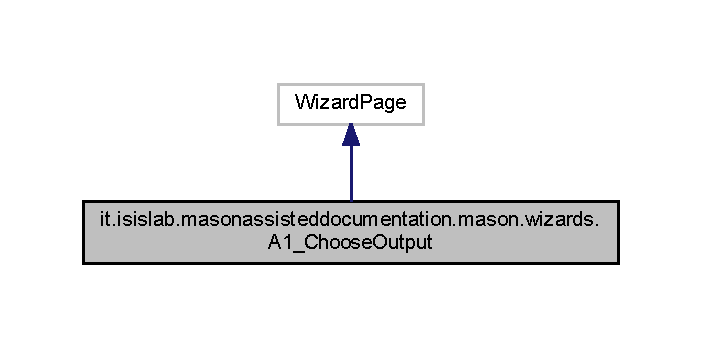
\includegraphics[width=337pt]{classit_1_1isislab_1_1masonassisteddocumentation_1_1mason_1_1wizards_1_1_a1___choose_output__inherit__graph}
\end{center}
\end{figure}


Collaboration diagram for it.\-isislab.\-masonassisteddocumentation.\-mason.\-wizards.\-A1\-\_\-\-Choose\-Output\-:
\nopagebreak
\begin{figure}[H]
\begin{center}
\leavevmode
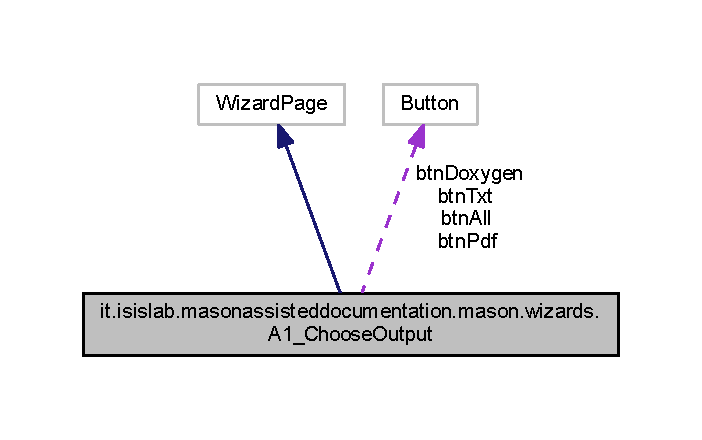
\includegraphics[width=337pt]{classit_1_1isislab_1_1masonassisteddocumentation_1_1mason_1_1wizards_1_1_a1___choose_output__coll__graph}
\end{center}
\end{figure}
\subsection*{Public Member Functions}
\begin{DoxyCompactItemize}
\item 
\hyperlink{classit_1_1isislab_1_1masonassisteddocumentation_1_1mason_1_1wizards_1_1_a1___choose_output_aba04d6e4cd59c54217ea65e4fb06122e}{A1\-\_\-\-Choose\-Output} ()
\item 
void \hyperlink{classit_1_1isislab_1_1masonassisteddocumentation_1_1mason_1_1wizards_1_1_a1___choose_output_a9f06e01c71cae4b98c300170ab2515a5}{create\-Control} (Composite parent)
\item 
I\-Wizard\-Page \hyperlink{classit_1_1isislab_1_1masonassisteddocumentation_1_1mason_1_1wizards_1_1_a1___choose_output_aec3a9e606237eb3fc60b7936749fc91e}{get\-Next\-Page} ()
\end{DoxyCompactItemize}
\subsection*{Package Attributes}
\begin{DoxyCompactItemize}
\item 
Button \hyperlink{classit_1_1isislab_1_1masonassisteddocumentation_1_1mason_1_1wizards_1_1_a1___choose_output_a9b810d24e36dd0e722f76a0f0a9b064b}{btn\-Pdf}
\item 
Button \hyperlink{classit_1_1isislab_1_1masonassisteddocumentation_1_1mason_1_1wizards_1_1_a1___choose_output_a7a3e59d93bfba5d422c70ffdaf34f8ae}{btn\-Txt}
\item 
Button \hyperlink{classit_1_1isislab_1_1masonassisteddocumentation_1_1mason_1_1wizards_1_1_a1___choose_output_aebfe811a15807a6648df6d7cb9ce1196}{btn\-All}
\end{DoxyCompactItemize}
\subsection*{Private Member Functions}
\begin{DoxyCompactItemize}
\item 
void \hyperlink{classit_1_1isislab_1_1masonassisteddocumentation_1_1mason_1_1wizards_1_1_a1___choose_output_a4602f301eef9ed9fbb73ef78b00ae401}{set\-Selected} ()
\end{DoxyCompactItemize}
\subsection*{Private Attributes}
\begin{DoxyCompactItemize}
\item 
Button \hyperlink{classit_1_1isislab_1_1masonassisteddocumentation_1_1mason_1_1wizards_1_1_a1___choose_output_a64285d7a7afd8d13b8da8dfc76d8c524}{btn\-Doxygen}
\end{DoxyCompactItemize}


\subsection{Constructor \& Destructor Documentation}
\hypertarget{classit_1_1isislab_1_1masonassisteddocumentation_1_1mason_1_1wizards_1_1_a1___choose_output_aba04d6e4cd59c54217ea65e4fb06122e}{\index{it\-::isislab\-::masonassisteddocumentation\-::mason\-::wizards\-::\-A1\-\_\-\-Choose\-Output@{it\-::isislab\-::masonassisteddocumentation\-::mason\-::wizards\-::\-A1\-\_\-\-Choose\-Output}!A1\-\_\-\-Choose\-Output@{A1\-\_\-\-Choose\-Output}}
\index{A1\-\_\-\-Choose\-Output@{A1\-\_\-\-Choose\-Output}!it::isislab::masonassisteddocumentation::mason::wizards::A1_ChooseOutput@{it\-::isislab\-::masonassisteddocumentation\-::mason\-::wizards\-::\-A1\-\_\-\-Choose\-Output}}
\subsubsection[{A1\-\_\-\-Choose\-Output}]{\setlength{\rightskip}{0pt plus 5cm}it.\-isislab.\-masonassisteddocumentation.\-mason.\-wizards.\-A1\-\_\-\-Choose\-Output.\-A1\-\_\-\-Choose\-Output (
\begin{DoxyParamCaption}
{}
\end{DoxyParamCaption}
)}}\label{classit_1_1isislab_1_1masonassisteddocumentation_1_1mason_1_1wizards_1_1_a1___choose_output_aba04d6e4cd59c54217ea65e4fb06122e}
Create the wizard. 
\begin{DoxyCode}
20                              \{
21         super(\textcolor{stringliteral}{"wizardPage"});
22         setTitle(\textcolor{stringliteral}{"Output"});
23         setDescription(\textcolor{stringliteral}{"Choose output format"});
24     \}
\end{DoxyCode}


\subsection{Member Function Documentation}
\hypertarget{classit_1_1isislab_1_1masonassisteddocumentation_1_1mason_1_1wizards_1_1_a1___choose_output_a9f06e01c71cae4b98c300170ab2515a5}{\index{it\-::isislab\-::masonassisteddocumentation\-::mason\-::wizards\-::\-A1\-\_\-\-Choose\-Output@{it\-::isislab\-::masonassisteddocumentation\-::mason\-::wizards\-::\-A1\-\_\-\-Choose\-Output}!create\-Control@{create\-Control}}
\index{create\-Control@{create\-Control}!it::isislab::masonassisteddocumentation::mason::wizards::A1_ChooseOutput@{it\-::isislab\-::masonassisteddocumentation\-::mason\-::wizards\-::\-A1\-\_\-\-Choose\-Output}}
\subsubsection[{create\-Control}]{\setlength{\rightskip}{0pt plus 5cm}void it.\-isislab.\-masonassisteddocumentation.\-mason.\-wizards.\-A1\-\_\-\-Choose\-Output.\-create\-Control (
\begin{DoxyParamCaption}
\item[{Composite}]{parent}
\end{DoxyParamCaption}
)}}\label{classit_1_1isislab_1_1masonassisteddocumentation_1_1mason_1_1wizards_1_1_a1___choose_output_a9f06e01c71cae4b98c300170ab2515a5}
Create contents of the wizard. 
\begin{DoxyParams}{Parameters}
{\em parent} & \\
\hline
\end{DoxyParams}

\begin{DoxyCode}
30                                                 \{
31         Composite container = \textcolor{keyword}{new} Composite(parent, SWT.NULL);
32 
33         setControl(container);
34         container.setLayout(\textcolor{keyword}{new} GridLayout(3, \textcolor{keyword}{false}));
35         \textcolor{keyword}{new} Label(container, SWT.NONE);
36         \textcolor{keyword}{new} Label(container, SWT.NONE);
37         \textcolor{keyword}{new} Label(container, SWT.NONE);
38         \textcolor{keyword}{new} Label(container, SWT.NONE);
39         
40         \hyperlink{classit_1_1isislab_1_1masonassisteddocumentation_1_1mason_1_1wizards_1_1_a1___choose_output_a64285d7a7afd8d13b8da8dfc76d8c524}{btnDoxygen} = \textcolor{keyword}{new} Button(container, SWT.RADIO);
41         btnDoxygen.addSelectionListener(\textcolor{keyword}{new} SelectionAdapter() \{
42             @Override
43             \textcolor{keyword}{public} \textcolor{keywordtype}{void} widgetSelected(SelectionEvent e) \{
44                 ConfigFile.setProperty(\textcolor{stringliteral}{"typeOutput"}, \textcolor{stringliteral}{"Doxygen"});
45             \}
46         \});
47         btnDoxygen.setText(\textcolor{stringliteral}{"Doxygen"});
48         
49         Label lblNewLabel = \textcolor{keyword}{new} Label(container, SWT.NONE);
50         lblNewLabel.setText(\textcolor{stringliteral}{"This require Doxygen installation. Output will contain html and latex."});
51         \textcolor{keyword}{new} Label(container, SWT.NONE);
52         \textcolor{keyword}{new} Label(container, SWT.NONE);
53         \textcolor{keyword}{new} Label(container, SWT.NONE);
54         \textcolor{keyword}{new} Label(container, SWT.NONE);
55         
56         \hyperlink{classit_1_1isislab_1_1masonassisteddocumentation_1_1mason_1_1wizards_1_1_a1___choose_output_a9b810d24e36dd0e722f76a0f0a9b064b}{btnPdf} = \textcolor{keyword}{new} Button(container, SWT.RADIO);
57         btnPdf.addSelectionListener(\textcolor{keyword}{new} SelectionAdapter() \{
58             @Override
59             \textcolor{keyword}{public} \textcolor{keywordtype}{void} widgetSelected(SelectionEvent e) \{
60                 ConfigFile.setProperty(\textcolor{stringliteral}{"typeOutput"}, \textcolor{stringliteral}{"pdf"});
61             \}
62         \});
63         btnPdf.setText(\textcolor{stringliteral}{"pdf-rtf"});
64         
65         Label lblThisChooiseWill = \textcolor{keyword}{new} Label(container, SWT.NONE);
66         lblThisChooiseWill.setText(\textcolor{stringliteral}{"This choise will generate pdf and rtf documents."});
67         \textcolor{keyword}{new} Label(container, SWT.NONE);
68         \textcolor{keyword}{new} Label(container, SWT.NONE);
69         \textcolor{keyword}{new} Label(container, SWT.NONE);
70         \textcolor{keyword}{new} Label(container, SWT.NONE);
71         
72         \hyperlink{classit_1_1isislab_1_1masonassisteddocumentation_1_1mason_1_1wizards_1_1_a1___choose_output_a7a3e59d93bfba5d422c70ffdaf34f8ae}{btnTxt} = \textcolor{keyword}{new} Button(container, SWT.RADIO);
73         btnTxt.addSelectionListener(\textcolor{keyword}{new} SelectionAdapter() \{
74             @Override
75             \textcolor{keyword}{public} \textcolor{keywordtype}{void} widgetSelected(SelectionEvent e) \{
76                 ConfigFile.setProperty(\textcolor{stringliteral}{"typeOutput"}, \textcolor{stringliteral}{"txt"});
77             \}
78         \});
79         btnTxt.setText(\textcolor{stringliteral}{"txt"});
80         
81         Label lblThisChooseWill = \textcolor{keyword}{new} Label(container, SWT.NONE);
82         lblThisChooseWill.setText(\textcolor{stringliteral}{"This choise will generate a txt document."});
83         \textcolor{keyword}{new} Label(container, SWT.NONE);
84         \textcolor{keyword}{new} Label(container, SWT.NONE);
85         \textcolor{keyword}{new} Label(container, SWT.NONE);
86         \textcolor{keyword}{new} Label(container, SWT.NONE);
87         
88         \hyperlink{classit_1_1isislab_1_1masonassisteddocumentation_1_1mason_1_1wizards_1_1_a1___choose_output_aebfe811a15807a6648df6d7cb9ce1196}{btnAll} = \textcolor{keyword}{new} Button(container, SWT.RADIO);
89         btnAll.addSelectionListener(\textcolor{keyword}{new} SelectionAdapter() \{
90             @Override
91             \textcolor{keyword}{public} \textcolor{keywordtype}{void} widgetSelected(SelectionEvent e) \{
92                 ConfigFile.setProperty(\textcolor{stringliteral}{"typeOutput"}, \textcolor{stringliteral}{"all"});
93             \}
94         \});
95         btnAll.setText(\textcolor{stringliteral}{"All"});
96         
97         \hyperlink{classit_1_1isislab_1_1masonassisteddocumentation_1_1mason_1_1wizards_1_1_a1___choose_output_a4602f301eef9ed9fbb73ef78b00ae401}{setSelected}();
98         
99         Label labelAll = \textcolor{keyword}{new} Label(container, SWT.NONE);
100         labelAll.setText(\textcolor{stringliteral}{"This choise will generate html-latex(with Doxygen), pdf-rtf and txt."});
101     \}
\end{DoxyCode}


Here is the call graph for this function\-:
\nopagebreak
\begin{figure}[H]
\begin{center}
\leavevmode
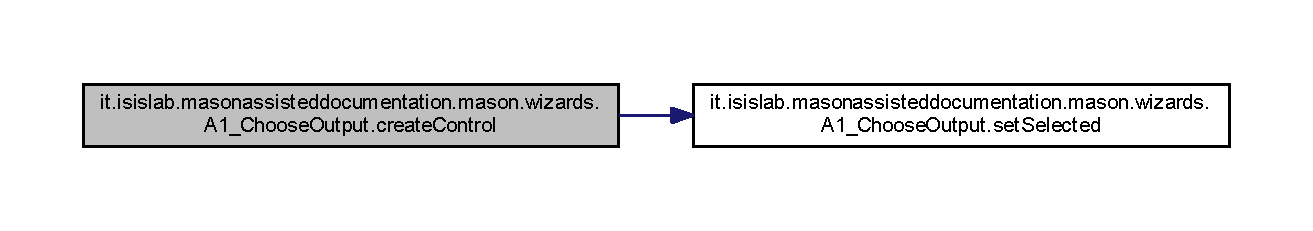
\includegraphics[width=350pt]{classit_1_1isislab_1_1masonassisteddocumentation_1_1mason_1_1wizards_1_1_a1___choose_output_a9f06e01c71cae4b98c300170ab2515a5_cgraph}
\end{center}
\end{figure}


\hypertarget{classit_1_1isislab_1_1masonassisteddocumentation_1_1mason_1_1wizards_1_1_a1___choose_output_aec3a9e606237eb3fc60b7936749fc91e}{\index{it\-::isislab\-::masonassisteddocumentation\-::mason\-::wizards\-::\-A1\-\_\-\-Choose\-Output@{it\-::isislab\-::masonassisteddocumentation\-::mason\-::wizards\-::\-A1\-\_\-\-Choose\-Output}!get\-Next\-Page@{get\-Next\-Page}}
\index{get\-Next\-Page@{get\-Next\-Page}!it::isislab::masonassisteddocumentation::mason::wizards::A1_ChooseOutput@{it\-::isislab\-::masonassisteddocumentation\-::mason\-::wizards\-::\-A1\-\_\-\-Choose\-Output}}
\subsubsection[{get\-Next\-Page}]{\setlength{\rightskip}{0pt plus 5cm}I\-Wizard\-Page it.\-isislab.\-masonassisteddocumentation.\-mason.\-wizards.\-A1\-\_\-\-Choose\-Output.\-get\-Next\-Page (
\begin{DoxyParamCaption}
{}
\end{DoxyParamCaption}
)}}\label{classit_1_1isislab_1_1masonassisteddocumentation_1_1mason_1_1wizards_1_1_a1___choose_output_aec3a9e606237eb3fc60b7936749fc91e}

\begin{DoxyCode}
113                                     \{ 
114         \textcolor{keywordflow}{if} (\hyperlink{classit_1_1isislab_1_1masonassisteddocumentation_1_1mason_1_1wizards_1_1_a1___choose_output_a64285d7a7afd8d13b8da8dfc76d8c524}{btnDoxygen}.getSelection())    ConfigFile.setProperty(\textcolor{stringliteral}{"typeOutput"}, \textcolor{stringliteral}{"Doxygen"});
115         \textcolor{keywordflow}{if} (\hyperlink{classit_1_1isislab_1_1masonassisteddocumentation_1_1mason_1_1wizards_1_1_a1___choose_output_a9b810d24e36dd0e722f76a0f0a9b064b}{btnPdf}.getSelection())    ConfigFile.setProperty(\textcolor{stringliteral}{"typeOutput"}, \textcolor{stringliteral}{"pdf"});
116         \textcolor{keywordflow}{if} (\hyperlink{classit_1_1isislab_1_1masonassisteddocumentation_1_1mason_1_1wizards_1_1_a1___choose_output_a7a3e59d93bfba5d422c70ffdaf34f8ae}{btnTxt}.getSelection())    ConfigFile.setProperty(\textcolor{stringliteral}{"typeOutput"}, \textcolor{stringliteral}{"txt"});
117         \textcolor{keywordflow}{if} (\hyperlink{classit_1_1isislab_1_1masonassisteddocumentation_1_1mason_1_1wizards_1_1_a1___choose_output_aebfe811a15807a6648df6d7cb9ce1196}{btnAll}.getSelection())    ConfigFile.setProperty(\textcolor{stringliteral}{"typeOutput"}, \textcolor{stringliteral}{"all"});
118         
119         B\_ProjectInformationPage nextPage = \textcolor{keyword}{new} B\_ProjectInformationPage();
120         ((MASONDocumentationWizard) super.getWizard()).addPage(nextPage);
121         \textcolor{keywordflow}{return} nextPage;
122     \}
\end{DoxyCode}


Here is the call graph for this function\-:
\nopagebreak
\begin{figure}[H]
\begin{center}
\leavevmode
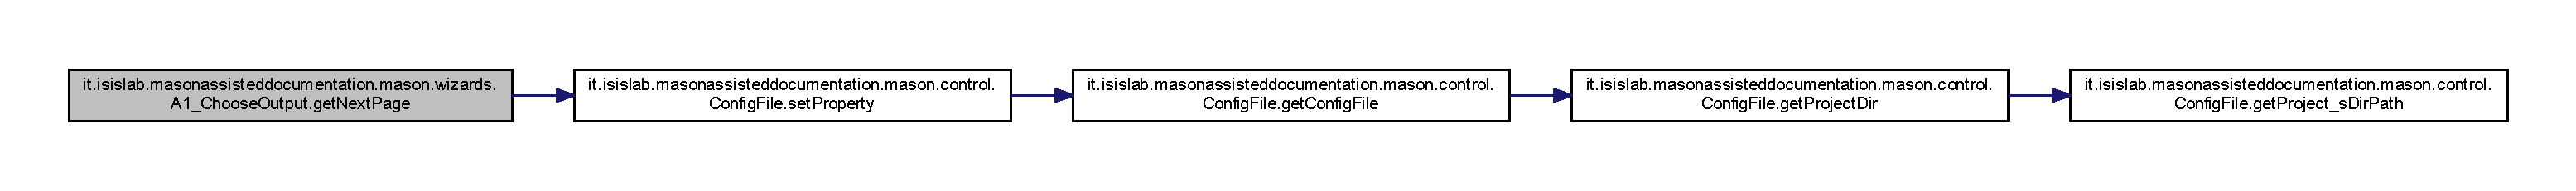
\includegraphics[width=350pt]{classit_1_1isislab_1_1masonassisteddocumentation_1_1mason_1_1wizards_1_1_a1___choose_output_aec3a9e606237eb3fc60b7936749fc91e_cgraph}
\end{center}
\end{figure}


\hypertarget{classit_1_1isislab_1_1masonassisteddocumentation_1_1mason_1_1wizards_1_1_a1___choose_output_a4602f301eef9ed9fbb73ef78b00ae401}{\index{it\-::isislab\-::masonassisteddocumentation\-::mason\-::wizards\-::\-A1\-\_\-\-Choose\-Output@{it\-::isislab\-::masonassisteddocumentation\-::mason\-::wizards\-::\-A1\-\_\-\-Choose\-Output}!set\-Selected@{set\-Selected}}
\index{set\-Selected@{set\-Selected}!it::isislab::masonassisteddocumentation::mason::wizards::A1_ChooseOutput@{it\-::isislab\-::masonassisteddocumentation\-::mason\-::wizards\-::\-A1\-\_\-\-Choose\-Output}}
\subsubsection[{set\-Selected}]{\setlength{\rightskip}{0pt plus 5cm}void it.\-isislab.\-masonassisteddocumentation.\-mason.\-wizards.\-A1\-\_\-\-Choose\-Output.\-set\-Selected (
\begin{DoxyParamCaption}
{}
\end{DoxyParamCaption}
)\hspace{0.3cm}{\ttfamily [private]}}}\label{classit_1_1isislab_1_1masonassisteddocumentation_1_1mason_1_1wizards_1_1_a1___choose_output_a4602f301eef9ed9fbb73ef78b00ae401}

\begin{DoxyCode}
103                                \{
104         String typeOutput = ConfigFile.getValue(\textcolor{stringliteral}{"typeOutput"});
105         \textcolor{keywordflow}{if} (typeOutput.equals(\textcolor{stringliteral}{"Doxygen"}))   \hyperlink{classit_1_1isislab_1_1masonassisteddocumentation_1_1mason_1_1wizards_1_1_a1___choose_output_a64285d7a7afd8d13b8da8dfc76d8c524}{btnDoxygen}.setSelection(\textcolor{keyword}{true});
106         \textcolor{keywordflow}{else} \textcolor{keywordflow}{if} (typeOutput.equals(\textcolor{stringliteral}{"pdf"}))  \hyperlink{classit_1_1isislab_1_1masonassisteddocumentation_1_1mason_1_1wizards_1_1_a1___choose_output_a9b810d24e36dd0e722f76a0f0a9b064b}{btnPdf}.setSelection(\textcolor{keyword}{true});
107         \textcolor{keywordflow}{else} \textcolor{keywordflow}{if} (typeOutput.equals(\textcolor{stringliteral}{"txt"}))  \hyperlink{classit_1_1isislab_1_1masonassisteddocumentation_1_1mason_1_1wizards_1_1_a1___choose_output_a7a3e59d93bfba5d422c70ffdaf34f8ae}{btnTxt}.setSelection(\textcolor{keyword}{true});
108         \textcolor{keywordflow}{else} \textcolor{keywordflow}{if} (typeOutput.equals(\textcolor{stringliteral}{"all"}))  \hyperlink{classit_1_1isislab_1_1masonassisteddocumentation_1_1mason_1_1wizards_1_1_a1___choose_output_aebfe811a15807a6648df6d7cb9ce1196}{btnAll}.setSelection(\textcolor{keyword}{true});
109         \textcolor{keywordflow}{else}
110             btnDoxygen.setSelection(\textcolor{keyword}{true});
111     \}
\end{DoxyCode}


Here is the caller graph for this function\-:
\nopagebreak
\begin{figure}[H]
\begin{center}
\leavevmode
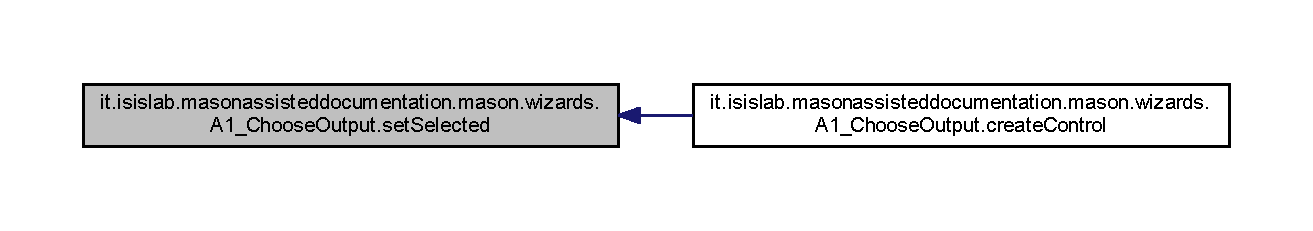
\includegraphics[width=350pt]{classit_1_1isislab_1_1masonassisteddocumentation_1_1mason_1_1wizards_1_1_a1___choose_output_a4602f301eef9ed9fbb73ef78b00ae401_icgraph}
\end{center}
\end{figure}




\subsection{Member Data Documentation}
\hypertarget{classit_1_1isislab_1_1masonassisteddocumentation_1_1mason_1_1wizards_1_1_a1___choose_output_aebfe811a15807a6648df6d7cb9ce1196}{\index{it\-::isislab\-::masonassisteddocumentation\-::mason\-::wizards\-::\-A1\-\_\-\-Choose\-Output@{it\-::isislab\-::masonassisteddocumentation\-::mason\-::wizards\-::\-A1\-\_\-\-Choose\-Output}!btn\-All@{btn\-All}}
\index{btn\-All@{btn\-All}!it::isislab::masonassisteddocumentation::mason::wizards::A1_ChooseOutput@{it\-::isislab\-::masonassisteddocumentation\-::mason\-::wizards\-::\-A1\-\_\-\-Choose\-Output}}
\subsubsection[{btn\-All}]{\setlength{\rightskip}{0pt plus 5cm}Button it.\-isislab.\-masonassisteddocumentation.\-mason.\-wizards.\-A1\-\_\-\-Choose\-Output.\-btn\-All\hspace{0.3cm}{\ttfamily [package]}}}\label{classit_1_1isislab_1_1masonassisteddocumentation_1_1mason_1_1wizards_1_1_a1___choose_output_aebfe811a15807a6648df6d7cb9ce1196}
\hypertarget{classit_1_1isislab_1_1masonassisteddocumentation_1_1mason_1_1wizards_1_1_a1___choose_output_a64285d7a7afd8d13b8da8dfc76d8c524}{\index{it\-::isislab\-::masonassisteddocumentation\-::mason\-::wizards\-::\-A1\-\_\-\-Choose\-Output@{it\-::isislab\-::masonassisteddocumentation\-::mason\-::wizards\-::\-A1\-\_\-\-Choose\-Output}!btn\-Doxygen@{btn\-Doxygen}}
\index{btn\-Doxygen@{btn\-Doxygen}!it::isislab::masonassisteddocumentation::mason::wizards::A1_ChooseOutput@{it\-::isislab\-::masonassisteddocumentation\-::mason\-::wizards\-::\-A1\-\_\-\-Choose\-Output}}
\subsubsection[{btn\-Doxygen}]{\setlength{\rightskip}{0pt plus 5cm}Button it.\-isislab.\-masonassisteddocumentation.\-mason.\-wizards.\-A1\-\_\-\-Choose\-Output.\-btn\-Doxygen\hspace{0.3cm}{\ttfamily [private]}}}\label{classit_1_1isislab_1_1masonassisteddocumentation_1_1mason_1_1wizards_1_1_a1___choose_output_a64285d7a7afd8d13b8da8dfc76d8c524}
\hypertarget{classit_1_1isislab_1_1masonassisteddocumentation_1_1mason_1_1wizards_1_1_a1___choose_output_a9b810d24e36dd0e722f76a0f0a9b064b}{\index{it\-::isislab\-::masonassisteddocumentation\-::mason\-::wizards\-::\-A1\-\_\-\-Choose\-Output@{it\-::isislab\-::masonassisteddocumentation\-::mason\-::wizards\-::\-A1\-\_\-\-Choose\-Output}!btn\-Pdf@{btn\-Pdf}}
\index{btn\-Pdf@{btn\-Pdf}!it::isislab::masonassisteddocumentation::mason::wizards::A1_ChooseOutput@{it\-::isislab\-::masonassisteddocumentation\-::mason\-::wizards\-::\-A1\-\_\-\-Choose\-Output}}
\subsubsection[{btn\-Pdf}]{\setlength{\rightskip}{0pt plus 5cm}Button it.\-isislab.\-masonassisteddocumentation.\-mason.\-wizards.\-A1\-\_\-\-Choose\-Output.\-btn\-Pdf\hspace{0.3cm}{\ttfamily [package]}}}\label{classit_1_1isislab_1_1masonassisteddocumentation_1_1mason_1_1wizards_1_1_a1___choose_output_a9b810d24e36dd0e722f76a0f0a9b064b}
\hypertarget{classit_1_1isislab_1_1masonassisteddocumentation_1_1mason_1_1wizards_1_1_a1___choose_output_a7a3e59d93bfba5d422c70ffdaf34f8ae}{\index{it\-::isislab\-::masonassisteddocumentation\-::mason\-::wizards\-::\-A1\-\_\-\-Choose\-Output@{it\-::isislab\-::masonassisteddocumentation\-::mason\-::wizards\-::\-A1\-\_\-\-Choose\-Output}!btn\-Txt@{btn\-Txt}}
\index{btn\-Txt@{btn\-Txt}!it::isislab::masonassisteddocumentation::mason::wizards::A1_ChooseOutput@{it\-::isislab\-::masonassisteddocumentation\-::mason\-::wizards\-::\-A1\-\_\-\-Choose\-Output}}
\subsubsection[{btn\-Txt}]{\setlength{\rightskip}{0pt plus 5cm}Button it.\-isislab.\-masonassisteddocumentation.\-mason.\-wizards.\-A1\-\_\-\-Choose\-Output.\-btn\-Txt\hspace{0.3cm}{\ttfamily [package]}}}\label{classit_1_1isislab_1_1masonassisteddocumentation_1_1mason_1_1wizards_1_1_a1___choose_output_a7a3e59d93bfba5d422c70ffdaf34f8ae}


The documentation for this class was generated from the following file\-:\begin{DoxyCompactItemize}
\item 
src/it/isislab/masonassisteddocumentation/mason/wizards/\hyperlink{_a1___choose_output_8java}{A1\-\_\-\-Choose\-Output.\-java}\end{DoxyCompactItemize}

\hypertarget{classit_1_1isislab_1_1masonassisteddocumentation_1_1mason_1_1wizards_1_1_a___introduction_page}{\section{it.\-isislab.\-masonassisteddocumentation.\-mason.\-wizards.\-A\-\_\-\-Introduction\-Page Class Reference}
\label{classit_1_1isislab_1_1masonassisteddocumentation_1_1mason_1_1wizards_1_1_a___introduction_page}\index{it.\-isislab.\-masonassisteddocumentation.\-mason.\-wizards.\-A\-\_\-\-Introduction\-Page@{it.\-isislab.\-masonassisteddocumentation.\-mason.\-wizards.\-A\-\_\-\-Introduction\-Page}}
}


Inheritance diagram for it.\-isislab.\-masonassisteddocumentation.\-mason.\-wizards.\-A\-\_\-\-Introduction\-Page\-:\nopagebreak
\begin{figure}[H]
\begin{center}
\leavevmode
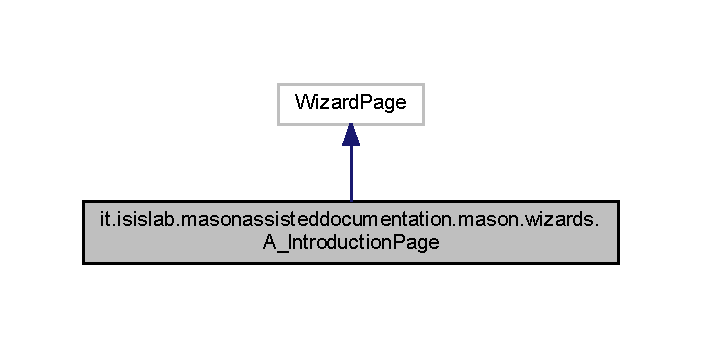
\includegraphics[width=337pt]{classit_1_1isislab_1_1masonassisteddocumentation_1_1mason_1_1wizards_1_1_a___introduction_page__inherit__graph}
\end{center}
\end{figure}


Collaboration diagram for it.\-isislab.\-masonassisteddocumentation.\-mason.\-wizards.\-A\-\_\-\-Introduction\-Page\-:\nopagebreak
\begin{figure}[H]
\begin{center}
\leavevmode
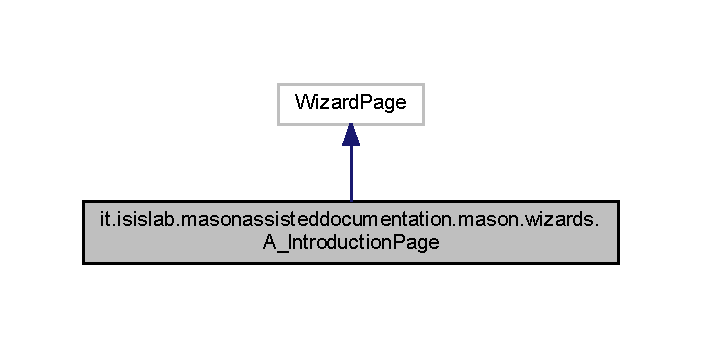
\includegraphics[width=337pt]{classit_1_1isislab_1_1masonassisteddocumentation_1_1mason_1_1wizards_1_1_a___introduction_page__coll__graph}
\end{center}
\end{figure}
\subsection*{Public Member Functions}
\begin{DoxyCompactItemize}
\item 
\hyperlink{classit_1_1isislab_1_1masonassisteddocumentation_1_1mason_1_1wizards_1_1_a___introduction_page_afa9c82287e69bc1268264bba861a56d1}{A\-\_\-\-Introduction\-Page} ()
\item 
void \hyperlink{classit_1_1isislab_1_1masonassisteddocumentation_1_1mason_1_1wizards_1_1_a___introduction_page_a18a66da4d6393cfb232dd2d550eb2d9c}{create\-Control} (Composite parent)
\item 
I\-Wizard\-Page \hyperlink{classit_1_1isislab_1_1masonassisteddocumentation_1_1mason_1_1wizards_1_1_a___introduction_page_a1667a8d8ef50454c7a79c956f8f6fafb}{get\-Next\-Page} ()
\end{DoxyCompactItemize}
\subsection*{Static Private Attributes}
\begin{DoxyCompactItemize}
\item 
static String \hyperlink{classit_1_1isislab_1_1masonassisteddocumentation_1_1mason_1_1wizards_1_1_a___introduction_page_a2b1741f1921be08167b8d766305b1161}{introduction}
\end{DoxyCompactItemize}


\subsection{Constructor \& Destructor Documentation}
\hypertarget{classit_1_1isislab_1_1masonassisteddocumentation_1_1mason_1_1wizards_1_1_a___introduction_page_afa9c82287e69bc1268264bba861a56d1}{\index{it\-::isislab\-::masonassisteddocumentation\-::mason\-::wizards\-::\-A\-\_\-\-Introduction\-Page@{it\-::isislab\-::masonassisteddocumentation\-::mason\-::wizards\-::\-A\-\_\-\-Introduction\-Page}!A\-\_\-\-Introduction\-Page@{A\-\_\-\-Introduction\-Page}}
\index{A\-\_\-\-Introduction\-Page@{A\-\_\-\-Introduction\-Page}!it::isislab::masonassisteddocumentation::mason::wizards::A_IntroductionPage@{it\-::isislab\-::masonassisteddocumentation\-::mason\-::wizards\-::\-A\-\_\-\-Introduction\-Page}}
\subsubsection[{A\-\_\-\-Introduction\-Page}]{\setlength{\rightskip}{0pt plus 5cm}it.\-isislab.\-masonassisteddocumentation.\-mason.\-wizards.\-A\-\_\-\-Introduction\-Page.\-A\-\_\-\-Introduction\-Page (
\begin{DoxyParamCaption}
{}
\end{DoxyParamCaption}
)}}\label{classit_1_1isislab_1_1masonassisteddocumentation_1_1mason_1_1wizards_1_1_a___introduction_page_afa9c82287e69bc1268264bba861a56d1}
Create the wizard. 
\begin{DoxyCode}
29                                 \{
30         super(\textcolor{stringliteral}{"wizardPage"});
31         setTitle(\textcolor{stringliteral}{"ABMs ODD documentation"});
32         setDescription(\textcolor{stringliteral}{"Welcome to ABMs ODD wizard"});
33     \}
\end{DoxyCode}


\subsection{Member Function Documentation}
\hypertarget{classit_1_1isislab_1_1masonassisteddocumentation_1_1mason_1_1wizards_1_1_a___introduction_page_a18a66da4d6393cfb232dd2d550eb2d9c}{\index{it\-::isislab\-::masonassisteddocumentation\-::mason\-::wizards\-::\-A\-\_\-\-Introduction\-Page@{it\-::isislab\-::masonassisteddocumentation\-::mason\-::wizards\-::\-A\-\_\-\-Introduction\-Page}!create\-Control@{create\-Control}}
\index{create\-Control@{create\-Control}!it::isislab::masonassisteddocumentation::mason::wizards::A_IntroductionPage@{it\-::isislab\-::masonassisteddocumentation\-::mason\-::wizards\-::\-A\-\_\-\-Introduction\-Page}}
\subsubsection[{create\-Control}]{\setlength{\rightskip}{0pt plus 5cm}void it.\-isislab.\-masonassisteddocumentation.\-mason.\-wizards.\-A\-\_\-\-Introduction\-Page.\-create\-Control (
\begin{DoxyParamCaption}
\item[{Composite}]{parent}
\end{DoxyParamCaption}
)}}\label{classit_1_1isislab_1_1masonassisteddocumentation_1_1mason_1_1wizards_1_1_a___introduction_page_a18a66da4d6393cfb232dd2d550eb2d9c}
Create contents of the wizard. 
\begin{DoxyParams}{Parameters}
{\em parent} & \\
\hline
\end{DoxyParams}

\begin{DoxyCode}
39                                                 \{
40         Composite container = \textcolor{keyword}{new} Composite(parent, SWT.NONE);
41 
42         setControl(container);
43         
44         Label lblIntroduction = \textcolor{keyword}{new} Label(container, SWT.NONE);
45         lblIntroduction.setBounds(10, 10, 554, 189);
46         lblIntroduction.setText(\hyperlink{classit_1_1isislab_1_1masonassisteddocumentation_1_1mason_1_1wizards_1_1_a___introduction_page_a2b1741f1921be08167b8d766305b1161}{introduction});
47     \}
\end{DoxyCode}
\hypertarget{classit_1_1isislab_1_1masonassisteddocumentation_1_1mason_1_1wizards_1_1_a___introduction_page_a1667a8d8ef50454c7a79c956f8f6fafb}{\index{it\-::isislab\-::masonassisteddocumentation\-::mason\-::wizards\-::\-A\-\_\-\-Introduction\-Page@{it\-::isislab\-::masonassisteddocumentation\-::mason\-::wizards\-::\-A\-\_\-\-Introduction\-Page}!get\-Next\-Page@{get\-Next\-Page}}
\index{get\-Next\-Page@{get\-Next\-Page}!it::isislab::masonassisteddocumentation::mason::wizards::A_IntroductionPage@{it\-::isislab\-::masonassisteddocumentation\-::mason\-::wizards\-::\-A\-\_\-\-Introduction\-Page}}
\subsubsection[{get\-Next\-Page}]{\setlength{\rightskip}{0pt plus 5cm}I\-Wizard\-Page it.\-isislab.\-masonassisteddocumentation.\-mason.\-wizards.\-A\-\_\-\-Introduction\-Page.\-get\-Next\-Page (
\begin{DoxyParamCaption}
{}
\end{DoxyParamCaption}
)}}\label{classit_1_1isislab_1_1masonassisteddocumentation_1_1mason_1_1wizards_1_1_a___introduction_page_a1667a8d8ef50454c7a79c956f8f6fafb}

\begin{DoxyCode}
49                                     \{ 
50         A1\_ChooseOutput nextPage = \textcolor{keyword}{new} A1\_ChooseOutput();
51         ((MASONDocumentationWizard) super.getWizard()).addPage(nextPage);
52         \textcolor{keywordflow}{return} nextPage;
53     \}
\end{DoxyCode}


\subsection{Member Data Documentation}
\hypertarget{classit_1_1isislab_1_1masonassisteddocumentation_1_1mason_1_1wizards_1_1_a___introduction_page_a2b1741f1921be08167b8d766305b1161}{\index{it\-::isislab\-::masonassisteddocumentation\-::mason\-::wizards\-::\-A\-\_\-\-Introduction\-Page@{it\-::isislab\-::masonassisteddocumentation\-::mason\-::wizards\-::\-A\-\_\-\-Introduction\-Page}!introduction@{introduction}}
\index{introduction@{introduction}!it::isislab::masonassisteddocumentation::mason::wizards::A_IntroductionPage@{it\-::isislab\-::masonassisteddocumentation\-::mason\-::wizards\-::\-A\-\_\-\-Introduction\-Page}}
\subsubsection[{introduction}]{\setlength{\rightskip}{0pt plus 5cm}String it.\-isislab.\-masonassisteddocumentation.\-mason.\-wizards.\-A\-\_\-\-Introduction\-Page.\-introduction\hspace{0.3cm}{\ttfamily [static]}, {\ttfamily [private]}}}\label{classit_1_1isislab_1_1masonassisteddocumentation_1_1mason_1_1wizards_1_1_a___introduction_page_a2b1741f1921be08167b8d766305b1161}
{\bfseries Initial value\-:}
\begin{DoxyCode}
= \textcolor{stringliteral}{"This wizard will auto-generate ABMs "}
                            + \textcolor{stringliteral}{"documentation with the standard ODD format. The objectives of \(\backslash\)n"}
                            + \textcolor{stringliteral}{"ODD are to make model descriptions more understandable and "}
                            + \textcolor{stringliteral}{"complete, thereby making ABMs less \(\backslash\)nsubject to criticism for "}
                            + \textcolor{stringliteral}{"being irreproducible.\(\backslash\)n\(\backslash\)n"}
                            + \textcolor{stringliteral}{"Elements of ODD:\(\backslash\)n"}
                            + \textcolor{stringliteral}{"   1. Purpose\(\backslash\)n"}
                            + \textcolor{stringliteral}{"   2. Entities, state variables, and scales\(\backslash\)n"}
                            + \textcolor{stringliteral}{"   3. Process overview and scheduling\(\backslash\)n"}
                            + \textcolor{stringliteral}{"   4. Design concepts\(\backslash\)n"}
                            + \textcolor{stringliteral}{"   5. Initialization\(\backslash\)n"}  
                            + \textcolor{stringliteral}{"   6. Input data\(\backslash\)n"}
                            + \textcolor{stringliteral}{"   7. Submodels"}
\end{DoxyCode}


The documentation for this class was generated from the following file\-:\begin{DoxyCompactItemize}
\item 
src/it/isislab/masonassisteddocumentation/mason/wizards/\hyperlink{_a___introduction_page_8java}{A\-\_\-\-Introduction\-Page.\-java}\end{DoxyCompactItemize}

\hypertarget{classit_1_1isislab_1_1masonassisteddocumentation_1_1mason_1_1analizer_1_1_agent_analizer}{\section{it.\-isislab.\-masonassisteddocumentation.\-mason.\-analizer.\-Agent\-Analizer Class Reference}
\label{classit_1_1isislab_1_1masonassisteddocumentation_1_1mason_1_1analizer_1_1_agent_analizer}\index{it.\-isislab.\-masonassisteddocumentation.\-mason.\-analizer.\-Agent\-Analizer@{it.\-isislab.\-masonassisteddocumentation.\-mason.\-analizer.\-Agent\-Analizer}}
}


Inheritance diagram for it.\-isislab.\-masonassisteddocumentation.\-mason.\-analizer.\-Agent\-Analizer\-:\nopagebreak
\begin{figure}[H]
\begin{center}
\leavevmode
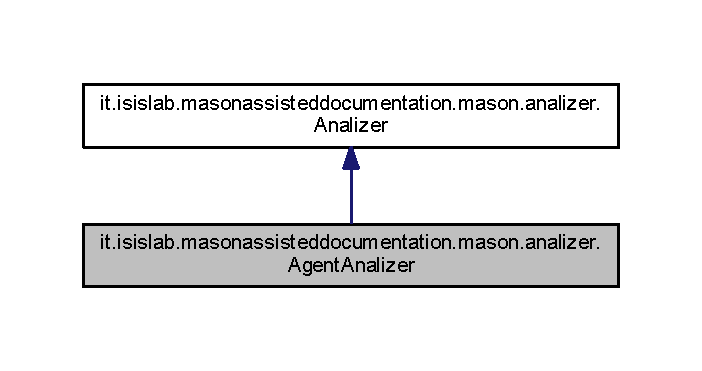
\includegraphics[width=337pt]{classit_1_1isislab_1_1masonassisteddocumentation_1_1mason_1_1analizer_1_1_agent_analizer__inherit__graph}
\end{center}
\end{figure}


Collaboration diagram for it.\-isislab.\-masonassisteddocumentation.\-mason.\-analizer.\-Agent\-Analizer\-:\nopagebreak
\begin{figure}[H]
\begin{center}
\leavevmode
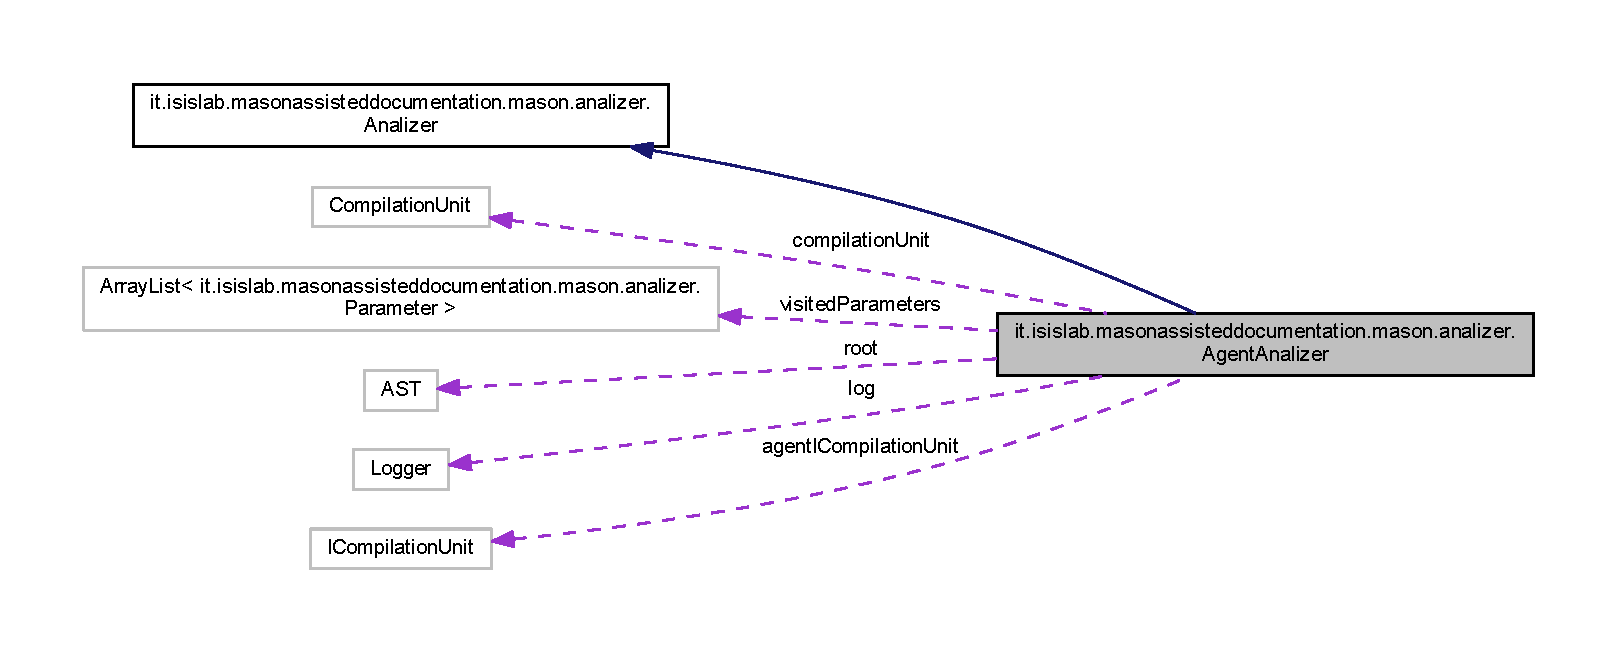
\includegraphics[width=350pt]{classit_1_1isislab_1_1masonassisteddocumentation_1_1mason_1_1analizer_1_1_agent_analizer__coll__graph}
\end{center}
\end{figure}
\subsection*{Public Member Functions}
\begin{DoxyCompactItemize}
\item 
\hyperlink{classit_1_1isislab_1_1masonassisteddocumentation_1_1mason_1_1analizer_1_1_agent_analizer_a73ca1a318ae1635984ceced89e3f8d1d}{Agent\-Analizer} (I\-Compilation\-Unit agent\-C\-U)
\item 
void \hyperlink{classit_1_1isislab_1_1masonassisteddocumentation_1_1mason_1_1analizer_1_1_agent_analizer_aa1cf97eff47c73e305fdd540a512a88c}{rewrite} ()
\item 
void \hyperlink{classit_1_1isislab_1_1masonassisteddocumentation_1_1mason_1_1analizer_1_1_agent_analizer_afd9a63275f03a03ca69187b8cce6613e}{rewrite} (String path\-Name)
\item 
Javadoc \hyperlink{classit_1_1isislab_1_1masonassisteddocumentation_1_1mason_1_1analizer_1_1_agent_analizer_ae8de4d1c4186a27f567257c4b85c3f1c}{get\-Model\-Description} ()
\item 
void \hyperlink{classit_1_1isislab_1_1masonassisteddocumentation_1_1mason_1_1analizer_1_1_agent_analizer_aaef67e385b42699bd863f505be5df17d}{set\-Class\-Description} (String model\-Description)
\item 
Array\-List$<$ \hyperlink{classit_1_1isislab_1_1masonassisteddocumentation_1_1mason_1_1analizer_1_1_parameter}{Parameter} $>$ \hyperlink{classit_1_1isislab_1_1masonassisteddocumentation_1_1mason_1_1analizer_1_1_agent_analizer_a76b619307dd702b85fc422f231fac76a}{get\-Visited\-Parameters} ()
\item 
Array\-List$<$ \hyperlink{classit_1_1isislab_1_1masonassisteddocumentation_1_1mason_1_1analizer_1_1_parameter}{Parameter} $>$ \hyperlink{classit_1_1isislab_1_1masonassisteddocumentation_1_1mason_1_1analizer_1_1_agent_analizer_a351c38491d7f706177c4c76478cabd6d}{get\-Positions\-Parameter} ()
\item 
Compilation\-Unit \hyperlink{classit_1_1isislab_1_1masonassisteddocumentation_1_1mason_1_1analizer_1_1_agent_analizer_a452c584a7035bc8c4a550f4e86db8266}{get\-Compilation\-Unit} ()
\item 
A\-S\-T \hyperlink{classit_1_1isislab_1_1masonassisteddocumentation_1_1mason_1_1analizer_1_1_agent_analizer_a1ac3fc1c6fdf3133e81fba94fe13c01d}{get\-Root} ()
\item 
String \hyperlink{classit_1_1isislab_1_1masonassisteddocumentation_1_1mason_1_1analizer_1_1_agent_analizer_a3e46e6754b6575579be1a9ac062641fa}{get\-Position\-Class} ()
\item 
boolean \hyperlink{classit_1_1isislab_1_1masonassisteddocumentation_1_1mason_1_1analizer_1_1_agent_analizer_a3e5ea2154f20535f5bd33db685cf045c}{already\-Visited} (\hyperlink{classit_1_1isislab_1_1masonassisteddocumentation_1_1mason_1_1analizer_1_1_parameter}{Parameter} p)
\item 
Array\-List$<$ \hyperlink{classit_1_1isislab_1_1masonassisteddocumentation_1_1mason_1_1analizer_1_1_parameter}{Parameter} $>$ \hyperlink{classit_1_1isislab_1_1masonassisteddocumentation_1_1mason_1_1analizer_1_1_agent_analizer_ad237f6e49d6d49e0138b1e2ac6a2b0bb}{get\-Not\-Visited\-Parameter\-\_\-s} ()
\item 
String \hyperlink{classit_1_1isislab_1_1masonassisteddocumentation_1_1mason_1_1analizer_1_1_agent_analizer_a94492199c5e4873a07a2a46d15617937}{get\-Class\-Name} ()
\item 
String \hyperlink{classit_1_1isislab_1_1masonassisteddocumentation_1_1mason_1_1analizer_1_1_agent_analizer_aa1e783609d0c0ffbb244ba4c22abc7b9}{to\-String} ()
\end{DoxyCompactItemize}
\subsection*{Static Public Attributes}
\begin{DoxyCompactItemize}
\item 
static String\mbox{[}$\,$\mbox{]} \hyperlink{classit_1_1isislab_1_1masonassisteddocumentation_1_1mason_1_1analizer_1_1_agent_analizer_aea5eff658e91428950dd0efd1339bf36}{position\-Class} = \{\char`\"{}Int2\-D\char`\"{}, \char`\"{}Double2\-D\char`\"{}, \char`\"{}Int3\-D\char`\"{}, \char`\"{}Double3\-D\char`\"{},\}
\item 
static String \hyperlink{classit_1_1isislab_1_1masonassisteddocumentation_1_1mason_1_1analizer_1_1_agent_analizer_a5c6d63f226ee1dc2a0749c6a5ee40dd9}{steppable\-Description}
\end{DoxyCompactItemize}
\subsection*{Private Attributes}
\begin{DoxyCompactItemize}
\item 
I\-Compilation\-Unit \hyperlink{classit_1_1isislab_1_1masonassisteddocumentation_1_1mason_1_1analizer_1_1_agent_analizer_ab0d7780b5d7b3607251116bf7bcde320}{agent\-I\-Compilation\-Unit}
\item 
Compilation\-Unit \hyperlink{classit_1_1isislab_1_1masonassisteddocumentation_1_1mason_1_1analizer_1_1_agent_analizer_aad9b5d0882694d2802dc24c982f21985}{compilation\-Unit}
\item 
A\-S\-T \hyperlink{classit_1_1isislab_1_1masonassisteddocumentation_1_1mason_1_1analizer_1_1_agent_analizer_a83430d48ecbe1fc48d0cd8f10c2d99a8}{root}
\item 
Array\-List$<$ \hyperlink{classit_1_1isislab_1_1masonassisteddocumentation_1_1mason_1_1analizer_1_1_parameter}{Parameter} $>$ \hyperlink{classit_1_1isislab_1_1masonassisteddocumentation_1_1mason_1_1analizer_1_1_agent_analizer_aee5454eb7063c444081bdb2556d3a60b}{visited\-Parameters}
\end{DoxyCompactItemize}
\subsection*{Static Private Attributes}
\begin{DoxyCompactItemize}
\item 
static Logger \hyperlink{classit_1_1isislab_1_1masonassisteddocumentation_1_1mason_1_1analizer_1_1_agent_analizer_ad9766d313bd07461a473e31b771c26c6}{log} = Logger.\-get\-Logger(\char`\"{}global\char`\"{})
\end{DoxyCompactItemize}


\subsection{Constructor \& Destructor Documentation}
\hypertarget{classit_1_1isislab_1_1masonassisteddocumentation_1_1mason_1_1analizer_1_1_agent_analizer_a73ca1a318ae1635984ceced89e3f8d1d}{\index{it\-::isislab\-::masonassisteddocumentation\-::mason\-::analizer\-::\-Agent\-Analizer@{it\-::isislab\-::masonassisteddocumentation\-::mason\-::analizer\-::\-Agent\-Analizer}!Agent\-Analizer@{Agent\-Analizer}}
\index{Agent\-Analizer@{Agent\-Analizer}!it::isislab::masonassisteddocumentation::mason::analizer::AgentAnalizer@{it\-::isislab\-::masonassisteddocumentation\-::mason\-::analizer\-::\-Agent\-Analizer}}
\subsubsection[{Agent\-Analizer}]{\setlength{\rightskip}{0pt plus 5cm}it.\-isislab.\-masonassisteddocumentation.\-mason.\-analizer.\-Agent\-Analizer.\-Agent\-Analizer (
\begin{DoxyParamCaption}
\item[{I\-Compilation\-Unit}]{agent\-C\-U}
\end{DoxyParamCaption}
)}}\label{classit_1_1isislab_1_1masonassisteddocumentation_1_1mason_1_1analizer_1_1_agent_analizer_a73ca1a318ae1635984ceced89e3f8d1d}

\begin{DoxyCode}
30                                                    \{
31         \hyperlink{classit_1_1isislab_1_1masonassisteddocumentation_1_1mason_1_1analizer_1_1_agent_analizer_ab0d7780b5d7b3607251116bf7bcde320}{agentICompilationUnit} = agentCU;
32         \hyperlink{classit_1_1isislab_1_1masonassisteddocumentation_1_1mason_1_1analizer_1_1_agent_analizer_aad9b5d0882694d2802dc24c982f21985}{compilationUnit} = GlobalUtility.getCompilationUnit(agentCU); 
33         \hyperlink{classit_1_1isislab_1_1masonassisteddocumentation_1_1mason_1_1analizer_1_1_agent_analizer_a83430d48ecbe1fc48d0cd8f10c2d99a8}{root} = GlobalUtility.getAstFromCompilationUnit(\hyperlink{classit_1_1isislab_1_1masonassisteddocumentation_1_1mason_1_1analizer_1_1_agent_analizer_aad9b5d0882694d2802dc24c982f21985}{compilationUnit});
34         \hyperlink{classit_1_1isislab_1_1masonassisteddocumentation_1_1mason_1_1analizer_1_1_agent_analizer_aee5454eb7063c444081bdb2556d3a60b}{visitedParameters} = \textcolor{keyword}{new} ArrayList<Parameter>();
35         log.info(\textcolor{stringliteral}{"AgentAnalizer created"});
36     \}
\end{DoxyCode}


\subsection{Member Function Documentation}
\hypertarget{classit_1_1isislab_1_1masonassisteddocumentation_1_1mason_1_1analizer_1_1_agent_analizer_a3e5ea2154f20535f5bd33db685cf045c}{\index{it\-::isislab\-::masonassisteddocumentation\-::mason\-::analizer\-::\-Agent\-Analizer@{it\-::isislab\-::masonassisteddocumentation\-::mason\-::analizer\-::\-Agent\-Analizer}!already\-Visited@{already\-Visited}}
\index{already\-Visited@{already\-Visited}!it::isislab::masonassisteddocumentation::mason::analizer::AgentAnalizer@{it\-::isislab\-::masonassisteddocumentation\-::mason\-::analizer\-::\-Agent\-Analizer}}
\subsubsection[{already\-Visited}]{\setlength{\rightskip}{0pt plus 5cm}boolean it.\-isislab.\-masonassisteddocumentation.\-mason.\-analizer.\-Agent\-Analizer.\-already\-Visited (
\begin{DoxyParamCaption}
\item[{{\bf Parameter}}]{p}
\end{DoxyParamCaption}
)}}\label{classit_1_1isislab_1_1masonassisteddocumentation_1_1mason_1_1analizer_1_1_agent_analizer_a3e5ea2154f20535f5bd33db685cf045c}
Return true if parameter p has been already visited. For 'visited' I mean that I already added this parameters to Simulation\-Group in some part of wizard 
\begin{DoxyParams}{Parameters}
{\em p} & \\
\hline
\end{DoxyParams}
\begin{DoxyReturn}{Returns}

\end{DoxyReturn}

\begin{DoxyCode}
152                                               \{
153         \textcolor{keywordflow}{for} (Parameter par : \hyperlink{classit_1_1isislab_1_1masonassisteddocumentation_1_1mason_1_1analizer_1_1_agent_analizer_aee5454eb7063c444081bdb2556d3a60b}{visitedParameters})\{
154             \textcolor{keywordflow}{if} (par.equals(p))  \textcolor{keywordflow}{return} \textcolor{keyword}{true};
155         \}
156         \textcolor{keywordflow}{return} \textcolor{keyword}{false};
157     \}
\end{DoxyCode}


Here is the caller graph for this function\-:\nopagebreak
\begin{figure}[H]
\begin{center}
\leavevmode
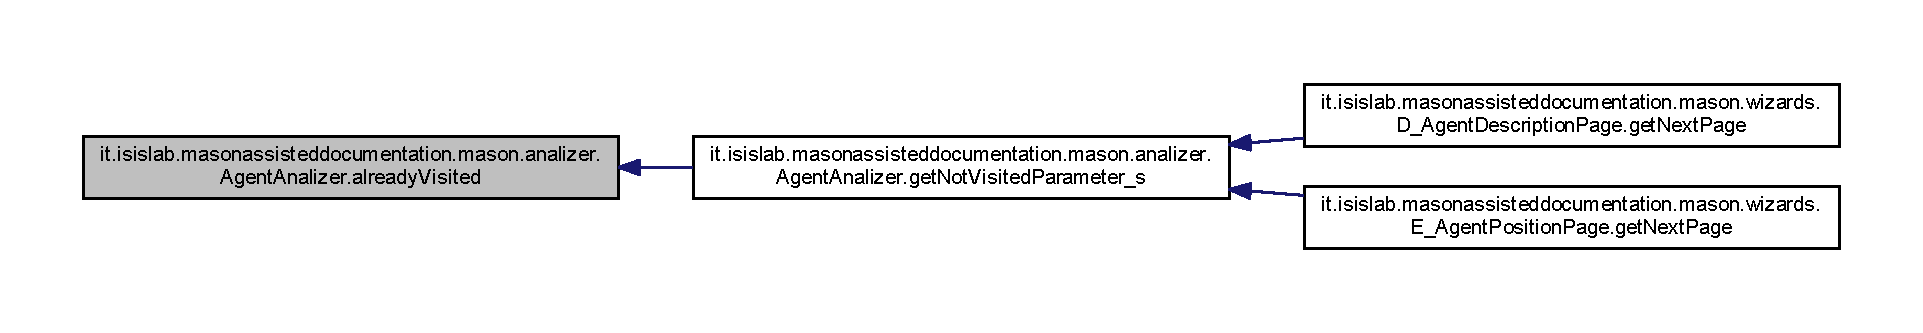
\includegraphics[width=350pt]{classit_1_1isislab_1_1masonassisteddocumentation_1_1mason_1_1analizer_1_1_agent_analizer_a3e5ea2154f20535f5bd33db685cf045c_icgraph}
\end{center}
\end{figure}


\hypertarget{classit_1_1isislab_1_1masonassisteddocumentation_1_1mason_1_1analizer_1_1_agent_analizer_a94492199c5e4873a07a2a46d15617937}{\index{it\-::isislab\-::masonassisteddocumentation\-::mason\-::analizer\-::\-Agent\-Analizer@{it\-::isislab\-::masonassisteddocumentation\-::mason\-::analizer\-::\-Agent\-Analizer}!get\-Class\-Name@{get\-Class\-Name}}
\index{get\-Class\-Name@{get\-Class\-Name}!it::isislab::masonassisteddocumentation::mason::analizer::AgentAnalizer@{it\-::isislab\-::masonassisteddocumentation\-::mason\-::analizer\-::\-Agent\-Analizer}}
\subsubsection[{get\-Class\-Name}]{\setlength{\rightskip}{0pt plus 5cm}String it.\-isislab.\-masonassisteddocumentation.\-mason.\-analizer.\-Agent\-Analizer.\-get\-Class\-Name (
\begin{DoxyParamCaption}
{}
\end{DoxyParamCaption}
)}}\label{classit_1_1isislab_1_1masonassisteddocumentation_1_1mason_1_1analizer_1_1_agent_analizer_a94492199c5e4873a07a2a46d15617937}
Return class name of this agent. \begin{DoxyReturn}{Returns}

\end{DoxyReturn}

\begin{DoxyCode}
175                                 \{
176         \textcolor{keywordflow}{return} agentICompilationUnit.getElementName();
177     \}
\end{DoxyCode}


Here is the caller graph for this function\-:\nopagebreak
\begin{figure}[H]
\begin{center}
\leavevmode
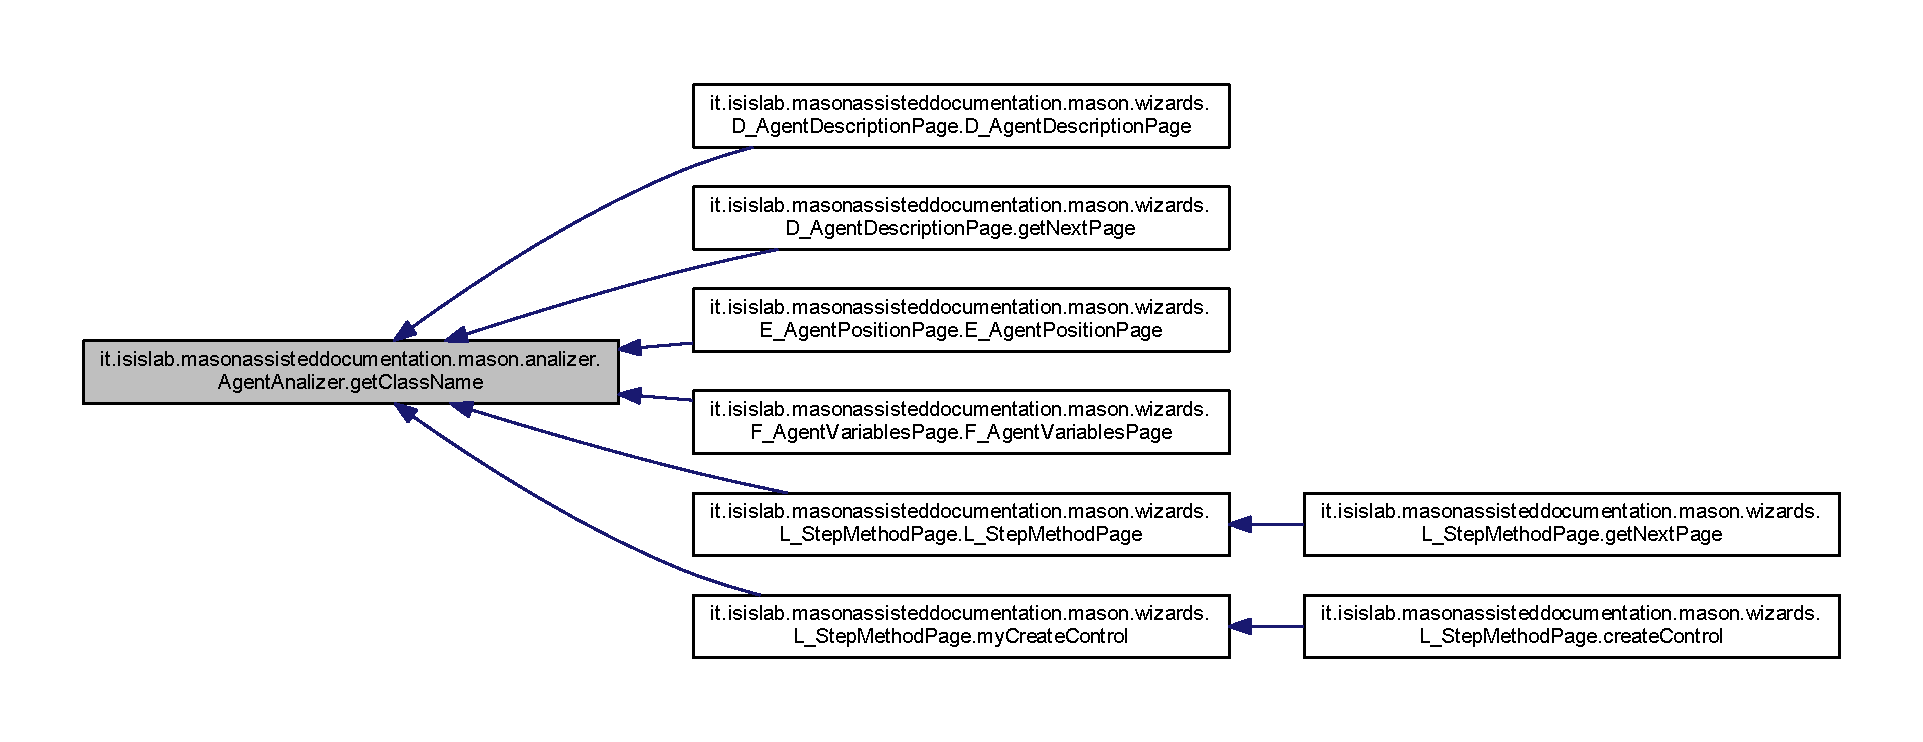
\includegraphics[width=350pt]{classit_1_1isislab_1_1masonassisteddocumentation_1_1mason_1_1analizer_1_1_agent_analizer_a94492199c5e4873a07a2a46d15617937_icgraph}
\end{center}
\end{figure}


\hypertarget{classit_1_1isislab_1_1masonassisteddocumentation_1_1mason_1_1analizer_1_1_agent_analizer_a452c584a7035bc8c4a550f4e86db8266}{\index{it\-::isislab\-::masonassisteddocumentation\-::mason\-::analizer\-::\-Agent\-Analizer@{it\-::isislab\-::masonassisteddocumentation\-::mason\-::analizer\-::\-Agent\-Analizer}!get\-Compilation\-Unit@{get\-Compilation\-Unit}}
\index{get\-Compilation\-Unit@{get\-Compilation\-Unit}!it::isislab::masonassisteddocumentation::mason::analizer::AgentAnalizer@{it\-::isislab\-::masonassisteddocumentation\-::mason\-::analizer\-::\-Agent\-Analizer}}
\subsubsection[{get\-Compilation\-Unit}]{\setlength{\rightskip}{0pt plus 5cm}Compilation\-Unit it.\-isislab.\-masonassisteddocumentation.\-mason.\-analizer.\-Agent\-Analizer.\-get\-Compilation\-Unit (
\begin{DoxyParamCaption}
{}
\end{DoxyParamCaption}
)}}\label{classit_1_1isislab_1_1masonassisteddocumentation_1_1mason_1_1analizer_1_1_agent_analizer_a452c584a7035bc8c4a550f4e86db8266}
Retirn Compilation\-Unit. \begin{DoxyReturn}{Returns}

\end{DoxyReturn}

\begin{DoxyCode}
125                                                \{
126         \textcolor{keywordflow}{return} \hyperlink{classit_1_1isislab_1_1masonassisteddocumentation_1_1mason_1_1analizer_1_1_agent_analizer_aad9b5d0882694d2802dc24c982f21985}{compilationUnit};
127     \}
\end{DoxyCode}


Here is the caller graph for this function\-:\nopagebreak
\begin{figure}[H]
\begin{center}
\leavevmode
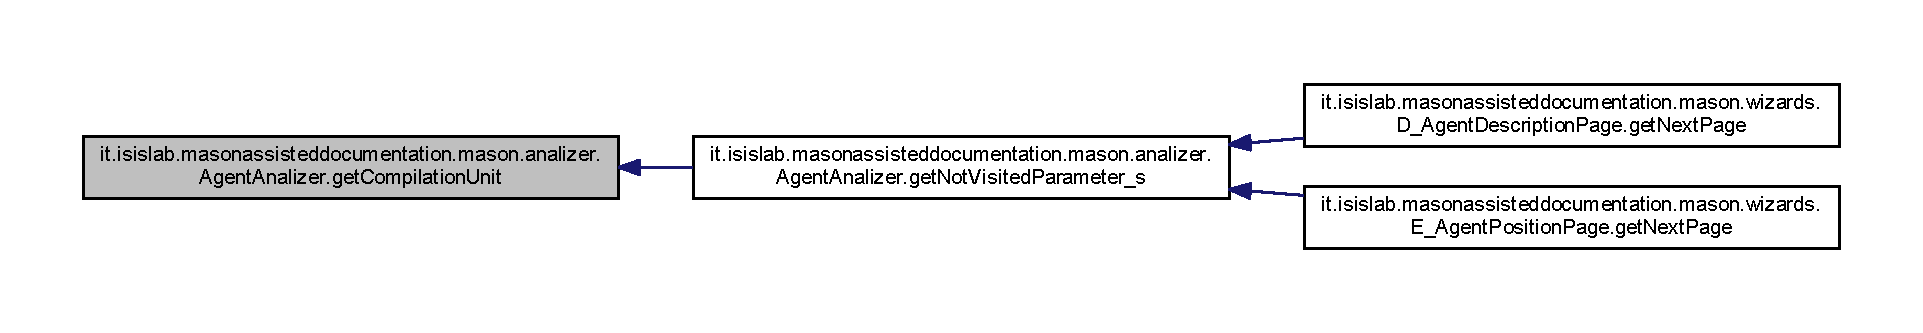
\includegraphics[width=350pt]{classit_1_1isislab_1_1masonassisteddocumentation_1_1mason_1_1analizer_1_1_agent_analizer_a452c584a7035bc8c4a550f4e86db8266_icgraph}
\end{center}
\end{figure}


\hypertarget{classit_1_1isislab_1_1masonassisteddocumentation_1_1mason_1_1analizer_1_1_agent_analizer_ae8de4d1c4186a27f567257c4b85c3f1c}{\index{it\-::isislab\-::masonassisteddocumentation\-::mason\-::analizer\-::\-Agent\-Analizer@{it\-::isislab\-::masonassisteddocumentation\-::mason\-::analizer\-::\-Agent\-Analizer}!get\-Model\-Description@{get\-Model\-Description}}
\index{get\-Model\-Description@{get\-Model\-Description}!it::isislab::masonassisteddocumentation::mason::analizer::AgentAnalizer@{it\-::isislab\-::masonassisteddocumentation\-::mason\-::analizer\-::\-Agent\-Analizer}}
\subsubsection[{get\-Model\-Description}]{\setlength{\rightskip}{0pt plus 5cm}Javadoc it.\-isislab.\-masonassisteddocumentation.\-mason.\-analizer.\-Agent\-Analizer.\-get\-Model\-Description (
\begin{DoxyParamCaption}
{}
\end{DoxyParamCaption}
)}}\label{classit_1_1isislab_1_1masonassisteddocumentation_1_1mason_1_1analizer_1_1_agent_analizer_ae8de4d1c4186a27f567257c4b85c3f1c}
This method return the descriprion of this Agent. \begin{DoxyReturn}{Returns}
Javadoc\-Comment if there is a description; else null. 
\end{DoxyReturn}

\begin{DoxyCode}
78                                         \{
79         List<TypeDeclaration> types = compilationUnit.types();
80         TypeDeclaration agent = types.get(0);
81         \textcolor{keywordflow}{return} agent.getJavadoc();
82     \}
\end{DoxyCode}
\hypertarget{classit_1_1isislab_1_1masonassisteddocumentation_1_1mason_1_1analizer_1_1_agent_analizer_ad237f6e49d6d49e0138b1e2ac6a2b0bb}{\index{it\-::isislab\-::masonassisteddocumentation\-::mason\-::analizer\-::\-Agent\-Analizer@{it\-::isislab\-::masonassisteddocumentation\-::mason\-::analizer\-::\-Agent\-Analizer}!get\-Not\-Visited\-Parameter\-\_\-s@{get\-Not\-Visited\-Parameter\-\_\-s}}
\index{get\-Not\-Visited\-Parameter\-\_\-s@{get\-Not\-Visited\-Parameter\-\_\-s}!it::isislab::masonassisteddocumentation::mason::analizer::AgentAnalizer@{it\-::isislab\-::masonassisteddocumentation\-::mason\-::analizer\-::\-Agent\-Analizer}}
\subsubsection[{get\-Not\-Visited\-Parameter\-\_\-s}]{\setlength{\rightskip}{0pt plus 5cm}Array\-List$<${\bf Parameter}$>$ it.\-isislab.\-masonassisteddocumentation.\-mason.\-analizer.\-Agent\-Analizer.\-get\-Not\-Visited\-Parameter\-\_\-s (
\begin{DoxyParamCaption}
{}
\end{DoxyParamCaption}
)}}\label{classit_1_1isislab_1_1masonassisteddocumentation_1_1mason_1_1analizer_1_1_agent_analizer_ad237f6e49d6d49e0138b1e2ac6a2b0bb}
Return parameter\-\_\-s that are not visited until now. \begin{DoxyReturn}{Returns}

\end{DoxyReturn}

\begin{DoxyCode}
163                                                           \{
164         ArrayList<Parameter> remainingParameters = \textcolor{keyword}{new} ArrayList<Parameter>();
165         ArrayList<Parameter> allParameters = GlobalUtility.getAllParameters(
      \hyperlink{classit_1_1isislab_1_1masonassisteddocumentation_1_1mason_1_1analizer_1_1_agent_analizer_a452c584a7035bc8c4a550f4e86db8266}{getCompilationUnit}());
166         \textcolor{keywordflow}{for} (Parameter p : allParameters)
167             \textcolor{keywordflow}{if} (!(\hyperlink{classit_1_1isislab_1_1masonassisteddocumentation_1_1mason_1_1analizer_1_1_agent_analizer_a3e5ea2154f20535f5bd33db685cf045c}{alreadyVisited}(p))) remainingParameters.add(p); 
168         \textcolor{keywordflow}{return} remainingParameters;
169     \}
\end{DoxyCode}


Here is the call graph for this function\-:\nopagebreak
\begin{figure}[H]
\begin{center}
\leavevmode
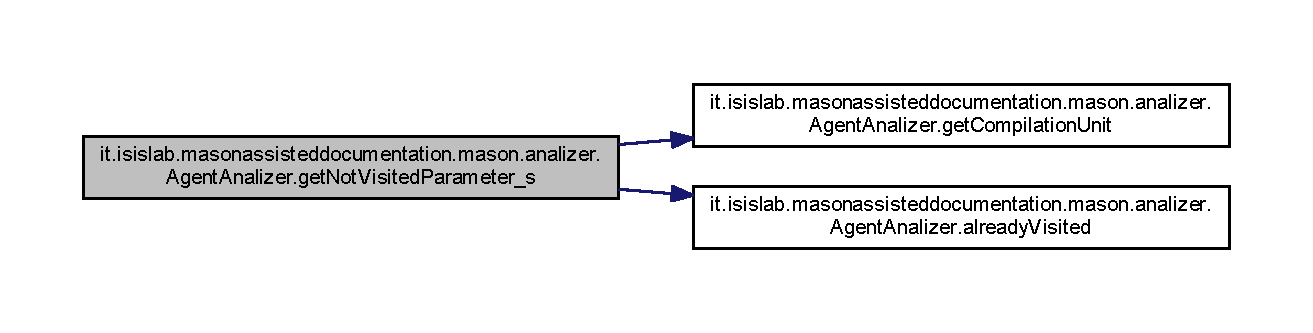
\includegraphics[width=350pt]{classit_1_1isislab_1_1masonassisteddocumentation_1_1mason_1_1analizer_1_1_agent_analizer_ad237f6e49d6d49e0138b1e2ac6a2b0bb_cgraph}
\end{center}
\end{figure}




Here is the caller graph for this function\-:\nopagebreak
\begin{figure}[H]
\begin{center}
\leavevmode
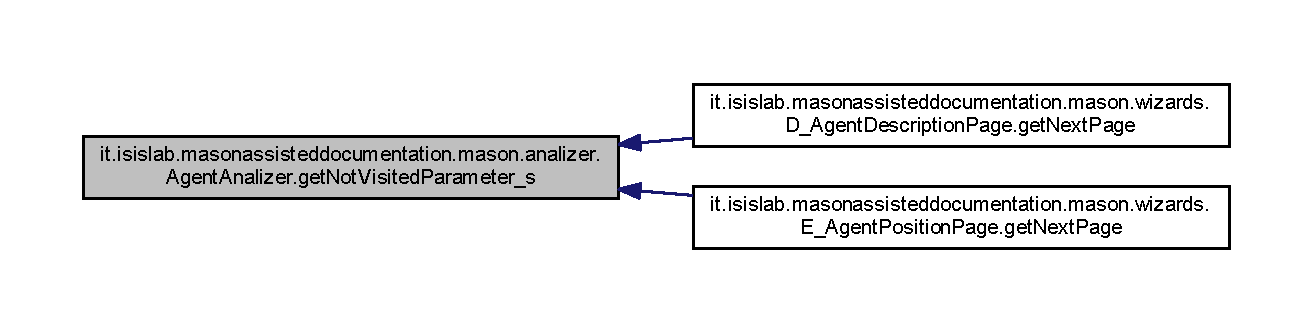
\includegraphics[width=350pt]{classit_1_1isislab_1_1masonassisteddocumentation_1_1mason_1_1analizer_1_1_agent_analizer_ad237f6e49d6d49e0138b1e2ac6a2b0bb_icgraph}
\end{center}
\end{figure}


\hypertarget{classit_1_1isislab_1_1masonassisteddocumentation_1_1mason_1_1analizer_1_1_agent_analizer_a3e46e6754b6575579be1a9ac062641fa}{\index{it\-::isislab\-::masonassisteddocumentation\-::mason\-::analizer\-::\-Agent\-Analizer@{it\-::isislab\-::masonassisteddocumentation\-::mason\-::analizer\-::\-Agent\-Analizer}!get\-Position\-Class@{get\-Position\-Class}}
\index{get\-Position\-Class@{get\-Position\-Class}!it::isislab::masonassisteddocumentation::mason::analizer::AgentAnalizer@{it\-::isislab\-::masonassisteddocumentation\-::mason\-::analizer\-::\-Agent\-Analizer}}
\subsubsection[{get\-Position\-Class}]{\setlength{\rightskip}{0pt plus 5cm}String it.\-isislab.\-masonassisteddocumentation.\-mason.\-analizer.\-Agent\-Analizer.\-get\-Position\-Class (
\begin{DoxyParamCaption}
{}
\end{DoxyParamCaption}
)}}\label{classit_1_1isislab_1_1masonassisteddocumentation_1_1mason_1_1analizer_1_1_agent_analizer_a3e46e6754b6575579be1a9ac062641fa}
Return a string representation of position\-Class array. \begin{DoxyReturn}{Returns}

\end{DoxyReturn}

\begin{DoxyCode}
137                                     \{
138         String toReturn = \textcolor{stringliteral}{""};
139         \textcolor{keywordflow}{for} (\textcolor{keywordtype}{int} i=0; i<positionClass.length; i++)\{
140             toReturn = toReturn + \hyperlink{classit_1_1isislab_1_1masonassisteddocumentation_1_1mason_1_1analizer_1_1_agent_analizer_aea5eff658e91428950dd0efd1339bf36}{positionClass}[i] + \textcolor{stringliteral}{" - "};
141         \}
142         \textcolor{keywordflow}{return} toReturn.substring(0, toReturn.length()-3);
143     \}
\end{DoxyCode}
\hypertarget{classit_1_1isislab_1_1masonassisteddocumentation_1_1mason_1_1analizer_1_1_agent_analizer_a351c38491d7f706177c4c76478cabd6d}{\index{it\-::isislab\-::masonassisteddocumentation\-::mason\-::analizer\-::\-Agent\-Analizer@{it\-::isislab\-::masonassisteddocumentation\-::mason\-::analizer\-::\-Agent\-Analizer}!get\-Positions\-Parameter@{get\-Positions\-Parameter}}
\index{get\-Positions\-Parameter@{get\-Positions\-Parameter}!it::isislab::masonassisteddocumentation::mason::analizer::AgentAnalizer@{it\-::isislab\-::masonassisteddocumentation\-::mason\-::analizer\-::\-Agent\-Analizer}}
\subsubsection[{get\-Positions\-Parameter}]{\setlength{\rightskip}{0pt plus 5cm}Array\-List$<${\bf Parameter}$>$ it.\-isislab.\-masonassisteddocumentation.\-mason.\-analizer.\-Agent\-Analizer.\-get\-Positions\-Parameter (
\begin{DoxyParamCaption}
{}
\end{DoxyParamCaption}
)}}\label{classit_1_1isislab_1_1masonassisteddocumentation_1_1mason_1_1analizer_1_1_agent_analizer_a351c38491d7f706177c4c76478cabd6d}
This method extract a list of Variable\-Declaration\-Fragment for positions variables. \begin{DoxyReturn}{Returns}
Array\-List of positions as Variable\-Declaration\-Fragment 
\end{DoxyReturn}

\begin{DoxyCode}
110                                                        \{
111         \textcolor{keywordflow}{if} (GlobalUtility.getAllParameters(\hyperlink{classit_1_1isislab_1_1masonassisteddocumentation_1_1mason_1_1analizer_1_1_agent_analizer_aad9b5d0882694d2802dc24c982f21985}{compilationUnit}) == null) \textcolor{keywordflow}{return} null;
112         ArrayList<Parameter> toReturn = \textcolor{keyword}{new} ArrayList<Parameter>();
113         \textcolor{keywordflow}{for} (Parameter p : GlobalUtility.getAllParameters(\hyperlink{classit_1_1isislab_1_1masonassisteddocumentation_1_1mason_1_1analizer_1_1_agent_analizer_aad9b5d0882694d2802dc24c982f21985}{compilationUnit}))\{
114                 \textcolor{keywordflow}{for} (\textcolor{keywordtype}{int} i=0; i<positionClass.length; i++)\{
115                     \textcolor{keywordflow}{if} (p.getVariableType().equalsIgnoreCase(\hyperlink{classit_1_1isislab_1_1masonassisteddocumentation_1_1mason_1_1analizer_1_1_agent_analizer_aea5eff658e91428950dd0efd1339bf36}{positionClass}[i]))    
      toReturn.add(p);
116                 \}               
117         \}
118         \textcolor{keywordflow}{return} toReturn;
119     \}   
\end{DoxyCode}


Here is the call graph for this function\-:\nopagebreak
\begin{figure}[H]
\begin{center}
\leavevmode
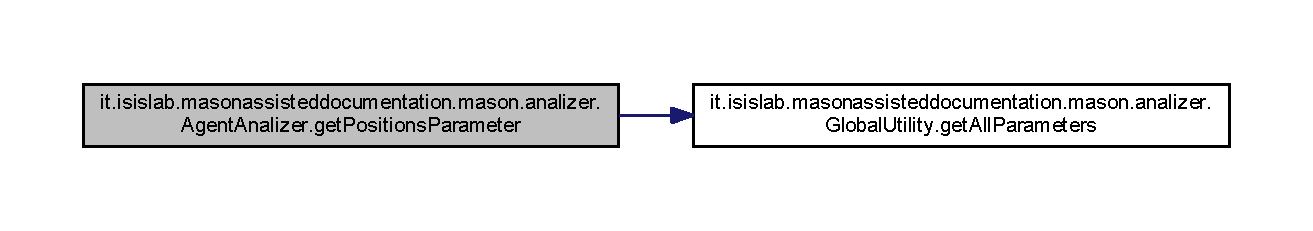
\includegraphics[width=350pt]{classit_1_1isislab_1_1masonassisteddocumentation_1_1mason_1_1analizer_1_1_agent_analizer_a351c38491d7f706177c4c76478cabd6d_cgraph}
\end{center}
\end{figure}




Here is the caller graph for this function\-:\nopagebreak
\begin{figure}[H]
\begin{center}
\leavevmode
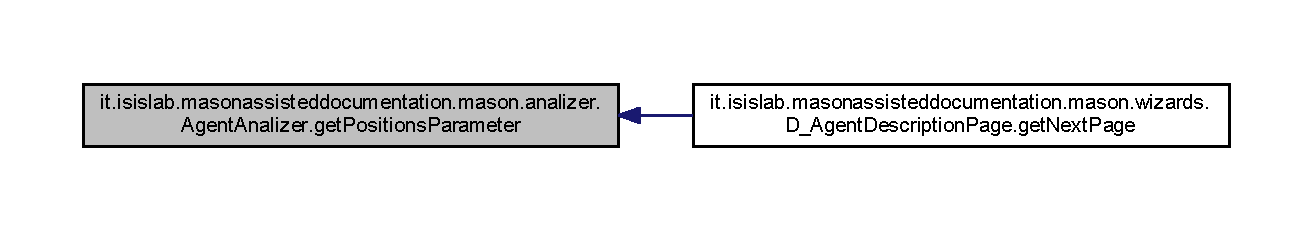
\includegraphics[width=350pt]{classit_1_1isislab_1_1masonassisteddocumentation_1_1mason_1_1analizer_1_1_agent_analizer_a351c38491d7f706177c4c76478cabd6d_icgraph}
\end{center}
\end{figure}


\hypertarget{classit_1_1isislab_1_1masonassisteddocumentation_1_1mason_1_1analizer_1_1_agent_analizer_a1ac3fc1c6fdf3133e81fba94fe13c01d}{\index{it\-::isislab\-::masonassisteddocumentation\-::mason\-::analizer\-::\-Agent\-Analizer@{it\-::isislab\-::masonassisteddocumentation\-::mason\-::analizer\-::\-Agent\-Analizer}!get\-Root@{get\-Root}}
\index{get\-Root@{get\-Root}!it::isislab::masonassisteddocumentation::mason::analizer::AgentAnalizer@{it\-::isislab\-::masonassisteddocumentation\-::mason\-::analizer\-::\-Agent\-Analizer}}
\subsubsection[{get\-Root}]{\setlength{\rightskip}{0pt plus 5cm}A\-S\-T it.\-isislab.\-masonassisteddocumentation.\-mason.\-analizer.\-Agent\-Analizer.\-get\-Root (
\begin{DoxyParamCaption}
{}
\end{DoxyParamCaption}
)}}\label{classit_1_1isislab_1_1masonassisteddocumentation_1_1mason_1_1analizer_1_1_agent_analizer_a1ac3fc1c6fdf3133e81fba94fe13c01d}

\begin{DoxyCode}
129                         \{
130         \textcolor{keywordflow}{return} \hyperlink{classit_1_1isislab_1_1masonassisteddocumentation_1_1mason_1_1analizer_1_1_agent_analizer_a83430d48ecbe1fc48d0cd8f10c2d99a8}{root};
131     \}
\end{DoxyCode}
\hypertarget{classit_1_1isislab_1_1masonassisteddocumentation_1_1mason_1_1analizer_1_1_agent_analizer_a76b619307dd702b85fc422f231fac76a}{\index{it\-::isislab\-::masonassisteddocumentation\-::mason\-::analizer\-::\-Agent\-Analizer@{it\-::isislab\-::masonassisteddocumentation\-::mason\-::analizer\-::\-Agent\-Analizer}!get\-Visited\-Parameters@{get\-Visited\-Parameters}}
\index{get\-Visited\-Parameters@{get\-Visited\-Parameters}!it::isislab::masonassisteddocumentation::mason::analizer::AgentAnalizer@{it\-::isislab\-::masonassisteddocumentation\-::mason\-::analizer\-::\-Agent\-Analizer}}
\subsubsection[{get\-Visited\-Parameters}]{\setlength{\rightskip}{0pt plus 5cm}Array\-List$<${\bf Parameter}$>$ it.\-isislab.\-masonassisteddocumentation.\-mason.\-analizer.\-Agent\-Analizer.\-get\-Visited\-Parameters (
\begin{DoxyParamCaption}
{}
\end{DoxyParamCaption}
)}}\label{classit_1_1isislab_1_1masonassisteddocumentation_1_1mason_1_1analizer_1_1_agent_analizer_a76b619307dd702b85fc422f231fac76a}
Return a list of visited parameter (visited means that parameters are already in Simulation\-Group). \begin{DoxyReturn}{Returns}

\end{DoxyReturn}

\begin{DoxyCode}
101                                                        \{
102         \textcolor{keywordflow}{return} \hyperlink{classit_1_1isislab_1_1masonassisteddocumentation_1_1mason_1_1analizer_1_1_agent_analizer_aee5454eb7063c444081bdb2556d3a60b}{visitedParameters};
103     \}
\end{DoxyCode}
\hypertarget{classit_1_1isislab_1_1masonassisteddocumentation_1_1mason_1_1analizer_1_1_agent_analizer_aa1cf97eff47c73e305fdd540a512a88c}{\index{it\-::isislab\-::masonassisteddocumentation\-::mason\-::analizer\-::\-Agent\-Analizer@{it\-::isislab\-::masonassisteddocumentation\-::mason\-::analizer\-::\-Agent\-Analizer}!rewrite@{rewrite}}
\index{rewrite@{rewrite}!it::isislab::masonassisteddocumentation::mason::analizer::AgentAnalizer@{it\-::isislab\-::masonassisteddocumentation\-::mason\-::analizer\-::\-Agent\-Analizer}}
\subsubsection[{rewrite}]{\setlength{\rightskip}{0pt plus 5cm}void it.\-isislab.\-masonassisteddocumentation.\-mason.\-analizer.\-Agent\-Analizer.\-rewrite (
\begin{DoxyParamCaption}
{}
\end{DoxyParamCaption}
)}}\label{classit_1_1isislab_1_1masonassisteddocumentation_1_1mason_1_1analizer_1_1_agent_analizer_aa1cf97eff47c73e305fdd540a512a88c}


Implements \hyperlink{interfaceit_1_1isislab_1_1masonassisteddocumentation_1_1mason_1_1analizer_1_1_analizer_a6b8cb1fad306066e18f05427fa306360}{it.\-isislab.\-masonassisteddocumentation.\-mason.\-analizer.\-Analizer}.


\begin{DoxyCode}
39                           \{
40         File sourceFile = \textcolor{keyword}{new} File(\hyperlink{classit_1_1isislab_1_1masonassisteddocumentation_1_1mason_1_1analizer_1_1_agent_analizer_ab0d7780b5d7b3607251116bf7bcde320}{agentICompilationUnit}.getResource().getRawLocation(
      ).toOSString());
41         FileOutputStream fooStream;
42         \textcolor{keywordflow}{try} \{
43             fooStream = \textcolor{keyword}{new} FileOutputStream(sourceFile, \textcolor{keyword}{false});
44             String code = compilationUnit.toString();
45             byte[] myBytes = code.getBytes();
46             fooStream.write(myBytes);
47             fooStream.close();
48         \} \textcolor{keywordflow}{catch} (FileNotFoundException e) \{
49             log.severe(\textcolor{stringliteral}{"Agent file not found to: "} + agentICompilationUnit.getResource().getRawLocation()
      .toOSString() + \textcolor{stringliteral}{"."});
50             e.printStackTrace();
51         \} \textcolor{keywordflow}{catch} (IOException e) \{
52             e.printStackTrace();
53         \}       
54     \}
\end{DoxyCode}
\hypertarget{classit_1_1isislab_1_1masonassisteddocumentation_1_1mason_1_1analizer_1_1_agent_analizer_afd9a63275f03a03ca69187b8cce6613e}{\index{it\-::isislab\-::masonassisteddocumentation\-::mason\-::analizer\-::\-Agent\-Analizer@{it\-::isislab\-::masonassisteddocumentation\-::mason\-::analizer\-::\-Agent\-Analizer}!rewrite@{rewrite}}
\index{rewrite@{rewrite}!it::isislab::masonassisteddocumentation::mason::analizer::AgentAnalizer@{it\-::isislab\-::masonassisteddocumentation\-::mason\-::analizer\-::\-Agent\-Analizer}}
\subsubsection[{rewrite}]{\setlength{\rightskip}{0pt plus 5cm}void it.\-isislab.\-masonassisteddocumentation.\-mason.\-analizer.\-Agent\-Analizer.\-rewrite (
\begin{DoxyParamCaption}
\item[{String}]{path\-Name}
\end{DoxyParamCaption}
)}}\label{classit_1_1isislab_1_1masonassisteddocumentation_1_1mason_1_1analizer_1_1_agent_analizer_afd9a63275f03a03ca69187b8cce6613e}

\begin{DoxyCode}
56                                         \{
57         File sourceFile = \textcolor{keyword}{new} File(pathName);
58         FileOutputStream fooStream;
59         \textcolor{keywordflow}{try} \{
60             fooStream = \textcolor{keyword}{new} FileOutputStream(sourceFile, \textcolor{keyword}{false});
61             String code = compilationUnit.toString();
62             byte[] myBytes = code.getBytes();
63             fooStream.write(myBytes);
64             fooStream.close();
65         \} \textcolor{keywordflow}{catch} (FileNotFoundException e) \{
66             log.severe(\textcolor{stringliteral}{"Agent file not found to: "} + pathName + \textcolor{stringliteral}{"."});
67             e.printStackTrace();
68         \} \textcolor{keywordflow}{catch} (IOException e) \{
69             e.printStackTrace();
70         \}   
71     \}
\end{DoxyCode}
\hypertarget{classit_1_1isislab_1_1masonassisteddocumentation_1_1mason_1_1analizer_1_1_agent_analizer_aaef67e385b42699bd863f505be5df17d}{\index{it\-::isislab\-::masonassisteddocumentation\-::mason\-::analizer\-::\-Agent\-Analizer@{it\-::isislab\-::masonassisteddocumentation\-::mason\-::analizer\-::\-Agent\-Analizer}!set\-Class\-Description@{set\-Class\-Description}}
\index{set\-Class\-Description@{set\-Class\-Description}!it::isislab::masonassisteddocumentation::mason::analizer::AgentAnalizer@{it\-::isislab\-::masonassisteddocumentation\-::mason\-::analizer\-::\-Agent\-Analizer}}
\subsubsection[{set\-Class\-Description}]{\setlength{\rightskip}{0pt plus 5cm}void it.\-isislab.\-masonassisteddocumentation.\-mason.\-analizer.\-Agent\-Analizer.\-set\-Class\-Description (
\begin{DoxyParamCaption}
\item[{String}]{model\-Description}
\end{DoxyParamCaption}
)}}\label{classit_1_1isislab_1_1masonassisteddocumentation_1_1mason_1_1analizer_1_1_agent_analizer_aaef67e385b42699bd863f505be5df17d}
This method set the description of model to model\-Description value. 
\begin{DoxyParams}{Parameters}
{\em model\-Description} & \\
\hline
\end{DoxyParams}

\begin{DoxyCode}
89                                                             \{
90         List<TypeDeclaration> types = compilationUnit.types();      
91         TypeDeclaration agent = types.get(0);   \textcolor{comment}{//get class definition (element in position 0)}
92         modelDescription = GlobalUtility.COMMENT\_SIGNATURE + \textcolor{stringliteral}{"@ingroup entities\(\backslash\)n*\(\backslash\)n*"} + 
      GlobalUtility.surroundWithSpan(\hyperlink{classit_1_1isislab_1_1masonassisteddocumentation_1_1mason_1_1analizer_1_1_global_utility_a0fcb324ae33eb93bd5b9177e342ecc82}{GlobalUtility.userOutputColor}, modelDescription);  
93         GlobalUtility.setJavadocToType(\hyperlink{classit_1_1isislab_1_1masonassisteddocumentation_1_1mason_1_1analizer_1_1_agent_analizer_a83430d48ecbe1fc48d0cd8f10c2d99a8}{root}, agent, modelDescription);
94     \}
\end{DoxyCode}
\hypertarget{classit_1_1isislab_1_1masonassisteddocumentation_1_1mason_1_1analizer_1_1_agent_analizer_aa1e783609d0c0ffbb244ba4c22abc7b9}{\index{it\-::isislab\-::masonassisteddocumentation\-::mason\-::analizer\-::\-Agent\-Analizer@{it\-::isislab\-::masonassisteddocumentation\-::mason\-::analizer\-::\-Agent\-Analizer}!to\-String@{to\-String}}
\index{to\-String@{to\-String}!it::isislab::masonassisteddocumentation::mason::analizer::AgentAnalizer@{it\-::isislab\-::masonassisteddocumentation\-::mason\-::analizer\-::\-Agent\-Analizer}}
\subsubsection[{to\-String}]{\setlength{\rightskip}{0pt plus 5cm}String it.\-isislab.\-masonassisteddocumentation.\-mason.\-analizer.\-Agent\-Analizer.\-to\-String (
\begin{DoxyParamCaption}
{}
\end{DoxyParamCaption}
)}}\label{classit_1_1isislab_1_1masonassisteddocumentation_1_1mason_1_1analizer_1_1_agent_analizer_aa1e783609d0c0ffbb244ba4c22abc7b9}

\begin{DoxyCode}
179                             \{
180         \textcolor{keywordflow}{return} compilationUnit.toString();
181     \}
\end{DoxyCode}


\subsection{Member Data Documentation}
\hypertarget{classit_1_1isislab_1_1masonassisteddocumentation_1_1mason_1_1analizer_1_1_agent_analizer_ab0d7780b5d7b3607251116bf7bcde320}{\index{it\-::isislab\-::masonassisteddocumentation\-::mason\-::analizer\-::\-Agent\-Analizer@{it\-::isislab\-::masonassisteddocumentation\-::mason\-::analizer\-::\-Agent\-Analizer}!agent\-I\-Compilation\-Unit@{agent\-I\-Compilation\-Unit}}
\index{agent\-I\-Compilation\-Unit@{agent\-I\-Compilation\-Unit}!it::isislab::masonassisteddocumentation::mason::analizer::AgentAnalizer@{it\-::isislab\-::masonassisteddocumentation\-::mason\-::analizer\-::\-Agent\-Analizer}}
\subsubsection[{agent\-I\-Compilation\-Unit}]{\setlength{\rightskip}{0pt plus 5cm}I\-Compilation\-Unit it.\-isislab.\-masonassisteddocumentation.\-mason.\-analizer.\-Agent\-Analizer.\-agent\-I\-Compilation\-Unit\hspace{0.3cm}{\ttfamily [private]}}}\label{classit_1_1isislab_1_1masonassisteddocumentation_1_1mason_1_1analizer_1_1_agent_analizer_ab0d7780b5d7b3607251116bf7bcde320}
\hypertarget{classit_1_1isislab_1_1masonassisteddocumentation_1_1mason_1_1analizer_1_1_agent_analizer_aad9b5d0882694d2802dc24c982f21985}{\index{it\-::isislab\-::masonassisteddocumentation\-::mason\-::analizer\-::\-Agent\-Analizer@{it\-::isislab\-::masonassisteddocumentation\-::mason\-::analizer\-::\-Agent\-Analizer}!compilation\-Unit@{compilation\-Unit}}
\index{compilation\-Unit@{compilation\-Unit}!it::isislab::masonassisteddocumentation::mason::analizer::AgentAnalizer@{it\-::isislab\-::masonassisteddocumentation\-::mason\-::analizer\-::\-Agent\-Analizer}}
\subsubsection[{compilation\-Unit}]{\setlength{\rightskip}{0pt plus 5cm}Compilation\-Unit it.\-isislab.\-masonassisteddocumentation.\-mason.\-analizer.\-Agent\-Analizer.\-compilation\-Unit\hspace{0.3cm}{\ttfamily [private]}}}\label{classit_1_1isislab_1_1masonassisteddocumentation_1_1mason_1_1analizer_1_1_agent_analizer_aad9b5d0882694d2802dc24c982f21985}
\hypertarget{classit_1_1isislab_1_1masonassisteddocumentation_1_1mason_1_1analizer_1_1_agent_analizer_ad9766d313bd07461a473e31b771c26c6}{\index{it\-::isislab\-::masonassisteddocumentation\-::mason\-::analizer\-::\-Agent\-Analizer@{it\-::isislab\-::masonassisteddocumentation\-::mason\-::analizer\-::\-Agent\-Analizer}!log@{log}}
\index{log@{log}!it::isislab::masonassisteddocumentation::mason::analizer::AgentAnalizer@{it\-::isislab\-::masonassisteddocumentation\-::mason\-::analizer\-::\-Agent\-Analizer}}
\subsubsection[{log}]{\setlength{\rightskip}{0pt plus 5cm}Logger it.\-isislab.\-masonassisteddocumentation.\-mason.\-analizer.\-Agent\-Analizer.\-log = Logger.\-get\-Logger(\char`\"{}global\char`\"{})\hspace{0.3cm}{\ttfamily [static]}, {\ttfamily [private]}}}\label{classit_1_1isislab_1_1masonassisteddocumentation_1_1mason_1_1analizer_1_1_agent_analizer_ad9766d313bd07461a473e31b771c26c6}
\hypertarget{classit_1_1isislab_1_1masonassisteddocumentation_1_1mason_1_1analizer_1_1_agent_analizer_aea5eff658e91428950dd0efd1339bf36}{\index{it\-::isislab\-::masonassisteddocumentation\-::mason\-::analizer\-::\-Agent\-Analizer@{it\-::isislab\-::masonassisteddocumentation\-::mason\-::analizer\-::\-Agent\-Analizer}!position\-Class@{position\-Class}}
\index{position\-Class@{position\-Class}!it::isislab::masonassisteddocumentation::mason::analizer::AgentAnalizer@{it\-::isislab\-::masonassisteddocumentation\-::mason\-::analizer\-::\-Agent\-Analizer}}
\subsubsection[{position\-Class}]{\setlength{\rightskip}{0pt plus 5cm}String \mbox{[}$\,$\mbox{]} it.\-isislab.\-masonassisteddocumentation.\-mason.\-analizer.\-Agent\-Analizer.\-position\-Class = \{\char`\"{}Int2\-D\char`\"{}, \char`\"{}Double2\-D\char`\"{}, \char`\"{}Int3\-D\char`\"{}, \char`\"{}Double3\-D\char`\"{},\}\hspace{0.3cm}{\ttfamily [static]}}}\label{classit_1_1isislab_1_1masonassisteddocumentation_1_1mason_1_1analizer_1_1_agent_analizer_aea5eff658e91428950dd0efd1339bf36}
\hypertarget{classit_1_1isislab_1_1masonassisteddocumentation_1_1mason_1_1analizer_1_1_agent_analizer_a83430d48ecbe1fc48d0cd8f10c2d99a8}{\index{it\-::isislab\-::masonassisteddocumentation\-::mason\-::analizer\-::\-Agent\-Analizer@{it\-::isislab\-::masonassisteddocumentation\-::mason\-::analizer\-::\-Agent\-Analizer}!root@{root}}
\index{root@{root}!it::isislab::masonassisteddocumentation::mason::analizer::AgentAnalizer@{it\-::isislab\-::masonassisteddocumentation\-::mason\-::analizer\-::\-Agent\-Analizer}}
\subsubsection[{root}]{\setlength{\rightskip}{0pt plus 5cm}A\-S\-T it.\-isislab.\-masonassisteddocumentation.\-mason.\-analizer.\-Agent\-Analizer.\-root\hspace{0.3cm}{\ttfamily [private]}}}\label{classit_1_1isislab_1_1masonassisteddocumentation_1_1mason_1_1analizer_1_1_agent_analizer_a83430d48ecbe1fc48d0cd8f10c2d99a8}
\hypertarget{classit_1_1isislab_1_1masonassisteddocumentation_1_1mason_1_1analizer_1_1_agent_analizer_a5c6d63f226ee1dc2a0749c6a5ee40dd9}{\index{it\-::isislab\-::masonassisteddocumentation\-::mason\-::analizer\-::\-Agent\-Analizer@{it\-::isislab\-::masonassisteddocumentation\-::mason\-::analizer\-::\-Agent\-Analizer}!steppable\-Description@{steppable\-Description}}
\index{steppable\-Description@{steppable\-Description}!it::isislab::masonassisteddocumentation::mason::analizer::AgentAnalizer@{it\-::isislab\-::masonassisteddocumentation\-::mason\-::analizer\-::\-Agent\-Analizer}}
\subsubsection[{steppable\-Description}]{\setlength{\rightskip}{0pt plus 5cm}String it.\-isislab.\-masonassisteddocumentation.\-mason.\-analizer.\-Agent\-Analizer.\-steppable\-Description\hspace{0.3cm}{\ttfamily [static]}}}\label{classit_1_1isislab_1_1masonassisteddocumentation_1_1mason_1_1analizer_1_1_agent_analizer_a5c6d63f226ee1dc2a0749c6a5ee40dd9}
{\bfseries Initial value\-:}
\begin{DoxyCode}
= \textcolor{stringliteral}{"By being Steppable, this class represent an agent that can be\(\backslash\)n"}
            + \textcolor{stringliteral}{"on the Schedule to have its step method called at various times\(\backslash\)n"}
            + \textcolor{stringliteral}{"int the future. This graduates this agent from being a mere object\(\backslash\)n"}
            + \textcolor{stringliteral}{" in the simulation to being something potentially approximating a real agent.\(\backslash\)n"}
            + \textcolor{stringliteral}{"When this agent is stepped, it is passed the SimState.\(\backslash\)n"}
\end{DoxyCode}
\hypertarget{classit_1_1isislab_1_1masonassisteddocumentation_1_1mason_1_1analizer_1_1_agent_analizer_aee5454eb7063c444081bdb2556d3a60b}{\index{it\-::isislab\-::masonassisteddocumentation\-::mason\-::analizer\-::\-Agent\-Analizer@{it\-::isislab\-::masonassisteddocumentation\-::mason\-::analizer\-::\-Agent\-Analizer}!visited\-Parameters@{visited\-Parameters}}
\index{visited\-Parameters@{visited\-Parameters}!it::isislab::masonassisteddocumentation::mason::analizer::AgentAnalizer@{it\-::isislab\-::masonassisteddocumentation\-::mason\-::analizer\-::\-Agent\-Analizer}}
\subsubsection[{visited\-Parameters}]{\setlength{\rightskip}{0pt plus 5cm}Array\-List$<${\bf Parameter}$>$ it.\-isislab.\-masonassisteddocumentation.\-mason.\-analizer.\-Agent\-Analizer.\-visited\-Parameters\hspace{0.3cm}{\ttfamily [private]}}}\label{classit_1_1isislab_1_1masonassisteddocumentation_1_1mason_1_1analizer_1_1_agent_analizer_aee5454eb7063c444081bdb2556d3a60b}


The documentation for this class was generated from the following file\-:\begin{DoxyCompactItemize}
\item 
src/it/isislab/masonassisteddocumentation/mason/analizer/\hyperlink{_agent_analizer_8java}{Agent\-Analizer.\-java}\end{DoxyCompactItemize}

\hypertarget{interfaceit_1_1isislab_1_1masonassisteddocumentation_1_1mason_1_1analizer_1_1_analizer}{\section{it.\-isislab.\-masonassisteddocumentation.\-mason.\-analizer.\-Analizer Interface Reference}
\label{interfaceit_1_1isislab_1_1masonassisteddocumentation_1_1mason_1_1analizer_1_1_analizer}\index{it.\-isislab.\-masonassisteddocumentation.\-mason.\-analizer.\-Analizer@{it.\-isislab.\-masonassisteddocumentation.\-mason.\-analizer.\-Analizer}}
}


Inheritance diagram for it.\-isislab.\-masonassisteddocumentation.\-mason.\-analizer.\-Analizer\-:
\nopagebreak
\begin{figure}[H]
\begin{center}
\leavevmode
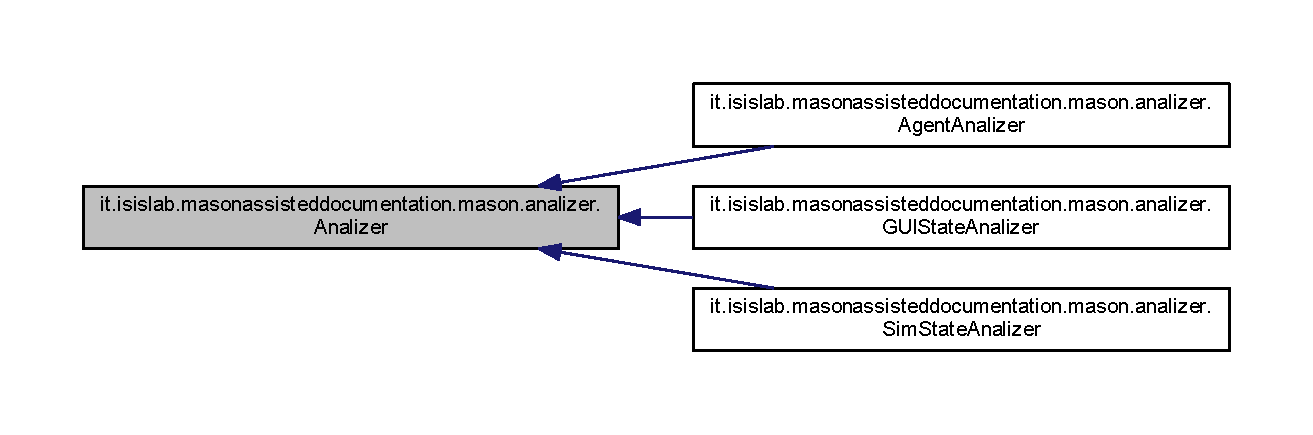
\includegraphics[width=350pt]{interfaceit_1_1isislab_1_1masonassisteddocumentation_1_1mason_1_1analizer_1_1_analizer__inherit__graph}
\end{center}
\end{figure}
\subsection*{Public Member Functions}
\begin{DoxyCompactItemize}
\item 
void \hyperlink{interfaceit_1_1isislab_1_1masonassisteddocumentation_1_1mason_1_1analizer_1_1_analizer_a6b8cb1fad306066e18f05427fa306360}{rewrite} ()
\end{DoxyCompactItemize}


\subsection{Member Function Documentation}
\hypertarget{interfaceit_1_1isislab_1_1masonassisteddocumentation_1_1mason_1_1analizer_1_1_analizer_a6b8cb1fad306066e18f05427fa306360}{\index{it\-::isislab\-::masonassisteddocumentation\-::mason\-::analizer\-::\-Analizer@{it\-::isislab\-::masonassisteddocumentation\-::mason\-::analizer\-::\-Analizer}!rewrite@{rewrite}}
\index{rewrite@{rewrite}!it::isislab::masonassisteddocumentation::mason::analizer::Analizer@{it\-::isislab\-::masonassisteddocumentation\-::mason\-::analizer\-::\-Analizer}}
\subsubsection[{rewrite}]{\setlength{\rightskip}{0pt plus 5cm}void it.\-isislab.\-masonassisteddocumentation.\-mason.\-analizer.\-Analizer.\-rewrite (
\begin{DoxyParamCaption}
{}
\end{DoxyParamCaption}
)}}\label{interfaceit_1_1isislab_1_1masonassisteddocumentation_1_1mason_1_1analizer_1_1_analizer_a6b8cb1fad306066e18f05427fa306360}


Implemented in \hyperlink{classit_1_1isislab_1_1masonassisteddocumentation_1_1mason_1_1analizer_1_1_sim_state_analizer_a9638ebfd96b5ecd957ff1798f15e4621}{it.\-isislab.\-masonassisteddocumentation.\-mason.\-analizer.\-Sim\-State\-Analizer}, \hyperlink{classit_1_1isislab_1_1masonassisteddocumentation_1_1mason_1_1analizer_1_1_g_u_i_state_analizer_a247ba9e4d8bcb9fe8266f0de15cae65f}{it.\-isislab.\-masonassisteddocumentation.\-mason.\-analizer.\-G\-U\-I\-State\-Analizer}, and \hyperlink{classit_1_1isislab_1_1masonassisteddocumentation_1_1mason_1_1analizer_1_1_agent_analizer_aa1cf97eff47c73e305fdd540a512a88c}{it.\-isislab.\-masonassisteddocumentation.\-mason.\-analizer.\-Agent\-Analizer}.



The documentation for this interface was generated from the following file\-:\begin{DoxyCompactItemize}
\item 
src/it/isislab/masonassisteddocumentation/mason/analizer/\hyperlink{_analizer_8java}{Analizer.\-java}\end{DoxyCompactItemize}

\hypertarget{classit_1_1isislab_1_1masonassisteddocumentation_1_1mason_1_1wizards_1_1_b___project_information_page}{\section{it.\-isislab.\-masonassisteddocumentation.\-mason.\-wizards.\-B\-\_\-\-Project\-Information\-Page Class Reference}
\label{classit_1_1isislab_1_1masonassisteddocumentation_1_1mason_1_1wizards_1_1_b___project_information_page}\index{it.\-isislab.\-masonassisteddocumentation.\-mason.\-wizards.\-B\-\_\-\-Project\-Information\-Page@{it.\-isislab.\-masonassisteddocumentation.\-mason.\-wizards.\-B\-\_\-\-Project\-Information\-Page}}
}


Inheritance diagram for it.\-isislab.\-masonassisteddocumentation.\-mason.\-wizards.\-B\-\_\-\-Project\-Information\-Page\-:\nopagebreak
\begin{figure}[H]
\begin{center}
\leavevmode
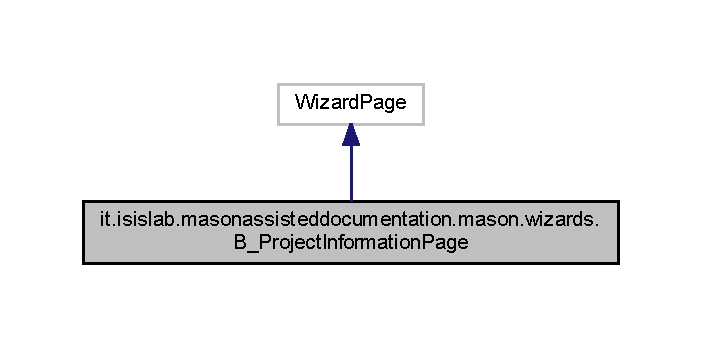
\includegraphics[width=337pt]{classit_1_1isislab_1_1masonassisteddocumentation_1_1mason_1_1wizards_1_1_b___project_information_page__inherit__graph}
\end{center}
\end{figure}


Collaboration diagram for it.\-isislab.\-masonassisteddocumentation.\-mason.\-wizards.\-B\-\_\-\-Project\-Information\-Page\-:\nopagebreak
\begin{figure}[H]
\begin{center}
\leavevmode
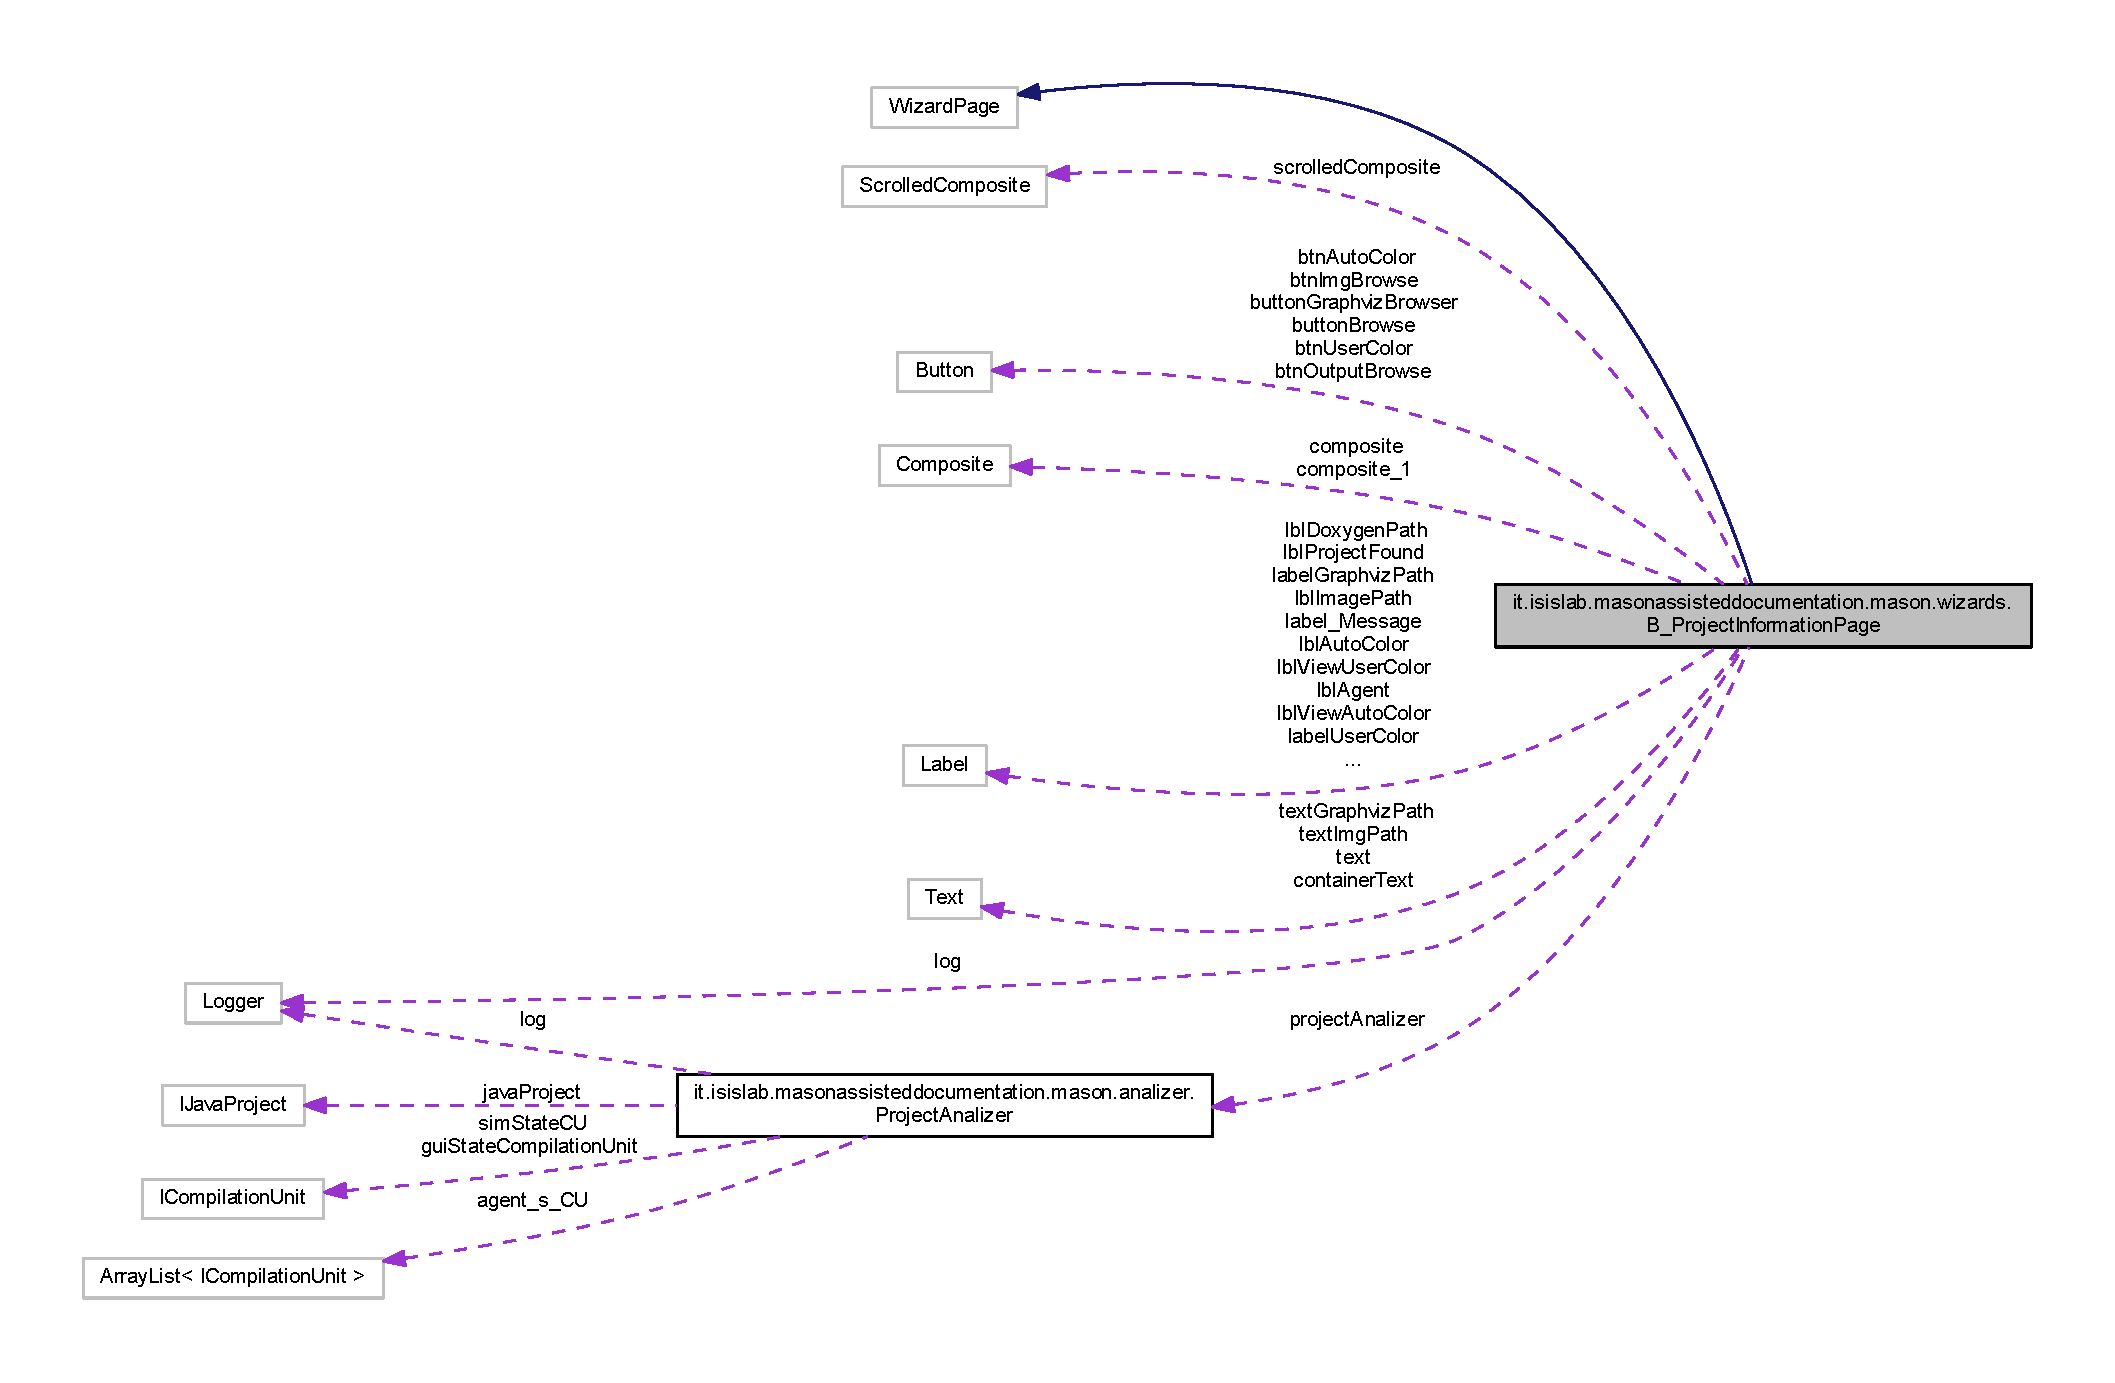
\includegraphics[width=350pt]{classit_1_1isislab_1_1masonassisteddocumentation_1_1mason_1_1wizards_1_1_b___project_information_page__coll__graph}
\end{center}
\end{figure}
\subsection*{Public Member Functions}
\begin{DoxyCompactItemize}
\item 
\hyperlink{classit_1_1isislab_1_1masonassisteddocumentation_1_1mason_1_1wizards_1_1_b___project_information_page_a2e67ccd1816ffe847ad99b57bc6bfdad}{B\-\_\-\-Project\-Information\-Page} ()
\item 
boolean \hyperlink{classit_1_1isislab_1_1masonassisteddocumentation_1_1mason_1_1wizards_1_1_b___project_information_page_a5b4f818a204c8f8a1934ceaf016cabd7}{is\-Doxygen\-Path\-Set} ()
\item 
void \hyperlink{classit_1_1isislab_1_1masonassisteddocumentation_1_1mason_1_1wizards_1_1_b___project_information_page_ab664591c88285aa5d3cc990620e812dd}{create\-Control} (Composite parent)
\item 
boolean \hyperlink{classit_1_1isislab_1_1masonassisteddocumentation_1_1mason_1_1wizards_1_1_b___project_information_page_a4ad2c0b1269d22b81ffc9e77f399c6af}{can\-Flip\-To\-Next\-Page} ()
\item 
boolean \hyperlink{classit_1_1isislab_1_1masonassisteddocumentation_1_1mason_1_1wizards_1_1_b___project_information_page_a86f79621a6b3201e70a35c54ec1e8c3f}{is\-Page\-Complete} ()
\item 
I\-Wizard\-Page \hyperlink{classit_1_1isislab_1_1masonassisteddocumentation_1_1mason_1_1wizards_1_1_b___project_information_page_a62abef1230b2c72e555e530004e4c5f9}{get\-Next\-Page} ()
\end{DoxyCompactItemize}
\subsection*{Private Member Functions}
\begin{DoxyCompactItemize}
\item 
void \hyperlink{classit_1_1isislab_1_1masonassisteddocumentation_1_1mason_1_1wizards_1_1_b___project_information_page_ad0acda6e90aee0af403c3e9c53525b5d}{set\-Doxygen\-Label\-Path\-From\-Config} ()
\item 
void \hyperlink{classit_1_1isislab_1_1masonassisteddocumentation_1_1mason_1_1wizards_1_1_b___project_information_page_af5afa21c1d0087572ad8b3d0a1a1fe9c}{set\-Project\-Label} ()
\end{DoxyCompactItemize}
\subsection*{Private Attributes}
\begin{DoxyCompactItemize}
\item 
Text \hyperlink{classit_1_1isislab_1_1masonassisteddocumentation_1_1mason_1_1wizards_1_1_b___project_information_page_afd09135c84c569cc68148a0166b9390a}{container\-Text}
\item 
Label \hyperlink{classit_1_1isislab_1_1masonassisteddocumentation_1_1mason_1_1wizards_1_1_b___project_information_page_a4887707c3be26291594a2d0010abd500}{lbl\-Doxygen\-Path}
\item 
Button \hyperlink{classit_1_1isislab_1_1masonassisteddocumentation_1_1mason_1_1wizards_1_1_b___project_information_page_a0962e195aa316ea8c931a45b59971432}{button\-Browse}
\item 
\hyperlink{classit_1_1isislab_1_1masonassisteddocumentation_1_1mason_1_1analizer_1_1_project_analizer}{Project\-Analizer} \hyperlink{classit_1_1isislab_1_1masonassisteddocumentation_1_1mason_1_1wizards_1_1_b___project_information_page_a5129feb0fa34a1d51e44a2fe495ac42c}{project\-Analizer}
\item 
Label \hyperlink{classit_1_1isislab_1_1masonassisteddocumentation_1_1mason_1_1wizards_1_1_b___project_information_page_a6c9ce7d939e8bd032a1f2fb5e42f0d78}{lbl\-Image\-Path}
\item 
Text \hyperlink{classit_1_1isislab_1_1masonassisteddocumentation_1_1mason_1_1wizards_1_1_b___project_information_page_a1217897a98e0714c9e7d8141b4e931d1}{text\-Img\-Path}
\item 
Button \hyperlink{classit_1_1isislab_1_1masonassisteddocumentation_1_1mason_1_1wizards_1_1_b___project_information_page_a6afdf6ba02f0bf721af2acd61a2a1a5c}{btn\-Img\-Browse}
\item 
Text \hyperlink{classit_1_1isislab_1_1masonassisteddocumentation_1_1mason_1_1wizards_1_1_b___project_information_page_aae0eab045b1d0530a794116410ae6e5d}{text}
\item 
Button \hyperlink{classit_1_1isislab_1_1masonassisteddocumentation_1_1mason_1_1wizards_1_1_b___project_information_page_a0cbfd9890c8c62af7cfce149089682b5}{btn\-Output\-Browse}
\item 
Label \hyperlink{classit_1_1isislab_1_1masonassisteddocumentation_1_1mason_1_1wizards_1_1_b___project_information_page_acb48412dbb797258e13404c757c8d3f4}{label\-Graphviz\-Path}
\item 
Text \hyperlink{classit_1_1isislab_1_1masonassisteddocumentation_1_1mason_1_1wizards_1_1_b___project_information_page_a03d43e1fbcdb5d7d5e6745d8f57db84b}{text\-Graphviz\-Path}
\item 
Button \hyperlink{classit_1_1isislab_1_1masonassisteddocumentation_1_1mason_1_1wizards_1_1_b___project_information_page_ad5db74dd5c7fc084f538fde88d57573a}{button\-Graphviz\-Browser}
\item 
Scrolled\-Composite \hyperlink{classit_1_1isislab_1_1masonassisteddocumentation_1_1mason_1_1wizards_1_1_b___project_information_page_adf33db8f408e4f486a256d199eae3bae}{scrolled\-Composite}
\item 
Composite \hyperlink{classit_1_1isislab_1_1masonassisteddocumentation_1_1mason_1_1wizards_1_1_b___project_information_page_abff2b9b46293282381b6cd1b26f83792}{composite}
\item 
Label \hyperlink{classit_1_1isislab_1_1masonassisteddocumentation_1_1mason_1_1wizards_1_1_b___project_information_page_a801e6444bc2096376ffbfd62f2660aaf}{lbl\-Project\-Found}
\item 
Label \hyperlink{classit_1_1isislab_1_1masonassisteddocumentation_1_1mason_1_1wizards_1_1_b___project_information_page_a65bb7c12ddee14a56433fb0af2e97e89}{lbl\-Gui\-State}
\item 
Label \hyperlink{classit_1_1isislab_1_1masonassisteddocumentation_1_1mason_1_1wizards_1_1_b___project_information_page_aa7b41a14af9155e5feaff4060af3a2c4}{lbl\-Sim\-State}
\item 
Label \hyperlink{classit_1_1isislab_1_1masonassisteddocumentation_1_1mason_1_1wizards_1_1_b___project_information_page_af5b4ee969085257cfe8a66867d217b8d}{lbl\-Agent}
\item 
Label \hyperlink{classit_1_1isislab_1_1masonassisteddocumentation_1_1mason_1_1wizards_1_1_b___project_information_page_a08c0494b74656d068e78bbe0a56715ed}{label\-\_\-\-Message}
\item 
Composite \hyperlink{classit_1_1isislab_1_1masonassisteddocumentation_1_1mason_1_1wizards_1_1_b___project_information_page_a89067957695a1743c11b64ff76f1e5c9}{composite\-\_\-1}
\item 
Button \hyperlink{classit_1_1isislab_1_1masonassisteddocumentation_1_1mason_1_1wizards_1_1_b___project_information_page_a1c3cf5ff2d1b0d408f03db81e8e40c6a}{btn\-Auto\-Color}
\item 
Label \hyperlink{classit_1_1isislab_1_1masonassisteddocumentation_1_1mason_1_1wizards_1_1_b___project_information_page_a9c18ade9b232612291e8a831823a29cf}{lbl\-Auto\-Color}
\item 
Label \hyperlink{classit_1_1isislab_1_1masonassisteddocumentation_1_1mason_1_1wizards_1_1_b___project_information_page_a0cc1d0856402dfcda75702e789c68733}{label\-User\-Color}
\item 
Button \hyperlink{classit_1_1isislab_1_1masonassisteddocumentation_1_1mason_1_1wizards_1_1_b___project_information_page_a0c0c20817602a22ba74f88744083be6b}{btn\-User\-Color}
\item 
Label \hyperlink{classit_1_1isislab_1_1masonassisteddocumentation_1_1mason_1_1wizards_1_1_b___project_information_page_ae3ce9b9ca6502f09db614860f5a1a127}{lbl\-View\-Auto\-Color}
\item 
Label \hyperlink{classit_1_1isislab_1_1masonassisteddocumentation_1_1mason_1_1wizards_1_1_b___project_information_page_abf3d5350bf4a246805afb445ef49380a}{lbl\-View\-User\-Color}
\end{DoxyCompactItemize}
\subsection*{Static Private Attributes}
\begin{DoxyCompactItemize}
\item 
static Logger \hyperlink{classit_1_1isislab_1_1masonassisteddocumentation_1_1mason_1_1wizards_1_1_b___project_information_page_a0950f901b19ba8f8e20acdd4d69fd720}{log} = Logger.\-get\-Logger(\char`\"{}global\char`\"{})
\end{DoxyCompactItemize}


\subsection{Detailed Description}
\begin{DoxyAuthor}{Author}
Romano Simone 0512101343 This page show some settings to begin wizard. 
\end{DoxyAuthor}


\subsection{Constructor \& Destructor Documentation}
\hypertarget{classit_1_1isislab_1_1masonassisteddocumentation_1_1mason_1_1wizards_1_1_b___project_information_page_a2e67ccd1816ffe847ad99b57bc6bfdad}{\index{it\-::isislab\-::masonassisteddocumentation\-::mason\-::wizards\-::\-B\-\_\-\-Project\-Information\-Page@{it\-::isislab\-::masonassisteddocumentation\-::mason\-::wizards\-::\-B\-\_\-\-Project\-Information\-Page}!B\-\_\-\-Project\-Information\-Page@{B\-\_\-\-Project\-Information\-Page}}
\index{B\-\_\-\-Project\-Information\-Page@{B\-\_\-\-Project\-Information\-Page}!it::isislab::masonassisteddocumentation::mason::wizards::B_ProjectInformationPage@{it\-::isislab\-::masonassisteddocumentation\-::mason\-::wizards\-::\-B\-\_\-\-Project\-Information\-Page}}
\subsubsection[{B\-\_\-\-Project\-Information\-Page}]{\setlength{\rightskip}{0pt plus 5cm}it.\-isislab.\-masonassisteddocumentation.\-mason.\-wizards.\-B\-\_\-\-Project\-Information\-Page.\-B\-\_\-\-Project\-Information\-Page (
\begin{DoxyParamCaption}
{}
\end{DoxyParamCaption}
)}}\label{classit_1_1isislab_1_1masonassisteddocumentation_1_1mason_1_1wizards_1_1_b___project_information_page_a2e67ccd1816ffe847ad99b57bc6bfdad}
Constructor for Page1.


\begin{DoxyParams}{Parameters}
{\em java\-Project} & \\
\hline
\end{DoxyParams}

\begin{DoxyCode}
70                                       \{
71         super(\textcolor{stringliteral}{"wizardPage"});
72         setTitle(\textcolor{stringliteral}{"MAD(Mason Assisted Documentation)"});
73         setDescription(\textcolor{stringliteral}{"This wizard will extract a documentation for Simulation model."});
74         \hyperlink{classit_1_1isislab_1_1masonassisteddocumentation_1_1mason_1_1wizards_1_1_b___project_information_page_a5129feb0fa34a1d51e44a2fe495ac42c}{projectAnalizer} = GlobalUtility.getProjectAnalizer();
75     \}
\end{DoxyCode}


\subsection{Member Function Documentation}
\hypertarget{classit_1_1isislab_1_1masonassisteddocumentation_1_1mason_1_1wizards_1_1_b___project_information_page_a4ad2c0b1269d22b81ffc9e77f399c6af}{\index{it\-::isislab\-::masonassisteddocumentation\-::mason\-::wizards\-::\-B\-\_\-\-Project\-Information\-Page@{it\-::isislab\-::masonassisteddocumentation\-::mason\-::wizards\-::\-B\-\_\-\-Project\-Information\-Page}!can\-Flip\-To\-Next\-Page@{can\-Flip\-To\-Next\-Page}}
\index{can\-Flip\-To\-Next\-Page@{can\-Flip\-To\-Next\-Page}!it::isislab::masonassisteddocumentation::mason::wizards::B_ProjectInformationPage@{it\-::isislab\-::masonassisteddocumentation\-::mason\-::wizards\-::\-B\-\_\-\-Project\-Information\-Page}}
\subsubsection[{can\-Flip\-To\-Next\-Page}]{\setlength{\rightskip}{0pt plus 5cm}boolean it.\-isislab.\-masonassisteddocumentation.\-mason.\-wizards.\-B\-\_\-\-Project\-Information\-Page.\-can\-Flip\-To\-Next\-Page (
\begin{DoxyParamCaption}
{}
\end{DoxyParamCaption}
)}}\label{classit_1_1isislab_1_1masonassisteddocumentation_1_1mason_1_1wizards_1_1_b___project_information_page_a4ad2c0b1269d22b81ffc9e77f399c6af}

\begin{DoxyCode}
386                                        \{
387         \textcolor{keywordflow}{return} \hyperlink{classit_1_1isislab_1_1masonassisteddocumentation_1_1mason_1_1wizards_1_1_b___project_information_page_a5b4f818a204c8f8a1934ceaf016cabd7}{isDoxygenPathSet}() && projectAnalizer.isMasonProject();
388     \}
\end{DoxyCode}


Here is the call graph for this function\-:\nopagebreak
\begin{figure}[H]
\begin{center}
\leavevmode
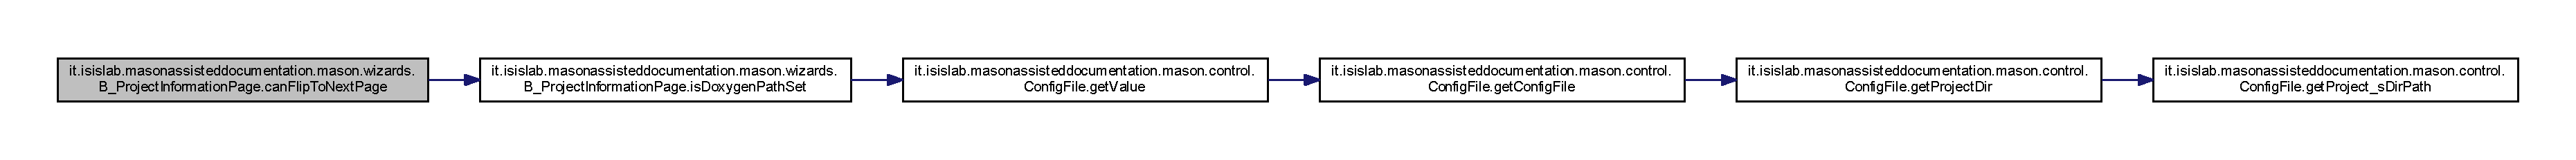
\includegraphics[width=350pt]{classit_1_1isislab_1_1masonassisteddocumentation_1_1mason_1_1wizards_1_1_b___project_information_page_a4ad2c0b1269d22b81ffc9e77f399c6af_cgraph}
\end{center}
\end{figure}




Here is the caller graph for this function\-:\nopagebreak
\begin{figure}[H]
\begin{center}
\leavevmode
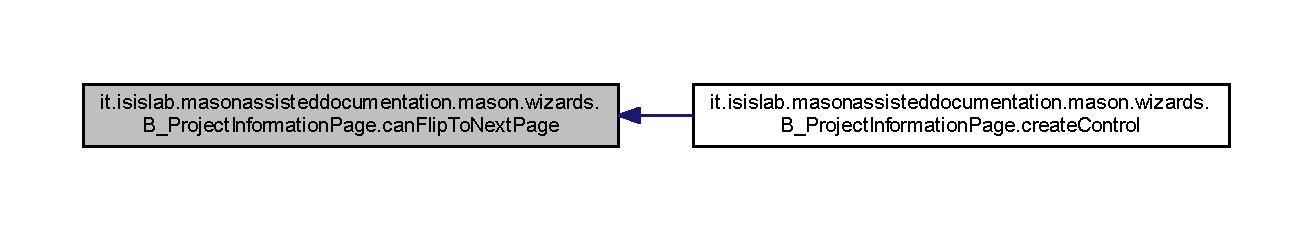
\includegraphics[width=350pt]{classit_1_1isislab_1_1masonassisteddocumentation_1_1mason_1_1wizards_1_1_b___project_information_page_a4ad2c0b1269d22b81ffc9e77f399c6af_icgraph}
\end{center}
\end{figure}


\hypertarget{classit_1_1isislab_1_1masonassisteddocumentation_1_1mason_1_1wizards_1_1_b___project_information_page_ab664591c88285aa5d3cc990620e812dd}{\index{it\-::isislab\-::masonassisteddocumentation\-::mason\-::wizards\-::\-B\-\_\-\-Project\-Information\-Page@{it\-::isislab\-::masonassisteddocumentation\-::mason\-::wizards\-::\-B\-\_\-\-Project\-Information\-Page}!create\-Control@{create\-Control}}
\index{create\-Control@{create\-Control}!it::isislab::masonassisteddocumentation::mason::wizards::B_ProjectInformationPage@{it\-::isislab\-::masonassisteddocumentation\-::mason\-::wizards\-::\-B\-\_\-\-Project\-Information\-Page}}
\subsubsection[{create\-Control}]{\setlength{\rightskip}{0pt plus 5cm}void it.\-isislab.\-masonassisteddocumentation.\-mason.\-wizards.\-B\-\_\-\-Project\-Information\-Page.\-create\-Control (
\begin{DoxyParamCaption}
\item[{Composite}]{parent}
\end{DoxyParamCaption}
)}}\label{classit_1_1isislab_1_1masonassisteddocumentation_1_1mason_1_1wizards_1_1_b___project_information_page_ab664591c88285aa5d3cc990620e812dd}

\begin{DoxyCode}
90                                                 \{
91         Composite container = \textcolor{keyword}{new} Composite(parent, SWT.NULL);
92         GridLayout layout = \textcolor{keyword}{new} GridLayout();
93         container.setLayout(layout);
94         layout.numColumns = 3;
95         layout.verticalSpacing = 9;
96         
97         Label lblOutputPath = \textcolor{keyword}{new} Label(container, SWT.NONE);
98         lblOutputPath.setLayoutData(\textcolor{keyword}{new} GridData(SWT.RIGHT, SWT.CENTER, \textcolor{keyword}{false}, \textcolor{keyword}{false}, 1, 1));
99         lblOutputPath.setText(\textcolor{stringliteral}{"Output path:"});
100         
101         \hyperlink{classit_1_1isislab_1_1masonassisteddocumentation_1_1mason_1_1wizards_1_1_b___project_information_page_aae0eab045b1d0530a794116410ae6e5d}{text} = \textcolor{keyword}{new} Text(container, SWT.BORDER);
102         text.setLayoutData(\textcolor{keyword}{new} GridData(SWT.FILL, SWT.CENTER, \textcolor{keyword}{true}, \textcolor{keyword}{false}, 1, 1));
103         text.setText(ConfigFile.getValue(\textcolor{stringliteral}{"output"}));
104         
105         \hyperlink{classit_1_1isislab_1_1masonassisteddocumentation_1_1mason_1_1wizards_1_1_b___project_information_page_a0cbfd9890c8c62af7cfce149089682b5}{btnOutputBrowse} = \textcolor{keyword}{new} Button(container, SWT.NONE);
106         btnOutputBrowse.addSelectionListener(\textcolor{keyword}{new} SelectionAdapter() \{
107             @Override
108             \textcolor{keyword}{public} \textcolor{keywordtype}{void} widgetSelected(SelectionEvent e) \{
109                 JFileChooser chooser = \textcolor{keyword}{new} JFileChooser();
110                 chooser.setCurrentDirectory(\textcolor{keyword}{new} java.io.File(\textcolor{stringliteral}{"."}));
111                 chooser.setDialogTitle(\textcolor{stringliteral}{"Browse the folder to process"});
112                 chooser.setFileSelectionMode(JFileChooser.DIRECTORIES\_ONLY);
113                 chooser.setAcceptAllFileFilterUsed(\textcolor{keyword}{false});
114                 \textcolor{keywordflow}{if} (chooser.showOpenDialog(null) == JFileChooser.APPROVE\_OPTION) \{                         
           
115                     ConfigFile.setProperty(\textcolor{stringliteral}{"output"}, chooser.getSelectedFile().getAbsolutePath());
116                     log.info(\textcolor{stringliteral}{"Config file updated: "} + chooser.getCurrentDirectory().getPath());
117                     text.setText(ConfigFile.getValue(\textcolor{stringliteral}{"output"}));
118                 \}
119             \}
120         \});
121         btnOutputBrowse.setText(\textcolor{stringliteral}{"Browse..."});
122         \hyperlink{classit_1_1isislab_1_1masonassisteddocumentation_1_1mason_1_1wizards_1_1_b___project_information_page_a4887707c3be26291594a2d0010abd500}{lblDoxygenPath} = \textcolor{keyword}{new} Label(container, SWT.NULL);
123         lblDoxygenPath.setLayoutData(\textcolor{keyword}{new} GridData(SWT.RIGHT, SWT.CENTER, \textcolor{keyword}{false}, \textcolor{keyword}{false}, 1, 1));
124         lblDoxygenPath.setText(\textcolor{stringliteral}{"Doxygen path:"});
125 
126         \hyperlink{classit_1_1isislab_1_1masonassisteddocumentation_1_1mason_1_1wizards_1_1_b___project_information_page_afd09135c84c569cc68148a0166b9390a}{containerText} = \textcolor{keyword}{new} Text(container, SWT.BORDER | SWT.SINGLE);
127         containerText.setLayoutData(\textcolor{keyword}{new} GridData(GridData.FILL\_HORIZONTAL));
128 
129         \hyperlink{classit_1_1isislab_1_1masonassisteddocumentation_1_1mason_1_1wizards_1_1_b___project_information_page_a0962e195aa316ea8c931a45b59971432}{buttonBrowse} = \textcolor{keyword}{new} Button(container, SWT.PUSH);
130         buttonBrowse.addSelectionListener(\textcolor{keyword}{new} SelectionAdapter() \{
131             @Override
132             \textcolor{keyword}{public} \textcolor{keywordtype}{void} widgetSelected(SelectionEvent e) \{
133                 JFileChooser chooser = \textcolor{keyword}{new} JFileChooser();
134                 chooser.setCurrentDirectory(\textcolor{keyword}{new} java.io.File(\textcolor{stringliteral}{"."}));
135                 chooser.setDialogTitle(\textcolor{stringliteral}{"Browse the folder to process"});
136                 chooser.setFileSelectionMode(JFileChooser.DIRECTORIES\_ONLY);
137                 chooser.setAcceptAllFileFilterUsed(\textcolor{keyword}{false});
138                 \textcolor{keywordflow}{if} (chooser.showOpenDialog(null) == JFileChooser.APPROVE\_OPTION) \{                  
139                     ConfigFile.setProperty(\textcolor{stringliteral}{"doxygenPath"}, chooser.getSelectedFile().getAbsolutePath());
140                     log.info(\textcolor{stringliteral}{"Config file updated: "} + chooser.getCurrentDirectory().getPath());
141                     \hyperlink{classit_1_1isislab_1_1masonassisteddocumentation_1_1mason_1_1wizards_1_1_b___project_information_page_ad0acda6e90aee0af403c3e9c53525b5d}{setDoxygenLabelPathFromConfig}();
142                     \hyperlink{classit_1_1isislab_1_1masonassisteddocumentation_1_1mason_1_1wizards_1_1_b___project_information_page_a4ad2c0b1269d22b81ffc9e77f399c6af}{canFlipToNextPage}();
143                 \}
144             \}
145         \});
146         buttonBrowse.setText(\textcolor{stringliteral}{"Browse..."});
147         
148         \hyperlink{classit_1_1isislab_1_1masonassisteddocumentation_1_1mason_1_1wizards_1_1_b___project_information_page_acb48412dbb797258e13404c757c8d3f4}{labelGraphvizPath} = \textcolor{keyword}{new} Label(container, SWT.NONE);
149         labelGraphvizPath.setLayoutData(\textcolor{keyword}{new} GridData(SWT.RIGHT, SWT.CENTER, \textcolor{keyword}{false}, \textcolor{keyword}{false}, 1, 1));
150         labelGraphvizPath.setText(\textcolor{stringliteral}{"Graphviz path:"});
151         
152         \hyperlink{classit_1_1isislab_1_1masonassisteddocumentation_1_1mason_1_1wizards_1_1_b___project_information_page_a03d43e1fbcdb5d7d5e6745d8f57db84b}{textGraphvizPath} = \textcolor{keyword}{new} Text(container, SWT.BORDER);
153         textGraphvizPath.setLayoutData(\textcolor{keyword}{new} GridData(SWT.FILL, SWT.CENTER, \textcolor{keyword}{true}, \textcolor{keyword}{false}, 1, 1));
154         
155         \hyperlink{classit_1_1isislab_1_1masonassisteddocumentation_1_1mason_1_1wizards_1_1_b___project_information_page_ad5db74dd5c7fc084f538fde88d57573a}{buttonGraphvizBrowser} = \textcolor{keyword}{new} Button(container, SWT.NONE);
156         buttonGraphvizBrowser.addSelectionListener(\textcolor{keyword}{new} SelectionAdapter() \{
157             @Override
158             \textcolor{keyword}{public} \textcolor{keywordtype}{void} widgetSelected(SelectionEvent e) \{
159                 JFileChooser chooser = \textcolor{keyword}{new} JFileChooser();
160                 chooser.setCurrentDirectory(\textcolor{keyword}{new} java.io.File(\textcolor{stringliteral}{"."}));
161                 chooser.setDialogTitle(\textcolor{stringliteral}{"Browse the folder to process"});
162                 chooser.setFileSelectionMode(JFileChooser.DIRECTORIES\_ONLY);
163                 chooser.setAcceptAllFileFilterUsed(\textcolor{keyword}{false});
164                 \textcolor{keywordflow}{if} (chooser.showOpenDialog(null) == JFileChooser.APPROVE\_OPTION) \{                  
165                     ConfigFile.setProperty(\textcolor{stringliteral}{"graphvizPath"}, chooser.getSelectedFile().getAbsolutePath());
166                     log.info(\textcolor{stringliteral}{"Config file updated: "} + chooser.getCurrentDirectory().getPath());
167                     textGraphvizPath.setText(ConfigFile.getValue(\textcolor{stringliteral}{"graphvizPath"}));
168                     \hyperlink{classit_1_1isislab_1_1masonassisteddocumentation_1_1mason_1_1wizards_1_1_b___project_information_page_a4ad2c0b1269d22b81ffc9e77f399c6af}{canFlipToNextPage}();
169                 \}
170             \}
171         \});
172         buttonGraphvizBrowser.setText(\textcolor{stringliteral}{"Browse..."});
173         textGraphvizPath.setText(ConfigFile.getValue(\textcolor{stringliteral}{"graphvizPath"}));;
174         
175         \hyperlink{classit_1_1isislab_1_1masonassisteddocumentation_1_1mason_1_1wizards_1_1_b___project_information_page_a6c9ce7d939e8bd032a1f2fb5e42f0d78}{lblImagePath} = \textcolor{keyword}{new} Label(container, SWT.NONE);
176         lblImagePath.setLayoutData(\textcolor{keyword}{new} GridData(SWT.RIGHT, SWT.CENTER, \textcolor{keyword}{false}, \textcolor{keyword}{false}, 1, 1));
177         lblImagePath.setText(\textcolor{stringliteral}{"Image path:"});
178         
179         \hyperlink{classit_1_1isislab_1_1masonassisteddocumentation_1_1mason_1_1wizards_1_1_b___project_information_page_a1217897a98e0714c9e7d8141b4e931d1}{textImgPath} = \textcolor{keyword}{new} Text(container, SWT.BORDER);
180         textImgPath.setLayoutData(\textcolor{keyword}{new} GridData(SWT.FILL, SWT.CENTER, \textcolor{keyword}{true}, \textcolor{keyword}{false}, 1, 1));
181         
182         \hyperlink{classit_1_1isislab_1_1masonassisteddocumentation_1_1mason_1_1wizards_1_1_b___project_information_page_a6afdf6ba02f0bf721af2acd61a2a1a5c}{btnImgBrowse} = \textcolor{keyword}{new} Button(container, SWT.NONE);
183         btnImgBrowse.addSelectionListener(\textcolor{keyword}{new} SelectionAdapter() \{
184             @Override
185             \textcolor{keyword}{public} \textcolor{keywordtype}{void} widgetSelected(SelectionEvent e) \{
186                 JFileChooser chooser = \textcolor{keyword}{new} JFileChooser();
187                 chooser.setCurrentDirectory(\textcolor{keyword}{new} java.io.File(\textcolor{stringliteral}{"."}));
188                 chooser.setDialogTitle(\textcolor{stringliteral}{"Browse the folder to process"});
189                 chooser.setFileSelectionMode(JFileChooser.DIRECTORIES\_ONLY);
190                 chooser.setAcceptAllFileFilterUsed(\textcolor{keyword}{false});
191                 \textcolor{keywordflow}{if} (chooser.showOpenDialog(null) == JFileChooser.APPROVE\_OPTION) \{                  
192                     ConfigFile.setProperty(\textcolor{stringliteral}{"imgPath"}, chooser.getSelectedFile().getAbsolutePath());
193                     log.info(\textcolor{stringliteral}{"Config file updated: "} + chooser.getCurrentDirectory().getPath());
194                     textImgPath.setText(ConfigFile.getValue(\textcolor{stringliteral}{"imgPath"}));
195                 \}
196             \}
197         \});
198         btnImgBrowse.setText(\textcolor{stringliteral}{"Browse..."});
199         textImgPath.setText(ConfigFile.getValue(\textcolor{stringliteral}{"imgPath"}));
200         \textcolor{keyword}{new} Label(container, SWT.NONE);
201         \textcolor{keyword}{new} Label(container, SWT.NONE);
202         \textcolor{keyword}{new} Label(container, SWT.NONE);
203         \textcolor{keyword}{new} Label(container, SWT.NONE);
204         
205         \hyperlink{classit_1_1isislab_1_1masonassisteddocumentation_1_1mason_1_1wizards_1_1_b___project_information_page_a89067957695a1743c11b64ff76f1e5c9}{composite\_1} = \textcolor{keyword}{new} Composite(container, SWT.NONE);
206         composite\_1.setLayout(\textcolor{keyword}{new} GridLayout(3, \textcolor{keyword}{false}));
207         GridData gd\_composite\_1 = \textcolor{keyword}{new} GridData(SWT.LEFT, SWT.CENTER, \textcolor{keyword}{false}, \textcolor{keyword}{false}, 1, 1);
208         gd\_composite\_1.widthHint = 401;
209         gd\_composite\_1.heightHint = 60;
210         composite\_1.setLayoutData(gd\_composite\_1);
211         
212         \hyperlink{classit_1_1isislab_1_1masonassisteddocumentation_1_1mason_1_1wizards_1_1_b___project_information_page_a9c18ade9b232612291e8a831823a29cf}{lblAutoColor} = \textcolor{keyword}{new} Label(\hyperlink{classit_1_1isislab_1_1masonassisteddocumentation_1_1mason_1_1wizards_1_1_b___project_information_page_a89067957695a1743c11b64ff76f1e5c9}{composite\_1}, SWT.NONE);
213         lblAutoColor.setLayoutData(\textcolor{keyword}{new} GridData(SWT.RIGHT, SWT.CENTER, \textcolor{keyword}{false}, \textcolor{keyword}{false}, 1, 1));
214         lblAutoColor.setText(\textcolor{stringliteral}{"Auto-generated info color:"});
215 
216         
217         \textcolor{keyword}{final} RGB autoRGB = \textcolor{keyword}{new} RGB(32, 1, 205);    \textcolor{comment}{//default blue}
218         \textcolor{keywordflow}{if} (!ConfigFile.getValue(\textcolor{stringliteral}{"R\_Value\_auto"}).equals(\textcolor{stringliteral}{""}) && !ConfigFile.getValue(\textcolor{stringliteral}{"G\_Value\_auto"}).equals(\textcolor{stringliteral}{
      ""}) && !ConfigFile.getValue(\textcolor{stringliteral}{"B\_Value\_auto"}).equals(\textcolor{stringliteral}{""}))\{
219             autoRGB.red = Integer.parseInt(ConfigFile.getValue(\textcolor{stringliteral}{"R\_Value\_auto"}));
220             autoRGB.green = Integer.parseInt(ConfigFile.getValue(\textcolor{stringliteral}{"G\_Value\_auto"}));
221             autoRGB.blue = Integer.parseInt(ConfigFile.getValue(\textcolor{stringliteral}{"B\_Value\_auto"}));       
222             GlobalUtility.autoOutputColor[0] = autoRGB.red;
223             GlobalUtility.autoOutputColor[1] = autoRGB.green;
224             GlobalUtility.autoOutputColor[2] = autoRGB.blue;
225         \}
226         \hyperlink{classit_1_1isislab_1_1masonassisteddocumentation_1_1mason_1_1wizards_1_1_b___project_information_page_a1c3cf5ff2d1b0d408f03db81e8e40c6a}{btnAutoColor} = \textcolor{keyword}{new} Button(\hyperlink{classit_1_1isislab_1_1masonassisteddocumentation_1_1mason_1_1wizards_1_1_b___project_information_page_a89067957695a1743c11b64ff76f1e5c9}{composite\_1}, SWT.NONE);
227         btnAutoColor.setText(\textcolor{stringliteral}{"Choose"});
228         \hyperlink{classit_1_1isislab_1_1masonassisteddocumentation_1_1mason_1_1wizards_1_1_b___project_information_page_ae3ce9b9ca6502f09db614860f5a1a127}{lblViewAutoColor} = \textcolor{keyword}{new} Label(\hyperlink{classit_1_1isislab_1_1masonassisteddocumentation_1_1mason_1_1wizards_1_1_b___project_information_page_a89067957695a1743c11b64ff76f1e5c9}{composite\_1}, SWT.NONE);
229         lblViewAutoColor.setForeground(SWTResourceManager.getColor(autoRGB));
230         lblViewAutoColor.setText(\textcolor{stringliteral}{"AAAAA"});
231         lblViewAutoColor.setBackground(SWTResourceManager.getColor(autoRGB));
232         btnAutoColor.addSelectionListener(\textcolor{keyword}{new} SelectionAdapter() \{
233             @Override
234             \textcolor{keyword}{public} \textcolor{keywordtype}{void} widgetSelected(SelectionEvent e) \{
235                 Color c = JColorChooser.showDialog(null, \textcolor{stringliteral}{"Choose a Color"}, null);
236                   \textcolor{keywordflow}{if} (c != null)\{
237                       autoRGB.red = c.getRed();
238                       autoRGB.green = c.getGreen();
239                       autoRGB.blue = c.getBlue();
240                       lblViewAutoColor.setForeground(SWTResourceManager.getColor(autoRGB));
241                       lblViewAutoColor.setBackground(SWTResourceManager.getColor(autoRGB));
242                       GlobalUtility.autoOutputColor[0] = c.getRed();
243                       GlobalUtility.autoOutputColor[1] = c.getGreen();
244                       GlobalUtility.autoOutputColor[2] = c.getBlue();
245                       ConfigFile.setProperty(\textcolor{stringliteral}{"R\_Value\_auto"}, c.getRed()+\textcolor{stringliteral}{""});
246                       ConfigFile.setProperty(\textcolor{stringliteral}{"G\_Value\_auto"}, c.getGreen()+\textcolor{stringliteral}{""});
247                       ConfigFile.setProperty(\textcolor{stringliteral}{"B\_Value\_auto"}, c.getBlue()+\textcolor{stringliteral}{""});
248                   \}
249                 \}
250             \});
251         
252         
253         \hyperlink{classit_1_1isislab_1_1masonassisteddocumentation_1_1mason_1_1wizards_1_1_b___project_information_page_a0cc1d0856402dfcda75702e789c68733}{labelUserColor} = \textcolor{keyword}{new} Label(\hyperlink{classit_1_1isislab_1_1masonassisteddocumentation_1_1mason_1_1wizards_1_1_b___project_information_page_a89067957695a1743c11b64ff76f1e5c9}{composite\_1}, SWT.RIGHT);
254         labelUserColor.setLayoutData(\textcolor{keyword}{new} GridData(SWT.RIGHT, SWT.CENTER, \textcolor{keyword}{false}, \textcolor{keyword}{false}, 1, 1));
255         labelUserColor.setText(\textcolor{stringliteral}{"User info color:"});
256         
257         \textcolor{keyword}{final} RGB userRGB = \textcolor{keyword}{new} RGB(0, 0, 0);   \textcolor{comment}{//default black}
258         \textcolor{keywordflow}{if} (!ConfigFile.getValue(\textcolor{stringliteral}{"R\_Value\_user"}).equals(\textcolor{stringliteral}{""}) && !ConfigFile.getValue(\textcolor{stringliteral}{"G\_Value\_user"}).equals(\textcolor{stringliteral}{
      ""}) && !ConfigFile.getValue(\textcolor{stringliteral}{"B\_Value\_user"}).equals(\textcolor{stringliteral}{""}))\{
259             userRGB.red = Integer.parseInt(ConfigFile.getValue(\textcolor{stringliteral}{"R\_Value\_user"}));
260             userRGB.green = Integer.parseInt(ConfigFile.getValue(\textcolor{stringliteral}{"G\_Value\_user"}));
261             userRGB.blue = Integer.parseInt(ConfigFile.getValue(\textcolor{stringliteral}{"B\_Value\_user"}));
262             GlobalUtility.userOutputColor[0] = userRGB.red;
263             GlobalUtility.userOutputColor[1] = userRGB.green;
264             GlobalUtility.userOutputColor[2] = userRGB.blue;
265         \}
266         \hyperlink{classit_1_1isislab_1_1masonassisteddocumentation_1_1mason_1_1wizards_1_1_b___project_information_page_a0c0c20817602a22ba74f88744083be6b}{btnUserColor} = \textcolor{keyword}{new} Button(\hyperlink{classit_1_1isislab_1_1masonassisteddocumentation_1_1mason_1_1wizards_1_1_b___project_information_page_a89067957695a1743c11b64ff76f1e5c9}{composite\_1}, SWT.NONE);
267         \hyperlink{classit_1_1isislab_1_1masonassisteddocumentation_1_1mason_1_1wizards_1_1_b___project_information_page_abf3d5350bf4a246805afb445ef49380a}{lblViewUserColor} = \textcolor{keyword}{new} Label(\hyperlink{classit_1_1isislab_1_1masonassisteddocumentation_1_1mason_1_1wizards_1_1_b___project_information_page_a89067957695a1743c11b64ff76f1e5c9}{composite\_1}, SWT.NONE);
268         lblViewUserColor.setText(\textcolor{stringliteral}{"AAAAA"});
269         lblViewUserColor.setForeground(SWTResourceManager.getColor(userRGB));
270         lblViewUserColor.setBackground(SWTResourceManager.getColor(userRGB));
271         btnUserColor.addSelectionListener(\textcolor{keyword}{new} SelectionAdapter() \{
272             @Override
273             \textcolor{keyword}{public} \textcolor{keywordtype}{void} widgetSelected(SelectionEvent e) \{
274                 Color c = JColorChooser.showDialog(null, \textcolor{stringliteral}{"Choose a Color"}, null);
275                   \textcolor{keywordflow}{if} (c != null)\{
276                       userRGB.red = c.getRed();
277                       userRGB.green = c.getGreen();
278                       userRGB.blue = c.getBlue();
279                       lblViewUserColor.setForeground(SWTResourceManager.getColor(userRGB));
280                       lblViewUserColor.setBackground(SWTResourceManager.getColor(userRGB));
281                       GlobalUtility.userOutputColor[0] = c.getRed();
282                       GlobalUtility.userOutputColor[1] = c.getGreen();
283                       GlobalUtility.userOutputColor[2] = c.getBlue();
284                       ConfigFile.setProperty(\textcolor{stringliteral}{"R\_Value\_user"}, c.getRed()+\textcolor{stringliteral}{""});
285                       ConfigFile.setProperty(\textcolor{stringliteral}{"G\_Value\_user"}, c.getGreen()+\textcolor{stringliteral}{""});
286                       ConfigFile.setProperty(\textcolor{stringliteral}{"B\_Value\_user"}, c.getBlue()+\textcolor{stringliteral}{""});
287                   \}
288             \}
289         \});
290         btnUserColor.setText(\textcolor{stringliteral}{"Choose"});
291         
292         
293         \textcolor{keyword}{new} Label(container, SWT.NONE);
294         \textcolor{keyword}{new} Label(container, SWT.NONE);
295         
296         \hyperlink{classit_1_1isislab_1_1masonassisteddocumentation_1_1mason_1_1wizards_1_1_b___project_information_page_a08c0494b74656d068e78bbe0a56715ed}{label\_Message} = \textcolor{keyword}{new} Label(container, SWT.NONE);
297         label\_Message.setText(\textcolor{stringliteral}{""});
298         \textcolor{keyword}{new} Label(container, SWT.NONE);
299         \textcolor{keyword}{new} Label(container, SWT.NONE);
300         
301         \hyperlink{classit_1_1isislab_1_1masonassisteddocumentation_1_1mason_1_1wizards_1_1_b___project_information_page_adf33db8f408e4f486a256d199eae3bae}{scrolledComposite} = \textcolor{keyword}{new} ScrolledComposite(container, SWT.BORDER | SWT.H\_SCROLL | 
      SWT.V\_SCROLL);
302         GridData gd\_scrolledComposite = \textcolor{keyword}{new} GridData(SWT.LEFT, SWT.CENTER, \textcolor{keyword}{false}, \textcolor{keyword}{false}, 1, 1);
303         gd\_scrolledComposite.heightHint = 75;
304         gd\_scrolledComposite.widthHint = 384;
305         scrolledComposite.setLayoutData(gd\_scrolledComposite);
306         scrolledComposite.setExpandHorizontal(\textcolor{keyword}{true});
307         scrolledComposite.setExpandVertical(\textcolor{keyword}{true});
308         
309         \hyperlink{classit_1_1isislab_1_1masonassisteddocumentation_1_1mason_1_1wizards_1_1_b___project_information_page_abff2b9b46293282381b6cd1b26f83792}{composite} = \textcolor{keyword}{new} Composite(\hyperlink{classit_1_1isislab_1_1masonassisteddocumentation_1_1mason_1_1wizards_1_1_b___project_information_page_adf33db8f408e4f486a256d199eae3bae}{scrolledComposite}, SWT.NONE);
310         composite.setLayout(\textcolor{keyword}{new} GridLayout(1, \textcolor{keyword}{false}));
311         
312         \textcolor{keywordflow}{if} (\hyperlink{classit_1_1isislab_1_1masonassisteddocumentation_1_1mason_1_1wizards_1_1_b___project_information_page_a5129feb0fa34a1d51e44a2fe495ac42c}{projectAnalizer}.\hyperlink{classit_1_1isislab_1_1masonassisteddocumentation_1_1mason_1_1analizer_1_1_project_analizer_ae6fe885ccc66aeb5c5d5ba6d09ed893c}{isMasonProject}())\{
313             \hyperlink{classit_1_1isislab_1_1masonassisteddocumentation_1_1mason_1_1wizards_1_1_b___project_information_page_af5afa21c1d0087572ad8b3d0a1a1fe9c}{setProjectLabel}();
314         \}
315         scrolledComposite.setContent(\hyperlink{classit_1_1isislab_1_1masonassisteddocumentation_1_1mason_1_1wizards_1_1_b___project_information_page_abff2b9b46293282381b6cd1b26f83792}{composite});
316         scrolledComposite.setMinSize(composite.computeSize(SWT.DEFAULT, SWT.DEFAULT));
317         \textcolor{keyword}{new} Label(container, SWT.NONE);
318         setControl(container);
319         
320         \hyperlink{classit_1_1isislab_1_1masonassisteddocumentation_1_1mason_1_1wizards_1_1_b___project_information_page_ad0acda6e90aee0af403c3e9c53525b5d}{setDoxygenLabelPathFromConfig}();
321         \textcolor{keywordflow}{if} (!\hyperlink{classit_1_1isislab_1_1masonassisteddocumentation_1_1mason_1_1wizards_1_1_b___project_information_page_a5129feb0fa34a1d51e44a2fe495ac42c}{projectAnalizer}.\hyperlink{classit_1_1isislab_1_1masonassisteddocumentation_1_1mason_1_1analizer_1_1_project_analizer_ae6fe885ccc66aeb5c5d5ba6d09ed893c}{isMasonProject}()) 
      \hyperlink{classit_1_1isislab_1_1masonassisteddocumentation_1_1mason_1_1wizards_1_1_b___project_information_page_a08c0494b74656d068e78bbe0a56715ed}{label\_Message}.setText(\textcolor{stringliteral}{"Please select a project that use MASON library!"});
322         \textcolor{keywordflow}{if} (\hyperlink{classit_1_1isislab_1_1masonassisteddocumentation_1_1mason_1_1wizards_1_1_b___project_information_page_a5b4f818a204c8f8a1934ceaf016cabd7}{isDoxygenPathSet}() && \hyperlink{classit_1_1isislab_1_1masonassisteddocumentation_1_1mason_1_1wizards_1_1_b___project_information_page_a5129feb0fa34a1d51e44a2fe495ac42c}{projectAnalizer}.
      \hyperlink{classit_1_1isislab_1_1masonassisteddocumentation_1_1mason_1_1analizer_1_1_project_analizer_ae6fe885ccc66aeb5c5d5ba6d09ed893c}{isMasonProject}()) super.setPageComplete(\textcolor{keyword}{true});
323         \textcolor{keywordflow}{else}    super.setPageComplete(\textcolor{keyword}{false});
324         
325         \textcolor{comment}{//What we can see?}
326         String typeOutput = ConfigFile.getValue(\textcolor{stringliteral}{"typeOutput"});
327         \textcolor{keywordflow}{if} (typeOutput.equals(\textcolor{stringliteral}{"pdf"}))\{
328             lblDoxygenPath.setVisible(\textcolor{keyword}{false});
329             labelGraphvizPath.setVisible(\textcolor{keyword}{false});
330             lblAutoColor.setVisible(\textcolor{keyword}{false});
331             labelUserColor.setVisible(\textcolor{keyword}{false});
332             containerText.setVisible(\textcolor{keyword}{false});
333             textGraphvizPath.setVisible(\textcolor{keyword}{false});
334             btnAutoColor.setVisible(\textcolor{keyword}{false});
335             btnUserColor.setVisible(\textcolor{keyword}{false});
336             buttonBrowse.setVisible(\textcolor{keyword}{false});
337             buttonGraphvizBrowser.setVisible(\textcolor{keyword}{false});
338             lblViewAutoColor.setVisible(\textcolor{keyword}{false});
339             lblViewUserColor.setVisible(\textcolor{keyword}{false});
340         \}
341         \textcolor{keywordflow}{if} (typeOutput.equals(\textcolor{stringliteral}{"txt"}))\{
342             lblDoxygenPath.setVisible(\textcolor{keyword}{false});
343             labelGraphvizPath.setVisible(\textcolor{keyword}{false});
344             lblAutoColor.setVisible(\textcolor{keyword}{false});
345             labelUserColor.setVisible(\textcolor{keyword}{false});
346             lblImagePath.setVisible(\textcolor{keyword}{false});
347             containerText.setVisible(\textcolor{keyword}{false});
348             textGraphvizPath.setVisible(\textcolor{keyword}{false});
349             textImgPath.setVisible(\textcolor{keyword}{false});
350             btnAutoColor.setVisible(\textcolor{keyword}{false});
351             btnUserColor.setVisible(\textcolor{keyword}{false});
352             btnImgBrowse.setVisible(\textcolor{keyword}{false});
353             buttonBrowse.setVisible(\textcolor{keyword}{false});
354             buttonGraphvizBrowser.setVisible(\textcolor{keyword}{false});
355             lblViewAutoColor.setVisible(\textcolor{keyword}{false});
356             lblViewUserColor.setVisible(\textcolor{keyword}{false});
357         \}   
358     \}
\end{DoxyCode}


Here is the call graph for this function\-:\nopagebreak
\begin{figure}[H]
\begin{center}
\leavevmode
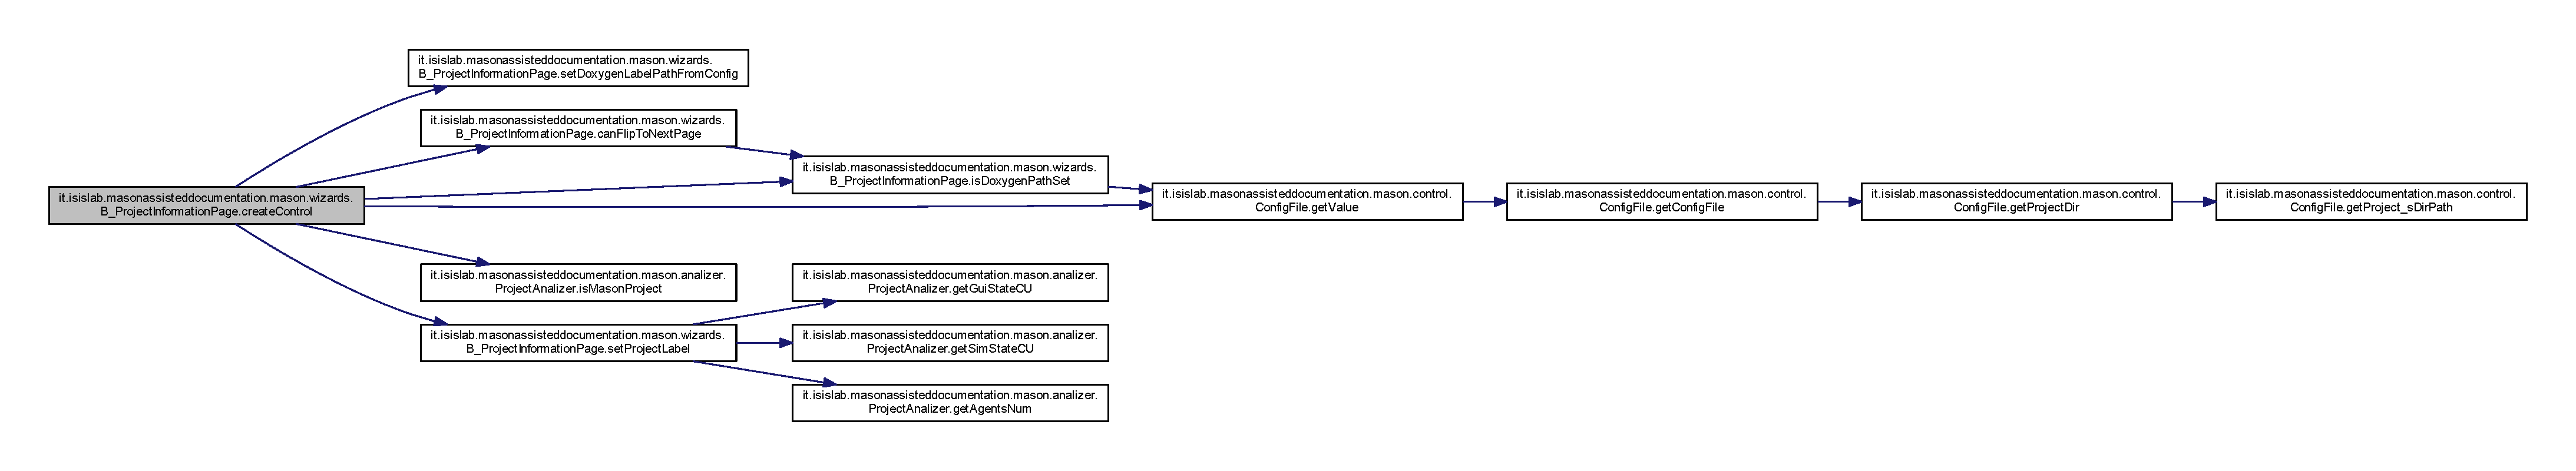
\includegraphics[width=350pt]{classit_1_1isislab_1_1masonassisteddocumentation_1_1mason_1_1wizards_1_1_b___project_information_page_ab664591c88285aa5d3cc990620e812dd_cgraph}
\end{center}
\end{figure}


\hypertarget{classit_1_1isislab_1_1masonassisteddocumentation_1_1mason_1_1wizards_1_1_b___project_information_page_a62abef1230b2c72e555e530004e4c5f9}{\index{it\-::isislab\-::masonassisteddocumentation\-::mason\-::wizards\-::\-B\-\_\-\-Project\-Information\-Page@{it\-::isislab\-::masonassisteddocumentation\-::mason\-::wizards\-::\-B\-\_\-\-Project\-Information\-Page}!get\-Next\-Page@{get\-Next\-Page}}
\index{get\-Next\-Page@{get\-Next\-Page}!it::isislab::masonassisteddocumentation::mason::wizards::B_ProjectInformationPage@{it\-::isislab\-::masonassisteddocumentation\-::mason\-::wizards\-::\-B\-\_\-\-Project\-Information\-Page}}
\subsubsection[{get\-Next\-Page}]{\setlength{\rightskip}{0pt plus 5cm}I\-Wizard\-Page it.\-isislab.\-masonassisteddocumentation.\-mason.\-wizards.\-B\-\_\-\-Project\-Information\-Page.\-get\-Next\-Page (
\begin{DoxyParamCaption}
{}
\end{DoxyParamCaption}
)}}\label{classit_1_1isislab_1_1masonassisteddocumentation_1_1mason_1_1wizards_1_1_b___project_information_page_a62abef1230b2c72e555e530004e4c5f9}

\begin{DoxyCode}
395                                     \{ 
396         C\_PurposePage nextPage = \textcolor{keyword}{new} C\_PurposePage();
397         ((MASONDocumentationWizard) super.getWizard()).addPage(nextPage);
398         \textcolor{keywordflow}{return} nextPage;
399     \}
\end{DoxyCode}
\hypertarget{classit_1_1isislab_1_1masonassisteddocumentation_1_1mason_1_1wizards_1_1_b___project_information_page_a5b4f818a204c8f8a1934ceaf016cabd7}{\index{it\-::isislab\-::masonassisteddocumentation\-::mason\-::wizards\-::\-B\-\_\-\-Project\-Information\-Page@{it\-::isislab\-::masonassisteddocumentation\-::mason\-::wizards\-::\-B\-\_\-\-Project\-Information\-Page}!is\-Doxygen\-Path\-Set@{is\-Doxygen\-Path\-Set}}
\index{is\-Doxygen\-Path\-Set@{is\-Doxygen\-Path\-Set}!it::isislab::masonassisteddocumentation::mason::wizards::B_ProjectInformationPage@{it\-::isislab\-::masonassisteddocumentation\-::mason\-::wizards\-::\-B\-\_\-\-Project\-Information\-Page}}
\subsubsection[{is\-Doxygen\-Path\-Set}]{\setlength{\rightskip}{0pt plus 5cm}boolean it.\-isislab.\-masonassisteddocumentation.\-mason.\-wizards.\-B\-\_\-\-Project\-Information\-Page.\-is\-Doxygen\-Path\-Set (
\begin{DoxyParamCaption}
{}
\end{DoxyParamCaption}
)}}\label{classit_1_1isislab_1_1masonassisteddocumentation_1_1mason_1_1wizards_1_1_b___project_information_page_a5b4f818a204c8f8a1934ceaf016cabd7}
Check if Doxygen path is set \begin{DoxyReturn}{Returns}
true if Doxygen path is set 
\end{DoxyReturn}

\begin{DoxyCode}
86                                      \{
87         \textcolor{keywordflow}{return} (ConfigFile.getValue(\textcolor{stringliteral}{"doxygenPath"})!=null);
88     \}
\end{DoxyCode}


Here is the call graph for this function\-:\nopagebreak
\begin{figure}[H]
\begin{center}
\leavevmode
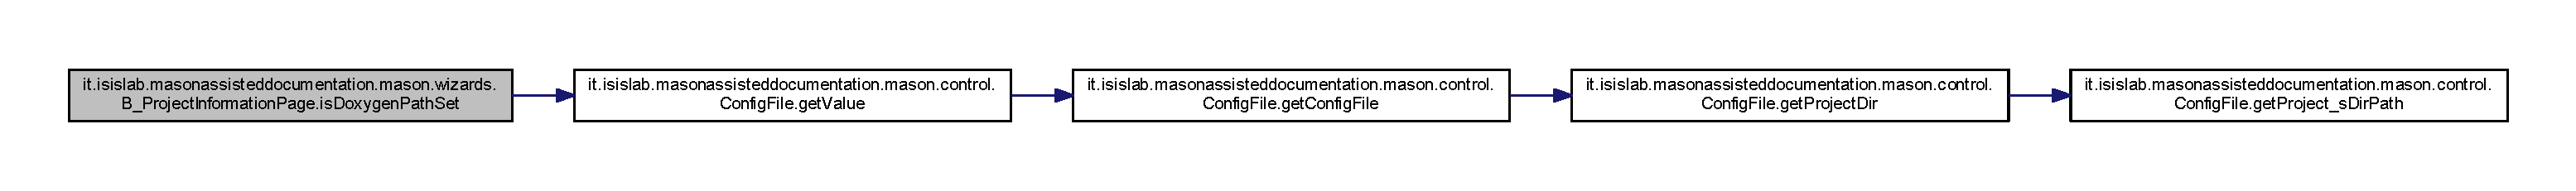
\includegraphics[width=350pt]{classit_1_1isislab_1_1masonassisteddocumentation_1_1mason_1_1wizards_1_1_b___project_information_page_a5b4f818a204c8f8a1934ceaf016cabd7_cgraph}
\end{center}
\end{figure}




Here is the caller graph for this function\-:\nopagebreak
\begin{figure}[H]
\begin{center}
\leavevmode
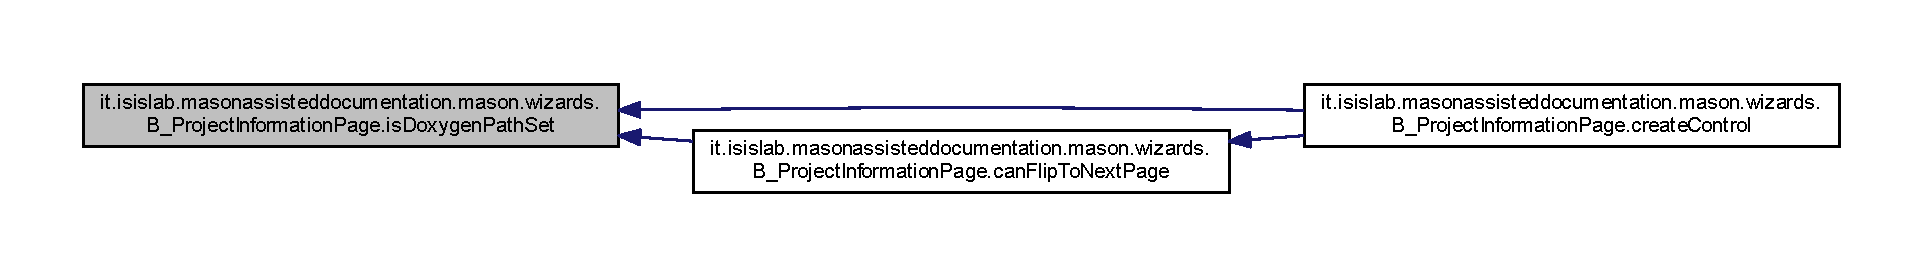
\includegraphics[width=350pt]{classit_1_1isislab_1_1masonassisteddocumentation_1_1mason_1_1wizards_1_1_b___project_information_page_a5b4f818a204c8f8a1934ceaf016cabd7_icgraph}
\end{center}
\end{figure}


\hypertarget{classit_1_1isislab_1_1masonassisteddocumentation_1_1mason_1_1wizards_1_1_b___project_information_page_a86f79621a6b3201e70a35c54ec1e8c3f}{\index{it\-::isislab\-::masonassisteddocumentation\-::mason\-::wizards\-::\-B\-\_\-\-Project\-Information\-Page@{it\-::isislab\-::masonassisteddocumentation\-::mason\-::wizards\-::\-B\-\_\-\-Project\-Information\-Page}!is\-Page\-Complete@{is\-Page\-Complete}}
\index{is\-Page\-Complete@{is\-Page\-Complete}!it::isislab::masonassisteddocumentation::mason::wizards::B_ProjectInformationPage@{it\-::isislab\-::masonassisteddocumentation\-::mason\-::wizards\-::\-B\-\_\-\-Project\-Information\-Page}}
\subsubsection[{is\-Page\-Complete}]{\setlength{\rightskip}{0pt plus 5cm}boolean it.\-isislab.\-masonassisteddocumentation.\-mason.\-wizards.\-B\-\_\-\-Project\-Information\-Page.\-is\-Page\-Complete (
\begin{DoxyParamCaption}
{}
\end{DoxyParamCaption}
)}}\label{classit_1_1isislab_1_1masonassisteddocumentation_1_1mason_1_1wizards_1_1_b___project_information_page_a86f79621a6b3201e70a35c54ec1e8c3f}

\begin{DoxyCode}
391                                    \{
392         \textcolor{keywordflow}{return} \textcolor{keyword}{true};
393     \}
\end{DoxyCode}
\hypertarget{classit_1_1isislab_1_1masonassisteddocumentation_1_1mason_1_1wizards_1_1_b___project_information_page_ad0acda6e90aee0af403c3e9c53525b5d}{\index{it\-::isislab\-::masonassisteddocumentation\-::mason\-::wizards\-::\-B\-\_\-\-Project\-Information\-Page@{it\-::isislab\-::masonassisteddocumentation\-::mason\-::wizards\-::\-B\-\_\-\-Project\-Information\-Page}!set\-Doxygen\-Label\-Path\-From\-Config@{set\-Doxygen\-Label\-Path\-From\-Config}}
\index{set\-Doxygen\-Label\-Path\-From\-Config@{set\-Doxygen\-Label\-Path\-From\-Config}!it::isislab::masonassisteddocumentation::mason::wizards::B_ProjectInformationPage@{it\-::isislab\-::masonassisteddocumentation\-::mason\-::wizards\-::\-B\-\_\-\-Project\-Information\-Page}}
\subsubsection[{set\-Doxygen\-Label\-Path\-From\-Config}]{\setlength{\rightskip}{0pt plus 5cm}void it.\-isislab.\-masonassisteddocumentation.\-mason.\-wizards.\-B\-\_\-\-Project\-Information\-Page.\-set\-Doxygen\-Label\-Path\-From\-Config (
\begin{DoxyParamCaption}
{}
\end{DoxyParamCaption}
)\hspace{0.3cm}{\ttfamily [private]}}}\label{classit_1_1isislab_1_1masonassisteddocumentation_1_1mason_1_1wizards_1_1_b___project_information_page_ad0acda6e90aee0af403c3e9c53525b5d}

\begin{DoxyCode}
77                                                  \{
78         this.containerText.setText(ConfigFile.getValue(\textcolor{stringliteral}{"doxygenPath"}));
79         log.info(\textcolor{stringliteral}{"doxygenPath text update\(\backslash\)n"} + this.containerText.getText());
80     \}
\end{DoxyCode}


Here is the caller graph for this function\-:\nopagebreak
\begin{figure}[H]
\begin{center}
\leavevmode
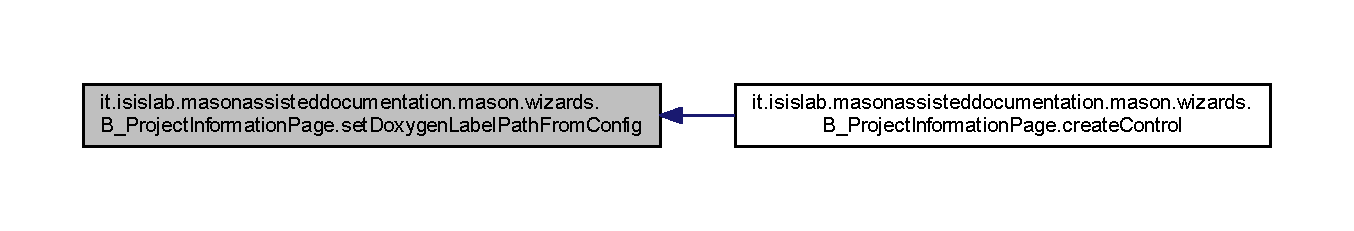
\includegraphics[width=350pt]{classit_1_1isislab_1_1masonassisteddocumentation_1_1mason_1_1wizards_1_1_b___project_information_page_ad0acda6e90aee0af403c3e9c53525b5d_icgraph}
\end{center}
\end{figure}


\hypertarget{classit_1_1isislab_1_1masonassisteddocumentation_1_1mason_1_1wizards_1_1_b___project_information_page_af5afa21c1d0087572ad8b3d0a1a1fe9c}{\index{it\-::isislab\-::masonassisteddocumentation\-::mason\-::wizards\-::\-B\-\_\-\-Project\-Information\-Page@{it\-::isislab\-::masonassisteddocumentation\-::mason\-::wizards\-::\-B\-\_\-\-Project\-Information\-Page}!set\-Project\-Label@{set\-Project\-Label}}
\index{set\-Project\-Label@{set\-Project\-Label}!it::isislab::masonassisteddocumentation::mason::wizards::B_ProjectInformationPage@{it\-::isislab\-::masonassisteddocumentation\-::mason\-::wizards\-::\-B\-\_\-\-Project\-Information\-Page}}
\subsubsection[{set\-Project\-Label}]{\setlength{\rightskip}{0pt plus 5cm}void it.\-isislab.\-masonassisteddocumentation.\-mason.\-wizards.\-B\-\_\-\-Project\-Information\-Page.\-set\-Project\-Label (
\begin{DoxyParamCaption}
{}
\end{DoxyParamCaption}
)\hspace{0.3cm}{\ttfamily [private]}}}\label{classit_1_1isislab_1_1masonassisteddocumentation_1_1mason_1_1wizards_1_1_b___project_information_page_af5afa21c1d0087572ad8b3d0a1a1fe9c}

\begin{DoxyCode}
360                                    \{
361         \hyperlink{classit_1_1isislab_1_1masonassisteddocumentation_1_1mason_1_1wizards_1_1_b___project_information_page_a801e6444bc2096376ffbfd62f2660aaf}{lblProjectFound} = \textcolor{keyword}{new} Label(\hyperlink{classit_1_1isislab_1_1masonassisteddocumentation_1_1mason_1_1wizards_1_1_b___project_information_page_abff2b9b46293282381b6cd1b26f83792}{composite}, SWT.NONE);
362         lblProjectFound.setText(\textcolor{stringliteral}{"Project Found: "} + projectAnalizer.getProjectName());
363         \textcolor{keywordflow}{if} (\hyperlink{classit_1_1isislab_1_1masonassisteddocumentation_1_1mason_1_1wizards_1_1_b___project_information_page_a5129feb0fa34a1d51e44a2fe495ac42c}{projectAnalizer}.\hyperlink{classit_1_1isislab_1_1masonassisteddocumentation_1_1mason_1_1analizer_1_1_project_analizer_a9ba560ab2eabd5887414df46aedc1762}{getGuiStateCU}()!=null)
364             \textcolor{keywordflow}{if} (\hyperlink{classit_1_1isislab_1_1masonassisteddocumentation_1_1mason_1_1wizards_1_1_b___project_information_page_a5129feb0fa34a1d51e44a2fe495ac42c}{projectAnalizer}.\hyperlink{classit_1_1isislab_1_1masonassisteddocumentation_1_1mason_1_1analizer_1_1_project_analizer_a9ba560ab2eabd5887414df46aedc1762}{getGuiStateCU}().getElementName()!=null)\{
365                 \hyperlink{classit_1_1isislab_1_1masonassisteddocumentation_1_1mason_1_1wizards_1_1_b___project_information_page_a65bb7c12ddee14a56433fb0af2e97e89}{lblGuiState} = \textcolor{keyword}{new} Label(\hyperlink{classit_1_1isislab_1_1masonassisteddocumentation_1_1mason_1_1wizards_1_1_b___project_information_page_abff2b9b46293282381b6cd1b26f83792}{composite}, SWT.NONE);
366                 lblGuiState.setText(\textcolor{stringliteral}{"GUISTATE: "} + projectAnalizer.getGuiStateCU().getElementName());
367             \}
368         \textcolor{keywordflow}{else}
369             lblGuiState.setText(\textcolor{stringliteral}{"GUI not found"});   
370         \hyperlink{classit_1_1isislab_1_1masonassisteddocumentation_1_1mason_1_1wizards_1_1_b___project_information_page_aa7b41a14af9155e5feaff4060af3a2c4}{lblSimState} = \textcolor{keyword}{new} Label(\hyperlink{classit_1_1isislab_1_1masonassisteddocumentation_1_1mason_1_1wizards_1_1_b___project_information_page_abff2b9b46293282381b6cd1b26f83792}{composite}, SWT.NONE);
371         \textcolor{keywordflow}{if} (\hyperlink{classit_1_1isislab_1_1masonassisteddocumentation_1_1mason_1_1wizards_1_1_b___project_information_page_a5129feb0fa34a1d51e44a2fe495ac42c}{projectAnalizer}.\hyperlink{classit_1_1isislab_1_1masonassisteddocumentation_1_1mason_1_1analizer_1_1_project_analizer_aab153a7017dc5c1941d353be201491c3}{getSimStateCU}() != null)
372             lblSimState.setText(\textcolor{stringliteral}{"SIMSTATE: "} + \hyperlink{classit_1_1isislab_1_1masonassisteddocumentation_1_1mason_1_1wizards_1_1_b___project_information_page_a5129feb0fa34a1d51e44a2fe495ac42c}{projectAnalizer}.
      \hyperlink{classit_1_1isislab_1_1masonassisteddocumentation_1_1mason_1_1analizer_1_1_project_analizer_aab153a7017dc5c1941d353be201491c3}{getSimStateCU}().getElementName());
373         \textcolor{keywordflow}{else}\{
374             JOptionPane.showMessageDialog(null, \textcolor{stringliteral}{"Project doesn't contain SimState Class!"});
375             log.severe(\textcolor{stringliteral}{"Select project doesn't contain SimState Class!"});
376             System.exit(1);;
377         \}           
378         \textcolor{keywordflow}{if} (\hyperlink{classit_1_1isislab_1_1masonassisteddocumentation_1_1mason_1_1wizards_1_1_b___project_information_page_a5129feb0fa34a1d51e44a2fe495ac42c}{projectAnalizer}.\hyperlink{classit_1_1isislab_1_1masonassisteddocumentation_1_1mason_1_1analizer_1_1_project_analizer_aac2a739694623fe15e566ca0330bce3c}{getAgentsNum}()!=0)\{
379             \hyperlink{classit_1_1isislab_1_1masonassisteddocumentation_1_1mason_1_1wizards_1_1_b___project_information_page_af5b4ee969085257cfe8a66867d217b8d}{lblAgent} = \textcolor{keyword}{new} Label(\hyperlink{classit_1_1isislab_1_1masonassisteddocumentation_1_1mason_1_1wizards_1_1_b___project_information_page_abff2b9b46293282381b6cd1b26f83792}{composite}, SWT.NONE);
380             \textcolor{keywordflow}{for} (\textcolor{keywordtype}{int} i=0; i<projectAnalizer.getAgentsNum(); i++)
381                 \hyperlink{classit_1_1isislab_1_1masonassisteddocumentation_1_1mason_1_1wizards_1_1_b___project_information_page_af5b4ee969085257cfe8a66867d217b8d}{lblAgent}.setText(\hyperlink{classit_1_1isislab_1_1masonassisteddocumentation_1_1mason_1_1wizards_1_1_b___project_information_page_af5b4ee969085257cfe8a66867d217b8d}{lblAgent}.getText() + \textcolor{stringliteral}{"AGENT: "} + 
      projectAnalizer.getAgentCU(i).getElementName() +\textcolor{stringliteral}{"\(\backslash\)n"});
382         \}
383     \}
\end{DoxyCode}


Here is the call graph for this function\-:\nopagebreak
\begin{figure}[H]
\begin{center}
\leavevmode
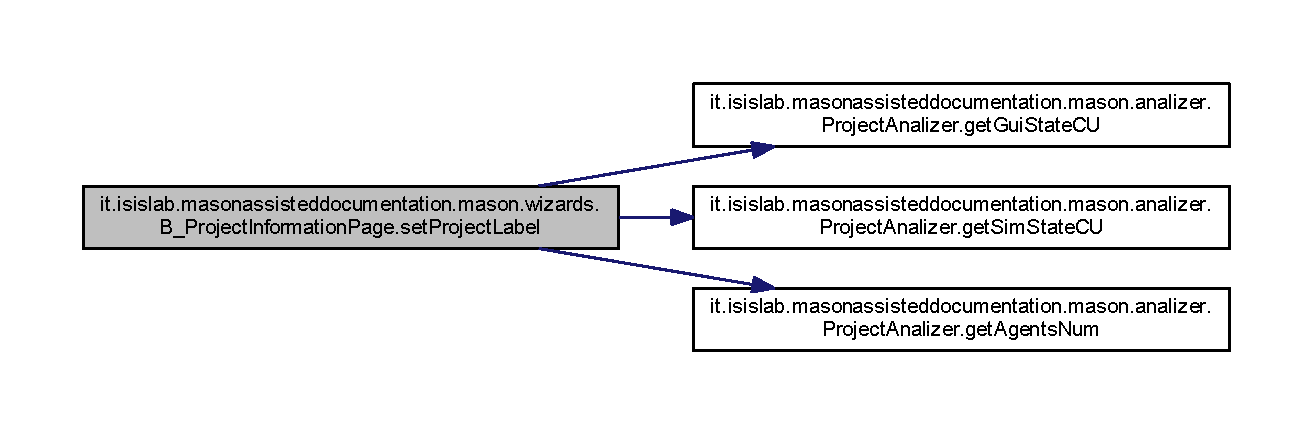
\includegraphics[width=350pt]{classit_1_1isislab_1_1masonassisteddocumentation_1_1mason_1_1wizards_1_1_b___project_information_page_af5afa21c1d0087572ad8b3d0a1a1fe9c_cgraph}
\end{center}
\end{figure}




Here is the caller graph for this function\-:\nopagebreak
\begin{figure}[H]
\begin{center}
\leavevmode
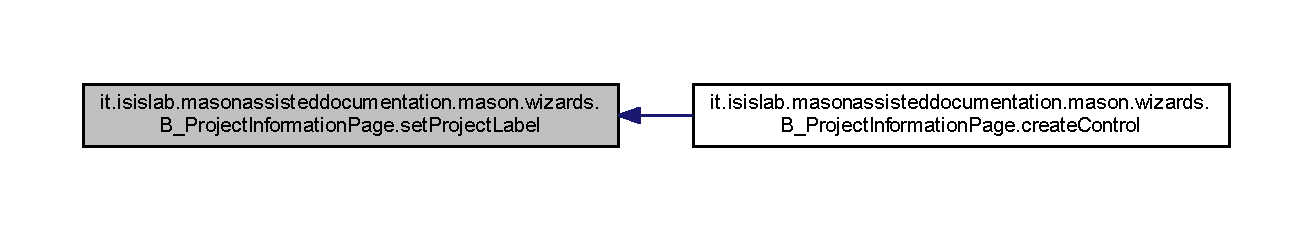
\includegraphics[width=350pt]{classit_1_1isislab_1_1masonassisteddocumentation_1_1mason_1_1wizards_1_1_b___project_information_page_af5afa21c1d0087572ad8b3d0a1a1fe9c_icgraph}
\end{center}
\end{figure}




\subsection{Member Data Documentation}
\hypertarget{classit_1_1isislab_1_1masonassisteddocumentation_1_1mason_1_1wizards_1_1_b___project_information_page_a1c3cf5ff2d1b0d408f03db81e8e40c6a}{\index{it\-::isislab\-::masonassisteddocumentation\-::mason\-::wizards\-::\-B\-\_\-\-Project\-Information\-Page@{it\-::isislab\-::masonassisteddocumentation\-::mason\-::wizards\-::\-B\-\_\-\-Project\-Information\-Page}!btn\-Auto\-Color@{btn\-Auto\-Color}}
\index{btn\-Auto\-Color@{btn\-Auto\-Color}!it::isislab::masonassisteddocumentation::mason::wizards::B_ProjectInformationPage@{it\-::isislab\-::masonassisteddocumentation\-::mason\-::wizards\-::\-B\-\_\-\-Project\-Information\-Page}}
\subsubsection[{btn\-Auto\-Color}]{\setlength{\rightskip}{0pt plus 5cm}Button it.\-isislab.\-masonassisteddocumentation.\-mason.\-wizards.\-B\-\_\-\-Project\-Information\-Page.\-btn\-Auto\-Color\hspace{0.3cm}{\ttfamily [private]}}}\label{classit_1_1isislab_1_1masonassisteddocumentation_1_1mason_1_1wizards_1_1_b___project_information_page_a1c3cf5ff2d1b0d408f03db81e8e40c6a}
\hypertarget{classit_1_1isislab_1_1masonassisteddocumentation_1_1mason_1_1wizards_1_1_b___project_information_page_a6afdf6ba02f0bf721af2acd61a2a1a5c}{\index{it\-::isislab\-::masonassisteddocumentation\-::mason\-::wizards\-::\-B\-\_\-\-Project\-Information\-Page@{it\-::isislab\-::masonassisteddocumentation\-::mason\-::wizards\-::\-B\-\_\-\-Project\-Information\-Page}!btn\-Img\-Browse@{btn\-Img\-Browse}}
\index{btn\-Img\-Browse@{btn\-Img\-Browse}!it::isislab::masonassisteddocumentation::mason::wizards::B_ProjectInformationPage@{it\-::isislab\-::masonassisteddocumentation\-::mason\-::wizards\-::\-B\-\_\-\-Project\-Information\-Page}}
\subsubsection[{btn\-Img\-Browse}]{\setlength{\rightskip}{0pt plus 5cm}Button it.\-isislab.\-masonassisteddocumentation.\-mason.\-wizards.\-B\-\_\-\-Project\-Information\-Page.\-btn\-Img\-Browse\hspace{0.3cm}{\ttfamily [private]}}}\label{classit_1_1isislab_1_1masonassisteddocumentation_1_1mason_1_1wizards_1_1_b___project_information_page_a6afdf6ba02f0bf721af2acd61a2a1a5c}
\hypertarget{classit_1_1isislab_1_1masonassisteddocumentation_1_1mason_1_1wizards_1_1_b___project_information_page_a0cbfd9890c8c62af7cfce149089682b5}{\index{it\-::isislab\-::masonassisteddocumentation\-::mason\-::wizards\-::\-B\-\_\-\-Project\-Information\-Page@{it\-::isislab\-::masonassisteddocumentation\-::mason\-::wizards\-::\-B\-\_\-\-Project\-Information\-Page}!btn\-Output\-Browse@{btn\-Output\-Browse}}
\index{btn\-Output\-Browse@{btn\-Output\-Browse}!it::isislab::masonassisteddocumentation::mason::wizards::B_ProjectInformationPage@{it\-::isislab\-::masonassisteddocumentation\-::mason\-::wizards\-::\-B\-\_\-\-Project\-Information\-Page}}
\subsubsection[{btn\-Output\-Browse}]{\setlength{\rightskip}{0pt plus 5cm}Button it.\-isislab.\-masonassisteddocumentation.\-mason.\-wizards.\-B\-\_\-\-Project\-Information\-Page.\-btn\-Output\-Browse\hspace{0.3cm}{\ttfamily [private]}}}\label{classit_1_1isislab_1_1masonassisteddocumentation_1_1mason_1_1wizards_1_1_b___project_information_page_a0cbfd9890c8c62af7cfce149089682b5}
\hypertarget{classit_1_1isislab_1_1masonassisteddocumentation_1_1mason_1_1wizards_1_1_b___project_information_page_a0c0c20817602a22ba74f88744083be6b}{\index{it\-::isislab\-::masonassisteddocumentation\-::mason\-::wizards\-::\-B\-\_\-\-Project\-Information\-Page@{it\-::isislab\-::masonassisteddocumentation\-::mason\-::wizards\-::\-B\-\_\-\-Project\-Information\-Page}!btn\-User\-Color@{btn\-User\-Color}}
\index{btn\-User\-Color@{btn\-User\-Color}!it::isislab::masonassisteddocumentation::mason::wizards::B_ProjectInformationPage@{it\-::isislab\-::masonassisteddocumentation\-::mason\-::wizards\-::\-B\-\_\-\-Project\-Information\-Page}}
\subsubsection[{btn\-User\-Color}]{\setlength{\rightskip}{0pt plus 5cm}Button it.\-isislab.\-masonassisteddocumentation.\-mason.\-wizards.\-B\-\_\-\-Project\-Information\-Page.\-btn\-User\-Color\hspace{0.3cm}{\ttfamily [private]}}}\label{classit_1_1isislab_1_1masonassisteddocumentation_1_1mason_1_1wizards_1_1_b___project_information_page_a0c0c20817602a22ba74f88744083be6b}
\hypertarget{classit_1_1isislab_1_1masonassisteddocumentation_1_1mason_1_1wizards_1_1_b___project_information_page_a0962e195aa316ea8c931a45b59971432}{\index{it\-::isislab\-::masonassisteddocumentation\-::mason\-::wizards\-::\-B\-\_\-\-Project\-Information\-Page@{it\-::isislab\-::masonassisteddocumentation\-::mason\-::wizards\-::\-B\-\_\-\-Project\-Information\-Page}!button\-Browse@{button\-Browse}}
\index{button\-Browse@{button\-Browse}!it::isislab::masonassisteddocumentation::mason::wizards::B_ProjectInformationPage@{it\-::isislab\-::masonassisteddocumentation\-::mason\-::wizards\-::\-B\-\_\-\-Project\-Information\-Page}}
\subsubsection[{button\-Browse}]{\setlength{\rightskip}{0pt plus 5cm}Button it.\-isislab.\-masonassisteddocumentation.\-mason.\-wizards.\-B\-\_\-\-Project\-Information\-Page.\-button\-Browse\hspace{0.3cm}{\ttfamily [private]}}}\label{classit_1_1isislab_1_1masonassisteddocumentation_1_1mason_1_1wizards_1_1_b___project_information_page_a0962e195aa316ea8c931a45b59971432}
\hypertarget{classit_1_1isislab_1_1masonassisteddocumentation_1_1mason_1_1wizards_1_1_b___project_information_page_ad5db74dd5c7fc084f538fde88d57573a}{\index{it\-::isislab\-::masonassisteddocumentation\-::mason\-::wizards\-::\-B\-\_\-\-Project\-Information\-Page@{it\-::isislab\-::masonassisteddocumentation\-::mason\-::wizards\-::\-B\-\_\-\-Project\-Information\-Page}!button\-Graphviz\-Browser@{button\-Graphviz\-Browser}}
\index{button\-Graphviz\-Browser@{button\-Graphviz\-Browser}!it::isislab::masonassisteddocumentation::mason::wizards::B_ProjectInformationPage@{it\-::isislab\-::masonassisteddocumentation\-::mason\-::wizards\-::\-B\-\_\-\-Project\-Information\-Page}}
\subsubsection[{button\-Graphviz\-Browser}]{\setlength{\rightskip}{0pt plus 5cm}Button it.\-isislab.\-masonassisteddocumentation.\-mason.\-wizards.\-B\-\_\-\-Project\-Information\-Page.\-button\-Graphviz\-Browser\hspace{0.3cm}{\ttfamily [private]}}}\label{classit_1_1isislab_1_1masonassisteddocumentation_1_1mason_1_1wizards_1_1_b___project_information_page_ad5db74dd5c7fc084f538fde88d57573a}
\hypertarget{classit_1_1isislab_1_1masonassisteddocumentation_1_1mason_1_1wizards_1_1_b___project_information_page_abff2b9b46293282381b6cd1b26f83792}{\index{it\-::isislab\-::masonassisteddocumentation\-::mason\-::wizards\-::\-B\-\_\-\-Project\-Information\-Page@{it\-::isislab\-::masonassisteddocumentation\-::mason\-::wizards\-::\-B\-\_\-\-Project\-Information\-Page}!composite@{composite}}
\index{composite@{composite}!it::isislab::masonassisteddocumentation::mason::wizards::B_ProjectInformationPage@{it\-::isislab\-::masonassisteddocumentation\-::mason\-::wizards\-::\-B\-\_\-\-Project\-Information\-Page}}
\subsubsection[{composite}]{\setlength{\rightskip}{0pt plus 5cm}Composite it.\-isislab.\-masonassisteddocumentation.\-mason.\-wizards.\-B\-\_\-\-Project\-Information\-Page.\-composite\hspace{0.3cm}{\ttfamily [private]}}}\label{classit_1_1isislab_1_1masonassisteddocumentation_1_1mason_1_1wizards_1_1_b___project_information_page_abff2b9b46293282381b6cd1b26f83792}
\hypertarget{classit_1_1isislab_1_1masonassisteddocumentation_1_1mason_1_1wizards_1_1_b___project_information_page_a89067957695a1743c11b64ff76f1e5c9}{\index{it\-::isislab\-::masonassisteddocumentation\-::mason\-::wizards\-::\-B\-\_\-\-Project\-Information\-Page@{it\-::isislab\-::masonassisteddocumentation\-::mason\-::wizards\-::\-B\-\_\-\-Project\-Information\-Page}!composite\-\_\-1@{composite\-\_\-1}}
\index{composite\-\_\-1@{composite\-\_\-1}!it::isislab::masonassisteddocumentation::mason::wizards::B_ProjectInformationPage@{it\-::isislab\-::masonassisteddocumentation\-::mason\-::wizards\-::\-B\-\_\-\-Project\-Information\-Page}}
\subsubsection[{composite\-\_\-1}]{\setlength{\rightskip}{0pt plus 5cm}Composite it.\-isislab.\-masonassisteddocumentation.\-mason.\-wizards.\-B\-\_\-\-Project\-Information\-Page.\-composite\-\_\-1\hspace{0.3cm}{\ttfamily [private]}}}\label{classit_1_1isislab_1_1masonassisteddocumentation_1_1mason_1_1wizards_1_1_b___project_information_page_a89067957695a1743c11b64ff76f1e5c9}
\hypertarget{classit_1_1isislab_1_1masonassisteddocumentation_1_1mason_1_1wizards_1_1_b___project_information_page_afd09135c84c569cc68148a0166b9390a}{\index{it\-::isislab\-::masonassisteddocumentation\-::mason\-::wizards\-::\-B\-\_\-\-Project\-Information\-Page@{it\-::isislab\-::masonassisteddocumentation\-::mason\-::wizards\-::\-B\-\_\-\-Project\-Information\-Page}!container\-Text@{container\-Text}}
\index{container\-Text@{container\-Text}!it::isislab::masonassisteddocumentation::mason::wizards::B_ProjectInformationPage@{it\-::isislab\-::masonassisteddocumentation\-::mason\-::wizards\-::\-B\-\_\-\-Project\-Information\-Page}}
\subsubsection[{container\-Text}]{\setlength{\rightskip}{0pt plus 5cm}Text it.\-isislab.\-masonassisteddocumentation.\-mason.\-wizards.\-B\-\_\-\-Project\-Information\-Page.\-container\-Text\hspace{0.3cm}{\ttfamily [private]}}}\label{classit_1_1isislab_1_1masonassisteddocumentation_1_1mason_1_1wizards_1_1_b___project_information_page_afd09135c84c569cc68148a0166b9390a}
\hypertarget{classit_1_1isislab_1_1masonassisteddocumentation_1_1mason_1_1wizards_1_1_b___project_information_page_a08c0494b74656d068e78bbe0a56715ed}{\index{it\-::isislab\-::masonassisteddocumentation\-::mason\-::wizards\-::\-B\-\_\-\-Project\-Information\-Page@{it\-::isislab\-::masonassisteddocumentation\-::mason\-::wizards\-::\-B\-\_\-\-Project\-Information\-Page}!label\-\_\-\-Message@{label\-\_\-\-Message}}
\index{label\-\_\-\-Message@{label\-\_\-\-Message}!it::isislab::masonassisteddocumentation::mason::wizards::B_ProjectInformationPage@{it\-::isislab\-::masonassisteddocumentation\-::mason\-::wizards\-::\-B\-\_\-\-Project\-Information\-Page}}
\subsubsection[{label\-\_\-\-Message}]{\setlength{\rightskip}{0pt plus 5cm}Label it.\-isislab.\-masonassisteddocumentation.\-mason.\-wizards.\-B\-\_\-\-Project\-Information\-Page.\-label\-\_\-\-Message\hspace{0.3cm}{\ttfamily [private]}}}\label{classit_1_1isislab_1_1masonassisteddocumentation_1_1mason_1_1wizards_1_1_b___project_information_page_a08c0494b74656d068e78bbe0a56715ed}
\hypertarget{classit_1_1isislab_1_1masonassisteddocumentation_1_1mason_1_1wizards_1_1_b___project_information_page_acb48412dbb797258e13404c757c8d3f4}{\index{it\-::isislab\-::masonassisteddocumentation\-::mason\-::wizards\-::\-B\-\_\-\-Project\-Information\-Page@{it\-::isislab\-::masonassisteddocumentation\-::mason\-::wizards\-::\-B\-\_\-\-Project\-Information\-Page}!label\-Graphviz\-Path@{label\-Graphviz\-Path}}
\index{label\-Graphviz\-Path@{label\-Graphviz\-Path}!it::isislab::masonassisteddocumentation::mason::wizards::B_ProjectInformationPage@{it\-::isislab\-::masonassisteddocumentation\-::mason\-::wizards\-::\-B\-\_\-\-Project\-Information\-Page}}
\subsubsection[{label\-Graphviz\-Path}]{\setlength{\rightskip}{0pt plus 5cm}Label it.\-isislab.\-masonassisteddocumentation.\-mason.\-wizards.\-B\-\_\-\-Project\-Information\-Page.\-label\-Graphviz\-Path\hspace{0.3cm}{\ttfamily [private]}}}\label{classit_1_1isislab_1_1masonassisteddocumentation_1_1mason_1_1wizards_1_1_b___project_information_page_acb48412dbb797258e13404c757c8d3f4}
\hypertarget{classit_1_1isislab_1_1masonassisteddocumentation_1_1mason_1_1wizards_1_1_b___project_information_page_a0cc1d0856402dfcda75702e789c68733}{\index{it\-::isislab\-::masonassisteddocumentation\-::mason\-::wizards\-::\-B\-\_\-\-Project\-Information\-Page@{it\-::isislab\-::masonassisteddocumentation\-::mason\-::wizards\-::\-B\-\_\-\-Project\-Information\-Page}!label\-User\-Color@{label\-User\-Color}}
\index{label\-User\-Color@{label\-User\-Color}!it::isislab::masonassisteddocumentation::mason::wizards::B_ProjectInformationPage@{it\-::isislab\-::masonassisteddocumentation\-::mason\-::wizards\-::\-B\-\_\-\-Project\-Information\-Page}}
\subsubsection[{label\-User\-Color}]{\setlength{\rightskip}{0pt plus 5cm}Label it.\-isislab.\-masonassisteddocumentation.\-mason.\-wizards.\-B\-\_\-\-Project\-Information\-Page.\-label\-User\-Color\hspace{0.3cm}{\ttfamily [private]}}}\label{classit_1_1isislab_1_1masonassisteddocumentation_1_1mason_1_1wizards_1_1_b___project_information_page_a0cc1d0856402dfcda75702e789c68733}
\hypertarget{classit_1_1isislab_1_1masonassisteddocumentation_1_1mason_1_1wizards_1_1_b___project_information_page_af5b4ee969085257cfe8a66867d217b8d}{\index{it\-::isislab\-::masonassisteddocumentation\-::mason\-::wizards\-::\-B\-\_\-\-Project\-Information\-Page@{it\-::isislab\-::masonassisteddocumentation\-::mason\-::wizards\-::\-B\-\_\-\-Project\-Information\-Page}!lbl\-Agent@{lbl\-Agent}}
\index{lbl\-Agent@{lbl\-Agent}!it::isislab::masonassisteddocumentation::mason::wizards::B_ProjectInformationPage@{it\-::isislab\-::masonassisteddocumentation\-::mason\-::wizards\-::\-B\-\_\-\-Project\-Information\-Page}}
\subsubsection[{lbl\-Agent}]{\setlength{\rightskip}{0pt plus 5cm}Label it.\-isislab.\-masonassisteddocumentation.\-mason.\-wizards.\-B\-\_\-\-Project\-Information\-Page.\-lbl\-Agent\hspace{0.3cm}{\ttfamily [private]}}}\label{classit_1_1isislab_1_1masonassisteddocumentation_1_1mason_1_1wizards_1_1_b___project_information_page_af5b4ee969085257cfe8a66867d217b8d}
\hypertarget{classit_1_1isislab_1_1masonassisteddocumentation_1_1mason_1_1wizards_1_1_b___project_information_page_a9c18ade9b232612291e8a831823a29cf}{\index{it\-::isislab\-::masonassisteddocumentation\-::mason\-::wizards\-::\-B\-\_\-\-Project\-Information\-Page@{it\-::isislab\-::masonassisteddocumentation\-::mason\-::wizards\-::\-B\-\_\-\-Project\-Information\-Page}!lbl\-Auto\-Color@{lbl\-Auto\-Color}}
\index{lbl\-Auto\-Color@{lbl\-Auto\-Color}!it::isislab::masonassisteddocumentation::mason::wizards::B_ProjectInformationPage@{it\-::isislab\-::masonassisteddocumentation\-::mason\-::wizards\-::\-B\-\_\-\-Project\-Information\-Page}}
\subsubsection[{lbl\-Auto\-Color}]{\setlength{\rightskip}{0pt plus 5cm}Label it.\-isislab.\-masonassisteddocumentation.\-mason.\-wizards.\-B\-\_\-\-Project\-Information\-Page.\-lbl\-Auto\-Color\hspace{0.3cm}{\ttfamily [private]}}}\label{classit_1_1isislab_1_1masonassisteddocumentation_1_1mason_1_1wizards_1_1_b___project_information_page_a9c18ade9b232612291e8a831823a29cf}
\hypertarget{classit_1_1isislab_1_1masonassisteddocumentation_1_1mason_1_1wizards_1_1_b___project_information_page_a4887707c3be26291594a2d0010abd500}{\index{it\-::isislab\-::masonassisteddocumentation\-::mason\-::wizards\-::\-B\-\_\-\-Project\-Information\-Page@{it\-::isislab\-::masonassisteddocumentation\-::mason\-::wizards\-::\-B\-\_\-\-Project\-Information\-Page}!lbl\-Doxygen\-Path@{lbl\-Doxygen\-Path}}
\index{lbl\-Doxygen\-Path@{lbl\-Doxygen\-Path}!it::isislab::masonassisteddocumentation::mason::wizards::B_ProjectInformationPage@{it\-::isislab\-::masonassisteddocumentation\-::mason\-::wizards\-::\-B\-\_\-\-Project\-Information\-Page}}
\subsubsection[{lbl\-Doxygen\-Path}]{\setlength{\rightskip}{0pt plus 5cm}Label it.\-isislab.\-masonassisteddocumentation.\-mason.\-wizards.\-B\-\_\-\-Project\-Information\-Page.\-lbl\-Doxygen\-Path\hspace{0.3cm}{\ttfamily [private]}}}\label{classit_1_1isislab_1_1masonassisteddocumentation_1_1mason_1_1wizards_1_1_b___project_information_page_a4887707c3be26291594a2d0010abd500}
\hypertarget{classit_1_1isislab_1_1masonassisteddocumentation_1_1mason_1_1wizards_1_1_b___project_information_page_a65bb7c12ddee14a56433fb0af2e97e89}{\index{it\-::isislab\-::masonassisteddocumentation\-::mason\-::wizards\-::\-B\-\_\-\-Project\-Information\-Page@{it\-::isislab\-::masonassisteddocumentation\-::mason\-::wizards\-::\-B\-\_\-\-Project\-Information\-Page}!lbl\-Gui\-State@{lbl\-Gui\-State}}
\index{lbl\-Gui\-State@{lbl\-Gui\-State}!it::isislab::masonassisteddocumentation::mason::wizards::B_ProjectInformationPage@{it\-::isislab\-::masonassisteddocumentation\-::mason\-::wizards\-::\-B\-\_\-\-Project\-Information\-Page}}
\subsubsection[{lbl\-Gui\-State}]{\setlength{\rightskip}{0pt plus 5cm}Label it.\-isislab.\-masonassisteddocumentation.\-mason.\-wizards.\-B\-\_\-\-Project\-Information\-Page.\-lbl\-Gui\-State\hspace{0.3cm}{\ttfamily [private]}}}\label{classit_1_1isislab_1_1masonassisteddocumentation_1_1mason_1_1wizards_1_1_b___project_information_page_a65bb7c12ddee14a56433fb0af2e97e89}
\hypertarget{classit_1_1isislab_1_1masonassisteddocumentation_1_1mason_1_1wizards_1_1_b___project_information_page_a6c9ce7d939e8bd032a1f2fb5e42f0d78}{\index{it\-::isislab\-::masonassisteddocumentation\-::mason\-::wizards\-::\-B\-\_\-\-Project\-Information\-Page@{it\-::isislab\-::masonassisteddocumentation\-::mason\-::wizards\-::\-B\-\_\-\-Project\-Information\-Page}!lbl\-Image\-Path@{lbl\-Image\-Path}}
\index{lbl\-Image\-Path@{lbl\-Image\-Path}!it::isislab::masonassisteddocumentation::mason::wizards::B_ProjectInformationPage@{it\-::isislab\-::masonassisteddocumentation\-::mason\-::wizards\-::\-B\-\_\-\-Project\-Information\-Page}}
\subsubsection[{lbl\-Image\-Path}]{\setlength{\rightskip}{0pt plus 5cm}Label it.\-isislab.\-masonassisteddocumentation.\-mason.\-wizards.\-B\-\_\-\-Project\-Information\-Page.\-lbl\-Image\-Path\hspace{0.3cm}{\ttfamily [private]}}}\label{classit_1_1isislab_1_1masonassisteddocumentation_1_1mason_1_1wizards_1_1_b___project_information_page_a6c9ce7d939e8bd032a1f2fb5e42f0d78}
\hypertarget{classit_1_1isislab_1_1masonassisteddocumentation_1_1mason_1_1wizards_1_1_b___project_information_page_a801e6444bc2096376ffbfd62f2660aaf}{\index{it\-::isislab\-::masonassisteddocumentation\-::mason\-::wizards\-::\-B\-\_\-\-Project\-Information\-Page@{it\-::isislab\-::masonassisteddocumentation\-::mason\-::wizards\-::\-B\-\_\-\-Project\-Information\-Page}!lbl\-Project\-Found@{lbl\-Project\-Found}}
\index{lbl\-Project\-Found@{lbl\-Project\-Found}!it::isislab::masonassisteddocumentation::mason::wizards::B_ProjectInformationPage@{it\-::isislab\-::masonassisteddocumentation\-::mason\-::wizards\-::\-B\-\_\-\-Project\-Information\-Page}}
\subsubsection[{lbl\-Project\-Found}]{\setlength{\rightskip}{0pt plus 5cm}Label it.\-isislab.\-masonassisteddocumentation.\-mason.\-wizards.\-B\-\_\-\-Project\-Information\-Page.\-lbl\-Project\-Found\hspace{0.3cm}{\ttfamily [private]}}}\label{classit_1_1isislab_1_1masonassisteddocumentation_1_1mason_1_1wizards_1_1_b___project_information_page_a801e6444bc2096376ffbfd62f2660aaf}
\hypertarget{classit_1_1isislab_1_1masonassisteddocumentation_1_1mason_1_1wizards_1_1_b___project_information_page_aa7b41a14af9155e5feaff4060af3a2c4}{\index{it\-::isislab\-::masonassisteddocumentation\-::mason\-::wizards\-::\-B\-\_\-\-Project\-Information\-Page@{it\-::isislab\-::masonassisteddocumentation\-::mason\-::wizards\-::\-B\-\_\-\-Project\-Information\-Page}!lbl\-Sim\-State@{lbl\-Sim\-State}}
\index{lbl\-Sim\-State@{lbl\-Sim\-State}!it::isislab::masonassisteddocumentation::mason::wizards::B_ProjectInformationPage@{it\-::isislab\-::masonassisteddocumentation\-::mason\-::wizards\-::\-B\-\_\-\-Project\-Information\-Page}}
\subsubsection[{lbl\-Sim\-State}]{\setlength{\rightskip}{0pt plus 5cm}Label it.\-isislab.\-masonassisteddocumentation.\-mason.\-wizards.\-B\-\_\-\-Project\-Information\-Page.\-lbl\-Sim\-State\hspace{0.3cm}{\ttfamily [private]}}}\label{classit_1_1isislab_1_1masonassisteddocumentation_1_1mason_1_1wizards_1_1_b___project_information_page_aa7b41a14af9155e5feaff4060af3a2c4}
\hypertarget{classit_1_1isislab_1_1masonassisteddocumentation_1_1mason_1_1wizards_1_1_b___project_information_page_ae3ce9b9ca6502f09db614860f5a1a127}{\index{it\-::isislab\-::masonassisteddocumentation\-::mason\-::wizards\-::\-B\-\_\-\-Project\-Information\-Page@{it\-::isislab\-::masonassisteddocumentation\-::mason\-::wizards\-::\-B\-\_\-\-Project\-Information\-Page}!lbl\-View\-Auto\-Color@{lbl\-View\-Auto\-Color}}
\index{lbl\-View\-Auto\-Color@{lbl\-View\-Auto\-Color}!it::isislab::masonassisteddocumentation::mason::wizards::B_ProjectInformationPage@{it\-::isislab\-::masonassisteddocumentation\-::mason\-::wizards\-::\-B\-\_\-\-Project\-Information\-Page}}
\subsubsection[{lbl\-View\-Auto\-Color}]{\setlength{\rightskip}{0pt plus 5cm}Label it.\-isislab.\-masonassisteddocumentation.\-mason.\-wizards.\-B\-\_\-\-Project\-Information\-Page.\-lbl\-View\-Auto\-Color\hspace{0.3cm}{\ttfamily [private]}}}\label{classit_1_1isislab_1_1masonassisteddocumentation_1_1mason_1_1wizards_1_1_b___project_information_page_ae3ce9b9ca6502f09db614860f5a1a127}
\hypertarget{classit_1_1isislab_1_1masonassisteddocumentation_1_1mason_1_1wizards_1_1_b___project_information_page_abf3d5350bf4a246805afb445ef49380a}{\index{it\-::isislab\-::masonassisteddocumentation\-::mason\-::wizards\-::\-B\-\_\-\-Project\-Information\-Page@{it\-::isislab\-::masonassisteddocumentation\-::mason\-::wizards\-::\-B\-\_\-\-Project\-Information\-Page}!lbl\-View\-User\-Color@{lbl\-View\-User\-Color}}
\index{lbl\-View\-User\-Color@{lbl\-View\-User\-Color}!it::isislab::masonassisteddocumentation::mason::wizards::B_ProjectInformationPage@{it\-::isislab\-::masonassisteddocumentation\-::mason\-::wizards\-::\-B\-\_\-\-Project\-Information\-Page}}
\subsubsection[{lbl\-View\-User\-Color}]{\setlength{\rightskip}{0pt plus 5cm}Label it.\-isislab.\-masonassisteddocumentation.\-mason.\-wizards.\-B\-\_\-\-Project\-Information\-Page.\-lbl\-View\-User\-Color\hspace{0.3cm}{\ttfamily [private]}}}\label{classit_1_1isislab_1_1masonassisteddocumentation_1_1mason_1_1wizards_1_1_b___project_information_page_abf3d5350bf4a246805afb445ef49380a}
\hypertarget{classit_1_1isislab_1_1masonassisteddocumentation_1_1mason_1_1wizards_1_1_b___project_information_page_a0950f901b19ba8f8e20acdd4d69fd720}{\index{it\-::isislab\-::masonassisteddocumentation\-::mason\-::wizards\-::\-B\-\_\-\-Project\-Information\-Page@{it\-::isislab\-::masonassisteddocumentation\-::mason\-::wizards\-::\-B\-\_\-\-Project\-Information\-Page}!log@{log}}
\index{log@{log}!it::isislab::masonassisteddocumentation::mason::wizards::B_ProjectInformationPage@{it\-::isislab\-::masonassisteddocumentation\-::mason\-::wizards\-::\-B\-\_\-\-Project\-Information\-Page}}
\subsubsection[{log}]{\setlength{\rightskip}{0pt plus 5cm}Logger it.\-isislab.\-masonassisteddocumentation.\-mason.\-wizards.\-B\-\_\-\-Project\-Information\-Page.\-log = Logger.\-get\-Logger(\char`\"{}global\char`\"{})\hspace{0.3cm}{\ttfamily [static]}, {\ttfamily [private]}}}\label{classit_1_1isislab_1_1masonassisteddocumentation_1_1mason_1_1wizards_1_1_b___project_information_page_a0950f901b19ba8f8e20acdd4d69fd720}
\hypertarget{classit_1_1isislab_1_1masonassisteddocumentation_1_1mason_1_1wizards_1_1_b___project_information_page_a5129feb0fa34a1d51e44a2fe495ac42c}{\index{it\-::isislab\-::masonassisteddocumentation\-::mason\-::wizards\-::\-B\-\_\-\-Project\-Information\-Page@{it\-::isislab\-::masonassisteddocumentation\-::mason\-::wizards\-::\-B\-\_\-\-Project\-Information\-Page}!project\-Analizer@{project\-Analizer}}
\index{project\-Analizer@{project\-Analizer}!it::isislab::masonassisteddocumentation::mason::wizards::B_ProjectInformationPage@{it\-::isislab\-::masonassisteddocumentation\-::mason\-::wizards\-::\-B\-\_\-\-Project\-Information\-Page}}
\subsubsection[{project\-Analizer}]{\setlength{\rightskip}{0pt plus 5cm}{\bf Project\-Analizer} it.\-isislab.\-masonassisteddocumentation.\-mason.\-wizards.\-B\-\_\-\-Project\-Information\-Page.\-project\-Analizer\hspace{0.3cm}{\ttfamily [private]}}}\label{classit_1_1isislab_1_1masonassisteddocumentation_1_1mason_1_1wizards_1_1_b___project_information_page_a5129feb0fa34a1d51e44a2fe495ac42c}
\hypertarget{classit_1_1isislab_1_1masonassisteddocumentation_1_1mason_1_1wizards_1_1_b___project_information_page_adf33db8f408e4f486a256d199eae3bae}{\index{it\-::isislab\-::masonassisteddocumentation\-::mason\-::wizards\-::\-B\-\_\-\-Project\-Information\-Page@{it\-::isislab\-::masonassisteddocumentation\-::mason\-::wizards\-::\-B\-\_\-\-Project\-Information\-Page}!scrolled\-Composite@{scrolled\-Composite}}
\index{scrolled\-Composite@{scrolled\-Composite}!it::isislab::masonassisteddocumentation::mason::wizards::B_ProjectInformationPage@{it\-::isislab\-::masonassisteddocumentation\-::mason\-::wizards\-::\-B\-\_\-\-Project\-Information\-Page}}
\subsubsection[{scrolled\-Composite}]{\setlength{\rightskip}{0pt plus 5cm}Scrolled\-Composite it.\-isislab.\-masonassisteddocumentation.\-mason.\-wizards.\-B\-\_\-\-Project\-Information\-Page.\-scrolled\-Composite\hspace{0.3cm}{\ttfamily [private]}}}\label{classit_1_1isislab_1_1masonassisteddocumentation_1_1mason_1_1wizards_1_1_b___project_information_page_adf33db8f408e4f486a256d199eae3bae}
\hypertarget{classit_1_1isislab_1_1masonassisteddocumentation_1_1mason_1_1wizards_1_1_b___project_information_page_aae0eab045b1d0530a794116410ae6e5d}{\index{it\-::isislab\-::masonassisteddocumentation\-::mason\-::wizards\-::\-B\-\_\-\-Project\-Information\-Page@{it\-::isislab\-::masonassisteddocumentation\-::mason\-::wizards\-::\-B\-\_\-\-Project\-Information\-Page}!text@{text}}
\index{text@{text}!it::isislab::masonassisteddocumentation::mason::wizards::B_ProjectInformationPage@{it\-::isislab\-::masonassisteddocumentation\-::mason\-::wizards\-::\-B\-\_\-\-Project\-Information\-Page}}
\subsubsection[{text}]{\setlength{\rightskip}{0pt plus 5cm}Text it.\-isislab.\-masonassisteddocumentation.\-mason.\-wizards.\-B\-\_\-\-Project\-Information\-Page.\-text\hspace{0.3cm}{\ttfamily [private]}}}\label{classit_1_1isislab_1_1masonassisteddocumentation_1_1mason_1_1wizards_1_1_b___project_information_page_aae0eab045b1d0530a794116410ae6e5d}
\hypertarget{classit_1_1isislab_1_1masonassisteddocumentation_1_1mason_1_1wizards_1_1_b___project_information_page_a03d43e1fbcdb5d7d5e6745d8f57db84b}{\index{it\-::isislab\-::masonassisteddocumentation\-::mason\-::wizards\-::\-B\-\_\-\-Project\-Information\-Page@{it\-::isislab\-::masonassisteddocumentation\-::mason\-::wizards\-::\-B\-\_\-\-Project\-Information\-Page}!text\-Graphviz\-Path@{text\-Graphviz\-Path}}
\index{text\-Graphviz\-Path@{text\-Graphviz\-Path}!it::isislab::masonassisteddocumentation::mason::wizards::B_ProjectInformationPage@{it\-::isislab\-::masonassisteddocumentation\-::mason\-::wizards\-::\-B\-\_\-\-Project\-Information\-Page}}
\subsubsection[{text\-Graphviz\-Path}]{\setlength{\rightskip}{0pt plus 5cm}Text it.\-isislab.\-masonassisteddocumentation.\-mason.\-wizards.\-B\-\_\-\-Project\-Information\-Page.\-text\-Graphviz\-Path\hspace{0.3cm}{\ttfamily [private]}}}\label{classit_1_1isislab_1_1masonassisteddocumentation_1_1mason_1_1wizards_1_1_b___project_information_page_a03d43e1fbcdb5d7d5e6745d8f57db84b}
\hypertarget{classit_1_1isislab_1_1masonassisteddocumentation_1_1mason_1_1wizards_1_1_b___project_information_page_a1217897a98e0714c9e7d8141b4e931d1}{\index{it\-::isislab\-::masonassisteddocumentation\-::mason\-::wizards\-::\-B\-\_\-\-Project\-Information\-Page@{it\-::isislab\-::masonassisteddocumentation\-::mason\-::wizards\-::\-B\-\_\-\-Project\-Information\-Page}!text\-Img\-Path@{text\-Img\-Path}}
\index{text\-Img\-Path@{text\-Img\-Path}!it::isislab::masonassisteddocumentation::mason::wizards::B_ProjectInformationPage@{it\-::isislab\-::masonassisteddocumentation\-::mason\-::wizards\-::\-B\-\_\-\-Project\-Information\-Page}}
\subsubsection[{text\-Img\-Path}]{\setlength{\rightskip}{0pt plus 5cm}Text it.\-isislab.\-masonassisteddocumentation.\-mason.\-wizards.\-B\-\_\-\-Project\-Information\-Page.\-text\-Img\-Path\hspace{0.3cm}{\ttfamily [private]}}}\label{classit_1_1isislab_1_1masonassisteddocumentation_1_1mason_1_1wizards_1_1_b___project_information_page_a1217897a98e0714c9e7d8141b4e931d1}


The documentation for this class was generated from the following file\-:\begin{DoxyCompactItemize}
\item 
src/it/isislab/masonassisteddocumentation/mason/wizards/\hyperlink{_b___project_information_page_8java}{B\-\_\-\-Project\-Information\-Page.\-java}\end{DoxyCompactItemize}

\hypertarget{classit_1_1isislab_1_1masonassisteddocumentation_1_1mason_1_1wizards_1_1_c___purpose_page}{\section{it.\-isislab.\-masonassisteddocumentation.\-mason.\-wizards.\-C\-\_\-\-Purpose\-Page Class Reference}
\label{classit_1_1isislab_1_1masonassisteddocumentation_1_1mason_1_1wizards_1_1_c___purpose_page}\index{it.\-isislab.\-masonassisteddocumentation.\-mason.\-wizards.\-C\-\_\-\-Purpose\-Page@{it.\-isislab.\-masonassisteddocumentation.\-mason.\-wizards.\-C\-\_\-\-Purpose\-Page}}
}


Inheritance diagram for it.\-isislab.\-masonassisteddocumentation.\-mason.\-wizards.\-C\-\_\-\-Purpose\-Page\-:
\nopagebreak
\begin{figure}[H]
\begin{center}
\leavevmode
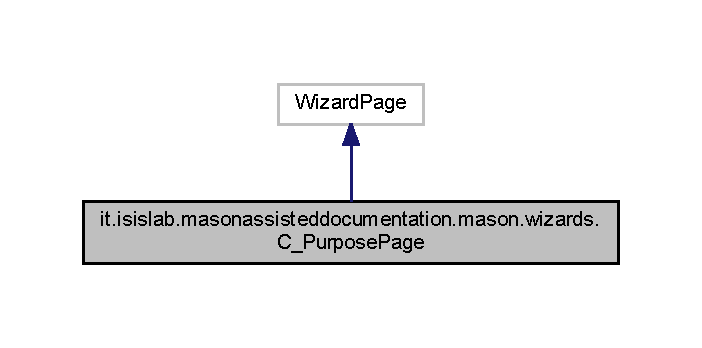
\includegraphics[width=337pt]{classit_1_1isislab_1_1masonassisteddocumentation_1_1mason_1_1wizards_1_1_c___purpose_page__inherit__graph}
\end{center}
\end{figure}


Collaboration diagram for it.\-isislab.\-masonassisteddocumentation.\-mason.\-wizards.\-C\-\_\-\-Purpose\-Page\-:
\nopagebreak
\begin{figure}[H]
\begin{center}
\leavevmode
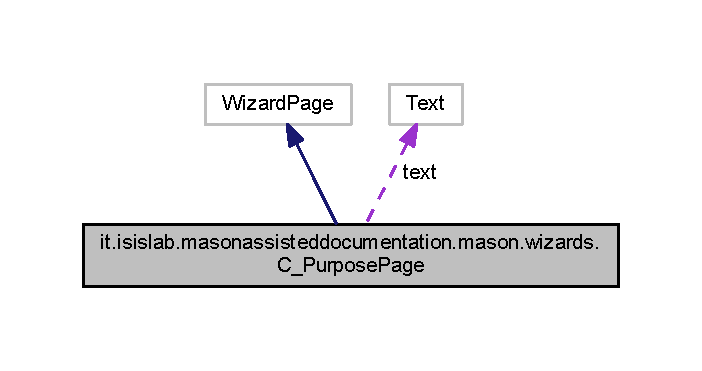
\includegraphics[width=337pt]{classit_1_1isislab_1_1masonassisteddocumentation_1_1mason_1_1wizards_1_1_c___purpose_page__coll__graph}
\end{center}
\end{figure}
\subsection*{Public Member Functions}
\begin{DoxyCompactItemize}
\item 
\hyperlink{classit_1_1isislab_1_1masonassisteddocumentation_1_1mason_1_1wizards_1_1_c___purpose_page_a5cc12f672a96e503aa641ddf061335c4}{C\-\_\-\-Purpose\-Page} ()
\item 
void \hyperlink{classit_1_1isislab_1_1masonassisteddocumentation_1_1mason_1_1wizards_1_1_c___purpose_page_ab9d7e8c0b517bbbb5c1d1ae4c11d13b7}{create\-Control} (Composite parent)
\item 
I\-Wizard\-Page \hyperlink{classit_1_1isislab_1_1masonassisteddocumentation_1_1mason_1_1wizards_1_1_c___purpose_page_a4ed9bb021ee9454f16449dda33c492de}{get\-Next\-Page} ()
\end{DoxyCompactItemize}
\subsection*{Private Member Functions}
\begin{DoxyCompactItemize}
\item 
void \hyperlink{classit_1_1isislab_1_1masonassisteddocumentation_1_1mason_1_1wizards_1_1_c___purpose_page_a6c01f630e4fd58c3f5640da22772bbc4}{get\-Old\-Information} ()
\end{DoxyCompactItemize}
\subsection*{Private Attributes}
\begin{DoxyCompactItemize}
\item 
Text \hyperlink{classit_1_1isislab_1_1masonassisteddocumentation_1_1mason_1_1wizards_1_1_c___purpose_page_ac7b1a3918766a267a7594f729ea7faac}{text}
\end{DoxyCompactItemize}
\subsection*{Static Private Attributes}
\begin{DoxyCompactItemize}
\item 
static String \hyperlink{classit_1_1isislab_1_1masonassisteddocumentation_1_1mason_1_1wizards_1_1_c___purpose_page_a62e6e8e416e6c87fd490db86b8085533}{page\-Description} = \char`\"{}What is the purpose of the model?\char`\"{}
\end{DoxyCompactItemize}


\subsection{Constructor \& Destructor Documentation}
\hypertarget{classit_1_1isislab_1_1masonassisteddocumentation_1_1mason_1_1wizards_1_1_c___purpose_page_a5cc12f672a96e503aa641ddf061335c4}{\index{it\-::isislab\-::masonassisteddocumentation\-::mason\-::wizards\-::\-C\-\_\-\-Purpose\-Page@{it\-::isislab\-::masonassisteddocumentation\-::mason\-::wizards\-::\-C\-\_\-\-Purpose\-Page}!C\-\_\-\-Purpose\-Page@{C\-\_\-\-Purpose\-Page}}
\index{C\-\_\-\-Purpose\-Page@{C\-\_\-\-Purpose\-Page}!it::isislab::masonassisteddocumentation::mason::wizards::C_PurposePage@{it\-::isislab\-::masonassisteddocumentation\-::mason\-::wizards\-::\-C\-\_\-\-Purpose\-Page}}
\subsubsection[{C\-\_\-\-Purpose\-Page}]{\setlength{\rightskip}{0pt plus 5cm}it.\-isislab.\-masonassisteddocumentation.\-mason.\-wizards.\-C\-\_\-\-Purpose\-Page.\-C\-\_\-\-Purpose\-Page (
\begin{DoxyParamCaption}
{}
\end{DoxyParamCaption}
)}}\label{classit_1_1isislab_1_1masonassisteddocumentation_1_1mason_1_1wizards_1_1_c___purpose_page_a5cc12f672a96e503aa641ddf061335c4}

\begin{DoxyCode}
18                            \{
19         super(\textcolor{stringliteral}{"wizardPage"});
20         setTitle(\textcolor{stringliteral}{"1/7 - Purpose"});
21         setDescription(\hyperlink{classit_1_1isislab_1_1masonassisteddocumentation_1_1mason_1_1wizards_1_1_c___purpose_page_a62e6e8e416e6c87fd490db86b8085533}{pageDescription});
22     \}
\end{DoxyCode}


\subsection{Member Function Documentation}
\hypertarget{classit_1_1isislab_1_1masonassisteddocumentation_1_1mason_1_1wizards_1_1_c___purpose_page_ab9d7e8c0b517bbbb5c1d1ae4c11d13b7}{\index{it\-::isislab\-::masonassisteddocumentation\-::mason\-::wizards\-::\-C\-\_\-\-Purpose\-Page@{it\-::isislab\-::masonassisteddocumentation\-::mason\-::wizards\-::\-C\-\_\-\-Purpose\-Page}!create\-Control@{create\-Control}}
\index{create\-Control@{create\-Control}!it::isislab::masonassisteddocumentation::mason::wizards::C_PurposePage@{it\-::isislab\-::masonassisteddocumentation\-::mason\-::wizards\-::\-C\-\_\-\-Purpose\-Page}}
\subsubsection[{create\-Control}]{\setlength{\rightskip}{0pt plus 5cm}void it.\-isislab.\-masonassisteddocumentation.\-mason.\-wizards.\-C\-\_\-\-Purpose\-Page.\-create\-Control (
\begin{DoxyParamCaption}
\item[{Composite}]{parent}
\end{DoxyParamCaption}
)}}\label{classit_1_1isislab_1_1masonassisteddocumentation_1_1mason_1_1wizards_1_1_c___purpose_page_ab9d7e8c0b517bbbb5c1d1ae4c11d13b7}

\begin{DoxyCode}
24                                                 \{
25         Composite container = \textcolor{keyword}{new} Composite(parent, SWT.NULL);
26         setControl(container);
27         container.setLayout(\textcolor{keyword}{new} GridLayout(1, \textcolor{keyword}{false}));      
28         
29         ScrolledComposite scrolledComposite = \textcolor{keyword}{new} ScrolledComposite(container, SWT.BORDER | SWT.H\_SCROLL | 
      SWT.V\_SCROLL);
30         scrolledComposite.setExpandHorizontal(\textcolor{keyword}{true});
31         scrolledComposite.setExpandVertical(\textcolor{keyword}{true});
32         
33         Composite composite = \textcolor{keyword}{new} Composite(scrolledComposite, SWT.NONE);
34         \hyperlink{classit_1_1isislab_1_1masonassisteddocumentation_1_1mason_1_1wizards_1_1_c___purpose_page_ac7b1a3918766a267a7594f729ea7faac}{text} = \textcolor{keyword}{new} Text(composite, SWT.BORDER | SWT.H\_SCROLL | SWT.V\_SCROLL | SWT.CANCEL | SWT.MULTI);
35         text.setLocation(0, 0);
36         text.setSize(562, 269);
37         scrolledComposite.setContent(composite);
38         scrolledComposite.setMinSize(composite.computeSize(SWT.DEFAULT, SWT.DEFAULT));
39         \hyperlink{classit_1_1isislab_1_1masonassisteddocumentation_1_1mason_1_1wizards_1_1_c___purpose_page_a6c01f630e4fd58c3f5640da22772bbc4}{getOldInformation}();
40     \}
\end{DoxyCode}


Here is the call graph for this function\-:
\nopagebreak
\begin{figure}[H]
\begin{center}
\leavevmode
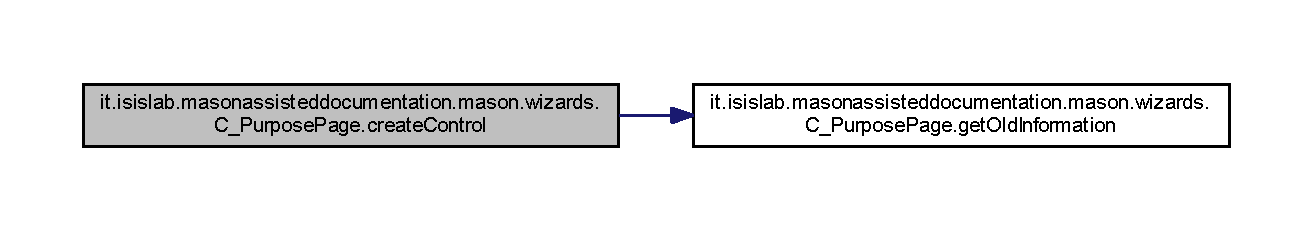
\includegraphics[width=350pt]{classit_1_1isislab_1_1masonassisteddocumentation_1_1mason_1_1wizards_1_1_c___purpose_page_ab9d7e8c0b517bbbb5c1d1ae4c11d13b7_cgraph}
\end{center}
\end{figure}


\hypertarget{classit_1_1isislab_1_1masonassisteddocumentation_1_1mason_1_1wizards_1_1_c___purpose_page_a4ed9bb021ee9454f16449dda33c492de}{\index{it\-::isislab\-::masonassisteddocumentation\-::mason\-::wizards\-::\-C\-\_\-\-Purpose\-Page@{it\-::isislab\-::masonassisteddocumentation\-::mason\-::wizards\-::\-C\-\_\-\-Purpose\-Page}!get\-Next\-Page@{get\-Next\-Page}}
\index{get\-Next\-Page@{get\-Next\-Page}!it::isislab::masonassisteddocumentation::mason::wizards::C_PurposePage@{it\-::isislab\-::masonassisteddocumentation\-::mason\-::wizards\-::\-C\-\_\-\-Purpose\-Page}}
\subsubsection[{get\-Next\-Page}]{\setlength{\rightskip}{0pt plus 5cm}I\-Wizard\-Page it.\-isislab.\-masonassisteddocumentation.\-mason.\-wizards.\-C\-\_\-\-Purpose\-Page.\-get\-Next\-Page (
\begin{DoxyParamCaption}
{}
\end{DoxyParamCaption}
)}}\label{classit_1_1isislab_1_1masonassisteddocumentation_1_1mason_1_1wizards_1_1_c___purpose_page_a4ed9bb021ee9454f16449dda33c492de}

\begin{DoxyCode}
49                                     \{ 
50         \textcolor{comment}{//******store information******//}
51         ODD.getPurpose().setModelPurpose(\hyperlink{classit_1_1isislab_1_1masonassisteddocumentation_1_1mason_1_1wizards_1_1_c___purpose_page_ac7b1a3918766a267a7594f729ea7faac}{text}.getText());
52         \textcolor{comment}{//****selecting right page****//}
53         \textcolor{keywordflow}{if} (GlobalUtility.getAgentAnalizer() != null)\{
54             D\_AgentDescriptionPage nextPage = \textcolor{keyword}{new} D\_AgentDescriptionPage();
55             ((MASONDocumentationWizard) super.getWizard()).addPage(nextPage);
56             \textcolor{keywordflow}{return} nextPage;
57         \}
58         \textcolor{keywordflow}{else}\{
59             G\_GridsCellPage nextPage = \textcolor{keyword}{new} G\_GridsCellPage();
60             ((MASONDocumentationWizard) super.getWizard()).addPage(nextPage);
61             \textcolor{keywordflow}{return} nextPage;
62         \}
63     \}
\end{DoxyCode}


Here is the call graph for this function\-:
\nopagebreak
\begin{figure}[H]
\begin{center}
\leavevmode
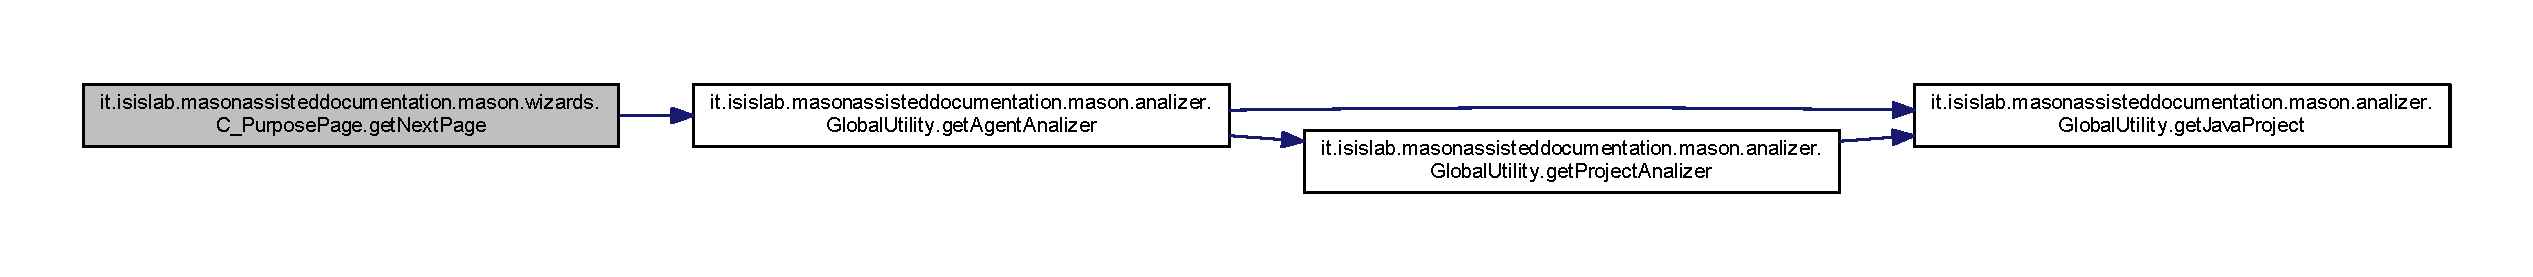
\includegraphics[width=350pt]{classit_1_1isislab_1_1masonassisteddocumentation_1_1mason_1_1wizards_1_1_c___purpose_page_a4ed9bb021ee9454f16449dda33c492de_cgraph}
\end{center}
\end{figure}


\hypertarget{classit_1_1isislab_1_1masonassisteddocumentation_1_1mason_1_1wizards_1_1_c___purpose_page_a6c01f630e4fd58c3f5640da22772bbc4}{\index{it\-::isislab\-::masonassisteddocumentation\-::mason\-::wizards\-::\-C\-\_\-\-Purpose\-Page@{it\-::isislab\-::masonassisteddocumentation\-::mason\-::wizards\-::\-C\-\_\-\-Purpose\-Page}!get\-Old\-Information@{get\-Old\-Information}}
\index{get\-Old\-Information@{get\-Old\-Information}!it::isislab::masonassisteddocumentation::mason::wizards::C_PurposePage@{it\-::isislab\-::masonassisteddocumentation\-::mason\-::wizards\-::\-C\-\_\-\-Purpose\-Page}}
\subsubsection[{get\-Old\-Information}]{\setlength{\rightskip}{0pt plus 5cm}void it.\-isislab.\-masonassisteddocumentation.\-mason.\-wizards.\-C\-\_\-\-Purpose\-Page.\-get\-Old\-Information (
\begin{DoxyParamCaption}
{}
\end{DoxyParamCaption}
)\hspace{0.3cm}{\ttfamily [private]}}}\label{classit_1_1isislab_1_1masonassisteddocumentation_1_1mason_1_1wizards_1_1_c___purpose_page_a6c01f630e4fd58c3f5640da22772bbc4}
This method get old model description (if exist). 
\begin{DoxyCode}
45                                      \{
46         text.setText(ODD.getPurpose().getModelPurpose());
47     \}
\end{DoxyCode}


Here is the caller graph for this function\-:
\nopagebreak
\begin{figure}[H]
\begin{center}
\leavevmode
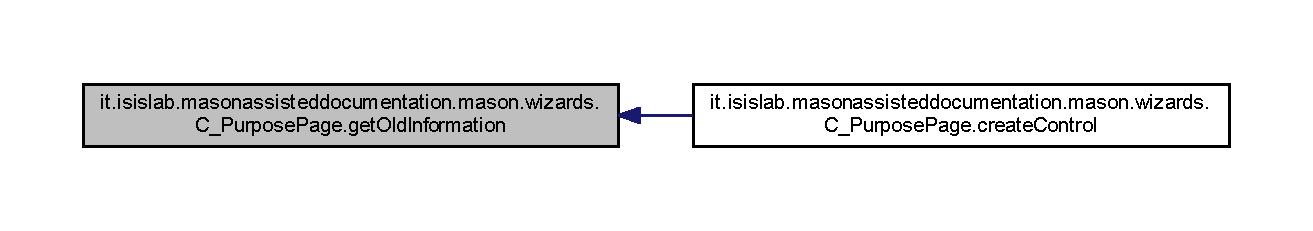
\includegraphics[width=350pt]{classit_1_1isislab_1_1masonassisteddocumentation_1_1mason_1_1wizards_1_1_c___purpose_page_a6c01f630e4fd58c3f5640da22772bbc4_icgraph}
\end{center}
\end{figure}




\subsection{Member Data Documentation}
\hypertarget{classit_1_1isislab_1_1masonassisteddocumentation_1_1mason_1_1wizards_1_1_c___purpose_page_a62e6e8e416e6c87fd490db86b8085533}{\index{it\-::isislab\-::masonassisteddocumentation\-::mason\-::wizards\-::\-C\-\_\-\-Purpose\-Page@{it\-::isislab\-::masonassisteddocumentation\-::mason\-::wizards\-::\-C\-\_\-\-Purpose\-Page}!page\-Description@{page\-Description}}
\index{page\-Description@{page\-Description}!it::isislab::masonassisteddocumentation::mason::wizards::C_PurposePage@{it\-::isislab\-::masonassisteddocumentation\-::mason\-::wizards\-::\-C\-\_\-\-Purpose\-Page}}
\subsubsection[{page\-Description}]{\setlength{\rightskip}{0pt plus 5cm}String it.\-isislab.\-masonassisteddocumentation.\-mason.\-wizards.\-C\-\_\-\-Purpose\-Page.\-page\-Description = \char`\"{}What is the purpose of the model?\char`\"{}\hspace{0.3cm}{\ttfamily [static]}, {\ttfamily [private]}}}\label{classit_1_1isislab_1_1masonassisteddocumentation_1_1mason_1_1wizards_1_1_c___purpose_page_a62e6e8e416e6c87fd490db86b8085533}
\hypertarget{classit_1_1isislab_1_1masonassisteddocumentation_1_1mason_1_1wizards_1_1_c___purpose_page_ac7b1a3918766a267a7594f729ea7faac}{\index{it\-::isislab\-::masonassisteddocumentation\-::mason\-::wizards\-::\-C\-\_\-\-Purpose\-Page@{it\-::isislab\-::masonassisteddocumentation\-::mason\-::wizards\-::\-C\-\_\-\-Purpose\-Page}!text@{text}}
\index{text@{text}!it::isislab::masonassisteddocumentation::mason::wizards::C_PurposePage@{it\-::isislab\-::masonassisteddocumentation\-::mason\-::wizards\-::\-C\-\_\-\-Purpose\-Page}}
\subsubsection[{text}]{\setlength{\rightskip}{0pt plus 5cm}Text it.\-isislab.\-masonassisteddocumentation.\-mason.\-wizards.\-C\-\_\-\-Purpose\-Page.\-text\hspace{0.3cm}{\ttfamily [private]}}}\label{classit_1_1isislab_1_1masonassisteddocumentation_1_1mason_1_1wizards_1_1_c___purpose_page_ac7b1a3918766a267a7594f729ea7faac}


The documentation for this class was generated from the following file\-:\begin{DoxyCompactItemize}
\item 
src/it/isislab/masonassisteddocumentation/mason/wizards/\hyperlink{_c___purpose_page_8java}{C\-\_\-\-Purpose\-Page.\-java}\end{DoxyCompactItemize}

\hypertarget{classit_1_1isislab_1_1masonassisteddocumentation_1_1visitor_1_1_code_visitor}{\section{it.\-isislab.\-masonassisteddocumentation.\-visitor.\-Code\-Visitor Class Reference}
\label{classit_1_1isislab_1_1masonassisteddocumentation_1_1visitor_1_1_code_visitor}\index{it.\-isislab.\-masonassisteddocumentation.\-visitor.\-Code\-Visitor@{it.\-isislab.\-masonassisteddocumentation.\-visitor.\-Code\-Visitor}}
}


Inheritance diagram for it.\-isislab.\-masonassisteddocumentation.\-visitor.\-Code\-Visitor\-:\nopagebreak
\begin{figure}[H]
\begin{center}
\leavevmode
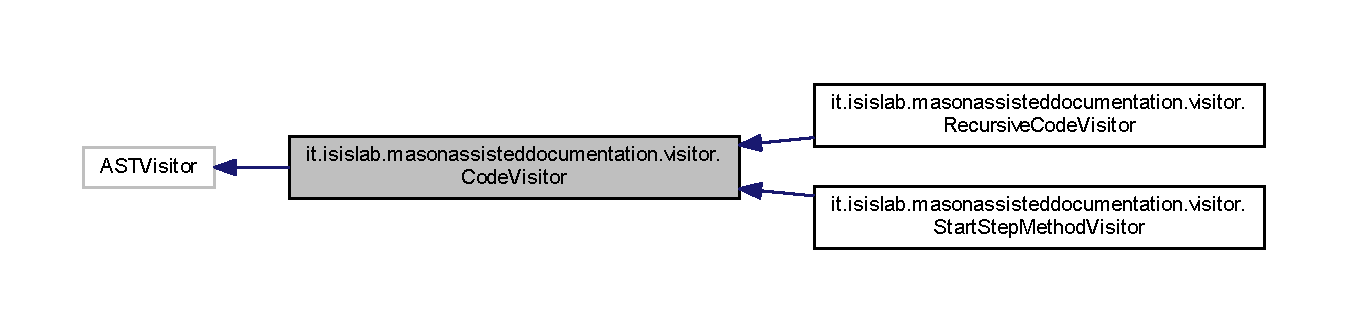
\includegraphics[width=350pt]{classit_1_1isislab_1_1masonassisteddocumentation_1_1visitor_1_1_code_visitor__inherit__graph}
\end{center}
\end{figure}


Collaboration diagram for it.\-isislab.\-masonassisteddocumentation.\-visitor.\-Code\-Visitor\-:\nopagebreak
\begin{figure}[H]
\begin{center}
\leavevmode
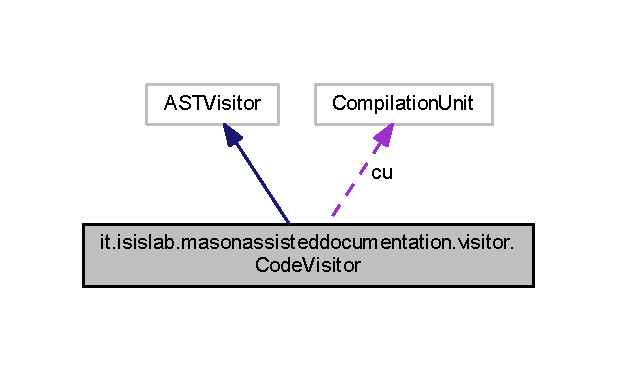
\includegraphics[width=296pt]{classit_1_1isislab_1_1masonassisteddocumentation_1_1visitor_1_1_code_visitor__coll__graph}
\end{center}
\end{figure}
\subsection*{Public Member Functions}
\begin{DoxyCompactItemize}
\item 
\hyperlink{classit_1_1isislab_1_1masonassisteddocumentation_1_1visitor_1_1_code_visitor_a23012a94a2c90abe9c89b241d11ce586}{Code\-Visitor} (Compilation\-Unit \hyperlink{classit_1_1isislab_1_1masonassisteddocumentation_1_1visitor_1_1_code_visitor_ad567a4c5516729e6ad3c520b779e5fbf}{cu})
\item 
boolean \hyperlink{classit_1_1isislab_1_1masonassisteddocumentation_1_1visitor_1_1_code_visitor_a2cf8c545b996ca299f1767f77b4c9c8f}{visit} (If\-Statement node)
\item 
void \hyperlink{classit_1_1isislab_1_1masonassisteddocumentation_1_1visitor_1_1_code_visitor_a69c11f1c13b49c21a1fdc5b9131e82db}{end\-Visit} (If\-Statement node)
\item 
boolean \hyperlink{classit_1_1isislab_1_1masonassisteddocumentation_1_1visitor_1_1_code_visitor_ad03bbbf8800ecf154acc28a75a79ad7b}{visit} (For\-Statement f)
\item 
void \hyperlink{classit_1_1isislab_1_1masonassisteddocumentation_1_1visitor_1_1_code_visitor_a60512fd6a6d5601b1977bbe39407522b}{end\-Visit} (For\-Statement node)
\item 
boolean \hyperlink{classit_1_1isislab_1_1masonassisteddocumentation_1_1visitor_1_1_code_visitor_ad97a8e87a73d80a3be2cbf784ceee731}{visit} (Do\-Statement d)
\item 
void \hyperlink{classit_1_1isislab_1_1masonassisteddocumentation_1_1visitor_1_1_code_visitor_a635c2ee5422e31fb4eac22ba3a828244}{end\-Visit} (Do\-Statement node)
\item 
boolean \hyperlink{classit_1_1isislab_1_1masonassisteddocumentation_1_1visitor_1_1_code_visitor_aea58bf6bc0baf1f20a85bf715cfa07da}{visit} (Switch\-Statement s)
\item 
void \hyperlink{classit_1_1isislab_1_1masonassisteddocumentation_1_1visitor_1_1_code_visitor_aba38ab15bd632a6cedb45db36a4c0abd}{end\-Visit} (Switch\-Statement node)
\item 
boolean \hyperlink{classit_1_1isislab_1_1masonassisteddocumentation_1_1visitor_1_1_code_visitor_aed58991441b8cdbddd6c17c732bcece6}{visit} (Type\-Declaration t)
\item 
void \hyperlink{classit_1_1isislab_1_1masonassisteddocumentation_1_1visitor_1_1_code_visitor_a8aa7283c1529d856a5c4f44a20ac0d5b}{end\-Visit} (Type\-Declaration node)
\item 
boolean \hyperlink{classit_1_1isislab_1_1masonassisteddocumentation_1_1visitor_1_1_code_visitor_a802b2916ebe1045fd32be378ad5fdc89}{visit} (Assignment node)
\item 
void \hyperlink{classit_1_1isislab_1_1masonassisteddocumentation_1_1visitor_1_1_code_visitor_a02060c3318faa3bbd19f4517ca2b6843}{end\-Visit} (Assignment node)
\item 
void \hyperlink{classit_1_1isislab_1_1masonassisteddocumentation_1_1visitor_1_1_code_visitor_aefe7e1dfda4f465845e03407a198ccc2}{end\-Visit} (Method\-Invocation node)
\item 
String \hyperlink{classit_1_1isislab_1_1masonassisteddocumentation_1_1visitor_1_1_code_visitor_aa68511a2fe4ebc5c8dca3694ddd072ed}{get\-Information\-\_\-s} ()
\item 
abstract boolean \hyperlink{classit_1_1isislab_1_1masonassisteddocumentation_1_1visitor_1_1_code_visitor_aa4e0bbbc1f0226abcf00be8c384a18fb}{visit} (Method\-Invocation node)
\end{DoxyCompactItemize}
\subsection*{Protected Attributes}
\begin{DoxyCompactItemize}
\item 
String \hyperlink{classit_1_1isislab_1_1masonassisteddocumentation_1_1visitor_1_1_code_visitor_a628ab846d2f4de647f171060ebe73774}{information\-\_\-s}
\end{DoxyCompactItemize}
\subsection*{Private Member Functions}
\begin{DoxyCompactItemize}
\item 
void \hyperlink{classit_1_1isislab_1_1masonassisteddocumentation_1_1visitor_1_1_code_visitor_a31af3e78c358dfc103b9ed9348fba615}{add\-Some\-New\-Line} ()
\end{DoxyCompactItemize}
\subsection*{Private Attributes}
\begin{DoxyCompactItemize}
\item 
Compilation\-Unit \hyperlink{classit_1_1isislab_1_1masonassisteddocumentation_1_1visitor_1_1_code_visitor_ad567a4c5516729e6ad3c520b779e5fbf}{cu}
\end{DoxyCompactItemize}


\subsection{Constructor \& Destructor Documentation}
\hypertarget{classit_1_1isislab_1_1masonassisteddocumentation_1_1visitor_1_1_code_visitor_a23012a94a2c90abe9c89b241d11ce586}{\index{it\-::isislab\-::masonassisteddocumentation\-::visitor\-::\-Code\-Visitor@{it\-::isislab\-::masonassisteddocumentation\-::visitor\-::\-Code\-Visitor}!Code\-Visitor@{Code\-Visitor}}
\index{Code\-Visitor@{Code\-Visitor}!it::isislab::masonassisteddocumentation::visitor::CodeVisitor@{it\-::isislab\-::masonassisteddocumentation\-::visitor\-::\-Code\-Visitor}}
\subsubsection[{Code\-Visitor}]{\setlength{\rightskip}{0pt plus 5cm}it.\-isislab.\-masonassisteddocumentation.\-visitor.\-Code\-Visitor.\-Code\-Visitor (
\begin{DoxyParamCaption}
\item[{Compilation\-Unit}]{cu}
\end{DoxyParamCaption}
)}}\label{classit_1_1isislab_1_1masonassisteddocumentation_1_1visitor_1_1_code_visitor_a23012a94a2c90abe9c89b241d11ce586}

\begin{DoxyCode}
18                                           \{
19         this.cu = \hyperlink{classit_1_1isislab_1_1masonassisteddocumentation_1_1visitor_1_1_code_visitor_ad567a4c5516729e6ad3c520b779e5fbf}{cu};
20         \hyperlink{classit_1_1isislab_1_1masonassisteddocumentation_1_1visitor_1_1_code_visitor_a628ab846d2f4de647f171060ebe73774}{information\_s} = \textcolor{stringliteral}{""};
21     \}
\end{DoxyCode}


\subsection{Member Function Documentation}
\hypertarget{classit_1_1isislab_1_1masonassisteddocumentation_1_1visitor_1_1_code_visitor_a31af3e78c358dfc103b9ed9348fba615}{\index{it\-::isislab\-::masonassisteddocumentation\-::visitor\-::\-Code\-Visitor@{it\-::isislab\-::masonassisteddocumentation\-::visitor\-::\-Code\-Visitor}!add\-Some\-New\-Line@{add\-Some\-New\-Line}}
\index{add\-Some\-New\-Line@{add\-Some\-New\-Line}!it::isislab::masonassisteddocumentation::visitor::CodeVisitor@{it\-::isislab\-::masonassisteddocumentation\-::visitor\-::\-Code\-Visitor}}
\subsubsection[{add\-Some\-New\-Line}]{\setlength{\rightskip}{0pt plus 5cm}void it.\-isislab.\-masonassisteddocumentation.\-visitor.\-Code\-Visitor.\-add\-Some\-New\-Line (
\begin{DoxyParamCaption}
{}
\end{DoxyParamCaption}
)\hspace{0.3cm}{\ttfamily [private]}}}\label{classit_1_1isislab_1_1masonassisteddocumentation_1_1visitor_1_1_code_visitor_a31af3e78c358dfc103b9ed9348fba615}
This method add '\par
' each 8 white space. 
\begin{DoxyCode}
90                                   \{
91         \textcolor{keywordtype}{int} eachNumSpace = 8;
92         \textcolor{keywordtype}{int} spaceCounter = 0;
93         StringBuilder result = \textcolor{keyword}{new} StringBuilder(\hyperlink{classit_1_1isislab_1_1masonassisteddocumentation_1_1visitor_1_1_code_visitor_a628ab846d2f4de647f171060ebe73774}{information\_s});
94         \textcolor{keywordflow}{for} (\textcolor{keywordtype}{int} i=0; i<information\_s.length(); i++)\{
95             \textcolor{keywordflow}{if} (\hyperlink{classit_1_1isislab_1_1masonassisteddocumentation_1_1visitor_1_1_code_visitor_a628ab846d2f4de647f171060ebe73774}{information\_s}.charAt(i) == \textcolor{charliteral}{' '})\{
96                 spaceCounter++;
97                 \textcolor{keywordflow}{if} (spaceCounter >= eachNumSpace)\{
98                     result.setCharAt(i, \textcolor{charliteral}{'\(\backslash\)n'});
99                     spaceCounter = 0;
100                 \}
101             \}
102         \}
103         \hyperlink{classit_1_1isislab_1_1masonassisteddocumentation_1_1visitor_1_1_code_visitor_a628ab846d2f4de647f171060ebe73774}{information\_s} = result.toString();
104     \}
\end{DoxyCode}
\hypertarget{classit_1_1isislab_1_1masonassisteddocumentation_1_1visitor_1_1_code_visitor_a69c11f1c13b49c21a1fdc5b9131e82db}{\index{it\-::isislab\-::masonassisteddocumentation\-::visitor\-::\-Code\-Visitor@{it\-::isislab\-::masonassisteddocumentation\-::visitor\-::\-Code\-Visitor}!end\-Visit@{end\-Visit}}
\index{end\-Visit@{end\-Visit}!it::isislab::masonassisteddocumentation::visitor::CodeVisitor@{it\-::isislab\-::masonassisteddocumentation\-::visitor\-::\-Code\-Visitor}}
\subsubsection[{end\-Visit}]{\setlength{\rightskip}{0pt plus 5cm}void it.\-isislab.\-masonassisteddocumentation.\-visitor.\-Code\-Visitor.\-end\-Visit (
\begin{DoxyParamCaption}
\item[{If\-Statement}]{node}
\end{DoxyParamCaption}
)}}\label{classit_1_1isislab_1_1masonassisteddocumentation_1_1visitor_1_1_code_visitor_a69c11f1c13b49c21a1fdc5b9131e82db}

\begin{DoxyCode}
29                                           \{
30         \hyperlink{classit_1_1isislab_1_1masonassisteddocumentation_1_1visitor_1_1_code_visitor_a628ab846d2f4de647f171060ebe73774}{information\_s} += \hyperlink{classit_1_1isislab_1_1masonassisteddocumentation_1_1visitor_1_1_messages_a1ed1017869268de698f98b7fa1c28ef3}{Messages.Visitor\_EndIf};
31     \}
\end{DoxyCode}
\hypertarget{classit_1_1isislab_1_1masonassisteddocumentation_1_1visitor_1_1_code_visitor_a60512fd6a6d5601b1977bbe39407522b}{\index{it\-::isislab\-::masonassisteddocumentation\-::visitor\-::\-Code\-Visitor@{it\-::isislab\-::masonassisteddocumentation\-::visitor\-::\-Code\-Visitor}!end\-Visit@{end\-Visit}}
\index{end\-Visit@{end\-Visit}!it::isislab::masonassisteddocumentation::visitor::CodeVisitor@{it\-::isislab\-::masonassisteddocumentation\-::visitor\-::\-Code\-Visitor}}
\subsubsection[{end\-Visit}]{\setlength{\rightskip}{0pt plus 5cm}void it.\-isislab.\-masonassisteddocumentation.\-visitor.\-Code\-Visitor.\-end\-Visit (
\begin{DoxyParamCaption}
\item[{For\-Statement}]{node}
\end{DoxyParamCaption}
)}}\label{classit_1_1isislab_1_1masonassisteddocumentation_1_1visitor_1_1_code_visitor_a60512fd6a6d5601b1977bbe39407522b}

\begin{DoxyCode}
38                                            \{
39         \hyperlink{classit_1_1isislab_1_1masonassisteddocumentation_1_1visitor_1_1_code_visitor_a628ab846d2f4de647f171060ebe73774}{information\_s} += \hyperlink{classit_1_1isislab_1_1masonassisteddocumentation_1_1visitor_1_1_messages_a2fa6faeb6b5b086b3cb1a856b4f42e40}{Messages.Visitor\_EndFor}; \textcolor{comment}{//$NON-NLS-2$;}
40     \}
\end{DoxyCode}
\hypertarget{classit_1_1isislab_1_1masonassisteddocumentation_1_1visitor_1_1_code_visitor_a635c2ee5422e31fb4eac22ba3a828244}{\index{it\-::isislab\-::masonassisteddocumentation\-::visitor\-::\-Code\-Visitor@{it\-::isislab\-::masonassisteddocumentation\-::visitor\-::\-Code\-Visitor}!end\-Visit@{end\-Visit}}
\index{end\-Visit@{end\-Visit}!it::isislab::masonassisteddocumentation::visitor::CodeVisitor@{it\-::isislab\-::masonassisteddocumentation\-::visitor\-::\-Code\-Visitor}}
\subsubsection[{end\-Visit}]{\setlength{\rightskip}{0pt plus 5cm}void it.\-isislab.\-masonassisteddocumentation.\-visitor.\-Code\-Visitor.\-end\-Visit (
\begin{DoxyParamCaption}
\item[{Do\-Statement}]{node}
\end{DoxyParamCaption}
)}}\label{classit_1_1isislab_1_1masonassisteddocumentation_1_1visitor_1_1_code_visitor_a635c2ee5422e31fb4eac22ba3a828244}

\begin{DoxyCode}
47                                           \{
48         \hyperlink{classit_1_1isislab_1_1masonassisteddocumentation_1_1visitor_1_1_code_visitor_a628ab846d2f4de647f171060ebe73774}{information\_s} += \hyperlink{classit_1_1isislab_1_1masonassisteddocumentation_1_1visitor_1_1_messages_a71859117ad5199260686a200b2cc6d0a}{Messages.Visitor\_DoWhileEnd};
49     \}
\end{DoxyCode}
\hypertarget{classit_1_1isislab_1_1masonassisteddocumentation_1_1visitor_1_1_code_visitor_aba38ab15bd632a6cedb45db36a4c0abd}{\index{it\-::isislab\-::masonassisteddocumentation\-::visitor\-::\-Code\-Visitor@{it\-::isislab\-::masonassisteddocumentation\-::visitor\-::\-Code\-Visitor}!end\-Visit@{end\-Visit}}
\index{end\-Visit@{end\-Visit}!it::isislab::masonassisteddocumentation::visitor::CodeVisitor@{it\-::isislab\-::masonassisteddocumentation\-::visitor\-::\-Code\-Visitor}}
\subsubsection[{end\-Visit}]{\setlength{\rightskip}{0pt plus 5cm}void it.\-isislab.\-masonassisteddocumentation.\-visitor.\-Code\-Visitor.\-end\-Visit (
\begin{DoxyParamCaption}
\item[{Switch\-Statement}]{node}
\end{DoxyParamCaption}
)}}\label{classit_1_1isislab_1_1masonassisteddocumentation_1_1visitor_1_1_code_visitor_aba38ab15bd632a6cedb45db36a4c0abd}

\begin{DoxyCode}
56                                               \{
57         \hyperlink{classit_1_1isislab_1_1masonassisteddocumentation_1_1visitor_1_1_code_visitor_a628ab846d2f4de647f171060ebe73774}{information\_s} += \hyperlink{classit_1_1isislab_1_1masonassisteddocumentation_1_1visitor_1_1_messages_a61780577c25f50256403622b34fb9126}{Messages.Visitor\_EndSwitch};
58     \}
\end{DoxyCode}
\hypertarget{classit_1_1isislab_1_1masonassisteddocumentation_1_1visitor_1_1_code_visitor_a8aa7283c1529d856a5c4f44a20ac0d5b}{\index{it\-::isislab\-::masonassisteddocumentation\-::visitor\-::\-Code\-Visitor@{it\-::isislab\-::masonassisteddocumentation\-::visitor\-::\-Code\-Visitor}!end\-Visit@{end\-Visit}}
\index{end\-Visit@{end\-Visit}!it::isislab::masonassisteddocumentation::visitor::CodeVisitor@{it\-::isislab\-::masonassisteddocumentation\-::visitor\-::\-Code\-Visitor}}
\subsubsection[{end\-Visit}]{\setlength{\rightskip}{0pt plus 5cm}void it.\-isislab.\-masonassisteddocumentation.\-visitor.\-Code\-Visitor.\-end\-Visit (
\begin{DoxyParamCaption}
\item[{Type\-Declaration}]{node}
\end{DoxyParamCaption}
)}}\label{classit_1_1isislab_1_1masonassisteddocumentation_1_1visitor_1_1_code_visitor_a8aa7283c1529d856a5c4f44a20ac0d5b}

\begin{DoxyCode}
65                                               \{
66         \hyperlink{classit_1_1isislab_1_1masonassisteddocumentation_1_1visitor_1_1_code_visitor_a628ab846d2f4de647f171060ebe73774}{information\_s} += \hyperlink{classit_1_1isislab_1_1masonassisteddocumentation_1_1visitor_1_1_messages_aa35b09165711d8325fbb946a235ee338}{Messages.Visitor\_EndTypeDeclaration}
      ;
67     \}
\end{DoxyCode}
\hypertarget{classit_1_1isislab_1_1masonassisteddocumentation_1_1visitor_1_1_code_visitor_a02060c3318faa3bbd19f4517ca2b6843}{\index{it\-::isislab\-::masonassisteddocumentation\-::visitor\-::\-Code\-Visitor@{it\-::isislab\-::masonassisteddocumentation\-::visitor\-::\-Code\-Visitor}!end\-Visit@{end\-Visit}}
\index{end\-Visit@{end\-Visit}!it::isislab::masonassisteddocumentation::visitor::CodeVisitor@{it\-::isislab\-::masonassisteddocumentation\-::visitor\-::\-Code\-Visitor}}
\subsubsection[{end\-Visit}]{\setlength{\rightskip}{0pt plus 5cm}void it.\-isislab.\-masonassisteddocumentation.\-visitor.\-Code\-Visitor.\-end\-Visit (
\begin{DoxyParamCaption}
\item[{Assignment}]{node}
\end{DoxyParamCaption}
)}}\label{classit_1_1isislab_1_1masonassisteddocumentation_1_1visitor_1_1_code_visitor_a02060c3318faa3bbd19f4517ca2b6843}

\begin{DoxyCode}
74                                          \{
75         \hyperlink{classit_1_1isislab_1_1masonassisteddocumentation_1_1visitor_1_1_code_visitor_a628ab846d2f4de647f171060ebe73774}{information\_s} += \hyperlink{classit_1_1isislab_1_1masonassisteddocumentation_1_1visitor_1_1_messages_acdd892597a5ade9c9518f5a12b31213d}{Messages.Visitor\_EndAssignent};
76     \}
\end{DoxyCode}
\hypertarget{classit_1_1isislab_1_1masonassisteddocumentation_1_1visitor_1_1_code_visitor_aefe7e1dfda4f465845e03407a198ccc2}{\index{it\-::isislab\-::masonassisteddocumentation\-::visitor\-::\-Code\-Visitor@{it\-::isislab\-::masonassisteddocumentation\-::visitor\-::\-Code\-Visitor}!end\-Visit@{end\-Visit}}
\index{end\-Visit@{end\-Visit}!it::isislab::masonassisteddocumentation::visitor::CodeVisitor@{it\-::isislab\-::masonassisteddocumentation\-::visitor\-::\-Code\-Visitor}}
\subsubsection[{end\-Visit}]{\setlength{\rightskip}{0pt plus 5cm}void it.\-isislab.\-masonassisteddocumentation.\-visitor.\-Code\-Visitor.\-end\-Visit (
\begin{DoxyParamCaption}
\item[{Method\-Invocation}]{node}
\end{DoxyParamCaption}
)}}\label{classit_1_1isislab_1_1masonassisteddocumentation_1_1visitor_1_1_code_visitor_aefe7e1dfda4f465845e03407a198ccc2}

\begin{DoxyCode}
79                                                \{
80         \hyperlink{classit_1_1isislab_1_1masonassisteddocumentation_1_1visitor_1_1_code_visitor_a628ab846d2f4de647f171060ebe73774}{information\_s} += Messages.Visitor\_EndInvocation + node.getName() + Messages.
      Visitor\_EndInvocation1;
81     \}
\end{DoxyCode}
\hypertarget{classit_1_1isislab_1_1masonassisteddocumentation_1_1visitor_1_1_code_visitor_aa68511a2fe4ebc5c8dca3694ddd072ed}{\index{it\-::isislab\-::masonassisteddocumentation\-::visitor\-::\-Code\-Visitor@{it\-::isislab\-::masonassisteddocumentation\-::visitor\-::\-Code\-Visitor}!get\-Information\-\_\-s@{get\-Information\-\_\-s}}
\index{get\-Information\-\_\-s@{get\-Information\-\_\-s}!it::isislab::masonassisteddocumentation::visitor::CodeVisitor@{it\-::isislab\-::masonassisteddocumentation\-::visitor\-::\-Code\-Visitor}}
\subsubsection[{get\-Information\-\_\-s}]{\setlength{\rightskip}{0pt plus 5cm}String it.\-isislab.\-masonassisteddocumentation.\-visitor.\-Code\-Visitor.\-get\-Information\-\_\-s (
\begin{DoxyParamCaption}
{}
\end{DoxyParamCaption}
)}}\label{classit_1_1isislab_1_1masonassisteddocumentation_1_1visitor_1_1_code_visitor_aa68511a2fe4ebc5c8dca3694ddd072ed}

\begin{DoxyCode}
83                                      \{
84         \textcolor{keywordflow}{return} \hyperlink{classit_1_1isislab_1_1masonassisteddocumentation_1_1visitor_1_1_code_visitor_a628ab846d2f4de647f171060ebe73774}{information\_s} + \hyperlink{classit_1_1isislab_1_1masonassisteddocumentation_1_1visitor_1_1_messages_aa15f6df87f0c39b06d1900e6b1621a5b}{Messages.Visitor\_EndMethod};
85     \}
\end{DoxyCode}
\hypertarget{classit_1_1isislab_1_1masonassisteddocumentation_1_1visitor_1_1_code_visitor_a2cf8c545b996ca299f1767f77b4c9c8f}{\index{it\-::isislab\-::masonassisteddocumentation\-::visitor\-::\-Code\-Visitor@{it\-::isislab\-::masonassisteddocumentation\-::visitor\-::\-Code\-Visitor}!visit@{visit}}
\index{visit@{visit}!it::isislab::masonassisteddocumentation::visitor::CodeVisitor@{it\-::isislab\-::masonassisteddocumentation\-::visitor\-::\-Code\-Visitor}}
\subsubsection[{visit}]{\setlength{\rightskip}{0pt plus 5cm}boolean it.\-isislab.\-masonassisteddocumentation.\-visitor.\-Code\-Visitor.\-visit (
\begin{DoxyParamCaption}
\item[{If\-Statement}]{node}
\end{DoxyParamCaption}
)}}\label{classit_1_1isislab_1_1masonassisteddocumentation_1_1visitor_1_1_code_visitor_a2cf8c545b996ca299f1767f77b4c9c8f}

\begin{DoxyCode}
24                                            \{
25         \hyperlink{classit_1_1isislab_1_1masonassisteddocumentation_1_1visitor_1_1_code_visitor_a628ab846d2f4de647f171060ebe73774}{information\_s} += Messages.Visitor\_If1 + node.getExpression() + \textcolor{stringliteral}{" "}; \textcolor{comment}{//$NON-NLS-2$}
26         \textcolor{keywordflow}{return} super.visit(node);
27     \}
\end{DoxyCode}
\hypertarget{classit_1_1isislab_1_1masonassisteddocumentation_1_1visitor_1_1_code_visitor_ad03bbbf8800ecf154acc28a75a79ad7b}{\index{it\-::isislab\-::masonassisteddocumentation\-::visitor\-::\-Code\-Visitor@{it\-::isislab\-::masonassisteddocumentation\-::visitor\-::\-Code\-Visitor}!visit@{visit}}
\index{visit@{visit}!it::isislab::masonassisteddocumentation::visitor::CodeVisitor@{it\-::isislab\-::masonassisteddocumentation\-::visitor\-::\-Code\-Visitor}}
\subsubsection[{visit}]{\setlength{\rightskip}{0pt plus 5cm}boolean it.\-isislab.\-masonassisteddocumentation.\-visitor.\-Code\-Visitor.\-visit (
\begin{DoxyParamCaption}
\item[{For\-Statement}]{f}
\end{DoxyParamCaption}
)}}\label{classit_1_1isislab_1_1masonassisteddocumentation_1_1visitor_1_1_code_visitor_ad03bbbf8800ecf154acc28a75a79ad7b}

\begin{DoxyCode}
33                                         \{
34         \hyperlink{classit_1_1isislab_1_1masonassisteddocumentation_1_1visitor_1_1_code_visitor_a628ab846d2f4de647f171060ebe73774}{information\_s} += Messages.Visitor\_While1 + f.getExpression() + \textcolor{stringliteral}{" "}; \textcolor{comment}{//$NON-NLS-2$}
35         \textcolor{keywordflow}{return} super.visit(f);
36     \}
\end{DoxyCode}
\hypertarget{classit_1_1isislab_1_1masonassisteddocumentation_1_1visitor_1_1_code_visitor_ad97a8e87a73d80a3be2cbf784ceee731}{\index{it\-::isislab\-::masonassisteddocumentation\-::visitor\-::\-Code\-Visitor@{it\-::isislab\-::masonassisteddocumentation\-::visitor\-::\-Code\-Visitor}!visit@{visit}}
\index{visit@{visit}!it::isislab::masonassisteddocumentation::visitor::CodeVisitor@{it\-::isislab\-::masonassisteddocumentation\-::visitor\-::\-Code\-Visitor}}
\subsubsection[{visit}]{\setlength{\rightskip}{0pt plus 5cm}boolean it.\-isislab.\-masonassisteddocumentation.\-visitor.\-Code\-Visitor.\-visit (
\begin{DoxyParamCaption}
\item[{Do\-Statement}]{d}
\end{DoxyParamCaption}
)}}\label{classit_1_1isislab_1_1masonassisteddocumentation_1_1visitor_1_1_code_visitor_ad97a8e87a73d80a3be2cbf784ceee731}

\begin{DoxyCode}
42                                         \{
43         \hyperlink{classit_1_1isislab_1_1masonassisteddocumentation_1_1visitor_1_1_code_visitor_a628ab846d2f4de647f171060ebe73774}{information\_s} += Messages.Visitor\_Do1 + d.getExpression() + \textcolor{stringliteral}{" "}; \textcolor{comment}{//$NON-NLS-2$}
44         \textcolor{keywordflow}{return} super.visit(d);
45     \}
\end{DoxyCode}
\hypertarget{classit_1_1isislab_1_1masonassisteddocumentation_1_1visitor_1_1_code_visitor_aea58bf6bc0baf1f20a85bf715cfa07da}{\index{it\-::isislab\-::masonassisteddocumentation\-::visitor\-::\-Code\-Visitor@{it\-::isislab\-::masonassisteddocumentation\-::visitor\-::\-Code\-Visitor}!visit@{visit}}
\index{visit@{visit}!it::isislab::masonassisteddocumentation::visitor::CodeVisitor@{it\-::isislab\-::masonassisteddocumentation\-::visitor\-::\-Code\-Visitor}}
\subsubsection[{visit}]{\setlength{\rightskip}{0pt plus 5cm}boolean it.\-isislab.\-masonassisteddocumentation.\-visitor.\-Code\-Visitor.\-visit (
\begin{DoxyParamCaption}
\item[{Switch\-Statement}]{s}
\end{DoxyParamCaption}
)}}\label{classit_1_1isislab_1_1masonassisteddocumentation_1_1visitor_1_1_code_visitor_aea58bf6bc0baf1f20a85bf715cfa07da}

\begin{DoxyCode}
51                                            \{
52         \hyperlink{classit_1_1isislab_1_1masonassisteddocumentation_1_1visitor_1_1_code_visitor_a628ab846d2f4de647f171060ebe73774}{information\_s} += Messages.Visitor\_SwitchInfo + s.getExpression() + \textcolor{stringliteral}{" "}; \textcolor{comment}{//$NON-NLS-2$}
53         \textcolor{keywordflow}{return} super.visit(s);
54     \}
\end{DoxyCode}
\hypertarget{classit_1_1isislab_1_1masonassisteddocumentation_1_1visitor_1_1_code_visitor_aed58991441b8cdbddd6c17c732bcece6}{\index{it\-::isislab\-::masonassisteddocumentation\-::visitor\-::\-Code\-Visitor@{it\-::isislab\-::masonassisteddocumentation\-::visitor\-::\-Code\-Visitor}!visit@{visit}}
\index{visit@{visit}!it::isislab::masonassisteddocumentation::visitor::CodeVisitor@{it\-::isislab\-::masonassisteddocumentation\-::visitor\-::\-Code\-Visitor}}
\subsubsection[{visit}]{\setlength{\rightskip}{0pt plus 5cm}boolean it.\-isislab.\-masonassisteddocumentation.\-visitor.\-Code\-Visitor.\-visit (
\begin{DoxyParamCaption}
\item[{Type\-Declaration}]{t}
\end{DoxyParamCaption}
)}}\label{classit_1_1isislab_1_1masonassisteddocumentation_1_1visitor_1_1_code_visitor_aed58991441b8cdbddd6c17c732bcece6}

\begin{DoxyCode}
60                                            \{
61         \hyperlink{classit_1_1isislab_1_1masonassisteddocumentation_1_1visitor_1_1_code_visitor_a628ab846d2f4de647f171060ebe73774}{information\_s} += Messages.Visitor\_TypeDeclaration + t.getName();
62         \textcolor{keywordflow}{return} super.visit(t);
63     \}
\end{DoxyCode}
\hypertarget{classit_1_1isislab_1_1masonassisteddocumentation_1_1visitor_1_1_code_visitor_a802b2916ebe1045fd32be378ad5fdc89}{\index{it\-::isislab\-::masonassisteddocumentation\-::visitor\-::\-Code\-Visitor@{it\-::isislab\-::masonassisteddocumentation\-::visitor\-::\-Code\-Visitor}!visit@{visit}}
\index{visit@{visit}!it::isislab::masonassisteddocumentation::visitor::CodeVisitor@{it\-::isislab\-::masonassisteddocumentation\-::visitor\-::\-Code\-Visitor}}
\subsubsection[{visit}]{\setlength{\rightskip}{0pt plus 5cm}boolean it.\-isislab.\-masonassisteddocumentation.\-visitor.\-Code\-Visitor.\-visit (
\begin{DoxyParamCaption}
\item[{Assignment}]{node}
\end{DoxyParamCaption}
)}}\label{classit_1_1isislab_1_1masonassisteddocumentation_1_1visitor_1_1_code_visitor_a802b2916ebe1045fd32be378ad5fdc89}

\begin{DoxyCode}
69                                          \{
70         \hyperlink{classit_1_1isislab_1_1masonassisteddocumentation_1_1visitor_1_1_code_visitor_a628ab846d2f4de647f171060ebe73774}{information\_s} += Messages.Visitor\_Assignment + node.getLeftHandSide() + Messages.
      Visitor\_Assignemnt1 + node.getRightHandSide() + \textcolor{stringliteral}{"."}; \textcolor{comment}{//$NON-NLS-3$}
71         \textcolor{keywordflow}{return} super.visit(node);
72     \}
\end{DoxyCode}
\hypertarget{classit_1_1isislab_1_1masonassisteddocumentation_1_1visitor_1_1_code_visitor_aa4e0bbbc1f0226abcf00be8c384a18fb}{\index{it\-::isislab\-::masonassisteddocumentation\-::visitor\-::\-Code\-Visitor@{it\-::isislab\-::masonassisteddocumentation\-::visitor\-::\-Code\-Visitor}!visit@{visit}}
\index{visit@{visit}!it::isislab::masonassisteddocumentation::visitor::CodeVisitor@{it\-::isislab\-::masonassisteddocumentation\-::visitor\-::\-Code\-Visitor}}
\subsubsection[{visit}]{\setlength{\rightskip}{0pt plus 5cm}abstract boolean it.\-isislab.\-masonassisteddocumentation.\-visitor.\-Code\-Visitor.\-visit (
\begin{DoxyParamCaption}
\item[{Method\-Invocation}]{node}
\end{DoxyParamCaption}
)\hspace{0.3cm}{\ttfamily [abstract]}}}\label{classit_1_1isislab_1_1masonassisteddocumentation_1_1visitor_1_1_code_visitor_aa4e0bbbc1f0226abcf00be8c384a18fb}


\subsection{Member Data Documentation}
\hypertarget{classit_1_1isislab_1_1masonassisteddocumentation_1_1visitor_1_1_code_visitor_ad567a4c5516729e6ad3c520b779e5fbf}{\index{it\-::isislab\-::masonassisteddocumentation\-::visitor\-::\-Code\-Visitor@{it\-::isislab\-::masonassisteddocumentation\-::visitor\-::\-Code\-Visitor}!cu@{cu}}
\index{cu@{cu}!it::isislab::masonassisteddocumentation::visitor::CodeVisitor@{it\-::isislab\-::masonassisteddocumentation\-::visitor\-::\-Code\-Visitor}}
\subsubsection[{cu}]{\setlength{\rightskip}{0pt plus 5cm}Compilation\-Unit it.\-isislab.\-masonassisteddocumentation.\-visitor.\-Code\-Visitor.\-cu\hspace{0.3cm}{\ttfamily [private]}}}\label{classit_1_1isislab_1_1masonassisteddocumentation_1_1visitor_1_1_code_visitor_ad567a4c5516729e6ad3c520b779e5fbf}
\hypertarget{classit_1_1isislab_1_1masonassisteddocumentation_1_1visitor_1_1_code_visitor_a628ab846d2f4de647f171060ebe73774}{\index{it\-::isislab\-::masonassisteddocumentation\-::visitor\-::\-Code\-Visitor@{it\-::isislab\-::masonassisteddocumentation\-::visitor\-::\-Code\-Visitor}!information\-\_\-s@{information\-\_\-s}}
\index{information\-\_\-s@{information\-\_\-s}!it::isislab::masonassisteddocumentation::visitor::CodeVisitor@{it\-::isislab\-::masonassisteddocumentation\-::visitor\-::\-Code\-Visitor}}
\subsubsection[{information\-\_\-s}]{\setlength{\rightskip}{0pt plus 5cm}String it.\-isislab.\-masonassisteddocumentation.\-visitor.\-Code\-Visitor.\-information\-\_\-s\hspace{0.3cm}{\ttfamily [protected]}}}\label{classit_1_1isislab_1_1masonassisteddocumentation_1_1visitor_1_1_code_visitor_a628ab846d2f4de647f171060ebe73774}


The documentation for this class was generated from the following file\-:\begin{DoxyCompactItemize}
\item 
src/it/isislab/masonassisteddocumentation/visitor/\hyperlink{_code_visitor_8java}{Code\-Visitor.\-java}\end{DoxyCompactItemize}

\hypertarget{classit_1_1isislab_1_1masonassisteddocumentation_1_1mason_1_1control_1_1_config_file}{\section{it.\-isislab.\-masonassisteddocumentation.\-mason.\-control.\-Config\-File Class Reference}
\label{classit_1_1isislab_1_1masonassisteddocumentation_1_1mason_1_1control_1_1_config_file}\index{it.\-isislab.\-masonassisteddocumentation.\-mason.\-control.\-Config\-File@{it.\-isislab.\-masonassisteddocumentation.\-mason.\-control.\-Config\-File}}
}


Collaboration diagram for it.\-isislab.\-masonassisteddocumentation.\-mason.\-control.\-Config\-File\-:\nopagebreak
\begin{figure}[H]
\begin{center}
\leavevmode
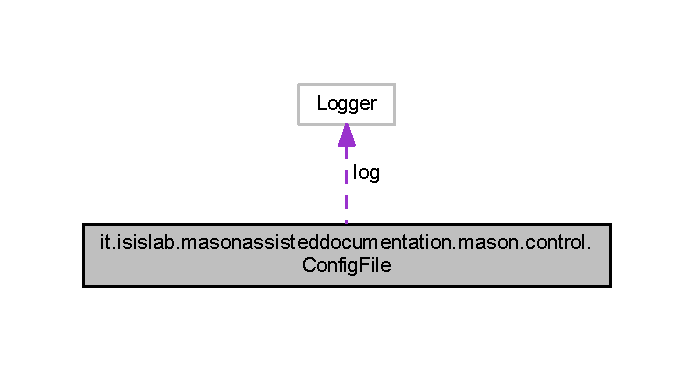
\includegraphics[width=333pt]{classit_1_1isislab_1_1masonassisteddocumentation_1_1mason_1_1control_1_1_config_file__coll__graph}
\end{center}
\end{figure}
\subsection*{Static Public Member Functions}
\begin{DoxyCompactItemize}
\item 
static String \hyperlink{classit_1_1isislab_1_1masonassisteddocumentation_1_1mason_1_1control_1_1_config_file_add444e913763f18b80005e5ad477c59d}{get\-Project\-\_\-s\-Dir\-Path} ()
\item 
static String \hyperlink{classit_1_1isislab_1_1masonassisteddocumentation_1_1mason_1_1control_1_1_config_file_a67bf373e54fb3ce5144d6f4fcbb48bfd}{get\-Project\-Dir} ()
\item 
static String \hyperlink{classit_1_1isislab_1_1masonassisteddocumentation_1_1mason_1_1control_1_1_config_file_a0bc9608fcc97bf301d3529c9ee9ae5f8}{get\-Source\-Backup\-Dir} ()
\item 
static void \hyperlink{classit_1_1isislab_1_1masonassisteddocumentation_1_1mason_1_1control_1_1_config_file_ae68816366df216e1d9525047c91e77fc}{set\-Property} (String key, String value)
\item 
static String \hyperlink{classit_1_1isislab_1_1masonassisteddocumentation_1_1mason_1_1control_1_1_config_file_abb43073f42616e4349b2fcb4e964c648}{get\-Value} (String key)
\item 
static String \hyperlink{classit_1_1isislab_1_1masonassisteddocumentation_1_1mason_1_1control_1_1_config_file_a69e02ec967d2a3c44d590d146036d816}{gett\-O\-D\-D\-Path} ()
\end{DoxyCompactItemize}
\subsection*{Static Private Member Functions}
\begin{DoxyCompactItemize}
\item 
static File \hyperlink{classit_1_1isislab_1_1masonassisteddocumentation_1_1mason_1_1control_1_1_config_file_af791ff01652e95f6385641909b805e20}{get\-Config\-File} ()
\end{DoxyCompactItemize}
\subsection*{Static Private Attributes}
\begin{DoxyCompactItemize}
\item 
static Logger \hyperlink{classit_1_1isislab_1_1masonassisteddocumentation_1_1mason_1_1control_1_1_config_file_a233d40b4ec2b6609570825bedaa9f6e5}{log} = Logger.\-get\-Logger(\char`\"{}global\char`\"{})
\item 
static String \hyperlink{classit_1_1isislab_1_1masonassisteddocumentation_1_1mason_1_1control_1_1_config_file_a221de037cd407ebbe144ef1dd91b82d2}{base\-Dir\-Name} = \char`\"{}M\-A\-D\-\_\-\char`\"{}
\item 
static String \hyperlink{classit_1_1isislab_1_1masonassisteddocumentation_1_1mason_1_1control_1_1_config_file_a91a0d496b1cb5b351d2b0452fa71f763}{project\-\_\-s\-Dir\-Path} = \char`\"{}M\-A\-D(Mason-\/Assisted-\/Documentation)\char`\"{}
\item 
static String \hyperlink{classit_1_1isislab_1_1masonassisteddocumentation_1_1mason_1_1control_1_1_config_file_abcfdfd0e472ce37556509fbe6ec06a10}{config\-File\-Name} = \char`\"{}M\-A\-D\-\_\-config.\-dat\char`\"{}
\end{DoxyCompactItemize}


\subsection{Detailed Description}
This class manages config file.

\begin{DoxyAuthor}{Author}
Romano Simone 0512101343 
\end{DoxyAuthor}


\subsection{Member Function Documentation}
\hypertarget{classit_1_1isislab_1_1masonassisteddocumentation_1_1mason_1_1control_1_1_config_file_af791ff01652e95f6385641909b805e20}{\index{it\-::isislab\-::masonassisteddocumentation\-::mason\-::control\-::\-Config\-File@{it\-::isislab\-::masonassisteddocumentation\-::mason\-::control\-::\-Config\-File}!get\-Config\-File@{get\-Config\-File}}
\index{get\-Config\-File@{get\-Config\-File}!it::isislab::masonassisteddocumentation::mason::control::ConfigFile@{it\-::isislab\-::masonassisteddocumentation\-::mason\-::control\-::\-Config\-File}}
\subsubsection[{get\-Config\-File}]{\setlength{\rightskip}{0pt plus 5cm}static File it.\-isislab.\-masonassisteddocumentation.\-mason.\-control.\-Config\-File.\-get\-Config\-File (
\begin{DoxyParamCaption}
{}
\end{DoxyParamCaption}
)\hspace{0.3cm}{\ttfamily [static]}, {\ttfamily [private]}}}\label{classit_1_1isislab_1_1masonassisteddocumentation_1_1mason_1_1control_1_1_config_file_af791ff01652e95f6385641909b805e20}

\begin{DoxyCode}
65                                         \{
66         String dirPath = \hyperlink{classit_1_1isislab_1_1masonassisteddocumentation_1_1mason_1_1control_1_1_config_file_a67bf373e54fb3ce5144d6f4fcbb48bfd}{getProjectDir}();
67         String configFilePath = dirPath + File.separator + \hyperlink{classit_1_1isislab_1_1masonassisteddocumentation_1_1mason_1_1control_1_1_config_file_abcfdfd0e472ce37556509fbe6ec06a10}{configFileName};
68         File configFile = \textcolor{keyword}{new} File(configFilePath);
69         \textcolor{keywordflow}{try} \{
70             configFile.createNewFile();
71         \} \textcolor{keywordflow}{catch} (IOException e) \{
72             log.severe(\textcolor{stringliteral}{"Error getting ConfigFile: "} + e.getMessage());
73             e.printStackTrace();
74         \}
75         log.info(\textcolor{stringliteral}{"Got config file: "} + configFilePath);
76         \textcolor{keywordflow}{return} configFile;
77     \}
\end{DoxyCode}


Here is the call graph for this function\-:\nopagebreak
\begin{figure}[H]
\begin{center}
\leavevmode
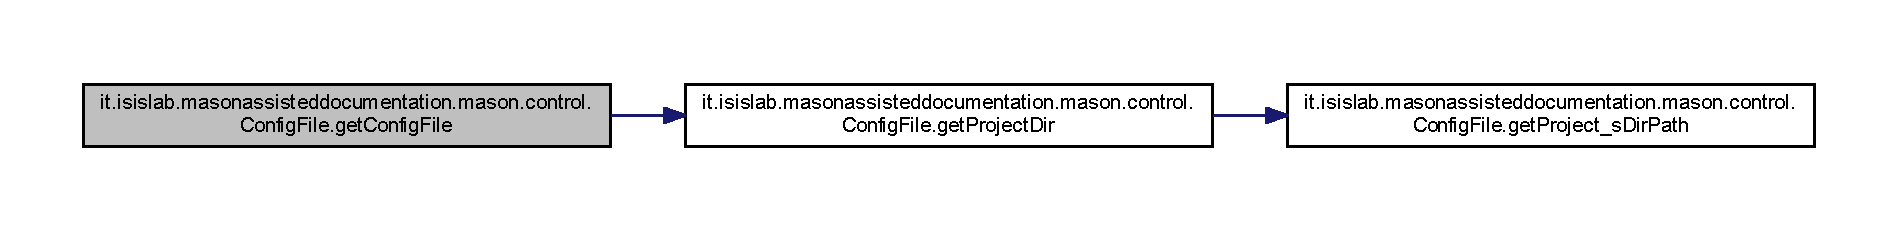
\includegraphics[width=350pt]{classit_1_1isislab_1_1masonassisteddocumentation_1_1mason_1_1control_1_1_config_file_af791ff01652e95f6385641909b805e20_cgraph}
\end{center}
\end{figure}




Here is the caller graph for this function\-:
\nopagebreak
\begin{figure}[H]
\begin{center}
\leavevmode
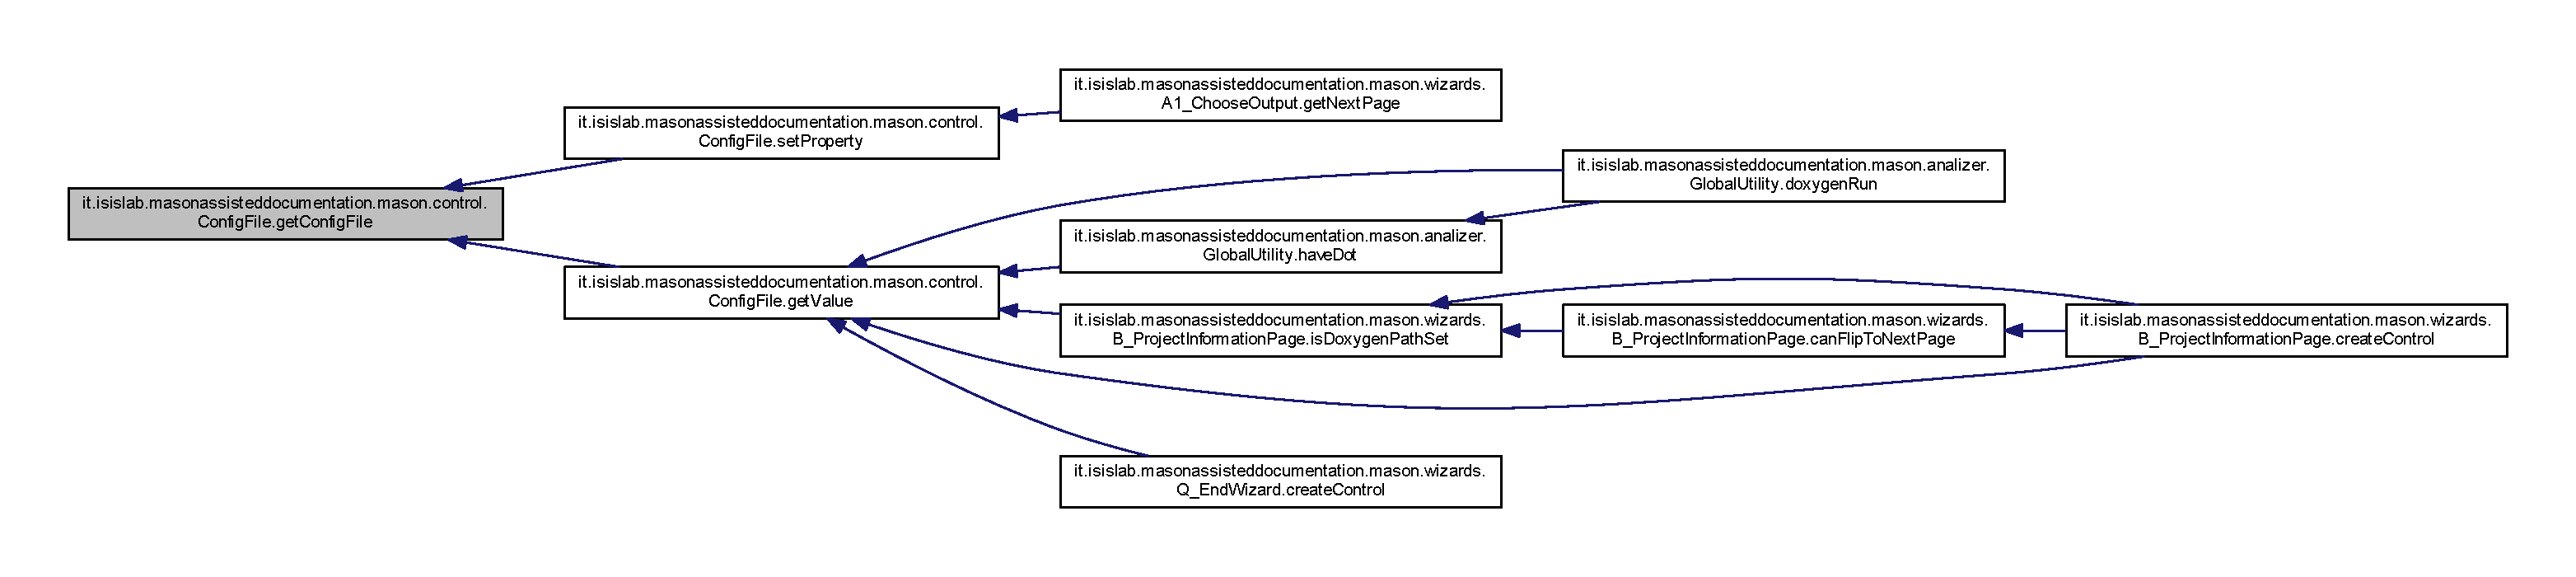
\includegraphics[width=350pt]{classit_1_1isislab_1_1masonassisteddocumentation_1_1mason_1_1control_1_1_config_file_af791ff01652e95f6385641909b805e20_icgraph}
\end{center}
\end{figure}


\hypertarget{classit_1_1isislab_1_1masonassisteddocumentation_1_1mason_1_1control_1_1_config_file_add444e913763f18b80005e5ad477c59d}{\index{it\-::isislab\-::masonassisteddocumentation\-::mason\-::control\-::\-Config\-File@{it\-::isislab\-::masonassisteddocumentation\-::mason\-::control\-::\-Config\-File}!get\-Project\-\_\-s\-Dir\-Path@{get\-Project\-\_\-s\-Dir\-Path}}
\index{get\-Project\-\_\-s\-Dir\-Path@{get\-Project\-\_\-s\-Dir\-Path}!it::isislab::masonassisteddocumentation::mason::control::ConfigFile@{it\-::isislab\-::masonassisteddocumentation\-::mason\-::control\-::\-Config\-File}}
\subsubsection[{get\-Project\-\_\-s\-Dir\-Path}]{\setlength{\rightskip}{0pt plus 5cm}static String it.\-isislab.\-masonassisteddocumentation.\-mason.\-control.\-Config\-File.\-get\-Project\-\_\-s\-Dir\-Path (
\begin{DoxyParamCaption}
{}
\end{DoxyParamCaption}
)\hspace{0.3cm}{\ttfamily [static]}}}\label{classit_1_1isislab_1_1masonassisteddocumentation_1_1mason_1_1control_1_1_config_file_add444e913763f18b80005e5ad477c59d}

\begin{DoxyCode}
29                                               \{
30         String dirPath = File.separator + \hyperlink{classit_1_1isislab_1_1masonassisteddocumentation_1_1mason_1_1control_1_1_config_file_a91a0d496b1cb5b351d2b0452fa71f763}{project\_sDirPath};
31         File project\_sDir = \textcolor{keyword}{new} File(dirPath);
32         \textcolor{keywordflow}{if} (!project\_sDir.exists())
33             \textcolor{keyword}{new} File(dirPath).mkdir();
34         log.info(\textcolor{stringliteral}{"create/get dir: "} + dirPath);
35         \textcolor{keywordflow}{return} dirPath;
36     \}
\end{DoxyCode}


Here is the caller graph for this function\-:
\nopagebreak
\begin{figure}[H]
\begin{center}
\leavevmode
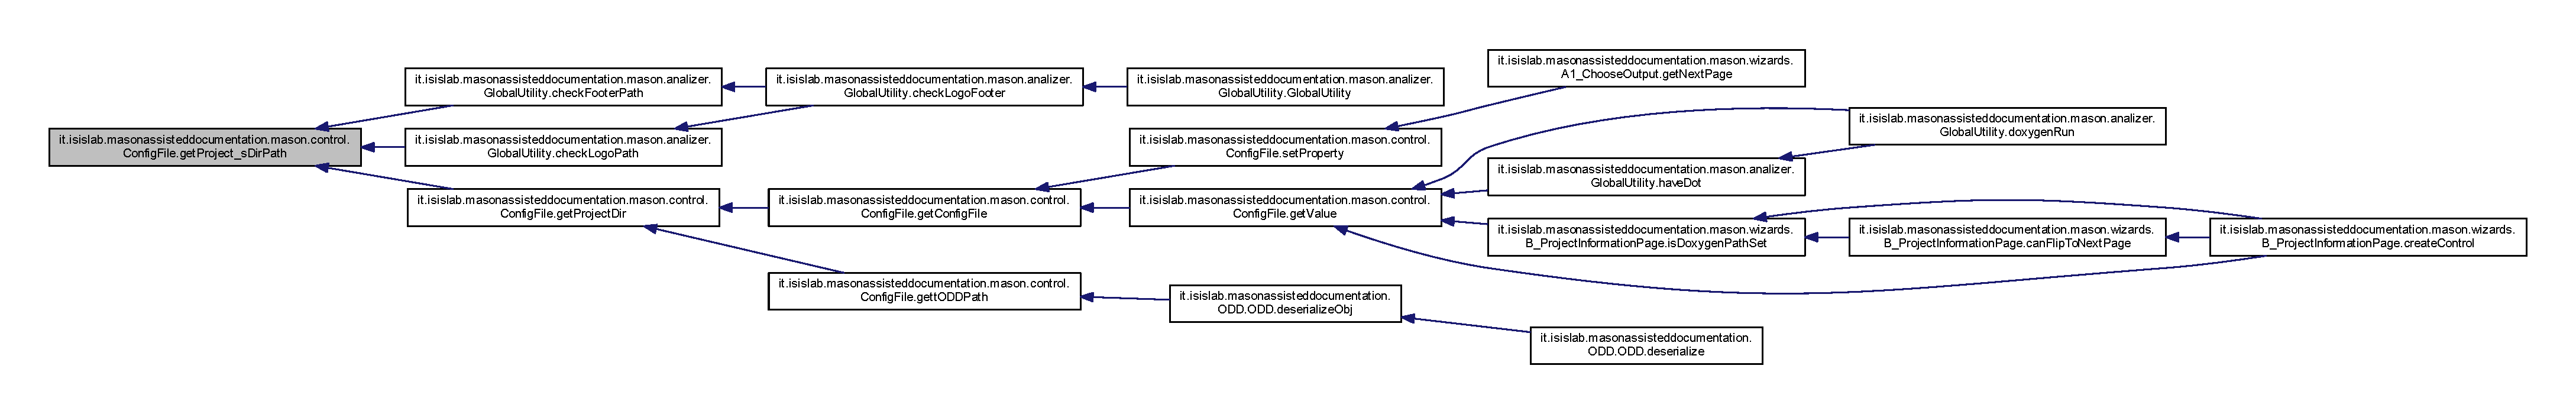
\includegraphics[width=350pt]{classit_1_1isislab_1_1masonassisteddocumentation_1_1mason_1_1control_1_1_config_file_add444e913763f18b80005e5ad477c59d_icgraph}
\end{center}
\end{figure}


\hypertarget{classit_1_1isislab_1_1masonassisteddocumentation_1_1mason_1_1control_1_1_config_file_a67bf373e54fb3ce5144d6f4fcbb48bfd}{\index{it\-::isislab\-::masonassisteddocumentation\-::mason\-::control\-::\-Config\-File@{it\-::isislab\-::masonassisteddocumentation\-::mason\-::control\-::\-Config\-File}!get\-Project\-Dir@{get\-Project\-Dir}}
\index{get\-Project\-Dir@{get\-Project\-Dir}!it::isislab::masonassisteddocumentation::mason::control::ConfigFile@{it\-::isislab\-::masonassisteddocumentation\-::mason\-::control\-::\-Config\-File}}
\subsubsection[{get\-Project\-Dir}]{\setlength{\rightskip}{0pt plus 5cm}static String it.\-isislab.\-masonassisteddocumentation.\-mason.\-control.\-Config\-File.\-get\-Project\-Dir (
\begin{DoxyParamCaption}
{}
\end{DoxyParamCaption}
)\hspace{0.3cm}{\ttfamily [static]}}}\label{classit_1_1isislab_1_1masonassisteddocumentation_1_1mason_1_1control_1_1_config_file_a67bf373e54fb3ce5144d6f4fcbb48bfd}
Return directory path for project that we are analyzing; directory will be create (if does not exist) in disk root.

\begin{DoxyReturn}{Returns}

\end{DoxyReturn}

\begin{DoxyCode}
45                                          \{
46         String dirPath = \hyperlink{classit_1_1isislab_1_1masonassisteddocumentation_1_1mason_1_1control_1_1_config_file_add444e913763f18b80005e5ad477c59d}{getProject\_sDirPath}() + File.separator + 
      \hyperlink{classit_1_1isislab_1_1masonassisteddocumentation_1_1mason_1_1control_1_1_config_file_a221de037cd407ebbe144ef1dd91b82d2}{baseDirName} + GlobalUtility.getProjectAnalizer().getProjectName();
47         \textcolor{keyword}{new} File(dirPath).mkdir();
48         log.info(\textcolor{stringliteral}{"create/get dir: "} + dirPath);
49         \textcolor{keywordflow}{return} dirPath;
50     \}
\end{DoxyCode}


Here is the call graph for this function\-:\nopagebreak
\begin{figure}[H]
\begin{center}
\leavevmode
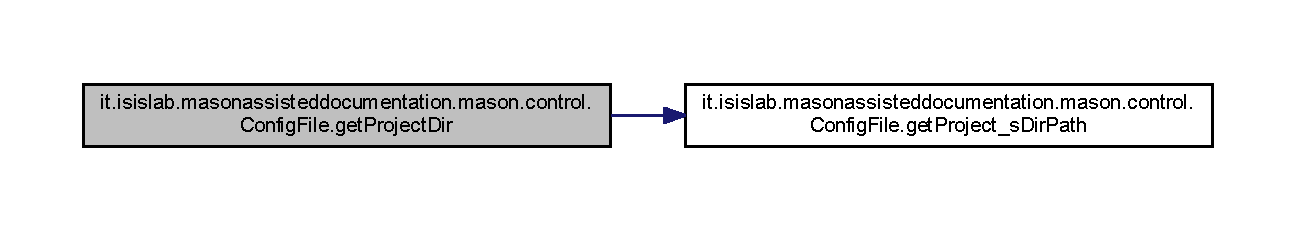
\includegraphics[width=350pt]{classit_1_1isislab_1_1masonassisteddocumentation_1_1mason_1_1control_1_1_config_file_a67bf373e54fb3ce5144d6f4fcbb48bfd_cgraph}
\end{center}
\end{figure}




Here is the caller graph for this function\-:
\nopagebreak
\begin{figure}[H]
\begin{center}
\leavevmode
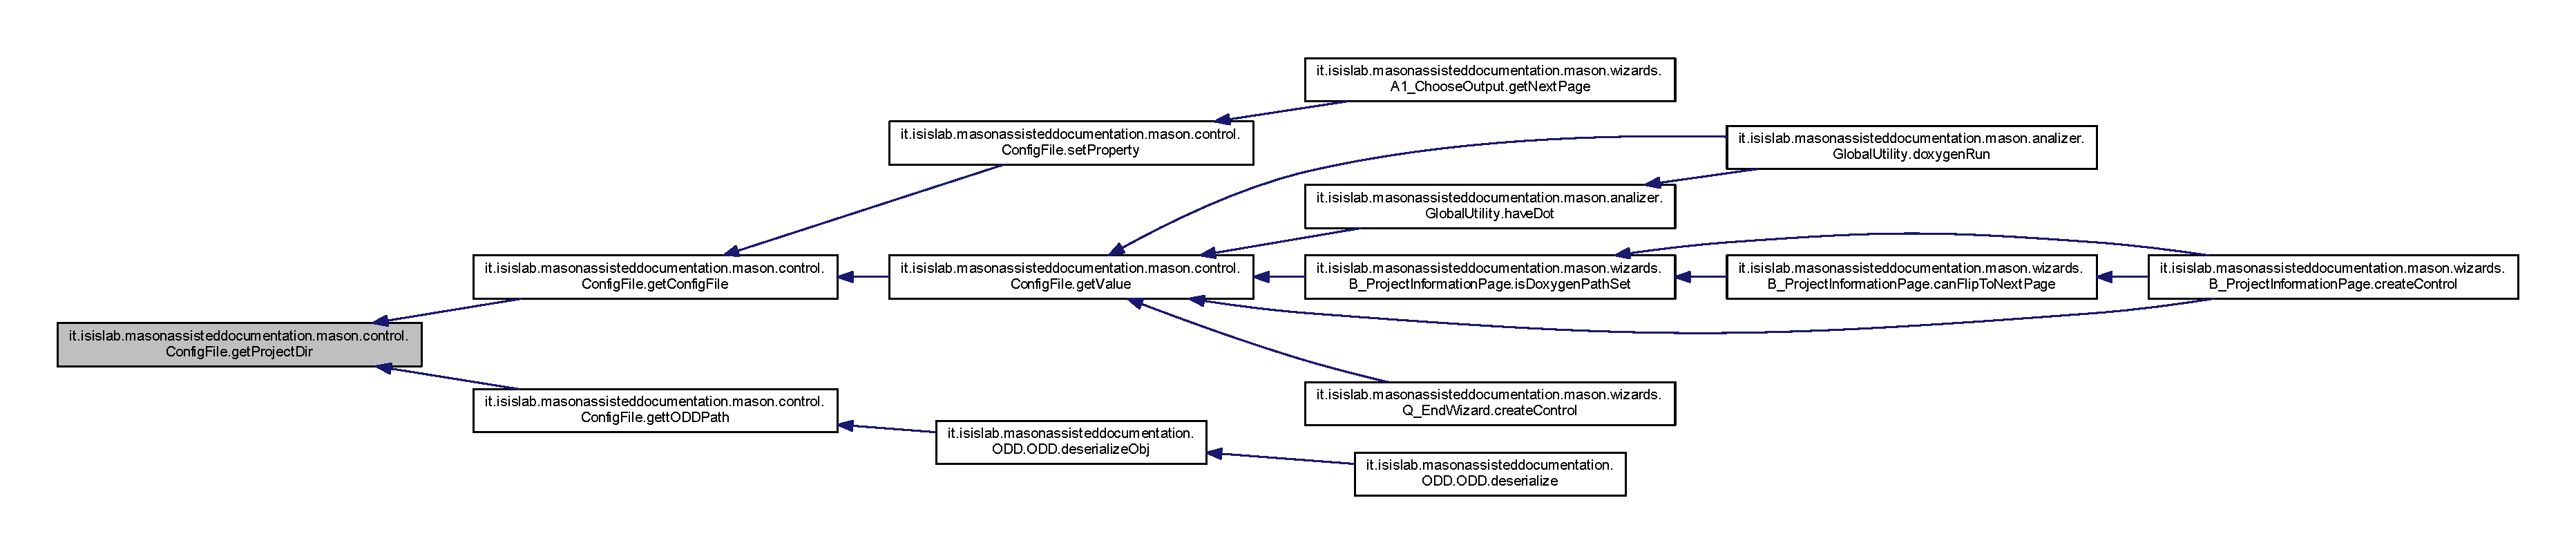
\includegraphics[width=350pt]{classit_1_1isislab_1_1masonassisteddocumentation_1_1mason_1_1control_1_1_config_file_a67bf373e54fb3ce5144d6f4fcbb48bfd_icgraph}
\end{center}
\end{figure}


\hypertarget{classit_1_1isislab_1_1masonassisteddocumentation_1_1mason_1_1control_1_1_config_file_a0bc9608fcc97bf301d3529c9ee9ae5f8}{\index{it\-::isislab\-::masonassisteddocumentation\-::mason\-::control\-::\-Config\-File@{it\-::isislab\-::masonassisteddocumentation\-::mason\-::control\-::\-Config\-File}!get\-Source\-Backup\-Dir@{get\-Source\-Backup\-Dir}}
\index{get\-Source\-Backup\-Dir@{get\-Source\-Backup\-Dir}!it::isislab::masonassisteddocumentation::mason::control::ConfigFile@{it\-::isislab\-::masonassisteddocumentation\-::mason\-::control\-::\-Config\-File}}
\subsubsection[{get\-Source\-Backup\-Dir}]{\setlength{\rightskip}{0pt plus 5cm}static String it.\-isislab.\-masonassisteddocumentation.\-mason.\-control.\-Config\-File.\-get\-Source\-Backup\-Dir (
\begin{DoxyParamCaption}
{}
\end{DoxyParamCaption}
)\hspace{0.3cm}{\ttfamily [static]}}}\label{classit_1_1isislab_1_1masonassisteddocumentation_1_1mason_1_1control_1_1_config_file_a0bc9608fcc97bf301d3529c9ee9ae5f8}
Return path of directory for code backup. In this directory will insert commented code first to remove doxygen comments. \begin{DoxyReturn}{Returns}

\end{DoxyReturn}

\begin{DoxyCode}
58                                              \{
59         String dirPath = \hyperlink{classit_1_1isislab_1_1masonassisteddocumentation_1_1mason_1_1control_1_1_config_file_add444e913763f18b80005e5ad477c59d}{getProject\_sDirPath}() + File.separator + 
      \hyperlink{classit_1_1isislab_1_1masonassisteddocumentation_1_1mason_1_1control_1_1_config_file_a221de037cd407ebbe144ef1dd91b82d2}{baseDirName} + GlobalUtility.getProjectAnalizer().getProjectName() + File.separator + \textcolor{stringliteral}{"
      BackupCodeWithComments"};
60         \textcolor{keyword}{new} File(dirPath).mkdir();
61         log.info(\textcolor{stringliteral}{"create/get dir: "} + dirPath);
62         \textcolor{keywordflow}{return} dirPath;
63     \}
\end{DoxyCode}


Here is the call graph for this function\-:
\nopagebreak
\begin{figure}[H]
\begin{center}
\leavevmode
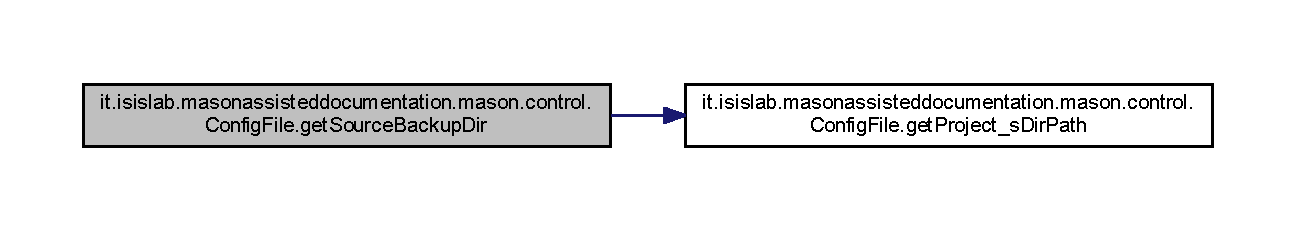
\includegraphics[width=350pt]{classit_1_1isislab_1_1masonassisteddocumentation_1_1mason_1_1control_1_1_config_file_a0bc9608fcc97bf301d3529c9ee9ae5f8_cgraph}
\end{center}
\end{figure}


\hypertarget{classit_1_1isislab_1_1masonassisteddocumentation_1_1mason_1_1control_1_1_config_file_a69e02ec967d2a3c44d590d146036d816}{\index{it\-::isislab\-::masonassisteddocumentation\-::mason\-::control\-::\-Config\-File@{it\-::isislab\-::masonassisteddocumentation\-::mason\-::control\-::\-Config\-File}!gett\-O\-D\-D\-Path@{gett\-O\-D\-D\-Path}}
\index{gett\-O\-D\-D\-Path@{gett\-O\-D\-D\-Path}!it::isislab::masonassisteddocumentation::mason::control::ConfigFile@{it\-::isislab\-::masonassisteddocumentation\-::mason\-::control\-::\-Config\-File}}
\subsubsection[{gett\-O\-D\-D\-Path}]{\setlength{\rightskip}{0pt plus 5cm}static String it.\-isislab.\-masonassisteddocumentation.\-mason.\-control.\-Config\-File.\-gett\-O\-D\-D\-Path (
\begin{DoxyParamCaption}
{}
\end{DoxyParamCaption}
)\hspace{0.3cm}{\ttfamily [static]}}}\label{classit_1_1isislab_1_1masonassisteddocumentation_1_1mason_1_1control_1_1_config_file_a69e02ec967d2a3c44d590d146036d816}

\begin{DoxyCode}
161                                        \{
162         \textcolor{keywordflow}{return} \hyperlink{classit_1_1isislab_1_1masonassisteddocumentation_1_1mason_1_1control_1_1_config_file_a67bf373e54fb3ce5144d6f4fcbb48bfd}{getProjectDir}() + File.separator;
163     \}
\end{DoxyCode}


Here is the call graph for this function\-:\nopagebreak
\begin{figure}[H]
\begin{center}
\leavevmode
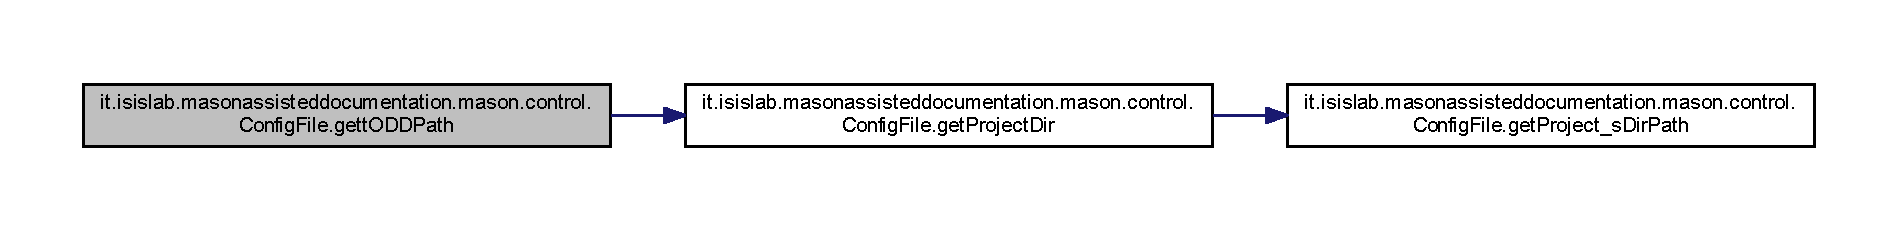
\includegraphics[width=350pt]{classit_1_1isislab_1_1masonassisteddocumentation_1_1mason_1_1control_1_1_config_file_a69e02ec967d2a3c44d590d146036d816_cgraph}
\end{center}
\end{figure}




Here is the caller graph for this function\-:\nopagebreak
\begin{figure}[H]
\begin{center}
\leavevmode
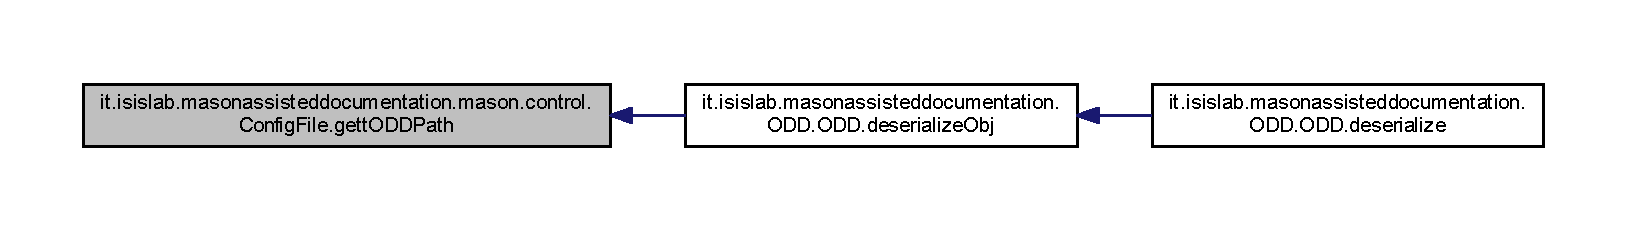
\includegraphics[width=350pt]{classit_1_1isislab_1_1masonassisteddocumentation_1_1mason_1_1control_1_1_config_file_a69e02ec967d2a3c44d590d146036d816_icgraph}
\end{center}
\end{figure}


\hypertarget{classit_1_1isislab_1_1masonassisteddocumentation_1_1mason_1_1control_1_1_config_file_abb43073f42616e4349b2fcb4e964c648}{\index{it\-::isislab\-::masonassisteddocumentation\-::mason\-::control\-::\-Config\-File@{it\-::isislab\-::masonassisteddocumentation\-::mason\-::control\-::\-Config\-File}!get\-Value@{get\-Value}}
\index{get\-Value@{get\-Value}!it::isislab::masonassisteddocumentation::mason::control::ConfigFile@{it\-::isislab\-::masonassisteddocumentation\-::mason\-::control\-::\-Config\-File}}
\subsubsection[{get\-Value}]{\setlength{\rightskip}{0pt plus 5cm}static String it.\-isislab.\-masonassisteddocumentation.\-mason.\-control.\-Config\-File.\-get\-Value (
\begin{DoxyParamCaption}
\item[{String}]{key}
\end{DoxyParamCaption}
)\hspace{0.3cm}{\ttfamily [static]}}}\label{classit_1_1isislab_1_1masonassisteddocumentation_1_1mason_1_1control_1_1_config_file_abb43073f42616e4349b2fcb4e964c648}
Return the value associated to input key


\begin{DoxyParams}{Parameters}
{\em key} & \\
\hline
\end{DoxyParams}
\begin{DoxyReturn}{Returns}

\end{DoxyReturn}

\begin{DoxyCode}
136                                               \{
137         FileInputStream fstream = null;
138         DataInputStream in = null;
139 
140         \textcolor{keywordflow}{try} \{
141             fstream = \textcolor{keyword}{new} FileInputStream(\hyperlink{classit_1_1isislab_1_1masonassisteddocumentation_1_1mason_1_1control_1_1_config_file_af791ff01652e95f6385641909b805e20}{getConfigFile}());
142             in = \textcolor{keyword}{new} DataInputStream(fstream);
143             BufferedReader br = \textcolor{keyword}{new} BufferedReader(\textcolor{keyword}{new} InputStreamReader(in));
144             String strLine;
145             \textcolor{keywordflow}{while} ((strLine = br.readLine()) != null) \{
146                 \textcolor{keywordflow}{if} (strLine.startsWith(key)) \{
147                     log.info(\textcolor{stringliteral}{"Get key: "} + key + \textcolor{stringliteral}{"; returned value: "} + strLine.split(\textcolor{stringliteral}{"="})[1]);
148                     \textcolor{keywordflow}{return} strLine.split(\textcolor{stringliteral}{"="})[1];
149                 \}
150             \}
151         \} \textcolor{keywordflow}{catch} (FileNotFoundException e) \{
152             log.severe(\textcolor{stringliteral}{"File not found: '"} + \hyperlink{classit_1_1isislab_1_1masonassisteddocumentation_1_1mason_1_1control_1_1_config_file_af791ff01652e95f6385641909b805e20}{getConfigFile}() + \textcolor{stringliteral}{"' "}
153                     + e.getMessage());
154         \} \textcolor{keywordflow}{catch} (IOException e) \{
155             log.severe(\textcolor{stringliteral}{"Error reading file: '"} + \hyperlink{classit_1_1isislab_1_1masonassisteddocumentation_1_1mason_1_1control_1_1_config_file_af791ff01652e95f6385641909b805e20}{getConfigFile}() + \textcolor{stringliteral}{"' "}
156                     + e.getMessage());
157         \}
158         \textcolor{keywordflow}{return} \textcolor{stringliteral}{""};
159     \}
\end{DoxyCode}


Here is the call graph for this function\-:\nopagebreak
\begin{figure}[H]
\begin{center}
\leavevmode
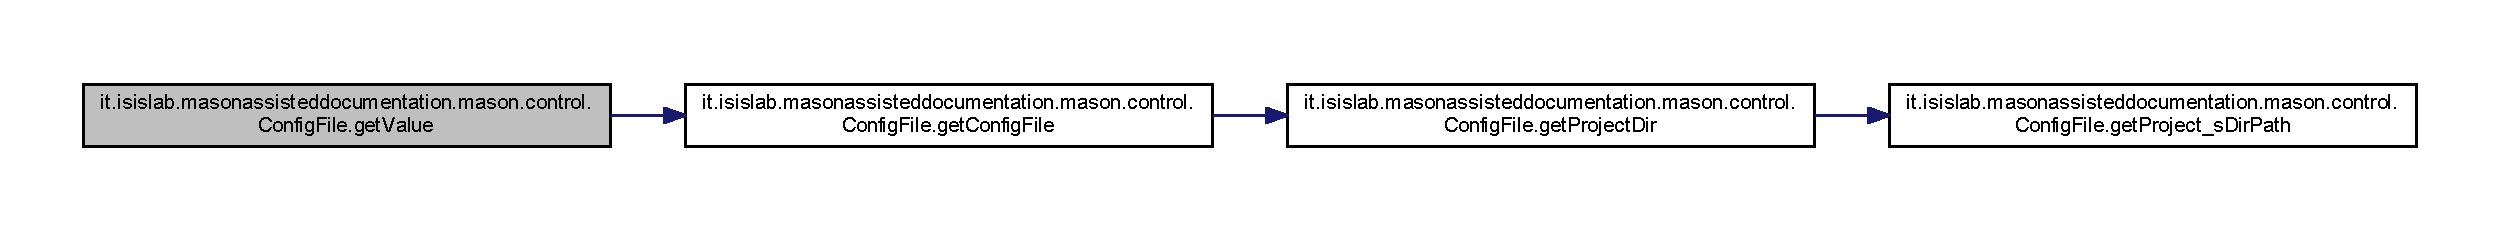
\includegraphics[width=350pt]{classit_1_1isislab_1_1masonassisteddocumentation_1_1mason_1_1control_1_1_config_file_abb43073f42616e4349b2fcb4e964c648_cgraph}
\end{center}
\end{figure}




Here is the caller graph for this function\-:
\nopagebreak
\begin{figure}[H]
\begin{center}
\leavevmode
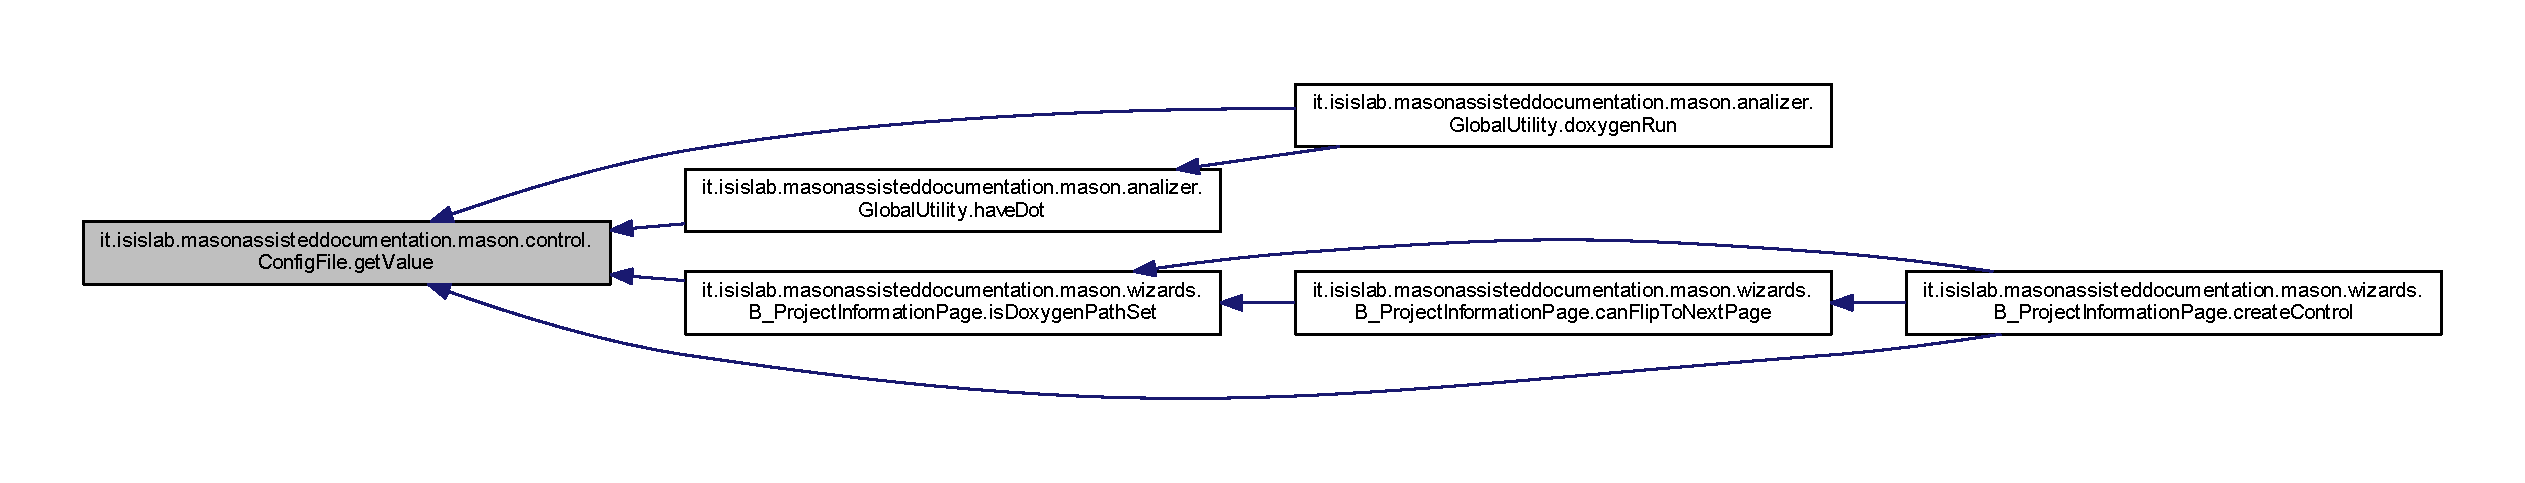
\includegraphics[width=350pt]{classit_1_1isislab_1_1masonassisteddocumentation_1_1mason_1_1control_1_1_config_file_abb43073f42616e4349b2fcb4e964c648_icgraph}
\end{center}
\end{figure}


\hypertarget{classit_1_1isislab_1_1masonassisteddocumentation_1_1mason_1_1control_1_1_config_file_ae68816366df216e1d9525047c91e77fc}{\index{it\-::isislab\-::masonassisteddocumentation\-::mason\-::control\-::\-Config\-File@{it\-::isislab\-::masonassisteddocumentation\-::mason\-::control\-::\-Config\-File}!set\-Property@{set\-Property}}
\index{set\-Property@{set\-Property}!it::isislab::masonassisteddocumentation::mason::control::ConfigFile@{it\-::isislab\-::masonassisteddocumentation\-::mason\-::control\-::\-Config\-File}}
\subsubsection[{set\-Property}]{\setlength{\rightskip}{0pt plus 5cm}static void it.\-isislab.\-masonassisteddocumentation.\-mason.\-control.\-Config\-File.\-set\-Property (
\begin{DoxyParamCaption}
\item[{String}]{key, }
\item[{String}]{value}
\end{DoxyParamCaption}
)\hspace{0.3cm}{\ttfamily [static]}}}\label{classit_1_1isislab_1_1masonassisteddocumentation_1_1mason_1_1control_1_1_config_file_ae68816366df216e1d9525047c91e77fc}
Set the key to value in \hyperlink{classit_1_1isislab_1_1masonassisteddocumentation_1_1mason_1_1control_1_1_config_file}{Config\-File} pointed by config\-File\-Path


\begin{DoxyParams}{Parameters}
{\em key} & \\
\hline
{\em value} & \\
\hline
\end{DoxyParams}

\begin{DoxyCode}
85                                                              \{
86         FileInputStream fstream = null;
87         DataInputStream in = null;
88         BufferedWriter out = null;
89         \textcolor{keywordtype}{boolean} propertySet = \textcolor{keyword}{false};
90 
91         \textcolor{keywordflow}{try} \{
92             fstream = \textcolor{keyword}{new} FileInputStream(\hyperlink{classit_1_1isislab_1_1masonassisteddocumentation_1_1mason_1_1control_1_1_config_file_af791ff01652e95f6385641909b805e20}{getConfigFile}());
93             in = \textcolor{keyword}{new} DataInputStream(fstream);
94             BufferedReader br = \textcolor{keyword}{new} BufferedReader(\textcolor{keyword}{new} InputStreamReader(in));
95             String strLine;
96             StringBuilder fileContent = \textcolor{keyword}{new} StringBuilder();
97 
98             \textcolor{keywordflow}{while} ((strLine = br.readLine()) != null) \{
99                 \textcolor{keywordflow}{if} (strLine.startsWith(key)) \{
100                     fileContent.append(key + \textcolor{stringliteral}{"="} + value
101                             + System.getProperty(\textcolor{stringliteral}{"line.separator"}));
102                     propertySet = \textcolor{keyword}{true};
103                 \} \textcolor{keywordflow}{else} \{
104                     fileContent.append(strLine);
105                     fileContent.append(System.getProperty(\textcolor{stringliteral}{"line.separator"}));
106                 \}
107             \}
108             \textcolor{keywordflow}{if} (!propertySet) \{
109                 fileContent.append(key + \textcolor{stringliteral}{"="} + value);
110             \}
111 
112             FileWriter fstreamWrite = \textcolor{keyword}{new} FileWriter(\hyperlink{classit_1_1isislab_1_1masonassisteddocumentation_1_1mason_1_1control_1_1_config_file_af791ff01652e95f6385641909b805e20}{getConfigFile}());
113             out = \textcolor{keyword}{new} BufferedWriter(fstreamWrite);
114             out.write(fileContent.toString());
115         \} \textcolor{keywordflow}{catch} (Exception e) \{
116             e.printStackTrace();
117         \} \textcolor{keywordflow}{finally} \{
118             \textcolor{keywordflow}{try} \{
119                 fstream.close();
120                 out.flush();
121                 out.close();
122                 in.close();
123             \} \textcolor{keywordflow}{catch} (IOException e) \{
124                 e.printStackTrace();
125             \}
126         \}
127         log.info(\textcolor{stringliteral}{"Set key: "} + key + \textcolor{stringliteral}{" to value: "} + value);
128     \}
\end{DoxyCode}


Here is the call graph for this function\-:\nopagebreak
\begin{figure}[H]
\begin{center}
\leavevmode
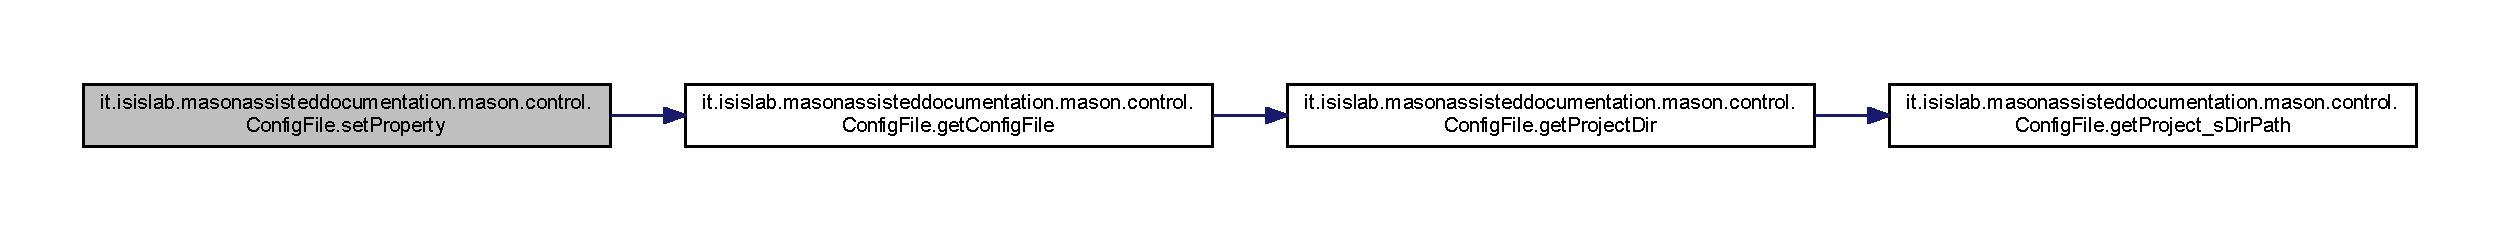
\includegraphics[width=350pt]{classit_1_1isislab_1_1masonassisteddocumentation_1_1mason_1_1control_1_1_config_file_ae68816366df216e1d9525047c91e77fc_cgraph}
\end{center}
\end{figure}




Here is the caller graph for this function\-:\nopagebreak
\begin{figure}[H]
\begin{center}
\leavevmode
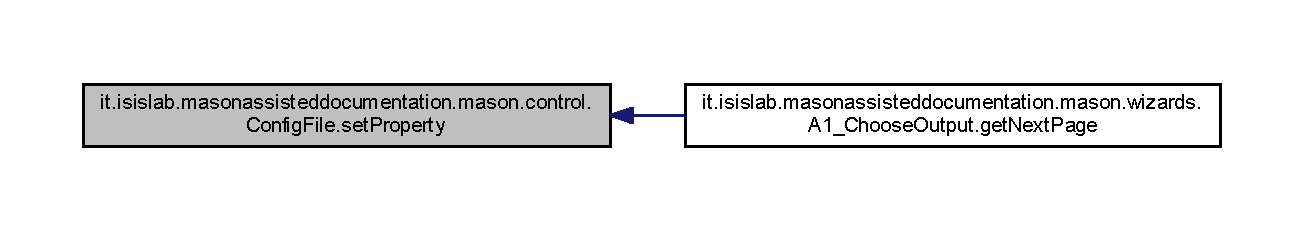
\includegraphics[width=350pt]{classit_1_1isislab_1_1masonassisteddocumentation_1_1mason_1_1control_1_1_config_file_ae68816366df216e1d9525047c91e77fc_icgraph}
\end{center}
\end{figure}




\subsection{Member Data Documentation}
\hypertarget{classit_1_1isislab_1_1masonassisteddocumentation_1_1mason_1_1control_1_1_config_file_a221de037cd407ebbe144ef1dd91b82d2}{\index{it\-::isislab\-::masonassisteddocumentation\-::mason\-::control\-::\-Config\-File@{it\-::isislab\-::masonassisteddocumentation\-::mason\-::control\-::\-Config\-File}!base\-Dir\-Name@{base\-Dir\-Name}}
\index{base\-Dir\-Name@{base\-Dir\-Name}!it::isislab::masonassisteddocumentation::mason::control::ConfigFile@{it\-::isislab\-::masonassisteddocumentation\-::mason\-::control\-::\-Config\-File}}
\subsubsection[{base\-Dir\-Name}]{\setlength{\rightskip}{0pt plus 5cm}String it.\-isislab.\-masonassisteddocumentation.\-mason.\-control.\-Config\-File.\-base\-Dir\-Name = \char`\"{}M\-A\-D\-\_\-\char`\"{}\hspace{0.3cm}{\ttfamily [static]}, {\ttfamily [private]}}}\label{classit_1_1isislab_1_1masonassisteddocumentation_1_1mason_1_1control_1_1_config_file_a221de037cd407ebbe144ef1dd91b82d2}
\hypertarget{classit_1_1isislab_1_1masonassisteddocumentation_1_1mason_1_1control_1_1_config_file_abcfdfd0e472ce37556509fbe6ec06a10}{\index{it\-::isislab\-::masonassisteddocumentation\-::mason\-::control\-::\-Config\-File@{it\-::isislab\-::masonassisteddocumentation\-::mason\-::control\-::\-Config\-File}!config\-File\-Name@{config\-File\-Name}}
\index{config\-File\-Name@{config\-File\-Name}!it::isislab::masonassisteddocumentation::mason::control::ConfigFile@{it\-::isislab\-::masonassisteddocumentation\-::mason\-::control\-::\-Config\-File}}
\subsubsection[{config\-File\-Name}]{\setlength{\rightskip}{0pt plus 5cm}String it.\-isislab.\-masonassisteddocumentation.\-mason.\-control.\-Config\-File.\-config\-File\-Name = \char`\"{}M\-A\-D\-\_\-config.\-dat\char`\"{}\hspace{0.3cm}{\ttfamily [static]}, {\ttfamily [private]}}}\label{classit_1_1isislab_1_1masonassisteddocumentation_1_1mason_1_1control_1_1_config_file_abcfdfd0e472ce37556509fbe6ec06a10}
\hypertarget{classit_1_1isislab_1_1masonassisteddocumentation_1_1mason_1_1control_1_1_config_file_a233d40b4ec2b6609570825bedaa9f6e5}{\index{it\-::isislab\-::masonassisteddocumentation\-::mason\-::control\-::\-Config\-File@{it\-::isislab\-::masonassisteddocumentation\-::mason\-::control\-::\-Config\-File}!log@{log}}
\index{log@{log}!it::isislab::masonassisteddocumentation::mason::control::ConfigFile@{it\-::isislab\-::masonassisteddocumentation\-::mason\-::control\-::\-Config\-File}}
\subsubsection[{log}]{\setlength{\rightskip}{0pt plus 5cm}Logger it.\-isislab.\-masonassisteddocumentation.\-mason.\-control.\-Config\-File.\-log = Logger.\-get\-Logger(\char`\"{}global\char`\"{})\hspace{0.3cm}{\ttfamily [static]}, {\ttfamily [private]}}}\label{classit_1_1isislab_1_1masonassisteddocumentation_1_1mason_1_1control_1_1_config_file_a233d40b4ec2b6609570825bedaa9f6e5}
\hypertarget{classit_1_1isislab_1_1masonassisteddocumentation_1_1mason_1_1control_1_1_config_file_a91a0d496b1cb5b351d2b0452fa71f763}{\index{it\-::isislab\-::masonassisteddocumentation\-::mason\-::control\-::\-Config\-File@{it\-::isislab\-::masonassisteddocumentation\-::mason\-::control\-::\-Config\-File}!project\-\_\-s\-Dir\-Path@{project\-\_\-s\-Dir\-Path}}
\index{project\-\_\-s\-Dir\-Path@{project\-\_\-s\-Dir\-Path}!it::isislab::masonassisteddocumentation::mason::control::ConfigFile@{it\-::isislab\-::masonassisteddocumentation\-::mason\-::control\-::\-Config\-File}}
\subsubsection[{project\-\_\-s\-Dir\-Path}]{\setlength{\rightskip}{0pt plus 5cm}String it.\-isislab.\-masonassisteddocumentation.\-mason.\-control.\-Config\-File.\-project\-\_\-s\-Dir\-Path = \char`\"{}M\-A\-D(Mason-\/Assisted-\/Documentation)\char`\"{}\hspace{0.3cm}{\ttfamily [static]}, {\ttfamily [private]}}}\label{classit_1_1isislab_1_1masonassisteddocumentation_1_1mason_1_1control_1_1_config_file_a91a0d496b1cb5b351d2b0452fa71f763}


The documentation for this class was generated from the following file\-:\begin{DoxyCompactItemize}
\item 
src/it/isislab/masonassisteddocumentation/mason/control/\hyperlink{_config_file_8java}{Config\-File.\-java}\end{DoxyCompactItemize}

\hypertarget{classit_1_1isislab_1_1masonassisteddocumentation_1_1mason_1_1wizards_1_1_d___agent_description_page}{\section{it.\-isislab.\-masonassisteddocumentation.\-mason.\-wizards.\-D\-\_\-\-Agent\-Description\-Page Class Reference}
\label{classit_1_1isislab_1_1masonassisteddocumentation_1_1mason_1_1wizards_1_1_d___agent_description_page}\index{it.\-isislab.\-masonassisteddocumentation.\-mason.\-wizards.\-D\-\_\-\-Agent\-Description\-Page@{it.\-isislab.\-masonassisteddocumentation.\-mason.\-wizards.\-D\-\_\-\-Agent\-Description\-Page}}
}


Inheritance diagram for it.\-isislab.\-masonassisteddocumentation.\-mason.\-wizards.\-D\-\_\-\-Agent\-Description\-Page\-:\nopagebreak
\begin{figure}[H]
\begin{center}
\leavevmode
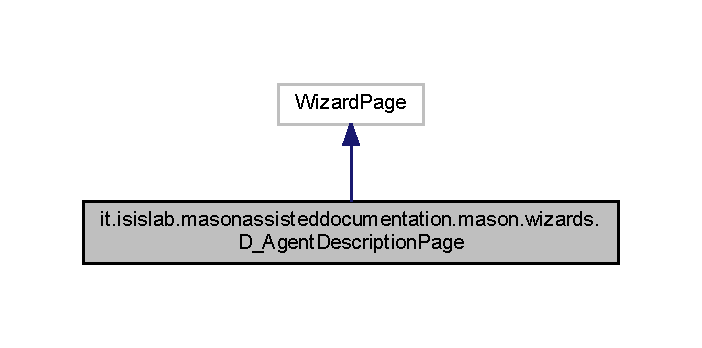
\includegraphics[width=337pt]{classit_1_1isislab_1_1masonassisteddocumentation_1_1mason_1_1wizards_1_1_d___agent_description_page__inherit__graph}
\end{center}
\end{figure}


Collaboration diagram for it.\-isislab.\-masonassisteddocumentation.\-mason.\-wizards.\-D\-\_\-\-Agent\-Description\-Page\-:\nopagebreak
\begin{figure}[H]
\begin{center}
\leavevmode
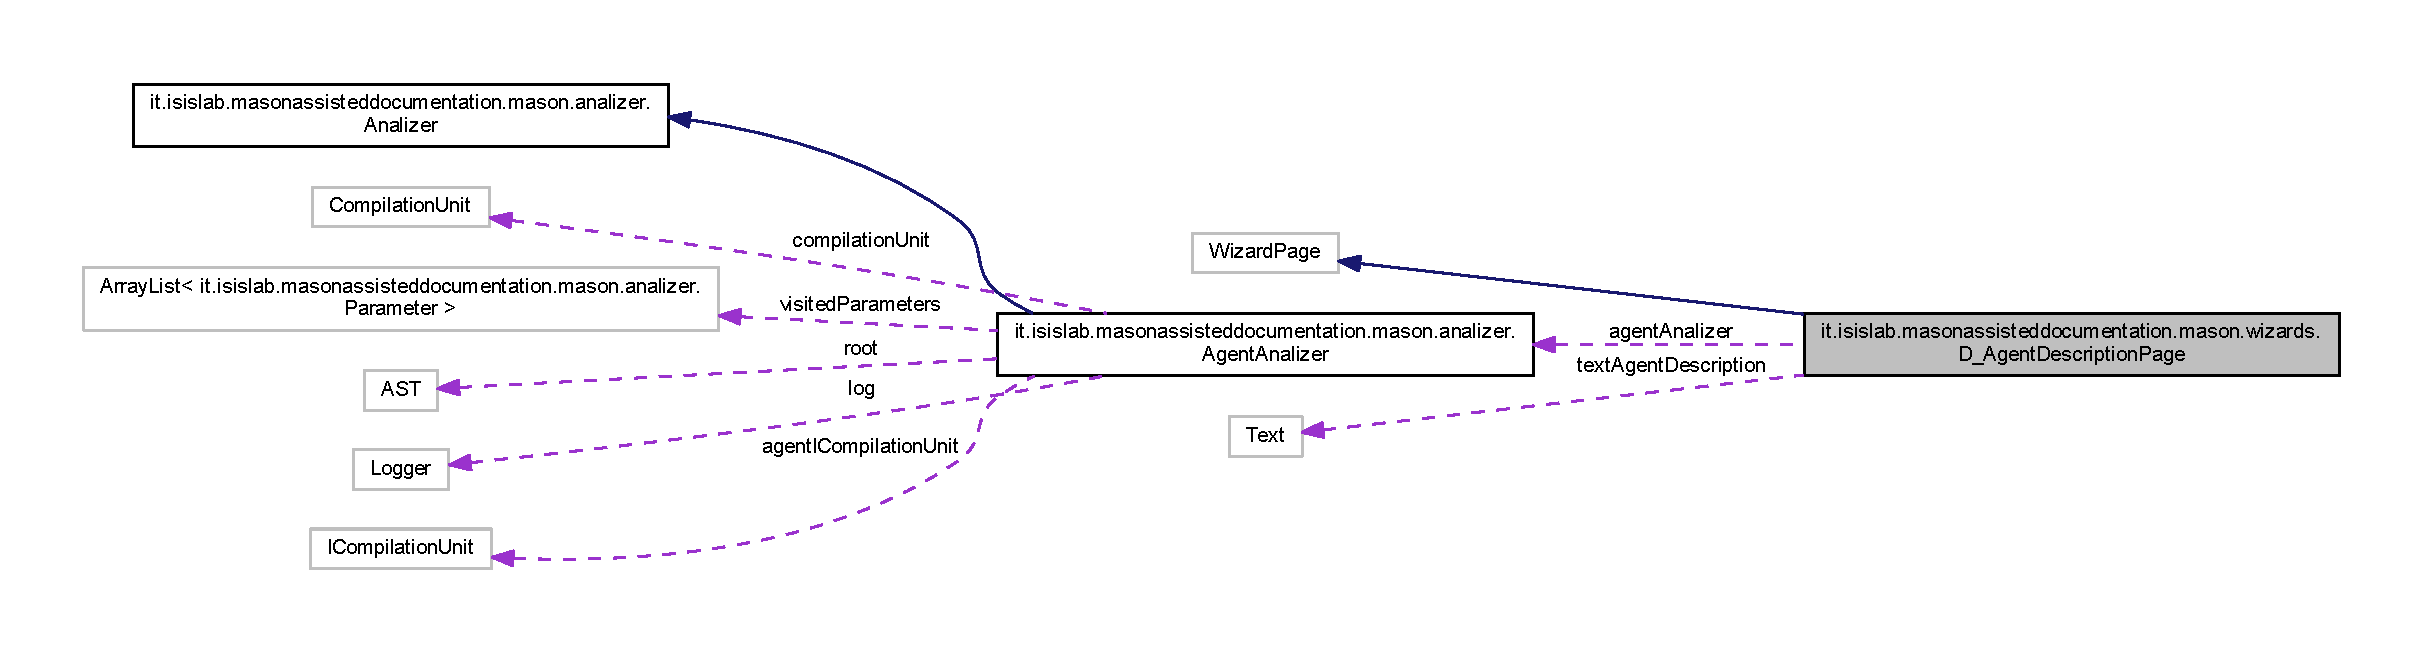
\includegraphics[width=350pt]{classit_1_1isislab_1_1masonassisteddocumentation_1_1mason_1_1wizards_1_1_d___agent_description_page__coll__graph}
\end{center}
\end{figure}
\subsection*{Public Member Functions}
\begin{DoxyCompactItemize}
\item 
\hyperlink{classit_1_1isislab_1_1masonassisteddocumentation_1_1mason_1_1wizards_1_1_d___agent_description_page_aee37d48e42e4d6f95404e42ecfd04e6d}{D\-\_\-\-Agent\-Description\-Page} ()
\item 
void \hyperlink{classit_1_1isislab_1_1masonassisteddocumentation_1_1mason_1_1wizards_1_1_d___agent_description_page_aff878d7cd601edf044658e6a06b389db}{create\-Control} (Composite parent)
\item 
boolean \hyperlink{classit_1_1isislab_1_1masonassisteddocumentation_1_1mason_1_1wizards_1_1_d___agent_description_page_a4cd29961ae4355329be27bdeb8185f15}{can\-Flip\-To\-Next\-Page} ()
\item 
I\-Wizard\-Page \hyperlink{classit_1_1isislab_1_1masonassisteddocumentation_1_1mason_1_1wizards_1_1_d___agent_description_page_acd32a9211894d81e238f54607d7b3f73}{get\-Next\-Page} ()
\end{DoxyCompactItemize}
\subsection*{Private Member Functions}
\begin{DoxyCompactItemize}
\item 
void \hyperlink{classit_1_1isislab_1_1masonassisteddocumentation_1_1mason_1_1wizards_1_1_d___agent_description_page_a0a7d91afd5148a932706e2b5c5a97b9f}{get\-Old\-Information} ()
\end{DoxyCompactItemize}
\subsection*{Private Attributes}
\begin{DoxyCompactItemize}
\item 
\hyperlink{classit_1_1isislab_1_1masonassisteddocumentation_1_1mason_1_1analizer_1_1_agent_analizer}{Agent\-Analizer} \hyperlink{classit_1_1isislab_1_1masonassisteddocumentation_1_1mason_1_1wizards_1_1_d___agent_description_page_a3551237b74a669c361623caa219af9d7}{agent\-Analizer}
\item 
Text \hyperlink{classit_1_1isislab_1_1masonassisteddocumentation_1_1mason_1_1wizards_1_1_d___agent_description_page_a36dfef5219d3c9d56facf7345020ee82}{text\-Agent\-Description}
\end{DoxyCompactItemize}
\subsection*{Static Private Attributes}
\begin{DoxyCompactItemize}
\item 
static String \hyperlink{classit_1_1isislab_1_1masonassisteddocumentation_1_1mason_1_1wizards_1_1_d___agent_description_page_a28540e2ea308e26ef8e80ba9d4848443}{page\-Description}
\end{DoxyCompactItemize}


\subsection{Detailed Description}
\begin{DoxyAuthor}{Author}
Romano Simone 0512101343 This page show agent description. 
\end{DoxyAuthor}


\subsection{Constructor \& Destructor Documentation}
\hypertarget{classit_1_1isislab_1_1masonassisteddocumentation_1_1mason_1_1wizards_1_1_d___agent_description_page_aee37d48e42e4d6f95404e42ecfd04e6d}{\index{it\-::isislab\-::masonassisteddocumentation\-::mason\-::wizards\-::\-D\-\_\-\-Agent\-Description\-Page@{it\-::isislab\-::masonassisteddocumentation\-::mason\-::wizards\-::\-D\-\_\-\-Agent\-Description\-Page}!D\-\_\-\-Agent\-Description\-Page@{D\-\_\-\-Agent\-Description\-Page}}
\index{D\-\_\-\-Agent\-Description\-Page@{D\-\_\-\-Agent\-Description\-Page}!it::isislab::masonassisteddocumentation::mason::wizards::D_AgentDescriptionPage@{it\-::isislab\-::masonassisteddocumentation\-::mason\-::wizards\-::\-D\-\_\-\-Agent\-Description\-Page}}
\subsubsection[{D\-\_\-\-Agent\-Description\-Page}]{\setlength{\rightskip}{0pt plus 5cm}it.\-isislab.\-masonassisteddocumentation.\-mason.\-wizards.\-D\-\_\-\-Agent\-Description\-Page.\-D\-\_\-\-Agent\-Description\-Page (
\begin{DoxyParamCaption}
{}
\end{DoxyParamCaption}
)}}\label{classit_1_1isislab_1_1masonassisteddocumentation_1_1mason_1_1wizards_1_1_d___agent_description_page_aee37d48e42e4d6f95404e42ecfd04e6d}
Constructor for Agent\-Description\-Page. 
\begin{DoxyParams}{Parameters}
{\em java\-Project} & \\
\hline
\end{DoxyParams}

\begin{DoxyCode}
35                                     \{
36         super(\textcolor{stringliteral}{"wizardPage"});
37         \hyperlink{classit_1_1isislab_1_1masonassisteddocumentation_1_1mason_1_1wizards_1_1_d___agent_description_page_a3551237b74a669c361623caa219af9d7}{agentAnalizer} = GlobalUtility.getAgentAnalizer();
38         setTitle(\textcolor{stringliteral}{"2/7 - Entities, state variables, and scales\(\backslash\)n"} + \hyperlink{classit_1_1isislab_1_1masonassisteddocumentation_1_1mason_1_1wizards_1_1_d___agent_description_page_a3551237b74a669c361623caa219af9d7}{agentAnalizer}.
      \hyperlink{classit_1_1isislab_1_1masonassisteddocumentation_1_1mason_1_1analizer_1_1_agent_analizer_a94492199c5e4873a07a2a46d15617937}{getClassName}());
39         setDescription(\hyperlink{classit_1_1isislab_1_1masonassisteddocumentation_1_1mason_1_1wizards_1_1_d___agent_description_page_a28540e2ea308e26ef8e80ba9d4848443}{pageDescription});
40     \}
\end{DoxyCode}


Here is the call graph for this function\-:\nopagebreak
\begin{figure}[H]
\begin{center}
\leavevmode
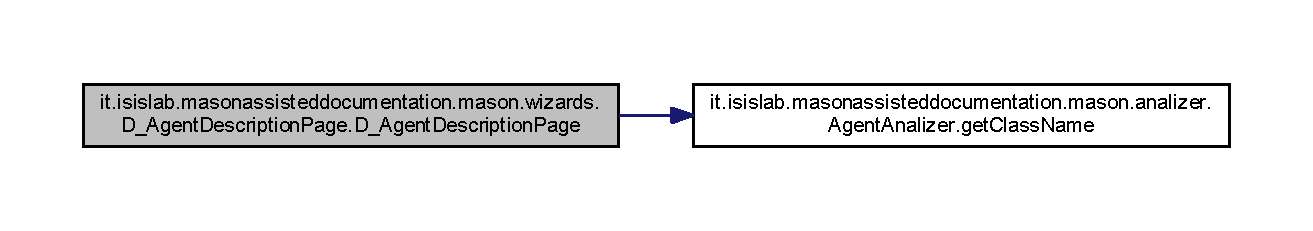
\includegraphics[width=350pt]{classit_1_1isislab_1_1masonassisteddocumentation_1_1mason_1_1wizards_1_1_d___agent_description_page_aee37d48e42e4d6f95404e42ecfd04e6d_cgraph}
\end{center}
\end{figure}




\subsection{Member Function Documentation}
\hypertarget{classit_1_1isislab_1_1masonassisteddocumentation_1_1mason_1_1wizards_1_1_d___agent_description_page_a4cd29961ae4355329be27bdeb8185f15}{\index{it\-::isislab\-::masonassisteddocumentation\-::mason\-::wizards\-::\-D\-\_\-\-Agent\-Description\-Page@{it\-::isislab\-::masonassisteddocumentation\-::mason\-::wizards\-::\-D\-\_\-\-Agent\-Description\-Page}!can\-Flip\-To\-Next\-Page@{can\-Flip\-To\-Next\-Page}}
\index{can\-Flip\-To\-Next\-Page@{can\-Flip\-To\-Next\-Page}!it::isislab::masonassisteddocumentation::mason::wizards::D_AgentDescriptionPage@{it\-::isislab\-::masonassisteddocumentation\-::mason\-::wizards\-::\-D\-\_\-\-Agent\-Description\-Page}}
\subsubsection[{can\-Flip\-To\-Next\-Page}]{\setlength{\rightskip}{0pt plus 5cm}boolean it.\-isislab.\-masonassisteddocumentation.\-mason.\-wizards.\-D\-\_\-\-Agent\-Description\-Page.\-can\-Flip\-To\-Next\-Page (
\begin{DoxyParamCaption}
{}
\end{DoxyParamCaption}
)}}\label{classit_1_1isislab_1_1masonassisteddocumentation_1_1mason_1_1wizards_1_1_d___agent_description_page_a4cd29961ae4355329be27bdeb8185f15}

\begin{DoxyCode}
71                                        \{
72         \textcolor{keywordflow}{return} \textcolor{keyword}{true};
73     \}
\end{DoxyCode}
\hypertarget{classit_1_1isislab_1_1masonassisteddocumentation_1_1mason_1_1wizards_1_1_d___agent_description_page_aff878d7cd601edf044658e6a06b389db}{\index{it\-::isislab\-::masonassisteddocumentation\-::mason\-::wizards\-::\-D\-\_\-\-Agent\-Description\-Page@{it\-::isislab\-::masonassisteddocumentation\-::mason\-::wizards\-::\-D\-\_\-\-Agent\-Description\-Page}!create\-Control@{create\-Control}}
\index{create\-Control@{create\-Control}!it::isislab::masonassisteddocumentation::mason::wizards::D_AgentDescriptionPage@{it\-::isislab\-::masonassisteddocumentation\-::mason\-::wizards\-::\-D\-\_\-\-Agent\-Description\-Page}}
\subsubsection[{create\-Control}]{\setlength{\rightskip}{0pt plus 5cm}void it.\-isislab.\-masonassisteddocumentation.\-mason.\-wizards.\-D\-\_\-\-Agent\-Description\-Page.\-create\-Control (
\begin{DoxyParamCaption}
\item[{Composite}]{parent}
\end{DoxyParamCaption}
)}}\label{classit_1_1isislab_1_1masonassisteddocumentation_1_1mason_1_1wizards_1_1_d___agent_description_page_aff878d7cd601edf044658e6a06b389db}

\begin{DoxyCode}
42                                                 \{
43         Composite container = \textcolor{keyword}{new} Composite(parent, SWT.NULL);
44         setControl(container);
45         container.setLayout(\textcolor{keyword}{new} GridLayout(1,\textcolor{keyword}{true}));
46         
47         Label lblAgentDefinition = \textcolor{keyword}{new} Label(container, SWT.NONE);
48         GridData gd\_lblAgentDefinition = \textcolor{keyword}{new} GridData(SWT.CENTER, SWT.CENTER, \textcolor{keyword}{false}, \textcolor{keyword}{false}, 1, 1);
49         gd\_lblAgentDefinition.widthHint = 567;
50         lblAgentDefinition.setLayoutData(gd\_lblAgentDefinition);
51         lblAgentDefinition.setText(\textcolor{stringliteral}{"Description for entities: "} + agentAnalizer.getClassName());
52 
53         \hyperlink{classit_1_1isislab_1_1masonassisteddocumentation_1_1mason_1_1wizards_1_1_d___agent_description_page_a36dfef5219d3c9d56facf7345020ee82}{textAgentDescription} = \textcolor{keyword}{new} Text(container, SWT.BORDER | SWT.MULTI);
54         GridData gd\_text = \textcolor{keyword}{new} GridData(SWT.FILL, SWT.CENTER, \textcolor{keyword}{true}, \textcolor{keyword}{false}, 1, 1);
55         gd\_text.heightHint = 93;
56         textAgentDescription.setLayoutData(gd\_text);
57 
58         
59         \hyperlink{classit_1_1isislab_1_1masonassisteddocumentation_1_1mason_1_1wizards_1_1_d___agent_description_page_a0a7d91afd5148a932706e2b5c5a97b9f}{getOldInformation}();
60         
61     \}
\end{DoxyCode}


Here is the call graph for this function\-:\nopagebreak
\begin{figure}[H]
\begin{center}
\leavevmode
\includegraphics[width=350pt]{classit_1_1isislab_1_1masonassisteddocumentation_1_1mason_1_1wizards_1_1_d___agent_description_page_aff878d7cd601edf044658e6a06b389db_cgraph}
\end{center}
\end{figure}


\hypertarget{classit_1_1isislab_1_1masonassisteddocumentation_1_1mason_1_1wizards_1_1_d___agent_description_page_acd32a9211894d81e238f54607d7b3f73}{\index{it\-::isislab\-::masonassisteddocumentation\-::mason\-::wizards\-::\-D\-\_\-\-Agent\-Description\-Page@{it\-::isislab\-::masonassisteddocumentation\-::mason\-::wizards\-::\-D\-\_\-\-Agent\-Description\-Page}!get\-Next\-Page@{get\-Next\-Page}}
\index{get\-Next\-Page@{get\-Next\-Page}!it::isislab::masonassisteddocumentation::mason::wizards::D_AgentDescriptionPage@{it\-::isislab\-::masonassisteddocumentation\-::mason\-::wizards\-::\-D\-\_\-\-Agent\-Description\-Page}}
\subsubsection[{get\-Next\-Page}]{\setlength{\rightskip}{0pt plus 5cm}I\-Wizard\-Page it.\-isislab.\-masonassisteddocumentation.\-mason.\-wizards.\-D\-\_\-\-Agent\-Description\-Page.\-get\-Next\-Page (
\begin{DoxyParamCaption}
{}
\end{DoxyParamCaption}
)}}\label{classit_1_1isislab_1_1masonassisteddocumentation_1_1mason_1_1wizards_1_1_d___agent_description_page_acd32a9211894d81e238f54607d7b3f73}
Add this agent to Entities list (entities represent the Entites of \hyperlink{namespaceit_1_1isislab_1_1masonassisteddocumentation_1_1_o_d_d}{O\-D\-D} protocol -\/ section 2) 
\begin{DoxyParams}{Parameters}
{\em agent\-Analizer} & \\
\hline
\end{DoxyParams}

\begin{DoxyCode}
75                                     \{ 
76         \textcolor{comment}{//store new autogenerated information}
77         agentAnalizer.setClassDescription(textAgentDescription.getText());
83         ODD.addEntity(\textcolor{keyword}{new} Entity(\hyperlink{classit_1_1isislab_1_1masonassisteddocumentation_1_1mason_1_1wizards_1_1_d___agent_description_page_a3551237b74a669c361623caa219af9d7}{agentAnalizer}.\hyperlink{classit_1_1isislab_1_1masonassisteddocumentation_1_1mason_1_1analizer_1_1_agent_analizer_a94492199c5e4873a07a2a46d15617937}{getClassName}(), 
      textAgentDescription.getText()));   
84         \textcolor{keywordflow}{if} (\hyperlink{classit_1_1isislab_1_1masonassisteddocumentation_1_1mason_1_1wizards_1_1_d___agent_description_page_a3551237b74a669c361623caa219af9d7}{agentAnalizer}.\hyperlink{classit_1_1isislab_1_1masonassisteddocumentation_1_1mason_1_1analizer_1_1_agent_analizer_a351c38491d7f706177c4c76478cabd6d}{getPositionsParameter}().size() != 0)\{
85             E\_AgentPositionPage nextPage = \textcolor{keyword}{new} E\_AgentPositionPage();
86             ((MASONDocumentationWizard) super.getWizard()).addPage(nextPage); 
87             \textcolor{keywordflow}{return} nextPage; 
88         \}
89         \textcolor{keywordflow}{else} \textcolor{keywordflow}{if} (\hyperlink{classit_1_1isislab_1_1masonassisteddocumentation_1_1mason_1_1wizards_1_1_d___agent_description_page_a3551237b74a669c361623caa219af9d7}{agentAnalizer}.\hyperlink{classit_1_1isislab_1_1masonassisteddocumentation_1_1mason_1_1analizer_1_1_agent_analizer_ad237f6e49d6d49e0138b1e2ac6a2b0bb}{getNotVisitedParameter\_s}().size() > 0)\{
90             F\_AgentVariablesPage nextPage = \textcolor{keyword}{new} F\_AgentVariablesPage();
91             ((MASONDocumentationWizard) super.getWizard()).addPage(nextPage);
92             \textcolor{keywordflow}{return} nextPage; 
93         \}
94         \textcolor{keywordflow}{else}\{
95             G\_GridsCellPage nextPage = \textcolor{keyword}{new} G\_GridsCellPage();
96             ((MASONDocumentationWizard) super.getWizard()).addPage(nextPage);
97             \textcolor{keywordflow}{return} nextPage; 
98         \}
99     \}
\end{DoxyCode}


Here is the call graph for this function\-:\nopagebreak
\begin{figure}[H]
\begin{center}
\leavevmode
\includegraphics[width=350pt]{classit_1_1isislab_1_1masonassisteddocumentation_1_1mason_1_1wizards_1_1_d___agent_description_page_acd32a9211894d81e238f54607d7b3f73_cgraph}
\end{center}
\end{figure}


\hypertarget{classit_1_1isislab_1_1masonassisteddocumentation_1_1mason_1_1wizards_1_1_d___agent_description_page_a0a7d91afd5148a932706e2b5c5a97b9f}{\index{it\-::isislab\-::masonassisteddocumentation\-::mason\-::wizards\-::\-D\-\_\-\-Agent\-Description\-Page@{it\-::isislab\-::masonassisteddocumentation\-::mason\-::wizards\-::\-D\-\_\-\-Agent\-Description\-Page}!get\-Old\-Information@{get\-Old\-Information}}
\index{get\-Old\-Information@{get\-Old\-Information}!it::isislab::masonassisteddocumentation::mason::wizards::D_AgentDescriptionPage@{it\-::isislab\-::masonassisteddocumentation\-::mason\-::wizards\-::\-D\-\_\-\-Agent\-Description\-Page}}
\subsubsection[{get\-Old\-Information}]{\setlength{\rightskip}{0pt plus 5cm}void it.\-isislab.\-masonassisteddocumentation.\-mason.\-wizards.\-D\-\_\-\-Agent\-Description\-Page.\-get\-Old\-Information (
\begin{DoxyParamCaption}
{}
\end{DoxyParamCaption}
)\hspace{0.3cm}{\ttfamily [private]}}}\label{classit_1_1isislab_1_1masonassisteddocumentation_1_1mason_1_1wizards_1_1_d___agent_description_page_a0a7d91afd5148a932706e2b5c5a97b9f}

\begin{DoxyCode}
64                                      \{
65         Entity agent = ODD.getEntity(agentAnalizer.getClassName());
66         \textcolor{keywordflow}{if} (agent != null)
67             textAgentDescription.setText(agent.getDescription());
68     \}
\end{DoxyCode}


Here is the caller graph for this function\-:\nopagebreak
\begin{figure}[H]
\begin{center}
\leavevmode
\includegraphics[width=350pt]{classit_1_1isislab_1_1masonassisteddocumentation_1_1mason_1_1wizards_1_1_d___agent_description_page_a0a7d91afd5148a932706e2b5c5a97b9f_icgraph}
\end{center}
\end{figure}




\subsection{Member Data Documentation}
\hypertarget{classit_1_1isislab_1_1masonassisteddocumentation_1_1mason_1_1wizards_1_1_d___agent_description_page_a3551237b74a669c361623caa219af9d7}{\index{it\-::isislab\-::masonassisteddocumentation\-::mason\-::wizards\-::\-D\-\_\-\-Agent\-Description\-Page@{it\-::isislab\-::masonassisteddocumentation\-::mason\-::wizards\-::\-D\-\_\-\-Agent\-Description\-Page}!agent\-Analizer@{agent\-Analizer}}
\index{agent\-Analizer@{agent\-Analizer}!it::isislab::masonassisteddocumentation::mason::wizards::D_AgentDescriptionPage@{it\-::isislab\-::masonassisteddocumentation\-::mason\-::wizards\-::\-D\-\_\-\-Agent\-Description\-Page}}
\subsubsection[{agent\-Analizer}]{\setlength{\rightskip}{0pt plus 5cm}{\bf Agent\-Analizer} it.\-isislab.\-masonassisteddocumentation.\-mason.\-wizards.\-D\-\_\-\-Agent\-Description\-Page.\-agent\-Analizer\hspace{0.3cm}{\ttfamily [private]}}}\label{classit_1_1isislab_1_1masonassisteddocumentation_1_1mason_1_1wizards_1_1_d___agent_description_page_a3551237b74a669c361623caa219af9d7}
\hypertarget{classit_1_1isislab_1_1masonassisteddocumentation_1_1mason_1_1wizards_1_1_d___agent_description_page_a28540e2ea308e26ef8e80ba9d4848443}{\index{it\-::isislab\-::masonassisteddocumentation\-::mason\-::wizards\-::\-D\-\_\-\-Agent\-Description\-Page@{it\-::isislab\-::masonassisteddocumentation\-::mason\-::wizards\-::\-D\-\_\-\-Agent\-Description\-Page}!page\-Description@{page\-Description}}
\index{page\-Description@{page\-Description}!it::isislab::masonassisteddocumentation::mason::wizards::D_AgentDescriptionPage@{it\-::isislab\-::masonassisteddocumentation\-::mason\-::wizards\-::\-D\-\_\-\-Agent\-Description\-Page}}
\subsubsection[{page\-Description}]{\setlength{\rightskip}{0pt plus 5cm}String it.\-isislab.\-masonassisteddocumentation.\-mason.\-wizards.\-D\-\_\-\-Agent\-Description\-Page.\-page\-Description\hspace{0.3cm}{\ttfamily [static]}, {\ttfamily [private]}}}\label{classit_1_1isislab_1_1masonassisteddocumentation_1_1mason_1_1wizards_1_1_d___agent_description_page_a28540e2ea308e26ef8e80ba9d4848443}
{\bfseries Initial value\-:}
\begin{DoxyCode}
= \textcolor{stringliteral}{"What kinds of entities are in the model?\(\backslash\)n"}
                                          + \textcolor{stringliteral}{"By what state variables, or attributes, are these entities
       characterized?\(\backslash\)n"}
                                          + \textcolor{stringliteral}{"What are the temporal and spatial resolutions and extents of
       the model?"}
\end{DoxyCode}
\hypertarget{classit_1_1isislab_1_1masonassisteddocumentation_1_1mason_1_1wizards_1_1_d___agent_description_page_a36dfef5219d3c9d56facf7345020ee82}{\index{it\-::isislab\-::masonassisteddocumentation\-::mason\-::wizards\-::\-D\-\_\-\-Agent\-Description\-Page@{it\-::isislab\-::masonassisteddocumentation\-::mason\-::wizards\-::\-D\-\_\-\-Agent\-Description\-Page}!text\-Agent\-Description@{text\-Agent\-Description}}
\index{text\-Agent\-Description@{text\-Agent\-Description}!it::isislab::masonassisteddocumentation::mason::wizards::D_AgentDescriptionPage@{it\-::isislab\-::masonassisteddocumentation\-::mason\-::wizards\-::\-D\-\_\-\-Agent\-Description\-Page}}
\subsubsection[{text\-Agent\-Description}]{\setlength{\rightskip}{0pt plus 5cm}Text it.\-isislab.\-masonassisteddocumentation.\-mason.\-wizards.\-D\-\_\-\-Agent\-Description\-Page.\-text\-Agent\-Description\hspace{0.3cm}{\ttfamily [private]}}}\label{classit_1_1isislab_1_1masonassisteddocumentation_1_1mason_1_1wizards_1_1_d___agent_description_page_a36dfef5219d3c9d56facf7345020ee82}


The documentation for this class was generated from the following file\-:\begin{DoxyCompactItemize}
\item 
src/it/isislab/masonassisteddocumentation/mason/wizards/\hyperlink{_d___agent_description_page_8java}{D\-\_\-\-Agent\-Description\-Page.\-java}\end{DoxyCompactItemize}

\hypertarget{classit_1_1isislab_1_1masonassisteddocumentation_1_1_o_d_d_1_1_design_concepts}{\section{it.\-isislab.\-masonassisteddocumentation.\-O\-D\-D.\-Design\-Concepts Class Reference}
\label{classit_1_1isislab_1_1masonassisteddocumentation_1_1_o_d_d_1_1_design_concepts}\index{it.\-isislab.\-masonassisteddocumentation.\-O\-D\-D.\-Design\-Concepts@{it.\-isislab.\-masonassisteddocumentation.\-O\-D\-D.\-Design\-Concepts}}
}


Inheritance diagram for it.\-isislab.\-masonassisteddocumentation.\-O\-D\-D.\-Design\-Concepts\-:
\nopagebreak
\begin{figure}[H]
\begin{center}
\leavevmode
\includegraphics[width=268pt]{classit_1_1isislab_1_1masonassisteddocumentation_1_1_o_d_d_1_1_design_concepts__inherit__graph}
\end{center}
\end{figure}


Collaboration diagram for it.\-isislab.\-masonassisteddocumentation.\-O\-D\-D.\-Design\-Concepts\-:
\nopagebreak
\begin{figure}[H]
\begin{center}
\leavevmode
\includegraphics[width=268pt]{classit_1_1isislab_1_1masonassisteddocumentation_1_1_o_d_d_1_1_design_concepts__coll__graph}
\end{center}
\end{figure}
\subsection*{Public Member Functions}
\begin{DoxyCompactItemize}
\item 
String \hyperlink{classit_1_1isislab_1_1masonassisteddocumentation_1_1_o_d_d_1_1_design_concepts_ad75bf46cbf179f05163ee5910a8266f4}{get\-Auto\-Basic\-Principles} ()
\item 
void \hyperlink{classit_1_1isislab_1_1masonassisteddocumentation_1_1_o_d_d_1_1_design_concepts_a2ad4783ae2e791424ebc7760db127522}{set\-Auto\-Basic\-Principles} (String \hyperlink{classit_1_1isislab_1_1masonassisteddocumentation_1_1_o_d_d_1_1_design_concepts_a79342d4cc10a83a36362ddb68ba842ad}{auto\-Basic\-Principles})
\item 
String \hyperlink{classit_1_1isislab_1_1masonassisteddocumentation_1_1_o_d_d_1_1_design_concepts_ae659768d4ca7393a7c12437782cdfb08}{get\-User\-Basic\-Principles} ()
\item 
void \hyperlink{classit_1_1isislab_1_1masonassisteddocumentation_1_1_o_d_d_1_1_design_concepts_a43bedaee069c906fde6e2cf4eac55910}{set\-User\-Basic\-Principles} (String \hyperlink{classit_1_1isislab_1_1masonassisteddocumentation_1_1_o_d_d_1_1_design_concepts_a4195aaffe8b22faa06be8ffdefe518df}{user\-Basic\-Principles})
\item 
String \hyperlink{classit_1_1isislab_1_1masonassisteddocumentation_1_1_o_d_d_1_1_design_concepts_ae58f86f22178b1faf7f236ff6f190f92}{get\-Auto\-Emergence} ()
\item 
void \hyperlink{classit_1_1isislab_1_1masonassisteddocumentation_1_1_o_d_d_1_1_design_concepts_a125f34275cee2a7d08168e38dc4c1328}{set\-Auto\-Emergence} (String \hyperlink{classit_1_1isislab_1_1masonassisteddocumentation_1_1_o_d_d_1_1_design_concepts_afb61ea0fea50b70639c635c114cc0f05}{auto\-Emergence})
\item 
String \hyperlink{classit_1_1isislab_1_1masonassisteddocumentation_1_1_o_d_d_1_1_design_concepts_a750ba093a32640363c02c324debc9b30}{get\-User\-Emergence} ()
\item 
void \hyperlink{classit_1_1isislab_1_1masonassisteddocumentation_1_1_o_d_d_1_1_design_concepts_a8ae010d47ba506f208a562dbe06877aa}{set\-User\-Emergence} (String \hyperlink{classit_1_1isislab_1_1masonassisteddocumentation_1_1_o_d_d_1_1_design_concepts_a7adfacb24fb2131b673a419372221540}{user\-Emergence})
\item 
String \hyperlink{classit_1_1isislab_1_1masonassisteddocumentation_1_1_o_d_d_1_1_design_concepts_a43b059cadf98d392631539dbc65e2330}{get\-Auto\-Adaption} ()
\item 
void \hyperlink{classit_1_1isislab_1_1masonassisteddocumentation_1_1_o_d_d_1_1_design_concepts_a7da61dc4b175972446798596e542ccc9}{set\-Auto\-Adaption} (String \hyperlink{classit_1_1isislab_1_1masonassisteddocumentation_1_1_o_d_d_1_1_design_concepts_a1eed4d436cfceba3f1b147e677e68bcf}{auto\-Adaption})
\item 
String \hyperlink{classit_1_1isislab_1_1masonassisteddocumentation_1_1_o_d_d_1_1_design_concepts_a5e27e4e0b57d38733adf6e78de770d04}{get\-User\-Adaption} ()
\item 
void \hyperlink{classit_1_1isislab_1_1masonassisteddocumentation_1_1_o_d_d_1_1_design_concepts_afd20b9b0810bb3dce181920b9dfa8a87}{set\-User\-Adaption} (String \hyperlink{classit_1_1isislab_1_1masonassisteddocumentation_1_1_o_d_d_1_1_design_concepts_aeaba3466b5cecf92d32700a7a5a3f3cf}{user\-Adaption})
\item 
String \hyperlink{classit_1_1isislab_1_1masonassisteddocumentation_1_1_o_d_d_1_1_design_concepts_af9a9892725b7e74361ac73f7d351365a}{get\-Auto\-Objectives} ()
\item 
void \hyperlink{classit_1_1isislab_1_1masonassisteddocumentation_1_1_o_d_d_1_1_design_concepts_acb3f7d098724ccb416818f90d9e5e19a}{set\-Auto\-Objectives} (String \hyperlink{classit_1_1isislab_1_1masonassisteddocumentation_1_1_o_d_d_1_1_design_concepts_a2ec5573d177d2f83685e3faf7c96ef0f}{auto\-Objectives})
\item 
String \hyperlink{classit_1_1isislab_1_1masonassisteddocumentation_1_1_o_d_d_1_1_design_concepts_af1aeb61eab6fe385b4a958e4d0eec052}{get\-User\-Objectives} ()
\item 
void \hyperlink{classit_1_1isislab_1_1masonassisteddocumentation_1_1_o_d_d_1_1_design_concepts_a516946b982df4218b59bca3b070c2c25}{set\-User\-Objectives} (String \hyperlink{classit_1_1isislab_1_1masonassisteddocumentation_1_1_o_d_d_1_1_design_concepts_a5b5b469db2a6efca2a01275da817a481}{user\-Objectives})
\item 
String \hyperlink{classit_1_1isislab_1_1masonassisteddocumentation_1_1_o_d_d_1_1_design_concepts_ad5ffe908aa701e43745cdeb738f089b9}{get\-Auto\-Learning} ()
\item 
void \hyperlink{classit_1_1isislab_1_1masonassisteddocumentation_1_1_o_d_d_1_1_design_concepts_a8b4b3a8ce6fab0f491570486ff5bc1bb}{set\-Auto\-Learning} (String \hyperlink{classit_1_1isislab_1_1masonassisteddocumentation_1_1_o_d_d_1_1_design_concepts_ac57b2027e81168a96004b2462a198a5c}{auto\-Learning})
\item 
String \hyperlink{classit_1_1isislab_1_1masonassisteddocumentation_1_1_o_d_d_1_1_design_concepts_acba4bb8653f6fbe984314bad8ee66022}{get\-Auto\-Sensing} ()
\item 
void \hyperlink{classit_1_1isislab_1_1masonassisteddocumentation_1_1_o_d_d_1_1_design_concepts_a2c94dbe3490451033cb63dc4362f71ce}{set\-Auto\-Sensing} (String \hyperlink{classit_1_1isislab_1_1masonassisteddocumentation_1_1_o_d_d_1_1_design_concepts_ac6d4f40d82f551ddac8d2352db04c7f3}{auto\-Sensing})
\item 
String \hyperlink{classit_1_1isislab_1_1masonassisteddocumentation_1_1_o_d_d_1_1_design_concepts_a88879fab32ae73d1c0e38d74470da904}{get\-User\-Sensing} ()
\item 
void \hyperlink{classit_1_1isislab_1_1masonassisteddocumentation_1_1_o_d_d_1_1_design_concepts_a31aa3fe8347409c8e83411abefd7cac2}{set\-User\-Sensing} (String \hyperlink{classit_1_1isislab_1_1masonassisteddocumentation_1_1_o_d_d_1_1_design_concepts_afdf07a1a17b9a504ae945b043360205d}{user\-Sensing})
\item 
String \hyperlink{classit_1_1isislab_1_1masonassisteddocumentation_1_1_o_d_d_1_1_design_concepts_a6a53f6937a281e824c4abdbf46667434}{get\-Auto\-Interaction} ()
\item 
void \hyperlink{classit_1_1isislab_1_1masonassisteddocumentation_1_1_o_d_d_1_1_design_concepts_aba0ba358317560387dbcd6d81d3ee42b}{set\-Auto\-Interaction} (String \hyperlink{classit_1_1isislab_1_1masonassisteddocumentation_1_1_o_d_d_1_1_design_concepts_a296ac682d161f66dfcebaac96cbc13c6}{auto\-Interaction})
\item 
String \hyperlink{classit_1_1isislab_1_1masonassisteddocumentation_1_1_o_d_d_1_1_design_concepts_a78abd615ef6f33bba7928831ce756173}{get\-User\-Interaction} ()
\item 
void \hyperlink{classit_1_1isislab_1_1masonassisteddocumentation_1_1_o_d_d_1_1_design_concepts_a9071956121cf7eacafa1393a85b53b16}{set\-User\-Interaction} (String \hyperlink{classit_1_1isislab_1_1masonassisteddocumentation_1_1_o_d_d_1_1_design_concepts_aeab3ae0d154eb72cf2e9ef9a9b4efc0f}{user\-Interaction})
\item 
String \hyperlink{classit_1_1isislab_1_1masonassisteddocumentation_1_1_o_d_d_1_1_design_concepts_af6a55be66dfc758a957239c2b2b0de0b}{get\-Auto\-Stochasticity} ()
\item 
void \hyperlink{classit_1_1isislab_1_1masonassisteddocumentation_1_1_o_d_d_1_1_design_concepts_a6804a8b8f020e0e5421b4d0d3bf4c0e5}{set\-Auto\-Stochasticity} (String \hyperlink{classit_1_1isislab_1_1masonassisteddocumentation_1_1_o_d_d_1_1_design_concepts_aec2090e8f7f578c1b6a425c953d7494c}{auto\-Stochasticity})
\item 
String \hyperlink{classit_1_1isislab_1_1masonassisteddocumentation_1_1_o_d_d_1_1_design_concepts_a0ad00303b2c1b5b5658be4c1233c0537}{get\-User\-Stochasticity} ()
\item 
void \hyperlink{classit_1_1isislab_1_1masonassisteddocumentation_1_1_o_d_d_1_1_design_concepts_ad860af639de93810c700e301d3805c4a}{set\-User\-Stochasticity} (String \hyperlink{classit_1_1isislab_1_1masonassisteddocumentation_1_1_o_d_d_1_1_design_concepts_af02ba7c14181c59c2f37d95bba539e2a}{user\-Stochasticity})
\item 
String \hyperlink{classit_1_1isislab_1_1masonassisteddocumentation_1_1_o_d_d_1_1_design_concepts_ace96ca25fa05fd7a0ab815d051ed90b9}{get\-Auto\-Collectives} ()
\item 
void \hyperlink{classit_1_1isislab_1_1masonassisteddocumentation_1_1_o_d_d_1_1_design_concepts_ab0d8caf51ef638c19670155dc89298fe}{set\-Auto\-Collectives} (String \hyperlink{classit_1_1isislab_1_1masonassisteddocumentation_1_1_o_d_d_1_1_design_concepts_a943d64edda918090b73d516845f67c07}{auto\-Collectives})
\item 
String \hyperlink{classit_1_1isislab_1_1masonassisteddocumentation_1_1_o_d_d_1_1_design_concepts_a508566b6e3ba02f79c3fc1702575546d}{get\-User\-Collectives} ()
\item 
void \hyperlink{classit_1_1isislab_1_1masonassisteddocumentation_1_1_o_d_d_1_1_design_concepts_a760647849635e2eb5c990838c98bc234}{set\-User\-Collectives} (String \hyperlink{classit_1_1isislab_1_1masonassisteddocumentation_1_1_o_d_d_1_1_design_concepts_a431c11badaefadb1c95b0e1601100b5c}{user\-Collectives})
\item 
String \hyperlink{classit_1_1isislab_1_1masonassisteddocumentation_1_1_o_d_d_1_1_design_concepts_ad998a2c1b1bcd74fa4f31452282f9cf0}{get\-Auto\-Observation} ()
\item 
void \hyperlink{classit_1_1isislab_1_1masonassisteddocumentation_1_1_o_d_d_1_1_design_concepts_ad1a300b911d65ec54b732ca80a52ea2a}{set\-Auto\-Observation} (String \hyperlink{classit_1_1isislab_1_1masonassisteddocumentation_1_1_o_d_d_1_1_design_concepts_a614bc6e06cc0b4da07d681b85ecbf71f}{auto\-Observation})
\item 
String \hyperlink{classit_1_1isislab_1_1masonassisteddocumentation_1_1_o_d_d_1_1_design_concepts_a0488c6b3bbfe06fc632aeae338e359bb}{get\-User\-Observation} ()
\item 
void \hyperlink{classit_1_1isislab_1_1masonassisteddocumentation_1_1_o_d_d_1_1_design_concepts_aaa0a2d9f4aa6a1880438fc057a2636be}{set\-User\-Observation} (String \hyperlink{classit_1_1isislab_1_1masonassisteddocumentation_1_1_o_d_d_1_1_design_concepts_ad3c184042020280a32356fd22c7f9af9}{user\-Observation})
\item 
String \hyperlink{classit_1_1isislab_1_1masonassisteddocumentation_1_1_o_d_d_1_1_design_concepts_a895614b33e13c896a110b69f73a40d59}{get\-Auto\-Prediction} ()
\item 
void \hyperlink{classit_1_1isislab_1_1masonassisteddocumentation_1_1_o_d_d_1_1_design_concepts_abbc9031587ae9e9f046a0f31aafd7ee1}{set\-Auto\-Prediction} (String \hyperlink{classit_1_1isislab_1_1masonassisteddocumentation_1_1_o_d_d_1_1_design_concepts_a7fd3d2b194e35f59ccbec8d12ec2f342}{auto\-Prediction})
\item 
void \hyperlink{classit_1_1isislab_1_1masonassisteddocumentation_1_1_o_d_d_1_1_design_concepts_acd1b21cf5ed665ceed8eaa8ab094cfa7}{set\-User\-Learning} (String \hyperlink{classit_1_1isislab_1_1masonassisteddocumentation_1_1_o_d_d_1_1_design_concepts_ac6c8171c9c2941aab4c9fc0a7061f668}{user\-Learning})
\item 
String \hyperlink{classit_1_1isislab_1_1masonassisteddocumentation_1_1_o_d_d_1_1_design_concepts_af0cab8b67f33a90d945f2cde505bec44}{get\-User\-Prediction} ()
\item 
void \hyperlink{classit_1_1isislab_1_1masonassisteddocumentation_1_1_o_d_d_1_1_design_concepts_a1bc66e217cc8edd1dee94365d26ee3f5}{set\-User\-Prediction} (String \hyperlink{classit_1_1isislab_1_1masonassisteddocumentation_1_1_o_d_d_1_1_design_concepts_a189437aa5758364e02fa97e8ac556cbc}{user\-Prediction})
\item 
String \hyperlink{classit_1_1isislab_1_1masonassisteddocumentation_1_1_o_d_d_1_1_design_concepts_af626c1c092b7eddfbb671514e8feba76}{get\-User\-Learning} ()
\item 
String \hyperlink{classit_1_1isislab_1_1masonassisteddocumentation_1_1_o_d_d_1_1_design_concepts_ab2ce9b59335e8629f53d9273bc6e7c40}{to\-String} ()
\end{DoxyCompactItemize}
\subsection*{Static Public Attributes}
\begin{DoxyCompactItemize}
\item 
static String \hyperlink{classit_1_1isislab_1_1masonassisteddocumentation_1_1_o_d_d_1_1_design_concepts_aaacf216faed889dd6ec4a9acd7f29165}{serialized\-Name} = \char`\"{}design\-Concept\-\_\-s.\-ser\char`\"{}
\end{DoxyCompactItemize}
\subsection*{Package Attributes}
\begin{DoxyCompactItemize}
\item 
String \hyperlink{classit_1_1isislab_1_1masonassisteddocumentation_1_1_o_d_d_1_1_design_concepts_a4195aaffe8b22faa06be8ffdefe518df}{user\-Basic\-Principles}
\item 
String \hyperlink{classit_1_1isislab_1_1masonassisteddocumentation_1_1_o_d_d_1_1_design_concepts_a7adfacb24fb2131b673a419372221540}{user\-Emergence}
\item 
String \hyperlink{classit_1_1isislab_1_1masonassisteddocumentation_1_1_o_d_d_1_1_design_concepts_aeaba3466b5cecf92d32700a7a5a3f3cf}{user\-Adaption}
\item 
String \hyperlink{classit_1_1isislab_1_1masonassisteddocumentation_1_1_o_d_d_1_1_design_concepts_a5b5b469db2a6efca2a01275da817a481}{user\-Objectives}
\item 
String \hyperlink{classit_1_1isislab_1_1masonassisteddocumentation_1_1_o_d_d_1_1_design_concepts_ac6c8171c9c2941aab4c9fc0a7061f668}{user\-Learning}
\item 
String \hyperlink{classit_1_1isislab_1_1masonassisteddocumentation_1_1_o_d_d_1_1_design_concepts_a189437aa5758364e02fa97e8ac556cbc}{user\-Prediction}
\item 
String \hyperlink{classit_1_1isislab_1_1masonassisteddocumentation_1_1_o_d_d_1_1_design_concepts_afdf07a1a17b9a504ae945b043360205d}{user\-Sensing}
\item 
String \hyperlink{classit_1_1isislab_1_1masonassisteddocumentation_1_1_o_d_d_1_1_design_concepts_aeab3ae0d154eb72cf2e9ef9a9b4efc0f}{user\-Interaction}
\item 
String \hyperlink{classit_1_1isislab_1_1masonassisteddocumentation_1_1_o_d_d_1_1_design_concepts_af02ba7c14181c59c2f37d95bba539e2a}{user\-Stochasticity}
\item 
String \hyperlink{classit_1_1isislab_1_1masonassisteddocumentation_1_1_o_d_d_1_1_design_concepts_a431c11badaefadb1c95b0e1601100b5c}{user\-Collectives}
\item 
String \hyperlink{classit_1_1isislab_1_1masonassisteddocumentation_1_1_o_d_d_1_1_design_concepts_ad3c184042020280a32356fd22c7f9af9}{user\-Observation}
\end{DoxyCompactItemize}
\subsection*{Private Attributes}
\begin{DoxyCompactItemize}
\item 
String \hyperlink{classit_1_1isislab_1_1masonassisteddocumentation_1_1_o_d_d_1_1_design_concepts_a79342d4cc10a83a36362ddb68ba842ad}{auto\-Basic\-Principles}
\item 
String \hyperlink{classit_1_1isislab_1_1masonassisteddocumentation_1_1_o_d_d_1_1_design_concepts_afb61ea0fea50b70639c635c114cc0f05}{auto\-Emergence}
\item 
String \hyperlink{classit_1_1isislab_1_1masonassisteddocumentation_1_1_o_d_d_1_1_design_concepts_a1eed4d436cfceba3f1b147e677e68bcf}{auto\-Adaption}
\item 
String \hyperlink{classit_1_1isislab_1_1masonassisteddocumentation_1_1_o_d_d_1_1_design_concepts_a2ec5573d177d2f83685e3faf7c96ef0f}{auto\-Objectives}
\item 
String \hyperlink{classit_1_1isislab_1_1masonassisteddocumentation_1_1_o_d_d_1_1_design_concepts_ac57b2027e81168a96004b2462a198a5c}{auto\-Learning}
\item 
String \hyperlink{classit_1_1isislab_1_1masonassisteddocumentation_1_1_o_d_d_1_1_design_concepts_a7fd3d2b194e35f59ccbec8d12ec2f342}{auto\-Prediction}
\item 
String \hyperlink{classit_1_1isislab_1_1masonassisteddocumentation_1_1_o_d_d_1_1_design_concepts_ac6d4f40d82f551ddac8d2352db04c7f3}{auto\-Sensing}
\item 
String \hyperlink{classit_1_1isislab_1_1masonassisteddocumentation_1_1_o_d_d_1_1_design_concepts_a296ac682d161f66dfcebaac96cbc13c6}{auto\-Interaction}
\item 
String \hyperlink{classit_1_1isislab_1_1masonassisteddocumentation_1_1_o_d_d_1_1_design_concepts_aec2090e8f7f578c1b6a425c953d7494c}{auto\-Stochasticity}
\item 
String \hyperlink{classit_1_1isislab_1_1masonassisteddocumentation_1_1_o_d_d_1_1_design_concepts_a943d64edda918090b73d516845f67c07}{auto\-Collectives}
\item 
String \hyperlink{classit_1_1isislab_1_1masonassisteddocumentation_1_1_o_d_d_1_1_design_concepts_a614bc6e06cc0b4da07d681b85ecbf71f}{auto\-Observation}
\end{DoxyCompactItemize}
\subsection*{Static Private Attributes}
\begin{DoxyCompactItemize}
\item 
static final long \hyperlink{classit_1_1isislab_1_1masonassisteddocumentation_1_1_o_d_d_1_1_design_concepts_aa3d0d85a7ed8deffac6654e4ba12c521}{serial\-Version\-U\-I\-D} = 1
\item 
static boolean \hyperlink{classit_1_1isislab_1_1masonassisteddocumentation_1_1_o_d_d_1_1_design_concepts_a5ea1975d56d262992b3082689ec89e9b}{differents\-Color} = true
\item 
static Logger \hyperlink{classit_1_1isislab_1_1masonassisteddocumentation_1_1_o_d_d_1_1_design_concepts_a401d27a25a6b0eb4d1138bff8017143a}{log} = Logger.\-get\-Logger(\char`\"{}global\char`\"{})
\end{DoxyCompactItemize}


\subsection{Detailed Description}
This class groups \hyperlink{classit_1_1isislab_1_1masonassisteddocumentation_1_1_o_d_d_1_1_design_concepts}{Design\-Concepts} of \hyperlink{classit_1_1isislab_1_1masonassisteddocumentation_1_1_o_d_d_1_1_o_d_d}{O\-D\-D} protocol. \begin{DoxyAuthor}{Author}
Romano Simone 0512101343 
\end{DoxyAuthor}


\subsection{Member Function Documentation}
\hypertarget{classit_1_1isislab_1_1masonassisteddocumentation_1_1_o_d_d_1_1_design_concepts_a43b059cadf98d392631539dbc65e2330}{\index{it\-::isislab\-::masonassisteddocumentation\-::\-O\-D\-D\-::\-Design\-Concepts@{it\-::isislab\-::masonassisteddocumentation\-::\-O\-D\-D\-::\-Design\-Concepts}!get\-Auto\-Adaption@{get\-Auto\-Adaption}}
\index{get\-Auto\-Adaption@{get\-Auto\-Adaption}!it::isislab::masonassisteddocumentation::ODD::DesignConcepts@{it\-::isislab\-::masonassisteddocumentation\-::\-O\-D\-D\-::\-Design\-Concepts}}
\subsubsection[{get\-Auto\-Adaption}]{\setlength{\rightskip}{0pt plus 5cm}String it.\-isislab.\-masonassisteddocumentation.\-O\-D\-D.\-Design\-Concepts.\-get\-Auto\-Adaption (
\begin{DoxyParamCaption}
{}
\end{DoxyParamCaption}
)}}\label{classit_1_1isislab_1_1masonassisteddocumentation_1_1_o_d_d_1_1_design_concepts_a43b059cadf98d392631539dbc65e2330}

\begin{DoxyCode}
58                                     \{
59         \textcolor{keywordflow}{if} (\hyperlink{classit_1_1isislab_1_1masonassisteddocumentation_1_1_o_d_d_1_1_design_concepts_a1eed4d436cfceba3f1b147e677e68bcf}{autoAdaption} == null)   \textcolor{keywordflow}{return} \textcolor{stringliteral}{""};
60         \textcolor{keywordflow}{return} \hyperlink{classit_1_1isislab_1_1masonassisteddocumentation_1_1_o_d_d_1_1_design_concepts_a1eed4d436cfceba3f1b147e677e68bcf}{autoAdaption};
61     \}
\end{DoxyCode}


Here is the caller graph for this function\-:
\nopagebreak
\begin{figure}[H]
\begin{center}
\leavevmode
\includegraphics[width=350pt]{classit_1_1isislab_1_1masonassisteddocumentation_1_1_o_d_d_1_1_design_concepts_a43b059cadf98d392631539dbc65e2330_icgraph}
\end{center}
\end{figure}


\hypertarget{classit_1_1isislab_1_1masonassisteddocumentation_1_1_o_d_d_1_1_design_concepts_ad75bf46cbf179f05163ee5910a8266f4}{\index{it\-::isislab\-::masonassisteddocumentation\-::\-O\-D\-D\-::\-Design\-Concepts@{it\-::isislab\-::masonassisteddocumentation\-::\-O\-D\-D\-::\-Design\-Concepts}!get\-Auto\-Basic\-Principles@{get\-Auto\-Basic\-Principles}}
\index{get\-Auto\-Basic\-Principles@{get\-Auto\-Basic\-Principles}!it::isislab::masonassisteddocumentation::ODD::DesignConcepts@{it\-::isislab\-::masonassisteddocumentation\-::\-O\-D\-D\-::\-Design\-Concepts}}
\subsubsection[{get\-Auto\-Basic\-Principles}]{\setlength{\rightskip}{0pt plus 5cm}String it.\-isislab.\-masonassisteddocumentation.\-O\-D\-D.\-Design\-Concepts.\-get\-Auto\-Basic\-Principles (
\begin{DoxyParamCaption}
{}
\end{DoxyParamCaption}
)}}\label{classit_1_1isislab_1_1masonassisteddocumentation_1_1_o_d_d_1_1_design_concepts_ad75bf46cbf179f05163ee5910a8266f4}

\begin{DoxyCode}
30                                            \{
31         \textcolor{keywordflow}{if} (\hyperlink{classit_1_1isislab_1_1masonassisteddocumentation_1_1_o_d_d_1_1_design_concepts_a79342d4cc10a83a36362ddb68ba842ad}{autoBasicPrinciples} == null) \textcolor{keywordflow}{return} \textcolor{stringliteral}{""};
32         \textcolor{keywordflow}{return} \hyperlink{classit_1_1isislab_1_1masonassisteddocumentation_1_1_o_d_d_1_1_design_concepts_a79342d4cc10a83a36362ddb68ba842ad}{autoBasicPrinciples};
33     \}
\end{DoxyCode}


Here is the caller graph for this function\-:
\nopagebreak
\begin{figure}[H]
\begin{center}
\leavevmode
\includegraphics[width=350pt]{classit_1_1isislab_1_1masonassisteddocumentation_1_1_o_d_d_1_1_design_concepts_ad75bf46cbf179f05163ee5910a8266f4_icgraph}
\end{center}
\end{figure}


\hypertarget{classit_1_1isislab_1_1masonassisteddocumentation_1_1_o_d_d_1_1_design_concepts_ace96ca25fa05fd7a0ab815d051ed90b9}{\index{it\-::isislab\-::masonassisteddocumentation\-::\-O\-D\-D\-::\-Design\-Concepts@{it\-::isislab\-::masonassisteddocumentation\-::\-O\-D\-D\-::\-Design\-Concepts}!get\-Auto\-Collectives@{get\-Auto\-Collectives}}
\index{get\-Auto\-Collectives@{get\-Auto\-Collectives}!it::isislab::masonassisteddocumentation::ODD::DesignConcepts@{it\-::isislab\-::masonassisteddocumentation\-::\-O\-D\-D\-::\-Design\-Concepts}}
\subsubsection[{get\-Auto\-Collectives}]{\setlength{\rightskip}{0pt plus 5cm}String it.\-isislab.\-masonassisteddocumentation.\-O\-D\-D.\-Design\-Concepts.\-get\-Auto\-Collectives (
\begin{DoxyParamCaption}
{}
\end{DoxyParamCaption}
)}}\label{classit_1_1isislab_1_1masonassisteddocumentation_1_1_o_d_d_1_1_design_concepts_ace96ca25fa05fd7a0ab815d051ed90b9}

\begin{DoxyCode}
135                                        \{
136         \textcolor{keywordflow}{if} (\hyperlink{classit_1_1isislab_1_1masonassisteddocumentation_1_1_o_d_d_1_1_design_concepts_a943d64edda918090b73d516845f67c07}{autoCollectives} == null) \textcolor{keywordflow}{return} \textcolor{stringliteral}{""};
137         \textcolor{keywordflow}{return} \hyperlink{classit_1_1isislab_1_1masonassisteddocumentation_1_1_o_d_d_1_1_design_concepts_a943d64edda918090b73d516845f67c07}{autoCollectives};
138     \}
\end{DoxyCode}


Here is the caller graph for this function\-:
\nopagebreak
\begin{figure}[H]
\begin{center}
\leavevmode
\includegraphics[width=350pt]{classit_1_1isislab_1_1masonassisteddocumentation_1_1_o_d_d_1_1_design_concepts_ace96ca25fa05fd7a0ab815d051ed90b9_icgraph}
\end{center}
\end{figure}


\hypertarget{classit_1_1isislab_1_1masonassisteddocumentation_1_1_o_d_d_1_1_design_concepts_ae58f86f22178b1faf7f236ff6f190f92}{\index{it\-::isislab\-::masonassisteddocumentation\-::\-O\-D\-D\-::\-Design\-Concepts@{it\-::isislab\-::masonassisteddocumentation\-::\-O\-D\-D\-::\-Design\-Concepts}!get\-Auto\-Emergence@{get\-Auto\-Emergence}}
\index{get\-Auto\-Emergence@{get\-Auto\-Emergence}!it::isislab::masonassisteddocumentation::ODD::DesignConcepts@{it\-::isislab\-::masonassisteddocumentation\-::\-O\-D\-D\-::\-Design\-Concepts}}
\subsubsection[{get\-Auto\-Emergence}]{\setlength{\rightskip}{0pt plus 5cm}String it.\-isislab.\-masonassisteddocumentation.\-O\-D\-D.\-Design\-Concepts.\-get\-Auto\-Emergence (
\begin{DoxyParamCaption}
{}
\end{DoxyParamCaption}
)}}\label{classit_1_1isislab_1_1masonassisteddocumentation_1_1_o_d_d_1_1_design_concepts_ae58f86f22178b1faf7f236ff6f190f92}

\begin{DoxyCode}
44                                      \{
45         \textcolor{keywordflow}{if} (\hyperlink{classit_1_1isislab_1_1masonassisteddocumentation_1_1_o_d_d_1_1_design_concepts_afb61ea0fea50b70639c635c114cc0f05}{autoEmergence} == null) \textcolor{keywordflow}{return} \textcolor{stringliteral}{""};
46         \textcolor{keywordflow}{return} \hyperlink{classit_1_1isislab_1_1masonassisteddocumentation_1_1_o_d_d_1_1_design_concepts_afb61ea0fea50b70639c635c114cc0f05}{autoEmergence};
47     \}
\end{DoxyCode}


Here is the caller graph for this function\-:
\nopagebreak
\begin{figure}[H]
\begin{center}
\leavevmode
\includegraphics[width=350pt]{classit_1_1isislab_1_1masonassisteddocumentation_1_1_o_d_d_1_1_design_concepts_ae58f86f22178b1faf7f236ff6f190f92_icgraph}
\end{center}
\end{figure}


\hypertarget{classit_1_1isislab_1_1masonassisteddocumentation_1_1_o_d_d_1_1_design_concepts_a6a53f6937a281e824c4abdbf46667434}{\index{it\-::isislab\-::masonassisteddocumentation\-::\-O\-D\-D\-::\-Design\-Concepts@{it\-::isislab\-::masonassisteddocumentation\-::\-O\-D\-D\-::\-Design\-Concepts}!get\-Auto\-Interaction@{get\-Auto\-Interaction}}
\index{get\-Auto\-Interaction@{get\-Auto\-Interaction}!it::isislab::masonassisteddocumentation::ODD::DesignConcepts@{it\-::isislab\-::masonassisteddocumentation\-::\-O\-D\-D\-::\-Design\-Concepts}}
\subsubsection[{get\-Auto\-Interaction}]{\setlength{\rightskip}{0pt plus 5cm}String it.\-isislab.\-masonassisteddocumentation.\-O\-D\-D.\-Design\-Concepts.\-get\-Auto\-Interaction (
\begin{DoxyParamCaption}
{}
\end{DoxyParamCaption}
)}}\label{classit_1_1isislab_1_1masonassisteddocumentation_1_1_o_d_d_1_1_design_concepts_a6a53f6937a281e824c4abdbf46667434}

\begin{DoxyCode}
107                                        \{
108         \textcolor{keywordflow}{if} (\hyperlink{classit_1_1isislab_1_1masonassisteddocumentation_1_1_o_d_d_1_1_design_concepts_a296ac682d161f66dfcebaac96cbc13c6}{autoInteraction} == null) \textcolor{keywordflow}{return} \textcolor{stringliteral}{""};
109         \textcolor{keywordflow}{return} \hyperlink{classit_1_1isislab_1_1masonassisteddocumentation_1_1_o_d_d_1_1_design_concepts_a296ac682d161f66dfcebaac96cbc13c6}{autoInteraction};
110     \}
\end{DoxyCode}


Here is the caller graph for this function\-:
\nopagebreak
\begin{figure}[H]
\begin{center}
\leavevmode
\includegraphics[width=350pt]{classit_1_1isislab_1_1masonassisteddocumentation_1_1_o_d_d_1_1_design_concepts_a6a53f6937a281e824c4abdbf46667434_icgraph}
\end{center}
\end{figure}


\hypertarget{classit_1_1isislab_1_1masonassisteddocumentation_1_1_o_d_d_1_1_design_concepts_ad5ffe908aa701e43745cdeb738f089b9}{\index{it\-::isislab\-::masonassisteddocumentation\-::\-O\-D\-D\-::\-Design\-Concepts@{it\-::isislab\-::masonassisteddocumentation\-::\-O\-D\-D\-::\-Design\-Concepts}!get\-Auto\-Learning@{get\-Auto\-Learning}}
\index{get\-Auto\-Learning@{get\-Auto\-Learning}!it::isislab::masonassisteddocumentation::ODD::DesignConcepts@{it\-::isislab\-::masonassisteddocumentation\-::\-O\-D\-D\-::\-Design\-Concepts}}
\subsubsection[{get\-Auto\-Learning}]{\setlength{\rightskip}{0pt plus 5cm}String it.\-isislab.\-masonassisteddocumentation.\-O\-D\-D.\-Design\-Concepts.\-get\-Auto\-Learning (
\begin{DoxyParamCaption}
{}
\end{DoxyParamCaption}
)}}\label{classit_1_1isislab_1_1masonassisteddocumentation_1_1_o_d_d_1_1_design_concepts_ad5ffe908aa701e43745cdeb738f089b9}

\begin{DoxyCode}
86                                     \{
87         \textcolor{keywordflow}{if} (\hyperlink{classit_1_1isislab_1_1masonassisteddocumentation_1_1_o_d_d_1_1_design_concepts_ac57b2027e81168a96004b2462a198a5c}{autoLearning} == null)   \textcolor{keywordflow}{return} \textcolor{stringliteral}{""};
88         \textcolor{keywordflow}{return} \hyperlink{classit_1_1isislab_1_1masonassisteddocumentation_1_1_o_d_d_1_1_design_concepts_ac57b2027e81168a96004b2462a198a5c}{autoLearning};
89     \}
\end{DoxyCode}


Here is the caller graph for this function\-:
\nopagebreak
\begin{figure}[H]
\begin{center}
\leavevmode
\includegraphics[width=350pt]{classit_1_1isislab_1_1masonassisteddocumentation_1_1_o_d_d_1_1_design_concepts_ad5ffe908aa701e43745cdeb738f089b9_icgraph}
\end{center}
\end{figure}


\hypertarget{classit_1_1isislab_1_1masonassisteddocumentation_1_1_o_d_d_1_1_design_concepts_af9a9892725b7e74361ac73f7d351365a}{\index{it\-::isislab\-::masonassisteddocumentation\-::\-O\-D\-D\-::\-Design\-Concepts@{it\-::isislab\-::masonassisteddocumentation\-::\-O\-D\-D\-::\-Design\-Concepts}!get\-Auto\-Objectives@{get\-Auto\-Objectives}}
\index{get\-Auto\-Objectives@{get\-Auto\-Objectives}!it::isislab::masonassisteddocumentation::ODD::DesignConcepts@{it\-::isislab\-::masonassisteddocumentation\-::\-O\-D\-D\-::\-Design\-Concepts}}
\subsubsection[{get\-Auto\-Objectives}]{\setlength{\rightskip}{0pt plus 5cm}String it.\-isislab.\-masonassisteddocumentation.\-O\-D\-D.\-Design\-Concepts.\-get\-Auto\-Objectives (
\begin{DoxyParamCaption}
{}
\end{DoxyParamCaption}
)}}\label{classit_1_1isislab_1_1masonassisteddocumentation_1_1_o_d_d_1_1_design_concepts_af9a9892725b7e74361ac73f7d351365a}

\begin{DoxyCode}
72                                       \{
73         \textcolor{keywordflow}{if} (\hyperlink{classit_1_1isislab_1_1masonassisteddocumentation_1_1_o_d_d_1_1_design_concepts_a2ec5573d177d2f83685e3faf7c96ef0f}{autoObjectives} == null)   \textcolor{keywordflow}{return} \textcolor{stringliteral}{""};
74         \textcolor{keywordflow}{return} \hyperlink{classit_1_1isislab_1_1masonassisteddocumentation_1_1_o_d_d_1_1_design_concepts_a2ec5573d177d2f83685e3faf7c96ef0f}{autoObjectives};
75     \}
\end{DoxyCode}


Here is the caller graph for this function\-:
\nopagebreak
\begin{figure}[H]
\begin{center}
\leavevmode
\includegraphics[width=350pt]{classit_1_1isislab_1_1masonassisteddocumentation_1_1_o_d_d_1_1_design_concepts_af9a9892725b7e74361ac73f7d351365a_icgraph}
\end{center}
\end{figure}


\hypertarget{classit_1_1isislab_1_1masonassisteddocumentation_1_1_o_d_d_1_1_design_concepts_ad998a2c1b1bcd74fa4f31452282f9cf0}{\index{it\-::isislab\-::masonassisteddocumentation\-::\-O\-D\-D\-::\-Design\-Concepts@{it\-::isislab\-::masonassisteddocumentation\-::\-O\-D\-D\-::\-Design\-Concepts}!get\-Auto\-Observation@{get\-Auto\-Observation}}
\index{get\-Auto\-Observation@{get\-Auto\-Observation}!it::isislab::masonassisteddocumentation::ODD::DesignConcepts@{it\-::isislab\-::masonassisteddocumentation\-::\-O\-D\-D\-::\-Design\-Concepts}}
\subsubsection[{get\-Auto\-Observation}]{\setlength{\rightskip}{0pt plus 5cm}String it.\-isislab.\-masonassisteddocumentation.\-O\-D\-D.\-Design\-Concepts.\-get\-Auto\-Observation (
\begin{DoxyParamCaption}
{}
\end{DoxyParamCaption}
)}}\label{classit_1_1isislab_1_1masonassisteddocumentation_1_1_o_d_d_1_1_design_concepts_ad998a2c1b1bcd74fa4f31452282f9cf0}

\begin{DoxyCode}
149                                        \{
150         \textcolor{keywordflow}{if} (\hyperlink{classit_1_1isislab_1_1masonassisteddocumentation_1_1_o_d_d_1_1_design_concepts_a614bc6e06cc0b4da07d681b85ecbf71f}{autoObservation} == null) \textcolor{keywordflow}{return} \textcolor{stringliteral}{""};
151         \textcolor{keywordflow}{return} \hyperlink{classit_1_1isislab_1_1masonassisteddocumentation_1_1_o_d_d_1_1_design_concepts_a614bc6e06cc0b4da07d681b85ecbf71f}{autoObservation};
152     \}
\end{DoxyCode}


Here is the caller graph for this function\-:
\nopagebreak
\begin{figure}[H]
\begin{center}
\leavevmode
\includegraphics[width=350pt]{classit_1_1isislab_1_1masonassisteddocumentation_1_1_o_d_d_1_1_design_concepts_ad998a2c1b1bcd74fa4f31452282f9cf0_icgraph}
\end{center}
\end{figure}


\hypertarget{classit_1_1isislab_1_1masonassisteddocumentation_1_1_o_d_d_1_1_design_concepts_a895614b33e13c896a110b69f73a40d59}{\index{it\-::isislab\-::masonassisteddocumentation\-::\-O\-D\-D\-::\-Design\-Concepts@{it\-::isislab\-::masonassisteddocumentation\-::\-O\-D\-D\-::\-Design\-Concepts}!get\-Auto\-Prediction@{get\-Auto\-Prediction}}
\index{get\-Auto\-Prediction@{get\-Auto\-Prediction}!it::isislab::masonassisteddocumentation::ODD::DesignConcepts@{it\-::isislab\-::masonassisteddocumentation\-::\-O\-D\-D\-::\-Design\-Concepts}}
\subsubsection[{get\-Auto\-Prediction}]{\setlength{\rightskip}{0pt plus 5cm}String it.\-isislab.\-masonassisteddocumentation.\-O\-D\-D.\-Design\-Concepts.\-get\-Auto\-Prediction (
\begin{DoxyParamCaption}
{}
\end{DoxyParamCaption}
)}}\label{classit_1_1isislab_1_1masonassisteddocumentation_1_1_o_d_d_1_1_design_concepts_a895614b33e13c896a110b69f73a40d59}

\begin{DoxyCode}
163                                       \{
164         \textcolor{keywordflow}{if} (\hyperlink{classit_1_1isislab_1_1masonassisteddocumentation_1_1_o_d_d_1_1_design_concepts_a7fd3d2b194e35f59ccbec8d12ec2f342}{autoPrediction} == null)   \textcolor{keywordflow}{return} \textcolor{stringliteral}{""};
165         \textcolor{keywordflow}{return} \hyperlink{classit_1_1isislab_1_1masonassisteddocumentation_1_1_o_d_d_1_1_design_concepts_a7fd3d2b194e35f59ccbec8d12ec2f342}{autoPrediction};
166     \}
\end{DoxyCode}


Here is the caller graph for this function\-:
\nopagebreak
\begin{figure}[H]
\begin{center}
\leavevmode
\includegraphics[width=350pt]{classit_1_1isislab_1_1masonassisteddocumentation_1_1_o_d_d_1_1_design_concepts_a895614b33e13c896a110b69f73a40d59_icgraph}
\end{center}
\end{figure}


\hypertarget{classit_1_1isislab_1_1masonassisteddocumentation_1_1_o_d_d_1_1_design_concepts_acba4bb8653f6fbe984314bad8ee66022}{\index{it\-::isislab\-::masonassisteddocumentation\-::\-O\-D\-D\-::\-Design\-Concepts@{it\-::isislab\-::masonassisteddocumentation\-::\-O\-D\-D\-::\-Design\-Concepts}!get\-Auto\-Sensing@{get\-Auto\-Sensing}}
\index{get\-Auto\-Sensing@{get\-Auto\-Sensing}!it::isislab::masonassisteddocumentation::ODD::DesignConcepts@{it\-::isislab\-::masonassisteddocumentation\-::\-O\-D\-D\-::\-Design\-Concepts}}
\subsubsection[{get\-Auto\-Sensing}]{\setlength{\rightskip}{0pt plus 5cm}String it.\-isislab.\-masonassisteddocumentation.\-O\-D\-D.\-Design\-Concepts.\-get\-Auto\-Sensing (
\begin{DoxyParamCaption}
{}
\end{DoxyParamCaption}
)}}\label{classit_1_1isislab_1_1masonassisteddocumentation_1_1_o_d_d_1_1_design_concepts_acba4bb8653f6fbe984314bad8ee66022}

\begin{DoxyCode}
93                                    \{
94         \textcolor{keywordflow}{if} (\hyperlink{classit_1_1isislab_1_1masonassisteddocumentation_1_1_o_d_d_1_1_design_concepts_ac6d4f40d82f551ddac8d2352db04c7f3}{autoSensing} == null) \textcolor{keywordflow}{return} \textcolor{stringliteral}{""};
95         \textcolor{keywordflow}{return} \hyperlink{classit_1_1isislab_1_1masonassisteddocumentation_1_1_o_d_d_1_1_design_concepts_ac6d4f40d82f551ddac8d2352db04c7f3}{autoSensing};
96     \}
\end{DoxyCode}


Here is the caller graph for this function\-:
\nopagebreak
\begin{figure}[H]
\begin{center}
\leavevmode
\includegraphics[width=350pt]{classit_1_1isislab_1_1masonassisteddocumentation_1_1_o_d_d_1_1_design_concepts_acba4bb8653f6fbe984314bad8ee66022_icgraph}
\end{center}
\end{figure}


\hypertarget{classit_1_1isislab_1_1masonassisteddocumentation_1_1_o_d_d_1_1_design_concepts_af6a55be66dfc758a957239c2b2b0de0b}{\index{it\-::isislab\-::masonassisteddocumentation\-::\-O\-D\-D\-::\-Design\-Concepts@{it\-::isislab\-::masonassisteddocumentation\-::\-O\-D\-D\-::\-Design\-Concepts}!get\-Auto\-Stochasticity@{get\-Auto\-Stochasticity}}
\index{get\-Auto\-Stochasticity@{get\-Auto\-Stochasticity}!it::isislab::masonassisteddocumentation::ODD::DesignConcepts@{it\-::isislab\-::masonassisteddocumentation\-::\-O\-D\-D\-::\-Design\-Concepts}}
\subsubsection[{get\-Auto\-Stochasticity}]{\setlength{\rightskip}{0pt plus 5cm}String it.\-isislab.\-masonassisteddocumentation.\-O\-D\-D.\-Design\-Concepts.\-get\-Auto\-Stochasticity (
\begin{DoxyParamCaption}
{}
\end{DoxyParamCaption}
)}}\label{classit_1_1isislab_1_1masonassisteddocumentation_1_1_o_d_d_1_1_design_concepts_af6a55be66dfc758a957239c2b2b0de0b}

\begin{DoxyCode}
121                                          \{
122         \textcolor{keywordflow}{if} (\hyperlink{classit_1_1isislab_1_1masonassisteddocumentation_1_1_o_d_d_1_1_design_concepts_aec2090e8f7f578c1b6a425c953d7494c}{autoStochasticity} == null) \textcolor{keywordflow}{return} \textcolor{stringliteral}{""};
123         \textcolor{keywordflow}{return} \hyperlink{classit_1_1isislab_1_1masonassisteddocumentation_1_1_o_d_d_1_1_design_concepts_aec2090e8f7f578c1b6a425c953d7494c}{autoStochasticity};
124     \}
\end{DoxyCode}


Here is the caller graph for this function\-:
\nopagebreak
\begin{figure}[H]
\begin{center}
\leavevmode
\includegraphics[width=350pt]{classit_1_1isislab_1_1masonassisteddocumentation_1_1_o_d_d_1_1_design_concepts_af6a55be66dfc758a957239c2b2b0de0b_icgraph}
\end{center}
\end{figure}


\hypertarget{classit_1_1isislab_1_1masonassisteddocumentation_1_1_o_d_d_1_1_design_concepts_a5e27e4e0b57d38733adf6e78de770d04}{\index{it\-::isislab\-::masonassisteddocumentation\-::\-O\-D\-D\-::\-Design\-Concepts@{it\-::isislab\-::masonassisteddocumentation\-::\-O\-D\-D\-::\-Design\-Concepts}!get\-User\-Adaption@{get\-User\-Adaption}}
\index{get\-User\-Adaption@{get\-User\-Adaption}!it::isislab::masonassisteddocumentation::ODD::DesignConcepts@{it\-::isislab\-::masonassisteddocumentation\-::\-O\-D\-D\-::\-Design\-Concepts}}
\subsubsection[{get\-User\-Adaption}]{\setlength{\rightskip}{0pt plus 5cm}String it.\-isislab.\-masonassisteddocumentation.\-O\-D\-D.\-Design\-Concepts.\-get\-User\-Adaption (
\begin{DoxyParamCaption}
{}
\end{DoxyParamCaption}
)}}\label{classit_1_1isislab_1_1masonassisteddocumentation_1_1_o_d_d_1_1_design_concepts_a5e27e4e0b57d38733adf6e78de770d04}

\begin{DoxyCode}
65                                     \{
66         \textcolor{keywordflow}{if} (\hyperlink{classit_1_1isislab_1_1masonassisteddocumentation_1_1_o_d_d_1_1_design_concepts_aeaba3466b5cecf92d32700a7a5a3f3cf}{userAdaption} == null)   \textcolor{keywordflow}{return} \textcolor{stringliteral}{""};
67         \textcolor{keywordflow}{return} \hyperlink{classit_1_1isislab_1_1masonassisteddocumentation_1_1_o_d_d_1_1_design_concepts_aeaba3466b5cecf92d32700a7a5a3f3cf}{userAdaption};
68     \}
\end{DoxyCode}


Here is the caller graph for this function\-:
\nopagebreak
\begin{figure}[H]
\begin{center}
\leavevmode
\includegraphics[width=350pt]{classit_1_1isislab_1_1masonassisteddocumentation_1_1_o_d_d_1_1_design_concepts_a5e27e4e0b57d38733adf6e78de770d04_icgraph}
\end{center}
\end{figure}


\hypertarget{classit_1_1isislab_1_1masonassisteddocumentation_1_1_o_d_d_1_1_design_concepts_ae659768d4ca7393a7c12437782cdfb08}{\index{it\-::isislab\-::masonassisteddocumentation\-::\-O\-D\-D\-::\-Design\-Concepts@{it\-::isislab\-::masonassisteddocumentation\-::\-O\-D\-D\-::\-Design\-Concepts}!get\-User\-Basic\-Principles@{get\-User\-Basic\-Principles}}
\index{get\-User\-Basic\-Principles@{get\-User\-Basic\-Principles}!it::isislab::masonassisteddocumentation::ODD::DesignConcepts@{it\-::isislab\-::masonassisteddocumentation\-::\-O\-D\-D\-::\-Design\-Concepts}}
\subsubsection[{get\-User\-Basic\-Principles}]{\setlength{\rightskip}{0pt plus 5cm}String it.\-isislab.\-masonassisteddocumentation.\-O\-D\-D.\-Design\-Concepts.\-get\-User\-Basic\-Principles (
\begin{DoxyParamCaption}
{}
\end{DoxyParamCaption}
)}}\label{classit_1_1isislab_1_1masonassisteddocumentation_1_1_o_d_d_1_1_design_concepts_ae659768d4ca7393a7c12437782cdfb08}

\begin{DoxyCode}
37                                            \{
38         \textcolor{keywordflow}{if} (\hyperlink{classit_1_1isislab_1_1masonassisteddocumentation_1_1_o_d_d_1_1_design_concepts_a4195aaffe8b22faa06be8ffdefe518df}{userBasicPrinciples} == null) \textcolor{keywordflow}{return} \textcolor{stringliteral}{""};
39         \textcolor{keywordflow}{return} \hyperlink{classit_1_1isislab_1_1masonassisteddocumentation_1_1_o_d_d_1_1_design_concepts_a4195aaffe8b22faa06be8ffdefe518df}{userBasicPrinciples};
40     \}
\end{DoxyCode}


Here is the caller graph for this function\-:
\nopagebreak
\begin{figure}[H]
\begin{center}
\leavevmode
\includegraphics[width=350pt]{classit_1_1isislab_1_1masonassisteddocumentation_1_1_o_d_d_1_1_design_concepts_ae659768d4ca7393a7c12437782cdfb08_icgraph}
\end{center}
\end{figure}


\hypertarget{classit_1_1isislab_1_1masonassisteddocumentation_1_1_o_d_d_1_1_design_concepts_a508566b6e3ba02f79c3fc1702575546d}{\index{it\-::isislab\-::masonassisteddocumentation\-::\-O\-D\-D\-::\-Design\-Concepts@{it\-::isislab\-::masonassisteddocumentation\-::\-O\-D\-D\-::\-Design\-Concepts}!get\-User\-Collectives@{get\-User\-Collectives}}
\index{get\-User\-Collectives@{get\-User\-Collectives}!it::isislab::masonassisteddocumentation::ODD::DesignConcepts@{it\-::isislab\-::masonassisteddocumentation\-::\-O\-D\-D\-::\-Design\-Concepts}}
\subsubsection[{get\-User\-Collectives}]{\setlength{\rightskip}{0pt plus 5cm}String it.\-isislab.\-masonassisteddocumentation.\-O\-D\-D.\-Design\-Concepts.\-get\-User\-Collectives (
\begin{DoxyParamCaption}
{}
\end{DoxyParamCaption}
)}}\label{classit_1_1isislab_1_1masonassisteddocumentation_1_1_o_d_d_1_1_design_concepts_a508566b6e3ba02f79c3fc1702575546d}

\begin{DoxyCode}
142                                        \{
143         \textcolor{keywordflow}{if} (\hyperlink{classit_1_1isislab_1_1masonassisteddocumentation_1_1_o_d_d_1_1_design_concepts_a431c11badaefadb1c95b0e1601100b5c}{userCollectives} == null) \textcolor{keywordflow}{return} \textcolor{stringliteral}{""};
144         \textcolor{keywordflow}{return} \hyperlink{classit_1_1isislab_1_1masonassisteddocumentation_1_1_o_d_d_1_1_design_concepts_a431c11badaefadb1c95b0e1601100b5c}{userCollectives};
145     \}
\end{DoxyCode}


Here is the caller graph for this function\-:
\nopagebreak
\begin{figure}[H]
\begin{center}
\leavevmode
\includegraphics[width=350pt]{classit_1_1isislab_1_1masonassisteddocumentation_1_1_o_d_d_1_1_design_concepts_a508566b6e3ba02f79c3fc1702575546d_icgraph}
\end{center}
\end{figure}


\hypertarget{classit_1_1isislab_1_1masonassisteddocumentation_1_1_o_d_d_1_1_design_concepts_a750ba093a32640363c02c324debc9b30}{\index{it\-::isislab\-::masonassisteddocumentation\-::\-O\-D\-D\-::\-Design\-Concepts@{it\-::isislab\-::masonassisteddocumentation\-::\-O\-D\-D\-::\-Design\-Concepts}!get\-User\-Emergence@{get\-User\-Emergence}}
\index{get\-User\-Emergence@{get\-User\-Emergence}!it::isislab::masonassisteddocumentation::ODD::DesignConcepts@{it\-::isislab\-::masonassisteddocumentation\-::\-O\-D\-D\-::\-Design\-Concepts}}
\subsubsection[{get\-User\-Emergence}]{\setlength{\rightskip}{0pt plus 5cm}String it.\-isislab.\-masonassisteddocumentation.\-O\-D\-D.\-Design\-Concepts.\-get\-User\-Emergence (
\begin{DoxyParamCaption}
{}
\end{DoxyParamCaption}
)}}\label{classit_1_1isislab_1_1masonassisteddocumentation_1_1_o_d_d_1_1_design_concepts_a750ba093a32640363c02c324debc9b30}

\begin{DoxyCode}
51                                      \{
52         \textcolor{keywordflow}{if} (\hyperlink{classit_1_1isislab_1_1masonassisteddocumentation_1_1_o_d_d_1_1_design_concepts_a7adfacb24fb2131b673a419372221540}{userEmergence} == null) \textcolor{keywordflow}{return} \textcolor{stringliteral}{""};
53         \textcolor{keywordflow}{return} \hyperlink{classit_1_1isislab_1_1masonassisteddocumentation_1_1_o_d_d_1_1_design_concepts_a7adfacb24fb2131b673a419372221540}{userEmergence};
54     \}
\end{DoxyCode}


Here is the caller graph for this function\-:
\nopagebreak
\begin{figure}[H]
\begin{center}
\leavevmode
\includegraphics[width=350pt]{classit_1_1isislab_1_1masonassisteddocumentation_1_1_o_d_d_1_1_design_concepts_a750ba093a32640363c02c324debc9b30_icgraph}
\end{center}
\end{figure}


\hypertarget{classit_1_1isislab_1_1masonassisteddocumentation_1_1_o_d_d_1_1_design_concepts_a78abd615ef6f33bba7928831ce756173}{\index{it\-::isislab\-::masonassisteddocumentation\-::\-O\-D\-D\-::\-Design\-Concepts@{it\-::isislab\-::masonassisteddocumentation\-::\-O\-D\-D\-::\-Design\-Concepts}!get\-User\-Interaction@{get\-User\-Interaction}}
\index{get\-User\-Interaction@{get\-User\-Interaction}!it::isislab::masonassisteddocumentation::ODD::DesignConcepts@{it\-::isislab\-::masonassisteddocumentation\-::\-O\-D\-D\-::\-Design\-Concepts}}
\subsubsection[{get\-User\-Interaction}]{\setlength{\rightskip}{0pt plus 5cm}String it.\-isislab.\-masonassisteddocumentation.\-O\-D\-D.\-Design\-Concepts.\-get\-User\-Interaction (
\begin{DoxyParamCaption}
{}
\end{DoxyParamCaption}
)}}\label{classit_1_1isislab_1_1masonassisteddocumentation_1_1_o_d_d_1_1_design_concepts_a78abd615ef6f33bba7928831ce756173}

\begin{DoxyCode}
114                                        \{
115         \textcolor{keywordflow}{if} (\hyperlink{classit_1_1isislab_1_1masonassisteddocumentation_1_1_o_d_d_1_1_design_concepts_aeab3ae0d154eb72cf2e9ef9a9b4efc0f}{userInteraction} == null) \textcolor{keywordflow}{return} \textcolor{stringliteral}{""};
116         \textcolor{keywordflow}{return} \hyperlink{classit_1_1isislab_1_1masonassisteddocumentation_1_1_o_d_d_1_1_design_concepts_aeab3ae0d154eb72cf2e9ef9a9b4efc0f}{userInteraction};
117     \}
\end{DoxyCode}


Here is the caller graph for this function\-:
\nopagebreak
\begin{figure}[H]
\begin{center}
\leavevmode
\includegraphics[width=350pt]{classit_1_1isislab_1_1masonassisteddocumentation_1_1_o_d_d_1_1_design_concepts_a78abd615ef6f33bba7928831ce756173_icgraph}
\end{center}
\end{figure}


\hypertarget{classit_1_1isislab_1_1masonassisteddocumentation_1_1_o_d_d_1_1_design_concepts_af626c1c092b7eddfbb671514e8feba76}{\index{it\-::isislab\-::masonassisteddocumentation\-::\-O\-D\-D\-::\-Design\-Concepts@{it\-::isislab\-::masonassisteddocumentation\-::\-O\-D\-D\-::\-Design\-Concepts}!get\-User\-Learning@{get\-User\-Learning}}
\index{get\-User\-Learning@{get\-User\-Learning}!it::isislab::masonassisteddocumentation::ODD::DesignConcepts@{it\-::isislab\-::masonassisteddocumentation\-::\-O\-D\-D\-::\-Design\-Concepts}}
\subsubsection[{get\-User\-Learning}]{\setlength{\rightskip}{0pt plus 5cm}String it.\-isislab.\-masonassisteddocumentation.\-O\-D\-D.\-Design\-Concepts.\-get\-User\-Learning (
\begin{DoxyParamCaption}
{}
\end{DoxyParamCaption}
)}}\label{classit_1_1isislab_1_1masonassisteddocumentation_1_1_o_d_d_1_1_design_concepts_af626c1c092b7eddfbb671514e8feba76}

\begin{DoxyCode}
180                                     \{
181         \textcolor{keywordflow}{if} (\hyperlink{classit_1_1isislab_1_1masonassisteddocumentation_1_1_o_d_d_1_1_design_concepts_ac6c8171c9c2941aab4c9fc0a7061f668}{userLearning} == null)   \textcolor{keywordflow}{return} \textcolor{stringliteral}{""};
182         \textcolor{keywordflow}{return} \hyperlink{classit_1_1isislab_1_1masonassisteddocumentation_1_1_o_d_d_1_1_design_concepts_ac6c8171c9c2941aab4c9fc0a7061f668}{userLearning};
183     \}   
\end{DoxyCode}


Here is the caller graph for this function\-:
\nopagebreak
\begin{figure}[H]
\begin{center}
\leavevmode
\includegraphics[width=350pt]{classit_1_1isislab_1_1masonassisteddocumentation_1_1_o_d_d_1_1_design_concepts_af626c1c092b7eddfbb671514e8feba76_icgraph}
\end{center}
\end{figure}


\hypertarget{classit_1_1isislab_1_1masonassisteddocumentation_1_1_o_d_d_1_1_design_concepts_af1aeb61eab6fe385b4a958e4d0eec052}{\index{it\-::isislab\-::masonassisteddocumentation\-::\-O\-D\-D\-::\-Design\-Concepts@{it\-::isislab\-::masonassisteddocumentation\-::\-O\-D\-D\-::\-Design\-Concepts}!get\-User\-Objectives@{get\-User\-Objectives}}
\index{get\-User\-Objectives@{get\-User\-Objectives}!it::isislab::masonassisteddocumentation::ODD::DesignConcepts@{it\-::isislab\-::masonassisteddocumentation\-::\-O\-D\-D\-::\-Design\-Concepts}}
\subsubsection[{get\-User\-Objectives}]{\setlength{\rightskip}{0pt plus 5cm}String it.\-isislab.\-masonassisteddocumentation.\-O\-D\-D.\-Design\-Concepts.\-get\-User\-Objectives (
\begin{DoxyParamCaption}
{}
\end{DoxyParamCaption}
)}}\label{classit_1_1isislab_1_1masonassisteddocumentation_1_1_o_d_d_1_1_design_concepts_af1aeb61eab6fe385b4a958e4d0eec052}

\begin{DoxyCode}
79                                       \{
80         \textcolor{keywordflow}{if} (\hyperlink{classit_1_1isislab_1_1masonassisteddocumentation_1_1_o_d_d_1_1_design_concepts_a5b5b469db2a6efca2a01275da817a481}{userObjectives} == null)   \textcolor{keywordflow}{return} \textcolor{stringliteral}{""};
81         \textcolor{keywordflow}{return} \hyperlink{classit_1_1isislab_1_1masonassisteddocumentation_1_1_o_d_d_1_1_design_concepts_a5b5b469db2a6efca2a01275da817a481}{userObjectives};
82     \}
\end{DoxyCode}


Here is the caller graph for this function\-:
\nopagebreak
\begin{figure}[H]
\begin{center}
\leavevmode
\includegraphics[width=350pt]{classit_1_1isislab_1_1masonassisteddocumentation_1_1_o_d_d_1_1_design_concepts_af1aeb61eab6fe385b4a958e4d0eec052_icgraph}
\end{center}
\end{figure}


\hypertarget{classit_1_1isislab_1_1masonassisteddocumentation_1_1_o_d_d_1_1_design_concepts_a0488c6b3bbfe06fc632aeae338e359bb}{\index{it\-::isislab\-::masonassisteddocumentation\-::\-O\-D\-D\-::\-Design\-Concepts@{it\-::isislab\-::masonassisteddocumentation\-::\-O\-D\-D\-::\-Design\-Concepts}!get\-User\-Observation@{get\-User\-Observation}}
\index{get\-User\-Observation@{get\-User\-Observation}!it::isislab::masonassisteddocumentation::ODD::DesignConcepts@{it\-::isislab\-::masonassisteddocumentation\-::\-O\-D\-D\-::\-Design\-Concepts}}
\subsubsection[{get\-User\-Observation}]{\setlength{\rightskip}{0pt plus 5cm}String it.\-isislab.\-masonassisteddocumentation.\-O\-D\-D.\-Design\-Concepts.\-get\-User\-Observation (
\begin{DoxyParamCaption}
{}
\end{DoxyParamCaption}
)}}\label{classit_1_1isislab_1_1masonassisteddocumentation_1_1_o_d_d_1_1_design_concepts_a0488c6b3bbfe06fc632aeae338e359bb}

\begin{DoxyCode}
156                                        \{
157         \textcolor{keywordflow}{if} (\hyperlink{classit_1_1isislab_1_1masonassisteddocumentation_1_1_o_d_d_1_1_design_concepts_ad3c184042020280a32356fd22c7f9af9}{userObservation} == null) \textcolor{keywordflow}{return} \textcolor{stringliteral}{""};
158         \textcolor{keywordflow}{return} \hyperlink{classit_1_1isislab_1_1masonassisteddocumentation_1_1_o_d_d_1_1_design_concepts_ad3c184042020280a32356fd22c7f9af9}{userObservation};
159     \}
\end{DoxyCode}


Here is the caller graph for this function\-:
\nopagebreak
\begin{figure}[H]
\begin{center}
\leavevmode
\includegraphics[width=350pt]{classit_1_1isislab_1_1masonassisteddocumentation_1_1_o_d_d_1_1_design_concepts_a0488c6b3bbfe06fc632aeae338e359bb_icgraph}
\end{center}
\end{figure}


\hypertarget{classit_1_1isislab_1_1masonassisteddocumentation_1_1_o_d_d_1_1_design_concepts_af0cab8b67f33a90d945f2cde505bec44}{\index{it\-::isislab\-::masonassisteddocumentation\-::\-O\-D\-D\-::\-Design\-Concepts@{it\-::isislab\-::masonassisteddocumentation\-::\-O\-D\-D\-::\-Design\-Concepts}!get\-User\-Prediction@{get\-User\-Prediction}}
\index{get\-User\-Prediction@{get\-User\-Prediction}!it::isislab::masonassisteddocumentation::ODD::DesignConcepts@{it\-::isislab\-::masonassisteddocumentation\-::\-O\-D\-D\-::\-Design\-Concepts}}
\subsubsection[{get\-User\-Prediction}]{\setlength{\rightskip}{0pt plus 5cm}String it.\-isislab.\-masonassisteddocumentation.\-O\-D\-D.\-Design\-Concepts.\-get\-User\-Prediction (
\begin{DoxyParamCaption}
{}
\end{DoxyParamCaption}
)}}\label{classit_1_1isislab_1_1masonassisteddocumentation_1_1_o_d_d_1_1_design_concepts_af0cab8b67f33a90d945f2cde505bec44}

\begin{DoxyCode}
173                                       \{
174         \textcolor{keywordflow}{if} (\hyperlink{classit_1_1isislab_1_1masonassisteddocumentation_1_1_o_d_d_1_1_design_concepts_a189437aa5758364e02fa97e8ac556cbc}{userPrediction} == null)   \textcolor{keywordflow}{return} \textcolor{stringliteral}{""};
175         \textcolor{keywordflow}{return} \hyperlink{classit_1_1isislab_1_1masonassisteddocumentation_1_1_o_d_d_1_1_design_concepts_a189437aa5758364e02fa97e8ac556cbc}{userPrediction};
176     \}
\end{DoxyCode}


Here is the caller graph for this function\-:
\nopagebreak
\begin{figure}[H]
\begin{center}
\leavevmode
\includegraphics[width=350pt]{classit_1_1isislab_1_1masonassisteddocumentation_1_1_o_d_d_1_1_design_concepts_af0cab8b67f33a90d945f2cde505bec44_icgraph}
\end{center}
\end{figure}


\hypertarget{classit_1_1isislab_1_1masonassisteddocumentation_1_1_o_d_d_1_1_design_concepts_a88879fab32ae73d1c0e38d74470da904}{\index{it\-::isislab\-::masonassisteddocumentation\-::\-O\-D\-D\-::\-Design\-Concepts@{it\-::isislab\-::masonassisteddocumentation\-::\-O\-D\-D\-::\-Design\-Concepts}!get\-User\-Sensing@{get\-User\-Sensing}}
\index{get\-User\-Sensing@{get\-User\-Sensing}!it::isislab::masonassisteddocumentation::ODD::DesignConcepts@{it\-::isislab\-::masonassisteddocumentation\-::\-O\-D\-D\-::\-Design\-Concepts}}
\subsubsection[{get\-User\-Sensing}]{\setlength{\rightskip}{0pt plus 5cm}String it.\-isislab.\-masonassisteddocumentation.\-O\-D\-D.\-Design\-Concepts.\-get\-User\-Sensing (
\begin{DoxyParamCaption}
{}
\end{DoxyParamCaption}
)}}\label{classit_1_1isislab_1_1masonassisteddocumentation_1_1_o_d_d_1_1_design_concepts_a88879fab32ae73d1c0e38d74470da904}

\begin{DoxyCode}
100                                    \{
101         \textcolor{keywordflow}{if} (\hyperlink{classit_1_1isislab_1_1masonassisteddocumentation_1_1_o_d_d_1_1_design_concepts_afdf07a1a17b9a504ae945b043360205d}{userSensing} == null) \textcolor{keywordflow}{return} \textcolor{stringliteral}{""};
102         \textcolor{keywordflow}{return} \hyperlink{classit_1_1isislab_1_1masonassisteddocumentation_1_1_o_d_d_1_1_design_concepts_afdf07a1a17b9a504ae945b043360205d}{userSensing};
103     \}
\end{DoxyCode}


Here is the caller graph for this function\-:
\nopagebreak
\begin{figure}[H]
\begin{center}
\leavevmode
\includegraphics[width=350pt]{classit_1_1isislab_1_1masonassisteddocumentation_1_1_o_d_d_1_1_design_concepts_a88879fab32ae73d1c0e38d74470da904_icgraph}
\end{center}
\end{figure}


\hypertarget{classit_1_1isislab_1_1masonassisteddocumentation_1_1_o_d_d_1_1_design_concepts_a0ad00303b2c1b5b5658be4c1233c0537}{\index{it\-::isislab\-::masonassisteddocumentation\-::\-O\-D\-D\-::\-Design\-Concepts@{it\-::isislab\-::masonassisteddocumentation\-::\-O\-D\-D\-::\-Design\-Concepts}!get\-User\-Stochasticity@{get\-User\-Stochasticity}}
\index{get\-User\-Stochasticity@{get\-User\-Stochasticity}!it::isislab::masonassisteddocumentation::ODD::DesignConcepts@{it\-::isislab\-::masonassisteddocumentation\-::\-O\-D\-D\-::\-Design\-Concepts}}
\subsubsection[{get\-User\-Stochasticity}]{\setlength{\rightskip}{0pt plus 5cm}String it.\-isislab.\-masonassisteddocumentation.\-O\-D\-D.\-Design\-Concepts.\-get\-User\-Stochasticity (
\begin{DoxyParamCaption}
{}
\end{DoxyParamCaption}
)}}\label{classit_1_1isislab_1_1masonassisteddocumentation_1_1_o_d_d_1_1_design_concepts_a0ad00303b2c1b5b5658be4c1233c0537}

\begin{DoxyCode}
128                                          \{
129         \textcolor{keywordflow}{if} (\hyperlink{classit_1_1isislab_1_1masonassisteddocumentation_1_1_o_d_d_1_1_design_concepts_af02ba7c14181c59c2f37d95bba539e2a}{userStochasticity} == null) \textcolor{keywordflow}{return} \textcolor{stringliteral}{""};
130         \textcolor{keywordflow}{return} \hyperlink{classit_1_1isislab_1_1masonassisteddocumentation_1_1_o_d_d_1_1_design_concepts_af02ba7c14181c59c2f37d95bba539e2a}{userStochasticity};
131     \}
\end{DoxyCode}


Here is the caller graph for this function\-:
\nopagebreak
\begin{figure}[H]
\begin{center}
\leavevmode
\includegraphics[width=350pt]{classit_1_1isislab_1_1masonassisteddocumentation_1_1_o_d_d_1_1_design_concepts_a0ad00303b2c1b5b5658be4c1233c0537_icgraph}
\end{center}
\end{figure}


\hypertarget{classit_1_1isislab_1_1masonassisteddocumentation_1_1_o_d_d_1_1_design_concepts_a7da61dc4b175972446798596e542ccc9}{\index{it\-::isislab\-::masonassisteddocumentation\-::\-O\-D\-D\-::\-Design\-Concepts@{it\-::isislab\-::masonassisteddocumentation\-::\-O\-D\-D\-::\-Design\-Concepts}!set\-Auto\-Adaption@{set\-Auto\-Adaption}}
\index{set\-Auto\-Adaption@{set\-Auto\-Adaption}!it::isislab::masonassisteddocumentation::ODD::DesignConcepts@{it\-::isislab\-::masonassisteddocumentation\-::\-O\-D\-D\-::\-Design\-Concepts}}
\subsubsection[{set\-Auto\-Adaption}]{\setlength{\rightskip}{0pt plus 5cm}void it.\-isislab.\-masonassisteddocumentation.\-O\-D\-D.\-Design\-Concepts.\-set\-Auto\-Adaption (
\begin{DoxyParamCaption}
\item[{String}]{auto\-Adaption}
\end{DoxyParamCaption}
)}}\label{classit_1_1isislab_1_1masonassisteddocumentation_1_1_o_d_d_1_1_design_concepts_a7da61dc4b175972446798596e542ccc9}

\begin{DoxyCode}
62                                                      \{
63         this.autoAdaption = \hyperlink{classit_1_1isislab_1_1masonassisteddocumentation_1_1_o_d_d_1_1_design_concepts_a1eed4d436cfceba3f1b147e677e68bcf}{autoAdaption};
64     \}
\end{DoxyCode}
\hypertarget{classit_1_1isislab_1_1masonassisteddocumentation_1_1_o_d_d_1_1_design_concepts_a2ad4783ae2e791424ebc7760db127522}{\index{it\-::isislab\-::masonassisteddocumentation\-::\-O\-D\-D\-::\-Design\-Concepts@{it\-::isislab\-::masonassisteddocumentation\-::\-O\-D\-D\-::\-Design\-Concepts}!set\-Auto\-Basic\-Principles@{set\-Auto\-Basic\-Principles}}
\index{set\-Auto\-Basic\-Principles@{set\-Auto\-Basic\-Principles}!it::isislab::masonassisteddocumentation::ODD::DesignConcepts@{it\-::isislab\-::masonassisteddocumentation\-::\-O\-D\-D\-::\-Design\-Concepts}}
\subsubsection[{set\-Auto\-Basic\-Principles}]{\setlength{\rightskip}{0pt plus 5cm}void it.\-isislab.\-masonassisteddocumentation.\-O\-D\-D.\-Design\-Concepts.\-set\-Auto\-Basic\-Principles (
\begin{DoxyParamCaption}
\item[{String}]{auto\-Basic\-Principles}
\end{DoxyParamCaption}
)}}\label{classit_1_1isislab_1_1masonassisteddocumentation_1_1_o_d_d_1_1_design_concepts_a2ad4783ae2e791424ebc7760db127522}

\begin{DoxyCode}
34                                                                    \{
35         this.autoBasicPrinciples = \hyperlink{classit_1_1isislab_1_1masonassisteddocumentation_1_1_o_d_d_1_1_design_concepts_a79342d4cc10a83a36362ddb68ba842ad}{autoBasicPrinciples};
36     \}
\end{DoxyCode}
\hypertarget{classit_1_1isislab_1_1masonassisteddocumentation_1_1_o_d_d_1_1_design_concepts_ab0d8caf51ef638c19670155dc89298fe}{\index{it\-::isislab\-::masonassisteddocumentation\-::\-O\-D\-D\-::\-Design\-Concepts@{it\-::isislab\-::masonassisteddocumentation\-::\-O\-D\-D\-::\-Design\-Concepts}!set\-Auto\-Collectives@{set\-Auto\-Collectives}}
\index{set\-Auto\-Collectives@{set\-Auto\-Collectives}!it::isislab::masonassisteddocumentation::ODD::DesignConcepts@{it\-::isislab\-::masonassisteddocumentation\-::\-O\-D\-D\-::\-Design\-Concepts}}
\subsubsection[{set\-Auto\-Collectives}]{\setlength{\rightskip}{0pt plus 5cm}void it.\-isislab.\-masonassisteddocumentation.\-O\-D\-D.\-Design\-Concepts.\-set\-Auto\-Collectives (
\begin{DoxyParamCaption}
\item[{String}]{auto\-Collectives}
\end{DoxyParamCaption}
)}}\label{classit_1_1isislab_1_1masonassisteddocumentation_1_1_o_d_d_1_1_design_concepts_ab0d8caf51ef638c19670155dc89298fe}

\begin{DoxyCode}
139                                                            \{
140         this.autoCollectives = \hyperlink{classit_1_1isislab_1_1masonassisteddocumentation_1_1_o_d_d_1_1_design_concepts_a943d64edda918090b73d516845f67c07}{autoCollectives};
141     \}
\end{DoxyCode}
\hypertarget{classit_1_1isislab_1_1masonassisteddocumentation_1_1_o_d_d_1_1_design_concepts_a125f34275cee2a7d08168e38dc4c1328}{\index{it\-::isislab\-::masonassisteddocumentation\-::\-O\-D\-D\-::\-Design\-Concepts@{it\-::isislab\-::masonassisteddocumentation\-::\-O\-D\-D\-::\-Design\-Concepts}!set\-Auto\-Emergence@{set\-Auto\-Emergence}}
\index{set\-Auto\-Emergence@{set\-Auto\-Emergence}!it::isislab::masonassisteddocumentation::ODD::DesignConcepts@{it\-::isislab\-::masonassisteddocumentation\-::\-O\-D\-D\-::\-Design\-Concepts}}
\subsubsection[{set\-Auto\-Emergence}]{\setlength{\rightskip}{0pt plus 5cm}void it.\-isislab.\-masonassisteddocumentation.\-O\-D\-D.\-Design\-Concepts.\-set\-Auto\-Emergence (
\begin{DoxyParamCaption}
\item[{String}]{auto\-Emergence}
\end{DoxyParamCaption}
)}}\label{classit_1_1isislab_1_1masonassisteddocumentation_1_1_o_d_d_1_1_design_concepts_a125f34275cee2a7d08168e38dc4c1328}

\begin{DoxyCode}
48                                                        \{
49         this.autoEmergence = \hyperlink{classit_1_1isislab_1_1masonassisteddocumentation_1_1_o_d_d_1_1_design_concepts_afb61ea0fea50b70639c635c114cc0f05}{autoEmergence};
50     \}
\end{DoxyCode}
\hypertarget{classit_1_1isislab_1_1masonassisteddocumentation_1_1_o_d_d_1_1_design_concepts_aba0ba358317560387dbcd6d81d3ee42b}{\index{it\-::isislab\-::masonassisteddocumentation\-::\-O\-D\-D\-::\-Design\-Concepts@{it\-::isislab\-::masonassisteddocumentation\-::\-O\-D\-D\-::\-Design\-Concepts}!set\-Auto\-Interaction@{set\-Auto\-Interaction}}
\index{set\-Auto\-Interaction@{set\-Auto\-Interaction}!it::isislab::masonassisteddocumentation::ODD::DesignConcepts@{it\-::isislab\-::masonassisteddocumentation\-::\-O\-D\-D\-::\-Design\-Concepts}}
\subsubsection[{set\-Auto\-Interaction}]{\setlength{\rightskip}{0pt plus 5cm}void it.\-isislab.\-masonassisteddocumentation.\-O\-D\-D.\-Design\-Concepts.\-set\-Auto\-Interaction (
\begin{DoxyParamCaption}
\item[{String}]{auto\-Interaction}
\end{DoxyParamCaption}
)}}\label{classit_1_1isislab_1_1masonassisteddocumentation_1_1_o_d_d_1_1_design_concepts_aba0ba358317560387dbcd6d81d3ee42b}

\begin{DoxyCode}
111                                                            \{
112         this.autoInteraction = \hyperlink{classit_1_1isislab_1_1masonassisteddocumentation_1_1_o_d_d_1_1_design_concepts_a296ac682d161f66dfcebaac96cbc13c6}{autoInteraction};
113     \}
\end{DoxyCode}
\hypertarget{classit_1_1isislab_1_1masonassisteddocumentation_1_1_o_d_d_1_1_design_concepts_a8b4b3a8ce6fab0f491570486ff5bc1bb}{\index{it\-::isislab\-::masonassisteddocumentation\-::\-O\-D\-D\-::\-Design\-Concepts@{it\-::isislab\-::masonassisteddocumentation\-::\-O\-D\-D\-::\-Design\-Concepts}!set\-Auto\-Learning@{set\-Auto\-Learning}}
\index{set\-Auto\-Learning@{set\-Auto\-Learning}!it::isislab::masonassisteddocumentation::ODD::DesignConcepts@{it\-::isislab\-::masonassisteddocumentation\-::\-O\-D\-D\-::\-Design\-Concepts}}
\subsubsection[{set\-Auto\-Learning}]{\setlength{\rightskip}{0pt plus 5cm}void it.\-isislab.\-masonassisteddocumentation.\-O\-D\-D.\-Design\-Concepts.\-set\-Auto\-Learning (
\begin{DoxyParamCaption}
\item[{String}]{auto\-Learning}
\end{DoxyParamCaption}
)}}\label{classit_1_1isislab_1_1masonassisteddocumentation_1_1_o_d_d_1_1_design_concepts_a8b4b3a8ce6fab0f491570486ff5bc1bb}

\begin{DoxyCode}
90                                                      \{
91         this.autoLearning = \hyperlink{classit_1_1isislab_1_1masonassisteddocumentation_1_1_o_d_d_1_1_design_concepts_ac57b2027e81168a96004b2462a198a5c}{autoLearning};
92     \}
\end{DoxyCode}
\hypertarget{classit_1_1isislab_1_1masonassisteddocumentation_1_1_o_d_d_1_1_design_concepts_acb3f7d098724ccb416818f90d9e5e19a}{\index{it\-::isislab\-::masonassisteddocumentation\-::\-O\-D\-D\-::\-Design\-Concepts@{it\-::isislab\-::masonassisteddocumentation\-::\-O\-D\-D\-::\-Design\-Concepts}!set\-Auto\-Objectives@{set\-Auto\-Objectives}}
\index{set\-Auto\-Objectives@{set\-Auto\-Objectives}!it::isislab::masonassisteddocumentation::ODD::DesignConcepts@{it\-::isislab\-::masonassisteddocumentation\-::\-O\-D\-D\-::\-Design\-Concepts}}
\subsubsection[{set\-Auto\-Objectives}]{\setlength{\rightskip}{0pt plus 5cm}void it.\-isislab.\-masonassisteddocumentation.\-O\-D\-D.\-Design\-Concepts.\-set\-Auto\-Objectives (
\begin{DoxyParamCaption}
\item[{String}]{auto\-Objectives}
\end{DoxyParamCaption}
)}}\label{classit_1_1isislab_1_1masonassisteddocumentation_1_1_o_d_d_1_1_design_concepts_acb3f7d098724ccb416818f90d9e5e19a}

\begin{DoxyCode}
76                                                          \{
77         this.autoObjectives = \hyperlink{classit_1_1isislab_1_1masonassisteddocumentation_1_1_o_d_d_1_1_design_concepts_a2ec5573d177d2f83685e3faf7c96ef0f}{autoObjectives};
78     \}
\end{DoxyCode}
\hypertarget{classit_1_1isislab_1_1masonassisteddocumentation_1_1_o_d_d_1_1_design_concepts_ad1a300b911d65ec54b732ca80a52ea2a}{\index{it\-::isislab\-::masonassisteddocumentation\-::\-O\-D\-D\-::\-Design\-Concepts@{it\-::isislab\-::masonassisteddocumentation\-::\-O\-D\-D\-::\-Design\-Concepts}!set\-Auto\-Observation@{set\-Auto\-Observation}}
\index{set\-Auto\-Observation@{set\-Auto\-Observation}!it::isislab::masonassisteddocumentation::ODD::DesignConcepts@{it\-::isislab\-::masonassisteddocumentation\-::\-O\-D\-D\-::\-Design\-Concepts}}
\subsubsection[{set\-Auto\-Observation}]{\setlength{\rightskip}{0pt plus 5cm}void it.\-isislab.\-masonassisteddocumentation.\-O\-D\-D.\-Design\-Concepts.\-set\-Auto\-Observation (
\begin{DoxyParamCaption}
\item[{String}]{auto\-Observation}
\end{DoxyParamCaption}
)}}\label{classit_1_1isislab_1_1masonassisteddocumentation_1_1_o_d_d_1_1_design_concepts_ad1a300b911d65ec54b732ca80a52ea2a}

\begin{DoxyCode}
153                                                            \{
154         this.autoObservation = \hyperlink{classit_1_1isislab_1_1masonassisteddocumentation_1_1_o_d_d_1_1_design_concepts_a614bc6e06cc0b4da07d681b85ecbf71f}{autoObservation};
155     \}
\end{DoxyCode}
\hypertarget{classit_1_1isislab_1_1masonassisteddocumentation_1_1_o_d_d_1_1_design_concepts_abbc9031587ae9e9f046a0f31aafd7ee1}{\index{it\-::isislab\-::masonassisteddocumentation\-::\-O\-D\-D\-::\-Design\-Concepts@{it\-::isislab\-::masonassisteddocumentation\-::\-O\-D\-D\-::\-Design\-Concepts}!set\-Auto\-Prediction@{set\-Auto\-Prediction}}
\index{set\-Auto\-Prediction@{set\-Auto\-Prediction}!it::isislab::masonassisteddocumentation::ODD::DesignConcepts@{it\-::isislab\-::masonassisteddocumentation\-::\-O\-D\-D\-::\-Design\-Concepts}}
\subsubsection[{set\-Auto\-Prediction}]{\setlength{\rightskip}{0pt plus 5cm}void it.\-isislab.\-masonassisteddocumentation.\-O\-D\-D.\-Design\-Concepts.\-set\-Auto\-Prediction (
\begin{DoxyParamCaption}
\item[{String}]{auto\-Prediction}
\end{DoxyParamCaption}
)}}\label{classit_1_1isislab_1_1masonassisteddocumentation_1_1_o_d_d_1_1_design_concepts_abbc9031587ae9e9f046a0f31aafd7ee1}

\begin{DoxyCode}
167                                                          \{
168         this.autoPrediction = \hyperlink{classit_1_1isislab_1_1masonassisteddocumentation_1_1_o_d_d_1_1_design_concepts_a7fd3d2b194e35f59ccbec8d12ec2f342}{autoPrediction};
169     \}
\end{DoxyCode}
\hypertarget{classit_1_1isislab_1_1masonassisteddocumentation_1_1_o_d_d_1_1_design_concepts_a2c94dbe3490451033cb63dc4362f71ce}{\index{it\-::isislab\-::masonassisteddocumentation\-::\-O\-D\-D\-::\-Design\-Concepts@{it\-::isislab\-::masonassisteddocumentation\-::\-O\-D\-D\-::\-Design\-Concepts}!set\-Auto\-Sensing@{set\-Auto\-Sensing}}
\index{set\-Auto\-Sensing@{set\-Auto\-Sensing}!it::isislab::masonassisteddocumentation::ODD::DesignConcepts@{it\-::isislab\-::masonassisteddocumentation\-::\-O\-D\-D\-::\-Design\-Concepts}}
\subsubsection[{set\-Auto\-Sensing}]{\setlength{\rightskip}{0pt plus 5cm}void it.\-isislab.\-masonassisteddocumentation.\-O\-D\-D.\-Design\-Concepts.\-set\-Auto\-Sensing (
\begin{DoxyParamCaption}
\item[{String}]{auto\-Sensing}
\end{DoxyParamCaption}
)}}\label{classit_1_1isislab_1_1masonassisteddocumentation_1_1_o_d_d_1_1_design_concepts_a2c94dbe3490451033cb63dc4362f71ce}

\begin{DoxyCode}
97                                                    \{
98         this.autoSensing = \hyperlink{classit_1_1isislab_1_1masonassisteddocumentation_1_1_o_d_d_1_1_design_concepts_ac6d4f40d82f551ddac8d2352db04c7f3}{autoSensing};
99     \}
\end{DoxyCode}
\hypertarget{classit_1_1isislab_1_1masonassisteddocumentation_1_1_o_d_d_1_1_design_concepts_a6804a8b8f020e0e5421b4d0d3bf4c0e5}{\index{it\-::isislab\-::masonassisteddocumentation\-::\-O\-D\-D\-::\-Design\-Concepts@{it\-::isislab\-::masonassisteddocumentation\-::\-O\-D\-D\-::\-Design\-Concepts}!set\-Auto\-Stochasticity@{set\-Auto\-Stochasticity}}
\index{set\-Auto\-Stochasticity@{set\-Auto\-Stochasticity}!it::isislab::masonassisteddocumentation::ODD::DesignConcepts@{it\-::isislab\-::masonassisteddocumentation\-::\-O\-D\-D\-::\-Design\-Concepts}}
\subsubsection[{set\-Auto\-Stochasticity}]{\setlength{\rightskip}{0pt plus 5cm}void it.\-isislab.\-masonassisteddocumentation.\-O\-D\-D.\-Design\-Concepts.\-set\-Auto\-Stochasticity (
\begin{DoxyParamCaption}
\item[{String}]{auto\-Stochasticity}
\end{DoxyParamCaption}
)}}\label{classit_1_1isislab_1_1masonassisteddocumentation_1_1_o_d_d_1_1_design_concepts_a6804a8b8f020e0e5421b4d0d3bf4c0e5}

\begin{DoxyCode}
125                                                                \{
126         this.autoStochasticity = \hyperlink{classit_1_1isislab_1_1masonassisteddocumentation_1_1_o_d_d_1_1_design_concepts_aec2090e8f7f578c1b6a425c953d7494c}{autoStochasticity};
127     \}
\end{DoxyCode}
\hypertarget{classit_1_1isislab_1_1masonassisteddocumentation_1_1_o_d_d_1_1_design_concepts_afd20b9b0810bb3dce181920b9dfa8a87}{\index{it\-::isislab\-::masonassisteddocumentation\-::\-O\-D\-D\-::\-Design\-Concepts@{it\-::isislab\-::masonassisteddocumentation\-::\-O\-D\-D\-::\-Design\-Concepts}!set\-User\-Adaption@{set\-User\-Adaption}}
\index{set\-User\-Adaption@{set\-User\-Adaption}!it::isislab::masonassisteddocumentation::ODD::DesignConcepts@{it\-::isislab\-::masonassisteddocumentation\-::\-O\-D\-D\-::\-Design\-Concepts}}
\subsubsection[{set\-User\-Adaption}]{\setlength{\rightskip}{0pt plus 5cm}void it.\-isislab.\-masonassisteddocumentation.\-O\-D\-D.\-Design\-Concepts.\-set\-User\-Adaption (
\begin{DoxyParamCaption}
\item[{String}]{user\-Adaption}
\end{DoxyParamCaption}
)}}\label{classit_1_1isislab_1_1masonassisteddocumentation_1_1_o_d_d_1_1_design_concepts_afd20b9b0810bb3dce181920b9dfa8a87}

\begin{DoxyCode}
69                                                      \{
70         this.userAdaption = \hyperlink{classit_1_1isislab_1_1masonassisteddocumentation_1_1_o_d_d_1_1_design_concepts_aeaba3466b5cecf92d32700a7a5a3f3cf}{userAdaption};
71     \}
\end{DoxyCode}
\hypertarget{classit_1_1isislab_1_1masonassisteddocumentation_1_1_o_d_d_1_1_design_concepts_a43bedaee069c906fde6e2cf4eac55910}{\index{it\-::isislab\-::masonassisteddocumentation\-::\-O\-D\-D\-::\-Design\-Concepts@{it\-::isislab\-::masonassisteddocumentation\-::\-O\-D\-D\-::\-Design\-Concepts}!set\-User\-Basic\-Principles@{set\-User\-Basic\-Principles}}
\index{set\-User\-Basic\-Principles@{set\-User\-Basic\-Principles}!it::isislab::masonassisteddocumentation::ODD::DesignConcepts@{it\-::isislab\-::masonassisteddocumentation\-::\-O\-D\-D\-::\-Design\-Concepts}}
\subsubsection[{set\-User\-Basic\-Principles}]{\setlength{\rightskip}{0pt plus 5cm}void it.\-isislab.\-masonassisteddocumentation.\-O\-D\-D.\-Design\-Concepts.\-set\-User\-Basic\-Principles (
\begin{DoxyParamCaption}
\item[{String}]{user\-Basic\-Principles}
\end{DoxyParamCaption}
)}}\label{classit_1_1isislab_1_1masonassisteddocumentation_1_1_o_d_d_1_1_design_concepts_a43bedaee069c906fde6e2cf4eac55910}

\begin{DoxyCode}
41                                                                    \{
42         this.userBasicPrinciples = \hyperlink{classit_1_1isislab_1_1masonassisteddocumentation_1_1_o_d_d_1_1_design_concepts_a4195aaffe8b22faa06be8ffdefe518df}{userBasicPrinciples};
43     \}
\end{DoxyCode}
\hypertarget{classit_1_1isislab_1_1masonassisteddocumentation_1_1_o_d_d_1_1_design_concepts_a760647849635e2eb5c990838c98bc234}{\index{it\-::isislab\-::masonassisteddocumentation\-::\-O\-D\-D\-::\-Design\-Concepts@{it\-::isislab\-::masonassisteddocumentation\-::\-O\-D\-D\-::\-Design\-Concepts}!set\-User\-Collectives@{set\-User\-Collectives}}
\index{set\-User\-Collectives@{set\-User\-Collectives}!it::isislab::masonassisteddocumentation::ODD::DesignConcepts@{it\-::isislab\-::masonassisteddocumentation\-::\-O\-D\-D\-::\-Design\-Concepts}}
\subsubsection[{set\-User\-Collectives}]{\setlength{\rightskip}{0pt plus 5cm}void it.\-isislab.\-masonassisteddocumentation.\-O\-D\-D.\-Design\-Concepts.\-set\-User\-Collectives (
\begin{DoxyParamCaption}
\item[{String}]{user\-Collectives}
\end{DoxyParamCaption}
)}}\label{classit_1_1isislab_1_1masonassisteddocumentation_1_1_o_d_d_1_1_design_concepts_a760647849635e2eb5c990838c98bc234}

\begin{DoxyCode}
146                                                            \{
147         this.userCollectives = \hyperlink{classit_1_1isislab_1_1masonassisteddocumentation_1_1_o_d_d_1_1_design_concepts_a431c11badaefadb1c95b0e1601100b5c}{userCollectives};
148     \}
\end{DoxyCode}
\hypertarget{classit_1_1isislab_1_1masonassisteddocumentation_1_1_o_d_d_1_1_design_concepts_a8ae010d47ba506f208a562dbe06877aa}{\index{it\-::isislab\-::masonassisteddocumentation\-::\-O\-D\-D\-::\-Design\-Concepts@{it\-::isislab\-::masonassisteddocumentation\-::\-O\-D\-D\-::\-Design\-Concepts}!set\-User\-Emergence@{set\-User\-Emergence}}
\index{set\-User\-Emergence@{set\-User\-Emergence}!it::isislab::masonassisteddocumentation::ODD::DesignConcepts@{it\-::isislab\-::masonassisteddocumentation\-::\-O\-D\-D\-::\-Design\-Concepts}}
\subsubsection[{set\-User\-Emergence}]{\setlength{\rightskip}{0pt plus 5cm}void it.\-isislab.\-masonassisteddocumentation.\-O\-D\-D.\-Design\-Concepts.\-set\-User\-Emergence (
\begin{DoxyParamCaption}
\item[{String}]{user\-Emergence}
\end{DoxyParamCaption}
)}}\label{classit_1_1isislab_1_1masonassisteddocumentation_1_1_o_d_d_1_1_design_concepts_a8ae010d47ba506f208a562dbe06877aa}

\begin{DoxyCode}
55                                                        \{
56         this.userEmergence = \hyperlink{classit_1_1isislab_1_1masonassisteddocumentation_1_1_o_d_d_1_1_design_concepts_a7adfacb24fb2131b673a419372221540}{userEmergence};
57     \}
\end{DoxyCode}
\hypertarget{classit_1_1isislab_1_1masonassisteddocumentation_1_1_o_d_d_1_1_design_concepts_a9071956121cf7eacafa1393a85b53b16}{\index{it\-::isislab\-::masonassisteddocumentation\-::\-O\-D\-D\-::\-Design\-Concepts@{it\-::isislab\-::masonassisteddocumentation\-::\-O\-D\-D\-::\-Design\-Concepts}!set\-User\-Interaction@{set\-User\-Interaction}}
\index{set\-User\-Interaction@{set\-User\-Interaction}!it::isislab::masonassisteddocumentation::ODD::DesignConcepts@{it\-::isislab\-::masonassisteddocumentation\-::\-O\-D\-D\-::\-Design\-Concepts}}
\subsubsection[{set\-User\-Interaction}]{\setlength{\rightskip}{0pt plus 5cm}void it.\-isislab.\-masonassisteddocumentation.\-O\-D\-D.\-Design\-Concepts.\-set\-User\-Interaction (
\begin{DoxyParamCaption}
\item[{String}]{user\-Interaction}
\end{DoxyParamCaption}
)}}\label{classit_1_1isislab_1_1masonassisteddocumentation_1_1_o_d_d_1_1_design_concepts_a9071956121cf7eacafa1393a85b53b16}

\begin{DoxyCode}
118                                                            \{
119         this.userInteraction = \hyperlink{classit_1_1isislab_1_1masonassisteddocumentation_1_1_o_d_d_1_1_design_concepts_aeab3ae0d154eb72cf2e9ef9a9b4efc0f}{userInteraction};
120     \}
\end{DoxyCode}
\hypertarget{classit_1_1isislab_1_1masonassisteddocumentation_1_1_o_d_d_1_1_design_concepts_acd1b21cf5ed665ceed8eaa8ab094cfa7}{\index{it\-::isislab\-::masonassisteddocumentation\-::\-O\-D\-D\-::\-Design\-Concepts@{it\-::isislab\-::masonassisteddocumentation\-::\-O\-D\-D\-::\-Design\-Concepts}!set\-User\-Learning@{set\-User\-Learning}}
\index{set\-User\-Learning@{set\-User\-Learning}!it::isislab::masonassisteddocumentation::ODD::DesignConcepts@{it\-::isislab\-::masonassisteddocumentation\-::\-O\-D\-D\-::\-Design\-Concepts}}
\subsubsection[{set\-User\-Learning}]{\setlength{\rightskip}{0pt plus 5cm}void it.\-isislab.\-masonassisteddocumentation.\-O\-D\-D.\-Design\-Concepts.\-set\-User\-Learning (
\begin{DoxyParamCaption}
\item[{String}]{user\-Learning}
\end{DoxyParamCaption}
)}}\label{classit_1_1isislab_1_1masonassisteddocumentation_1_1_o_d_d_1_1_design_concepts_acd1b21cf5ed665ceed8eaa8ab094cfa7}

\begin{DoxyCode}
170                                                      \{
171         this.userLearning = \hyperlink{classit_1_1isislab_1_1masonassisteddocumentation_1_1_o_d_d_1_1_design_concepts_ac6c8171c9c2941aab4c9fc0a7061f668}{userLearning};
172     \}
\end{DoxyCode}
\hypertarget{classit_1_1isislab_1_1masonassisteddocumentation_1_1_o_d_d_1_1_design_concepts_a516946b982df4218b59bca3b070c2c25}{\index{it\-::isislab\-::masonassisteddocumentation\-::\-O\-D\-D\-::\-Design\-Concepts@{it\-::isislab\-::masonassisteddocumentation\-::\-O\-D\-D\-::\-Design\-Concepts}!set\-User\-Objectives@{set\-User\-Objectives}}
\index{set\-User\-Objectives@{set\-User\-Objectives}!it::isislab::masonassisteddocumentation::ODD::DesignConcepts@{it\-::isislab\-::masonassisteddocumentation\-::\-O\-D\-D\-::\-Design\-Concepts}}
\subsubsection[{set\-User\-Objectives}]{\setlength{\rightskip}{0pt plus 5cm}void it.\-isislab.\-masonassisteddocumentation.\-O\-D\-D.\-Design\-Concepts.\-set\-User\-Objectives (
\begin{DoxyParamCaption}
\item[{String}]{user\-Objectives}
\end{DoxyParamCaption}
)}}\label{classit_1_1isislab_1_1masonassisteddocumentation_1_1_o_d_d_1_1_design_concepts_a516946b982df4218b59bca3b070c2c25}

\begin{DoxyCode}
83                                                          \{
84         this.userObjectives = \hyperlink{classit_1_1isislab_1_1masonassisteddocumentation_1_1_o_d_d_1_1_design_concepts_a5b5b469db2a6efca2a01275da817a481}{userObjectives};
85     \}
\end{DoxyCode}
\hypertarget{classit_1_1isislab_1_1masonassisteddocumentation_1_1_o_d_d_1_1_design_concepts_aaa0a2d9f4aa6a1880438fc057a2636be}{\index{it\-::isislab\-::masonassisteddocumentation\-::\-O\-D\-D\-::\-Design\-Concepts@{it\-::isislab\-::masonassisteddocumentation\-::\-O\-D\-D\-::\-Design\-Concepts}!set\-User\-Observation@{set\-User\-Observation}}
\index{set\-User\-Observation@{set\-User\-Observation}!it::isislab::masonassisteddocumentation::ODD::DesignConcepts@{it\-::isislab\-::masonassisteddocumentation\-::\-O\-D\-D\-::\-Design\-Concepts}}
\subsubsection[{set\-User\-Observation}]{\setlength{\rightskip}{0pt plus 5cm}void it.\-isislab.\-masonassisteddocumentation.\-O\-D\-D.\-Design\-Concepts.\-set\-User\-Observation (
\begin{DoxyParamCaption}
\item[{String}]{user\-Observation}
\end{DoxyParamCaption}
)}}\label{classit_1_1isislab_1_1masonassisteddocumentation_1_1_o_d_d_1_1_design_concepts_aaa0a2d9f4aa6a1880438fc057a2636be}

\begin{DoxyCode}
160                                                            \{
161         this.userObservation = \hyperlink{classit_1_1isislab_1_1masonassisteddocumentation_1_1_o_d_d_1_1_design_concepts_ad3c184042020280a32356fd22c7f9af9}{userObservation};
162     \}
\end{DoxyCode}
\hypertarget{classit_1_1isislab_1_1masonassisteddocumentation_1_1_o_d_d_1_1_design_concepts_a1bc66e217cc8edd1dee94365d26ee3f5}{\index{it\-::isislab\-::masonassisteddocumentation\-::\-O\-D\-D\-::\-Design\-Concepts@{it\-::isislab\-::masonassisteddocumentation\-::\-O\-D\-D\-::\-Design\-Concepts}!set\-User\-Prediction@{set\-User\-Prediction}}
\index{set\-User\-Prediction@{set\-User\-Prediction}!it::isislab::masonassisteddocumentation::ODD::DesignConcepts@{it\-::isislab\-::masonassisteddocumentation\-::\-O\-D\-D\-::\-Design\-Concepts}}
\subsubsection[{set\-User\-Prediction}]{\setlength{\rightskip}{0pt plus 5cm}void it.\-isislab.\-masonassisteddocumentation.\-O\-D\-D.\-Design\-Concepts.\-set\-User\-Prediction (
\begin{DoxyParamCaption}
\item[{String}]{user\-Prediction}
\end{DoxyParamCaption}
)}}\label{classit_1_1isislab_1_1masonassisteddocumentation_1_1_o_d_d_1_1_design_concepts_a1bc66e217cc8edd1dee94365d26ee3f5}

\begin{DoxyCode}
177                                                          \{
178         this.userPrediction = \hyperlink{classit_1_1isislab_1_1masonassisteddocumentation_1_1_o_d_d_1_1_design_concepts_a189437aa5758364e02fa97e8ac556cbc}{userPrediction};
179     \}
\end{DoxyCode}
\hypertarget{classit_1_1isislab_1_1masonassisteddocumentation_1_1_o_d_d_1_1_design_concepts_a31aa3fe8347409c8e83411abefd7cac2}{\index{it\-::isislab\-::masonassisteddocumentation\-::\-O\-D\-D\-::\-Design\-Concepts@{it\-::isislab\-::masonassisteddocumentation\-::\-O\-D\-D\-::\-Design\-Concepts}!set\-User\-Sensing@{set\-User\-Sensing}}
\index{set\-User\-Sensing@{set\-User\-Sensing}!it::isislab::masonassisteddocumentation::ODD::DesignConcepts@{it\-::isislab\-::masonassisteddocumentation\-::\-O\-D\-D\-::\-Design\-Concepts}}
\subsubsection[{set\-User\-Sensing}]{\setlength{\rightskip}{0pt plus 5cm}void it.\-isislab.\-masonassisteddocumentation.\-O\-D\-D.\-Design\-Concepts.\-set\-User\-Sensing (
\begin{DoxyParamCaption}
\item[{String}]{user\-Sensing}
\end{DoxyParamCaption}
)}}\label{classit_1_1isislab_1_1masonassisteddocumentation_1_1_o_d_d_1_1_design_concepts_a31aa3fe8347409c8e83411abefd7cac2}

\begin{DoxyCode}
104                                                    \{
105         this.userSensing = \hyperlink{classit_1_1isislab_1_1masonassisteddocumentation_1_1_o_d_d_1_1_design_concepts_afdf07a1a17b9a504ae945b043360205d}{userSensing};
106     \}
\end{DoxyCode}
\hypertarget{classit_1_1isislab_1_1masonassisteddocumentation_1_1_o_d_d_1_1_design_concepts_ad860af639de93810c700e301d3805c4a}{\index{it\-::isislab\-::masonassisteddocumentation\-::\-O\-D\-D\-::\-Design\-Concepts@{it\-::isislab\-::masonassisteddocumentation\-::\-O\-D\-D\-::\-Design\-Concepts}!set\-User\-Stochasticity@{set\-User\-Stochasticity}}
\index{set\-User\-Stochasticity@{set\-User\-Stochasticity}!it::isislab::masonassisteddocumentation::ODD::DesignConcepts@{it\-::isislab\-::masonassisteddocumentation\-::\-O\-D\-D\-::\-Design\-Concepts}}
\subsubsection[{set\-User\-Stochasticity}]{\setlength{\rightskip}{0pt plus 5cm}void it.\-isislab.\-masonassisteddocumentation.\-O\-D\-D.\-Design\-Concepts.\-set\-User\-Stochasticity (
\begin{DoxyParamCaption}
\item[{String}]{user\-Stochasticity}
\end{DoxyParamCaption}
)}}\label{classit_1_1isislab_1_1masonassisteddocumentation_1_1_o_d_d_1_1_design_concepts_ad860af639de93810c700e301d3805c4a}

\begin{DoxyCode}
132                                                                \{
133         this.userStochasticity = \hyperlink{classit_1_1isislab_1_1masonassisteddocumentation_1_1_o_d_d_1_1_design_concepts_af02ba7c14181c59c2f37d95bba539e2a}{userStochasticity};
134     \}
\end{DoxyCode}
\hypertarget{classit_1_1isislab_1_1masonassisteddocumentation_1_1_o_d_d_1_1_design_concepts_ab2ce9b59335e8629f53d9273bc6e7c40}{\index{it\-::isislab\-::masonassisteddocumentation\-::\-O\-D\-D\-::\-Design\-Concepts@{it\-::isislab\-::masonassisteddocumentation\-::\-O\-D\-D\-::\-Design\-Concepts}!to\-String@{to\-String}}
\index{to\-String@{to\-String}!it::isislab::masonassisteddocumentation::ODD::DesignConcepts@{it\-::isislab\-::masonassisteddocumentation\-::\-O\-D\-D\-::\-Design\-Concepts}}
\subsubsection[{to\-String}]{\setlength{\rightskip}{0pt plus 5cm}String it.\-isislab.\-masonassisteddocumentation.\-O\-D\-D.\-Design\-Concepts.\-to\-String (
\begin{DoxyParamCaption}
{}
\end{DoxyParamCaption}
)}}\label{classit_1_1isislab_1_1masonassisteddocumentation_1_1_o_d_d_1_1_design_concepts_ab2ce9b59335e8629f53d9273bc6e7c40}

\begin{DoxyCode}
184                             \{
185         \textcolor{keywordflow}{if} (\hyperlink{classit_1_1isislab_1_1masonassisteddocumentation_1_1_o_d_d_1_1_design_concepts_a5ea1975d56d262992b3082689ec89e9b}{differentsColor} )\{
186             String toReturn = \textcolor{stringliteral}{"<h1>Basic principles</h1>\(\backslash\)n"};
187             toReturn += GlobalUtility.surroundWithSpan(
      \hyperlink{classit_1_1isislab_1_1masonassisteddocumentation_1_1mason_1_1analizer_1_1_global_utility_a2e086c8a2d8edf16b2eaf90408832adc}{GlobalUtility.autoOutputColor}, 
      \hyperlink{classit_1_1isislab_1_1masonassisteddocumentation_1_1_o_d_d_1_1_design_concepts_ad75bf46cbf179f05163ee5910a8266f4}{getAutoBasicPrinciples}()) + \textcolor{stringliteral}{"\(\backslash\)n"} + GlobalUtility.surroundWithSpan(GlobalUtility.
      userOutputColor, \hyperlink{classit_1_1isislab_1_1masonassisteddocumentation_1_1_o_d_d_1_1_design_concepts_ae659768d4ca7393a7c12437782cdfb08}{getUserBasicPrinciples}());
188             toReturn += \textcolor{stringliteral}{"<h1>Emergence</h1>\(\backslash\)n"};
189             toReturn += GlobalUtility.surroundWithSpan(
      \hyperlink{classit_1_1isislab_1_1masonassisteddocumentation_1_1mason_1_1analizer_1_1_global_utility_a2e086c8a2d8edf16b2eaf90408832adc}{GlobalUtility.autoOutputColor}, \hyperlink{classit_1_1isislab_1_1masonassisteddocumentation_1_1_o_d_d_1_1_design_concepts_ae58f86f22178b1faf7f236ff6f190f92}{getAutoEmergence}()) + \textcolor{stringliteral}{"\(\backslash\)n"} + 
      GlobalUtility.surroundWithSpan(GlobalUtility.userOutputColor, \hyperlink{classit_1_1isislab_1_1masonassisteddocumentation_1_1_o_d_d_1_1_design_concepts_a750ba093a32640363c02c324debc9b30}{getUserEmergence}());
190             toReturn += \textcolor{stringliteral}{"<h1>Adaption</h1>\(\backslash\)n"};
191             toReturn += GlobalUtility.surroundWithSpan(
      \hyperlink{classit_1_1isislab_1_1masonassisteddocumentation_1_1mason_1_1analizer_1_1_global_utility_a2e086c8a2d8edf16b2eaf90408832adc}{GlobalUtility.autoOutputColor}, \hyperlink{classit_1_1isislab_1_1masonassisteddocumentation_1_1_o_d_d_1_1_design_concepts_a43b059cadf98d392631539dbc65e2330}{getAutoAdaption}()) + \textcolor{stringliteral}{"\(\backslash\)n"} + 
      GlobalUtility.surroundWithSpan(GlobalUtility.userOutputColor, \hyperlink{classit_1_1isislab_1_1masonassisteddocumentation_1_1_o_d_d_1_1_design_concepts_a5e27e4e0b57d38733adf6e78de770d04}{getUserAdaption}());
192             toReturn += \textcolor{stringliteral}{"<h1>Objectives</h1>\(\backslash\)n"};
193             toReturn += GlobalUtility.surroundWithSpan(
      \hyperlink{classit_1_1isislab_1_1masonassisteddocumentation_1_1mason_1_1analizer_1_1_global_utility_a2e086c8a2d8edf16b2eaf90408832adc}{GlobalUtility.autoOutputColor}, \hyperlink{classit_1_1isislab_1_1masonassisteddocumentation_1_1_o_d_d_1_1_design_concepts_af9a9892725b7e74361ac73f7d351365a}{getAutoObjectives}()) + \textcolor{stringliteral}{"\(\backslash\)n"} + 
      GlobalUtility.surroundWithSpan(GlobalUtility.userOutputColor, \hyperlink{classit_1_1isislab_1_1masonassisteddocumentation_1_1_o_d_d_1_1_design_concepts_af1aeb61eab6fe385b4a958e4d0eec052}{getUserObjectives}());
194             toReturn += \textcolor{stringliteral}{"<h1>Learning</h1>\(\backslash\)n"};
195             toReturn += GlobalUtility.surroundWithSpan(
      \hyperlink{classit_1_1isislab_1_1masonassisteddocumentation_1_1mason_1_1analizer_1_1_global_utility_a2e086c8a2d8edf16b2eaf90408832adc}{GlobalUtility.autoOutputColor}, \hyperlink{classit_1_1isislab_1_1masonassisteddocumentation_1_1_o_d_d_1_1_design_concepts_ad5ffe908aa701e43745cdeb738f089b9}{getAutoLearning}()) + \textcolor{stringliteral}{"\(\backslash\)n"} + 
      GlobalUtility.surroundWithSpan(GlobalUtility.userOutputColor, \hyperlink{classit_1_1isislab_1_1masonassisteddocumentation_1_1_o_d_d_1_1_design_concepts_af626c1c092b7eddfbb671514e8feba76}{getUserLearning}());
196             toReturn += \textcolor{stringliteral}{"<h1>Prediction</h1>\(\backslash\)n"};
197             toReturn += GlobalUtility.surroundWithSpan(
      \hyperlink{classit_1_1isislab_1_1masonassisteddocumentation_1_1mason_1_1analizer_1_1_global_utility_a2e086c8a2d8edf16b2eaf90408832adc}{GlobalUtility.autoOutputColor}, \hyperlink{classit_1_1isislab_1_1masonassisteddocumentation_1_1_o_d_d_1_1_design_concepts_a895614b33e13c896a110b69f73a40d59}{getAutoPrediction}()) + \textcolor{stringliteral}{"\(\backslash\)n"} + 
      GlobalUtility.surroundWithSpan(GlobalUtility.userOutputColor, \hyperlink{classit_1_1isislab_1_1masonassisteddocumentation_1_1_o_d_d_1_1_design_concepts_af0cab8b67f33a90d945f2cde505bec44}{getUserPrediction}());
198             toReturn += \textcolor{stringliteral}{"<h1>Sensing</h1>\(\backslash\)n"};
199             toReturn += GlobalUtility.surroundWithSpan(
      \hyperlink{classit_1_1isislab_1_1masonassisteddocumentation_1_1mason_1_1analizer_1_1_global_utility_a2e086c8a2d8edf16b2eaf90408832adc}{GlobalUtility.autoOutputColor}, \hyperlink{classit_1_1isislab_1_1masonassisteddocumentation_1_1_o_d_d_1_1_design_concepts_acba4bb8653f6fbe984314bad8ee66022}{getAutoSensing}()) + \textcolor{stringliteral}{"\(\backslash\)n"} + 
      GlobalUtility.surroundWithSpan(GlobalUtility.userOutputColor, \hyperlink{classit_1_1isislab_1_1masonassisteddocumentation_1_1_o_d_d_1_1_design_concepts_a88879fab32ae73d1c0e38d74470da904}{getUserSensing}());
200             toReturn += \textcolor{stringliteral}{"<h1>Interaction</h1>\(\backslash\)n"};
201             toReturn += GlobalUtility.surroundWithSpan(
      \hyperlink{classit_1_1isislab_1_1masonassisteddocumentation_1_1mason_1_1analizer_1_1_global_utility_a2e086c8a2d8edf16b2eaf90408832adc}{GlobalUtility.autoOutputColor}, \hyperlink{classit_1_1isislab_1_1masonassisteddocumentation_1_1_o_d_d_1_1_design_concepts_a6a53f6937a281e824c4abdbf46667434}{getAutoInteraction}()) + \textcolor{stringliteral}{"\(\backslash\)n"} 
      + GlobalUtility.surroundWithSpan(GlobalUtility.userOutputColor, 
      \hyperlink{classit_1_1isislab_1_1masonassisteddocumentation_1_1_o_d_d_1_1_design_concepts_a78abd615ef6f33bba7928831ce756173}{getUserInteraction}());
202             toReturn += \textcolor{stringliteral}{"<h1>Stochasticity</h1>\(\backslash\)n"};
203             toReturn += GlobalUtility.surroundWithSpan(
      \hyperlink{classit_1_1isislab_1_1masonassisteddocumentation_1_1mason_1_1analizer_1_1_global_utility_a2e086c8a2d8edf16b2eaf90408832adc}{GlobalUtility.autoOutputColor}, \hyperlink{classit_1_1isislab_1_1masonassisteddocumentation_1_1_o_d_d_1_1_design_concepts_af6a55be66dfc758a957239c2b2b0de0b}{getAutoStochasticity}()) + \textcolor{stringliteral}{"
      \(\backslash\)n"} + GlobalUtility.surroundWithSpan(GlobalUtility.userOutputColor, 
      \hyperlink{classit_1_1isislab_1_1masonassisteddocumentation_1_1_o_d_d_1_1_design_concepts_a0ad00303b2c1b5b5658be4c1233c0537}{getUserStochasticity}());
204             toReturn += \textcolor{stringliteral}{"<h1>Collectives</h1>\(\backslash\)n"};
205             toReturn += GlobalUtility.surroundWithSpan(
      \hyperlink{classit_1_1isislab_1_1masonassisteddocumentation_1_1mason_1_1analizer_1_1_global_utility_a2e086c8a2d8edf16b2eaf90408832adc}{GlobalUtility.autoOutputColor}, \hyperlink{classit_1_1isislab_1_1masonassisteddocumentation_1_1_o_d_d_1_1_design_concepts_ace96ca25fa05fd7a0ab815d051ed90b9}{getAutoCollectives}()) + \textcolor{stringliteral}{"\(\backslash\)n"} 
      + GlobalUtility.surroundWithSpan(GlobalUtility.userOutputColor, 
      \hyperlink{classit_1_1isislab_1_1masonassisteddocumentation_1_1_o_d_d_1_1_design_concepts_a508566b6e3ba02f79c3fc1702575546d}{getUserCollectives}());
206             toReturn += \textcolor{stringliteral}{"<h1>Observation</h1>\(\backslash\)n"};
207             toReturn += GlobalUtility.surroundWithSpan(
      \hyperlink{classit_1_1isislab_1_1masonassisteddocumentation_1_1mason_1_1analizer_1_1_global_utility_a2e086c8a2d8edf16b2eaf90408832adc}{GlobalUtility.autoOutputColor}, \hyperlink{classit_1_1isislab_1_1masonassisteddocumentation_1_1_o_d_d_1_1_design_concepts_ad998a2c1b1bcd74fa4f31452282f9cf0}{getAutoObservation}()) + \textcolor{stringliteral}{"\(\backslash\)n"} 
      + GlobalUtility.surroundWithSpan(GlobalUtility.userOutputColor, 
      \hyperlink{classit_1_1isislab_1_1masonassisteddocumentation_1_1_o_d_d_1_1_design_concepts_a0488c6b3bbfe06fc632aeae338e359bb}{getUserObservation}());
208             log.info(\textcolor{stringliteral}{"Returning string: "} + toReturn);
209             \textcolor{keywordflow}{return} toReturn;
210         \}
211         \textcolor{keywordflow}{else}\{
212             String toReturn = \textcolor{stringliteral}{"<h1>Basic principles</h1>\(\backslash\)n"};
213             toReturn += \hyperlink{classit_1_1isislab_1_1masonassisteddocumentation_1_1_o_d_d_1_1_design_concepts_ad75bf46cbf179f05163ee5910a8266f4}{getAutoBasicPrinciples}() + \textcolor{stringliteral}{"\(\backslash\)n"} + 
      \hyperlink{classit_1_1isislab_1_1masonassisteddocumentation_1_1_o_d_d_1_1_design_concepts_ae659768d4ca7393a7c12437782cdfb08}{getUserBasicPrinciples}();
214             toReturn += \textcolor{stringliteral}{"<h1>Emergence</h1>\(\backslash\)n"};
215             toReturn += \hyperlink{classit_1_1isislab_1_1masonassisteddocumentation_1_1_o_d_d_1_1_design_concepts_ae58f86f22178b1faf7f236ff6f190f92}{getAutoEmergence}() + \textcolor{stringliteral}{"\(\backslash\)n"} + 
      \hyperlink{classit_1_1isislab_1_1masonassisteddocumentation_1_1_o_d_d_1_1_design_concepts_a750ba093a32640363c02c324debc9b30}{getUserEmergence}();
216             toReturn += \textcolor{stringliteral}{"<h1>Adaption</h1>\(\backslash\)n"};
217             toReturn += \hyperlink{classit_1_1isislab_1_1masonassisteddocumentation_1_1_o_d_d_1_1_design_concepts_a43b059cadf98d392631539dbc65e2330}{getAutoAdaption}() + \textcolor{stringliteral}{"\(\backslash\)n"} + 
      \hyperlink{classit_1_1isislab_1_1masonassisteddocumentation_1_1_o_d_d_1_1_design_concepts_a5e27e4e0b57d38733adf6e78de770d04}{getUserAdaption}();
218             toReturn += \textcolor{stringliteral}{"<h1>Objectives</h1>\(\backslash\)n"};
219             toReturn += \hyperlink{classit_1_1isislab_1_1masonassisteddocumentation_1_1_o_d_d_1_1_design_concepts_af9a9892725b7e74361ac73f7d351365a}{getAutoObjectives}() + \textcolor{stringliteral}{"\(\backslash\)n"} + 
      \hyperlink{classit_1_1isislab_1_1masonassisteddocumentation_1_1_o_d_d_1_1_design_concepts_af1aeb61eab6fe385b4a958e4d0eec052}{getUserObjectives}();
220             toReturn += \textcolor{stringliteral}{"<h1>Learning</h1>\(\backslash\)n"};
221             toReturn += \hyperlink{classit_1_1isislab_1_1masonassisteddocumentation_1_1_o_d_d_1_1_design_concepts_ad5ffe908aa701e43745cdeb738f089b9}{getAutoLearning}() + \textcolor{stringliteral}{"\(\backslash\)n"} + 
      \hyperlink{classit_1_1isislab_1_1masonassisteddocumentation_1_1_o_d_d_1_1_design_concepts_af626c1c092b7eddfbb671514e8feba76}{getUserLearning}();
222             toReturn += \textcolor{stringliteral}{"<h1>Prediction</h1>\(\backslash\)n"};
223             toReturn += \hyperlink{classit_1_1isislab_1_1masonassisteddocumentation_1_1_o_d_d_1_1_design_concepts_a895614b33e13c896a110b69f73a40d59}{getAutoPrediction}() + \textcolor{stringliteral}{"\(\backslash\)n"} + 
      \hyperlink{classit_1_1isislab_1_1masonassisteddocumentation_1_1_o_d_d_1_1_design_concepts_af0cab8b67f33a90d945f2cde505bec44}{getUserPrediction}();
224             toReturn += \textcolor{stringliteral}{"<h1>Sensing</h1>\(\backslash\)n"};
225             toReturn += \hyperlink{classit_1_1isislab_1_1masonassisteddocumentation_1_1_o_d_d_1_1_design_concepts_acba4bb8653f6fbe984314bad8ee66022}{getAutoSensing}() + \textcolor{stringliteral}{"\(\backslash\)n"} + \hyperlink{classit_1_1isislab_1_1masonassisteddocumentation_1_1_o_d_d_1_1_design_concepts_a88879fab32ae73d1c0e38d74470da904}{getUserSensing}();
226             toReturn += \textcolor{stringliteral}{"<h1>Interaction</h1>\(\backslash\)n"};
227             toReturn += \hyperlink{classit_1_1isislab_1_1masonassisteddocumentation_1_1_o_d_d_1_1_design_concepts_a6a53f6937a281e824c4abdbf46667434}{getAutoInteraction}() + \textcolor{stringliteral}{"\(\backslash\)n"} + 
      \hyperlink{classit_1_1isislab_1_1masonassisteddocumentation_1_1_o_d_d_1_1_design_concepts_a78abd615ef6f33bba7928831ce756173}{getUserInteraction}();
228             toReturn += \textcolor{stringliteral}{"<h1>Stochasticity</h1>\(\backslash\)n"};
229             toReturn += \hyperlink{classit_1_1isislab_1_1masonassisteddocumentation_1_1_o_d_d_1_1_design_concepts_af6a55be66dfc758a957239c2b2b0de0b}{getAutoStochasticity}() + \textcolor{stringliteral}{"\(\backslash\)n"} + 
      \hyperlink{classit_1_1isislab_1_1masonassisteddocumentation_1_1_o_d_d_1_1_design_concepts_a0ad00303b2c1b5b5658be4c1233c0537}{getUserStochasticity}();
230             toReturn += \textcolor{stringliteral}{"<h1>Collectives</h1>\(\backslash\)n"};
231             toReturn += \hyperlink{classit_1_1isislab_1_1masonassisteddocumentation_1_1_o_d_d_1_1_design_concepts_ace96ca25fa05fd7a0ab815d051ed90b9}{getAutoCollectives}() + \textcolor{stringliteral}{"\(\backslash\)n"} + 
      \hyperlink{classit_1_1isislab_1_1masonassisteddocumentation_1_1_o_d_d_1_1_design_concepts_a508566b6e3ba02f79c3fc1702575546d}{getUserCollectives}();
232             toReturn += \textcolor{stringliteral}{"<h1>Observation</h1>\(\backslash\)n"};
233             toReturn += \hyperlink{classit_1_1isislab_1_1masonassisteddocumentation_1_1_o_d_d_1_1_design_concepts_ad998a2c1b1bcd74fa4f31452282f9cf0}{getAutoObservation}() + \textcolor{stringliteral}{"\(\backslash\)n"} + 
      \hyperlink{classit_1_1isislab_1_1masonassisteddocumentation_1_1_o_d_d_1_1_design_concepts_a0488c6b3bbfe06fc632aeae338e359bb}{getUserObservation}();
234             log.info(\textcolor{stringliteral}{"Returning string: "} + toReturn);
235             \textcolor{keywordflow}{return} toReturn;
236         \}
237     \}
\end{DoxyCode}


Here is the call graph for this function\-:
\nopagebreak
\begin{figure}[H]
\begin{center}
\leavevmode
\includegraphics[height=550pt]{classit_1_1isislab_1_1masonassisteddocumentation_1_1_o_d_d_1_1_design_concepts_ab2ce9b59335e8629f53d9273bc6e7c40_cgraph}
\end{center}
\end{figure}




\subsection{Member Data Documentation}
\hypertarget{classit_1_1isislab_1_1masonassisteddocumentation_1_1_o_d_d_1_1_design_concepts_a1eed4d436cfceba3f1b147e677e68bcf}{\index{it\-::isislab\-::masonassisteddocumentation\-::\-O\-D\-D\-::\-Design\-Concepts@{it\-::isislab\-::masonassisteddocumentation\-::\-O\-D\-D\-::\-Design\-Concepts}!auto\-Adaption@{auto\-Adaption}}
\index{auto\-Adaption@{auto\-Adaption}!it::isislab::masonassisteddocumentation::ODD::DesignConcepts@{it\-::isislab\-::masonassisteddocumentation\-::\-O\-D\-D\-::\-Design\-Concepts}}
\subsubsection[{auto\-Adaption}]{\setlength{\rightskip}{0pt plus 5cm}String it.\-isislab.\-masonassisteddocumentation.\-O\-D\-D.\-Design\-Concepts.\-auto\-Adaption\hspace{0.3cm}{\ttfamily [private]}}}\label{classit_1_1isislab_1_1masonassisteddocumentation_1_1_o_d_d_1_1_design_concepts_a1eed4d436cfceba3f1b147e677e68bcf}
\hypertarget{classit_1_1isislab_1_1masonassisteddocumentation_1_1_o_d_d_1_1_design_concepts_a79342d4cc10a83a36362ddb68ba842ad}{\index{it\-::isislab\-::masonassisteddocumentation\-::\-O\-D\-D\-::\-Design\-Concepts@{it\-::isislab\-::masonassisteddocumentation\-::\-O\-D\-D\-::\-Design\-Concepts}!auto\-Basic\-Principles@{auto\-Basic\-Principles}}
\index{auto\-Basic\-Principles@{auto\-Basic\-Principles}!it::isislab::masonassisteddocumentation::ODD::DesignConcepts@{it\-::isislab\-::masonassisteddocumentation\-::\-O\-D\-D\-::\-Design\-Concepts}}
\subsubsection[{auto\-Basic\-Principles}]{\setlength{\rightskip}{0pt plus 5cm}String it.\-isislab.\-masonassisteddocumentation.\-O\-D\-D.\-Design\-Concepts.\-auto\-Basic\-Principles\hspace{0.3cm}{\ttfamily [private]}}}\label{classit_1_1isislab_1_1masonassisteddocumentation_1_1_o_d_d_1_1_design_concepts_a79342d4cc10a83a36362ddb68ba842ad}
\hypertarget{classit_1_1isislab_1_1masonassisteddocumentation_1_1_o_d_d_1_1_design_concepts_a943d64edda918090b73d516845f67c07}{\index{it\-::isislab\-::masonassisteddocumentation\-::\-O\-D\-D\-::\-Design\-Concepts@{it\-::isislab\-::masonassisteddocumentation\-::\-O\-D\-D\-::\-Design\-Concepts}!auto\-Collectives@{auto\-Collectives}}
\index{auto\-Collectives@{auto\-Collectives}!it::isislab::masonassisteddocumentation::ODD::DesignConcepts@{it\-::isislab\-::masonassisteddocumentation\-::\-O\-D\-D\-::\-Design\-Concepts}}
\subsubsection[{auto\-Collectives}]{\setlength{\rightskip}{0pt plus 5cm}String it.\-isislab.\-masonassisteddocumentation.\-O\-D\-D.\-Design\-Concepts.\-auto\-Collectives\hspace{0.3cm}{\ttfamily [private]}}}\label{classit_1_1isislab_1_1masonassisteddocumentation_1_1_o_d_d_1_1_design_concepts_a943d64edda918090b73d516845f67c07}
\hypertarget{classit_1_1isislab_1_1masonassisteddocumentation_1_1_o_d_d_1_1_design_concepts_afb61ea0fea50b70639c635c114cc0f05}{\index{it\-::isislab\-::masonassisteddocumentation\-::\-O\-D\-D\-::\-Design\-Concepts@{it\-::isislab\-::masonassisteddocumentation\-::\-O\-D\-D\-::\-Design\-Concepts}!auto\-Emergence@{auto\-Emergence}}
\index{auto\-Emergence@{auto\-Emergence}!it::isislab::masonassisteddocumentation::ODD::DesignConcepts@{it\-::isislab\-::masonassisteddocumentation\-::\-O\-D\-D\-::\-Design\-Concepts}}
\subsubsection[{auto\-Emergence}]{\setlength{\rightskip}{0pt plus 5cm}String it.\-isislab.\-masonassisteddocumentation.\-O\-D\-D.\-Design\-Concepts.\-auto\-Emergence\hspace{0.3cm}{\ttfamily [private]}}}\label{classit_1_1isislab_1_1masonassisteddocumentation_1_1_o_d_d_1_1_design_concepts_afb61ea0fea50b70639c635c114cc0f05}
\hypertarget{classit_1_1isislab_1_1masonassisteddocumentation_1_1_o_d_d_1_1_design_concepts_a296ac682d161f66dfcebaac96cbc13c6}{\index{it\-::isislab\-::masonassisteddocumentation\-::\-O\-D\-D\-::\-Design\-Concepts@{it\-::isislab\-::masonassisteddocumentation\-::\-O\-D\-D\-::\-Design\-Concepts}!auto\-Interaction@{auto\-Interaction}}
\index{auto\-Interaction@{auto\-Interaction}!it::isislab::masonassisteddocumentation::ODD::DesignConcepts@{it\-::isislab\-::masonassisteddocumentation\-::\-O\-D\-D\-::\-Design\-Concepts}}
\subsubsection[{auto\-Interaction}]{\setlength{\rightskip}{0pt plus 5cm}String it.\-isislab.\-masonassisteddocumentation.\-O\-D\-D.\-Design\-Concepts.\-auto\-Interaction\hspace{0.3cm}{\ttfamily [private]}}}\label{classit_1_1isislab_1_1masonassisteddocumentation_1_1_o_d_d_1_1_design_concepts_a296ac682d161f66dfcebaac96cbc13c6}
\hypertarget{classit_1_1isislab_1_1masonassisteddocumentation_1_1_o_d_d_1_1_design_concepts_ac57b2027e81168a96004b2462a198a5c}{\index{it\-::isislab\-::masonassisteddocumentation\-::\-O\-D\-D\-::\-Design\-Concepts@{it\-::isislab\-::masonassisteddocumentation\-::\-O\-D\-D\-::\-Design\-Concepts}!auto\-Learning@{auto\-Learning}}
\index{auto\-Learning@{auto\-Learning}!it::isislab::masonassisteddocumentation::ODD::DesignConcepts@{it\-::isislab\-::masonassisteddocumentation\-::\-O\-D\-D\-::\-Design\-Concepts}}
\subsubsection[{auto\-Learning}]{\setlength{\rightskip}{0pt plus 5cm}String it.\-isislab.\-masonassisteddocumentation.\-O\-D\-D.\-Design\-Concepts.\-auto\-Learning\hspace{0.3cm}{\ttfamily [private]}}}\label{classit_1_1isislab_1_1masonassisteddocumentation_1_1_o_d_d_1_1_design_concepts_ac57b2027e81168a96004b2462a198a5c}
\hypertarget{classit_1_1isislab_1_1masonassisteddocumentation_1_1_o_d_d_1_1_design_concepts_a2ec5573d177d2f83685e3faf7c96ef0f}{\index{it\-::isislab\-::masonassisteddocumentation\-::\-O\-D\-D\-::\-Design\-Concepts@{it\-::isislab\-::masonassisteddocumentation\-::\-O\-D\-D\-::\-Design\-Concepts}!auto\-Objectives@{auto\-Objectives}}
\index{auto\-Objectives@{auto\-Objectives}!it::isislab::masonassisteddocumentation::ODD::DesignConcepts@{it\-::isislab\-::masonassisteddocumentation\-::\-O\-D\-D\-::\-Design\-Concepts}}
\subsubsection[{auto\-Objectives}]{\setlength{\rightskip}{0pt plus 5cm}String it.\-isislab.\-masonassisteddocumentation.\-O\-D\-D.\-Design\-Concepts.\-auto\-Objectives\hspace{0.3cm}{\ttfamily [private]}}}\label{classit_1_1isislab_1_1masonassisteddocumentation_1_1_o_d_d_1_1_design_concepts_a2ec5573d177d2f83685e3faf7c96ef0f}
\hypertarget{classit_1_1isislab_1_1masonassisteddocumentation_1_1_o_d_d_1_1_design_concepts_a614bc6e06cc0b4da07d681b85ecbf71f}{\index{it\-::isislab\-::masonassisteddocumentation\-::\-O\-D\-D\-::\-Design\-Concepts@{it\-::isislab\-::masonassisteddocumentation\-::\-O\-D\-D\-::\-Design\-Concepts}!auto\-Observation@{auto\-Observation}}
\index{auto\-Observation@{auto\-Observation}!it::isislab::masonassisteddocumentation::ODD::DesignConcepts@{it\-::isislab\-::masonassisteddocumentation\-::\-O\-D\-D\-::\-Design\-Concepts}}
\subsubsection[{auto\-Observation}]{\setlength{\rightskip}{0pt plus 5cm}String it.\-isislab.\-masonassisteddocumentation.\-O\-D\-D.\-Design\-Concepts.\-auto\-Observation\hspace{0.3cm}{\ttfamily [private]}}}\label{classit_1_1isislab_1_1masonassisteddocumentation_1_1_o_d_d_1_1_design_concepts_a614bc6e06cc0b4da07d681b85ecbf71f}
\hypertarget{classit_1_1isislab_1_1masonassisteddocumentation_1_1_o_d_d_1_1_design_concepts_a7fd3d2b194e35f59ccbec8d12ec2f342}{\index{it\-::isislab\-::masonassisteddocumentation\-::\-O\-D\-D\-::\-Design\-Concepts@{it\-::isislab\-::masonassisteddocumentation\-::\-O\-D\-D\-::\-Design\-Concepts}!auto\-Prediction@{auto\-Prediction}}
\index{auto\-Prediction@{auto\-Prediction}!it::isislab::masonassisteddocumentation::ODD::DesignConcepts@{it\-::isislab\-::masonassisteddocumentation\-::\-O\-D\-D\-::\-Design\-Concepts}}
\subsubsection[{auto\-Prediction}]{\setlength{\rightskip}{0pt plus 5cm}String it.\-isislab.\-masonassisteddocumentation.\-O\-D\-D.\-Design\-Concepts.\-auto\-Prediction\hspace{0.3cm}{\ttfamily [private]}}}\label{classit_1_1isislab_1_1masonassisteddocumentation_1_1_o_d_d_1_1_design_concepts_a7fd3d2b194e35f59ccbec8d12ec2f342}
\hypertarget{classit_1_1isislab_1_1masonassisteddocumentation_1_1_o_d_d_1_1_design_concepts_ac6d4f40d82f551ddac8d2352db04c7f3}{\index{it\-::isislab\-::masonassisteddocumentation\-::\-O\-D\-D\-::\-Design\-Concepts@{it\-::isislab\-::masonassisteddocumentation\-::\-O\-D\-D\-::\-Design\-Concepts}!auto\-Sensing@{auto\-Sensing}}
\index{auto\-Sensing@{auto\-Sensing}!it::isislab::masonassisteddocumentation::ODD::DesignConcepts@{it\-::isislab\-::masonassisteddocumentation\-::\-O\-D\-D\-::\-Design\-Concepts}}
\subsubsection[{auto\-Sensing}]{\setlength{\rightskip}{0pt plus 5cm}String it.\-isislab.\-masonassisteddocumentation.\-O\-D\-D.\-Design\-Concepts.\-auto\-Sensing\hspace{0.3cm}{\ttfamily [private]}}}\label{classit_1_1isislab_1_1masonassisteddocumentation_1_1_o_d_d_1_1_design_concepts_ac6d4f40d82f551ddac8d2352db04c7f3}
\hypertarget{classit_1_1isislab_1_1masonassisteddocumentation_1_1_o_d_d_1_1_design_concepts_aec2090e8f7f578c1b6a425c953d7494c}{\index{it\-::isislab\-::masonassisteddocumentation\-::\-O\-D\-D\-::\-Design\-Concepts@{it\-::isislab\-::masonassisteddocumentation\-::\-O\-D\-D\-::\-Design\-Concepts}!auto\-Stochasticity@{auto\-Stochasticity}}
\index{auto\-Stochasticity@{auto\-Stochasticity}!it::isislab::masonassisteddocumentation::ODD::DesignConcepts@{it\-::isislab\-::masonassisteddocumentation\-::\-O\-D\-D\-::\-Design\-Concepts}}
\subsubsection[{auto\-Stochasticity}]{\setlength{\rightskip}{0pt plus 5cm}String it.\-isislab.\-masonassisteddocumentation.\-O\-D\-D.\-Design\-Concepts.\-auto\-Stochasticity\hspace{0.3cm}{\ttfamily [private]}}}\label{classit_1_1isislab_1_1masonassisteddocumentation_1_1_o_d_d_1_1_design_concepts_aec2090e8f7f578c1b6a425c953d7494c}
\hypertarget{classit_1_1isislab_1_1masonassisteddocumentation_1_1_o_d_d_1_1_design_concepts_a5ea1975d56d262992b3082689ec89e9b}{\index{it\-::isislab\-::masonassisteddocumentation\-::\-O\-D\-D\-::\-Design\-Concepts@{it\-::isislab\-::masonassisteddocumentation\-::\-O\-D\-D\-::\-Design\-Concepts}!differents\-Color@{differents\-Color}}
\index{differents\-Color@{differents\-Color}!it::isislab::masonassisteddocumentation::ODD::DesignConcepts@{it\-::isislab\-::masonassisteddocumentation\-::\-O\-D\-D\-::\-Design\-Concepts}}
\subsubsection[{differents\-Color}]{\setlength{\rightskip}{0pt plus 5cm}boolean it.\-isislab.\-masonassisteddocumentation.\-O\-D\-D.\-Design\-Concepts.\-differents\-Color = true\hspace{0.3cm}{\ttfamily [static]}, {\ttfamily [private]}}}\label{classit_1_1isislab_1_1masonassisteddocumentation_1_1_o_d_d_1_1_design_concepts_a5ea1975d56d262992b3082689ec89e9b}
\hypertarget{classit_1_1isislab_1_1masonassisteddocumentation_1_1_o_d_d_1_1_design_concepts_a401d27a25a6b0eb4d1138bff8017143a}{\index{it\-::isislab\-::masonassisteddocumentation\-::\-O\-D\-D\-::\-Design\-Concepts@{it\-::isislab\-::masonassisteddocumentation\-::\-O\-D\-D\-::\-Design\-Concepts}!log@{log}}
\index{log@{log}!it::isislab::masonassisteddocumentation::ODD::DesignConcepts@{it\-::isislab\-::masonassisteddocumentation\-::\-O\-D\-D\-::\-Design\-Concepts}}
\subsubsection[{log}]{\setlength{\rightskip}{0pt plus 5cm}Logger it.\-isislab.\-masonassisteddocumentation.\-O\-D\-D.\-Design\-Concepts.\-log = Logger.\-get\-Logger(\char`\"{}global\char`\"{})\hspace{0.3cm}{\ttfamily [static]}, {\ttfamily [private]}}}\label{classit_1_1isislab_1_1masonassisteddocumentation_1_1_o_d_d_1_1_design_concepts_a401d27a25a6b0eb4d1138bff8017143a}
\hypertarget{classit_1_1isislab_1_1masonassisteddocumentation_1_1_o_d_d_1_1_design_concepts_aaacf216faed889dd6ec4a9acd7f29165}{\index{it\-::isislab\-::masonassisteddocumentation\-::\-O\-D\-D\-::\-Design\-Concepts@{it\-::isislab\-::masonassisteddocumentation\-::\-O\-D\-D\-::\-Design\-Concepts}!serialized\-Name@{serialized\-Name}}
\index{serialized\-Name@{serialized\-Name}!it::isislab::masonassisteddocumentation::ODD::DesignConcepts@{it\-::isislab\-::masonassisteddocumentation\-::\-O\-D\-D\-::\-Design\-Concepts}}
\subsubsection[{serialized\-Name}]{\setlength{\rightskip}{0pt plus 5cm}String it.\-isislab.\-masonassisteddocumentation.\-O\-D\-D.\-Design\-Concepts.\-serialized\-Name = \char`\"{}design\-Concept\-\_\-s.\-ser\char`\"{}\hspace{0.3cm}{\ttfamily [static]}}}\label{classit_1_1isislab_1_1masonassisteddocumentation_1_1_o_d_d_1_1_design_concepts_aaacf216faed889dd6ec4a9acd7f29165}
\hypertarget{classit_1_1isislab_1_1masonassisteddocumentation_1_1_o_d_d_1_1_design_concepts_aa3d0d85a7ed8deffac6654e4ba12c521}{\index{it\-::isislab\-::masonassisteddocumentation\-::\-O\-D\-D\-::\-Design\-Concepts@{it\-::isislab\-::masonassisteddocumentation\-::\-O\-D\-D\-::\-Design\-Concepts}!serial\-Version\-U\-I\-D@{serial\-Version\-U\-I\-D}}
\index{serial\-Version\-U\-I\-D@{serial\-Version\-U\-I\-D}!it::isislab::masonassisteddocumentation::ODD::DesignConcepts@{it\-::isislab\-::masonassisteddocumentation\-::\-O\-D\-D\-::\-Design\-Concepts}}
\subsubsection[{serial\-Version\-U\-I\-D}]{\setlength{\rightskip}{0pt plus 5cm}final long it.\-isislab.\-masonassisteddocumentation.\-O\-D\-D.\-Design\-Concepts.\-serial\-Version\-U\-I\-D = 1\hspace{0.3cm}{\ttfamily [static]}, {\ttfamily [private]}}}\label{classit_1_1isislab_1_1masonassisteddocumentation_1_1_o_d_d_1_1_design_concepts_aa3d0d85a7ed8deffac6654e4ba12c521}
\hypertarget{classit_1_1isislab_1_1masonassisteddocumentation_1_1_o_d_d_1_1_design_concepts_aeaba3466b5cecf92d32700a7a5a3f3cf}{\index{it\-::isislab\-::masonassisteddocumentation\-::\-O\-D\-D\-::\-Design\-Concepts@{it\-::isislab\-::masonassisteddocumentation\-::\-O\-D\-D\-::\-Design\-Concepts}!user\-Adaption@{user\-Adaption}}
\index{user\-Adaption@{user\-Adaption}!it::isislab::masonassisteddocumentation::ODD::DesignConcepts@{it\-::isislab\-::masonassisteddocumentation\-::\-O\-D\-D\-::\-Design\-Concepts}}
\subsubsection[{user\-Adaption}]{\setlength{\rightskip}{0pt plus 5cm}String it.\-isislab.\-masonassisteddocumentation.\-O\-D\-D.\-Design\-Concepts.\-user\-Adaption\hspace{0.3cm}{\ttfamily [package]}}}\label{classit_1_1isislab_1_1masonassisteddocumentation_1_1_o_d_d_1_1_design_concepts_aeaba3466b5cecf92d32700a7a5a3f3cf}
\hypertarget{classit_1_1isislab_1_1masonassisteddocumentation_1_1_o_d_d_1_1_design_concepts_a4195aaffe8b22faa06be8ffdefe518df}{\index{it\-::isislab\-::masonassisteddocumentation\-::\-O\-D\-D\-::\-Design\-Concepts@{it\-::isislab\-::masonassisteddocumentation\-::\-O\-D\-D\-::\-Design\-Concepts}!user\-Basic\-Principles@{user\-Basic\-Principles}}
\index{user\-Basic\-Principles@{user\-Basic\-Principles}!it::isislab::masonassisteddocumentation::ODD::DesignConcepts@{it\-::isislab\-::masonassisteddocumentation\-::\-O\-D\-D\-::\-Design\-Concepts}}
\subsubsection[{user\-Basic\-Principles}]{\setlength{\rightskip}{0pt plus 5cm}String it.\-isislab.\-masonassisteddocumentation.\-O\-D\-D.\-Design\-Concepts.\-user\-Basic\-Principles\hspace{0.3cm}{\ttfamily [package]}}}\label{classit_1_1isislab_1_1masonassisteddocumentation_1_1_o_d_d_1_1_design_concepts_a4195aaffe8b22faa06be8ffdefe518df}
\hypertarget{classit_1_1isislab_1_1masonassisteddocumentation_1_1_o_d_d_1_1_design_concepts_a431c11badaefadb1c95b0e1601100b5c}{\index{it\-::isislab\-::masonassisteddocumentation\-::\-O\-D\-D\-::\-Design\-Concepts@{it\-::isislab\-::masonassisteddocumentation\-::\-O\-D\-D\-::\-Design\-Concepts}!user\-Collectives@{user\-Collectives}}
\index{user\-Collectives@{user\-Collectives}!it::isislab::masonassisteddocumentation::ODD::DesignConcepts@{it\-::isislab\-::masonassisteddocumentation\-::\-O\-D\-D\-::\-Design\-Concepts}}
\subsubsection[{user\-Collectives}]{\setlength{\rightskip}{0pt plus 5cm}String it.\-isislab.\-masonassisteddocumentation.\-O\-D\-D.\-Design\-Concepts.\-user\-Collectives\hspace{0.3cm}{\ttfamily [package]}}}\label{classit_1_1isislab_1_1masonassisteddocumentation_1_1_o_d_d_1_1_design_concepts_a431c11badaefadb1c95b0e1601100b5c}
\hypertarget{classit_1_1isislab_1_1masonassisteddocumentation_1_1_o_d_d_1_1_design_concepts_a7adfacb24fb2131b673a419372221540}{\index{it\-::isislab\-::masonassisteddocumentation\-::\-O\-D\-D\-::\-Design\-Concepts@{it\-::isislab\-::masonassisteddocumentation\-::\-O\-D\-D\-::\-Design\-Concepts}!user\-Emergence@{user\-Emergence}}
\index{user\-Emergence@{user\-Emergence}!it::isislab::masonassisteddocumentation::ODD::DesignConcepts@{it\-::isislab\-::masonassisteddocumentation\-::\-O\-D\-D\-::\-Design\-Concepts}}
\subsubsection[{user\-Emergence}]{\setlength{\rightskip}{0pt plus 5cm}String it.\-isislab.\-masonassisteddocumentation.\-O\-D\-D.\-Design\-Concepts.\-user\-Emergence\hspace{0.3cm}{\ttfamily [package]}}}\label{classit_1_1isislab_1_1masonassisteddocumentation_1_1_o_d_d_1_1_design_concepts_a7adfacb24fb2131b673a419372221540}
\hypertarget{classit_1_1isislab_1_1masonassisteddocumentation_1_1_o_d_d_1_1_design_concepts_aeab3ae0d154eb72cf2e9ef9a9b4efc0f}{\index{it\-::isislab\-::masonassisteddocumentation\-::\-O\-D\-D\-::\-Design\-Concepts@{it\-::isislab\-::masonassisteddocumentation\-::\-O\-D\-D\-::\-Design\-Concepts}!user\-Interaction@{user\-Interaction}}
\index{user\-Interaction@{user\-Interaction}!it::isislab::masonassisteddocumentation::ODD::DesignConcepts@{it\-::isislab\-::masonassisteddocumentation\-::\-O\-D\-D\-::\-Design\-Concepts}}
\subsubsection[{user\-Interaction}]{\setlength{\rightskip}{0pt plus 5cm}String it.\-isislab.\-masonassisteddocumentation.\-O\-D\-D.\-Design\-Concepts.\-user\-Interaction\hspace{0.3cm}{\ttfamily [package]}}}\label{classit_1_1isislab_1_1masonassisteddocumentation_1_1_o_d_d_1_1_design_concepts_aeab3ae0d154eb72cf2e9ef9a9b4efc0f}
\hypertarget{classit_1_1isislab_1_1masonassisteddocumentation_1_1_o_d_d_1_1_design_concepts_ac6c8171c9c2941aab4c9fc0a7061f668}{\index{it\-::isislab\-::masonassisteddocumentation\-::\-O\-D\-D\-::\-Design\-Concepts@{it\-::isislab\-::masonassisteddocumentation\-::\-O\-D\-D\-::\-Design\-Concepts}!user\-Learning@{user\-Learning}}
\index{user\-Learning@{user\-Learning}!it::isislab::masonassisteddocumentation::ODD::DesignConcepts@{it\-::isislab\-::masonassisteddocumentation\-::\-O\-D\-D\-::\-Design\-Concepts}}
\subsubsection[{user\-Learning}]{\setlength{\rightskip}{0pt plus 5cm}String it.\-isislab.\-masonassisteddocumentation.\-O\-D\-D.\-Design\-Concepts.\-user\-Learning\hspace{0.3cm}{\ttfamily [package]}}}\label{classit_1_1isislab_1_1masonassisteddocumentation_1_1_o_d_d_1_1_design_concepts_ac6c8171c9c2941aab4c9fc0a7061f668}
\hypertarget{classit_1_1isislab_1_1masonassisteddocumentation_1_1_o_d_d_1_1_design_concepts_a5b5b469db2a6efca2a01275da817a481}{\index{it\-::isislab\-::masonassisteddocumentation\-::\-O\-D\-D\-::\-Design\-Concepts@{it\-::isislab\-::masonassisteddocumentation\-::\-O\-D\-D\-::\-Design\-Concepts}!user\-Objectives@{user\-Objectives}}
\index{user\-Objectives@{user\-Objectives}!it::isislab::masonassisteddocumentation::ODD::DesignConcepts@{it\-::isislab\-::masonassisteddocumentation\-::\-O\-D\-D\-::\-Design\-Concepts}}
\subsubsection[{user\-Objectives}]{\setlength{\rightskip}{0pt plus 5cm}String it.\-isislab.\-masonassisteddocumentation.\-O\-D\-D.\-Design\-Concepts.\-user\-Objectives\hspace{0.3cm}{\ttfamily [package]}}}\label{classit_1_1isislab_1_1masonassisteddocumentation_1_1_o_d_d_1_1_design_concepts_a5b5b469db2a6efca2a01275da817a481}
\hypertarget{classit_1_1isislab_1_1masonassisteddocumentation_1_1_o_d_d_1_1_design_concepts_ad3c184042020280a32356fd22c7f9af9}{\index{it\-::isislab\-::masonassisteddocumentation\-::\-O\-D\-D\-::\-Design\-Concepts@{it\-::isislab\-::masonassisteddocumentation\-::\-O\-D\-D\-::\-Design\-Concepts}!user\-Observation@{user\-Observation}}
\index{user\-Observation@{user\-Observation}!it::isislab::masonassisteddocumentation::ODD::DesignConcepts@{it\-::isislab\-::masonassisteddocumentation\-::\-O\-D\-D\-::\-Design\-Concepts}}
\subsubsection[{user\-Observation}]{\setlength{\rightskip}{0pt plus 5cm}String it.\-isislab.\-masonassisteddocumentation.\-O\-D\-D.\-Design\-Concepts.\-user\-Observation\hspace{0.3cm}{\ttfamily [package]}}}\label{classit_1_1isislab_1_1masonassisteddocumentation_1_1_o_d_d_1_1_design_concepts_ad3c184042020280a32356fd22c7f9af9}
\hypertarget{classit_1_1isislab_1_1masonassisteddocumentation_1_1_o_d_d_1_1_design_concepts_a189437aa5758364e02fa97e8ac556cbc}{\index{it\-::isislab\-::masonassisteddocumentation\-::\-O\-D\-D\-::\-Design\-Concepts@{it\-::isislab\-::masonassisteddocumentation\-::\-O\-D\-D\-::\-Design\-Concepts}!user\-Prediction@{user\-Prediction}}
\index{user\-Prediction@{user\-Prediction}!it::isislab::masonassisteddocumentation::ODD::DesignConcepts@{it\-::isislab\-::masonassisteddocumentation\-::\-O\-D\-D\-::\-Design\-Concepts}}
\subsubsection[{user\-Prediction}]{\setlength{\rightskip}{0pt plus 5cm}String it.\-isislab.\-masonassisteddocumentation.\-O\-D\-D.\-Design\-Concepts.\-user\-Prediction\hspace{0.3cm}{\ttfamily [package]}}}\label{classit_1_1isislab_1_1masonassisteddocumentation_1_1_o_d_d_1_1_design_concepts_a189437aa5758364e02fa97e8ac556cbc}
\hypertarget{classit_1_1isislab_1_1masonassisteddocumentation_1_1_o_d_d_1_1_design_concepts_afdf07a1a17b9a504ae945b043360205d}{\index{it\-::isislab\-::masonassisteddocumentation\-::\-O\-D\-D\-::\-Design\-Concepts@{it\-::isislab\-::masonassisteddocumentation\-::\-O\-D\-D\-::\-Design\-Concepts}!user\-Sensing@{user\-Sensing}}
\index{user\-Sensing@{user\-Sensing}!it::isislab::masonassisteddocumentation::ODD::DesignConcepts@{it\-::isislab\-::masonassisteddocumentation\-::\-O\-D\-D\-::\-Design\-Concepts}}
\subsubsection[{user\-Sensing}]{\setlength{\rightskip}{0pt plus 5cm}String it.\-isislab.\-masonassisteddocumentation.\-O\-D\-D.\-Design\-Concepts.\-user\-Sensing\hspace{0.3cm}{\ttfamily [package]}}}\label{classit_1_1isislab_1_1masonassisteddocumentation_1_1_o_d_d_1_1_design_concepts_afdf07a1a17b9a504ae945b043360205d}
\hypertarget{classit_1_1isislab_1_1masonassisteddocumentation_1_1_o_d_d_1_1_design_concepts_af02ba7c14181c59c2f37d95bba539e2a}{\index{it\-::isislab\-::masonassisteddocumentation\-::\-O\-D\-D\-::\-Design\-Concepts@{it\-::isislab\-::masonassisteddocumentation\-::\-O\-D\-D\-::\-Design\-Concepts}!user\-Stochasticity@{user\-Stochasticity}}
\index{user\-Stochasticity@{user\-Stochasticity}!it::isislab::masonassisteddocumentation::ODD::DesignConcepts@{it\-::isislab\-::masonassisteddocumentation\-::\-O\-D\-D\-::\-Design\-Concepts}}
\subsubsection[{user\-Stochasticity}]{\setlength{\rightskip}{0pt plus 5cm}String it.\-isislab.\-masonassisteddocumentation.\-O\-D\-D.\-Design\-Concepts.\-user\-Stochasticity\hspace{0.3cm}{\ttfamily [package]}}}\label{classit_1_1isislab_1_1masonassisteddocumentation_1_1_o_d_d_1_1_design_concepts_af02ba7c14181c59c2f37d95bba539e2a}


The documentation for this class was generated from the following file\-:\begin{DoxyCompactItemize}
\item 
src/it/isislab/masonassisteddocumentation/\-O\-D\-D/\hyperlink{_design_concepts_8java}{Design\-Concepts.\-java}\end{DoxyCompactItemize}

\hypertarget{classit_1_1isislab_1_1masonassisteddocumentation_1_1mason_1_1wizards_1_1_e___agent_position_page}{\section{it.\-isislab.\-masonassisteddocumentation.\-mason.\-wizards.\-E\-\_\-\-Agent\-Position\-Page Class Reference}
\label{classit_1_1isislab_1_1masonassisteddocumentation_1_1mason_1_1wizards_1_1_e___agent_position_page}\index{it.\-isislab.\-masonassisteddocumentation.\-mason.\-wizards.\-E\-\_\-\-Agent\-Position\-Page@{it.\-isislab.\-masonassisteddocumentation.\-mason.\-wizards.\-E\-\_\-\-Agent\-Position\-Page}}
}


Inheritance diagram for it.\-isislab.\-masonassisteddocumentation.\-mason.\-wizards.\-E\-\_\-\-Agent\-Position\-Page\-:\nopagebreak
\begin{figure}[H]
\begin{center}
\leavevmode
\includegraphics[width=337pt]{classit_1_1isislab_1_1masonassisteddocumentation_1_1mason_1_1wizards_1_1_e___agent_position_page__inherit__graph}
\end{center}
\end{figure}


Collaboration diagram for it.\-isislab.\-masonassisteddocumentation.\-mason.\-wizards.\-E\-\_\-\-Agent\-Position\-Page\-:\nopagebreak
\begin{figure}[H]
\begin{center}
\leavevmode
\includegraphics[width=350pt]{classit_1_1isislab_1_1masonassisteddocumentation_1_1mason_1_1wizards_1_1_e___agent_position_page__coll__graph}
\end{center}
\end{figure}
\subsection*{Public Member Functions}
\begin{DoxyCompactItemize}
\item 
\hyperlink{classit_1_1isislab_1_1masonassisteddocumentation_1_1mason_1_1wizards_1_1_e___agent_position_page_a760dd943747cb5b179c21dee2718b687}{E\-\_\-\-Agent\-Position\-Page} ()
\item 
void \hyperlink{classit_1_1isislab_1_1masonassisteddocumentation_1_1mason_1_1wizards_1_1_e___agent_position_page_aa023f9adb3e974627277e49dfeb19a59}{create\-Control} (Composite parent)
\item 
boolean \hyperlink{classit_1_1isislab_1_1masonassisteddocumentation_1_1mason_1_1wizards_1_1_e___agent_position_page_a3083892a5636a17d2ea23595551cd148}{can\-Flip\-To\-Next\-Page} ()
\item 
boolean \hyperlink{classit_1_1isislab_1_1masonassisteddocumentation_1_1mason_1_1wizards_1_1_e___agent_position_page_a0dc4f5962b6178be8ffbb6102b8ccd03}{is\-Complete} ()
\item 
I\-Wizard\-Page \hyperlink{classit_1_1isislab_1_1masonassisteddocumentation_1_1mason_1_1wizards_1_1_e___agent_position_page_aacc2ca9f085699bd8c30c7f6d97866da}{get\-Next\-Page} ()
\end{DoxyCompactItemize}
\subsection*{Private Attributes}
\begin{DoxyCompactItemize}
\item 
\hyperlink{classit_1_1isislab_1_1masonassisteddocumentation_1_1mason_1_1analizer_1_1_agent_analizer}{Agent\-Analizer} \hyperlink{classit_1_1isislab_1_1masonassisteddocumentation_1_1mason_1_1wizards_1_1_e___agent_position_page_a2fe88598fc7248012ccf5298134f0196}{agent\-Analizer}
\item 
Text \hyperlink{classit_1_1isislab_1_1masonassisteddocumentation_1_1mason_1_1wizards_1_1_e___agent_position_page_aa1fe38181afe24af4925ce05d88ae0f6}{text}
\item 
Array\-List$<$ Text $>$ \hyperlink{classit_1_1isislab_1_1masonassisteddocumentation_1_1mason_1_1wizards_1_1_e___agent_position_page_a09e8462701fa4668917f97c2c2703a2c}{position\-User\-Description}
\item 
Array\-List$<$ Label $>$ \hyperlink{classit_1_1isislab_1_1masonassisteddocumentation_1_1mason_1_1wizards_1_1_e___agent_position_page_a3897e4e6c9669b071dccebca53188b08}{position\-Automatic\-Description}
\item 
String \hyperlink{classit_1_1isislab_1_1masonassisteddocumentation_1_1mason_1_1wizards_1_1_e___agent_position_page_a4737c08bab7788fba36663a11bf367fa}{page\-Description} = \char`\"{}Here information about agent's position.\char`\"{}
\end{DoxyCompactItemize}
\subsection*{Static Private Attributes}
\begin{DoxyCompactItemize}
\item 
static Logger \hyperlink{classit_1_1isislab_1_1masonassisteddocumentation_1_1mason_1_1wizards_1_1_e___agent_position_page_ae3e0737e077353e318921c85bda9b2a0}{log} = Logger.\-get\-Logger(\char`\"{}global\char`\"{})
\end{DoxyCompactItemize}


\subsection{Detailed Description}
\begin{DoxyAuthor}{Author}
Romano Simone 0512101343 This page collects information about agent's position. 
\end{DoxyAuthor}


\subsection{Constructor \& Destructor Documentation}
\hypertarget{classit_1_1isislab_1_1masonassisteddocumentation_1_1mason_1_1wizards_1_1_e___agent_position_page_a760dd943747cb5b179c21dee2718b687}{\index{it\-::isislab\-::masonassisteddocumentation\-::mason\-::wizards\-::\-E\-\_\-\-Agent\-Position\-Page@{it\-::isislab\-::masonassisteddocumentation\-::mason\-::wizards\-::\-E\-\_\-\-Agent\-Position\-Page}!E\-\_\-\-Agent\-Position\-Page@{E\-\_\-\-Agent\-Position\-Page}}
\index{E\-\_\-\-Agent\-Position\-Page@{E\-\_\-\-Agent\-Position\-Page}!it::isislab::masonassisteddocumentation::mason::wizards::E_AgentPositionPage@{it\-::isislab\-::masonassisteddocumentation\-::mason\-::wizards\-::\-E\-\_\-\-Agent\-Position\-Page}}
\subsubsection[{E\-\_\-\-Agent\-Position\-Page}]{\setlength{\rightskip}{0pt plus 5cm}it.\-isislab.\-masonassisteddocumentation.\-mason.\-wizards.\-E\-\_\-\-Agent\-Position\-Page.\-E\-\_\-\-Agent\-Position\-Page (
\begin{DoxyParamCaption}
{}
\end{DoxyParamCaption}
)}}\label{classit_1_1isislab_1_1masonassisteddocumentation_1_1mason_1_1wizards_1_1_e___agent_position_page_a760dd943747cb5b179c21dee2718b687}

\begin{DoxyCode}
38                                  \{
39         super(\textcolor{stringliteral}{"wizardPage"}); \textcolor{comment}{//$NON-NLS-1$}
40         \hyperlink{classit_1_1isislab_1_1masonassisteddocumentation_1_1mason_1_1wizards_1_1_e___agent_position_page_a2fe88598fc7248012ccf5298134f0196}{agentAnalizer} = GlobalUtility.getAgentAnalizer();
41         setTitle(\textcolor{stringliteral}{"2/7 - Entities, state variables, and scales\(\backslash\)n"} + \hyperlink{classit_1_1isislab_1_1masonassisteddocumentation_1_1mason_1_1wizards_1_1_e___agent_position_page_a2fe88598fc7248012ccf5298134f0196}{agentAnalizer}.
      \hyperlink{classit_1_1isislab_1_1masonassisteddocumentation_1_1mason_1_1analizer_1_1_agent_analizer_a94492199c5e4873a07a2a46d15617937}{getClassName}()); \textcolor{comment}{//$NON-NLS-1$}
42         setDescription(\hyperlink{classit_1_1isislab_1_1masonassisteddocumentation_1_1mason_1_1wizards_1_1_e___agent_position_page_a4737c08bab7788fba36663a11bf367fa}{pageDescription});
43         \hyperlink{classit_1_1isislab_1_1masonassisteddocumentation_1_1mason_1_1wizards_1_1_e___agent_position_page_a09e8462701fa4668917f97c2c2703a2c}{positionUserDescription} = \textcolor{keyword}{new} ArrayList<Text>();
44         \hyperlink{classit_1_1isislab_1_1masonassisteddocumentation_1_1mason_1_1wizards_1_1_e___agent_position_page_a3897e4e6c9669b071dccebca53188b08}{positionAutomaticDescription} = \textcolor{keyword}{new} ArrayList<Label>();
45     \}
\end{DoxyCode}


Here is the call graph for this function\-:\nopagebreak
\begin{figure}[H]
\begin{center}
\leavevmode
\includegraphics[width=350pt]{classit_1_1isislab_1_1masonassisteddocumentation_1_1mason_1_1wizards_1_1_e___agent_position_page_a760dd943747cb5b179c21dee2718b687_cgraph}
\end{center}
\end{figure}




\subsection{Member Function Documentation}
\hypertarget{classit_1_1isislab_1_1masonassisteddocumentation_1_1mason_1_1wizards_1_1_e___agent_position_page_a3083892a5636a17d2ea23595551cd148}{\index{it\-::isislab\-::masonassisteddocumentation\-::mason\-::wizards\-::\-E\-\_\-\-Agent\-Position\-Page@{it\-::isislab\-::masonassisteddocumentation\-::mason\-::wizards\-::\-E\-\_\-\-Agent\-Position\-Page}!can\-Flip\-To\-Next\-Page@{can\-Flip\-To\-Next\-Page}}
\index{can\-Flip\-To\-Next\-Page@{can\-Flip\-To\-Next\-Page}!it::isislab::masonassisteddocumentation::mason::wizards::E_AgentPositionPage@{it\-::isislab\-::masonassisteddocumentation\-::mason\-::wizards\-::\-E\-\_\-\-Agent\-Position\-Page}}
\subsubsection[{can\-Flip\-To\-Next\-Page}]{\setlength{\rightskip}{0pt plus 5cm}boolean it.\-isislab.\-masonassisteddocumentation.\-mason.\-wizards.\-E\-\_\-\-Agent\-Position\-Page.\-can\-Flip\-To\-Next\-Page (
\begin{DoxyParamCaption}
{}
\end{DoxyParamCaption}
)}}\label{classit_1_1isislab_1_1masonassisteddocumentation_1_1mason_1_1wizards_1_1_e___agent_position_page_a3083892a5636a17d2ea23595551cd148}

\begin{DoxyCode}
110                                        \{
111         \textcolor{keywordflow}{return} \textcolor{keyword}{true};
112     \}
\end{DoxyCode}
\hypertarget{classit_1_1isislab_1_1masonassisteddocumentation_1_1mason_1_1wizards_1_1_e___agent_position_page_aa023f9adb3e974627277e49dfeb19a59}{\index{it\-::isislab\-::masonassisteddocumentation\-::mason\-::wizards\-::\-E\-\_\-\-Agent\-Position\-Page@{it\-::isislab\-::masonassisteddocumentation\-::mason\-::wizards\-::\-E\-\_\-\-Agent\-Position\-Page}!create\-Control@{create\-Control}}
\index{create\-Control@{create\-Control}!it::isislab::masonassisteddocumentation::mason::wizards::E_AgentPositionPage@{it\-::isislab\-::masonassisteddocumentation\-::mason\-::wizards\-::\-E\-\_\-\-Agent\-Position\-Page}}
\subsubsection[{create\-Control}]{\setlength{\rightskip}{0pt plus 5cm}void it.\-isislab.\-masonassisteddocumentation.\-mason.\-wizards.\-E\-\_\-\-Agent\-Position\-Page.\-create\-Control (
\begin{DoxyParamCaption}
\item[{Composite}]{parent}
\end{DoxyParamCaption}
)}}\label{classit_1_1isislab_1_1masonassisteddocumentation_1_1mason_1_1wizards_1_1_e___agent_position_page_aa023f9adb3e974627277e49dfeb19a59}

\begin{DoxyCode}
48                                                 \{
49         Composite container = \textcolor{keyword}{new} Composite(parent, SWT.NULL);
50         GridLayout layout = \textcolor{keyword}{new} GridLayout();
51         container.setLayout(layout);
52         layout.verticalSpacing = 9;     
53         ScrolledComposite scrolledComposite = \textcolor{keyword}{new} ScrolledComposite(container, SWT.BORDER | SWT.H\_SCROLL | 
      SWT.V\_SCROLL);
54         GridData gd\_scrolledComposite = \textcolor{keyword}{new} GridData(SWT.LEFT, SWT.CENTER, \textcolor{keyword}{false}, \textcolor{keyword}{false}, 1, 1);
55         gd\_scrolledComposite.heightHint = 255;
56         gd\_scrolledComposite.widthHint = 543;
57         scrolledComposite.setLayoutData(gd\_scrolledComposite);
58         scrolledComposite.setExpandHorizontal(\textcolor{keyword}{true});
59         scrolledComposite.setExpandVertical(\textcolor{keyword}{true});      
60         Composite composite = \textcolor{keyword}{new} Composite(scrolledComposite, SWT.NONE);
61         GridLayout gl\_composite = \textcolor{keyword}{new} GridLayout();
62         gl\_composite.numColumns = 2;
63         gl\_composite.verticalSpacing = 9;
64         composite.setLayout(gl\_composite);
65         
66         \hyperlink{classit_1_1isislab_1_1masonassisteddocumentation_1_1mason_1_1wizards_1_1_e___agent_position_page_a2fe88598fc7248012ccf5298134f0196}{agentAnalizer} = GlobalUtility.getAgentAnalizer();      
67         ArrayList<Parameter> positions = agentAnalizer.getPositionsParameter(); 
68         \textcolor{keywordflow}{if} (positions != null && positions.size()!=0)\{
69             \textcolor{comment}{//creating input for each grid in SimState}
70             \textcolor{keywordflow}{for} (\textcolor{keywordtype}{int} i=0; i<positions.size(); i++)\{         
71                 Label lblPositionName = \textcolor{keyword}{new} Label(composite, SWT.NONE);
72                 lblPositionName.setLayoutData(\textcolor{keyword}{new} GridData(SWT.RIGHT, SWT.CENTER, \textcolor{keyword}{false}, \textcolor{keyword}{false}, 1, 1));
73                 \hyperlink{classit_1_1isislab_1_1masonassisteddocumentation_1_1mason_1_1wizards_1_1_e___agent_position_page_aa1fe38181afe24af4925ce05d88ae0f6}{text} = \textcolor{keyword}{new} Text(composite, SWT.BORDER | SWT.H\_SCROLL | SWT.V\_SCROLL | SWT.CANCEL | SWT.
      MULTI);
74                 GridData gd\_text = \textcolor{keyword}{new} GridData(SWT.LEFT, SWT.LEFT, \textcolor{keyword}{true}, \textcolor{keyword}{false}, 1, 1);
75                 gd\_text.heightHint = 44;
76                 gd\_text.widthHint = 300;
77                 text.setLayoutData(gd\_text);
78                 \textcolor{keyword}{new} Label(composite, SWT.NONE);         
79                 Label lblInitializerDetector = \textcolor{keyword}{new} Label(composite, SWT.NONE);
80                 Label lblEndGrid = \textcolor{keyword}{new} Label(composite, SWT.SEPARATOR | SWT.HORIZONTAL);
81                 GridData gd\_lblEndGrid = \textcolor{keyword}{new} GridData(SWT.CENTER, SWT.CENTER, \textcolor{keyword}{false}, \textcolor{keyword}{false}, 2, 1);
82                 gd\_lblEndGrid.widthHint = 500;
83                 lblEndGrid.setLayoutData(gd\_lblEndGrid);
84                 lblEndGrid.setText(\textcolor{stringliteral}{"end grid"}); \textcolor{comment}{//$NON-NLS-1$}
85                 
86                 lblPositionName.setText(positions.get(i).getVariableType() + \textcolor{stringliteral}{" "} + positions.get(i).
      getVariableName());  \textcolor{comment}{//$NON-NLS-1$}
87                 lblInitializerDetector.setText(Messages.AgentPositionPhrase\_1 + positions.get(i).
      getVariableType() + \textcolor{stringliteral}{" "}  \textcolor{comment}{//$NON-NLS-2$}
88                                         + positions.get(i).getVariableName() +
      Messages.AgentPositionPhrase\_2
89                                         + \hyperlink{classit_1_1isislab_1_1masonassisteddocumentation_1_1mason_1_1wizards_1_1_messages_add8a0a6b873ec534449be8d0582e4ee9}{Messages.AgentPositionPhrase\_3});    
90                 \textcolor{keywordflow}{if} (positions.get(i).getInitializer() != \textcolor{stringliteral}{""})     \textcolor{comment}{//$NON-NLS-1$}
91                     lblInitializerDetector.setText(lblInitializerDetector.getText() + Messages.
      InitialValuePhrase\_1 + positions.get(i).getInitializer());
92                 
93                 \textcolor{comment}{//getting old user comment if exist//}
94                 Entity entity = ODD.getEntity(agentAnalizer.getClassName());
95                 Variable var = entity.getVariable(positions.get(i).getVariableName());
96                 \textcolor{keywordflow}{if} (var != null)
97                     text.setText(var.getUserComment());
98                 \textcolor{comment}{//**********************************//}
99                 
100                 positionAutomaticDescription.add(lblInitializerDetector);
101                 positionUserDescription.add(\hyperlink{classit_1_1isislab_1_1masonassisteddocumentation_1_1mason_1_1wizards_1_1_e___agent_position_page_aa1fe38181afe24af4925ce05d88ae0f6}{text});
102             \}
103         \}
104         setControl(container);
105         scrolledComposite.setContent(composite);
106         scrolledComposite.setMinSize(composite.computeSize(SWT.DEFAULT, SWT.DEFAULT));
107     \}
\end{DoxyCode}
\hypertarget{classit_1_1isislab_1_1masonassisteddocumentation_1_1mason_1_1wizards_1_1_e___agent_position_page_aacc2ca9f085699bd8c30c7f6d97866da}{\index{it\-::isislab\-::masonassisteddocumentation\-::mason\-::wizards\-::\-E\-\_\-\-Agent\-Position\-Page@{it\-::isislab\-::masonassisteddocumentation\-::mason\-::wizards\-::\-E\-\_\-\-Agent\-Position\-Page}!get\-Next\-Page@{get\-Next\-Page}}
\index{get\-Next\-Page@{get\-Next\-Page}!it::isislab::masonassisteddocumentation::mason::wizards::E_AgentPositionPage@{it\-::isislab\-::masonassisteddocumentation\-::mason\-::wizards\-::\-E\-\_\-\-Agent\-Position\-Page}}
\subsubsection[{get\-Next\-Page}]{\setlength{\rightskip}{0pt plus 5cm}I\-Wizard\-Page it.\-isislab.\-masonassisteddocumentation.\-mason.\-wizards.\-E\-\_\-\-Agent\-Position\-Page.\-get\-Next\-Page (
\begin{DoxyParamCaption}
{}
\end{DoxyParamCaption}
)}}\label{classit_1_1isislab_1_1masonassisteddocumentation_1_1mason_1_1wizards_1_1_e___agent_position_page_aacc2ca9f085699bd8c30c7f6d97866da}

\begin{DoxyCode}
118                                     \{ 
119         ArrayList<Parameter> positions = agentAnalizer.getPositionsParameter();
120         \textcolor{comment}{//store new autogenerated information}
121         \textcolor{keywordflow}{for} (\textcolor{keywordtype}{int} i=0; i<positions.size(); i++)\{
122             String autoGeneratedComment = GlobalUtility.surroundWithSpan(
      \hyperlink{classit_1_1isislab_1_1masonassisteddocumentation_1_1mason_1_1analizer_1_1_global_utility_a2e086c8a2d8edf16b2eaf90408832adc}{GlobalUtility.autoOutputColor}, positionAutomaticDescription.get(i).getText());
123             String backupUserComment = positionUserDescription.get(i).getText();
124             String userComment = GlobalUtility.surroundWithSpan(
      \hyperlink{classit_1_1isislab_1_1masonassisteddocumentation_1_1mason_1_1analizer_1_1_global_utility_a0fcb324ae33eb93bd5b9177e342ecc82}{GlobalUtility.userOutputColor}, positionUserDescription.get(i).getText());
125             String commentValue = GlobalUtility.COMMENT\_SIGNATURE + \textcolor{stringliteral}{"@ingroup entities\(\backslash\)n*\(\backslash\)n"}; \textcolor{comment}{//$NON-NLS-1$}
126             commentValue = commentValue + userComment + \textcolor{stringliteral}{"\(\backslash\)n"}; \textcolor{comment}{//$NON-NLS-1$}
127             commentValue = commentValue + autoGeneratedComment;
128             GlobalUtility.setJavadocToField(agentAnalizer.getRoot(), positions.get(i).getField(), 
      commentValue);
129             \textcolor{comment}{//store new autogenerated/user information in model description}
130             ODD.addVariableToEntity(agentAnalizer.getClassName(), \textcolor{keyword}{new} Variable(positions.get(i)
      .getVariableName(), backupUserComment, \hyperlink{classit_1_1isislab_1_1masonassisteddocumentation_1_1mason_1_1wizards_1_1_e___agent_position_page_a3897e4e6c9669b071dccebca53188b08}{positionAutomaticDescription}.get(i).getText(), 
      positions.get(i).getInitializer()));
131             \textcolor{comment}{//add this parameter to 'visitedParameters' to exclude them from next wizardPage}
132             agentAnalizer.getVisitedParameters().add(positions.get(i));
133         \}
134         log.info(\textcolor{stringliteral}{"Comment added to positions variables and to ODD object..."}); 
135         
136         \textcolor{keywordflow}{if} (\hyperlink{classit_1_1isislab_1_1masonassisteddocumentation_1_1mason_1_1wizards_1_1_e___agent_position_page_a2fe88598fc7248012ccf5298134f0196}{agentAnalizer}.\hyperlink{classit_1_1isislab_1_1masonassisteddocumentation_1_1mason_1_1analizer_1_1_agent_analizer_ad237f6e49d6d49e0138b1e2ac6a2b0bb}{getNotVisitedParameter\_s}().size() > 0)\{
137             F\_AgentVariablesPage nextPage = \textcolor{keyword}{new} F\_AgentVariablesPage();
138             ((MASONDocumentationWizard) super.getWizard()).addPage(nextPage);
139             \textcolor{keywordflow}{return} nextPage; 
140         \}
141         \textcolor{keywordflow}{else}\{
142             G\_GridsCellPage nextPage = \textcolor{keyword}{new} G\_GridsCellPage();
143             ((MASONDocumentationWizard) super.getWizard()).addPage(nextPage);
144             \textcolor{keywordflow}{return} nextPage; 
145         \}
146     \}
\end{DoxyCode}


Here is the call graph for this function\-:\nopagebreak
\begin{figure}[H]
\begin{center}
\leavevmode
\includegraphics[width=350pt]{classit_1_1isislab_1_1masonassisteddocumentation_1_1mason_1_1wizards_1_1_e___agent_position_page_aacc2ca9f085699bd8c30c7f6d97866da_cgraph}
\end{center}
\end{figure}


\hypertarget{classit_1_1isislab_1_1masonassisteddocumentation_1_1mason_1_1wizards_1_1_e___agent_position_page_a0dc4f5962b6178be8ffbb6102b8ccd03}{\index{it\-::isislab\-::masonassisteddocumentation\-::mason\-::wizards\-::\-E\-\_\-\-Agent\-Position\-Page@{it\-::isislab\-::masonassisteddocumentation\-::mason\-::wizards\-::\-E\-\_\-\-Agent\-Position\-Page}!is\-Complete@{is\-Complete}}
\index{is\-Complete@{is\-Complete}!it::isislab::masonassisteddocumentation::mason::wizards::E_AgentPositionPage@{it\-::isislab\-::masonassisteddocumentation\-::mason\-::wizards\-::\-E\-\_\-\-Agent\-Position\-Page}}
\subsubsection[{is\-Complete}]{\setlength{\rightskip}{0pt plus 5cm}boolean it.\-isislab.\-masonassisteddocumentation.\-mason.\-wizards.\-E\-\_\-\-Agent\-Position\-Page.\-is\-Complete (
\begin{DoxyParamCaption}
{}
\end{DoxyParamCaption}
)}}\label{classit_1_1isislab_1_1masonassisteddocumentation_1_1mason_1_1wizards_1_1_e___agent_position_page_a0dc4f5962b6178be8ffbb6102b8ccd03}

\begin{DoxyCode}
114                                \{
115         \textcolor{keywordflow}{return} \textcolor{keyword}{true};
116     \}
\end{DoxyCode}


\subsection{Member Data Documentation}
\hypertarget{classit_1_1isislab_1_1masonassisteddocumentation_1_1mason_1_1wizards_1_1_e___agent_position_page_a2fe88598fc7248012ccf5298134f0196}{\index{it\-::isislab\-::masonassisteddocumentation\-::mason\-::wizards\-::\-E\-\_\-\-Agent\-Position\-Page@{it\-::isislab\-::masonassisteddocumentation\-::mason\-::wizards\-::\-E\-\_\-\-Agent\-Position\-Page}!agent\-Analizer@{agent\-Analizer}}
\index{agent\-Analizer@{agent\-Analizer}!it::isislab::masonassisteddocumentation::mason::wizards::E_AgentPositionPage@{it\-::isislab\-::masonassisteddocumentation\-::mason\-::wizards\-::\-E\-\_\-\-Agent\-Position\-Page}}
\subsubsection[{agent\-Analizer}]{\setlength{\rightskip}{0pt plus 5cm}{\bf Agent\-Analizer} it.\-isislab.\-masonassisteddocumentation.\-mason.\-wizards.\-E\-\_\-\-Agent\-Position\-Page.\-agent\-Analizer\hspace{0.3cm}{\ttfamily [private]}}}\label{classit_1_1isislab_1_1masonassisteddocumentation_1_1mason_1_1wizards_1_1_e___agent_position_page_a2fe88598fc7248012ccf5298134f0196}
\hypertarget{classit_1_1isislab_1_1masonassisteddocumentation_1_1mason_1_1wizards_1_1_e___agent_position_page_ae3e0737e077353e318921c85bda9b2a0}{\index{it\-::isislab\-::masonassisteddocumentation\-::mason\-::wizards\-::\-E\-\_\-\-Agent\-Position\-Page@{it\-::isislab\-::masonassisteddocumentation\-::mason\-::wizards\-::\-E\-\_\-\-Agent\-Position\-Page}!log@{log}}
\index{log@{log}!it::isislab::masonassisteddocumentation::mason::wizards::E_AgentPositionPage@{it\-::isislab\-::masonassisteddocumentation\-::mason\-::wizards\-::\-E\-\_\-\-Agent\-Position\-Page}}
\subsubsection[{log}]{\setlength{\rightskip}{0pt plus 5cm}Logger it.\-isislab.\-masonassisteddocumentation.\-mason.\-wizards.\-E\-\_\-\-Agent\-Position\-Page.\-log = Logger.\-get\-Logger(\char`\"{}global\char`\"{})\hspace{0.3cm}{\ttfamily [static]}, {\ttfamily [private]}}}\label{classit_1_1isislab_1_1masonassisteddocumentation_1_1mason_1_1wizards_1_1_e___agent_position_page_ae3e0737e077353e318921c85bda9b2a0}
\hypertarget{classit_1_1isislab_1_1masonassisteddocumentation_1_1mason_1_1wizards_1_1_e___agent_position_page_a4737c08bab7788fba36663a11bf367fa}{\index{it\-::isislab\-::masonassisteddocumentation\-::mason\-::wizards\-::\-E\-\_\-\-Agent\-Position\-Page@{it\-::isislab\-::masonassisteddocumentation\-::mason\-::wizards\-::\-E\-\_\-\-Agent\-Position\-Page}!page\-Description@{page\-Description}}
\index{page\-Description@{page\-Description}!it::isislab::masonassisteddocumentation::mason::wizards::E_AgentPositionPage@{it\-::isislab\-::masonassisteddocumentation\-::mason\-::wizards\-::\-E\-\_\-\-Agent\-Position\-Page}}
\subsubsection[{page\-Description}]{\setlength{\rightskip}{0pt plus 5cm}String it.\-isislab.\-masonassisteddocumentation.\-mason.\-wizards.\-E\-\_\-\-Agent\-Position\-Page.\-page\-Description = \char`\"{}Here information about agent's position.\char`\"{}\hspace{0.3cm}{\ttfamily [private]}}}\label{classit_1_1isislab_1_1masonassisteddocumentation_1_1mason_1_1wizards_1_1_e___agent_position_page_a4737c08bab7788fba36663a11bf367fa}
\hypertarget{classit_1_1isislab_1_1masonassisteddocumentation_1_1mason_1_1wizards_1_1_e___agent_position_page_a3897e4e6c9669b071dccebca53188b08}{\index{it\-::isislab\-::masonassisteddocumentation\-::mason\-::wizards\-::\-E\-\_\-\-Agent\-Position\-Page@{it\-::isislab\-::masonassisteddocumentation\-::mason\-::wizards\-::\-E\-\_\-\-Agent\-Position\-Page}!position\-Automatic\-Description@{position\-Automatic\-Description}}
\index{position\-Automatic\-Description@{position\-Automatic\-Description}!it::isislab::masonassisteddocumentation::mason::wizards::E_AgentPositionPage@{it\-::isislab\-::masonassisteddocumentation\-::mason\-::wizards\-::\-E\-\_\-\-Agent\-Position\-Page}}
\subsubsection[{position\-Automatic\-Description}]{\setlength{\rightskip}{0pt plus 5cm}Array\-List$<$Label$>$ it.\-isislab.\-masonassisteddocumentation.\-mason.\-wizards.\-E\-\_\-\-Agent\-Position\-Page.\-position\-Automatic\-Description\hspace{0.3cm}{\ttfamily [private]}}}\label{classit_1_1isislab_1_1masonassisteddocumentation_1_1mason_1_1wizards_1_1_e___agent_position_page_a3897e4e6c9669b071dccebca53188b08}
\hypertarget{classit_1_1isislab_1_1masonassisteddocumentation_1_1mason_1_1wizards_1_1_e___agent_position_page_a09e8462701fa4668917f97c2c2703a2c}{\index{it\-::isislab\-::masonassisteddocumentation\-::mason\-::wizards\-::\-E\-\_\-\-Agent\-Position\-Page@{it\-::isislab\-::masonassisteddocumentation\-::mason\-::wizards\-::\-E\-\_\-\-Agent\-Position\-Page}!position\-User\-Description@{position\-User\-Description}}
\index{position\-User\-Description@{position\-User\-Description}!it::isislab::masonassisteddocumentation::mason::wizards::E_AgentPositionPage@{it\-::isislab\-::masonassisteddocumentation\-::mason\-::wizards\-::\-E\-\_\-\-Agent\-Position\-Page}}
\subsubsection[{position\-User\-Description}]{\setlength{\rightskip}{0pt plus 5cm}Array\-List$<$Text$>$ it.\-isislab.\-masonassisteddocumentation.\-mason.\-wizards.\-E\-\_\-\-Agent\-Position\-Page.\-position\-User\-Description\hspace{0.3cm}{\ttfamily [private]}}}\label{classit_1_1isislab_1_1masonassisteddocumentation_1_1mason_1_1wizards_1_1_e___agent_position_page_a09e8462701fa4668917f97c2c2703a2c}
\hypertarget{classit_1_1isislab_1_1masonassisteddocumentation_1_1mason_1_1wizards_1_1_e___agent_position_page_aa1fe38181afe24af4925ce05d88ae0f6}{\index{it\-::isislab\-::masonassisteddocumentation\-::mason\-::wizards\-::\-E\-\_\-\-Agent\-Position\-Page@{it\-::isislab\-::masonassisteddocumentation\-::mason\-::wizards\-::\-E\-\_\-\-Agent\-Position\-Page}!text@{text}}
\index{text@{text}!it::isislab::masonassisteddocumentation::mason::wizards::E_AgentPositionPage@{it\-::isislab\-::masonassisteddocumentation\-::mason\-::wizards\-::\-E\-\_\-\-Agent\-Position\-Page}}
\subsubsection[{text}]{\setlength{\rightskip}{0pt plus 5cm}Text it.\-isislab.\-masonassisteddocumentation.\-mason.\-wizards.\-E\-\_\-\-Agent\-Position\-Page.\-text\hspace{0.3cm}{\ttfamily [private]}}}\label{classit_1_1isislab_1_1masonassisteddocumentation_1_1mason_1_1wizards_1_1_e___agent_position_page_aa1fe38181afe24af4925ce05d88ae0f6}


The documentation for this class was generated from the following file\-:\begin{DoxyCompactItemize}
\item 
src/it/isislab/masonassisteddocumentation/mason/wizards/\hyperlink{_e___agent_position_page_8java}{E\-\_\-\-Agent\-Position\-Page.\-java}\end{DoxyCompactItemize}

\hypertarget{classit_1_1isislab_1_1masonassisteddocumentation_1_1_o_d_d_1_1_entitie__s}{\section{it.\-isislab.\-masonassisteddocumentation.\-O\-D\-D.\-Entitie\-\_\-s Class Reference}
\label{classit_1_1isislab_1_1masonassisteddocumentation_1_1_o_d_d_1_1_entitie__s}\index{it.\-isislab.\-masonassisteddocumentation.\-O\-D\-D.\-Entitie\-\_\-s@{it.\-isislab.\-masonassisteddocumentation.\-O\-D\-D.\-Entitie\-\_\-s}}
}


Inheritance diagram for it.\-isislab.\-masonassisteddocumentation.\-O\-D\-D.\-Entitie\-\_\-s\-:
\nopagebreak
\begin{figure}[H]
\begin{center}
\leavevmode
\includegraphics[width=268pt]{classit_1_1isislab_1_1masonassisteddocumentation_1_1_o_d_d_1_1_entitie__s__inherit__graph}
\end{center}
\end{figure}


Collaboration diagram for it.\-isislab.\-masonassisteddocumentation.\-O\-D\-D.\-Entitie\-\_\-s\-:
\nopagebreak
\begin{figure}[H]
\begin{center}
\leavevmode
\includegraphics[width=350pt]{classit_1_1isislab_1_1masonassisteddocumentation_1_1_o_d_d_1_1_entitie__s__coll__graph}
\end{center}
\end{figure}
\subsection*{Public Member Functions}
\begin{DoxyCompactItemize}
\item 
\hyperlink{classit_1_1isislab_1_1masonassisteddocumentation_1_1_o_d_d_1_1_entitie__s_aa18b5cb6d2c12d74c50795ca30dbd20b}{Entitie\-\_\-s} ()
\item 
void \hyperlink{classit_1_1isislab_1_1masonassisteddocumentation_1_1_o_d_d_1_1_entitie__s_ab1ea863a83a1cef5b14d023d74ca5c74}{add} (\hyperlink{classit_1_1isislab_1_1masonassisteddocumentation_1_1_o_d_d_1_1_entity}{Entity} e)
\item 
\hyperlink{classit_1_1isislab_1_1masonassisteddocumentation_1_1_o_d_d_1_1_entity}{Entity} \hyperlink{classit_1_1isislab_1_1masonassisteddocumentation_1_1_o_d_d_1_1_entitie__s_a9c7c43af2400b71e04b30bff2ac8befd}{get\-Entity} (String name)
\item 
\hyperlink{classit_1_1isislab_1_1masonassisteddocumentation_1_1_o_d_d_1_1_entity}{Entity} \hyperlink{classit_1_1isislab_1_1masonassisteddocumentation_1_1_o_d_d_1_1_entitie__s_afde17156aab664823884152ee744da07}{get\-Entity} (int position)
\item 
Array\-List$<$ \hyperlink{classit_1_1isislab_1_1masonassisteddocumentation_1_1_o_d_d_1_1_entity}{Entity} $>$ \hyperlink{classit_1_1isislab_1_1masonassisteddocumentation_1_1_o_d_d_1_1_entitie__s_a02710154b647f14efe2d29e898786d5f}{get\-Entitie\-\_\-s} ()
\end{DoxyCompactItemize}
\subsection*{Static Public Attributes}
\begin{DoxyCompactItemize}
\item 
static String \hyperlink{classit_1_1isislab_1_1masonassisteddocumentation_1_1_o_d_d_1_1_entitie__s_a0ee8a24609c0cd5b585ca681a5e61681}{serialized\-Name} = \char`\"{}entitie\-\_\-s.\-ser\char`\"{}
\end{DoxyCompactItemize}
\subsection*{Private Attributes}
\begin{DoxyCompactItemize}
\item 
Array\-List$<$ \hyperlink{classit_1_1isislab_1_1masonassisteddocumentation_1_1_o_d_d_1_1_entity}{Entity} $>$ \hyperlink{classit_1_1isislab_1_1masonassisteddocumentation_1_1_o_d_d_1_1_entitie__s_a914d5c92a09e78d84f3e567576f015d2}{entitie\-\_\-s}
\end{DoxyCompactItemize}
\subsection*{Static Private Attributes}
\begin{DoxyCompactItemize}
\item 
static final long \hyperlink{classit_1_1isislab_1_1masonassisteddocumentation_1_1_o_d_d_1_1_entitie__s_aa12b66678b973801bfbdb835efe277a7}{serial\-Version\-U\-I\-D} = 1
\end{DoxyCompactItemize}


\subsection{Detailed Description}
\begin{DoxyAuthor}{Author}
Romano Simone 0512101343 This class represent a list of Entities collected in wizard process. 
\end{DoxyAuthor}


\subsection{Constructor \& Destructor Documentation}
\hypertarget{classit_1_1isislab_1_1masonassisteddocumentation_1_1_o_d_d_1_1_entitie__s_aa18b5cb6d2c12d74c50795ca30dbd20b}{\index{it\-::isislab\-::masonassisteddocumentation\-::\-O\-D\-D\-::\-Entitie\-\_\-s@{it\-::isislab\-::masonassisteddocumentation\-::\-O\-D\-D\-::\-Entitie\-\_\-s}!Entitie\-\_\-s@{Entitie\-\_\-s}}
\index{Entitie\-\_\-s@{Entitie\-\_\-s}!it::isislab::masonassisteddocumentation::ODD::Entitie_s@{it\-::isislab\-::masonassisteddocumentation\-::\-O\-D\-D\-::\-Entitie\-\_\-s}}
\subsubsection[{Entitie\-\_\-s}]{\setlength{\rightskip}{0pt plus 5cm}it.\-isislab.\-masonassisteddocumentation.\-O\-D\-D.\-Entitie\-\_\-s.\-Entitie\-\_\-s (
\begin{DoxyParamCaption}
{}
\end{DoxyParamCaption}
)}}\label{classit_1_1isislab_1_1masonassisteddocumentation_1_1_o_d_d_1_1_entitie__s_aa18b5cb6d2c12d74c50795ca30dbd20b}

\begin{DoxyCode}
19                       \{
20         \hyperlink{classit_1_1isislab_1_1masonassisteddocumentation_1_1_o_d_d_1_1_entitie__s_a914d5c92a09e78d84f3e567576f015d2}{entitie\_s} = \textcolor{keyword}{new} ArrayList<Entity>();
21     \}
\end{DoxyCode}


\subsection{Member Function Documentation}
\hypertarget{classit_1_1isislab_1_1masonassisteddocumentation_1_1_o_d_d_1_1_entitie__s_ab1ea863a83a1cef5b14d023d74ca5c74}{\index{it\-::isislab\-::masonassisteddocumentation\-::\-O\-D\-D\-::\-Entitie\-\_\-s@{it\-::isislab\-::masonassisteddocumentation\-::\-O\-D\-D\-::\-Entitie\-\_\-s}!add@{add}}
\index{add@{add}!it::isislab::masonassisteddocumentation::ODD::Entitie_s@{it\-::isislab\-::masonassisteddocumentation\-::\-O\-D\-D\-::\-Entitie\-\_\-s}}
\subsubsection[{add}]{\setlength{\rightskip}{0pt plus 5cm}void it.\-isislab.\-masonassisteddocumentation.\-O\-D\-D.\-Entitie\-\_\-s.\-add (
\begin{DoxyParamCaption}
\item[{{\bf Entity}}]{e}
\end{DoxyParamCaption}
)}}\label{classit_1_1isislab_1_1masonassisteddocumentation_1_1_o_d_d_1_1_entitie__s_ab1ea863a83a1cef5b14d023d74ca5c74}

\begin{DoxyCode}
23                              \{
24         entitie\_s.add(e);
25     \}
\end{DoxyCode}
\hypertarget{classit_1_1isislab_1_1masonassisteddocumentation_1_1_o_d_d_1_1_entitie__s_a02710154b647f14efe2d29e898786d5f}{\index{it\-::isislab\-::masonassisteddocumentation\-::\-O\-D\-D\-::\-Entitie\-\_\-s@{it\-::isislab\-::masonassisteddocumentation\-::\-O\-D\-D\-::\-Entitie\-\_\-s}!get\-Entitie\-\_\-s@{get\-Entitie\-\_\-s}}
\index{get\-Entitie\-\_\-s@{get\-Entitie\-\_\-s}!it::isislab::masonassisteddocumentation::ODD::Entitie_s@{it\-::isislab\-::masonassisteddocumentation\-::\-O\-D\-D\-::\-Entitie\-\_\-s}}
\subsubsection[{get\-Entitie\-\_\-s}]{\setlength{\rightskip}{0pt plus 5cm}Array\-List$<${\bf Entity}$>$ it.\-isislab.\-masonassisteddocumentation.\-O\-D\-D.\-Entitie\-\_\-s.\-get\-Entitie\-\_\-s (
\begin{DoxyParamCaption}
{}
\end{DoxyParamCaption}
)}}\label{classit_1_1isislab_1_1masonassisteddocumentation_1_1_o_d_d_1_1_entitie__s_a02710154b647f14efe2d29e898786d5f}

\begin{DoxyCode}
39                                             \{
40         \textcolor{comment}{//remove duplicate entry}
41         HashMap<String, Entity> tmp = \textcolor{keyword}{new} HashMap<String, Entity>();
42         \textcolor{keywordflow}{for} (Entity e : \hyperlink{classit_1_1isislab_1_1masonassisteddocumentation_1_1_o_d_d_1_1_entitie__s_a914d5c92a09e78d84f3e567576f015d2}{entitie\_s})\{
43             \textcolor{keywordflow}{if} (!tmp.containsKey(e.getName()))
44                 tmp.put(e.getName(), e);
45         \}
46         Collection<Entity> collectionOfEntity = tmp.values();
47         ArrayList<Entity> toReturn = \textcolor{keyword}{new} ArrayList<Entity>();
48         \textcolor{keywordflow}{for} (Entity e : collectionOfEntity)
49             toReturn.add(e);
50         \textcolor{keywordflow}{return} toReturn;
51     \}   
\end{DoxyCode}


Here is the caller graph for this function\-:
\nopagebreak
\begin{figure}[H]
\begin{center}
\leavevmode
\includegraphics[width=350pt]{classit_1_1isislab_1_1masonassisteddocumentation_1_1_o_d_d_1_1_entitie__s_a02710154b647f14efe2d29e898786d5f_icgraph}
\end{center}
\end{figure}


\hypertarget{classit_1_1isislab_1_1masonassisteddocumentation_1_1_o_d_d_1_1_entitie__s_a9c7c43af2400b71e04b30bff2ac8befd}{\index{it\-::isislab\-::masonassisteddocumentation\-::\-O\-D\-D\-::\-Entitie\-\_\-s@{it\-::isislab\-::masonassisteddocumentation\-::\-O\-D\-D\-::\-Entitie\-\_\-s}!get\-Entity@{get\-Entity}}
\index{get\-Entity@{get\-Entity}!it::isislab::masonassisteddocumentation::ODD::Entitie_s@{it\-::isislab\-::masonassisteddocumentation\-::\-O\-D\-D\-::\-Entitie\-\_\-s}}
\subsubsection[{get\-Entity}]{\setlength{\rightskip}{0pt plus 5cm}{\bf Entity} it.\-isislab.\-masonassisteddocumentation.\-O\-D\-D.\-Entitie\-\_\-s.\-get\-Entity (
\begin{DoxyParamCaption}
\item[{String}]{name}
\end{DoxyParamCaption}
)}}\label{classit_1_1isislab_1_1masonassisteddocumentation_1_1_o_d_d_1_1_entitie__s_a9c7c43af2400b71e04b30bff2ac8befd}

\begin{DoxyCode}
27                                         \{
28         \textcolor{keywordflow}{for} (Entity e:\hyperlink{classit_1_1isislab_1_1masonassisteddocumentation_1_1_o_d_d_1_1_entitie__s_a914d5c92a09e78d84f3e567576f015d2}{entitie\_s})\{
29             \textcolor{keywordflow}{if} (e.getName().equals(name))   \textcolor{keywordflow}{return} e;
30         \}
31         \textcolor{keywordflow}{return} null;
32     \}
\end{DoxyCode}
\hypertarget{classit_1_1isislab_1_1masonassisteddocumentation_1_1_o_d_d_1_1_entitie__s_afde17156aab664823884152ee744da07}{\index{it\-::isislab\-::masonassisteddocumentation\-::\-O\-D\-D\-::\-Entitie\-\_\-s@{it\-::isislab\-::masonassisteddocumentation\-::\-O\-D\-D\-::\-Entitie\-\_\-s}!get\-Entity@{get\-Entity}}
\index{get\-Entity@{get\-Entity}!it::isislab::masonassisteddocumentation::ODD::Entitie_s@{it\-::isislab\-::masonassisteddocumentation\-::\-O\-D\-D\-::\-Entitie\-\_\-s}}
\subsubsection[{get\-Entity}]{\setlength{\rightskip}{0pt plus 5cm}{\bf Entity} it.\-isislab.\-masonassisteddocumentation.\-O\-D\-D.\-Entitie\-\_\-s.\-get\-Entity (
\begin{DoxyParamCaption}
\item[{int}]{position}
\end{DoxyParamCaption}
)}}\label{classit_1_1isislab_1_1masonassisteddocumentation_1_1_o_d_d_1_1_entitie__s_afde17156aab664823884152ee744da07}

\begin{DoxyCode}
34                                          \{
35         \textcolor{keywordflow}{if} (\hyperlink{classit_1_1isislab_1_1masonassisteddocumentation_1_1_o_d_d_1_1_entitie__s_a914d5c92a09e78d84f3e567576f015d2}{entitie\_s}.size()>position) \textcolor{keywordflow}{return} \hyperlink{classit_1_1isislab_1_1masonassisteddocumentation_1_1_o_d_d_1_1_entitie__s_a914d5c92a09e78d84f3e567576f015d2}{entitie\_s}.get(position);
36         \textcolor{keywordflow}{return} null;
37     \}
\end{DoxyCode}


\subsection{Member Data Documentation}
\hypertarget{classit_1_1isislab_1_1masonassisteddocumentation_1_1_o_d_d_1_1_entitie__s_a914d5c92a09e78d84f3e567576f015d2}{\index{it\-::isislab\-::masonassisteddocumentation\-::\-O\-D\-D\-::\-Entitie\-\_\-s@{it\-::isislab\-::masonassisteddocumentation\-::\-O\-D\-D\-::\-Entitie\-\_\-s}!entitie\-\_\-s@{entitie\-\_\-s}}
\index{entitie\-\_\-s@{entitie\-\_\-s}!it::isislab::masonassisteddocumentation::ODD::Entitie_s@{it\-::isislab\-::masonassisteddocumentation\-::\-O\-D\-D\-::\-Entitie\-\_\-s}}
\subsubsection[{entitie\-\_\-s}]{\setlength{\rightskip}{0pt plus 5cm}Array\-List$<${\bf Entity}$>$ it.\-isislab.\-masonassisteddocumentation.\-O\-D\-D.\-Entitie\-\_\-s.\-entitie\-\_\-s\hspace{0.3cm}{\ttfamily [private]}}}\label{classit_1_1isislab_1_1masonassisteddocumentation_1_1_o_d_d_1_1_entitie__s_a914d5c92a09e78d84f3e567576f015d2}
\hypertarget{classit_1_1isislab_1_1masonassisteddocumentation_1_1_o_d_d_1_1_entitie__s_a0ee8a24609c0cd5b585ca681a5e61681}{\index{it\-::isislab\-::masonassisteddocumentation\-::\-O\-D\-D\-::\-Entitie\-\_\-s@{it\-::isislab\-::masonassisteddocumentation\-::\-O\-D\-D\-::\-Entitie\-\_\-s}!serialized\-Name@{serialized\-Name}}
\index{serialized\-Name@{serialized\-Name}!it::isislab::masonassisteddocumentation::ODD::Entitie_s@{it\-::isislab\-::masonassisteddocumentation\-::\-O\-D\-D\-::\-Entitie\-\_\-s}}
\subsubsection[{serialized\-Name}]{\setlength{\rightskip}{0pt plus 5cm}String it.\-isislab.\-masonassisteddocumentation.\-O\-D\-D.\-Entitie\-\_\-s.\-serialized\-Name = \char`\"{}entitie\-\_\-s.\-ser\char`\"{}\hspace{0.3cm}{\ttfamily [static]}}}\label{classit_1_1isislab_1_1masonassisteddocumentation_1_1_o_d_d_1_1_entitie__s_a0ee8a24609c0cd5b585ca681a5e61681}
\hypertarget{classit_1_1isislab_1_1masonassisteddocumentation_1_1_o_d_d_1_1_entitie__s_aa12b66678b973801bfbdb835efe277a7}{\index{it\-::isislab\-::masonassisteddocumentation\-::\-O\-D\-D\-::\-Entitie\-\_\-s@{it\-::isislab\-::masonassisteddocumentation\-::\-O\-D\-D\-::\-Entitie\-\_\-s}!serial\-Version\-U\-I\-D@{serial\-Version\-U\-I\-D}}
\index{serial\-Version\-U\-I\-D@{serial\-Version\-U\-I\-D}!it::isislab::masonassisteddocumentation::ODD::Entitie_s@{it\-::isislab\-::masonassisteddocumentation\-::\-O\-D\-D\-::\-Entitie\-\_\-s}}
\subsubsection[{serial\-Version\-U\-I\-D}]{\setlength{\rightskip}{0pt plus 5cm}final long it.\-isislab.\-masonassisteddocumentation.\-O\-D\-D.\-Entitie\-\_\-s.\-serial\-Version\-U\-I\-D = 1\hspace{0.3cm}{\ttfamily [static]}, {\ttfamily [private]}}}\label{classit_1_1isislab_1_1masonassisteddocumentation_1_1_o_d_d_1_1_entitie__s_aa12b66678b973801bfbdb835efe277a7}


The documentation for this class was generated from the following file\-:\begin{DoxyCompactItemize}
\item 
src/it/isislab/masonassisteddocumentation/\-O\-D\-D/\hyperlink{_entitie__s_8java}{Entitie\-\_\-s.\-java}\end{DoxyCompactItemize}

\hypertarget{classit_1_1isislab_1_1masonassisteddocumentation_1_1_o_d_d_1_1_entity}{\section{it.\-isislab.\-masonassisteddocumentation.\-O\-D\-D.\-Entity Class Reference}
\label{classit_1_1isislab_1_1masonassisteddocumentation_1_1_o_d_d_1_1_entity}\index{it.\-isislab.\-masonassisteddocumentation.\-O\-D\-D.\-Entity@{it.\-isislab.\-masonassisteddocumentation.\-O\-D\-D.\-Entity}}
}


Inheritance diagram for it.\-isislab.\-masonassisteddocumentation.\-O\-D\-D.\-Entity\-:\nopagebreak
\begin{figure}[H]
\begin{center}
\leavevmode
\includegraphics[width=268pt]{classit_1_1isislab_1_1masonassisteddocumentation_1_1_o_d_d_1_1_entity__inherit__graph}
\end{center}
\end{figure}


Collaboration diagram for it.\-isislab.\-masonassisteddocumentation.\-O\-D\-D.\-Entity\-:\nopagebreak
\begin{figure}[H]
\begin{center}
\leavevmode
\includegraphics[width=350pt]{classit_1_1isislab_1_1masonassisteddocumentation_1_1_o_d_d_1_1_entity__coll__graph}
\end{center}
\end{figure}
\subsection*{Public Member Functions}
\begin{DoxyCompactItemize}
\item 
\hyperlink{classit_1_1isislab_1_1masonassisteddocumentation_1_1_o_d_d_1_1_entity_a4fc1c44310c2aaa0694762813434648c}{Entity} (String \hyperlink{classit_1_1isislab_1_1masonassisteddocumentation_1_1_o_d_d_1_1_entity_afa67ee9979036d7812d4bc6ac2936865}{name}, String \hyperlink{classit_1_1isislab_1_1masonassisteddocumentation_1_1_o_d_d_1_1_entity_aa4f4f6cb7b0e3aeee10e148094953511}{description})
\item 
String \hyperlink{classit_1_1isislab_1_1masonassisteddocumentation_1_1_o_d_d_1_1_entity_aff12c81fd20663017343bcaa1a7924ba}{get\-Name} ()
\item 
void \hyperlink{classit_1_1isislab_1_1masonassisteddocumentation_1_1_o_d_d_1_1_entity_ab918fa3fb346caa02c6325262f7fc4ec}{set\-Name} (String \hyperlink{classit_1_1isislab_1_1masonassisteddocumentation_1_1_o_d_d_1_1_entity_afa67ee9979036d7812d4bc6ac2936865}{name})
\item 
String \hyperlink{classit_1_1isislab_1_1masonassisteddocumentation_1_1_o_d_d_1_1_entity_aa7f34f282c11937c2505c6db5960c4c0}{get\-Description} ()
\item 
void \hyperlink{classit_1_1isislab_1_1masonassisteddocumentation_1_1_o_d_d_1_1_entity_a346c2879af56451dfa18551c483f6b64}{set\-Description} (String \hyperlink{classit_1_1isislab_1_1masonassisteddocumentation_1_1_o_d_d_1_1_entity_aa4f4f6cb7b0e3aeee10e148094953511}{description})
\item 
void \hyperlink{classit_1_1isislab_1_1masonassisteddocumentation_1_1_o_d_d_1_1_entity_a3323feb57f32e66f1923df56724e2080}{add\-Variable} (\hyperlink{classit_1_1isislab_1_1masonassisteddocumentation_1_1_o_d_d_1_1_variable}{Variable} v)
\item 
Array\-List$<$ \hyperlink{classit_1_1isislab_1_1masonassisteddocumentation_1_1_o_d_d_1_1_variable}{Variable} $>$ \hyperlink{classit_1_1isislab_1_1masonassisteddocumentation_1_1_o_d_d_1_1_entity_a1055922ac5e79dc7fffeecfd8d596e1a}{get\-Variable\-\_\-s} ()
\item 
\hyperlink{classit_1_1isislab_1_1masonassisteddocumentation_1_1_o_d_d_1_1_variable}{Variable} \hyperlink{classit_1_1isislab_1_1masonassisteddocumentation_1_1_o_d_d_1_1_entity_a765405c05c6cb86d6725a452aae55644}{get\-Variable} (String var\-Name)
\end{DoxyCompactItemize}
\subsection*{Private Attributes}
\begin{DoxyCompactItemize}
\item 
String \hyperlink{classit_1_1isislab_1_1masonassisteddocumentation_1_1_o_d_d_1_1_entity_afa67ee9979036d7812d4bc6ac2936865}{name}
\item 
String \hyperlink{classit_1_1isislab_1_1masonassisteddocumentation_1_1_o_d_d_1_1_entity_aa4f4f6cb7b0e3aeee10e148094953511}{description}
\item 
Array\-List$<$ \hyperlink{classit_1_1isislab_1_1masonassisteddocumentation_1_1_o_d_d_1_1_variable}{Variable} $>$ \hyperlink{classit_1_1isislab_1_1masonassisteddocumentation_1_1_o_d_d_1_1_entity_a238b1599f0dde81c9e906abf57c120e6}{variable\-\_\-s}
\end{DoxyCompactItemize}
\subsection*{Static Private Attributes}
\begin{DoxyCompactItemize}
\item 
static final long \hyperlink{classit_1_1isislab_1_1masonassisteddocumentation_1_1_o_d_d_1_1_entity_a539ed234172438f219b48255f239854a}{serial\-Version\-U\-I\-D} = 1
\end{DoxyCompactItemize}


\subsection{Detailed Description}
\begin{DoxyAuthor}{Author}
Romano Simone 0512101343 This class represent an \hyperlink{classit_1_1isislab_1_1masonassisteddocumentation_1_1_o_d_d_1_1_entity}{Entity} of \hyperlink{classit_1_1isislab_1_1masonassisteddocumentation_1_1_o_d_d_1_1_o_d_d}{O\-D\-D} protocol -\/ 3rd phase. 
\end{DoxyAuthor}


\subsection{Constructor \& Destructor Documentation}
\hypertarget{classit_1_1isislab_1_1masonassisteddocumentation_1_1_o_d_d_1_1_entity_a4fc1c44310c2aaa0694762813434648c}{\index{it\-::isislab\-::masonassisteddocumentation\-::\-O\-D\-D\-::\-Entity@{it\-::isislab\-::masonassisteddocumentation\-::\-O\-D\-D\-::\-Entity}!Entity@{Entity}}
\index{Entity@{Entity}!it::isislab::masonassisteddocumentation::ODD::Entity@{it\-::isislab\-::masonassisteddocumentation\-::\-O\-D\-D\-::\-Entity}}
\subsubsection[{Entity}]{\setlength{\rightskip}{0pt plus 5cm}it.\-isislab.\-masonassisteddocumentation.\-O\-D\-D.\-Entity.\-Entity (
\begin{DoxyParamCaption}
\item[{String}]{name, }
\item[{String}]{description}
\end{DoxyParamCaption}
)}}\label{classit_1_1isislab_1_1masonassisteddocumentation_1_1_o_d_d_1_1_entity_a4fc1c44310c2aaa0694762813434648c}

\begin{DoxyCode}
22                                                    \{
23         super();
24         this.name = \hyperlink{classit_1_1isislab_1_1masonassisteddocumentation_1_1_o_d_d_1_1_entity_afa67ee9979036d7812d4bc6ac2936865}{name};
25         this.description = \hyperlink{classit_1_1isislab_1_1masonassisteddocumentation_1_1_o_d_d_1_1_entity_aa4f4f6cb7b0e3aeee10e148094953511}{description};
26         this.variable\_s = \textcolor{keyword}{new} ArrayList<Variable>();
27     \}
\end{DoxyCode}


\subsection{Member Function Documentation}
\hypertarget{classit_1_1isislab_1_1masonassisteddocumentation_1_1_o_d_d_1_1_entity_a3323feb57f32e66f1923df56724e2080}{\index{it\-::isislab\-::masonassisteddocumentation\-::\-O\-D\-D\-::\-Entity@{it\-::isislab\-::masonassisteddocumentation\-::\-O\-D\-D\-::\-Entity}!add\-Variable@{add\-Variable}}
\index{add\-Variable@{add\-Variable}!it::isislab::masonassisteddocumentation::ODD::Entity@{it\-::isislab\-::masonassisteddocumentation\-::\-O\-D\-D\-::\-Entity}}
\subsubsection[{add\-Variable}]{\setlength{\rightskip}{0pt plus 5cm}void it.\-isislab.\-masonassisteddocumentation.\-O\-D\-D.\-Entity.\-add\-Variable (
\begin{DoxyParamCaption}
\item[{{\bf Variable}}]{v}
\end{DoxyParamCaption}
)}}\label{classit_1_1isislab_1_1masonassisteddocumentation_1_1_o_d_d_1_1_entity_a3323feb57f32e66f1923df56724e2080}

\begin{DoxyCode}
43                                        \{
44         \textcolor{keywordtype}{boolean} alreadyIn = \textcolor{keyword}{false};
45         \textcolor{keywordflow}{for} (Variable var : \hyperlink{classit_1_1isislab_1_1masonassisteddocumentation_1_1_o_d_d_1_1_entity_a238b1599f0dde81c9e906abf57c120e6}{variable\_s})\{
46             \textcolor{keywordflow}{if} (var.getName().equals(v.getName()))\{
47                 var.setAutoGeneratedComment(v.getAutoGeneratedComment());
48                 var.setUserComment(v.getUserComment());
49                 var.setInitialValue(v.getInitialValue());
50                 alreadyIn = \textcolor{keyword}{true};
51             \}
52         \}
53         \textcolor{keywordflow}{if} (!alreadyIn)
54             variable\_s.add(v);
55     \}
\end{DoxyCode}
\hypertarget{classit_1_1isislab_1_1masonassisteddocumentation_1_1_o_d_d_1_1_entity_aa7f34f282c11937c2505c6db5960c4c0}{\index{it\-::isislab\-::masonassisteddocumentation\-::\-O\-D\-D\-::\-Entity@{it\-::isislab\-::masonassisteddocumentation\-::\-O\-D\-D\-::\-Entity}!get\-Description@{get\-Description}}
\index{get\-Description@{get\-Description}!it::isislab::masonassisteddocumentation::ODD::Entity@{it\-::isislab\-::masonassisteddocumentation\-::\-O\-D\-D\-::\-Entity}}
\subsubsection[{get\-Description}]{\setlength{\rightskip}{0pt plus 5cm}String it.\-isislab.\-masonassisteddocumentation.\-O\-D\-D.\-Entity.\-get\-Description (
\begin{DoxyParamCaption}
{}
\end{DoxyParamCaption}
)}}\label{classit_1_1isislab_1_1masonassisteddocumentation_1_1_o_d_d_1_1_entity_aa7f34f282c11937c2505c6db5960c4c0}

\begin{DoxyCode}
35                                    \{
36         \textcolor{keywordflow}{if} (\hyperlink{classit_1_1isislab_1_1masonassisteddocumentation_1_1_o_d_d_1_1_entity_aa4f4f6cb7b0e3aeee10e148094953511}{description} == null) \textcolor{keywordflow}{return} \textcolor{stringliteral}{""};
37         \textcolor{keywordflow}{return} \hyperlink{classit_1_1isislab_1_1masonassisteddocumentation_1_1_o_d_d_1_1_entity_aa4f4f6cb7b0e3aeee10e148094953511}{description};
38     \}
\end{DoxyCode}
\hypertarget{classit_1_1isislab_1_1masonassisteddocumentation_1_1_o_d_d_1_1_entity_aff12c81fd20663017343bcaa1a7924ba}{\index{it\-::isislab\-::masonassisteddocumentation\-::\-O\-D\-D\-::\-Entity@{it\-::isislab\-::masonassisteddocumentation\-::\-O\-D\-D\-::\-Entity}!get\-Name@{get\-Name}}
\index{get\-Name@{get\-Name}!it::isislab::masonassisteddocumentation::ODD::Entity@{it\-::isislab\-::masonassisteddocumentation\-::\-O\-D\-D\-::\-Entity}}
\subsubsection[{get\-Name}]{\setlength{\rightskip}{0pt plus 5cm}String it.\-isislab.\-masonassisteddocumentation.\-O\-D\-D.\-Entity.\-get\-Name (
\begin{DoxyParamCaption}
{}
\end{DoxyParamCaption}
)}}\label{classit_1_1isislab_1_1masonassisteddocumentation_1_1_o_d_d_1_1_entity_aff12c81fd20663017343bcaa1a7924ba}

\begin{DoxyCode}
29                             \{
30         \textcolor{keywordflow}{return} \hyperlink{classit_1_1isislab_1_1masonassisteddocumentation_1_1_o_d_d_1_1_entity_afa67ee9979036d7812d4bc6ac2936865}{name};
31     \}
\end{DoxyCode}
\hypertarget{classit_1_1isislab_1_1masonassisteddocumentation_1_1_o_d_d_1_1_entity_a765405c05c6cb86d6725a452aae55644}{\index{it\-::isislab\-::masonassisteddocumentation\-::\-O\-D\-D\-::\-Entity@{it\-::isislab\-::masonassisteddocumentation\-::\-O\-D\-D\-::\-Entity}!get\-Variable@{get\-Variable}}
\index{get\-Variable@{get\-Variable}!it::isislab::masonassisteddocumentation::ODD::Entity@{it\-::isislab\-::masonassisteddocumentation\-::\-O\-D\-D\-::\-Entity}}
\subsubsection[{get\-Variable}]{\setlength{\rightskip}{0pt plus 5cm}{\bf Variable} it.\-isislab.\-masonassisteddocumentation.\-O\-D\-D.\-Entity.\-get\-Variable (
\begin{DoxyParamCaption}
\item[{String}]{var\-Name}
\end{DoxyParamCaption}
)}}\label{classit_1_1isislab_1_1masonassisteddocumentation_1_1_o_d_d_1_1_entity_a765405c05c6cb86d6725a452aae55644}

\begin{DoxyCode}
70                                                \{
71         \textcolor{keywordflow}{for} (Variable v : \hyperlink{classit_1_1isislab_1_1masonassisteddocumentation_1_1_o_d_d_1_1_entity_a1055922ac5e79dc7fffeecfd8d596e1a}{getVariable\_s}())\{
72             \textcolor{keywordflow}{if} (v.getName().equals(varName))    \textcolor{keywordflow}{return} v;
73         \}
74         \textcolor{keywordflow}{return} null;
75     \}
\end{DoxyCode}


Here is the call graph for this function\-:\nopagebreak
\begin{figure}[H]
\begin{center}
\leavevmode
\includegraphics[width=350pt]{classit_1_1isislab_1_1masonassisteddocumentation_1_1_o_d_d_1_1_entity_a765405c05c6cb86d6725a452aae55644_cgraph}
\end{center}
\end{figure}


\hypertarget{classit_1_1isislab_1_1masonassisteddocumentation_1_1_o_d_d_1_1_entity_a1055922ac5e79dc7fffeecfd8d596e1a}{\index{it\-::isislab\-::masonassisteddocumentation\-::\-O\-D\-D\-::\-Entity@{it\-::isislab\-::masonassisteddocumentation\-::\-O\-D\-D\-::\-Entity}!get\-Variable\-\_\-s@{get\-Variable\-\_\-s}}
\index{get\-Variable\-\_\-s@{get\-Variable\-\_\-s}!it::isislab::masonassisteddocumentation::ODD::Entity@{it\-::isislab\-::masonassisteddocumentation\-::\-O\-D\-D\-::\-Entity}}
\subsubsection[{get\-Variable\-\_\-s}]{\setlength{\rightskip}{0pt plus 5cm}Array\-List$<${\bf Variable}$>$ it.\-isislab.\-masonassisteddocumentation.\-O\-D\-D.\-Entity.\-get\-Variable\-\_\-s (
\begin{DoxyParamCaption}
{}
\end{DoxyParamCaption}
)}}\label{classit_1_1isislab_1_1masonassisteddocumentation_1_1_o_d_d_1_1_entity_a1055922ac5e79dc7fffeecfd8d596e1a}

\begin{DoxyCode}
57                                                \{
58         HashMap<String, Variable> tmp = \textcolor{keyword}{new} HashMap<String, Variable>();
59         \textcolor{keywordflow}{for} (Variable v : \hyperlink{classit_1_1isislab_1_1masonassisteddocumentation_1_1_o_d_d_1_1_entity_a238b1599f0dde81c9e906abf57c120e6}{variable\_s})\{
60             \textcolor{keywordflow}{if} (!tmp.containsKey(v.getName()))
61                 tmp.put(v.getName(), v);
62         \}
63         Collection<Variable> collectionOfVariable = tmp.values();
64         ArrayList<Variable> toReturn = \textcolor{keyword}{new} ArrayList<Variable>();
65         \textcolor{keywordflow}{for} (Variable v : collectionOfVariable)
66             toReturn.add(v);
67         \textcolor{keywordflow}{return} toReturn;
68     \}   
\end{DoxyCode}


Here is the caller graph for this function\-:\nopagebreak
\begin{figure}[H]
\begin{center}
\leavevmode
\includegraphics[width=350pt]{classit_1_1isislab_1_1masonassisteddocumentation_1_1_o_d_d_1_1_entity_a1055922ac5e79dc7fffeecfd8d596e1a_icgraph}
\end{center}
\end{figure}


\hypertarget{classit_1_1isislab_1_1masonassisteddocumentation_1_1_o_d_d_1_1_entity_a346c2879af56451dfa18551c483f6b64}{\index{it\-::isislab\-::masonassisteddocumentation\-::\-O\-D\-D\-::\-Entity@{it\-::isislab\-::masonassisteddocumentation\-::\-O\-D\-D\-::\-Entity}!set\-Description@{set\-Description}}
\index{set\-Description@{set\-Description}!it::isislab::masonassisteddocumentation::ODD::Entity@{it\-::isislab\-::masonassisteddocumentation\-::\-O\-D\-D\-::\-Entity}}
\subsubsection[{set\-Description}]{\setlength{\rightskip}{0pt plus 5cm}void it.\-isislab.\-masonassisteddocumentation.\-O\-D\-D.\-Entity.\-set\-Description (
\begin{DoxyParamCaption}
\item[{String}]{description}
\end{DoxyParamCaption}
)}}\label{classit_1_1isislab_1_1masonassisteddocumentation_1_1_o_d_d_1_1_entity_a346c2879af56451dfa18551c483f6b64}

\begin{DoxyCode}
39                                                    \{
40         this.description = \hyperlink{classit_1_1isislab_1_1masonassisteddocumentation_1_1_o_d_d_1_1_entity_aa4f4f6cb7b0e3aeee10e148094953511}{description};
41     \}
\end{DoxyCode}
\hypertarget{classit_1_1isislab_1_1masonassisteddocumentation_1_1_o_d_d_1_1_entity_ab918fa3fb346caa02c6325262f7fc4ec}{\index{it\-::isislab\-::masonassisteddocumentation\-::\-O\-D\-D\-::\-Entity@{it\-::isislab\-::masonassisteddocumentation\-::\-O\-D\-D\-::\-Entity}!set\-Name@{set\-Name}}
\index{set\-Name@{set\-Name}!it::isislab::masonassisteddocumentation::ODD::Entity@{it\-::isislab\-::masonassisteddocumentation\-::\-O\-D\-D\-::\-Entity}}
\subsubsection[{set\-Name}]{\setlength{\rightskip}{0pt plus 5cm}void it.\-isislab.\-masonassisteddocumentation.\-O\-D\-D.\-Entity.\-set\-Name (
\begin{DoxyParamCaption}
\item[{String}]{name}
\end{DoxyParamCaption}
)}}\label{classit_1_1isislab_1_1masonassisteddocumentation_1_1_o_d_d_1_1_entity_ab918fa3fb346caa02c6325262f7fc4ec}

\begin{DoxyCode}
32                                      \{
33         this.name = \hyperlink{classit_1_1isislab_1_1masonassisteddocumentation_1_1_o_d_d_1_1_entity_afa67ee9979036d7812d4bc6ac2936865}{name};
34     \}
\end{DoxyCode}


\subsection{Member Data Documentation}
\hypertarget{classit_1_1isislab_1_1masonassisteddocumentation_1_1_o_d_d_1_1_entity_aa4f4f6cb7b0e3aeee10e148094953511}{\index{it\-::isislab\-::masonassisteddocumentation\-::\-O\-D\-D\-::\-Entity@{it\-::isislab\-::masonassisteddocumentation\-::\-O\-D\-D\-::\-Entity}!description@{description}}
\index{description@{description}!it::isislab::masonassisteddocumentation::ODD::Entity@{it\-::isislab\-::masonassisteddocumentation\-::\-O\-D\-D\-::\-Entity}}
\subsubsection[{description}]{\setlength{\rightskip}{0pt plus 5cm}String it.\-isislab.\-masonassisteddocumentation.\-O\-D\-D.\-Entity.\-description\hspace{0.3cm}{\ttfamily [private]}}}\label{classit_1_1isislab_1_1masonassisteddocumentation_1_1_o_d_d_1_1_entity_aa4f4f6cb7b0e3aeee10e148094953511}
\hypertarget{classit_1_1isislab_1_1masonassisteddocumentation_1_1_o_d_d_1_1_entity_afa67ee9979036d7812d4bc6ac2936865}{\index{it\-::isislab\-::masonassisteddocumentation\-::\-O\-D\-D\-::\-Entity@{it\-::isislab\-::masonassisteddocumentation\-::\-O\-D\-D\-::\-Entity}!name@{name}}
\index{name@{name}!it::isislab::masonassisteddocumentation::ODD::Entity@{it\-::isislab\-::masonassisteddocumentation\-::\-O\-D\-D\-::\-Entity}}
\subsubsection[{name}]{\setlength{\rightskip}{0pt plus 5cm}String it.\-isislab.\-masonassisteddocumentation.\-O\-D\-D.\-Entity.\-name\hspace{0.3cm}{\ttfamily [private]}}}\label{classit_1_1isislab_1_1masonassisteddocumentation_1_1_o_d_d_1_1_entity_afa67ee9979036d7812d4bc6ac2936865}
\hypertarget{classit_1_1isislab_1_1masonassisteddocumentation_1_1_o_d_d_1_1_entity_a539ed234172438f219b48255f239854a}{\index{it\-::isislab\-::masonassisteddocumentation\-::\-O\-D\-D\-::\-Entity@{it\-::isislab\-::masonassisteddocumentation\-::\-O\-D\-D\-::\-Entity}!serial\-Version\-U\-I\-D@{serial\-Version\-U\-I\-D}}
\index{serial\-Version\-U\-I\-D@{serial\-Version\-U\-I\-D}!it::isislab::masonassisteddocumentation::ODD::Entity@{it\-::isislab\-::masonassisteddocumentation\-::\-O\-D\-D\-::\-Entity}}
\subsubsection[{serial\-Version\-U\-I\-D}]{\setlength{\rightskip}{0pt plus 5cm}final long it.\-isislab.\-masonassisteddocumentation.\-O\-D\-D.\-Entity.\-serial\-Version\-U\-I\-D = 1\hspace{0.3cm}{\ttfamily [static]}, {\ttfamily [private]}}}\label{classit_1_1isislab_1_1masonassisteddocumentation_1_1_o_d_d_1_1_entity_a539ed234172438f219b48255f239854a}
\hypertarget{classit_1_1isislab_1_1masonassisteddocumentation_1_1_o_d_d_1_1_entity_a238b1599f0dde81c9e906abf57c120e6}{\index{it\-::isislab\-::masonassisteddocumentation\-::\-O\-D\-D\-::\-Entity@{it\-::isislab\-::masonassisteddocumentation\-::\-O\-D\-D\-::\-Entity}!variable\-\_\-s@{variable\-\_\-s}}
\index{variable\-\_\-s@{variable\-\_\-s}!it::isislab::masonassisteddocumentation::ODD::Entity@{it\-::isislab\-::masonassisteddocumentation\-::\-O\-D\-D\-::\-Entity}}
\subsubsection[{variable\-\_\-s}]{\setlength{\rightskip}{0pt plus 5cm}Array\-List$<${\bf Variable}$>$ it.\-isislab.\-masonassisteddocumentation.\-O\-D\-D.\-Entity.\-variable\-\_\-s\hspace{0.3cm}{\ttfamily [private]}}}\label{classit_1_1isislab_1_1masonassisteddocumentation_1_1_o_d_d_1_1_entity_a238b1599f0dde81c9e906abf57c120e6}
Contains entity's variables 

The documentation for this class was generated from the following file\-:\begin{DoxyCompactItemize}
\item 
src/it/isislab/masonassisteddocumentation/\-O\-D\-D/\hyperlink{_entity_8java}{Entity.\-java}\end{DoxyCompactItemize}

\hypertarget{classit_1_1isislab_1_1masonassisteddocumentation_1_1mason_1_1wizards_1_1_f___agent_variables_page}{\section{it.\-isislab.\-masonassisteddocumentation.\-mason.\-wizards.\-F\-\_\-\-Agent\-Variables\-Page Class Reference}
\label{classit_1_1isislab_1_1masonassisteddocumentation_1_1mason_1_1wizards_1_1_f___agent_variables_page}\index{it.\-isislab.\-masonassisteddocumentation.\-mason.\-wizards.\-F\-\_\-\-Agent\-Variables\-Page@{it.\-isislab.\-masonassisteddocumentation.\-mason.\-wizards.\-F\-\_\-\-Agent\-Variables\-Page}}
}


Inheritance diagram for it.\-isislab.\-masonassisteddocumentation.\-mason.\-wizards.\-F\-\_\-\-Agent\-Variables\-Page\-:\nopagebreak
\begin{figure}[H]
\begin{center}
\leavevmode
\includegraphics[width=337pt]{classit_1_1isislab_1_1masonassisteddocumentation_1_1mason_1_1wizards_1_1_f___agent_variables_page__inherit__graph}
\end{center}
\end{figure}


Collaboration diagram for it.\-isislab.\-masonassisteddocumentation.\-mason.\-wizards.\-F\-\_\-\-Agent\-Variables\-Page\-:\nopagebreak
\begin{figure}[H]
\begin{center}
\leavevmode
\includegraphics[width=350pt]{classit_1_1isislab_1_1masonassisteddocumentation_1_1mason_1_1wizards_1_1_f___agent_variables_page__coll__graph}
\end{center}
\end{figure}
\subsection*{Public Member Functions}
\begin{DoxyCompactItemize}
\item 
\hyperlink{classit_1_1isislab_1_1masonassisteddocumentation_1_1mason_1_1wizards_1_1_f___agent_variables_page_a59053a7dcc624ebe1cea358cf1b7e23d}{F\-\_\-\-Agent\-Variables\-Page} ()
\item 
void \hyperlink{classit_1_1isislab_1_1masonassisteddocumentation_1_1mason_1_1wizards_1_1_f___agent_variables_page_ac590067eed6481e648b61a6b856b77f6}{create\-Control} (Composite parent)
\item 
void \hyperlink{classit_1_1isislab_1_1masonassisteddocumentation_1_1mason_1_1wizards_1_1_f___agent_variables_page_a275d67efa29411a7afc3ee12531b4f3b}{my\-Create\-Control} ()
\item 
boolean \hyperlink{classit_1_1isislab_1_1masonassisteddocumentation_1_1mason_1_1wizards_1_1_f___agent_variables_page_af307f5819f4e1defe2d02f60fe0d40a2}{can\-Flip\-To\-Next\-Page} ()
\item 
boolean \hyperlink{classit_1_1isislab_1_1masonassisteddocumentation_1_1mason_1_1wizards_1_1_f___agent_variables_page_a7e78f4d835ab6546d4eb0c3bee015c82}{is\-Page\-Complete} ()
\item 
I\-Wizard\-Page \hyperlink{classit_1_1isislab_1_1masonassisteddocumentation_1_1mason_1_1wizards_1_1_f___agent_variables_page_ad80f8e1ea42919b04a60b5e3dd52fd95}{get\-Next\-Page} ()
\end{DoxyCompactItemize}
\subsection*{Package Attributes}
\begin{DoxyCompactItemize}
\item 
Composite \hyperlink{classit_1_1isislab_1_1masonassisteddocumentation_1_1mason_1_1wizards_1_1_f___agent_variables_page_a69defe28748ba6ba72b8c09e3b213245}{container}
\end{DoxyCompactItemize}
\subsection*{Private Attributes}
\begin{DoxyCompactItemize}
\item 
\hyperlink{classit_1_1isislab_1_1masonassisteddocumentation_1_1mason_1_1analizer_1_1_agent_analizer}{Agent\-Analizer} \hyperlink{classit_1_1isislab_1_1masonassisteddocumentation_1_1mason_1_1wizards_1_1_f___agent_variables_page_a7201c89fcb48630684629ccea3c39de4}{agent\-Analizer}
\item 
Composite \hyperlink{classit_1_1isislab_1_1masonassisteddocumentation_1_1mason_1_1wizards_1_1_f___agent_variables_page_ae1c0cb2824f39253ba724603c4ba6920}{composite}
\item 
Scrolled\-Composite \hyperlink{classit_1_1isislab_1_1masonassisteddocumentation_1_1mason_1_1wizards_1_1_f___agent_variables_page_af1e4ae0be128f9bae8b445938b59fd9c}{scrolled\-Composite}
\item 
Array\-List$<$ \hyperlink{classit_1_1isislab_1_1masonassisteddocumentation_1_1mason_1_1analizer_1_1_parameter}{Parameter} $>$ \hyperlink{classit_1_1isislab_1_1masonassisteddocumentation_1_1mason_1_1wizards_1_1_f___agent_variables_page_a84c4e7c9e38a660e5befa94f5cac893f}{remaining\-Parameters}
\item 
Array\-List$<$ Text $>$ \hyperlink{classit_1_1isislab_1_1masonassisteddocumentation_1_1mason_1_1wizards_1_1_f___agent_variables_page_a4bec9c841bd5ecadb3a8780469cb0f3a}{input\-Text}
\item 
Array\-List$<$ Label $>$ \hyperlink{classit_1_1isislab_1_1masonassisteddocumentation_1_1mason_1_1wizards_1_1_f___agent_variables_page_a5256a71ed3e45356ac900afc1b75c1f2}{auto\-Generated\-Comment}
\end{DoxyCompactItemize}
\subsection*{Static Private Attributes}
\begin{DoxyCompactItemize}
\item 
static String \hyperlink{classit_1_1isislab_1_1masonassisteddocumentation_1_1mason_1_1wizards_1_1_f___agent_variables_page_ad00b7f1c3594ad989af7fb14b39fa7d1}{page\-Description} = \char`\"{}Here information about other variables\-:\char`\"{}
\end{DoxyCompactItemize}


\subsection{Detailed Description}
\begin{DoxyAuthor}{Author}
Romano Simone 0512101343 This page show information about Agent variables. 
\end{DoxyAuthor}


\subsection{Constructor \& Destructor Documentation}
\hypertarget{classit_1_1isislab_1_1masonassisteddocumentation_1_1mason_1_1wizards_1_1_f___agent_variables_page_a59053a7dcc624ebe1cea358cf1b7e23d}{\index{it\-::isislab\-::masonassisteddocumentation\-::mason\-::wizards\-::\-F\-\_\-\-Agent\-Variables\-Page@{it\-::isislab\-::masonassisteddocumentation\-::mason\-::wizards\-::\-F\-\_\-\-Agent\-Variables\-Page}!F\-\_\-\-Agent\-Variables\-Page@{F\-\_\-\-Agent\-Variables\-Page}}
\index{F\-\_\-\-Agent\-Variables\-Page@{F\-\_\-\-Agent\-Variables\-Page}!it::isislab::masonassisteddocumentation::mason::wizards::F_AgentVariablesPage@{it\-::isislab\-::masonassisteddocumentation\-::mason\-::wizards\-::\-F\-\_\-\-Agent\-Variables\-Page}}
\subsubsection[{F\-\_\-\-Agent\-Variables\-Page}]{\setlength{\rightskip}{0pt plus 5cm}it.\-isislab.\-masonassisteddocumentation.\-mason.\-wizards.\-F\-\_\-\-Agent\-Variables\-Page.\-F\-\_\-\-Agent\-Variables\-Page (
\begin{DoxyParamCaption}
{}
\end{DoxyParamCaption}
)}}\label{classit_1_1isislab_1_1masonassisteddocumentation_1_1mason_1_1wizards_1_1_f___agent_variables_page_a59053a7dcc624ebe1cea358cf1b7e23d}

\begin{DoxyCode}
37                                   \{
38         super(\textcolor{stringliteral}{"wizardPage"}); \textcolor{comment}{//$NON-NLS-1$}
39         \hyperlink{classit_1_1isislab_1_1masonassisteddocumentation_1_1mason_1_1wizards_1_1_f___agent_variables_page_a7201c89fcb48630684629ccea3c39de4}{agentAnalizer} = GlobalUtility.getAgentAnalizer();
40         setTitle(\textcolor{stringliteral}{"2/7 - Entities, state variables, and scales\(\backslash\)n"} + \hyperlink{classit_1_1isislab_1_1masonassisteddocumentation_1_1mason_1_1wizards_1_1_f___agent_variables_page_a7201c89fcb48630684629ccea3c39de4}{agentAnalizer}.
      \hyperlink{classit_1_1isislab_1_1masonassisteddocumentation_1_1mason_1_1analizer_1_1_agent_analizer_a94492199c5e4873a07a2a46d15617937}{getClassName}()); \textcolor{comment}{//$NON-NLS-1$}
41         setDescription(\hyperlink{classit_1_1isislab_1_1masonassisteddocumentation_1_1mason_1_1wizards_1_1_f___agent_variables_page_ad00b7f1c3594ad989af7fb14b39fa7d1}{pageDescription});
42     \}
\end{DoxyCode}


Here is the call graph for this function\-:\nopagebreak
\begin{figure}[H]
\begin{center}
\leavevmode
\includegraphics[width=350pt]{classit_1_1isislab_1_1masonassisteddocumentation_1_1mason_1_1wizards_1_1_f___agent_variables_page_a59053a7dcc624ebe1cea358cf1b7e23d_cgraph}
\end{center}
\end{figure}




\subsection{Member Function Documentation}
\hypertarget{classit_1_1isislab_1_1masonassisteddocumentation_1_1mason_1_1wizards_1_1_f___agent_variables_page_af307f5819f4e1defe2d02f60fe0d40a2}{\index{it\-::isislab\-::masonassisteddocumentation\-::mason\-::wizards\-::\-F\-\_\-\-Agent\-Variables\-Page@{it\-::isislab\-::masonassisteddocumentation\-::mason\-::wizards\-::\-F\-\_\-\-Agent\-Variables\-Page}!can\-Flip\-To\-Next\-Page@{can\-Flip\-To\-Next\-Page}}
\index{can\-Flip\-To\-Next\-Page@{can\-Flip\-To\-Next\-Page}!it::isislab::masonassisteddocumentation::mason::wizards::F_AgentVariablesPage@{it\-::isislab\-::masonassisteddocumentation\-::mason\-::wizards\-::\-F\-\_\-\-Agent\-Variables\-Page}}
\subsubsection[{can\-Flip\-To\-Next\-Page}]{\setlength{\rightskip}{0pt plus 5cm}boolean it.\-isislab.\-masonassisteddocumentation.\-mason.\-wizards.\-F\-\_\-\-Agent\-Variables\-Page.\-can\-Flip\-To\-Next\-Page (
\begin{DoxyParamCaption}
{}
\end{DoxyParamCaption}
)}}\label{classit_1_1isislab_1_1masonassisteddocumentation_1_1mason_1_1wizards_1_1_f___agent_variables_page_af307f5819f4e1defe2d02f60fe0d40a2}

\begin{DoxyCode}
114                                        \{
115         \textcolor{keywordflow}{return} \textcolor{keyword}{true};
116     \}
\end{DoxyCode}
\hypertarget{classit_1_1isislab_1_1masonassisteddocumentation_1_1mason_1_1wizards_1_1_f___agent_variables_page_ac590067eed6481e648b61a6b856b77f6}{\index{it\-::isislab\-::masonassisteddocumentation\-::mason\-::wizards\-::\-F\-\_\-\-Agent\-Variables\-Page@{it\-::isislab\-::masonassisteddocumentation\-::mason\-::wizards\-::\-F\-\_\-\-Agent\-Variables\-Page}!create\-Control@{create\-Control}}
\index{create\-Control@{create\-Control}!it::isislab::masonassisteddocumentation::mason::wizards::F_AgentVariablesPage@{it\-::isislab\-::masonassisteddocumentation\-::mason\-::wizards\-::\-F\-\_\-\-Agent\-Variables\-Page}}
\subsubsection[{create\-Control}]{\setlength{\rightskip}{0pt plus 5cm}void it.\-isislab.\-masonassisteddocumentation.\-mason.\-wizards.\-F\-\_\-\-Agent\-Variables\-Page.\-create\-Control (
\begin{DoxyParamCaption}
\item[{Composite}]{parent}
\end{DoxyParamCaption}
)}}\label{classit_1_1isislab_1_1masonassisteddocumentation_1_1mason_1_1wizards_1_1_f___agent_variables_page_ac590067eed6481e648b61a6b856b77f6}

\begin{DoxyCode}
45                                                 \{
46         \hyperlink{classit_1_1isislab_1_1masonassisteddocumentation_1_1mason_1_1wizards_1_1_f___agent_variables_page_a69defe28748ba6ba72b8c09e3b213245}{container} = \textcolor{keyword}{new} Composite(parent, SWT.NULL);
47         GridLayout layout = \textcolor{keyword}{new} GridLayout();
48         container.setLayout(layout);
49         layout.verticalSpacing = 9;     
50         \hyperlink{classit_1_1isislab_1_1masonassisteddocumentation_1_1mason_1_1wizards_1_1_f___agent_variables_page_af1e4ae0be128f9bae8b445938b59fd9c}{scrolledComposite} = \textcolor{keyword}{new} ScrolledComposite(\hyperlink{classit_1_1isislab_1_1masonassisteddocumentation_1_1mason_1_1wizards_1_1_f___agent_variables_page_a69defe28748ba6ba72b8c09e3b213245}{container}, SWT.BORDER | SWT.
      H\_SCROLL | SWT.V\_SCROLL);
51         GridData gd\_scrolledComposite = \textcolor{keyword}{new} GridData(SWT.LEFT, SWT.CENTER, \textcolor{keyword}{false}, \textcolor{keyword}{false}, 1, 1);
52         gd\_scrolledComposite.heightHint = 255;
53         gd\_scrolledComposite.widthHint = 543;
54         scrolledComposite.setLayoutData(gd\_scrolledComposite);
55         scrolledComposite.setExpandHorizontal(\textcolor{keyword}{true});
56         scrolledComposite.setExpandVertical(\textcolor{keyword}{true});      
57         \hyperlink{classit_1_1isislab_1_1masonassisteddocumentation_1_1mason_1_1wizards_1_1_f___agent_variables_page_ae1c0cb2824f39253ba724603c4ba6920}{composite} = \textcolor{keyword}{new} Composite(\hyperlink{classit_1_1isislab_1_1masonassisteddocumentation_1_1mason_1_1wizards_1_1_f___agent_variables_page_af1e4ae0be128f9bae8b445938b59fd9c}{scrolledComposite}, SWT.NONE);
58         GridLayout gl\_composite = \textcolor{keyword}{new} GridLayout();
59         gl\_composite.numColumns = 2;
60         gl\_composite.verticalSpacing = 9;
61         composite.setLayout(gl\_composite);      
62         
63         setControl(\hyperlink{classit_1_1isislab_1_1masonassisteddocumentation_1_1mason_1_1wizards_1_1_f___agent_variables_page_a69defe28748ba6ba72b8c09e3b213245}{container});
64         scrolledComposite.setContent(\hyperlink{classit_1_1isislab_1_1masonassisteddocumentation_1_1mason_1_1wizards_1_1_f___agent_variables_page_ae1c0cb2824f39253ba724603c4ba6920}{composite});
65         scrolledComposite.setMinSize(composite.computeSize(SWT.DEFAULT, SWT.DEFAULT));      
66         \hyperlink{classit_1_1isislab_1_1masonassisteddocumentation_1_1mason_1_1wizards_1_1_f___agent_variables_page_a275d67efa29411a7afc3ee12531b4f3b}{myCreateControl}();
67     \}
\end{DoxyCode}


Here is the call graph for this function\-:\nopagebreak
\begin{figure}[H]
\begin{center}
\leavevmode
\includegraphics[width=350pt]{classit_1_1isislab_1_1masonassisteddocumentation_1_1mason_1_1wizards_1_1_f___agent_variables_page_ac590067eed6481e648b61a6b856b77f6_cgraph}
\end{center}
\end{figure}


\hypertarget{classit_1_1isislab_1_1masonassisteddocumentation_1_1mason_1_1wizards_1_1_f___agent_variables_page_ad80f8e1ea42919b04a60b5e3dd52fd95}{\index{it\-::isislab\-::masonassisteddocumentation\-::mason\-::wizards\-::\-F\-\_\-\-Agent\-Variables\-Page@{it\-::isislab\-::masonassisteddocumentation\-::mason\-::wizards\-::\-F\-\_\-\-Agent\-Variables\-Page}!get\-Next\-Page@{get\-Next\-Page}}
\index{get\-Next\-Page@{get\-Next\-Page}!it::isislab::masonassisteddocumentation::mason::wizards::F_AgentVariablesPage@{it\-::isislab\-::masonassisteddocumentation\-::mason\-::wizards\-::\-F\-\_\-\-Agent\-Variables\-Page}}
\subsubsection[{get\-Next\-Page}]{\setlength{\rightskip}{0pt plus 5cm}I\-Wizard\-Page it.\-isislab.\-masonassisteddocumentation.\-mason.\-wizards.\-F\-\_\-\-Agent\-Variables\-Page.\-get\-Next\-Page (
\begin{DoxyParamCaption}
{}
\end{DoxyParamCaption}
)}}\label{classit_1_1isislab_1_1masonassisteddocumentation_1_1mason_1_1wizards_1_1_f___agent_variables_page_ad80f8e1ea42919b04a60b5e3dd52fd95}
This to intercept next button click 
\begin{DoxyCode}
125                                     \{ 
126         \textcolor{comment}{//add comment to variable}
127         \textcolor{keywordflow}{for} (\textcolor{keywordtype}{int} i=0; i<inputText.size(); i++)\{
128             \textcolor{keywordflow}{if} (!(\hyperlink{classit_1_1isislab_1_1masonassisteddocumentation_1_1mason_1_1wizards_1_1_f___agent_variables_page_a5256a71ed3e45356ac900afc1b75c1f2}{autoGeneratedComment}.get(i).getText().equals(\textcolor{stringliteral}{""})) || !((
      \hyperlink{classit_1_1isislab_1_1masonassisteddocumentation_1_1mason_1_1wizards_1_1_f___agent_variables_page_a4bec9c841bd5ecadb3a8780469cb0f3a}{inputText}.get(i).getText().equals(\textcolor{stringliteral}{""}))))\{  \textcolor{comment}{//if there is at least an autogenerated comment
       //$NON-NLS-1$ //$NON-NLS-2$}
129                 String comment = GlobalUtility.COMMENT\_SIGNATURE + \textcolor{stringliteral}{"@ingroup entities\(\backslash\)n*\(\backslash\)n"} + 
      GlobalUtility.surroundWithSpan(\hyperlink{classit_1_1isislab_1_1masonassisteddocumentation_1_1mason_1_1analizer_1_1_global_utility_a0fcb324ae33eb93bd5b9177e342ecc82}{GlobalUtility.userOutputColor}, inputText.get(i).getText()) + \textcolor{stringliteral}{
      "\(\backslash\)n"} + GlobalUtility.surroundWithSpan(GlobalUtility.autoOutputColor, 
      \hyperlink{classit_1_1isislab_1_1masonassisteddocumentation_1_1mason_1_1wizards_1_1_f___agent_variables_page_a5256a71ed3e45356ac900afc1b75c1f2}{autoGeneratedComment}.get(i).getText()); \textcolor{comment}{//$NON-NLS-1$ //$NON-NLS-2$}
130                 GlobalUtility.setJavadocToParameter(agentAnalizer.getRoot(), 
      \hyperlink{classit_1_1isislab_1_1masonassisteddocumentation_1_1mason_1_1wizards_1_1_f___agent_variables_page_a84c4e7c9e38a660e5befa94f5cac893f}{remainingParameters}.get(i), comment);
131                 ODD.addVariableToEntity(agentAnalizer.getClassName(), \textcolor{keyword}{new} Variable(
      \hyperlink{classit_1_1isislab_1_1masonassisteddocumentation_1_1mason_1_1wizards_1_1_f___agent_variables_page_a84c4e7c9e38a660e5befa94f5cac893f}{remainingParameters}.get(i).getVariableName(), \hyperlink{classit_1_1isislab_1_1masonassisteddocumentation_1_1mason_1_1wizards_1_1_f___agent_variables_page_a4bec9c841bd5ecadb3a8780469cb0f3a}{inputText}.get(i).getText(), 
      \hyperlink{classit_1_1isislab_1_1masonassisteddocumentation_1_1mason_1_1wizards_1_1_f___agent_variables_page_a5256a71ed3e45356ac900afc1b75c1f2}{autoGeneratedComment}.get(i).getText(), \hyperlink{classit_1_1isislab_1_1masonassisteddocumentation_1_1mason_1_1wizards_1_1_f___agent_variables_page_a84c4e7c9e38a660e5befa94f5cac893f}{remainingParameters}.get(i)
      .getInitializer()));
132                 agentAnalizer.getVisitedParameters().add(\hyperlink{classit_1_1isislab_1_1masonassisteddocumentation_1_1mason_1_1wizards_1_1_f___agent_variables_page_a84c4e7c9e38a660e5befa94f5cac893f}{remainingParameters}.get(i));
133             \}
134         \}
135         \textcolor{comment}{//add right page}
136         \textcolor{keywordflow}{if} (GlobalUtility.getNextAgentAnalizer() != null)\{
137             D\_AgentDescriptionPage nextPage = \textcolor{keyword}{new} D\_AgentDescriptionPage();
138             ((MASONDocumentationWizard) super.getWizard()).addPage(nextPage);
139             \textcolor{keywordflow}{return} nextPage;
140         \}
141         \textcolor{comment}{//else go next to Grids description if simState page}
142         \textcolor{comment}{//has grids}
143         \textcolor{keywordflow}{if} (GlobalUtility.getSimStateAnalizer().getFieldsParameters().size() != 0)\{
144             G\_GridsCellPage nextPage= \textcolor{keyword}{new} G\_GridsCellPage();
145             ((MASONDocumentationWizard) super.getWizard()).addPage(nextPage); 
146             \textcolor{keywordflow}{return} nextPage; 
147         \}
148         \textcolor{keywordflow}{else}\{
149             H\_EnvironmentPage nextPage= \textcolor{keyword}{new} H\_EnvironmentPage();
150             ((MASONDocumentationWizard) super.getWizard()).addPage(nextPage); 
151             \textcolor{keywordflow}{return} nextPage; 
152         \}
153     \}
\end{DoxyCode}


Here is the call graph for this function\-:\nopagebreak
\begin{figure}[H]
\begin{center}
\leavevmode
\includegraphics[width=350pt]{classit_1_1isislab_1_1masonassisteddocumentation_1_1mason_1_1wizards_1_1_f___agent_variables_page_ad80f8e1ea42919b04a60b5e3dd52fd95_cgraph}
\end{center}
\end{figure}


\hypertarget{classit_1_1isislab_1_1masonassisteddocumentation_1_1mason_1_1wizards_1_1_f___agent_variables_page_a7e78f4d835ab6546d4eb0c3bee015c82}{\index{it\-::isislab\-::masonassisteddocumentation\-::mason\-::wizards\-::\-F\-\_\-\-Agent\-Variables\-Page@{it\-::isislab\-::masonassisteddocumentation\-::mason\-::wizards\-::\-F\-\_\-\-Agent\-Variables\-Page}!is\-Page\-Complete@{is\-Page\-Complete}}
\index{is\-Page\-Complete@{is\-Page\-Complete}!it::isislab::masonassisteddocumentation::mason::wizards::F_AgentVariablesPage@{it\-::isislab\-::masonassisteddocumentation\-::mason\-::wizards\-::\-F\-\_\-\-Agent\-Variables\-Page}}
\subsubsection[{is\-Page\-Complete}]{\setlength{\rightskip}{0pt plus 5cm}boolean it.\-isislab.\-masonassisteddocumentation.\-mason.\-wizards.\-F\-\_\-\-Agent\-Variables\-Page.\-is\-Page\-Complete (
\begin{DoxyParamCaption}
{}
\end{DoxyParamCaption}
)}}\label{classit_1_1isislab_1_1masonassisteddocumentation_1_1mason_1_1wizards_1_1_f___agent_variables_page_a7e78f4d835ab6546d4eb0c3bee015c82}

\begin{DoxyCode}
118                                    \{
119         \textcolor{keywordflow}{return} \textcolor{keyword}{true};
120     \}
\end{DoxyCode}
\hypertarget{classit_1_1isislab_1_1masonassisteddocumentation_1_1mason_1_1wizards_1_1_f___agent_variables_page_a275d67efa29411a7afc3ee12531b4f3b}{\index{it\-::isislab\-::masonassisteddocumentation\-::mason\-::wizards\-::\-F\-\_\-\-Agent\-Variables\-Page@{it\-::isislab\-::masonassisteddocumentation\-::mason\-::wizards\-::\-F\-\_\-\-Agent\-Variables\-Page}!my\-Create\-Control@{my\-Create\-Control}}
\index{my\-Create\-Control@{my\-Create\-Control}!it::isislab::masonassisteddocumentation::mason::wizards::F_AgentVariablesPage@{it\-::isislab\-::masonassisteddocumentation\-::mason\-::wizards\-::\-F\-\_\-\-Agent\-Variables\-Page}}
\subsubsection[{my\-Create\-Control}]{\setlength{\rightskip}{0pt plus 5cm}void it.\-isislab.\-masonassisteddocumentation.\-mason.\-wizards.\-F\-\_\-\-Agent\-Variables\-Page.\-my\-Create\-Control (
\begin{DoxyParamCaption}
{}
\end{DoxyParamCaption}
)}}\label{classit_1_1isislab_1_1masonassisteddocumentation_1_1mason_1_1wizards_1_1_f___agent_variables_page_a275d67efa29411a7afc3ee12531b4f3b}

\begin{DoxyCode}
69                                  \{
70         \hyperlink{classit_1_1isislab_1_1masonassisteddocumentation_1_1mason_1_1wizards_1_1_f___agent_variables_page_a7201c89fcb48630684629ccea3c39de4}{agentAnalizer} = GlobalUtility.getAgentAnalizer();  
71         \hyperlink{classit_1_1isislab_1_1masonassisteddocumentation_1_1mason_1_1wizards_1_1_f___agent_variables_page_a4bec9c841bd5ecadb3a8780469cb0f3a}{inputText} = \textcolor{keyword}{new} ArrayList<Text>();
72         \hyperlink{classit_1_1isislab_1_1masonassisteddocumentation_1_1mason_1_1wizards_1_1_f___agent_variables_page_a5256a71ed3e45356ac900afc1b75c1f2}{autoGeneratedComment} = \textcolor{keyword}{new} ArrayList<Label>();
73         \hyperlink{classit_1_1isislab_1_1masonassisteddocumentation_1_1mason_1_1wizards_1_1_f___agent_variables_page_a84c4e7c9e38a660e5befa94f5cac893f}{remainingParameters} = agentAnalizer.getNotVisitedParameter\_s();
74         
75         \textcolor{comment}{//creating graphic layout...}
76         \textcolor{keywordflow}{for} (Parameter p : remainingParameters)\{
77             Label lblVariable = \textcolor{keyword}{new} Label(\hyperlink{classit_1_1isislab_1_1masonassisteddocumentation_1_1mason_1_1wizards_1_1_f___agent_variables_page_ae1c0cb2824f39253ba724603c4ba6920}{composite}, SWT.NONE);
78             lblVariable.setLayoutData(\textcolor{keyword}{new} GridData(SWT.RIGHT, SWT.CENTER, \textcolor{keyword}{false}, \textcolor{keyword}{false}, 1, 1));
79             lblVariable.setText(p.getVariableType() + \textcolor{stringliteral}{" "} + p.getVariableName()); \textcolor{comment}{//$NON-NLS-1$}
80             
81             Text text = \textcolor{keyword}{new} Text(\hyperlink{classit_1_1isislab_1_1masonassisteddocumentation_1_1mason_1_1wizards_1_1_f___agent_variables_page_ae1c0cb2824f39253ba724603c4ba6920}{composite}, SWT.BORDER | SWT.BORDER | SWT.MULTI);
82             GridData gd\_text = \textcolor{keyword}{new} GridData(SWT.LEFT, SWT.LEFT, \textcolor{keyword}{true}, \textcolor{keyword}{false}, 1, 1);
83             gd\_text.heightHint = 41;
84             gd\_text.widthHint = 253;
85             text.setLayoutData(gd\_text);
86 
87             \textcolor{keyword}{new} Label(\hyperlink{classit_1_1isislab_1_1masonassisteddocumentation_1_1mason_1_1wizards_1_1_f___agent_variables_page_ae1c0cb2824f39253ba724603c4ba6920}{composite}, SWT.NONE);        
88             Label lblInitializerDetector = \textcolor{keyword}{new} Label(\hyperlink{classit_1_1isislab_1_1masonassisteddocumentation_1_1mason_1_1wizards_1_1_f___agent_variables_page_ae1c0cb2824f39253ba724603c4ba6920}{composite}, SWT.NONE);
89             lblInitializerDetector.setText(\textcolor{stringliteral}{""}); \textcolor{comment}{//$NON-NLS-1$}
90             \textcolor{keywordflow}{if} (p.getInitializer()!=\textcolor{stringliteral}{""})\{ \textcolor{comment}{//$NON-NLS-1$}
91                 lblInitializerDetector.setText(Messages.OtherVar\_1 + p.getVariableName() + Messages.
      OtherVar\_2 + p.getInitializer());
92             \}
93             
94             Entity entity = ODD.getEntity(agentAnalizer.getClassName());
95             Variable var = entity.getVariable(p.getVariableName());
96             \textcolor{keywordflow}{if} (var != null)
97                 text.setText(var.getUserComment());
98             
99             Label label = \textcolor{keyword}{new} Label(\hyperlink{classit_1_1isislab_1_1masonassisteddocumentation_1_1mason_1_1wizards_1_1_f___agent_variables_page_ae1c0cb2824f39253ba724603c4ba6920}{composite}, SWT.SEPARATOR | SWT.HORIZONTAL);
100             GridData gd\_label = \textcolor{keyword}{new} GridData(SWT.LEFT, SWT.CENTER, \textcolor{keyword}{false}, \textcolor{keyword}{false}, 2, 1);
101             gd\_label.widthHint = 545;
102             label.setLayoutData(gd\_label);
103             
104             setControl(\hyperlink{classit_1_1isislab_1_1masonassisteddocumentation_1_1mason_1_1wizards_1_1_f___agent_variables_page_a69defe28748ba6ba72b8c09e3b213245}{container});
105             scrolledComposite.setContent(\hyperlink{classit_1_1isislab_1_1masonassisteddocumentation_1_1mason_1_1wizards_1_1_f___agent_variables_page_ae1c0cb2824f39253ba724603c4ba6920}{composite});
106             scrolledComposite.setMinSize(composite.computeSize(SWT.DEFAULT, SWT.DEFAULT));  
107             inputText.add(text);
108             autoGeneratedComment.add(lblInitializerDetector);
109         \}
110     \}
\end{DoxyCode}


Here is the caller graph for this function\-:\nopagebreak
\begin{figure}[H]
\begin{center}
\leavevmode
\includegraphics[width=350pt]{classit_1_1isislab_1_1masonassisteddocumentation_1_1mason_1_1wizards_1_1_f___agent_variables_page_a275d67efa29411a7afc3ee12531b4f3b_icgraph}
\end{center}
\end{figure}




\subsection{Member Data Documentation}
\hypertarget{classit_1_1isislab_1_1masonassisteddocumentation_1_1mason_1_1wizards_1_1_f___agent_variables_page_a7201c89fcb48630684629ccea3c39de4}{\index{it\-::isislab\-::masonassisteddocumentation\-::mason\-::wizards\-::\-F\-\_\-\-Agent\-Variables\-Page@{it\-::isislab\-::masonassisteddocumentation\-::mason\-::wizards\-::\-F\-\_\-\-Agent\-Variables\-Page}!agent\-Analizer@{agent\-Analizer}}
\index{agent\-Analizer@{agent\-Analizer}!it::isislab::masonassisteddocumentation::mason::wizards::F_AgentVariablesPage@{it\-::isislab\-::masonassisteddocumentation\-::mason\-::wizards\-::\-F\-\_\-\-Agent\-Variables\-Page}}
\subsubsection[{agent\-Analizer}]{\setlength{\rightskip}{0pt plus 5cm}{\bf Agent\-Analizer} it.\-isislab.\-masonassisteddocumentation.\-mason.\-wizards.\-F\-\_\-\-Agent\-Variables\-Page.\-agent\-Analizer\hspace{0.3cm}{\ttfamily [private]}}}\label{classit_1_1isislab_1_1masonassisteddocumentation_1_1mason_1_1wizards_1_1_f___agent_variables_page_a7201c89fcb48630684629ccea3c39de4}
\hypertarget{classit_1_1isislab_1_1masonassisteddocumentation_1_1mason_1_1wizards_1_1_f___agent_variables_page_a5256a71ed3e45356ac900afc1b75c1f2}{\index{it\-::isislab\-::masonassisteddocumentation\-::mason\-::wizards\-::\-F\-\_\-\-Agent\-Variables\-Page@{it\-::isislab\-::masonassisteddocumentation\-::mason\-::wizards\-::\-F\-\_\-\-Agent\-Variables\-Page}!auto\-Generated\-Comment@{auto\-Generated\-Comment}}
\index{auto\-Generated\-Comment@{auto\-Generated\-Comment}!it::isislab::masonassisteddocumentation::mason::wizards::F_AgentVariablesPage@{it\-::isislab\-::masonassisteddocumentation\-::mason\-::wizards\-::\-F\-\_\-\-Agent\-Variables\-Page}}
\subsubsection[{auto\-Generated\-Comment}]{\setlength{\rightskip}{0pt plus 5cm}Array\-List$<$Label$>$ it.\-isislab.\-masonassisteddocumentation.\-mason.\-wizards.\-F\-\_\-\-Agent\-Variables\-Page.\-auto\-Generated\-Comment\hspace{0.3cm}{\ttfamily [private]}}}\label{classit_1_1isislab_1_1masonassisteddocumentation_1_1mason_1_1wizards_1_1_f___agent_variables_page_a5256a71ed3e45356ac900afc1b75c1f2}
\hypertarget{classit_1_1isislab_1_1masonassisteddocumentation_1_1mason_1_1wizards_1_1_f___agent_variables_page_ae1c0cb2824f39253ba724603c4ba6920}{\index{it\-::isislab\-::masonassisteddocumentation\-::mason\-::wizards\-::\-F\-\_\-\-Agent\-Variables\-Page@{it\-::isislab\-::masonassisteddocumentation\-::mason\-::wizards\-::\-F\-\_\-\-Agent\-Variables\-Page}!composite@{composite}}
\index{composite@{composite}!it::isislab::masonassisteddocumentation::mason::wizards::F_AgentVariablesPage@{it\-::isislab\-::masonassisteddocumentation\-::mason\-::wizards\-::\-F\-\_\-\-Agent\-Variables\-Page}}
\subsubsection[{composite}]{\setlength{\rightskip}{0pt plus 5cm}Composite it.\-isislab.\-masonassisteddocumentation.\-mason.\-wizards.\-F\-\_\-\-Agent\-Variables\-Page.\-composite\hspace{0.3cm}{\ttfamily [private]}}}\label{classit_1_1isislab_1_1masonassisteddocumentation_1_1mason_1_1wizards_1_1_f___agent_variables_page_ae1c0cb2824f39253ba724603c4ba6920}
\hypertarget{classit_1_1isislab_1_1masonassisteddocumentation_1_1mason_1_1wizards_1_1_f___agent_variables_page_a69defe28748ba6ba72b8c09e3b213245}{\index{it\-::isislab\-::masonassisteddocumentation\-::mason\-::wizards\-::\-F\-\_\-\-Agent\-Variables\-Page@{it\-::isislab\-::masonassisteddocumentation\-::mason\-::wizards\-::\-F\-\_\-\-Agent\-Variables\-Page}!container@{container}}
\index{container@{container}!it::isislab::masonassisteddocumentation::mason::wizards::F_AgentVariablesPage@{it\-::isislab\-::masonassisteddocumentation\-::mason\-::wizards\-::\-F\-\_\-\-Agent\-Variables\-Page}}
\subsubsection[{container}]{\setlength{\rightskip}{0pt plus 5cm}Composite it.\-isislab.\-masonassisteddocumentation.\-mason.\-wizards.\-F\-\_\-\-Agent\-Variables\-Page.\-container\hspace{0.3cm}{\ttfamily [package]}}}\label{classit_1_1isislab_1_1masonassisteddocumentation_1_1mason_1_1wizards_1_1_f___agent_variables_page_a69defe28748ba6ba72b8c09e3b213245}
\hypertarget{classit_1_1isislab_1_1masonassisteddocumentation_1_1mason_1_1wizards_1_1_f___agent_variables_page_a4bec9c841bd5ecadb3a8780469cb0f3a}{\index{it\-::isislab\-::masonassisteddocumentation\-::mason\-::wizards\-::\-F\-\_\-\-Agent\-Variables\-Page@{it\-::isislab\-::masonassisteddocumentation\-::mason\-::wizards\-::\-F\-\_\-\-Agent\-Variables\-Page}!input\-Text@{input\-Text}}
\index{input\-Text@{input\-Text}!it::isislab::masonassisteddocumentation::mason::wizards::F_AgentVariablesPage@{it\-::isislab\-::masonassisteddocumentation\-::mason\-::wizards\-::\-F\-\_\-\-Agent\-Variables\-Page}}
\subsubsection[{input\-Text}]{\setlength{\rightskip}{0pt plus 5cm}Array\-List$<$Text$>$ it.\-isislab.\-masonassisteddocumentation.\-mason.\-wizards.\-F\-\_\-\-Agent\-Variables\-Page.\-input\-Text\hspace{0.3cm}{\ttfamily [private]}}}\label{classit_1_1isislab_1_1masonassisteddocumentation_1_1mason_1_1wizards_1_1_f___agent_variables_page_a4bec9c841bd5ecadb3a8780469cb0f3a}
\hypertarget{classit_1_1isislab_1_1masonassisteddocumentation_1_1mason_1_1wizards_1_1_f___agent_variables_page_ad00b7f1c3594ad989af7fb14b39fa7d1}{\index{it\-::isislab\-::masonassisteddocumentation\-::mason\-::wizards\-::\-F\-\_\-\-Agent\-Variables\-Page@{it\-::isislab\-::masonassisteddocumentation\-::mason\-::wizards\-::\-F\-\_\-\-Agent\-Variables\-Page}!page\-Description@{page\-Description}}
\index{page\-Description@{page\-Description}!it::isislab::masonassisteddocumentation::mason::wizards::F_AgentVariablesPage@{it\-::isislab\-::masonassisteddocumentation\-::mason\-::wizards\-::\-F\-\_\-\-Agent\-Variables\-Page}}
\subsubsection[{page\-Description}]{\setlength{\rightskip}{0pt plus 5cm}String it.\-isislab.\-masonassisteddocumentation.\-mason.\-wizards.\-F\-\_\-\-Agent\-Variables\-Page.\-page\-Description = \char`\"{}Here information about other variables\-:\char`\"{}\hspace{0.3cm}{\ttfamily [static]}, {\ttfamily [private]}}}\label{classit_1_1isislab_1_1masonassisteddocumentation_1_1mason_1_1wizards_1_1_f___agent_variables_page_ad00b7f1c3594ad989af7fb14b39fa7d1}
\hypertarget{classit_1_1isislab_1_1masonassisteddocumentation_1_1mason_1_1wizards_1_1_f___agent_variables_page_a84c4e7c9e38a660e5befa94f5cac893f}{\index{it\-::isislab\-::masonassisteddocumentation\-::mason\-::wizards\-::\-F\-\_\-\-Agent\-Variables\-Page@{it\-::isislab\-::masonassisteddocumentation\-::mason\-::wizards\-::\-F\-\_\-\-Agent\-Variables\-Page}!remaining\-Parameters@{remaining\-Parameters}}
\index{remaining\-Parameters@{remaining\-Parameters}!it::isislab::masonassisteddocumentation::mason::wizards::F_AgentVariablesPage@{it\-::isislab\-::masonassisteddocumentation\-::mason\-::wizards\-::\-F\-\_\-\-Agent\-Variables\-Page}}
\subsubsection[{remaining\-Parameters}]{\setlength{\rightskip}{0pt plus 5cm}Array\-List$<${\bf Parameter}$>$ it.\-isislab.\-masonassisteddocumentation.\-mason.\-wizards.\-F\-\_\-\-Agent\-Variables\-Page.\-remaining\-Parameters\hspace{0.3cm}{\ttfamily [private]}}}\label{classit_1_1isislab_1_1masonassisteddocumentation_1_1mason_1_1wizards_1_1_f___agent_variables_page_a84c4e7c9e38a660e5befa94f5cac893f}
\hypertarget{classit_1_1isislab_1_1masonassisteddocumentation_1_1mason_1_1wizards_1_1_f___agent_variables_page_af1e4ae0be128f9bae8b445938b59fd9c}{\index{it\-::isislab\-::masonassisteddocumentation\-::mason\-::wizards\-::\-F\-\_\-\-Agent\-Variables\-Page@{it\-::isislab\-::masonassisteddocumentation\-::mason\-::wizards\-::\-F\-\_\-\-Agent\-Variables\-Page}!scrolled\-Composite@{scrolled\-Composite}}
\index{scrolled\-Composite@{scrolled\-Composite}!it::isislab::masonassisteddocumentation::mason::wizards::F_AgentVariablesPage@{it\-::isislab\-::masonassisteddocumentation\-::mason\-::wizards\-::\-F\-\_\-\-Agent\-Variables\-Page}}
\subsubsection[{scrolled\-Composite}]{\setlength{\rightskip}{0pt plus 5cm}Scrolled\-Composite it.\-isislab.\-masonassisteddocumentation.\-mason.\-wizards.\-F\-\_\-\-Agent\-Variables\-Page.\-scrolled\-Composite\hspace{0.3cm}{\ttfamily [private]}}}\label{classit_1_1isislab_1_1masonassisteddocumentation_1_1mason_1_1wizards_1_1_f___agent_variables_page_af1e4ae0be128f9bae8b445938b59fd9c}


The documentation for this class was generated from the following file\-:\begin{DoxyCompactItemize}
\item 
src/it/isislab/masonassisteddocumentation/mason/wizards/\hyperlink{_f___agent_variables_page_8java}{F\-\_\-\-Agent\-Variables\-Page.\-java}\end{DoxyCompactItemize}

\hypertarget{classit_1_1isislab_1_1masonassisteddocumentation_1_1visitor_1_1_field_initializer_visitor}{\section{it.\-isislab.\-masonassisteddocumentation.\-visitor.\-Field\-Initializer\-Visitor Class Reference}
\label{classit_1_1isislab_1_1masonassisteddocumentation_1_1visitor_1_1_field_initializer_visitor}\index{it.\-isislab.\-masonassisteddocumentation.\-visitor.\-Field\-Initializer\-Visitor@{it.\-isislab.\-masonassisteddocumentation.\-visitor.\-Field\-Initializer\-Visitor}}
}


Inheritance diagram for it.\-isislab.\-masonassisteddocumentation.\-visitor.\-Field\-Initializer\-Visitor\-:\nopagebreak
\begin{figure}[H]
\begin{center}
\leavevmode
\includegraphics[width=296pt]{classit_1_1isislab_1_1masonassisteddocumentation_1_1visitor_1_1_field_initializer_visitor__inherit__graph}
\end{center}
\end{figure}


Collaboration diagram for it.\-isislab.\-masonassisteddocumentation.\-visitor.\-Field\-Initializer\-Visitor\-:\nopagebreak
\begin{figure}[H]
\begin{center}
\leavevmode
\includegraphics[width=350pt]{classit_1_1isislab_1_1masonassisteddocumentation_1_1visitor_1_1_field_initializer_visitor__coll__graph}
\end{center}
\end{figure}
\subsection*{Public Member Functions}
\begin{DoxyCompactItemize}
\item 
\hyperlink{classit_1_1isislab_1_1masonassisteddocumentation_1_1visitor_1_1_field_initializer_visitor_acca71efb4c53b8e1e57cd90e0b67b8ec}{Field\-Initializer\-Visitor} (\hyperlink{classit_1_1isislab_1_1masonassisteddocumentation_1_1mason_1_1analizer_1_1_parameter}{Parameter} \hyperlink{classit_1_1isislab_1_1masonassisteddocumentation_1_1visitor_1_1_field_initializer_visitor_a2eee2343f9012365b49aebbebe61d79d}{parameter})
\item 
boolean \hyperlink{classit_1_1isislab_1_1masonassisteddocumentation_1_1visitor_1_1_field_initializer_visitor_acb95069b68c5f22706789201cd5645b6}{visit} (Assignment node)
\item 
String \hyperlink{classit_1_1isislab_1_1masonassisteddocumentation_1_1visitor_1_1_field_initializer_visitor_ad3d228ab01a76c32c2cc871109ba2bf8}{get\-Information\-\_\-s} ()
\item 
\hyperlink{classit_1_1isislab_1_1masonassisteddocumentation_1_1mason_1_1analizer_1_1_parameter}{Parameter} \hyperlink{classit_1_1isislab_1_1masonassisteddocumentation_1_1visitor_1_1_field_initializer_visitor_a06f228e398c0238cfe85a5d41bb06ace}{get\-Parameter} ()
\item 
List$<$ Expression $>$ \hyperlink{classit_1_1isislab_1_1masonassisteddocumentation_1_1visitor_1_1_field_initializer_visitor_a8ecc25c4593215c6f721f1cf552bcc53}{get\-Constructor\-Parameter\-\_\-s} ()
\end{DoxyCompactItemize}
\subsection*{Private Attributes}
\begin{DoxyCompactItemize}
\item 
String \hyperlink{classit_1_1isislab_1_1masonassisteddocumentation_1_1visitor_1_1_field_initializer_visitor_aee70f4a93ab159d0895d6d37b0028144}{information\-\_\-s}
\item 
\hyperlink{classit_1_1isislab_1_1masonassisteddocumentation_1_1mason_1_1analizer_1_1_parameter}{Parameter} \hyperlink{classit_1_1isislab_1_1masonassisteddocumentation_1_1visitor_1_1_field_initializer_visitor_a2eee2343f9012365b49aebbebe61d79d}{parameter}
\item 
List$<$ Expression $>$ \hyperlink{classit_1_1isislab_1_1masonassisteddocumentation_1_1visitor_1_1_field_initializer_visitor_abeb9a316d533f971cc30bfe5af74f3ad}{constructor\-Parameter\-\_\-s}
\end{DoxyCompactItemize}


\subsection{Detailed Description}
This visitor will get information about variables constructor. Implicit parameter is the compilation unit of class that contains the variable. Explicit parameter is the parameter that we search in compilation Unit. E\-S. sim\-State\-C\-U.\-accept(new Field\-Initializer\-Visitor(my\-Parameter)) will search all parameters in sim\-State\-C\-U and when my\-Parameter is found will extract a list of constructor arguments. \begin{DoxyAuthor}{Author}
Romano Simone 0512101343 
\end{DoxyAuthor}


\subsection{Constructor \& Destructor Documentation}
\hypertarget{classit_1_1isislab_1_1masonassisteddocumentation_1_1visitor_1_1_field_initializer_visitor_acca71efb4c53b8e1e57cd90e0b67b8ec}{\index{it\-::isislab\-::masonassisteddocumentation\-::visitor\-::\-Field\-Initializer\-Visitor@{it\-::isislab\-::masonassisteddocumentation\-::visitor\-::\-Field\-Initializer\-Visitor}!Field\-Initializer\-Visitor@{Field\-Initializer\-Visitor}}
\index{Field\-Initializer\-Visitor@{Field\-Initializer\-Visitor}!it::isislab::masonassisteddocumentation::visitor::FieldInitializerVisitor@{it\-::isislab\-::masonassisteddocumentation\-::visitor\-::\-Field\-Initializer\-Visitor}}
\subsubsection[{Field\-Initializer\-Visitor}]{\setlength{\rightskip}{0pt plus 5cm}it.\-isislab.\-masonassisteddocumentation.\-visitor.\-Field\-Initializer\-Visitor.\-Field\-Initializer\-Visitor (
\begin{DoxyParamCaption}
\item[{{\bf Parameter}}]{parameter}
\end{DoxyParamCaption}
)}}\label{classit_1_1isislab_1_1masonassisteddocumentation_1_1visitor_1_1_field_initializer_visitor_acca71efb4c53b8e1e57cd90e0b67b8ec}

\begin{DoxyCode}
29                                                        \{
30         this.parameter = \hyperlink{classit_1_1isislab_1_1masonassisteddocumentation_1_1visitor_1_1_field_initializer_visitor_a2eee2343f9012365b49aebbebe61d79d}{parameter};
31     \}
\end{DoxyCode}


\subsection{Member Function Documentation}
\hypertarget{classit_1_1isislab_1_1masonassisteddocumentation_1_1visitor_1_1_field_initializer_visitor_a8ecc25c4593215c6f721f1cf552bcc53}{\index{it\-::isislab\-::masonassisteddocumentation\-::visitor\-::\-Field\-Initializer\-Visitor@{it\-::isislab\-::masonassisteddocumentation\-::visitor\-::\-Field\-Initializer\-Visitor}!get\-Constructor\-Parameter\-\_\-s@{get\-Constructor\-Parameter\-\_\-s}}
\index{get\-Constructor\-Parameter\-\_\-s@{get\-Constructor\-Parameter\-\_\-s}!it::isislab::masonassisteddocumentation::visitor::FieldInitializerVisitor@{it\-::isislab\-::masonassisteddocumentation\-::visitor\-::\-Field\-Initializer\-Visitor}}
\subsubsection[{get\-Constructor\-Parameter\-\_\-s}]{\setlength{\rightskip}{0pt plus 5cm}List$<$Expression$>$ it.\-isislab.\-masonassisteddocumentation.\-visitor.\-Field\-Initializer\-Visitor.\-get\-Constructor\-Parameter\-\_\-s (
\begin{DoxyParamCaption}
{}
\end{DoxyParamCaption}
)}}\label{classit_1_1isislab_1_1masonassisteddocumentation_1_1visitor_1_1_field_initializer_visitor_a8ecc25c4593215c6f721f1cf552bcc53}

\begin{DoxyCode}
55                                                         \{
56         \textcolor{keywordflow}{return} \hyperlink{classit_1_1isislab_1_1masonassisteddocumentation_1_1visitor_1_1_field_initializer_visitor_abeb9a316d533f971cc30bfe5af74f3ad}{constructorParameter\_s};
57     \}
\end{DoxyCode}
\hypertarget{classit_1_1isislab_1_1masonassisteddocumentation_1_1visitor_1_1_field_initializer_visitor_ad3d228ab01a76c32c2cc871109ba2bf8}{\index{it\-::isislab\-::masonassisteddocumentation\-::visitor\-::\-Field\-Initializer\-Visitor@{it\-::isislab\-::masonassisteddocumentation\-::visitor\-::\-Field\-Initializer\-Visitor}!get\-Information\-\_\-s@{get\-Information\-\_\-s}}
\index{get\-Information\-\_\-s@{get\-Information\-\_\-s}!it::isislab::masonassisteddocumentation::visitor::FieldInitializerVisitor@{it\-::isislab\-::masonassisteddocumentation\-::visitor\-::\-Field\-Initializer\-Visitor}}
\subsubsection[{get\-Information\-\_\-s}]{\setlength{\rightskip}{0pt plus 5cm}String it.\-isislab.\-masonassisteddocumentation.\-visitor.\-Field\-Initializer\-Visitor.\-get\-Information\-\_\-s (
\begin{DoxyParamCaption}
{}
\end{DoxyParamCaption}
)}}\label{classit_1_1isislab_1_1masonassisteddocumentation_1_1visitor_1_1_field_initializer_visitor_ad3d228ab01a76c32c2cc871109ba2bf8}

\begin{DoxyCode}
47                                      \{
48         \textcolor{keywordflow}{return} \hyperlink{classit_1_1isislab_1_1masonassisteddocumentation_1_1visitor_1_1_field_initializer_visitor_aee70f4a93ab159d0895d6d37b0028144}{information\_s};
49     \}
\end{DoxyCode}
\hypertarget{classit_1_1isislab_1_1masonassisteddocumentation_1_1visitor_1_1_field_initializer_visitor_a06f228e398c0238cfe85a5d41bb06ace}{\index{it\-::isislab\-::masonassisteddocumentation\-::visitor\-::\-Field\-Initializer\-Visitor@{it\-::isislab\-::masonassisteddocumentation\-::visitor\-::\-Field\-Initializer\-Visitor}!get\-Parameter@{get\-Parameter}}
\index{get\-Parameter@{get\-Parameter}!it::isislab::masonassisteddocumentation::visitor::FieldInitializerVisitor@{it\-::isislab\-::masonassisteddocumentation\-::visitor\-::\-Field\-Initializer\-Visitor}}
\subsubsection[{get\-Parameter}]{\setlength{\rightskip}{0pt plus 5cm}{\bf Parameter} it.\-isislab.\-masonassisteddocumentation.\-visitor.\-Field\-Initializer\-Visitor.\-get\-Parameter (
\begin{DoxyParamCaption}
{}
\end{DoxyParamCaption}
)}}\label{classit_1_1isislab_1_1masonassisteddocumentation_1_1visitor_1_1_field_initializer_visitor_a06f228e398c0238cfe85a5d41bb06ace}

\begin{DoxyCode}
51                                     \{
52         \textcolor{keywordflow}{return} \hyperlink{classit_1_1isislab_1_1masonassisteddocumentation_1_1visitor_1_1_field_initializer_visitor_a2eee2343f9012365b49aebbebe61d79d}{parameter};
53     \}
\end{DoxyCode}
\hypertarget{classit_1_1isislab_1_1masonassisteddocumentation_1_1visitor_1_1_field_initializer_visitor_acb95069b68c5f22706789201cd5645b6}{\index{it\-::isislab\-::masonassisteddocumentation\-::visitor\-::\-Field\-Initializer\-Visitor@{it\-::isislab\-::masonassisteddocumentation\-::visitor\-::\-Field\-Initializer\-Visitor}!visit@{visit}}
\index{visit@{visit}!it::isislab::masonassisteddocumentation::visitor::FieldInitializerVisitor@{it\-::isislab\-::masonassisteddocumentation\-::visitor\-::\-Field\-Initializer\-Visitor}}
\subsubsection[{visit}]{\setlength{\rightskip}{0pt plus 5cm}boolean it.\-isislab.\-masonassisteddocumentation.\-visitor.\-Field\-Initializer\-Visitor.\-visit (
\begin{DoxyParamCaption}
\item[{Assignment}]{node}
\end{DoxyParamCaption}
)}}\label{classit_1_1isislab_1_1masonassisteddocumentation_1_1visitor_1_1_field_initializer_visitor_acb95069b68c5f22706789201cd5645b6}
Here we will extract parameters of field constructors. (Ex\-: new Grid(width,length...)-\/$>$extract width,length,...). 
\begin{DoxyCode}
38                                          \{
39         \textcolor{keywordflow}{if} (node.getRightHandSide() instanceof ClassInstanceCreation)\{
40             ClassInstanceCreation constructor = (ClassInstanceCreation) node.getRightHandSide();
41             \textcolor{keywordflow}{if} (node.getLeftHandSide().toString().equals(\hyperlink{classit_1_1isislab_1_1masonassisteddocumentation_1_1visitor_1_1_field_initializer_visitor_a2eee2343f9012365b49aebbebe61d79d}{parameter}.
      \hyperlink{classit_1_1isislab_1_1masonassisteddocumentation_1_1mason_1_1analizer_1_1_parameter_aeb5c13b8a5bb75063046297b440da70b}{getVariableName}()))
42                 \hyperlink{classit_1_1isislab_1_1masonassisteddocumentation_1_1visitor_1_1_field_initializer_visitor_abeb9a316d533f971cc30bfe5af74f3ad}{constructorParameter\_s} = constructor.arguments();
43         \}
44         \textcolor{keywordflow}{return} super.visit(node);
45     \}
\end{DoxyCode}


Here is the call graph for this function\-:\nopagebreak
\begin{figure}[H]
\begin{center}
\leavevmode
\includegraphics[width=350pt]{classit_1_1isislab_1_1masonassisteddocumentation_1_1visitor_1_1_field_initializer_visitor_acb95069b68c5f22706789201cd5645b6_cgraph}
\end{center}
\end{figure}




\subsection{Member Data Documentation}
\hypertarget{classit_1_1isislab_1_1masonassisteddocumentation_1_1visitor_1_1_field_initializer_visitor_abeb9a316d533f971cc30bfe5af74f3ad}{\index{it\-::isislab\-::masonassisteddocumentation\-::visitor\-::\-Field\-Initializer\-Visitor@{it\-::isislab\-::masonassisteddocumentation\-::visitor\-::\-Field\-Initializer\-Visitor}!constructor\-Parameter\-\_\-s@{constructor\-Parameter\-\_\-s}}
\index{constructor\-Parameter\-\_\-s@{constructor\-Parameter\-\_\-s}!it::isislab::masonassisteddocumentation::visitor::FieldInitializerVisitor@{it\-::isislab\-::masonassisteddocumentation\-::visitor\-::\-Field\-Initializer\-Visitor}}
\subsubsection[{constructor\-Parameter\-\_\-s}]{\setlength{\rightskip}{0pt plus 5cm}List$<$Expression$>$ it.\-isislab.\-masonassisteddocumentation.\-visitor.\-Field\-Initializer\-Visitor.\-constructor\-Parameter\-\_\-s\hspace{0.3cm}{\ttfamily [private]}}}\label{classit_1_1isislab_1_1masonassisteddocumentation_1_1visitor_1_1_field_initializer_visitor_abeb9a316d533f971cc30bfe5af74f3ad}
\hypertarget{classit_1_1isislab_1_1masonassisteddocumentation_1_1visitor_1_1_field_initializer_visitor_aee70f4a93ab159d0895d6d37b0028144}{\index{it\-::isislab\-::masonassisteddocumentation\-::visitor\-::\-Field\-Initializer\-Visitor@{it\-::isislab\-::masonassisteddocumentation\-::visitor\-::\-Field\-Initializer\-Visitor}!information\-\_\-s@{information\-\_\-s}}
\index{information\-\_\-s@{information\-\_\-s}!it::isislab::masonassisteddocumentation::visitor::FieldInitializerVisitor@{it\-::isislab\-::masonassisteddocumentation\-::visitor\-::\-Field\-Initializer\-Visitor}}
\subsubsection[{information\-\_\-s}]{\setlength{\rightskip}{0pt plus 5cm}String it.\-isislab.\-masonassisteddocumentation.\-visitor.\-Field\-Initializer\-Visitor.\-information\-\_\-s\hspace{0.3cm}{\ttfamily [private]}}}\label{classit_1_1isislab_1_1masonassisteddocumentation_1_1visitor_1_1_field_initializer_visitor_aee70f4a93ab159d0895d6d37b0028144}
\hypertarget{classit_1_1isislab_1_1masonassisteddocumentation_1_1visitor_1_1_field_initializer_visitor_a2eee2343f9012365b49aebbebe61d79d}{\index{it\-::isislab\-::masonassisteddocumentation\-::visitor\-::\-Field\-Initializer\-Visitor@{it\-::isislab\-::masonassisteddocumentation\-::visitor\-::\-Field\-Initializer\-Visitor}!parameter@{parameter}}
\index{parameter@{parameter}!it::isislab::masonassisteddocumentation::visitor::FieldInitializerVisitor@{it\-::isislab\-::masonassisteddocumentation\-::visitor\-::\-Field\-Initializer\-Visitor}}
\subsubsection[{parameter}]{\setlength{\rightskip}{0pt plus 5cm}{\bf Parameter} it.\-isislab.\-masonassisteddocumentation.\-visitor.\-Field\-Initializer\-Visitor.\-parameter\hspace{0.3cm}{\ttfamily [private]}}}\label{classit_1_1isislab_1_1masonassisteddocumentation_1_1visitor_1_1_field_initializer_visitor_a2eee2343f9012365b49aebbebe61d79d}


The documentation for this class was generated from the following file\-:\begin{DoxyCompactItemize}
\item 
src/it/isislab/masonassisteddocumentation/visitor/\hyperlink{_field_initializer_visitor_8java}{Field\-Initializer\-Visitor.\-java}\end{DoxyCompactItemize}

\hypertarget{classit_1_1isislab_1_1masonassisteddocumentation_1_1mason_1_1wizards_1_1_g___grids_cell_page}{\section{it.\-isislab.\-masonassisteddocumentation.\-mason.\-wizards.\-G\-\_\-\-Grids\-Cell\-Page Class Reference}
\label{classit_1_1isislab_1_1masonassisteddocumentation_1_1mason_1_1wizards_1_1_g___grids_cell_page}\index{it.\-isislab.\-masonassisteddocumentation.\-mason.\-wizards.\-G\-\_\-\-Grids\-Cell\-Page@{it.\-isislab.\-masonassisteddocumentation.\-mason.\-wizards.\-G\-\_\-\-Grids\-Cell\-Page}}
}


Inheritance diagram for it.\-isislab.\-masonassisteddocumentation.\-mason.\-wizards.\-G\-\_\-\-Grids\-Cell\-Page\-:\nopagebreak
\begin{figure}[H]
\begin{center}
\leavevmode
\includegraphics[width=337pt]{classit_1_1isislab_1_1masonassisteddocumentation_1_1mason_1_1wizards_1_1_g___grids_cell_page__inherit__graph}
\end{center}
\end{figure}


Collaboration diagram for it.\-isislab.\-masonassisteddocumentation.\-mason.\-wizards.\-G\-\_\-\-Grids\-Cell\-Page\-:\nopagebreak
\begin{figure}[H]
\begin{center}
\leavevmode
\includegraphics[width=350pt]{classit_1_1isislab_1_1masonassisteddocumentation_1_1mason_1_1wizards_1_1_g___grids_cell_page__coll__graph}
\end{center}
\end{figure}
\subsection*{Public Member Functions}
\begin{DoxyCompactItemize}
\item 
\hyperlink{classit_1_1isislab_1_1masonassisteddocumentation_1_1mason_1_1wizards_1_1_g___grids_cell_page_a5b9622d67897a4f649774e4d4fee35fb}{G\-\_\-\-Grids\-Cell\-Page} ()
\item 
void \hyperlink{classit_1_1isislab_1_1masonassisteddocumentation_1_1mason_1_1wizards_1_1_g___grids_cell_page_a4106a1cabad49a1567519f488e5b10ba}{create\-Control} (Composite parent)
\item 
boolean \hyperlink{classit_1_1isislab_1_1masonassisteddocumentation_1_1mason_1_1wizards_1_1_g___grids_cell_page_aaa89c6412c2a481f38b684a8d164180f}{can\-Flip\-To\-Next\-Page} ()
\item 
boolean \hyperlink{classit_1_1isislab_1_1masonassisteddocumentation_1_1mason_1_1wizards_1_1_g___grids_cell_page_a3f953902c51fceac7974fede28cca0e3}{is\-Complete} ()
\item 
I\-Wizard\-Page \hyperlink{classit_1_1isislab_1_1masonassisteddocumentation_1_1mason_1_1wizards_1_1_g___grids_cell_page_a5cc85245438934488271fbc25e65387e}{get\-Next\-Page} ()
\end{DoxyCompactItemize}
\subsection*{Private Member Functions}
\begin{DoxyCompactItemize}
\item 
void \hyperlink{classit_1_1isislab_1_1masonassisteddocumentation_1_1mason_1_1wizards_1_1_g___grids_cell_page_ad9069cbfc289b5549376270b2bc35c21}{set\-Constructor\-Text} (Label lbl\-Initializer\-Detector, List$<$ Expression $>$ constructor\-Input, \hyperlink{classit_1_1isislab_1_1masonassisteddocumentation_1_1mason_1_1analizer_1_1_parameter}{Parameter} field)
\item 
void \hyperlink{classit_1_1isislab_1_1masonassisteddocumentation_1_1mason_1_1wizards_1_1_g___grids_cell_page_a874d5aab262342b54eb0bd9ea0e576ab}{add\-To\-Group} (\hyperlink{classit_1_1isislab_1_1masonassisteddocumentation_1_1mason_1_1analizer_1_1_parameter}{Parameter} p)
\end{DoxyCompactItemize}
\subsection*{Private Attributes}
\begin{DoxyCompactItemize}
\item 
\hyperlink{classit_1_1isislab_1_1masonassisteddocumentation_1_1mason_1_1analizer_1_1_sim_state_analizer}{Sim\-State\-Analizer} \hyperlink{classit_1_1isislab_1_1masonassisteddocumentation_1_1mason_1_1wizards_1_1_g___grids_cell_page_a7880d671931d7229eb3d46f54fcc5697}{sim\-State\-Analizer}
\item 
Text \hyperlink{classit_1_1isislab_1_1masonassisteddocumentation_1_1mason_1_1wizards_1_1_g___grids_cell_page_a04f37a0ddf6f1114dc54a0b9b6b97c03}{text}
\item 
Array\-List$<$ Text $>$ \hyperlink{classit_1_1isislab_1_1masonassisteddocumentation_1_1mason_1_1wizards_1_1_g___grids_cell_page_a577a9a3e29fcbfedf223789bed72726a}{field\-User\-Description}
\item 
Array\-List$<$ Label $>$ \hyperlink{classit_1_1isislab_1_1masonassisteddocumentation_1_1mason_1_1wizards_1_1_g___grids_cell_page_af8dd94e182682144fd2385bda6469d65}{field\-Automatic\-Description}
\item 
String \hyperlink{classit_1_1isislab_1_1masonassisteddocumentation_1_1mason_1_1wizards_1_1_g___grids_cell_page_ab1d80cb9520f55aad14d895bb329be8b}{page\-Description} = \char`\"{}Here information about grids\-:\char`\"{}
\end{DoxyCompactItemize}
\subsection*{Static Private Attributes}
\begin{DoxyCompactItemize}
\item 
static Logger \hyperlink{classit_1_1isislab_1_1masonassisteddocumentation_1_1mason_1_1wizards_1_1_g___grids_cell_page_af9381249a168e3632b695ddc0f22a4e5}{log} = Logger.\-get\-Logger(\char`\"{}global\char`\"{})
\end{DoxyCompactItemize}


\subsection{Detailed Description}
\begin{DoxyAuthor}{Author}
Romano Simone 0512101343 This page collects information about grids of Simulation. 
\end{DoxyAuthor}


\subsection{Constructor \& Destructor Documentation}
\hypertarget{classit_1_1isislab_1_1masonassisteddocumentation_1_1mason_1_1wizards_1_1_g___grids_cell_page_a5b9622d67897a4f649774e4d4fee35fb}{\index{it\-::isislab\-::masonassisteddocumentation\-::mason\-::wizards\-::\-G\-\_\-\-Grids\-Cell\-Page@{it\-::isislab\-::masonassisteddocumentation\-::mason\-::wizards\-::\-G\-\_\-\-Grids\-Cell\-Page}!G\-\_\-\-Grids\-Cell\-Page@{G\-\_\-\-Grids\-Cell\-Page}}
\index{G\-\_\-\-Grids\-Cell\-Page@{G\-\_\-\-Grids\-Cell\-Page}!it::isislab::masonassisteddocumentation::mason::wizards::G_GridsCellPage@{it\-::isislab\-::masonassisteddocumentation\-::mason\-::wizards\-::\-G\-\_\-\-Grids\-Cell\-Page}}
\subsubsection[{G\-\_\-\-Grids\-Cell\-Page}]{\setlength{\rightskip}{0pt plus 5cm}it.\-isislab.\-masonassisteddocumentation.\-mason.\-wizards.\-G\-\_\-\-Grids\-Cell\-Page.\-G\-\_\-\-Grids\-Cell\-Page (
\begin{DoxyParamCaption}
{}
\end{DoxyParamCaption}
)}}\label{classit_1_1isislab_1_1masonassisteddocumentation_1_1mason_1_1wizards_1_1_g___grids_cell_page_a5b9622d67897a4f649774e4d4fee35fb}
Constructor for Page3.


\begin{DoxyParams}{Parameters}
{\em java\-Project} & \\
\hline
\end{DoxyParams}

\begin{DoxyCode}
45                              \{
46         super(\textcolor{stringliteral}{"wizardPage"}); \textcolor{comment}{//$NON-NLS-1$}
47         \hyperlink{classit_1_1isislab_1_1masonassisteddocumentation_1_1mason_1_1wizards_1_1_g___grids_cell_page_a7880d671931d7229eb3d46f54fcc5697}{simStateAnalizer} = GlobalUtility.getSimStateAnalizer();
48         setTitle(\textcolor{stringliteral}{"2/7 - Entities, state variables, and scales\(\backslash\)n"} + 
      \hyperlink{classit_1_1isislab_1_1masonassisteddocumentation_1_1mason_1_1wizards_1_1_g___grids_cell_page_a7880d671931d7229eb3d46f54fcc5697}{simStateAnalizer}.\hyperlink{classit_1_1isislab_1_1masonassisteddocumentation_1_1mason_1_1analizer_1_1_sim_state_analizer_a9d891a1b9c5b9fc2e83bca09df312f2b}{getClassName}()); \textcolor{comment}{//$NON-NLS-1$}
49         setDescription(\hyperlink{classit_1_1isislab_1_1masonassisteddocumentation_1_1mason_1_1wizards_1_1_g___grids_cell_page_ab1d80cb9520f55aad14d895bb329be8b}{pageDescription});
50         \hyperlink{classit_1_1isislab_1_1masonassisteddocumentation_1_1mason_1_1wizards_1_1_g___grids_cell_page_a577a9a3e29fcbfedf223789bed72726a}{fieldUserDescription} = \textcolor{keyword}{new} ArrayList<Text>();
51         \hyperlink{classit_1_1isislab_1_1masonassisteddocumentation_1_1mason_1_1wizards_1_1_g___grids_cell_page_af8dd94e182682144fd2385bda6469d65}{fieldAutomaticDescription} = \textcolor{keyword}{new} ArrayList<Label>();
52     \}
\end{DoxyCode}


Here is the call graph for this function\-:\nopagebreak
\begin{figure}[H]
\begin{center}
\leavevmode
\includegraphics[width=350pt]{classit_1_1isislab_1_1masonassisteddocumentation_1_1mason_1_1wizards_1_1_g___grids_cell_page_a5b9622d67897a4f649774e4d4fee35fb_cgraph}
\end{center}
\end{figure}




\subsection{Member Function Documentation}
\hypertarget{classit_1_1isislab_1_1masonassisteddocumentation_1_1mason_1_1wizards_1_1_g___grids_cell_page_a874d5aab262342b54eb0bd9ea0e576ab}{\index{it\-::isislab\-::masonassisteddocumentation\-::mason\-::wizards\-::\-G\-\_\-\-Grids\-Cell\-Page@{it\-::isislab\-::masonassisteddocumentation\-::mason\-::wizards\-::\-G\-\_\-\-Grids\-Cell\-Page}!add\-To\-Group@{add\-To\-Group}}
\index{add\-To\-Group@{add\-To\-Group}!it::isislab::masonassisteddocumentation::mason::wizards::G_GridsCellPage@{it\-::isislab\-::masonassisteddocumentation\-::mason\-::wizards\-::\-G\-\_\-\-Grids\-Cell\-Page}}
\subsubsection[{add\-To\-Group}]{\setlength{\rightskip}{0pt plus 5cm}void it.\-isislab.\-masonassisteddocumentation.\-mason.\-wizards.\-G\-\_\-\-Grids\-Cell\-Page.\-add\-To\-Group (
\begin{DoxyParamCaption}
\item[{{\bf Parameter}}]{p}
\end{DoxyParamCaption}
)\hspace{0.3cm}{\ttfamily [private]}}}\label{classit_1_1isislab_1_1masonassisteddocumentation_1_1mason_1_1wizards_1_1_g___grids_cell_page_a874d5aab262342b54eb0bd9ea0e576ab}
add '' 
\begin{DoxyParams}{Parameters}
{\em p} & \\
\hline
\end{DoxyParams}

\begin{DoxyCode}
180                                          \{
181         \textcolor{keywordflow}{if} (!(p.getJavadoc().contains(\textcolor{stringliteral}{"@ingroup entities"}))) \textcolor{comment}{//$NON-NLS-1$}
182             GlobalUtility.setJavadocToField(\hyperlink{classit_1_1isislab_1_1masonassisteddocumentation_1_1mason_1_1wizards_1_1_g___grids_cell_page_a7880d671931d7229eb3d46f54fcc5697}{simStateAnalizer}.
      \hyperlink{classit_1_1isislab_1_1masonassisteddocumentation_1_1mason_1_1analizer_1_1_sim_state_analizer_ad271c4ee4ffe808dcaa5fecc39cb7bd4}{getRoot}(), p.getField(), p.getJavadoc() + GlobalUtility.COMMENT\_SIGNATURE + \textcolor{stringliteral}{" @ingroup entities"}); \textcolor{comment}{
      //$NON-NLS-1$}
183         \textcolor{keywordflow}{if} (!\hyperlink{classit_1_1isislab_1_1masonassisteddocumentation_1_1mason_1_1wizards_1_1_g___grids_cell_page_a7880d671931d7229eb3d46f54fcc5697}{simStateAnalizer}.\hyperlink{classit_1_1isislab_1_1masonassisteddocumentation_1_1mason_1_1analizer_1_1_sim_state_analizer_a0a0e3dd3cbc27027c93a4f935382ac55}{alreadyVisited}(p))  
      \hyperlink{classit_1_1isislab_1_1masonassisteddocumentation_1_1mason_1_1wizards_1_1_g___grids_cell_page_a7880d671931d7229eb3d46f54fcc5697}{simStateAnalizer}.\hyperlink{classit_1_1isislab_1_1masonassisteddocumentation_1_1mason_1_1analizer_1_1_sim_state_analizer_a9fb2508f0bb14958d8aa2e409ae41f8d}{getVisitedParameters}().add(p);     
184     \}
\end{DoxyCode}


Here is the call graph for this function\-:\nopagebreak
\begin{figure}[H]
\begin{center}
\leavevmode
\includegraphics[width=350pt]{classit_1_1isislab_1_1masonassisteddocumentation_1_1mason_1_1wizards_1_1_g___grids_cell_page_a874d5aab262342b54eb0bd9ea0e576ab_cgraph}
\end{center}
\end{figure}




Here is the caller graph for this function\-:\nopagebreak
\begin{figure}[H]
\begin{center}
\leavevmode
\includegraphics[width=350pt]{classit_1_1isislab_1_1masonassisteddocumentation_1_1mason_1_1wizards_1_1_g___grids_cell_page_a874d5aab262342b54eb0bd9ea0e576ab_icgraph}
\end{center}
\end{figure}


\hypertarget{classit_1_1isislab_1_1masonassisteddocumentation_1_1mason_1_1wizards_1_1_g___grids_cell_page_aaa89c6412c2a481f38b684a8d164180f}{\index{it\-::isislab\-::masonassisteddocumentation\-::mason\-::wizards\-::\-G\-\_\-\-Grids\-Cell\-Page@{it\-::isislab\-::masonassisteddocumentation\-::mason\-::wizards\-::\-G\-\_\-\-Grids\-Cell\-Page}!can\-Flip\-To\-Next\-Page@{can\-Flip\-To\-Next\-Page}}
\index{can\-Flip\-To\-Next\-Page@{can\-Flip\-To\-Next\-Page}!it::isislab::masonassisteddocumentation::mason::wizards::G_GridsCellPage@{it\-::isislab\-::masonassisteddocumentation\-::mason\-::wizards\-::\-G\-\_\-\-Grids\-Cell\-Page}}
\subsubsection[{can\-Flip\-To\-Next\-Page}]{\setlength{\rightskip}{0pt plus 5cm}boolean it.\-isislab.\-masonassisteddocumentation.\-mason.\-wizards.\-G\-\_\-\-Grids\-Cell\-Page.\-can\-Flip\-To\-Next\-Page (
\begin{DoxyParamCaption}
{}
\end{DoxyParamCaption}
)}}\label{classit_1_1isislab_1_1masonassisteddocumentation_1_1mason_1_1wizards_1_1_g___grids_cell_page_aaa89c6412c2a481f38b684a8d164180f}

\begin{DoxyCode}
188                                        \{
189         \textcolor{keywordflow}{return} \textcolor{keyword}{true};
190     \}
\end{DoxyCode}
\hypertarget{classit_1_1isislab_1_1masonassisteddocumentation_1_1mason_1_1wizards_1_1_g___grids_cell_page_a4106a1cabad49a1567519f488e5b10ba}{\index{it\-::isislab\-::masonassisteddocumentation\-::mason\-::wizards\-::\-G\-\_\-\-Grids\-Cell\-Page@{it\-::isislab\-::masonassisteddocumentation\-::mason\-::wizards\-::\-G\-\_\-\-Grids\-Cell\-Page}!create\-Control@{create\-Control}}
\index{create\-Control@{create\-Control}!it::isislab::masonassisteddocumentation::mason::wizards::G_GridsCellPage@{it\-::isislab\-::masonassisteddocumentation\-::mason\-::wizards\-::\-G\-\_\-\-Grids\-Cell\-Page}}
\subsubsection[{create\-Control}]{\setlength{\rightskip}{0pt plus 5cm}void it.\-isislab.\-masonassisteddocumentation.\-mason.\-wizards.\-G\-\_\-\-Grids\-Cell\-Page.\-create\-Control (
\begin{DoxyParamCaption}
\item[{Composite}]{parent}
\end{DoxyParamCaption}
)}}\label{classit_1_1isislab_1_1masonassisteddocumentation_1_1mason_1_1wizards_1_1_g___grids_cell_page_a4106a1cabad49a1567519f488e5b10ba}

\begin{DoxyCode}
55                                                 \{
56         Composite container = \textcolor{keyword}{new} Composite(parent, SWT.NULL);
57         GridLayout layout = \textcolor{keyword}{new} GridLayout();
58         container.setLayout(layout);
59         layout.verticalSpacing = 9;     
60         ScrolledComposite scrolledComposite = \textcolor{keyword}{new} ScrolledComposite(container, SWT.BORDER | SWT.H\_SCROLL | 
      SWT.V\_SCROLL);
61         GridData gd\_scrolledComposite = \textcolor{keyword}{new} GridData(SWT.LEFT, SWT.CENTER, \textcolor{keyword}{false}, \textcolor{keyword}{false}, 1, 1);
62         gd\_scrolledComposite.heightHint = 255;
63         gd\_scrolledComposite.widthHint = 543;
64         scrolledComposite.setLayoutData(gd\_scrolledComposite);
65         scrolledComposite.setExpandHorizontal(\textcolor{keyword}{true});
66         scrolledComposite.setExpandVertical(\textcolor{keyword}{true});      
67         Composite composite = \textcolor{keyword}{new} Composite(scrolledComposite, SWT.NONE);
68         GridLayout gl\_composite = \textcolor{keyword}{new} GridLayout();
69         gl\_composite.numColumns = 2;
70         gl\_composite.verticalSpacing = 9;
71         composite.setLayout(gl\_composite);
72         
73         ArrayList<Parameter> grids = simStateAnalizer.getFieldsParameters();    
74         \textcolor{keywordflow}{if} (grids != null && grids.size()!=0)\{
75             \textcolor{comment}{//creating input for each grid in SimState}
76             \textcolor{keywordflow}{for} (\textcolor{keywordtype}{int} i=0; i<grids.size(); i++)\{         
77                 Label lblGridname = \textcolor{keyword}{new} Label(composite, SWT.NONE);
78                 lblGridname.setLayoutData(\textcolor{keyword}{new} GridData(SWT.RIGHT, SWT.CENTER, \textcolor{keyword}{false}, \textcolor{keyword}{false}, 1, 1));
79                 \hyperlink{classit_1_1isislab_1_1masonassisteddocumentation_1_1mason_1_1wizards_1_1_g___grids_cell_page_a04f37a0ddf6f1114dc54a0b9b6b97c03}{text} = \textcolor{keyword}{new} Text(composite, SWT.BORDER | SWT.H\_SCROLL | SWT.V\_SCROLL | SWT.CANCEL | SWT.
      MULTI);
80                 GridData gd\_text = \textcolor{keyword}{new} GridData(SWT.LEFT, SWT.LEFT, \textcolor{keyword}{true}, \textcolor{keyword}{false}, 1, 1);
81                 gd\_text.heightHint = 44;
82                 gd\_text.widthHint = 300;
83                 text.setLayoutData(gd\_text);
84                 \textcolor{keyword}{new} Label(composite, SWT.NONE);         
85                 Label lblInitializerDetector = \textcolor{keyword}{new} Label(composite, SWT.NONE);
86                 Label lblEndGrid = \textcolor{keyword}{new} Label(composite, SWT.SEPARATOR | SWT.HORIZONTAL);
87                 GridData gd\_lblEndGrid = \textcolor{keyword}{new} GridData(SWT.CENTER, SWT.CENTER, \textcolor{keyword}{false}, \textcolor{keyword}{false}, 2, 1);
88                 gd\_lblEndGrid.widthHint = 500;
89                 lblEndGrid.setLayoutData(gd\_lblEndGrid);
90                 lblEndGrid.setText(\textcolor{stringliteral}{"end grid"}); \textcolor{comment}{//$NON-NLS-1$}
91                 
92                 lblGridname.setText(grids.get(i).getVariableType() + \textcolor{stringliteral}{" "} + grids.get(i).getVariableName());     
       \textcolor{comment}{//$NON-NLS-1$}
93                 List<Expression> constructorInput = GlobalUtility.getConstructorVariableInput(
      simStateAnalizer.getCompilationUnit(), grids.get(i));
94                 \hyperlink{classit_1_1isislab_1_1masonassisteddocumentation_1_1mason_1_1wizards_1_1_g___grids_cell_page_ad9069cbfc289b5549376270b2bc35c21}{setConstructorText}(lblInitializerDetector, constructorInput, grids.get(i)
      );       
95                 
96                 \textcolor{comment}{//getting old user input if exist//}
97                 Entity entity = ODD.getEntity(simStateAnalizer.getClassName());
98                 \textcolor{keywordflow}{if} (entity != null)\{
99                     Variable var = entity.getVariable(grids.get(i).getVariableName());
100                     \textcolor{keywordflow}{if} (var != null)
101                         text.setText(var.getUserComment());
102                 \}
103                 \textcolor{comment}{//******************************//}
104                 
105                 fieldAutomaticDescription.add(lblInitializerDetector);
106                 fieldUserDescription.add(\hyperlink{classit_1_1isislab_1_1masonassisteddocumentation_1_1mason_1_1wizards_1_1_g___grids_cell_page_a04f37a0ddf6f1114dc54a0b9b6b97c03}{text});
107             \}
108         \}
109         \textcolor{keywordflow}{else} \textcolor{keywordflow}{if} (grids.size() == 0)\{    \textcolor{comment}{//SimState should not have Grids}
110             Label lblGridname = \textcolor{keyword}{new} Label(composite, SWT.NONE);
111             lblGridname.setLayoutData(\textcolor{keyword}{new} GridData(SWT.RIGHT, SWT.CENTER, \textcolor{keyword}{false}, \textcolor{keyword}{false}, 1, 1));
112             lblGridname.setText(GlobalUtility.getProjectAnalizer().getSimStateCU().getElementName() + \textcolor{stringliteral}{"
       doesn't contains variables"} \textcolor{comment}{//$NON-NLS-1$}
113                     + \textcolor{stringliteral}{"of type:\(\backslash\)n"} + \hyperlink{classit_1_1isislab_1_1masonassisteddocumentation_1_1mason_1_1wizards_1_1_g___grids_cell_page_a7880d671931d7229eb3d46f54fcc5697}{simStateAnalizer}.
      \hyperlink{classit_1_1isislab_1_1masonassisteddocumentation_1_1mason_1_1analizer_1_1_sim_state_analizer_a592724e3534a0e18a3ef68bbf502fd33}{getFieldsString}() + \textcolor{stringliteral}{"."}); \textcolor{comment}{//$NON-NLS-1$ //$NON-NLS-2$}
114         \}
115         setControl(container);
116         scrolledComposite.setContent(composite);
117         scrolledComposite.setMinSize(composite.computeSize(SWT.DEFAULT, SWT.DEFAULT));
118     \}
\end{DoxyCode}


Here is the call graph for this function\-:\nopagebreak
\begin{figure}[H]
\begin{center}
\leavevmode
\includegraphics[width=350pt]{classit_1_1isislab_1_1masonassisteddocumentation_1_1mason_1_1wizards_1_1_g___grids_cell_page_a4106a1cabad49a1567519f488e5b10ba_cgraph}
\end{center}
\end{figure}


\hypertarget{classit_1_1isislab_1_1masonassisteddocumentation_1_1mason_1_1wizards_1_1_g___grids_cell_page_a5cc85245438934488271fbc25e65387e}{\index{it\-::isislab\-::masonassisteddocumentation\-::mason\-::wizards\-::\-G\-\_\-\-Grids\-Cell\-Page@{it\-::isislab\-::masonassisteddocumentation\-::mason\-::wizards\-::\-G\-\_\-\-Grids\-Cell\-Page}!get\-Next\-Page@{get\-Next\-Page}}
\index{get\-Next\-Page@{get\-Next\-Page}!it::isislab::masonassisteddocumentation::mason::wizards::G_GridsCellPage@{it\-::isislab\-::masonassisteddocumentation\-::mason\-::wizards\-::\-G\-\_\-\-Grids\-Cell\-Page}}
\subsubsection[{get\-Next\-Page}]{\setlength{\rightskip}{0pt plus 5cm}I\-Wizard\-Page it.\-isislab.\-masonassisteddocumentation.\-mason.\-wizards.\-G\-\_\-\-Grids\-Cell\-Page.\-get\-Next\-Page (
\begin{DoxyParamCaption}
{}
\end{DoxyParamCaption}
)}}\label{classit_1_1isislab_1_1masonassisteddocumentation_1_1mason_1_1wizards_1_1_g___grids_cell_page_a5cc85245438934488271fbc25e65387e}

\begin{DoxyCode}
197                                     \{ 
198         ArrayList<Parameter> fields = simStateAnalizer.getFieldsParameters();
199         \textcolor{keywordflow}{for} (\textcolor{keywordtype}{int} i=0; i<fields.size(); i++)\{
200             String userComment = fieldUserDescription.get(i).getText();
201             String autogeneratedComment = fieldAutomaticDescription.get(i).getText();
202             String commentValue = GlobalUtility.COMMENT\_SIGNATURE +  \textcolor{stringliteral}{"@ingroup entities\(\backslash\)n *\(\backslash\)n"}; \textcolor{comment}{//
      $NON-NLS-1$}
203             commentValue = commentValue + GlobalUtility.surroundWithSpan(
      \hyperlink{classit_1_1isislab_1_1masonassisteddocumentation_1_1mason_1_1analizer_1_1_global_utility_a0fcb324ae33eb93bd5b9177e342ecc82}{GlobalUtility.userOutputColor}, userComment) + \textcolor{stringliteral}{"\(\backslash\)n"}; \textcolor{comment}{//$NON-NLS-1$}
204             commentValue = commentValue + GlobalUtility.surroundWithSpan(
      \hyperlink{classit_1_1isislab_1_1masonassisteddocumentation_1_1mason_1_1analizer_1_1_global_utility_a2e086c8a2d8edf16b2eaf90408832adc}{GlobalUtility.autoOutputColor}, autogeneratedComment);
205             ODD.addVariableToEntity(simStateAnalizer.getClassName(), \textcolor{keyword}{new} Variable(fields.get(i)
      .getVariableName(), userComment, autogeneratedComment, fields.get(i).getInitializer()));
206             GlobalUtility.setJavadocToField(simStateAnalizer.getRoot(), fields.get(i).getField(), 
      commentValue);
207             simStateAnalizer.getVisitedParameters().add(fields.get(i));
208         \}
209 
210         \textcolor{comment}{//((MASONDocumentationWizard) super.getWizard()).addPage(new Page4\_old());}
211         log.info(\textcolor{stringliteral}{"Comment added to grids..."}); \textcolor{comment}{//$NON-NLS-1$}
212         H\_EnvironmentPage nextPage= \textcolor{keyword}{new} H\_EnvironmentPage();
213         ((MASONDocumentationWizard) super.getWizard()).addPage(nextPage); 
214         \textcolor{keywordflow}{return} nextPage; 
215     \}
\end{DoxyCode}
\hypertarget{classit_1_1isislab_1_1masonassisteddocumentation_1_1mason_1_1wizards_1_1_g___grids_cell_page_a3f953902c51fceac7974fede28cca0e3}{\index{it\-::isislab\-::masonassisteddocumentation\-::mason\-::wizards\-::\-G\-\_\-\-Grids\-Cell\-Page@{it\-::isislab\-::masonassisteddocumentation\-::mason\-::wizards\-::\-G\-\_\-\-Grids\-Cell\-Page}!is\-Complete@{is\-Complete}}
\index{is\-Complete@{is\-Complete}!it::isislab::masonassisteddocumentation::mason::wizards::G_GridsCellPage@{it\-::isislab\-::masonassisteddocumentation\-::mason\-::wizards\-::\-G\-\_\-\-Grids\-Cell\-Page}}
\subsubsection[{is\-Complete}]{\setlength{\rightskip}{0pt plus 5cm}boolean it.\-isislab.\-masonassisteddocumentation.\-mason.\-wizards.\-G\-\_\-\-Grids\-Cell\-Page.\-is\-Complete (
\begin{DoxyParamCaption}
{}
\end{DoxyParamCaption}
)}}\label{classit_1_1isislab_1_1masonassisteddocumentation_1_1mason_1_1wizards_1_1_g___grids_cell_page_a3f953902c51fceac7974fede28cca0e3}

\begin{DoxyCode}
192                                \{
193         \textcolor{keywordflow}{return} \textcolor{keyword}{true};
194     \}
\end{DoxyCode}
\hypertarget{classit_1_1isislab_1_1masonassisteddocumentation_1_1mason_1_1wizards_1_1_g___grids_cell_page_ad9069cbfc289b5549376270b2bc35c21}{\index{it\-::isislab\-::masonassisteddocumentation\-::mason\-::wizards\-::\-G\-\_\-\-Grids\-Cell\-Page@{it\-::isislab\-::masonassisteddocumentation\-::mason\-::wizards\-::\-G\-\_\-\-Grids\-Cell\-Page}!set\-Constructor\-Text@{set\-Constructor\-Text}}
\index{set\-Constructor\-Text@{set\-Constructor\-Text}!it::isislab::masonassisteddocumentation::mason::wizards::G_GridsCellPage@{it\-::isislab\-::masonassisteddocumentation\-::mason\-::wizards\-::\-G\-\_\-\-Grids\-Cell\-Page}}
\subsubsection[{set\-Constructor\-Text}]{\setlength{\rightskip}{0pt plus 5cm}void it.\-isislab.\-masonassisteddocumentation.\-mason.\-wizards.\-G\-\_\-\-Grids\-Cell\-Page.\-set\-Constructor\-Text (
\begin{DoxyParamCaption}
\item[{Label}]{lbl\-Initializer\-Detector, }
\item[{List$<$ Expression $>$}]{constructor\-Input, }
\item[{{\bf Parameter}}]{field}
\end{DoxyParamCaption}
)\hspace{0.3cm}{\ttfamily [private]}}}\label{classit_1_1isislab_1_1masonassisteddocumentation_1_1mason_1_1wizards_1_1_g___grids_cell_page_ad9069cbfc289b5549376270b2bc35c21}
Set the label lbl\-Initializer\-Detetector with information about field. Add the relative input variable (height, widht, initial\-Status) in Simulation\-Model\-Group. 
\begin{DoxyParams}{Parameters}
{\em lbl\-Initializer\-Detector} & \\
\hline
{\em constructor\-Input} & \\
\hline
{\em field} & \\
\hline
\end{DoxyParams}

\begin{DoxyCode}
127                                                                                                            
                 \{
128         \textcolor{keywordflow}{if} (constructorInput == null)   \textcolor{keywordflow}{return};
129         \textcolor{keywordflow}{if} (constructorInput.size() == 2)\{
130             \textcolor{comment}{//2 parameters: width-heigth}
131             lblInitializerDetector.setText(Messages.GridsCell\_WidthValue + field.getVariableName() + 
      Messages.GridsCell\_widthIs+ constructorInput.get(0) + \textcolor{stringliteral}{";\(\backslash\)n"} \textcolor{comment}{//$NON-NLS-3$}
132                                     + Messages.GridsCell\_HeigthValue + field.getVariableName() + Messages.
      GridsCell\_heigthIs + constructorInput.get(1) + \textcolor{stringliteral}{"."}); \textcolor{comment}{//$NON-NLS-3$}
133             Parameter p = GlobalUtility.getParameterFromString(constructorInput.get(0).toString(), 
      simStateAnalizer.getCompilationUnit());
134             Parameter p1 = GlobalUtility.getParameterFromString(constructorInput.get(1).toString(), 
      simStateAnalizer.getCompilationUnit());
135             \textcolor{keywordflow}{if} (p != null)\{ 
136                 lblInitializerDetector.setText(lblInitializerDetector.getText() + \textcolor{stringliteral}{"\(\backslash\)n"} \textcolor{comment}{//$NON-NLS-1$}
137                     + Messages.GridsCell\_ValueOf + p.getVariableName() +Messages.GridsCell\_widthIs  + 
      p.getInitializer() +\textcolor{stringliteral}{"."}); \textcolor{comment}{//$NON-NLS-2$ //$NON-NLS-3$}
138                 \textcolor{comment}{//add to group}
139                 \hyperlink{classit_1_1isislab_1_1masonassisteddocumentation_1_1mason_1_1wizards_1_1_g___grids_cell_page_a874d5aab262342b54eb0bd9ea0e576ab}{addToGroup}(p);
140             \}
141             \textcolor{keywordflow}{if} (p1 != null) \{
142                 lblInitializerDetector.setText(lblInitializerDetector.getText() + \textcolor{stringliteral}{"\(\backslash\)n"} \textcolor{comment}{//$NON-NLS-1$}
143                     +  Messages.GridsCell\_ValueOf + p1.getVariableName() + Messages.GridsCell\_widthIs + 
      p1.getInitializer() +\textcolor{stringliteral}{"."}); \textcolor{comment}{//$NON-NLS-1$ //$NON-NLS-2$ //$NON-NLS-3$}
144                 \textcolor{comment}{//add to group}
145                 \hyperlink{classit_1_1isislab_1_1masonassisteddocumentation_1_1mason_1_1wizards_1_1_g___grids_cell_page_a874d5aab262342b54eb0bd9ea0e576ab}{addToGroup}(p1);
146             \}
147         \}
148         \textcolor{keywordflow}{else} \textcolor{keywordflow}{if} (constructorInput.size() == 3)\{
149             lblInitializerDetector.setText(Messages.GridsCell\_WidthValue + field.getVariableName() + \textcolor{stringliteral}{" is: 
      "}+ constructorInput.get(0) + \textcolor{stringliteral}{";\(\backslash\)n"} \textcolor{comment}{//$NON-NLS-1$ //$NON-NLS-2$ //$NON-NLS-3$}
150                     + Messages.GridsCell\_HeigthValue + field.getVariableName() + Messages.GridsCell\_widthIs
       + constructorInput.get(1) + \textcolor{stringliteral}{".\(\backslash\)n"} \textcolor{comment}{//$NON-NLS-1$ //$NON-NLS-2$ //$NON-NLS-3$}
151                     + Messages.GridsCell\_ValueOf + field.getVariableName() + Messages.GridsCell\_widthIs+ 
      constructorInput.get(2) + \textcolor{stringliteral}{"."}); \textcolor{comment}{//$NON-NLS-1$ //$NON-NLS-2$ //$NON-NLS-3$}
152             Parameter p = GlobalUtility.getParameterFromString(constructorInput.get(0).toString(), 
      simStateAnalizer.getCompilationUnit());
153             Parameter p1 = GlobalUtility.getParameterFromString(constructorInput.get(1).toString(), 
      simStateAnalizer.getCompilationUnit());
154             Parameter p2 = GlobalUtility.getParameterFromString(constructorInput.get(2).toString(), 
      simStateAnalizer.getCompilationUnit());
155             \textcolor{keywordflow}{if} (p != null)\{ 
156                 lblInitializerDetector.setText(lblInitializerDetector.getText() + \textcolor{stringliteral}{"\(\backslash\)n"} \textcolor{comment}{//$NON-NLS-1$}
157                     +  Messages.GridsCell\_ValueOf + p.getVariableName() +Messages.GridsCell\_widthIs + 
      p.getInitializer() +\textcolor{stringliteral}{"."}); \textcolor{comment}{//$NON-NLS-1$ //$NON-NLS-2$ //$NON-NLS-3$}
158                 \textcolor{comment}{//add to group}
159                 \hyperlink{classit_1_1isislab_1_1masonassisteddocumentation_1_1mason_1_1wizards_1_1_g___grids_cell_page_a874d5aab262342b54eb0bd9ea0e576ab}{addToGroup}(p);
160             \}
161             \textcolor{keywordflow}{if} (p1 != null)\{    
162                 lblInitializerDetector.setText(lblInitializerDetector.getText() + \textcolor{stringliteral}{"\(\backslash\)n"} \textcolor{comment}{//$NON-NLS-1$}
163                     +  Messages.GridsCell\_ValueOf + p1.getVariableName() +Messages.GridsCell\_widthIs + 
      p1.getInitializer() +\textcolor{stringliteral}{"."}); \textcolor{comment}{//$NON-NLS-1$ //$NON-NLS-2$ //$NON-NLS-3$}
164                 \textcolor{comment}{//add to group}
165                 \hyperlink{classit_1_1isislab_1_1masonassisteddocumentation_1_1mason_1_1wizards_1_1_g___grids_cell_page_a874d5aab262342b54eb0bd9ea0e576ab}{addToGroup}(p1);
166             \}
167             \textcolor{keywordflow}{if} (p2 != null)\{    
168                 lblInitializerDetector.setText(lblInitializerDetector.getText() + \textcolor{stringliteral}{"\(\backslash\)n"} \textcolor{comment}{//$NON-NLS-1$}
169                     +  Messages.GridsCell\_ValueOf + p2.getVariableName() +Messages.GridsCell\_widthIs + 
      p2.getInitializer() +\textcolor{stringliteral}{"."}); \textcolor{comment}{//$NON-NLS-1$ //$NON-NLS-2$ //$NON-NLS-3$}
170                 \textcolor{comment}{//add to group}
171                 \hyperlink{classit_1_1isislab_1_1masonassisteddocumentation_1_1mason_1_1wizards_1_1_g___grids_cell_page_a874d5aab262342b54eb0bd9ea0e576ab}{addToGroup}(p2);
172             \}           
173         \}
174     \}
\end{DoxyCode}


Here is the call graph for this function\-:\nopagebreak
\begin{figure}[H]
\begin{center}
\leavevmode
\includegraphics[width=350pt]{classit_1_1isislab_1_1masonassisteddocumentation_1_1mason_1_1wizards_1_1_g___grids_cell_page_ad9069cbfc289b5549376270b2bc35c21_cgraph}
\end{center}
\end{figure}




Here is the caller graph for this function\-:\nopagebreak
\begin{figure}[H]
\begin{center}
\leavevmode
\includegraphics[width=350pt]{classit_1_1isislab_1_1masonassisteddocumentation_1_1mason_1_1wizards_1_1_g___grids_cell_page_ad9069cbfc289b5549376270b2bc35c21_icgraph}
\end{center}
\end{figure}




\subsection{Member Data Documentation}
\hypertarget{classit_1_1isislab_1_1masonassisteddocumentation_1_1mason_1_1wizards_1_1_g___grids_cell_page_af8dd94e182682144fd2385bda6469d65}{\index{it\-::isislab\-::masonassisteddocumentation\-::mason\-::wizards\-::\-G\-\_\-\-Grids\-Cell\-Page@{it\-::isislab\-::masonassisteddocumentation\-::mason\-::wizards\-::\-G\-\_\-\-Grids\-Cell\-Page}!field\-Automatic\-Description@{field\-Automatic\-Description}}
\index{field\-Automatic\-Description@{field\-Automatic\-Description}!it::isislab::masonassisteddocumentation::mason::wizards::G_GridsCellPage@{it\-::isislab\-::masonassisteddocumentation\-::mason\-::wizards\-::\-G\-\_\-\-Grids\-Cell\-Page}}
\subsubsection[{field\-Automatic\-Description}]{\setlength{\rightskip}{0pt plus 5cm}Array\-List$<$Label$>$ it.\-isislab.\-masonassisteddocumentation.\-mason.\-wizards.\-G\-\_\-\-Grids\-Cell\-Page.\-field\-Automatic\-Description\hspace{0.3cm}{\ttfamily [private]}}}\label{classit_1_1isislab_1_1masonassisteddocumentation_1_1mason_1_1wizards_1_1_g___grids_cell_page_af8dd94e182682144fd2385bda6469d65}
\hypertarget{classit_1_1isislab_1_1masonassisteddocumentation_1_1mason_1_1wizards_1_1_g___grids_cell_page_a577a9a3e29fcbfedf223789bed72726a}{\index{it\-::isislab\-::masonassisteddocumentation\-::mason\-::wizards\-::\-G\-\_\-\-Grids\-Cell\-Page@{it\-::isislab\-::masonassisteddocumentation\-::mason\-::wizards\-::\-G\-\_\-\-Grids\-Cell\-Page}!field\-User\-Description@{field\-User\-Description}}
\index{field\-User\-Description@{field\-User\-Description}!it::isislab::masonassisteddocumentation::mason::wizards::G_GridsCellPage@{it\-::isislab\-::masonassisteddocumentation\-::mason\-::wizards\-::\-G\-\_\-\-Grids\-Cell\-Page}}
\subsubsection[{field\-User\-Description}]{\setlength{\rightskip}{0pt plus 5cm}Array\-List$<$Text$>$ it.\-isislab.\-masonassisteddocumentation.\-mason.\-wizards.\-G\-\_\-\-Grids\-Cell\-Page.\-field\-User\-Description\hspace{0.3cm}{\ttfamily [private]}}}\label{classit_1_1isislab_1_1masonassisteddocumentation_1_1mason_1_1wizards_1_1_g___grids_cell_page_a577a9a3e29fcbfedf223789bed72726a}
\hypertarget{classit_1_1isislab_1_1masonassisteddocumentation_1_1mason_1_1wizards_1_1_g___grids_cell_page_af9381249a168e3632b695ddc0f22a4e5}{\index{it\-::isislab\-::masonassisteddocumentation\-::mason\-::wizards\-::\-G\-\_\-\-Grids\-Cell\-Page@{it\-::isislab\-::masonassisteddocumentation\-::mason\-::wizards\-::\-G\-\_\-\-Grids\-Cell\-Page}!log@{log}}
\index{log@{log}!it::isislab::masonassisteddocumentation::mason::wizards::G_GridsCellPage@{it\-::isislab\-::masonassisteddocumentation\-::mason\-::wizards\-::\-G\-\_\-\-Grids\-Cell\-Page}}
\subsubsection[{log}]{\setlength{\rightskip}{0pt plus 5cm}Logger it.\-isislab.\-masonassisteddocumentation.\-mason.\-wizards.\-G\-\_\-\-Grids\-Cell\-Page.\-log = Logger.\-get\-Logger(\char`\"{}global\char`\"{})\hspace{0.3cm}{\ttfamily [static]}, {\ttfamily [private]}}}\label{classit_1_1isislab_1_1masonassisteddocumentation_1_1mason_1_1wizards_1_1_g___grids_cell_page_af9381249a168e3632b695ddc0f22a4e5}
\hypertarget{classit_1_1isislab_1_1masonassisteddocumentation_1_1mason_1_1wizards_1_1_g___grids_cell_page_ab1d80cb9520f55aad14d895bb329be8b}{\index{it\-::isislab\-::masonassisteddocumentation\-::mason\-::wizards\-::\-G\-\_\-\-Grids\-Cell\-Page@{it\-::isislab\-::masonassisteddocumentation\-::mason\-::wizards\-::\-G\-\_\-\-Grids\-Cell\-Page}!page\-Description@{page\-Description}}
\index{page\-Description@{page\-Description}!it::isislab::masonassisteddocumentation::mason::wizards::G_GridsCellPage@{it\-::isislab\-::masonassisteddocumentation\-::mason\-::wizards\-::\-G\-\_\-\-Grids\-Cell\-Page}}
\subsubsection[{page\-Description}]{\setlength{\rightskip}{0pt plus 5cm}String it.\-isislab.\-masonassisteddocumentation.\-mason.\-wizards.\-G\-\_\-\-Grids\-Cell\-Page.\-page\-Description = \char`\"{}Here information about grids\-:\char`\"{}\hspace{0.3cm}{\ttfamily [private]}}}\label{classit_1_1isislab_1_1masonassisteddocumentation_1_1mason_1_1wizards_1_1_g___grids_cell_page_ab1d80cb9520f55aad14d895bb329be8b}
\hypertarget{classit_1_1isislab_1_1masonassisteddocumentation_1_1mason_1_1wizards_1_1_g___grids_cell_page_a7880d671931d7229eb3d46f54fcc5697}{\index{it\-::isislab\-::masonassisteddocumentation\-::mason\-::wizards\-::\-G\-\_\-\-Grids\-Cell\-Page@{it\-::isislab\-::masonassisteddocumentation\-::mason\-::wizards\-::\-G\-\_\-\-Grids\-Cell\-Page}!sim\-State\-Analizer@{sim\-State\-Analizer}}
\index{sim\-State\-Analizer@{sim\-State\-Analizer}!it::isislab::masonassisteddocumentation::mason::wizards::G_GridsCellPage@{it\-::isislab\-::masonassisteddocumentation\-::mason\-::wizards\-::\-G\-\_\-\-Grids\-Cell\-Page}}
\subsubsection[{sim\-State\-Analizer}]{\setlength{\rightskip}{0pt plus 5cm}{\bf Sim\-State\-Analizer} it.\-isislab.\-masonassisteddocumentation.\-mason.\-wizards.\-G\-\_\-\-Grids\-Cell\-Page.\-sim\-State\-Analizer\hspace{0.3cm}{\ttfamily [private]}}}\label{classit_1_1isislab_1_1masonassisteddocumentation_1_1mason_1_1wizards_1_1_g___grids_cell_page_a7880d671931d7229eb3d46f54fcc5697}
\hypertarget{classit_1_1isislab_1_1masonassisteddocumentation_1_1mason_1_1wizards_1_1_g___grids_cell_page_a04f37a0ddf6f1114dc54a0b9b6b97c03}{\index{it\-::isislab\-::masonassisteddocumentation\-::mason\-::wizards\-::\-G\-\_\-\-Grids\-Cell\-Page@{it\-::isislab\-::masonassisteddocumentation\-::mason\-::wizards\-::\-G\-\_\-\-Grids\-Cell\-Page}!text@{text}}
\index{text@{text}!it::isislab::masonassisteddocumentation::mason::wizards::G_GridsCellPage@{it\-::isislab\-::masonassisteddocumentation\-::mason\-::wizards\-::\-G\-\_\-\-Grids\-Cell\-Page}}
\subsubsection[{text}]{\setlength{\rightskip}{0pt plus 5cm}Text it.\-isislab.\-masonassisteddocumentation.\-mason.\-wizards.\-G\-\_\-\-Grids\-Cell\-Page.\-text\hspace{0.3cm}{\ttfamily [private]}}}\label{classit_1_1isislab_1_1masonassisteddocumentation_1_1mason_1_1wizards_1_1_g___grids_cell_page_a04f37a0ddf6f1114dc54a0b9b6b97c03}


The documentation for this class was generated from the following file\-:\begin{DoxyCompactItemize}
\item 
src/it/isislab/masonassisteddocumentation/mason/wizards/\hyperlink{_g___grids_cell_page_8java}{G\-\_\-\-Grids\-Cell\-Page.\-java}\end{DoxyCompactItemize}

\hypertarget{classit_1_1isislab_1_1masonassisteddocumentation_1_1mason_1_1analizer_1_1_global_utility}{\section{it.\-isislab.\-masonassisteddocumentation.\-mason.\-analizer.\-Global\-Utility Class Reference}
\label{classit_1_1isislab_1_1masonassisteddocumentation_1_1mason_1_1analizer_1_1_global_utility}\index{it.\-isislab.\-masonassisteddocumentation.\-mason.\-analizer.\-Global\-Utility@{it.\-isislab.\-masonassisteddocumentation.\-mason.\-analizer.\-Global\-Utility}}
}


Collaboration diagram for it.\-isislab.\-masonassisteddocumentation.\-mason.\-analizer.\-Global\-Utility\-:
\nopagebreak
\begin{figure}[H]
\begin{center}
\leavevmode
\includegraphics[width=350pt]{classit_1_1isislab_1_1masonassisteddocumentation_1_1mason_1_1analizer_1_1_global_utility__coll__graph}
\end{center}
\end{figure}
\subsection*{Public Member Functions}
\begin{DoxyCompactItemize}
\item 
\hyperlink{classit_1_1isislab_1_1masonassisteddocumentation_1_1mason_1_1analizer_1_1_global_utility_abcfe6c4f11c8b1bac63a16758117449c}{Global\-Utility} (I\-Java\-Project \hyperlink{classit_1_1isislab_1_1masonassisteddocumentation_1_1mason_1_1analizer_1_1_global_utility_aba72c531253eef1bc593a95ab7935605}{java\-Project})
\end{DoxyCompactItemize}
\subsection*{Static Public Member Functions}
\begin{DoxyCompactItemize}
\item 
static \hyperlink{classit_1_1isislab_1_1masonassisteddocumentation_1_1mason_1_1analizer_1_1_sim_state_analizer}{Sim\-State\-Analizer} \hyperlink{classit_1_1isislab_1_1masonassisteddocumentation_1_1mason_1_1analizer_1_1_global_utility_a58956af0f26a0f62b029acb04f7dd477}{get\-Sim\-State\-Analizer} ()
\item 
static \hyperlink{classit_1_1isislab_1_1masonassisteddocumentation_1_1mason_1_1analizer_1_1_g_u_i_state_analizer}{G\-U\-I\-State\-Analizer} \hyperlink{classit_1_1isislab_1_1masonassisteddocumentation_1_1mason_1_1analizer_1_1_global_utility_a360598554ec1ca25ec7d4b78679b5bcd}{get\-G\-U\-I\-State\-Analizer} ()
\item 
static \hyperlink{classit_1_1isislab_1_1masonassisteddocumentation_1_1mason_1_1analizer_1_1_agent_analizer}{Agent\-Analizer} \hyperlink{classit_1_1isislab_1_1masonassisteddocumentation_1_1mason_1_1analizer_1_1_global_utility_adf157ad87f33184753c407314fd34121}{get\-Agent\-Analizer} ()
\item 
static int \hyperlink{classit_1_1isislab_1_1masonassisteddocumentation_1_1mason_1_1analizer_1_1_global_utility_ae5ab0c1ccec6356881939b5656b74f82}{get\-Num\-Agent\-\_\-s} ()
\item 
static \hyperlink{classit_1_1isislab_1_1masonassisteddocumentation_1_1mason_1_1analizer_1_1_agent_analizer}{Agent\-Analizer} \hyperlink{classit_1_1isislab_1_1masonassisteddocumentation_1_1mason_1_1analizer_1_1_global_utility_a896b97176587fd1761f482d49a6c7fd4}{get\-Next\-Agent\-Analizer} ()
\item 
static void \hyperlink{classit_1_1isislab_1_1masonassisteddocumentation_1_1mason_1_1analizer_1_1_global_utility_a12e12e4f1696da9802c9291eab3b8b3b}{reset\-Actual\-Agent} ()
\item 
static \hyperlink{classit_1_1isislab_1_1masonassisteddocumentation_1_1mason_1_1analizer_1_1_project_analizer}{Project\-Analizer} \hyperlink{classit_1_1isislab_1_1masonassisteddocumentation_1_1mason_1_1analizer_1_1_global_utility_a78cbdc6022c558d1375a01095ad95659}{get\-Project\-Analizer} ()
\item 
static I\-Java\-Project \hyperlink{classit_1_1isislab_1_1masonassisteddocumentation_1_1mason_1_1analizer_1_1_global_utility_ab1fa2a5ac258d0119ca7d486261c01fb}{get\-Java\-Project} ()
\item 
static void \hyperlink{classit_1_1isislab_1_1masonassisteddocumentation_1_1mason_1_1analizer_1_1_global_utility_a3fea20282ae551e559bc44b549380c9f}{set\-Java\-Project} (I\-Java\-Project \hyperlink{classit_1_1isislab_1_1masonassisteddocumentation_1_1mason_1_1analizer_1_1_global_utility_aba72c531253eef1bc593a95ab7935605}{java\-Project})
\item 
static void \hyperlink{classit_1_1isislab_1_1masonassisteddocumentation_1_1mason_1_1analizer_1_1_global_utility_aaecb6f513d72c2ec9be2607934bca7e9}{set\-Javadoc\-To\-Type} (A\-S\-T root, Type\-Declaration type, String comment\-Value)
\item 
static void \hyperlink{classit_1_1isislab_1_1masonassisteddocumentation_1_1mason_1_1analizer_1_1_global_utility_a92660b0cf490a6351d8d953cad73da58}{set\-Javadoc\-To\-Field} (A\-S\-T root, Field\-Declaration f, String comment\-Value)
\item 
static void \hyperlink{classit_1_1isislab_1_1masonassisteddocumentation_1_1mason_1_1analizer_1_1_global_utility_aa6f8e91e0a132bdabad99dcf24bf249d}{set\-Javadoc\-To\-Parameter} (A\-S\-T root, \hyperlink{classit_1_1isislab_1_1masonassisteddocumentation_1_1mason_1_1analizer_1_1_parameter}{Parameter} p, String comment\-Value)
\item 
static void \hyperlink{classit_1_1isislab_1_1masonassisteddocumentation_1_1mason_1_1analizer_1_1_global_utility_a3b63ca16d34f0c412f5176ab7a2eb69d}{set\-Javadoc\-To\-Method} (A\-S\-T root, \hyperlink{classit_1_1isislab_1_1masonassisteddocumentation_1_1mason_1_1analizer_1_1_method}{Method} m, String comment\-Value)
\item 
static Javadoc \hyperlink{classit_1_1isislab_1_1masonassisteddocumentation_1_1mason_1_1analizer_1_1_global_utility_af4c7d391a631bece2ec533b8289044a6}{create\-Javadoc} (A\-S\-T root, String content)
\item 
static Compilation\-Unit \hyperlink{classit_1_1isislab_1_1masonassisteddocumentation_1_1mason_1_1analizer_1_1_global_utility_ad69b161f34e695d4fa210b4dc5c17026}{get\-Compilation\-Unit} (I\-Compilation\-Unit i\-Compilation\-Unit)
\item 
static A\-S\-T \hyperlink{classit_1_1isislab_1_1masonassisteddocumentation_1_1mason_1_1analizer_1_1_global_utility_adc9c8d328a9475dd27803cc9768b0053}{get\-Ast\-From\-Compilation\-Unit} (Compilation\-Unit compilation\-Unit)
\item 
static String \hyperlink{classit_1_1isislab_1_1masonassisteddocumentation_1_1mason_1_1analizer_1_1_global_utility_a7423663267626ca0368aa524d4a05b6e}{get\-Javadoc\-Content} (Javadoc javadoc)
\item 
static String \hyperlink{classit_1_1isislab_1_1masonassisteddocumentation_1_1mason_1_1analizer_1_1_global_utility_a56635a5ae634c04b2a8ae186bb1cada8}{clear\-String} (String s)
\item 
static Array\-List$<$ \hyperlink{classit_1_1isislab_1_1masonassisteddocumentation_1_1mason_1_1analizer_1_1_parameter}{Parameter} $>$ \hyperlink{classit_1_1isislab_1_1masonassisteddocumentation_1_1mason_1_1analizer_1_1_global_utility_abd9cd8d87961f84bb2b7b865e8047a1f}{get\-All\-Parameters} (Compilation\-Unit cu)
\item 
static Array\-List$<$ \hyperlink{classit_1_1isislab_1_1masonassisteddocumentation_1_1mason_1_1analizer_1_1_method}{Method} $>$ \hyperlink{classit_1_1isislab_1_1masonassisteddocumentation_1_1mason_1_1analizer_1_1_global_utility_a30195b9f55f1c7dd574b09d3d9a65995}{get\-All\-Methods} (Compilation\-Unit cu)
\item 
static List$<$ Expression $>$ \hyperlink{classit_1_1isislab_1_1masonassisteddocumentation_1_1mason_1_1analizer_1_1_global_utility_a7bc538804e8d1aebf335e599cb3a26d8}{get\-Constructor\-Variable\-Input} (Compilation\-Unit where\-Search, \hyperlink{classit_1_1isislab_1_1masonassisteddocumentation_1_1mason_1_1analizer_1_1_parameter}{Parameter} parameter)
\item 
static String\mbox{[}$\,$\mbox{]} \hyperlink{classit_1_1isislab_1_1masonassisteddocumentation_1_1mason_1_1analizer_1_1_global_utility_a906bb4b6c8af20f38210f87687019020}{get\-Constructor\-Variable\-Input} (String initialization)
\item 
static \hyperlink{classit_1_1isislab_1_1masonassisteddocumentation_1_1mason_1_1analizer_1_1_parameter}{Parameter} \hyperlink{classit_1_1isislab_1_1masonassisteddocumentation_1_1mason_1_1analizer_1_1_global_utility_aed7713e549a92beeb05b273f3ad80ff7}{get\-Parameter\-From\-String} (String parameter\-Name, Compilation\-Unit cu)
\item 
static void \hyperlink{classit_1_1isislab_1_1masonassisteddocumentation_1_1mason_1_1analizer_1_1_global_utility_ac315e13a457f7bbc76e79f1c91a2c108}{add\-To\-Group} (\hyperlink{classit_1_1isislab_1_1masonassisteddocumentation_1_1mason_1_1analizer_1_1_parameter}{Parameter} p)
\item 
static String \hyperlink{classit_1_1isislab_1_1masonassisteddocumentation_1_1mason_1_1analizer_1_1_global_utility_a6d16240bc63e06841fef3d7f5343d9ef}{get\-Start\-Method\-Information} (\hyperlink{classit_1_1isislab_1_1masonassisteddocumentation_1_1mason_1_1analizer_1_1_method}{Method} start)
\item 
static Array\-List\\*
$<$ Method\-Invocation $>$ \hyperlink{classit_1_1isislab_1_1masonassisteddocumentation_1_1mason_1_1analizer_1_1_global_utility_aa9d88a0fc6bb7d786e698dd76edc7cb9}{get\-Method\-Invocations} (Compilation\-Unit cu, Method\-Declaration m)
\item 
static String \hyperlink{classit_1_1isislab_1_1masonassisteddocumentation_1_1mason_1_1analizer_1_1_global_utility_a75a0fd94eb0074e165819c691cede69b}{get\-Step\-Method\-Information} (\hyperlink{classit_1_1isislab_1_1masonassisteddocumentation_1_1mason_1_1analizer_1_1_method}{Method} step)
\item 
static String \hyperlink{classit_1_1isislab_1_1masonassisteddocumentation_1_1mason_1_1analizer_1_1_global_utility_a0855e4ace0db17ec4967cddde0176919}{get\-Object\-Location\-Info} (\hyperlink{classit_1_1isislab_1_1masonassisteddocumentation_1_1mason_1_1analizer_1_1_method}{Method} m)
\item 
static \hyperlink{classit_1_1isislab_1_1masonassisteddocumentation_1_1mason_1_1analizer_1_1_method}{Method} \hyperlink{classit_1_1isislab_1_1masonassisteddocumentation_1_1mason_1_1analizer_1_1_global_utility_a5949741374c69ef4044811e71fe9584d}{get\-Start\-Method} ()
\item 
static \hyperlink{classit_1_1isislab_1_1masonassisteddocumentation_1_1mason_1_1analizer_1_1_method}{Method} \hyperlink{classit_1_1isislab_1_1masonassisteddocumentation_1_1mason_1_1analizer_1_1_global_utility_aa9fb303191107df569745cc2178d4281}{get\-Step\-Method} ()
\item 
static \hyperlink{classit_1_1isislab_1_1masonassisteddocumentation_1_1mason_1_1analizer_1_1_method}{Method} \hyperlink{classit_1_1isislab_1_1masonassisteddocumentation_1_1mason_1_1analizer_1_1_global_utility_afd0ff2a55bc28dd92665234871976820}{get\-Method} (String name, Compilation\-Unit cu)
\item 
static \hyperlink{classit_1_1isislab_1_1masonassisteddocumentation_1_1mason_1_1analizer_1_1_method}{Method} \hyperlink{classit_1_1isislab_1_1masonassisteddocumentation_1_1mason_1_1analizer_1_1_global_utility_ad79271b56ebb4e7d275af571b6b1659c}{get\-Method\-From} (String method\-Name, Compilation\-Unit cu)
\item 
static String \hyperlink{classit_1_1isislab_1_1masonassisteddocumentation_1_1mason_1_1analizer_1_1_global_utility_a65dae48d1cc6777b196ae80bdda17db7}{get\-Portrayal\-Information} (\hyperlink{classit_1_1isislab_1_1masonassisteddocumentation_1_1mason_1_1analizer_1_1_method}{Method} m)
\item 
static void \hyperlink{classit_1_1isislab_1_1masonassisteddocumentation_1_1mason_1_1analizer_1_1_global_utility_a7f9ad44f1c41eeafbdb4cd2c4674df40}{add\-Class\-To\-Group} (String group\-Name, Compilation\-Unit cu, String class\-Description)
\item 
static void \hyperlink{classit_1_1isislab_1_1masonassisteddocumentation_1_1mason_1_1analizer_1_1_global_utility_aebc7c44f38977c31459b826f96edde2d}{set\-All\-To\-Null} ()
\item 
static void \hyperlink{classit_1_1isislab_1_1masonassisteddocumentation_1_1mason_1_1analizer_1_1_global_utility_aa40dbda52b50a72ff9589cda19f9bc38}{rewrite\-All} ()
\item 
static Process \hyperlink{classit_1_1isislab_1_1masonassisteddocumentation_1_1mason_1_1analizer_1_1_global_utility_a0b0db96cff45244361ff11e4e176b420}{doxygen\-Run} ()
\item 
static String \hyperlink{classit_1_1isislab_1_1masonassisteddocumentation_1_1mason_1_1analizer_1_1_global_utility_a34ef4730213af90fec963a5b86f992b4}{surround\-With\-Span} (Integer\mbox{[}$\,$\mbox{]} color\-R\-G\-B, String to\-Sorround)
\item 
static void \hyperlink{classit_1_1isislab_1_1masonassisteddocumentation_1_1mason_1_1analizer_1_1_global_utility_ad02ba62959ec41669d79ca380c1c2f82}{remove\-M\-A\-D\-Comment} ()
\end{DoxyCompactItemize}
\subsection*{Static Public Attributes}
\begin{DoxyCompactItemize}
\item 
static int \hyperlink{classit_1_1isislab_1_1masonassisteddocumentation_1_1mason_1_1analizer_1_1_global_utility_ad969120645ce5135ca95177f6bb5ce42}{actual\-Agent} = 0
\item 
static String \hyperlink{classit_1_1isislab_1_1masonassisteddocumentation_1_1mason_1_1analizer_1_1_global_utility_aeb806bda4a3b7b9099e2197bdca5cd75}{logo\-Path}
\item 
static Integer\mbox{[}$\,$\mbox{]} \hyperlink{classit_1_1isislab_1_1masonassisteddocumentation_1_1mason_1_1analizer_1_1_global_utility_a0fcb324ae33eb93bd5b9177e342ecc82}{user\-Output\-Color} = \{32,1,205\}
\item 
static Integer\mbox{[}$\,$\mbox{]} \hyperlink{classit_1_1isislab_1_1masonassisteddocumentation_1_1mason_1_1analizer_1_1_global_utility_a2e086c8a2d8edf16b2eaf90408832adc}{auto\-Output\-Color} = \{0,0,0\}
\item 
static String \hyperlink{classit_1_1isislab_1_1masonassisteddocumentation_1_1mason_1_1analizer_1_1_global_utility_a9191677742da30af21771374343da817}{C\-O\-M\-M\-E\-N\-T\-\_\-\-S\-I\-G\-N\-A\-T\-U\-R\-E} = \char`\"{}$<$!-\/-\/ M\-A\-D(M\-A\-S\-O\-N A\-S\-S\-I\-S\-T\-E\-D D\-O\-C\-U\-M\-E\-N\-T\-A\-T\-I\-O\-N) A\-U\-T\-O\-G\-E\-N\-E\-R\-A\-T\-E\-D C\-O\-M\-M\-E\-N\-T, built by Simone Romano in I\-S\-I\-S\-Lab -\/-\/$>$\textbackslash{}n\char`\"{}
\item 
static String \hyperlink{classit_1_1isislab_1_1masonassisteddocumentation_1_1mason_1_1analizer_1_1_global_utility_ad6c866fb747d2689e54290c69ebfe1ce}{M\-A\-D\-\_\-\-S\-I\-G\-N\-A\-T\-U\-R\-E} = \char`\"{}Document has been generated by M\-A\-D(Mason assisted documentation), built by Simone Romano in I\-S\-I\-S\-Lab. \textbackslash{}n\char`\"{}
\item 
static String \hyperlink{classit_1_1isislab_1_1masonassisteddocumentation_1_1mason_1_1analizer_1_1_global_utility_a12aa6c69e16a38c619b275bbea730a4d}{document\-Description}
\end{DoxyCompactItemize}
\subsection*{Static Package Attributes}
\begin{DoxyCompactItemize}
\item 
static String \hyperlink{classit_1_1isislab_1_1masonassisteddocumentation_1_1mason_1_1analizer_1_1_global_utility_ae94176856fb4ef24dfaa70423f5fc3f9}{footer\-Path}
\end{DoxyCompactItemize}
\subsection*{Private Member Functions}
\begin{DoxyCompactItemize}
\item 
void \hyperlink{classit_1_1isislab_1_1masonassisteddocumentation_1_1mason_1_1analizer_1_1_global_utility_ae0228c980431c4886cc35015ecedb219}{check\-Logo\-Footer} ()
\item 
void \hyperlink{classit_1_1isislab_1_1masonassisteddocumentation_1_1mason_1_1analizer_1_1_global_utility_a461e0b0204d6c69a4126947190ca85ef}{check\-Footer\-Path} ()
\item 
void \hyperlink{classit_1_1isislab_1_1masonassisteddocumentation_1_1mason_1_1analizer_1_1_global_utility_a66a1a8d4779245f596a65fd8d95362b2}{check\-Logo\-Path} ()
\end{DoxyCompactItemize}
\subsection*{Static Private Member Functions}
\begin{DoxyCompactItemize}
\item 
static void \hyperlink{classit_1_1isislab_1_1masonassisteddocumentation_1_1mason_1_1analizer_1_1_global_utility_adb83aee7a7166b3826c7f3cf4ada53a9}{copy\-File\-Using\-File\-Streams} (Input\-Stream source, File dest)  throws I\-O\-Exception 
\item 
static String \hyperlink{classit_1_1isislab_1_1masonassisteddocumentation_1_1mason_1_1analizer_1_1_global_utility_a396066731dbc923fe85d28988511ba46}{have\-Dot} ()
\end{DoxyCompactItemize}
\subsection*{Static Private Attributes}
\begin{DoxyCompactItemize}
\item 
static I\-Java\-Project \hyperlink{classit_1_1isislab_1_1masonassisteddocumentation_1_1mason_1_1analizer_1_1_global_utility_aba72c531253eef1bc593a95ab7935605}{java\-Project}
\item 
static Logger \hyperlink{classit_1_1isislab_1_1masonassisteddocumentation_1_1mason_1_1analizer_1_1_global_utility_afd0c78aa925e69d658bdd0ec85775ced}{log} = Logger.\-get\-Logger(\char`\"{}global\char`\"{})
\item 
static \hyperlink{classit_1_1isislab_1_1masonassisteddocumentation_1_1mason_1_1analizer_1_1_project_analizer}{Project\-Analizer} \hyperlink{classit_1_1isislab_1_1masonassisteddocumentation_1_1mason_1_1analizer_1_1_global_utility_a9a24c40baf312ee770f3b73d7a0dcfc4}{project\-Analizer}
\item 
static \hyperlink{classit_1_1isislab_1_1masonassisteddocumentation_1_1mason_1_1analizer_1_1_sim_state_analizer}{Sim\-State\-Analizer} \hyperlink{classit_1_1isislab_1_1masonassisteddocumentation_1_1mason_1_1analizer_1_1_global_utility_ad3cf75e2f354dae845d1a657be0d567d}{sim\-State\-Analizer}
\item 
static \hyperlink{classit_1_1isislab_1_1masonassisteddocumentation_1_1mason_1_1analizer_1_1_g_u_i_state_analizer}{G\-U\-I\-State\-Analizer} \hyperlink{classit_1_1isislab_1_1masonassisteddocumentation_1_1mason_1_1analizer_1_1_global_utility_a21d75c0d0c0cf2c10af5c0549175d5a0}{gui\-State\-Analizer}
\item 
static Array\-List$<$ \hyperlink{classit_1_1isislab_1_1masonassisteddocumentation_1_1mason_1_1analizer_1_1_agent_analizer}{Agent\-Analizer} $>$ \hyperlink{classit_1_1isislab_1_1masonassisteddocumentation_1_1mason_1_1analizer_1_1_global_utility_aad25923935f25b348200a005914af973}{agent\-\_\-s\-Analizer}
\end{DoxyCompactItemize}


\subsection{Detailed Description}
This class contains \char`\"{}global\char`\"{} variable \begin{DoxyAuthor}{Author}
Romano Simone 0512101343 
\end{DoxyAuthor}


\subsection{Constructor \& Destructor Documentation}
\hypertarget{classit_1_1isislab_1_1masonassisteddocumentation_1_1mason_1_1analizer_1_1_global_utility_abcfe6c4f11c8b1bac63a16758117449c}{\index{it\-::isislab\-::masonassisteddocumentation\-::mason\-::analizer\-::\-Global\-Utility@{it\-::isislab\-::masonassisteddocumentation\-::mason\-::analizer\-::\-Global\-Utility}!Global\-Utility@{Global\-Utility}}
\index{Global\-Utility@{Global\-Utility}!it::isislab::masonassisteddocumentation::mason::analizer::GlobalUtility@{it\-::isislab\-::masonassisteddocumentation\-::mason\-::analizer\-::\-Global\-Utility}}
\subsubsection[{Global\-Utility}]{\setlength{\rightskip}{0pt plus 5cm}it.\-isislab.\-masonassisteddocumentation.\-mason.\-analizer.\-Global\-Utility.\-Global\-Utility (
\begin{DoxyParamCaption}
\item[{I\-Java\-Project}]{java\-Project}
\end{DoxyParamCaption}
)}}\label{classit_1_1isislab_1_1masonassisteddocumentation_1_1mason_1_1analizer_1_1_global_utility_abcfe6c4f11c8b1bac63a16758117449c}

\begin{DoxyCode}
82                                                   \{
83         GlobalUtility.setJavaProject(\hyperlink{classit_1_1isislab_1_1masonassisteddocumentation_1_1mason_1_1analizer_1_1_global_utility_aba72c531253eef1bc593a95ab7935605}{javaProject});
84         \hyperlink{classit_1_1isislab_1_1masonassisteddocumentation_1_1mason_1_1analizer_1_1_global_utility_aad25923935f25b348200a005914af973}{agent\_sAnalizer} = \textcolor{keyword}{new} ArrayList<AgentAnalizer>();
85         \hyperlink{classit_1_1isislab_1_1masonassisteddocumentation_1_1mason_1_1analizer_1_1_global_utility_ae0228c980431c4886cc35015ecedb219}{checkLogoFooter}();
86     \}
\end{DoxyCode}


Here is the call graph for this function\-:
\nopagebreak
\begin{figure}[H]
\begin{center}
\leavevmode
\includegraphics[width=350pt]{classit_1_1isislab_1_1masonassisteddocumentation_1_1mason_1_1analizer_1_1_global_utility_abcfe6c4f11c8b1bac63a16758117449c_cgraph}
\end{center}
\end{figure}




\subsection{Member Function Documentation}
\hypertarget{classit_1_1isislab_1_1masonassisteddocumentation_1_1mason_1_1analizer_1_1_global_utility_a7f9ad44f1c41eeafbdb4cd2c4674df40}{\index{it\-::isislab\-::masonassisteddocumentation\-::mason\-::analizer\-::\-Global\-Utility@{it\-::isislab\-::masonassisteddocumentation\-::mason\-::analizer\-::\-Global\-Utility}!add\-Class\-To\-Group@{add\-Class\-To\-Group}}
\index{add\-Class\-To\-Group@{add\-Class\-To\-Group}!it::isislab::masonassisteddocumentation::mason::analizer::GlobalUtility@{it\-::isislab\-::masonassisteddocumentation\-::mason\-::analizer\-::\-Global\-Utility}}
\subsubsection[{add\-Class\-To\-Group}]{\setlength{\rightskip}{0pt plus 5cm}static void it.\-isislab.\-masonassisteddocumentation.\-mason.\-analizer.\-Global\-Utility.\-add\-Class\-To\-Group (
\begin{DoxyParamCaption}
\item[{String}]{group\-Name, }
\item[{Compilation\-Unit}]{cu, }
\item[{String}]{class\-Description}
\end{DoxyParamCaption}
)\hspace{0.3cm}{\ttfamily [static]}}}\label{classit_1_1isislab_1_1masonassisteddocumentation_1_1mason_1_1analizer_1_1_global_utility_a7f9ad44f1c41eeafbdb4cd2c4674df40}
Add a class represented by Compilation\-Unit parameter to Simulation\-Group with description 'class\-Description' 
\begin{DoxyParams}{Parameters}
{\em cu} & \\
\hline
{\em class\-Description} & \\
\hline
\end{DoxyParams}

\begin{DoxyCode}
558                                                                                                      \{
559         List<TypeDeclaration> types = cu.types();       
560         TypeDeclaration classType = types.get(0);   \textcolor{comment}{//get class definition (element in position 0)}
561         String toAdd = \textcolor{stringliteral}{"@ingroup "} + groupName + \textcolor{stringliteral}{"\(\backslash\)n*"} + classDescription;  
562         GlobalUtility.setJavadocToType(cu.getAST(), classType, toAdd);
563     \}
\end{DoxyCode}
\hypertarget{classit_1_1isislab_1_1masonassisteddocumentation_1_1mason_1_1analizer_1_1_global_utility_ac315e13a457f7bbc76e79f1c91a2c108}{\index{it\-::isislab\-::masonassisteddocumentation\-::mason\-::analizer\-::\-Global\-Utility@{it\-::isislab\-::masonassisteddocumentation\-::mason\-::analizer\-::\-Global\-Utility}!add\-To\-Group@{add\-To\-Group}}
\index{add\-To\-Group@{add\-To\-Group}!it::isislab::masonassisteddocumentation::mason::analizer::GlobalUtility@{it\-::isislab\-::masonassisteddocumentation\-::mason\-::analizer\-::\-Global\-Utility}}
\subsubsection[{add\-To\-Group}]{\setlength{\rightskip}{0pt plus 5cm}static void it.\-isislab.\-masonassisteddocumentation.\-mason.\-analizer.\-Global\-Utility.\-add\-To\-Group (
\begin{DoxyParamCaption}
\item[{{\bf Parameter}}]{p}
\end{DoxyParamCaption}
)\hspace{0.3cm}{\ttfamily [static]}}}\label{classit_1_1isislab_1_1masonassisteddocumentation_1_1mason_1_1analizer_1_1_global_utility_ac315e13a457f7bbc76e79f1c91a2c108}
Add '' 
\begin{DoxyParams}{Parameters}
{\em p} & \hyperlink{classit_1_1isislab_1_1masonassisteddocumentation_1_1mason_1_1analizer_1_1_parameter}{Parameter} \\
\hline
\end{DoxyParams}

\begin{DoxyCode}
410                                                \{
411         \textcolor{keywordflow}{if} (!(p.getJavadoc().contains(\textcolor{stringliteral}{"@ingroup SimulationModel"})))
412             \hyperlink{classit_1_1isislab_1_1masonassisteddocumentation_1_1mason_1_1analizer_1_1_global_utility_abcfe6c4f11c8b1bac63a16758117449c}{GlobalUtility}.setJavadocToField(\hyperlink{classit_1_1isislab_1_1masonassisteddocumentation_1_1mason_1_1analizer_1_1_global_utility_ad3cf75e2f354dae845d1a657be0d567d}{simStateAnalizer}.
      \hyperlink{classit_1_1isislab_1_1masonassisteddocumentation_1_1mason_1_1analizer_1_1_sim_state_analizer_ad271c4ee4ffe808dcaa5fecc39cb7bd4}{getRoot}(), p.getField(), p.getJavadoc() + \textcolor{stringliteral}{" @ingroup SimulationModel"});;     
413     \}
\end{DoxyCode}


Here is the call graph for this function\-:
\nopagebreak
\begin{figure}[H]
\begin{center}
\leavevmode
\includegraphics[width=350pt]{classit_1_1isislab_1_1masonassisteddocumentation_1_1mason_1_1analizer_1_1_global_utility_ac315e13a457f7bbc76e79f1c91a2c108_cgraph}
\end{center}
\end{figure}


\hypertarget{classit_1_1isislab_1_1masonassisteddocumentation_1_1mason_1_1analizer_1_1_global_utility_a461e0b0204d6c69a4126947190ca85ef}{\index{it\-::isislab\-::masonassisteddocumentation\-::mason\-::analizer\-::\-Global\-Utility@{it\-::isislab\-::masonassisteddocumentation\-::mason\-::analizer\-::\-Global\-Utility}!check\-Footer\-Path@{check\-Footer\-Path}}
\index{check\-Footer\-Path@{check\-Footer\-Path}!it::isislab::masonassisteddocumentation::mason::analizer::GlobalUtility@{it\-::isislab\-::masonassisteddocumentation\-::mason\-::analizer\-::\-Global\-Utility}}
\subsubsection[{check\-Footer\-Path}]{\setlength{\rightskip}{0pt plus 5cm}void it.\-isislab.\-masonassisteddocumentation.\-mason.\-analizer.\-Global\-Utility.\-check\-Footer\-Path (
\begin{DoxyParamCaption}
{}
\end{DoxyParamCaption}
)\hspace{0.3cm}{\ttfamily [private]}}}\label{classit_1_1isislab_1_1masonassisteddocumentation_1_1mason_1_1analizer_1_1_global_utility_a461e0b0204d6c69a4126947190ca85ef}
This method checks if project dir in root of disk already contains \char`\"{}footer.\-png\char`\"{} file to add into documentation; if it isn't in this dir, it will copy file from jar to dir. 
\begin{DoxyCode}
98                                    \{
99         File footer = \textcolor{keyword}{new} File(ConfigFile.getProject\_sDirPath() + File.separator + \textcolor{stringliteral}{"footer.html"});
100         \textcolor{keywordflow}{if} (footer.exists())
101             \hyperlink{classit_1_1isislab_1_1masonassisteddocumentation_1_1mason_1_1analizer_1_1_global_utility_ae94176856fb4ef24dfaa70423f5fc3f9}{footerPath} = footer.getAbsolutePath();
102         \textcolor{keywordflow}{else}\{ \textcolor{comment}{//copy "logo.png" from jar to project\_sDirPath}
103             footer = \textcolor{keyword}{new} File(this.getClass().getResource(\textcolor{stringliteral}{"/Resource/footer.html"}).getPath());
104             File footerOutput = \textcolor{keyword}{new} File(ConfigFile.getProject\_sDirPath() + File.separator + \textcolor{stringliteral}{"footer.html"})
      ;
105             \textcolor{keywordflow}{try} \{
106                 \hyperlink{classit_1_1isislab_1_1masonassisteddocumentation_1_1mason_1_1analizer_1_1_global_utility_adb83aee7a7166b3826c7f3cf4ada53a9}{copyFileUsingFileStreams}(this.getClass().getResourceAsStream(\textcolor{stringliteral}{"
      /Resource/footer.html"}), footerOutput);
107                 \hyperlink{classit_1_1isislab_1_1masonassisteddocumentation_1_1mason_1_1analizer_1_1_global_utility_ae94176856fb4ef24dfaa70423f5fc3f9}{footerPath} = footerOutput.getAbsolutePath();
108             \} \textcolor{keywordflow}{catch} (IOException e) \{
109                 log.severe(\textcolor{stringliteral}{"IOException copying \(\backslash\)"footer.html\(\backslash\)" file from jar to projects directory"});
110                 e.printStackTrace();
111             \}
112         \}
113         log.info(\textcolor{stringliteral}{"\(\backslash\)"footer.html\(\backslash\)" copy created"});
114     \}
\end{DoxyCode}


Here is the call graph for this function\-:
\nopagebreak
\begin{figure}[H]
\begin{center}
\leavevmode
\includegraphics[width=350pt]{classit_1_1isislab_1_1masonassisteddocumentation_1_1mason_1_1analizer_1_1_global_utility_a461e0b0204d6c69a4126947190ca85ef_cgraph}
\end{center}
\end{figure}




Here is the caller graph for this function\-:
\nopagebreak
\begin{figure}[H]
\begin{center}
\leavevmode
\includegraphics[width=350pt]{classit_1_1isislab_1_1masonassisteddocumentation_1_1mason_1_1analizer_1_1_global_utility_a461e0b0204d6c69a4126947190ca85ef_icgraph}
\end{center}
\end{figure}


\hypertarget{classit_1_1isislab_1_1masonassisteddocumentation_1_1mason_1_1analizer_1_1_global_utility_ae0228c980431c4886cc35015ecedb219}{\index{it\-::isislab\-::masonassisteddocumentation\-::mason\-::analizer\-::\-Global\-Utility@{it\-::isislab\-::masonassisteddocumentation\-::mason\-::analizer\-::\-Global\-Utility}!check\-Logo\-Footer@{check\-Logo\-Footer}}
\index{check\-Logo\-Footer@{check\-Logo\-Footer}!it::isislab::masonassisteddocumentation::mason::analizer::GlobalUtility@{it\-::isislab\-::masonassisteddocumentation\-::mason\-::analizer\-::\-Global\-Utility}}
\subsubsection[{check\-Logo\-Footer}]{\setlength{\rightskip}{0pt plus 5cm}void it.\-isislab.\-masonassisteddocumentation.\-mason.\-analizer.\-Global\-Utility.\-check\-Logo\-Footer (
\begin{DoxyParamCaption}
{}
\end{DoxyParamCaption}
)\hspace{0.3cm}{\ttfamily [private]}}}\label{classit_1_1isislab_1_1masonassisteddocumentation_1_1mason_1_1analizer_1_1_global_utility_ae0228c980431c4886cc35015ecedb219}

\begin{DoxyCode}
88                                    \{
89         \hyperlink{classit_1_1isislab_1_1masonassisteddocumentation_1_1mason_1_1analizer_1_1_global_utility_a66a1a8d4779245f596a65fd8d95362b2}{checkLogoPath}();
90         \hyperlink{classit_1_1isislab_1_1masonassisteddocumentation_1_1mason_1_1analizer_1_1_global_utility_a461e0b0204d6c69a4126947190ca85ef}{checkFooterPath}();
91     \}
\end{DoxyCode}


Here is the call graph for this function\-:
\nopagebreak
\begin{figure}[H]
\begin{center}
\leavevmode
\includegraphics[width=350pt]{classit_1_1isislab_1_1masonassisteddocumentation_1_1mason_1_1analizer_1_1_global_utility_ae0228c980431c4886cc35015ecedb219_cgraph}
\end{center}
\end{figure}




Here is the caller graph for this function\-:
\nopagebreak
\begin{figure}[H]
\begin{center}
\leavevmode
\includegraphics[width=350pt]{classit_1_1isislab_1_1masonassisteddocumentation_1_1mason_1_1analizer_1_1_global_utility_ae0228c980431c4886cc35015ecedb219_icgraph}
\end{center}
\end{figure}


\hypertarget{classit_1_1isislab_1_1masonassisteddocumentation_1_1mason_1_1analizer_1_1_global_utility_a66a1a8d4779245f596a65fd8d95362b2}{\index{it\-::isislab\-::masonassisteddocumentation\-::mason\-::analizer\-::\-Global\-Utility@{it\-::isislab\-::masonassisteddocumentation\-::mason\-::analizer\-::\-Global\-Utility}!check\-Logo\-Path@{check\-Logo\-Path}}
\index{check\-Logo\-Path@{check\-Logo\-Path}!it::isislab::masonassisteddocumentation::mason::analizer::GlobalUtility@{it\-::isislab\-::masonassisteddocumentation\-::mason\-::analizer\-::\-Global\-Utility}}
\subsubsection[{check\-Logo\-Path}]{\setlength{\rightskip}{0pt plus 5cm}void it.\-isislab.\-masonassisteddocumentation.\-mason.\-analizer.\-Global\-Utility.\-check\-Logo\-Path (
\begin{DoxyParamCaption}
{}
\end{DoxyParamCaption}
)\hspace{0.3cm}{\ttfamily [private]}}}\label{classit_1_1isislab_1_1masonassisteddocumentation_1_1mason_1_1analizer_1_1_global_utility_a66a1a8d4779245f596a65fd8d95362b2}
This method checks if project dir in root of disk already contains \char`\"{}logo.\-png\char`\"{} file to add into documentation; if it isn't in this dir, it will copy file from jar to dir. 
\begin{DoxyCode}
121                                  \{
122         File logo = \textcolor{keyword}{new} File(ConfigFile.getProject\_sDirPath() + File.separator + \textcolor{stringliteral}{"logo.png"});
123         \textcolor{keywordflow}{if} (logo.exists())
124             \hyperlink{classit_1_1isislab_1_1masonassisteddocumentation_1_1mason_1_1analizer_1_1_global_utility_aeb806bda4a3b7b9099e2197bdca5cd75}{logoPath} = logo.getAbsolutePath();
125         \textcolor{keywordflow}{else}\{ \textcolor{comment}{//copy "logo.png" from jar to project\_sDirPath}
126             logo = \textcolor{keyword}{new} File(this.getClass().getResource(\textcolor{stringliteral}{"/icons/logo.png"}).getPath());
127             File logoOutput = \textcolor{keyword}{new} File(ConfigFile.getProject\_sDirPath() + File.separator + \textcolor{stringliteral}{"logo.png"});
128             \textcolor{keywordflow}{try} \{
129                 \hyperlink{classit_1_1isislab_1_1masonassisteddocumentation_1_1mason_1_1analizer_1_1_global_utility_adb83aee7a7166b3826c7f3cf4ada53a9}{copyFileUsingFileStreams}(this.getClass().getResourceAsStream(\textcolor{stringliteral}{"
      /icons/logo.png"}), logoOutput);
130                 \hyperlink{classit_1_1isislab_1_1masonassisteddocumentation_1_1mason_1_1analizer_1_1_global_utility_aeb806bda4a3b7b9099e2197bdca5cd75}{logoPath} = logoOutput.getAbsolutePath();
131             \} \textcolor{keywordflow}{catch} (IOException e) \{
132                 log.severe(\textcolor{stringliteral}{"IOException copying \(\backslash\)"logo.png\(\backslash\)" file from jar to projects directory"});
133                 e.printStackTrace();
134             \}
135         \}
136         log.info(\textcolor{stringliteral}{"\(\backslash\)"logo.png\(\backslash\)" copy created"});
137     \}
\end{DoxyCode}


Here is the call graph for this function\-:
\nopagebreak
\begin{figure}[H]
\begin{center}
\leavevmode
\includegraphics[width=350pt]{classit_1_1isislab_1_1masonassisteddocumentation_1_1mason_1_1analizer_1_1_global_utility_a66a1a8d4779245f596a65fd8d95362b2_cgraph}
\end{center}
\end{figure}




Here is the caller graph for this function\-:
\nopagebreak
\begin{figure}[H]
\begin{center}
\leavevmode
\includegraphics[width=350pt]{classit_1_1isislab_1_1masonassisteddocumentation_1_1mason_1_1analizer_1_1_global_utility_a66a1a8d4779245f596a65fd8d95362b2_icgraph}
\end{center}
\end{figure}


\hypertarget{classit_1_1isislab_1_1masonassisteddocumentation_1_1mason_1_1analizer_1_1_global_utility_a56635a5ae634c04b2a8ae186bb1cada8}{\index{it\-::isislab\-::masonassisteddocumentation\-::mason\-::analizer\-::\-Global\-Utility@{it\-::isislab\-::masonassisteddocumentation\-::mason\-::analizer\-::\-Global\-Utility}!clear\-String@{clear\-String}}
\index{clear\-String@{clear\-String}!it::isislab::masonassisteddocumentation::mason::analizer::GlobalUtility@{it\-::isislab\-::masonassisteddocumentation\-::mason\-::analizer\-::\-Global\-Utility}}
\subsubsection[{clear\-String}]{\setlength{\rightskip}{0pt plus 5cm}static String it.\-isislab.\-masonassisteddocumentation.\-mason.\-analizer.\-Global\-Utility.\-clear\-String (
\begin{DoxyParamCaption}
\item[{String}]{s}
\end{DoxyParamCaption}
)\hspace{0.3cm}{\ttfamily [static]}}}\label{classit_1_1isislab_1_1masonassisteddocumentation_1_1mason_1_1analizer_1_1_global_utility_a56635a5ae634c04b2a8ae186bb1cada8}
Delete start '\par
' and ' ' from string. 
\begin{DoxyParams}{Parameters}
{\em s} & \\
\hline
\end{DoxyParams}
\begin{DoxyReturn}{Returns}

\end{DoxyReturn}

\begin{DoxyCode}
312                                               \{
313         \textcolor{comment}{//start}
314         \textcolor{keywordflow}{while}(s.startsWith(\textcolor{stringliteral}{"\(\backslash\)n"}))   s = s.substring(1);
315         \textcolor{keywordflow}{while}(s.startsWith(\textcolor{stringliteral}{" "}))    s = s.substring(1);
316         \textcolor{keywordflow}{while}(s.startsWith(\textcolor{stringliteral}{"\(\backslash\)n"}))   s = s.substring(1);
317         \textcolor{keywordflow}{while}(s.startsWith(\textcolor{stringliteral}{" "}))    s = s.substring(1);
318         \textcolor{comment}{//end}
319         \textcolor{keywordflow}{while}(s.endsWith(\textcolor{stringliteral}{"\(\backslash\)n"})) s = s.substring(0, s.length()-1);
320         \textcolor{keywordflow}{while}(s.endsWith(\textcolor{stringliteral}{" "}))  s = s.substring(0, s.length()-1);
321         \textcolor{keywordflow}{while}(s.endsWith(\textcolor{stringliteral}{"\(\backslash\)n"})) s = s.substring(0, s.length()-1);
322         \textcolor{keywordflow}{while}(s.endsWith(\textcolor{stringliteral}{" "}))  s = s.substring(0, s.length()-1);
323         \textcolor{keywordflow}{return} s;
324     \}
\end{DoxyCode}


Here is the caller graph for this function\-:
\nopagebreak
\begin{figure}[H]
\begin{center}
\leavevmode
\includegraphics[width=350pt]{classit_1_1isislab_1_1masonassisteddocumentation_1_1mason_1_1analizer_1_1_global_utility_a56635a5ae634c04b2a8ae186bb1cada8_icgraph}
\end{center}
\end{figure}


\hypertarget{classit_1_1isislab_1_1masonassisteddocumentation_1_1mason_1_1analizer_1_1_global_utility_adb83aee7a7166b3826c7f3cf4ada53a9}{\index{it\-::isislab\-::masonassisteddocumentation\-::mason\-::analizer\-::\-Global\-Utility@{it\-::isislab\-::masonassisteddocumentation\-::mason\-::analizer\-::\-Global\-Utility}!copy\-File\-Using\-File\-Streams@{copy\-File\-Using\-File\-Streams}}
\index{copy\-File\-Using\-File\-Streams@{copy\-File\-Using\-File\-Streams}!it::isislab::masonassisteddocumentation::mason::analizer::GlobalUtility@{it\-::isislab\-::masonassisteddocumentation\-::mason\-::analizer\-::\-Global\-Utility}}
\subsubsection[{copy\-File\-Using\-File\-Streams}]{\setlength{\rightskip}{0pt plus 5cm}static void it.\-isislab.\-masonassisteddocumentation.\-mason.\-analizer.\-Global\-Utility.\-copy\-File\-Using\-File\-Streams (
\begin{DoxyParamCaption}
\item[{Input\-Stream}]{source, }
\item[{File}]{dest}
\end{DoxyParamCaption}
) throws I\-O\-Exception\hspace{0.3cm}{\ttfamily [static]}, {\ttfamily [private]}}}\label{classit_1_1isislab_1_1masonassisteddocumentation_1_1mason_1_1analizer_1_1_global_utility_adb83aee7a7166b3826c7f3cf4ada53a9}
Copy source file to dest file 
\begin{DoxyParams}{Parameters}
{\em source} & \\
\hline
{\em dest} & \\
\hline
\end{DoxyParams}

\begin{DoxyExceptions}{Exceptions}
{\em I\-O\-Exception} & \\
\hline
\end{DoxyExceptions}

\begin{DoxyCode}
145                                                                                                    \{
146         OutputStream output = null;
147         \textcolor{keywordflow}{try} \{
148             output = \textcolor{keyword}{new} FileOutputStream(dest);
149             byte[] buf = \textcolor{keyword}{new} byte[1024];
150             \textcolor{keywordtype}{int} bytesRead;
151             \textcolor{keywordflow}{while} ((bytesRead = source.read(buf)) > 0) \{
152                 output.write(buf, 0, bytesRead);
153             \}
154         \} \textcolor{keywordflow}{catch}(Exception e)\{
155             log.severe(\textcolor{stringliteral}{"Error copying file from jar: "} + e.getMessage());
156         \} \textcolor{keywordflow}{finally} \{
157             source.close();
158             output.close();
159         \}
160     \}
\end{DoxyCode}


Here is the caller graph for this function\-:
\nopagebreak
\begin{figure}[H]
\begin{center}
\leavevmode
\includegraphics[width=350pt]{classit_1_1isislab_1_1masonassisteddocumentation_1_1mason_1_1analizer_1_1_global_utility_adb83aee7a7166b3826c7f3cf4ada53a9_icgraph}
\end{center}
\end{figure}


\hypertarget{classit_1_1isislab_1_1masonassisteddocumentation_1_1mason_1_1analizer_1_1_global_utility_af4c7d391a631bece2ec533b8289044a6}{\index{it\-::isislab\-::masonassisteddocumentation\-::mason\-::analizer\-::\-Global\-Utility@{it\-::isislab\-::masonassisteddocumentation\-::mason\-::analizer\-::\-Global\-Utility}!create\-Javadoc@{create\-Javadoc}}
\index{create\-Javadoc@{create\-Javadoc}!it::isislab::masonassisteddocumentation::mason::analizer::GlobalUtility@{it\-::isislab\-::masonassisteddocumentation\-::mason\-::analizer\-::\-Global\-Utility}}
\subsubsection[{create\-Javadoc}]{\setlength{\rightskip}{0pt plus 5cm}static Javadoc it.\-isislab.\-masonassisteddocumentation.\-mason.\-analizer.\-Global\-Utility.\-create\-Javadoc (
\begin{DoxyParamCaption}
\item[{A\-S\-T}]{root, }
\item[{String}]{content}
\end{DoxyParamCaption}
)\hspace{0.3cm}{\ttfamily [static]}}}\label{classit_1_1isislab_1_1masonassisteddocumentation_1_1mason_1_1analizer_1_1_global_utility_af4c7d391a631bece2ec533b8289044a6}
Create a Javadoc from String 
\begin{DoxyParams}{Parameters}
{\em root} & \\
\hline
{\em content} & \\
\hline
\end{DoxyParams}
\begin{DoxyReturn}{Returns}

\end{DoxyReturn}

\begin{DoxyCode}
269                                                                  \{
270         Javadoc toReturn = root.newJavadoc();
271         TagElement comment = root.newTagElement();
272         comment.setTagName(content);
273         toReturn.tags().add(comment);
274         \textcolor{keywordflow}{return} toReturn;
275     \}
\end{DoxyCode}


Here is the caller graph for this function\-:
\nopagebreak
\begin{figure}[H]
\begin{center}
\leavevmode
\includegraphics[width=350pt]{classit_1_1isislab_1_1masonassisteddocumentation_1_1mason_1_1analizer_1_1_global_utility_af4c7d391a631bece2ec533b8289044a6_icgraph}
\end{center}
\end{figure}


\hypertarget{classit_1_1isislab_1_1masonassisteddocumentation_1_1mason_1_1analizer_1_1_global_utility_a0b0db96cff45244361ff11e4e176b420}{\index{it\-::isislab\-::masonassisteddocumentation\-::mason\-::analizer\-::\-Global\-Utility@{it\-::isislab\-::masonassisteddocumentation\-::mason\-::analizer\-::\-Global\-Utility}!doxygen\-Run@{doxygen\-Run}}
\index{doxygen\-Run@{doxygen\-Run}!it::isislab::masonassisteddocumentation::mason::analizer::GlobalUtility@{it\-::isislab\-::masonassisteddocumentation\-::mason\-::analizer\-::\-Global\-Utility}}
\subsubsection[{doxygen\-Run}]{\setlength{\rightskip}{0pt plus 5cm}static Process it.\-isislab.\-masonassisteddocumentation.\-mason.\-analizer.\-Global\-Utility.\-doxygen\-Run (
\begin{DoxyParamCaption}
{}
\end{DoxyParamCaption}
)\hspace{0.3cm}{\ttfamily [static]}}}\label{classit_1_1isislab_1_1masonassisteddocumentation_1_1mason_1_1analizer_1_1_global_utility_a0b0db96cff45244361ff11e4e176b420}
create doxygen config file; run doxygen. \begin{DoxyReturn}{Returns}

\end{DoxyReturn}

\begin{DoxyCode}
603                                       \{
604         String output = ConfigFile.getValue(\textcolor{stringliteral}{"output"});
605         String outputDirectory = \textcolor{stringliteral}{""};
606         String imgPath = ConfigFile.getValue(\textcolor{stringliteral}{"imgPath"});
607         \textcolor{keywordflow}{if} (imgPath == null)    imgPath = \textcolor{stringliteral}{""};
608         \textcolor{keywordflow}{else}    outputDirectory = output;
609         \textcolor{comment}{//creatingConfigFile}
610         \textcolor{keywordflow}{try} \{
611             FileWriter fstreamWrite = \textcolor{keyword}{new} FileWriter(\textcolor{keyword}{new} File(output + File.separator + 
      \hyperlink{classit_1_1isislab_1_1masonassisteddocumentation_1_1mason_1_1analizer_1_1_global_utility_a78cbdc6022c558d1375a01095ad95659}{getProjectAnalizer}().getProjectName() + \textcolor{stringliteral}{"\_config"}));
612             BufferedWriter out = \textcolor{keyword}{new} BufferedWriter(fstreamWrite);
613             String \hyperlink{classit_1_1isislab_1_1masonassisteddocumentation_1_1mason_1_1analizer_1_1_global_utility_a396066731dbc923fe85d28988511ba46}{haveDot} = \hyperlink{classit_1_1isislab_1_1masonassisteddocumentation_1_1mason_1_1analizer_1_1_global_utility_a396066731dbc923fe85d28988511ba46}{haveDot}();
614             out.write(\textcolor{stringliteral}{"INPUT = "} + \hyperlink{classit_1_1isislab_1_1masonassisteddocumentation_1_1mason_1_1analizer_1_1_global_utility_a78cbdc6022c558d1375a01095ad95659}{getProjectAnalizer}().getSimStateCU().getResource()
      .getRawLocation().toOSString().substring(0, \hyperlink{classit_1_1isislab_1_1masonassisteddocumentation_1_1mason_1_1analizer_1_1_global_utility_a78cbdc6022c558d1375a01095ad95659}{getProjectAnalizer}().getSimStateCU().getResource()
      .getRawLocation().toOSString().lastIndexOf(File.separator)) + \textcolor{stringliteral}{"\(\backslash\)n"}
615                     + \textcolor{stringliteral}{"PROJECT\_NAME = "} + \hyperlink{classit_1_1isislab_1_1masonassisteddocumentation_1_1mason_1_1analizer_1_1_global_utility_a78cbdc6022c558d1375a01095ad95659}{getProjectAnalizer}().getProjectName() + \textcolor{stringliteral}{"\(\backslash\)n"}
616                     + \textcolor{stringliteral}{"INLINE\_SOURCES = YES"} + \textcolor{stringliteral}{"\(\backslash\)n"}
617                     + \textcolor{stringliteral}{"OUTPUT\_DIRECTORY = "} + outputDirectory + \textcolor{stringliteral}{"\(\backslash\)n"}
618                     + \textcolor{stringliteral}{"EXTRACT\_ALL = YES"} + \textcolor{stringliteral}{"\(\backslash\)n"}
619                     + \textcolor{stringliteral}{"EXTRACT\_PRIVATE = YES"} + \textcolor{stringliteral}{"\(\backslash\)n"}
620                     + \textcolor{stringliteral}{"EXTRACT\_STATIC = YES"} + \textcolor{stringliteral}{"\(\backslash\)n"}
621                     + \textcolor{stringliteral}{"GENERATE\_PERLMOD = YES"} + \textcolor{stringliteral}{"\(\backslash\)n"}
622                     + \textcolor{stringliteral}{"USE\_PDFLATEX = YES"} + \textcolor{stringliteral}{"\(\backslash\)n"}
623                     + \textcolor{stringliteral}{"PERLMOD\_LATEX = YES"} + \textcolor{stringliteral}{"\(\backslash\)n"}
624                     + \textcolor{stringliteral}{"REFERENCED\_BY\_RELATION = YES"} + \textcolor{stringliteral}{"\(\backslash\)n"}
625                     + \textcolor{stringliteral}{"REFERENCES\_RELATION = YES"} + \textcolor{stringliteral}{"\(\backslash\)n"}
626                     + \textcolor{stringliteral}{"GENERATE\_TREEVIEW = YES"} + \textcolor{stringliteral}{"\(\backslash\)n"}
627                     + \textcolor{stringliteral}{"#DOT configuration#"} +\textcolor{stringliteral}{"\(\backslash\)n"}   \textcolor{comment}{//will be optional}
628                     + \textcolor{stringliteral}{"CLASS\_DIAGRAMS = YES"} +\textcolor{stringliteral}{"\(\backslash\)n"}
629                     + \textcolor{stringliteral}{"HAVE\_DOT = "} + \hyperlink{classit_1_1isislab_1_1masonassisteddocumentation_1_1mason_1_1analizer_1_1_global_utility_a396066731dbc923fe85d28988511ba46}{haveDot} + \textcolor{stringliteral}{"\(\backslash\)n"}
630                     + \textcolor{stringliteral}{"DOT\_NUM\_THREADS = 0"} + \textcolor{stringliteral}{"\(\backslash\)n"}
631                     + \textcolor{stringliteral}{"DOT\_FONTNAME = Helvetica"} + \textcolor{stringliteral}{"\(\backslash\)n"}
632                     + \textcolor{stringliteral}{"DOT\_FONTSIZE = 10"} + \textcolor{stringliteral}{"\(\backslash\)n"}
633                     + \textcolor{stringliteral}{"DOT\_FONTPATH = "} + ConfigFile.getValue(\textcolor{stringliteral}{"graphvizPath"}) + \textcolor{stringliteral}{"\(\backslash\)n"}
634                     + \textcolor{stringliteral}{"DOT\_PATH = "} + ConfigFile.getValue(\textcolor{stringliteral}{"graphvizPath"}) + \textcolor{stringliteral}{"\(\backslash\)n"}
635                     + \textcolor{stringliteral}{"CLASS\_GRAPH = YES"} +\textcolor{stringliteral}{"\(\backslash\)n"}
636                     + \textcolor{stringliteral}{"COLLABORATION\_GRAPH = YES"} + \textcolor{stringliteral}{"\(\backslash\)n"}
637                     + \textcolor{stringliteral}{"GROUP\_GRAPHS = YES"} + \textcolor{stringliteral}{"\(\backslash\)n"}
638                     + \textcolor{stringliteral}{"UML\_LOOK = YES"} + \textcolor{stringliteral}{"\(\backslash\)n"}
639                     + \textcolor{stringliteral}{"UML\_LIMIT\_NUM\_FIELDS = 10"} +\textcolor{stringliteral}{"\(\backslash\)n"}
640                     + \textcolor{stringliteral}{"INCLUDE\_GRAPH = YES"} + \textcolor{stringliteral}{"\(\backslash\)n"}
641                     + \textcolor{stringliteral}{"CALL\_GRAPH = YES"} + \textcolor{stringliteral}{"\(\backslash\)n"}
642                     + \textcolor{stringliteral}{"INCLUDED\_BY\_GRAPH = YES"} + \textcolor{stringliteral}{"\(\backslash\)n"}
643                     + \textcolor{stringliteral}{"CALLER\_GRAPH = YES"} +\textcolor{stringliteral}{"\(\backslash\)n"}
644                     + \textcolor{stringliteral}{"GRAPHICAL\_HIERARCHY = YES"} + \textcolor{stringliteral}{"\(\backslash\)n"}
645                     + \textcolor{stringliteral}{"DIRECTORY\_GRAPH = YES"} + \textcolor{stringliteral}{"\(\backslash\)n"}
646                     + \textcolor{stringliteral}{"DOT\_IMAGE\_FORMAT = png"} + \textcolor{stringliteral}{"\(\backslash\)n"}
647                     + \textcolor{stringliteral}{"DOT\_PATH = \(\backslash\)"C:/Program Files (x86)/Graphviz2.34\(\backslash\)""} +\textcolor{stringliteral}{"\(\backslash\)n"}
648                     + \textcolor{stringliteral}{"DOT\_CLEANUP = YES"} +\textcolor{stringliteral}{"\(\backslash\)n"}
649                     + \textcolor{stringliteral}{"PROJECT\_LOGO = "} + \hyperlink{classit_1_1isislab_1_1masonassisteddocumentation_1_1mason_1_1analizer_1_1_global_utility_aeb806bda4a3b7b9099e2197bdca5cd75}{logoPath} + \textcolor{stringliteral}{"\(\backslash\)n"}
650                     + \textcolor{stringliteral}{"GENERATE\_HTML = YES"} + \textcolor{stringliteral}{"\(\backslash\)n"}
651                     + \textcolor{stringliteral}{"HTML\_FOOTER = "} + \hyperlink{classit_1_1isislab_1_1masonassisteddocumentation_1_1mason_1_1analizer_1_1_global_utility_ae94176856fb4ef24dfaa70423f5fc3f9}{footerPath} + \textcolor{stringliteral}{"\(\backslash\)n"});
652             log.info(\textcolor{stringliteral}{"Make config file at: "} + output);
653             out.flush();
654             out.close();
655             String doxygenExecutable = ConfigFile.getValue(\textcolor{stringliteral}{"doxygenPath"}) + File.separator + \textcolor{stringliteral}{"doxygen.exe"};
656             \hyperlink{classit_1_1isislab_1_1masonassisteddocumentation_1_1mason_1_1analizer_1_1_global_utility_afd0c78aa925e69d658bdd0ec85775ced}{log}.info(\textcolor{stringliteral}{"Executing: "} + \textcolor{stringliteral}{"\(\backslash\)""} + doxygenExecutable + \textcolor{stringliteral}{"\(\backslash\)" "} + output + File.separator + 
      \hyperlink{classit_1_1isislab_1_1masonassisteddocumentation_1_1mason_1_1analizer_1_1_global_utility_a78cbdc6022c558d1375a01095ad95659}{getProjectAnalizer}().getProjectName() + \textcolor{stringliteral}{"\_config"});
657             
658             Runtime runtime = Runtime.getRuntime() ;
659             Process shellProcess = runtime.exec(\textcolor{stringliteral}{"\(\backslash\)""} + doxygenExecutable + \textcolor{stringliteral}{"\(\backslash\)" "} + output + File.separator 
      + \hyperlink{classit_1_1isislab_1_1masonassisteddocumentation_1_1mason_1_1analizer_1_1_global_utility_a78cbdc6022c558d1375a01095ad95659}{getProjectAnalizer}().getProjectName() + \textcolor{stringliteral}{"\_config"}) ;
660             \textcolor{keywordflow}{return} shellProcess;
661         \} \textcolor{keywordflow}{catch} (IOException e) \{
662             log.severe(\textcolor{stringliteral}{"IOException creating doxygen config file"});
663             JOptionPane.showMessageDialog(null, e.getMessage());
664             e.printStackTrace();
665         \}
666         \textcolor{keywordflow}{return} null;        
667     \}
\end{DoxyCode}


Here is the call graph for this function\-:
\nopagebreak
\begin{figure}[H]
\begin{center}
\leavevmode
\includegraphics[width=350pt]{classit_1_1isislab_1_1masonassisteddocumentation_1_1mason_1_1analizer_1_1_global_utility_a0b0db96cff45244361ff11e4e176b420_cgraph}
\end{center}
\end{figure}


\hypertarget{classit_1_1isislab_1_1masonassisteddocumentation_1_1mason_1_1analizer_1_1_global_utility_adf157ad87f33184753c407314fd34121}{\index{it\-::isislab\-::masonassisteddocumentation\-::mason\-::analizer\-::\-Global\-Utility@{it\-::isislab\-::masonassisteddocumentation\-::mason\-::analizer\-::\-Global\-Utility}!get\-Agent\-Analizer@{get\-Agent\-Analizer}}
\index{get\-Agent\-Analizer@{get\-Agent\-Analizer}!it::isislab::masonassisteddocumentation::mason::analizer::GlobalUtility@{it\-::isislab\-::masonassisteddocumentation\-::mason\-::analizer\-::\-Global\-Utility}}
\subsubsection[{get\-Agent\-Analizer}]{\setlength{\rightskip}{0pt plus 5cm}static {\bf Agent\-Analizer} it.\-isislab.\-masonassisteddocumentation.\-mason.\-analizer.\-Global\-Utility.\-get\-Agent\-Analizer (
\begin{DoxyParamCaption}
{}
\end{DoxyParamCaption}
)\hspace{0.3cm}{\ttfamily [static]}}}\label{classit_1_1isislab_1_1masonassisteddocumentation_1_1mason_1_1analizer_1_1_global_utility_adf157ad87f33184753c407314fd34121}
Return the same istance of actual \hyperlink{classit_1_1isislab_1_1masonassisteddocumentation_1_1mason_1_1analizer_1_1_agent_analizer}{Agent\-Analizer} for each method invocation. \begin{DoxyReturn}{Returns}
\hyperlink{classit_1_1isislab_1_1masonassisteddocumentation_1_1mason_1_1analizer_1_1_sim_state_analizer}{Sim\-State\-Analizer}; else null. 
\end{DoxyReturn}

\begin{DoxyCode}
198                                                    \{
199         \textcolor{keywordflow}{if} (\hyperlink{classit_1_1isislab_1_1masonassisteddocumentation_1_1mason_1_1analizer_1_1_global_utility_aad25923935f25b348200a005914af973}{agent\_sAnalizer}.size() != 0) \textcolor{keywordflow}{return} \hyperlink{classit_1_1isislab_1_1masonassisteddocumentation_1_1mason_1_1analizer_1_1_global_utility_aad25923935f25b348200a005914af973}{agent\_sAnalizer}.get(
      \hyperlink{classit_1_1isislab_1_1masonassisteddocumentation_1_1mason_1_1analizer_1_1_global_utility_ad969120645ce5135ca95177f6bb5ce42}{actualAgent});
200         \textcolor{keywordflow}{if} (\hyperlink{classit_1_1isislab_1_1masonassisteddocumentation_1_1mason_1_1analizer_1_1_global_utility_ab1fa2a5ac258d0119ca7d486261c01fb}{getJavaProject}()!=null)\{
201             agent\_sAnalizer.add(\textcolor{keyword}{new} AgentAnalizer(\hyperlink{classit_1_1isislab_1_1masonassisteddocumentation_1_1mason_1_1analizer_1_1_global_utility_a78cbdc6022c558d1375a01095ad95659}{getProjectAnalizer}().getAgentCU(
      \hyperlink{classit_1_1isislab_1_1masonassisteddocumentation_1_1mason_1_1analizer_1_1_global_utility_ad969120645ce5135ca95177f6bb5ce42}{actualAgent})));
202             log.severe(\textcolor{stringliteral}{"New istance of "} + \hyperlink{classit_1_1isislab_1_1masonassisteddocumentation_1_1mason_1_1analizer_1_1_global_utility_ad969120645ce5135ca95177f6bb5ce42}{actualAgent} + \textcolor{stringliteral}{" AgentAnalizer returned"});
203             \textcolor{keywordflow}{return} agent\_sAnalizer.get(\hyperlink{classit_1_1isislab_1_1masonassisteddocumentation_1_1mason_1_1analizer_1_1_global_utility_ad969120645ce5135ca95177f6bb5ce42}{actualAgent});
204         \}
205         \textcolor{keywordflow}{return} null;
206     \}
\end{DoxyCode}


Here is the call graph for this function\-:
\nopagebreak
\begin{figure}[H]
\begin{center}
\leavevmode
\includegraphics[width=350pt]{classit_1_1isislab_1_1masonassisteddocumentation_1_1mason_1_1analizer_1_1_global_utility_adf157ad87f33184753c407314fd34121_cgraph}
\end{center}
\end{figure}




Here is the caller graph for this function\-:
\nopagebreak
\begin{figure}[H]
\begin{center}
\leavevmode
\includegraphics[width=350pt]{classit_1_1isislab_1_1masonassisteddocumentation_1_1mason_1_1analizer_1_1_global_utility_adf157ad87f33184753c407314fd34121_icgraph}
\end{center}
\end{figure}


\hypertarget{classit_1_1isislab_1_1masonassisteddocumentation_1_1mason_1_1analizer_1_1_global_utility_a30195b9f55f1c7dd574b09d3d9a65995}{\index{it\-::isislab\-::masonassisteddocumentation\-::mason\-::analizer\-::\-Global\-Utility@{it\-::isislab\-::masonassisteddocumentation\-::mason\-::analizer\-::\-Global\-Utility}!get\-All\-Methods@{get\-All\-Methods}}
\index{get\-All\-Methods@{get\-All\-Methods}!it::isislab::masonassisteddocumentation::mason::analizer::GlobalUtility@{it\-::isislab\-::masonassisteddocumentation\-::mason\-::analizer\-::\-Global\-Utility}}
\subsubsection[{get\-All\-Methods}]{\setlength{\rightskip}{0pt plus 5cm}static Array\-List$<${\bf Method}$>$ it.\-isislab.\-masonassisteddocumentation.\-mason.\-analizer.\-Global\-Utility.\-get\-All\-Methods (
\begin{DoxyParamCaption}
\item[{Compilation\-Unit}]{cu}
\end{DoxyParamCaption}
)\hspace{0.3cm}{\ttfamily [static]}}}\label{classit_1_1isislab_1_1masonassisteddocumentation_1_1mason_1_1analizer_1_1_global_utility_a30195b9f55f1c7dd574b09d3d9a65995}
Return \hyperlink{classit_1_1isislab_1_1masonassisteddocumentation_1_1mason_1_1analizer_1_1_method}{Method} list from a Compilation\-Unit. 
\begin{DoxyParams}{Parameters}
{\em cu} & Compilation\-Unit \\
\hline
\end{DoxyParams}
\begin{DoxyReturn}{Returns}
Array\-List$<$\-Method$>$ 
\end{DoxyReturn}

\begin{DoxyCode}
353                                                                      \{
354         ArrayList<Method> toReturn = \textcolor{keyword}{new} ArrayList<Method>();
355         List<TypeDeclaration> types = cu.types();
356         TypeDeclaration classOfCU = types.get(0);
357         MethodDeclaration[] methods = classOfCU.getMethods();
358         \textcolor{keywordflow}{for} (MethodDeclaration m : methods)\{
359             toReturn.add(\textcolor{keyword}{new} Method(m));
360         \}
361         \textcolor{keywordflow}{return} toReturn;
362     \}
\end{DoxyCode}


Here is the caller graph for this function\-:
\nopagebreak
\begin{figure}[H]
\begin{center}
\leavevmode
\includegraphics[width=350pt]{classit_1_1isislab_1_1masonassisteddocumentation_1_1mason_1_1analizer_1_1_global_utility_a30195b9f55f1c7dd574b09d3d9a65995_icgraph}
\end{center}
\end{figure}


\hypertarget{classit_1_1isislab_1_1masonassisteddocumentation_1_1mason_1_1analizer_1_1_global_utility_abd9cd8d87961f84bb2b7b865e8047a1f}{\index{it\-::isislab\-::masonassisteddocumentation\-::mason\-::analizer\-::\-Global\-Utility@{it\-::isislab\-::masonassisteddocumentation\-::mason\-::analizer\-::\-Global\-Utility}!get\-All\-Parameters@{get\-All\-Parameters}}
\index{get\-All\-Parameters@{get\-All\-Parameters}!it::isislab::masonassisteddocumentation::mason::analizer::GlobalUtility@{it\-::isislab\-::masonassisteddocumentation\-::mason\-::analizer\-::\-Global\-Utility}}
\subsubsection[{get\-All\-Parameters}]{\setlength{\rightskip}{0pt plus 5cm}static Array\-List$<${\bf Parameter}$>$ it.\-isislab.\-masonassisteddocumentation.\-mason.\-analizer.\-Global\-Utility.\-get\-All\-Parameters (
\begin{DoxyParamCaption}
\item[{Compilation\-Unit}]{cu}
\end{DoxyParamCaption}
)\hspace{0.3cm}{\ttfamily [static]}}}\label{classit_1_1isislab_1_1masonassisteddocumentation_1_1mason_1_1analizer_1_1_global_utility_abd9cd8d87961f84bb2b7b865e8047a1f}
Return all parameter in Compilation\-Unit 
\begin{DoxyParams}{Parameters}
{\em cu} & \\
\hline
\end{DoxyParams}
\begin{DoxyReturn}{Returns}

\end{DoxyReturn}

\begin{DoxyCode}
331                                                                            \{
332         ArrayList<Parameter> toReturn = \textcolor{keyword}{new} ArrayList<Parameter>();
333         List<TypeDeclaration> types = cu.types();
334         TypeDeclaration classOfCU = types.get(0);
335         FieldDeclaration[] fields = classOfCU.getFields();
336         \textcolor{keywordflow}{for} (FieldDeclaration f:fields)\{
337             List<FieldDeclaration> fragments = f.fragments();
338             \textcolor{keywordflow}{for} (Object o : fragments)\{
339                 \textcolor{keywordflow}{if} (o instanceof VariableDeclarationFragment)\{
340                     VariableDeclarationFragment variable = (VariableDeclarationFragment) o;
341                     toReturn.add(\textcolor{keyword}{new} Parameter(f, variable));
342                 \}
343             \}
344         \}
345         \textcolor{keywordflow}{return} toReturn;
346     \}
\end{DoxyCode}


Here is the caller graph for this function\-:
\nopagebreak
\begin{figure}[H]
\begin{center}
\leavevmode
\includegraphics[width=350pt]{classit_1_1isislab_1_1masonassisteddocumentation_1_1mason_1_1analizer_1_1_global_utility_abd9cd8d87961f84bb2b7b865e8047a1f_icgraph}
\end{center}
\end{figure}


\hypertarget{classit_1_1isislab_1_1masonassisteddocumentation_1_1mason_1_1analizer_1_1_global_utility_adc9c8d328a9475dd27803cc9768b0053}{\index{it\-::isislab\-::masonassisteddocumentation\-::mason\-::analizer\-::\-Global\-Utility@{it\-::isislab\-::masonassisteddocumentation\-::mason\-::analizer\-::\-Global\-Utility}!get\-Ast\-From\-Compilation\-Unit@{get\-Ast\-From\-Compilation\-Unit}}
\index{get\-Ast\-From\-Compilation\-Unit@{get\-Ast\-From\-Compilation\-Unit}!it::isislab::masonassisteddocumentation::mason::analizer::GlobalUtility@{it\-::isislab\-::masonassisteddocumentation\-::mason\-::analizer\-::\-Global\-Utility}}
\subsubsection[{get\-Ast\-From\-Compilation\-Unit}]{\setlength{\rightskip}{0pt plus 5cm}static A\-S\-T it.\-isislab.\-masonassisteddocumentation.\-mason.\-analizer.\-Global\-Utility.\-get\-Ast\-From\-Compilation\-Unit (
\begin{DoxyParamCaption}
\item[{Compilation\-Unit}]{compilation\-Unit}
\end{DoxyParamCaption}
)\hspace{0.3cm}{\ttfamily [static]}}}\label{classit_1_1isislab_1_1masonassisteddocumentation_1_1mason_1_1analizer_1_1_global_utility_adc9c8d328a9475dd27803cc9768b0053}

\begin{DoxyCode}
285                                                                                 \{
286         \textcolor{keywordflow}{return} compilationUnit.getAST();
287     \}
\end{DoxyCode}
\hypertarget{classit_1_1isislab_1_1masonassisteddocumentation_1_1mason_1_1analizer_1_1_global_utility_ad69b161f34e695d4fa210b4dc5c17026}{\index{it\-::isislab\-::masonassisteddocumentation\-::mason\-::analizer\-::\-Global\-Utility@{it\-::isislab\-::masonassisteddocumentation\-::mason\-::analizer\-::\-Global\-Utility}!get\-Compilation\-Unit@{get\-Compilation\-Unit}}
\index{get\-Compilation\-Unit@{get\-Compilation\-Unit}!it::isislab::masonassisteddocumentation::mason::analizer::GlobalUtility@{it\-::isislab\-::masonassisteddocumentation\-::mason\-::analizer\-::\-Global\-Utility}}
\subsubsection[{get\-Compilation\-Unit}]{\setlength{\rightskip}{0pt plus 5cm}static Compilation\-Unit it.\-isislab.\-masonassisteddocumentation.\-mason.\-analizer.\-Global\-Utility.\-get\-Compilation\-Unit (
\begin{DoxyParamCaption}
\item[{I\-Compilation\-Unit}]{i\-Compilation\-Unit}
\end{DoxyParamCaption}
)\hspace{0.3cm}{\ttfamily [static]}}}\label{classit_1_1isislab_1_1masonassisteddocumentation_1_1mason_1_1analizer_1_1_global_utility_ad69b161f34e695d4fa210b4dc5c17026}

\begin{DoxyCode}
277                                                                                        \{
278         ASTParser parser = ASTParser.newParser(AST.JLS4); 
279         parser.setKind(ASTParser.K\_COMPILATION\_UNIT);
280         parser.setSource(iCompilationUnit);
281         parser.setResolveBindings(\textcolor{keyword}{true}); \textcolor{comment}{// we need bindings later on}
282         \textcolor{keywordflow}{return} (CompilationUnit) parser.createAST(null);   
283     \}
\end{DoxyCode}


Here is the caller graph for this function\-:
\nopagebreak
\begin{figure}[H]
\begin{center}
\leavevmode
\includegraphics[width=350pt]{classit_1_1isislab_1_1masonassisteddocumentation_1_1mason_1_1analizer_1_1_global_utility_ad69b161f34e695d4fa210b4dc5c17026_icgraph}
\end{center}
\end{figure}


\hypertarget{classit_1_1isislab_1_1masonassisteddocumentation_1_1mason_1_1analizer_1_1_global_utility_a7bc538804e8d1aebf335e599cb3a26d8}{\index{it\-::isislab\-::masonassisteddocumentation\-::mason\-::analizer\-::\-Global\-Utility@{it\-::isislab\-::masonassisteddocumentation\-::mason\-::analizer\-::\-Global\-Utility}!get\-Constructor\-Variable\-Input@{get\-Constructor\-Variable\-Input}}
\index{get\-Constructor\-Variable\-Input@{get\-Constructor\-Variable\-Input}!it::isislab::masonassisteddocumentation::mason::analizer::GlobalUtility@{it\-::isislab\-::masonassisteddocumentation\-::mason\-::analizer\-::\-Global\-Utility}}
\subsubsection[{get\-Constructor\-Variable\-Input}]{\setlength{\rightskip}{0pt plus 5cm}static List$<$Expression$>$ it.\-isislab.\-masonassisteddocumentation.\-mason.\-analizer.\-Global\-Utility.\-get\-Constructor\-Variable\-Input (
\begin{DoxyParamCaption}
\item[{Compilation\-Unit}]{where\-Search, }
\item[{{\bf Parameter}}]{parameter}
\end{DoxyParamCaption}
)\hspace{0.3cm}{\ttfamily [static]}}}\label{classit_1_1isislab_1_1masonassisteddocumentation_1_1mason_1_1analizer_1_1_global_utility_a7bc538804e8d1aebf335e599cb3a26d8}
Return the list of constructor input. Example\-: grid = new Int\-Grid2d(width,height,0) -\/$>$ return \{\char`\"{}width\char`\"{},\char`\"{}height\char`\"{},\char`\"{}0\char`\"{}\}. 
\begin{DoxyParams}{Parameters}
{\em parameter} & \\
\hline
\end{DoxyParams}
\begin{DoxyReturn}{Returns}

\end{DoxyReturn}

\begin{DoxyCode}
369                                                                                                            
           \{
370         String initialization = parameter.getInitializer();
371         FieldDeclaration field = parameter.getField();
372         FieldInitializerVisitor visitor = \textcolor{keyword}{new} FieldInitializerVisitor(parameter);
373         whereSearch.accept(visitor);    
374         log.info(\textcolor{stringliteral}{"Found constructor parameters for: "} + parameter.getVariable() + \textcolor{stringliteral}{"->"} + visitor.
      getConstructorParameter\_s());
375         \textcolor{keywordflow}{return} visitor.getConstructorParameter\_s();
376     \}
\end{DoxyCode}


Here is the caller graph for this function\-:
\nopagebreak
\begin{figure}[H]
\begin{center}
\leavevmode
\includegraphics[width=350pt]{classit_1_1isislab_1_1masonassisteddocumentation_1_1mason_1_1analizer_1_1_global_utility_a7bc538804e8d1aebf335e599cb3a26d8_icgraph}
\end{center}
\end{figure}


\hypertarget{classit_1_1isislab_1_1masonassisteddocumentation_1_1mason_1_1analizer_1_1_global_utility_a906bb4b6c8af20f38210f87687019020}{\index{it\-::isislab\-::masonassisteddocumentation\-::mason\-::analizer\-::\-Global\-Utility@{it\-::isislab\-::masonassisteddocumentation\-::mason\-::analizer\-::\-Global\-Utility}!get\-Constructor\-Variable\-Input@{get\-Constructor\-Variable\-Input}}
\index{get\-Constructor\-Variable\-Input@{get\-Constructor\-Variable\-Input}!it::isislab::masonassisteddocumentation::mason::analizer::GlobalUtility@{it\-::isislab\-::masonassisteddocumentation\-::mason\-::analizer\-::\-Global\-Utility}}
\subsubsection[{get\-Constructor\-Variable\-Input}]{\setlength{\rightskip}{0pt plus 5cm}static String \mbox{[}$\,$\mbox{]} it.\-isislab.\-masonassisteddocumentation.\-mason.\-analizer.\-Global\-Utility.\-get\-Constructor\-Variable\-Input (
\begin{DoxyParamCaption}
\item[{String}]{initialization}
\end{DoxyParamCaption}
)\hspace{0.3cm}{\ttfamily [static]}}}\label{classit_1_1isislab_1_1masonassisteddocumentation_1_1mason_1_1analizer_1_1_global_utility_a906bb4b6c8af20f38210f87687019020}
Return the list of constructor input. Example\-: grid = new Int\-Grid2d(width,height,0) -\/$>$ return \{\char`\"{}width\char`\"{},\char`\"{}height\char`\"{},\char`\"{}0\char`\"{}\}. 
\begin{DoxyParams}{Parameters}
{\em parameter} & \\
\hline
\end{DoxyParams}
\begin{DoxyReturn}{Returns}

\end{DoxyReturn}

\begin{DoxyCode}
384                                                                              \{
385         String lastPart = initialization.substring(initialization.indexOf(\textcolor{stringliteral}{"("})+1, initialization.
      lastIndexOf(\textcolor{stringliteral}{")"}));
386         String[] variables = lastPart.split(\textcolor{stringliteral}{","});
387         \textcolor{keywordflow}{return} variables;
388     \}
\end{DoxyCode}
\hypertarget{classit_1_1isislab_1_1masonassisteddocumentation_1_1mason_1_1analizer_1_1_global_utility_a360598554ec1ca25ec7d4b78679b5bcd}{\index{it\-::isislab\-::masonassisteddocumentation\-::mason\-::analizer\-::\-Global\-Utility@{it\-::isislab\-::masonassisteddocumentation\-::mason\-::analizer\-::\-Global\-Utility}!get\-G\-U\-I\-State\-Analizer@{get\-G\-U\-I\-State\-Analizer}}
\index{get\-G\-U\-I\-State\-Analizer@{get\-G\-U\-I\-State\-Analizer}!it::isislab::masonassisteddocumentation::mason::analizer::GlobalUtility@{it\-::isislab\-::masonassisteddocumentation\-::mason\-::analizer\-::\-Global\-Utility}}
\subsubsection[{get\-G\-U\-I\-State\-Analizer}]{\setlength{\rightskip}{0pt plus 5cm}static {\bf G\-U\-I\-State\-Analizer} it.\-isislab.\-masonassisteddocumentation.\-mason.\-analizer.\-Global\-Utility.\-get\-G\-U\-I\-State\-Analizer (
\begin{DoxyParamCaption}
{}
\end{DoxyParamCaption}
)\hspace{0.3cm}{\ttfamily [static]}}}\label{classit_1_1isislab_1_1masonassisteddocumentation_1_1mason_1_1analizer_1_1_global_utility_a360598554ec1ca25ec7d4b78679b5bcd}
Return the same istance of \hyperlink{classit_1_1isislab_1_1masonassisteddocumentation_1_1mason_1_1analizer_1_1_g_u_i_state_analizer}{G\-U\-I\-State\-Analizer} for each method invocation. \begin{DoxyReturn}{Returns}
\hyperlink{classit_1_1isislab_1_1masonassisteddocumentation_1_1mason_1_1analizer_1_1_g_u_i_state_analizer}{G\-U\-I\-State\-Analizer} 
\end{DoxyReturn}

\begin{DoxyCode}
183                                                         \{
184         \textcolor{keywordflow}{if} (\hyperlink{classit_1_1isislab_1_1masonassisteddocumentation_1_1mason_1_1analizer_1_1_global_utility_a21d75c0d0c0cf2c10af5c0549175d5a0}{guiStateAnalizer}!=null) \textcolor{keywordflow}{return} \hyperlink{classit_1_1isislab_1_1masonassisteddocumentation_1_1mason_1_1analizer_1_1_global_utility_a21d75c0d0c0cf2c10af5c0549175d5a0}{guiStateAnalizer};
185         \textcolor{keywordflow}{if} (\hyperlink{classit_1_1isislab_1_1masonassisteddocumentation_1_1mason_1_1analizer_1_1_global_utility_ab1fa2a5ac258d0119ca7d486261c01fb}{getJavaProject}()!=null)\{
186             \hyperlink{classit_1_1isislab_1_1masonassisteddocumentation_1_1mason_1_1analizer_1_1_global_utility_a21d75c0d0c0cf2c10af5c0549175d5a0}{guiStateAnalizer} = \textcolor{keyword}{new} GUIStateAnalizer(
      \hyperlink{classit_1_1isislab_1_1masonassisteddocumentation_1_1mason_1_1analizer_1_1_global_utility_a78cbdc6022c558d1375a01095ad95659}{getProjectAnalizer}().getGuiStateCU());        
187             log.severe(\textcolor{stringliteral}{"New istance of GUIStateAnalizer returned"});
188             \textcolor{keywordflow}{return} \hyperlink{classit_1_1isislab_1_1masonassisteddocumentation_1_1mason_1_1analizer_1_1_global_utility_a21d75c0d0c0cf2c10af5c0549175d5a0}{guiStateAnalizer};
189         \}
190         \textcolor{keywordflow}{return} null;
191     \}
\end{DoxyCode}


Here is the call graph for this function\-:
\nopagebreak
\begin{figure}[H]
\begin{center}
\leavevmode
\includegraphics[width=350pt]{classit_1_1isislab_1_1masonassisteddocumentation_1_1mason_1_1analizer_1_1_global_utility_a360598554ec1ca25ec7d4b78679b5bcd_cgraph}
\end{center}
\end{figure}


\hypertarget{classit_1_1isislab_1_1masonassisteddocumentation_1_1mason_1_1analizer_1_1_global_utility_a7423663267626ca0368aa524d4a05b6e}{\index{it\-::isislab\-::masonassisteddocumentation\-::mason\-::analizer\-::\-Global\-Utility@{it\-::isislab\-::masonassisteddocumentation\-::mason\-::analizer\-::\-Global\-Utility}!get\-Javadoc\-Content@{get\-Javadoc\-Content}}
\index{get\-Javadoc\-Content@{get\-Javadoc\-Content}!it::isislab::masonassisteddocumentation::mason::analizer::GlobalUtility@{it\-::isislab\-::masonassisteddocumentation\-::mason\-::analizer\-::\-Global\-Utility}}
\subsubsection[{get\-Javadoc\-Content}]{\setlength{\rightskip}{0pt plus 5cm}static String it.\-isislab.\-masonassisteddocumentation.\-mason.\-analizer.\-Global\-Utility.\-get\-Javadoc\-Content (
\begin{DoxyParamCaption}
\item[{Javadoc}]{javadoc}
\end{DoxyParamCaption}
)\hspace{0.3cm}{\ttfamily [static]}}}\label{classit_1_1isislab_1_1masonassisteddocumentation_1_1mason_1_1analizer_1_1_global_utility_a7423663267626ca0368aa524d4a05b6e}
When I Wrote It, Only God and I Knew the Meaning; Now God Alone Knows
\begin{DoxyCode}
289                                                            \{
293         \textcolor{keywordflow}{if} (javadoc == null)    \textcolor{keywordflow}{return} \textcolor{stringliteral}{""};
294         String toReturn = \textcolor{stringliteral}{""};
295         List<TagElement> tags = javadoc.tags();
296         \textcolor{keywordflow}{for} (TagElement t : tags)\{
297             List<ASTNode> fragments = t.fragments();
298             \textcolor{keywordflow}{for} (ASTNode n : fragments)\{
299                 \textcolor{keywordflow}{if} (n instanceof TextElement)\{  
300                     toReturn = toReturn + \textcolor{stringliteral}{"\(\backslash\)n"} + ((TextElement) n).getText();               
301                 \}
302             \}
303         \}
304         \textcolor{keywordflow}{return} \hyperlink{classit_1_1isislab_1_1masonassisteddocumentation_1_1mason_1_1analizer_1_1_global_utility_a56635a5ae634c04b2a8ae186bb1cada8}{clearString}(toReturn);
305     \}
\end{DoxyCode}


Here is the call graph for this function\-:
\nopagebreak
\begin{figure}[H]
\begin{center}
\leavevmode
\includegraphics[width=350pt]{classit_1_1isislab_1_1masonassisteddocumentation_1_1mason_1_1analizer_1_1_global_utility_a7423663267626ca0368aa524d4a05b6e_cgraph}
\end{center}
\end{figure}


\hypertarget{classit_1_1isislab_1_1masonassisteddocumentation_1_1mason_1_1analizer_1_1_global_utility_ab1fa2a5ac258d0119ca7d486261c01fb}{\index{it\-::isislab\-::masonassisteddocumentation\-::mason\-::analizer\-::\-Global\-Utility@{it\-::isislab\-::masonassisteddocumentation\-::mason\-::analizer\-::\-Global\-Utility}!get\-Java\-Project@{get\-Java\-Project}}
\index{get\-Java\-Project@{get\-Java\-Project}!it::isislab::masonassisteddocumentation::mason::analizer::GlobalUtility@{it\-::isislab\-::masonassisteddocumentation\-::mason\-::analizer\-::\-Global\-Utility}}
\subsubsection[{get\-Java\-Project}]{\setlength{\rightskip}{0pt plus 5cm}static I\-Java\-Project it.\-isislab.\-masonassisteddocumentation.\-mason.\-analizer.\-Global\-Utility.\-get\-Java\-Project (
\begin{DoxyParamCaption}
{}
\end{DoxyParamCaption}
)\hspace{0.3cm}{\ttfamily [static]}}}\label{classit_1_1isislab_1_1masonassisteddocumentation_1_1mason_1_1analizer_1_1_global_utility_ab1fa2a5ac258d0119ca7d486261c01fb}

\begin{DoxyCode}
233                                                 \{
234         \textcolor{keywordflow}{return} \hyperlink{classit_1_1isislab_1_1masonassisteddocumentation_1_1mason_1_1analizer_1_1_global_utility_aba72c531253eef1bc593a95ab7935605}{javaProject};
235     \}
\end{DoxyCode}


Here is the caller graph for this function\-:
\nopagebreak
\begin{figure}[H]
\begin{center}
\leavevmode
\includegraphics[width=350pt]{classit_1_1isislab_1_1masonassisteddocumentation_1_1mason_1_1analizer_1_1_global_utility_ab1fa2a5ac258d0119ca7d486261c01fb_icgraph}
\end{center}
\end{figure}


\hypertarget{classit_1_1isislab_1_1masonassisteddocumentation_1_1mason_1_1analizer_1_1_global_utility_afd0ff2a55bc28dd92665234871976820}{\index{it\-::isislab\-::masonassisteddocumentation\-::mason\-::analizer\-::\-Global\-Utility@{it\-::isislab\-::masonassisteddocumentation\-::mason\-::analizer\-::\-Global\-Utility}!get\-Method@{get\-Method}}
\index{get\-Method@{get\-Method}!it::isislab::masonassisteddocumentation::mason::analizer::GlobalUtility@{it\-::isislab\-::masonassisteddocumentation\-::mason\-::analizer\-::\-Global\-Utility}}
\subsubsection[{get\-Method}]{\setlength{\rightskip}{0pt plus 5cm}static {\bf Method} it.\-isislab.\-masonassisteddocumentation.\-mason.\-analizer.\-Global\-Utility.\-get\-Method (
\begin{DoxyParamCaption}
\item[{String}]{name, }
\item[{Compilation\-Unit}]{cu}
\end{DoxyParamCaption}
)\hspace{0.3cm}{\ttfamily [static]}}}\label{classit_1_1isislab_1_1masonassisteddocumentation_1_1mason_1_1analizer_1_1_global_utility_afd0ff2a55bc28dd92665234871976820}
This method search method with name \char`\"{}name\char`\"{} in compilation\-Unit \char`\"{}cu\char`\"{} and return a \hyperlink{classit_1_1isislab_1_1masonassisteddocumentation_1_1mason_1_1analizer_1_1_method}{Method} object. 
\begin{DoxyParams}{Parameters}
{\em name} & \\
\hline
{\em cu} & \\
\hline
\end{DoxyParams}
\begin{DoxyReturn}{Returns}

\end{DoxyReturn}

\begin{DoxyCode}
513                                                                    \{
514         ArrayList<Method> allMethods = \hyperlink{classit_1_1isislab_1_1masonassisteddocumentation_1_1mason_1_1analizer_1_1_global_utility_a30195b9f55f1c7dd574b09d3d9a65995}{getAllMethods}(cu);
515         \textcolor{keywordflow}{for} (Method m : allMethods)
516             \textcolor{keywordflow}{if} (m.getName().equals(name))   \textcolor{keywordflow}{return} m;
517         \textcolor{keywordflow}{return} null;
518     \}
\end{DoxyCode}


Here is the call graph for this function\-:
\nopagebreak
\begin{figure}[H]
\begin{center}
\leavevmode
\includegraphics[width=350pt]{classit_1_1isislab_1_1masonassisteddocumentation_1_1mason_1_1analizer_1_1_global_utility_afd0ff2a55bc28dd92665234871976820_cgraph}
\end{center}
\end{figure}




Here is the caller graph for this function\-:
\nopagebreak
\begin{figure}[H]
\begin{center}
\leavevmode
\includegraphics[width=350pt]{classit_1_1isislab_1_1masonassisteddocumentation_1_1mason_1_1analizer_1_1_global_utility_afd0ff2a55bc28dd92665234871976820_icgraph}
\end{center}
\end{figure}


\hypertarget{classit_1_1isislab_1_1masonassisteddocumentation_1_1mason_1_1analizer_1_1_global_utility_ad79271b56ebb4e7d275af571b6b1659c}{\index{it\-::isislab\-::masonassisteddocumentation\-::mason\-::analizer\-::\-Global\-Utility@{it\-::isislab\-::masonassisteddocumentation\-::mason\-::analizer\-::\-Global\-Utility}!get\-Method\-From@{get\-Method\-From}}
\index{get\-Method\-From@{get\-Method\-From}!it::isislab::masonassisteddocumentation::mason::analizer::GlobalUtility@{it\-::isislab\-::masonassisteddocumentation\-::mason\-::analizer\-::\-Global\-Utility}}
\subsubsection[{get\-Method\-From}]{\setlength{\rightskip}{0pt plus 5cm}static {\bf Method} it.\-isislab.\-masonassisteddocumentation.\-mason.\-analizer.\-Global\-Utility.\-get\-Method\-From (
\begin{DoxyParamCaption}
\item[{String}]{method\-Name, }
\item[{Compilation\-Unit}]{cu}
\end{DoxyParamCaption}
)\hspace{0.3cm}{\ttfamily [static]}}}\label{classit_1_1isislab_1_1masonassisteddocumentation_1_1mason_1_1analizer_1_1_global_utility_ad79271b56ebb4e7d275af571b6b1659c}
Return an instance of \hyperlink{classit_1_1isislab_1_1masonassisteddocumentation_1_1mason_1_1analizer_1_1_method}{Method} for method\-Invocation gived in input; null if method not exist in compilation\-Unit. 
\begin{DoxyParams}{Parameters}
{\em invocation} & \\
\hline
{\em cu} & \\
\hline
\end{DoxyParams}
\begin{DoxyReturn}{Returns}

\end{DoxyReturn}

\begin{DoxyCode}
527                                                                              \{
528         \textcolor{keywordflow}{return} \hyperlink{classit_1_1isislab_1_1masonassisteddocumentation_1_1mason_1_1analizer_1_1_global_utility_afd0ff2a55bc28dd92665234871976820}{getMethod}(methodName, cu);
529     \}
\end{DoxyCode}


Here is the call graph for this function\-:
\nopagebreak
\begin{figure}[H]
\begin{center}
\leavevmode
\includegraphics[width=350pt]{classit_1_1isislab_1_1masonassisteddocumentation_1_1mason_1_1analizer_1_1_global_utility_ad79271b56ebb4e7d275af571b6b1659c_cgraph}
\end{center}
\end{figure}


\hypertarget{classit_1_1isislab_1_1masonassisteddocumentation_1_1mason_1_1analizer_1_1_global_utility_aa9d88a0fc6bb7d786e698dd76edc7cb9}{\index{it\-::isislab\-::masonassisteddocumentation\-::mason\-::analizer\-::\-Global\-Utility@{it\-::isislab\-::masonassisteddocumentation\-::mason\-::analizer\-::\-Global\-Utility}!get\-Method\-Invocations@{get\-Method\-Invocations}}
\index{get\-Method\-Invocations@{get\-Method\-Invocations}!it::isislab::masonassisteddocumentation::mason::analizer::GlobalUtility@{it\-::isislab\-::masonassisteddocumentation\-::mason\-::analizer\-::\-Global\-Utility}}
\subsubsection[{get\-Method\-Invocations}]{\setlength{\rightskip}{0pt plus 5cm}static Array\-List$<$Method\-Invocation$>$ it.\-isislab.\-masonassisteddocumentation.\-mason.\-analizer.\-Global\-Utility.\-get\-Method\-Invocations (
\begin{DoxyParamCaption}
\item[{Compilation\-Unit}]{cu, }
\item[{Method\-Declaration}]{m}
\end{DoxyParamCaption}
)\hspace{0.3cm}{\ttfamily [static]}}}\label{classit_1_1isislab_1_1masonassisteddocumentation_1_1mason_1_1analizer_1_1_global_utility_aa9d88a0fc6bb7d786e698dd76edc7cb9}
Return a list of invocations to method of input Method\-Declaration 
\begin{DoxyParams}{Parameters}
{\em cu} & Compilation\-Unit of class that contains m \\
\hline
{\em m} & \hyperlink{classit_1_1isislab_1_1masonassisteddocumentation_1_1mason_1_1analizer_1_1_method}{Method} of which will be extract all method invocations \\
\hline
\end{DoxyParams}
\begin{DoxyReturn}{Returns}
List of method invocations contains in m 
\end{DoxyReturn}

\begin{DoxyCode}
427                                                                                                            
      \{
428         \textcolor{keyword}{final} HashMap<MethodDeclaration, ArrayList<MethodInvocation>> invocationsForMethods = \textcolor{keyword}{new} 
      HashMap<MethodDeclaration, ArrayList<MethodInvocation>>();
429         cu.accept(\textcolor{keyword}{new} ASTVisitor() \{    \textcolor{comment}{//visit all class method and, for each method, store it in}
430                                         \textcolor{comment}{// invocationsForMethods and add each methodInvocation}
431             \textcolor{keyword}{private} MethodDeclaration activeMethod;
432 
433             @Override
434             \textcolor{keyword}{public} \textcolor{keywordtype}{boolean} visit(MethodDeclaration node) \{
435                 activeMethod = node;
436                 \textcolor{keywordflow}{return} super.visit(node);
437             \}
438 
439             @Override
440             \textcolor{keyword}{public} \textcolor{keywordtype}{boolean} visit(MethodInvocation node) \{
441                 \textcolor{keywordflow}{if} (invocationsForMethods.get(activeMethod) == null) \{
442                     invocationsForMethods.put(activeMethod, \textcolor{keyword}{new} ArrayList<MethodInvocation>());
443                 \}
444                 invocationsForMethods.get(activeMethod).add(node);
445                 \textcolor{keywordflow}{return} super.visit(node);
446             \}
447         \});
448         \textcolor{comment}{//invocationsForMethdos.get(m) contains an arraylist of method invocation for method m}
449         \textcolor{keywordflow}{return} invocationsForMethods.get(m);
450     \}
\end{DoxyCode}
\hypertarget{classit_1_1isislab_1_1masonassisteddocumentation_1_1mason_1_1analizer_1_1_global_utility_a896b97176587fd1761f482d49a6c7fd4}{\index{it\-::isislab\-::masonassisteddocumentation\-::mason\-::analizer\-::\-Global\-Utility@{it\-::isislab\-::masonassisteddocumentation\-::mason\-::analizer\-::\-Global\-Utility}!get\-Next\-Agent\-Analizer@{get\-Next\-Agent\-Analizer}}
\index{get\-Next\-Agent\-Analizer@{get\-Next\-Agent\-Analizer}!it::isislab::masonassisteddocumentation::mason::analizer::GlobalUtility@{it\-::isislab\-::masonassisteddocumentation\-::mason\-::analizer\-::\-Global\-Utility}}
\subsubsection[{get\-Next\-Agent\-Analizer}]{\setlength{\rightskip}{0pt plus 5cm}static {\bf Agent\-Analizer} it.\-isislab.\-masonassisteddocumentation.\-mason.\-analizer.\-Global\-Utility.\-get\-Next\-Agent\-Analizer (
\begin{DoxyParamCaption}
{}
\end{DoxyParamCaption}
)\hspace{0.3cm}{\ttfamily [static]}}}\label{classit_1_1isislab_1_1masonassisteddocumentation_1_1mason_1_1analizer_1_1_global_utility_a896b97176587fd1761f482d49a6c7fd4}
Return the next \hyperlink{classit_1_1isislab_1_1masonassisteddocumentation_1_1mason_1_1analizer_1_1_agent_analizer}{Agent\-Analizer}. \begin{DoxyReturn}{Returns}
next \hyperlink{classit_1_1isislab_1_1masonassisteddocumentation_1_1mason_1_1analizer_1_1_agent_analizer}{Agent\-Analizer} if exist; else null. 
\end{DoxyReturn}

\begin{DoxyCode}
216                                                       \{
217         \hyperlink{classit_1_1isislab_1_1masonassisteddocumentation_1_1mason_1_1analizer_1_1_global_utility_ad969120645ce5135ca95177f6bb5ce42}{actualAgent}++;
218         \textcolor{keywordflow}{if} (\hyperlink{classit_1_1isislab_1_1masonassisteddocumentation_1_1mason_1_1analizer_1_1_global_utility_a78cbdc6022c558d1375a01095ad95659}{getProjectAnalizer}().getAgentsNum() <= \hyperlink{classit_1_1isislab_1_1masonassisteddocumentation_1_1mason_1_1analizer_1_1_global_utility_ad969120645ce5135ca95177f6bb5ce42}{actualAgent})    \textcolor{keywordflow}{return} null
      ;
219         agent\_sAnalizer.add(\textcolor{keyword}{new} AgentAnalizer(\hyperlink{classit_1_1isislab_1_1masonassisteddocumentation_1_1mason_1_1analizer_1_1_global_utility_a78cbdc6022c558d1375a01095ad95659}{getProjectAnalizer}().getAgentCU(
      \hyperlink{classit_1_1isislab_1_1masonassisteddocumentation_1_1mason_1_1analizer_1_1_global_utility_ad969120645ce5135ca95177f6bb5ce42}{actualAgent})));
220         \textcolor{keywordflow}{return} agent\_sAnalizer.get(\hyperlink{classit_1_1isislab_1_1masonassisteddocumentation_1_1mason_1_1analizer_1_1_global_utility_ad969120645ce5135ca95177f6bb5ce42}{actualAgent});     
221     \}
\end{DoxyCode}


Here is the call graph for this function\-:
\nopagebreak
\begin{figure}[H]
\begin{center}
\leavevmode
\includegraphics[width=350pt]{classit_1_1isislab_1_1masonassisteddocumentation_1_1mason_1_1analizer_1_1_global_utility_a896b97176587fd1761f482d49a6c7fd4_cgraph}
\end{center}
\end{figure}




Here is the caller graph for this function\-:
\nopagebreak
\begin{figure}[H]
\begin{center}
\leavevmode
\includegraphics[width=350pt]{classit_1_1isislab_1_1masonassisteddocumentation_1_1mason_1_1analizer_1_1_global_utility_a896b97176587fd1761f482d49a6c7fd4_icgraph}
\end{center}
\end{figure}


\hypertarget{classit_1_1isislab_1_1masonassisteddocumentation_1_1mason_1_1analizer_1_1_global_utility_ae5ab0c1ccec6356881939b5656b74f82}{\index{it\-::isislab\-::masonassisteddocumentation\-::mason\-::analizer\-::\-Global\-Utility@{it\-::isislab\-::masonassisteddocumentation\-::mason\-::analizer\-::\-Global\-Utility}!get\-Num\-Agent\-\_\-s@{get\-Num\-Agent\-\_\-s}}
\index{get\-Num\-Agent\-\_\-s@{get\-Num\-Agent\-\_\-s}!it::isislab::masonassisteddocumentation::mason::analizer::GlobalUtility@{it\-::isislab\-::masonassisteddocumentation\-::mason\-::analizer\-::\-Global\-Utility}}
\subsubsection[{get\-Num\-Agent\-\_\-s}]{\setlength{\rightskip}{0pt plus 5cm}static int it.\-isislab.\-masonassisteddocumentation.\-mason.\-analizer.\-Global\-Utility.\-get\-Num\-Agent\-\_\-s (
\begin{DoxyParamCaption}
{}
\end{DoxyParamCaption}
)\hspace{0.3cm}{\ttfamily [static]}}}\label{classit_1_1isislab_1_1masonassisteddocumentation_1_1mason_1_1analizer_1_1_global_utility_ae5ab0c1ccec6356881939b5656b74f82}

\begin{DoxyCode}
208                                      \{
209         \textcolor{keywordflow}{return} projectAnalizer.getAgentsNum();
210     \}
\end{DoxyCode}


Here is the caller graph for this function\-:
\nopagebreak
\begin{figure}[H]
\begin{center}
\leavevmode
\includegraphics[width=350pt]{classit_1_1isislab_1_1masonassisteddocumentation_1_1mason_1_1analizer_1_1_global_utility_ae5ab0c1ccec6356881939b5656b74f82_icgraph}
\end{center}
\end{figure}


\hypertarget{classit_1_1isislab_1_1masonassisteddocumentation_1_1mason_1_1analizer_1_1_global_utility_a0855e4ace0db17ec4967cddde0176919}{\index{it\-::isislab\-::masonassisteddocumentation\-::mason\-::analizer\-::\-Global\-Utility@{it\-::isislab\-::masonassisteddocumentation\-::mason\-::analizer\-::\-Global\-Utility}!get\-Object\-Location\-Info@{get\-Object\-Location\-Info}}
\index{get\-Object\-Location\-Info@{get\-Object\-Location\-Info}!it::isislab::masonassisteddocumentation::mason::analizer::GlobalUtility@{it\-::isislab\-::masonassisteddocumentation\-::mason\-::analizer\-::\-Global\-Utility}}
\subsubsection[{get\-Object\-Location\-Info}]{\setlength{\rightskip}{0pt plus 5cm}static String it.\-isislab.\-masonassisteddocumentation.\-mason.\-analizer.\-Global\-Utility.\-get\-Object\-Location\-Info (
\begin{DoxyParamCaption}
\item[{{\bf Method}}]{m}
\end{DoxyParamCaption}
)\hspace{0.3cm}{\ttfamily [static]}}}\label{classit_1_1isislab_1_1masonassisteddocumentation_1_1mason_1_1analizer_1_1_global_utility_a0855e4ace0db17ec4967cddde0176919}

\begin{DoxyCode}
467                                                          \{
468         String toReturn = \textcolor{stringliteral}{""};
469         Block body = m.getMethod().getBody();
470         String[] line\_s = body.toString().split(\textcolor{stringliteral}{";"});   \textcolor{comment}{//get each line of method}
471         \textcolor{keywordflow}{for} (String line : line\_s)\{
472             \textcolor{keywordflow}{if} (line.contains(\textcolor{stringliteral}{"setObjectLocation"}))\{
473                 String setObjectLine = \hyperlink{classit_1_1isislab_1_1masonassisteddocumentation_1_1mason_1_1analizer_1_1_global_utility_a56635a5ae634c04b2a8ae186bb1cada8}{clearString}(line);
474                 String[] parameters = \hyperlink{classit_1_1isislab_1_1masonassisteddocumentation_1_1mason_1_1analizer_1_1_global_utility_a7bc538804e8d1aebf335e599cb3a26d8}{getConstructorVariableInput}(setObjectLine)
      ;
475                 \textcolor{keywordflow}{if} (parameters.length == 2)\{
476                     String toAdd = \textcolor{stringliteral}{"The agent '"} + parameters[0] + \textcolor{stringliteral}{"' is set to location '"} + parameters[1]
      + \textcolor{stringliteral}{"'.\(\backslash\)n"};
477                     toReturn = toReturn + toAdd;
478                 \}
479                 \textcolor{keywordflow}{if} (parameters.length == 3)\{
480                     String toAdd = \textcolor{stringliteral}{"The agent '"} + parameters[0] + \textcolor{stringliteral}{"' is set to location '"} + parameters[1]
       + \textcolor{stringliteral}{","} + parameters[2] +\textcolor{stringliteral}{"'.\(\backslash\)n"};
481                     toReturn = toReturn + toAdd;
482                 \}
483             \}
484         \}
485         \textcolor{keywordflow}{return} toReturn;
486     \}
\end{DoxyCode}


Here is the call graph for this function\-:
\nopagebreak
\begin{figure}[H]
\begin{center}
\leavevmode
\includegraphics[width=350pt]{classit_1_1isislab_1_1masonassisteddocumentation_1_1mason_1_1analizer_1_1_global_utility_a0855e4ace0db17ec4967cddde0176919_cgraph}
\end{center}
\end{figure}


\hypertarget{classit_1_1isislab_1_1masonassisteddocumentation_1_1mason_1_1analizer_1_1_global_utility_aed7713e549a92beeb05b273f3ad80ff7}{\index{it\-::isislab\-::masonassisteddocumentation\-::mason\-::analizer\-::\-Global\-Utility@{it\-::isislab\-::masonassisteddocumentation\-::mason\-::analizer\-::\-Global\-Utility}!get\-Parameter\-From\-String@{get\-Parameter\-From\-String}}
\index{get\-Parameter\-From\-String@{get\-Parameter\-From\-String}!it::isislab::masonassisteddocumentation::mason::analizer::GlobalUtility@{it\-::isislab\-::masonassisteddocumentation\-::mason\-::analizer\-::\-Global\-Utility}}
\subsubsection[{get\-Parameter\-From\-String}]{\setlength{\rightskip}{0pt plus 5cm}static {\bf Parameter} it.\-isislab.\-masonassisteddocumentation.\-mason.\-analizer.\-Global\-Utility.\-get\-Parameter\-From\-String (
\begin{DoxyParamCaption}
\item[{String}]{parameter\-Name, }
\item[{Compilation\-Unit}]{cu}
\end{DoxyParamCaption}
)\hspace{0.3cm}{\ttfamily [static]}}}\label{classit_1_1isislab_1_1masonassisteddocumentation_1_1mason_1_1analizer_1_1_global_utility_aed7713e549a92beeb05b273f3ad80ff7}
Return parameter associated to parameter\-Name if exist; else null; 
\begin{DoxyParams}{Parameters}
{\em parameter\-Name} & name of parameter to search. \\
\hline
{\em cu} & Compilation\-Unit in which will be searched \hyperlink{classit_1_1isislab_1_1masonassisteddocumentation_1_1mason_1_1analizer_1_1_parameter}{Parameter}. \\
\hline
\end{DoxyParams}
\begin{DoxyReturn}{Returns}
\hyperlink{classit_1_1isislab_1_1masonassisteddocumentation_1_1mason_1_1analizer_1_1_parameter}{Parameter} if exist; else null. 
\end{DoxyReturn}

\begin{DoxyCode}
396                                                                                             \{
397         parameterName = parameterName.replace(\textcolor{stringliteral}{" "}, \textcolor{stringliteral}{""}); \textcolor{comment}{//contructor should be 'new IntGrid2d( width  ,
       height  );}
398         parameterName = parameterName.replace(\textcolor{stringliteral}{"this."}, \textcolor{stringliteral}{""}); \textcolor{comment}{//some variable should be 'this.name'; we will
       search 'name';}
399         ArrayList<Parameter> allParameter = \hyperlink{classit_1_1isislab_1_1masonassisteddocumentation_1_1mason_1_1analizer_1_1_global_utility_abd9cd8d87961f84bb2b7b865e8047a1f}{getAllParameters}(cu);
400         \textcolor{keywordflow}{for} (Parameter p : allParameter)\{
401             \textcolor{keywordflow}{if} (p.getVariableName().equals(parameterName))  \textcolor{keywordflow}{return} p;
402         \}       
403         \textcolor{keywordflow}{return} null;
404     \}
\end{DoxyCode}


Here is the call graph for this function\-:
\nopagebreak
\begin{figure}[H]
\begin{center}
\leavevmode
\includegraphics[width=350pt]{classit_1_1isislab_1_1masonassisteddocumentation_1_1mason_1_1analizer_1_1_global_utility_aed7713e549a92beeb05b273f3ad80ff7_cgraph}
\end{center}
\end{figure}


\hypertarget{classit_1_1isislab_1_1masonassisteddocumentation_1_1mason_1_1analizer_1_1_global_utility_a65dae48d1cc6777b196ae80bdda17db7}{\index{it\-::isislab\-::masonassisteddocumentation\-::mason\-::analizer\-::\-Global\-Utility@{it\-::isislab\-::masonassisteddocumentation\-::mason\-::analizer\-::\-Global\-Utility}!get\-Portrayal\-Information@{get\-Portrayal\-Information}}
\index{get\-Portrayal\-Information@{get\-Portrayal\-Information}!it::isislab::masonassisteddocumentation::mason::analizer::GlobalUtility@{it\-::isislab\-::masonassisteddocumentation\-::mason\-::analizer\-::\-Global\-Utility}}
\subsubsection[{get\-Portrayal\-Information}]{\setlength{\rightskip}{0pt plus 5cm}static String it.\-isislab.\-masonassisteddocumentation.\-mason.\-analizer.\-Global\-Utility.\-get\-Portrayal\-Information (
\begin{DoxyParamCaption}
\item[{{\bf Method}}]{m}
\end{DoxyParamCaption}
)\hspace{0.3cm}{\ttfamily [static]}}}\label{classit_1_1isislab_1_1masonassisteddocumentation_1_1mason_1_1analizer_1_1_global_utility_a65dae48d1cc6777b196ae80bdda17db7}
For G\-U\-I\-State class, search in method m if there is a call to 'set\-Object\-Location'. 
\begin{DoxyParams}{Parameters}
{\em m} & \\
\hline
\end{DoxyParams}
\begin{DoxyReturn}{Returns}

\end{DoxyReturn}

\begin{DoxyCode}
537                                                           \{
538         String toReturn = \textcolor{stringliteral}{""};
539         String body = m.getMethod().getBody().toString();
540         String[] line\_s = body.split(\textcolor{stringliteral}{";"});
541         \textcolor{keywordflow}{for} (String line : line\_s)\{
542             line = \hyperlink{classit_1_1isislab_1_1masonassisteddocumentation_1_1mason_1_1analizer_1_1_global_utility_a56635a5ae634c04b2a8ae186bb1cada8}{clearString}(line);
543             \textcolor{keywordflow}{if} (line.contains(\textcolor{stringliteral}{".setField("}))\{
544                 String portrayal = line.substring(0, line.indexOf(\textcolor{stringliteral}{"."}));    \textcolor{comment}{//
      gridName.setObjectLocation(... -> get 'gridName'}
545                 String relativeField = line.substring(line.indexOf(\textcolor{stringliteral}{"("}), line.lastIndexOf(\textcolor{stringliteral}{")"})+1);  \textcolor{comment}{//
      gridName.setObjectLocation(relativeField) -> get 'relativeField'}
546                 toReturn = toReturn + \textcolor{stringliteral}{"The '"} + portrayal +\textcolor{stringliteral}{"' is relative to field '"} + relativeField + \textcolor{stringliteral}{"'.
      \(\backslash\)n"};
547             \}
548         \}
549         \textcolor{keywordflow}{return} toReturn;
550     \}
\end{DoxyCode}


Here is the call graph for this function\-:
\nopagebreak
\begin{figure}[H]
\begin{center}
\leavevmode
\includegraphics[width=350pt]{classit_1_1isislab_1_1masonassisteddocumentation_1_1mason_1_1analizer_1_1_global_utility_a65dae48d1cc6777b196ae80bdda17db7_cgraph}
\end{center}
\end{figure}


\hypertarget{classit_1_1isislab_1_1masonassisteddocumentation_1_1mason_1_1analizer_1_1_global_utility_a78cbdc6022c558d1375a01095ad95659}{\index{it\-::isislab\-::masonassisteddocumentation\-::mason\-::analizer\-::\-Global\-Utility@{it\-::isislab\-::masonassisteddocumentation\-::mason\-::analizer\-::\-Global\-Utility}!get\-Project\-Analizer@{get\-Project\-Analizer}}
\index{get\-Project\-Analizer@{get\-Project\-Analizer}!it::isislab::masonassisteddocumentation::mason::analizer::GlobalUtility@{it\-::isislab\-::masonassisteddocumentation\-::mason\-::analizer\-::\-Global\-Utility}}
\subsubsection[{get\-Project\-Analizer}]{\setlength{\rightskip}{0pt plus 5cm}static {\bf Project\-Analizer} it.\-isislab.\-masonassisteddocumentation.\-mason.\-analizer.\-Global\-Utility.\-get\-Project\-Analizer (
\begin{DoxyParamCaption}
{}
\end{DoxyParamCaption}
)\hspace{0.3cm}{\ttfamily [static]}}}\label{classit_1_1isislab_1_1masonassisteddocumentation_1_1mason_1_1analizer_1_1_global_utility_a78cbdc6022c558d1375a01095ad95659}

\begin{DoxyCode}
227                                                       \{
228         \textcolor{keywordflow}{if} (\hyperlink{classit_1_1isislab_1_1masonassisteddocumentation_1_1mason_1_1analizer_1_1_global_utility_a9a24c40baf312ee770f3b73d7a0dcfc4}{projectAnalizer}!=null)   \textcolor{keywordflow}{return} \hyperlink{classit_1_1isislab_1_1masonassisteddocumentation_1_1mason_1_1analizer_1_1_global_utility_a9a24c40baf312ee770f3b73d7a0dcfc4}{projectAnalizer};
229         \hyperlink{classit_1_1isislab_1_1masonassisteddocumentation_1_1mason_1_1analizer_1_1_global_utility_a9a24c40baf312ee770f3b73d7a0dcfc4}{projectAnalizer} = \textcolor{keyword}{new} ProjectAnalizer(\hyperlink{classit_1_1isislab_1_1masonassisteddocumentation_1_1mason_1_1analizer_1_1_global_utility_ab1fa2a5ac258d0119ca7d486261c01fb}{getJavaProject}());
230         \textcolor{keywordflow}{return} \hyperlink{classit_1_1isislab_1_1masonassisteddocumentation_1_1mason_1_1analizer_1_1_global_utility_a9a24c40baf312ee770f3b73d7a0dcfc4}{projectAnalizer};
231     \}
\end{DoxyCode}


Here is the call graph for this function\-:
\nopagebreak
\begin{figure}[H]
\begin{center}
\leavevmode
\includegraphics[width=350pt]{classit_1_1isislab_1_1masonassisteddocumentation_1_1mason_1_1analizer_1_1_global_utility_a78cbdc6022c558d1375a01095ad95659_cgraph}
\end{center}
\end{figure}




Here is the caller graph for this function\-:
\nopagebreak
\begin{figure}[H]
\begin{center}
\leavevmode
\includegraphics[width=350pt]{classit_1_1isislab_1_1masonassisteddocumentation_1_1mason_1_1analizer_1_1_global_utility_a78cbdc6022c558d1375a01095ad95659_icgraph}
\end{center}
\end{figure}


\hypertarget{classit_1_1isislab_1_1masonassisteddocumentation_1_1mason_1_1analizer_1_1_global_utility_a58956af0f26a0f62b029acb04f7dd477}{\index{it\-::isislab\-::masonassisteddocumentation\-::mason\-::analizer\-::\-Global\-Utility@{it\-::isislab\-::masonassisteddocumentation\-::mason\-::analizer\-::\-Global\-Utility}!get\-Sim\-State\-Analizer@{get\-Sim\-State\-Analizer}}
\index{get\-Sim\-State\-Analizer@{get\-Sim\-State\-Analizer}!it::isislab::masonassisteddocumentation::mason::analizer::GlobalUtility@{it\-::isislab\-::masonassisteddocumentation\-::mason\-::analizer\-::\-Global\-Utility}}
\subsubsection[{get\-Sim\-State\-Analizer}]{\setlength{\rightskip}{0pt plus 5cm}static {\bf Sim\-State\-Analizer} it.\-isislab.\-masonassisteddocumentation.\-mason.\-analizer.\-Global\-Utility.\-get\-Sim\-State\-Analizer (
\begin{DoxyParamCaption}
{}
\end{DoxyParamCaption}
)\hspace{0.3cm}{\ttfamily [static]}}}\label{classit_1_1isislab_1_1masonassisteddocumentation_1_1mason_1_1analizer_1_1_global_utility_a58956af0f26a0f62b029acb04f7dd477}
Return the same istance of \hyperlink{classit_1_1isislab_1_1masonassisteddocumentation_1_1mason_1_1analizer_1_1_sim_state_analizer}{Sim\-State\-Analizer} for each method invocation. \begin{DoxyReturn}{Returns}
\hyperlink{classit_1_1isislab_1_1masonassisteddocumentation_1_1mason_1_1analizer_1_1_sim_state_analizer}{Sim\-State\-Analizer} 
\end{DoxyReturn}

\begin{DoxyCode}
168                                                         \{
169         \textcolor{keywordflow}{if} (\hyperlink{classit_1_1isislab_1_1masonassisteddocumentation_1_1mason_1_1analizer_1_1_global_utility_ad3cf75e2f354dae845d1a657be0d567d}{simStateAnalizer}!=null) \textcolor{keywordflow}{return} \hyperlink{classit_1_1isislab_1_1masonassisteddocumentation_1_1mason_1_1analizer_1_1_global_utility_ad3cf75e2f354dae845d1a657be0d567d}{simStateAnalizer};
170         \textcolor{keywordflow}{if} (\hyperlink{classit_1_1isislab_1_1masonassisteddocumentation_1_1mason_1_1analizer_1_1_global_utility_ab1fa2a5ac258d0119ca7d486261c01fb}{getJavaProject}()!=null)\{
171             \hyperlink{classit_1_1isislab_1_1masonassisteddocumentation_1_1mason_1_1analizer_1_1_global_utility_ad3cf75e2f354dae845d1a657be0d567d}{simStateAnalizer} = \textcolor{keyword}{new} SimStateAnalizer(
      \hyperlink{classit_1_1isislab_1_1masonassisteddocumentation_1_1mason_1_1analizer_1_1_global_utility_a78cbdc6022c558d1375a01095ad95659}{getProjectAnalizer}().getSimStateCU());        
172             log.severe(\textcolor{stringliteral}{"New istance of simStateAnalizer returned"});
173             \textcolor{keywordflow}{return} \hyperlink{classit_1_1isislab_1_1masonassisteddocumentation_1_1mason_1_1analizer_1_1_global_utility_ad3cf75e2f354dae845d1a657be0d567d}{simStateAnalizer};
174         \}
175         \textcolor{keywordflow}{return} null;
176     \}
\end{DoxyCode}


Here is the call graph for this function\-:
\nopagebreak
\begin{figure}[H]
\begin{center}
\leavevmode
\includegraphics[width=350pt]{classit_1_1isislab_1_1masonassisteddocumentation_1_1mason_1_1analizer_1_1_global_utility_a58956af0f26a0f62b029acb04f7dd477_cgraph}
\end{center}
\end{figure}




Here is the caller graph for this function\-:
\nopagebreak
\begin{figure}[H]
\begin{center}
\leavevmode
\includegraphics[width=350pt]{classit_1_1isislab_1_1masonassisteddocumentation_1_1mason_1_1analizer_1_1_global_utility_a58956af0f26a0f62b029acb04f7dd477_icgraph}
\end{center}
\end{figure}


\hypertarget{classit_1_1isislab_1_1masonassisteddocumentation_1_1mason_1_1analizer_1_1_global_utility_a5949741374c69ef4044811e71fe9584d}{\index{it\-::isislab\-::masonassisteddocumentation\-::mason\-::analizer\-::\-Global\-Utility@{it\-::isislab\-::masonassisteddocumentation\-::mason\-::analizer\-::\-Global\-Utility}!get\-Start\-Method@{get\-Start\-Method}}
\index{get\-Start\-Method@{get\-Start\-Method}!it::isislab::masonassisteddocumentation::mason::analizer::GlobalUtility@{it\-::isislab\-::masonassisteddocumentation\-::mason\-::analizer\-::\-Global\-Utility}}
\subsubsection[{get\-Start\-Method}]{\setlength{\rightskip}{0pt plus 5cm}static {\bf Method} it.\-isislab.\-masonassisteddocumentation.\-mason.\-analizer.\-Global\-Utility.\-get\-Start\-Method (
\begin{DoxyParamCaption}
{}
\end{DoxyParamCaption}
)\hspace{0.3cm}{\ttfamily [static]}}}\label{classit_1_1isislab_1_1masonassisteddocumentation_1_1mason_1_1analizer_1_1_global_utility_a5949741374c69ef4044811e71fe9584d}
Return 'start' method from Sim\-State. \begin{DoxyReturn}{Returns}
\hyperlink{classit_1_1isislab_1_1masonassisteddocumentation_1_1mason_1_1analizer_1_1_method}{Method} start. 
\end{DoxyReturn}

\begin{DoxyCode}
492                                          \{
493         ArrayList<Method> simStateMethods = \hyperlink{classit_1_1isislab_1_1masonassisteddocumentation_1_1mason_1_1analizer_1_1_global_utility_a30195b9f55f1c7dd574b09d3d9a65995}{getAllMethods}(
      \hyperlink{classit_1_1isislab_1_1masonassisteddocumentation_1_1mason_1_1analizer_1_1_global_utility_ad3cf75e2f354dae845d1a657be0d567d}{simStateAnalizer}.\hyperlink{classit_1_1isislab_1_1masonassisteddocumentation_1_1mason_1_1analizer_1_1_sim_state_analizer_aae6b20597fe32345127ef55c994902cf}{getCompilationUnit}());
494         \textcolor{keywordflow}{for} (Method m : simStateMethods)
495             \textcolor{keywordflow}{if} (m.getName().equals(\textcolor{stringliteral}{"start"}))    \textcolor{keywordflow}{return} m;
496         \textcolor{keywordflow}{return} null;
497     \}
\end{DoxyCode}


Here is the call graph for this function\-:
\nopagebreak
\begin{figure}[H]
\begin{center}
\leavevmode
\includegraphics[width=350pt]{classit_1_1isislab_1_1masonassisteddocumentation_1_1mason_1_1analizer_1_1_global_utility_a5949741374c69ef4044811e71fe9584d_cgraph}
\end{center}
\end{figure}


\hypertarget{classit_1_1isislab_1_1masonassisteddocumentation_1_1mason_1_1analizer_1_1_global_utility_a6d16240bc63e06841fef3d7f5343d9ef}{\index{it\-::isislab\-::masonassisteddocumentation\-::mason\-::analizer\-::\-Global\-Utility@{it\-::isislab\-::masonassisteddocumentation\-::mason\-::analizer\-::\-Global\-Utility}!get\-Start\-Method\-Information@{get\-Start\-Method\-Information}}
\index{get\-Start\-Method\-Information@{get\-Start\-Method\-Information}!it::isislab::masonassisteddocumentation::mason::analizer::GlobalUtility@{it\-::isislab\-::masonassisteddocumentation\-::mason\-::analizer\-::\-Global\-Utility}}
\subsubsection[{get\-Start\-Method\-Information}]{\setlength{\rightskip}{0pt plus 5cm}static String it.\-isislab.\-masonassisteddocumentation.\-mason.\-analizer.\-Global\-Utility.\-get\-Start\-Method\-Information (
\begin{DoxyParamCaption}
\item[{{\bf Method}}]{start}
\end{DoxyParamCaption}
)\hspace{0.3cm}{\ttfamily [static]}}}\label{classit_1_1isislab_1_1masonassisteddocumentation_1_1mason_1_1analizer_1_1_global_utility_a6d16240bc63e06841fef3d7f5343d9ef}

\begin{DoxyCode}
415                                                                 \{
416         StartStepMethodVisitor cv = \textcolor{keyword}{new} StartStepMethodVisitor(\hyperlink{classit_1_1isislab_1_1masonassisteddocumentation_1_1mason_1_1analizer_1_1_global_utility_ad3cf75e2f354dae845d1a657be0d567d}{simStateAnalizer}.
      \hyperlink{classit_1_1isislab_1_1masonassisteddocumentation_1_1mason_1_1analizer_1_1_sim_state_analizer_aae6b20597fe32345127ef55c994902cf}{getCompilationUnit}());    \textcolor{comment}{//start method is in simState}
417         start.getMethod().getBody().accept(cv);
418         \textcolor{keywordflow}{return} cv.getInformation\_s();
419     \}
\end{DoxyCode}


Here is the call graph for this function\-:
\nopagebreak
\begin{figure}[H]
\begin{center}
\leavevmode
\includegraphics[width=350pt]{classit_1_1isislab_1_1masonassisteddocumentation_1_1mason_1_1analizer_1_1_global_utility_a6d16240bc63e06841fef3d7f5343d9ef_cgraph}
\end{center}
\end{figure}


\hypertarget{classit_1_1isislab_1_1masonassisteddocumentation_1_1mason_1_1analizer_1_1_global_utility_aa9fb303191107df569745cc2178d4281}{\index{it\-::isislab\-::masonassisteddocumentation\-::mason\-::analizer\-::\-Global\-Utility@{it\-::isislab\-::masonassisteddocumentation\-::mason\-::analizer\-::\-Global\-Utility}!get\-Step\-Method@{get\-Step\-Method}}
\index{get\-Step\-Method@{get\-Step\-Method}!it::isislab::masonassisteddocumentation::mason::analizer::GlobalUtility@{it\-::isislab\-::masonassisteddocumentation\-::mason\-::analizer\-::\-Global\-Utility}}
\subsubsection[{get\-Step\-Method}]{\setlength{\rightskip}{0pt plus 5cm}static {\bf Method} it.\-isislab.\-masonassisteddocumentation.\-mason.\-analizer.\-Global\-Utility.\-get\-Step\-Method (
\begin{DoxyParamCaption}
{}
\end{DoxyParamCaption}
)\hspace{0.3cm}{\ttfamily [static]}}}\label{classit_1_1isislab_1_1masonassisteddocumentation_1_1mason_1_1analizer_1_1_global_utility_aa9fb303191107df569745cc2178d4281}

\begin{DoxyCode}
499                                         \{
500         ArrayList<Method> agentMethods = \hyperlink{classit_1_1isislab_1_1masonassisteddocumentation_1_1mason_1_1analizer_1_1_global_utility_a30195b9f55f1c7dd574b09d3d9a65995}{getAllMethods}(
      \hyperlink{classit_1_1isislab_1_1masonassisteddocumentation_1_1mason_1_1analizer_1_1_global_utility_aad25923935f25b348200a005914af973}{agent\_sAnalizer}.get(\hyperlink{classit_1_1isislab_1_1masonassisteddocumentation_1_1mason_1_1analizer_1_1_global_utility_ad969120645ce5135ca95177f6bb5ce42}{actualAgent}).getCompilationUnit());
501         \textcolor{keywordflow}{for} (Method m : agentMethods)
502             \textcolor{keywordflow}{if} (m.getName().equals(\textcolor{stringliteral}{"step"})) \textcolor{keywordflow}{return} m;
503         \textcolor{keywordflow}{return} null;
504     \}
\end{DoxyCode}


Here is the call graph for this function\-:
\nopagebreak
\begin{figure}[H]
\begin{center}
\leavevmode
\includegraphics[width=350pt]{classit_1_1isislab_1_1masonassisteddocumentation_1_1mason_1_1analizer_1_1_global_utility_aa9fb303191107df569745cc2178d4281_cgraph}
\end{center}
\end{figure}


\hypertarget{classit_1_1isislab_1_1masonassisteddocumentation_1_1mason_1_1analizer_1_1_global_utility_a75a0fd94eb0074e165819c691cede69b}{\index{it\-::isislab\-::masonassisteddocumentation\-::mason\-::analizer\-::\-Global\-Utility@{it\-::isislab\-::masonassisteddocumentation\-::mason\-::analizer\-::\-Global\-Utility}!get\-Step\-Method\-Information@{get\-Step\-Method\-Information}}
\index{get\-Step\-Method\-Information@{get\-Step\-Method\-Information}!it::isislab::masonassisteddocumentation::mason::analizer::GlobalUtility@{it\-::isislab\-::masonassisteddocumentation\-::mason\-::analizer\-::\-Global\-Utility}}
\subsubsection[{get\-Step\-Method\-Information}]{\setlength{\rightskip}{0pt plus 5cm}static String it.\-isislab.\-masonassisteddocumentation.\-mason.\-analizer.\-Global\-Utility.\-get\-Step\-Method\-Information (
\begin{DoxyParamCaption}
\item[{{\bf Method}}]{step}
\end{DoxyParamCaption}
)\hspace{0.3cm}{\ttfamily [static]}}}\label{classit_1_1isislab_1_1masonassisteddocumentation_1_1mason_1_1analizer_1_1_global_utility_a75a0fd94eb0074e165819c691cede69b}
Return information about agent's Step method. 
\begin{DoxyParams}{Parameters}
{\em step} & Step method. \\
\hline
\end{DoxyParams}
\begin{DoxyReturn}{Returns}
String. 
\end{DoxyReturn}

\begin{DoxyCode}
458                                                               \{
459         StartStepMethodVisitor sv = \textcolor{keyword}{new} StartStepMethodVisitor(\hyperlink{classit_1_1isislab_1_1masonassisteddocumentation_1_1mason_1_1analizer_1_1_global_utility_adf157ad87f33184753c407314fd34121}{getAgentAnalizer}().
      \hyperlink{classit_1_1isislab_1_1masonassisteddocumentation_1_1mason_1_1analizer_1_1_global_utility_ad69b161f34e695d4fa210b4dc5c17026}{getCompilationUnit}());
460         \textcolor{keywordflow}{if} (step != null)\{
461             step.getMethod().accept(sv);
462             \textcolor{keywordflow}{return} sv.getInformation\_s();
463         \}
464         \textcolor{keywordflow}{return} \textcolor{stringliteral}{""};
465     \}
\end{DoxyCode}


Here is the call graph for this function\-:
\nopagebreak
\begin{figure}[H]
\begin{center}
\leavevmode
\includegraphics[width=350pt]{classit_1_1isislab_1_1masonassisteddocumentation_1_1mason_1_1analizer_1_1_global_utility_a75a0fd94eb0074e165819c691cede69b_cgraph}
\end{center}
\end{figure}


\hypertarget{classit_1_1isislab_1_1masonassisteddocumentation_1_1mason_1_1analizer_1_1_global_utility_a396066731dbc923fe85d28988511ba46}{\index{it\-::isislab\-::masonassisteddocumentation\-::mason\-::analizer\-::\-Global\-Utility@{it\-::isislab\-::masonassisteddocumentation\-::mason\-::analizer\-::\-Global\-Utility}!have\-Dot@{have\-Dot}}
\index{have\-Dot@{have\-Dot}!it::isislab::masonassisteddocumentation::mason::analizer::GlobalUtility@{it\-::isislab\-::masonassisteddocumentation\-::mason\-::analizer\-::\-Global\-Utility}}
\subsubsection[{have\-Dot}]{\setlength{\rightskip}{0pt plus 5cm}static String it.\-isislab.\-masonassisteddocumentation.\-mason.\-analizer.\-Global\-Utility.\-have\-Dot (
\begin{DoxyParamCaption}
{}
\end{DoxyParamCaption}
)\hspace{0.3cm}{\ttfamily [static]}, {\ttfamily [private]}}}\label{classit_1_1isislab_1_1masonassisteddocumentation_1_1mason_1_1analizer_1_1_global_utility_a396066731dbc923fe85d28988511ba46}

\begin{DoxyCode}
669                                     \{
670         String \hyperlink{classit_1_1isislab_1_1masonassisteddocumentation_1_1mason_1_1analizer_1_1_global_utility_a396066731dbc923fe85d28988511ba46}{haveDot} = \textcolor{stringliteral}{"YES"};
671         \textcolor{keywordflow}{if} (ConfigFile.getValue(\textcolor{stringliteral}{"graphvizPath"}).equals(\textcolor{stringliteral}{""}))
672             haveDot = \textcolor{stringliteral}{"NO"};
673         \textcolor{keywordflow}{return} \hyperlink{classit_1_1isislab_1_1masonassisteddocumentation_1_1mason_1_1analizer_1_1_global_utility_a396066731dbc923fe85d28988511ba46}{haveDot};
674     \}
\end{DoxyCode}


Here is the call graph for this function\-:
\nopagebreak
\begin{figure}[H]
\begin{center}
\leavevmode
\includegraphics[width=350pt]{classit_1_1isislab_1_1masonassisteddocumentation_1_1mason_1_1analizer_1_1_global_utility_a396066731dbc923fe85d28988511ba46_cgraph}
\end{center}
\end{figure}




Here is the caller graph for this function\-:
\nopagebreak
\begin{figure}[H]
\begin{center}
\leavevmode
\includegraphics[width=350pt]{classit_1_1isislab_1_1masonassisteddocumentation_1_1mason_1_1analizer_1_1_global_utility_a396066731dbc923fe85d28988511ba46_icgraph}
\end{center}
\end{figure}


\hypertarget{classit_1_1isislab_1_1masonassisteddocumentation_1_1mason_1_1analizer_1_1_global_utility_ad02ba62959ec41669d79ca380c1c2f82}{\index{it\-::isislab\-::masonassisteddocumentation\-::mason\-::analizer\-::\-Global\-Utility@{it\-::isislab\-::masonassisteddocumentation\-::mason\-::analizer\-::\-Global\-Utility}!remove\-M\-A\-D\-Comment@{remove\-M\-A\-D\-Comment}}
\index{remove\-M\-A\-D\-Comment@{remove\-M\-A\-D\-Comment}!it::isislab::masonassisteddocumentation::mason::analizer::GlobalUtility@{it\-::isislab\-::masonassisteddocumentation\-::mason\-::analizer\-::\-Global\-Utility}}
\subsubsection[{remove\-M\-A\-D\-Comment}]{\setlength{\rightskip}{0pt plus 5cm}static void it.\-isislab.\-masonassisteddocumentation.\-mason.\-analizer.\-Global\-Utility.\-remove\-M\-A\-D\-Comment (
\begin{DoxyParamCaption}
{}
\end{DoxyParamCaption}
)\hspace{0.3cm}{\ttfamily [static]}}}\label{classit_1_1isislab_1_1masonassisteddocumentation_1_1mason_1_1analizer_1_1_global_utility_ad02ba62959ec41669d79ca380c1c2f82}
This method remove comment autogenerated by M\-A\-D from Sim\-State and Agents. 
\begin{DoxyCode}
696                                           \{
697         \textcolor{comment}{//SimState}
698         JavaDocVisitor jdv = \textcolor{keyword}{new} JavaDocVisitor(\hyperlink{classit_1_1isislab_1_1masonassisteddocumentation_1_1mason_1_1analizer_1_1_global_utility_ad3cf75e2f354dae845d1a657be0d567d}{simStateAnalizer}.
      \hyperlink{classit_1_1isislab_1_1masonassisteddocumentation_1_1mason_1_1analizer_1_1_sim_state_analizer_aae6b20597fe32345127ef55c994902cf}{getCompilationUnit}());
699         simStateAnalizer.getCompilationUnit().accept(jdv);
700         simStateAnalizer.writeSourceFile();
701         log.info(\textcolor{stringliteral}{"Removed comment from SimState: "} + simStateAnalizer.getClassName());
702         
703         \textcolor{comment}{//Agent\_s}
704         \textcolor{keywordflow}{for} (AgentAnalizer agent : \hyperlink{classit_1_1isislab_1_1masonassisteddocumentation_1_1mason_1_1analizer_1_1_global_utility_aad25923935f25b348200a005914af973}{agent\_sAnalizer})\{
705             jdv = \textcolor{keyword}{new} JavaDocVisitor(agent.getCompilationUnit());
706             agent.getCompilationUnit().accept(jdv);
707             agent.rewrite();
708             log.info(\textcolor{stringliteral}{"Removed comment from agent: "} + agent.getClassName());
709         \}
710     \}
\end{DoxyCode}


Here is the call graph for this function\-:
\nopagebreak
\begin{figure}[H]
\begin{center}
\leavevmode
\includegraphics[width=350pt]{classit_1_1isislab_1_1masonassisteddocumentation_1_1mason_1_1analizer_1_1_global_utility_ad02ba62959ec41669d79ca380c1c2f82_cgraph}
\end{center}
\end{figure}


\hypertarget{classit_1_1isislab_1_1masonassisteddocumentation_1_1mason_1_1analizer_1_1_global_utility_a12e12e4f1696da9802c9291eab3b8b3b}{\index{it\-::isislab\-::masonassisteddocumentation\-::mason\-::analizer\-::\-Global\-Utility@{it\-::isislab\-::masonassisteddocumentation\-::mason\-::analizer\-::\-Global\-Utility}!reset\-Actual\-Agent@{reset\-Actual\-Agent}}
\index{reset\-Actual\-Agent@{reset\-Actual\-Agent}!it::isislab::masonassisteddocumentation::mason::analizer::GlobalUtility@{it\-::isislab\-::masonassisteddocumentation\-::mason\-::analizer\-::\-Global\-Utility}}
\subsubsection[{reset\-Actual\-Agent}]{\setlength{\rightskip}{0pt plus 5cm}static void it.\-isislab.\-masonassisteddocumentation.\-mason.\-analizer.\-Global\-Utility.\-reset\-Actual\-Agent (
\begin{DoxyParamCaption}
{}
\end{DoxyParamCaption}
)\hspace{0.3cm}{\ttfamily [static]}}}\label{classit_1_1isislab_1_1masonassisteddocumentation_1_1mason_1_1analizer_1_1_global_utility_a12e12e4f1696da9802c9291eab3b8b3b}

\begin{DoxyCode}
223                                          \{
224         \hyperlink{classit_1_1isislab_1_1masonassisteddocumentation_1_1mason_1_1analizer_1_1_global_utility_ad969120645ce5135ca95177f6bb5ce42}{actualAgent} = 0;
225     \}
\end{DoxyCode}
\hypertarget{classit_1_1isislab_1_1masonassisteddocumentation_1_1mason_1_1analizer_1_1_global_utility_aa40dbda52b50a72ff9589cda19f9bc38}{\index{it\-::isislab\-::masonassisteddocumentation\-::mason\-::analizer\-::\-Global\-Utility@{it\-::isislab\-::masonassisteddocumentation\-::mason\-::analizer\-::\-Global\-Utility}!rewrite\-All@{rewrite\-All}}
\index{rewrite\-All@{rewrite\-All}!it::isislab::masonassisteddocumentation::mason::analizer::GlobalUtility@{it\-::isislab\-::masonassisteddocumentation\-::mason\-::analizer\-::\-Global\-Utility}}
\subsubsection[{rewrite\-All}]{\setlength{\rightskip}{0pt plus 5cm}static void it.\-isislab.\-masonassisteddocumentation.\-mason.\-analizer.\-Global\-Utility.\-rewrite\-All (
\begin{DoxyParamCaption}
{}
\end{DoxyParamCaption}
)\hspace{0.3cm}{\ttfamily [static]}}}\label{classit_1_1isislab_1_1masonassisteddocumentation_1_1mason_1_1analizer_1_1_global_utility_aa40dbda52b50a72ff9589cda19f9bc38}
Write modifications in each source file. 
\begin{DoxyCode}
591                                    \{
592         \textcolor{comment}{//call rewrite on all project class}
593         \hyperlink{classit_1_1isislab_1_1masonassisteddocumentation_1_1mason_1_1analizer_1_1_global_utility_a58956af0f26a0f62b029acb04f7dd477}{getSimStateAnalizer}().rewrite();
594         \textcolor{keywordflow}{for} (AgentAnalizer agent : \hyperlink{classit_1_1isislab_1_1masonassisteddocumentation_1_1mason_1_1analizer_1_1_global_utility_aad25923935f25b348200a005914af973}{agent\_sAnalizer})  agent.rewrite();
595         log.info(\textcolor{stringliteral}{"Rewrite all source file..."});
596     \}
\end{DoxyCode}


Here is the call graph for this function\-:
\nopagebreak
\begin{figure}[H]
\begin{center}
\leavevmode
\includegraphics[width=350pt]{classit_1_1isislab_1_1masonassisteddocumentation_1_1mason_1_1analizer_1_1_global_utility_aa40dbda52b50a72ff9589cda19f9bc38_cgraph}
\end{center}
\end{figure}


\hypertarget{classit_1_1isislab_1_1masonassisteddocumentation_1_1mason_1_1analizer_1_1_global_utility_aebc7c44f38977c31459b826f96edde2d}{\index{it\-::isislab\-::masonassisteddocumentation\-::mason\-::analizer\-::\-Global\-Utility@{it\-::isislab\-::masonassisteddocumentation\-::mason\-::analizer\-::\-Global\-Utility}!set\-All\-To\-Null@{set\-All\-To\-Null}}
\index{set\-All\-To\-Null@{set\-All\-To\-Null}!it::isislab::masonassisteddocumentation::mason::analizer::GlobalUtility@{it\-::isislab\-::masonassisteddocumentation\-::mason\-::analizer\-::\-Global\-Utility}}
\subsubsection[{set\-All\-To\-Null}]{\setlength{\rightskip}{0pt plus 5cm}static void it.\-isislab.\-masonassisteddocumentation.\-mason.\-analizer.\-Global\-Utility.\-set\-All\-To\-Null (
\begin{DoxyParamCaption}
{}
\end{DoxyParamCaption}
)\hspace{0.3cm}{\ttfamily [static]}}}\label{classit_1_1isislab_1_1masonassisteddocumentation_1_1mason_1_1analizer_1_1_global_utility_aebc7c44f38977c31459b826f96edde2d}
Set all variable to null. Static variables doesn't lost their value in same instance of eclipse! Than here is forced their delete. 
\begin{DoxyCode}
571                                       \{
572         \hyperlink{classit_1_1isislab_1_1masonassisteddocumentation_1_1mason_1_1analizer_1_1_global_utility_ad3cf75e2f354dae845d1a657be0d567d}{simStateAnalizer} = null;
573         \hyperlink{classit_1_1isislab_1_1masonassisteddocumentation_1_1mason_1_1analizer_1_1_global_utility_aad25923935f25b348200a005914af973}{agent\_sAnalizer} = null;
574         \hyperlink{classit_1_1isislab_1_1masonassisteddocumentation_1_1mason_1_1analizer_1_1_global_utility_a21d75c0d0c0cf2c10af5c0549175d5a0}{guiStateAnalizer} = null;
575         \hyperlink{classit_1_1isislab_1_1masonassisteddocumentation_1_1mason_1_1analizer_1_1_global_utility_a9a24c40baf312ee770f3b73d7a0dcfc4}{projectAnalizer} = null;
576         \hyperlink{classit_1_1isislab_1_1masonassisteddocumentation_1_1mason_1_1analizer_1_1_global_utility_aba72c531253eef1bc593a95ab7935605}{javaProject} = null;
577         \hyperlink{classit_1_1isislab_1_1masonassisteddocumentation_1_1mason_1_1analizer_1_1_global_utility_ad969120645ce5135ca95177f6bb5ce42}{actualAgent} = 0;
578         ODD.setDesignConcepts(null);
579         ODD.setEntitie\_s(null);
580         ODD.setInitialization(null);
581         ODD.setInputData(null);
582         ODD.setProcess(null);
583         ODD.setPurpose(null);
584         ODD.setSubmodel\_s(null);
585         log.info(\textcolor{stringliteral}{"Clear resources..."});
586     \}
\end{DoxyCode}
\hypertarget{classit_1_1isislab_1_1masonassisteddocumentation_1_1mason_1_1analizer_1_1_global_utility_a92660b0cf490a6351d8d953cad73da58}{\index{it\-::isislab\-::masonassisteddocumentation\-::mason\-::analizer\-::\-Global\-Utility@{it\-::isislab\-::masonassisteddocumentation\-::mason\-::analizer\-::\-Global\-Utility}!set\-Javadoc\-To\-Field@{set\-Javadoc\-To\-Field}}
\index{set\-Javadoc\-To\-Field@{set\-Javadoc\-To\-Field}!it::isislab::masonassisteddocumentation::mason::analizer::GlobalUtility@{it\-::isislab\-::masonassisteddocumentation\-::mason\-::analizer\-::\-Global\-Utility}}
\subsubsection[{set\-Javadoc\-To\-Field}]{\setlength{\rightskip}{0pt plus 5cm}static void it.\-isislab.\-masonassisteddocumentation.\-mason.\-analizer.\-Global\-Utility.\-set\-Javadoc\-To\-Field (
\begin{DoxyParamCaption}
\item[{A\-S\-T}]{root, }
\item[{Field\-Declaration}]{f, }
\item[{String}]{comment\-Value}
\end{DoxyParamCaption}
)\hspace{0.3cm}{\ttfamily [static]}}}\label{classit_1_1isislab_1_1masonassisteddocumentation_1_1mason_1_1analizer_1_1_global_utility_a92660b0cf490a6351d8d953cad73da58}

\begin{DoxyCode}
251                                                                                            \{
252         f.setJavadoc(\hyperlink{classit_1_1isislab_1_1masonassisteddocumentation_1_1mason_1_1analizer_1_1_global_utility_af4c7d391a631bece2ec533b8289044a6}{createJavadoc}(root, commentValue));
253     \}
\end{DoxyCode}


Here is the call graph for this function\-:
\nopagebreak
\begin{figure}[H]
\begin{center}
\leavevmode
\includegraphics[width=350pt]{classit_1_1isislab_1_1masonassisteddocumentation_1_1mason_1_1analizer_1_1_global_utility_a92660b0cf490a6351d8d953cad73da58_cgraph}
\end{center}
\end{figure}




Here is the caller graph for this function\-:
\nopagebreak
\begin{figure}[H]
\begin{center}
\leavevmode
\includegraphics[width=350pt]{classit_1_1isislab_1_1masonassisteddocumentation_1_1mason_1_1analizer_1_1_global_utility_a92660b0cf490a6351d8d953cad73da58_icgraph}
\end{center}
\end{figure}


\hypertarget{classit_1_1isislab_1_1masonassisteddocumentation_1_1mason_1_1analizer_1_1_global_utility_a3b63ca16d34f0c412f5176ab7a2eb69d}{\index{it\-::isislab\-::masonassisteddocumentation\-::mason\-::analizer\-::\-Global\-Utility@{it\-::isislab\-::masonassisteddocumentation\-::mason\-::analizer\-::\-Global\-Utility}!set\-Javadoc\-To\-Method@{set\-Javadoc\-To\-Method}}
\index{set\-Javadoc\-To\-Method@{set\-Javadoc\-To\-Method}!it::isislab::masonassisteddocumentation::mason::analizer::GlobalUtility@{it\-::isislab\-::masonassisteddocumentation\-::mason\-::analizer\-::\-Global\-Utility}}
\subsubsection[{set\-Javadoc\-To\-Method}]{\setlength{\rightskip}{0pt plus 5cm}static void it.\-isislab.\-masonassisteddocumentation.\-mason.\-analizer.\-Global\-Utility.\-set\-Javadoc\-To\-Method (
\begin{DoxyParamCaption}
\item[{A\-S\-T}]{root, }
\item[{{\bf Method}}]{m, }
\item[{String}]{comment\-Value}
\end{DoxyParamCaption}
)\hspace{0.3cm}{\ttfamily [static]}}}\label{classit_1_1isislab_1_1masonassisteddocumentation_1_1mason_1_1analizer_1_1_global_utility_a3b63ca16d34f0c412f5176ab7a2eb69d}

\begin{DoxyCode}
259                                                                                   \{
260         m.getMethod().setJavadoc(\hyperlink{classit_1_1isislab_1_1masonassisteddocumentation_1_1mason_1_1analizer_1_1_global_utility_af4c7d391a631bece2ec533b8289044a6}{createJavadoc}(root, commentValue));
261     \}
\end{DoxyCode}


Here is the call graph for this function\-:
\nopagebreak
\begin{figure}[H]
\begin{center}
\leavevmode
\includegraphics[width=350pt]{classit_1_1isislab_1_1masonassisteddocumentation_1_1mason_1_1analizer_1_1_global_utility_a3b63ca16d34f0c412f5176ab7a2eb69d_cgraph}
\end{center}
\end{figure}


\hypertarget{classit_1_1isislab_1_1masonassisteddocumentation_1_1mason_1_1analizer_1_1_global_utility_aa6f8e91e0a132bdabad99dcf24bf249d}{\index{it\-::isislab\-::masonassisteddocumentation\-::mason\-::analizer\-::\-Global\-Utility@{it\-::isislab\-::masonassisteddocumentation\-::mason\-::analizer\-::\-Global\-Utility}!set\-Javadoc\-To\-Parameter@{set\-Javadoc\-To\-Parameter}}
\index{set\-Javadoc\-To\-Parameter@{set\-Javadoc\-To\-Parameter}!it::isislab::masonassisteddocumentation::mason::analizer::GlobalUtility@{it\-::isislab\-::masonassisteddocumentation\-::mason\-::analizer\-::\-Global\-Utility}}
\subsubsection[{set\-Javadoc\-To\-Parameter}]{\setlength{\rightskip}{0pt plus 5cm}static void it.\-isislab.\-masonassisteddocumentation.\-mason.\-analizer.\-Global\-Utility.\-set\-Javadoc\-To\-Parameter (
\begin{DoxyParamCaption}
\item[{A\-S\-T}]{root, }
\item[{{\bf Parameter}}]{p, }
\item[{String}]{comment\-Value}
\end{DoxyParamCaption}
)\hspace{0.3cm}{\ttfamily [static]}}}\label{classit_1_1isislab_1_1masonassisteddocumentation_1_1mason_1_1analizer_1_1_global_utility_aa6f8e91e0a132bdabad99dcf24bf249d}

\begin{DoxyCode}
255                                                                                         \{
256         \hyperlink{classit_1_1isislab_1_1masonassisteddocumentation_1_1mason_1_1analizer_1_1_global_utility_a92660b0cf490a6351d8d953cad73da58}{setJavadocToField}(root, p.getField(), commentValue);
257     \}
\end{DoxyCode}


Here is the call graph for this function\-:
\nopagebreak
\begin{figure}[H]
\begin{center}
\leavevmode
\includegraphics[width=350pt]{classit_1_1isislab_1_1masonassisteddocumentation_1_1mason_1_1analizer_1_1_global_utility_aa6f8e91e0a132bdabad99dcf24bf249d_cgraph}
\end{center}
\end{figure}


\hypertarget{classit_1_1isislab_1_1masonassisteddocumentation_1_1mason_1_1analizer_1_1_global_utility_aaecb6f513d72c2ec9be2607934bca7e9}{\index{it\-::isislab\-::masonassisteddocumentation\-::mason\-::analizer\-::\-Global\-Utility@{it\-::isislab\-::masonassisteddocumentation\-::mason\-::analizer\-::\-Global\-Utility}!set\-Javadoc\-To\-Type@{set\-Javadoc\-To\-Type}}
\index{set\-Javadoc\-To\-Type@{set\-Javadoc\-To\-Type}!it::isislab::masonassisteddocumentation::mason::analizer::GlobalUtility@{it\-::isislab\-::masonassisteddocumentation\-::mason\-::analizer\-::\-Global\-Utility}}
\subsubsection[{set\-Javadoc\-To\-Type}]{\setlength{\rightskip}{0pt plus 5cm}static void it.\-isislab.\-masonassisteddocumentation.\-mason.\-analizer.\-Global\-Utility.\-set\-Javadoc\-To\-Type (
\begin{DoxyParamCaption}
\item[{A\-S\-T}]{root, }
\item[{Type\-Declaration}]{type, }
\item[{String}]{comment\-Value}
\end{DoxyParamCaption}
)\hspace{0.3cm}{\ttfamily [static]}}}\label{classit_1_1isislab_1_1masonassisteddocumentation_1_1mason_1_1analizer_1_1_global_utility_aaecb6f513d72c2ec9be2607934bca7e9}
Set a javadoc comment to type from A\-S\-T root 
\begin{DoxyParams}{Parameters}
{\em root} & \\
\hline
{\em type} & \\
\hline
{\em comment\-Value} & \\
\hline
\end{DoxyParams}

\begin{DoxyCode}
247                                                                                             \{
248         type.setJavadoc(\hyperlink{classit_1_1isislab_1_1masonassisteddocumentation_1_1mason_1_1analizer_1_1_global_utility_af4c7d391a631bece2ec533b8289044a6}{createJavadoc}(root, commentValue));
249     \}
\end{DoxyCode}


Here is the call graph for this function\-:
\nopagebreak
\begin{figure}[H]
\begin{center}
\leavevmode
\includegraphics[width=350pt]{classit_1_1isislab_1_1masonassisteddocumentation_1_1mason_1_1analizer_1_1_global_utility_aaecb6f513d72c2ec9be2607934bca7e9_cgraph}
\end{center}
\end{figure}


\hypertarget{classit_1_1isislab_1_1masonassisteddocumentation_1_1mason_1_1analizer_1_1_global_utility_a3fea20282ae551e559bc44b549380c9f}{\index{it\-::isislab\-::masonassisteddocumentation\-::mason\-::analizer\-::\-Global\-Utility@{it\-::isislab\-::masonassisteddocumentation\-::mason\-::analizer\-::\-Global\-Utility}!set\-Java\-Project@{set\-Java\-Project}}
\index{set\-Java\-Project@{set\-Java\-Project}!it::isislab::masonassisteddocumentation::mason::analizer::GlobalUtility@{it\-::isislab\-::masonassisteddocumentation\-::mason\-::analizer\-::\-Global\-Utility}}
\subsubsection[{set\-Java\-Project}]{\setlength{\rightskip}{0pt plus 5cm}static void it.\-isislab.\-masonassisteddocumentation.\-mason.\-analizer.\-Global\-Utility.\-set\-Java\-Project (
\begin{DoxyParamCaption}
\item[{I\-Java\-Project}]{java\-Project}
\end{DoxyParamCaption}
)\hspace{0.3cm}{\ttfamily [static]}}}\label{classit_1_1isislab_1_1masonassisteddocumentation_1_1mason_1_1analizer_1_1_global_utility_a3fea20282ae551e559bc44b549380c9f}

\begin{DoxyCode}
237                                                                 \{
238         GlobalUtility.javaProject = \hyperlink{classit_1_1isislab_1_1masonassisteddocumentation_1_1mason_1_1analizer_1_1_global_utility_aba72c531253eef1bc593a95ab7935605}{javaProject};
239     \}
\end{DoxyCode}
\hypertarget{classit_1_1isislab_1_1masonassisteddocumentation_1_1mason_1_1analizer_1_1_global_utility_a34ef4730213af90fec963a5b86f992b4}{\index{it\-::isislab\-::masonassisteddocumentation\-::mason\-::analizer\-::\-Global\-Utility@{it\-::isislab\-::masonassisteddocumentation\-::mason\-::analizer\-::\-Global\-Utility}!surround\-With\-Span@{surround\-With\-Span}}
\index{surround\-With\-Span@{surround\-With\-Span}!it::isislab::masonassisteddocumentation::mason::analizer::GlobalUtility@{it\-::isislab\-::masonassisteddocumentation\-::mason\-::analizer\-::\-Global\-Utility}}
\subsubsection[{surround\-With\-Span}]{\setlength{\rightskip}{0pt plus 5cm}static String it.\-isislab.\-masonassisteddocumentation.\-mason.\-analizer.\-Global\-Utility.\-surround\-With\-Span (
\begin{DoxyParamCaption}
\item[{Integer\mbox{[}$\,$\mbox{]}}]{color\-R\-G\-B, }
\item[{String}]{to\-Sorround}
\end{DoxyParamCaption}
)\hspace{0.3cm}{\ttfamily [static]}}}\label{classit_1_1isislab_1_1masonassisteddocumentation_1_1mason_1_1analizer_1_1_global_utility_a34ef4730213af90fec963a5b86f992b4}
Surround input string with. Doxygen will interpretate this as html. This is to set color of text (auto/user). 
\begin{DoxyParams}{Parameters}
{\em color\-R\-G\-B} & \\
\hline
{\em to\-Sorround} & \\
\hline
\end{DoxyParams}
\begin{DoxyReturn}{Returns}

\end{DoxyReturn}

\begin{DoxyCode}
684                                                                                 \{
685         \textcolor{keywordflow}{if} (colorRGB.length != 3)   \textcolor{keywordflow}{return} toSorround;
686         String toReturn = \textcolor{stringliteral}{"\(\backslash\)\(\backslash\)htmlonly<span style='color:"} + \textcolor{stringliteral}{"rgb("} + colorRGB[0] + \textcolor{stringliteral}{","} + colorRGB[1] + \textcolor{stringliteral}{","} 
      + colorRGB[2] + \textcolor{stringliteral}{");'>\(\backslash\)\(\backslash\)endhtmlonly"}
687                         + toSorround + \textcolor{stringliteral}{"\(\backslash\)\(\backslash\)htmlonly</span>\(\backslash\)\(\backslash\)endhtmlonly<br>"};
688         log.info(\textcolor{stringliteral}{"Span added to String"});
689         \textcolor{keywordflow}{return} toReturn;
690     \}
\end{DoxyCode}


Here is the caller graph for this function\-:
\nopagebreak
\begin{figure}[H]
\begin{center}
\leavevmode
\includegraphics[width=350pt]{classit_1_1isislab_1_1masonassisteddocumentation_1_1mason_1_1analizer_1_1_global_utility_a34ef4730213af90fec963a5b86f992b4_icgraph}
\end{center}
\end{figure}




\subsection{Member Data Documentation}
\hypertarget{classit_1_1isislab_1_1masonassisteddocumentation_1_1mason_1_1analizer_1_1_global_utility_ad969120645ce5135ca95177f6bb5ce42}{\index{it\-::isislab\-::masonassisteddocumentation\-::mason\-::analizer\-::\-Global\-Utility@{it\-::isislab\-::masonassisteddocumentation\-::mason\-::analizer\-::\-Global\-Utility}!actual\-Agent@{actual\-Agent}}
\index{actual\-Agent@{actual\-Agent}!it::isislab::masonassisteddocumentation::mason::analizer::GlobalUtility@{it\-::isislab\-::masonassisteddocumentation\-::mason\-::analizer\-::\-Global\-Utility}}
\subsubsection[{actual\-Agent}]{\setlength{\rightskip}{0pt plus 5cm}int it.\-isislab.\-masonassisteddocumentation.\-mason.\-analizer.\-Global\-Utility.\-actual\-Agent = 0\hspace{0.3cm}{\ttfamily [static]}}}\label{classit_1_1isislab_1_1masonassisteddocumentation_1_1mason_1_1analizer_1_1_global_utility_ad969120645ce5135ca95177f6bb5ce42}
\hypertarget{classit_1_1isislab_1_1masonassisteddocumentation_1_1mason_1_1analizer_1_1_global_utility_aad25923935f25b348200a005914af973}{\index{it\-::isislab\-::masonassisteddocumentation\-::mason\-::analizer\-::\-Global\-Utility@{it\-::isislab\-::masonassisteddocumentation\-::mason\-::analizer\-::\-Global\-Utility}!agent\-\_\-s\-Analizer@{agent\-\_\-s\-Analizer}}
\index{agent\-\_\-s\-Analizer@{agent\-\_\-s\-Analizer}!it::isislab::masonassisteddocumentation::mason::analizer::GlobalUtility@{it\-::isislab\-::masonassisteddocumentation\-::mason\-::analizer\-::\-Global\-Utility}}
\subsubsection[{agent\-\_\-s\-Analizer}]{\setlength{\rightskip}{0pt plus 5cm}Array\-List$<${\bf Agent\-Analizer}$>$ it.\-isislab.\-masonassisteddocumentation.\-mason.\-analizer.\-Global\-Utility.\-agent\-\_\-s\-Analizer\hspace{0.3cm}{\ttfamily [static]}, {\ttfamily [private]}}}\label{classit_1_1isislab_1_1masonassisteddocumentation_1_1mason_1_1analizer_1_1_global_utility_aad25923935f25b348200a005914af973}
\hypertarget{classit_1_1isislab_1_1masonassisteddocumentation_1_1mason_1_1analizer_1_1_global_utility_a2e086c8a2d8edf16b2eaf90408832adc}{\index{it\-::isislab\-::masonassisteddocumentation\-::mason\-::analizer\-::\-Global\-Utility@{it\-::isislab\-::masonassisteddocumentation\-::mason\-::analizer\-::\-Global\-Utility}!auto\-Output\-Color@{auto\-Output\-Color}}
\index{auto\-Output\-Color@{auto\-Output\-Color}!it::isislab::masonassisteddocumentation::mason::analizer::GlobalUtility@{it\-::isislab\-::masonassisteddocumentation\-::mason\-::analizer\-::\-Global\-Utility}}
\subsubsection[{auto\-Output\-Color}]{\setlength{\rightskip}{0pt plus 5cm}Integer \mbox{[}$\,$\mbox{]} it.\-isislab.\-masonassisteddocumentation.\-mason.\-analizer.\-Global\-Utility.\-auto\-Output\-Color = \{0,0,0\}\hspace{0.3cm}{\ttfamily [static]}}}\label{classit_1_1isislab_1_1masonassisteddocumentation_1_1mason_1_1analizer_1_1_global_utility_a2e086c8a2d8edf16b2eaf90408832adc}
\hypertarget{classit_1_1isislab_1_1masonassisteddocumentation_1_1mason_1_1analizer_1_1_global_utility_a9191677742da30af21771374343da817}{\index{it\-::isislab\-::masonassisteddocumentation\-::mason\-::analizer\-::\-Global\-Utility@{it\-::isislab\-::masonassisteddocumentation\-::mason\-::analizer\-::\-Global\-Utility}!C\-O\-M\-M\-E\-N\-T\-\_\-\-S\-I\-G\-N\-A\-T\-U\-R\-E@{C\-O\-M\-M\-E\-N\-T\-\_\-\-S\-I\-G\-N\-A\-T\-U\-R\-E}}
\index{C\-O\-M\-M\-E\-N\-T\-\_\-\-S\-I\-G\-N\-A\-T\-U\-R\-E@{C\-O\-M\-M\-E\-N\-T\-\_\-\-S\-I\-G\-N\-A\-T\-U\-R\-E}!it::isislab::masonassisteddocumentation::mason::analizer::GlobalUtility@{it\-::isislab\-::masonassisteddocumentation\-::mason\-::analizer\-::\-Global\-Utility}}
\subsubsection[{C\-O\-M\-M\-E\-N\-T\-\_\-\-S\-I\-G\-N\-A\-T\-U\-R\-E}]{\setlength{\rightskip}{0pt plus 5cm}String it.\-isislab.\-masonassisteddocumentation.\-mason.\-analizer.\-Global\-Utility.\-C\-O\-M\-M\-E\-N\-T\-\_\-\-S\-I\-G\-N\-A\-T\-U\-R\-E = \char`\"{}$<$!-\/-\/ M\-A\-D(M\-A\-S\-O\-N A\-S\-S\-I\-S\-T\-E\-D D\-O\-C\-U\-M\-E\-N\-T\-A\-T\-I\-O\-N) A\-U\-T\-O\-G\-E\-N\-E\-R\-A\-T\-E\-D C\-O\-M\-M\-E\-N\-T, built by Simone Romano in I\-S\-I\-S\-Lab -\/-\/$>$\textbackslash{}n\char`\"{}\hspace{0.3cm}{\ttfamily [static]}}}\label{classit_1_1isislab_1_1masonassisteddocumentation_1_1mason_1_1analizer_1_1_global_utility_a9191677742da30af21771374343da817}
\hypertarget{classit_1_1isislab_1_1masonassisteddocumentation_1_1mason_1_1analizer_1_1_global_utility_a12aa6c69e16a38c619b275bbea730a4d}{\index{it\-::isislab\-::masonassisteddocumentation\-::mason\-::analizer\-::\-Global\-Utility@{it\-::isislab\-::masonassisteddocumentation\-::mason\-::analizer\-::\-Global\-Utility}!document\-Description@{document\-Description}}
\index{document\-Description@{document\-Description}!it::isislab::masonassisteddocumentation::mason::analizer::GlobalUtility@{it\-::isislab\-::masonassisteddocumentation\-::mason\-::analizer\-::\-Global\-Utility}}
\subsubsection[{document\-Description}]{\setlength{\rightskip}{0pt plus 5cm}String it.\-isislab.\-masonassisteddocumentation.\-mason.\-analizer.\-Global\-Utility.\-document\-Description\hspace{0.3cm}{\ttfamily [static]}}}\label{classit_1_1isislab_1_1masonassisteddocumentation_1_1mason_1_1analizer_1_1_global_utility_a12aa6c69e16a38c619b275bbea730a4d}
{\bfseries Initial value\-:}
\begin{DoxyCode}
= \textcolor{stringliteral}{"This documentation contains information on the simulation model. These information are partially
       self-generated and partially entered.\(\backslash\)n"}            
                                             + \hyperlink{classit_1_1isislab_1_1masonassisteddocumentation_1_1mason_1_1analizer_1_1_global_utility_ad6c866fb747d2689e54290c69ebfe1ce}{MAD\_SIGNATURE} + \textcolor{stringliteral}{"<br>"} 
                                             + \textcolor{stringliteral}{"The information is grouped according to the protocol ODD. "}
                                             + \textcolor{stringliteral}{"Each section of the protocol answers some questions. In
       particular: <br>"}
                                             + \textcolor{stringliteral}{"<h3>Purpose</h3> What is the purpose of the model?\(\backslash\)n<br>"}
                                             + \textcolor{stringliteral}{"<h3>Entities, state variables and scales</h3> What kinds of
       entities are in the model?bBy what state variables, or attributes, are these entities characterized?\(\backslash\)n<br>"}
                                             + \textcolor{stringliteral}{"<h3>Process overview and scheduling</h3> Who (i.e., what
       entity) does what, and in what order?\(\backslash\)n<br>"}
                                             + \textcolor{stringliteral}{"<h3>Design concepts</h3> Which general concepts, theories,
       hypotheses, or modeling approaches are underlying the model's design? "}
                                             +                            \textcolor{stringliteral}{"What key results or outputs of
       the model are modeled as emerging from the adaptive traits, or behaviors, of individuals? "}   
                                             +                            \textcolor{stringliteral}{"What adaptive traits do the
       individuals have? What rules do they have for making decisions or changing behavior in response to changes in
       themselves or their environment "}
                                             +                            \textcolor{stringliteral}{"If adaptive traits explicitly
       act to increase some measure of theindividual's success at meeting some objective, what exactly is that
       objective and how is it measured? "}
                                             +                            \textcolor{stringliteral}{"Many individuals or agents (but
       also organizations and institutions change their adaptive traits over time as a consequence of their
       experience? If so, how? "}
                                             +                            \textcolor{stringliteral}{"Prediction is fundamental to
       successful decision-making; if an agent's adaptive traits or learning procedures are based on estimating future
       consequences of decisions,howdo agents predict the future conditions (either environmental or internal)
       they will experience? "}
                                             +                            \textcolor{stringliteral}{"What internal and environmental
       state variables are individuals assumed to sense and consider in their decisions? "}
                                             +                            \textcolor{stringliteral}{"What kinds of interactions among
       agents are assumed? Are there direct interactions in which individuals encounter and affect others, or are
       interactions indirect, e.g., via competition for amediating resource? "}
                                             +                            \textcolor{stringliteral}{"What processes are modeled by
       assuming they are random or partly random? "}
                                             +                            \textcolor{stringliteral}{"Do the individuals form or
       belong to aggregations that affect, and are affected by, the individuals? "}
                                             +                            \textcolor{stringliteral}{"What data are collected from the
       ABM for testing, understanding, and analyzing it, and how and when are they collected?\(\backslash\)n<br>"}
                                             + \textcolor{stringliteral}{"<h3>Initialization</h3> What is the initial state of the
       model world, i.e., at time t = 0 of a simulation run?\(\backslash\)n<br>"}
                                             + \textcolor{stringliteral}{"<h3>Input data</h3> Does the model use input from external
       sources such as data files or other models to represent processes that change over time?\(\backslash\)n<br>"}
                                             + \textcolor{stringliteral}{"<h3>Submodels</h3> Information about submodels identified
       in seciont 'Process overview and scheduling'.\(\backslash\)n<br>"}
\end{DoxyCode}
\hypertarget{classit_1_1isislab_1_1masonassisteddocumentation_1_1mason_1_1analizer_1_1_global_utility_ae94176856fb4ef24dfaa70423f5fc3f9}{\index{it\-::isislab\-::masonassisteddocumentation\-::mason\-::analizer\-::\-Global\-Utility@{it\-::isislab\-::masonassisteddocumentation\-::mason\-::analizer\-::\-Global\-Utility}!footer\-Path@{footer\-Path}}
\index{footer\-Path@{footer\-Path}!it::isislab::masonassisteddocumentation::mason::analizer::GlobalUtility@{it\-::isislab\-::masonassisteddocumentation\-::mason\-::analizer\-::\-Global\-Utility}}
\subsubsection[{footer\-Path}]{\setlength{\rightskip}{0pt plus 5cm}String it.\-isislab.\-masonassisteddocumentation.\-mason.\-analizer.\-Global\-Utility.\-footer\-Path\hspace{0.3cm}{\ttfamily [static]}, {\ttfamily [package]}}}\label{classit_1_1isislab_1_1masonassisteddocumentation_1_1mason_1_1analizer_1_1_global_utility_ae94176856fb4ef24dfaa70423f5fc3f9}
\hypertarget{classit_1_1isislab_1_1masonassisteddocumentation_1_1mason_1_1analizer_1_1_global_utility_a21d75c0d0c0cf2c10af5c0549175d5a0}{\index{it\-::isislab\-::masonassisteddocumentation\-::mason\-::analizer\-::\-Global\-Utility@{it\-::isislab\-::masonassisteddocumentation\-::mason\-::analizer\-::\-Global\-Utility}!gui\-State\-Analizer@{gui\-State\-Analizer}}
\index{gui\-State\-Analizer@{gui\-State\-Analizer}!it::isislab::masonassisteddocumentation::mason::analizer::GlobalUtility@{it\-::isislab\-::masonassisteddocumentation\-::mason\-::analizer\-::\-Global\-Utility}}
\subsubsection[{gui\-State\-Analizer}]{\setlength{\rightskip}{0pt plus 5cm}{\bf G\-U\-I\-State\-Analizer} it.\-isislab.\-masonassisteddocumentation.\-mason.\-analizer.\-Global\-Utility.\-gui\-State\-Analizer\hspace{0.3cm}{\ttfamily [static]}, {\ttfamily [private]}}}\label{classit_1_1isislab_1_1masonassisteddocumentation_1_1mason_1_1analizer_1_1_global_utility_a21d75c0d0c0cf2c10af5c0549175d5a0}
\hypertarget{classit_1_1isislab_1_1masonassisteddocumentation_1_1mason_1_1analizer_1_1_global_utility_aba72c531253eef1bc593a95ab7935605}{\index{it\-::isislab\-::masonassisteddocumentation\-::mason\-::analizer\-::\-Global\-Utility@{it\-::isislab\-::masonassisteddocumentation\-::mason\-::analizer\-::\-Global\-Utility}!java\-Project@{java\-Project}}
\index{java\-Project@{java\-Project}!it::isislab::masonassisteddocumentation::mason::analizer::GlobalUtility@{it\-::isislab\-::masonassisteddocumentation\-::mason\-::analizer\-::\-Global\-Utility}}
\subsubsection[{java\-Project}]{\setlength{\rightskip}{0pt plus 5cm}I\-Java\-Project it.\-isislab.\-masonassisteddocumentation.\-mason.\-analizer.\-Global\-Utility.\-java\-Project\hspace{0.3cm}{\ttfamily [static]}, {\ttfamily [private]}}}\label{classit_1_1isislab_1_1masonassisteddocumentation_1_1mason_1_1analizer_1_1_global_utility_aba72c531253eef1bc593a95ab7935605}
\hypertarget{classit_1_1isislab_1_1masonassisteddocumentation_1_1mason_1_1analizer_1_1_global_utility_afd0c78aa925e69d658bdd0ec85775ced}{\index{it\-::isislab\-::masonassisteddocumentation\-::mason\-::analizer\-::\-Global\-Utility@{it\-::isislab\-::masonassisteddocumentation\-::mason\-::analizer\-::\-Global\-Utility}!log@{log}}
\index{log@{log}!it::isislab::masonassisteddocumentation::mason::analizer::GlobalUtility@{it\-::isislab\-::masonassisteddocumentation\-::mason\-::analizer\-::\-Global\-Utility}}
\subsubsection[{log}]{\setlength{\rightskip}{0pt plus 5cm}Logger it.\-isislab.\-masonassisteddocumentation.\-mason.\-analizer.\-Global\-Utility.\-log = Logger.\-get\-Logger(\char`\"{}global\char`\"{})\hspace{0.3cm}{\ttfamily [static]}, {\ttfamily [private]}}}\label{classit_1_1isislab_1_1masonassisteddocumentation_1_1mason_1_1analizer_1_1_global_utility_afd0c78aa925e69d658bdd0ec85775ced}
\hypertarget{classit_1_1isislab_1_1masonassisteddocumentation_1_1mason_1_1analizer_1_1_global_utility_aeb806bda4a3b7b9099e2197bdca5cd75}{\index{it\-::isislab\-::masonassisteddocumentation\-::mason\-::analizer\-::\-Global\-Utility@{it\-::isislab\-::masonassisteddocumentation\-::mason\-::analizer\-::\-Global\-Utility}!logo\-Path@{logo\-Path}}
\index{logo\-Path@{logo\-Path}!it::isislab::masonassisteddocumentation::mason::analizer::GlobalUtility@{it\-::isislab\-::masonassisteddocumentation\-::mason\-::analizer\-::\-Global\-Utility}}
\subsubsection[{logo\-Path}]{\setlength{\rightskip}{0pt plus 5cm}String it.\-isislab.\-masonassisteddocumentation.\-mason.\-analizer.\-Global\-Utility.\-logo\-Path\hspace{0.3cm}{\ttfamily [static]}}}\label{classit_1_1isislab_1_1masonassisteddocumentation_1_1mason_1_1analizer_1_1_global_utility_aeb806bda4a3b7b9099e2197bdca5cd75}
\hypertarget{classit_1_1isislab_1_1masonassisteddocumentation_1_1mason_1_1analizer_1_1_global_utility_ad6c866fb747d2689e54290c69ebfe1ce}{\index{it\-::isislab\-::masonassisteddocumentation\-::mason\-::analizer\-::\-Global\-Utility@{it\-::isislab\-::masonassisteddocumentation\-::mason\-::analizer\-::\-Global\-Utility}!M\-A\-D\-\_\-\-S\-I\-G\-N\-A\-T\-U\-R\-E@{M\-A\-D\-\_\-\-S\-I\-G\-N\-A\-T\-U\-R\-E}}
\index{M\-A\-D\-\_\-\-S\-I\-G\-N\-A\-T\-U\-R\-E@{M\-A\-D\-\_\-\-S\-I\-G\-N\-A\-T\-U\-R\-E}!it::isislab::masonassisteddocumentation::mason::analizer::GlobalUtility@{it\-::isislab\-::masonassisteddocumentation\-::mason\-::analizer\-::\-Global\-Utility}}
\subsubsection[{M\-A\-D\-\_\-\-S\-I\-G\-N\-A\-T\-U\-R\-E}]{\setlength{\rightskip}{0pt plus 5cm}String it.\-isislab.\-masonassisteddocumentation.\-mason.\-analizer.\-Global\-Utility.\-M\-A\-D\-\_\-\-S\-I\-G\-N\-A\-T\-U\-R\-E = \char`\"{}Document has been generated by M\-A\-D(Mason assisted documentation), built by Simone Romano in I\-S\-I\-S\-Lab. \textbackslash{}n\char`\"{}\hspace{0.3cm}{\ttfamily [static]}}}\label{classit_1_1isislab_1_1masonassisteddocumentation_1_1mason_1_1analizer_1_1_global_utility_ad6c866fb747d2689e54290c69ebfe1ce}
\hypertarget{classit_1_1isislab_1_1masonassisteddocumentation_1_1mason_1_1analizer_1_1_global_utility_a9a24c40baf312ee770f3b73d7a0dcfc4}{\index{it\-::isislab\-::masonassisteddocumentation\-::mason\-::analizer\-::\-Global\-Utility@{it\-::isislab\-::masonassisteddocumentation\-::mason\-::analizer\-::\-Global\-Utility}!project\-Analizer@{project\-Analizer}}
\index{project\-Analizer@{project\-Analizer}!it::isislab::masonassisteddocumentation::mason::analizer::GlobalUtility@{it\-::isislab\-::masonassisteddocumentation\-::mason\-::analizer\-::\-Global\-Utility}}
\subsubsection[{project\-Analizer}]{\setlength{\rightskip}{0pt plus 5cm}{\bf Project\-Analizer} it.\-isislab.\-masonassisteddocumentation.\-mason.\-analizer.\-Global\-Utility.\-project\-Analizer\hspace{0.3cm}{\ttfamily [static]}, {\ttfamily [private]}}}\label{classit_1_1isislab_1_1masonassisteddocumentation_1_1mason_1_1analizer_1_1_global_utility_a9a24c40baf312ee770f3b73d7a0dcfc4}
\hypertarget{classit_1_1isislab_1_1masonassisteddocumentation_1_1mason_1_1analizer_1_1_global_utility_ad3cf75e2f354dae845d1a657be0d567d}{\index{it\-::isislab\-::masonassisteddocumentation\-::mason\-::analizer\-::\-Global\-Utility@{it\-::isislab\-::masonassisteddocumentation\-::mason\-::analizer\-::\-Global\-Utility}!sim\-State\-Analizer@{sim\-State\-Analizer}}
\index{sim\-State\-Analizer@{sim\-State\-Analizer}!it::isislab::masonassisteddocumentation::mason::analizer::GlobalUtility@{it\-::isislab\-::masonassisteddocumentation\-::mason\-::analizer\-::\-Global\-Utility}}
\subsubsection[{sim\-State\-Analizer}]{\setlength{\rightskip}{0pt plus 5cm}{\bf Sim\-State\-Analizer} it.\-isislab.\-masonassisteddocumentation.\-mason.\-analizer.\-Global\-Utility.\-sim\-State\-Analizer\hspace{0.3cm}{\ttfamily [static]}, {\ttfamily [private]}}}\label{classit_1_1isislab_1_1masonassisteddocumentation_1_1mason_1_1analizer_1_1_global_utility_ad3cf75e2f354dae845d1a657be0d567d}
\hypertarget{classit_1_1isislab_1_1masonassisteddocumentation_1_1mason_1_1analizer_1_1_global_utility_a0fcb324ae33eb93bd5b9177e342ecc82}{\index{it\-::isislab\-::masonassisteddocumentation\-::mason\-::analizer\-::\-Global\-Utility@{it\-::isislab\-::masonassisteddocumentation\-::mason\-::analizer\-::\-Global\-Utility}!user\-Output\-Color@{user\-Output\-Color}}
\index{user\-Output\-Color@{user\-Output\-Color}!it::isislab::masonassisteddocumentation::mason::analizer::GlobalUtility@{it\-::isislab\-::masonassisteddocumentation\-::mason\-::analizer\-::\-Global\-Utility}}
\subsubsection[{user\-Output\-Color}]{\setlength{\rightskip}{0pt plus 5cm}Integer \mbox{[}$\,$\mbox{]} it.\-isislab.\-masonassisteddocumentation.\-mason.\-analizer.\-Global\-Utility.\-user\-Output\-Color = \{32,1,205\}\hspace{0.3cm}{\ttfamily [static]}}}\label{classit_1_1isislab_1_1masonassisteddocumentation_1_1mason_1_1analizer_1_1_global_utility_a0fcb324ae33eb93bd5b9177e342ecc82}


The documentation for this class was generated from the following file\-:\begin{DoxyCompactItemize}
\item 
src/it/isislab/masonassisteddocumentation/mason/analizer/\hyperlink{_global_utility_8java}{Global\-Utility.\-java}\end{DoxyCompactItemize}

\hypertarget{classit_1_1isislab_1_1masonassisteddocumentation_1_1mason_1_1analizer_1_1_g_u_i_state_analizer}{\section{it.\-isislab.\-masonassisteddocumentation.\-mason.\-analizer.\-G\-U\-I\-State\-Analizer Class Reference}
\label{classit_1_1isislab_1_1masonassisteddocumentation_1_1mason_1_1analizer_1_1_g_u_i_state_analizer}\index{it.\-isislab.\-masonassisteddocumentation.\-mason.\-analizer.\-G\-U\-I\-State\-Analizer@{it.\-isislab.\-masonassisteddocumentation.\-mason.\-analizer.\-G\-U\-I\-State\-Analizer}}
}


Inheritance diagram for it.\-isislab.\-masonassisteddocumentation.\-mason.\-analizer.\-G\-U\-I\-State\-Analizer\-:
\nopagebreak
\begin{figure}[H]
\begin{center}
\leavevmode
\includegraphics[width=337pt]{classit_1_1isislab_1_1masonassisteddocumentation_1_1mason_1_1analizer_1_1_g_u_i_state_analizer__inherit__graph}
\end{center}
\end{figure}


Collaboration diagram for it.\-isislab.\-masonassisteddocumentation.\-mason.\-analizer.\-G\-U\-I\-State\-Analizer\-:
\nopagebreak
\begin{figure}[H]
\begin{center}
\leavevmode
\includegraphics[width=350pt]{classit_1_1isislab_1_1masonassisteddocumentation_1_1mason_1_1analizer_1_1_g_u_i_state_analizer__coll__graph}
\end{center}
\end{figure}
\subsection*{Public Member Functions}
\begin{DoxyCompactItemize}
\item 
\hyperlink{classit_1_1isislab_1_1masonassisteddocumentation_1_1mason_1_1analizer_1_1_g_u_i_state_analizer_adc4cb38b3e2e24ef10cf0c54cdf9fd83}{G\-U\-I\-State\-Analizer} (I\-Compilation\-Unit g\-U\-I\-State\-C\-U)
\item 
Compilation\-Unit \hyperlink{classit_1_1isislab_1_1masonassisteddocumentation_1_1mason_1_1analizer_1_1_g_u_i_state_analizer_abcc411adb9c2a4cc078f037139bf2880}{get\-Compilation\-Unit} ()
\item 
I\-Compilation\-Unit \hyperlink{classit_1_1isislab_1_1masonassisteddocumentation_1_1mason_1_1analizer_1_1_g_u_i_state_analizer_a61458e87df0689c18f0ae9b28aacaf79}{get\-I\-Compilation\-Unit} ()
\item 
void \hyperlink{classit_1_1isislab_1_1masonassisteddocumentation_1_1mason_1_1analizer_1_1_g_u_i_state_analizer_a247ba9e4d8bcb9fe8266f0de15cae65f}{rewrite} ()
\item 
boolean \hyperlink{classit_1_1isislab_1_1masonassisteddocumentation_1_1mason_1_1analizer_1_1_g_u_i_state_analizer_a3463fa1af4b3f3ba0e8625d921f187fa}{is\-Portrayal} (\hyperlink{classit_1_1isislab_1_1masonassisteddocumentation_1_1mason_1_1analizer_1_1_parameter}{Parameter} p)
\item 
A\-S\-T \hyperlink{classit_1_1isislab_1_1masonassisteddocumentation_1_1mason_1_1analizer_1_1_g_u_i_state_analizer_ab85230ede776b3f7ca0043261bf74586}{get\-Root} ()
\item 
String \hyperlink{classit_1_1isislab_1_1masonassisteddocumentation_1_1mason_1_1analizer_1_1_g_u_i_state_analizer_a6805774a4d6ad1b6222b9c4a5aae2c0c}{get\-Class\-Name} ()
\end{DoxyCompactItemize}
\subsection*{Static Public Attributes}
\begin{DoxyCompactItemize}
\item 
static String\mbox{[}$\,$\mbox{]} \hyperlink{classit_1_1isislab_1_1masonassisteddocumentation_1_1mason_1_1analizer_1_1_g_u_i_state_analizer_a8115999619182e42482a6682bcae825e}{grid\-Portrayal}
\end{DoxyCompactItemize}
\subsection*{Private Attributes}
\begin{DoxyCompactItemize}
\item 
I\-Compilation\-Unit \hyperlink{classit_1_1isislab_1_1masonassisteddocumentation_1_1mason_1_1analizer_1_1_g_u_i_state_analizer_a97ddb14f2f8fe4b54e6accc3bce4bee3}{G\-U\-I\-State\-I\-Compilation\-Unit}
\item 
Compilation\-Unit \hyperlink{classit_1_1isislab_1_1masonassisteddocumentation_1_1mason_1_1analizer_1_1_g_u_i_state_analizer_a8ecfe86ebe9c29d17c484244ff5bb535}{compilation\-Unit}
\item 
A\-S\-T \hyperlink{classit_1_1isislab_1_1masonassisteddocumentation_1_1mason_1_1analizer_1_1_g_u_i_state_analizer_a1f105131b365258edb70dfa04b51e87e}{root}
\item 
String \hyperlink{classit_1_1isislab_1_1masonassisteddocumentation_1_1mason_1_1analizer_1_1_g_u_i_state_analizer_a351edfd9f38d23c447a065fee702596b}{absolute\-Path}
\end{DoxyCompactItemize}
\subsection*{Static Private Attributes}
\begin{DoxyCompactItemize}
\item 
static Logger \hyperlink{classit_1_1isislab_1_1masonassisteddocumentation_1_1mason_1_1analizer_1_1_g_u_i_state_analizer_a4310c36f17a4205ae86067ce7c56b559}{log} = Logger.\-get\-Logger(\char`\"{}global\char`\"{})
\end{DoxyCompactItemize}


\subsection{Detailed Description}
Represent analizer for G\-U\-I\-State class. \begin{DoxyAuthor}{Author}
Romano Simone 0512101343 
\end{DoxyAuthor}


\subsection{Constructor \& Destructor Documentation}
\hypertarget{classit_1_1isislab_1_1masonassisteddocumentation_1_1mason_1_1analizer_1_1_g_u_i_state_analizer_adc4cb38b3e2e24ef10cf0c54cdf9fd83}{\index{it\-::isislab\-::masonassisteddocumentation\-::mason\-::analizer\-::\-G\-U\-I\-State\-Analizer@{it\-::isislab\-::masonassisteddocumentation\-::mason\-::analizer\-::\-G\-U\-I\-State\-Analizer}!G\-U\-I\-State\-Analizer@{G\-U\-I\-State\-Analizer}}
\index{G\-U\-I\-State\-Analizer@{G\-U\-I\-State\-Analizer}!it::isislab::masonassisteddocumentation::mason::analizer::GUIStateAnalizer@{it\-::isislab\-::masonassisteddocumentation\-::mason\-::analizer\-::\-G\-U\-I\-State\-Analizer}}
\subsubsection[{G\-U\-I\-State\-Analizer}]{\setlength{\rightskip}{0pt plus 5cm}it.\-isislab.\-masonassisteddocumentation.\-mason.\-analizer.\-G\-U\-I\-State\-Analizer.\-G\-U\-I\-State\-Analizer (
\begin{DoxyParamCaption}
\item[{I\-Compilation\-Unit}]{g\-U\-I\-State\-C\-U}
\end{DoxyParamCaption}
)}}\label{classit_1_1isislab_1_1masonassisteddocumentation_1_1mason_1_1analizer_1_1_g_u_i_state_analizer_adc4cb38b3e2e24ef10cf0c54cdf9fd83}

\begin{DoxyCode}
29                                                          \{
30         \hyperlink{classit_1_1isislab_1_1masonassisteddocumentation_1_1mason_1_1analizer_1_1_g_u_i_state_analizer_a97ddb14f2f8fe4b54e6accc3bce4bee3}{GUIStateICompilationUnit} = gUIStateCU;
31         this.absolutePath = GUIStateICompilationUnit.getResource().getRawLocation().toString();
32         \hyperlink{classit_1_1isislab_1_1masonassisteddocumentation_1_1mason_1_1analizer_1_1_g_u_i_state_analizer_a8ecfe86ebe9c29d17c484244ff5bb535}{compilationUnit} = GlobalUtility.getCompilationUnit(
      \hyperlink{classit_1_1isislab_1_1masonassisteddocumentation_1_1mason_1_1analizer_1_1_g_u_i_state_analizer_a97ddb14f2f8fe4b54e6accc3bce4bee3}{GUIStateICompilationUnit});
33         \hyperlink{classit_1_1isislab_1_1masonassisteddocumentation_1_1mason_1_1analizer_1_1_g_u_i_state_analizer_a1f105131b365258edb70dfa04b51e87e}{root} = GlobalUtility.getAstFromCompilationUnit(\hyperlink{classit_1_1isislab_1_1masonassisteddocumentation_1_1mason_1_1analizer_1_1_g_u_i_state_analizer_a8ecfe86ebe9c29d17c484244ff5bb535}{compilationUnit});
34         log.info(\textcolor{stringliteral}{"SimStateAnalizer created"});
35     \}
\end{DoxyCode}


\subsection{Member Function Documentation}
\hypertarget{classit_1_1isislab_1_1masonassisteddocumentation_1_1mason_1_1analizer_1_1_g_u_i_state_analizer_a6805774a4d6ad1b6222b9c4a5aae2c0c}{\index{it\-::isislab\-::masonassisteddocumentation\-::mason\-::analizer\-::\-G\-U\-I\-State\-Analizer@{it\-::isislab\-::masonassisteddocumentation\-::mason\-::analizer\-::\-G\-U\-I\-State\-Analizer}!get\-Class\-Name@{get\-Class\-Name}}
\index{get\-Class\-Name@{get\-Class\-Name}!it::isislab::masonassisteddocumentation::mason::analizer::GUIStateAnalizer@{it\-::isislab\-::masonassisteddocumentation\-::mason\-::analizer\-::\-G\-U\-I\-State\-Analizer}}
\subsubsection[{get\-Class\-Name}]{\setlength{\rightskip}{0pt plus 5cm}String it.\-isislab.\-masonassisteddocumentation.\-mason.\-analizer.\-G\-U\-I\-State\-Analizer.\-get\-Class\-Name (
\begin{DoxyParamCaption}
{}
\end{DoxyParamCaption}
)}}\label{classit_1_1isislab_1_1masonassisteddocumentation_1_1mason_1_1analizer_1_1_g_u_i_state_analizer_a6805774a4d6ad1b6222b9c4a5aae2c0c}
Return class name of G\-U\-I\-State \begin{DoxyReturn}{Returns}

\end{DoxyReturn}

\begin{DoxyCode}
95                                 \{
96         \textcolor{keywordflow}{return} GUIStateICompilationUnit.getElementName();
97     \}
\end{DoxyCode}
\hypertarget{classit_1_1isislab_1_1masonassisteddocumentation_1_1mason_1_1analizer_1_1_g_u_i_state_analizer_abcc411adb9c2a4cc078f037139bf2880}{\index{it\-::isislab\-::masonassisteddocumentation\-::mason\-::analizer\-::\-G\-U\-I\-State\-Analizer@{it\-::isislab\-::masonassisteddocumentation\-::mason\-::analizer\-::\-G\-U\-I\-State\-Analizer}!get\-Compilation\-Unit@{get\-Compilation\-Unit}}
\index{get\-Compilation\-Unit@{get\-Compilation\-Unit}!it::isislab::masonassisteddocumentation::mason::analizer::GUIStateAnalizer@{it\-::isislab\-::masonassisteddocumentation\-::mason\-::analizer\-::\-G\-U\-I\-State\-Analizer}}
\subsubsection[{get\-Compilation\-Unit}]{\setlength{\rightskip}{0pt plus 5cm}Compilation\-Unit it.\-isislab.\-masonassisteddocumentation.\-mason.\-analizer.\-G\-U\-I\-State\-Analizer.\-get\-Compilation\-Unit (
\begin{DoxyParamCaption}
{}
\end{DoxyParamCaption}
)}}\label{classit_1_1isislab_1_1masonassisteddocumentation_1_1mason_1_1analizer_1_1_g_u_i_state_analizer_abcc411adb9c2a4cc078f037139bf2880}
Return Compilation\-Unit of G\-U\-I\-State \begin{DoxyReturn}{Returns}
Compilation\-Unit 
\end{DoxyReturn}

\begin{DoxyCode}
41                                                \{
42         \textcolor{keywordflow}{return} \hyperlink{classit_1_1isislab_1_1masonassisteddocumentation_1_1mason_1_1analizer_1_1_g_u_i_state_analizer_a8ecfe86ebe9c29d17c484244ff5bb535}{compilationUnit};
43     \}
\end{DoxyCode}
\hypertarget{classit_1_1isislab_1_1masonassisteddocumentation_1_1mason_1_1analizer_1_1_g_u_i_state_analizer_a61458e87df0689c18f0ae9b28aacaf79}{\index{it\-::isislab\-::masonassisteddocumentation\-::mason\-::analizer\-::\-G\-U\-I\-State\-Analizer@{it\-::isislab\-::masonassisteddocumentation\-::mason\-::analizer\-::\-G\-U\-I\-State\-Analizer}!get\-I\-Compilation\-Unit@{get\-I\-Compilation\-Unit}}
\index{get\-I\-Compilation\-Unit@{get\-I\-Compilation\-Unit}!it::isislab::masonassisteddocumentation::mason::analizer::GUIStateAnalizer@{it\-::isislab\-::masonassisteddocumentation\-::mason\-::analizer\-::\-G\-U\-I\-State\-Analizer}}
\subsubsection[{get\-I\-Compilation\-Unit}]{\setlength{\rightskip}{0pt plus 5cm}I\-Compilation\-Unit it.\-isislab.\-masonassisteddocumentation.\-mason.\-analizer.\-G\-U\-I\-State\-Analizer.\-get\-I\-Compilation\-Unit (
\begin{DoxyParamCaption}
{}
\end{DoxyParamCaption}
)}}\label{classit_1_1isislab_1_1masonassisteddocumentation_1_1mason_1_1analizer_1_1_g_u_i_state_analizer_a61458e87df0689c18f0ae9b28aacaf79}
Return I\-Compilation\-Unit of G\-U\-I\-State class. \begin{DoxyReturn}{Returns}
I\-Compilation\-Unit 
\end{DoxyReturn}

\begin{DoxyCode}
49                                                  \{
50         \textcolor{keywordflow}{return} \hyperlink{classit_1_1isislab_1_1masonassisteddocumentation_1_1mason_1_1analizer_1_1_g_u_i_state_analizer_a97ddb14f2f8fe4b54e6accc3bce4bee3}{GUIStateICompilationUnit};
51     \}
\end{DoxyCode}
\hypertarget{classit_1_1isislab_1_1masonassisteddocumentation_1_1mason_1_1analizer_1_1_g_u_i_state_analizer_ab85230ede776b3f7ca0043261bf74586}{\index{it\-::isislab\-::masonassisteddocumentation\-::mason\-::analizer\-::\-G\-U\-I\-State\-Analizer@{it\-::isislab\-::masonassisteddocumentation\-::mason\-::analizer\-::\-G\-U\-I\-State\-Analizer}!get\-Root@{get\-Root}}
\index{get\-Root@{get\-Root}!it::isislab::masonassisteddocumentation::mason::analizer::GUIStateAnalizer@{it\-::isislab\-::masonassisteddocumentation\-::mason\-::analizer\-::\-G\-U\-I\-State\-Analizer}}
\subsubsection[{get\-Root}]{\setlength{\rightskip}{0pt plus 5cm}A\-S\-T it.\-isislab.\-masonassisteddocumentation.\-mason.\-analizer.\-G\-U\-I\-State\-Analizer.\-get\-Root (
\begin{DoxyParamCaption}
{}
\end{DoxyParamCaption}
)}}\label{classit_1_1isislab_1_1masonassisteddocumentation_1_1mason_1_1analizer_1_1_g_u_i_state_analizer_ab85230ede776b3f7ca0043261bf74586}
Return root of Compilation\-Unit. \begin{DoxyReturn}{Returns}
A\-S\-T 
\end{DoxyReturn}

\begin{DoxyCode}
87                         \{
88         \textcolor{keywordflow}{return} \hyperlink{classit_1_1isislab_1_1masonassisteddocumentation_1_1mason_1_1analizer_1_1_g_u_i_state_analizer_a1f105131b365258edb70dfa04b51e87e}{root};
89     \}
\end{DoxyCode}
\hypertarget{classit_1_1isislab_1_1masonassisteddocumentation_1_1mason_1_1analizer_1_1_g_u_i_state_analizer_a3463fa1af4b3f3ba0e8625d921f187fa}{\index{it\-::isislab\-::masonassisteddocumentation\-::mason\-::analizer\-::\-G\-U\-I\-State\-Analizer@{it\-::isislab\-::masonassisteddocumentation\-::mason\-::analizer\-::\-G\-U\-I\-State\-Analizer}!is\-Portrayal@{is\-Portrayal}}
\index{is\-Portrayal@{is\-Portrayal}!it::isislab::masonassisteddocumentation::mason::analizer::GUIStateAnalizer@{it\-::isislab\-::masonassisteddocumentation\-::mason\-::analizer\-::\-G\-U\-I\-State\-Analizer}}
\subsubsection[{is\-Portrayal}]{\setlength{\rightskip}{0pt plus 5cm}boolean it.\-isislab.\-masonassisteddocumentation.\-mason.\-analizer.\-G\-U\-I\-State\-Analizer.\-is\-Portrayal (
\begin{DoxyParamCaption}
\item[{{\bf Parameter}}]{p}
\end{DoxyParamCaption}
)}}\label{classit_1_1isislab_1_1masonassisteddocumentation_1_1mason_1_1analizer_1_1_g_u_i_state_analizer_a3463fa1af4b3f3ba0e8625d921f187fa}
Return true if input parameter is a portrayal; else false. 
\begin{DoxyParams}{Parameters}
{\em p} & \hyperlink{classit_1_1isislab_1_1masonassisteddocumentation_1_1mason_1_1analizer_1_1_parameter}{Parameter} \\
\hline
\end{DoxyParams}
\begin{DoxyReturn}{Returns}
Boolean 
\end{DoxyReturn}

\begin{DoxyCode}
77                                            \{
78         \textcolor{keywordflow}{for} (\textcolor{keywordtype}{int} i=0; i<gridPortrayal.length; i++)
79             \textcolor{keywordflow}{if} (p.getVariableType().equals(\hyperlink{classit_1_1isislab_1_1masonassisteddocumentation_1_1mason_1_1analizer_1_1_g_u_i_state_analizer_a8115999619182e42482a6682bcae825e}{gridPortrayal}[i]))  \textcolor{keywordflow}{return} \textcolor{keyword}{true};
80         \textcolor{keywordflow}{return} \textcolor{keyword}{false};
81     \}
\end{DoxyCode}


Here is the call graph for this function\-:
\nopagebreak
\begin{figure}[H]
\begin{center}
\leavevmode
\includegraphics[width=350pt]{classit_1_1isislab_1_1masonassisteddocumentation_1_1mason_1_1analizer_1_1_g_u_i_state_analizer_a3463fa1af4b3f3ba0e8625d921f187fa_cgraph}
\end{center}
\end{figure}


\hypertarget{classit_1_1isislab_1_1masonassisteddocumentation_1_1mason_1_1analizer_1_1_g_u_i_state_analizer_a247ba9e4d8bcb9fe8266f0de15cae65f}{\index{it\-::isislab\-::masonassisteddocumentation\-::mason\-::analizer\-::\-G\-U\-I\-State\-Analizer@{it\-::isislab\-::masonassisteddocumentation\-::mason\-::analizer\-::\-G\-U\-I\-State\-Analizer}!rewrite@{rewrite}}
\index{rewrite@{rewrite}!it::isislab::masonassisteddocumentation::mason::analizer::GUIStateAnalizer@{it\-::isislab\-::masonassisteddocumentation\-::mason\-::analizer\-::\-G\-U\-I\-State\-Analizer}}
\subsubsection[{rewrite}]{\setlength{\rightskip}{0pt plus 5cm}void it.\-isislab.\-masonassisteddocumentation.\-mason.\-analizer.\-G\-U\-I\-State\-Analizer.\-rewrite (
\begin{DoxyParamCaption}
{}
\end{DoxyParamCaption}
)}}\label{classit_1_1isislab_1_1masonassisteddocumentation_1_1mason_1_1analizer_1_1_g_u_i_state_analizer_a247ba9e4d8bcb9fe8266f0de15cae65f}


Implements \hyperlink{interfaceit_1_1isislab_1_1masonassisteddocumentation_1_1mason_1_1analizer_1_1_analizer_a6b8cb1fad306066e18f05427fa306360}{it.\-isislab.\-masonassisteddocumentation.\-mason.\-analizer.\-Analizer}.


\begin{DoxyCode}
54                           \{
55         File sourceFile = \textcolor{keyword}{new} File(\hyperlink{classit_1_1isislab_1_1masonassisteddocumentation_1_1mason_1_1analizer_1_1_g_u_i_state_analizer_a97ddb14f2f8fe4b54e6accc3bce4bee3}{GUIStateICompilationUnit}.getResource()
      .getRawLocation().toOSString());
56         FileOutputStream fooStream;
57         \textcolor{keywordflow}{try} \{
58             fooStream = \textcolor{keyword}{new} FileOutputStream(sourceFile, \textcolor{keyword}{false});
59             String code = compilationUnit.toString();
60             byte[] myBytes = code.getBytes();
61             fooStream.write(myBytes);
62             fooStream.close();
63         \} \textcolor{keywordflow}{catch} (FileNotFoundException e) \{
64             log.severe(\textcolor{stringliteral}{"SimState file not found to: "} + GUIStateICompilationUnit.getResource().
      getRawLocation().toOSString() + \textcolor{stringliteral}{"."});
65             e.printStackTrace();
66         \} \textcolor{keywordflow}{catch} (IOException e) \{
67             e.printStackTrace();
68         \}   
69     \}
\end{DoxyCode}


\subsection{Member Data Documentation}
\hypertarget{classit_1_1isislab_1_1masonassisteddocumentation_1_1mason_1_1analizer_1_1_g_u_i_state_analizer_a351edfd9f38d23c447a065fee702596b}{\index{it\-::isislab\-::masonassisteddocumentation\-::mason\-::analizer\-::\-G\-U\-I\-State\-Analizer@{it\-::isislab\-::masonassisteddocumentation\-::mason\-::analizer\-::\-G\-U\-I\-State\-Analizer}!absolute\-Path@{absolute\-Path}}
\index{absolute\-Path@{absolute\-Path}!it::isislab::masonassisteddocumentation::mason::analizer::GUIStateAnalizer@{it\-::isislab\-::masonassisteddocumentation\-::mason\-::analizer\-::\-G\-U\-I\-State\-Analizer}}
\subsubsection[{absolute\-Path}]{\setlength{\rightskip}{0pt plus 5cm}String it.\-isislab.\-masonassisteddocumentation.\-mason.\-analizer.\-G\-U\-I\-State\-Analizer.\-absolute\-Path\hspace{0.3cm}{\ttfamily [private]}}}\label{classit_1_1isislab_1_1masonassisteddocumentation_1_1mason_1_1analizer_1_1_g_u_i_state_analizer_a351edfd9f38d23c447a065fee702596b}
\hypertarget{classit_1_1isislab_1_1masonassisteddocumentation_1_1mason_1_1analizer_1_1_g_u_i_state_analizer_a8ecfe86ebe9c29d17c484244ff5bb535}{\index{it\-::isislab\-::masonassisteddocumentation\-::mason\-::analizer\-::\-G\-U\-I\-State\-Analizer@{it\-::isislab\-::masonassisteddocumentation\-::mason\-::analizer\-::\-G\-U\-I\-State\-Analizer}!compilation\-Unit@{compilation\-Unit}}
\index{compilation\-Unit@{compilation\-Unit}!it::isislab::masonassisteddocumentation::mason::analizer::GUIStateAnalizer@{it\-::isislab\-::masonassisteddocumentation\-::mason\-::analizer\-::\-G\-U\-I\-State\-Analizer}}
\subsubsection[{compilation\-Unit}]{\setlength{\rightskip}{0pt plus 5cm}Compilation\-Unit it.\-isislab.\-masonassisteddocumentation.\-mason.\-analizer.\-G\-U\-I\-State\-Analizer.\-compilation\-Unit\hspace{0.3cm}{\ttfamily [private]}}}\label{classit_1_1isislab_1_1masonassisteddocumentation_1_1mason_1_1analizer_1_1_g_u_i_state_analizer_a8ecfe86ebe9c29d17c484244ff5bb535}
\hypertarget{classit_1_1isislab_1_1masonassisteddocumentation_1_1mason_1_1analizer_1_1_g_u_i_state_analizer_a8115999619182e42482a6682bcae825e}{\index{it\-::isislab\-::masonassisteddocumentation\-::mason\-::analizer\-::\-G\-U\-I\-State\-Analizer@{it\-::isislab\-::masonassisteddocumentation\-::mason\-::analizer\-::\-G\-U\-I\-State\-Analizer}!grid\-Portrayal@{grid\-Portrayal}}
\index{grid\-Portrayal@{grid\-Portrayal}!it::isislab::masonassisteddocumentation::mason::analizer::GUIStateAnalizer@{it\-::isislab\-::masonassisteddocumentation\-::mason\-::analizer\-::\-G\-U\-I\-State\-Analizer}}
\subsubsection[{grid\-Portrayal}]{\setlength{\rightskip}{0pt plus 5cm}String \mbox{[}$\,$\mbox{]} it.\-isislab.\-masonassisteddocumentation.\-mason.\-analizer.\-G\-U\-I\-State\-Analizer.\-grid\-Portrayal\hspace{0.3cm}{\ttfamily [static]}}}\label{classit_1_1isislab_1_1masonassisteddocumentation_1_1mason_1_1analizer_1_1_g_u_i_state_analizer_a8115999619182e42482a6682bcae825e}
{\bfseries Initial value\-:}
\begin{DoxyCode}
= \{\textcolor{stringliteral}{"SparseGridPortrayal3D"}, \textcolor{stringliteral}{"parseGrid2DPortrayal3D"}, \textcolor{stringliteral}{"ContinuousPortrayal3D"},
                                \textcolor{stringliteral}{"ObjectGridPortrayal3D"}, \textcolor{stringliteral}{"ValueGridPortrayal3D."}, \textcolor{stringliteral}{"ValueGridPortrayal3D"}, \textcolor{stringliteral}{"
      ValueGrid2DPortrayal3D"},
                                \textcolor{stringliteral}{"NetworkPortrayal3D"}, \textcolor{stringliteral}{"FastValueGridPortrayal2D"}, \textcolor{stringliteral}{"
      FastObjectGridPortrayal2D"}, \textcolor{stringliteral}{"SparseGridPortrayal2D"},
                                \textcolor{stringliteral}{"ContinuousPortrayal2D"}, \textcolor{stringliteral}{"SpatialNetwork2D"}\}
\end{DoxyCode}
\hypertarget{classit_1_1isislab_1_1masonassisteddocumentation_1_1mason_1_1analizer_1_1_g_u_i_state_analizer_a97ddb14f2f8fe4b54e6accc3bce4bee3}{\index{it\-::isislab\-::masonassisteddocumentation\-::mason\-::analizer\-::\-G\-U\-I\-State\-Analizer@{it\-::isislab\-::masonassisteddocumentation\-::mason\-::analizer\-::\-G\-U\-I\-State\-Analizer}!G\-U\-I\-State\-I\-Compilation\-Unit@{G\-U\-I\-State\-I\-Compilation\-Unit}}
\index{G\-U\-I\-State\-I\-Compilation\-Unit@{G\-U\-I\-State\-I\-Compilation\-Unit}!it::isislab::masonassisteddocumentation::mason::analizer::GUIStateAnalizer@{it\-::isislab\-::masonassisteddocumentation\-::mason\-::analizer\-::\-G\-U\-I\-State\-Analizer}}
\subsubsection[{G\-U\-I\-State\-I\-Compilation\-Unit}]{\setlength{\rightskip}{0pt plus 5cm}I\-Compilation\-Unit it.\-isislab.\-masonassisteddocumentation.\-mason.\-analizer.\-G\-U\-I\-State\-Analizer.\-G\-U\-I\-State\-I\-Compilation\-Unit\hspace{0.3cm}{\ttfamily [private]}}}\label{classit_1_1isislab_1_1masonassisteddocumentation_1_1mason_1_1analizer_1_1_g_u_i_state_analizer_a97ddb14f2f8fe4b54e6accc3bce4bee3}
\hypertarget{classit_1_1isislab_1_1masonassisteddocumentation_1_1mason_1_1analizer_1_1_g_u_i_state_analizer_a4310c36f17a4205ae86067ce7c56b559}{\index{it\-::isislab\-::masonassisteddocumentation\-::mason\-::analizer\-::\-G\-U\-I\-State\-Analizer@{it\-::isislab\-::masonassisteddocumentation\-::mason\-::analizer\-::\-G\-U\-I\-State\-Analizer}!log@{log}}
\index{log@{log}!it::isislab::masonassisteddocumentation::mason::analizer::GUIStateAnalizer@{it\-::isislab\-::masonassisteddocumentation\-::mason\-::analizer\-::\-G\-U\-I\-State\-Analizer}}
\subsubsection[{log}]{\setlength{\rightskip}{0pt plus 5cm}Logger it.\-isislab.\-masonassisteddocumentation.\-mason.\-analizer.\-G\-U\-I\-State\-Analizer.\-log = Logger.\-get\-Logger(\char`\"{}global\char`\"{})\hspace{0.3cm}{\ttfamily [static]}, {\ttfamily [private]}}}\label{classit_1_1isislab_1_1masonassisteddocumentation_1_1mason_1_1analizer_1_1_g_u_i_state_analizer_a4310c36f17a4205ae86067ce7c56b559}
\hypertarget{classit_1_1isislab_1_1masonassisteddocumentation_1_1mason_1_1analizer_1_1_g_u_i_state_analizer_a1f105131b365258edb70dfa04b51e87e}{\index{it\-::isislab\-::masonassisteddocumentation\-::mason\-::analizer\-::\-G\-U\-I\-State\-Analizer@{it\-::isislab\-::masonassisteddocumentation\-::mason\-::analizer\-::\-G\-U\-I\-State\-Analizer}!root@{root}}
\index{root@{root}!it::isislab::masonassisteddocumentation::mason::analizer::GUIStateAnalizer@{it\-::isislab\-::masonassisteddocumentation\-::mason\-::analizer\-::\-G\-U\-I\-State\-Analizer}}
\subsubsection[{root}]{\setlength{\rightskip}{0pt plus 5cm}A\-S\-T it.\-isislab.\-masonassisteddocumentation.\-mason.\-analizer.\-G\-U\-I\-State\-Analizer.\-root\hspace{0.3cm}{\ttfamily [private]}}}\label{classit_1_1isislab_1_1masonassisteddocumentation_1_1mason_1_1analizer_1_1_g_u_i_state_analizer_a1f105131b365258edb70dfa04b51e87e}


The documentation for this class was generated from the following file\-:\begin{DoxyCompactItemize}
\item 
src/it/isislab/masonassisteddocumentation/mason/analizer/\hyperlink{_g_u_i_state_analizer_8java}{G\-U\-I\-State\-Analizer.\-java}\end{DoxyCompactItemize}

\hypertarget{classit_1_1isislab_1_1masonassisteddocumentation_1_1mason_1_1wizards_1_1_h___environment_page}{\section{it.\-isislab.\-masonassisteddocumentation.\-mason.\-wizards.\-H\-\_\-\-Environment\-Page Class Reference}
\label{classit_1_1isislab_1_1masonassisteddocumentation_1_1mason_1_1wizards_1_1_h___environment_page}\index{it.\-isislab.\-masonassisteddocumentation.\-mason.\-wizards.\-H\-\_\-\-Environment\-Page@{it.\-isislab.\-masonassisteddocumentation.\-mason.\-wizards.\-H\-\_\-\-Environment\-Page}}
}


Inheritance diagram for it.\-isislab.\-masonassisteddocumentation.\-mason.\-wizards.\-H\-\_\-\-Environment\-Page\-:
\nopagebreak
\begin{figure}[H]
\begin{center}
\leavevmode
\includegraphics[width=337pt]{classit_1_1isislab_1_1masonassisteddocumentation_1_1mason_1_1wizards_1_1_h___environment_page__inherit__graph}
\end{center}
\end{figure}


Collaboration diagram for it.\-isislab.\-masonassisteddocumentation.\-mason.\-wizards.\-H\-\_\-\-Environment\-Page\-:
\nopagebreak
\begin{figure}[H]
\begin{center}
\leavevmode
\includegraphics[width=350pt]{classit_1_1isislab_1_1masonassisteddocumentation_1_1mason_1_1wizards_1_1_h___environment_page__coll__graph}
\end{center}
\end{figure}
\subsection*{Public Member Functions}
\begin{DoxyCompactItemize}
\item 
\hyperlink{classit_1_1isislab_1_1masonassisteddocumentation_1_1mason_1_1wizards_1_1_h___environment_page_ac5fad5d59d7624457e9a112bd26cace4}{H\-\_\-\-Environment\-Page} ()
\item 
void \hyperlink{classit_1_1isislab_1_1masonassisteddocumentation_1_1mason_1_1wizards_1_1_h___environment_page_a5ef5851189f2426f65a9be54f9bb2ae6}{create\-Control} (Composite parent)
\item 
void \hyperlink{classit_1_1isislab_1_1masonassisteddocumentation_1_1mason_1_1wizards_1_1_h___environment_page_a99746d862f89a4dad13af734914642cf}{my\-Create\-Control} ()
\item 
boolean \hyperlink{classit_1_1isislab_1_1masonassisteddocumentation_1_1mason_1_1wizards_1_1_h___environment_page_aa070c8db66ce1e1168d3109240643909}{can\-Flip\-To\-Next\-Page} ()
\item 
boolean \hyperlink{classit_1_1isislab_1_1masonassisteddocumentation_1_1mason_1_1wizards_1_1_h___environment_page_aa3dfe57e15ad1780fd206a6f6082d7de}{is\-Page\-Complete} ()
\item 
I\-Wizard\-Page \hyperlink{classit_1_1isislab_1_1masonassisteddocumentation_1_1mason_1_1wizards_1_1_h___environment_page_a433c08ab6e8cde7ef9e24e1946e714a3}{get\-Next\-Page} ()
\end{DoxyCompactItemize}
\subsection*{Package Attributes}
\begin{DoxyCompactItemize}
\item 
Composite \hyperlink{classit_1_1isislab_1_1masonassisteddocumentation_1_1mason_1_1wizards_1_1_h___environment_page_a77ebe828c5c45ce8b60db94f30d94203}{container}
\end{DoxyCompactItemize}
\subsection*{Private Attributes}
\begin{DoxyCompactItemize}
\item 
\hyperlink{classit_1_1isislab_1_1masonassisteddocumentation_1_1mason_1_1analizer_1_1_sim_state_analizer}{Sim\-State\-Analizer} \hyperlink{classit_1_1isislab_1_1masonassisteddocumentation_1_1mason_1_1wizards_1_1_h___environment_page_ab4fc8e47db987a2303bd362dab615f0c}{sim\-State\-Analizer}
\item 
Composite \hyperlink{classit_1_1isislab_1_1masonassisteddocumentation_1_1mason_1_1wizards_1_1_h___environment_page_a08701d3343b8c6232831af0077e6cb37}{composite}
\item 
Scrolled\-Composite \hyperlink{classit_1_1isislab_1_1masonassisteddocumentation_1_1mason_1_1wizards_1_1_h___environment_page_ae9781527e7827259c98bd07246e9cce0}{scrolled\-Composite}
\item 
Array\-List$<$ \hyperlink{classit_1_1isislab_1_1masonassisteddocumentation_1_1mason_1_1analizer_1_1_parameter}{Parameter} $>$ \hyperlink{classit_1_1isislab_1_1masonassisteddocumentation_1_1mason_1_1wizards_1_1_h___environment_page_a5d9563244ed9f8e9a055d1678e29d4f2}{remaining\-Parameters}
\item 
Array\-List$<$ Text $>$ \hyperlink{classit_1_1isislab_1_1masonassisteddocumentation_1_1mason_1_1wizards_1_1_h___environment_page_ae5479b549376ada700ee03c0a23af9b1}{input\-Text}
\item 
Array\-List$<$ Label $>$ \hyperlink{classit_1_1isislab_1_1masonassisteddocumentation_1_1mason_1_1wizards_1_1_h___environment_page_a15a1e1e2224d71f7d9a10f962bbeee8f}{auto\-Generated\-Comment}
\item 
String \hyperlink{classit_1_1isislab_1_1masonassisteddocumentation_1_1mason_1_1wizards_1_1_h___environment_page_a413222a36bc7f7b1c27a00b0c1d7a713}{page\-Description} = \char`\"{}Here information about environment variables\-:\char`\"{}
\end{DoxyCompactItemize}


\subsection{Detailed Description}
\begin{DoxyAuthor}{Author}
Romano Simone 0512101343 This page show information about Sim\-State variables that are not Fields. Then this informations are about environment. 
\end{DoxyAuthor}


\subsection{Constructor \& Destructor Documentation}
\hypertarget{classit_1_1isislab_1_1masonassisteddocumentation_1_1mason_1_1wizards_1_1_h___environment_page_ac5fad5d59d7624457e9a112bd26cace4}{\index{it\-::isislab\-::masonassisteddocumentation\-::mason\-::wizards\-::\-H\-\_\-\-Environment\-Page@{it\-::isislab\-::masonassisteddocumentation\-::mason\-::wizards\-::\-H\-\_\-\-Environment\-Page}!H\-\_\-\-Environment\-Page@{H\-\_\-\-Environment\-Page}}
\index{H\-\_\-\-Environment\-Page@{H\-\_\-\-Environment\-Page}!it::isislab::masonassisteddocumentation::mason::wizards::H_EnvironmentPage@{it\-::isislab\-::masonassisteddocumentation\-::mason\-::wizards\-::\-H\-\_\-\-Environment\-Page}}
\subsubsection[{H\-\_\-\-Environment\-Page}]{\setlength{\rightskip}{0pt plus 5cm}it.\-isislab.\-masonassisteddocumentation.\-mason.\-wizards.\-H\-\_\-\-Environment\-Page.\-H\-\_\-\-Environment\-Page (
\begin{DoxyParamCaption}
{}
\end{DoxyParamCaption}
)}}\label{classit_1_1isislab_1_1masonassisteddocumentation_1_1mason_1_1wizards_1_1_h___environment_page_ac5fad5d59d7624457e9a112bd26cace4}

\begin{DoxyCode}
40                                \{
41         super(\textcolor{stringliteral}{"wizardPage"});
42         \hyperlink{classit_1_1isislab_1_1masonassisteddocumentation_1_1mason_1_1wizards_1_1_h___environment_page_ab4fc8e47db987a2303bd362dab615f0c}{simStateAnalizer} = GlobalUtility.getSimStateAnalizer(); 
43         setTitle(\textcolor{stringliteral}{"2/7 - Entities, state variables, and scales\(\backslash\)n"} + 
      \hyperlink{classit_1_1isislab_1_1masonassisteddocumentation_1_1mason_1_1wizards_1_1_h___environment_page_ab4fc8e47db987a2303bd362dab615f0c}{simStateAnalizer}.\hyperlink{classit_1_1isislab_1_1masonassisteddocumentation_1_1mason_1_1analizer_1_1_sim_state_analizer_a9d891a1b9c5b9fc2e83bca09df312f2b}{getClassName}());
44         setDescription(\hyperlink{classit_1_1isislab_1_1masonassisteddocumentation_1_1mason_1_1wizards_1_1_h___environment_page_a413222a36bc7f7b1c27a00b0c1d7a713}{pageDescription});
45         \hyperlink{classit_1_1isislab_1_1masonassisteddocumentation_1_1mason_1_1wizards_1_1_h___environment_page_ae5479b549376ada700ee03c0a23af9b1}{inputText} = \textcolor{keyword}{new} ArrayList<Text>();
46         \hyperlink{classit_1_1isislab_1_1masonassisteddocumentation_1_1mason_1_1wizards_1_1_h___environment_page_a15a1e1e2224d71f7d9a10f962bbeee8f}{autoGeneratedComment} = \textcolor{keyword}{new} ArrayList<Label>();
47         \hyperlink{classit_1_1isislab_1_1masonassisteddocumentation_1_1mason_1_1wizards_1_1_h___environment_page_a5d9563244ed9f8e9a055d1678e29d4f2}{remainingParameters} = \textcolor{keyword}{new} ArrayList<Parameter>();
48     \}
\end{DoxyCode}


Here is the call graph for this function\-:
\nopagebreak
\begin{figure}[H]
\begin{center}
\leavevmode
\includegraphics[width=350pt]{classit_1_1isislab_1_1masonassisteddocumentation_1_1mason_1_1wizards_1_1_h___environment_page_ac5fad5d59d7624457e9a112bd26cace4_cgraph}
\end{center}
\end{figure}




\subsection{Member Function Documentation}
\hypertarget{classit_1_1isislab_1_1masonassisteddocumentation_1_1mason_1_1wizards_1_1_h___environment_page_aa070c8db66ce1e1168d3109240643909}{\index{it\-::isislab\-::masonassisteddocumentation\-::mason\-::wizards\-::\-H\-\_\-\-Environment\-Page@{it\-::isislab\-::masonassisteddocumentation\-::mason\-::wizards\-::\-H\-\_\-\-Environment\-Page}!can\-Flip\-To\-Next\-Page@{can\-Flip\-To\-Next\-Page}}
\index{can\-Flip\-To\-Next\-Page@{can\-Flip\-To\-Next\-Page}!it::isislab::masonassisteddocumentation::mason::wizards::H_EnvironmentPage@{it\-::isislab\-::masonassisteddocumentation\-::mason\-::wizards\-::\-H\-\_\-\-Environment\-Page}}
\subsubsection[{can\-Flip\-To\-Next\-Page}]{\setlength{\rightskip}{0pt plus 5cm}boolean it.\-isislab.\-masonassisteddocumentation.\-mason.\-wizards.\-H\-\_\-\-Environment\-Page.\-can\-Flip\-To\-Next\-Page (
\begin{DoxyParamCaption}
{}
\end{DoxyParamCaption}
)}}\label{classit_1_1isislab_1_1masonassisteddocumentation_1_1mason_1_1wizards_1_1_h___environment_page_aa070c8db66ce1e1168d3109240643909}

\begin{DoxyCode}
121                                        \{
122         \textcolor{keywordflow}{return} \textcolor{keyword}{true};
123     \}
\end{DoxyCode}
\hypertarget{classit_1_1isislab_1_1masonassisteddocumentation_1_1mason_1_1wizards_1_1_h___environment_page_a5ef5851189f2426f65a9be54f9bb2ae6}{\index{it\-::isislab\-::masonassisteddocumentation\-::mason\-::wizards\-::\-H\-\_\-\-Environment\-Page@{it\-::isislab\-::masonassisteddocumentation\-::mason\-::wizards\-::\-H\-\_\-\-Environment\-Page}!create\-Control@{create\-Control}}
\index{create\-Control@{create\-Control}!it::isislab::masonassisteddocumentation::mason::wizards::H_EnvironmentPage@{it\-::isislab\-::masonassisteddocumentation\-::mason\-::wizards\-::\-H\-\_\-\-Environment\-Page}}
\subsubsection[{create\-Control}]{\setlength{\rightskip}{0pt plus 5cm}void it.\-isislab.\-masonassisteddocumentation.\-mason.\-wizards.\-H\-\_\-\-Environment\-Page.\-create\-Control (
\begin{DoxyParamCaption}
\item[{Composite}]{parent}
\end{DoxyParamCaption}
)}}\label{classit_1_1isislab_1_1masonassisteddocumentation_1_1mason_1_1wizards_1_1_h___environment_page_a5ef5851189f2426f65a9be54f9bb2ae6}

\begin{DoxyCode}
51                                                 \{
52         \hyperlink{classit_1_1isislab_1_1masonassisteddocumentation_1_1mason_1_1wizards_1_1_h___environment_page_a77ebe828c5c45ce8b60db94f30d94203}{container} = \textcolor{keyword}{new} Composite(parent, SWT.NULL);
53         GridLayout layout = \textcolor{keyword}{new} GridLayout();
54         container.setLayout(layout);
55         layout.verticalSpacing = 9;     
56         \hyperlink{classit_1_1isislab_1_1masonassisteddocumentation_1_1mason_1_1wizards_1_1_h___environment_page_ae9781527e7827259c98bd07246e9cce0}{scrolledComposite} = \textcolor{keyword}{new} ScrolledComposite(\hyperlink{classit_1_1isislab_1_1masonassisteddocumentation_1_1mason_1_1wizards_1_1_h___environment_page_a77ebe828c5c45ce8b60db94f30d94203}{container}, SWT.BORDER | SWT.
      H\_SCROLL | SWT.V\_SCROLL);           
57         GridData gd\_scrolledComposite = \textcolor{keyword}{new} GridData(SWT.CENTER, SWT.CENTER, \textcolor{keyword}{false}, \textcolor{keyword}{false}, 1, 1);
58         gd\_scrolledComposite.heightHint = 255;
59         gd\_scrolledComposite.widthHint = 543;
60         scrolledComposite.setLayoutData(gd\_scrolledComposite);
61         scrolledComposite.setExpandHorizontal(\textcolor{keyword}{true});
62         scrolledComposite.setExpandVertical(\textcolor{keyword}{true});      
63         \hyperlink{classit_1_1isislab_1_1masonassisteddocumentation_1_1mason_1_1wizards_1_1_h___environment_page_a08701d3343b8c6232831af0077e6cb37}{composite} = \textcolor{keyword}{new} Composite(\hyperlink{classit_1_1isislab_1_1masonassisteddocumentation_1_1mason_1_1wizards_1_1_h___environment_page_ae9781527e7827259c98bd07246e9cce0}{scrolledComposite}, SWT.NONE);
64         GridLayout gl\_composite = \textcolor{keyword}{new} GridLayout();
65         gl\_composite.numColumns = 2;
66         gl\_composite.verticalSpacing = 9;
67         composite.setLayout(gl\_composite);
68         
69         setControl(\hyperlink{classit_1_1isislab_1_1masonassisteddocumentation_1_1mason_1_1wizards_1_1_h___environment_page_a77ebe828c5c45ce8b60db94f30d94203}{container});
70         scrolledComposite.setContent(\hyperlink{classit_1_1isislab_1_1masonassisteddocumentation_1_1mason_1_1wizards_1_1_h___environment_page_a08701d3343b8c6232831af0077e6cb37}{composite});
71         scrolledComposite.setMinSize(composite.computeSize(SWT.DEFAULT, SWT.DEFAULT));  
72         \hyperlink{classit_1_1isislab_1_1masonassisteddocumentation_1_1mason_1_1wizards_1_1_h___environment_page_a99746d862f89a4dad13af734914642cf}{myCreateControl}();
73     \}
\end{DoxyCode}


Here is the call graph for this function\-:
\nopagebreak
\begin{figure}[H]
\begin{center}
\leavevmode
\includegraphics[width=350pt]{classit_1_1isislab_1_1masonassisteddocumentation_1_1mason_1_1wizards_1_1_h___environment_page_a5ef5851189f2426f65a9be54f9bb2ae6_cgraph}
\end{center}
\end{figure}


\hypertarget{classit_1_1isislab_1_1masonassisteddocumentation_1_1mason_1_1wizards_1_1_h___environment_page_a433c08ab6e8cde7ef9e24e1946e714a3}{\index{it\-::isislab\-::masonassisteddocumentation\-::mason\-::wizards\-::\-H\-\_\-\-Environment\-Page@{it\-::isislab\-::masonassisteddocumentation\-::mason\-::wizards\-::\-H\-\_\-\-Environment\-Page}!get\-Next\-Page@{get\-Next\-Page}}
\index{get\-Next\-Page@{get\-Next\-Page}!it::isislab::masonassisteddocumentation::mason::wizards::H_EnvironmentPage@{it\-::isislab\-::masonassisteddocumentation\-::mason\-::wizards\-::\-H\-\_\-\-Environment\-Page}}
\subsubsection[{get\-Next\-Page}]{\setlength{\rightskip}{0pt plus 5cm}I\-Wizard\-Page it.\-isislab.\-masonassisteddocumentation.\-mason.\-wizards.\-H\-\_\-\-Environment\-Page.\-get\-Next\-Page (
\begin{DoxyParamCaption}
{}
\end{DoxyParamCaption}
)}}\label{classit_1_1isislab_1_1masonassisteddocumentation_1_1mason_1_1wizards_1_1_h___environment_page_a433c08ab6e8cde7ef9e24e1946e714a3}
This to intercept next button click 
\begin{DoxyCode}
132                                     \{ 
133         \textcolor{comment}{//add comment to variable}
134         \textcolor{keywordflow}{for} (\textcolor{keywordtype}{int} i=0; i<inputText.size(); i++)\{
135             \textcolor{keywordflow}{if} ((\hyperlink{classit_1_1isislab_1_1masonassisteddocumentation_1_1mason_1_1wizards_1_1_h___environment_page_a15a1e1e2224d71f7d9a10f962bbeee8f}{autoGeneratedComment}.get(i).getText()!=\textcolor{stringliteral}{""}) || (inputText.get(i).
      getText()!=\textcolor{stringliteral}{""}))\{   \textcolor{comment}{//if there is at least an autogenerated comment}
136                 String comment = GlobalUtility.COMMENT\_SIGNATURE + \textcolor{stringliteral}{"@ingroup entities\(\backslash\)n*\(\backslash\)n"} + 
      GlobalUtility.surroundWithSpan(\hyperlink{classit_1_1isislab_1_1masonassisteddocumentation_1_1mason_1_1analizer_1_1_global_utility_a0fcb324ae33eb93bd5b9177e342ecc82}{GlobalUtility.userOutputColor}, inputText.get(i).getText()) + \textcolor{stringliteral}{
      "\(\backslash\)n"} + GlobalUtility.surroundWithSpan(GlobalUtility.autoOutputColor, 
      \hyperlink{classit_1_1isislab_1_1masonassisteddocumentation_1_1mason_1_1wizards_1_1_h___environment_page_a15a1e1e2224d71f7d9a10f962bbeee8f}{autoGeneratedComment}.get(i).getText());
137                 GlobalUtility.setJavadocToParameter(simStateAnalizer.getRoot(), 
      \hyperlink{classit_1_1isislab_1_1masonassisteddocumentation_1_1mason_1_1wizards_1_1_h___environment_page_a5d9563244ed9f8e9a055d1678e29d4f2}{remainingParameters}.get(i), comment);
138                 simStateAnalizer.getVisitedParameters().add(\hyperlink{classit_1_1isislab_1_1masonassisteddocumentation_1_1mason_1_1wizards_1_1_h___environment_page_a5d9563244ed9f8e9a055d1678e29d4f2}{remainingParameters}.get(i));
139                 String variableName = remainingParameters.get(i).getVariableName();
140                 String userComment = inputText.get(i).getText();
141                 String autogeneratedComment = autoGeneratedComment.get(i).getText();
142                 String initialValue = remainingParameters.get(i).getInitializer();
143                 ODD.addVariableToEntity(simStateAnalizer.getClassName(), \textcolor{keyword}{new} Variable(variableName, 
      userComment, autogeneratedComment, initialValue));
144             \}
145         \}
146         I\_StartInformationPage nextPage = \textcolor{keyword}{new} I\_StartInformationPage();
147         ((MASONDocumentationWizard) super.getWizard()).addPage(nextPage);
148         \textcolor{keywordflow}{return} nextPage; 
149     \}
\end{DoxyCode}


Here is the call graph for this function\-:
\nopagebreak
\begin{figure}[H]
\begin{center}
\leavevmode
\includegraphics[width=350pt]{classit_1_1isislab_1_1masonassisteddocumentation_1_1mason_1_1wizards_1_1_h___environment_page_a433c08ab6e8cde7ef9e24e1946e714a3_cgraph}
\end{center}
\end{figure}


\hypertarget{classit_1_1isislab_1_1masonassisteddocumentation_1_1mason_1_1wizards_1_1_h___environment_page_aa3dfe57e15ad1780fd206a6f6082d7de}{\index{it\-::isislab\-::masonassisteddocumentation\-::mason\-::wizards\-::\-H\-\_\-\-Environment\-Page@{it\-::isislab\-::masonassisteddocumentation\-::mason\-::wizards\-::\-H\-\_\-\-Environment\-Page}!is\-Page\-Complete@{is\-Page\-Complete}}
\index{is\-Page\-Complete@{is\-Page\-Complete}!it::isislab::masonassisteddocumentation::mason::wizards::H_EnvironmentPage@{it\-::isislab\-::masonassisteddocumentation\-::mason\-::wizards\-::\-H\-\_\-\-Environment\-Page}}
\subsubsection[{is\-Page\-Complete}]{\setlength{\rightskip}{0pt plus 5cm}boolean it.\-isislab.\-masonassisteddocumentation.\-mason.\-wizards.\-H\-\_\-\-Environment\-Page.\-is\-Page\-Complete (
\begin{DoxyParamCaption}
{}
\end{DoxyParamCaption}
)}}\label{classit_1_1isislab_1_1masonassisteddocumentation_1_1mason_1_1wizards_1_1_h___environment_page_aa3dfe57e15ad1780fd206a6f6082d7de}

\begin{DoxyCode}
125                                    \{
126         \textcolor{keywordflow}{return} \textcolor{keyword}{true};
127     \}
\end{DoxyCode}
\hypertarget{classit_1_1isislab_1_1masonassisteddocumentation_1_1mason_1_1wizards_1_1_h___environment_page_a99746d862f89a4dad13af734914642cf}{\index{it\-::isislab\-::masonassisteddocumentation\-::mason\-::wizards\-::\-H\-\_\-\-Environment\-Page@{it\-::isislab\-::masonassisteddocumentation\-::mason\-::wizards\-::\-H\-\_\-\-Environment\-Page}!my\-Create\-Control@{my\-Create\-Control}}
\index{my\-Create\-Control@{my\-Create\-Control}!it::isislab::masonassisteddocumentation::mason::wizards::H_EnvironmentPage@{it\-::isislab\-::masonassisteddocumentation\-::mason\-::wizards\-::\-H\-\_\-\-Environment\-Page}}
\subsubsection[{my\-Create\-Control}]{\setlength{\rightskip}{0pt plus 5cm}void it.\-isislab.\-masonassisteddocumentation.\-mason.\-wizards.\-H\-\_\-\-Environment\-Page.\-my\-Create\-Control (
\begin{DoxyParamCaption}
{}
\end{DoxyParamCaption}
)}}\label{classit_1_1isislab_1_1masonassisteddocumentation_1_1mason_1_1wizards_1_1_h___environment_page_a99746d862f89a4dad13af734914642cf}

\begin{DoxyCode}
75                                  \{
76         ArrayList<Parameter> allParameters = GlobalUtility.getAllParameters(
      simStateAnalizer.getCompilationUnit());
77         \textcolor{keywordflow}{for} (Parameter p : allParameters)
78             \textcolor{keywordflow}{if} (!(\hyperlink{classit_1_1isislab_1_1masonassisteddocumentation_1_1mason_1_1wizards_1_1_h___environment_page_ab4fc8e47db987a2303bd362dab615f0c}{simStateAnalizer}.\hyperlink{classit_1_1isislab_1_1masonassisteddocumentation_1_1mason_1_1analizer_1_1_sim_state_analizer_a0a0e3dd3cbc27027c93a4f935382ac55}{alreadyVisited}(p)))    
      remainingParameters.add(p); 
79         
80         \textcolor{comment}{//creating graphic layout...}
81         \textcolor{keywordflow}{for} (Parameter p : \hyperlink{classit_1_1isislab_1_1masonassisteddocumentation_1_1mason_1_1wizards_1_1_h___environment_page_a5d9563244ed9f8e9a055d1678e29d4f2}{remainingParameters})\{
82             Label lblVariable = \textcolor{keyword}{new} Label(\hyperlink{classit_1_1isislab_1_1masonassisteddocumentation_1_1mason_1_1wizards_1_1_h___environment_page_a08701d3343b8c6232831af0077e6cb37}{composite}, SWT.NONE);
83             lblVariable.setLayoutData(\textcolor{keyword}{new} GridData(SWT.RIGHT, SWT.CENTER, \textcolor{keyword}{false}, \textcolor{keyword}{false}, 1, 1));
84             lblVariable.setText(p.getVariableType() + \textcolor{stringliteral}{" "} + p.getVariableName());
85             
86             Text text = \textcolor{keyword}{new} Text(\hyperlink{classit_1_1isislab_1_1masonassisteddocumentation_1_1mason_1_1wizards_1_1_h___environment_page_a08701d3343b8c6232831af0077e6cb37}{composite}, SWT.BORDER | SWT.BORDER | SWT.MULTI);
87             GridData gd\_text = \textcolor{keyword}{new} GridData(SWT.LEFT, SWT.LEFT, \textcolor{keyword}{true}, \textcolor{keyword}{false}, 1, 1);
88             gd\_text.heightHint = 41;
89             gd\_text.widthHint = 253;
90             text.setLayoutData(gd\_text);
91 
92             \textcolor{keyword}{new} Label(\hyperlink{classit_1_1isislab_1_1masonassisteddocumentation_1_1mason_1_1wizards_1_1_h___environment_page_a08701d3343b8c6232831af0077e6cb37}{composite}, SWT.NONE);        
93             Label lblInitializerDetector = \textcolor{keyword}{new} Label(\hyperlink{classit_1_1isislab_1_1masonassisteddocumentation_1_1mason_1_1wizards_1_1_h___environment_page_a08701d3343b8c6232831af0077e6cb37}{composite}, SWT.NONE);
94             lblInitializerDetector.setText(\textcolor{stringliteral}{""});
95             \textcolor{keywordflow}{if} (p.getInitializer()!=\textcolor{stringliteral}{""}) lblInitializerDetector.setText(Messages.OtherVar\_1 + p.
      getVariableName() + Messages.Initializer\_2 + p.getInitializer());
96             
97             \textcolor{comment}{//getting old user input if exist//}
98             Entity entity = ODD.getEntity(simStateAnalizer.getClassName());
99             \textcolor{keywordflow}{if} (entity != null)\{
100                 Variable var = entity.getVariable(p.getVariableName());
101                 \textcolor{keywordflow}{if} (var != null)
102                     text.setText(var.getUserComment());
103             \}
104             \textcolor{comment}{//******************************//}
105             
106             Label label = \textcolor{keyword}{new} Label(\hyperlink{classit_1_1isislab_1_1masonassisteddocumentation_1_1mason_1_1wizards_1_1_h___environment_page_a08701d3343b8c6232831af0077e6cb37}{composite}, SWT.SEPARATOR | SWT.HORIZONTAL);
107             GridData gd\_label = \textcolor{keyword}{new} GridData(SWT.LEFT, SWT.CENTER, \textcolor{keyword}{false}, \textcolor{keyword}{false}, 2, 1);
108             gd\_label.widthHint = 545;
109             label.setLayoutData(gd\_label);
110             
111             setControl(\hyperlink{classit_1_1isislab_1_1masonassisteddocumentation_1_1mason_1_1wizards_1_1_h___environment_page_a77ebe828c5c45ce8b60db94f30d94203}{container});
112             scrolledComposite.setContent(\hyperlink{classit_1_1isislab_1_1masonassisteddocumentation_1_1mason_1_1wizards_1_1_h___environment_page_a08701d3343b8c6232831af0077e6cb37}{composite});
113             scrolledComposite.setMinSize(composite.computeSize(SWT.DEFAULT, SWT.DEFAULT));  
114             inputText.add(text);
115             autoGeneratedComment.add(lblInitializerDetector);
116         \}
117     \}
\end{DoxyCode}


Here is the call graph for this function\-:
\nopagebreak
\begin{figure}[H]
\begin{center}
\leavevmode
\includegraphics[width=350pt]{classit_1_1isislab_1_1masonassisteddocumentation_1_1mason_1_1wizards_1_1_h___environment_page_a99746d862f89a4dad13af734914642cf_cgraph}
\end{center}
\end{figure}




Here is the caller graph for this function\-:
\nopagebreak
\begin{figure}[H]
\begin{center}
\leavevmode
\includegraphics[width=350pt]{classit_1_1isislab_1_1masonassisteddocumentation_1_1mason_1_1wizards_1_1_h___environment_page_a99746d862f89a4dad13af734914642cf_icgraph}
\end{center}
\end{figure}




\subsection{Member Data Documentation}
\hypertarget{classit_1_1isislab_1_1masonassisteddocumentation_1_1mason_1_1wizards_1_1_h___environment_page_a15a1e1e2224d71f7d9a10f962bbeee8f}{\index{it\-::isislab\-::masonassisteddocumentation\-::mason\-::wizards\-::\-H\-\_\-\-Environment\-Page@{it\-::isislab\-::masonassisteddocumentation\-::mason\-::wizards\-::\-H\-\_\-\-Environment\-Page}!auto\-Generated\-Comment@{auto\-Generated\-Comment}}
\index{auto\-Generated\-Comment@{auto\-Generated\-Comment}!it::isislab::masonassisteddocumentation::mason::wizards::H_EnvironmentPage@{it\-::isislab\-::masonassisteddocumentation\-::mason\-::wizards\-::\-H\-\_\-\-Environment\-Page}}
\subsubsection[{auto\-Generated\-Comment}]{\setlength{\rightskip}{0pt plus 5cm}Array\-List$<$Label$>$ it.\-isislab.\-masonassisteddocumentation.\-mason.\-wizards.\-H\-\_\-\-Environment\-Page.\-auto\-Generated\-Comment\hspace{0.3cm}{\ttfamily [private]}}}\label{classit_1_1isislab_1_1masonassisteddocumentation_1_1mason_1_1wizards_1_1_h___environment_page_a15a1e1e2224d71f7d9a10f962bbeee8f}
\hypertarget{classit_1_1isislab_1_1masonassisteddocumentation_1_1mason_1_1wizards_1_1_h___environment_page_a08701d3343b8c6232831af0077e6cb37}{\index{it\-::isislab\-::masonassisteddocumentation\-::mason\-::wizards\-::\-H\-\_\-\-Environment\-Page@{it\-::isislab\-::masonassisteddocumentation\-::mason\-::wizards\-::\-H\-\_\-\-Environment\-Page}!composite@{composite}}
\index{composite@{composite}!it::isislab::masonassisteddocumentation::mason::wizards::H_EnvironmentPage@{it\-::isislab\-::masonassisteddocumentation\-::mason\-::wizards\-::\-H\-\_\-\-Environment\-Page}}
\subsubsection[{composite}]{\setlength{\rightskip}{0pt plus 5cm}Composite it.\-isislab.\-masonassisteddocumentation.\-mason.\-wizards.\-H\-\_\-\-Environment\-Page.\-composite\hspace{0.3cm}{\ttfamily [private]}}}\label{classit_1_1isislab_1_1masonassisteddocumentation_1_1mason_1_1wizards_1_1_h___environment_page_a08701d3343b8c6232831af0077e6cb37}
\hypertarget{classit_1_1isislab_1_1masonassisteddocumentation_1_1mason_1_1wizards_1_1_h___environment_page_a77ebe828c5c45ce8b60db94f30d94203}{\index{it\-::isislab\-::masonassisteddocumentation\-::mason\-::wizards\-::\-H\-\_\-\-Environment\-Page@{it\-::isislab\-::masonassisteddocumentation\-::mason\-::wizards\-::\-H\-\_\-\-Environment\-Page}!container@{container}}
\index{container@{container}!it::isislab::masonassisteddocumentation::mason::wizards::H_EnvironmentPage@{it\-::isislab\-::masonassisteddocumentation\-::mason\-::wizards\-::\-H\-\_\-\-Environment\-Page}}
\subsubsection[{container}]{\setlength{\rightskip}{0pt plus 5cm}Composite it.\-isislab.\-masonassisteddocumentation.\-mason.\-wizards.\-H\-\_\-\-Environment\-Page.\-container\hspace{0.3cm}{\ttfamily [package]}}}\label{classit_1_1isislab_1_1masonassisteddocumentation_1_1mason_1_1wizards_1_1_h___environment_page_a77ebe828c5c45ce8b60db94f30d94203}
\hypertarget{classit_1_1isislab_1_1masonassisteddocumentation_1_1mason_1_1wizards_1_1_h___environment_page_ae5479b549376ada700ee03c0a23af9b1}{\index{it\-::isislab\-::masonassisteddocumentation\-::mason\-::wizards\-::\-H\-\_\-\-Environment\-Page@{it\-::isislab\-::masonassisteddocumentation\-::mason\-::wizards\-::\-H\-\_\-\-Environment\-Page}!input\-Text@{input\-Text}}
\index{input\-Text@{input\-Text}!it::isislab::masonassisteddocumentation::mason::wizards::H_EnvironmentPage@{it\-::isislab\-::masonassisteddocumentation\-::mason\-::wizards\-::\-H\-\_\-\-Environment\-Page}}
\subsubsection[{input\-Text}]{\setlength{\rightskip}{0pt plus 5cm}Array\-List$<$Text$>$ it.\-isislab.\-masonassisteddocumentation.\-mason.\-wizards.\-H\-\_\-\-Environment\-Page.\-input\-Text\hspace{0.3cm}{\ttfamily [private]}}}\label{classit_1_1isislab_1_1masonassisteddocumentation_1_1mason_1_1wizards_1_1_h___environment_page_ae5479b549376ada700ee03c0a23af9b1}
\hypertarget{classit_1_1isislab_1_1masonassisteddocumentation_1_1mason_1_1wizards_1_1_h___environment_page_a413222a36bc7f7b1c27a00b0c1d7a713}{\index{it\-::isislab\-::masonassisteddocumentation\-::mason\-::wizards\-::\-H\-\_\-\-Environment\-Page@{it\-::isislab\-::masonassisteddocumentation\-::mason\-::wizards\-::\-H\-\_\-\-Environment\-Page}!page\-Description@{page\-Description}}
\index{page\-Description@{page\-Description}!it::isislab::masonassisteddocumentation::mason::wizards::H_EnvironmentPage@{it\-::isislab\-::masonassisteddocumentation\-::mason\-::wizards\-::\-H\-\_\-\-Environment\-Page}}
\subsubsection[{page\-Description}]{\setlength{\rightskip}{0pt plus 5cm}String it.\-isislab.\-masonassisteddocumentation.\-mason.\-wizards.\-H\-\_\-\-Environment\-Page.\-page\-Description = \char`\"{}Here information about environment variables\-:\char`\"{}\hspace{0.3cm}{\ttfamily [private]}}}\label{classit_1_1isislab_1_1masonassisteddocumentation_1_1mason_1_1wizards_1_1_h___environment_page_a413222a36bc7f7b1c27a00b0c1d7a713}
\hypertarget{classit_1_1isislab_1_1masonassisteddocumentation_1_1mason_1_1wizards_1_1_h___environment_page_a5d9563244ed9f8e9a055d1678e29d4f2}{\index{it\-::isislab\-::masonassisteddocumentation\-::mason\-::wizards\-::\-H\-\_\-\-Environment\-Page@{it\-::isislab\-::masonassisteddocumentation\-::mason\-::wizards\-::\-H\-\_\-\-Environment\-Page}!remaining\-Parameters@{remaining\-Parameters}}
\index{remaining\-Parameters@{remaining\-Parameters}!it::isislab::masonassisteddocumentation::mason::wizards::H_EnvironmentPage@{it\-::isislab\-::masonassisteddocumentation\-::mason\-::wizards\-::\-H\-\_\-\-Environment\-Page}}
\subsubsection[{remaining\-Parameters}]{\setlength{\rightskip}{0pt plus 5cm}Array\-List$<${\bf Parameter}$>$ it.\-isislab.\-masonassisteddocumentation.\-mason.\-wizards.\-H\-\_\-\-Environment\-Page.\-remaining\-Parameters\hspace{0.3cm}{\ttfamily [private]}}}\label{classit_1_1isislab_1_1masonassisteddocumentation_1_1mason_1_1wizards_1_1_h___environment_page_a5d9563244ed9f8e9a055d1678e29d4f2}
\hypertarget{classit_1_1isislab_1_1masonassisteddocumentation_1_1mason_1_1wizards_1_1_h___environment_page_ae9781527e7827259c98bd07246e9cce0}{\index{it\-::isislab\-::masonassisteddocumentation\-::mason\-::wizards\-::\-H\-\_\-\-Environment\-Page@{it\-::isislab\-::masonassisteddocumentation\-::mason\-::wizards\-::\-H\-\_\-\-Environment\-Page}!scrolled\-Composite@{scrolled\-Composite}}
\index{scrolled\-Composite@{scrolled\-Composite}!it::isislab::masonassisteddocumentation::mason::wizards::H_EnvironmentPage@{it\-::isislab\-::masonassisteddocumentation\-::mason\-::wizards\-::\-H\-\_\-\-Environment\-Page}}
\subsubsection[{scrolled\-Composite}]{\setlength{\rightskip}{0pt plus 5cm}Scrolled\-Composite it.\-isislab.\-masonassisteddocumentation.\-mason.\-wizards.\-H\-\_\-\-Environment\-Page.\-scrolled\-Composite\hspace{0.3cm}{\ttfamily [private]}}}\label{classit_1_1isislab_1_1masonassisteddocumentation_1_1mason_1_1wizards_1_1_h___environment_page_ae9781527e7827259c98bd07246e9cce0}
\hypertarget{classit_1_1isislab_1_1masonassisteddocumentation_1_1mason_1_1wizards_1_1_h___environment_page_ab4fc8e47db987a2303bd362dab615f0c}{\index{it\-::isislab\-::masonassisteddocumentation\-::mason\-::wizards\-::\-H\-\_\-\-Environment\-Page@{it\-::isislab\-::masonassisteddocumentation\-::mason\-::wizards\-::\-H\-\_\-\-Environment\-Page}!sim\-State\-Analizer@{sim\-State\-Analizer}}
\index{sim\-State\-Analizer@{sim\-State\-Analizer}!it::isislab::masonassisteddocumentation::mason::wizards::H_EnvironmentPage@{it\-::isislab\-::masonassisteddocumentation\-::mason\-::wizards\-::\-H\-\_\-\-Environment\-Page}}
\subsubsection[{sim\-State\-Analizer}]{\setlength{\rightskip}{0pt plus 5cm}{\bf Sim\-State\-Analizer} it.\-isislab.\-masonassisteddocumentation.\-mason.\-wizards.\-H\-\_\-\-Environment\-Page.\-sim\-State\-Analizer\hspace{0.3cm}{\ttfamily [private]}}}\label{classit_1_1isislab_1_1masonassisteddocumentation_1_1mason_1_1wizards_1_1_h___environment_page_ab4fc8e47db987a2303bd362dab615f0c}


The documentation for this class was generated from the following file\-:\begin{DoxyCompactItemize}
\item 
src/it/isislab/masonassisteddocumentation/mason/wizards/\hyperlink{_h___environment_page_8java}{H\-\_\-\-Environment\-Page.\-java}\end{DoxyCompactItemize}

\hypertarget{classit_1_1isislab_1_1masonassisteddocumentation_1_1mason_1_1wizards_1_1_i___start_information_page}{\section{it.\-isislab.\-masonassisteddocumentation.\-mason.\-wizards.\-I\-\_\-\-Start\-Information\-Page Class Reference}
\label{classit_1_1isislab_1_1masonassisteddocumentation_1_1mason_1_1wizards_1_1_i___start_information_page}\index{it.\-isislab.\-masonassisteddocumentation.\-mason.\-wizards.\-I\-\_\-\-Start\-Information\-Page@{it.\-isislab.\-masonassisteddocumentation.\-mason.\-wizards.\-I\-\_\-\-Start\-Information\-Page}}
}


Inheritance diagram for it.\-isislab.\-masonassisteddocumentation.\-mason.\-wizards.\-I\-\_\-\-Start\-Information\-Page\-:\nopagebreak
\begin{figure}[H]
\begin{center}
\leavevmode
\includegraphics[width=337pt]{classit_1_1isislab_1_1masonassisteddocumentation_1_1mason_1_1wizards_1_1_i___start_information_page__inherit__graph}
\end{center}
\end{figure}


Collaboration diagram for it.\-isislab.\-masonassisteddocumentation.\-mason.\-wizards.\-I\-\_\-\-Start\-Information\-Page\-:\nopagebreak
\begin{figure}[H]
\begin{center}
\leavevmode
\includegraphics[width=350pt]{classit_1_1isislab_1_1masonassisteddocumentation_1_1mason_1_1wizards_1_1_i___start_information_page__coll__graph}
\end{center}
\end{figure}
\subsection*{Public Member Functions}
\begin{DoxyCompactItemize}
\item 
\hyperlink{classit_1_1isislab_1_1masonassisteddocumentation_1_1mason_1_1wizards_1_1_i___start_information_page_a51f37c7e6f803205cd4c5dc86723b9de}{I\-\_\-\-Start\-Information\-Page} ()
\item 
void \hyperlink{classit_1_1isislab_1_1masonassisteddocumentation_1_1mason_1_1wizards_1_1_i___start_information_page_aa4c72a1ff6ff722f6c7eda3a73c395ad}{create\-Control} (Composite parent)
\item 
boolean \hyperlink{classit_1_1isislab_1_1masonassisteddocumentation_1_1mason_1_1wizards_1_1_i___start_information_page_afb79686f7ac3ced2797e267df73dd85c}{can\-Flip\-To\-Next\-Page} ()
\item 
void \hyperlink{classit_1_1isislab_1_1masonassisteddocumentation_1_1mason_1_1wizards_1_1_i___start_information_page_ae0a18d33050e71d0c590f8da3f4a3390}{my\-Create\-Control} ()
\item 
I\-Wizard\-Page \hyperlink{classit_1_1isislab_1_1masonassisteddocumentation_1_1mason_1_1wizards_1_1_i___start_information_page_a8323956a74dd2d72499c515fa1fc04f7}{get\-Next\-Page} ()
\end{DoxyCompactItemize}
\subsection*{Private Attributes}
\begin{DoxyCompactItemize}
\item 
\hyperlink{classit_1_1isislab_1_1masonassisteddocumentation_1_1mason_1_1analizer_1_1_sim_state_analizer}{Sim\-State\-Analizer} \hyperlink{classit_1_1isislab_1_1masonassisteddocumentation_1_1mason_1_1wizards_1_1_i___start_information_page_ac785beb38d77fb4d31f63bfc00054bbc}{sim\-State\-Analizer}
\item 
Composite \hyperlink{classit_1_1isislab_1_1masonassisteddocumentation_1_1mason_1_1wizards_1_1_i___start_information_page_ad86fe5776c8b93794dcdf3bfa7099c37}{container}
\item 
Scrolled\-Composite \hyperlink{classit_1_1isislab_1_1masonassisteddocumentation_1_1mason_1_1wizards_1_1_i___start_information_page_a8ceeef097246f40de9ca88f3276661d8}{scrolled\-Composite}
\item 
Composite \hyperlink{classit_1_1isislab_1_1masonassisteddocumentation_1_1mason_1_1wizards_1_1_i___start_information_page_a0b4e57697b3d0beb37e32157277604c9}{composite}
\item 
Text \hyperlink{classit_1_1isislab_1_1masonassisteddocumentation_1_1mason_1_1wizards_1_1_i___start_information_page_a858c21e714eee1277872dc8e8d190094}{text\-Method\-Body}
\item 
Text \hyperlink{classit_1_1isislab_1_1masonassisteddocumentation_1_1mason_1_1wizards_1_1_i___start_information_page_ae9194cb7a9d204939dbea568a7b4d0e2}{text\-User\-Description}
\item 
Label \hyperlink{classit_1_1isislab_1_1masonassisteddocumentation_1_1mason_1_1wizards_1_1_i___start_information_page_aca7f53a1faffbca69e3509af27117c2f}{lbl\-Auto\-Generated\-Comment}
\item 
String \hyperlink{classit_1_1isislab_1_1masonassisteddocumentation_1_1mason_1_1wizards_1_1_i___start_information_page_a934ead7814664a3f6792b9518593460c}{page\-Description} = \char`\"{}Who (i.\-e., what entity) does what, and in what order?\textbackslash{}n\char`\"{}
\end{DoxyCompactItemize}


\subsection{Detailed Description}
\begin{DoxyAuthor}{Author}
Romano Simone 0512101343 This page show start Sim\-State's method description. 
\end{DoxyAuthor}


\subsection{Constructor \& Destructor Documentation}
\hypertarget{classit_1_1isislab_1_1masonassisteddocumentation_1_1mason_1_1wizards_1_1_i___start_information_page_a51f37c7e6f803205cd4c5dc86723b9de}{\index{it\-::isislab\-::masonassisteddocumentation\-::mason\-::wizards\-::\-I\-\_\-\-Start\-Information\-Page@{it\-::isislab\-::masonassisteddocumentation\-::mason\-::wizards\-::\-I\-\_\-\-Start\-Information\-Page}!I\-\_\-\-Start\-Information\-Page@{I\-\_\-\-Start\-Information\-Page}}
\index{I\-\_\-\-Start\-Information\-Page@{I\-\_\-\-Start\-Information\-Page}!it::isislab::masonassisteddocumentation::mason::wizards::I_StartInformationPage@{it\-::isislab\-::masonassisteddocumentation\-::mason\-::wizards\-::\-I\-\_\-\-Start\-Information\-Page}}
\subsubsection[{I\-\_\-\-Start\-Information\-Page}]{\setlength{\rightskip}{0pt plus 5cm}it.\-isislab.\-masonassisteddocumentation.\-mason.\-wizards.\-I\-\_\-\-Start\-Information\-Page.\-I\-\_\-\-Start\-Information\-Page (
\begin{DoxyParamCaption}
{}
\end{DoxyParamCaption}
)}}\label{classit_1_1isislab_1_1masonassisteddocumentation_1_1mason_1_1wizards_1_1_i___start_information_page_a51f37c7e6f803205cd4c5dc86723b9de}

\begin{DoxyCode}
36                                     \{
37         super(\textcolor{stringliteral}{"wizardPage"});
38         \hyperlink{classit_1_1isislab_1_1masonassisteddocumentation_1_1mason_1_1wizards_1_1_i___start_information_page_ac785beb38d77fb4d31f63bfc00054bbc}{simStateAnalizer} = GlobalUtility.getSimStateAnalizer();
39         setTitle(\textcolor{stringliteral}{"3/7 - Process overview and scheduling\(\backslash\)n"} + \hyperlink{classit_1_1isislab_1_1masonassisteddocumentation_1_1mason_1_1wizards_1_1_i___start_information_page_ac785beb38d77fb4d31f63bfc00054bbc}{simStateAnalizer}.
      \hyperlink{classit_1_1isislab_1_1masonassisteddocumentation_1_1mason_1_1analizer_1_1_sim_state_analizer_a9d891a1b9c5b9fc2e83bca09df312f2b}{getClassName}());
40         setDescription(\hyperlink{classit_1_1isislab_1_1masonassisteddocumentation_1_1mason_1_1wizards_1_1_i___start_information_page_a934ead7814664a3f6792b9518593460c}{pageDescription});     
41     \}
\end{DoxyCode}


Here is the call graph for this function\-:\nopagebreak
\begin{figure}[H]
\begin{center}
\leavevmode
\includegraphics[width=350pt]{classit_1_1isislab_1_1masonassisteddocumentation_1_1mason_1_1wizards_1_1_i___start_information_page_a51f37c7e6f803205cd4c5dc86723b9de_cgraph}
\end{center}
\end{figure}




\subsection{Member Function Documentation}
\hypertarget{classit_1_1isislab_1_1masonassisteddocumentation_1_1mason_1_1wizards_1_1_i___start_information_page_afb79686f7ac3ced2797e267df73dd85c}{\index{it\-::isislab\-::masonassisteddocumentation\-::mason\-::wizards\-::\-I\-\_\-\-Start\-Information\-Page@{it\-::isislab\-::masonassisteddocumentation\-::mason\-::wizards\-::\-I\-\_\-\-Start\-Information\-Page}!can\-Flip\-To\-Next\-Page@{can\-Flip\-To\-Next\-Page}}
\index{can\-Flip\-To\-Next\-Page@{can\-Flip\-To\-Next\-Page}!it::isislab::masonassisteddocumentation::mason::wizards::I_StartInformationPage@{it\-::isislab\-::masonassisteddocumentation\-::mason\-::wizards\-::\-I\-\_\-\-Start\-Information\-Page}}
\subsubsection[{can\-Flip\-To\-Next\-Page}]{\setlength{\rightskip}{0pt plus 5cm}boolean it.\-isislab.\-masonassisteddocumentation.\-mason.\-wizards.\-I\-\_\-\-Start\-Information\-Page.\-can\-Flip\-To\-Next\-Page (
\begin{DoxyParamCaption}
{}
\end{DoxyParamCaption}
)}}\label{classit_1_1isislab_1_1masonassisteddocumentation_1_1mason_1_1wizards_1_1_i___start_information_page_afb79686f7ac3ced2797e267df73dd85c}

\begin{DoxyCode}
71                                        \{
72         \textcolor{keywordflow}{return} \textcolor{keyword}{true};
73     \}
\end{DoxyCode}
\hypertarget{classit_1_1isislab_1_1masonassisteddocumentation_1_1mason_1_1wizards_1_1_i___start_information_page_aa4c72a1ff6ff722f6c7eda3a73c395ad}{\index{it\-::isislab\-::masonassisteddocumentation\-::mason\-::wizards\-::\-I\-\_\-\-Start\-Information\-Page@{it\-::isislab\-::masonassisteddocumentation\-::mason\-::wizards\-::\-I\-\_\-\-Start\-Information\-Page}!create\-Control@{create\-Control}}
\index{create\-Control@{create\-Control}!it::isislab::masonassisteddocumentation::mason::wizards::I_StartInformationPage@{it\-::isislab\-::masonassisteddocumentation\-::mason\-::wizards\-::\-I\-\_\-\-Start\-Information\-Page}}
\subsubsection[{create\-Control}]{\setlength{\rightskip}{0pt plus 5cm}void it.\-isislab.\-masonassisteddocumentation.\-mason.\-wizards.\-I\-\_\-\-Start\-Information\-Page.\-create\-Control (
\begin{DoxyParamCaption}
\item[{Composite}]{parent}
\end{DoxyParamCaption}
)}}\label{classit_1_1isislab_1_1masonassisteddocumentation_1_1mason_1_1wizards_1_1_i___start_information_page_aa4c72a1ff6ff722f6c7eda3a73c395ad}

\begin{DoxyCode}
43                                                 \{
44         \hyperlink{classit_1_1isislab_1_1masonassisteddocumentation_1_1mason_1_1wizards_1_1_i___start_information_page_ad86fe5776c8b93794dcdf3bfa7099c37}{container} = \textcolor{keyword}{new} Composite(parent, SWT.NULL);
45         setControl(\hyperlink{classit_1_1isislab_1_1masonassisteddocumentation_1_1mason_1_1wizards_1_1_i___start_information_page_ad86fe5776c8b93794dcdf3bfa7099c37}{container});
46         container.setLayout(\textcolor{keyword}{new} GridLayout(1,\textcolor{keyword}{true}));
47         
48         \hyperlink{classit_1_1isislab_1_1masonassisteddocumentation_1_1mason_1_1wizards_1_1_i___start_information_page_a8ceeef097246f40de9ca88f3276661d8}{scrolledComposite} = \textcolor{keyword}{new} ScrolledComposite(\hyperlink{classit_1_1isislab_1_1masonassisteddocumentation_1_1mason_1_1wizards_1_1_i___start_information_page_ad86fe5776c8b93794dcdf3bfa7099c37}{container}, SWT.BORDER | SWT.
      H\_SCROLL | SWT.V\_SCROLL);
49         GridData gd\_scrolledComposite = \textcolor{keyword}{new} GridData(SWT.LEFT, SWT.CENTER, \textcolor{keyword}{false}, \textcolor{keyword}{false}, 1, 1);
50         gd\_scrolledComposite.heightHint = 256;
51         gd\_scrolledComposite.widthHint = 545;
52         scrolledComposite.setLayoutData(gd\_scrolledComposite);
53         scrolledComposite.setExpandHorizontal(\textcolor{keyword}{true});
54         scrolledComposite.setExpandVertical(\textcolor{keyword}{true});
55         
56         \hyperlink{classit_1_1isislab_1_1masonassisteddocumentation_1_1mason_1_1wizards_1_1_i___start_information_page_a0b4e57697b3d0beb37e32157277604c9}{composite} = \textcolor{keyword}{new} Composite(scrolledComposite, SWT.NONE);
57         composite.setLayout(\textcolor{keyword}{new} GridLayout(1, \textcolor{keyword}{false}));
58         
59         \hyperlink{classit_1_1isislab_1_1masonassisteddocumentation_1_1mason_1_1wizards_1_1_i___start_information_page_a858c21e714eee1277872dc8e8d190094}{textMethodBody} = \textcolor{keyword}{new} Text(composite, SWT.BORDER | SWT.H\_SCROLL | SWT.V\_SCROLL | SWT.
      CANCEL | SWT.MULTI);
60         GridData gd\_textMethodBody = \textcolor{keyword}{new} GridData(SWT.FILL, SWT.CENTER, \textcolor{keyword}{true}, \textcolor{keyword}{false}, 1, 1);
61         gd\_textMethodBody.heightHint = 169;
62         textMethodBody.setLayoutData(gd\_textMethodBody);
63         
64     
65         scrolledComposite.setContent(\hyperlink{classit_1_1isislab_1_1masonassisteddocumentation_1_1mason_1_1wizards_1_1_i___start_information_page_a0b4e57697b3d0beb37e32157277604c9}{composite});
66         scrolledComposite.setMinSize(composite.computeSize(SWT.DEFAULT, SWT.DEFAULT));
67         \hyperlink{classit_1_1isislab_1_1masonassisteddocumentation_1_1mason_1_1wizards_1_1_i___start_information_page_ae0a18d33050e71d0c590f8da3f4a3390}{myCreateControl}();
68     \}
\end{DoxyCode}


Here is the call graph for this function\-:\nopagebreak
\begin{figure}[H]
\begin{center}
\leavevmode
\includegraphics[width=350pt]{classit_1_1isislab_1_1masonassisteddocumentation_1_1mason_1_1wizards_1_1_i___start_information_page_aa4c72a1ff6ff722f6c7eda3a73c395ad_cgraph}
\end{center}
\end{figure}


\hypertarget{classit_1_1isislab_1_1masonassisteddocumentation_1_1mason_1_1wizards_1_1_i___start_information_page_a8323956a74dd2d72499c515fa1fc04f7}{\index{it\-::isislab\-::masonassisteddocumentation\-::mason\-::wizards\-::\-I\-\_\-\-Start\-Information\-Page@{it\-::isislab\-::masonassisteddocumentation\-::mason\-::wizards\-::\-I\-\_\-\-Start\-Information\-Page}!get\-Next\-Page@{get\-Next\-Page}}
\index{get\-Next\-Page@{get\-Next\-Page}!it::isislab::masonassisteddocumentation::mason::wizards::I_StartInformationPage@{it\-::isislab\-::masonassisteddocumentation\-::mason\-::wizards\-::\-I\-\_\-\-Start\-Information\-Page}}
\subsubsection[{get\-Next\-Page}]{\setlength{\rightskip}{0pt plus 5cm}I\-Wizard\-Page it.\-isislab.\-masonassisteddocumentation.\-mason.\-wizards.\-I\-\_\-\-Start\-Information\-Page.\-get\-Next\-Page (
\begin{DoxyParamCaption}
{}
\end{DoxyParamCaption}
)}}\label{classit_1_1isislab_1_1masonassisteddocumentation_1_1mason_1_1wizards_1_1_i___start_information_page_a8323956a74dd2d72499c515fa1fc04f7}

\begin{DoxyCode}
103                                     \{ 
104         \textcolor{comment}{//add start method information on method declaration}
105         Method start = GlobalUtility.getStartMethod();
106         String commentValue = GlobalUtility.COMMENT\_SIGNATURE +  \textcolor{stringliteral}{"@ingroup process\(\backslash\)n*\(\backslash\)n"} + 
      GlobalUtility.surroundWithSpan(\hyperlink{classit_1_1isislab_1_1masonassisteddocumentation_1_1mason_1_1analizer_1_1_global_utility_a0fcb324ae33eb93bd5b9177e342ecc82}{GlobalUtility.userOutputColor}, textUserDescription.getText()) + \textcolor{stringliteral}{
      "\(\backslash\)n"};
107         commentValue = commentValue + GlobalUtility.surroundWithSpan(
      \hyperlink{classit_1_1isislab_1_1masonassisteddocumentation_1_1mason_1_1analizer_1_1_global_utility_a2e086c8a2d8edf16b2eaf90408832adc}{GlobalUtility.autoOutputColor}, lblAutoGeneratedComment.getText());
108         GlobalUtility.setJavadocToMethod(GlobalUtility.getSimStateAnalizer().getRoot(), start, commentValue
      );
109         ODD.addProcessOverviewElement(\textcolor{stringliteral}{"Start method of "} + simStateAnalizer.getClassName(), 
      \hyperlink{classit_1_1isislab_1_1masonassisteddocumentation_1_1mason_1_1wizards_1_1_i___start_information_page_aca7f53a1faffbca69e3509af27117c2f}{lblAutoGeneratedComment}.getText(), textUserDescription.getText());
110         \textcolor{comment}{//in previous pages we have already iterate on agents}
111         \textcolor{comment}{//now first to analyze step method for each agent}
112         \textcolor{comment}{//we reset variable "actualAgent" to start from first agent.}
113         GlobalUtility.resetActualAgent();
114         \textcolor{keywordflow}{if} (GlobalUtility.getNumAgent\_s() > 0 && GlobalUtility.getStepMethod() != null)\{
115             L\_StepMethodPage nextPage = \textcolor{keyword}{new} L\_StepMethodPage();
116             ((MASONDocumentationWizard) super.getWizard()).addPage(nextPage);
117             \textcolor{keywordflow}{return} nextPage;
118         \}
119         M\_DesignConceptsPage nextPage = \textcolor{keyword}{new} M\_DesignConceptsPage();
120         ((MASONDocumentationWizard) super.getWizard()).addPage(nextPage);
121         \textcolor{keywordflow}{return} nextPage;
122     \}
\end{DoxyCode}


Here is the call graph for this function\-:\nopagebreak
\begin{figure}[H]
\begin{center}
\leavevmode
\includegraphics[width=350pt]{classit_1_1isislab_1_1masonassisteddocumentation_1_1mason_1_1wizards_1_1_i___start_information_page_a8323956a74dd2d72499c515fa1fc04f7_cgraph}
\end{center}
\end{figure}


\hypertarget{classit_1_1isislab_1_1masonassisteddocumentation_1_1mason_1_1wizards_1_1_i___start_information_page_ae0a18d33050e71d0c590f8da3f4a3390}{\index{it\-::isislab\-::masonassisteddocumentation\-::mason\-::wizards\-::\-I\-\_\-\-Start\-Information\-Page@{it\-::isislab\-::masonassisteddocumentation\-::mason\-::wizards\-::\-I\-\_\-\-Start\-Information\-Page}!my\-Create\-Control@{my\-Create\-Control}}
\index{my\-Create\-Control@{my\-Create\-Control}!it::isislab::masonassisteddocumentation::mason::wizards::I_StartInformationPage@{it\-::isislab\-::masonassisteddocumentation\-::mason\-::wizards\-::\-I\-\_\-\-Start\-Information\-Page}}
\subsubsection[{my\-Create\-Control}]{\setlength{\rightskip}{0pt plus 5cm}void it.\-isislab.\-masonassisteddocumentation.\-mason.\-wizards.\-I\-\_\-\-Start\-Information\-Page.\-my\-Create\-Control (
\begin{DoxyParamCaption}
{}
\end{DoxyParamCaption}
)}}\label{classit_1_1isislab_1_1masonassisteddocumentation_1_1mason_1_1wizards_1_1_i___start_information_page_ae0a18d33050e71d0c590f8da3f4a3390}

\begin{DoxyCode}
75                                   \{
76         Method start = GlobalUtility.getStartMethod();
77         \textcolor{comment}{//**************************************//}
78         \textcolor{comment}{//adding label with autogenerated comment}
79         \hyperlink{classit_1_1isislab_1_1masonassisteddocumentation_1_1mason_1_1wizards_1_1_i___start_information_page_aca7f53a1faffbca69e3509af27117c2f}{lblAutoGeneratedComment} = \textcolor{keyword}{new} Label(\hyperlink{classit_1_1isislab_1_1masonassisteddocumentation_1_1mason_1_1wizards_1_1_i___start_information_page_a0b4e57697b3d0beb37e32157277604c9}{composite}, SWT.NONE);
80         lblAutoGeneratedComment.setText(GlobalUtility.getStartMethodInformation(start));
81         \textcolor{comment}{//**************************************//}
82         
83         Label lblPutYourComment = \textcolor{keyword}{new} Label(\hyperlink{classit_1_1isislab_1_1masonassisteddocumentation_1_1mason_1_1wizards_1_1_i___start_information_page_a0b4e57697b3d0beb37e32157277604c9}{composite}, SWT.NONE);
84         lblPutYourComment.setText(\textcolor{stringliteral}{"Your comment here:"});
85         
86         \hyperlink{classit_1_1isislab_1_1masonassisteddocumentation_1_1mason_1_1wizards_1_1_i___start_information_page_ae9194cb7a9d204939dbea568a7b4d0e2}{textUserDescription} = \textcolor{keyword}{new} Text(\hyperlink{classit_1_1isislab_1_1masonassisteddocumentation_1_1mason_1_1wizards_1_1_i___start_information_page_a0b4e57697b3d0beb37e32157277604c9}{composite}, SWT.BORDER | SWT.H\_SCROLL | 
      SWT.V\_SCROLL | SWT.CANCEL | SWT.MULTI);
87         GridData gd\_textUserDescription = \textcolor{keyword}{new} GridData(SWT.FILL, SWT.CENTER, \textcolor{keyword}{true}, \textcolor{keyword}{false}, 1, 1);
88         gd\_textUserDescription.heightHint = 65;
89         textUserDescription.setLayoutData(gd\_textUserDescription);
90         
91         textMethodBody.setText(textMethodBody.getText() +  start.getMethod());
92 
93         \textcolor{comment}{//getting old user input if exist//}
94         ProcessOverviewElement p = ODD.getProcessOverviewAndScheduling().getProcessOverviewElement(\textcolor{stringliteral}{"start"})
      ;
95         \textcolor{keywordflow}{if} (p != null)
96             textUserDescription.setText(p.getUserDoWhat());
97         \textcolor{comment}{//******************************//}
98         
99         scrolledComposite.setContent(\hyperlink{classit_1_1isislab_1_1masonassisteddocumentation_1_1mason_1_1wizards_1_1_i___start_information_page_a0b4e57697b3d0beb37e32157277604c9}{composite});
100         scrolledComposite.setMinSize(composite.computeSize(SWT.DEFAULT, SWT.DEFAULT));
101     \}
\end{DoxyCode}


Here is the call graph for this function\-:\nopagebreak
\begin{figure}[H]
\begin{center}
\leavevmode
\includegraphics[width=350pt]{classit_1_1isislab_1_1masonassisteddocumentation_1_1mason_1_1wizards_1_1_i___start_information_page_ae0a18d33050e71d0c590f8da3f4a3390_cgraph}
\end{center}
\end{figure}




Here is the caller graph for this function\-:\nopagebreak
\begin{figure}[H]
\begin{center}
\leavevmode
\includegraphics[width=350pt]{classit_1_1isislab_1_1masonassisteddocumentation_1_1mason_1_1wizards_1_1_i___start_information_page_ae0a18d33050e71d0c590f8da3f4a3390_icgraph}
\end{center}
\end{figure}




\subsection{Member Data Documentation}
\hypertarget{classit_1_1isislab_1_1masonassisteddocumentation_1_1mason_1_1wizards_1_1_i___start_information_page_a0b4e57697b3d0beb37e32157277604c9}{\index{it\-::isislab\-::masonassisteddocumentation\-::mason\-::wizards\-::\-I\-\_\-\-Start\-Information\-Page@{it\-::isislab\-::masonassisteddocumentation\-::mason\-::wizards\-::\-I\-\_\-\-Start\-Information\-Page}!composite@{composite}}
\index{composite@{composite}!it::isislab::masonassisteddocumentation::mason::wizards::I_StartInformationPage@{it\-::isislab\-::masonassisteddocumentation\-::mason\-::wizards\-::\-I\-\_\-\-Start\-Information\-Page}}
\subsubsection[{composite}]{\setlength{\rightskip}{0pt plus 5cm}Composite it.\-isislab.\-masonassisteddocumentation.\-mason.\-wizards.\-I\-\_\-\-Start\-Information\-Page.\-composite\hspace{0.3cm}{\ttfamily [private]}}}\label{classit_1_1isislab_1_1masonassisteddocumentation_1_1mason_1_1wizards_1_1_i___start_information_page_a0b4e57697b3d0beb37e32157277604c9}
\hypertarget{classit_1_1isislab_1_1masonassisteddocumentation_1_1mason_1_1wizards_1_1_i___start_information_page_ad86fe5776c8b93794dcdf3bfa7099c37}{\index{it\-::isislab\-::masonassisteddocumentation\-::mason\-::wizards\-::\-I\-\_\-\-Start\-Information\-Page@{it\-::isislab\-::masonassisteddocumentation\-::mason\-::wizards\-::\-I\-\_\-\-Start\-Information\-Page}!container@{container}}
\index{container@{container}!it::isislab::masonassisteddocumentation::mason::wizards::I_StartInformationPage@{it\-::isislab\-::masonassisteddocumentation\-::mason\-::wizards\-::\-I\-\_\-\-Start\-Information\-Page}}
\subsubsection[{container}]{\setlength{\rightskip}{0pt plus 5cm}Composite it.\-isislab.\-masonassisteddocumentation.\-mason.\-wizards.\-I\-\_\-\-Start\-Information\-Page.\-container\hspace{0.3cm}{\ttfamily [private]}}}\label{classit_1_1isislab_1_1masonassisteddocumentation_1_1mason_1_1wizards_1_1_i___start_information_page_ad86fe5776c8b93794dcdf3bfa7099c37}
\hypertarget{classit_1_1isislab_1_1masonassisteddocumentation_1_1mason_1_1wizards_1_1_i___start_information_page_aca7f53a1faffbca69e3509af27117c2f}{\index{it\-::isislab\-::masonassisteddocumentation\-::mason\-::wizards\-::\-I\-\_\-\-Start\-Information\-Page@{it\-::isislab\-::masonassisteddocumentation\-::mason\-::wizards\-::\-I\-\_\-\-Start\-Information\-Page}!lbl\-Auto\-Generated\-Comment@{lbl\-Auto\-Generated\-Comment}}
\index{lbl\-Auto\-Generated\-Comment@{lbl\-Auto\-Generated\-Comment}!it::isislab::masonassisteddocumentation::mason::wizards::I_StartInformationPage@{it\-::isislab\-::masonassisteddocumentation\-::mason\-::wizards\-::\-I\-\_\-\-Start\-Information\-Page}}
\subsubsection[{lbl\-Auto\-Generated\-Comment}]{\setlength{\rightskip}{0pt plus 5cm}Label it.\-isislab.\-masonassisteddocumentation.\-mason.\-wizards.\-I\-\_\-\-Start\-Information\-Page.\-lbl\-Auto\-Generated\-Comment\hspace{0.3cm}{\ttfamily [private]}}}\label{classit_1_1isislab_1_1masonassisteddocumentation_1_1mason_1_1wizards_1_1_i___start_information_page_aca7f53a1faffbca69e3509af27117c2f}
\hypertarget{classit_1_1isislab_1_1masonassisteddocumentation_1_1mason_1_1wizards_1_1_i___start_information_page_a934ead7814664a3f6792b9518593460c}{\index{it\-::isislab\-::masonassisteddocumentation\-::mason\-::wizards\-::\-I\-\_\-\-Start\-Information\-Page@{it\-::isislab\-::masonassisteddocumentation\-::mason\-::wizards\-::\-I\-\_\-\-Start\-Information\-Page}!page\-Description@{page\-Description}}
\index{page\-Description@{page\-Description}!it::isislab::masonassisteddocumentation::mason::wizards::I_StartInformationPage@{it\-::isislab\-::masonassisteddocumentation\-::mason\-::wizards\-::\-I\-\_\-\-Start\-Information\-Page}}
\subsubsection[{page\-Description}]{\setlength{\rightskip}{0pt plus 5cm}String it.\-isislab.\-masonassisteddocumentation.\-mason.\-wizards.\-I\-\_\-\-Start\-Information\-Page.\-page\-Description = \char`\"{}Who (i.\-e., what entity) does what, and in what order?\textbackslash{}n\char`\"{}\hspace{0.3cm}{\ttfamily [private]}}}\label{classit_1_1isislab_1_1masonassisteddocumentation_1_1mason_1_1wizards_1_1_i___start_information_page_a934ead7814664a3f6792b9518593460c}
\hypertarget{classit_1_1isislab_1_1masonassisteddocumentation_1_1mason_1_1wizards_1_1_i___start_information_page_a8ceeef097246f40de9ca88f3276661d8}{\index{it\-::isislab\-::masonassisteddocumentation\-::mason\-::wizards\-::\-I\-\_\-\-Start\-Information\-Page@{it\-::isislab\-::masonassisteddocumentation\-::mason\-::wizards\-::\-I\-\_\-\-Start\-Information\-Page}!scrolled\-Composite@{scrolled\-Composite}}
\index{scrolled\-Composite@{scrolled\-Composite}!it::isislab::masonassisteddocumentation::mason::wizards::I_StartInformationPage@{it\-::isislab\-::masonassisteddocumentation\-::mason\-::wizards\-::\-I\-\_\-\-Start\-Information\-Page}}
\subsubsection[{scrolled\-Composite}]{\setlength{\rightskip}{0pt plus 5cm}Scrolled\-Composite it.\-isislab.\-masonassisteddocumentation.\-mason.\-wizards.\-I\-\_\-\-Start\-Information\-Page.\-scrolled\-Composite\hspace{0.3cm}{\ttfamily [private]}}}\label{classit_1_1isislab_1_1masonassisteddocumentation_1_1mason_1_1wizards_1_1_i___start_information_page_a8ceeef097246f40de9ca88f3276661d8}
\hypertarget{classit_1_1isislab_1_1masonassisteddocumentation_1_1mason_1_1wizards_1_1_i___start_information_page_ac785beb38d77fb4d31f63bfc00054bbc}{\index{it\-::isislab\-::masonassisteddocumentation\-::mason\-::wizards\-::\-I\-\_\-\-Start\-Information\-Page@{it\-::isislab\-::masonassisteddocumentation\-::mason\-::wizards\-::\-I\-\_\-\-Start\-Information\-Page}!sim\-State\-Analizer@{sim\-State\-Analizer}}
\index{sim\-State\-Analizer@{sim\-State\-Analizer}!it::isislab::masonassisteddocumentation::mason::wizards::I_StartInformationPage@{it\-::isislab\-::masonassisteddocumentation\-::mason\-::wizards\-::\-I\-\_\-\-Start\-Information\-Page}}
\subsubsection[{sim\-State\-Analizer}]{\setlength{\rightskip}{0pt plus 5cm}{\bf Sim\-State\-Analizer} it.\-isislab.\-masonassisteddocumentation.\-mason.\-wizards.\-I\-\_\-\-Start\-Information\-Page.\-sim\-State\-Analizer\hspace{0.3cm}{\ttfamily [private]}}}\label{classit_1_1isislab_1_1masonassisteddocumentation_1_1mason_1_1wizards_1_1_i___start_information_page_ac785beb38d77fb4d31f63bfc00054bbc}
\hypertarget{classit_1_1isislab_1_1masonassisteddocumentation_1_1mason_1_1wizards_1_1_i___start_information_page_a858c21e714eee1277872dc8e8d190094}{\index{it\-::isislab\-::masonassisteddocumentation\-::mason\-::wizards\-::\-I\-\_\-\-Start\-Information\-Page@{it\-::isislab\-::masonassisteddocumentation\-::mason\-::wizards\-::\-I\-\_\-\-Start\-Information\-Page}!text\-Method\-Body@{text\-Method\-Body}}
\index{text\-Method\-Body@{text\-Method\-Body}!it::isislab::masonassisteddocumentation::mason::wizards::I_StartInformationPage@{it\-::isislab\-::masonassisteddocumentation\-::mason\-::wizards\-::\-I\-\_\-\-Start\-Information\-Page}}
\subsubsection[{text\-Method\-Body}]{\setlength{\rightskip}{0pt plus 5cm}Text it.\-isislab.\-masonassisteddocumentation.\-mason.\-wizards.\-I\-\_\-\-Start\-Information\-Page.\-text\-Method\-Body\hspace{0.3cm}{\ttfamily [private]}}}\label{classit_1_1isislab_1_1masonassisteddocumentation_1_1mason_1_1wizards_1_1_i___start_information_page_a858c21e714eee1277872dc8e8d190094}
\hypertarget{classit_1_1isislab_1_1masonassisteddocumentation_1_1mason_1_1wizards_1_1_i___start_information_page_ae9194cb7a9d204939dbea568a7b4d0e2}{\index{it\-::isislab\-::masonassisteddocumentation\-::mason\-::wizards\-::\-I\-\_\-\-Start\-Information\-Page@{it\-::isislab\-::masonassisteddocumentation\-::mason\-::wizards\-::\-I\-\_\-\-Start\-Information\-Page}!text\-User\-Description@{text\-User\-Description}}
\index{text\-User\-Description@{text\-User\-Description}!it::isislab::masonassisteddocumentation::mason::wizards::I_StartInformationPage@{it\-::isislab\-::masonassisteddocumentation\-::mason\-::wizards\-::\-I\-\_\-\-Start\-Information\-Page}}
\subsubsection[{text\-User\-Description}]{\setlength{\rightskip}{0pt plus 5cm}Text it.\-isislab.\-masonassisteddocumentation.\-mason.\-wizards.\-I\-\_\-\-Start\-Information\-Page.\-text\-User\-Description\hspace{0.3cm}{\ttfamily [private]}}}\label{classit_1_1isislab_1_1masonassisteddocumentation_1_1mason_1_1wizards_1_1_i___start_information_page_ae9194cb7a9d204939dbea568a7b4d0e2}


The documentation for this class was generated from the following file\-:\begin{DoxyCompactItemize}
\item 
src/it/isislab/masonassisteddocumentation/mason/wizards/\hyperlink{_i___start_information_page_8java}{I\-\_\-\-Start\-Information\-Page.\-java}\end{DoxyCompactItemize}

\hypertarget{classit_1_1isislab_1_1masonassisteddocumentation_1_1_o_d_d_1_1_initialization}{\section{it.\-isislab.\-masonassisteddocumentation.\-O\-D\-D.\-Initialization Class Reference}
\label{classit_1_1isislab_1_1masonassisteddocumentation_1_1_o_d_d_1_1_initialization}\index{it.\-isislab.\-masonassisteddocumentation.\-O\-D\-D.\-Initialization@{it.\-isislab.\-masonassisteddocumentation.\-O\-D\-D.\-Initialization}}
}


Inheritance diagram for it.\-isislab.\-masonassisteddocumentation.\-O\-D\-D.\-Initialization\-:
\nopagebreak
\begin{figure}[H]
\begin{center}
\leavevmode
\includegraphics[width=268pt]{classit_1_1isislab_1_1masonassisteddocumentation_1_1_o_d_d_1_1_initialization__inherit__graph}
\end{center}
\end{figure}


Collaboration diagram for it.\-isislab.\-masonassisteddocumentation.\-O\-D\-D.\-Initialization\-:
\nopagebreak
\begin{figure}[H]
\begin{center}
\leavevmode
\includegraphics[width=268pt]{classit_1_1isislab_1_1masonassisteddocumentation_1_1_o_d_d_1_1_initialization__coll__graph}
\end{center}
\end{figure}
\subsection*{Public Member Functions}
\begin{DoxyCompactItemize}
\item 
String \hyperlink{classit_1_1isislab_1_1masonassisteddocumentation_1_1_o_d_d_1_1_initialization_a40775f92907ca6b60402e0aa7336ac42}{get\-Auto\-Initialization} ()
\item 
void \hyperlink{classit_1_1isislab_1_1masonassisteddocumentation_1_1_o_d_d_1_1_initialization_a95c25405be57859cfb4a2dfced2d3402}{set\-Auto\-Initialization} (String auto\-Initialization)
\item 
String \hyperlink{classit_1_1isislab_1_1masonassisteddocumentation_1_1_o_d_d_1_1_initialization_a541e2f93c4d0fe625d8884bf3d33bebc}{get\-User\-Initialization} ()
\item 
void \hyperlink{classit_1_1isislab_1_1masonassisteddocumentation_1_1_o_d_d_1_1_initialization_ad9c50dcf5467b063895ebb418190eeee}{set\-User\-Initialization} (String \hyperlink{classit_1_1isislab_1_1masonassisteddocumentation_1_1_o_d_d_1_1_initialization_a6b1893c7cd50b5b053020df213f7ec4e}{user\-Initialization})
\item 
String \hyperlink{classit_1_1isislab_1_1masonassisteddocumentation_1_1_o_d_d_1_1_initialization_a161826a9181c7d87cbfcb7a9bc8bdc96}{to\-String} ()
\end{DoxyCompactItemize}
\subsection*{Static Public Attributes}
\begin{DoxyCompactItemize}
\item 
static String \hyperlink{classit_1_1isislab_1_1masonassisteddocumentation_1_1_o_d_d_1_1_initialization_a68d6d76d36ac88da6784e304eb0c449d}{serialized\-Name} = \char`\"{}initialization.\-ser\char`\"{}
\end{DoxyCompactItemize}
\subsection*{Private Attributes}
\begin{DoxyCompactItemize}
\item 
String \hyperlink{classit_1_1isislab_1_1masonassisteddocumentation_1_1_o_d_d_1_1_initialization_a6b1893c7cd50b5b053020df213f7ec4e}{user\-Initialization}
\end{DoxyCompactItemize}
\subsection*{Static Private Attributes}
\begin{DoxyCompactItemize}
\item 
static final long \hyperlink{classit_1_1isislab_1_1masonassisteddocumentation_1_1_o_d_d_1_1_initialization_aa3e836da7dca6c23b732dbdd3557478d}{serial\-Version\-U\-I\-D} = 1
\item 
static boolean \hyperlink{classit_1_1isislab_1_1masonassisteddocumentation_1_1_o_d_d_1_1_initialization_a1db87b1c90cde4dc9bd028895fb3b6ca}{differents\-Color} = true
\end{DoxyCompactItemize}


\subsection{Member Function Documentation}
\hypertarget{classit_1_1isislab_1_1masonassisteddocumentation_1_1_o_d_d_1_1_initialization_a40775f92907ca6b60402e0aa7336ac42}{\index{it\-::isislab\-::masonassisteddocumentation\-::\-O\-D\-D\-::\-Initialization@{it\-::isislab\-::masonassisteddocumentation\-::\-O\-D\-D\-::\-Initialization}!get\-Auto\-Initialization@{get\-Auto\-Initialization}}
\index{get\-Auto\-Initialization@{get\-Auto\-Initialization}!it::isislab::masonassisteddocumentation::ODD::Initialization@{it\-::isislab\-::masonassisteddocumentation\-::\-O\-D\-D\-::\-Initialization}}
\subsubsection[{get\-Auto\-Initialization}]{\setlength{\rightskip}{0pt plus 5cm}String it.\-isislab.\-masonassisteddocumentation.\-O\-D\-D.\-Initialization.\-get\-Auto\-Initialization (
\begin{DoxyParamCaption}
{}
\end{DoxyParamCaption}
)}}\label{classit_1_1isislab_1_1masonassisteddocumentation_1_1_o_d_d_1_1_initialization_a40775f92907ca6b60402e0aa7336ac42}

\begin{DoxyCode}
18                                           \{
19         String autoInitialization = \textcolor{stringliteral}{"<h1>At time t=0:</h1>\(\backslash\)n"};
20         Entitie\_s entitie\_s = ODD.getEntitie\_s();
21         \textcolor{keywordflow}{for} (Entity e: entitie\_s.getEntitie\_s())\{
22             ArrayList<Variable> variable\_s = e.getVariable\_s();     
23             \textcolor{keywordflow}{if} (variable\_s.size() != 0)\{
24                 autoInitialization += \textcolor{stringliteral}{"<h2>Entity "} + e.getName() + \textcolor{stringliteral}{"</h2>\(\backslash\)n"};
25                 \textcolor{keywordflow}{for} (Variable v :variable\_s)
26                     autoInitialization += \textcolor{stringliteral}{"variable '"} + v.getName() + \textcolor{stringliteral}{"' has initial value = "} + v.
      getInitialValue() + \textcolor{stringliteral}{";\(\backslash\)n<br>"};
27                 \}
28         \}
29         \textcolor{keywordflow}{return} autoInitialization;
30     \}
\end{DoxyCode}


Here is the call graph for this function\-:
\nopagebreak
\begin{figure}[H]
\begin{center}
\leavevmode
\includegraphics[width=350pt]{classit_1_1isislab_1_1masonassisteddocumentation_1_1_o_d_d_1_1_initialization_a40775f92907ca6b60402e0aa7336ac42_cgraph}
\end{center}
\end{figure}




Here is the caller graph for this function\-:
\nopagebreak
\begin{figure}[H]
\begin{center}
\leavevmode
\includegraphics[width=350pt]{classit_1_1isislab_1_1masonassisteddocumentation_1_1_o_d_d_1_1_initialization_a40775f92907ca6b60402e0aa7336ac42_icgraph}
\end{center}
\end{figure}


\hypertarget{classit_1_1isislab_1_1masonassisteddocumentation_1_1_o_d_d_1_1_initialization_a541e2f93c4d0fe625d8884bf3d33bebc}{\index{it\-::isislab\-::masonassisteddocumentation\-::\-O\-D\-D\-::\-Initialization@{it\-::isislab\-::masonassisteddocumentation\-::\-O\-D\-D\-::\-Initialization}!get\-User\-Initialization@{get\-User\-Initialization}}
\index{get\-User\-Initialization@{get\-User\-Initialization}!it::isislab::masonassisteddocumentation::ODD::Initialization@{it\-::isislab\-::masonassisteddocumentation\-::\-O\-D\-D\-::\-Initialization}}
\subsubsection[{get\-User\-Initialization}]{\setlength{\rightskip}{0pt plus 5cm}String it.\-isislab.\-masonassisteddocumentation.\-O\-D\-D.\-Initialization.\-get\-User\-Initialization (
\begin{DoxyParamCaption}
{}
\end{DoxyParamCaption}
)}}\label{classit_1_1isislab_1_1masonassisteddocumentation_1_1_o_d_d_1_1_initialization_a541e2f93c4d0fe625d8884bf3d33bebc}

\begin{DoxyCode}
35                                           \{
36         \textcolor{keywordflow}{return} \hyperlink{classit_1_1isislab_1_1masonassisteddocumentation_1_1_o_d_d_1_1_initialization_a6b1893c7cd50b5b053020df213f7ec4e}{userInitialization};
37     \}
\end{DoxyCode}
\hypertarget{classit_1_1isislab_1_1masonassisteddocumentation_1_1_o_d_d_1_1_initialization_a95c25405be57859cfb4a2dfced2d3402}{\index{it\-::isislab\-::masonassisteddocumentation\-::\-O\-D\-D\-::\-Initialization@{it\-::isislab\-::masonassisteddocumentation\-::\-O\-D\-D\-::\-Initialization}!set\-Auto\-Initialization@{set\-Auto\-Initialization}}
\index{set\-Auto\-Initialization@{set\-Auto\-Initialization}!it::isislab::masonassisteddocumentation::ODD::Initialization@{it\-::isislab\-::masonassisteddocumentation\-::\-O\-D\-D\-::\-Initialization}}
\subsubsection[{set\-Auto\-Initialization}]{\setlength{\rightskip}{0pt plus 5cm}void it.\-isislab.\-masonassisteddocumentation.\-O\-D\-D.\-Initialization.\-set\-Auto\-Initialization (
\begin{DoxyParamCaption}
\item[{String}]{auto\-Initialization}
\end{DoxyParamCaption}
)}}\label{classit_1_1isislab_1_1masonassisteddocumentation_1_1_o_d_d_1_1_initialization_a95c25405be57859cfb4a2dfced2d3402}

\begin{DoxyCode}
32                                                                  \{
33     \}
\end{DoxyCode}
\hypertarget{classit_1_1isislab_1_1masonassisteddocumentation_1_1_o_d_d_1_1_initialization_ad9c50dcf5467b063895ebb418190eeee}{\index{it\-::isislab\-::masonassisteddocumentation\-::\-O\-D\-D\-::\-Initialization@{it\-::isislab\-::masonassisteddocumentation\-::\-O\-D\-D\-::\-Initialization}!set\-User\-Initialization@{set\-User\-Initialization}}
\index{set\-User\-Initialization@{set\-User\-Initialization}!it::isislab::masonassisteddocumentation::ODD::Initialization@{it\-::isislab\-::masonassisteddocumentation\-::\-O\-D\-D\-::\-Initialization}}
\subsubsection[{set\-User\-Initialization}]{\setlength{\rightskip}{0pt plus 5cm}void it.\-isislab.\-masonassisteddocumentation.\-O\-D\-D.\-Initialization.\-set\-User\-Initialization (
\begin{DoxyParamCaption}
\item[{String}]{user\-Initialization}
\end{DoxyParamCaption}
)}}\label{classit_1_1isislab_1_1masonassisteddocumentation_1_1_o_d_d_1_1_initialization_ad9c50dcf5467b063895ebb418190eeee}

\begin{DoxyCode}
39                                                                  \{
40         this.userInitialization = \hyperlink{classit_1_1isislab_1_1masonassisteddocumentation_1_1_o_d_d_1_1_initialization_a6b1893c7cd50b5b053020df213f7ec4e}{userInitialization};
41     \}
\end{DoxyCode}
\hypertarget{classit_1_1isislab_1_1masonassisteddocumentation_1_1_o_d_d_1_1_initialization_a161826a9181c7d87cbfcb7a9bc8bdc96}{\index{it\-::isislab\-::masonassisteddocumentation\-::\-O\-D\-D\-::\-Initialization@{it\-::isislab\-::masonassisteddocumentation\-::\-O\-D\-D\-::\-Initialization}!to\-String@{to\-String}}
\index{to\-String@{to\-String}!it::isislab::masonassisteddocumentation::ODD::Initialization@{it\-::isislab\-::masonassisteddocumentation\-::\-O\-D\-D\-::\-Initialization}}
\subsubsection[{to\-String}]{\setlength{\rightskip}{0pt plus 5cm}String it.\-isislab.\-masonassisteddocumentation.\-O\-D\-D.\-Initialization.\-to\-String (
\begin{DoxyParamCaption}
{}
\end{DoxyParamCaption}
)}}\label{classit_1_1isislab_1_1masonassisteddocumentation_1_1_o_d_d_1_1_initialization_a161826a9181c7d87cbfcb7a9bc8bdc96}

\begin{DoxyCode}
43                             \{
44         \textcolor{keywordflow}{if} (\hyperlink{classit_1_1isislab_1_1masonassisteddocumentation_1_1_o_d_d_1_1_initialization_a1db87b1c90cde4dc9bd028895fb3b6ca}{differentsColor})\{
45             String toReturn = GlobalUtility.surroundWithSpan(
      \hyperlink{classit_1_1isislab_1_1masonassisteddocumentation_1_1mason_1_1analizer_1_1_global_utility_a2e086c8a2d8edf16b2eaf90408832adc}{GlobalUtility.autoOutputColor}, 
      \hyperlink{classit_1_1isislab_1_1masonassisteddocumentation_1_1_o_d_d_1_1_initialization_a40775f92907ca6b60402e0aa7336ac42}{getAutoInitialization}()) + \textcolor{stringliteral}{"\(\backslash\)n"};
46             \textcolor{keywordflow}{if} (\hyperlink{classit_1_1isislab_1_1masonassisteddocumentation_1_1_o_d_d_1_1_initialization_a6b1893c7cd50b5b053020df213f7ec4e}{userInitialization} != null || !
      \hyperlink{classit_1_1isislab_1_1masonassisteddocumentation_1_1_o_d_d_1_1_initialization_a6b1893c7cd50b5b053020df213f7ec4e}{userInitialization}.equals(\textcolor{stringliteral}{""}))
47                 \textcolor{keywordflow}{return} toReturn + \textcolor{stringliteral}{"<h2>Other</h2><br>"} + GlobalUtility.surroundWithSpan(GlobalUtility.
      userOutputColor, \hyperlink{classit_1_1isislab_1_1masonassisteddocumentation_1_1_o_d_d_1_1_initialization_a6b1893c7cd50b5b053020df213f7ec4e}{userInitialization});
48             \textcolor{keywordflow}{return} toReturn;
49         \}
50         \textcolor{keywordflow}{else}\{
51             String toReturn = \hyperlink{classit_1_1isislab_1_1masonassisteddocumentation_1_1_o_d_d_1_1_initialization_a40775f92907ca6b60402e0aa7336ac42}{getAutoInitialization}() + \textcolor{stringliteral}{"\(\backslash\)n"};
52             \textcolor{keywordflow}{if} (\hyperlink{classit_1_1isislab_1_1masonassisteddocumentation_1_1_o_d_d_1_1_initialization_a6b1893c7cd50b5b053020df213f7ec4e}{userInitialization} != null || !
      \hyperlink{classit_1_1isislab_1_1masonassisteddocumentation_1_1_o_d_d_1_1_initialization_a6b1893c7cd50b5b053020df213f7ec4e}{userInitialization}.equals(\textcolor{stringliteral}{""}))
53                 \textcolor{keywordflow}{return} toReturn + \textcolor{stringliteral}{"<h2>Other</h2><br>"} + \hyperlink{classit_1_1isislab_1_1masonassisteddocumentation_1_1_o_d_d_1_1_initialization_a6b1893c7cd50b5b053020df213f7ec4e}{userInitialization};
54             \textcolor{keywordflow}{return} toReturn;
55         \}
56     \}
\end{DoxyCode}


Here is the call graph for this function\-:
\nopagebreak
\begin{figure}[H]
\begin{center}
\leavevmode
\includegraphics[width=350pt]{classit_1_1isislab_1_1masonassisteddocumentation_1_1_o_d_d_1_1_initialization_a161826a9181c7d87cbfcb7a9bc8bdc96_cgraph}
\end{center}
\end{figure}




\subsection{Member Data Documentation}
\hypertarget{classit_1_1isislab_1_1masonassisteddocumentation_1_1_o_d_d_1_1_initialization_a1db87b1c90cde4dc9bd028895fb3b6ca}{\index{it\-::isislab\-::masonassisteddocumentation\-::\-O\-D\-D\-::\-Initialization@{it\-::isislab\-::masonassisteddocumentation\-::\-O\-D\-D\-::\-Initialization}!differents\-Color@{differents\-Color}}
\index{differents\-Color@{differents\-Color}!it::isislab::masonassisteddocumentation::ODD::Initialization@{it\-::isislab\-::masonassisteddocumentation\-::\-O\-D\-D\-::\-Initialization}}
\subsubsection[{differents\-Color}]{\setlength{\rightskip}{0pt plus 5cm}boolean it.\-isislab.\-masonassisteddocumentation.\-O\-D\-D.\-Initialization.\-differents\-Color = true\hspace{0.3cm}{\ttfamily [static]}, {\ttfamily [private]}}}\label{classit_1_1isislab_1_1masonassisteddocumentation_1_1_o_d_d_1_1_initialization_a1db87b1c90cde4dc9bd028895fb3b6ca}
\hypertarget{classit_1_1isislab_1_1masonassisteddocumentation_1_1_o_d_d_1_1_initialization_a68d6d76d36ac88da6784e304eb0c449d}{\index{it\-::isislab\-::masonassisteddocumentation\-::\-O\-D\-D\-::\-Initialization@{it\-::isislab\-::masonassisteddocumentation\-::\-O\-D\-D\-::\-Initialization}!serialized\-Name@{serialized\-Name}}
\index{serialized\-Name@{serialized\-Name}!it::isislab::masonassisteddocumentation::ODD::Initialization@{it\-::isislab\-::masonassisteddocumentation\-::\-O\-D\-D\-::\-Initialization}}
\subsubsection[{serialized\-Name}]{\setlength{\rightskip}{0pt plus 5cm}String it.\-isislab.\-masonassisteddocumentation.\-O\-D\-D.\-Initialization.\-serialized\-Name = \char`\"{}initialization.\-ser\char`\"{}\hspace{0.3cm}{\ttfamily [static]}}}\label{classit_1_1isislab_1_1masonassisteddocumentation_1_1_o_d_d_1_1_initialization_a68d6d76d36ac88da6784e304eb0c449d}
\hypertarget{classit_1_1isislab_1_1masonassisteddocumentation_1_1_o_d_d_1_1_initialization_aa3e836da7dca6c23b732dbdd3557478d}{\index{it\-::isislab\-::masonassisteddocumentation\-::\-O\-D\-D\-::\-Initialization@{it\-::isislab\-::masonassisteddocumentation\-::\-O\-D\-D\-::\-Initialization}!serial\-Version\-U\-I\-D@{serial\-Version\-U\-I\-D}}
\index{serial\-Version\-U\-I\-D@{serial\-Version\-U\-I\-D}!it::isislab::masonassisteddocumentation::ODD::Initialization@{it\-::isislab\-::masonassisteddocumentation\-::\-O\-D\-D\-::\-Initialization}}
\subsubsection[{serial\-Version\-U\-I\-D}]{\setlength{\rightskip}{0pt plus 5cm}final long it.\-isislab.\-masonassisteddocumentation.\-O\-D\-D.\-Initialization.\-serial\-Version\-U\-I\-D = 1\hspace{0.3cm}{\ttfamily [static]}, {\ttfamily [private]}}}\label{classit_1_1isislab_1_1masonassisteddocumentation_1_1_o_d_d_1_1_initialization_aa3e836da7dca6c23b732dbdd3557478d}
\hypertarget{classit_1_1isislab_1_1masonassisteddocumentation_1_1_o_d_d_1_1_initialization_a6b1893c7cd50b5b053020df213f7ec4e}{\index{it\-::isislab\-::masonassisteddocumentation\-::\-O\-D\-D\-::\-Initialization@{it\-::isislab\-::masonassisteddocumentation\-::\-O\-D\-D\-::\-Initialization}!user\-Initialization@{user\-Initialization}}
\index{user\-Initialization@{user\-Initialization}!it::isislab::masonassisteddocumentation::ODD::Initialization@{it\-::isislab\-::masonassisteddocumentation\-::\-O\-D\-D\-::\-Initialization}}
\subsubsection[{user\-Initialization}]{\setlength{\rightskip}{0pt plus 5cm}String it.\-isislab.\-masonassisteddocumentation.\-O\-D\-D.\-Initialization.\-user\-Initialization\hspace{0.3cm}{\ttfamily [private]}}}\label{classit_1_1isislab_1_1masonassisteddocumentation_1_1_o_d_d_1_1_initialization_a6b1893c7cd50b5b053020df213f7ec4e}
Auto\-Initialization is generated from Entities's variables. Will be return a concatenation of variables initial value. 

The documentation for this class was generated from the following file\-:\begin{DoxyCompactItemize}
\item 
src/it/isislab/masonassisteddocumentation/\-O\-D\-D/\hyperlink{_initialization_8java}{Initialization.\-java}\end{DoxyCompactItemize}

\hypertarget{classit_1_1isislab_1_1masonassisteddocumentation_1_1visitor_1_1_java_doc_visitor}{\section{it.\-isislab.\-masonassisteddocumentation.\-visitor.\-Java\-Doc\-Visitor Class Reference}
\label{classit_1_1isislab_1_1masonassisteddocumentation_1_1visitor_1_1_java_doc_visitor}\index{it.\-isislab.\-masonassisteddocumentation.\-visitor.\-Java\-Doc\-Visitor@{it.\-isislab.\-masonassisteddocumentation.\-visitor.\-Java\-Doc\-Visitor}}
}


Inheritance diagram for it.\-isislab.\-masonassisteddocumentation.\-visitor.\-Java\-Doc\-Visitor\-:
\nopagebreak
\begin{figure}[H]
\begin{center}
\leavevmode
\includegraphics[width=296pt]{classit_1_1isislab_1_1masonassisteddocumentation_1_1visitor_1_1_java_doc_visitor__inherit__graph}
\end{center}
\end{figure}


Collaboration diagram for it.\-isislab.\-masonassisteddocumentation.\-visitor.\-Java\-Doc\-Visitor\-:
\nopagebreak
\begin{figure}[H]
\begin{center}
\leavevmode
\includegraphics[width=296pt]{classit_1_1isislab_1_1masonassisteddocumentation_1_1visitor_1_1_java_doc_visitor__coll__graph}
\end{center}
\end{figure}
\subsection*{Public Member Functions}
\begin{DoxyCompactItemize}
\item 
\hyperlink{classit_1_1isislab_1_1masonassisteddocumentation_1_1visitor_1_1_java_doc_visitor_acf45885f464485899c06f1572a018325}{Java\-Doc\-Visitor} (Compilation\-Unit \hyperlink{classit_1_1isislab_1_1masonassisteddocumentation_1_1visitor_1_1_java_doc_visitor_a89fac3d92c14e8f684fe42515dcd2088}{cu})
\item 
boolean \hyperlink{classit_1_1isislab_1_1masonassisteddocumentation_1_1visitor_1_1_java_doc_visitor_af7caf7cfb43e5000513f6f5a3431c9c8}{visit} (Javadoc node)
\end{DoxyCompactItemize}
\subsection*{Private Attributes}
\begin{DoxyCompactItemize}
\item 
Compilation\-Unit \hyperlink{classit_1_1isislab_1_1masonassisteddocumentation_1_1visitor_1_1_java_doc_visitor_a89fac3d92c14e8f684fe42515dcd2088}{cu}
\end{DoxyCompactItemize}


\subsection{Detailed Description}
This class visits a Java\-Doc node of a compilation unit and delete it if contains default M\-A\-D message. This to clear code from comment add by M\-A\-D. \begin{DoxyAuthor}{Author}
Simone 
\end{DoxyAuthor}


\subsection{Constructor \& Destructor Documentation}
\hypertarget{classit_1_1isislab_1_1masonassisteddocumentation_1_1visitor_1_1_java_doc_visitor_acf45885f464485899c06f1572a018325}{\index{it\-::isislab\-::masonassisteddocumentation\-::visitor\-::\-Java\-Doc\-Visitor@{it\-::isislab\-::masonassisteddocumentation\-::visitor\-::\-Java\-Doc\-Visitor}!Java\-Doc\-Visitor@{Java\-Doc\-Visitor}}
\index{Java\-Doc\-Visitor@{Java\-Doc\-Visitor}!it::isislab::masonassisteddocumentation::visitor::JavaDocVisitor@{it\-::isislab\-::masonassisteddocumentation\-::visitor\-::\-Java\-Doc\-Visitor}}
\subsubsection[{Java\-Doc\-Visitor}]{\setlength{\rightskip}{0pt plus 5cm}it.\-isislab.\-masonassisteddocumentation.\-visitor.\-Java\-Doc\-Visitor.\-Java\-Doc\-Visitor (
\begin{DoxyParamCaption}
\item[{Compilation\-Unit}]{cu}
\end{DoxyParamCaption}
)}}\label{classit_1_1isislab_1_1masonassisteddocumentation_1_1visitor_1_1_java_doc_visitor_acf45885f464485899c06f1572a018325}

\begin{DoxyCode}
19                                               \{
20         this.cu = \hyperlink{classit_1_1isislab_1_1masonassisteddocumentation_1_1visitor_1_1_java_doc_visitor_a89fac3d92c14e8f684fe42515dcd2088}{cu};
21     \}
\end{DoxyCode}


\subsection{Member Function Documentation}
\hypertarget{classit_1_1isislab_1_1masonassisteddocumentation_1_1visitor_1_1_java_doc_visitor_af7caf7cfb43e5000513f6f5a3431c9c8}{\index{it\-::isislab\-::masonassisteddocumentation\-::visitor\-::\-Java\-Doc\-Visitor@{it\-::isislab\-::masonassisteddocumentation\-::visitor\-::\-Java\-Doc\-Visitor}!visit@{visit}}
\index{visit@{visit}!it::isislab::masonassisteddocumentation::visitor::JavaDocVisitor@{it\-::isislab\-::masonassisteddocumentation\-::visitor\-::\-Java\-Doc\-Visitor}}
\subsubsection[{visit}]{\setlength{\rightskip}{0pt plus 5cm}boolean it.\-isislab.\-masonassisteddocumentation.\-visitor.\-Java\-Doc\-Visitor.\-visit (
\begin{DoxyParamCaption}
\item[{Javadoc}]{node}
\end{DoxyParamCaption}
)}}\label{classit_1_1isislab_1_1masonassisteddocumentation_1_1visitor_1_1_java_doc_visitor_af7caf7cfb43e5000513f6f5a3431c9c8}

\begin{DoxyCode}
23                                        \{
24         \textcolor{keywordflow}{if} (node.toString().contains(\hyperlink{classit_1_1isislab_1_1masonassisteddocumentation_1_1mason_1_1analizer_1_1_global_utility_a9191677742da30af21771374343da817}{GlobalUtility.COMMENT\_SIGNATURE}))\{
25             node.delete();
26         \}   
27         \textcolor{keywordflow}{return} super.visit(node);
28     \}
\end{DoxyCode}


\subsection{Member Data Documentation}
\hypertarget{classit_1_1isislab_1_1masonassisteddocumentation_1_1visitor_1_1_java_doc_visitor_a89fac3d92c14e8f684fe42515dcd2088}{\index{it\-::isislab\-::masonassisteddocumentation\-::visitor\-::\-Java\-Doc\-Visitor@{it\-::isislab\-::masonassisteddocumentation\-::visitor\-::\-Java\-Doc\-Visitor}!cu@{cu}}
\index{cu@{cu}!it::isislab::masonassisteddocumentation::visitor::JavaDocVisitor@{it\-::isislab\-::masonassisteddocumentation\-::visitor\-::\-Java\-Doc\-Visitor}}
\subsubsection[{cu}]{\setlength{\rightskip}{0pt plus 5cm}Compilation\-Unit it.\-isislab.\-masonassisteddocumentation.\-visitor.\-Java\-Doc\-Visitor.\-cu\hspace{0.3cm}{\ttfamily [private]}}}\label{classit_1_1isislab_1_1masonassisteddocumentation_1_1visitor_1_1_java_doc_visitor_a89fac3d92c14e8f684fe42515dcd2088}


The documentation for this class was generated from the following file\-:\begin{DoxyCompactItemize}
\item 
src/it/isislab/masonassisteddocumentation/visitor/\hyperlink{_java_doc_visitor_8java}{Java\-Doc\-Visitor.\-java}\end{DoxyCompactItemize}

\hypertarget{classit_1_1isislab_1_1masonassisteddocumentation_1_1mason_1_1wizards_1_1_l___step_method_page}{\section{it.\-isislab.\-masonassisteddocumentation.\-mason.\-wizards.\-L\-\_\-\-Step\-Method\-Page Class Reference}
\label{classit_1_1isislab_1_1masonassisteddocumentation_1_1mason_1_1wizards_1_1_l___step_method_page}\index{it.\-isislab.\-masonassisteddocumentation.\-mason.\-wizards.\-L\-\_\-\-Step\-Method\-Page@{it.\-isislab.\-masonassisteddocumentation.\-mason.\-wizards.\-L\-\_\-\-Step\-Method\-Page}}
}


Inheritance diagram for it.\-isislab.\-masonassisteddocumentation.\-mason.\-wizards.\-L\-\_\-\-Step\-Method\-Page\-:
\nopagebreak
\begin{figure}[H]
\begin{center}
\leavevmode
\includegraphics[width=337pt]{classit_1_1isislab_1_1masonassisteddocumentation_1_1mason_1_1wizards_1_1_l___step_method_page__inherit__graph}
\end{center}
\end{figure}


Collaboration diagram for it.\-isislab.\-masonassisteddocumentation.\-mason.\-wizards.\-L\-\_\-\-Step\-Method\-Page\-:
\nopagebreak
\begin{figure}[H]
\begin{center}
\leavevmode
\includegraphics[width=350pt]{classit_1_1isislab_1_1masonassisteddocumentation_1_1mason_1_1wizards_1_1_l___step_method_page__coll__graph}
\end{center}
\end{figure}
\subsection*{Public Member Functions}
\begin{DoxyCompactItemize}
\item 
\hyperlink{classit_1_1isislab_1_1masonassisteddocumentation_1_1mason_1_1wizards_1_1_l___step_method_page_a177f2d92f21a604cf845592cb5158919}{L\-\_\-\-Step\-Method\-Page} ()
\item 
void \hyperlink{classit_1_1isislab_1_1masonassisteddocumentation_1_1mason_1_1wizards_1_1_l___step_method_page_a4bcfee20e1829a68842c43945e643363}{create\-Control} (Composite parent)
\item 
boolean \hyperlink{classit_1_1isislab_1_1masonassisteddocumentation_1_1mason_1_1wizards_1_1_l___step_method_page_a8c61c71b027f60b993ffe70e1ea723a8}{can\-Flip\-To\-Next\-Page} ()
\item 
void \hyperlink{classit_1_1isislab_1_1masonassisteddocumentation_1_1mason_1_1wizards_1_1_l___step_method_page_a5b1bfbacb4409e90ff72c3739e989672}{my\-Create\-Control} ()
\item 
I\-Wizard\-Page \hyperlink{classit_1_1isislab_1_1masonassisteddocumentation_1_1mason_1_1wizards_1_1_l___step_method_page_ac7b8048dd2841c779f601c26669af578}{get\-Next\-Page} ()
\end{DoxyCompactItemize}
\subsection*{Private Attributes}
\begin{DoxyCompactItemize}
\item 
\hyperlink{classit_1_1isislab_1_1masonassisteddocumentation_1_1mason_1_1analizer_1_1_agent_analizer}{Agent\-Analizer} \hyperlink{classit_1_1isislab_1_1masonassisteddocumentation_1_1mason_1_1wizards_1_1_l___step_method_page_ad5fe05afd95ed6f23ede53109ae21735}{agent\-Analizer}
\item 
Composite \hyperlink{classit_1_1isislab_1_1masonassisteddocumentation_1_1mason_1_1wizards_1_1_l___step_method_page_ab20403475340d7e5a95cdb4a1f9e0b3c}{container}
\item 
Scrolled\-Composite \hyperlink{classit_1_1isislab_1_1masonassisteddocumentation_1_1mason_1_1wizards_1_1_l___step_method_page_a318f8c83456bbb4b81cc63dff370bf7b}{scrolled\-Composite}
\item 
Composite \hyperlink{classit_1_1isislab_1_1masonassisteddocumentation_1_1mason_1_1wizards_1_1_l___step_method_page_ad8812271bc4da1c3b7d4e415d45e875d}{composite}
\item 
Text \hyperlink{classit_1_1isislab_1_1masonassisteddocumentation_1_1mason_1_1wizards_1_1_l___step_method_page_a1a505af315bac0ab33bc17ae6f9f5d76}{text\-Method\-Body}
\item 
Text \hyperlink{classit_1_1isislab_1_1masonassisteddocumentation_1_1mason_1_1wizards_1_1_l___step_method_page_a6c692d610f837c964e1f6f0c8c89244c}{text\-User\-Description}
\item 
Label \hyperlink{classit_1_1isislab_1_1masonassisteddocumentation_1_1mason_1_1wizards_1_1_l___step_method_page_ae387c5a1c2bc2000a32d76fa15d5002f}{lbl\-Auto\-Generated\-Comment}
\item 
String \hyperlink{classit_1_1isislab_1_1masonassisteddocumentation_1_1mason_1_1wizards_1_1_l___step_method_page_ab95c2d48945aa3a3be852aa54c775f8b}{page\-Description} = \char`\"{}Who (i.\-e., what entity) does what, and in what order?\textbackslash{}n\char`\"{}
\end{DoxyCompactItemize}


\subsection{Detailed Description}
\begin{DoxyAuthor}{Author}
Romano Simone 0512101343 This page show agent's step method description. 
\end{DoxyAuthor}


\subsection{Constructor \& Destructor Documentation}
\hypertarget{classit_1_1isislab_1_1masonassisteddocumentation_1_1mason_1_1wizards_1_1_l___step_method_page_a177f2d92f21a604cf845592cb5158919}{\index{it\-::isislab\-::masonassisteddocumentation\-::mason\-::wizards\-::\-L\-\_\-\-Step\-Method\-Page@{it\-::isislab\-::masonassisteddocumentation\-::mason\-::wizards\-::\-L\-\_\-\-Step\-Method\-Page}!L\-\_\-\-Step\-Method\-Page@{L\-\_\-\-Step\-Method\-Page}}
\index{L\-\_\-\-Step\-Method\-Page@{L\-\_\-\-Step\-Method\-Page}!it::isislab::masonassisteddocumentation::mason::wizards::L_StepMethodPage@{it\-::isislab\-::masonassisteddocumentation\-::mason\-::wizards\-::\-L\-\_\-\-Step\-Method\-Page}}
\subsubsection[{L\-\_\-\-Step\-Method\-Page}]{\setlength{\rightskip}{0pt plus 5cm}it.\-isislab.\-masonassisteddocumentation.\-mason.\-wizards.\-L\-\_\-\-Step\-Method\-Page.\-L\-\_\-\-Step\-Method\-Page (
\begin{DoxyParamCaption}
{}
\end{DoxyParamCaption}
)}}\label{classit_1_1isislab_1_1masonassisteddocumentation_1_1mason_1_1wizards_1_1_l___step_method_page_a177f2d92f21a604cf845592cb5158919}

\begin{DoxyCode}
36                               \{
37         super(\textcolor{stringliteral}{"wizardPage"});
38         \hyperlink{classit_1_1isislab_1_1masonassisteddocumentation_1_1mason_1_1wizards_1_1_l___step_method_page_ad5fe05afd95ed6f23ede53109ae21735}{agentAnalizer} = GlobalUtility.getAgentAnalizer();
39         setTitle(\textcolor{stringliteral}{"3/7 - Process overview and scheduling\(\backslash\)n"} + \hyperlink{classit_1_1isislab_1_1masonassisteddocumentation_1_1mason_1_1wizards_1_1_l___step_method_page_ad5fe05afd95ed6f23ede53109ae21735}{agentAnalizer}.
      \hyperlink{classit_1_1isislab_1_1masonassisteddocumentation_1_1mason_1_1analizer_1_1_agent_analizer_a94492199c5e4873a07a2a46d15617937}{getClassName}());
40         setDescription(\hyperlink{classit_1_1isislab_1_1masonassisteddocumentation_1_1mason_1_1wizards_1_1_l___step_method_page_ab95c2d48945aa3a3be852aa54c775f8b}{pageDescription});     
41     \}
\end{DoxyCode}


Here is the call graph for this function\-:
\nopagebreak
\begin{figure}[H]
\begin{center}
\leavevmode
\includegraphics[width=350pt]{classit_1_1isislab_1_1masonassisteddocumentation_1_1mason_1_1wizards_1_1_l___step_method_page_a177f2d92f21a604cf845592cb5158919_cgraph}
\end{center}
\end{figure}




Here is the caller graph for this function\-:
\nopagebreak
\begin{figure}[H]
\begin{center}
\leavevmode
\includegraphics[width=350pt]{classit_1_1isislab_1_1masonassisteddocumentation_1_1mason_1_1wizards_1_1_l___step_method_page_a177f2d92f21a604cf845592cb5158919_icgraph}
\end{center}
\end{figure}




\subsection{Member Function Documentation}
\hypertarget{classit_1_1isislab_1_1masonassisteddocumentation_1_1mason_1_1wizards_1_1_l___step_method_page_a8c61c71b027f60b993ffe70e1ea723a8}{\index{it\-::isislab\-::masonassisteddocumentation\-::mason\-::wizards\-::\-L\-\_\-\-Step\-Method\-Page@{it\-::isislab\-::masonassisteddocumentation\-::mason\-::wizards\-::\-L\-\_\-\-Step\-Method\-Page}!can\-Flip\-To\-Next\-Page@{can\-Flip\-To\-Next\-Page}}
\index{can\-Flip\-To\-Next\-Page@{can\-Flip\-To\-Next\-Page}!it::isislab::masonassisteddocumentation::mason::wizards::L_StepMethodPage@{it\-::isislab\-::masonassisteddocumentation\-::mason\-::wizards\-::\-L\-\_\-\-Step\-Method\-Page}}
\subsubsection[{can\-Flip\-To\-Next\-Page}]{\setlength{\rightskip}{0pt plus 5cm}boolean it.\-isislab.\-masonassisteddocumentation.\-mason.\-wizards.\-L\-\_\-\-Step\-Method\-Page.\-can\-Flip\-To\-Next\-Page (
\begin{DoxyParamCaption}
{}
\end{DoxyParamCaption}
)}}\label{classit_1_1isislab_1_1masonassisteddocumentation_1_1mason_1_1wizards_1_1_l___step_method_page_a8c61c71b027f60b993ffe70e1ea723a8}

\begin{DoxyCode}
70                                        \{
71         \textcolor{keywordflow}{return} \textcolor{keyword}{true};
72     \}
\end{DoxyCode}
\hypertarget{classit_1_1isislab_1_1masonassisteddocumentation_1_1mason_1_1wizards_1_1_l___step_method_page_a4bcfee20e1829a68842c43945e643363}{\index{it\-::isislab\-::masonassisteddocumentation\-::mason\-::wizards\-::\-L\-\_\-\-Step\-Method\-Page@{it\-::isislab\-::masonassisteddocumentation\-::mason\-::wizards\-::\-L\-\_\-\-Step\-Method\-Page}!create\-Control@{create\-Control}}
\index{create\-Control@{create\-Control}!it::isislab::masonassisteddocumentation::mason::wizards::L_StepMethodPage@{it\-::isislab\-::masonassisteddocumentation\-::mason\-::wizards\-::\-L\-\_\-\-Step\-Method\-Page}}
\subsubsection[{create\-Control}]{\setlength{\rightskip}{0pt plus 5cm}void it.\-isislab.\-masonassisteddocumentation.\-mason.\-wizards.\-L\-\_\-\-Step\-Method\-Page.\-create\-Control (
\begin{DoxyParamCaption}
\item[{Composite}]{parent}
\end{DoxyParamCaption}
)}}\label{classit_1_1isislab_1_1masonassisteddocumentation_1_1mason_1_1wizards_1_1_l___step_method_page_a4bcfee20e1829a68842c43945e643363}

\begin{DoxyCode}
43                                                 \{
44         \hyperlink{classit_1_1isislab_1_1masonassisteddocumentation_1_1mason_1_1wizards_1_1_l___step_method_page_ab20403475340d7e5a95cdb4a1f9e0b3c}{container} = \textcolor{keyword}{new} Composite(parent, SWT.NULL);
45         setControl(\hyperlink{classit_1_1isislab_1_1masonassisteddocumentation_1_1mason_1_1wizards_1_1_l___step_method_page_ab20403475340d7e5a95cdb4a1f9e0b3c}{container});
46         container.setLayout(\textcolor{keyword}{new} GridLayout(1,\textcolor{keyword}{true}));
47         
48         \hyperlink{classit_1_1isislab_1_1masonassisteddocumentation_1_1mason_1_1wizards_1_1_l___step_method_page_a318f8c83456bbb4b81cc63dff370bf7b}{scrolledComposite} = \textcolor{keyword}{new} ScrolledComposite(\hyperlink{classit_1_1isislab_1_1masonassisteddocumentation_1_1mason_1_1wizards_1_1_l___step_method_page_ab20403475340d7e5a95cdb4a1f9e0b3c}{container}, SWT.BORDER | SWT.
      H\_SCROLL | SWT.V\_SCROLL);
49         GridData gd\_scrolledComposite = \textcolor{keyword}{new} GridData(SWT.LEFT, SWT.CENTER, \textcolor{keyword}{false}, \textcolor{keyword}{false}, 1, 1);
50         gd\_scrolledComposite.heightHint = 256;
51         gd\_scrolledComposite.widthHint = 545;
52         scrolledComposite.setLayoutData(gd\_scrolledComposite);
53         scrolledComposite.setExpandHorizontal(\textcolor{keyword}{true});
54         scrolledComposite.setExpandVertical(\textcolor{keyword}{true});
55         
56         \hyperlink{classit_1_1isislab_1_1masonassisteddocumentation_1_1mason_1_1wizards_1_1_l___step_method_page_ad8812271bc4da1c3b7d4e415d45e875d}{composite} = \textcolor{keyword}{new} Composite(scrolledComposite, SWT.NONE);
57         composite.setLayout(\textcolor{keyword}{new} GridLayout(1, \textcolor{keyword}{false}));
58         
59         \hyperlink{classit_1_1isislab_1_1masonassisteddocumentation_1_1mason_1_1wizards_1_1_l___step_method_page_a1a505af315bac0ab33bc17ae6f9f5d76}{textMethodBody} = \textcolor{keyword}{new} Text(composite, SWT.BORDER | SWT.H\_SCROLL | SWT.V\_SCROLL | SWT.
      CANCEL | SWT.MULTI);
60         GridData gd\_textMethodBody = \textcolor{keyword}{new} GridData(SWT.FILL, SWT.CENTER, \textcolor{keyword}{true}, \textcolor{keyword}{false}, 1, 1);
61         gd\_textMethodBody.heightHint = 169;
62         textMethodBody.setLayoutData(gd\_textMethodBody);        
63         
64         scrolledComposite.setContent(\hyperlink{classit_1_1isislab_1_1masonassisteddocumentation_1_1mason_1_1wizards_1_1_l___step_method_page_ad8812271bc4da1c3b7d4e415d45e875d}{composite});
65         scrolledComposite.setMinSize(composite.computeSize(SWT.DEFAULT, SWT.DEFAULT));
66         \hyperlink{classit_1_1isislab_1_1masonassisteddocumentation_1_1mason_1_1wizards_1_1_l___step_method_page_a5b1bfbacb4409e90ff72c3739e989672}{myCreateControl}();
67     \}
\end{DoxyCode}


Here is the call graph for this function\-:
\nopagebreak
\begin{figure}[H]
\begin{center}
\leavevmode
\includegraphics[width=350pt]{classit_1_1isislab_1_1masonassisteddocumentation_1_1mason_1_1wizards_1_1_l___step_method_page_a4bcfee20e1829a68842c43945e643363_cgraph}
\end{center}
\end{figure}


\hypertarget{classit_1_1isislab_1_1masonassisteddocumentation_1_1mason_1_1wizards_1_1_l___step_method_page_ac7b8048dd2841c779f601c26669af578}{\index{it\-::isislab\-::masonassisteddocumentation\-::mason\-::wizards\-::\-L\-\_\-\-Step\-Method\-Page@{it\-::isislab\-::masonassisteddocumentation\-::mason\-::wizards\-::\-L\-\_\-\-Step\-Method\-Page}!get\-Next\-Page@{get\-Next\-Page}}
\index{get\-Next\-Page@{get\-Next\-Page}!it::isislab::masonassisteddocumentation::mason::wizards::L_StepMethodPage@{it\-::isislab\-::masonassisteddocumentation\-::mason\-::wizards\-::\-L\-\_\-\-Step\-Method\-Page}}
\subsubsection[{get\-Next\-Page}]{\setlength{\rightskip}{0pt plus 5cm}I\-Wizard\-Page it.\-isislab.\-masonassisteddocumentation.\-mason.\-wizards.\-L\-\_\-\-Step\-Method\-Page.\-get\-Next\-Page (
\begin{DoxyParamCaption}
{}
\end{DoxyParamCaption}
)}}\label{classit_1_1isislab_1_1masonassisteddocumentation_1_1mason_1_1wizards_1_1_l___step_method_page_ac7b8048dd2841c779f601c26669af578}

\begin{DoxyCode}
105                                     \{ 
106         \textcolor{comment}{//add start method information on method declaration}
107         Method step = GlobalUtility.getStepMethod();
108         String commentValue = GlobalUtility.COMMENT\_SIGNATURE + \textcolor{stringliteral}{"@ingroup process\(\backslash\)n*\(\backslash\)n"} + 
      GlobalUtility.surroundWithSpan(\hyperlink{classit_1_1isislab_1_1masonassisteddocumentation_1_1mason_1_1analizer_1_1_global_utility_a0fcb324ae33eb93bd5b9177e342ecc82}{GlobalUtility.userOutputColor}, textUserDescription.getText()) + \textcolor{stringliteral}{"
      \(\backslash\)n"};
109         commentValue = commentValue + GlobalUtility.surroundWithSpan(
      \hyperlink{classit_1_1isislab_1_1masonassisteddocumentation_1_1mason_1_1analizer_1_1_global_utility_a2e086c8a2d8edf16b2eaf90408832adc}{GlobalUtility.autoOutputColor}, lblAutoGeneratedComment.getText());
110         GlobalUtility.setJavadocToMethod(agentAnalizer.getRoot(), step, commentValue);
111         ODD.addProcessOverviewElement(\textcolor{stringliteral}{"Step method of "} + agentAnalizer.getClassName(), 
      \hyperlink{classit_1_1isislab_1_1masonassisteddocumentation_1_1mason_1_1wizards_1_1_l___step_method_page_ae387c5a1c2bc2000a32d76fa15d5002f}{lblAutoGeneratedComment}.getText(), textUserDescription.getText());
112         \textcolor{comment}{//add agent page if project has agents}
113         \textcolor{keywordflow}{if} (GlobalUtility.getNextAgentAnalizer() != null)\{  \textcolor{comment}{//return next agent is exist}
114             \hyperlink{classit_1_1isislab_1_1masonassisteddocumentation_1_1mason_1_1wizards_1_1_l___step_method_page_a177f2d92f21a604cf845592cb5158919}{L\_StepMethodPage} nextPage = \textcolor{keyword}{new} \hyperlink{classit_1_1isislab_1_1masonassisteddocumentation_1_1mason_1_1wizards_1_1_l___step_method_page_a177f2d92f21a604cf845592cb5158919}{L\_StepMethodPage}();
115             ((MASONDocumentationWizard) super.getWizard()).addPage(nextPage);
116             \textcolor{keywordflow}{return} nextPage;
117         \}
118         \textcolor{keywordflow}{else}\{
119             M\_DesignConceptsPage nextPage = \textcolor{keyword}{new} M\_DesignConceptsPage();
120             ((MASONDocumentationWizard) super.getWizard()).addPage(nextPage);
121             \textcolor{keywordflow}{return} nextPage;
122         \}
123         
124     \}
\end{DoxyCode}


Here is the call graph for this function\-:
\nopagebreak
\begin{figure}[H]
\begin{center}
\leavevmode
\includegraphics[width=350pt]{classit_1_1isislab_1_1masonassisteddocumentation_1_1mason_1_1wizards_1_1_l___step_method_page_ac7b8048dd2841c779f601c26669af578_cgraph}
\end{center}
\end{figure}


\hypertarget{classit_1_1isislab_1_1masonassisteddocumentation_1_1mason_1_1wizards_1_1_l___step_method_page_a5b1bfbacb4409e90ff72c3739e989672}{\index{it\-::isislab\-::masonassisteddocumentation\-::mason\-::wizards\-::\-L\-\_\-\-Step\-Method\-Page@{it\-::isislab\-::masonassisteddocumentation\-::mason\-::wizards\-::\-L\-\_\-\-Step\-Method\-Page}!my\-Create\-Control@{my\-Create\-Control}}
\index{my\-Create\-Control@{my\-Create\-Control}!it::isislab::masonassisteddocumentation::mason::wizards::L_StepMethodPage@{it\-::isislab\-::masonassisteddocumentation\-::mason\-::wizards\-::\-L\-\_\-\-Step\-Method\-Page}}
\subsubsection[{my\-Create\-Control}]{\setlength{\rightskip}{0pt plus 5cm}void it.\-isislab.\-masonassisteddocumentation.\-mason.\-wizards.\-L\-\_\-\-Step\-Method\-Page.\-my\-Create\-Control (
\begin{DoxyParamCaption}
{}
\end{DoxyParamCaption}
)}}\label{classit_1_1isislab_1_1masonassisteddocumentation_1_1mason_1_1wizards_1_1_l___step_method_page_a5b1bfbacb4409e90ff72c3739e989672}

\begin{DoxyCode}
74                                   \{
75         setDescription(\textcolor{stringliteral}{"Information about step method of "} + \hyperlink{classit_1_1isislab_1_1masonassisteddocumentation_1_1mason_1_1wizards_1_1_l___step_method_page_ad5fe05afd95ed6f23ede53109ae21735}{agentAnalizer}.
      \hyperlink{classit_1_1isislab_1_1masonassisteddocumentation_1_1mason_1_1analizer_1_1_agent_analizer_a94492199c5e4873a07a2a46d15617937}{getClassName}());
76         Method step = GlobalUtility.getStepMethod();
77         \textcolor{comment}{//**************************************//}
78         \textcolor{comment}{//adding label with autogenerated comment}
79         \hyperlink{classit_1_1isislab_1_1masonassisteddocumentation_1_1mason_1_1wizards_1_1_l___step_method_page_ae387c5a1c2bc2000a32d76fa15d5002f}{lblAutoGeneratedComment} = \textcolor{keyword}{new} Label(\hyperlink{classit_1_1isislab_1_1masonassisteddocumentation_1_1mason_1_1wizards_1_1_l___step_method_page_ad8812271bc4da1c3b7d4e415d45e875d}{composite}, SWT.NONE);
80         lblAutoGeneratedComment.setText(GlobalUtility.getStepMethodInformation(step));
81         \textcolor{comment}{//**************************************//}
82         
83         Label lblPutYourComment = \textcolor{keyword}{new} Label(\hyperlink{classit_1_1isislab_1_1masonassisteddocumentation_1_1mason_1_1wizards_1_1_l___step_method_page_ad8812271bc4da1c3b7d4e415d45e875d}{composite}, SWT.NONE);
84         lblPutYourComment.setText(\textcolor{stringliteral}{"Your comment here:"});
85         
86         \hyperlink{classit_1_1isislab_1_1masonassisteddocumentation_1_1mason_1_1wizards_1_1_l___step_method_page_a6c692d610f837c964e1f6f0c8c89244c}{textUserDescription} = \textcolor{keyword}{new} Text(\hyperlink{classit_1_1isislab_1_1masonassisteddocumentation_1_1mason_1_1wizards_1_1_l___step_method_page_ad8812271bc4da1c3b7d4e415d45e875d}{composite}, SWT.BORDER | SWT.H\_SCROLL | 
      SWT.V\_SCROLL | SWT.CANCEL | SWT.MULTI);
87         GridData gd\_textUserDescription = \textcolor{keyword}{new} GridData(SWT.FILL, SWT.CENTER, \textcolor{keyword}{true}, \textcolor{keyword}{false}, 1, 1);
88         gd\_textUserDescription.heightHint = 65;
89         textUserDescription.setLayoutData(gd\_textUserDescription);
90         
91         \textcolor{keywordflow}{if} (step != null)
92             textMethodBody.setText(textMethodBody.getText() +  step.getMethod());       
93 
94         \textcolor{comment}{//getting old user input if exist//}
95         ProcessOverviewElement p = ODD.getProcessOverviewAndScheduling().getProcessOverviewElement(
      \hyperlink{classit_1_1isislab_1_1masonassisteddocumentation_1_1mason_1_1wizards_1_1_l___step_method_page_ad5fe05afd95ed6f23ede53109ae21735}{agentAnalizer}.\hyperlink{classit_1_1isislab_1_1masonassisteddocumentation_1_1mason_1_1analizer_1_1_agent_analizer_a94492199c5e4873a07a2a46d15617937}{getClassName}() + \textcolor{stringliteral}{"step"});
96         \textcolor{keywordflow}{if} (p != null)
97             \textcolor{keywordflow}{if} (p.getUserDoWhat() != null)
98                 textUserDescription.setText(p.getUserDoWhat());
99         \textcolor{comment}{//******************************//}
100         
101         scrolledComposite.setContent(\hyperlink{classit_1_1isislab_1_1masonassisteddocumentation_1_1mason_1_1wizards_1_1_l___step_method_page_ad8812271bc4da1c3b7d4e415d45e875d}{composite});
102         scrolledComposite.setMinSize(composite.computeSize(SWT.DEFAULT, SWT.DEFAULT));
103     \}
\end{DoxyCode}


Here is the call graph for this function\-:
\nopagebreak
\begin{figure}[H]
\begin{center}
\leavevmode
\includegraphics[width=350pt]{classit_1_1isislab_1_1masonassisteddocumentation_1_1mason_1_1wizards_1_1_l___step_method_page_a5b1bfbacb4409e90ff72c3739e989672_cgraph}
\end{center}
\end{figure}




Here is the caller graph for this function\-:
\nopagebreak
\begin{figure}[H]
\begin{center}
\leavevmode
\includegraphics[width=350pt]{classit_1_1isislab_1_1masonassisteddocumentation_1_1mason_1_1wizards_1_1_l___step_method_page_a5b1bfbacb4409e90ff72c3739e989672_icgraph}
\end{center}
\end{figure}




\subsection{Member Data Documentation}
\hypertarget{classit_1_1isislab_1_1masonassisteddocumentation_1_1mason_1_1wizards_1_1_l___step_method_page_ad5fe05afd95ed6f23ede53109ae21735}{\index{it\-::isislab\-::masonassisteddocumentation\-::mason\-::wizards\-::\-L\-\_\-\-Step\-Method\-Page@{it\-::isislab\-::masonassisteddocumentation\-::mason\-::wizards\-::\-L\-\_\-\-Step\-Method\-Page}!agent\-Analizer@{agent\-Analizer}}
\index{agent\-Analizer@{agent\-Analizer}!it::isislab::masonassisteddocumentation::mason::wizards::L_StepMethodPage@{it\-::isislab\-::masonassisteddocumentation\-::mason\-::wizards\-::\-L\-\_\-\-Step\-Method\-Page}}
\subsubsection[{agent\-Analizer}]{\setlength{\rightskip}{0pt plus 5cm}{\bf Agent\-Analizer} it.\-isislab.\-masonassisteddocumentation.\-mason.\-wizards.\-L\-\_\-\-Step\-Method\-Page.\-agent\-Analizer\hspace{0.3cm}{\ttfamily [private]}}}\label{classit_1_1isislab_1_1masonassisteddocumentation_1_1mason_1_1wizards_1_1_l___step_method_page_ad5fe05afd95ed6f23ede53109ae21735}
\hypertarget{classit_1_1isislab_1_1masonassisteddocumentation_1_1mason_1_1wizards_1_1_l___step_method_page_ad8812271bc4da1c3b7d4e415d45e875d}{\index{it\-::isislab\-::masonassisteddocumentation\-::mason\-::wizards\-::\-L\-\_\-\-Step\-Method\-Page@{it\-::isislab\-::masonassisteddocumentation\-::mason\-::wizards\-::\-L\-\_\-\-Step\-Method\-Page}!composite@{composite}}
\index{composite@{composite}!it::isislab::masonassisteddocumentation::mason::wizards::L_StepMethodPage@{it\-::isislab\-::masonassisteddocumentation\-::mason\-::wizards\-::\-L\-\_\-\-Step\-Method\-Page}}
\subsubsection[{composite}]{\setlength{\rightskip}{0pt plus 5cm}Composite it.\-isislab.\-masonassisteddocumentation.\-mason.\-wizards.\-L\-\_\-\-Step\-Method\-Page.\-composite\hspace{0.3cm}{\ttfamily [private]}}}\label{classit_1_1isislab_1_1masonassisteddocumentation_1_1mason_1_1wizards_1_1_l___step_method_page_ad8812271bc4da1c3b7d4e415d45e875d}
\hypertarget{classit_1_1isislab_1_1masonassisteddocumentation_1_1mason_1_1wizards_1_1_l___step_method_page_ab20403475340d7e5a95cdb4a1f9e0b3c}{\index{it\-::isislab\-::masonassisteddocumentation\-::mason\-::wizards\-::\-L\-\_\-\-Step\-Method\-Page@{it\-::isislab\-::masonassisteddocumentation\-::mason\-::wizards\-::\-L\-\_\-\-Step\-Method\-Page}!container@{container}}
\index{container@{container}!it::isislab::masonassisteddocumentation::mason::wizards::L_StepMethodPage@{it\-::isislab\-::masonassisteddocumentation\-::mason\-::wizards\-::\-L\-\_\-\-Step\-Method\-Page}}
\subsubsection[{container}]{\setlength{\rightskip}{0pt plus 5cm}Composite it.\-isislab.\-masonassisteddocumentation.\-mason.\-wizards.\-L\-\_\-\-Step\-Method\-Page.\-container\hspace{0.3cm}{\ttfamily [private]}}}\label{classit_1_1isislab_1_1masonassisteddocumentation_1_1mason_1_1wizards_1_1_l___step_method_page_ab20403475340d7e5a95cdb4a1f9e0b3c}
\hypertarget{classit_1_1isislab_1_1masonassisteddocumentation_1_1mason_1_1wizards_1_1_l___step_method_page_ae387c5a1c2bc2000a32d76fa15d5002f}{\index{it\-::isislab\-::masonassisteddocumentation\-::mason\-::wizards\-::\-L\-\_\-\-Step\-Method\-Page@{it\-::isislab\-::masonassisteddocumentation\-::mason\-::wizards\-::\-L\-\_\-\-Step\-Method\-Page}!lbl\-Auto\-Generated\-Comment@{lbl\-Auto\-Generated\-Comment}}
\index{lbl\-Auto\-Generated\-Comment@{lbl\-Auto\-Generated\-Comment}!it::isislab::masonassisteddocumentation::mason::wizards::L_StepMethodPage@{it\-::isislab\-::masonassisteddocumentation\-::mason\-::wizards\-::\-L\-\_\-\-Step\-Method\-Page}}
\subsubsection[{lbl\-Auto\-Generated\-Comment}]{\setlength{\rightskip}{0pt plus 5cm}Label it.\-isislab.\-masonassisteddocumentation.\-mason.\-wizards.\-L\-\_\-\-Step\-Method\-Page.\-lbl\-Auto\-Generated\-Comment\hspace{0.3cm}{\ttfamily [private]}}}\label{classit_1_1isislab_1_1masonassisteddocumentation_1_1mason_1_1wizards_1_1_l___step_method_page_ae387c5a1c2bc2000a32d76fa15d5002f}
\hypertarget{classit_1_1isislab_1_1masonassisteddocumentation_1_1mason_1_1wizards_1_1_l___step_method_page_ab95c2d48945aa3a3be852aa54c775f8b}{\index{it\-::isislab\-::masonassisteddocumentation\-::mason\-::wizards\-::\-L\-\_\-\-Step\-Method\-Page@{it\-::isislab\-::masonassisteddocumentation\-::mason\-::wizards\-::\-L\-\_\-\-Step\-Method\-Page}!page\-Description@{page\-Description}}
\index{page\-Description@{page\-Description}!it::isislab::masonassisteddocumentation::mason::wizards::L_StepMethodPage@{it\-::isislab\-::masonassisteddocumentation\-::mason\-::wizards\-::\-L\-\_\-\-Step\-Method\-Page}}
\subsubsection[{page\-Description}]{\setlength{\rightskip}{0pt plus 5cm}String it.\-isislab.\-masonassisteddocumentation.\-mason.\-wizards.\-L\-\_\-\-Step\-Method\-Page.\-page\-Description = \char`\"{}Who (i.\-e., what entity) does what, and in what order?\textbackslash{}n\char`\"{}\hspace{0.3cm}{\ttfamily [private]}}}\label{classit_1_1isislab_1_1masonassisteddocumentation_1_1mason_1_1wizards_1_1_l___step_method_page_ab95c2d48945aa3a3be852aa54c775f8b}
\hypertarget{classit_1_1isislab_1_1masonassisteddocumentation_1_1mason_1_1wizards_1_1_l___step_method_page_a318f8c83456bbb4b81cc63dff370bf7b}{\index{it\-::isislab\-::masonassisteddocumentation\-::mason\-::wizards\-::\-L\-\_\-\-Step\-Method\-Page@{it\-::isislab\-::masonassisteddocumentation\-::mason\-::wizards\-::\-L\-\_\-\-Step\-Method\-Page}!scrolled\-Composite@{scrolled\-Composite}}
\index{scrolled\-Composite@{scrolled\-Composite}!it::isislab::masonassisteddocumentation::mason::wizards::L_StepMethodPage@{it\-::isislab\-::masonassisteddocumentation\-::mason\-::wizards\-::\-L\-\_\-\-Step\-Method\-Page}}
\subsubsection[{scrolled\-Composite}]{\setlength{\rightskip}{0pt plus 5cm}Scrolled\-Composite it.\-isislab.\-masonassisteddocumentation.\-mason.\-wizards.\-L\-\_\-\-Step\-Method\-Page.\-scrolled\-Composite\hspace{0.3cm}{\ttfamily [private]}}}\label{classit_1_1isislab_1_1masonassisteddocumentation_1_1mason_1_1wizards_1_1_l___step_method_page_a318f8c83456bbb4b81cc63dff370bf7b}
\hypertarget{classit_1_1isislab_1_1masonassisteddocumentation_1_1mason_1_1wizards_1_1_l___step_method_page_a1a505af315bac0ab33bc17ae6f9f5d76}{\index{it\-::isislab\-::masonassisteddocumentation\-::mason\-::wizards\-::\-L\-\_\-\-Step\-Method\-Page@{it\-::isislab\-::masonassisteddocumentation\-::mason\-::wizards\-::\-L\-\_\-\-Step\-Method\-Page}!text\-Method\-Body@{text\-Method\-Body}}
\index{text\-Method\-Body@{text\-Method\-Body}!it::isislab::masonassisteddocumentation::mason::wizards::L_StepMethodPage@{it\-::isislab\-::masonassisteddocumentation\-::mason\-::wizards\-::\-L\-\_\-\-Step\-Method\-Page}}
\subsubsection[{text\-Method\-Body}]{\setlength{\rightskip}{0pt plus 5cm}Text it.\-isislab.\-masonassisteddocumentation.\-mason.\-wizards.\-L\-\_\-\-Step\-Method\-Page.\-text\-Method\-Body\hspace{0.3cm}{\ttfamily [private]}}}\label{classit_1_1isislab_1_1masonassisteddocumentation_1_1mason_1_1wizards_1_1_l___step_method_page_a1a505af315bac0ab33bc17ae6f9f5d76}
\hypertarget{classit_1_1isislab_1_1masonassisteddocumentation_1_1mason_1_1wizards_1_1_l___step_method_page_a6c692d610f837c964e1f6f0c8c89244c}{\index{it\-::isislab\-::masonassisteddocumentation\-::mason\-::wizards\-::\-L\-\_\-\-Step\-Method\-Page@{it\-::isislab\-::masonassisteddocumentation\-::mason\-::wizards\-::\-L\-\_\-\-Step\-Method\-Page}!text\-User\-Description@{text\-User\-Description}}
\index{text\-User\-Description@{text\-User\-Description}!it::isislab::masonassisteddocumentation::mason::wizards::L_StepMethodPage@{it\-::isislab\-::masonassisteddocumentation\-::mason\-::wizards\-::\-L\-\_\-\-Step\-Method\-Page}}
\subsubsection[{text\-User\-Description}]{\setlength{\rightskip}{0pt plus 5cm}Text it.\-isislab.\-masonassisteddocumentation.\-mason.\-wizards.\-L\-\_\-\-Step\-Method\-Page.\-text\-User\-Description\hspace{0.3cm}{\ttfamily [private]}}}\label{classit_1_1isislab_1_1masonassisteddocumentation_1_1mason_1_1wizards_1_1_l___step_method_page_a6c692d610f837c964e1f6f0c8c89244c}


The documentation for this class was generated from the following file\-:\begin{DoxyCompactItemize}
\item 
src/it/isislab/masonassisteddocumentation/mason/wizards/\hyperlink{_l___step_method_page_8java}{L\-\_\-\-Step\-Method\-Page.\-java}\end{DoxyCompactItemize}

\hypertarget{classit_1_1isislab_1_1masonassisteddocumentation_1_1mason_1_1wizards_1_1_m___design_concepts_page}{\section{it.\-isislab.\-masonassisteddocumentation.\-mason.\-wizards.\-M\-\_\-\-Design\-Concepts\-Page Class Reference}
\label{classit_1_1isislab_1_1masonassisteddocumentation_1_1mason_1_1wizards_1_1_m___design_concepts_page}\index{it.\-isislab.\-masonassisteddocumentation.\-mason.\-wizards.\-M\-\_\-\-Design\-Concepts\-Page@{it.\-isislab.\-masonassisteddocumentation.\-mason.\-wizards.\-M\-\_\-\-Design\-Concepts\-Page}}
}


Inheritance diagram for it.\-isislab.\-masonassisteddocumentation.\-mason.\-wizards.\-M\-\_\-\-Design\-Concepts\-Page\-:\nopagebreak
\begin{figure}[H]
\begin{center}
\leavevmode
\includegraphics[width=337pt]{classit_1_1isislab_1_1masonassisteddocumentation_1_1mason_1_1wizards_1_1_m___design_concepts_page__inherit__graph}
\end{center}
\end{figure}


Collaboration diagram for it.\-isislab.\-masonassisteddocumentation.\-mason.\-wizards.\-M\-\_\-\-Design\-Concepts\-Page\-:\nopagebreak
\begin{figure}[H]
\begin{center}
\leavevmode
\includegraphics[width=349pt]{classit_1_1isislab_1_1masonassisteddocumentation_1_1mason_1_1wizards_1_1_m___design_concepts_page__coll__graph}
\end{center}
\end{figure}
\subsection*{Public Member Functions}
\begin{DoxyCompactItemize}
\item 
\hyperlink{classit_1_1isislab_1_1masonassisteddocumentation_1_1mason_1_1wizards_1_1_m___design_concepts_page_ac256903b06a7981216cbbe964261180c}{M\-\_\-\-Design\-Concepts\-Page} ()
\item 
void \hyperlink{classit_1_1isislab_1_1masonassisteddocumentation_1_1mason_1_1wizards_1_1_m___design_concepts_page_a8e62af8ef5e014dcf55a0507931cf075}{create\-Control} (Composite parent)
\item 
I\-Wizard\-Page \hyperlink{classit_1_1isislab_1_1masonassisteddocumentation_1_1mason_1_1wizards_1_1_m___design_concepts_page_a951f79e8c2df67c3c225fb6cd4c4bafa}{get\-Next\-Page} ()
\end{DoxyCompactItemize}
\subsection*{Private Member Functions}
\begin{DoxyCompactItemize}
\item 
void \hyperlink{classit_1_1isislab_1_1masonassisteddocumentation_1_1mason_1_1wizards_1_1_m___design_concepts_page_aaa7a0a592d018fbaf4239ca701888763}{store\-Design\-Concepts} ()
\end{DoxyCompactItemize}
\subsection*{Private Attributes}
\begin{DoxyCompactItemize}
\item 
String \hyperlink{classit_1_1isislab_1_1masonassisteddocumentation_1_1mason_1_1wizards_1_1_m___design_concepts_page_ad2a895312439dac1003bf2db735f7265}{page\-Description} = \char`\"{}Here can insert informations about design concepts for next categories\-:\char`\"{}
\item 
Text \hyperlink{classit_1_1isislab_1_1masonassisteddocumentation_1_1mason_1_1wizards_1_1_m___design_concepts_page_a8c15a4411fdf9404f7cfc1a8db126784}{text\-User\-Basic\-Principles}
\item 
Text \hyperlink{classit_1_1isislab_1_1masonassisteddocumentation_1_1mason_1_1wizards_1_1_m___design_concepts_page_a3167bd586cca6719d842375fa19432db}{txt\-Basic\-Principles\-Help}
\item 
Text \hyperlink{classit_1_1isislab_1_1masonassisteddocumentation_1_1mason_1_1wizards_1_1_m___design_concepts_page_a4c0ec5d5512bba6d33ec4ef0c4d2861d}{txt\-Emergence\-Help}
\item 
Text \hyperlink{classit_1_1isislab_1_1masonassisteddocumentation_1_1mason_1_1wizards_1_1_m___design_concepts_page_a06b35b6314ee247dfa1854280f0f01e9}{text\-User\-Emergence}
\item 
Text \hyperlink{classit_1_1isislab_1_1masonassisteddocumentation_1_1mason_1_1wizards_1_1_m___design_concepts_page_a0a8bc828cdc992f71e76e81195d15766}{txt\-Adaption\-Help}
\item 
Text \hyperlink{classit_1_1isislab_1_1masonassisteddocumentation_1_1mason_1_1wizards_1_1_m___design_concepts_page_a06f11ad0079b76e5602adb7c0b5c88cd}{text\-User\-Adaption}
\item 
Text \hyperlink{classit_1_1isislab_1_1masonassisteddocumentation_1_1mason_1_1wizards_1_1_m___design_concepts_page_a473fbbe05f28757c08cf1b7e377f1a57}{txt\-Objectives\-Help}
\item 
Text \hyperlink{classit_1_1isislab_1_1masonassisteddocumentation_1_1mason_1_1wizards_1_1_m___design_concepts_page_a680b29216de93c622d247e54f5747fef}{text\-User\-Objectives}
\item 
Text \hyperlink{classit_1_1isislab_1_1masonassisteddocumentation_1_1mason_1_1wizards_1_1_m___design_concepts_page_ac220cf5debd7259a665dfa86971e1b14}{txt\-Learning\-Help}
\item 
Text \hyperlink{classit_1_1isislab_1_1masonassisteddocumentation_1_1mason_1_1wizards_1_1_m___design_concepts_page_a2c5d0c14a4882e618130bd6d6c2c7868}{text\-User\-Learning}
\item 
Text \hyperlink{classit_1_1isislab_1_1masonassisteddocumentation_1_1mason_1_1wizards_1_1_m___design_concepts_page_a4be8ff537fe3d3c634423aaf29dd3b9a}{txt\-Prediction\-Help}
\item 
Text \hyperlink{classit_1_1isislab_1_1masonassisteddocumentation_1_1mason_1_1wizards_1_1_m___design_concepts_page_a97444c2f60d2aa4f51bf9642df010f48}{text\-User\-Prediction}
\item 
Text \hyperlink{classit_1_1isislab_1_1masonassisteddocumentation_1_1mason_1_1wizards_1_1_m___design_concepts_page_aa72c4db94780c235ea82bce982fe8428}{txt\-Sensing\-Help}
\item 
Text \hyperlink{classit_1_1isislab_1_1masonassisteddocumentation_1_1mason_1_1wizards_1_1_m___design_concepts_page_a00aad90d207d4d218961debe8fa8bbde}{text\-User\-Sensing}
\item 
Text \hyperlink{classit_1_1isislab_1_1masonassisteddocumentation_1_1mason_1_1wizards_1_1_m___design_concepts_page_ab42c9c0a4df5849b4c885ce6ffe958a6}{txt\-Interaction\-Help}
\item 
Text \hyperlink{classit_1_1isislab_1_1masonassisteddocumentation_1_1mason_1_1wizards_1_1_m___design_concepts_page_ac0e1fd8c1235af058009f29539d04182}{text\-User\-Interaction}
\item 
Text \hyperlink{classit_1_1isislab_1_1masonassisteddocumentation_1_1mason_1_1wizards_1_1_m___design_concepts_page_ab774dbdc06d8fac1dc08d742c4b07c1b}{txt\-Stochasticity\-Help}
\item 
Text \hyperlink{classit_1_1isislab_1_1masonassisteddocumentation_1_1mason_1_1wizards_1_1_m___design_concepts_page_aaf89125c60233e6d319a39959b2929fe}{text\-User\-Stochasticity}
\item 
Text \hyperlink{classit_1_1isislab_1_1masonassisteddocumentation_1_1mason_1_1wizards_1_1_m___design_concepts_page_a2e58fde9e799bb777dea45de4a708965}{txt\-Collectives\-Help}
\item 
Text \hyperlink{classit_1_1isislab_1_1masonassisteddocumentation_1_1mason_1_1wizards_1_1_m___design_concepts_page_abadd3912616f3783ef3b90b22c3aefa8}{text\-User\-Collectives}
\item 
Text \hyperlink{classit_1_1isislab_1_1masonassisteddocumentation_1_1mason_1_1wizards_1_1_m___design_concepts_page_a81b8a38bd696778e4808e224ff65eb12}{txt\-Observation\-Help}
\item 
Text \hyperlink{classit_1_1isislab_1_1masonassisteddocumentation_1_1mason_1_1wizards_1_1_m___design_concepts_page_a47819257a29f66cdfd6fb79b0b7855de}{text\-User\-Observation}
\end{DoxyCompactItemize}
\subsection*{Static Private Attributes}
\begin{DoxyCompactItemize}
\item 
static Logger \hyperlink{classit_1_1isislab_1_1masonassisteddocumentation_1_1mason_1_1wizards_1_1_m___design_concepts_page_ae90c1ffc8d3f239a6baa69cc1902994a}{log} = Logger.\-get\-Logger(\char`\"{}global\char`\"{})
\end{DoxyCompactItemize}


\subsection{Detailed Description}
This page contains informations about concept design category of \hyperlink{namespaceit_1_1isislab_1_1masonassisteddocumentation_1_1_o_d_d}{O\-D\-D} protocol. \begin{DoxyAuthor}{Author}
Romano Simone 0512101343 
\end{DoxyAuthor}


\subsection{Constructor \& Destructor Documentation}
\hypertarget{classit_1_1isislab_1_1masonassisteddocumentation_1_1mason_1_1wizards_1_1_m___design_concepts_page_ac256903b06a7981216cbbe964261180c}{\index{it\-::isislab\-::masonassisteddocumentation\-::mason\-::wizards\-::\-M\-\_\-\-Design\-Concepts\-Page@{it\-::isislab\-::masonassisteddocumentation\-::mason\-::wizards\-::\-M\-\_\-\-Design\-Concepts\-Page}!M\-\_\-\-Design\-Concepts\-Page@{M\-\_\-\-Design\-Concepts\-Page}}
\index{M\-\_\-\-Design\-Concepts\-Page@{M\-\_\-\-Design\-Concepts\-Page}!it::isislab::masonassisteddocumentation::mason::wizards::M_DesignConceptsPage@{it\-::isislab\-::masonassisteddocumentation\-::mason\-::wizards\-::\-M\-\_\-\-Design\-Concepts\-Page}}
\subsubsection[{M\-\_\-\-Design\-Concepts\-Page}]{\setlength{\rightskip}{0pt plus 5cm}it.\-isislab.\-masonassisteddocumentation.\-mason.\-wizards.\-M\-\_\-\-Design\-Concepts\-Page.\-M\-\_\-\-Design\-Concepts\-Page (
\begin{DoxyParamCaption}
{}
\end{DoxyParamCaption}
)}}\label{classit_1_1isislab_1_1masonassisteddocumentation_1_1mason_1_1wizards_1_1_m___design_concepts_page_ac256903b06a7981216cbbe964261180c}

\begin{DoxyCode}
52                                   \{
53         super(\textcolor{stringliteral}{"wizardPage"});
54         setTitle(\textcolor{stringliteral}{"4/7 - Design concepts\(\backslash\)n"});
55         setDescription(\hyperlink{classit_1_1isislab_1_1masonassisteddocumentation_1_1mason_1_1wizards_1_1_m___design_concepts_page_ad2a895312439dac1003bf2db735f7265}{pageDescription});
56     \}
\end{DoxyCode}


\subsection{Member Function Documentation}
\hypertarget{classit_1_1isislab_1_1masonassisteddocumentation_1_1mason_1_1wizards_1_1_m___design_concepts_page_a8e62af8ef5e014dcf55a0507931cf075}{\index{it\-::isislab\-::masonassisteddocumentation\-::mason\-::wizards\-::\-M\-\_\-\-Design\-Concepts\-Page@{it\-::isislab\-::masonassisteddocumentation\-::mason\-::wizards\-::\-M\-\_\-\-Design\-Concepts\-Page}!create\-Control@{create\-Control}}
\index{create\-Control@{create\-Control}!it::isislab::masonassisteddocumentation::mason::wizards::M_DesignConceptsPage@{it\-::isislab\-::masonassisteddocumentation\-::mason\-::wizards\-::\-M\-\_\-\-Design\-Concepts\-Page}}
\subsubsection[{create\-Control}]{\setlength{\rightskip}{0pt plus 5cm}void it.\-isislab.\-masonassisteddocumentation.\-mason.\-wizards.\-M\-\_\-\-Design\-Concepts\-Page.\-create\-Control (
\begin{DoxyParamCaption}
\item[{Composite}]{parent}
\end{DoxyParamCaption}
)}}\label{classit_1_1isislab_1_1masonassisteddocumentation_1_1mason_1_1wizards_1_1_m___design_concepts_page_a8e62af8ef5e014dcf55a0507931cf075}
Create contents of the wizard. 
\begin{DoxyParams}{Parameters}
{\em parent} & \\
\hline
\end{DoxyParams}

\begin{DoxyCode}
62                                                 \{
63         Composite container = \textcolor{keyword}{new} Composite(parent, SWT.NULL);
64 
65         setControl(container);
66         
67         ScrolledComposite scrolledComposite = \textcolor{keyword}{new} ScrolledComposite(container, SWT.BORDER | SWT.H\_SCROLL | 
      SWT.V\_SCROLL);
68         scrolledComposite.setBounds(0, 0, 574, 282);
69         scrolledComposite.setExpandHorizontal(\textcolor{keyword}{true});
70         scrolledComposite.setExpandVertical(\textcolor{keyword}{true});
71         
72         Composite composite = \textcolor{keyword}{new} Composite(scrolledComposite, SWT.NONE);
73         GridLayout gl\_composite = \textcolor{keyword}{new} GridLayout();
74         gl\_composite.numColumns = 2;
75         gl\_composite.verticalSpacing = 9;
76         composite.setLayout(gl\_composite);
77         
78         \textcolor{comment}{//Basic principles}
79         Label lblBasicPrinciples = \textcolor{keyword}{new} Label(composite, SWT.NONE);
80         lblBasicPrinciples.setLayoutData(\textcolor{keyword}{new} GridData(SWT.RIGHT, SWT.CENTER, \textcolor{keyword}{false}, \textcolor{keyword}{false}, 1, 1));
81         lblBasicPrinciples.setText(\textcolor{stringliteral}{"Basic principles"});
82         
83         \hyperlink{classit_1_1isislab_1_1masonassisteddocumentation_1_1mason_1_1wizards_1_1_m___design_concepts_page_a3167bd586cca6719d842375fa19432db}{txtBasicPrinciplesHelp} = \textcolor{keyword}{new} Text(composite, SWT.BORDER | SWT.V\_SCROLL | SWT.
      MULTI);
84         txtBasicPrinciplesHelp.setForeground(SWTResourceManager.getColor(SWT.COLOR\_WIDGET\_DARK\_SHADOW));
85         txtBasicPrinciplesHelp.setFont(SWTResourceManager.getFont(\textcolor{stringliteral}{"Segoe UI"}, 9, SWT.ITALIC));
86         txtBasicPrinciplesHelp.setText(\textcolor{stringliteral}{"Which general concepts, theories, hypotheses, or modeling
       approaches\(\backslash\)r\(\backslash\)n are underlying the model\(\backslash\)u2019s design?"});
87         txtBasicPrinciplesHelp.setEditable(\textcolor{keyword}{false});
88         GridData gd\_txtBasicPrinciplesHelp = \textcolor{keyword}{new} GridData(SWT.FILL, SWT.CENTER, \textcolor{keyword}{true}, \textcolor{keyword}{false}, 1, 1);
89         gd\_txtBasicPrinciplesHelp.heightHint = 37;
90         txtBasicPrinciplesHelp.setLayoutData(gd\_txtBasicPrinciplesHelp);
91         \textcolor{keyword}{new} Label(composite, SWT.NONE);
92         
93         \textcolor{comment}{/*textAutoBasicPrinciples = new Text(composite, SWT.BORDER | SWT.MULTI);}
94 \textcolor{comment}{        textAutoBasicPrinciples.setEditable(false);}
95 \textcolor{comment}{        GridData gd\_textAutoBasicPrinciples = new GridData(SWT.FILL, SWT.CENTER, true, false, 1, 1);}
96 \textcolor{comment}{        gd\_textAutoBasicPrinciples.heightHint = 31;}
97 \textcolor{comment}{        textAutoBasicPrinciples.setLayoutData(gd\_textAutoBasicPrinciples);}
98 \textcolor{comment}{        new Label(composite, SWT.NONE);*/}
99         
100         \hyperlink{classit_1_1isislab_1_1masonassisteddocumentation_1_1mason_1_1wizards_1_1_m___design_concepts_page_a8c15a4411fdf9404f7cfc1a8db126784}{textUserBasicPrinciples} = \textcolor{keyword}{new} Text(composite, SWT.BORDER | SWT.MULTI);
101         GridData gd\_textUserBasicPrinciples = \textcolor{keyword}{new} GridData(SWT.FILL, SWT.CENTER, \textcolor{keyword}{true}, \textcolor{keyword}{false}, 1, 1);
102         gd\_textUserBasicPrinciples.heightHint = 55;
103         textUserBasicPrinciples.setLayoutData(gd\_textUserBasicPrinciples);
104         \textcolor{keywordflow}{if} (ODD.getDesignConcepts().getUserBasicPrinciples() != null)
105             textUserBasicPrinciples.setText(ODD.getDesignConcepts().getUserBasicPrinciples());
106         \textcolor{comment}{//end basic principles}
107         
108         \textcolor{comment}{//Emergence}
109         Label lblEmergence = \textcolor{keyword}{new} Label(composite, SWT.NONE);
110         lblEmergence.setLayoutData(\textcolor{keyword}{new} GridData(SWT.RIGHT, SWT.CENTER, \textcolor{keyword}{false}, \textcolor{keyword}{false}, 1, 1));
111         lblEmergence.setText(\textcolor{stringliteral}{"Emergence"});
112 
113         \hyperlink{classit_1_1isislab_1_1masonassisteddocumentation_1_1mason_1_1wizards_1_1_m___design_concepts_page_a4c0ec5d5512bba6d33ec4ef0c4d2861d}{txtEmergenceHelp} = \textcolor{keyword}{new} Text(composite, SWT.BORDER | SWT.MULTI | SWT.V\_SCROLL);
114         txtEmergenceHelp.setForeground(SWTResourceManager.getColor(SWT.COLOR\_WIDGET\_DARK\_SHADOW));
115         txtEmergenceHelp.setFont(SWTResourceManager.getFont(\textcolor{stringliteral}{"Segoe UI"}, 9, SWT.ITALIC));
116         txtEmergenceHelp.setText(\textcolor{stringliteral}{"What key results or outputs of the model are modeled as emerging\(\backslash\)nfrom
       the adaptive traits, or behaviors, of individuals?"});
117         txtEmergenceHelp.setEditable(\textcolor{keyword}{false});
118         GridData gd\_txtEmergenceHelp = \textcolor{keyword}{new} GridData(SWT.FILL, SWT.CENTER, \textcolor{keyword}{true}, \textcolor{keyword}{false}, 1, 1);
119         gd\_txtEmergenceHelp.heightHint = 37;
120         txtEmergenceHelp.setLayoutData(gd\_txtEmergenceHelp);
121         \textcolor{keyword}{new} Label(composite, SWT.NONE);
122 
123         \textcolor{comment}{/*textAutoEmergence = new Text(composite, SWT.BORDER | SWT.MULTI);}
124 \textcolor{comment}{        textAutoEmergence.setEditable(false);}
125 \textcolor{comment}{        GridData gd\_textAutoEmergence = new GridData(SWT.FILL, SWT.CENTER, true, false, 1, 1);}
126 \textcolor{comment}{        gd\_textAutoEmergence.heightHint = 31;}
127 \textcolor{comment}{        textAutoEmergence.setLayoutData(gd\_textAutoEmergence);}
128 \textcolor{comment}{        new Label(composite, SWT.NONE);*/}
129 
130         \hyperlink{classit_1_1isislab_1_1masonassisteddocumentation_1_1mason_1_1wizards_1_1_m___design_concepts_page_a06b35b6314ee247dfa1854280f0f01e9}{textUserEmergence} = \textcolor{keyword}{new} Text(composite, SWT.BORDER | SWT.MULTI);
131         GridData gd\_textUserEmergence = \textcolor{keyword}{new} GridData(SWT.FILL, SWT.CENTER, \textcolor{keyword}{true}, \textcolor{keyword}{false}, 1, 1);
132         gd\_textUserEmergence.heightHint = 55;
133         textUserEmergence.setLayoutData(gd\_textUserEmergence);
134         \textcolor{keywordflow}{if} (ODD.getDesignConcepts().getUserEmergence() != null)
135             textUserEmergence.setText(ODD.getDesignConcepts().getUserEmergence());
136         \textcolor{comment}{//end Emergence}
137         
138         \textcolor{comment}{//Adaption}
139         Label lblAdaption = \textcolor{keyword}{new} Label(composite, SWT.NONE);
140         lblAdaption.setLayoutData(\textcolor{keyword}{new} GridData(SWT.RIGHT, SWT.CENTER, \textcolor{keyword}{false}, \textcolor{keyword}{false}, 1, 1));
141         lblAdaption.setText(\textcolor{stringliteral}{"Adaption"});
142 
143         \hyperlink{classit_1_1isislab_1_1masonassisteddocumentation_1_1mason_1_1wizards_1_1_m___design_concepts_page_a0a8bc828cdc992f71e76e81195d15766}{txtAdaptionHelp} = \textcolor{keyword}{new} Text(composite, SWT.BORDER | SWT.MULTI | SWT.V\_SCROLL);
144         txtAdaptionHelp.setForeground(SWTResourceManager.getColor(SWT.COLOR\_WIDGET\_DARK\_SHADOW));
145         txtAdaptionHelp.setFont(SWTResourceManager.getFont(\textcolor{stringliteral}{"Segoe UI"}, 9, SWT.ITALIC));
146         txtAdaptionHelp.setText(\textcolor{stringliteral}{"What adaptive traits do the individuals have? What rules do\(\backslash\)nthey have for
       making decisions or changing behavior in response to\(\backslash\)nchanges in themselves or their environment"});
147         txtAdaptionHelp.setEditable(\textcolor{keyword}{false});
148         GridData gd\_txtAdaptionHelp = \textcolor{keyword}{new} GridData(SWT.FILL, SWT.CENTER, \textcolor{keyword}{true}, \textcolor{keyword}{false}, 1, 1);
149         gd\_txtAdaptionHelp.heightHint = 37;
150         txtAdaptionHelp.setLayoutData(gd\_txtAdaptionHelp);
151         \textcolor{keyword}{new} Label(composite, SWT.NONE);
152 
153         \textcolor{comment}{/*textAutoAdaption = new Text(composite, SWT.BORDER | SWT.MULTI);}
154 \textcolor{comment}{        textAutoAdaption.setEditable(false);}
155 \textcolor{comment}{        GridData gd\_textAutoAdaption = new GridData(SWT.FILL, SWT.CENTER, true, false, 1, 1);}
156 \textcolor{comment}{        gd\_textAutoAdaption.heightHint = 31;}
157 \textcolor{comment}{        textAutoAdaption.setLayoutData(gd\_textAutoAdaption);}
158 \textcolor{comment}{        new Label(composite, SWT.NONE);}
159 \textcolor{comment}{*/}
160         \hyperlink{classit_1_1isislab_1_1masonassisteddocumentation_1_1mason_1_1wizards_1_1_m___design_concepts_page_a06f11ad0079b76e5602adb7c0b5c88cd}{textUserAdaption} = \textcolor{keyword}{new} Text(composite, SWT.BORDER | SWT.MULTI);
161         GridData gd\_textUserAdaption = \textcolor{keyword}{new} GridData(SWT.FILL, SWT.CENTER, \textcolor{keyword}{true}, \textcolor{keyword}{false}, 1, 1);
162         gd\_textUserAdaption.heightHint = 55;
163         textUserAdaption.setLayoutData(gd\_textUserAdaption);
164         \textcolor{keywordflow}{if} (ODD.getDesignConcepts().getUserAdaption() != null)
165             textUserAdaption.setText(ODD.getDesignConcepts().getUserAdaption());
166         \textcolor{comment}{//endAdaption}
167         
168         \textcolor{comment}{//Objectives}
169         Label lblObjectives = \textcolor{keyword}{new} Label(composite, SWT.NONE);
170         lblObjectives.setLayoutData(\textcolor{keyword}{new} GridData(SWT.RIGHT, SWT.CENTER, \textcolor{keyword}{false}, \textcolor{keyword}{false}, 1, 1));
171         lblObjectives.setText(\textcolor{stringliteral}{"Objectives"});
172 
173         \hyperlink{classit_1_1isislab_1_1masonassisteddocumentation_1_1mason_1_1wizards_1_1_m___design_concepts_page_a473fbbe05f28757c08cf1b7e377f1a57}{txtObjectivesHelp} = \textcolor{keyword}{new} Text(composite, SWT.BORDER | SWT.MULTI | SWT.V\_SCROLL);
174         txtObjectivesHelp.setForeground(SWTResourceManager.getColor(SWT.COLOR\_WIDGET\_DARK\_SHADOW));
175         txtObjectivesHelp.setFont(SWTResourceManager.getFont(\textcolor{stringliteral}{"Segoe UI"}, 9, SWT.ITALIC));
176         txtObjectivesHelp.setText(\textcolor{stringliteral}{"If adaptive traits explicitly act to increase some measure of the\(\backslash\)n
      individual�s success at meeting some objective, what exactly is\(\backslash\)nthat objective and how is it measured?"});
177         txtObjectivesHelp.setEditable(\textcolor{keyword}{false});
178         GridData gd\_txtObjectivesHelp = \textcolor{keyword}{new} GridData(SWT.FILL, SWT.CENTER, \textcolor{keyword}{true}, \textcolor{keyword}{false}, 1, 1);
179         gd\_txtObjectivesHelp.heightHint = 37;
180         txtObjectivesHelp.setLayoutData(gd\_txtObjectivesHelp);
181         \textcolor{keyword}{new} Label(composite, SWT.NONE);
182 
183         \textcolor{comment}{/*textAutoObjectives = new Text(composite, SWT.BORDER | SWT.MULTI);}
184 \textcolor{comment}{        textAutoObjectives.setEditable(false);}
185 \textcolor{comment}{        GridData gd\_textAutoObjectives = new GridData(SWT.FILL, SWT.CENTER, true, false, 1, 1);}
186 \textcolor{comment}{        gd\_textAutoObjectives.heightHint = 31;}
187 \textcolor{comment}{        textAutoObjectives.setLayoutData(gd\_textAutoObjectives);}
188 \textcolor{comment}{        new Label(composite, SWT.NONE);*/}
189 
190         \hyperlink{classit_1_1isislab_1_1masonassisteddocumentation_1_1mason_1_1wizards_1_1_m___design_concepts_page_a680b29216de93c622d247e54f5747fef}{textUserObjectives} = \textcolor{keyword}{new} Text(composite, SWT.BORDER | SWT.MULTI);
191         GridData gd\_textUserObjectives = \textcolor{keyword}{new} GridData(SWT.FILL, SWT.CENTER, \textcolor{keyword}{true}, \textcolor{keyword}{false}, 1, 1);
192         gd\_textUserObjectives.heightHint = 55;
193         textUserObjectives.setLayoutData(gd\_textUserObjectives);
194         \textcolor{keywordflow}{if} (ODD.getDesignConcepts().getUserObjectives() != null)
195             textUserObjectives.setText(ODD.getDesignConcepts().getUserObjectives());
196         \textcolor{comment}{//end Objectives}
197         
198         \textcolor{comment}{//Learning}
199         Label lblLearning = \textcolor{keyword}{new} Label(composite, SWT.NONE);
200         lblLearning.setLayoutData(\textcolor{keyword}{new} GridData(SWT.RIGHT, SWT.CENTER, \textcolor{keyword}{false}, \textcolor{keyword}{false}, 1, 1));
201         lblLearning.setText(\textcolor{stringliteral}{"Learning"});
202 
203         \hyperlink{classit_1_1isislab_1_1masonassisteddocumentation_1_1mason_1_1wizards_1_1_m___design_concepts_page_ac220cf5debd7259a665dfa86971e1b14}{txtLearningHelp} = \textcolor{keyword}{new} Text(composite, SWT.BORDER | SWT.MULTI | SWT.V\_SCROLL);
204         txtLearningHelp.setForeground(SWTResourceManager.getColor(SWT.COLOR\_WIDGET\_DARK\_SHADOW));
205         txtLearningHelp.setFont(SWTResourceManager.getFont(\textcolor{stringliteral}{"Segoe UI"}, 9, SWT.ITALIC));
206         txtLearningHelp.setText(\textcolor{stringliteral}{"Many individuals or agents (but also organizations and institutions\(\backslash\)n
      change their adaptive traits over time as a consequence of\(\backslash\)ntheir experience? If so, how?"});
207         txtLearningHelp.setEditable(\textcolor{keyword}{false});
208         GridData gd\_txtLearningHelp = \textcolor{keyword}{new} GridData(SWT.FILL, SWT.CENTER, \textcolor{keyword}{true}, \textcolor{keyword}{false}, 1, 1);
209         gd\_txtLearningHelp.heightHint = 37;
210         txtLearningHelp.setLayoutData(gd\_txtLearningHelp);
211         \textcolor{keyword}{new} Label(composite, SWT.NONE);
212 
213         \textcolor{comment}{/*textAutoLearning = new Text(composite, SWT.BORDER | SWT.MULTI);}
214 \textcolor{comment}{        textAutoLearning.setEditable(false);;}
215 \textcolor{comment}{        GridData gd\_textAutoLearning = new GridData(SWT.FILL, SWT.CENTER, true, false, 1, 1);}
216 \textcolor{comment}{        gd\_textAutoLearning.heightHint = 31;}
217 \textcolor{comment}{        textAutoLearning.setLayoutData(gd\_textAutoLearning);}
218 \textcolor{comment}{        new Label(composite, SWT.NONE);*/}
219 
220         \hyperlink{classit_1_1isislab_1_1masonassisteddocumentation_1_1mason_1_1wizards_1_1_m___design_concepts_page_a2c5d0c14a4882e618130bd6d6c2c7868}{textUserLearning} = \textcolor{keyword}{new} Text(composite, SWT.BORDER | SWT.MULTI);
221         GridData gd\_textUserLearning = \textcolor{keyword}{new} GridData(SWT.FILL, SWT.CENTER, \textcolor{keyword}{true}, \textcolor{keyword}{false}, 1, 1);
222         gd\_textUserLearning.heightHint = 55;
223         textUserLearning.setLayoutData(gd\_textUserLearning);
224         \textcolor{keywordflow}{if} (ODD.getDesignConcepts().getUserLearning() != null)
225             textUserLearning.setText(ODD.getDesignConcepts().getUserLearning());
226         \textcolor{comment}{//end Learning}
227         
228         \textcolor{comment}{//Prediction}
229         Label lblPrediction = \textcolor{keyword}{new} Label(composite, SWT.NONE);
230         lblPrediction.setLayoutData(\textcolor{keyword}{new} GridData(SWT.RIGHT, SWT.CENTER, \textcolor{keyword}{false}, \textcolor{keyword}{false}, 1, 1));
231         lblPrediction.setText(\textcolor{stringliteral}{"Prediction"});
232 
233         \hyperlink{classit_1_1isislab_1_1masonassisteddocumentation_1_1mason_1_1wizards_1_1_m___design_concepts_page_a4be8ff537fe3d3c634423aaf29dd3b9a}{txtPredictionHelp} = \textcolor{keyword}{new} Text(composite, SWT.BORDER | SWT.MULTI | SWT.V\_SCROLL);
234         txtPredictionHelp.setForeground(SWTResourceManager.getColor(SWT.COLOR\_WIDGET\_DARK\_SHADOW));
235         txtPredictionHelp.setFont(SWTResourceManager.getFont(\textcolor{stringliteral}{"Segoe UI"}, 9, SWT.ITALIC));
236         txtPredictionHelp.setText(\textcolor{stringliteral}{"Prediction is fundamental to successful decision-making; if an\(\backslash\)nagent�s
       adaptive traits or learning procedures are based on estimating\(\backslash\)nfuture consequences of decisions,howdo agents
       predict the\(\backslash\)nfuture conditions (either environmental or internal) they will experience?"});
237         txtPredictionHelp.setEditable(\textcolor{keyword}{false});
238         GridData gd\_txtPredictionHelp = \textcolor{keyword}{new} GridData(SWT.FILL, SWT.CENTER, \textcolor{keyword}{true}, \textcolor{keyword}{false}, 1, 1);
239         gd\_txtPredictionHelp.heightHint = 37;
240         txtPredictionHelp.setLayoutData(gd\_txtPredictionHelp);
241         \textcolor{keyword}{new} Label(composite, SWT.NONE);
242 
243         \textcolor{comment}{/*textAutoPrediction = new Text(composite, SWT.BORDER | SWT.MULTI);}
244 \textcolor{comment}{        textAutoPrediction.setEditable(false);}
245 \textcolor{comment}{        GridData gd\_textAutoPrediction = new GridData(SWT.FILL, SWT.CENTER, true, false, 1, 1);}
246 \textcolor{comment}{        gd\_textAutoPrediction.heightHint = 31;}
247 \textcolor{comment}{        textAutoPrediction.setLayoutData(gd\_textAutoPrediction);}
248 \textcolor{comment}{        new Label(composite, SWT.NONE);*/}
249 
250         \hyperlink{classit_1_1isislab_1_1masonassisteddocumentation_1_1mason_1_1wizards_1_1_m___design_concepts_page_a97444c2f60d2aa4f51bf9642df010f48}{textUserPrediction} = \textcolor{keyword}{new} Text(composite, SWT.BORDER | SWT.MULTI);
251         GridData gd\_textUserPrediction = \textcolor{keyword}{new} GridData(SWT.FILL, SWT.CENTER, \textcolor{keyword}{true}, \textcolor{keyword}{false}, 1, 1);
252         gd\_textUserPrediction.heightHint = 55;
253         textUserPrediction.setLayoutData(gd\_textUserPrediction);
254         \textcolor{keywordflow}{if} (ODD.getDesignConcepts().getUserPrediction() != null)
255             textUserPrediction.setText(ODD.getDesignConcepts().getUserPrediction());
256         \textcolor{comment}{//end Prediction}
257         
258         \textcolor{comment}{//Sensing}
259         Label lblSensing = \textcolor{keyword}{new} Label(composite, SWT.NONE);
260         lblSensing.setLayoutData(\textcolor{keyword}{new} GridData(SWT.RIGHT, SWT.CENTER, \textcolor{keyword}{false}, \textcolor{keyword}{false}, 1, 1));
261         lblSensing.setText(\textcolor{stringliteral}{"Sensing"});
262 
263         \hyperlink{classit_1_1isislab_1_1masonassisteddocumentation_1_1mason_1_1wizards_1_1_m___design_concepts_page_aa72c4db94780c235ea82bce982fe8428}{txtSensingHelp} = \textcolor{keyword}{new} Text(composite, SWT.BORDER | SWT.MULTI | SWT.V\_SCROLL);
264         txtSensingHelp.setForeground(SWTResourceManager.getColor(SWT.COLOR\_WIDGET\_DARK\_SHADOW));
265         txtSensingHelp.setFont(SWTResourceManager.getFont(\textcolor{stringliteral}{"Segoe UI"}, 9, SWT.ITALIC));
266         txtSensingHelp.setText(\textcolor{stringliteral}{"What internal and environmental state variables are individuals\(\backslash\)nassumed to
       sense and consider in their decisions?"});
267         txtSensingHelp.setEditable(\textcolor{keyword}{false});
268         GridData gd\_txtSensingHelp = \textcolor{keyword}{new} GridData(SWT.FILL, SWT.CENTER, \textcolor{keyword}{true}, \textcolor{keyword}{false}, 1, 1);
269         gd\_txtSensingHelp.heightHint = 37;
270         txtSensingHelp.setLayoutData(gd\_txtSensingHelp);
271         \textcolor{keyword}{new} Label(composite, SWT.NONE);
272 
273         \textcolor{comment}{/*textAutoSensing = new Text(composite, SWT.BORDER | SWT.MULTI);}
274 \textcolor{comment}{        textAutoSensing.setEditable(false);}
275 \textcolor{comment}{        GridData gd\_textAutoSensing = new GridData(SWT.FILL, SWT.CENTER, true, false, 1, 1);}
276 \textcolor{comment}{        gd\_textAutoSensing.heightHint = 31;}
277 \textcolor{comment}{        textAutoSensing.setLayoutData(gd\_textAutoSensing);}
278 \textcolor{comment}{        new Label(composite, SWT.NONE);*/}
279 
280         \hyperlink{classit_1_1isislab_1_1masonassisteddocumentation_1_1mason_1_1wizards_1_1_m___design_concepts_page_a00aad90d207d4d218961debe8fa8bbde}{textUserSensing} = \textcolor{keyword}{new} Text(composite, SWT.BORDER | SWT.MULTI);
281         GridData gd\_textUserSensing = \textcolor{keyword}{new} GridData(SWT.FILL, SWT.CENTER, \textcolor{keyword}{true}, \textcolor{keyword}{false}, 1, 1);
282         gd\_textUserSensing.heightHint = 55;
283         textUserSensing.setLayoutData(gd\_textUserSensing);
284         \textcolor{keywordflow}{if} (ODD.getDesignConcepts().getUserSensing() != null)
285             textUserSensing.setText(ODD.getDesignConcepts().getUserSensing());
286         \textcolor{comment}{//end Sensing}
287         
288         \textcolor{comment}{//Interaction}
289         Label lblInteraction = \textcolor{keyword}{new} Label(composite, SWT.NONE);
290         lblInteraction.setLayoutData(\textcolor{keyword}{new} GridData(SWT.RIGHT, SWT.CENTER, \textcolor{keyword}{false}, \textcolor{keyword}{false}, 1, 1));
291         lblInteraction.setText(\textcolor{stringliteral}{"Interaction"});
292 
293         \hyperlink{classit_1_1isislab_1_1masonassisteddocumentation_1_1mason_1_1wizards_1_1_m___design_concepts_page_ab42c9c0a4df5849b4c885ce6ffe958a6}{txtInteractionHelp} = \textcolor{keyword}{new} Text(composite, SWT.BORDER | SWT.MULTI | SWT.V\_SCROLL);
294         txtInteractionHelp.setForeground(SWTResourceManager.getColor(SWT.COLOR\_WIDGET\_DARK\_SHADOW));
295         txtInteractionHelp.setFont(SWTResourceManager.getFont(\textcolor{stringliteral}{"Segoe UI"}, 9, SWT.ITALIC));
296         txtInteractionHelp.setText(\textcolor{stringliteral}{"What kinds of interactions among agents are assumed? Are\(\backslash\)nthere direct
       interactions in which individuals encounter and affect\(\backslash\)nothers, or are interactions indirect, e.g., via
       competition for amediating\(\backslash\)nresource?"});
297         txtInteractionHelp.setEditable(\textcolor{keyword}{false});
298         GridData gd\_txtInteractionHelp = \textcolor{keyword}{new} GridData(SWT.FILL, SWT.CENTER, \textcolor{keyword}{true}, \textcolor{keyword}{false}, 1, 1);
299         gd\_txtInteractionHelp.heightHint = 37;
300         txtInteractionHelp.setLayoutData(gd\_txtInteractionHelp);
301         \textcolor{keyword}{new} Label(composite, SWT.NONE);
302 
303         \textcolor{comment}{/*textAutoInteraction = new Text(composite, SWT.BORDER | SWT.MULTI);}
304 \textcolor{comment}{        textAutoInteraction.setEditable(false);}
305 \textcolor{comment}{        GridData gd\_textAutoInteraction = new GridData(SWT.FILL, SWT.CENTER, true, false, 1, 1);}
306 \textcolor{comment}{        gd\_textAutoInteraction.heightHint = 31;}
307 \textcolor{comment}{        textAutoInteraction.setLayoutData(gd\_textAutoInteraction);}
308 \textcolor{comment}{        new Label(composite, SWT.NONE);*/}
309 
310         \hyperlink{classit_1_1isislab_1_1masonassisteddocumentation_1_1mason_1_1wizards_1_1_m___design_concepts_page_ac0e1fd8c1235af058009f29539d04182}{textUserInteraction} = \textcolor{keyword}{new} Text(composite, SWT.BORDER | SWT.MULTI);
311         GridData gd\_textUserInteraction = \textcolor{keyword}{new} GridData(SWT.FILL, SWT.CENTER, \textcolor{keyword}{true}, \textcolor{keyword}{false}, 1, 1);
312         gd\_textUserInteraction.heightHint = 55;
313         textUserInteraction.setLayoutData(gd\_textUserInteraction);
314         \textcolor{keywordflow}{if} (ODD.getDesignConcepts().getUserInteraction() != null)
315             textUserInteraction.setText(ODD.getDesignConcepts().getUserInteraction());
316         \textcolor{comment}{//end Interaction}
317         
318         \textcolor{comment}{//Stochasticity}
319         Label lblStochasticity = \textcolor{keyword}{new} Label(composite, SWT.NONE);
320         lblStochasticity.setLayoutData(\textcolor{keyword}{new} GridData(SWT.RIGHT, SWT.CENTER, \textcolor{keyword}{false}, \textcolor{keyword}{false}, 1, 1));
321         lblStochasticity.setText(\textcolor{stringliteral}{"Stochasticity"});
322 
323         \hyperlink{classit_1_1isislab_1_1masonassisteddocumentation_1_1mason_1_1wizards_1_1_m___design_concepts_page_ab774dbdc06d8fac1dc08d742c4b07c1b}{txtStochasticityHelp} = \textcolor{keyword}{new} Text(composite, SWT.BORDER | SWT.MULTI | SWT.
      V\_SCROLL);
324         txtStochasticityHelp.setForeground(SWTResourceManager.getColor(SWT.COLOR\_WIDGET\_DARK\_SHADOW));
325         txtStochasticityHelp.setFont(SWTResourceManager.getFont(\textcolor{stringliteral}{"Segoe UI"}, 9, SWT.ITALIC));
326         txtStochasticityHelp.setText(\textcolor{stringliteral}{"What processes are modeled by assuming they are random or\(\backslash\)npartly
       random?"});
327         txtStochasticityHelp.setEditable(\textcolor{keyword}{false});
328         GridData gd\_txtStochasticityHelp = \textcolor{keyword}{new} GridData(SWT.FILL, SWT.CENTER, \textcolor{keyword}{true}, \textcolor{keyword}{false}, 1, 1);
329         gd\_txtStochasticityHelp.heightHint = 37;
330         txtStochasticityHelp.setLayoutData(gd\_txtStochasticityHelp);
331         \textcolor{keyword}{new} Label(composite, SWT.NONE);
332 
333         \textcolor{comment}{/*textAutoStochasticity = new Text(composite, SWT.BORDER | SWT.MULTI);}
334 \textcolor{comment}{        textAutoStochasticity.setEditable(false);}
335 \textcolor{comment}{        GridData gd\_textAutoStochasticity = new GridData(SWT.FILL, SWT.CENTER, true, false, 1, 1);}
336 \textcolor{comment}{        gd\_textAutoStochasticity.heightHint = 31;}
337 \textcolor{comment}{        textAutoStochasticity.setLayoutData(gd\_textAutoStochasticity);}
338 \textcolor{comment}{        new Label(composite, SWT.NONE);*/}
339 
340         \hyperlink{classit_1_1isislab_1_1masonassisteddocumentation_1_1mason_1_1wizards_1_1_m___design_concepts_page_aaf89125c60233e6d319a39959b2929fe}{textUserStochasticity} = \textcolor{keyword}{new} Text(composite, SWT.BORDER | SWT.MULTI);
341         GridData gd\_textUserStochasticity = \textcolor{keyword}{new} GridData(SWT.FILL, SWT.CENTER, \textcolor{keyword}{true}, \textcolor{keyword}{false}, 1, 1);
342         gd\_textUserStochasticity.heightHint = 55;
343         textUserStochasticity.setLayoutData(gd\_textUserStochasticity);
344         \textcolor{keywordflow}{if} (ODD.getDesignConcepts().getUserStochasticity() != null)
345             textUserStochasticity.setText(ODD.getDesignConcepts().getUserStochasticity());
346         \textcolor{comment}{//end Stochasticity}
347         
348         \textcolor{comment}{//Collectives}
349         Label lblCollectives = \textcolor{keyword}{new} Label(composite, SWT.NONE);
350         lblCollectives.setLayoutData(\textcolor{keyword}{new} GridData(SWT.RIGHT, SWT.CENTER, \textcolor{keyword}{false}, \textcolor{keyword}{false}, 1, 1));
351         lblCollectives.setText(\textcolor{stringliteral}{"Collectives"});
352 
353         \hyperlink{classit_1_1isislab_1_1masonassisteddocumentation_1_1mason_1_1wizards_1_1_m___design_concepts_page_a2e58fde9e799bb777dea45de4a708965}{txtCollectivesHelp} = \textcolor{keyword}{new} Text(composite, SWT.BORDER | SWT.MULTI | SWT.V\_SCROLL);
354         txtCollectivesHelp.setForeground(SWTResourceManager.getColor(SWT.COLOR\_WIDGET\_DARK\_SHADOW));
355         txtCollectivesHelp.setFont(SWTResourceManager.getFont(\textcolor{stringliteral}{"Segoe UI"}, 9, SWT.ITALIC));
356         txtCollectivesHelp.setText(\textcolor{stringliteral}{"Do the individuals form or belong to aggregations that affect,\(\backslash\)nand are
       affected by, the individuals?"});
357         txtCollectivesHelp.setEditable(\textcolor{keyword}{false});
358         GridData gd\_txtCollectivesHelp = \textcolor{keyword}{new} GridData(SWT.FILL, SWT.CENTER, \textcolor{keyword}{true}, \textcolor{keyword}{false}, 1, 1);
359         gd\_txtCollectivesHelp.heightHint = 37;
360         txtCollectivesHelp.setLayoutData(gd\_txtCollectivesHelp);
361         \textcolor{keyword}{new} Label(composite, SWT.NONE);
362 
363         \textcolor{comment}{/*textAutoCollectives = new Text(composite, SWT.BORDER | SWT.MULTI);}
364 \textcolor{comment}{        textAutoCollectives.setEditable(false);}
365 \textcolor{comment}{        GridData gd\_textAutoCollectives = new GridData(SWT.FILL, SWT.CENTER, true, false, 1, 1);}
366 \textcolor{comment}{        gd\_textAutoCollectives.heightHint = 31;}
367 \textcolor{comment}{        textAutoCollectives.setLayoutData(gd\_textAutoCollectives);}
368 \textcolor{comment}{        new Label(composite, SWT.NONE);*/}
369 
370         \hyperlink{classit_1_1isislab_1_1masonassisteddocumentation_1_1mason_1_1wizards_1_1_m___design_concepts_page_abadd3912616f3783ef3b90b22c3aefa8}{textUserCollectives} = \textcolor{keyword}{new} Text(composite, SWT.BORDER | SWT.MULTI);
371         GridData gd\_textUserCollectives = \textcolor{keyword}{new} GridData(SWT.FILL, SWT.CENTER, \textcolor{keyword}{true}, \textcolor{keyword}{false}, 1, 1);
372         gd\_textUserCollectives.heightHint = 55;
373         textUserCollectives.setLayoutData(gd\_textUserCollectives);
374         \textcolor{keywordflow}{if} (ODD.getDesignConcepts().getUserCollectives() != null)
375             textUserCollectives.setText(ODD.getDesignConcepts().getUserCollectives());
376         \textcolor{comment}{//end Collectives}
377         
378         \textcolor{comment}{//Observation}
379         Label lblObservation = \textcolor{keyword}{new} Label(composite, SWT.NONE);
380         lblObservation.setLayoutData(\textcolor{keyword}{new} GridData(SWT.RIGHT, SWT.CENTER, \textcolor{keyword}{false}, \textcolor{keyword}{false}, 1, 1));
381         lblObservation.setText(\textcolor{stringliteral}{"Observation"});
382 
383         \hyperlink{classit_1_1isislab_1_1masonassisteddocumentation_1_1mason_1_1wizards_1_1_m___design_concepts_page_a81b8a38bd696778e4808e224ff65eb12}{txtObservationHelp} = \textcolor{keyword}{new} Text(composite, SWT.BORDER | SWT.MULTI | SWT.V\_SCROLL);
384         txtObservationHelp.setForeground(SWTResourceManager.getColor(SWT.COLOR\_WIDGET\_DARK\_SHADOW));
385         txtObservationHelp.setFont(SWTResourceManager.getFont(\textcolor{stringliteral}{"Segoe UI"}, 9, SWT.ITALIC));
386         txtObservationHelp.setText(\textcolor{stringliteral}{"What data are collected from the ABM for testing, understanding,\(\backslash\)nand
       analyzing it, and how and when are they collected?"});
387         txtObservationHelp.setEditable(\textcolor{keyword}{false});
388         GridData gd\_txtObservationHelp = \textcolor{keyword}{new} GridData(SWT.FILL, SWT.CENTER, \textcolor{keyword}{true}, \textcolor{keyword}{false}, 1, 1);
389         gd\_txtObservationHelp.heightHint = 37;
390         txtObservationHelp.setLayoutData(gd\_txtObservationHelp);
391         \textcolor{keyword}{new} Label(composite, SWT.NONE);
392 
393         \textcolor{comment}{/*textAutoObservation = new Text(composite, SWT.BORDER | SWT.MULTI);}
394 \textcolor{comment}{        textAutoObservation.setEditable(false);}
395 \textcolor{comment}{        GridData gd\_textAutoObservation = new GridData(SWT.FILL, SWT.CENTER, true, false, 1, 1);}
396 \textcolor{comment}{        gd\_textAutoObservation.heightHint = 31;}
397 \textcolor{comment}{        textAutoObservation.setLayoutData(gd\_textAutoObservation);}
398 \textcolor{comment}{        new Label(composite, SWT.NONE);*/}
399 
400         \hyperlink{classit_1_1isislab_1_1masonassisteddocumentation_1_1mason_1_1wizards_1_1_m___design_concepts_page_a47819257a29f66cdfd6fb79b0b7855de}{textUserObservation} = \textcolor{keyword}{new} Text(composite, SWT.BORDER | SWT.MULTI);
401         GridData gd\_textUserObservation = \textcolor{keyword}{new} GridData(SWT.FILL, SWT.CENTER, \textcolor{keyword}{true}, \textcolor{keyword}{false}, 1, 1);
402         gd\_textUserObservation.heightHint = 55;
403         textUserObservation.setLayoutData(gd\_textUserObservation);
404         \textcolor{keywordflow}{if} (ODD.getDesignConcepts().getUserObservation() != null)
405             textUserObservation.setText(ODD.getDesignConcepts().getUserObservation());
406         \textcolor{comment}{//end Observation}
407         
408         scrolledComposite.setContent(composite);
409         scrolledComposite.setMinSize(composite.computeSize(SWT.DEFAULT, SWT.DEFAULT));
410     \}
\end{DoxyCode}


Here is the call graph for this function\-:\nopagebreak
\begin{figure}[H]
\begin{center}
\leavevmode
\includegraphics[width=350pt]{classit_1_1isislab_1_1masonassisteddocumentation_1_1mason_1_1wizards_1_1_m___design_concepts_page_a8e62af8ef5e014dcf55a0507931cf075_cgraph}
\end{center}
\end{figure}


\hypertarget{classit_1_1isislab_1_1masonassisteddocumentation_1_1mason_1_1wizards_1_1_m___design_concepts_page_a951f79e8c2df67c3c225fb6cd4c4bafa}{\index{it\-::isislab\-::masonassisteddocumentation\-::mason\-::wizards\-::\-M\-\_\-\-Design\-Concepts\-Page@{it\-::isislab\-::masonassisteddocumentation\-::mason\-::wizards\-::\-M\-\_\-\-Design\-Concepts\-Page}!get\-Next\-Page@{get\-Next\-Page}}
\index{get\-Next\-Page@{get\-Next\-Page}!it::isislab::masonassisteddocumentation::mason::wizards::M_DesignConceptsPage@{it\-::isislab\-::masonassisteddocumentation\-::mason\-::wizards\-::\-M\-\_\-\-Design\-Concepts\-Page}}
\subsubsection[{get\-Next\-Page}]{\setlength{\rightskip}{0pt plus 5cm}I\-Wizard\-Page it.\-isislab.\-masonassisteddocumentation.\-mason.\-wizards.\-M\-\_\-\-Design\-Concepts\-Page.\-get\-Next\-Page (
\begin{DoxyParamCaption}
{}
\end{DoxyParamCaption}
)}}\label{classit_1_1isislab_1_1masonassisteddocumentation_1_1mason_1_1wizards_1_1_m___design_concepts_page_a951f79e8c2df67c3c225fb6cd4c4bafa}

\begin{DoxyCode}
412                                     \{ 
413         \hyperlink{classit_1_1isislab_1_1masonassisteddocumentation_1_1mason_1_1wizards_1_1_m___design_concepts_page_aaa7a0a592d018fbaf4239ca701888763}{storeDesignConcepts}();
414         N\_InitializationPage nextPage = \textcolor{keyword}{new} N\_InitializationPage();
415         ((MASONDocumentationWizard) super.getWizard()).addPage(nextPage);
416         \textcolor{keywordflow}{return} nextPage;
417     \}
\end{DoxyCode}


Here is the call graph for this function\-:\nopagebreak
\begin{figure}[H]
\begin{center}
\leavevmode
\includegraphics[width=350pt]{classit_1_1isislab_1_1masonassisteddocumentation_1_1mason_1_1wizards_1_1_m___design_concepts_page_a951f79e8c2df67c3c225fb6cd4c4bafa_cgraph}
\end{center}
\end{figure}


\hypertarget{classit_1_1isislab_1_1masonassisteddocumentation_1_1mason_1_1wizards_1_1_m___design_concepts_page_aaa7a0a592d018fbaf4239ca701888763}{\index{it\-::isislab\-::masonassisteddocumentation\-::mason\-::wizards\-::\-M\-\_\-\-Design\-Concepts\-Page@{it\-::isislab\-::masonassisteddocumentation\-::mason\-::wizards\-::\-M\-\_\-\-Design\-Concepts\-Page}!store\-Design\-Concepts@{store\-Design\-Concepts}}
\index{store\-Design\-Concepts@{store\-Design\-Concepts}!it::isislab::masonassisteddocumentation::mason::wizards::M_DesignConceptsPage@{it\-::isislab\-::masonassisteddocumentation\-::mason\-::wizards\-::\-M\-\_\-\-Design\-Concepts\-Page}}
\subsubsection[{store\-Design\-Concepts}]{\setlength{\rightskip}{0pt plus 5cm}void it.\-isislab.\-masonassisteddocumentation.\-mason.\-wizards.\-M\-\_\-\-Design\-Concepts\-Page.\-store\-Design\-Concepts (
\begin{DoxyParamCaption}
{}
\end{DoxyParamCaption}
)\hspace{0.3cm}{\ttfamily [private]}}}\label{classit_1_1isislab_1_1masonassisteddocumentation_1_1mason_1_1wizards_1_1_m___design_concepts_page_aaa7a0a592d018fbaf4239ca701888763}

\begin{DoxyCode}
419                                        \{
420         DesignConcepts designConcepts = ODD.getDesignConcepts();
421         designConcepts.setUserBasicPrinciples(textUserBasicPrinciples.getText());
422         designConcepts.setUserEmergence(textUserEmergence.getText());
423         designConcepts.setUserAdaption(textUserAdaption.getText());
424         designConcepts.setUserObjectives(textUserObjectives.getText());
425         designConcepts.setUserLearning(textUserLearning.getText());
426         designConcepts.setUserSensing(textUserSensing.getText());
427         designConcepts.setUserInteraction(textUserInteraction.getText());
428         designConcepts.setUserStochasticity(textUserStochasticity.getText());
429         designConcepts.setUserCollectives(textUserCollectives.getText());
430         designConcepts.setUserObservation(textUserObservation.getText());
431         log.info(\textcolor{stringliteral}{"Design concepts stored"});
432     \}
\end{DoxyCode}


Here is the caller graph for this function\-:\nopagebreak
\begin{figure}[H]
\begin{center}
\leavevmode
\includegraphics[width=350pt]{classit_1_1isislab_1_1masonassisteddocumentation_1_1mason_1_1wizards_1_1_m___design_concepts_page_aaa7a0a592d018fbaf4239ca701888763_icgraph}
\end{center}
\end{figure}




\subsection{Member Data Documentation}
\hypertarget{classit_1_1isislab_1_1masonassisteddocumentation_1_1mason_1_1wizards_1_1_m___design_concepts_page_ae90c1ffc8d3f239a6baa69cc1902994a}{\index{it\-::isislab\-::masonassisteddocumentation\-::mason\-::wizards\-::\-M\-\_\-\-Design\-Concepts\-Page@{it\-::isislab\-::masonassisteddocumentation\-::mason\-::wizards\-::\-M\-\_\-\-Design\-Concepts\-Page}!log@{log}}
\index{log@{log}!it::isislab::masonassisteddocumentation::mason::wizards::M_DesignConceptsPage@{it\-::isislab\-::masonassisteddocumentation\-::mason\-::wizards\-::\-M\-\_\-\-Design\-Concepts\-Page}}
\subsubsection[{log}]{\setlength{\rightskip}{0pt plus 5cm}Logger it.\-isislab.\-masonassisteddocumentation.\-mason.\-wizards.\-M\-\_\-\-Design\-Concepts\-Page.\-log = Logger.\-get\-Logger(\char`\"{}global\char`\"{})\hspace{0.3cm}{\ttfamily [static]}, {\ttfamily [private]}}}\label{classit_1_1isislab_1_1masonassisteddocumentation_1_1mason_1_1wizards_1_1_m___design_concepts_page_ae90c1ffc8d3f239a6baa69cc1902994a}
\hypertarget{classit_1_1isislab_1_1masonassisteddocumentation_1_1mason_1_1wizards_1_1_m___design_concepts_page_ad2a895312439dac1003bf2db735f7265}{\index{it\-::isislab\-::masonassisteddocumentation\-::mason\-::wizards\-::\-M\-\_\-\-Design\-Concepts\-Page@{it\-::isislab\-::masonassisteddocumentation\-::mason\-::wizards\-::\-M\-\_\-\-Design\-Concepts\-Page}!page\-Description@{page\-Description}}
\index{page\-Description@{page\-Description}!it::isislab::masonassisteddocumentation::mason::wizards::M_DesignConceptsPage@{it\-::isislab\-::masonassisteddocumentation\-::mason\-::wizards\-::\-M\-\_\-\-Design\-Concepts\-Page}}
\subsubsection[{page\-Description}]{\setlength{\rightskip}{0pt plus 5cm}String it.\-isislab.\-masonassisteddocumentation.\-mason.\-wizards.\-M\-\_\-\-Design\-Concepts\-Page.\-page\-Description = \char`\"{}Here can insert informations about design concepts for next categories\-:\char`\"{}\hspace{0.3cm}{\ttfamily [private]}}}\label{classit_1_1isislab_1_1masonassisteddocumentation_1_1mason_1_1wizards_1_1_m___design_concepts_page_ad2a895312439dac1003bf2db735f7265}
\hypertarget{classit_1_1isislab_1_1masonassisteddocumentation_1_1mason_1_1wizards_1_1_m___design_concepts_page_a06f11ad0079b76e5602adb7c0b5c88cd}{\index{it\-::isislab\-::masonassisteddocumentation\-::mason\-::wizards\-::\-M\-\_\-\-Design\-Concepts\-Page@{it\-::isislab\-::masonassisteddocumentation\-::mason\-::wizards\-::\-M\-\_\-\-Design\-Concepts\-Page}!text\-User\-Adaption@{text\-User\-Adaption}}
\index{text\-User\-Adaption@{text\-User\-Adaption}!it::isislab::masonassisteddocumentation::mason::wizards::M_DesignConceptsPage@{it\-::isislab\-::masonassisteddocumentation\-::mason\-::wizards\-::\-M\-\_\-\-Design\-Concepts\-Page}}
\subsubsection[{text\-User\-Adaption}]{\setlength{\rightskip}{0pt plus 5cm}Text it.\-isislab.\-masonassisteddocumentation.\-mason.\-wizards.\-M\-\_\-\-Design\-Concepts\-Page.\-text\-User\-Adaption\hspace{0.3cm}{\ttfamily [private]}}}\label{classit_1_1isislab_1_1masonassisteddocumentation_1_1mason_1_1wizards_1_1_m___design_concepts_page_a06f11ad0079b76e5602adb7c0b5c88cd}
\hypertarget{classit_1_1isislab_1_1masonassisteddocumentation_1_1mason_1_1wizards_1_1_m___design_concepts_page_a8c15a4411fdf9404f7cfc1a8db126784}{\index{it\-::isislab\-::masonassisteddocumentation\-::mason\-::wizards\-::\-M\-\_\-\-Design\-Concepts\-Page@{it\-::isislab\-::masonassisteddocumentation\-::mason\-::wizards\-::\-M\-\_\-\-Design\-Concepts\-Page}!text\-User\-Basic\-Principles@{text\-User\-Basic\-Principles}}
\index{text\-User\-Basic\-Principles@{text\-User\-Basic\-Principles}!it::isislab::masonassisteddocumentation::mason::wizards::M_DesignConceptsPage@{it\-::isislab\-::masonassisteddocumentation\-::mason\-::wizards\-::\-M\-\_\-\-Design\-Concepts\-Page}}
\subsubsection[{text\-User\-Basic\-Principles}]{\setlength{\rightskip}{0pt plus 5cm}Text it.\-isislab.\-masonassisteddocumentation.\-mason.\-wizards.\-M\-\_\-\-Design\-Concepts\-Page.\-text\-User\-Basic\-Principles\hspace{0.3cm}{\ttfamily [private]}}}\label{classit_1_1isislab_1_1masonassisteddocumentation_1_1mason_1_1wizards_1_1_m___design_concepts_page_a8c15a4411fdf9404f7cfc1a8db126784}
\hypertarget{classit_1_1isislab_1_1masonassisteddocumentation_1_1mason_1_1wizards_1_1_m___design_concepts_page_abadd3912616f3783ef3b90b22c3aefa8}{\index{it\-::isislab\-::masonassisteddocumentation\-::mason\-::wizards\-::\-M\-\_\-\-Design\-Concepts\-Page@{it\-::isislab\-::masonassisteddocumentation\-::mason\-::wizards\-::\-M\-\_\-\-Design\-Concepts\-Page}!text\-User\-Collectives@{text\-User\-Collectives}}
\index{text\-User\-Collectives@{text\-User\-Collectives}!it::isislab::masonassisteddocumentation::mason::wizards::M_DesignConceptsPage@{it\-::isislab\-::masonassisteddocumentation\-::mason\-::wizards\-::\-M\-\_\-\-Design\-Concepts\-Page}}
\subsubsection[{text\-User\-Collectives}]{\setlength{\rightskip}{0pt plus 5cm}Text it.\-isislab.\-masonassisteddocumentation.\-mason.\-wizards.\-M\-\_\-\-Design\-Concepts\-Page.\-text\-User\-Collectives\hspace{0.3cm}{\ttfamily [private]}}}\label{classit_1_1isislab_1_1masonassisteddocumentation_1_1mason_1_1wizards_1_1_m___design_concepts_page_abadd3912616f3783ef3b90b22c3aefa8}
\hypertarget{classit_1_1isislab_1_1masonassisteddocumentation_1_1mason_1_1wizards_1_1_m___design_concepts_page_a06b35b6314ee247dfa1854280f0f01e9}{\index{it\-::isislab\-::masonassisteddocumentation\-::mason\-::wizards\-::\-M\-\_\-\-Design\-Concepts\-Page@{it\-::isislab\-::masonassisteddocumentation\-::mason\-::wizards\-::\-M\-\_\-\-Design\-Concepts\-Page}!text\-User\-Emergence@{text\-User\-Emergence}}
\index{text\-User\-Emergence@{text\-User\-Emergence}!it::isislab::masonassisteddocumentation::mason::wizards::M_DesignConceptsPage@{it\-::isislab\-::masonassisteddocumentation\-::mason\-::wizards\-::\-M\-\_\-\-Design\-Concepts\-Page}}
\subsubsection[{text\-User\-Emergence}]{\setlength{\rightskip}{0pt plus 5cm}Text it.\-isislab.\-masonassisteddocumentation.\-mason.\-wizards.\-M\-\_\-\-Design\-Concepts\-Page.\-text\-User\-Emergence\hspace{0.3cm}{\ttfamily [private]}}}\label{classit_1_1isislab_1_1masonassisteddocumentation_1_1mason_1_1wizards_1_1_m___design_concepts_page_a06b35b6314ee247dfa1854280f0f01e9}
\hypertarget{classit_1_1isislab_1_1masonassisteddocumentation_1_1mason_1_1wizards_1_1_m___design_concepts_page_ac0e1fd8c1235af058009f29539d04182}{\index{it\-::isislab\-::masonassisteddocumentation\-::mason\-::wizards\-::\-M\-\_\-\-Design\-Concepts\-Page@{it\-::isislab\-::masonassisteddocumentation\-::mason\-::wizards\-::\-M\-\_\-\-Design\-Concepts\-Page}!text\-User\-Interaction@{text\-User\-Interaction}}
\index{text\-User\-Interaction@{text\-User\-Interaction}!it::isislab::masonassisteddocumentation::mason::wizards::M_DesignConceptsPage@{it\-::isislab\-::masonassisteddocumentation\-::mason\-::wizards\-::\-M\-\_\-\-Design\-Concepts\-Page}}
\subsubsection[{text\-User\-Interaction}]{\setlength{\rightskip}{0pt plus 5cm}Text it.\-isislab.\-masonassisteddocumentation.\-mason.\-wizards.\-M\-\_\-\-Design\-Concepts\-Page.\-text\-User\-Interaction\hspace{0.3cm}{\ttfamily [private]}}}\label{classit_1_1isislab_1_1masonassisteddocumentation_1_1mason_1_1wizards_1_1_m___design_concepts_page_ac0e1fd8c1235af058009f29539d04182}
\hypertarget{classit_1_1isislab_1_1masonassisteddocumentation_1_1mason_1_1wizards_1_1_m___design_concepts_page_a2c5d0c14a4882e618130bd6d6c2c7868}{\index{it\-::isislab\-::masonassisteddocumentation\-::mason\-::wizards\-::\-M\-\_\-\-Design\-Concepts\-Page@{it\-::isislab\-::masonassisteddocumentation\-::mason\-::wizards\-::\-M\-\_\-\-Design\-Concepts\-Page}!text\-User\-Learning@{text\-User\-Learning}}
\index{text\-User\-Learning@{text\-User\-Learning}!it::isislab::masonassisteddocumentation::mason::wizards::M_DesignConceptsPage@{it\-::isislab\-::masonassisteddocumentation\-::mason\-::wizards\-::\-M\-\_\-\-Design\-Concepts\-Page}}
\subsubsection[{text\-User\-Learning}]{\setlength{\rightskip}{0pt plus 5cm}Text it.\-isislab.\-masonassisteddocumentation.\-mason.\-wizards.\-M\-\_\-\-Design\-Concepts\-Page.\-text\-User\-Learning\hspace{0.3cm}{\ttfamily [private]}}}\label{classit_1_1isislab_1_1masonassisteddocumentation_1_1mason_1_1wizards_1_1_m___design_concepts_page_a2c5d0c14a4882e618130bd6d6c2c7868}
\hypertarget{classit_1_1isislab_1_1masonassisteddocumentation_1_1mason_1_1wizards_1_1_m___design_concepts_page_a680b29216de93c622d247e54f5747fef}{\index{it\-::isislab\-::masonassisteddocumentation\-::mason\-::wizards\-::\-M\-\_\-\-Design\-Concepts\-Page@{it\-::isislab\-::masonassisteddocumentation\-::mason\-::wizards\-::\-M\-\_\-\-Design\-Concepts\-Page}!text\-User\-Objectives@{text\-User\-Objectives}}
\index{text\-User\-Objectives@{text\-User\-Objectives}!it::isislab::masonassisteddocumentation::mason::wizards::M_DesignConceptsPage@{it\-::isislab\-::masonassisteddocumentation\-::mason\-::wizards\-::\-M\-\_\-\-Design\-Concepts\-Page}}
\subsubsection[{text\-User\-Objectives}]{\setlength{\rightskip}{0pt plus 5cm}Text it.\-isislab.\-masonassisteddocumentation.\-mason.\-wizards.\-M\-\_\-\-Design\-Concepts\-Page.\-text\-User\-Objectives\hspace{0.3cm}{\ttfamily [private]}}}\label{classit_1_1isislab_1_1masonassisteddocumentation_1_1mason_1_1wizards_1_1_m___design_concepts_page_a680b29216de93c622d247e54f5747fef}
\hypertarget{classit_1_1isislab_1_1masonassisteddocumentation_1_1mason_1_1wizards_1_1_m___design_concepts_page_a47819257a29f66cdfd6fb79b0b7855de}{\index{it\-::isislab\-::masonassisteddocumentation\-::mason\-::wizards\-::\-M\-\_\-\-Design\-Concepts\-Page@{it\-::isislab\-::masonassisteddocumentation\-::mason\-::wizards\-::\-M\-\_\-\-Design\-Concepts\-Page}!text\-User\-Observation@{text\-User\-Observation}}
\index{text\-User\-Observation@{text\-User\-Observation}!it::isislab::masonassisteddocumentation::mason::wizards::M_DesignConceptsPage@{it\-::isislab\-::masonassisteddocumentation\-::mason\-::wizards\-::\-M\-\_\-\-Design\-Concepts\-Page}}
\subsubsection[{text\-User\-Observation}]{\setlength{\rightskip}{0pt plus 5cm}Text it.\-isislab.\-masonassisteddocumentation.\-mason.\-wizards.\-M\-\_\-\-Design\-Concepts\-Page.\-text\-User\-Observation\hspace{0.3cm}{\ttfamily [private]}}}\label{classit_1_1isislab_1_1masonassisteddocumentation_1_1mason_1_1wizards_1_1_m___design_concepts_page_a47819257a29f66cdfd6fb79b0b7855de}
\hypertarget{classit_1_1isislab_1_1masonassisteddocumentation_1_1mason_1_1wizards_1_1_m___design_concepts_page_a97444c2f60d2aa4f51bf9642df010f48}{\index{it\-::isislab\-::masonassisteddocumentation\-::mason\-::wizards\-::\-M\-\_\-\-Design\-Concepts\-Page@{it\-::isislab\-::masonassisteddocumentation\-::mason\-::wizards\-::\-M\-\_\-\-Design\-Concepts\-Page}!text\-User\-Prediction@{text\-User\-Prediction}}
\index{text\-User\-Prediction@{text\-User\-Prediction}!it::isislab::masonassisteddocumentation::mason::wizards::M_DesignConceptsPage@{it\-::isislab\-::masonassisteddocumentation\-::mason\-::wizards\-::\-M\-\_\-\-Design\-Concepts\-Page}}
\subsubsection[{text\-User\-Prediction}]{\setlength{\rightskip}{0pt plus 5cm}Text it.\-isislab.\-masonassisteddocumentation.\-mason.\-wizards.\-M\-\_\-\-Design\-Concepts\-Page.\-text\-User\-Prediction\hspace{0.3cm}{\ttfamily [private]}}}\label{classit_1_1isislab_1_1masonassisteddocumentation_1_1mason_1_1wizards_1_1_m___design_concepts_page_a97444c2f60d2aa4f51bf9642df010f48}
\hypertarget{classit_1_1isislab_1_1masonassisteddocumentation_1_1mason_1_1wizards_1_1_m___design_concepts_page_a00aad90d207d4d218961debe8fa8bbde}{\index{it\-::isislab\-::masonassisteddocumentation\-::mason\-::wizards\-::\-M\-\_\-\-Design\-Concepts\-Page@{it\-::isislab\-::masonassisteddocumentation\-::mason\-::wizards\-::\-M\-\_\-\-Design\-Concepts\-Page}!text\-User\-Sensing@{text\-User\-Sensing}}
\index{text\-User\-Sensing@{text\-User\-Sensing}!it::isislab::masonassisteddocumentation::mason::wizards::M_DesignConceptsPage@{it\-::isislab\-::masonassisteddocumentation\-::mason\-::wizards\-::\-M\-\_\-\-Design\-Concepts\-Page}}
\subsubsection[{text\-User\-Sensing}]{\setlength{\rightskip}{0pt plus 5cm}Text it.\-isislab.\-masonassisteddocumentation.\-mason.\-wizards.\-M\-\_\-\-Design\-Concepts\-Page.\-text\-User\-Sensing\hspace{0.3cm}{\ttfamily [private]}}}\label{classit_1_1isislab_1_1masonassisteddocumentation_1_1mason_1_1wizards_1_1_m___design_concepts_page_a00aad90d207d4d218961debe8fa8bbde}
\hypertarget{classit_1_1isislab_1_1masonassisteddocumentation_1_1mason_1_1wizards_1_1_m___design_concepts_page_aaf89125c60233e6d319a39959b2929fe}{\index{it\-::isislab\-::masonassisteddocumentation\-::mason\-::wizards\-::\-M\-\_\-\-Design\-Concepts\-Page@{it\-::isislab\-::masonassisteddocumentation\-::mason\-::wizards\-::\-M\-\_\-\-Design\-Concepts\-Page}!text\-User\-Stochasticity@{text\-User\-Stochasticity}}
\index{text\-User\-Stochasticity@{text\-User\-Stochasticity}!it::isislab::masonassisteddocumentation::mason::wizards::M_DesignConceptsPage@{it\-::isislab\-::masonassisteddocumentation\-::mason\-::wizards\-::\-M\-\_\-\-Design\-Concepts\-Page}}
\subsubsection[{text\-User\-Stochasticity}]{\setlength{\rightskip}{0pt plus 5cm}Text it.\-isislab.\-masonassisteddocumentation.\-mason.\-wizards.\-M\-\_\-\-Design\-Concepts\-Page.\-text\-User\-Stochasticity\hspace{0.3cm}{\ttfamily [private]}}}\label{classit_1_1isislab_1_1masonassisteddocumentation_1_1mason_1_1wizards_1_1_m___design_concepts_page_aaf89125c60233e6d319a39959b2929fe}
\hypertarget{classit_1_1isislab_1_1masonassisteddocumentation_1_1mason_1_1wizards_1_1_m___design_concepts_page_a0a8bc828cdc992f71e76e81195d15766}{\index{it\-::isislab\-::masonassisteddocumentation\-::mason\-::wizards\-::\-M\-\_\-\-Design\-Concepts\-Page@{it\-::isislab\-::masonassisteddocumentation\-::mason\-::wizards\-::\-M\-\_\-\-Design\-Concepts\-Page}!txt\-Adaption\-Help@{txt\-Adaption\-Help}}
\index{txt\-Adaption\-Help@{txt\-Adaption\-Help}!it::isislab::masonassisteddocumentation::mason::wizards::M_DesignConceptsPage@{it\-::isislab\-::masonassisteddocumentation\-::mason\-::wizards\-::\-M\-\_\-\-Design\-Concepts\-Page}}
\subsubsection[{txt\-Adaption\-Help}]{\setlength{\rightskip}{0pt plus 5cm}Text it.\-isislab.\-masonassisteddocumentation.\-mason.\-wizards.\-M\-\_\-\-Design\-Concepts\-Page.\-txt\-Adaption\-Help\hspace{0.3cm}{\ttfamily [private]}}}\label{classit_1_1isislab_1_1masonassisteddocumentation_1_1mason_1_1wizards_1_1_m___design_concepts_page_a0a8bc828cdc992f71e76e81195d15766}
\hypertarget{classit_1_1isislab_1_1masonassisteddocumentation_1_1mason_1_1wizards_1_1_m___design_concepts_page_a3167bd586cca6719d842375fa19432db}{\index{it\-::isislab\-::masonassisteddocumentation\-::mason\-::wizards\-::\-M\-\_\-\-Design\-Concepts\-Page@{it\-::isislab\-::masonassisteddocumentation\-::mason\-::wizards\-::\-M\-\_\-\-Design\-Concepts\-Page}!txt\-Basic\-Principles\-Help@{txt\-Basic\-Principles\-Help}}
\index{txt\-Basic\-Principles\-Help@{txt\-Basic\-Principles\-Help}!it::isislab::masonassisteddocumentation::mason::wizards::M_DesignConceptsPage@{it\-::isislab\-::masonassisteddocumentation\-::mason\-::wizards\-::\-M\-\_\-\-Design\-Concepts\-Page}}
\subsubsection[{txt\-Basic\-Principles\-Help}]{\setlength{\rightskip}{0pt plus 5cm}Text it.\-isislab.\-masonassisteddocumentation.\-mason.\-wizards.\-M\-\_\-\-Design\-Concepts\-Page.\-txt\-Basic\-Principles\-Help\hspace{0.3cm}{\ttfamily [private]}}}\label{classit_1_1isislab_1_1masonassisteddocumentation_1_1mason_1_1wizards_1_1_m___design_concepts_page_a3167bd586cca6719d842375fa19432db}
\hypertarget{classit_1_1isislab_1_1masonassisteddocumentation_1_1mason_1_1wizards_1_1_m___design_concepts_page_a2e58fde9e799bb777dea45de4a708965}{\index{it\-::isislab\-::masonassisteddocumentation\-::mason\-::wizards\-::\-M\-\_\-\-Design\-Concepts\-Page@{it\-::isislab\-::masonassisteddocumentation\-::mason\-::wizards\-::\-M\-\_\-\-Design\-Concepts\-Page}!txt\-Collectives\-Help@{txt\-Collectives\-Help}}
\index{txt\-Collectives\-Help@{txt\-Collectives\-Help}!it::isislab::masonassisteddocumentation::mason::wizards::M_DesignConceptsPage@{it\-::isislab\-::masonassisteddocumentation\-::mason\-::wizards\-::\-M\-\_\-\-Design\-Concepts\-Page}}
\subsubsection[{txt\-Collectives\-Help}]{\setlength{\rightskip}{0pt plus 5cm}Text it.\-isislab.\-masonassisteddocumentation.\-mason.\-wizards.\-M\-\_\-\-Design\-Concepts\-Page.\-txt\-Collectives\-Help\hspace{0.3cm}{\ttfamily [private]}}}\label{classit_1_1isislab_1_1masonassisteddocumentation_1_1mason_1_1wizards_1_1_m___design_concepts_page_a2e58fde9e799bb777dea45de4a708965}
\hypertarget{classit_1_1isislab_1_1masonassisteddocumentation_1_1mason_1_1wizards_1_1_m___design_concepts_page_a4c0ec5d5512bba6d33ec4ef0c4d2861d}{\index{it\-::isislab\-::masonassisteddocumentation\-::mason\-::wizards\-::\-M\-\_\-\-Design\-Concepts\-Page@{it\-::isislab\-::masonassisteddocumentation\-::mason\-::wizards\-::\-M\-\_\-\-Design\-Concepts\-Page}!txt\-Emergence\-Help@{txt\-Emergence\-Help}}
\index{txt\-Emergence\-Help@{txt\-Emergence\-Help}!it::isislab::masonassisteddocumentation::mason::wizards::M_DesignConceptsPage@{it\-::isislab\-::masonassisteddocumentation\-::mason\-::wizards\-::\-M\-\_\-\-Design\-Concepts\-Page}}
\subsubsection[{txt\-Emergence\-Help}]{\setlength{\rightskip}{0pt plus 5cm}Text it.\-isislab.\-masonassisteddocumentation.\-mason.\-wizards.\-M\-\_\-\-Design\-Concepts\-Page.\-txt\-Emergence\-Help\hspace{0.3cm}{\ttfamily [private]}}}\label{classit_1_1isislab_1_1masonassisteddocumentation_1_1mason_1_1wizards_1_1_m___design_concepts_page_a4c0ec5d5512bba6d33ec4ef0c4d2861d}
\hypertarget{classit_1_1isislab_1_1masonassisteddocumentation_1_1mason_1_1wizards_1_1_m___design_concepts_page_ab42c9c0a4df5849b4c885ce6ffe958a6}{\index{it\-::isislab\-::masonassisteddocumentation\-::mason\-::wizards\-::\-M\-\_\-\-Design\-Concepts\-Page@{it\-::isislab\-::masonassisteddocumentation\-::mason\-::wizards\-::\-M\-\_\-\-Design\-Concepts\-Page}!txt\-Interaction\-Help@{txt\-Interaction\-Help}}
\index{txt\-Interaction\-Help@{txt\-Interaction\-Help}!it::isislab::masonassisteddocumentation::mason::wizards::M_DesignConceptsPage@{it\-::isislab\-::masonassisteddocumentation\-::mason\-::wizards\-::\-M\-\_\-\-Design\-Concepts\-Page}}
\subsubsection[{txt\-Interaction\-Help}]{\setlength{\rightskip}{0pt plus 5cm}Text it.\-isislab.\-masonassisteddocumentation.\-mason.\-wizards.\-M\-\_\-\-Design\-Concepts\-Page.\-txt\-Interaction\-Help\hspace{0.3cm}{\ttfamily [private]}}}\label{classit_1_1isislab_1_1masonassisteddocumentation_1_1mason_1_1wizards_1_1_m___design_concepts_page_ab42c9c0a4df5849b4c885ce6ffe958a6}
\hypertarget{classit_1_1isislab_1_1masonassisteddocumentation_1_1mason_1_1wizards_1_1_m___design_concepts_page_ac220cf5debd7259a665dfa86971e1b14}{\index{it\-::isislab\-::masonassisteddocumentation\-::mason\-::wizards\-::\-M\-\_\-\-Design\-Concepts\-Page@{it\-::isislab\-::masonassisteddocumentation\-::mason\-::wizards\-::\-M\-\_\-\-Design\-Concepts\-Page}!txt\-Learning\-Help@{txt\-Learning\-Help}}
\index{txt\-Learning\-Help@{txt\-Learning\-Help}!it::isislab::masonassisteddocumentation::mason::wizards::M_DesignConceptsPage@{it\-::isislab\-::masonassisteddocumentation\-::mason\-::wizards\-::\-M\-\_\-\-Design\-Concepts\-Page}}
\subsubsection[{txt\-Learning\-Help}]{\setlength{\rightskip}{0pt plus 5cm}Text it.\-isislab.\-masonassisteddocumentation.\-mason.\-wizards.\-M\-\_\-\-Design\-Concepts\-Page.\-txt\-Learning\-Help\hspace{0.3cm}{\ttfamily [private]}}}\label{classit_1_1isislab_1_1masonassisteddocumentation_1_1mason_1_1wizards_1_1_m___design_concepts_page_ac220cf5debd7259a665dfa86971e1b14}
\hypertarget{classit_1_1isislab_1_1masonassisteddocumentation_1_1mason_1_1wizards_1_1_m___design_concepts_page_a473fbbe05f28757c08cf1b7e377f1a57}{\index{it\-::isislab\-::masonassisteddocumentation\-::mason\-::wizards\-::\-M\-\_\-\-Design\-Concepts\-Page@{it\-::isislab\-::masonassisteddocumentation\-::mason\-::wizards\-::\-M\-\_\-\-Design\-Concepts\-Page}!txt\-Objectives\-Help@{txt\-Objectives\-Help}}
\index{txt\-Objectives\-Help@{txt\-Objectives\-Help}!it::isislab::masonassisteddocumentation::mason::wizards::M_DesignConceptsPage@{it\-::isislab\-::masonassisteddocumentation\-::mason\-::wizards\-::\-M\-\_\-\-Design\-Concepts\-Page}}
\subsubsection[{txt\-Objectives\-Help}]{\setlength{\rightskip}{0pt plus 5cm}Text it.\-isislab.\-masonassisteddocumentation.\-mason.\-wizards.\-M\-\_\-\-Design\-Concepts\-Page.\-txt\-Objectives\-Help\hspace{0.3cm}{\ttfamily [private]}}}\label{classit_1_1isislab_1_1masonassisteddocumentation_1_1mason_1_1wizards_1_1_m___design_concepts_page_a473fbbe05f28757c08cf1b7e377f1a57}
\hypertarget{classit_1_1isislab_1_1masonassisteddocumentation_1_1mason_1_1wizards_1_1_m___design_concepts_page_a81b8a38bd696778e4808e224ff65eb12}{\index{it\-::isislab\-::masonassisteddocumentation\-::mason\-::wizards\-::\-M\-\_\-\-Design\-Concepts\-Page@{it\-::isislab\-::masonassisteddocumentation\-::mason\-::wizards\-::\-M\-\_\-\-Design\-Concepts\-Page}!txt\-Observation\-Help@{txt\-Observation\-Help}}
\index{txt\-Observation\-Help@{txt\-Observation\-Help}!it::isislab::masonassisteddocumentation::mason::wizards::M_DesignConceptsPage@{it\-::isislab\-::masonassisteddocumentation\-::mason\-::wizards\-::\-M\-\_\-\-Design\-Concepts\-Page}}
\subsubsection[{txt\-Observation\-Help}]{\setlength{\rightskip}{0pt plus 5cm}Text it.\-isislab.\-masonassisteddocumentation.\-mason.\-wizards.\-M\-\_\-\-Design\-Concepts\-Page.\-txt\-Observation\-Help\hspace{0.3cm}{\ttfamily [private]}}}\label{classit_1_1isislab_1_1masonassisteddocumentation_1_1mason_1_1wizards_1_1_m___design_concepts_page_a81b8a38bd696778e4808e224ff65eb12}
\hypertarget{classit_1_1isislab_1_1masonassisteddocumentation_1_1mason_1_1wizards_1_1_m___design_concepts_page_a4be8ff537fe3d3c634423aaf29dd3b9a}{\index{it\-::isislab\-::masonassisteddocumentation\-::mason\-::wizards\-::\-M\-\_\-\-Design\-Concepts\-Page@{it\-::isislab\-::masonassisteddocumentation\-::mason\-::wizards\-::\-M\-\_\-\-Design\-Concepts\-Page}!txt\-Prediction\-Help@{txt\-Prediction\-Help}}
\index{txt\-Prediction\-Help@{txt\-Prediction\-Help}!it::isislab::masonassisteddocumentation::mason::wizards::M_DesignConceptsPage@{it\-::isislab\-::masonassisteddocumentation\-::mason\-::wizards\-::\-M\-\_\-\-Design\-Concepts\-Page}}
\subsubsection[{txt\-Prediction\-Help}]{\setlength{\rightskip}{0pt plus 5cm}Text it.\-isislab.\-masonassisteddocumentation.\-mason.\-wizards.\-M\-\_\-\-Design\-Concepts\-Page.\-txt\-Prediction\-Help\hspace{0.3cm}{\ttfamily [private]}}}\label{classit_1_1isislab_1_1masonassisteddocumentation_1_1mason_1_1wizards_1_1_m___design_concepts_page_a4be8ff537fe3d3c634423aaf29dd3b9a}
\hypertarget{classit_1_1isislab_1_1masonassisteddocumentation_1_1mason_1_1wizards_1_1_m___design_concepts_page_aa72c4db94780c235ea82bce982fe8428}{\index{it\-::isislab\-::masonassisteddocumentation\-::mason\-::wizards\-::\-M\-\_\-\-Design\-Concepts\-Page@{it\-::isislab\-::masonassisteddocumentation\-::mason\-::wizards\-::\-M\-\_\-\-Design\-Concepts\-Page}!txt\-Sensing\-Help@{txt\-Sensing\-Help}}
\index{txt\-Sensing\-Help@{txt\-Sensing\-Help}!it::isislab::masonassisteddocumentation::mason::wizards::M_DesignConceptsPage@{it\-::isislab\-::masonassisteddocumentation\-::mason\-::wizards\-::\-M\-\_\-\-Design\-Concepts\-Page}}
\subsubsection[{txt\-Sensing\-Help}]{\setlength{\rightskip}{0pt plus 5cm}Text it.\-isislab.\-masonassisteddocumentation.\-mason.\-wizards.\-M\-\_\-\-Design\-Concepts\-Page.\-txt\-Sensing\-Help\hspace{0.3cm}{\ttfamily [private]}}}\label{classit_1_1isislab_1_1masonassisteddocumentation_1_1mason_1_1wizards_1_1_m___design_concepts_page_aa72c4db94780c235ea82bce982fe8428}
\hypertarget{classit_1_1isislab_1_1masonassisteddocumentation_1_1mason_1_1wizards_1_1_m___design_concepts_page_ab774dbdc06d8fac1dc08d742c4b07c1b}{\index{it\-::isislab\-::masonassisteddocumentation\-::mason\-::wizards\-::\-M\-\_\-\-Design\-Concepts\-Page@{it\-::isislab\-::masonassisteddocumentation\-::mason\-::wizards\-::\-M\-\_\-\-Design\-Concepts\-Page}!txt\-Stochasticity\-Help@{txt\-Stochasticity\-Help}}
\index{txt\-Stochasticity\-Help@{txt\-Stochasticity\-Help}!it::isislab::masonassisteddocumentation::mason::wizards::M_DesignConceptsPage@{it\-::isislab\-::masonassisteddocumentation\-::mason\-::wizards\-::\-M\-\_\-\-Design\-Concepts\-Page}}
\subsubsection[{txt\-Stochasticity\-Help}]{\setlength{\rightskip}{0pt plus 5cm}Text it.\-isislab.\-masonassisteddocumentation.\-mason.\-wizards.\-M\-\_\-\-Design\-Concepts\-Page.\-txt\-Stochasticity\-Help\hspace{0.3cm}{\ttfamily [private]}}}\label{classit_1_1isislab_1_1masonassisteddocumentation_1_1mason_1_1wizards_1_1_m___design_concepts_page_ab774dbdc06d8fac1dc08d742c4b07c1b}


The documentation for this class was generated from the following file\-:\begin{DoxyCompactItemize}
\item 
src/it/isislab/masonassisteddocumentation/mason/wizards/\hyperlink{_m___design_concepts_page_8java}{M\-\_\-\-Design\-Concepts\-Page.\-java}\end{DoxyCompactItemize}

\hypertarget{classit_1_1isislab_1_1masonassisteddocumentation_1_1mason_1_1wizards_1_1_m_a_s_o_n_documentation_wizard}{\section{it.\-isislab.\-masonassisteddocumentation.\-mason.\-wizards.\-M\-A\-S\-O\-N\-Documentation\-Wizard Class Reference}
\label{classit_1_1isislab_1_1masonassisteddocumentation_1_1mason_1_1wizards_1_1_m_a_s_o_n_documentation_wizard}\index{it.\-isislab.\-masonassisteddocumentation.\-mason.\-wizards.\-M\-A\-S\-O\-N\-Documentation\-Wizard@{it.\-isislab.\-masonassisteddocumentation.\-mason.\-wizards.\-M\-A\-S\-O\-N\-Documentation\-Wizard}}
}


Inheritance diagram for it.\-isislab.\-masonassisteddocumentation.\-mason.\-wizards.\-M\-A\-S\-O\-N\-Documentation\-Wizard\-:\nopagebreak
\begin{figure}[H]
\begin{center}
\leavevmode
\includegraphics[width=337pt]{classit_1_1isislab_1_1masonassisteddocumentation_1_1mason_1_1wizards_1_1_m_a_s_o_n_documentation_wizard__inherit__graph}
\end{center}
\end{figure}


Collaboration diagram for it.\-isislab.\-masonassisteddocumentation.\-mason.\-wizards.\-M\-A\-S\-O\-N\-Documentation\-Wizard\-:\nopagebreak
\begin{figure}[H]
\begin{center}
\leavevmode
\includegraphics[width=350pt]{classit_1_1isislab_1_1masonassisteddocumentation_1_1mason_1_1wizards_1_1_m_a_s_o_n_documentation_wizard__coll__graph}
\end{center}
\end{figure}
\subsection*{Public Member Functions}
\begin{DoxyCompactItemize}
\item 
\hyperlink{classit_1_1isislab_1_1masonassisteddocumentation_1_1mason_1_1wizards_1_1_m_a_s_o_n_documentation_wizard_a0138224aaaeee3d68f87a0c631fdc93a}{M\-A\-S\-O\-N\-Documentation\-Wizard} ()
\item 
void \hyperlink{classit_1_1isislab_1_1masonassisteddocumentation_1_1mason_1_1wizards_1_1_m_a_s_o_n_documentation_wizard_a66cbb6f22b37005f8ad31a5357805c9b}{add\-Pages} ()
\item 
boolean \hyperlink{classit_1_1isislab_1_1masonassisteddocumentation_1_1mason_1_1wizards_1_1_m_a_s_o_n_documentation_wizard_a21f0797b8d343d9616c5dd6176d80ab3}{perform\-Finish} ()
\item 
boolean \hyperlink{classit_1_1isislab_1_1masonassisteddocumentation_1_1mason_1_1wizards_1_1_m_a_s_o_n_documentation_wizard_a3d13090b752381e39330d235e630ba45}{perform\-Cancel} ()
\item 
void \hyperlink{classit_1_1isislab_1_1masonassisteddocumentation_1_1mason_1_1wizards_1_1_m_a_s_o_n_documentation_wizard_a2ab8eeb7cdbda4a2da587eb5212d68a9}{init} (I\-Workbench workbench, I\-Structured\-Selection selection)
\item 
void \hyperlink{classit_1_1isislab_1_1masonassisteddocumentation_1_1mason_1_1wizards_1_1_m_a_s_o_n_documentation_wizard_ae51cfd5f549a5ad5758567f5d40621b7}{get\-Project} (I\-Structured\-Selection selection)
\end{DoxyCompactItemize}
\subsection*{Private Member Functions}
\begin{DoxyCompactItemize}
\item 
void \hyperlink{classit_1_1isislab_1_1masonassisteddocumentation_1_1mason_1_1wizards_1_1_m_a_s_o_n_documentation_wizard_a82d1898a0c9e9c4ae83e19bf1f024238}{set\-Logger} ()
\item 
void \hyperlink{classit_1_1isislab_1_1masonassisteddocumentation_1_1mason_1_1wizards_1_1_m_a_s_o_n_documentation_wizard_aca916d42cfefb4c50563b3f9c4b1a969}{get\-O\-D\-D\-Object} ()
\end{DoxyCompactItemize}
\subsection*{Private Attributes}
\begin{DoxyCompactItemize}
\item 
I\-Java\-Project \hyperlink{classit_1_1isislab_1_1masonassisteddocumentation_1_1mason_1_1wizards_1_1_m_a_s_o_n_documentation_wizard_a19679a26a6394a719262167ac2c7d0c2}{java\-Project}
\end{DoxyCompactItemize}
\subsection*{Static Private Attributes}
\begin{DoxyCompactItemize}
\item 
static final int \hyperlink{classit_1_1isislab_1_1masonassisteddocumentation_1_1mason_1_1wizards_1_1_m_a_s_o_n_documentation_wizard_a988e57db933c354c9f7822a575c3b291}{\-\_\-log\-File\-S\-I\-Z\-E} = 100000000
\item 
static Logger \hyperlink{classit_1_1isislab_1_1masonassisteddocumentation_1_1mason_1_1wizards_1_1_m_a_s_o_n_documentation_wizard_a8f7543d2b138041bdb2657c38afba3ac}{log} = Logger.\-get\-Logger(\char`\"{}global\char`\"{})
\item 
static String \hyperlink{classit_1_1isislab_1_1masonassisteddocumentation_1_1mason_1_1wizards_1_1_m_a_s_o_n_documentation_wizard_a4bd1c3db48ee70d751a4249cc3cf97c3}{log\-File\-Name} = \char`\"{}log.\-txt\char`\"{}
\end{DoxyCompactItemize}


\subsection{Detailed Description}
\begin{DoxyAuthor}{Author}
Romano Simone 0512101343 
\end{DoxyAuthor}


\subsection{Constructor \& Destructor Documentation}
\hypertarget{classit_1_1isislab_1_1masonassisteddocumentation_1_1mason_1_1wizards_1_1_m_a_s_o_n_documentation_wizard_a0138224aaaeee3d68f87a0c631fdc93a}{\index{it\-::isislab\-::masonassisteddocumentation\-::mason\-::wizards\-::\-M\-A\-S\-O\-N\-Documentation\-Wizard@{it\-::isislab\-::masonassisteddocumentation\-::mason\-::wizards\-::\-M\-A\-S\-O\-N\-Documentation\-Wizard}!M\-A\-S\-O\-N\-Documentation\-Wizard@{M\-A\-S\-O\-N\-Documentation\-Wizard}}
\index{M\-A\-S\-O\-N\-Documentation\-Wizard@{M\-A\-S\-O\-N\-Documentation\-Wizard}!it::isislab::masonassisteddocumentation::mason::wizards::MASONDocumentationWizard@{it\-::isislab\-::masonassisteddocumentation\-::mason\-::wizards\-::\-M\-A\-S\-O\-N\-Documentation\-Wizard}}
\subsubsection[{M\-A\-S\-O\-N\-Documentation\-Wizard}]{\setlength{\rightskip}{0pt plus 5cm}it.\-isislab.\-masonassisteddocumentation.\-mason.\-wizards.\-M\-A\-S\-O\-N\-Documentation\-Wizard.\-M\-A\-S\-O\-N\-Documentation\-Wizard (
\begin{DoxyParamCaption}
{}
\end{DoxyParamCaption}
)}}\label{classit_1_1isislab_1_1masonassisteddocumentation_1_1mason_1_1wizards_1_1_m_a_s_o_n_documentation_wizard_a0138224aaaeee3d68f87a0c631fdc93a}
Constructor for \hyperlink{classit_1_1isislab_1_1masonassisteddocumentation_1_1mason_1_1wizards_1_1_m_a_s_o_n_documentation_wizard}{M\-A\-S\-O\-N\-Documentation\-Wizard}. 
\begin{DoxyCode}
40                                       \{
41         super();
42         setNeedsProgressMonitor(\textcolor{keyword}{true});
43     \}
\end{DoxyCode}


\subsection{Member Function Documentation}
\hypertarget{classit_1_1isislab_1_1masonassisteddocumentation_1_1mason_1_1wizards_1_1_m_a_s_o_n_documentation_wizard_a66cbb6f22b37005f8ad31a5357805c9b}{\index{it\-::isislab\-::masonassisteddocumentation\-::mason\-::wizards\-::\-M\-A\-S\-O\-N\-Documentation\-Wizard@{it\-::isislab\-::masonassisteddocumentation\-::mason\-::wizards\-::\-M\-A\-S\-O\-N\-Documentation\-Wizard}!add\-Pages@{add\-Pages}}
\index{add\-Pages@{add\-Pages}!it::isislab::masonassisteddocumentation::mason::wizards::MASONDocumentationWizard@{it\-::isislab\-::masonassisteddocumentation\-::mason\-::wizards\-::\-M\-A\-S\-O\-N\-Documentation\-Wizard}}
\subsubsection[{add\-Pages}]{\setlength{\rightskip}{0pt plus 5cm}void it.\-isislab.\-masonassisteddocumentation.\-mason.\-wizards.\-M\-A\-S\-O\-N\-Documentation\-Wizard.\-add\-Pages (
\begin{DoxyParamCaption}
{}
\end{DoxyParamCaption}
)}}\label{classit_1_1isislab_1_1masonassisteddocumentation_1_1mason_1_1wizards_1_1_m_a_s_o_n_documentation_wizard_a66cbb6f22b37005f8ad31a5357805c9b}
Adding the page to the wizard. 
\begin{DoxyCode}
48                            \{
49         addPage(\textcolor{keyword}{new} A\_IntroductionPage());
50     \}
\end{DoxyCode}
\hypertarget{classit_1_1isislab_1_1masonassisteddocumentation_1_1mason_1_1wizards_1_1_m_a_s_o_n_documentation_wizard_aca916d42cfefb4c50563b3f9c4b1a969}{\index{it\-::isislab\-::masonassisteddocumentation\-::mason\-::wizards\-::\-M\-A\-S\-O\-N\-Documentation\-Wizard@{it\-::isislab\-::masonassisteddocumentation\-::mason\-::wizards\-::\-M\-A\-S\-O\-N\-Documentation\-Wizard}!get\-O\-D\-D\-Object@{get\-O\-D\-D\-Object}}
\index{get\-O\-D\-D\-Object@{get\-O\-D\-D\-Object}!it::isislab::masonassisteddocumentation::mason::wizards::MASONDocumentationWizard@{it\-::isislab\-::masonassisteddocumentation\-::mason\-::wizards\-::\-M\-A\-S\-O\-N\-Documentation\-Wizard}}
\subsubsection[{get\-O\-D\-D\-Object}]{\setlength{\rightskip}{0pt plus 5cm}void it.\-isislab.\-masonassisteddocumentation.\-mason.\-wizards.\-M\-A\-S\-O\-N\-Documentation\-Wizard.\-get\-O\-D\-D\-Object (
\begin{DoxyParamCaption}
{}
\end{DoxyParamCaption}
)\hspace{0.3cm}{\ttfamily [private]}}}\label{classit_1_1isislab_1_1masonassisteddocumentation_1_1mason_1_1wizards_1_1_m_a_s_o_n_documentation_wizard_aca916d42cfefb4c50563b3f9c4b1a969}

\begin{DoxyCode}
86                                 \{
87         ODD.deserialize();
88     \}
\end{DoxyCode}


Here is the caller graph for this function\-:\nopagebreak
\begin{figure}[H]
\begin{center}
\leavevmode
\includegraphics[width=350pt]{classit_1_1isislab_1_1masonassisteddocumentation_1_1mason_1_1wizards_1_1_m_a_s_o_n_documentation_wizard_aca916d42cfefb4c50563b3f9c4b1a969_icgraph}
\end{center}
\end{figure}


\hypertarget{classit_1_1isislab_1_1masonassisteddocumentation_1_1mason_1_1wizards_1_1_m_a_s_o_n_documentation_wizard_ae51cfd5f549a5ad5758567f5d40621b7}{\index{it\-::isislab\-::masonassisteddocumentation\-::mason\-::wizards\-::\-M\-A\-S\-O\-N\-Documentation\-Wizard@{it\-::isislab\-::masonassisteddocumentation\-::mason\-::wizards\-::\-M\-A\-S\-O\-N\-Documentation\-Wizard}!get\-Project@{get\-Project}}
\index{get\-Project@{get\-Project}!it::isislab::masonassisteddocumentation::mason::wizards::MASONDocumentationWizard@{it\-::isislab\-::masonassisteddocumentation\-::mason\-::wizards\-::\-M\-A\-S\-O\-N\-Documentation\-Wizard}}
\subsubsection[{get\-Project}]{\setlength{\rightskip}{0pt plus 5cm}void it.\-isislab.\-masonassisteddocumentation.\-mason.\-wizards.\-M\-A\-S\-O\-N\-Documentation\-Wizard.\-get\-Project (
\begin{DoxyParamCaption}
\item[{I\-Structured\-Selection}]{selection}
\end{DoxyParamCaption}
)}}\label{classit_1_1isislab_1_1masonassisteddocumentation_1_1mason_1_1wizards_1_1_m_a_s_o_n_documentation_wizard_ae51cfd5f549a5ad5758567f5d40621b7}

\begin{DoxyCode}
90                                                            \{
91         \textcolor{keywordflow}{try} \{
92             Object o = selection.getFirstElement();
93             IProject project = (IProject) o;
94             \textcolor{keywordflow}{if} (project.isNatureEnabled(\textcolor{stringliteral}{"org.eclipse.jdt.core.javanature"})) \{
95                 this.javaProject = JavaCore.create(project);
96                 \textcolor{keyword}{new} GlobalUtility(this.\hyperlink{classit_1_1isislab_1_1masonassisteddocumentation_1_1mason_1_1wizards_1_1_m_a_s_o_n_documentation_wizard_a19679a26a6394a719262167ac2c7d0c2}{javaProject});
97                 log.info(\textcolor{stringliteral}{"IJavaProject create..."}
98                         + javaProject.getElementName());
99             \}
100         \} \textcolor{keywordflow}{catch} (CoreException e) \{
101             log.severe(\textcolor{stringliteral}{"Error in init method creating javaProject: "}
102                     + e.getMessage());
103             e.printStackTrace();
104         \} \textcolor{keywordflow}{catch} (Exception e) \{
105             log.severe(e.getMessage());
106             JOptionPane.showMessageDialog(null, \textcolor{stringliteral}{"Open 'Project Explorer' view!"});
107         \}
108     \}
\end{DoxyCode}


Here is the caller graph for this function\-:\nopagebreak
\begin{figure}[H]
\begin{center}
\leavevmode
\includegraphics[width=350pt]{classit_1_1isislab_1_1masonassisteddocumentation_1_1mason_1_1wizards_1_1_m_a_s_o_n_documentation_wizard_ae51cfd5f549a5ad5758567f5d40621b7_icgraph}
\end{center}
\end{figure}


\hypertarget{classit_1_1isislab_1_1masonassisteddocumentation_1_1mason_1_1wizards_1_1_m_a_s_o_n_documentation_wizard_a2ab8eeb7cdbda4a2da587eb5212d68a9}{\index{it\-::isislab\-::masonassisteddocumentation\-::mason\-::wizards\-::\-M\-A\-S\-O\-N\-Documentation\-Wizard@{it\-::isislab\-::masonassisteddocumentation\-::mason\-::wizards\-::\-M\-A\-S\-O\-N\-Documentation\-Wizard}!init@{init}}
\index{init@{init}!it::isislab::masonassisteddocumentation::mason::wizards::MASONDocumentationWizard@{it\-::isislab\-::masonassisteddocumentation\-::mason\-::wizards\-::\-M\-A\-S\-O\-N\-Documentation\-Wizard}}
\subsubsection[{init}]{\setlength{\rightskip}{0pt plus 5cm}void it.\-isislab.\-masonassisteddocumentation.\-mason.\-wizards.\-M\-A\-S\-O\-N\-Documentation\-Wizard.\-init (
\begin{DoxyParamCaption}
\item[{I\-Workbench}]{workbench, }
\item[{I\-Structured\-Selection}]{selection}
\end{DoxyParamCaption}
)}}\label{classit_1_1isislab_1_1masonassisteddocumentation_1_1mason_1_1wizards_1_1_m_a_s_o_n_documentation_wizard_a2ab8eeb7cdbda4a2da587eb5212d68a9}

\begin{DoxyCode}
65                                                                            \{
66         \hyperlink{classit_1_1isislab_1_1masonassisteddocumentation_1_1mason_1_1wizards_1_1_m_a_s_o_n_documentation_wizard_ae51cfd5f549a5ad5758567f5d40621b7}{getProject}(selection);
67         \hyperlink{classit_1_1isislab_1_1masonassisteddocumentation_1_1mason_1_1wizards_1_1_m_a_s_o_n_documentation_wizard_aca916d42cfefb4c50563b3f9c4b1a969}{getODDObject}(); \textcolor{comment}{// get old serialized ODD if it exists}
68         \hyperlink{classit_1_1isislab_1_1masonassisteddocumentation_1_1mason_1_1wizards_1_1_m_a_s_o_n_documentation_wizard_a82d1898a0c9e9c4ae83e19bf1f024238}{setLogger}();
69     \}
\end{DoxyCode}


Here is the call graph for this function\-:\nopagebreak
\begin{figure}[H]
\begin{center}
\leavevmode
\includegraphics[width=350pt]{classit_1_1isislab_1_1masonassisteddocumentation_1_1mason_1_1wizards_1_1_m_a_s_o_n_documentation_wizard_a2ab8eeb7cdbda4a2da587eb5212d68a9_cgraph}
\end{center}
\end{figure}


\hypertarget{classit_1_1isislab_1_1masonassisteddocumentation_1_1mason_1_1wizards_1_1_m_a_s_o_n_documentation_wizard_a3d13090b752381e39330d235e630ba45}{\index{it\-::isislab\-::masonassisteddocumentation\-::mason\-::wizards\-::\-M\-A\-S\-O\-N\-Documentation\-Wizard@{it\-::isislab\-::masonassisteddocumentation\-::mason\-::wizards\-::\-M\-A\-S\-O\-N\-Documentation\-Wizard}!perform\-Cancel@{perform\-Cancel}}
\index{perform\-Cancel@{perform\-Cancel}!it::isislab::masonassisteddocumentation::mason::wizards::MASONDocumentationWizard@{it\-::isislab\-::masonassisteddocumentation\-::mason\-::wizards\-::\-M\-A\-S\-O\-N\-Documentation\-Wizard}}
\subsubsection[{perform\-Cancel}]{\setlength{\rightskip}{0pt plus 5cm}boolean it.\-isislab.\-masonassisteddocumentation.\-mason.\-wizards.\-M\-A\-S\-O\-N\-Documentation\-Wizard.\-perform\-Cancel (
\begin{DoxyParamCaption}
{}
\end{DoxyParamCaption}
)}}\label{classit_1_1isislab_1_1masonassisteddocumentation_1_1mason_1_1wizards_1_1_m_a_s_o_n_documentation_wizard_a3d13090b752381e39330d235e630ba45}

\begin{DoxyCode}
60                                    \{
61         GlobalUtility.setAllToNull();
62         \textcolor{keywordflow}{return} \textcolor{keyword}{true};
63     \}
\end{DoxyCode}
\hypertarget{classit_1_1isislab_1_1masonassisteddocumentation_1_1mason_1_1wizards_1_1_m_a_s_o_n_documentation_wizard_a21f0797b8d343d9616c5dd6176d80ab3}{\index{it\-::isislab\-::masonassisteddocumentation\-::mason\-::wizards\-::\-M\-A\-S\-O\-N\-Documentation\-Wizard@{it\-::isislab\-::masonassisteddocumentation\-::mason\-::wizards\-::\-M\-A\-S\-O\-N\-Documentation\-Wizard}!perform\-Finish@{perform\-Finish}}
\index{perform\-Finish@{perform\-Finish}!it::isislab::masonassisteddocumentation::mason::wizards::MASONDocumentationWizard@{it\-::isislab\-::masonassisteddocumentation\-::mason\-::wizards\-::\-M\-A\-S\-O\-N\-Documentation\-Wizard}}
\subsubsection[{perform\-Finish}]{\setlength{\rightskip}{0pt plus 5cm}boolean it.\-isislab.\-masonassisteddocumentation.\-mason.\-wizards.\-M\-A\-S\-O\-N\-Documentation\-Wizard.\-perform\-Finish (
\begin{DoxyParamCaption}
{}
\end{DoxyParamCaption}
)}}\label{classit_1_1isislab_1_1masonassisteddocumentation_1_1mason_1_1wizards_1_1_m_a_s_o_n_documentation_wizard_a21f0797b8d343d9616c5dd6176d80ab3}
This method is called when 'Finish' button is pressed in the wizard. 
\begin{DoxyCode}
55                                    \{
56         GlobalUtility.setAllToNull();
57         \textcolor{keywordflow}{return} \textcolor{keyword}{true};
58     \}
\end{DoxyCode}
\hypertarget{classit_1_1isislab_1_1masonassisteddocumentation_1_1mason_1_1wizards_1_1_m_a_s_o_n_documentation_wizard_a82d1898a0c9e9c4ae83e19bf1f024238}{\index{it\-::isislab\-::masonassisteddocumentation\-::mason\-::wizards\-::\-M\-A\-S\-O\-N\-Documentation\-Wizard@{it\-::isislab\-::masonassisteddocumentation\-::mason\-::wizards\-::\-M\-A\-S\-O\-N\-Documentation\-Wizard}!set\-Logger@{set\-Logger}}
\index{set\-Logger@{set\-Logger}!it::isislab::masonassisteddocumentation::mason::wizards::MASONDocumentationWizard@{it\-::isislab\-::masonassisteddocumentation\-::mason\-::wizards\-::\-M\-A\-S\-O\-N\-Documentation\-Wizard}}
\subsubsection[{set\-Logger}]{\setlength{\rightskip}{0pt plus 5cm}void it.\-isislab.\-masonassisteddocumentation.\-mason.\-wizards.\-M\-A\-S\-O\-N\-Documentation\-Wizard.\-set\-Logger (
\begin{DoxyParamCaption}
{}
\end{DoxyParamCaption}
)\hspace{0.3cm}{\ttfamily [private]}}}\label{classit_1_1isislab_1_1masonassisteddocumentation_1_1mason_1_1wizards_1_1_m_a_s_o_n_documentation_wizard_a82d1898a0c9e9c4ae83e19bf1f024238}

\begin{DoxyCode}
71                              \{
72         \textcolor{keywordflow}{try} \{
73             String logFilePath = ConfigFile.getProjectDir() + File.separator
74                     + \hyperlink{classit_1_1isislab_1_1masonassisteddocumentation_1_1mason_1_1wizards_1_1_m_a_s_o_n_documentation_wizard_a4bd1c3db48ee70d751a4249cc3cf97c3}{logFileName};
75             Handler handler;
76             handler = \textcolor{keyword}{new} FileHandler(logFilePath, \hyperlink{classit_1_1isislab_1_1masonassisteddocumentation_1_1mason_1_1wizards_1_1_m_a_s_o_n_documentation_wizard_a988e57db933c354c9f7822a575c3b291}{\_logFileSIZE}, 1);
77             handler.setFormatter(\textcolor{keyword}{new} SimpleFormatter());
78             Logger.getLogger(\textcolor{stringliteral}{"global"}).addHandler(handler);
79         \} \textcolor{keywordflow}{catch} (SecurityException e) \{
80             log.severe(\textcolor{stringliteral}{"SecurityException creating log file: "} + e.getMessage());
81         \} \textcolor{keywordflow}{catch} (IOException e) \{
82             log.severe(\textcolor{stringliteral}{"IOException creating log file: "} + e.getMessage());
83         \}
84     \}
\end{DoxyCode}


Here is the caller graph for this function\-:\nopagebreak
\begin{figure}[H]
\begin{center}
\leavevmode
\includegraphics[width=350pt]{classit_1_1isislab_1_1masonassisteddocumentation_1_1mason_1_1wizards_1_1_m_a_s_o_n_documentation_wizard_a82d1898a0c9e9c4ae83e19bf1f024238_icgraph}
\end{center}
\end{figure}




\subsection{Member Data Documentation}
\hypertarget{classit_1_1isislab_1_1masonassisteddocumentation_1_1mason_1_1wizards_1_1_m_a_s_o_n_documentation_wizard_a988e57db933c354c9f7822a575c3b291}{\index{it\-::isislab\-::masonassisteddocumentation\-::mason\-::wizards\-::\-M\-A\-S\-O\-N\-Documentation\-Wizard@{it\-::isislab\-::masonassisteddocumentation\-::mason\-::wizards\-::\-M\-A\-S\-O\-N\-Documentation\-Wizard}!\-\_\-log\-File\-S\-I\-Z\-E@{\-\_\-log\-File\-S\-I\-Z\-E}}
\index{\-\_\-log\-File\-S\-I\-Z\-E@{\-\_\-log\-File\-S\-I\-Z\-E}!it::isislab::masonassisteddocumentation::mason::wizards::MASONDocumentationWizard@{it\-::isislab\-::masonassisteddocumentation\-::mason\-::wizards\-::\-M\-A\-S\-O\-N\-Documentation\-Wizard}}
\subsubsection[{\-\_\-log\-File\-S\-I\-Z\-E}]{\setlength{\rightskip}{0pt plus 5cm}final int it.\-isislab.\-masonassisteddocumentation.\-mason.\-wizards.\-M\-A\-S\-O\-N\-Documentation\-Wizard.\-\_\-log\-File\-S\-I\-Z\-E = 100000000\hspace{0.3cm}{\ttfamily [static]}, {\ttfamily [private]}}}\label{classit_1_1isislab_1_1masonassisteddocumentation_1_1mason_1_1wizards_1_1_m_a_s_o_n_documentation_wizard_a988e57db933c354c9f7822a575c3b291}
\hypertarget{classit_1_1isislab_1_1masonassisteddocumentation_1_1mason_1_1wizards_1_1_m_a_s_o_n_documentation_wizard_a19679a26a6394a719262167ac2c7d0c2}{\index{it\-::isislab\-::masonassisteddocumentation\-::mason\-::wizards\-::\-M\-A\-S\-O\-N\-Documentation\-Wizard@{it\-::isislab\-::masonassisteddocumentation\-::mason\-::wizards\-::\-M\-A\-S\-O\-N\-Documentation\-Wizard}!java\-Project@{java\-Project}}
\index{java\-Project@{java\-Project}!it::isislab::masonassisteddocumentation::mason::wizards::MASONDocumentationWizard@{it\-::isislab\-::masonassisteddocumentation\-::mason\-::wizards\-::\-M\-A\-S\-O\-N\-Documentation\-Wizard}}
\subsubsection[{java\-Project}]{\setlength{\rightskip}{0pt plus 5cm}I\-Java\-Project it.\-isislab.\-masonassisteddocumentation.\-mason.\-wizards.\-M\-A\-S\-O\-N\-Documentation\-Wizard.\-java\-Project\hspace{0.3cm}{\ttfamily [private]}}}\label{classit_1_1isislab_1_1masonassisteddocumentation_1_1mason_1_1wizards_1_1_m_a_s_o_n_documentation_wizard_a19679a26a6394a719262167ac2c7d0c2}
\hypertarget{classit_1_1isislab_1_1masonassisteddocumentation_1_1mason_1_1wizards_1_1_m_a_s_o_n_documentation_wizard_a8f7543d2b138041bdb2657c38afba3ac}{\index{it\-::isislab\-::masonassisteddocumentation\-::mason\-::wizards\-::\-M\-A\-S\-O\-N\-Documentation\-Wizard@{it\-::isislab\-::masonassisteddocumentation\-::mason\-::wizards\-::\-M\-A\-S\-O\-N\-Documentation\-Wizard}!log@{log}}
\index{log@{log}!it::isislab::masonassisteddocumentation::mason::wizards::MASONDocumentationWizard@{it\-::isislab\-::masonassisteddocumentation\-::mason\-::wizards\-::\-M\-A\-S\-O\-N\-Documentation\-Wizard}}
\subsubsection[{log}]{\setlength{\rightskip}{0pt plus 5cm}Logger it.\-isislab.\-masonassisteddocumentation.\-mason.\-wizards.\-M\-A\-S\-O\-N\-Documentation\-Wizard.\-log = Logger.\-get\-Logger(\char`\"{}global\char`\"{})\hspace{0.3cm}{\ttfamily [static]}, {\ttfamily [private]}}}\label{classit_1_1isislab_1_1masonassisteddocumentation_1_1mason_1_1wizards_1_1_m_a_s_o_n_documentation_wizard_a8f7543d2b138041bdb2657c38afba3ac}
\hypertarget{classit_1_1isislab_1_1masonassisteddocumentation_1_1mason_1_1wizards_1_1_m_a_s_o_n_documentation_wizard_a4bd1c3db48ee70d751a4249cc3cf97c3}{\index{it\-::isislab\-::masonassisteddocumentation\-::mason\-::wizards\-::\-M\-A\-S\-O\-N\-Documentation\-Wizard@{it\-::isislab\-::masonassisteddocumentation\-::mason\-::wizards\-::\-M\-A\-S\-O\-N\-Documentation\-Wizard}!log\-File\-Name@{log\-File\-Name}}
\index{log\-File\-Name@{log\-File\-Name}!it::isislab::masonassisteddocumentation::mason::wizards::MASONDocumentationWizard@{it\-::isislab\-::masonassisteddocumentation\-::mason\-::wizards\-::\-M\-A\-S\-O\-N\-Documentation\-Wizard}}
\subsubsection[{log\-File\-Name}]{\setlength{\rightskip}{0pt plus 5cm}String it.\-isislab.\-masonassisteddocumentation.\-mason.\-wizards.\-M\-A\-S\-O\-N\-Documentation\-Wizard.\-log\-File\-Name = \char`\"{}log.\-txt\char`\"{}\hspace{0.3cm}{\ttfamily [static]}, {\ttfamily [private]}}}\label{classit_1_1isislab_1_1masonassisteddocumentation_1_1mason_1_1wizards_1_1_m_a_s_o_n_documentation_wizard_a4bd1c3db48ee70d751a4249cc3cf97c3}


The documentation for this class was generated from the following file\-:\begin{DoxyCompactItemize}
\item 
src/it/isislab/masonassisteddocumentation/mason/wizards/\hyperlink{_m_a_s_o_n_documentation_wizard_8java}{M\-A\-S\-O\-N\-Documentation\-Wizard.\-java}\end{DoxyCompactItemize}

\hypertarget{classit_1_1isislab_1_1masonassisteddocumentation_1_1visitor_1_1_messages}{\section{it.\-isislab.\-masonassisteddocumentation.\-visitor.\-Messages Class Reference}
\label{classit_1_1isislab_1_1masonassisteddocumentation_1_1visitor_1_1_messages}\index{it.\-isislab.\-masonassisteddocumentation.\-visitor.\-Messages@{it.\-isislab.\-masonassisteddocumentation.\-visitor.\-Messages}}
}


Inheritance diagram for it.\-isislab.\-masonassisteddocumentation.\-visitor.\-Messages\-:
\nopagebreak
\begin{figure}[H]
\begin{center}
\leavevmode
\includegraphics[width=296pt]{classit_1_1isislab_1_1masonassisteddocumentation_1_1visitor_1_1_messages__inherit__graph}
\end{center}
\end{figure}


Collaboration diagram for it.\-isislab.\-masonassisteddocumentation.\-visitor.\-Messages\-:
\nopagebreak
\begin{figure}[H]
\begin{center}
\leavevmode
\includegraphics[width=296pt]{classit_1_1isislab_1_1masonassisteddocumentation_1_1visitor_1_1_messages__coll__graph}
\end{center}
\end{figure}
\subsection*{Static Public Attributes}
\begin{DoxyCompactItemize}
\item 
static String \hyperlink{classit_1_1isislab_1_1masonassisteddocumentation_1_1visitor_1_1_messages_a76f4089ecafc0d283150bc469e9ba9d2}{Visitor\-\_\-\-Add\-Edge\-Info1}
\item 
static String \hyperlink{classit_1_1isislab_1_1masonassisteddocumentation_1_1visitor_1_1_messages_a14a1bfb5f9cad9d4e00230ed97aace71}{Visitor\-\_\-\-Add\-Edge\-Info2}
\item 
static String \hyperlink{classit_1_1isislab_1_1masonassisteddocumentation_1_1visitor_1_1_messages_a62fd79b6e4af88ed2f4596b7836e8437}{Visitor\-\_\-\-Add\-Edge\-Info3}
\item 
static String \hyperlink{classit_1_1isislab_1_1masonassisteddocumentation_1_1visitor_1_1_messages_adc0e5a664bddc6dfa2481c6820b6bcd4}{Visitor\-\_\-\-Add\-Edge\-Info4}
\item 
static String \hyperlink{classit_1_1isislab_1_1masonassisteddocumentation_1_1visitor_1_1_messages_a31c7044fdb1c3be45a2a7994c15f46df}{Visitor\-\_\-\-Add\-Edge\-Info5}
\item 
static String \hyperlink{classit_1_1isislab_1_1masonassisteddocumentation_1_1visitor_1_1_messages_a27fe267028024a7167f261d0b33fb2f9}{Visitor\-\_\-\-Add\-Edge\-Information}
\item 
static String \hyperlink{classit_1_1isislab_1_1masonassisteddocumentation_1_1visitor_1_1_messages_a92bac00318abe7b11c65bd1495747795}{Visitor\-\_\-\-Add\-Node1}
\item 
static String \hyperlink{classit_1_1isislab_1_1masonassisteddocumentation_1_1visitor_1_1_messages_ad36be56f46ad73772bdb6f3e8408eb91}{Visitor\-\_\-\-All\-Obj1}
\item 
static String \hyperlink{classit_1_1isislab_1_1masonassisteddocumentation_1_1visitor_1_1_messages_ae6b7b30a76b4b6564d2684d906822684}{Visitor\-\_\-\-Assignemnt1}
\item 
static String \hyperlink{classit_1_1isislab_1_1masonassisteddocumentation_1_1visitor_1_1_messages_a0eebf4070dca3dfe140226d565d3a327}{Visitor\-\_\-\-Assignment}
\item 
static String \hyperlink{classit_1_1isislab_1_1masonassisteddocumentation_1_1visitor_1_1_messages_a097857295e981520b9c67dffed26882d}{Visitor\-\_\-\-Do1}
\item 
static String \hyperlink{classit_1_1isislab_1_1masonassisteddocumentation_1_1visitor_1_1_messages_a71859117ad5199260686a200b2cc6d0a}{Visitor\-\_\-\-Do\-While\-End}
\item 
static String \hyperlink{classit_1_1isislab_1_1masonassisteddocumentation_1_1visitor_1_1_messages_acdd892597a5ade9c9518f5a12b31213d}{Visitor\-\_\-\-End\-Assignent}
\item 
static String \hyperlink{classit_1_1isislab_1_1masonassisteddocumentation_1_1visitor_1_1_messages_a2fa6faeb6b5b086b3cb1a856b4f42e40}{Visitor\-\_\-\-End\-For}
\item 
static String \hyperlink{classit_1_1isislab_1_1masonassisteddocumentation_1_1visitor_1_1_messages_a1ed1017869268de698f98b7fa1c28ef3}{Visitor\-\_\-\-End\-If}
\item 
static String \hyperlink{classit_1_1isislab_1_1masonassisteddocumentation_1_1visitor_1_1_messages_a7ccb553d49779614b63c9774c5f8a778}{Visitor\-\_\-\-End\-Invocation}
\item 
static String \hyperlink{classit_1_1isislab_1_1masonassisteddocumentation_1_1visitor_1_1_messages_aeb320a9fa4d5f3acb220f4fbe79e891d}{Visitor\-\_\-\-End\-Invocation1}
\item 
static String \hyperlink{classit_1_1isislab_1_1masonassisteddocumentation_1_1visitor_1_1_messages_aa15f6df87f0c39b06d1900e6b1621a5b}{Visitor\-\_\-\-End\-Method}
\item 
static String \hyperlink{classit_1_1isislab_1_1masonassisteddocumentation_1_1visitor_1_1_messages_a61780577c25f50256403622b34fb9126}{Visitor\-\_\-\-End\-Switch}
\item 
static String \hyperlink{classit_1_1isislab_1_1masonassisteddocumentation_1_1visitor_1_1_messages_aa35b09165711d8325fbb946a235ee338}{Visitor\-\_\-\-End\-Type\-Declaration}
\item 
static String \hyperlink{classit_1_1isislab_1_1masonassisteddocumentation_1_1visitor_1_1_messages_a03e88ff248a161afbea764f561e4990f}{Visitor\-\_\-\-Get\-Obj1}
\item 
static String \hyperlink{classit_1_1isislab_1_1masonassisteddocumentation_1_1visitor_1_1_messages_a5722a68621e52b1c53a103c1d9084e19}{Visitor\-\_\-\-Get\-Obj2}
\item 
static String \hyperlink{classit_1_1isislab_1_1masonassisteddocumentation_1_1visitor_1_1_messages_a3d4f71e7ea615270dde24e2085e26edb}{Visitor\-\_\-\-If1}
\item 
static String \hyperlink{classit_1_1isislab_1_1masonassisteddocumentation_1_1visitor_1_1_messages_aaf7e38993068914a46ae6dee6455bb0d}{Visitor\-\_\-\-Int\-Random}
\item 
static String \hyperlink{classit_1_1isislab_1_1masonassisteddocumentation_1_1visitor_1_1_messages_abcf3e8c5c65377cea327d96f376ca40b}{Visitor\-\_\-\-Invoke\-Method}
\item 
static String \hyperlink{classit_1_1isislab_1_1masonassisteddocumentation_1_1visitor_1_1_messages_af7dea4e72d5082a50fb67167a8d98fa7}{Visitor\-\_\-\-Mutliples\-Info2}
\item 
static String \hyperlink{classit_1_1isislab_1_1masonassisteddocumentation_1_1visitor_1_1_messages_a9fc27a37cb64c8b1d38c305b3b322341}{Visitor\-\_\-\-Mutliplies\-Info1}
\item 
static String \hyperlink{classit_1_1isislab_1_1masonassisteddocumentation_1_1visitor_1_1_messages_a9e4aea74cc174a4936cf8b19aa87e916}{Visitor\-\_\-\-Radom\-Double1}
\item 
static String \hyperlink{classit_1_1isislab_1_1masonassisteddocumentation_1_1visitor_1_1_messages_ac61d1feeb17b84bebc8eb84a49532bb7}{Visitor\-\_\-\-Schedule1}
\item 
static String \hyperlink{classit_1_1isislab_1_1masonassisteddocumentation_1_1visitor_1_1_messages_a5cce4a90f62ee46ccde737afcfa2487f}{Visitor\-\_\-\-Schedule2}
\item 
static String \hyperlink{classit_1_1isislab_1_1masonassisteddocumentation_1_1visitor_1_1_messages_accc192ca7ae6cbdc92033ae684511f73}{Visitor\-\_\-\-Schedule3}
\item 
static String \hyperlink{classit_1_1isislab_1_1masonassisteddocumentation_1_1visitor_1_1_messages_a3de1058b858e7d139614f9c8b1401013}{Visitor\-\_\-\-Schedule4}
\item 
static String \hyperlink{classit_1_1isislab_1_1masonassisteddocumentation_1_1visitor_1_1_messages_aa927d44b024d7431b399d034526f9030}{Visitor\-\_\-\-Schedule5}
\item 
static String \hyperlink{classit_1_1isislab_1_1masonassisteddocumentation_1_1visitor_1_1_messages_ae783619de1490884585d747b9fd0a4a4}{Visitor\-\_\-\-See\-Submodel}
\item 
static String \hyperlink{classit_1_1isislab_1_1masonassisteddocumentation_1_1visitor_1_1_messages_a636f05bf2b7ef2f4d1bd5c579ef30f46}{Visitor\-\_\-\-Set\-Obj\-Loc1}
\item 
static String \hyperlink{classit_1_1isislab_1_1masonassisteddocumentation_1_1visitor_1_1_messages_a8b0c4cf91d38bfbb8e773f30d2348871}{Visitor\-\_\-\-Set\-Obj\-Loc2}
\item 
static String \hyperlink{classit_1_1isislab_1_1masonassisteddocumentation_1_1visitor_1_1_messages_a1e4bad1333ae0934c8ac8503a4e628eb}{Visitor\-\_\-\-Set\-Obj\-Loc3}
\item 
static String \hyperlink{classit_1_1isislab_1_1masonassisteddocumentation_1_1visitor_1_1_messages_ae2d050c851cac0348fb99cfedf405acc}{Visitor\-\_\-\-Set\-Obj\-Loc4}
\item 
static String \hyperlink{classit_1_1isislab_1_1masonassisteddocumentation_1_1visitor_1_1_messages_a4b7db03e6876890446d5bf9c540675ac}{Visitor\-\_\-\-Submodel\-Found}
\item 
static String \hyperlink{classit_1_1isislab_1_1masonassisteddocumentation_1_1visitor_1_1_messages_aaea00ab3f37814d9d9240e135952d763}{Visitor\-\_\-\-Switch\-Info}
\item 
static String \hyperlink{classit_1_1isislab_1_1masonassisteddocumentation_1_1visitor_1_1_messages_aada96700b6bc6b9e83d8241c0f6fc21f}{Visitor\-\_\-\-Type\-Declaration}
\item 
static String \hyperlink{classit_1_1isislab_1_1masonassisteddocumentation_1_1visitor_1_1_messages_abcdee35cefbd746cc562cf6fe451d36d}{Visitor\-\_\-\-While1}
\end{DoxyCompactItemize}
\subsection*{Static Package Functions}
\begin{DoxyCompactItemize}
\item 
\hyperlink{classit_1_1isislab_1_1masonassisteddocumentation_1_1visitor_1_1_messages_acd9cf6acc4975aefcacda4672164b9f9}{\mbox{[}static initializer\mbox{]}}
\end{DoxyCompactItemize}
\subsection*{Private Member Functions}
\begin{DoxyCompactItemize}
\item 
\hyperlink{classit_1_1isislab_1_1masonassisteddocumentation_1_1visitor_1_1_messages_ac526f0ff06875f2fd738bf71ee20e1a2}{Messages} ()
\end{DoxyCompactItemize}
\subsection*{Static Private Attributes}
\begin{DoxyCompactItemize}
\item 
static final String \hyperlink{classit_1_1isislab_1_1masonassisteddocumentation_1_1visitor_1_1_messages_a6d34d3a440f73c5caef8b2ac318a53a5}{B\-U\-N\-D\-L\-E\-\_\-\-N\-A\-M\-E} = \char`\"{}it.\-isislab.\-masonassisteddocumentation.\-visitor.\-messages\char`\"{}
\end{DoxyCompactItemize}


\subsection{Constructor \& Destructor Documentation}
\hypertarget{classit_1_1isislab_1_1masonassisteddocumentation_1_1visitor_1_1_messages_ac526f0ff06875f2fd738bf71ee20e1a2}{\index{it\-::isislab\-::masonassisteddocumentation\-::visitor\-::\-Messages@{it\-::isislab\-::masonassisteddocumentation\-::visitor\-::\-Messages}!Messages@{Messages}}
\index{Messages@{Messages}!it::isislab::masonassisteddocumentation::visitor::Messages@{it\-::isislab\-::masonassisteddocumentation\-::visitor\-::\-Messages}}
\subsubsection[{Messages}]{\setlength{\rightskip}{0pt plus 5cm}it.\-isislab.\-masonassisteddocumentation.\-visitor.\-Messages.\-Messages (
\begin{DoxyParamCaption}
{}
\end{DoxyParamCaption}
)\hspace{0.3cm}{\ttfamily [private]}}}\label{classit_1_1isislab_1_1masonassisteddocumentation_1_1visitor_1_1_messages_ac526f0ff06875f2fd738bf71ee20e1a2}

\begin{DoxyCode}
54                        \{
55     \}
\end{DoxyCode}


\subsection{Member Function Documentation}
\hypertarget{classit_1_1isislab_1_1masonassisteddocumentation_1_1visitor_1_1_messages_acd9cf6acc4975aefcacda4672164b9f9}{\index{it\-::isislab\-::masonassisteddocumentation\-::visitor\-::\-Messages@{it\-::isislab\-::masonassisteddocumentation\-::visitor\-::\-Messages}!\mbox{[}static initializer\mbox{]}@{[static initializer]}}
\index{\mbox{[}static initializer\mbox{]}@{[static initializer]}!it::isislab::masonassisteddocumentation::visitor::Messages@{it\-::isislab\-::masonassisteddocumentation\-::visitor\-::\-Messages}}
\subsubsection[{[static initializer]}]{\setlength{\rightskip}{0pt plus 5cm}it.\-isislab.\-masonassisteddocumentation.\-visitor.\-Messages.\mbox{[}static initializer\mbox{]} (
\begin{DoxyParamCaption}
{}
\end{DoxyParamCaption}
)\hspace{0.3cm}{\ttfamily [static]}, {\ttfamily [package]}}}\label{classit_1_1isislab_1_1masonassisteddocumentation_1_1visitor_1_1_messages_acd9cf6acc4975aefcacda4672164b9f9}


\subsection{Member Data Documentation}
\hypertarget{classit_1_1isislab_1_1masonassisteddocumentation_1_1visitor_1_1_messages_a6d34d3a440f73c5caef8b2ac318a53a5}{\index{it\-::isislab\-::masonassisteddocumentation\-::visitor\-::\-Messages@{it\-::isislab\-::masonassisteddocumentation\-::visitor\-::\-Messages}!B\-U\-N\-D\-L\-E\-\_\-\-N\-A\-M\-E@{B\-U\-N\-D\-L\-E\-\_\-\-N\-A\-M\-E}}
\index{B\-U\-N\-D\-L\-E\-\_\-\-N\-A\-M\-E@{B\-U\-N\-D\-L\-E\-\_\-\-N\-A\-M\-E}!it::isislab::masonassisteddocumentation::visitor::Messages@{it\-::isislab\-::masonassisteddocumentation\-::visitor\-::\-Messages}}
\subsubsection[{B\-U\-N\-D\-L\-E\-\_\-\-N\-A\-M\-E}]{\setlength{\rightskip}{0pt plus 5cm}final String it.\-isislab.\-masonassisteddocumentation.\-visitor.\-Messages.\-B\-U\-N\-D\-L\-E\-\_\-\-N\-A\-M\-E = \char`\"{}it.\-isislab.\-masonassisteddocumentation.\-visitor.\-messages\char`\"{}\hspace{0.3cm}{\ttfamily [static]}, {\ttfamily [private]}}}\label{classit_1_1isislab_1_1masonassisteddocumentation_1_1visitor_1_1_messages_a6d34d3a440f73c5caef8b2ac318a53a5}
\hypertarget{classit_1_1isislab_1_1masonassisteddocumentation_1_1visitor_1_1_messages_a76f4089ecafc0d283150bc469e9ba9d2}{\index{it\-::isislab\-::masonassisteddocumentation\-::visitor\-::\-Messages@{it\-::isislab\-::masonassisteddocumentation\-::visitor\-::\-Messages}!Visitor\-\_\-\-Add\-Edge\-Info1@{Visitor\-\_\-\-Add\-Edge\-Info1}}
\index{Visitor\-\_\-\-Add\-Edge\-Info1@{Visitor\-\_\-\-Add\-Edge\-Info1}!it::isislab::masonassisteddocumentation::visitor::Messages@{it\-::isislab\-::masonassisteddocumentation\-::visitor\-::\-Messages}}
\subsubsection[{Visitor\-\_\-\-Add\-Edge\-Info1}]{\setlength{\rightskip}{0pt plus 5cm}String it.\-isislab.\-masonassisteddocumentation.\-visitor.\-Messages.\-Visitor\-\_\-\-Add\-Edge\-Info1\hspace{0.3cm}{\ttfamily [static]}}}\label{classit_1_1isislab_1_1masonassisteddocumentation_1_1visitor_1_1_messages_a76f4089ecafc0d283150bc469e9ba9d2}
\hypertarget{classit_1_1isislab_1_1masonassisteddocumentation_1_1visitor_1_1_messages_a14a1bfb5f9cad9d4e00230ed97aace71}{\index{it\-::isislab\-::masonassisteddocumentation\-::visitor\-::\-Messages@{it\-::isislab\-::masonassisteddocumentation\-::visitor\-::\-Messages}!Visitor\-\_\-\-Add\-Edge\-Info2@{Visitor\-\_\-\-Add\-Edge\-Info2}}
\index{Visitor\-\_\-\-Add\-Edge\-Info2@{Visitor\-\_\-\-Add\-Edge\-Info2}!it::isislab::masonassisteddocumentation::visitor::Messages@{it\-::isislab\-::masonassisteddocumentation\-::visitor\-::\-Messages}}
\subsubsection[{Visitor\-\_\-\-Add\-Edge\-Info2}]{\setlength{\rightskip}{0pt plus 5cm}String it.\-isislab.\-masonassisteddocumentation.\-visitor.\-Messages.\-Visitor\-\_\-\-Add\-Edge\-Info2\hspace{0.3cm}{\ttfamily [static]}}}\label{classit_1_1isislab_1_1masonassisteddocumentation_1_1visitor_1_1_messages_a14a1bfb5f9cad9d4e00230ed97aace71}
\hypertarget{classit_1_1isislab_1_1masonassisteddocumentation_1_1visitor_1_1_messages_a62fd79b6e4af88ed2f4596b7836e8437}{\index{it\-::isislab\-::masonassisteddocumentation\-::visitor\-::\-Messages@{it\-::isislab\-::masonassisteddocumentation\-::visitor\-::\-Messages}!Visitor\-\_\-\-Add\-Edge\-Info3@{Visitor\-\_\-\-Add\-Edge\-Info3}}
\index{Visitor\-\_\-\-Add\-Edge\-Info3@{Visitor\-\_\-\-Add\-Edge\-Info3}!it::isislab::masonassisteddocumentation::visitor::Messages@{it\-::isislab\-::masonassisteddocumentation\-::visitor\-::\-Messages}}
\subsubsection[{Visitor\-\_\-\-Add\-Edge\-Info3}]{\setlength{\rightskip}{0pt plus 5cm}String it.\-isislab.\-masonassisteddocumentation.\-visitor.\-Messages.\-Visitor\-\_\-\-Add\-Edge\-Info3\hspace{0.3cm}{\ttfamily [static]}}}\label{classit_1_1isislab_1_1masonassisteddocumentation_1_1visitor_1_1_messages_a62fd79b6e4af88ed2f4596b7836e8437}
\hypertarget{classit_1_1isislab_1_1masonassisteddocumentation_1_1visitor_1_1_messages_adc0e5a664bddc6dfa2481c6820b6bcd4}{\index{it\-::isislab\-::masonassisteddocumentation\-::visitor\-::\-Messages@{it\-::isislab\-::masonassisteddocumentation\-::visitor\-::\-Messages}!Visitor\-\_\-\-Add\-Edge\-Info4@{Visitor\-\_\-\-Add\-Edge\-Info4}}
\index{Visitor\-\_\-\-Add\-Edge\-Info4@{Visitor\-\_\-\-Add\-Edge\-Info4}!it::isislab::masonassisteddocumentation::visitor::Messages@{it\-::isislab\-::masonassisteddocumentation\-::visitor\-::\-Messages}}
\subsubsection[{Visitor\-\_\-\-Add\-Edge\-Info4}]{\setlength{\rightskip}{0pt plus 5cm}String it.\-isislab.\-masonassisteddocumentation.\-visitor.\-Messages.\-Visitor\-\_\-\-Add\-Edge\-Info4\hspace{0.3cm}{\ttfamily [static]}}}\label{classit_1_1isislab_1_1masonassisteddocumentation_1_1visitor_1_1_messages_adc0e5a664bddc6dfa2481c6820b6bcd4}
\hypertarget{classit_1_1isislab_1_1masonassisteddocumentation_1_1visitor_1_1_messages_a31c7044fdb1c3be45a2a7994c15f46df}{\index{it\-::isislab\-::masonassisteddocumentation\-::visitor\-::\-Messages@{it\-::isislab\-::masonassisteddocumentation\-::visitor\-::\-Messages}!Visitor\-\_\-\-Add\-Edge\-Info5@{Visitor\-\_\-\-Add\-Edge\-Info5}}
\index{Visitor\-\_\-\-Add\-Edge\-Info5@{Visitor\-\_\-\-Add\-Edge\-Info5}!it::isislab::masonassisteddocumentation::visitor::Messages@{it\-::isislab\-::masonassisteddocumentation\-::visitor\-::\-Messages}}
\subsubsection[{Visitor\-\_\-\-Add\-Edge\-Info5}]{\setlength{\rightskip}{0pt plus 5cm}String it.\-isislab.\-masonassisteddocumentation.\-visitor.\-Messages.\-Visitor\-\_\-\-Add\-Edge\-Info5\hspace{0.3cm}{\ttfamily [static]}}}\label{classit_1_1isislab_1_1masonassisteddocumentation_1_1visitor_1_1_messages_a31c7044fdb1c3be45a2a7994c15f46df}
\hypertarget{classit_1_1isislab_1_1masonassisteddocumentation_1_1visitor_1_1_messages_a27fe267028024a7167f261d0b33fb2f9}{\index{it\-::isislab\-::masonassisteddocumentation\-::visitor\-::\-Messages@{it\-::isislab\-::masonassisteddocumentation\-::visitor\-::\-Messages}!Visitor\-\_\-\-Add\-Edge\-Information@{Visitor\-\_\-\-Add\-Edge\-Information}}
\index{Visitor\-\_\-\-Add\-Edge\-Information@{Visitor\-\_\-\-Add\-Edge\-Information}!it::isislab::masonassisteddocumentation::visitor::Messages@{it\-::isislab\-::masonassisteddocumentation\-::visitor\-::\-Messages}}
\subsubsection[{Visitor\-\_\-\-Add\-Edge\-Information}]{\setlength{\rightskip}{0pt plus 5cm}String it.\-isislab.\-masonassisteddocumentation.\-visitor.\-Messages.\-Visitor\-\_\-\-Add\-Edge\-Information\hspace{0.3cm}{\ttfamily [static]}}}\label{classit_1_1isislab_1_1masonassisteddocumentation_1_1visitor_1_1_messages_a27fe267028024a7167f261d0b33fb2f9}
\hypertarget{classit_1_1isislab_1_1masonassisteddocumentation_1_1visitor_1_1_messages_a92bac00318abe7b11c65bd1495747795}{\index{it\-::isislab\-::masonassisteddocumentation\-::visitor\-::\-Messages@{it\-::isislab\-::masonassisteddocumentation\-::visitor\-::\-Messages}!Visitor\-\_\-\-Add\-Node1@{Visitor\-\_\-\-Add\-Node1}}
\index{Visitor\-\_\-\-Add\-Node1@{Visitor\-\_\-\-Add\-Node1}!it::isislab::masonassisteddocumentation::visitor::Messages@{it\-::isislab\-::masonassisteddocumentation\-::visitor\-::\-Messages}}
\subsubsection[{Visitor\-\_\-\-Add\-Node1}]{\setlength{\rightskip}{0pt plus 5cm}String it.\-isislab.\-masonassisteddocumentation.\-visitor.\-Messages.\-Visitor\-\_\-\-Add\-Node1\hspace{0.3cm}{\ttfamily [static]}}}\label{classit_1_1isislab_1_1masonassisteddocumentation_1_1visitor_1_1_messages_a92bac00318abe7b11c65bd1495747795}
\hypertarget{classit_1_1isislab_1_1masonassisteddocumentation_1_1visitor_1_1_messages_ad36be56f46ad73772bdb6f3e8408eb91}{\index{it\-::isislab\-::masonassisteddocumentation\-::visitor\-::\-Messages@{it\-::isislab\-::masonassisteddocumentation\-::visitor\-::\-Messages}!Visitor\-\_\-\-All\-Obj1@{Visitor\-\_\-\-All\-Obj1}}
\index{Visitor\-\_\-\-All\-Obj1@{Visitor\-\_\-\-All\-Obj1}!it::isislab::masonassisteddocumentation::visitor::Messages@{it\-::isislab\-::masonassisteddocumentation\-::visitor\-::\-Messages}}
\subsubsection[{Visitor\-\_\-\-All\-Obj1}]{\setlength{\rightskip}{0pt plus 5cm}String it.\-isislab.\-masonassisteddocumentation.\-visitor.\-Messages.\-Visitor\-\_\-\-All\-Obj1\hspace{0.3cm}{\ttfamily [static]}}}\label{classit_1_1isislab_1_1masonassisteddocumentation_1_1visitor_1_1_messages_ad36be56f46ad73772bdb6f3e8408eb91}
\hypertarget{classit_1_1isislab_1_1masonassisteddocumentation_1_1visitor_1_1_messages_ae6b7b30a76b4b6564d2684d906822684}{\index{it\-::isislab\-::masonassisteddocumentation\-::visitor\-::\-Messages@{it\-::isislab\-::masonassisteddocumentation\-::visitor\-::\-Messages}!Visitor\-\_\-\-Assignemnt1@{Visitor\-\_\-\-Assignemnt1}}
\index{Visitor\-\_\-\-Assignemnt1@{Visitor\-\_\-\-Assignemnt1}!it::isislab::masonassisteddocumentation::visitor::Messages@{it\-::isislab\-::masonassisteddocumentation\-::visitor\-::\-Messages}}
\subsubsection[{Visitor\-\_\-\-Assignemnt1}]{\setlength{\rightskip}{0pt plus 5cm}String it.\-isislab.\-masonassisteddocumentation.\-visitor.\-Messages.\-Visitor\-\_\-\-Assignemnt1\hspace{0.3cm}{\ttfamily [static]}}}\label{classit_1_1isislab_1_1masonassisteddocumentation_1_1visitor_1_1_messages_ae6b7b30a76b4b6564d2684d906822684}
\hypertarget{classit_1_1isislab_1_1masonassisteddocumentation_1_1visitor_1_1_messages_a0eebf4070dca3dfe140226d565d3a327}{\index{it\-::isislab\-::masonassisteddocumentation\-::visitor\-::\-Messages@{it\-::isislab\-::masonassisteddocumentation\-::visitor\-::\-Messages}!Visitor\-\_\-\-Assignment@{Visitor\-\_\-\-Assignment}}
\index{Visitor\-\_\-\-Assignment@{Visitor\-\_\-\-Assignment}!it::isislab::masonassisteddocumentation::visitor::Messages@{it\-::isislab\-::masonassisteddocumentation\-::visitor\-::\-Messages}}
\subsubsection[{Visitor\-\_\-\-Assignment}]{\setlength{\rightskip}{0pt plus 5cm}String it.\-isislab.\-masonassisteddocumentation.\-visitor.\-Messages.\-Visitor\-\_\-\-Assignment\hspace{0.3cm}{\ttfamily [static]}}}\label{classit_1_1isislab_1_1masonassisteddocumentation_1_1visitor_1_1_messages_a0eebf4070dca3dfe140226d565d3a327}
\hypertarget{classit_1_1isislab_1_1masonassisteddocumentation_1_1visitor_1_1_messages_a097857295e981520b9c67dffed26882d}{\index{it\-::isislab\-::masonassisteddocumentation\-::visitor\-::\-Messages@{it\-::isislab\-::masonassisteddocumentation\-::visitor\-::\-Messages}!Visitor\-\_\-\-Do1@{Visitor\-\_\-\-Do1}}
\index{Visitor\-\_\-\-Do1@{Visitor\-\_\-\-Do1}!it::isislab::masonassisteddocumentation::visitor::Messages@{it\-::isislab\-::masonassisteddocumentation\-::visitor\-::\-Messages}}
\subsubsection[{Visitor\-\_\-\-Do1}]{\setlength{\rightskip}{0pt plus 5cm}String it.\-isislab.\-masonassisteddocumentation.\-visitor.\-Messages.\-Visitor\-\_\-\-Do1\hspace{0.3cm}{\ttfamily [static]}}}\label{classit_1_1isislab_1_1masonassisteddocumentation_1_1visitor_1_1_messages_a097857295e981520b9c67dffed26882d}
\hypertarget{classit_1_1isislab_1_1masonassisteddocumentation_1_1visitor_1_1_messages_a71859117ad5199260686a200b2cc6d0a}{\index{it\-::isislab\-::masonassisteddocumentation\-::visitor\-::\-Messages@{it\-::isislab\-::masonassisteddocumentation\-::visitor\-::\-Messages}!Visitor\-\_\-\-Do\-While\-End@{Visitor\-\_\-\-Do\-While\-End}}
\index{Visitor\-\_\-\-Do\-While\-End@{Visitor\-\_\-\-Do\-While\-End}!it::isislab::masonassisteddocumentation::visitor::Messages@{it\-::isislab\-::masonassisteddocumentation\-::visitor\-::\-Messages}}
\subsubsection[{Visitor\-\_\-\-Do\-While\-End}]{\setlength{\rightskip}{0pt plus 5cm}String it.\-isislab.\-masonassisteddocumentation.\-visitor.\-Messages.\-Visitor\-\_\-\-Do\-While\-End\hspace{0.3cm}{\ttfamily [static]}}}\label{classit_1_1isislab_1_1masonassisteddocumentation_1_1visitor_1_1_messages_a71859117ad5199260686a200b2cc6d0a}
\hypertarget{classit_1_1isislab_1_1masonassisteddocumentation_1_1visitor_1_1_messages_acdd892597a5ade9c9518f5a12b31213d}{\index{it\-::isislab\-::masonassisteddocumentation\-::visitor\-::\-Messages@{it\-::isislab\-::masonassisteddocumentation\-::visitor\-::\-Messages}!Visitor\-\_\-\-End\-Assignent@{Visitor\-\_\-\-End\-Assignent}}
\index{Visitor\-\_\-\-End\-Assignent@{Visitor\-\_\-\-End\-Assignent}!it::isislab::masonassisteddocumentation::visitor::Messages@{it\-::isislab\-::masonassisteddocumentation\-::visitor\-::\-Messages}}
\subsubsection[{Visitor\-\_\-\-End\-Assignent}]{\setlength{\rightskip}{0pt plus 5cm}String it.\-isislab.\-masonassisteddocumentation.\-visitor.\-Messages.\-Visitor\-\_\-\-End\-Assignent\hspace{0.3cm}{\ttfamily [static]}}}\label{classit_1_1isislab_1_1masonassisteddocumentation_1_1visitor_1_1_messages_acdd892597a5ade9c9518f5a12b31213d}
\hypertarget{classit_1_1isislab_1_1masonassisteddocumentation_1_1visitor_1_1_messages_a2fa6faeb6b5b086b3cb1a856b4f42e40}{\index{it\-::isislab\-::masonassisteddocumentation\-::visitor\-::\-Messages@{it\-::isislab\-::masonassisteddocumentation\-::visitor\-::\-Messages}!Visitor\-\_\-\-End\-For@{Visitor\-\_\-\-End\-For}}
\index{Visitor\-\_\-\-End\-For@{Visitor\-\_\-\-End\-For}!it::isislab::masonassisteddocumentation::visitor::Messages@{it\-::isislab\-::masonassisteddocumentation\-::visitor\-::\-Messages}}
\subsubsection[{Visitor\-\_\-\-End\-For}]{\setlength{\rightskip}{0pt plus 5cm}String it.\-isislab.\-masonassisteddocumentation.\-visitor.\-Messages.\-Visitor\-\_\-\-End\-For\hspace{0.3cm}{\ttfamily [static]}}}\label{classit_1_1isislab_1_1masonassisteddocumentation_1_1visitor_1_1_messages_a2fa6faeb6b5b086b3cb1a856b4f42e40}
\hypertarget{classit_1_1isislab_1_1masonassisteddocumentation_1_1visitor_1_1_messages_a1ed1017869268de698f98b7fa1c28ef3}{\index{it\-::isislab\-::masonassisteddocumentation\-::visitor\-::\-Messages@{it\-::isislab\-::masonassisteddocumentation\-::visitor\-::\-Messages}!Visitor\-\_\-\-End\-If@{Visitor\-\_\-\-End\-If}}
\index{Visitor\-\_\-\-End\-If@{Visitor\-\_\-\-End\-If}!it::isislab::masonassisteddocumentation::visitor::Messages@{it\-::isislab\-::masonassisteddocumentation\-::visitor\-::\-Messages}}
\subsubsection[{Visitor\-\_\-\-End\-If}]{\setlength{\rightskip}{0pt plus 5cm}String it.\-isislab.\-masonassisteddocumentation.\-visitor.\-Messages.\-Visitor\-\_\-\-End\-If\hspace{0.3cm}{\ttfamily [static]}}}\label{classit_1_1isislab_1_1masonassisteddocumentation_1_1visitor_1_1_messages_a1ed1017869268de698f98b7fa1c28ef3}
\hypertarget{classit_1_1isislab_1_1masonassisteddocumentation_1_1visitor_1_1_messages_a7ccb553d49779614b63c9774c5f8a778}{\index{it\-::isislab\-::masonassisteddocumentation\-::visitor\-::\-Messages@{it\-::isislab\-::masonassisteddocumentation\-::visitor\-::\-Messages}!Visitor\-\_\-\-End\-Invocation@{Visitor\-\_\-\-End\-Invocation}}
\index{Visitor\-\_\-\-End\-Invocation@{Visitor\-\_\-\-End\-Invocation}!it::isislab::masonassisteddocumentation::visitor::Messages@{it\-::isislab\-::masonassisteddocumentation\-::visitor\-::\-Messages}}
\subsubsection[{Visitor\-\_\-\-End\-Invocation}]{\setlength{\rightskip}{0pt plus 5cm}String it.\-isislab.\-masonassisteddocumentation.\-visitor.\-Messages.\-Visitor\-\_\-\-End\-Invocation\hspace{0.3cm}{\ttfamily [static]}}}\label{classit_1_1isislab_1_1masonassisteddocumentation_1_1visitor_1_1_messages_a7ccb553d49779614b63c9774c5f8a778}
\hypertarget{classit_1_1isislab_1_1masonassisteddocumentation_1_1visitor_1_1_messages_aeb320a9fa4d5f3acb220f4fbe79e891d}{\index{it\-::isislab\-::masonassisteddocumentation\-::visitor\-::\-Messages@{it\-::isislab\-::masonassisteddocumentation\-::visitor\-::\-Messages}!Visitor\-\_\-\-End\-Invocation1@{Visitor\-\_\-\-End\-Invocation1}}
\index{Visitor\-\_\-\-End\-Invocation1@{Visitor\-\_\-\-End\-Invocation1}!it::isislab::masonassisteddocumentation::visitor::Messages@{it\-::isislab\-::masonassisteddocumentation\-::visitor\-::\-Messages}}
\subsubsection[{Visitor\-\_\-\-End\-Invocation1}]{\setlength{\rightskip}{0pt plus 5cm}String it.\-isislab.\-masonassisteddocumentation.\-visitor.\-Messages.\-Visitor\-\_\-\-End\-Invocation1\hspace{0.3cm}{\ttfamily [static]}}}\label{classit_1_1isislab_1_1masonassisteddocumentation_1_1visitor_1_1_messages_aeb320a9fa4d5f3acb220f4fbe79e891d}
\hypertarget{classit_1_1isislab_1_1masonassisteddocumentation_1_1visitor_1_1_messages_aa15f6df87f0c39b06d1900e6b1621a5b}{\index{it\-::isislab\-::masonassisteddocumentation\-::visitor\-::\-Messages@{it\-::isislab\-::masonassisteddocumentation\-::visitor\-::\-Messages}!Visitor\-\_\-\-End\-Method@{Visitor\-\_\-\-End\-Method}}
\index{Visitor\-\_\-\-End\-Method@{Visitor\-\_\-\-End\-Method}!it::isislab::masonassisteddocumentation::visitor::Messages@{it\-::isislab\-::masonassisteddocumentation\-::visitor\-::\-Messages}}
\subsubsection[{Visitor\-\_\-\-End\-Method}]{\setlength{\rightskip}{0pt plus 5cm}String it.\-isislab.\-masonassisteddocumentation.\-visitor.\-Messages.\-Visitor\-\_\-\-End\-Method\hspace{0.3cm}{\ttfamily [static]}}}\label{classit_1_1isislab_1_1masonassisteddocumentation_1_1visitor_1_1_messages_aa15f6df87f0c39b06d1900e6b1621a5b}
\hypertarget{classit_1_1isislab_1_1masonassisteddocumentation_1_1visitor_1_1_messages_a61780577c25f50256403622b34fb9126}{\index{it\-::isislab\-::masonassisteddocumentation\-::visitor\-::\-Messages@{it\-::isislab\-::masonassisteddocumentation\-::visitor\-::\-Messages}!Visitor\-\_\-\-End\-Switch@{Visitor\-\_\-\-End\-Switch}}
\index{Visitor\-\_\-\-End\-Switch@{Visitor\-\_\-\-End\-Switch}!it::isislab::masonassisteddocumentation::visitor::Messages@{it\-::isislab\-::masonassisteddocumentation\-::visitor\-::\-Messages}}
\subsubsection[{Visitor\-\_\-\-End\-Switch}]{\setlength{\rightskip}{0pt plus 5cm}String it.\-isislab.\-masonassisteddocumentation.\-visitor.\-Messages.\-Visitor\-\_\-\-End\-Switch\hspace{0.3cm}{\ttfamily [static]}}}\label{classit_1_1isislab_1_1masonassisteddocumentation_1_1visitor_1_1_messages_a61780577c25f50256403622b34fb9126}
\hypertarget{classit_1_1isislab_1_1masonassisteddocumentation_1_1visitor_1_1_messages_aa35b09165711d8325fbb946a235ee338}{\index{it\-::isislab\-::masonassisteddocumentation\-::visitor\-::\-Messages@{it\-::isislab\-::masonassisteddocumentation\-::visitor\-::\-Messages}!Visitor\-\_\-\-End\-Type\-Declaration@{Visitor\-\_\-\-End\-Type\-Declaration}}
\index{Visitor\-\_\-\-End\-Type\-Declaration@{Visitor\-\_\-\-End\-Type\-Declaration}!it::isislab::masonassisteddocumentation::visitor::Messages@{it\-::isislab\-::masonassisteddocumentation\-::visitor\-::\-Messages}}
\subsubsection[{Visitor\-\_\-\-End\-Type\-Declaration}]{\setlength{\rightskip}{0pt plus 5cm}String it.\-isislab.\-masonassisteddocumentation.\-visitor.\-Messages.\-Visitor\-\_\-\-End\-Type\-Declaration\hspace{0.3cm}{\ttfamily [static]}}}\label{classit_1_1isislab_1_1masonassisteddocumentation_1_1visitor_1_1_messages_aa35b09165711d8325fbb946a235ee338}
\hypertarget{classit_1_1isislab_1_1masonassisteddocumentation_1_1visitor_1_1_messages_a03e88ff248a161afbea764f561e4990f}{\index{it\-::isislab\-::masonassisteddocumentation\-::visitor\-::\-Messages@{it\-::isislab\-::masonassisteddocumentation\-::visitor\-::\-Messages}!Visitor\-\_\-\-Get\-Obj1@{Visitor\-\_\-\-Get\-Obj1}}
\index{Visitor\-\_\-\-Get\-Obj1@{Visitor\-\_\-\-Get\-Obj1}!it::isislab::masonassisteddocumentation::visitor::Messages@{it\-::isislab\-::masonassisteddocumentation\-::visitor\-::\-Messages}}
\subsubsection[{Visitor\-\_\-\-Get\-Obj1}]{\setlength{\rightskip}{0pt plus 5cm}String it.\-isislab.\-masonassisteddocumentation.\-visitor.\-Messages.\-Visitor\-\_\-\-Get\-Obj1\hspace{0.3cm}{\ttfamily [static]}}}\label{classit_1_1isislab_1_1masonassisteddocumentation_1_1visitor_1_1_messages_a03e88ff248a161afbea764f561e4990f}
\hypertarget{classit_1_1isislab_1_1masonassisteddocumentation_1_1visitor_1_1_messages_a5722a68621e52b1c53a103c1d9084e19}{\index{it\-::isislab\-::masonassisteddocumentation\-::visitor\-::\-Messages@{it\-::isislab\-::masonassisteddocumentation\-::visitor\-::\-Messages}!Visitor\-\_\-\-Get\-Obj2@{Visitor\-\_\-\-Get\-Obj2}}
\index{Visitor\-\_\-\-Get\-Obj2@{Visitor\-\_\-\-Get\-Obj2}!it::isislab::masonassisteddocumentation::visitor::Messages@{it\-::isislab\-::masonassisteddocumentation\-::visitor\-::\-Messages}}
\subsubsection[{Visitor\-\_\-\-Get\-Obj2}]{\setlength{\rightskip}{0pt plus 5cm}String it.\-isislab.\-masonassisteddocumentation.\-visitor.\-Messages.\-Visitor\-\_\-\-Get\-Obj2\hspace{0.3cm}{\ttfamily [static]}}}\label{classit_1_1isislab_1_1masonassisteddocumentation_1_1visitor_1_1_messages_a5722a68621e52b1c53a103c1d9084e19}
\hypertarget{classit_1_1isislab_1_1masonassisteddocumentation_1_1visitor_1_1_messages_a3d4f71e7ea615270dde24e2085e26edb}{\index{it\-::isislab\-::masonassisteddocumentation\-::visitor\-::\-Messages@{it\-::isislab\-::masonassisteddocumentation\-::visitor\-::\-Messages}!Visitor\-\_\-\-If1@{Visitor\-\_\-\-If1}}
\index{Visitor\-\_\-\-If1@{Visitor\-\_\-\-If1}!it::isislab::masonassisteddocumentation::visitor::Messages@{it\-::isislab\-::masonassisteddocumentation\-::visitor\-::\-Messages}}
\subsubsection[{Visitor\-\_\-\-If1}]{\setlength{\rightskip}{0pt plus 5cm}String it.\-isislab.\-masonassisteddocumentation.\-visitor.\-Messages.\-Visitor\-\_\-\-If1\hspace{0.3cm}{\ttfamily [static]}}}\label{classit_1_1isislab_1_1masonassisteddocumentation_1_1visitor_1_1_messages_a3d4f71e7ea615270dde24e2085e26edb}
\hypertarget{classit_1_1isislab_1_1masonassisteddocumentation_1_1visitor_1_1_messages_aaf7e38993068914a46ae6dee6455bb0d}{\index{it\-::isislab\-::masonassisteddocumentation\-::visitor\-::\-Messages@{it\-::isislab\-::masonassisteddocumentation\-::visitor\-::\-Messages}!Visitor\-\_\-\-Int\-Random@{Visitor\-\_\-\-Int\-Random}}
\index{Visitor\-\_\-\-Int\-Random@{Visitor\-\_\-\-Int\-Random}!it::isislab::masonassisteddocumentation::visitor::Messages@{it\-::isislab\-::masonassisteddocumentation\-::visitor\-::\-Messages}}
\subsubsection[{Visitor\-\_\-\-Int\-Random}]{\setlength{\rightskip}{0pt plus 5cm}String it.\-isislab.\-masonassisteddocumentation.\-visitor.\-Messages.\-Visitor\-\_\-\-Int\-Random\hspace{0.3cm}{\ttfamily [static]}}}\label{classit_1_1isislab_1_1masonassisteddocumentation_1_1visitor_1_1_messages_aaf7e38993068914a46ae6dee6455bb0d}
\hypertarget{classit_1_1isislab_1_1masonassisteddocumentation_1_1visitor_1_1_messages_abcf3e8c5c65377cea327d96f376ca40b}{\index{it\-::isislab\-::masonassisteddocumentation\-::visitor\-::\-Messages@{it\-::isislab\-::masonassisteddocumentation\-::visitor\-::\-Messages}!Visitor\-\_\-\-Invoke\-Method@{Visitor\-\_\-\-Invoke\-Method}}
\index{Visitor\-\_\-\-Invoke\-Method@{Visitor\-\_\-\-Invoke\-Method}!it::isislab::masonassisteddocumentation::visitor::Messages@{it\-::isislab\-::masonassisteddocumentation\-::visitor\-::\-Messages}}
\subsubsection[{Visitor\-\_\-\-Invoke\-Method}]{\setlength{\rightskip}{0pt plus 5cm}String it.\-isislab.\-masonassisteddocumentation.\-visitor.\-Messages.\-Visitor\-\_\-\-Invoke\-Method\hspace{0.3cm}{\ttfamily [static]}}}\label{classit_1_1isislab_1_1masonassisteddocumentation_1_1visitor_1_1_messages_abcf3e8c5c65377cea327d96f376ca40b}
\hypertarget{classit_1_1isislab_1_1masonassisteddocumentation_1_1visitor_1_1_messages_af7dea4e72d5082a50fb67167a8d98fa7}{\index{it\-::isislab\-::masonassisteddocumentation\-::visitor\-::\-Messages@{it\-::isislab\-::masonassisteddocumentation\-::visitor\-::\-Messages}!Visitor\-\_\-\-Mutliples\-Info2@{Visitor\-\_\-\-Mutliples\-Info2}}
\index{Visitor\-\_\-\-Mutliples\-Info2@{Visitor\-\_\-\-Mutliples\-Info2}!it::isislab::masonassisteddocumentation::visitor::Messages@{it\-::isislab\-::masonassisteddocumentation\-::visitor\-::\-Messages}}
\subsubsection[{Visitor\-\_\-\-Mutliples\-Info2}]{\setlength{\rightskip}{0pt plus 5cm}String it.\-isislab.\-masonassisteddocumentation.\-visitor.\-Messages.\-Visitor\-\_\-\-Mutliples\-Info2\hspace{0.3cm}{\ttfamily [static]}}}\label{classit_1_1isislab_1_1masonassisteddocumentation_1_1visitor_1_1_messages_af7dea4e72d5082a50fb67167a8d98fa7}
\hypertarget{classit_1_1isislab_1_1masonassisteddocumentation_1_1visitor_1_1_messages_a9fc27a37cb64c8b1d38c305b3b322341}{\index{it\-::isislab\-::masonassisteddocumentation\-::visitor\-::\-Messages@{it\-::isislab\-::masonassisteddocumentation\-::visitor\-::\-Messages}!Visitor\-\_\-\-Mutliplies\-Info1@{Visitor\-\_\-\-Mutliplies\-Info1}}
\index{Visitor\-\_\-\-Mutliplies\-Info1@{Visitor\-\_\-\-Mutliplies\-Info1}!it::isislab::masonassisteddocumentation::visitor::Messages@{it\-::isislab\-::masonassisteddocumentation\-::visitor\-::\-Messages}}
\subsubsection[{Visitor\-\_\-\-Mutliplies\-Info1}]{\setlength{\rightskip}{0pt plus 5cm}String it.\-isislab.\-masonassisteddocumentation.\-visitor.\-Messages.\-Visitor\-\_\-\-Mutliplies\-Info1\hspace{0.3cm}{\ttfamily [static]}}}\label{classit_1_1isislab_1_1masonassisteddocumentation_1_1visitor_1_1_messages_a9fc27a37cb64c8b1d38c305b3b322341}
\hypertarget{classit_1_1isislab_1_1masonassisteddocumentation_1_1visitor_1_1_messages_a9e4aea74cc174a4936cf8b19aa87e916}{\index{it\-::isislab\-::masonassisteddocumentation\-::visitor\-::\-Messages@{it\-::isislab\-::masonassisteddocumentation\-::visitor\-::\-Messages}!Visitor\-\_\-\-Radom\-Double1@{Visitor\-\_\-\-Radom\-Double1}}
\index{Visitor\-\_\-\-Radom\-Double1@{Visitor\-\_\-\-Radom\-Double1}!it::isislab::masonassisteddocumentation::visitor::Messages@{it\-::isislab\-::masonassisteddocumentation\-::visitor\-::\-Messages}}
\subsubsection[{Visitor\-\_\-\-Radom\-Double1}]{\setlength{\rightskip}{0pt plus 5cm}String it.\-isislab.\-masonassisteddocumentation.\-visitor.\-Messages.\-Visitor\-\_\-\-Radom\-Double1\hspace{0.3cm}{\ttfamily [static]}}}\label{classit_1_1isislab_1_1masonassisteddocumentation_1_1visitor_1_1_messages_a9e4aea74cc174a4936cf8b19aa87e916}
\hypertarget{classit_1_1isislab_1_1masonassisteddocumentation_1_1visitor_1_1_messages_ac61d1feeb17b84bebc8eb84a49532bb7}{\index{it\-::isislab\-::masonassisteddocumentation\-::visitor\-::\-Messages@{it\-::isislab\-::masonassisteddocumentation\-::visitor\-::\-Messages}!Visitor\-\_\-\-Schedule1@{Visitor\-\_\-\-Schedule1}}
\index{Visitor\-\_\-\-Schedule1@{Visitor\-\_\-\-Schedule1}!it::isislab::masonassisteddocumentation::visitor::Messages@{it\-::isislab\-::masonassisteddocumentation\-::visitor\-::\-Messages}}
\subsubsection[{Visitor\-\_\-\-Schedule1}]{\setlength{\rightskip}{0pt plus 5cm}String it.\-isislab.\-masonassisteddocumentation.\-visitor.\-Messages.\-Visitor\-\_\-\-Schedule1\hspace{0.3cm}{\ttfamily [static]}}}\label{classit_1_1isislab_1_1masonassisteddocumentation_1_1visitor_1_1_messages_ac61d1feeb17b84bebc8eb84a49532bb7}
\hypertarget{classit_1_1isislab_1_1masonassisteddocumentation_1_1visitor_1_1_messages_a5cce4a90f62ee46ccde737afcfa2487f}{\index{it\-::isislab\-::masonassisteddocumentation\-::visitor\-::\-Messages@{it\-::isislab\-::masonassisteddocumentation\-::visitor\-::\-Messages}!Visitor\-\_\-\-Schedule2@{Visitor\-\_\-\-Schedule2}}
\index{Visitor\-\_\-\-Schedule2@{Visitor\-\_\-\-Schedule2}!it::isislab::masonassisteddocumentation::visitor::Messages@{it\-::isislab\-::masonassisteddocumentation\-::visitor\-::\-Messages}}
\subsubsection[{Visitor\-\_\-\-Schedule2}]{\setlength{\rightskip}{0pt plus 5cm}String it.\-isislab.\-masonassisteddocumentation.\-visitor.\-Messages.\-Visitor\-\_\-\-Schedule2\hspace{0.3cm}{\ttfamily [static]}}}\label{classit_1_1isislab_1_1masonassisteddocumentation_1_1visitor_1_1_messages_a5cce4a90f62ee46ccde737afcfa2487f}
\hypertarget{classit_1_1isislab_1_1masonassisteddocumentation_1_1visitor_1_1_messages_accc192ca7ae6cbdc92033ae684511f73}{\index{it\-::isislab\-::masonassisteddocumentation\-::visitor\-::\-Messages@{it\-::isislab\-::masonassisteddocumentation\-::visitor\-::\-Messages}!Visitor\-\_\-\-Schedule3@{Visitor\-\_\-\-Schedule3}}
\index{Visitor\-\_\-\-Schedule3@{Visitor\-\_\-\-Schedule3}!it::isislab::masonassisteddocumentation::visitor::Messages@{it\-::isislab\-::masonassisteddocumentation\-::visitor\-::\-Messages}}
\subsubsection[{Visitor\-\_\-\-Schedule3}]{\setlength{\rightskip}{0pt plus 5cm}String it.\-isislab.\-masonassisteddocumentation.\-visitor.\-Messages.\-Visitor\-\_\-\-Schedule3\hspace{0.3cm}{\ttfamily [static]}}}\label{classit_1_1isislab_1_1masonassisteddocumentation_1_1visitor_1_1_messages_accc192ca7ae6cbdc92033ae684511f73}
\hypertarget{classit_1_1isislab_1_1masonassisteddocumentation_1_1visitor_1_1_messages_a3de1058b858e7d139614f9c8b1401013}{\index{it\-::isislab\-::masonassisteddocumentation\-::visitor\-::\-Messages@{it\-::isislab\-::masonassisteddocumentation\-::visitor\-::\-Messages}!Visitor\-\_\-\-Schedule4@{Visitor\-\_\-\-Schedule4}}
\index{Visitor\-\_\-\-Schedule4@{Visitor\-\_\-\-Schedule4}!it::isislab::masonassisteddocumentation::visitor::Messages@{it\-::isislab\-::masonassisteddocumentation\-::visitor\-::\-Messages}}
\subsubsection[{Visitor\-\_\-\-Schedule4}]{\setlength{\rightskip}{0pt plus 5cm}String it.\-isislab.\-masonassisteddocumentation.\-visitor.\-Messages.\-Visitor\-\_\-\-Schedule4\hspace{0.3cm}{\ttfamily [static]}}}\label{classit_1_1isislab_1_1masonassisteddocumentation_1_1visitor_1_1_messages_a3de1058b858e7d139614f9c8b1401013}
\hypertarget{classit_1_1isislab_1_1masonassisteddocumentation_1_1visitor_1_1_messages_aa927d44b024d7431b399d034526f9030}{\index{it\-::isislab\-::masonassisteddocumentation\-::visitor\-::\-Messages@{it\-::isislab\-::masonassisteddocumentation\-::visitor\-::\-Messages}!Visitor\-\_\-\-Schedule5@{Visitor\-\_\-\-Schedule5}}
\index{Visitor\-\_\-\-Schedule5@{Visitor\-\_\-\-Schedule5}!it::isislab::masonassisteddocumentation::visitor::Messages@{it\-::isislab\-::masonassisteddocumentation\-::visitor\-::\-Messages}}
\subsubsection[{Visitor\-\_\-\-Schedule5}]{\setlength{\rightskip}{0pt plus 5cm}String it.\-isislab.\-masonassisteddocumentation.\-visitor.\-Messages.\-Visitor\-\_\-\-Schedule5\hspace{0.3cm}{\ttfamily [static]}}}\label{classit_1_1isislab_1_1masonassisteddocumentation_1_1visitor_1_1_messages_aa927d44b024d7431b399d034526f9030}
\hypertarget{classit_1_1isislab_1_1masonassisteddocumentation_1_1visitor_1_1_messages_ae783619de1490884585d747b9fd0a4a4}{\index{it\-::isislab\-::masonassisteddocumentation\-::visitor\-::\-Messages@{it\-::isislab\-::masonassisteddocumentation\-::visitor\-::\-Messages}!Visitor\-\_\-\-See\-Submodel@{Visitor\-\_\-\-See\-Submodel}}
\index{Visitor\-\_\-\-See\-Submodel@{Visitor\-\_\-\-See\-Submodel}!it::isislab::masonassisteddocumentation::visitor::Messages@{it\-::isislab\-::masonassisteddocumentation\-::visitor\-::\-Messages}}
\subsubsection[{Visitor\-\_\-\-See\-Submodel}]{\setlength{\rightskip}{0pt plus 5cm}String it.\-isislab.\-masonassisteddocumentation.\-visitor.\-Messages.\-Visitor\-\_\-\-See\-Submodel\hspace{0.3cm}{\ttfamily [static]}}}\label{classit_1_1isislab_1_1masonassisteddocumentation_1_1visitor_1_1_messages_ae783619de1490884585d747b9fd0a4a4}
\hypertarget{classit_1_1isislab_1_1masonassisteddocumentation_1_1visitor_1_1_messages_a636f05bf2b7ef2f4d1bd5c579ef30f46}{\index{it\-::isislab\-::masonassisteddocumentation\-::visitor\-::\-Messages@{it\-::isislab\-::masonassisteddocumentation\-::visitor\-::\-Messages}!Visitor\-\_\-\-Set\-Obj\-Loc1@{Visitor\-\_\-\-Set\-Obj\-Loc1}}
\index{Visitor\-\_\-\-Set\-Obj\-Loc1@{Visitor\-\_\-\-Set\-Obj\-Loc1}!it::isislab::masonassisteddocumentation::visitor::Messages@{it\-::isislab\-::masonassisteddocumentation\-::visitor\-::\-Messages}}
\subsubsection[{Visitor\-\_\-\-Set\-Obj\-Loc1}]{\setlength{\rightskip}{0pt plus 5cm}String it.\-isislab.\-masonassisteddocumentation.\-visitor.\-Messages.\-Visitor\-\_\-\-Set\-Obj\-Loc1\hspace{0.3cm}{\ttfamily [static]}}}\label{classit_1_1isislab_1_1masonassisteddocumentation_1_1visitor_1_1_messages_a636f05bf2b7ef2f4d1bd5c579ef30f46}
\hypertarget{classit_1_1isislab_1_1masonassisteddocumentation_1_1visitor_1_1_messages_a8b0c4cf91d38bfbb8e773f30d2348871}{\index{it\-::isislab\-::masonassisteddocumentation\-::visitor\-::\-Messages@{it\-::isislab\-::masonassisteddocumentation\-::visitor\-::\-Messages}!Visitor\-\_\-\-Set\-Obj\-Loc2@{Visitor\-\_\-\-Set\-Obj\-Loc2}}
\index{Visitor\-\_\-\-Set\-Obj\-Loc2@{Visitor\-\_\-\-Set\-Obj\-Loc2}!it::isislab::masonassisteddocumentation::visitor::Messages@{it\-::isislab\-::masonassisteddocumentation\-::visitor\-::\-Messages}}
\subsubsection[{Visitor\-\_\-\-Set\-Obj\-Loc2}]{\setlength{\rightskip}{0pt plus 5cm}String it.\-isislab.\-masonassisteddocumentation.\-visitor.\-Messages.\-Visitor\-\_\-\-Set\-Obj\-Loc2\hspace{0.3cm}{\ttfamily [static]}}}\label{classit_1_1isislab_1_1masonassisteddocumentation_1_1visitor_1_1_messages_a8b0c4cf91d38bfbb8e773f30d2348871}
\hypertarget{classit_1_1isislab_1_1masonassisteddocumentation_1_1visitor_1_1_messages_a1e4bad1333ae0934c8ac8503a4e628eb}{\index{it\-::isislab\-::masonassisteddocumentation\-::visitor\-::\-Messages@{it\-::isislab\-::masonassisteddocumentation\-::visitor\-::\-Messages}!Visitor\-\_\-\-Set\-Obj\-Loc3@{Visitor\-\_\-\-Set\-Obj\-Loc3}}
\index{Visitor\-\_\-\-Set\-Obj\-Loc3@{Visitor\-\_\-\-Set\-Obj\-Loc3}!it::isislab::masonassisteddocumentation::visitor::Messages@{it\-::isislab\-::masonassisteddocumentation\-::visitor\-::\-Messages}}
\subsubsection[{Visitor\-\_\-\-Set\-Obj\-Loc3}]{\setlength{\rightskip}{0pt plus 5cm}String it.\-isislab.\-masonassisteddocumentation.\-visitor.\-Messages.\-Visitor\-\_\-\-Set\-Obj\-Loc3\hspace{0.3cm}{\ttfamily [static]}}}\label{classit_1_1isislab_1_1masonassisteddocumentation_1_1visitor_1_1_messages_a1e4bad1333ae0934c8ac8503a4e628eb}
\hypertarget{classit_1_1isislab_1_1masonassisteddocumentation_1_1visitor_1_1_messages_ae2d050c851cac0348fb99cfedf405acc}{\index{it\-::isislab\-::masonassisteddocumentation\-::visitor\-::\-Messages@{it\-::isislab\-::masonassisteddocumentation\-::visitor\-::\-Messages}!Visitor\-\_\-\-Set\-Obj\-Loc4@{Visitor\-\_\-\-Set\-Obj\-Loc4}}
\index{Visitor\-\_\-\-Set\-Obj\-Loc4@{Visitor\-\_\-\-Set\-Obj\-Loc4}!it::isislab::masonassisteddocumentation::visitor::Messages@{it\-::isislab\-::masonassisteddocumentation\-::visitor\-::\-Messages}}
\subsubsection[{Visitor\-\_\-\-Set\-Obj\-Loc4}]{\setlength{\rightskip}{0pt plus 5cm}String it.\-isislab.\-masonassisteddocumentation.\-visitor.\-Messages.\-Visitor\-\_\-\-Set\-Obj\-Loc4\hspace{0.3cm}{\ttfamily [static]}}}\label{classit_1_1isislab_1_1masonassisteddocumentation_1_1visitor_1_1_messages_ae2d050c851cac0348fb99cfedf405acc}
\hypertarget{classit_1_1isislab_1_1masonassisteddocumentation_1_1visitor_1_1_messages_a4b7db03e6876890446d5bf9c540675ac}{\index{it\-::isislab\-::masonassisteddocumentation\-::visitor\-::\-Messages@{it\-::isislab\-::masonassisteddocumentation\-::visitor\-::\-Messages}!Visitor\-\_\-\-Submodel\-Found@{Visitor\-\_\-\-Submodel\-Found}}
\index{Visitor\-\_\-\-Submodel\-Found@{Visitor\-\_\-\-Submodel\-Found}!it::isislab::masonassisteddocumentation::visitor::Messages@{it\-::isislab\-::masonassisteddocumentation\-::visitor\-::\-Messages}}
\subsubsection[{Visitor\-\_\-\-Submodel\-Found}]{\setlength{\rightskip}{0pt plus 5cm}String it.\-isislab.\-masonassisteddocumentation.\-visitor.\-Messages.\-Visitor\-\_\-\-Submodel\-Found\hspace{0.3cm}{\ttfamily [static]}}}\label{classit_1_1isislab_1_1masonassisteddocumentation_1_1visitor_1_1_messages_a4b7db03e6876890446d5bf9c540675ac}
\hypertarget{classit_1_1isislab_1_1masonassisteddocumentation_1_1visitor_1_1_messages_aaea00ab3f37814d9d9240e135952d763}{\index{it\-::isislab\-::masonassisteddocumentation\-::visitor\-::\-Messages@{it\-::isislab\-::masonassisteddocumentation\-::visitor\-::\-Messages}!Visitor\-\_\-\-Switch\-Info@{Visitor\-\_\-\-Switch\-Info}}
\index{Visitor\-\_\-\-Switch\-Info@{Visitor\-\_\-\-Switch\-Info}!it::isislab::masonassisteddocumentation::visitor::Messages@{it\-::isislab\-::masonassisteddocumentation\-::visitor\-::\-Messages}}
\subsubsection[{Visitor\-\_\-\-Switch\-Info}]{\setlength{\rightskip}{0pt plus 5cm}String it.\-isislab.\-masonassisteddocumentation.\-visitor.\-Messages.\-Visitor\-\_\-\-Switch\-Info\hspace{0.3cm}{\ttfamily [static]}}}\label{classit_1_1isislab_1_1masonassisteddocumentation_1_1visitor_1_1_messages_aaea00ab3f37814d9d9240e135952d763}
\hypertarget{classit_1_1isislab_1_1masonassisteddocumentation_1_1visitor_1_1_messages_aada96700b6bc6b9e83d8241c0f6fc21f}{\index{it\-::isislab\-::masonassisteddocumentation\-::visitor\-::\-Messages@{it\-::isislab\-::masonassisteddocumentation\-::visitor\-::\-Messages}!Visitor\-\_\-\-Type\-Declaration@{Visitor\-\_\-\-Type\-Declaration}}
\index{Visitor\-\_\-\-Type\-Declaration@{Visitor\-\_\-\-Type\-Declaration}!it::isislab::masonassisteddocumentation::visitor::Messages@{it\-::isislab\-::masonassisteddocumentation\-::visitor\-::\-Messages}}
\subsubsection[{Visitor\-\_\-\-Type\-Declaration}]{\setlength{\rightskip}{0pt plus 5cm}String it.\-isislab.\-masonassisteddocumentation.\-visitor.\-Messages.\-Visitor\-\_\-\-Type\-Declaration\hspace{0.3cm}{\ttfamily [static]}}}\label{classit_1_1isislab_1_1masonassisteddocumentation_1_1visitor_1_1_messages_aada96700b6bc6b9e83d8241c0f6fc21f}
\hypertarget{classit_1_1isislab_1_1masonassisteddocumentation_1_1visitor_1_1_messages_abcdee35cefbd746cc562cf6fe451d36d}{\index{it\-::isislab\-::masonassisteddocumentation\-::visitor\-::\-Messages@{it\-::isislab\-::masonassisteddocumentation\-::visitor\-::\-Messages}!Visitor\-\_\-\-While1@{Visitor\-\_\-\-While1}}
\index{Visitor\-\_\-\-While1@{Visitor\-\_\-\-While1}!it::isislab::masonassisteddocumentation::visitor::Messages@{it\-::isislab\-::masonassisteddocumentation\-::visitor\-::\-Messages}}
\subsubsection[{Visitor\-\_\-\-While1}]{\setlength{\rightskip}{0pt plus 5cm}String it.\-isislab.\-masonassisteddocumentation.\-visitor.\-Messages.\-Visitor\-\_\-\-While1\hspace{0.3cm}{\ttfamily [static]}}}\label{classit_1_1isislab_1_1masonassisteddocumentation_1_1visitor_1_1_messages_abcdee35cefbd746cc562cf6fe451d36d}


The documentation for this class was generated from the following file\-:\begin{DoxyCompactItemize}
\item 
src/it/isislab/masonassisteddocumentation/visitor/\hyperlink{visitor_2_messages_8java}{Messages.\-java}\end{DoxyCompactItemize}

\hypertarget{classit_1_1isislab_1_1masonassisteddocumentation_1_1mason_1_1wizards_1_1_messages}{\section{it.\-isislab.\-masonassisteddocumentation.\-mason.\-wizards.\-Messages Class Reference}
\label{classit_1_1isislab_1_1masonassisteddocumentation_1_1mason_1_1wizards_1_1_messages}\index{it.\-isislab.\-masonassisteddocumentation.\-mason.\-wizards.\-Messages@{it.\-isislab.\-masonassisteddocumentation.\-mason.\-wizards.\-Messages}}
}


Inheritance diagram for it.\-isislab.\-masonassisteddocumentation.\-mason.\-wizards.\-Messages\-:
\nopagebreak
\begin{figure}[H]
\begin{center}
\leavevmode
\includegraphics[width=337pt]{classit_1_1isislab_1_1masonassisteddocumentation_1_1mason_1_1wizards_1_1_messages__inherit__graph}
\end{center}
\end{figure}


Collaboration diagram for it.\-isislab.\-masonassisteddocumentation.\-mason.\-wizards.\-Messages\-:
\nopagebreak
\begin{figure}[H]
\begin{center}
\leavevmode
\includegraphics[width=337pt]{classit_1_1isislab_1_1masonassisteddocumentation_1_1mason_1_1wizards_1_1_messages__coll__graph}
\end{center}
\end{figure}
\subsection*{Static Public Attributes}
\begin{DoxyCompactItemize}
\item 
static String \hyperlink{classit_1_1isislab_1_1masonassisteddocumentation_1_1mason_1_1wizards_1_1_messages_afc9afd4a5b322755a35fa12157855cce}{Agent\-Position\-Phrase\-\_\-1}
\item 
static String \hyperlink{classit_1_1isislab_1_1masonassisteddocumentation_1_1mason_1_1wizards_1_1_messages_a4249c0cd1a57fe129d7a63bb59ff8bef}{Agent\-Position\-Phrase\-\_\-2}
\item 
static String \hyperlink{classit_1_1isislab_1_1masonassisteddocumentation_1_1mason_1_1wizards_1_1_messages_add8a0a6b873ec534449be8d0582e4ee9}{Agent\-Position\-Phrase\-\_\-3}
\item 
static String \hyperlink{classit_1_1isislab_1_1masonassisteddocumentation_1_1mason_1_1wizards_1_1_messages_a16a8b04a6fdd851e2c7cd2446f762c03}{Grids\-Cell\-\_\-heigth\-Is}
\item 
static String \hyperlink{classit_1_1isislab_1_1masonassisteddocumentation_1_1mason_1_1wizards_1_1_messages_af1c71f95891af2b0ffc7b7fdd2a1cb4a}{Grids\-Cell\-\_\-\-Heigth\-Value}
\item 
static String \hyperlink{classit_1_1isislab_1_1masonassisteddocumentation_1_1mason_1_1wizards_1_1_messages_a54f4ffc24709abf1400fa83590e153bf}{Grids\-Cell\-\_\-\-Value\-Of}
\item 
static String \hyperlink{classit_1_1isislab_1_1masonassisteddocumentation_1_1mason_1_1wizards_1_1_messages_ae76ccd11919a92f8b436f11e2d02fd4c}{Grids\-Cell\-\_\-width\-Is}
\item 
static String \hyperlink{classit_1_1isislab_1_1masonassisteddocumentation_1_1mason_1_1wizards_1_1_messages_a28c24aac2f0cf24d058b8f9ba9c0438b}{Grids\-Cell\-\_\-\-Width\-Value}
\item 
static String \hyperlink{classit_1_1isislab_1_1masonassisteddocumentation_1_1mason_1_1wizards_1_1_messages_a25a68eb15e8c78cb887368b228480cd4}{Initializer\-\_\-2}
\item 
static String \hyperlink{classit_1_1isislab_1_1masonassisteddocumentation_1_1mason_1_1wizards_1_1_messages_a7d03afb112d4ad63aeeb1dbea1d442db}{Initial\-Value\-Phrase\-\_\-1}
\item 
static String \hyperlink{classit_1_1isislab_1_1masonassisteddocumentation_1_1mason_1_1wizards_1_1_messages_a33fa65074717cd5d7cefa93e9d3925cb}{Other\-Var\-\_\-1}
\item 
static String \hyperlink{classit_1_1isislab_1_1masonassisteddocumentation_1_1mason_1_1wizards_1_1_messages_a9255ef313728c488d2c588c3b958d898}{Other\-Var\-\_\-2}
\end{DoxyCompactItemize}
\subsection*{Static Package Functions}
\begin{DoxyCompactItemize}
\item 
\hyperlink{classit_1_1isislab_1_1masonassisteddocumentation_1_1mason_1_1wizards_1_1_messages_a36d7aefada9d66baeccdd512311454c6}{\mbox{[}static initializer\mbox{]}}
\end{DoxyCompactItemize}
\subsection*{Private Member Functions}
\begin{DoxyCompactItemize}
\item 
\hyperlink{classit_1_1isislab_1_1masonassisteddocumentation_1_1mason_1_1wizards_1_1_messages_a17fc005f2c2fc3816f21dc73f176528e}{Messages} ()
\end{DoxyCompactItemize}
\subsection*{Static Private Attributes}
\begin{DoxyCompactItemize}
\item 
static final String \hyperlink{classit_1_1isislab_1_1masonassisteddocumentation_1_1mason_1_1wizards_1_1_messages_a4531f97d22462e6d38d5f55b16257e58}{B\-U\-N\-D\-L\-E\-\_\-\-N\-A\-M\-E} = \char`\"{}it.\-isislab.\-masonassisteddocumentation.\-mason.\-wizards.\-messages\char`\"{}
\end{DoxyCompactItemize}


\subsection{Constructor \& Destructor Documentation}
\hypertarget{classit_1_1isislab_1_1masonassisteddocumentation_1_1mason_1_1wizards_1_1_messages_a17fc005f2c2fc3816f21dc73f176528e}{\index{it\-::isislab\-::masonassisteddocumentation\-::mason\-::wizards\-::\-Messages@{it\-::isislab\-::masonassisteddocumentation\-::mason\-::wizards\-::\-Messages}!Messages@{Messages}}
\index{Messages@{Messages}!it::isislab::masonassisteddocumentation::mason::wizards::Messages@{it\-::isislab\-::masonassisteddocumentation\-::mason\-::wizards\-::\-Messages}}
\subsubsection[{Messages}]{\setlength{\rightskip}{0pt plus 5cm}it.\-isislab.\-masonassisteddocumentation.\-mason.\-wizards.\-Messages.\-Messages (
\begin{DoxyParamCaption}
{}
\end{DoxyParamCaption}
)\hspace{0.3cm}{\ttfamily [private]}}}\label{classit_1_1isislab_1_1masonassisteddocumentation_1_1mason_1_1wizards_1_1_messages_a17fc005f2c2fc3816f21dc73f176528e}

\begin{DoxyCode}
24                        \{
25     \}
\end{DoxyCode}


\subsection{Member Function Documentation}
\hypertarget{classit_1_1isislab_1_1masonassisteddocumentation_1_1mason_1_1wizards_1_1_messages_a36d7aefada9d66baeccdd512311454c6}{\index{it\-::isislab\-::masonassisteddocumentation\-::mason\-::wizards\-::\-Messages@{it\-::isislab\-::masonassisteddocumentation\-::mason\-::wizards\-::\-Messages}!\mbox{[}static initializer\mbox{]}@{[static initializer]}}
\index{\mbox{[}static initializer\mbox{]}@{[static initializer]}!it::isislab::masonassisteddocumentation::mason::wizards::Messages@{it\-::isislab\-::masonassisteddocumentation\-::mason\-::wizards\-::\-Messages}}
\subsubsection[{[static initializer]}]{\setlength{\rightskip}{0pt plus 5cm}it.\-isislab.\-masonassisteddocumentation.\-mason.\-wizards.\-Messages.\mbox{[}static initializer\mbox{]} (
\begin{DoxyParamCaption}
{}
\end{DoxyParamCaption}
)\hspace{0.3cm}{\ttfamily [static]}, {\ttfamily [package]}}}\label{classit_1_1isislab_1_1masonassisteddocumentation_1_1mason_1_1wizards_1_1_messages_a36d7aefada9d66baeccdd512311454c6}


\subsection{Member Data Documentation}
\hypertarget{classit_1_1isislab_1_1masonassisteddocumentation_1_1mason_1_1wizards_1_1_messages_afc9afd4a5b322755a35fa12157855cce}{\index{it\-::isislab\-::masonassisteddocumentation\-::mason\-::wizards\-::\-Messages@{it\-::isislab\-::masonassisteddocumentation\-::mason\-::wizards\-::\-Messages}!Agent\-Position\-Phrase\-\_\-1@{Agent\-Position\-Phrase\-\_\-1}}
\index{Agent\-Position\-Phrase\-\_\-1@{Agent\-Position\-Phrase\-\_\-1}!it::isislab::masonassisteddocumentation::mason::wizards::Messages@{it\-::isislab\-::masonassisteddocumentation\-::mason\-::wizards\-::\-Messages}}
\subsubsection[{Agent\-Position\-Phrase\-\_\-1}]{\setlength{\rightskip}{0pt plus 5cm}String it.\-isislab.\-masonassisteddocumentation.\-mason.\-wizards.\-Messages.\-Agent\-Position\-Phrase\-\_\-1\hspace{0.3cm}{\ttfamily [static]}}}\label{classit_1_1isislab_1_1masonassisteddocumentation_1_1mason_1_1wizards_1_1_messages_afc9afd4a5b322755a35fa12157855cce}
\hypertarget{classit_1_1isislab_1_1masonassisteddocumentation_1_1mason_1_1wizards_1_1_messages_a4249c0cd1a57fe129d7a63bb59ff8bef}{\index{it\-::isislab\-::masonassisteddocumentation\-::mason\-::wizards\-::\-Messages@{it\-::isislab\-::masonassisteddocumentation\-::mason\-::wizards\-::\-Messages}!Agent\-Position\-Phrase\-\_\-2@{Agent\-Position\-Phrase\-\_\-2}}
\index{Agent\-Position\-Phrase\-\_\-2@{Agent\-Position\-Phrase\-\_\-2}!it::isislab::masonassisteddocumentation::mason::wizards::Messages@{it\-::isislab\-::masonassisteddocumentation\-::mason\-::wizards\-::\-Messages}}
\subsubsection[{Agent\-Position\-Phrase\-\_\-2}]{\setlength{\rightskip}{0pt plus 5cm}String it.\-isislab.\-masonassisteddocumentation.\-mason.\-wizards.\-Messages.\-Agent\-Position\-Phrase\-\_\-2\hspace{0.3cm}{\ttfamily [static]}}}\label{classit_1_1isislab_1_1masonassisteddocumentation_1_1mason_1_1wizards_1_1_messages_a4249c0cd1a57fe129d7a63bb59ff8bef}
\hypertarget{classit_1_1isislab_1_1masonassisteddocumentation_1_1mason_1_1wizards_1_1_messages_add8a0a6b873ec534449be8d0582e4ee9}{\index{it\-::isislab\-::masonassisteddocumentation\-::mason\-::wizards\-::\-Messages@{it\-::isislab\-::masonassisteddocumentation\-::mason\-::wizards\-::\-Messages}!Agent\-Position\-Phrase\-\_\-3@{Agent\-Position\-Phrase\-\_\-3}}
\index{Agent\-Position\-Phrase\-\_\-3@{Agent\-Position\-Phrase\-\_\-3}!it::isislab::masonassisteddocumentation::mason::wizards::Messages@{it\-::isislab\-::masonassisteddocumentation\-::mason\-::wizards\-::\-Messages}}
\subsubsection[{Agent\-Position\-Phrase\-\_\-3}]{\setlength{\rightskip}{0pt plus 5cm}String it.\-isislab.\-masonassisteddocumentation.\-mason.\-wizards.\-Messages.\-Agent\-Position\-Phrase\-\_\-3\hspace{0.3cm}{\ttfamily [static]}}}\label{classit_1_1isislab_1_1masonassisteddocumentation_1_1mason_1_1wizards_1_1_messages_add8a0a6b873ec534449be8d0582e4ee9}
\hypertarget{classit_1_1isislab_1_1masonassisteddocumentation_1_1mason_1_1wizards_1_1_messages_a4531f97d22462e6d38d5f55b16257e58}{\index{it\-::isislab\-::masonassisteddocumentation\-::mason\-::wizards\-::\-Messages@{it\-::isislab\-::masonassisteddocumentation\-::mason\-::wizards\-::\-Messages}!B\-U\-N\-D\-L\-E\-\_\-\-N\-A\-M\-E@{B\-U\-N\-D\-L\-E\-\_\-\-N\-A\-M\-E}}
\index{B\-U\-N\-D\-L\-E\-\_\-\-N\-A\-M\-E@{B\-U\-N\-D\-L\-E\-\_\-\-N\-A\-M\-E}!it::isislab::masonassisteddocumentation::mason::wizards::Messages@{it\-::isislab\-::masonassisteddocumentation\-::mason\-::wizards\-::\-Messages}}
\subsubsection[{B\-U\-N\-D\-L\-E\-\_\-\-N\-A\-M\-E}]{\setlength{\rightskip}{0pt plus 5cm}final String it.\-isislab.\-masonassisteddocumentation.\-mason.\-wizards.\-Messages.\-B\-U\-N\-D\-L\-E\-\_\-\-N\-A\-M\-E = \char`\"{}it.\-isislab.\-masonassisteddocumentation.\-mason.\-wizards.\-messages\char`\"{}\hspace{0.3cm}{\ttfamily [static]}, {\ttfamily [private]}}}\label{classit_1_1isislab_1_1masonassisteddocumentation_1_1mason_1_1wizards_1_1_messages_a4531f97d22462e6d38d5f55b16257e58}
\hypertarget{classit_1_1isislab_1_1masonassisteddocumentation_1_1mason_1_1wizards_1_1_messages_a16a8b04a6fdd851e2c7cd2446f762c03}{\index{it\-::isislab\-::masonassisteddocumentation\-::mason\-::wizards\-::\-Messages@{it\-::isislab\-::masonassisteddocumentation\-::mason\-::wizards\-::\-Messages}!Grids\-Cell\-\_\-heigth\-Is@{Grids\-Cell\-\_\-heigth\-Is}}
\index{Grids\-Cell\-\_\-heigth\-Is@{Grids\-Cell\-\_\-heigth\-Is}!it::isislab::masonassisteddocumentation::mason::wizards::Messages@{it\-::isislab\-::masonassisteddocumentation\-::mason\-::wizards\-::\-Messages}}
\subsubsection[{Grids\-Cell\-\_\-heigth\-Is}]{\setlength{\rightskip}{0pt plus 5cm}String it.\-isislab.\-masonassisteddocumentation.\-mason.\-wizards.\-Messages.\-Grids\-Cell\-\_\-heigth\-Is\hspace{0.3cm}{\ttfamily [static]}}}\label{classit_1_1isislab_1_1masonassisteddocumentation_1_1mason_1_1wizards_1_1_messages_a16a8b04a6fdd851e2c7cd2446f762c03}
\hypertarget{classit_1_1isislab_1_1masonassisteddocumentation_1_1mason_1_1wizards_1_1_messages_af1c71f95891af2b0ffc7b7fdd2a1cb4a}{\index{it\-::isislab\-::masonassisteddocumentation\-::mason\-::wizards\-::\-Messages@{it\-::isislab\-::masonassisteddocumentation\-::mason\-::wizards\-::\-Messages}!Grids\-Cell\-\_\-\-Heigth\-Value@{Grids\-Cell\-\_\-\-Heigth\-Value}}
\index{Grids\-Cell\-\_\-\-Heigth\-Value@{Grids\-Cell\-\_\-\-Heigth\-Value}!it::isislab::masonassisteddocumentation::mason::wizards::Messages@{it\-::isislab\-::masonassisteddocumentation\-::mason\-::wizards\-::\-Messages}}
\subsubsection[{Grids\-Cell\-\_\-\-Heigth\-Value}]{\setlength{\rightskip}{0pt plus 5cm}String it.\-isislab.\-masonassisteddocumentation.\-mason.\-wizards.\-Messages.\-Grids\-Cell\-\_\-\-Heigth\-Value\hspace{0.3cm}{\ttfamily [static]}}}\label{classit_1_1isislab_1_1masonassisteddocumentation_1_1mason_1_1wizards_1_1_messages_af1c71f95891af2b0ffc7b7fdd2a1cb4a}
\hypertarget{classit_1_1isislab_1_1masonassisteddocumentation_1_1mason_1_1wizards_1_1_messages_a54f4ffc24709abf1400fa83590e153bf}{\index{it\-::isislab\-::masonassisteddocumentation\-::mason\-::wizards\-::\-Messages@{it\-::isislab\-::masonassisteddocumentation\-::mason\-::wizards\-::\-Messages}!Grids\-Cell\-\_\-\-Value\-Of@{Grids\-Cell\-\_\-\-Value\-Of}}
\index{Grids\-Cell\-\_\-\-Value\-Of@{Grids\-Cell\-\_\-\-Value\-Of}!it::isislab::masonassisteddocumentation::mason::wizards::Messages@{it\-::isislab\-::masonassisteddocumentation\-::mason\-::wizards\-::\-Messages}}
\subsubsection[{Grids\-Cell\-\_\-\-Value\-Of}]{\setlength{\rightskip}{0pt plus 5cm}String it.\-isislab.\-masonassisteddocumentation.\-mason.\-wizards.\-Messages.\-Grids\-Cell\-\_\-\-Value\-Of\hspace{0.3cm}{\ttfamily [static]}}}\label{classit_1_1isislab_1_1masonassisteddocumentation_1_1mason_1_1wizards_1_1_messages_a54f4ffc24709abf1400fa83590e153bf}
\hypertarget{classit_1_1isislab_1_1masonassisteddocumentation_1_1mason_1_1wizards_1_1_messages_ae76ccd11919a92f8b436f11e2d02fd4c}{\index{it\-::isislab\-::masonassisteddocumentation\-::mason\-::wizards\-::\-Messages@{it\-::isislab\-::masonassisteddocumentation\-::mason\-::wizards\-::\-Messages}!Grids\-Cell\-\_\-width\-Is@{Grids\-Cell\-\_\-width\-Is}}
\index{Grids\-Cell\-\_\-width\-Is@{Grids\-Cell\-\_\-width\-Is}!it::isislab::masonassisteddocumentation::mason::wizards::Messages@{it\-::isislab\-::masonassisteddocumentation\-::mason\-::wizards\-::\-Messages}}
\subsubsection[{Grids\-Cell\-\_\-width\-Is}]{\setlength{\rightskip}{0pt plus 5cm}String it.\-isislab.\-masonassisteddocumentation.\-mason.\-wizards.\-Messages.\-Grids\-Cell\-\_\-width\-Is\hspace{0.3cm}{\ttfamily [static]}}}\label{classit_1_1isislab_1_1masonassisteddocumentation_1_1mason_1_1wizards_1_1_messages_ae76ccd11919a92f8b436f11e2d02fd4c}
\hypertarget{classit_1_1isislab_1_1masonassisteddocumentation_1_1mason_1_1wizards_1_1_messages_a28c24aac2f0cf24d058b8f9ba9c0438b}{\index{it\-::isislab\-::masonassisteddocumentation\-::mason\-::wizards\-::\-Messages@{it\-::isislab\-::masonassisteddocumentation\-::mason\-::wizards\-::\-Messages}!Grids\-Cell\-\_\-\-Width\-Value@{Grids\-Cell\-\_\-\-Width\-Value}}
\index{Grids\-Cell\-\_\-\-Width\-Value@{Grids\-Cell\-\_\-\-Width\-Value}!it::isislab::masonassisteddocumentation::mason::wizards::Messages@{it\-::isislab\-::masonassisteddocumentation\-::mason\-::wizards\-::\-Messages}}
\subsubsection[{Grids\-Cell\-\_\-\-Width\-Value}]{\setlength{\rightskip}{0pt plus 5cm}String it.\-isislab.\-masonassisteddocumentation.\-mason.\-wizards.\-Messages.\-Grids\-Cell\-\_\-\-Width\-Value\hspace{0.3cm}{\ttfamily [static]}}}\label{classit_1_1isislab_1_1masonassisteddocumentation_1_1mason_1_1wizards_1_1_messages_a28c24aac2f0cf24d058b8f9ba9c0438b}
\hypertarget{classit_1_1isislab_1_1masonassisteddocumentation_1_1mason_1_1wizards_1_1_messages_a25a68eb15e8c78cb887368b228480cd4}{\index{it\-::isislab\-::masonassisteddocumentation\-::mason\-::wizards\-::\-Messages@{it\-::isislab\-::masonassisteddocumentation\-::mason\-::wizards\-::\-Messages}!Initializer\-\_\-2@{Initializer\-\_\-2}}
\index{Initializer\-\_\-2@{Initializer\-\_\-2}!it::isislab::masonassisteddocumentation::mason::wizards::Messages@{it\-::isislab\-::masonassisteddocumentation\-::mason\-::wizards\-::\-Messages}}
\subsubsection[{Initializer\-\_\-2}]{\setlength{\rightskip}{0pt plus 5cm}String it.\-isislab.\-masonassisteddocumentation.\-mason.\-wizards.\-Messages.\-Initializer\-\_\-2\hspace{0.3cm}{\ttfamily [static]}}}\label{classit_1_1isislab_1_1masonassisteddocumentation_1_1mason_1_1wizards_1_1_messages_a25a68eb15e8c78cb887368b228480cd4}
\hypertarget{classit_1_1isislab_1_1masonassisteddocumentation_1_1mason_1_1wizards_1_1_messages_a7d03afb112d4ad63aeeb1dbea1d442db}{\index{it\-::isislab\-::masonassisteddocumentation\-::mason\-::wizards\-::\-Messages@{it\-::isislab\-::masonassisteddocumentation\-::mason\-::wizards\-::\-Messages}!Initial\-Value\-Phrase\-\_\-1@{Initial\-Value\-Phrase\-\_\-1}}
\index{Initial\-Value\-Phrase\-\_\-1@{Initial\-Value\-Phrase\-\_\-1}!it::isislab::masonassisteddocumentation::mason::wizards::Messages@{it\-::isislab\-::masonassisteddocumentation\-::mason\-::wizards\-::\-Messages}}
\subsubsection[{Initial\-Value\-Phrase\-\_\-1}]{\setlength{\rightskip}{0pt plus 5cm}String it.\-isislab.\-masonassisteddocumentation.\-mason.\-wizards.\-Messages.\-Initial\-Value\-Phrase\-\_\-1\hspace{0.3cm}{\ttfamily [static]}}}\label{classit_1_1isislab_1_1masonassisteddocumentation_1_1mason_1_1wizards_1_1_messages_a7d03afb112d4ad63aeeb1dbea1d442db}
\hypertarget{classit_1_1isislab_1_1masonassisteddocumentation_1_1mason_1_1wizards_1_1_messages_a33fa65074717cd5d7cefa93e9d3925cb}{\index{it\-::isislab\-::masonassisteddocumentation\-::mason\-::wizards\-::\-Messages@{it\-::isislab\-::masonassisteddocumentation\-::mason\-::wizards\-::\-Messages}!Other\-Var\-\_\-1@{Other\-Var\-\_\-1}}
\index{Other\-Var\-\_\-1@{Other\-Var\-\_\-1}!it::isislab::masonassisteddocumentation::mason::wizards::Messages@{it\-::isislab\-::masonassisteddocumentation\-::mason\-::wizards\-::\-Messages}}
\subsubsection[{Other\-Var\-\_\-1}]{\setlength{\rightskip}{0pt plus 5cm}String it.\-isislab.\-masonassisteddocumentation.\-mason.\-wizards.\-Messages.\-Other\-Var\-\_\-1\hspace{0.3cm}{\ttfamily [static]}}}\label{classit_1_1isislab_1_1masonassisteddocumentation_1_1mason_1_1wizards_1_1_messages_a33fa65074717cd5d7cefa93e9d3925cb}
\hypertarget{classit_1_1isislab_1_1masonassisteddocumentation_1_1mason_1_1wizards_1_1_messages_a9255ef313728c488d2c588c3b958d898}{\index{it\-::isislab\-::masonassisteddocumentation\-::mason\-::wizards\-::\-Messages@{it\-::isislab\-::masonassisteddocumentation\-::mason\-::wizards\-::\-Messages}!Other\-Var\-\_\-2@{Other\-Var\-\_\-2}}
\index{Other\-Var\-\_\-2@{Other\-Var\-\_\-2}!it::isislab::masonassisteddocumentation::mason::wizards::Messages@{it\-::isislab\-::masonassisteddocumentation\-::mason\-::wizards\-::\-Messages}}
\subsubsection[{Other\-Var\-\_\-2}]{\setlength{\rightskip}{0pt plus 5cm}String it.\-isislab.\-masonassisteddocumentation.\-mason.\-wizards.\-Messages.\-Other\-Var\-\_\-2\hspace{0.3cm}{\ttfamily [static]}}}\label{classit_1_1isislab_1_1masonassisteddocumentation_1_1mason_1_1wizards_1_1_messages_a9255ef313728c488d2c588c3b958d898}


The documentation for this class was generated from the following file\-:\begin{DoxyCompactItemize}
\item 
src/it/isislab/masonassisteddocumentation/mason/wizards/\hyperlink{mason_2wizards_2_messages_8java}{Messages.\-java}\end{DoxyCompactItemize}

\hypertarget{classit_1_1isislab_1_1masonassisteddocumentation_1_1mason_1_1analizer_1_1_method}{\section{it.\-isislab.\-masonassisteddocumentation.\-mason.\-analizer.\-Method Class Reference}
\label{classit_1_1isislab_1_1masonassisteddocumentation_1_1mason_1_1analizer_1_1_method}\index{it.\-isislab.\-masonassisteddocumentation.\-mason.\-analizer.\-Method@{it.\-isislab.\-masonassisteddocumentation.\-mason.\-analizer.\-Method}}
}


Collaboration diagram for it.\-isislab.\-masonassisteddocumentation.\-mason.\-analizer.\-Method\-:
\nopagebreak
\begin{figure}[H]
\begin{center}
\leavevmode
\includegraphics[width=337pt]{classit_1_1isislab_1_1masonassisteddocumentation_1_1mason_1_1analizer_1_1_method__coll__graph}
\end{center}
\end{figure}
\subsection*{Public Member Functions}
\begin{DoxyCompactItemize}
\item 
\hyperlink{classit_1_1isislab_1_1masonassisteddocumentation_1_1mason_1_1analizer_1_1_method_a757ff14fb55a88bf5e27c4af55e4d1b4}{Method} (Method\-Declaration \hyperlink{classit_1_1isislab_1_1masonassisteddocumentation_1_1mason_1_1analizer_1_1_method_a90dcaceeda469988d15bfb9c5bbb8487}{method})
\item 
Method\-Declaration \hyperlink{classit_1_1isislab_1_1masonassisteddocumentation_1_1mason_1_1analizer_1_1_method_a8d2f7bfdb9e487a2564d8ebe46bc946e}{get\-Method} ()
\item 
String \hyperlink{classit_1_1isislab_1_1masonassisteddocumentation_1_1mason_1_1analizer_1_1_method_a04c17c96931db2403fb5a5eca7d3837b}{get\-Javadoc} ()
\item 
String \hyperlink{classit_1_1isislab_1_1masonassisteddocumentation_1_1mason_1_1analizer_1_1_method_a87c28d457164a753322c0849ba2bc981}{get\-Name} ()
\item 
String \hyperlink{classit_1_1isislab_1_1masonassisteddocumentation_1_1mason_1_1analizer_1_1_method_ae68759230dfc5543fd98bfaba0c4d4a9}{to\-String} ()
\end{DoxyCompactItemize}
\subsection*{Private Attributes}
\begin{DoxyCompactItemize}
\item 
Method\-Declaration \hyperlink{classit_1_1isislab_1_1masonassisteddocumentation_1_1mason_1_1analizer_1_1_method_a90dcaceeda469988d15bfb9c5bbb8487}{method}
\end{DoxyCompactItemize}


\subsection{Detailed Description}
This class represent a \hyperlink{classit_1_1isislab_1_1masonassisteddocumentation_1_1mason_1_1analizer_1_1_method}{Method}. It helps to get information about method more easily. \begin{DoxyAuthor}{Author}
Romano Simone 0512101343 
\end{DoxyAuthor}


\subsection{Constructor \& Destructor Documentation}
\hypertarget{classit_1_1isislab_1_1masonassisteddocumentation_1_1mason_1_1analizer_1_1_method_a757ff14fb55a88bf5e27c4af55e4d1b4}{\index{it\-::isislab\-::masonassisteddocumentation\-::mason\-::analizer\-::\-Method@{it\-::isislab\-::masonassisteddocumentation\-::mason\-::analizer\-::\-Method}!Method@{Method}}
\index{Method@{Method}!it::isislab::masonassisteddocumentation::mason::analizer::Method@{it\-::isislab\-::masonassisteddocumentation\-::mason\-::analizer\-::\-Method}}
\subsubsection[{Method}]{\setlength{\rightskip}{0pt plus 5cm}it.\-isislab.\-masonassisteddocumentation.\-mason.\-analizer.\-Method.\-Method (
\begin{DoxyParamCaption}
\item[{Method\-Declaration}]{method}
\end{DoxyParamCaption}
)}}\label{classit_1_1isislab_1_1masonassisteddocumentation_1_1mason_1_1analizer_1_1_method_a757ff14fb55a88bf5e27c4af55e4d1b4}

\begin{DoxyCode}
14                                             \{
15         this.method = \hyperlink{classit_1_1isislab_1_1masonassisteddocumentation_1_1mason_1_1analizer_1_1_method_a90dcaceeda469988d15bfb9c5bbb8487}{method};
16     \}
\end{DoxyCode}


\subsection{Member Function Documentation}
\hypertarget{classit_1_1isislab_1_1masonassisteddocumentation_1_1mason_1_1analizer_1_1_method_a04c17c96931db2403fb5a5eca7d3837b}{\index{it\-::isislab\-::masonassisteddocumentation\-::mason\-::analizer\-::\-Method@{it\-::isislab\-::masonassisteddocumentation\-::mason\-::analizer\-::\-Method}!get\-Javadoc@{get\-Javadoc}}
\index{get\-Javadoc@{get\-Javadoc}!it::isislab::masonassisteddocumentation::mason::analizer::Method@{it\-::isislab\-::masonassisteddocumentation\-::mason\-::analizer\-::\-Method}}
\subsubsection[{get\-Javadoc}]{\setlength{\rightskip}{0pt plus 5cm}String it.\-isislab.\-masonassisteddocumentation.\-mason.\-analizer.\-Method.\-get\-Javadoc (
\begin{DoxyParamCaption}
{}
\end{DoxyParamCaption}
)}}\label{classit_1_1isislab_1_1masonassisteddocumentation_1_1mason_1_1analizer_1_1_method_a04c17c96931db2403fb5a5eca7d3837b}

\begin{DoxyCode}
22                               \{
23         \textcolor{keywordflow}{return} GlobalUtility.getJavadocContent(method.getJavadoc());
24     \}
\end{DoxyCode}


Here is the caller graph for this function\-:
\nopagebreak
\begin{figure}[H]
\begin{center}
\leavevmode
\includegraphics[width=350pt]{classit_1_1isislab_1_1masonassisteddocumentation_1_1mason_1_1analizer_1_1_method_a04c17c96931db2403fb5a5eca7d3837b_icgraph}
\end{center}
\end{figure}


\hypertarget{classit_1_1isislab_1_1masonassisteddocumentation_1_1mason_1_1analizer_1_1_method_a8d2f7bfdb9e487a2564d8ebe46bc946e}{\index{it\-::isislab\-::masonassisteddocumentation\-::mason\-::analizer\-::\-Method@{it\-::isislab\-::masonassisteddocumentation\-::mason\-::analizer\-::\-Method}!get\-Method@{get\-Method}}
\index{get\-Method@{get\-Method}!it::isislab::masonassisteddocumentation::mason::analizer::Method@{it\-::isislab\-::masonassisteddocumentation\-::mason\-::analizer\-::\-Method}}
\subsubsection[{get\-Method}]{\setlength{\rightskip}{0pt plus 5cm}Method\-Declaration it.\-isislab.\-masonassisteddocumentation.\-mason.\-analizer.\-Method.\-get\-Method (
\begin{DoxyParamCaption}
{}
\end{DoxyParamCaption}
)}}\label{classit_1_1isislab_1_1masonassisteddocumentation_1_1mason_1_1analizer_1_1_method_a8d2f7bfdb9e487a2564d8ebe46bc946e}

\begin{DoxyCode}
18                                          \{
19         \textcolor{keywordflow}{return} \hyperlink{classit_1_1isislab_1_1masonassisteddocumentation_1_1mason_1_1analizer_1_1_method_a90dcaceeda469988d15bfb9c5bbb8487}{method};
20     \}
\end{DoxyCode}


Here is the caller graph for this function\-:
\nopagebreak
\begin{figure}[H]
\begin{center}
\leavevmode
\includegraphics[width=350pt]{classit_1_1isislab_1_1masonassisteddocumentation_1_1mason_1_1analizer_1_1_method_a8d2f7bfdb9e487a2564d8ebe46bc946e_icgraph}
\end{center}
\end{figure}


\hypertarget{classit_1_1isislab_1_1masonassisteddocumentation_1_1mason_1_1analizer_1_1_method_a87c28d457164a753322c0849ba2bc981}{\index{it\-::isislab\-::masonassisteddocumentation\-::mason\-::analizer\-::\-Method@{it\-::isislab\-::masonassisteddocumentation\-::mason\-::analizer\-::\-Method}!get\-Name@{get\-Name}}
\index{get\-Name@{get\-Name}!it::isislab::masonassisteddocumentation::mason::analizer::Method@{it\-::isislab\-::masonassisteddocumentation\-::mason\-::analizer\-::\-Method}}
\subsubsection[{get\-Name}]{\setlength{\rightskip}{0pt plus 5cm}String it.\-isislab.\-masonassisteddocumentation.\-mason.\-analizer.\-Method.\-get\-Name (
\begin{DoxyParamCaption}
{}
\end{DoxyParamCaption}
)}}\label{classit_1_1isislab_1_1masonassisteddocumentation_1_1mason_1_1analizer_1_1_method_a87c28d457164a753322c0849ba2bc981}

\begin{DoxyCode}
26                            \{
27         \textcolor{keywordflow}{return} method.getName().\hyperlink{classit_1_1isislab_1_1masonassisteddocumentation_1_1mason_1_1analizer_1_1_method_ae68759230dfc5543fd98bfaba0c4d4a9}{toString}();
28     \}
\end{DoxyCode}


Here is the call graph for this function\-:
\nopagebreak
\begin{figure}[H]
\begin{center}
\leavevmode
\includegraphics[width=350pt]{classit_1_1isislab_1_1masonassisteddocumentation_1_1mason_1_1analizer_1_1_method_a87c28d457164a753322c0849ba2bc981_cgraph}
\end{center}
\end{figure}




Here is the caller graph for this function\-:
\nopagebreak
\begin{figure}[H]
\begin{center}
\leavevmode
\includegraphics[width=350pt]{classit_1_1isislab_1_1masonassisteddocumentation_1_1mason_1_1analizer_1_1_method_a87c28d457164a753322c0849ba2bc981_icgraph}
\end{center}
\end{figure}


\hypertarget{classit_1_1isislab_1_1masonassisteddocumentation_1_1mason_1_1analizer_1_1_method_ae68759230dfc5543fd98bfaba0c4d4a9}{\index{it\-::isislab\-::masonassisteddocumentation\-::mason\-::analizer\-::\-Method@{it\-::isislab\-::masonassisteddocumentation\-::mason\-::analizer\-::\-Method}!to\-String@{to\-String}}
\index{to\-String@{to\-String}!it::isislab::masonassisteddocumentation::mason::analizer::Method@{it\-::isislab\-::masonassisteddocumentation\-::mason\-::analizer\-::\-Method}}
\subsubsection[{to\-String}]{\setlength{\rightskip}{0pt plus 5cm}String it.\-isislab.\-masonassisteddocumentation.\-mason.\-analizer.\-Method.\-to\-String (
\begin{DoxyParamCaption}
{}
\end{DoxyParamCaption}
)}}\label{classit_1_1isislab_1_1masonassisteddocumentation_1_1mason_1_1analizer_1_1_method_ae68759230dfc5543fd98bfaba0c4d4a9}

\begin{DoxyCode}
30                             \{
31         \textcolor{keywordflow}{return} \textcolor{stringliteral}{"[Method name: "} + \hyperlink{classit_1_1isislab_1_1masonassisteddocumentation_1_1mason_1_1analizer_1_1_method_a87c28d457164a753322c0849ba2bc981}{getName}() + \textcolor{stringliteral}{"-"} + \textcolor{stringliteral}{"Method declaration: "} + 
      \hyperlink{classit_1_1isislab_1_1masonassisteddocumentation_1_1mason_1_1analizer_1_1_method_a8d2f7bfdb9e487a2564d8ebe46bc946e}{getMethod}() + \textcolor{stringliteral}{"Method javadoc: "} + \hyperlink{classit_1_1isislab_1_1masonassisteddocumentation_1_1mason_1_1analizer_1_1_method_a04c17c96931db2403fb5a5eca7d3837b}{getJavadoc}() +\textcolor{stringliteral}{"]"};
32     \}
\end{DoxyCode}


Here is the call graph for this function\-:
\nopagebreak
\begin{figure}[H]
\begin{center}
\leavevmode
\includegraphics[width=350pt]{classit_1_1isislab_1_1masonassisteddocumentation_1_1mason_1_1analizer_1_1_method_ae68759230dfc5543fd98bfaba0c4d4a9_cgraph}
\end{center}
\end{figure}




Here is the caller graph for this function\-:
\nopagebreak
\begin{figure}[H]
\begin{center}
\leavevmode
\includegraphics[width=350pt]{classit_1_1isislab_1_1masonassisteddocumentation_1_1mason_1_1analizer_1_1_method_ae68759230dfc5543fd98bfaba0c4d4a9_icgraph}
\end{center}
\end{figure}




\subsection{Member Data Documentation}
\hypertarget{classit_1_1isislab_1_1masonassisteddocumentation_1_1mason_1_1analizer_1_1_method_a90dcaceeda469988d15bfb9c5bbb8487}{\index{it\-::isislab\-::masonassisteddocumentation\-::mason\-::analizer\-::\-Method@{it\-::isislab\-::masonassisteddocumentation\-::mason\-::analizer\-::\-Method}!method@{method}}
\index{method@{method}!it::isislab::masonassisteddocumentation::mason::analizer::Method@{it\-::isislab\-::masonassisteddocumentation\-::mason\-::analizer\-::\-Method}}
\subsubsection[{method}]{\setlength{\rightskip}{0pt plus 5cm}Method\-Declaration it.\-isislab.\-masonassisteddocumentation.\-mason.\-analizer.\-Method.\-method\hspace{0.3cm}{\ttfamily [private]}}}\label{classit_1_1isislab_1_1masonassisteddocumentation_1_1mason_1_1analizer_1_1_method_a90dcaceeda469988d15bfb9c5bbb8487}


The documentation for this class was generated from the following file\-:\begin{DoxyCompactItemize}
\item 
src/it/isislab/masonassisteddocumentation/mason/analizer/\hyperlink{_method_8java}{Method.\-java}\end{DoxyCompactItemize}

\hypertarget{classit_1_1isislab_1_1masonassisteddocumentation_1_1mason_1_1wizards_1_1_n___initialization_page}{\section{it.\-isislab.\-masonassisteddocumentation.\-mason.\-wizards.\-N\-\_\-\-Initialization\-Page Class Reference}
\label{classit_1_1isislab_1_1masonassisteddocumentation_1_1mason_1_1wizards_1_1_n___initialization_page}\index{it.\-isislab.\-masonassisteddocumentation.\-mason.\-wizards.\-N\-\_\-\-Initialization\-Page@{it.\-isislab.\-masonassisteddocumentation.\-mason.\-wizards.\-N\-\_\-\-Initialization\-Page}}
}


Inheritance diagram for it.\-isislab.\-masonassisteddocumentation.\-mason.\-wizards.\-N\-\_\-\-Initialization\-Page\-:\nopagebreak
\begin{figure}[H]
\begin{center}
\leavevmode
\includegraphics[width=337pt]{classit_1_1isislab_1_1masonassisteddocumentation_1_1mason_1_1wizards_1_1_n___initialization_page__inherit__graph}
\end{center}
\end{figure}


Collaboration diagram for it.\-isislab.\-masonassisteddocumentation.\-mason.\-wizards.\-N\-\_\-\-Initialization\-Page\-:\nopagebreak
\begin{figure}[H]
\begin{center}
\leavevmode
\includegraphics[width=337pt]{classit_1_1isislab_1_1masonassisteddocumentation_1_1mason_1_1wizards_1_1_n___initialization_page__coll__graph}
\end{center}
\end{figure}
\subsection*{Public Member Functions}
\begin{DoxyCompactItemize}
\item 
\hyperlink{classit_1_1isislab_1_1masonassisteddocumentation_1_1mason_1_1wizards_1_1_n___initialization_page_a8501f2dfd987e387639b3293521f7203}{N\-\_\-\-Initialization\-Page} ()
\item 
void \hyperlink{classit_1_1isislab_1_1masonassisteddocumentation_1_1mason_1_1wizards_1_1_n___initialization_page_a32fcf510e7df44b581f574bd7bbd8056}{create\-Control} (Composite parent)
\item 
I\-Wizard\-Page \hyperlink{classit_1_1isislab_1_1masonassisteddocumentation_1_1mason_1_1wizards_1_1_n___initialization_page_a7716b4e4ea3b81c9976aae1b7ae60547}{get\-Next\-Page} ()
\end{DoxyCompactItemize}
\subsection*{Private Member Functions}
\begin{DoxyCompactItemize}
\item 
String \hyperlink{classit_1_1isislab_1_1masonassisteddocumentation_1_1mason_1_1wizards_1_1_n___initialization_page_a843eb91d85d600eee9b5ebeab92f4e79}{clear\-Initialization} ()
\end{DoxyCompactItemize}
\subsection*{Private Attributes}
\begin{DoxyCompactItemize}
\item 
String \hyperlink{classit_1_1isislab_1_1masonassisteddocumentation_1_1mason_1_1wizards_1_1_n___initialization_page_a7835218cce26ad68f1fe35ef8aa1de4a}{page\-Description} = \char`\"{}What is the initial state of the model world, i.\-e., at time t = 0 of a simulation run?\char`\"{}
\item 
Text \hyperlink{classit_1_1isislab_1_1masonassisteddocumentation_1_1mason_1_1wizards_1_1_n___initialization_page_a4b4cb1f0586ca987cd4c55f3de016f27}{text\-Auto\-Initialization}
\item 
Text \hyperlink{classit_1_1isislab_1_1masonassisteddocumentation_1_1mason_1_1wizards_1_1_n___initialization_page_a801ef706c684a82e18b90c3bf95d84f7}{text\-User\-Initialization}
\end{DoxyCompactItemize}


\subsection{Detailed Description}
This page collect informations about simulation's initial values. \begin{DoxyAuthor}{Author}
Romano Simone 0512101343 
\end{DoxyAuthor}


\subsection{Constructor \& Destructor Documentation}
\hypertarget{classit_1_1isislab_1_1masonassisteddocumentation_1_1mason_1_1wizards_1_1_n___initialization_page_a8501f2dfd987e387639b3293521f7203}{\index{it\-::isislab\-::masonassisteddocumentation\-::mason\-::wizards\-::\-N\-\_\-\-Initialization\-Page@{it\-::isislab\-::masonassisteddocumentation\-::mason\-::wizards\-::\-N\-\_\-\-Initialization\-Page}!N\-\_\-\-Initialization\-Page@{N\-\_\-\-Initialization\-Page}}
\index{N\-\_\-\-Initialization\-Page@{N\-\_\-\-Initialization\-Page}!it::isislab::masonassisteddocumentation::mason::wizards::N_InitializationPage@{it\-::isislab\-::masonassisteddocumentation\-::mason\-::wizards\-::\-N\-\_\-\-Initialization\-Page}}
\subsubsection[{N\-\_\-\-Initialization\-Page}]{\setlength{\rightskip}{0pt plus 5cm}it.\-isislab.\-masonassisteddocumentation.\-mason.\-wizards.\-N\-\_\-\-Initialization\-Page.\-N\-\_\-\-Initialization\-Page (
\begin{DoxyParamCaption}
{}
\end{DoxyParamCaption}
)}}\label{classit_1_1isislab_1_1masonassisteddocumentation_1_1mason_1_1wizards_1_1_n___initialization_page_a8501f2dfd987e387639b3293521f7203}

\begin{DoxyCode}
22                                   \{
23         super(\textcolor{stringliteral}{"wizardPage"});
24         setTitle(\textcolor{stringliteral}{"5/7 -Initialization\(\backslash\)n"});
25         setDescription(\hyperlink{classit_1_1isislab_1_1masonassisteddocumentation_1_1mason_1_1wizards_1_1_n___initialization_page_a7835218cce26ad68f1fe35ef8aa1de4a}{pageDescription});
26     \}
\end{DoxyCode}


\subsection{Member Function Documentation}
\hypertarget{classit_1_1isislab_1_1masonassisteddocumentation_1_1mason_1_1wizards_1_1_n___initialization_page_a843eb91d85d600eee9b5ebeab92f4e79}{\index{it\-::isislab\-::masonassisteddocumentation\-::mason\-::wizards\-::\-N\-\_\-\-Initialization\-Page@{it\-::isislab\-::masonassisteddocumentation\-::mason\-::wizards\-::\-N\-\_\-\-Initialization\-Page}!clear\-Initialization@{clear\-Initialization}}
\index{clear\-Initialization@{clear\-Initialization}!it::isislab::masonassisteddocumentation::mason::wizards::N_InitializationPage@{it\-::isislab\-::masonassisteddocumentation\-::mason\-::wizards\-::\-N\-\_\-\-Initialization\-Page}}
\subsubsection[{clear\-Initialization}]{\setlength{\rightskip}{0pt plus 5cm}String it.\-isislab.\-masonassisteddocumentation.\-mason.\-wizards.\-N\-\_\-\-Initialization\-Page.\-clear\-Initialization (
\begin{DoxyParamCaption}
{}
\end{DoxyParamCaption}
)\hspace{0.3cm}{\ttfamily [private]}}}\label{classit_1_1isislab_1_1masonassisteddocumentation_1_1mason_1_1wizards_1_1_n___initialization_page_a843eb91d85d600eee9b5ebeab92f4e79}

\begin{DoxyCode}
53                                          \{
54         String autoInitialization = ODD.getInitialization().getAutoInitialization();
55         autoInitialization = autoInitialization.replace(\textcolor{stringliteral}{"<br>"}, \textcolor{stringliteral}{""});
56         autoInitialization = autoInitialization.replace(\textcolor{stringliteral}{"</h1>"}, \textcolor{stringliteral}{""});
57         autoInitialization = autoInitialization.replace(\textcolor{stringliteral}{"<h1>"}, \textcolor{stringliteral}{""});
58         autoInitialization = autoInitialization.replace(\textcolor{stringliteral}{"<h2>"}, \textcolor{stringliteral}{""});
59         autoInitialization = autoInitialization.replace(\textcolor{stringliteral}{"</h2>"}, \textcolor{stringliteral}{""});
60         \textcolor{keywordflow}{return} autoInitialization;
61     \}
\end{DoxyCode}


Here is the caller graph for this function\-:\nopagebreak
\begin{figure}[H]
\begin{center}
\leavevmode
\includegraphics[width=350pt]{classit_1_1isislab_1_1masonassisteddocumentation_1_1mason_1_1wizards_1_1_n___initialization_page_a843eb91d85d600eee9b5ebeab92f4e79_icgraph}
\end{center}
\end{figure}


\hypertarget{classit_1_1isislab_1_1masonassisteddocumentation_1_1mason_1_1wizards_1_1_n___initialization_page_a32fcf510e7df44b581f574bd7bbd8056}{\index{it\-::isislab\-::masonassisteddocumentation\-::mason\-::wizards\-::\-N\-\_\-\-Initialization\-Page@{it\-::isislab\-::masonassisteddocumentation\-::mason\-::wizards\-::\-N\-\_\-\-Initialization\-Page}!create\-Control@{create\-Control}}
\index{create\-Control@{create\-Control}!it::isislab::masonassisteddocumentation::mason::wizards::N_InitializationPage@{it\-::isislab\-::masonassisteddocumentation\-::mason\-::wizards\-::\-N\-\_\-\-Initialization\-Page}}
\subsubsection[{create\-Control}]{\setlength{\rightskip}{0pt plus 5cm}void it.\-isislab.\-masonassisteddocumentation.\-mason.\-wizards.\-N\-\_\-\-Initialization\-Page.\-create\-Control (
\begin{DoxyParamCaption}
\item[{Composite}]{parent}
\end{DoxyParamCaption}
)}}\label{classit_1_1isislab_1_1masonassisteddocumentation_1_1mason_1_1wizards_1_1_n___initialization_page_a32fcf510e7df44b581f574bd7bbd8056}
Create contents of the wizard. 
\begin{DoxyParams}{Parameters}
{\em parent} & \\
\hline
\end{DoxyParams}

\begin{DoxyCode}
32                                                 \{
33         Composite container = \textcolor{keyword}{new} Composite(parent, SWT.NULL);
34 
35         setControl(container);
36         
37         \hyperlink{classit_1_1isislab_1_1masonassisteddocumentation_1_1mason_1_1wizards_1_1_n___initialization_page_a4b4cb1f0586ca987cd4c55f3de016f27}{textAutoInitialization} = \textcolor{keyword}{new} Text(container, SWT.BORDER | SWT.H\_SCROLL | SWT.
      V\_SCROLL | SWT.CANCEL | SWT.MULTI);
38         textAutoInitialization.setLocation(0, 0);
39         textAutoInitialization.setSize(564, 162);
40         textAutoInitialization.setEditable(\textcolor{keyword}{false});
41         
42         \hyperlink{classit_1_1isislab_1_1masonassisteddocumentation_1_1mason_1_1wizards_1_1_n___initialization_page_a801ef706c684a82e18b90c3bf95d84f7}{textUserInitialization} = \textcolor{keyword}{new} Text(container, SWT.BORDER | SWT.H\_SCROLL | SWT.
      V\_SCROLL | SWT.CANCEL | SWT.MULTI);
43         textUserInitialization.setLocation(0, 164);
44         textUserInitialization.setSize(564, 108);
45     
46         String autoInitialization = \hyperlink{classit_1_1isislab_1_1masonassisteddocumentation_1_1mason_1_1wizards_1_1_n___initialization_page_a843eb91d85d600eee9b5ebeab92f4e79}{clearInitialization}();
47         textAutoInitialization.setText(autoInitialization);
48         \textcolor{keywordflow}{if} (ODD.getInitialization() != null)
49             \textcolor{keywordflow}{if} (ODD.getInitialization().getUserInitialization() != null)
50                 textUserInitialization.setText(ODD.getInitialization().getUserInitialization());
51     \}
\end{DoxyCode}


Here is the call graph for this function\-:\nopagebreak
\begin{figure}[H]
\begin{center}
\leavevmode
\includegraphics[width=350pt]{classit_1_1isislab_1_1masonassisteddocumentation_1_1mason_1_1wizards_1_1_n___initialization_page_a32fcf510e7df44b581f574bd7bbd8056_cgraph}
\end{center}
\end{figure}


\hypertarget{classit_1_1isislab_1_1masonassisteddocumentation_1_1mason_1_1wizards_1_1_n___initialization_page_a7716b4e4ea3b81c9976aae1b7ae60547}{\index{it\-::isislab\-::masonassisteddocumentation\-::mason\-::wizards\-::\-N\-\_\-\-Initialization\-Page@{it\-::isislab\-::masonassisteddocumentation\-::mason\-::wizards\-::\-N\-\_\-\-Initialization\-Page}!get\-Next\-Page@{get\-Next\-Page}}
\index{get\-Next\-Page@{get\-Next\-Page}!it::isislab::masonassisteddocumentation::mason::wizards::N_InitializationPage@{it\-::isislab\-::masonassisteddocumentation\-::mason\-::wizards\-::\-N\-\_\-\-Initialization\-Page}}
\subsubsection[{get\-Next\-Page}]{\setlength{\rightskip}{0pt plus 5cm}I\-Wizard\-Page it.\-isislab.\-masonassisteddocumentation.\-mason.\-wizards.\-N\-\_\-\-Initialization\-Page.\-get\-Next\-Page (
\begin{DoxyParamCaption}
{}
\end{DoxyParamCaption}
)}}\label{classit_1_1isislab_1_1masonassisteddocumentation_1_1mason_1_1wizards_1_1_n___initialization_page_a7716b4e4ea3b81c9976aae1b7ae60547}

\begin{DoxyCode}
63                                     \{ 
64         \textcolor{comment}{//there is no necessity to store automatic initialization becouse}
65         \textcolor{comment}{//they are generate at runtime from Variable intial value informations.}
66         ODD.getInitialization().setUserInitialization(\hyperlink{classit_1_1isislab_1_1masonassisteddocumentation_1_1mason_1_1wizards_1_1_n___initialization_page_a801ef706c684a82e18b90c3bf95d84f7}{textUserInitialization}.getText(
      ));
67         O\_InputDataPage nextPage = \textcolor{keyword}{new} O\_InputDataPage();
68         ((MASONDocumentationWizard) super.getWizard()).addPage(nextPage);
69         \textcolor{keywordflow}{return} nextPage;
70     \}
\end{DoxyCode}


\subsection{Member Data Documentation}
\hypertarget{classit_1_1isislab_1_1masonassisteddocumentation_1_1mason_1_1wizards_1_1_n___initialization_page_a7835218cce26ad68f1fe35ef8aa1de4a}{\index{it\-::isislab\-::masonassisteddocumentation\-::mason\-::wizards\-::\-N\-\_\-\-Initialization\-Page@{it\-::isislab\-::masonassisteddocumentation\-::mason\-::wizards\-::\-N\-\_\-\-Initialization\-Page}!page\-Description@{page\-Description}}
\index{page\-Description@{page\-Description}!it::isislab::masonassisteddocumentation::mason::wizards::N_InitializationPage@{it\-::isislab\-::masonassisteddocumentation\-::mason\-::wizards\-::\-N\-\_\-\-Initialization\-Page}}
\subsubsection[{page\-Description}]{\setlength{\rightskip}{0pt plus 5cm}String it.\-isislab.\-masonassisteddocumentation.\-mason.\-wizards.\-N\-\_\-\-Initialization\-Page.\-page\-Description = \char`\"{}What is the initial state of the model world, i.\-e., at time t = 0 of a simulation run?\char`\"{}\hspace{0.3cm}{\ttfamily [private]}}}\label{classit_1_1isislab_1_1masonassisteddocumentation_1_1mason_1_1wizards_1_1_n___initialization_page_a7835218cce26ad68f1fe35ef8aa1de4a}
\hypertarget{classit_1_1isislab_1_1masonassisteddocumentation_1_1mason_1_1wizards_1_1_n___initialization_page_a4b4cb1f0586ca987cd4c55f3de016f27}{\index{it\-::isislab\-::masonassisteddocumentation\-::mason\-::wizards\-::\-N\-\_\-\-Initialization\-Page@{it\-::isislab\-::masonassisteddocumentation\-::mason\-::wizards\-::\-N\-\_\-\-Initialization\-Page}!text\-Auto\-Initialization@{text\-Auto\-Initialization}}
\index{text\-Auto\-Initialization@{text\-Auto\-Initialization}!it::isislab::masonassisteddocumentation::mason::wizards::N_InitializationPage@{it\-::isislab\-::masonassisteddocumentation\-::mason\-::wizards\-::\-N\-\_\-\-Initialization\-Page}}
\subsubsection[{text\-Auto\-Initialization}]{\setlength{\rightskip}{0pt plus 5cm}Text it.\-isislab.\-masonassisteddocumentation.\-mason.\-wizards.\-N\-\_\-\-Initialization\-Page.\-text\-Auto\-Initialization\hspace{0.3cm}{\ttfamily [private]}}}\label{classit_1_1isislab_1_1masonassisteddocumentation_1_1mason_1_1wizards_1_1_n___initialization_page_a4b4cb1f0586ca987cd4c55f3de016f27}
\hypertarget{classit_1_1isislab_1_1masonassisteddocumentation_1_1mason_1_1wizards_1_1_n___initialization_page_a801ef706c684a82e18b90c3bf95d84f7}{\index{it\-::isislab\-::masonassisteddocumentation\-::mason\-::wizards\-::\-N\-\_\-\-Initialization\-Page@{it\-::isislab\-::masonassisteddocumentation\-::mason\-::wizards\-::\-N\-\_\-\-Initialization\-Page}!text\-User\-Initialization@{text\-User\-Initialization}}
\index{text\-User\-Initialization@{text\-User\-Initialization}!it::isislab::masonassisteddocumentation::mason::wizards::N_InitializationPage@{it\-::isislab\-::masonassisteddocumentation\-::mason\-::wizards\-::\-N\-\_\-\-Initialization\-Page}}
\subsubsection[{text\-User\-Initialization}]{\setlength{\rightskip}{0pt plus 5cm}Text it.\-isislab.\-masonassisteddocumentation.\-mason.\-wizards.\-N\-\_\-\-Initialization\-Page.\-text\-User\-Initialization\hspace{0.3cm}{\ttfamily [private]}}}\label{classit_1_1isislab_1_1masonassisteddocumentation_1_1mason_1_1wizards_1_1_n___initialization_page_a801ef706c684a82e18b90c3bf95d84f7}


The documentation for this class was generated from the following file\-:\begin{DoxyCompactItemize}
\item 
src/it/isislab/masonassisteddocumentation/mason/wizards/\hyperlink{_n___initialization_page_8java}{N\-\_\-\-Initialization\-Page.\-java}\end{DoxyCompactItemize}

\hypertarget{classit_1_1isislab_1_1masonassisteddocumentation_1_1mason_1_1wizards_1_1_o___input_data_page}{\section{it.\-isislab.\-masonassisteddocumentation.\-mason.\-wizards.\-O\-\_\-\-Input\-Data\-Page Class Reference}
\label{classit_1_1isislab_1_1masonassisteddocumentation_1_1mason_1_1wizards_1_1_o___input_data_page}\index{it.\-isislab.\-masonassisteddocumentation.\-mason.\-wizards.\-O\-\_\-\-Input\-Data\-Page@{it.\-isislab.\-masonassisteddocumentation.\-mason.\-wizards.\-O\-\_\-\-Input\-Data\-Page}}
}


Inheritance diagram for it.\-isislab.\-masonassisteddocumentation.\-mason.\-wizards.\-O\-\_\-\-Input\-Data\-Page\-:\nopagebreak
\begin{figure}[H]
\begin{center}
\leavevmode
\includegraphics[width=337pt]{classit_1_1isislab_1_1masonassisteddocumentation_1_1mason_1_1wizards_1_1_o___input_data_page__inherit__graph}
\end{center}
\end{figure}


Collaboration diagram for it.\-isislab.\-masonassisteddocumentation.\-mason.\-wizards.\-O\-\_\-\-Input\-Data\-Page\-:\nopagebreak
\begin{figure}[H]
\begin{center}
\leavevmode
\includegraphics[width=337pt]{classit_1_1isislab_1_1masonassisteddocumentation_1_1mason_1_1wizards_1_1_o___input_data_page__coll__graph}
\end{center}
\end{figure}
\subsection*{Public Member Functions}
\begin{DoxyCompactItemize}
\item 
\hyperlink{classit_1_1isislab_1_1masonassisteddocumentation_1_1mason_1_1wizards_1_1_o___input_data_page_a299edc8514b4a51bd2a2a9837fa75d34}{O\-\_\-\-Input\-Data\-Page} ()
\item 
void \hyperlink{classit_1_1isislab_1_1masonassisteddocumentation_1_1mason_1_1wizards_1_1_o___input_data_page_a27d7a5546b1ff8655849716cbc7e4e06}{create\-Control} (Composite parent)
\item 
I\-Wizard\-Page \hyperlink{classit_1_1isislab_1_1masonassisteddocumentation_1_1mason_1_1wizards_1_1_o___input_data_page_a8673b81ff5b2f6533ab9f5b87c99ed07}{get\-Next\-Page} ()
\end{DoxyCompactItemize}
\subsection*{Private Attributes}
\begin{DoxyCompactItemize}
\item 
String \hyperlink{classit_1_1isislab_1_1masonassisteddocumentation_1_1mason_1_1wizards_1_1_o___input_data_page_a392593dd5fd3ca9cf1ff07ab170a884e}{page\-Description} = \char`\"{}Does the model use input from external sources such\textbackslash{}nas data files or other models to represent processes that change\textbackslash{}nover time?\char`\"{}
\item 
Text \hyperlink{classit_1_1isislab_1_1masonassisteddocumentation_1_1mason_1_1wizards_1_1_o___input_data_page_add92b759816c704809eed977d5b343c5}{text\-User\-Input\-Data}
\end{DoxyCompactItemize}


\subsection{Constructor \& Destructor Documentation}
\hypertarget{classit_1_1isislab_1_1masonassisteddocumentation_1_1mason_1_1wizards_1_1_o___input_data_page_a299edc8514b4a51bd2a2a9837fa75d34}{\index{it\-::isislab\-::masonassisteddocumentation\-::mason\-::wizards\-::\-O\-\_\-\-Input\-Data\-Page@{it\-::isislab\-::masonassisteddocumentation\-::mason\-::wizards\-::\-O\-\_\-\-Input\-Data\-Page}!O\-\_\-\-Input\-Data\-Page@{O\-\_\-\-Input\-Data\-Page}}
\index{O\-\_\-\-Input\-Data\-Page@{O\-\_\-\-Input\-Data\-Page}!it::isislab::masonassisteddocumentation::mason::wizards::O_InputDataPage@{it\-::isislab\-::masonassisteddocumentation\-::mason\-::wizards\-::\-O\-\_\-\-Input\-Data\-Page}}
\subsubsection[{O\-\_\-\-Input\-Data\-Page}]{\setlength{\rightskip}{0pt plus 5cm}it.\-isislab.\-masonassisteddocumentation.\-mason.\-wizards.\-O\-\_\-\-Input\-Data\-Page.\-O\-\_\-\-Input\-Data\-Page (
\begin{DoxyParamCaption}
{}
\end{DoxyParamCaption}
)}}\label{classit_1_1isislab_1_1masonassisteddocumentation_1_1mason_1_1wizards_1_1_o___input_data_page_a299edc8514b4a51bd2a2a9837fa75d34}

\begin{DoxyCode}
16                              \{
17         super(\textcolor{stringliteral}{"wizardPage"});
18         setTitle(\textcolor{stringliteral}{"6/7 - Input data\(\backslash\)n"});
19         setDescription(\hyperlink{classit_1_1isislab_1_1masonassisteddocumentation_1_1mason_1_1wizards_1_1_o___input_data_page_a392593dd5fd3ca9cf1ff07ab170a884e}{pageDescription});
20     \}
\end{DoxyCode}


\subsection{Member Function Documentation}
\hypertarget{classit_1_1isislab_1_1masonassisteddocumentation_1_1mason_1_1wizards_1_1_o___input_data_page_a27d7a5546b1ff8655849716cbc7e4e06}{\index{it\-::isislab\-::masonassisteddocumentation\-::mason\-::wizards\-::\-O\-\_\-\-Input\-Data\-Page@{it\-::isislab\-::masonassisteddocumentation\-::mason\-::wizards\-::\-O\-\_\-\-Input\-Data\-Page}!create\-Control@{create\-Control}}
\index{create\-Control@{create\-Control}!it::isislab::masonassisteddocumentation::mason::wizards::O_InputDataPage@{it\-::isislab\-::masonassisteddocumentation\-::mason\-::wizards\-::\-O\-\_\-\-Input\-Data\-Page}}
\subsubsection[{create\-Control}]{\setlength{\rightskip}{0pt plus 5cm}void it.\-isislab.\-masonassisteddocumentation.\-mason.\-wizards.\-O\-\_\-\-Input\-Data\-Page.\-create\-Control (
\begin{DoxyParamCaption}
\item[{Composite}]{parent}
\end{DoxyParamCaption}
)}}\label{classit_1_1isislab_1_1masonassisteddocumentation_1_1mason_1_1wizards_1_1_o___input_data_page_a27d7a5546b1ff8655849716cbc7e4e06}
Create contents of the wizard. 
\begin{DoxyParams}{Parameters}
{\em parent} & \\
\hline
\end{DoxyParams}

\begin{DoxyCode}
26                                                 \{
27         Composite container = \textcolor{keyword}{new} Composite(parent, SWT.NULL);
28 
29         setControl(container);
30         
31         \hyperlink{classit_1_1isislab_1_1masonassisteddocumentation_1_1mason_1_1wizards_1_1_o___input_data_page_add92b759816c704809eed977d5b343c5}{textUserInputData} = \textcolor{keyword}{new} Text(container, SWT.BORDER | SWT.H\_SCROLL | SWT.V\_SCROLL |
       SWT.CANCEL | SWT.MULTI);
32         textUserInputData.setLocation(0, 10);
33         textUserInputData.setSize(564, 142);
34         \textcolor{keywordflow}{if} (ODD.inputData != null)
35             textUserInputData.setText(\hyperlink{classit_1_1isislab_1_1masonassisteddocumentation_1_1_o_d_d_1_1_o_d_d_a80d3020ab16a70890782d07321f84644}{ODD.inputData});
36     \}
\end{DoxyCode}
\hypertarget{classit_1_1isislab_1_1masonassisteddocumentation_1_1mason_1_1wizards_1_1_o___input_data_page_a8673b81ff5b2f6533ab9f5b87c99ed07}{\index{it\-::isislab\-::masonassisteddocumentation\-::mason\-::wizards\-::\-O\-\_\-\-Input\-Data\-Page@{it\-::isislab\-::masonassisteddocumentation\-::mason\-::wizards\-::\-O\-\_\-\-Input\-Data\-Page}!get\-Next\-Page@{get\-Next\-Page}}
\index{get\-Next\-Page@{get\-Next\-Page}!it::isislab::masonassisteddocumentation::mason::wizards::O_InputDataPage@{it\-::isislab\-::masonassisteddocumentation\-::mason\-::wizards\-::\-O\-\_\-\-Input\-Data\-Page}}
\subsubsection[{get\-Next\-Page}]{\setlength{\rightskip}{0pt plus 5cm}I\-Wizard\-Page it.\-isislab.\-masonassisteddocumentation.\-mason.\-wizards.\-O\-\_\-\-Input\-Data\-Page.\-get\-Next\-Page (
\begin{DoxyParamCaption}
{}
\end{DoxyParamCaption}
)}}\label{classit_1_1isislab_1_1masonassisteddocumentation_1_1mason_1_1wizards_1_1_o___input_data_page_a8673b81ff5b2f6533ab9f5b87c99ed07}

\begin{DoxyCode}
38                                     \{ 
39         \textcolor{comment}{//there is no necessity to store automatic initialization becouse}
40         \textcolor{comment}{//they are generate at runtime from Variable intial value informations.}
41         ODD.inputData = textUserInputData.getText();
42         P\_SubmodelsPage nextPage = \textcolor{keyword}{new} P\_SubmodelsPage();
43         ((MASONDocumentationWizard) super.getWizard()).addPage(nextPage);
44         \textcolor{keywordflow}{return} nextPage;
45     \}
\end{DoxyCode}


\subsection{Member Data Documentation}
\hypertarget{classit_1_1isislab_1_1masonassisteddocumentation_1_1mason_1_1wizards_1_1_o___input_data_page_a392593dd5fd3ca9cf1ff07ab170a884e}{\index{it\-::isislab\-::masonassisteddocumentation\-::mason\-::wizards\-::\-O\-\_\-\-Input\-Data\-Page@{it\-::isislab\-::masonassisteddocumentation\-::mason\-::wizards\-::\-O\-\_\-\-Input\-Data\-Page}!page\-Description@{page\-Description}}
\index{page\-Description@{page\-Description}!it::isislab::masonassisteddocumentation::mason::wizards::O_InputDataPage@{it\-::isislab\-::masonassisteddocumentation\-::mason\-::wizards\-::\-O\-\_\-\-Input\-Data\-Page}}
\subsubsection[{page\-Description}]{\setlength{\rightskip}{0pt plus 5cm}String it.\-isislab.\-masonassisteddocumentation.\-mason.\-wizards.\-O\-\_\-\-Input\-Data\-Page.\-page\-Description = \char`\"{}Does the model use input from external sources such\textbackslash{}nas data files or other models to represent processes that change\textbackslash{}nover time?\char`\"{}\hspace{0.3cm}{\ttfamily [private]}}}\label{classit_1_1isislab_1_1masonassisteddocumentation_1_1mason_1_1wizards_1_1_o___input_data_page_a392593dd5fd3ca9cf1ff07ab170a884e}
\hypertarget{classit_1_1isislab_1_1masonassisteddocumentation_1_1mason_1_1wizards_1_1_o___input_data_page_add92b759816c704809eed977d5b343c5}{\index{it\-::isislab\-::masonassisteddocumentation\-::mason\-::wizards\-::\-O\-\_\-\-Input\-Data\-Page@{it\-::isislab\-::masonassisteddocumentation\-::mason\-::wizards\-::\-O\-\_\-\-Input\-Data\-Page}!text\-User\-Input\-Data@{text\-User\-Input\-Data}}
\index{text\-User\-Input\-Data@{text\-User\-Input\-Data}!it::isislab::masonassisteddocumentation::mason::wizards::O_InputDataPage@{it\-::isislab\-::masonassisteddocumentation\-::mason\-::wizards\-::\-O\-\_\-\-Input\-Data\-Page}}
\subsubsection[{text\-User\-Input\-Data}]{\setlength{\rightskip}{0pt plus 5cm}Text it.\-isislab.\-masonassisteddocumentation.\-mason.\-wizards.\-O\-\_\-\-Input\-Data\-Page.\-text\-User\-Input\-Data\hspace{0.3cm}{\ttfamily [private]}}}\label{classit_1_1isislab_1_1masonassisteddocumentation_1_1mason_1_1wizards_1_1_o___input_data_page_add92b759816c704809eed977d5b343c5}


The documentation for this class was generated from the following file\-:\begin{DoxyCompactItemize}
\item 
src/it/isislab/masonassisteddocumentation/mason/wizards/\hyperlink{_o___input_data_page_8java}{O\-\_\-\-Input\-Data\-Page.\-java}\end{DoxyCompactItemize}

\hypertarget{classit_1_1isislab_1_1masonassisteddocumentation_1_1_o_d_d_1_1_o_d_d}{\section{it.\-isislab.\-masonassisteddocumentation.\-O\-D\-D.\-O\-D\-D Class Reference}
\label{classit_1_1isislab_1_1masonassisteddocumentation_1_1_o_d_d_1_1_o_d_d}\index{it.\-isislab.\-masonassisteddocumentation.\-O\-D\-D.\-O\-D\-D@{it.\-isislab.\-masonassisteddocumentation.\-O\-D\-D.\-O\-D\-D}}
}


Inheritance diagram for it.\-isislab.\-masonassisteddocumentation.\-O\-D\-D.\-O\-D\-D\-:
\nopagebreak
\begin{figure}[H]
\begin{center}
\leavevmode
\includegraphics[width=268pt]{classit_1_1isislab_1_1masonassisteddocumentation_1_1_o_d_d_1_1_o_d_d__inherit__graph}
\end{center}
\end{figure}


Collaboration diagram for it.\-isislab.\-masonassisteddocumentation.\-O\-D\-D.\-O\-D\-D\-:
\nopagebreak
\begin{figure}[H]
\begin{center}
\leavevmode
\includegraphics[width=350pt]{classit_1_1isislab_1_1masonassisteddocumentation_1_1_o_d_d_1_1_o_d_d__coll__graph}
\end{center}
\end{figure}
\subsection*{Static Public Member Functions}
\begin{DoxyCompactItemize}
\item 
static \hyperlink{classit_1_1isislab_1_1masonassisteddocumentation_1_1_o_d_d_1_1_purpose}{Purpose} \hyperlink{classit_1_1isislab_1_1masonassisteddocumentation_1_1_o_d_d_1_1_o_d_d_a1c268abcb00175602628e27d9746b8d7}{get\-Purpose} ()
\item 
static \hyperlink{classit_1_1isislab_1_1masonassisteddocumentation_1_1_o_d_d_1_1_entitie__s}{Entitie\-\_\-s} \hyperlink{classit_1_1isislab_1_1masonassisteddocumentation_1_1_o_d_d_1_1_o_d_d_adbe4a3c22099e15dd5e6d5ee1246e89b}{get\-Entitie\-\_\-s} ()
\item 
static \hyperlink{classit_1_1isislab_1_1masonassisteddocumentation_1_1_o_d_d_1_1_process_overview_and_scheduling}{Process\-Overview\-And\-Scheduling} \hyperlink{classit_1_1isislab_1_1masonassisteddocumentation_1_1_o_d_d_1_1_o_d_d_af7a8e37add89457f60730dd10f453870}{get\-Process\-Overview\-And\-Scheduling} ()
\item 
static \hyperlink{classit_1_1isislab_1_1masonassisteddocumentation_1_1_o_d_d_1_1_submodel__s}{Submodel\-\_\-s} \hyperlink{classit_1_1isislab_1_1masonassisteddocumentation_1_1_o_d_d_1_1_o_d_d_a09f8c9f181d998e868aa907a48bcb079}{get\-Submodel\-\_\-s} ()
\item 
static \hyperlink{classit_1_1isislab_1_1masonassisteddocumentation_1_1_o_d_d_1_1_design_concepts}{Design\-Concepts} \hyperlink{classit_1_1isislab_1_1masonassisteddocumentation_1_1_o_d_d_1_1_o_d_d_ac21d4bc44f43866a761d970d04255808}{get\-Design\-Concepts} ()
\item 
static \hyperlink{classit_1_1isislab_1_1masonassisteddocumentation_1_1_o_d_d_1_1_initialization}{Initialization} \hyperlink{classit_1_1isislab_1_1masonassisteddocumentation_1_1_o_d_d_1_1_o_d_d_a9c99f2dd81268c4114fc9171957a6bb1}{get\-Initialization} ()
\item 
static void \hyperlink{classit_1_1isislab_1_1masonassisteddocumentation_1_1_o_d_d_1_1_o_d_d_a8d0bd3c6328d40321999af84d9dfa311}{set\-Purpose} (\hyperlink{classit_1_1isislab_1_1masonassisteddocumentation_1_1_o_d_d_1_1_purpose}{Purpose} \hyperlink{classit_1_1isislab_1_1masonassisteddocumentation_1_1_o_d_d_1_1_o_d_d_aa133a32d89f92614355144075edd77c5}{purpose})
\item 
static void \hyperlink{classit_1_1isislab_1_1masonassisteddocumentation_1_1_o_d_d_1_1_o_d_d_a714c534f4a48d98d654353d38ca39c56}{set\-Entitie\-\_\-s} (\hyperlink{classit_1_1isislab_1_1masonassisteddocumentation_1_1_o_d_d_1_1_entitie__s}{Entitie\-\_\-s} \hyperlink{classit_1_1isislab_1_1masonassisteddocumentation_1_1_o_d_d_1_1_o_d_d_a49fdc3fb727fa48b968c9db5110b02c5}{entitie\-\_\-s})
\item 
static void \hyperlink{classit_1_1isislab_1_1masonassisteddocumentation_1_1_o_d_d_1_1_o_d_d_a4f0a85ba7c1b2223021986e9c18eb01e}{set\-Process} (\hyperlink{classit_1_1isislab_1_1masonassisteddocumentation_1_1_o_d_d_1_1_process_overview_and_scheduling}{Process\-Overview\-And\-Scheduling} \hyperlink{classit_1_1isislab_1_1masonassisteddocumentation_1_1_o_d_d_1_1_o_d_d_abd35b1ca191507b0bfea86b189679e0d}{process})
\item 
static void \hyperlink{classit_1_1isislab_1_1masonassisteddocumentation_1_1_o_d_d_1_1_o_d_d_a4c096822d3bf29e8c116ce9d8cbaafda}{set\-Submodel\-\_\-s} (\hyperlink{classit_1_1isislab_1_1masonassisteddocumentation_1_1_o_d_d_1_1_submodel__s}{Submodel\-\_\-s} \hyperlink{classit_1_1isislab_1_1masonassisteddocumentation_1_1_o_d_d_1_1_o_d_d_a828127e4a115a98ea6e6dba0a637c9ff}{submodel\-\_\-s})
\item 
static void \hyperlink{classit_1_1isislab_1_1masonassisteddocumentation_1_1_o_d_d_1_1_o_d_d_ad20e331c44e66f9e4c1f0bac02564cdc}{set\-Design\-Concepts} (\hyperlink{classit_1_1isislab_1_1masonassisteddocumentation_1_1_o_d_d_1_1_design_concepts}{Design\-Concepts} \hyperlink{classit_1_1isislab_1_1masonassisteddocumentation_1_1_o_d_d_1_1_o_d_d_a70595ed3a3526edf3544088af9b945de}{design\-Concepts})
\item 
static void \hyperlink{classit_1_1isislab_1_1masonassisteddocumentation_1_1_o_d_d_1_1_o_d_d_a76277a9367b9d8b2bb9b5271d05aad8e}{set\-Initialization} (\hyperlink{classit_1_1isislab_1_1masonassisteddocumentation_1_1_o_d_d_1_1_initialization}{Initialization} \hyperlink{classit_1_1isislab_1_1masonassisteddocumentation_1_1_o_d_d_1_1_o_d_d_a7bc1c0241113a34d5184d21cc92d4a0d}{initialization})
\item 
static void \hyperlink{classit_1_1isislab_1_1masonassisteddocumentation_1_1_o_d_d_1_1_o_d_d_af5c2583f9ff2b919ec19b1aff931c06b}{set\-Input\-Data} (String \hyperlink{classit_1_1isislab_1_1masonassisteddocumentation_1_1_o_d_d_1_1_o_d_d_a80d3020ab16a70890782d07321f84644}{input\-Data})
\item 
static void \hyperlink{classit_1_1isislab_1_1masonassisteddocumentation_1_1_o_d_d_1_1_o_d_d_a3d80f5f53a71e580c2e1c6d4c7fd316b}{add\-Entity} (\hyperlink{classit_1_1isislab_1_1masonassisteddocumentation_1_1_o_d_d_1_1_entity}{Entity} e)
\item 
static \hyperlink{classit_1_1isislab_1_1masonassisteddocumentation_1_1_o_d_d_1_1_entity}{Entity} \hyperlink{classit_1_1isislab_1_1masonassisteddocumentation_1_1_o_d_d_1_1_o_d_d_a3760b0ecc240bbfde889e9e6cdd68713}{get\-Entity} (String name)
\item 
static void \hyperlink{classit_1_1isislab_1_1masonassisteddocumentation_1_1_o_d_d_1_1_o_d_d_a887bf7e520250436a12ed549405af270}{add\-Variable\-To\-Entity} (String entity\-Name, \hyperlink{classit_1_1isislab_1_1masonassisteddocumentation_1_1_o_d_d_1_1_variable}{Variable} v)
\item 
static void \hyperlink{classit_1_1isislab_1_1masonassisteddocumentation_1_1_o_d_d_1_1_o_d_d_a7a9575a10f1f2b86707ff0b376a9d6be}{add\-Process\-Overview\-Element} (String who, String auto\-Do\-What, String user\-Do\-What)
\item 
static void \hyperlink{classit_1_1isislab_1_1masonassisteddocumentation_1_1_o_d_d_1_1_o_d_d_ab83c41dd3a0b73a3b56a4cd35fcb4f3c}{add\-Submodel} (\hyperlink{classit_1_1isislab_1_1masonassisteddocumentation_1_1_o_d_d_1_1_submodel}{Submodel} s)
\item 
static void \hyperlink{classit_1_1isislab_1_1masonassisteddocumentation_1_1_o_d_d_1_1_o_d_d_a41952d7bf650c3a85cb79058cb7c9ce8}{serialize} ()
\item 
static void \hyperlink{classit_1_1isislab_1_1masonassisteddocumentation_1_1_o_d_d_1_1_o_d_d_ab7b09ee32af669dfb46f6ca1d4d81f3b}{deserialize} ()
\item 
static String \hyperlink{classit_1_1isislab_1_1masonassisteddocumentation_1_1_o_d_d_1_1_o_d_d_a733268d9fc89d2fce7c31bdc1dbc8b15}{get\-Input\-Data} ()
\end{DoxyCompactItemize}
\subsection*{Static Public Attributes}
\begin{DoxyCompactItemize}
\item 
static \hyperlink{classit_1_1isislab_1_1masonassisteddocumentation_1_1_o_d_d_1_1_purpose}{Purpose} \hyperlink{classit_1_1isislab_1_1masonassisteddocumentation_1_1_o_d_d_1_1_o_d_d_aa133a32d89f92614355144075edd77c5}{purpose}
\item 
static \hyperlink{classit_1_1isislab_1_1masonassisteddocumentation_1_1_o_d_d_1_1_entitie__s}{Entitie\-\_\-s} \hyperlink{classit_1_1isislab_1_1masonassisteddocumentation_1_1_o_d_d_1_1_o_d_d_a49fdc3fb727fa48b968c9db5110b02c5}{entitie\-\_\-s}
\item 
static \hyperlink{classit_1_1isislab_1_1masonassisteddocumentation_1_1_o_d_d_1_1_process_overview_and_scheduling}{Process\-Overview\-And\-Scheduling} \hyperlink{classit_1_1isislab_1_1masonassisteddocumentation_1_1_o_d_d_1_1_o_d_d_abd35b1ca191507b0bfea86b189679e0d}{process}
\item 
static \hyperlink{classit_1_1isislab_1_1masonassisteddocumentation_1_1_o_d_d_1_1_submodel__s}{Submodel\-\_\-s} \hyperlink{classit_1_1isislab_1_1masonassisteddocumentation_1_1_o_d_d_1_1_o_d_d_a828127e4a115a98ea6e6dba0a637c9ff}{submodel\-\_\-s}
\item 
static \hyperlink{classit_1_1isislab_1_1masonassisteddocumentation_1_1_o_d_d_1_1_design_concepts}{Design\-Concepts} \hyperlink{classit_1_1isislab_1_1masonassisteddocumentation_1_1_o_d_d_1_1_o_d_d_a70595ed3a3526edf3544088af9b945de}{design\-Concepts}
\item 
static \hyperlink{classit_1_1isislab_1_1masonassisteddocumentation_1_1_o_d_d_1_1_initialization}{Initialization} \hyperlink{classit_1_1isislab_1_1masonassisteddocumentation_1_1_o_d_d_1_1_o_d_d_a7bc1c0241113a34d5184d21cc92d4a0d}{initialization}
\item 
static String \hyperlink{classit_1_1isislab_1_1masonassisteddocumentation_1_1_o_d_d_1_1_o_d_d_a80d3020ab16a70890782d07321f84644}{input\-Data}
\item 
static String \hyperlink{classit_1_1isislab_1_1masonassisteddocumentation_1_1_o_d_d_1_1_o_d_d_a35a4a216476b294074ba15334011612e}{get\-Standard\-Definition} = \char`\"{}The model description follows the \hyperlink{classit_1_1isislab_1_1masonassisteddocumentation_1_1_o_d_d_1_1_o_d_d}{O\-D\-D}(Overview, Design concepts, Details) protocol (Grimm et al., 2006, this work).\char`\"{}
\end{DoxyCompactItemize}
\subsection*{Static Private Member Functions}
\begin{DoxyCompactItemize}
\item 
static \hyperlink{classit_1_1isislab_1_1masonassisteddocumentation_1_1_o_d_d_1_1_submodel__s}{Submodel\-\_\-s} \hyperlink{classit_1_1isislab_1_1masonassisteddocumentation_1_1_o_d_d_1_1_o_d_d_a40cc43dbe2785cabf2ffc7adba8854ea}{clear\-Submodel\-\_\-s} ()
\item 
static void \hyperlink{classit_1_1isislab_1_1masonassisteddocumentation_1_1_o_d_d_1_1_o_d_d_ad5d017db56b0de89cc188dae97686520}{serialize\-Obj} (String obj\-Name, Object to\-Serialize)  throws File\-Not\-Found\-Exception, I\-O\-Exception 
\item 
static Object \hyperlink{classit_1_1isislab_1_1masonassisteddocumentation_1_1_o_d_d_1_1_o_d_d_a75152526b3e9c34426668dd578544240}{deserialize\-Obj} (String obj\-Name)  throws File\-Not\-Found\-Exception,\-I\-O\-Exception, Class\-Not\-Found\-Exception 
\end{DoxyCompactItemize}
\subsection*{Static Private Attributes}
\begin{DoxyCompactItemize}
\item 
static final long \hyperlink{classit_1_1isislab_1_1masonassisteddocumentation_1_1_o_d_d_1_1_o_d_d_ac238b8ebd36c3cedcbdc92bee657a0a5}{serial\-Version\-U\-I\-D} = 1
\item 
static Logger \hyperlink{classit_1_1isislab_1_1masonassisteddocumentation_1_1_o_d_d_1_1_o_d_d_aa7bb6621e0659ee87baa2d71ba1720d3}{log} = Logger.\-get\-Logger(\char`\"{}global\char`\"{})
\item 
static boolean \hyperlink{classit_1_1isislab_1_1masonassisteddocumentation_1_1_o_d_d_1_1_o_d_d_a5e99cecaa409eacae00aceb1bbd62a56}{differents\-Colors} = true
\end{DoxyCompactItemize}


\subsection{Detailed Description}
\begin{DoxyAuthor}{Author}
Romano Simone 0512101343 This class collect all the informations about model, grouped by \hyperlink{classit_1_1isislab_1_1masonassisteddocumentation_1_1_o_d_d_1_1_o_d_d}{O\-D\-D} logic. 
\end{DoxyAuthor}


\subsection{Member Function Documentation}
\hypertarget{classit_1_1isislab_1_1masonassisteddocumentation_1_1_o_d_d_1_1_o_d_d_a3d80f5f53a71e580c2e1c6d4c7fd316b}{\index{it\-::isislab\-::masonassisteddocumentation\-::\-O\-D\-D\-::\-O\-D\-D@{it\-::isislab\-::masonassisteddocumentation\-::\-O\-D\-D\-::\-O\-D\-D}!add\-Entity@{add\-Entity}}
\index{add\-Entity@{add\-Entity}!it::isislab::masonassisteddocumentation::ODD::ODD@{it\-::isislab\-::masonassisteddocumentation\-::\-O\-D\-D\-::\-O\-D\-D}}
\subsubsection[{add\-Entity}]{\setlength{\rightskip}{0pt plus 5cm}static void it.\-isislab.\-masonassisteddocumentation.\-O\-D\-D.\-O\-D\-D.\-add\-Entity (
\begin{DoxyParamCaption}
\item[{{\bf Entity}}]{e}
\end{DoxyParamCaption}
)\hspace{0.3cm}{\ttfamily [static]}}}\label{classit_1_1isislab_1_1masonassisteddocumentation_1_1_o_d_d_1_1_o_d_d_a3d80f5f53a71e580c2e1c6d4c7fd316b}
Add entity e in entite\-\_\-s collection. First there is a control to check if \hyperlink{classit_1_1isislab_1_1masonassisteddocumentation_1_1_o_d_d_1_1_entity}{Entity} is already in collection. This has sense because also at first run of program some entities could be get from \hyperlink{classit_1_1isislab_1_1masonassisteddocumentation_1_1_o_d_d_1_1_o_d_d}{O\-D\-D} serialized files. 
\begin{DoxyParams}{Parameters}
{\em e} & \\
\hline
\end{DoxyParams}

\begin{DoxyCode}
142                                           \{
143         \textcolor{keywordtype}{boolean} alreadyIn = \textcolor{keyword}{false};
144         ArrayList<Entity> \hyperlink{classit_1_1isislab_1_1masonassisteddocumentation_1_1_o_d_d_1_1_o_d_d_a49fdc3fb727fa48b968c9db5110b02c5}{entitie\_s} = \hyperlink{classit_1_1isislab_1_1masonassisteddocumentation_1_1_o_d_d_1_1_o_d_d_adbe4a3c22099e15dd5e6d5ee1246e89b}{getEntitie\_s}().getEntitie\_s();
145         \textcolor{keywordflow}{for} (Entity entity : entitie\_s)\{
146             \textcolor{keywordflow}{if} (entity.getName().equals(e.getName()))\{
147                 entity.setDescription(e.getDescription());
148                 alreadyIn = \textcolor{keyword}{true};
149             \}
150         \}
151         \textcolor{keywordflow}{if} (!alreadyIn)
152             \hyperlink{classit_1_1isislab_1_1masonassisteddocumentation_1_1_o_d_d_1_1_o_d_d_adbe4a3c22099e15dd5e6d5ee1246e89b}{getEntitie\_s}().add(e);
153     \}
\end{DoxyCode}


Here is the call graph for this function\-:
\nopagebreak
\begin{figure}[H]
\begin{center}
\leavevmode
\includegraphics[width=350pt]{classit_1_1isislab_1_1masonassisteddocumentation_1_1_o_d_d_1_1_o_d_d_a3d80f5f53a71e580c2e1c6d4c7fd316b_cgraph}
\end{center}
\end{figure}




Here is the caller graph for this function\-:
\nopagebreak
\begin{figure}[H]
\begin{center}
\leavevmode
\includegraphics[width=350pt]{classit_1_1isislab_1_1masonassisteddocumentation_1_1_o_d_d_1_1_o_d_d_a3d80f5f53a71e580c2e1c6d4c7fd316b_icgraph}
\end{center}
\end{figure}


\hypertarget{classit_1_1isislab_1_1masonassisteddocumentation_1_1_o_d_d_1_1_o_d_d_a7a9575a10f1f2b86707ff0b376a9d6be}{\index{it\-::isislab\-::masonassisteddocumentation\-::\-O\-D\-D\-::\-O\-D\-D@{it\-::isislab\-::masonassisteddocumentation\-::\-O\-D\-D\-::\-O\-D\-D}!add\-Process\-Overview\-Element@{add\-Process\-Overview\-Element}}
\index{add\-Process\-Overview\-Element@{add\-Process\-Overview\-Element}!it::isislab::masonassisteddocumentation::ODD::ODD@{it\-::isislab\-::masonassisteddocumentation\-::\-O\-D\-D\-::\-O\-D\-D}}
\subsubsection[{add\-Process\-Overview\-Element}]{\setlength{\rightskip}{0pt plus 5cm}static void it.\-isislab.\-masonassisteddocumentation.\-O\-D\-D.\-O\-D\-D.\-add\-Process\-Overview\-Element (
\begin{DoxyParamCaption}
\item[{String}]{who, }
\item[{String}]{auto\-Do\-What, }
\item[{String}]{user\-Do\-What}
\end{DoxyParamCaption}
)\hspace{0.3cm}{\ttfamily [static]}}}\label{classit_1_1isislab_1_1masonassisteddocumentation_1_1_o_d_d_1_1_o_d_d_a7a9575a10f1f2b86707ff0b376a9d6be}

\begin{DoxyCode}
165                                                                                                   \{
166         \hyperlink{classit_1_1isislab_1_1masonassisteddocumentation_1_1_o_d_d_1_1_o_d_d_af7a8e37add89457f60730dd10f453870}{getProcessOverviewAndScheduling}().addProcessOverviewElement(who, 
      autoDoWhat, userDoWhat);
167     \}
\end{DoxyCode}


Here is the call graph for this function\-:
\nopagebreak
\begin{figure}[H]
\begin{center}
\leavevmode
\includegraphics[width=350pt]{classit_1_1isislab_1_1masonassisteddocumentation_1_1_o_d_d_1_1_o_d_d_a7a9575a10f1f2b86707ff0b376a9d6be_cgraph}
\end{center}
\end{figure}


\hypertarget{classit_1_1isislab_1_1masonassisteddocumentation_1_1_o_d_d_1_1_o_d_d_ab83c41dd3a0b73a3b56a4cd35fcb4f3c}{\index{it\-::isislab\-::masonassisteddocumentation\-::\-O\-D\-D\-::\-O\-D\-D@{it\-::isislab\-::masonassisteddocumentation\-::\-O\-D\-D\-::\-O\-D\-D}!add\-Submodel@{add\-Submodel}}
\index{add\-Submodel@{add\-Submodel}!it::isislab::masonassisteddocumentation::ODD::ODD@{it\-::isislab\-::masonassisteddocumentation\-::\-O\-D\-D\-::\-O\-D\-D}}
\subsubsection[{add\-Submodel}]{\setlength{\rightskip}{0pt plus 5cm}static void it.\-isislab.\-masonassisteddocumentation.\-O\-D\-D.\-O\-D\-D.\-add\-Submodel (
\begin{DoxyParamCaption}
\item[{{\bf Submodel}}]{s}
\end{DoxyParamCaption}
)\hspace{0.3cm}{\ttfamily [static]}}}\label{classit_1_1isislab_1_1masonassisteddocumentation_1_1_o_d_d_1_1_o_d_d_ab83c41dd3a0b73a3b56a4cd35fcb4f3c}

\begin{DoxyCode}
169                                               \{
170         \hyperlink{classit_1_1isislab_1_1masonassisteddocumentation_1_1_o_d_d_1_1_o_d_d_a09f8c9f181d998e868aa907a48bcb079}{getSubmodel\_s}().addSubmodel(s);
171     \}
\end{DoxyCode}


Here is the call graph for this function\-:
\nopagebreak
\begin{figure}[H]
\begin{center}
\leavevmode
\includegraphics[width=350pt]{classit_1_1isislab_1_1masonassisteddocumentation_1_1_o_d_d_1_1_o_d_d_ab83c41dd3a0b73a3b56a4cd35fcb4f3c_cgraph}
\end{center}
\end{figure}


\hypertarget{classit_1_1isislab_1_1masonassisteddocumentation_1_1_o_d_d_1_1_o_d_d_a887bf7e520250436a12ed549405af270}{\index{it\-::isislab\-::masonassisteddocumentation\-::\-O\-D\-D\-::\-O\-D\-D@{it\-::isislab\-::masonassisteddocumentation\-::\-O\-D\-D\-::\-O\-D\-D}!add\-Variable\-To\-Entity@{add\-Variable\-To\-Entity}}
\index{add\-Variable\-To\-Entity@{add\-Variable\-To\-Entity}!it::isislab::masonassisteddocumentation::ODD::ODD@{it\-::isislab\-::masonassisteddocumentation\-::\-O\-D\-D\-::\-O\-D\-D}}
\subsubsection[{add\-Variable\-To\-Entity}]{\setlength{\rightskip}{0pt plus 5cm}static void it.\-isislab.\-masonassisteddocumentation.\-O\-D\-D.\-O\-D\-D.\-add\-Variable\-To\-Entity (
\begin{DoxyParamCaption}
\item[{String}]{entity\-Name, }
\item[{{\bf Variable}}]{v}
\end{DoxyParamCaption}
)\hspace{0.3cm}{\ttfamily [static]}}}\label{classit_1_1isislab_1_1masonassisteddocumentation_1_1_o_d_d_1_1_o_d_d_a887bf7e520250436a12ed549405af270}

\begin{DoxyCode}
159                                                                          \{
160         \textcolor{keywordflow}{if} (\hyperlink{classit_1_1isislab_1_1masonassisteddocumentation_1_1_o_d_d_1_1_o_d_d_a3760b0ecc240bbfde889e9e6cdd68713}{getEntity}(entityName) == null)
161             \hyperlink{classit_1_1isislab_1_1masonassisteddocumentation_1_1_o_d_d_1_1_o_d_d_a3d80f5f53a71e580c2e1c6d4c7fd316b}{addEntity}(\textcolor{keyword}{new} Entity(entityName, \textcolor{stringliteral}{""}));
162         \hyperlink{classit_1_1isislab_1_1masonassisteddocumentation_1_1_o_d_d_1_1_o_d_d_a3760b0ecc240bbfde889e9e6cdd68713}{getEntity}(entityName).addVariable(v);      
163     \}
\end{DoxyCode}


Here is the call graph for this function\-:
\nopagebreak
\begin{figure}[H]
\begin{center}
\leavevmode
\includegraphics[width=350pt]{classit_1_1isislab_1_1masonassisteddocumentation_1_1_o_d_d_1_1_o_d_d_a887bf7e520250436a12ed549405af270_cgraph}
\end{center}
\end{figure}


\hypertarget{classit_1_1isislab_1_1masonassisteddocumentation_1_1_o_d_d_1_1_o_d_d_a40cc43dbe2785cabf2ffc7adba8854ea}{\index{it\-::isislab\-::masonassisteddocumentation\-::\-O\-D\-D\-::\-O\-D\-D@{it\-::isislab\-::masonassisteddocumentation\-::\-O\-D\-D\-::\-O\-D\-D}!clear\-Submodel\-\_\-s@{clear\-Submodel\-\_\-s}}
\index{clear\-Submodel\-\_\-s@{clear\-Submodel\-\_\-s}!it::isislab::masonassisteddocumentation::ODD::ODD@{it\-::isislab\-::masonassisteddocumentation\-::\-O\-D\-D\-::\-O\-D\-D}}
\subsubsection[{clear\-Submodel\-\_\-s}]{\setlength{\rightskip}{0pt plus 5cm}static {\bf Submodel\-\_\-s} it.\-isislab.\-masonassisteddocumentation.\-O\-D\-D.\-O\-D\-D.\-clear\-Submodel\-\_\-s (
\begin{DoxyParamCaption}
{}
\end{DoxyParamCaption}
)\hspace{0.3cm}{\ttfamily [static]}, {\ttfamily [private]}}}\label{classit_1_1isislab_1_1masonassisteddocumentation_1_1_o_d_d_1_1_o_d_d_a40cc43dbe2785cabf2ffc7adba8854ea}
Remove void submodels (without description) and duplicate submodels. 
\begin{DoxyParams}{Parameters}
{\em submodel\-\_\-s2} & \\
\hline
\end{DoxyParams}
\begin{DoxyReturn}{Returns}
submodel\-\_\-s 
\end{DoxyReturn}

\begin{DoxyCode}
70                                                 \{
71         \textcolor{comment}{//***********removing void submodel\_s***********//}
72         ArrayList<Submodel> voidSubmodel\_s = \textcolor{keyword}{new} ArrayList<Submodel>();
73         \textcolor{keywordflow}{for} (Submodel s : \hyperlink{classit_1_1isislab_1_1masonassisteddocumentation_1_1_o_d_d_1_1_o_d_d_a828127e4a115a98ea6e6dba0a637c9ff}{submodel\_s}.\hyperlink{classit_1_1isislab_1_1masonassisteddocumentation_1_1_o_d_d_1_1_submodel__s_af835b4d42da6393b22f991b79ea32236}{getSubmodel\_s}())\{
74             \textcolor{keywordflow}{if} (s.getDescription().equals(\textcolor{stringliteral}{""}))  voidSubmodel\_s.add(s);
75         \}
76         \textcolor{keywordflow}{for} (Submodel s : voidSubmodel\_s)   submodel\_s.getSubmodel\_s().\textcolor{keyword}{remove}(s);
77         
78         \textcolor{comment}{//***********removing duplicate submodel\_s***********//}
79         \textcolor{comment}{//to remove duplicate entry I create an hashmap with }
80         \textcolor{comment}{//key = description+name of submodel}
81         \textcolor{comment}{//and entry = submodel. Submodels with equals }
82         \textcolor{comment}{//description+name will be rewrite (delete).}
83         HashMap<String,Submodel> hashSubmodel\_s = \textcolor{keyword}{new} HashMap<String,Submodel>();
84         \textcolor{keywordflow}{for} (Submodel s : \hyperlink{classit_1_1isislab_1_1masonassisteddocumentation_1_1_o_d_d_1_1_o_d_d_a828127e4a115a98ea6e6dba0a637c9ff}{submodel\_s}.\hyperlink{classit_1_1isislab_1_1masonassisteddocumentation_1_1_o_d_d_1_1_submodel__s_af835b4d42da6393b22f991b79ea32236}{getSubmodel\_s}())\{
85             hashSubmodel\_s.put(s.getDescription() + s.getName(), s);
86         \}
87         ArrayList<Submodel> newSubmodel\_s = \textcolor{keyword}{new} ArrayList<Submodel>();
88         Collection<Submodel> collectionSubmodel\_s = hashSubmodel\_s.values();
89         \textcolor{keywordflow}{for} (Submodel s : collectionSubmodel\_s)
90             newSubmodel\_s.add(s);
91         submodel\_s.setSubmodel\_s(newSubmodel\_s);
92         \textcolor{keywordflow}{return} \hyperlink{classit_1_1isislab_1_1masonassisteddocumentation_1_1_o_d_d_1_1_o_d_d_a828127e4a115a98ea6e6dba0a637c9ff}{submodel\_s};
93     \}
\end{DoxyCode}


Here is the call graph for this function\-:
\nopagebreak
\begin{figure}[H]
\begin{center}
\leavevmode
\includegraphics[width=350pt]{classit_1_1isislab_1_1masonassisteddocumentation_1_1_o_d_d_1_1_o_d_d_a40cc43dbe2785cabf2ffc7adba8854ea_cgraph}
\end{center}
\end{figure}




Here is the caller graph for this function\-:
\nopagebreak
\begin{figure}[H]
\begin{center}
\leavevmode
\includegraphics[width=350pt]{classit_1_1isislab_1_1masonassisteddocumentation_1_1_o_d_d_1_1_o_d_d_a40cc43dbe2785cabf2ffc7adba8854ea_icgraph}
\end{center}
\end{figure}


\hypertarget{classit_1_1isislab_1_1masonassisteddocumentation_1_1_o_d_d_1_1_o_d_d_ab7b09ee32af669dfb46f6ca1d4d81f3b}{\index{it\-::isislab\-::masonassisteddocumentation\-::\-O\-D\-D\-::\-O\-D\-D@{it\-::isislab\-::masonassisteddocumentation\-::\-O\-D\-D\-::\-O\-D\-D}!deserialize@{deserialize}}
\index{deserialize@{deserialize}!it::isislab::masonassisteddocumentation::ODD::ODD@{it\-::isislab\-::masonassisteddocumentation\-::\-O\-D\-D\-::\-O\-D\-D}}
\subsubsection[{deserialize}]{\setlength{\rightskip}{0pt plus 5cm}static void it.\-isislab.\-masonassisteddocumentation.\-O\-D\-D.\-O\-D\-D.\-deserialize (
\begin{DoxyParamCaption}
{}
\end{DoxyParamCaption}
)\hspace{0.3cm}{\ttfamily [static]}}}\label{classit_1_1isislab_1_1masonassisteddocumentation_1_1_o_d_d_1_1_o_d_d_ab7b09ee32af669dfb46f6ca1d4d81f3b}
This method deserialize all objects that it contains calling \char`\"{}deserialize\-Obj\char`\"{} method. 
\begin{DoxyCode}
198                                     \{
199         \textcolor{keywordflow}{try} \{
200             ODD.setPurpose((Purpose) \hyperlink{classit_1_1isislab_1_1masonassisteddocumentation_1_1_o_d_d_1_1_o_d_d_a75152526b3e9c34426668dd578544240}{deserializeObj}(Purpose.serializedName));
201             ODD.setEntitie\_s((Entitie\_s)\hyperlink{classit_1_1isislab_1_1masonassisteddocumentation_1_1_o_d_d_1_1_o_d_d_a75152526b3e9c34426668dd578544240}{deserializeObj}(Entitie\_s.serializedName));
202             ODD.setProcess((ProcessOverviewAndScheduling)\hyperlink{classit_1_1isislab_1_1masonassisteddocumentation_1_1_o_d_d_1_1_o_d_d_a75152526b3e9c34426668dd578544240}{deserializeObj}(
      ProcessOverviewAndScheduling.serializedName));
203             \textcolor{comment}{//ODD.setSubmodel\_s((Submodel\_s) deserializeObj(Submodel\_s.serializedName));}
204             ODD.setDesignConcepts((DesignConcepts)\hyperlink{classit_1_1isislab_1_1masonassisteddocumentation_1_1_o_d_d_1_1_o_d_d_a75152526b3e9c34426668dd578544240}{deserializeObj}(DesignConcepts.
      serializedName));
205             ODD.setInitialization((Initialization)\hyperlink{classit_1_1isislab_1_1masonassisteddocumentation_1_1_o_d_d_1_1_o_d_d_a75152526b3e9c34426668dd578544240}{deserializeObj}(Initialization.
      serializedName));
206             ODD.setInputData((String) \hyperlink{classit_1_1isislab_1_1masonassisteddocumentation_1_1_o_d_d_1_1_o_d_d_a75152526b3e9c34426668dd578544240}{deserializeObj}(\textcolor{stringliteral}{"inputData.ser"}));
207             log.info(\textcolor{stringliteral}{"ODD object deserialized"});
208         \} \textcolor{keywordflow}{catch} (IOException e) \{
209             log.severe(\textcolor{stringliteral}{"IOException deserializing ODD objects: "} + e.getMessage());
210             e.printStackTrace();
211         \}
212         \textcolor{keywordflow}{catch} (ClassNotFoundException e) \{
213             log.severe(\textcolor{stringliteral}{"ClassNotFound: "} + e.getMessage());
214         \}
215     \}
\end{DoxyCode}


Here is the call graph for this function\-:
\nopagebreak
\begin{figure}[H]
\begin{center}
\leavevmode
\includegraphics[width=350pt]{classit_1_1isislab_1_1masonassisteddocumentation_1_1_o_d_d_1_1_o_d_d_ab7b09ee32af669dfb46f6ca1d4d81f3b_cgraph}
\end{center}
\end{figure}


\hypertarget{classit_1_1isislab_1_1masonassisteddocumentation_1_1_o_d_d_1_1_o_d_d_a75152526b3e9c34426668dd578544240}{\index{it\-::isislab\-::masonassisteddocumentation\-::\-O\-D\-D\-::\-O\-D\-D@{it\-::isislab\-::masonassisteddocumentation\-::\-O\-D\-D\-::\-O\-D\-D}!deserialize\-Obj@{deserialize\-Obj}}
\index{deserialize\-Obj@{deserialize\-Obj}!it::isislab::masonassisteddocumentation::ODD::ODD@{it\-::isislab\-::masonassisteddocumentation\-::\-O\-D\-D\-::\-O\-D\-D}}
\subsubsection[{deserialize\-Obj}]{\setlength{\rightskip}{0pt plus 5cm}static Object it.\-isislab.\-masonassisteddocumentation.\-O\-D\-D.\-O\-D\-D.\-deserialize\-Obj (
\begin{DoxyParamCaption}
\item[{String}]{obj\-Name}
\end{DoxyParamCaption}
) throws File\-Not\-Found\-Exception,I\-O\-Exception, Class\-Not\-Found\-Exception\hspace{0.3cm}{\ttfamily [static]}, {\ttfamily [private]}}}\label{classit_1_1isislab_1_1masonassisteddocumentation_1_1_o_d_d_1_1_o_d_d_a75152526b3e9c34426668dd578544240}
This method return object read from \char`\"{}\-Config\-File.\-get\-O\-D\-D\-Path() + objname\char`\"{}. 
\begin{DoxyParams}{Parameters}
{\em obj\-Name} & \\
\hline
\end{DoxyParams}
\begin{DoxyReturn}{Returns}

\end{DoxyReturn}

\begin{DoxyExceptions}{Exceptions}
{\em File\-Not\-Found\-Exception} & \\
\hline
{\em I\-O\-Exception} & \\
\hline
{\em Class\-Not\-Found\-Exception} & \\
\hline
\end{DoxyExceptions}

\begin{DoxyCode}
244                                                                                                            
                     \{
245         FileInputStream fis = \textcolor{keyword}{new} FileInputStream(ConfigFile.gettODDPath() + objName);
246         ObjectInputStream ois = \textcolor{keyword}{new} ObjectInputStream(fis);
247         Object toReturn = ois.readObject();
248         ois.close();
249         log .info(\textcolor{stringliteral}{"Deserialized: "} + objName);
250         \textcolor{keywordflow}{return} toReturn;
251     \}
\end{DoxyCode}


Here is the call graph for this function\-:
\nopagebreak
\begin{figure}[H]
\begin{center}
\leavevmode
\includegraphics[width=350pt]{classit_1_1isislab_1_1masonassisteddocumentation_1_1_o_d_d_1_1_o_d_d_a75152526b3e9c34426668dd578544240_cgraph}
\end{center}
\end{figure}




Here is the caller graph for this function\-:
\nopagebreak
\begin{figure}[H]
\begin{center}
\leavevmode
\includegraphics[width=350pt]{classit_1_1isislab_1_1masonassisteddocumentation_1_1_o_d_d_1_1_o_d_d_a75152526b3e9c34426668dd578544240_icgraph}
\end{center}
\end{figure}


\hypertarget{classit_1_1isislab_1_1masonassisteddocumentation_1_1_o_d_d_1_1_o_d_d_ac21d4bc44f43866a761d970d04255808}{\index{it\-::isislab\-::masonassisteddocumentation\-::\-O\-D\-D\-::\-O\-D\-D@{it\-::isislab\-::masonassisteddocumentation\-::\-O\-D\-D\-::\-O\-D\-D}!get\-Design\-Concepts@{get\-Design\-Concepts}}
\index{get\-Design\-Concepts@{get\-Design\-Concepts}!it::isislab::masonassisteddocumentation::ODD::ODD@{it\-::isislab\-::masonassisteddocumentation\-::\-O\-D\-D\-::\-O\-D\-D}}
\subsubsection[{get\-Design\-Concepts}]{\setlength{\rightskip}{0pt plus 5cm}static {\bf Design\-Concepts} it.\-isislab.\-masonassisteddocumentation.\-O\-D\-D.\-O\-D\-D.\-get\-Design\-Concepts (
\begin{DoxyParamCaption}
{}
\end{DoxyParamCaption}
)\hspace{0.3cm}{\ttfamily [static]}}}\label{classit_1_1isislab_1_1masonassisteddocumentation_1_1_o_d_d_1_1_o_d_d_ac21d4bc44f43866a761d970d04255808}

\begin{DoxyCode}
95                                                     \{
96         \textcolor{keywordflow}{if} (\hyperlink{classit_1_1isislab_1_1masonassisteddocumentation_1_1_o_d_d_1_1_o_d_d_a70595ed3a3526edf3544088af9b945de}{designConcepts} == null)
97             \hyperlink{classit_1_1isislab_1_1masonassisteddocumentation_1_1_o_d_d_1_1_o_d_d_a70595ed3a3526edf3544088af9b945de}{designConcepts} = \textcolor{keyword}{new} DesignConcepts();
98         \textcolor{keywordflow}{return} \hyperlink{classit_1_1isislab_1_1masonassisteddocumentation_1_1_o_d_d_1_1_o_d_d_a70595ed3a3526edf3544088af9b945de}{designConcepts};
99     \}
\end{DoxyCode}


Here is the caller graph for this function\-:
\nopagebreak
\begin{figure}[H]
\begin{center}
\leavevmode
\includegraphics[width=350pt]{classit_1_1isislab_1_1masonassisteddocumentation_1_1_o_d_d_1_1_o_d_d_ac21d4bc44f43866a761d970d04255808_icgraph}
\end{center}
\end{figure}


\hypertarget{classit_1_1isislab_1_1masonassisteddocumentation_1_1_o_d_d_1_1_o_d_d_adbe4a3c22099e15dd5e6d5ee1246e89b}{\index{it\-::isislab\-::masonassisteddocumentation\-::\-O\-D\-D\-::\-O\-D\-D@{it\-::isislab\-::masonassisteddocumentation\-::\-O\-D\-D\-::\-O\-D\-D}!get\-Entitie\-\_\-s@{get\-Entitie\-\_\-s}}
\index{get\-Entitie\-\_\-s@{get\-Entitie\-\_\-s}!it::isislab::masonassisteddocumentation::ODD::ODD@{it\-::isislab\-::masonassisteddocumentation\-::\-O\-D\-D\-::\-O\-D\-D}}
\subsubsection[{get\-Entitie\-\_\-s}]{\setlength{\rightskip}{0pt plus 5cm}static {\bf Entitie\-\_\-s} it.\-isislab.\-masonassisteddocumentation.\-O\-D\-D.\-O\-D\-D.\-get\-Entitie\-\_\-s (
\begin{DoxyParamCaption}
{}
\end{DoxyParamCaption}
)\hspace{0.3cm}{\ttfamily [static]}}}\label{classit_1_1isislab_1_1masonassisteddocumentation_1_1_o_d_d_1_1_o_d_d_adbe4a3c22099e15dd5e6d5ee1246e89b}

\begin{DoxyCode}
46                                           \{
47         \textcolor{keywordflow}{if} (\hyperlink{classit_1_1isislab_1_1masonassisteddocumentation_1_1_o_d_d_1_1_o_d_d_a49fdc3fb727fa48b968c9db5110b02c5}{entitie\_s} == null)
48             \hyperlink{classit_1_1isislab_1_1masonassisteddocumentation_1_1_o_d_d_1_1_o_d_d_a49fdc3fb727fa48b968c9db5110b02c5}{entitie\_s} = \textcolor{keyword}{new} Entitie\_s();
49         \textcolor{keywordflow}{return} \hyperlink{classit_1_1isislab_1_1masonassisteddocumentation_1_1_o_d_d_1_1_o_d_d_a49fdc3fb727fa48b968c9db5110b02c5}{entitie\_s};
50     \}
\end{DoxyCode}


Here is the caller graph for this function\-:
\nopagebreak
\begin{figure}[H]
\begin{center}
\leavevmode
\includegraphics[width=350pt]{classit_1_1isislab_1_1masonassisteddocumentation_1_1_o_d_d_1_1_o_d_d_adbe4a3c22099e15dd5e6d5ee1246e89b_icgraph}
\end{center}
\end{figure}


\hypertarget{classit_1_1isislab_1_1masonassisteddocumentation_1_1_o_d_d_1_1_o_d_d_a3760b0ecc240bbfde889e9e6cdd68713}{\index{it\-::isislab\-::masonassisteddocumentation\-::\-O\-D\-D\-::\-O\-D\-D@{it\-::isislab\-::masonassisteddocumentation\-::\-O\-D\-D\-::\-O\-D\-D}!get\-Entity@{get\-Entity}}
\index{get\-Entity@{get\-Entity}!it::isislab::masonassisteddocumentation::ODD::ODD@{it\-::isislab\-::masonassisteddocumentation\-::\-O\-D\-D\-::\-O\-D\-D}}
\subsubsection[{get\-Entity}]{\setlength{\rightskip}{0pt plus 5cm}static {\bf Entity} it.\-isislab.\-masonassisteddocumentation.\-O\-D\-D.\-O\-D\-D.\-get\-Entity (
\begin{DoxyParamCaption}
\item[{String}]{name}
\end{DoxyParamCaption}
)\hspace{0.3cm}{\ttfamily [static]}}}\label{classit_1_1isislab_1_1masonassisteddocumentation_1_1_o_d_d_1_1_o_d_d_a3760b0ecc240bbfde889e9e6cdd68713}

\begin{DoxyCode}
155                                                \{
156         \textcolor{keywordflow}{return} \hyperlink{classit_1_1isislab_1_1masonassisteddocumentation_1_1_o_d_d_1_1_o_d_d_adbe4a3c22099e15dd5e6d5ee1246e89b}{getEntitie\_s}().getEntity(name);
157     \}
\end{DoxyCode}


Here is the call graph for this function\-:
\nopagebreak
\begin{figure}[H]
\begin{center}
\leavevmode
\includegraphics[width=350pt]{classit_1_1isislab_1_1masonassisteddocumentation_1_1_o_d_d_1_1_o_d_d_a3760b0ecc240bbfde889e9e6cdd68713_cgraph}
\end{center}
\end{figure}




Here is the caller graph for this function\-:
\nopagebreak
\begin{figure}[H]
\begin{center}
\leavevmode
\includegraphics[width=350pt]{classit_1_1isislab_1_1masonassisteddocumentation_1_1_o_d_d_1_1_o_d_d_a3760b0ecc240bbfde889e9e6cdd68713_icgraph}
\end{center}
\end{figure}


\hypertarget{classit_1_1isislab_1_1masonassisteddocumentation_1_1_o_d_d_1_1_o_d_d_a9c99f2dd81268c4114fc9171957a6bb1}{\index{it\-::isislab\-::masonassisteddocumentation\-::\-O\-D\-D\-::\-O\-D\-D@{it\-::isislab\-::masonassisteddocumentation\-::\-O\-D\-D\-::\-O\-D\-D}!get\-Initialization@{get\-Initialization}}
\index{get\-Initialization@{get\-Initialization}!it::isislab::masonassisteddocumentation::ODD::ODD@{it\-::isislab\-::masonassisteddocumentation\-::\-O\-D\-D\-::\-O\-D\-D}}
\subsubsection[{get\-Initialization}]{\setlength{\rightskip}{0pt plus 5cm}static {\bf Initialization} it.\-isislab.\-masonassisteddocumentation.\-O\-D\-D.\-O\-D\-D.\-get\-Initialization (
\begin{DoxyParamCaption}
{}
\end{DoxyParamCaption}
)\hspace{0.3cm}{\ttfamily [static]}}}\label{classit_1_1isislab_1_1masonassisteddocumentation_1_1_o_d_d_1_1_o_d_d_a9c99f2dd81268c4114fc9171957a6bb1}

\begin{DoxyCode}
101                                                     \{
102         \textcolor{keywordflow}{if} (\hyperlink{classit_1_1isislab_1_1masonassisteddocumentation_1_1_o_d_d_1_1_o_d_d_a7bc1c0241113a34d5184d21cc92d4a0d}{initialization} == null)
103             \hyperlink{classit_1_1isislab_1_1masonassisteddocumentation_1_1_o_d_d_1_1_o_d_d_a7bc1c0241113a34d5184d21cc92d4a0d}{initialization} = \textcolor{keyword}{new} Initialization();
104         \textcolor{keywordflow}{return} \hyperlink{classit_1_1isislab_1_1masonassisteddocumentation_1_1_o_d_d_1_1_o_d_d_a7bc1c0241113a34d5184d21cc92d4a0d}{initialization};
105     \}
\end{DoxyCode}


Here is the caller graph for this function\-:
\nopagebreak
\begin{figure}[H]
\begin{center}
\leavevmode
\includegraphics[width=350pt]{classit_1_1isislab_1_1masonassisteddocumentation_1_1_o_d_d_1_1_o_d_d_a9c99f2dd81268c4114fc9171957a6bb1_icgraph}
\end{center}
\end{figure}


\hypertarget{classit_1_1isislab_1_1masonassisteddocumentation_1_1_o_d_d_1_1_o_d_d_a733268d9fc89d2fce7c31bdc1dbc8b15}{\index{it\-::isislab\-::masonassisteddocumentation\-::\-O\-D\-D\-::\-O\-D\-D@{it\-::isislab\-::masonassisteddocumentation\-::\-O\-D\-D\-::\-O\-D\-D}!get\-Input\-Data@{get\-Input\-Data}}
\index{get\-Input\-Data@{get\-Input\-Data}!it::isislab::masonassisteddocumentation::ODD::ODD@{it\-::isislab\-::masonassisteddocumentation\-::\-O\-D\-D\-::\-O\-D\-D}}
\subsubsection[{get\-Input\-Data}]{\setlength{\rightskip}{0pt plus 5cm}static String it.\-isislab.\-masonassisteddocumentation.\-O\-D\-D.\-O\-D\-D.\-get\-Input\-Data (
\begin{DoxyParamCaption}
{}
\end{DoxyParamCaption}
)\hspace{0.3cm}{\ttfamily [static]}}}\label{classit_1_1isislab_1_1masonassisteddocumentation_1_1_o_d_d_1_1_o_d_d_a733268d9fc89d2fce7c31bdc1dbc8b15}
Return input\-Data if it isn't null; else return void String. \begin{DoxyReturn}{Returns}

\end{DoxyReturn}

\begin{DoxyCode}
258                                        \{
259         \textcolor{keywordflow}{if} (\hyperlink{classit_1_1isislab_1_1masonassisteddocumentation_1_1_o_d_d_1_1_o_d_d_a5e99cecaa409eacae00aceb1bbd62a56}{differentsColors})\{
260             \textcolor{keywordflow}{if} (\hyperlink{classit_1_1isislab_1_1masonassisteddocumentation_1_1_o_d_d_1_1_o_d_d_a80d3020ab16a70890782d07321f84644}{inputData} == null) \textcolor{keywordflow}{return} \textcolor{stringliteral}{""};
261             \textcolor{keywordflow}{return} GlobalUtility.surroundWithSpan
262                 (\hyperlink{classit_1_1isislab_1_1masonassisteddocumentation_1_1mason_1_1analizer_1_1_global_utility_a0fcb324ae33eb93bd5b9177e342ecc82}{GlobalUtility.userOutputColor}, 
      \hyperlink{classit_1_1isislab_1_1masonassisteddocumentation_1_1_o_d_d_1_1_o_d_d_a80d3020ab16a70890782d07321f84644}{inputData});
263         \}
264         \textcolor{keywordflow}{else}\{
265             \textcolor{keywordflow}{if} (\hyperlink{classit_1_1isislab_1_1masonassisteddocumentation_1_1_o_d_d_1_1_o_d_d_a80d3020ab16a70890782d07321f84644}{inputData} == null) \textcolor{keywordflow}{return} \textcolor{stringliteral}{""};
266             \textcolor{keywordflow}{return} \hyperlink{classit_1_1isislab_1_1masonassisteddocumentation_1_1_o_d_d_1_1_o_d_d_a80d3020ab16a70890782d07321f84644}{inputData};
267         \}
268     \}
\end{DoxyCode}


Here is the caller graph for this function\-:
\nopagebreak
\begin{figure}[H]
\begin{center}
\leavevmode
\includegraphics[width=350pt]{classit_1_1isislab_1_1masonassisteddocumentation_1_1_o_d_d_1_1_o_d_d_a733268d9fc89d2fce7c31bdc1dbc8b15_icgraph}
\end{center}
\end{figure}


\hypertarget{classit_1_1isislab_1_1masonassisteddocumentation_1_1_o_d_d_1_1_o_d_d_af7a8e37add89457f60730dd10f453870}{\index{it\-::isislab\-::masonassisteddocumentation\-::\-O\-D\-D\-::\-O\-D\-D@{it\-::isislab\-::masonassisteddocumentation\-::\-O\-D\-D\-::\-O\-D\-D}!get\-Process\-Overview\-And\-Scheduling@{get\-Process\-Overview\-And\-Scheduling}}
\index{get\-Process\-Overview\-And\-Scheduling@{get\-Process\-Overview\-And\-Scheduling}!it::isislab::masonassisteddocumentation::ODD::ODD@{it\-::isislab\-::masonassisteddocumentation\-::\-O\-D\-D\-::\-O\-D\-D}}
\subsubsection[{get\-Process\-Overview\-And\-Scheduling}]{\setlength{\rightskip}{0pt plus 5cm}static {\bf Process\-Overview\-And\-Scheduling} it.\-isislab.\-masonassisteddocumentation.\-O\-D\-D.\-O\-D\-D.\-get\-Process\-Overview\-And\-Scheduling (
\begin{DoxyParamCaption}
{}
\end{DoxyParamCaption}
)\hspace{0.3cm}{\ttfamily [static]}}}\label{classit_1_1isislab_1_1masonassisteddocumentation_1_1_o_d_d_1_1_o_d_d_af7a8e37add89457f60730dd10f453870}

\begin{DoxyCode}
52                                                                                 \{
53         \textcolor{keywordflow}{if} (\hyperlink{classit_1_1isislab_1_1masonassisteddocumentation_1_1_o_d_d_1_1_o_d_d_abd35b1ca191507b0bfea86b189679e0d}{process} == null)
54             \hyperlink{classit_1_1isislab_1_1masonassisteddocumentation_1_1_o_d_d_1_1_o_d_d_abd35b1ca191507b0bfea86b189679e0d}{process} = \textcolor{keyword}{new} ProcessOverviewAndScheduling();
55         \textcolor{keywordflow}{return}  \hyperlink{classit_1_1isislab_1_1masonassisteddocumentation_1_1_o_d_d_1_1_o_d_d_abd35b1ca191507b0bfea86b189679e0d}{process};
56     \}
\end{DoxyCode}


Here is the caller graph for this function\-:
\nopagebreak
\begin{figure}[H]
\begin{center}
\leavevmode
\includegraphics[width=350pt]{classit_1_1isislab_1_1masonassisteddocumentation_1_1_o_d_d_1_1_o_d_d_af7a8e37add89457f60730dd10f453870_icgraph}
\end{center}
\end{figure}


\hypertarget{classit_1_1isislab_1_1masonassisteddocumentation_1_1_o_d_d_1_1_o_d_d_a1c268abcb00175602628e27d9746b8d7}{\index{it\-::isislab\-::masonassisteddocumentation\-::\-O\-D\-D\-::\-O\-D\-D@{it\-::isislab\-::masonassisteddocumentation\-::\-O\-D\-D\-::\-O\-D\-D}!get\-Purpose@{get\-Purpose}}
\index{get\-Purpose@{get\-Purpose}!it::isislab::masonassisteddocumentation::ODD::ODD@{it\-::isislab\-::masonassisteddocumentation\-::\-O\-D\-D\-::\-O\-D\-D}}
\subsubsection[{get\-Purpose}]{\setlength{\rightskip}{0pt plus 5cm}static {\bf Purpose} it.\-isislab.\-masonassisteddocumentation.\-O\-D\-D.\-O\-D\-D.\-get\-Purpose (
\begin{DoxyParamCaption}
{}
\end{DoxyParamCaption}
)\hspace{0.3cm}{\ttfamily [static]}}}\label{classit_1_1isislab_1_1masonassisteddocumentation_1_1_o_d_d_1_1_o_d_d_a1c268abcb00175602628e27d9746b8d7}

\begin{DoxyCode}
40                                       \{
41         \textcolor{keywordflow}{if} (\hyperlink{classit_1_1isislab_1_1masonassisteddocumentation_1_1_o_d_d_1_1_o_d_d_aa133a32d89f92614355144075edd77c5}{purpose} == null)
42             \hyperlink{classit_1_1isislab_1_1masonassisteddocumentation_1_1_o_d_d_1_1_o_d_d_aa133a32d89f92614355144075edd77c5}{purpose} = \textcolor{keyword}{new} Purpose();
43         \textcolor{keywordflow}{return} \hyperlink{classit_1_1isislab_1_1masonassisteddocumentation_1_1_o_d_d_1_1_o_d_d_aa133a32d89f92614355144075edd77c5}{purpose};
44     \}
\end{DoxyCode}


Here is the caller graph for this function\-:
\nopagebreak
\begin{figure}[H]
\begin{center}
\leavevmode
\includegraphics[width=350pt]{classit_1_1isislab_1_1masonassisteddocumentation_1_1_o_d_d_1_1_o_d_d_a1c268abcb00175602628e27d9746b8d7_icgraph}
\end{center}
\end{figure}


\hypertarget{classit_1_1isislab_1_1masonassisteddocumentation_1_1_o_d_d_1_1_o_d_d_a09f8c9f181d998e868aa907a48bcb079}{\index{it\-::isislab\-::masonassisteddocumentation\-::\-O\-D\-D\-::\-O\-D\-D@{it\-::isislab\-::masonassisteddocumentation\-::\-O\-D\-D\-::\-O\-D\-D}!get\-Submodel\-\_\-s@{get\-Submodel\-\_\-s}}
\index{get\-Submodel\-\_\-s@{get\-Submodel\-\_\-s}!it::isislab::masonassisteddocumentation::ODD::ODD@{it\-::isislab\-::masonassisteddocumentation\-::\-O\-D\-D\-::\-O\-D\-D}}
\subsubsection[{get\-Submodel\-\_\-s}]{\setlength{\rightskip}{0pt plus 5cm}static {\bf Submodel\-\_\-s} it.\-isislab.\-masonassisteddocumentation.\-O\-D\-D.\-O\-D\-D.\-get\-Submodel\-\_\-s (
\begin{DoxyParamCaption}
{}
\end{DoxyParamCaption}
)\hspace{0.3cm}{\ttfamily [static]}}}\label{classit_1_1isislab_1_1masonassisteddocumentation_1_1_o_d_d_1_1_o_d_d_a09f8c9f181d998e868aa907a48bcb079}

\begin{DoxyCode}
58                                             \{
59         \textcolor{keywordflow}{if} (\hyperlink{classit_1_1isislab_1_1masonassisteddocumentation_1_1_o_d_d_1_1_o_d_d_a828127e4a115a98ea6e6dba0a637c9ff}{submodel\_s} == null)
60             \hyperlink{classit_1_1isislab_1_1masonassisteddocumentation_1_1_o_d_d_1_1_o_d_d_a828127e4a115a98ea6e6dba0a637c9ff}{submodel\_s} = \textcolor{keyword}{new} Submodel\_s();
61         \textcolor{keywordflow}{return} \hyperlink{classit_1_1isislab_1_1masonassisteddocumentation_1_1_o_d_d_1_1_o_d_d_a40cc43dbe2785cabf2ffc7adba8854ea}{clearSubmodel\_s}();
62     \}
\end{DoxyCode}


Here is the call graph for this function\-:
\nopagebreak
\begin{figure}[H]
\begin{center}
\leavevmode
\includegraphics[width=350pt]{classit_1_1isislab_1_1masonassisteddocumentation_1_1_o_d_d_1_1_o_d_d_a09f8c9f181d998e868aa907a48bcb079_cgraph}
\end{center}
\end{figure}




Here is the caller graph for this function\-:
\nopagebreak
\begin{figure}[H]
\begin{center}
\leavevmode
\includegraphics[width=350pt]{classit_1_1isislab_1_1masonassisteddocumentation_1_1_o_d_d_1_1_o_d_d_a09f8c9f181d998e868aa907a48bcb079_icgraph}
\end{center}
\end{figure}


\hypertarget{classit_1_1isislab_1_1masonassisteddocumentation_1_1_o_d_d_1_1_o_d_d_a41952d7bf650c3a85cb79058cb7c9ce8}{\index{it\-::isislab\-::masonassisteddocumentation\-::\-O\-D\-D\-::\-O\-D\-D@{it\-::isislab\-::masonassisteddocumentation\-::\-O\-D\-D\-::\-O\-D\-D}!serialize@{serialize}}
\index{serialize@{serialize}!it::isislab::masonassisteddocumentation::ODD::ODD@{it\-::isislab\-::masonassisteddocumentation\-::\-O\-D\-D\-::\-O\-D\-D}}
\subsubsection[{serialize}]{\setlength{\rightskip}{0pt plus 5cm}static void it.\-isislab.\-masonassisteddocumentation.\-O\-D\-D.\-O\-D\-D.\-serialize (
\begin{DoxyParamCaption}
{}
\end{DoxyParamCaption}
)\hspace{0.3cm}{\ttfamily [static]}}}\label{classit_1_1isislab_1_1masonassisteddocumentation_1_1_o_d_d_1_1_o_d_d_a41952d7bf650c3a85cb79058cb7c9ce8}
This method serialize all objects that it contains calling \char`\"{}serialize\-Obj\char`\"{} method. 
\begin{DoxyCode}
177                                   \{
178         \textcolor{keywordflow}{try} \{
179             \hyperlink{classit_1_1isislab_1_1masonassisteddocumentation_1_1_o_d_d_1_1_o_d_d_ad5d017db56b0de89cc188dae97686520}{serializeObj}(Purpose.serializedName, \hyperlink{classit_1_1isislab_1_1masonassisteddocumentation_1_1_o_d_d_1_1_o_d_d_a1c268abcb00175602628e27d9746b8d7}{getPurpose}());
180             \hyperlink{classit_1_1isislab_1_1masonassisteddocumentation_1_1_o_d_d_1_1_o_d_d_ad5d017db56b0de89cc188dae97686520}{serializeObj}(Entitie\_s.serializedName, \hyperlink{classit_1_1isislab_1_1masonassisteddocumentation_1_1_o_d_d_1_1_o_d_d_adbe4a3c22099e15dd5e6d5ee1246e89b}{getEntitie\_s}());
181             \hyperlink{classit_1_1isislab_1_1masonassisteddocumentation_1_1_o_d_d_1_1_o_d_d_ad5d017db56b0de89cc188dae97686520}{serializeObj}(ProcessOverviewAndScheduling.serializedName, 
182                     \hyperlink{classit_1_1isislab_1_1masonassisteddocumentation_1_1_o_d_d_1_1_o_d_d_af7a8e37add89457f60730dd10f453870}{getProcessOverviewAndScheduling}());
183             \textcolor{comment}{//serializeObj(Submodel\_s.serializedName, getSubmodel\_s());}
184             \hyperlink{classit_1_1isislab_1_1masonassisteddocumentation_1_1_o_d_d_1_1_o_d_d_ad5d017db56b0de89cc188dae97686520}{serializeObj}(DesignConcepts.serializedName, 
      \hyperlink{classit_1_1isislab_1_1masonassisteddocumentation_1_1_o_d_d_1_1_o_d_d_ac21d4bc44f43866a761d970d04255808}{getDesignConcepts}());
185             \hyperlink{classit_1_1isislab_1_1masonassisteddocumentation_1_1_o_d_d_1_1_o_d_d_ad5d017db56b0de89cc188dae97686520}{serializeObj}(Initialization.serializedName, 
      \hyperlink{classit_1_1isislab_1_1masonassisteddocumentation_1_1_o_d_d_1_1_o_d_d_a9c99f2dd81268c4114fc9171957a6bb1}{getInitialization}());
186             \hyperlink{classit_1_1isislab_1_1masonassisteddocumentation_1_1_o_d_d_1_1_o_d_d_ad5d017db56b0de89cc188dae97686520}{serializeObj}(\textcolor{stringliteral}{"inputData.ser"}, \hyperlink{classit_1_1isislab_1_1masonassisteddocumentation_1_1_o_d_d_1_1_o_d_d_a80d3020ab16a70890782d07321f84644}{inputData});
187             log.info(\textcolor{stringliteral}{"ODD object Serialized"});
188         \} \textcolor{keywordflow}{catch} (IOException e) \{
189             log.severe(\textcolor{stringliteral}{"Error serializing ODD objects: "} + e.getMessage());
190             e.printStackTrace();
191         \}
192     \}
\end{DoxyCode}


Here is the call graph for this function\-:
\nopagebreak
\begin{figure}[H]
\begin{center}
\leavevmode
\includegraphics[width=350pt]{classit_1_1isislab_1_1masonassisteddocumentation_1_1_o_d_d_1_1_o_d_d_a41952d7bf650c3a85cb79058cb7c9ce8_cgraph}
\end{center}
\end{figure}


\hypertarget{classit_1_1isislab_1_1masonassisteddocumentation_1_1_o_d_d_1_1_o_d_d_ad5d017db56b0de89cc188dae97686520}{\index{it\-::isislab\-::masonassisteddocumentation\-::\-O\-D\-D\-::\-O\-D\-D@{it\-::isislab\-::masonassisteddocumentation\-::\-O\-D\-D\-::\-O\-D\-D}!serialize\-Obj@{serialize\-Obj}}
\index{serialize\-Obj@{serialize\-Obj}!it::isislab::masonassisteddocumentation::ODD::ODD@{it\-::isislab\-::masonassisteddocumentation\-::\-O\-D\-D\-::\-O\-D\-D}}
\subsubsection[{serialize\-Obj}]{\setlength{\rightskip}{0pt plus 5cm}static void it.\-isislab.\-masonassisteddocumentation.\-O\-D\-D.\-O\-D\-D.\-serialize\-Obj (
\begin{DoxyParamCaption}
\item[{String}]{obj\-Name, }
\item[{Object}]{to\-Serialize}
\end{DoxyParamCaption}
) throws File\-Not\-Found\-Exception, I\-O\-Exception\hspace{0.3cm}{\ttfamily [static]}, {\ttfamily [private]}}}\label{classit_1_1isislab_1_1masonassisteddocumentation_1_1_o_d_d_1_1_o_d_d_ad5d017db56b0de89cc188dae97686520}
This method serialize object give in input with name obj\-Name in path \char`\"{}\-Config\-File.\-get\-O\-D\-D\-Path\char`\"{}. 
\begin{DoxyParams}{Parameters}
{\em obj\-Name} & name to give to file \\
\hline
{\em to\-Serialize} & object to serialize \\
\hline
\end{DoxyParams}

\begin{DoxyExceptions}{Exceptions}
{\em File\-Not\-Found\-Exception} & \\
\hline
{\em I\-O\-Exception} & \\
\hline
\end{DoxyExceptions}

\begin{DoxyCode}
225                                                                                                            
              \{
226         String serializedObjPath = ConfigFile.gettODDPath() + objName;
227         Files.deleteIfExists(Paths.get(serializedObjPath));
228         FileOutputStream fileOut = \textcolor{keyword}{new} FileOutputStream(serializedObjPath);
229         ObjectOutputStream out = \textcolor{keyword}{new} ObjectOutputStream(fileOut);
230         out.writeObject(toSerialize);
231         out.close();
232         fileOut.close();
233         log.info(\textcolor{stringliteral}{"Serialized: "} + objName);
234     \}
\end{DoxyCode}


Here is the caller graph for this function\-:
\nopagebreak
\begin{figure}[H]
\begin{center}
\leavevmode
\includegraphics[width=350pt]{classit_1_1isislab_1_1masonassisteddocumentation_1_1_o_d_d_1_1_o_d_d_ad5d017db56b0de89cc188dae97686520_icgraph}
\end{center}
\end{figure}


\hypertarget{classit_1_1isislab_1_1masonassisteddocumentation_1_1_o_d_d_1_1_o_d_d_ad20e331c44e66f9e4c1f0bac02564cdc}{\index{it\-::isislab\-::masonassisteddocumentation\-::\-O\-D\-D\-::\-O\-D\-D@{it\-::isislab\-::masonassisteddocumentation\-::\-O\-D\-D\-::\-O\-D\-D}!set\-Design\-Concepts@{set\-Design\-Concepts}}
\index{set\-Design\-Concepts@{set\-Design\-Concepts}!it::isislab::masonassisteddocumentation::ODD::ODD@{it\-::isislab\-::masonassisteddocumentation\-::\-O\-D\-D\-::\-O\-D\-D}}
\subsubsection[{set\-Design\-Concepts}]{\setlength{\rightskip}{0pt plus 5cm}static void it.\-isislab.\-masonassisteddocumentation.\-O\-D\-D.\-O\-D\-D.\-set\-Design\-Concepts (
\begin{DoxyParamCaption}
\item[{{\bf Design\-Concepts}}]{design\-Concepts}
\end{DoxyParamCaption}
)\hspace{0.3cm}{\ttfamily [static]}}}\label{classit_1_1isislab_1_1masonassisteddocumentation_1_1_o_d_d_1_1_o_d_d_ad20e331c44e66f9e4c1f0bac02564cdc}

\begin{DoxyCode}
123                                                                         \{
124         ODD.designConcepts = \hyperlink{classit_1_1isislab_1_1masonassisteddocumentation_1_1_o_d_d_1_1_o_d_d_a70595ed3a3526edf3544088af9b945de}{designConcepts};
125     \}
\end{DoxyCode}
\hypertarget{classit_1_1isislab_1_1masonassisteddocumentation_1_1_o_d_d_1_1_o_d_d_a714c534f4a48d98d654353d38ca39c56}{\index{it\-::isislab\-::masonassisteddocumentation\-::\-O\-D\-D\-::\-O\-D\-D@{it\-::isislab\-::masonassisteddocumentation\-::\-O\-D\-D\-::\-O\-D\-D}!set\-Entitie\-\_\-s@{set\-Entitie\-\_\-s}}
\index{set\-Entitie\-\_\-s@{set\-Entitie\-\_\-s}!it::isislab::masonassisteddocumentation::ODD::ODD@{it\-::isislab\-::masonassisteddocumentation\-::\-O\-D\-D\-::\-O\-D\-D}}
\subsubsection[{set\-Entitie\-\_\-s}]{\setlength{\rightskip}{0pt plus 5cm}static void it.\-isislab.\-masonassisteddocumentation.\-O\-D\-D.\-O\-D\-D.\-set\-Entitie\-\_\-s (
\begin{DoxyParamCaption}
\item[{{\bf Entitie\-\_\-s}}]{entitie\-\_\-s}
\end{DoxyParamCaption}
)\hspace{0.3cm}{\ttfamily [static]}}}\label{classit_1_1isislab_1_1masonassisteddocumentation_1_1_o_d_d_1_1_o_d_d_a714c534f4a48d98d654353d38ca39c56}

\begin{DoxyCode}
111                                                          \{
112         ODD.entitie\_s = \hyperlink{classit_1_1isislab_1_1masonassisteddocumentation_1_1_o_d_d_1_1_o_d_d_a49fdc3fb727fa48b968c9db5110b02c5}{entitie\_s};
113     \}
\end{DoxyCode}
\hypertarget{classit_1_1isislab_1_1masonassisteddocumentation_1_1_o_d_d_1_1_o_d_d_a76277a9367b9d8b2bb9b5271d05aad8e}{\index{it\-::isislab\-::masonassisteddocumentation\-::\-O\-D\-D\-::\-O\-D\-D@{it\-::isislab\-::masonassisteddocumentation\-::\-O\-D\-D\-::\-O\-D\-D}!set\-Initialization@{set\-Initialization}}
\index{set\-Initialization@{set\-Initialization}!it::isislab::masonassisteddocumentation::ODD::ODD@{it\-::isislab\-::masonassisteddocumentation\-::\-O\-D\-D\-::\-O\-D\-D}}
\subsubsection[{set\-Initialization}]{\setlength{\rightskip}{0pt plus 5cm}static void it.\-isislab.\-masonassisteddocumentation.\-O\-D\-D.\-O\-D\-D.\-set\-Initialization (
\begin{DoxyParamCaption}
\item[{{\bf Initialization}}]{initialization}
\end{DoxyParamCaption}
)\hspace{0.3cm}{\ttfamily [static]}}}\label{classit_1_1isislab_1_1masonassisteddocumentation_1_1_o_d_d_1_1_o_d_d_a76277a9367b9d8b2bb9b5271d05aad8e}

\begin{DoxyCode}
127                                                                         \{
128         ODD.initialization = \hyperlink{classit_1_1isislab_1_1masonassisteddocumentation_1_1_o_d_d_1_1_o_d_d_a7bc1c0241113a34d5184d21cc92d4a0d}{initialization};
129     \}
\end{DoxyCode}
\hypertarget{classit_1_1isislab_1_1masonassisteddocumentation_1_1_o_d_d_1_1_o_d_d_af5c2583f9ff2b919ec19b1aff931c06b}{\index{it\-::isislab\-::masonassisteddocumentation\-::\-O\-D\-D\-::\-O\-D\-D@{it\-::isislab\-::masonassisteddocumentation\-::\-O\-D\-D\-::\-O\-D\-D}!set\-Input\-Data@{set\-Input\-Data}}
\index{set\-Input\-Data@{set\-Input\-Data}!it::isislab::masonassisteddocumentation::ODD::ODD@{it\-::isislab\-::masonassisteddocumentation\-::\-O\-D\-D\-::\-O\-D\-D}}
\subsubsection[{set\-Input\-Data}]{\setlength{\rightskip}{0pt plus 5cm}static void it.\-isislab.\-masonassisteddocumentation.\-O\-D\-D.\-O\-D\-D.\-set\-Input\-Data (
\begin{DoxyParamCaption}
\item[{String}]{input\-Data}
\end{DoxyParamCaption}
)\hspace{0.3cm}{\ttfamily [static]}}}\label{classit_1_1isislab_1_1masonassisteddocumentation_1_1_o_d_d_1_1_o_d_d_af5c2583f9ff2b919ec19b1aff931c06b}

\begin{DoxyCode}
131                                                       \{
132         ODD.inputData = \hyperlink{classit_1_1isislab_1_1masonassisteddocumentation_1_1_o_d_d_1_1_o_d_d_a80d3020ab16a70890782d07321f84644}{inputData};
133     \}
\end{DoxyCode}
\hypertarget{classit_1_1isislab_1_1masonassisteddocumentation_1_1_o_d_d_1_1_o_d_d_a4f0a85ba7c1b2223021986e9c18eb01e}{\index{it\-::isislab\-::masonassisteddocumentation\-::\-O\-D\-D\-::\-O\-D\-D@{it\-::isislab\-::masonassisteddocumentation\-::\-O\-D\-D\-::\-O\-D\-D}!set\-Process@{set\-Process}}
\index{set\-Process@{set\-Process}!it::isislab::masonassisteddocumentation::ODD::ODD@{it\-::isislab\-::masonassisteddocumentation\-::\-O\-D\-D\-::\-O\-D\-D}}
\subsubsection[{set\-Process}]{\setlength{\rightskip}{0pt plus 5cm}static void it.\-isislab.\-masonassisteddocumentation.\-O\-D\-D.\-O\-D\-D.\-set\-Process (
\begin{DoxyParamCaption}
\item[{{\bf Process\-Overview\-And\-Scheduling}}]{process}
\end{DoxyParamCaption}
)\hspace{0.3cm}{\ttfamily [static]}}}\label{classit_1_1isislab_1_1masonassisteddocumentation_1_1_o_d_d_1_1_o_d_d_a4f0a85ba7c1b2223021986e9c18eb01e}

\begin{DoxyCode}
115                                                                         \{
116         ODD.process = \hyperlink{classit_1_1isislab_1_1masonassisteddocumentation_1_1_o_d_d_1_1_o_d_d_abd35b1ca191507b0bfea86b189679e0d}{process};
117     \}
\end{DoxyCode}
\hypertarget{classit_1_1isislab_1_1masonassisteddocumentation_1_1_o_d_d_1_1_o_d_d_a8d0bd3c6328d40321999af84d9dfa311}{\index{it\-::isislab\-::masonassisteddocumentation\-::\-O\-D\-D\-::\-O\-D\-D@{it\-::isislab\-::masonassisteddocumentation\-::\-O\-D\-D\-::\-O\-D\-D}!set\-Purpose@{set\-Purpose}}
\index{set\-Purpose@{set\-Purpose}!it::isislab::masonassisteddocumentation::ODD::ODD@{it\-::isislab\-::masonassisteddocumentation\-::\-O\-D\-D\-::\-O\-D\-D}}
\subsubsection[{set\-Purpose}]{\setlength{\rightskip}{0pt plus 5cm}static void it.\-isislab.\-masonassisteddocumentation.\-O\-D\-D.\-O\-D\-D.\-set\-Purpose (
\begin{DoxyParamCaption}
\item[{{\bf Purpose}}]{purpose}
\end{DoxyParamCaption}
)\hspace{0.3cm}{\ttfamily [static]}}}\label{classit_1_1isislab_1_1masonassisteddocumentation_1_1_o_d_d_1_1_o_d_d_a8d0bd3c6328d40321999af84d9dfa311}

\begin{DoxyCode}
107                                                    \{
108         ODD.purpose = \hyperlink{classit_1_1isislab_1_1masonassisteddocumentation_1_1_o_d_d_1_1_o_d_d_aa133a32d89f92614355144075edd77c5}{purpose};
109     \}
\end{DoxyCode}
\hypertarget{classit_1_1isislab_1_1masonassisteddocumentation_1_1_o_d_d_1_1_o_d_d_a4c096822d3bf29e8c116ce9d8cbaafda}{\index{it\-::isislab\-::masonassisteddocumentation\-::\-O\-D\-D\-::\-O\-D\-D@{it\-::isislab\-::masonassisteddocumentation\-::\-O\-D\-D\-::\-O\-D\-D}!set\-Submodel\-\_\-s@{set\-Submodel\-\_\-s}}
\index{set\-Submodel\-\_\-s@{set\-Submodel\-\_\-s}!it::isislab::masonassisteddocumentation::ODD::ODD@{it\-::isislab\-::masonassisteddocumentation\-::\-O\-D\-D\-::\-O\-D\-D}}
\subsubsection[{set\-Submodel\-\_\-s}]{\setlength{\rightskip}{0pt plus 5cm}static void it.\-isislab.\-masonassisteddocumentation.\-O\-D\-D.\-O\-D\-D.\-set\-Submodel\-\_\-s (
\begin{DoxyParamCaption}
\item[{{\bf Submodel\-\_\-s}}]{submodel\-\_\-s}
\end{DoxyParamCaption}
)\hspace{0.3cm}{\ttfamily [static]}}}\label{classit_1_1isislab_1_1masonassisteddocumentation_1_1_o_d_d_1_1_o_d_d_a4c096822d3bf29e8c116ce9d8cbaafda}

\begin{DoxyCode}
119                                                             \{
120         ODD.submodel\_s = \hyperlink{classit_1_1isislab_1_1masonassisteddocumentation_1_1_o_d_d_1_1_o_d_d_a828127e4a115a98ea6e6dba0a637c9ff}{submodel\_s};
121     \}
\end{DoxyCode}


\subsection{Member Data Documentation}
\hypertarget{classit_1_1isislab_1_1masonassisteddocumentation_1_1_o_d_d_1_1_o_d_d_a70595ed3a3526edf3544088af9b945de}{\index{it\-::isislab\-::masonassisteddocumentation\-::\-O\-D\-D\-::\-O\-D\-D@{it\-::isislab\-::masonassisteddocumentation\-::\-O\-D\-D\-::\-O\-D\-D}!design\-Concepts@{design\-Concepts}}
\index{design\-Concepts@{design\-Concepts}!it::isislab::masonassisteddocumentation::ODD::ODD@{it\-::isislab\-::masonassisteddocumentation\-::\-O\-D\-D\-::\-O\-D\-D}}
\subsubsection[{design\-Concepts}]{\setlength{\rightskip}{0pt plus 5cm}{\bf Design\-Concepts} it.\-isislab.\-masonassisteddocumentation.\-O\-D\-D.\-O\-D\-D.\-design\-Concepts\hspace{0.3cm}{\ttfamily [static]}}}\label{classit_1_1isislab_1_1masonassisteddocumentation_1_1_o_d_d_1_1_o_d_d_a70595ed3a3526edf3544088af9b945de}
\hypertarget{classit_1_1isislab_1_1masonassisteddocumentation_1_1_o_d_d_1_1_o_d_d_a5e99cecaa409eacae00aceb1bbd62a56}{\index{it\-::isislab\-::masonassisteddocumentation\-::\-O\-D\-D\-::\-O\-D\-D@{it\-::isislab\-::masonassisteddocumentation\-::\-O\-D\-D\-::\-O\-D\-D}!differents\-Colors@{differents\-Colors}}
\index{differents\-Colors@{differents\-Colors}!it::isislab::masonassisteddocumentation::ODD::ODD@{it\-::isislab\-::masonassisteddocumentation\-::\-O\-D\-D\-::\-O\-D\-D}}
\subsubsection[{differents\-Colors}]{\setlength{\rightskip}{0pt plus 5cm}boolean it.\-isislab.\-masonassisteddocumentation.\-O\-D\-D.\-O\-D\-D.\-differents\-Colors = true\hspace{0.3cm}{\ttfamily [static]}, {\ttfamily [private]}}}\label{classit_1_1isislab_1_1masonassisteddocumentation_1_1_o_d_d_1_1_o_d_d_a5e99cecaa409eacae00aceb1bbd62a56}
\hypertarget{classit_1_1isislab_1_1masonassisteddocumentation_1_1_o_d_d_1_1_o_d_d_a49fdc3fb727fa48b968c9db5110b02c5}{\index{it\-::isislab\-::masonassisteddocumentation\-::\-O\-D\-D\-::\-O\-D\-D@{it\-::isislab\-::masonassisteddocumentation\-::\-O\-D\-D\-::\-O\-D\-D}!entitie\-\_\-s@{entitie\-\_\-s}}
\index{entitie\-\_\-s@{entitie\-\_\-s}!it::isislab::masonassisteddocumentation::ODD::ODD@{it\-::isislab\-::masonassisteddocumentation\-::\-O\-D\-D\-::\-O\-D\-D}}
\subsubsection[{entitie\-\_\-s}]{\setlength{\rightskip}{0pt plus 5cm}{\bf Entitie\-\_\-s} it.\-isislab.\-masonassisteddocumentation.\-O\-D\-D.\-O\-D\-D.\-entitie\-\_\-s\hspace{0.3cm}{\ttfamily [static]}}}\label{classit_1_1isislab_1_1masonassisteddocumentation_1_1_o_d_d_1_1_o_d_d_a49fdc3fb727fa48b968c9db5110b02c5}
\hypertarget{classit_1_1isislab_1_1masonassisteddocumentation_1_1_o_d_d_1_1_o_d_d_a35a4a216476b294074ba15334011612e}{\index{it\-::isislab\-::masonassisteddocumentation\-::\-O\-D\-D\-::\-O\-D\-D@{it\-::isislab\-::masonassisteddocumentation\-::\-O\-D\-D\-::\-O\-D\-D}!get\-Standard\-Definition@{get\-Standard\-Definition}}
\index{get\-Standard\-Definition@{get\-Standard\-Definition}!it::isislab::masonassisteddocumentation::ODD::ODD@{it\-::isislab\-::masonassisteddocumentation\-::\-O\-D\-D\-::\-O\-D\-D}}
\subsubsection[{get\-Standard\-Definition}]{\setlength{\rightskip}{0pt plus 5cm}String it.\-isislab.\-masonassisteddocumentation.\-O\-D\-D.\-O\-D\-D.\-get\-Standard\-Definition = \char`\"{}The model description follows the {\bf O\-D\-D}(Overview, Design concepts, Details) protocol (Grimm et al., 2006, this work).\char`\"{}\hspace{0.3cm}{\ttfamily [static]}}}\label{classit_1_1isislab_1_1masonassisteddocumentation_1_1_o_d_d_1_1_o_d_d_a35a4a216476b294074ba15334011612e}
\hypertarget{classit_1_1isislab_1_1masonassisteddocumentation_1_1_o_d_d_1_1_o_d_d_a7bc1c0241113a34d5184d21cc92d4a0d}{\index{it\-::isislab\-::masonassisteddocumentation\-::\-O\-D\-D\-::\-O\-D\-D@{it\-::isislab\-::masonassisteddocumentation\-::\-O\-D\-D\-::\-O\-D\-D}!initialization@{initialization}}
\index{initialization@{initialization}!it::isislab::masonassisteddocumentation::ODD::ODD@{it\-::isislab\-::masonassisteddocumentation\-::\-O\-D\-D\-::\-O\-D\-D}}
\subsubsection[{initialization}]{\setlength{\rightskip}{0pt plus 5cm}{\bf Initialization} it.\-isislab.\-masonassisteddocumentation.\-O\-D\-D.\-O\-D\-D.\-initialization\hspace{0.3cm}{\ttfamily [static]}}}\label{classit_1_1isislab_1_1masonassisteddocumentation_1_1_o_d_d_1_1_o_d_d_a7bc1c0241113a34d5184d21cc92d4a0d}
\hypertarget{classit_1_1isislab_1_1masonassisteddocumentation_1_1_o_d_d_1_1_o_d_d_a80d3020ab16a70890782d07321f84644}{\index{it\-::isislab\-::masonassisteddocumentation\-::\-O\-D\-D\-::\-O\-D\-D@{it\-::isislab\-::masonassisteddocumentation\-::\-O\-D\-D\-::\-O\-D\-D}!input\-Data@{input\-Data}}
\index{input\-Data@{input\-Data}!it::isislab::masonassisteddocumentation::ODD::ODD@{it\-::isislab\-::masonassisteddocumentation\-::\-O\-D\-D\-::\-O\-D\-D}}
\subsubsection[{input\-Data}]{\setlength{\rightskip}{0pt plus 5cm}String it.\-isislab.\-masonassisteddocumentation.\-O\-D\-D.\-O\-D\-D.\-input\-Data\hspace{0.3cm}{\ttfamily [static]}}}\label{classit_1_1isislab_1_1masonassisteddocumentation_1_1_o_d_d_1_1_o_d_d_a80d3020ab16a70890782d07321f84644}
\hypertarget{classit_1_1isislab_1_1masonassisteddocumentation_1_1_o_d_d_1_1_o_d_d_aa7bb6621e0659ee87baa2d71ba1720d3}{\index{it\-::isislab\-::masonassisteddocumentation\-::\-O\-D\-D\-::\-O\-D\-D@{it\-::isislab\-::masonassisteddocumentation\-::\-O\-D\-D\-::\-O\-D\-D}!log@{log}}
\index{log@{log}!it::isislab::masonassisteddocumentation::ODD::ODD@{it\-::isislab\-::masonassisteddocumentation\-::\-O\-D\-D\-::\-O\-D\-D}}
\subsubsection[{log}]{\setlength{\rightskip}{0pt plus 5cm}Logger it.\-isislab.\-masonassisteddocumentation.\-O\-D\-D.\-O\-D\-D.\-log = Logger.\-get\-Logger(\char`\"{}global\char`\"{})\hspace{0.3cm}{\ttfamily [static]}, {\ttfamily [private]}}}\label{classit_1_1isislab_1_1masonassisteddocumentation_1_1_o_d_d_1_1_o_d_d_aa7bb6621e0659ee87baa2d71ba1720d3}
\hypertarget{classit_1_1isislab_1_1masonassisteddocumentation_1_1_o_d_d_1_1_o_d_d_abd35b1ca191507b0bfea86b189679e0d}{\index{it\-::isislab\-::masonassisteddocumentation\-::\-O\-D\-D\-::\-O\-D\-D@{it\-::isislab\-::masonassisteddocumentation\-::\-O\-D\-D\-::\-O\-D\-D}!process@{process}}
\index{process@{process}!it::isislab::masonassisteddocumentation::ODD::ODD@{it\-::isislab\-::masonassisteddocumentation\-::\-O\-D\-D\-::\-O\-D\-D}}
\subsubsection[{process}]{\setlength{\rightskip}{0pt plus 5cm}{\bf Process\-Overview\-And\-Scheduling} it.\-isislab.\-masonassisteddocumentation.\-O\-D\-D.\-O\-D\-D.\-process\hspace{0.3cm}{\ttfamily [static]}}}\label{classit_1_1isislab_1_1masonassisteddocumentation_1_1_o_d_d_1_1_o_d_d_abd35b1ca191507b0bfea86b189679e0d}
\hypertarget{classit_1_1isislab_1_1masonassisteddocumentation_1_1_o_d_d_1_1_o_d_d_aa133a32d89f92614355144075edd77c5}{\index{it\-::isislab\-::masonassisteddocumentation\-::\-O\-D\-D\-::\-O\-D\-D@{it\-::isislab\-::masonassisteddocumentation\-::\-O\-D\-D\-::\-O\-D\-D}!purpose@{purpose}}
\index{purpose@{purpose}!it::isislab::masonassisteddocumentation::ODD::ODD@{it\-::isislab\-::masonassisteddocumentation\-::\-O\-D\-D\-::\-O\-D\-D}}
\subsubsection[{purpose}]{\setlength{\rightskip}{0pt plus 5cm}{\bf Purpose} it.\-isislab.\-masonassisteddocumentation.\-O\-D\-D.\-O\-D\-D.\-purpose\hspace{0.3cm}{\ttfamily [static]}}}\label{classit_1_1isislab_1_1masonassisteddocumentation_1_1_o_d_d_1_1_o_d_d_aa133a32d89f92614355144075edd77c5}
\hypertarget{classit_1_1isislab_1_1masonassisteddocumentation_1_1_o_d_d_1_1_o_d_d_ac238b8ebd36c3cedcbdc92bee657a0a5}{\index{it\-::isislab\-::masonassisteddocumentation\-::\-O\-D\-D\-::\-O\-D\-D@{it\-::isislab\-::masonassisteddocumentation\-::\-O\-D\-D\-::\-O\-D\-D}!serial\-Version\-U\-I\-D@{serial\-Version\-U\-I\-D}}
\index{serial\-Version\-U\-I\-D@{serial\-Version\-U\-I\-D}!it::isislab::masonassisteddocumentation::ODD::ODD@{it\-::isislab\-::masonassisteddocumentation\-::\-O\-D\-D\-::\-O\-D\-D}}
\subsubsection[{serial\-Version\-U\-I\-D}]{\setlength{\rightskip}{0pt plus 5cm}final long it.\-isislab.\-masonassisteddocumentation.\-O\-D\-D.\-O\-D\-D.\-serial\-Version\-U\-I\-D = 1\hspace{0.3cm}{\ttfamily [static]}, {\ttfamily [private]}}}\label{classit_1_1isislab_1_1masonassisteddocumentation_1_1_o_d_d_1_1_o_d_d_ac238b8ebd36c3cedcbdc92bee657a0a5}
\hypertarget{classit_1_1isislab_1_1masonassisteddocumentation_1_1_o_d_d_1_1_o_d_d_a828127e4a115a98ea6e6dba0a637c9ff}{\index{it\-::isislab\-::masonassisteddocumentation\-::\-O\-D\-D\-::\-O\-D\-D@{it\-::isislab\-::masonassisteddocumentation\-::\-O\-D\-D\-::\-O\-D\-D}!submodel\-\_\-s@{submodel\-\_\-s}}
\index{submodel\-\_\-s@{submodel\-\_\-s}!it::isislab::masonassisteddocumentation::ODD::ODD@{it\-::isislab\-::masonassisteddocumentation\-::\-O\-D\-D\-::\-O\-D\-D}}
\subsubsection[{submodel\-\_\-s}]{\setlength{\rightskip}{0pt plus 5cm}{\bf Submodel\-\_\-s} it.\-isislab.\-masonassisteddocumentation.\-O\-D\-D.\-O\-D\-D.\-submodel\-\_\-s\hspace{0.3cm}{\ttfamily [static]}}}\label{classit_1_1isislab_1_1masonassisteddocumentation_1_1_o_d_d_1_1_o_d_d_a828127e4a115a98ea6e6dba0a637c9ff}


The documentation for this class was generated from the following file\-:\begin{DoxyCompactItemize}
\item 
src/it/isislab/masonassisteddocumentation/\-O\-D\-D/\hyperlink{_o_d_d_8java}{O\-D\-D.\-java}\end{DoxyCompactItemize}

\hypertarget{classit_1_1isislab_1_1masonassisteddocumentation_1_1_o_d_d_1_1_o_d_d_information_as_string}{\section{it.\-isislab.\-masonassisteddocumentation.\-O\-D\-D.\-O\-D\-D\-Information\-As\-String Class Reference}
\label{classit_1_1isislab_1_1masonassisteddocumentation_1_1_o_d_d_1_1_o_d_d_information_as_string}\index{it.\-isislab.\-masonassisteddocumentation.\-O\-D\-D.\-O\-D\-D\-Information\-As\-String@{it.\-isislab.\-masonassisteddocumentation.\-O\-D\-D.\-O\-D\-D\-Information\-As\-String}}
}
\subsection*{Static Public Member Functions}
\begin{DoxyCompactItemize}
\item 
static Linked\-Hash\-Map$<$ String, \\*
String $>$ \hyperlink{classit_1_1isislab_1_1masonassisteddocumentation_1_1_o_d_d_1_1_o_d_d_information_as_string_a84349581433f1d4029f6414a00af3010}{get\-O\-D\-D\-Descritpion} ()
\item 
static Linked\-Hash\-Map$<$ String, \\*
String $>$ \hyperlink{classit_1_1isislab_1_1masonassisteddocumentation_1_1_o_d_d_1_1_o_d_d_information_as_string_a42e8bef66af72b7de855d5a8acc2e26d}{get\-Purpose} ()
\item 
static Array\-List\\*
$<$ Linked\-Hash\-Map$<$ String, \\*
String $>$ $>$ \hyperlink{classit_1_1isislab_1_1masonassisteddocumentation_1_1_o_d_d_1_1_o_d_d_information_as_string_ae2ebf1ddf1e3327b64e6ac1a937ede8f}{get\-Entities} ()
\item 
static Linked\-Hash\-Map$<$ String, \\*
String $>$ \hyperlink{classit_1_1isislab_1_1masonassisteddocumentation_1_1_o_d_d_1_1_o_d_d_information_as_string_ab7a2dbd74cc8e7dec83e07df1aedc579}{get\-Process\-Element} ()
\item 
static Linked\-Hash\-Map$<$ String, \\*
String $>$ \hyperlink{classit_1_1isislab_1_1masonassisteddocumentation_1_1_o_d_d_1_1_o_d_d_information_as_string_a8ea3455b80112a986f25426327836b85}{get\-Design\-Concpets} ()
\item 
static Linked\-Hash\-Map$<$ String, \\*
String $>$ \hyperlink{classit_1_1isislab_1_1masonassisteddocumentation_1_1_o_d_d_1_1_o_d_d_information_as_string_aa3767e51964fecba08ec6e1669b77691}{get\-Initialization} ()
\item 
static Linked\-Hash\-Map$<$ String, \\*
String $>$ \hyperlink{classit_1_1isislab_1_1masonassisteddocumentation_1_1_o_d_d_1_1_o_d_d_information_as_string_ad985c38c6a682325207c66b3a1cd0c33}{get\-Input\-Data} ()
\item 
static Linked\-Hash\-Map$<$ String, \\*
String $>$ \hyperlink{classit_1_1isislab_1_1masonassisteddocumentation_1_1_o_d_d_1_1_o_d_d_information_as_string_a52fb66cf9c8b32febdc259a2098cd774}{get\-Submodels} ()
\item 
static String \hyperlink{classit_1_1isislab_1_1masonassisteddocumentation_1_1_o_d_d_1_1_o_d_d_information_as_string_ab14896c1ad0c20f9895a802bef0283fa}{O\-D\-D\-To\-String} ()
\end{DoxyCompactItemize}
\subsection*{Static Private Member Functions}
\begin{DoxyCompactItemize}
\item 
static String \hyperlink{classit_1_1isislab_1_1masonassisteddocumentation_1_1_o_d_d_1_1_o_d_d_information_as_string_a4d40e6e13ad8b621e79908dcff4b6718}{get\-String} (String to\-Return, Set$<$ Entry$<$ String, String $>$$>$ tmp\-Entry\-Set)
\end{DoxyCompactItemize}


\subsection{Detailed Description}
Return element printable from \hyperlink{classit_1_1isislab_1_1masonassisteddocumentation_1_1_o_d_d_1_1_o_d_d}{O\-D\-D}. \begin{DoxyAuthor}{Author}
Romano Simone 0512101343 
\end{DoxyAuthor}


\subsection{Member Function Documentation}
\hypertarget{classit_1_1isislab_1_1masonassisteddocumentation_1_1_o_d_d_1_1_o_d_d_information_as_string_a8ea3455b80112a986f25426327836b85}{\index{it\-::isislab\-::masonassisteddocumentation\-::\-O\-D\-D\-::\-O\-D\-D\-Information\-As\-String@{it\-::isislab\-::masonassisteddocumentation\-::\-O\-D\-D\-::\-O\-D\-D\-Information\-As\-String}!get\-Design\-Concpets@{get\-Design\-Concpets}}
\index{get\-Design\-Concpets@{get\-Design\-Concpets}!it::isislab::masonassisteddocumentation::ODD::ODDInformationAsString@{it\-::isislab\-::masonassisteddocumentation\-::\-O\-D\-D\-::\-O\-D\-D\-Information\-As\-String}}
\subsubsection[{get\-Design\-Concpets}]{\setlength{\rightskip}{0pt plus 5cm}static Linked\-Hash\-Map$<$String, String$>$ it.\-isislab.\-masonassisteddocumentation.\-O\-D\-D.\-O\-D\-D\-Information\-As\-String.\-get\-Design\-Concpets (
\begin{DoxyParamCaption}
{}
\end{DoxyParamCaption}
)\hspace{0.3cm}{\ttfamily [static]}}}\label{classit_1_1isislab_1_1masonassisteddocumentation_1_1_o_d_d_1_1_o_d_d_information_as_string_a8ea3455b80112a986f25426327836b85}
Return an Hash\-Map of Process element \begin{DoxyReturn}{Returns}

\end{DoxyReturn}

\begin{DoxyCode}
117                                                                    \{
118         LinkedHashMap<String, String> toReturn = \textcolor{keyword}{new} LinkedHashMap<String, String>();
119 
120         toReturn.put(\textcolor{stringliteral}{"Design concepts\(\backslash\)n"}, \textcolor{stringliteral}{""});
121         \textcolor{keywordflow}{if} (ODD.designConcepts.getAutoBasicPrinciples().equals(\textcolor{stringliteral}{""}) && ODD.designConcepts.
      getUserBasicPrinciples().equals(\textcolor{stringliteral}{""}))
122             toReturn.put(\textcolor{stringliteral}{"Basic principles\(\backslash\)n"}, \textcolor{stringliteral}{"No Basic principles defined.\(\backslash\)n"});
123         \textcolor{keywordflow}{else}
124             toReturn.put(\textcolor{stringliteral}{"Basic principles\(\backslash\)n"}, ODD.designConcepts.getAutoBasicPrinciples() + \textcolor{stringliteral}{"\(\backslash\)n"} + ODD.
      designConcepts.getUserBasicPrinciples() + \textcolor{stringliteral}{"\(\backslash\)n"});
125         \textcolor{keywordflow}{if} (ODD.designConcepts.getAutoEmergence().equals(\textcolor{stringliteral}{""}) && ODD.designConcepts.getUserEmergence()
      .equals(\textcolor{stringliteral}{""}))
126             toReturn.put(\textcolor{stringliteral}{"Emergence\(\backslash\)n"}, \textcolor{stringliteral}{"No Emergence defined.\(\backslash\)n"});
127         \textcolor{keywordflow}{else}
128             toReturn.put(\textcolor{stringliteral}{"Emergence\(\backslash\)n"}, ODD.designConcepts.getAutoEmergence() + \textcolor{stringliteral}{"\(\backslash\)n"} + ODD.designConcepts.
      getUserEmergence() + \textcolor{stringliteral}{"\(\backslash\)n"});
129         \textcolor{keywordflow}{if} (ODD.designConcepts.getAutoAdaption().equals(\textcolor{stringliteral}{""}) && ODD.designConcepts.getUserAdaption().equals(\textcolor{stringliteral}{
      ""}))
130             toReturn.put(\textcolor{stringliteral}{"Adaption\(\backslash\)n"}, \textcolor{stringliteral}{"No Adaption defined.\(\backslash\)n"});
131         \textcolor{keywordflow}{else}
132             toReturn.put(\textcolor{stringliteral}{"Adaption\(\backslash\)n"}, ODD.designConcepts.getAutoAdaption() + \textcolor{stringliteral}{"\(\backslash\)n"} + ODD.designConcepts.
      getUserAdaption() + \textcolor{stringliteral}{"\(\backslash\)n"});
133         \textcolor{keywordflow}{if} (ODD.designConcepts.getAutoObjectives().equals(\textcolor{stringliteral}{""}) && ODD.designConcepts.getUserObjectives()
      .equals(\textcolor{stringliteral}{""}))
134             toReturn.put(\textcolor{stringliteral}{"Objectives\(\backslash\)n"}, \textcolor{stringliteral}{"No Objectives defined.\(\backslash\)n"});
135         \textcolor{keywordflow}{else}
136             toReturn.put(\textcolor{stringliteral}{"Objectives\(\backslash\)n"}, ODD.designConcepts.getAutoObjectives() + \textcolor{stringliteral}{"\(\backslash\)n"} + ODD.designConcepts
      .getUserObjectives() + \textcolor{stringliteral}{"\(\backslash\)n"});
137         \textcolor{keywordflow}{if} (ODD.designConcepts.getAutoLearning().equals(\textcolor{stringliteral}{""}) && ODD.designConcepts.getUserLearning().equals(\textcolor{stringliteral}{
      ""}))
138             toReturn.put(\textcolor{stringliteral}{"Learning\(\backslash\)n"}, \textcolor{stringliteral}{"No Learning defined.\(\backslash\)n"});
139         \textcolor{keywordflow}{else}
140             toReturn.put(\textcolor{stringliteral}{"Learning\(\backslash\)n"}, ODD.designConcepts.getAutoLearning() + \textcolor{stringliteral}{"\(\backslash\)n"} + ODD.designConcepts.
      getUserLearning() + \textcolor{stringliteral}{"\(\backslash\)n"});
141         \textcolor{keywordflow}{if} (ODD.designConcepts.getAutoPrediction().equals(\textcolor{stringliteral}{""}) && ODD.designConcepts.getUserPrediction()
      .equals(\textcolor{stringliteral}{""}))
142             toReturn.put(\textcolor{stringliteral}{"Prediction\(\backslash\)n"}, \textcolor{stringliteral}{"No Prediction defined.\(\backslash\)n"});
143         \textcolor{keywordflow}{else}
144             toReturn.put(\textcolor{stringliteral}{"Prediction\(\backslash\)n"}, ODD.designConcepts.getAutoPrediction() + \textcolor{stringliteral}{"\(\backslash\)n"} + ODD.designConcepts
      .getUserPrediction() + \textcolor{stringliteral}{"\(\backslash\)n"});
145         \textcolor{keywordflow}{if} (ODD.designConcepts.getAutoSensing().equals(\textcolor{stringliteral}{""}) && ODD.designConcepts.getUserSensing().equals(\textcolor{stringliteral}{""}
      ))
146             toReturn.put(\textcolor{stringliteral}{"Sensing\(\backslash\)n"}, \textcolor{stringliteral}{"No Sensing defined.\(\backslash\)n"});
147         \textcolor{keywordflow}{else}        
148             toReturn.put(\textcolor{stringliteral}{"Sensing\(\backslash\)n"}, ODD.designConcepts.getAutoSensing() + \textcolor{stringliteral}{"\(\backslash\)n"} + ODD.designConcepts.
      getUserSensing() + \textcolor{stringliteral}{"\(\backslash\)n"});
149         \textcolor{keywordflow}{if} (ODD.designConcepts.getAutoInteraction().equals(\textcolor{stringliteral}{""}) && ODD.designConcepts.getUserInteraction()
      .equals(\textcolor{stringliteral}{""}))
150             toReturn.put(\textcolor{stringliteral}{"Interaction\(\backslash\)n"}, \textcolor{stringliteral}{"No Interaction defined.\(\backslash\)n"});
151         \textcolor{keywordflow}{else}
152             toReturn.put(\textcolor{stringliteral}{"Interaction\(\backslash\)n"}, ODD.designConcepts.getAutoInteraction() + \textcolor{stringliteral}{"\(\backslash\)n"} + ODD.
      designConcepts.getUserInteraction() + \textcolor{stringliteral}{"\(\backslash\)n"});
153         \textcolor{keywordflow}{if} (ODD.designConcepts.getAutoStochasticity().equals(\textcolor{stringliteral}{""}) && ODD.designConcepts.getUserStochasticity
      ().equals(\textcolor{stringliteral}{""}))
154             toReturn.put(\textcolor{stringliteral}{"Stochasticity\(\backslash\)n"}, \textcolor{stringliteral}{"No Stochasticity defined.\(\backslash\)n"});
155         \textcolor{keywordflow}{else}
156             toReturn.put(\textcolor{stringliteral}{"Stochasticity\(\backslash\)n"}, ODD.designConcepts.getAutoStochasticity() + \textcolor{stringliteral}{"\(\backslash\)n"} + ODD.
      designConcepts.getUserStochasticity() + \textcolor{stringliteral}{"\(\backslash\)n"});
157         \textcolor{keywordflow}{if} (ODD.designConcepts.getAutoCollectives().equals(\textcolor{stringliteral}{""}) && ODD.designConcepts.getUserCollectives()
      .equals(\textcolor{stringliteral}{""}))
158             toReturn.put(\textcolor{stringliteral}{"Collectives\(\backslash\)n"}, \textcolor{stringliteral}{"No Collectives defined.\(\backslash\)n"});
159         \textcolor{keywordflow}{else}
160             toReturn.put(\textcolor{stringliteral}{"Collectives\(\backslash\)n"}, ODD.designConcepts.getAutoCollectives() + \textcolor{stringliteral}{"\(\backslash\)n"} + ODD.
      designConcepts.getUserCollectives() + \textcolor{stringliteral}{"\(\backslash\)n"});
161         \textcolor{keywordflow}{if} (ODD.designConcepts.getAutoObservation().equals(\textcolor{stringliteral}{""}) && ODD.designConcepts.getUserObservation()
      .equals(\textcolor{stringliteral}{""}))
162             toReturn.put(\textcolor{stringliteral}{"Observation\(\backslash\)n"}, \textcolor{stringliteral}{"No Observation defined.\(\backslash\)n"});
163         \textcolor{keywordflow}{else}
164             toReturn.put(\textcolor{stringliteral}{"Observation\(\backslash\)n"}, ODD.designConcepts.getAutoObservation() + \textcolor{stringliteral}{"\(\backslash\)n"} + ODD.
      designConcepts.getUserObservation() + \textcolor{stringliteral}{"\(\backslash\)n"});
165         
166         \textcolor{keywordflow}{return} toReturn;
167     \}
\end{DoxyCode}


Here is the call graph for this function\-:
\nopagebreak
\begin{figure}[H]
\begin{center}
\leavevmode
\includegraphics[height=550pt]{classit_1_1isislab_1_1masonassisteddocumentation_1_1_o_d_d_1_1_o_d_d_information_as_string_a8ea3455b80112a986f25426327836b85_cgraph}
\end{center}
\end{figure}




Here is the caller graph for this function\-:
\nopagebreak
\begin{figure}[H]
\begin{center}
\leavevmode
\includegraphics[width=350pt]{classit_1_1isislab_1_1masonassisteddocumentation_1_1_o_d_d_1_1_o_d_d_information_as_string_a8ea3455b80112a986f25426327836b85_icgraph}
\end{center}
\end{figure}


\hypertarget{classit_1_1isislab_1_1masonassisteddocumentation_1_1_o_d_d_1_1_o_d_d_information_as_string_ae2ebf1ddf1e3327b64e6ac1a937ede8f}{\index{it\-::isislab\-::masonassisteddocumentation\-::\-O\-D\-D\-::\-O\-D\-D\-Information\-As\-String@{it\-::isislab\-::masonassisteddocumentation\-::\-O\-D\-D\-::\-O\-D\-D\-Information\-As\-String}!get\-Entities@{get\-Entities}}
\index{get\-Entities@{get\-Entities}!it::isislab::masonassisteddocumentation::ODD::ODDInformationAsString@{it\-::isislab\-::masonassisteddocumentation\-::\-O\-D\-D\-::\-O\-D\-D\-Information\-As\-String}}
\subsubsection[{get\-Entities}]{\setlength{\rightskip}{0pt plus 5cm}static Array\-List$<$Linked\-Hash\-Map$<$String, String$>$ $>$ it.\-isislab.\-masonassisteddocumentation.\-O\-D\-D.\-O\-D\-D\-Information\-As\-String.\-get\-Entities (
\begin{DoxyParamCaption}
{}
\end{DoxyParamCaption}
)\hspace{0.3cm}{\ttfamily [static]}}}\label{classit_1_1isislab_1_1masonassisteddocumentation_1_1_o_d_d_1_1_o_d_d_information_as_string_ae2ebf1ddf1e3327b64e6ac1a937ede8f}
Return an Array\-List of Linked\-Hash\-Masp. Each element of arraylist is an Hash\-Map for an entity. \begin{DoxyReturn}{Returns}

\end{DoxyReturn}

\begin{DoxyCode}
77                                                                         \{
78         ArrayList<LinkedHashMap<String, String>> toReturn = \textcolor{keyword}{new} ArrayList<LinkedHashMap<String,String>>();
79         
80         LinkedHashMap<String, String> title = \textcolor{keyword}{new} LinkedHashMap<String, String>();
81         title.put(\textcolor{stringliteral}{"Entities,  variables, and scales"}, \textcolor{stringliteral}{""});
82         toReturn.add(title);
83         
84         ArrayList<Entity> entitie\_s = ODD.getEntitie\_s().getEntitie\_s();
85         \textcolor{keywordflow}{for} (Entity e : entitie\_s)\{
86             LinkedHashMap<String, String> entity = \textcolor{keyword}{new} LinkedHashMap<String, String>();
87             entity.put(\textcolor{stringliteral}{"Entity: "} + e.getName()+\textcolor{stringliteral}{"\_subTitle\(\backslash\)n"}, e.getDescription()+\textcolor{stringliteral}{"\(\backslash\)n"});
88             ArrayList<Variable> variable\_s = e.getVariable\_s();
89             \textcolor{keywordflow}{for} (Variable v : variable\_s)\{
90                 entity.put(v.getName()+\textcolor{stringliteral}{"\(\backslash\)n"}, v.toString());
91             \}
92             toReturn.add(entity);
93         \}
94         \textcolor{keywordflow}{return} toReturn;
95     \}
\end{DoxyCode}


Here is the caller graph for this function\-:
\nopagebreak
\begin{figure}[H]
\begin{center}
\leavevmode
\includegraphics[width=350pt]{classit_1_1isislab_1_1masonassisteddocumentation_1_1_o_d_d_1_1_o_d_d_information_as_string_ae2ebf1ddf1e3327b64e6ac1a937ede8f_icgraph}
\end{center}
\end{figure}


\hypertarget{classit_1_1isislab_1_1masonassisteddocumentation_1_1_o_d_d_1_1_o_d_d_information_as_string_aa3767e51964fecba08ec6e1669b77691}{\index{it\-::isislab\-::masonassisteddocumentation\-::\-O\-D\-D\-::\-O\-D\-D\-Information\-As\-String@{it\-::isislab\-::masonassisteddocumentation\-::\-O\-D\-D\-::\-O\-D\-D\-Information\-As\-String}!get\-Initialization@{get\-Initialization}}
\index{get\-Initialization@{get\-Initialization}!it::isislab::masonassisteddocumentation::ODD::ODDInformationAsString@{it\-::isislab\-::masonassisteddocumentation\-::\-O\-D\-D\-::\-O\-D\-D\-Information\-As\-String}}
\subsubsection[{get\-Initialization}]{\setlength{\rightskip}{0pt plus 5cm}static Linked\-Hash\-Map$<$String, String$>$ it.\-isislab.\-masonassisteddocumentation.\-O\-D\-D.\-O\-D\-D\-Information\-As\-String.\-get\-Initialization (
\begin{DoxyParamCaption}
{}
\end{DoxyParamCaption}
)\hspace{0.3cm}{\ttfamily [static]}}}\label{classit_1_1isislab_1_1masonassisteddocumentation_1_1_o_d_d_1_1_o_d_d_information_as_string_aa3767e51964fecba08ec6e1669b77691}
Return an Hash\-Map of initialization \begin{DoxyReturn}{Returns}

\end{DoxyReturn}

\begin{DoxyCode}
173                                                                    \{
174         LinkedHashMap<String, String> toReturn = \textcolor{keyword}{new} LinkedHashMap<String, String>();
175 
176         String init\_0 = ODD.getInitialization().getAutoInitialization();
177         String init\_1 = ODD.getInitialization().getUserInitialization();
178         init\_0 = init\_0.replace(\textcolor{stringliteral}{"<h1>"}, \textcolor{stringliteral}{""});
179         init\_0 = init\_0.replace(\textcolor{stringliteral}{"</h1>"}, \textcolor{stringliteral}{"\(\backslash\)n"});
180         init\_0 = init\_0.replace(\textcolor{stringliteral}{"<h2>"}, \textcolor{stringliteral}{"\(\backslash\)n"});
181         init\_0 = init\_0.replace(\textcolor{stringliteral}{"</h2>"}, \textcolor{stringliteral}{""});
182         init\_0 = init\_0.replace(\textcolor{stringliteral}{"<br>"}, \textcolor{stringliteral}{""});
183         init\_1 = init\_1.replace(\textcolor{stringliteral}{"<h1>"}, \textcolor{stringliteral}{""});
184         init\_1 = init\_1.replace(\textcolor{stringliteral}{"</h1>"}, \textcolor{stringliteral}{"\(\backslash\)n"});
185         init\_1 = init\_1.replace(\textcolor{stringliteral}{"<h2>"}, \textcolor{stringliteral}{"\(\backslash\)n"});
186         init\_1 = init\_1.replace(\textcolor{stringliteral}{"</h2>"}, \textcolor{stringliteral}{""});
187         init\_1 = init\_1.replace(\textcolor{stringliteral}{"<br>"}, \textcolor{stringliteral}{""});
188         toReturn.put(\textcolor{stringliteral}{"Initialization\(\backslash\)n"}, init\_0 + \textcolor{stringliteral}{"\(\backslash\)n"} + init\_1);
189         
190         \textcolor{keywordflow}{return} toReturn;
191     \}
\end{DoxyCode}


Here is the caller graph for this function\-:
\nopagebreak
\begin{figure}[H]
\begin{center}
\leavevmode
\includegraphics[width=350pt]{classit_1_1isislab_1_1masonassisteddocumentation_1_1_o_d_d_1_1_o_d_d_information_as_string_aa3767e51964fecba08ec6e1669b77691_icgraph}
\end{center}
\end{figure}


\hypertarget{classit_1_1isislab_1_1masonassisteddocumentation_1_1_o_d_d_1_1_o_d_d_information_as_string_ad985c38c6a682325207c66b3a1cd0c33}{\index{it\-::isislab\-::masonassisteddocumentation\-::\-O\-D\-D\-::\-O\-D\-D\-Information\-As\-String@{it\-::isislab\-::masonassisteddocumentation\-::\-O\-D\-D\-::\-O\-D\-D\-Information\-As\-String}!get\-Input\-Data@{get\-Input\-Data}}
\index{get\-Input\-Data@{get\-Input\-Data}!it::isislab::masonassisteddocumentation::ODD::ODDInformationAsString@{it\-::isislab\-::masonassisteddocumentation\-::\-O\-D\-D\-::\-O\-D\-D\-Information\-As\-String}}
\subsubsection[{get\-Input\-Data}]{\setlength{\rightskip}{0pt plus 5cm}static Linked\-Hash\-Map$<$String, String$>$ it.\-isislab.\-masonassisteddocumentation.\-O\-D\-D.\-O\-D\-D\-Information\-As\-String.\-get\-Input\-Data (
\begin{DoxyParamCaption}
{}
\end{DoxyParamCaption}
)\hspace{0.3cm}{\ttfamily [static]}}}\label{classit_1_1isislab_1_1masonassisteddocumentation_1_1_o_d_d_1_1_o_d_d_information_as_string_ad985c38c6a682325207c66b3a1cd0c33}
Return an Hash\-Map of input\-Data \begin{DoxyReturn}{Returns}

\end{DoxyReturn}

\begin{DoxyCode}
197                                                               \{
198         LinkedHashMap<String, String> toReturn = \textcolor{keyword}{new} LinkedHashMap<String, String>();
199 
200         String inputData = \hyperlink{classit_1_1isislab_1_1masonassisteddocumentation_1_1_o_d_d_1_1_o_d_d_a80d3020ab16a70890782d07321f84644}{ODD.inputData};
201         \textcolor{keywordflow}{if} (inputData == null || inputData == \textcolor{stringliteral}{""})
202             toReturn.put(\textcolor{stringliteral}{"Input Data\(\backslash\)n"}, \textcolor{stringliteral}{"No input data defined.\(\backslash\)n"});
203         \textcolor{keywordflow}{else}
204             toReturn.put(\textcolor{stringliteral}{"Input Data\(\backslash\)n"}, inputData + \textcolor{stringliteral}{"\(\backslash\)n"});
205         
206         \textcolor{keywordflow}{return} toReturn;
207     \}
\end{DoxyCode}


Here is the caller graph for this function\-:
\nopagebreak
\begin{figure}[H]
\begin{center}
\leavevmode
\includegraphics[width=350pt]{classit_1_1isislab_1_1masonassisteddocumentation_1_1_o_d_d_1_1_o_d_d_information_as_string_ad985c38c6a682325207c66b3a1cd0c33_icgraph}
\end{center}
\end{figure}


\hypertarget{classit_1_1isislab_1_1masonassisteddocumentation_1_1_o_d_d_1_1_o_d_d_information_as_string_a84349581433f1d4029f6414a00af3010}{\index{it\-::isislab\-::masonassisteddocumentation\-::\-O\-D\-D\-::\-O\-D\-D\-Information\-As\-String@{it\-::isislab\-::masonassisteddocumentation\-::\-O\-D\-D\-::\-O\-D\-D\-Information\-As\-String}!get\-O\-D\-D\-Descritpion@{get\-O\-D\-D\-Descritpion}}
\index{get\-O\-D\-D\-Descritpion@{get\-O\-D\-D\-Descritpion}!it::isislab::masonassisteddocumentation::ODD::ODDInformationAsString@{it\-::isislab\-::masonassisteddocumentation\-::\-O\-D\-D\-::\-O\-D\-D\-Information\-As\-String}}
\subsubsection[{get\-O\-D\-D\-Descritpion}]{\setlength{\rightskip}{0pt plus 5cm}static Linked\-Hash\-Map$<$String, String$>$ it.\-isislab.\-masonassisteddocumentation.\-O\-D\-D.\-O\-D\-D\-Information\-As\-String.\-get\-O\-D\-D\-Descritpion (
\begin{DoxyParamCaption}
{}
\end{DoxyParamCaption}
)\hspace{0.3cm}{\ttfamily [static]}}}\label{classit_1_1isislab_1_1masonassisteddocumentation_1_1_o_d_d_1_1_o_d_d_information_as_string_a84349581433f1d4029f6414a00af3010}
Return an hash map here each entry contains a key for element's title and value for its content. First element is page title. \begin{DoxyReturn}{Returns}

\end{DoxyReturn}

\begin{DoxyCode}
23                                                                    \{
24         String documentDescription\_0 = GlobalUtility.MAD\_SIGNATURE + 
      \hyperlink{classit_1_1isislab_1_1masonassisteddocumentation_1_1_o_d_d_1_1_o_d_d_a35a4a216476b294074ba15334011612e}{ODD.getStandardDefinition};
25         String documentDescription\_1 = \textcolor{stringliteral}{"This documentation contains information on the simulation model.
       These information are partially self-generated and partially entered."}
26                 + \textcolor{stringliteral}{"The information is grouped according to the protocol ODD. "}
27                 + \textcolor{stringliteral}{"Each section of the protocol answers some questions. In particular: \(\backslash\)n"};
28         
29         LinkedHashMap<String, String> ODD\_description = \textcolor{keyword}{new} LinkedHashMap<String, String>(); \textcolor{comment}{// key is
       title; value is}
30                                                         \textcolor{comment}{// description}
31         ODD\_description.put(\textcolor{stringliteral}{"ODD Description\(\backslash\)n"}, documentDescription\_0 + documentDescription\_1) ;
32         ODD\_description.put(\textcolor{stringliteral}{"Purpose\(\backslash\)n"}, \textcolor{stringliteral}{"What is the purpose of the model?\(\backslash\)n"});
33         ODD\_description.put(\textcolor{stringliteral}{"Entities, state variables and scales\(\backslash\)n"},
34                         \textcolor{stringliteral}{"What kinds of entities are in the model?bBy what state variables, or attributes,
       are these entities characterized?\(\backslash\)n"});
35         ODD\_description.put(\textcolor{stringliteral}{"Process overview and scheduling\(\backslash\)n"},
36                 \textcolor{stringliteral}{"Who (i.e., what entity) does what, and in what order?\(\backslash\)n"});
37         ODD\_description.put(\textcolor{stringliteral}{"Design concepts\(\backslash\)n"},
38                         \textcolor{stringliteral}{"Which general concepts, theories, hypotheses, or modeling approaches are
       underlying the model's design?"}
39                                 + \textcolor{stringliteral}{"What key results or outputs of the model are modeled as emerging from
       the adaptive traits, or behaviors, of individuals?"}
40                                 + \textcolor{stringliteral}{"What adaptive traits do the individuals have? What rules do they have
       for making decisions or changing behavior in response to changes in themselves or their environment "}
41                                 + \textcolor{stringliteral}{"If adaptive traits explicitly act to increase some measure of
       theindividual's success at meeting some objective, what exactly is that objective and how is it measured? "}
42                                 + \textcolor{stringliteral}{"Many individuals or agents (but also organizations and institutions
       change their adaptive traits over time as a consequence of their experience? If so, how? "}
43                                 + \textcolor{stringliteral}{"Prediction is fundamental to successful decision-making; if an agent's
       adaptive traits or learning procedures are based on estimating future consequences of decisions,howdo agents
       predict the future conditions (either environmental or internal) they will experience? "}
44                                 + \textcolor{stringliteral}{"What internal and environmental state variables are individuals assumed
       to sense and consider in their decisions? "}
45                                 + \textcolor{stringliteral}{"What kinds of interactions among agents are assumed? Are there direct
       interactions in which individuals encounter and affect others, or are interactions indirect, e.g., via
       competition for amediating resource? "}
46                                 + \textcolor{stringliteral}{"What processes are modeled by assuming they are random or partly random?
       "}
47                                 + \textcolor{stringliteral}{"Do the individuals form or belong to aggregations that affect, and are
       affected by, the individuals? "}
48                                 + \textcolor{stringliteral}{"What data are collected from the ABM for testing, understanding, and
       analyzing it, and how and when are they collected?\(\backslash\)n"});
49         ODD\_description.put(\textcolor{stringliteral}{"Initialization\(\backslash\)n"},
50                         \textcolor{stringliteral}{"What is the initial state of the model world, i.e., at time t = 0 of a simulation
       run?\(\backslash\)n"});
51         ODD\_description.put(\textcolor{stringliteral}{"Input data\(\backslash\)n"},
52                         \textcolor{stringliteral}{"Does the model use input from external sources such as data files or other models
       to represent processes that change over time?\(\backslash\)n"});
53         ODD\_description.put(\textcolor{stringliteral}{"Submodels\(\backslash\)n"},
54                         \textcolor{stringliteral}{"Information about submodels identified in seciont 'Process overview and
       scheduling'.\(\backslash\)n"});
55         \textcolor{keywordflow}{return} ODD\_description;
56     \}
\end{DoxyCode}


Here is the caller graph for this function\-:
\nopagebreak
\begin{figure}[H]
\begin{center}
\leavevmode
\includegraphics[width=350pt]{classit_1_1isislab_1_1masonassisteddocumentation_1_1_o_d_d_1_1_o_d_d_information_as_string_a84349581433f1d4029f6414a00af3010_icgraph}
\end{center}
\end{figure}


\hypertarget{classit_1_1isislab_1_1masonassisteddocumentation_1_1_o_d_d_1_1_o_d_d_information_as_string_ab7a2dbd74cc8e7dec83e07df1aedc579}{\index{it\-::isislab\-::masonassisteddocumentation\-::\-O\-D\-D\-::\-O\-D\-D\-Information\-As\-String@{it\-::isislab\-::masonassisteddocumentation\-::\-O\-D\-D\-::\-O\-D\-D\-Information\-As\-String}!get\-Process\-Element@{get\-Process\-Element}}
\index{get\-Process\-Element@{get\-Process\-Element}!it::isislab::masonassisteddocumentation::ODD::ODDInformationAsString@{it\-::isislab\-::masonassisteddocumentation\-::\-O\-D\-D\-::\-O\-D\-D\-Information\-As\-String}}
\subsubsection[{get\-Process\-Element}]{\setlength{\rightskip}{0pt plus 5cm}static Linked\-Hash\-Map$<$String, String$>$ it.\-isislab.\-masonassisteddocumentation.\-O\-D\-D.\-O\-D\-D\-Information\-As\-String.\-get\-Process\-Element (
\begin{DoxyParamCaption}
{}
\end{DoxyParamCaption}
)\hspace{0.3cm}{\ttfamily [static]}}}\label{classit_1_1isislab_1_1masonassisteddocumentation_1_1_o_d_d_1_1_o_d_d_information_as_string_ab7a2dbd74cc8e7dec83e07df1aedc579}
Return an Hash\-Map of Process element \begin{DoxyReturn}{Returns}

\end{DoxyReturn}

\begin{DoxyCode}
101                                                                    \{
102         LinkedHashMap<String, String> toReturn = \textcolor{keyword}{new} LinkedHashMap<String, String>();
103 
104         toReturn.put(\textcolor{stringliteral}{"Process, overview and schedule\(\backslash\)n"}, \textcolor{stringliteral}{""});
105         
106         ArrayList<ProcessOverviewElement> processe\_s = ODD.getProcessOverviewAndScheduling().
      getProcessOverviewElement\_s();
107         \textcolor{keywordflow}{for} (ProcessOverviewElement p : processe\_s)\{
108             toReturn.put(p.getElementName()+\textcolor{stringliteral}{"\(\backslash\)n"}, p.toString()+\textcolor{stringliteral}{"\(\backslash\)n"});
109         \}
110         \textcolor{keywordflow}{return} toReturn;
111     \}
\end{DoxyCode}


Here is the caller graph for this function\-:
\nopagebreak
\begin{figure}[H]
\begin{center}
\leavevmode
\includegraphics[width=350pt]{classit_1_1isislab_1_1masonassisteddocumentation_1_1_o_d_d_1_1_o_d_d_information_as_string_ab7a2dbd74cc8e7dec83e07df1aedc579_icgraph}
\end{center}
\end{figure}


\hypertarget{classit_1_1isislab_1_1masonassisteddocumentation_1_1_o_d_d_1_1_o_d_d_information_as_string_a42e8bef66af72b7de855d5a8acc2e26d}{\index{it\-::isislab\-::masonassisteddocumentation\-::\-O\-D\-D\-::\-O\-D\-D\-Information\-As\-String@{it\-::isislab\-::masonassisteddocumentation\-::\-O\-D\-D\-::\-O\-D\-D\-Information\-As\-String}!get\-Purpose@{get\-Purpose}}
\index{get\-Purpose@{get\-Purpose}!it::isislab::masonassisteddocumentation::ODD::ODDInformationAsString@{it\-::isislab\-::masonassisteddocumentation\-::\-O\-D\-D\-::\-O\-D\-D\-Information\-As\-String}}
\subsubsection[{get\-Purpose}]{\setlength{\rightskip}{0pt plus 5cm}static Linked\-Hash\-Map$<$String, String$>$ it.\-isislab.\-masonassisteddocumentation.\-O\-D\-D.\-O\-D\-D\-Information\-As\-String.\-get\-Purpose (
\begin{DoxyParamCaption}
{}
\end{DoxyParamCaption}
)\hspace{0.3cm}{\ttfamily [static]}}}\label{classit_1_1isislab_1_1masonassisteddocumentation_1_1_o_d_d_1_1_o_d_d_information_as_string_a42e8bef66af72b7de855d5a8acc2e26d}
Return model purpose as linekd\-Has\-Map where key is title of element and value is model purpose. \begin{DoxyReturn}{Returns}

\end{DoxyReturn}

\begin{DoxyCode}
63                                                             \{
64         LinkedHashMap<String, String> purpose = \textcolor{keyword}{new} LinkedHashMap<String, String>();
65         \textcolor{keywordflow}{if} (ODD.getPurpose().getModelPurpose().equals(\textcolor{stringliteral}{""}))
66             purpose.put(\textcolor{stringliteral}{"Purpose\(\backslash\)n"}, \textcolor{stringliteral}{"No purpose defined."});
67         \textcolor{keywordflow}{else}
68             purpose.put(\textcolor{stringliteral}{"Purpose\(\backslash\)n"}, ODD.getPurpose().getModelPurpose());
69         \textcolor{keywordflow}{return} purpose;
70     \}
\end{DoxyCode}


Here is the call graph for this function\-:
\nopagebreak
\begin{figure}[H]
\begin{center}
\leavevmode
\includegraphics[width=350pt]{classit_1_1isislab_1_1masonassisteddocumentation_1_1_o_d_d_1_1_o_d_d_information_as_string_a42e8bef66af72b7de855d5a8acc2e26d_cgraph}
\end{center}
\end{figure}




Here is the caller graph for this function\-:
\nopagebreak
\begin{figure}[H]
\begin{center}
\leavevmode
\includegraphics[width=350pt]{classit_1_1isislab_1_1masonassisteddocumentation_1_1_o_d_d_1_1_o_d_d_information_as_string_a42e8bef66af72b7de855d5a8acc2e26d_icgraph}
\end{center}
\end{figure}


\hypertarget{classit_1_1isislab_1_1masonassisteddocumentation_1_1_o_d_d_1_1_o_d_d_information_as_string_a4d40e6e13ad8b621e79908dcff4b6718}{\index{it\-::isislab\-::masonassisteddocumentation\-::\-O\-D\-D\-::\-O\-D\-D\-Information\-As\-String@{it\-::isislab\-::masonassisteddocumentation\-::\-O\-D\-D\-::\-O\-D\-D\-Information\-As\-String}!get\-String@{get\-String}}
\index{get\-String@{get\-String}!it::isislab::masonassisteddocumentation::ODD::ODDInformationAsString@{it\-::isislab\-::masonassisteddocumentation\-::\-O\-D\-D\-::\-O\-D\-D\-Information\-As\-String}}
\subsubsection[{get\-String}]{\setlength{\rightskip}{0pt plus 5cm}static String it.\-isislab.\-masonassisteddocumentation.\-O\-D\-D.\-O\-D\-D\-Information\-As\-String.\-get\-String (
\begin{DoxyParamCaption}
\item[{String}]{to\-Return, }
\item[{Set$<$ Entry$<$ String, String $>$$>$}]{tmp\-Entry\-Set}
\end{DoxyParamCaption}
)\hspace{0.3cm}{\ttfamily [static]}, {\ttfamily [private]}}}\label{classit_1_1isislab_1_1masonassisteddocumentation_1_1_o_d_d_1_1_o_d_d_information_as_string_a4d40e6e13ad8b621e79908dcff4b6718}

\begin{DoxyCode}
238                                                                                              \{
239         \textcolor{keywordflow}{for} (Entry<String, String> e : tmpEntrySet)\{
240             toReturn += e.getKey() + e.getValue();
241         \}
242         \textcolor{keywordflow}{return} toReturn;
243     \}
\end{DoxyCode}


Here is the caller graph for this function\-:
\nopagebreak
\begin{figure}[H]
\begin{center}
\leavevmode
\includegraphics[width=350pt]{classit_1_1isislab_1_1masonassisteddocumentation_1_1_o_d_d_1_1_o_d_d_information_as_string_a4d40e6e13ad8b621e79908dcff4b6718_icgraph}
\end{center}
\end{figure}


\hypertarget{classit_1_1isislab_1_1masonassisteddocumentation_1_1_o_d_d_1_1_o_d_d_information_as_string_a52fb66cf9c8b32febdc259a2098cd774}{\index{it\-::isislab\-::masonassisteddocumentation\-::\-O\-D\-D\-::\-O\-D\-D\-Information\-As\-String@{it\-::isislab\-::masonassisteddocumentation\-::\-O\-D\-D\-::\-O\-D\-D\-Information\-As\-String}!get\-Submodels@{get\-Submodels}}
\index{get\-Submodels@{get\-Submodels}!it::isislab::masonassisteddocumentation::ODD::ODDInformationAsString@{it\-::isislab\-::masonassisteddocumentation\-::\-O\-D\-D\-::\-O\-D\-D\-Information\-As\-String}}
\subsubsection[{get\-Submodels}]{\setlength{\rightskip}{0pt plus 5cm}static Linked\-Hash\-Map$<$String, String$>$ it.\-isislab.\-masonassisteddocumentation.\-O\-D\-D.\-O\-D\-D\-Information\-As\-String.\-get\-Submodels (
\begin{DoxyParamCaption}
{}
\end{DoxyParamCaption}
)\hspace{0.3cm}{\ttfamily [static]}}}\label{classit_1_1isislab_1_1masonassisteddocumentation_1_1_o_d_d_1_1_o_d_d_information_as_string_a52fb66cf9c8b32febdc259a2098cd774}
Return an Hash\-Map of Submodels \begin{DoxyReturn}{Returns}

\end{DoxyReturn}

\begin{DoxyCode}
213                                                               \{
214         LinkedHashMap<String, String> toReturn = \textcolor{keyword}{new} LinkedHashMap<String, String>();
215 
216         ArrayList<Submodel> submodel\_s = ODD.getSubmodel\_s().getSubmodel\_s();
217         toReturn.put(\textcolor{stringliteral}{"Submodels\(\backslash\)n"}, \textcolor{stringliteral}{""});
218         \textcolor{keywordflow}{for} (Submodel s : submodel\_s)
219             toReturn.put(s.getName() + \textcolor{stringliteral}{"\(\backslash\)n"}, s.getDescription());       
220         
221         \textcolor{keywordflow}{return} toReturn;
222     \}
\end{DoxyCode}


Here is the caller graph for this function\-:
\nopagebreak
\begin{figure}[H]
\begin{center}
\leavevmode
\includegraphics[width=350pt]{classit_1_1isislab_1_1masonassisteddocumentation_1_1_o_d_d_1_1_o_d_d_information_as_string_a52fb66cf9c8b32febdc259a2098cd774_icgraph}
\end{center}
\end{figure}


\hypertarget{classit_1_1isislab_1_1masonassisteddocumentation_1_1_o_d_d_1_1_o_d_d_information_as_string_ab14896c1ad0c20f9895a802bef0283fa}{\index{it\-::isislab\-::masonassisteddocumentation\-::\-O\-D\-D\-::\-O\-D\-D\-Information\-As\-String@{it\-::isislab\-::masonassisteddocumentation\-::\-O\-D\-D\-::\-O\-D\-D\-Information\-As\-String}!O\-D\-D\-To\-String@{O\-D\-D\-To\-String}}
\index{O\-D\-D\-To\-String@{O\-D\-D\-To\-String}!it::isislab::masonassisteddocumentation::ODD::ODDInformationAsString@{it\-::isislab\-::masonassisteddocumentation\-::\-O\-D\-D\-::\-O\-D\-D\-Information\-As\-String}}
\subsubsection[{O\-D\-D\-To\-String}]{\setlength{\rightskip}{0pt plus 5cm}static String it.\-isislab.\-masonassisteddocumentation.\-O\-D\-D.\-O\-D\-D\-Information\-As\-String.\-O\-D\-D\-To\-String (
\begin{DoxyParamCaption}
{}
\end{DoxyParamCaption}
)\hspace{0.3cm}{\ttfamily [static]}}}\label{classit_1_1isislab_1_1masonassisteddocumentation_1_1_o_d_d_1_1_o_d_d_information_as_string_ab14896c1ad0c20f9895a802bef0283fa}

\begin{DoxyCode}
224                                       \{
225         String toReturn = \textcolor{stringliteral}{""};       
226         toReturn = \hyperlink{classit_1_1isislab_1_1masonassisteddocumentation_1_1_o_d_d_1_1_o_d_d_information_as_string_a4d40e6e13ad8b621e79908dcff4b6718}{getString}(toReturn, \hyperlink{classit_1_1isislab_1_1masonassisteddocumentation_1_1_o_d_d_1_1_o_d_d_information_as_string_a84349581433f1d4029f6414a00af3010}{getODDDescritpion}().entrySet());
227         toReturn = \hyperlink{classit_1_1isislab_1_1masonassisteddocumentation_1_1_o_d_d_1_1_o_d_d_information_as_string_a4d40e6e13ad8b621e79908dcff4b6718}{getString}(toReturn, \hyperlink{classit_1_1isislab_1_1masonassisteddocumentation_1_1_o_d_d_1_1_o_d_d_information_as_string_a42e8bef66af72b7de855d5a8acc2e26d}{getPurpose}().entrySet());
228         \textcolor{keywordflow}{for} (LinkedHashMap<String, String> entitie\_s : \hyperlink{classit_1_1isislab_1_1masonassisteddocumentation_1_1_o_d_d_1_1_o_d_d_information_as_string_ae2ebf1ddf1e3327b64e6ac1a937ede8f}{getEntities}())
229             \hyperlink{classit_1_1isislab_1_1masonassisteddocumentation_1_1_o_d_d_1_1_o_d_d_information_as_string_a4d40e6e13ad8b621e79908dcff4b6718}{getString}(toReturn, entitie\_s.entrySet());
230         toReturn = \hyperlink{classit_1_1isislab_1_1masonassisteddocumentation_1_1_o_d_d_1_1_o_d_d_information_as_string_a4d40e6e13ad8b621e79908dcff4b6718}{getString}(toReturn, \hyperlink{classit_1_1isislab_1_1masonassisteddocumentation_1_1_o_d_d_1_1_o_d_d_information_as_string_ab7a2dbd74cc8e7dec83e07df1aedc579}{getProcessElement}().entrySet());
231         toReturn = \hyperlink{classit_1_1isislab_1_1masonassisteddocumentation_1_1_o_d_d_1_1_o_d_d_information_as_string_a4d40e6e13ad8b621e79908dcff4b6718}{getString}(toReturn, \hyperlink{classit_1_1isislab_1_1masonassisteddocumentation_1_1_o_d_d_1_1_o_d_d_information_as_string_a8ea3455b80112a986f25426327836b85}{getDesignConcpets}().entrySet());
232         toReturn = \hyperlink{classit_1_1isislab_1_1masonassisteddocumentation_1_1_o_d_d_1_1_o_d_d_information_as_string_a4d40e6e13ad8b621e79908dcff4b6718}{getString}(toReturn, \hyperlink{classit_1_1isislab_1_1masonassisteddocumentation_1_1_o_d_d_1_1_o_d_d_information_as_string_aa3767e51964fecba08ec6e1669b77691}{getInitialization}().entrySet());
233         toReturn = \hyperlink{classit_1_1isislab_1_1masonassisteddocumentation_1_1_o_d_d_1_1_o_d_d_information_as_string_a4d40e6e13ad8b621e79908dcff4b6718}{getString}(toReturn, \hyperlink{classit_1_1isislab_1_1masonassisteddocumentation_1_1_o_d_d_1_1_o_d_d_information_as_string_ad985c38c6a682325207c66b3a1cd0c33}{getInputData}().entrySet());
234         toReturn = \hyperlink{classit_1_1isislab_1_1masonassisteddocumentation_1_1_o_d_d_1_1_o_d_d_information_as_string_a4d40e6e13ad8b621e79908dcff4b6718}{getString}(toReturn, \hyperlink{classit_1_1isislab_1_1masonassisteddocumentation_1_1_o_d_d_1_1_o_d_d_information_as_string_a52fb66cf9c8b32febdc259a2098cd774}{getSubmodels}().entrySet());
235         \textcolor{keywordflow}{return} toReturn;
236     \}
\end{DoxyCode}


Here is the call graph for this function\-:
\nopagebreak
\begin{figure}[H]
\begin{center}
\leavevmode
\includegraphics[width=350pt]{classit_1_1isislab_1_1masonassisteddocumentation_1_1_o_d_d_1_1_o_d_d_information_as_string_ab14896c1ad0c20f9895a802bef0283fa_cgraph}
\end{center}
\end{figure}




The documentation for this class was generated from the following file\-:\begin{DoxyCompactItemize}
\item 
src/it/isislab/masonassisteddocumentation/\-O\-D\-D/\hyperlink{_o_d_d_information_as_string_8java}{O\-D\-D\-Information\-As\-String.\-java}\end{DoxyCompactItemize}

\hypertarget{classit_1_1isislab_1_1masonassisteddocumentation_1_1mason_1_1wizards_1_1_p___submodels_page}{\section{it.\-isislab.\-masonassisteddocumentation.\-mason.\-wizards.\-P\-\_\-\-Submodels\-Page Class Reference}
\label{classit_1_1isislab_1_1masonassisteddocumentation_1_1mason_1_1wizards_1_1_p___submodels_page}\index{it.\-isislab.\-masonassisteddocumentation.\-mason.\-wizards.\-P\-\_\-\-Submodels\-Page@{it.\-isislab.\-masonassisteddocumentation.\-mason.\-wizards.\-P\-\_\-\-Submodels\-Page}}
}


Inheritance diagram for it.\-isislab.\-masonassisteddocumentation.\-mason.\-wizards.\-P\-\_\-\-Submodels\-Page\-:\nopagebreak
\begin{figure}[H]
\begin{center}
\leavevmode
\includegraphics[width=337pt]{classit_1_1isislab_1_1masonassisteddocumentation_1_1mason_1_1wizards_1_1_p___submodels_page__inherit__graph}
\end{center}
\end{figure}


Collaboration diagram for it.\-isislab.\-masonassisteddocumentation.\-mason.\-wizards.\-P\-\_\-\-Submodels\-Page\-:\nopagebreak
\begin{figure}[H]
\begin{center}
\leavevmode
\includegraphics[width=337pt]{classit_1_1isislab_1_1masonassisteddocumentation_1_1mason_1_1wizards_1_1_p___submodels_page__coll__graph}
\end{center}
\end{figure}
\subsection*{Public Member Functions}
\begin{DoxyCompactItemize}
\item 
\hyperlink{classit_1_1isislab_1_1masonassisteddocumentation_1_1mason_1_1wizards_1_1_p___submodels_page_a7a92049ccd52e2fa42340efd01c2f0f7}{P\-\_\-\-Submodels\-Page} ()
\item 
void \hyperlink{classit_1_1isislab_1_1masonassisteddocumentation_1_1mason_1_1wizards_1_1_p___submodels_page_a57d780143ffee9a1e0b3ad3558ec4b19}{create\-Control} (Composite parent)
\item 
I\-Wizard\-Page \hyperlink{classit_1_1isislab_1_1masonassisteddocumentation_1_1mason_1_1wizards_1_1_p___submodels_page_a9a5a3f7b6ea23196b79f6bf1268f8d83}{get\-Next\-Page} ()
\end{DoxyCompactItemize}
\subsection*{Private Attributes}
\begin{DoxyCompactItemize}
\item 
String \hyperlink{classit_1_1isislab_1_1masonassisteddocumentation_1_1mason_1_1wizards_1_1_p___submodels_page_afb144ac90c77af090ce257b12ea885ce}{page\-Description} = \char`\"{}Here informations about submodels\char`\"{}
\end{DoxyCompactItemize}


\subsection{Detailed Description}
This page collects informations about submodels. \begin{DoxyAuthor}{Author}
Romano Simone 0512101343 
\end{DoxyAuthor}


\subsection{Constructor \& Destructor Documentation}
\hypertarget{classit_1_1isislab_1_1masonassisteddocumentation_1_1mason_1_1wizards_1_1_p___submodels_page_a7a92049ccd52e2fa42340efd01c2f0f7}{\index{it\-::isislab\-::masonassisteddocumentation\-::mason\-::wizards\-::\-P\-\_\-\-Submodels\-Page@{it\-::isislab\-::masonassisteddocumentation\-::mason\-::wizards\-::\-P\-\_\-\-Submodels\-Page}!P\-\_\-\-Submodels\-Page@{P\-\_\-\-Submodels\-Page}}
\index{P\-\_\-\-Submodels\-Page@{P\-\_\-\-Submodels\-Page}!it::isislab::masonassisteddocumentation::mason::wizards::P_SubmodelsPage@{it\-::isislab\-::masonassisteddocumentation\-::mason\-::wizards\-::\-P\-\_\-\-Submodels\-Page}}
\subsubsection[{P\-\_\-\-Submodels\-Page}]{\setlength{\rightskip}{0pt plus 5cm}it.\-isislab.\-masonassisteddocumentation.\-mason.\-wizards.\-P\-\_\-\-Submodels\-Page.\-P\-\_\-\-Submodels\-Page (
\begin{DoxyParamCaption}
{}
\end{DoxyParamCaption}
)}}\label{classit_1_1isislab_1_1masonassisteddocumentation_1_1mason_1_1wizards_1_1_p___submodels_page_a7a92049ccd52e2fa42340efd01c2f0f7}

\begin{DoxyCode}
26                              \{
27         super(\textcolor{stringliteral}{"wizardPage"});
28         setTitle(\textcolor{stringliteral}{"7/7 - Submodels"});
29         setDescription(\hyperlink{classit_1_1isislab_1_1masonassisteddocumentation_1_1mason_1_1wizards_1_1_p___submodels_page_afb144ac90c77af090ce257b12ea885ce}{pageDescription});
30     \}
\end{DoxyCode}


\subsection{Member Function Documentation}
\hypertarget{classit_1_1isislab_1_1masonassisteddocumentation_1_1mason_1_1wizards_1_1_p___submodels_page_a57d780143ffee9a1e0b3ad3558ec4b19}{\index{it\-::isislab\-::masonassisteddocumentation\-::mason\-::wizards\-::\-P\-\_\-\-Submodels\-Page@{it\-::isislab\-::masonassisteddocumentation\-::mason\-::wizards\-::\-P\-\_\-\-Submodels\-Page}!create\-Control@{create\-Control}}
\index{create\-Control@{create\-Control}!it::isislab::masonassisteddocumentation::mason::wizards::P_SubmodelsPage@{it\-::isislab\-::masonassisteddocumentation\-::mason\-::wizards\-::\-P\-\_\-\-Submodels\-Page}}
\subsubsection[{create\-Control}]{\setlength{\rightskip}{0pt plus 5cm}void it.\-isislab.\-masonassisteddocumentation.\-mason.\-wizards.\-P\-\_\-\-Submodels\-Page.\-create\-Control (
\begin{DoxyParamCaption}
\item[{Composite}]{parent}
\end{DoxyParamCaption}
)}}\label{classit_1_1isislab_1_1masonassisteddocumentation_1_1mason_1_1wizards_1_1_p___submodels_page_a57d780143ffee9a1e0b3ad3558ec4b19}

\begin{DoxyCode}
33                                                 \{
34         Composite container = \textcolor{keyword}{new} Composite(parent, SWT.NULL);
35 
36         setControl(container);
37         
38         ScrolledComposite scrolledComposite = \textcolor{keyword}{new} ScrolledComposite(container, SWT.BORDER | SWT.H\_SCROLL | 
      SWT.V\_SCROLL);
39         scrolledComposite.setSize(564, 272);
40         scrolledComposite.setExpandHorizontal(\textcolor{keyword}{true});
41         scrolledComposite.setExpandVertical(\textcolor{keyword}{true});
42 
43         Composite composite = \textcolor{keyword}{new} Composite(scrolledComposite, SWT.NONE);
44         composite.setLayout(\textcolor{keyword}{new} GridLayout(2, \textcolor{keyword}{false}));
45         
46         Submodel\_s submodel\_s = ODD.getSubmodel\_s();
47         \textcolor{keywordflow}{for} (Submodel submodel : submodel\_s.getSubmodel\_s())\{
48             \textcolor{keywordflow}{if} (!submodel.getDescription().equals(\textcolor{stringliteral}{""}))\{
49                 
50                 Label lblSubmodelName = \textcolor{keyword}{new} Label(composite, SWT.NONE);
51                 lblSubmodelName.setLayoutData(\textcolor{keyword}{new} GridData(SWT.RIGHT, SWT.CENTER, \textcolor{keyword}{false}, \textcolor{keyword}{false}, 1, 1));
52                 lblSubmodelName.setText(submodel.getName());
53                 
54                 Text text = \textcolor{keyword}{new} Text(composite, SWT.BORDER | SWT.H\_SCROLL | SWT.V\_SCROLL | SWT.CANCEL | SWT
      .MULTI);
55                 text.setEditable(\textcolor{keyword}{false});
56                 GridData gd\_text = \textcolor{keyword}{new} GridData(SWT.FILL, SWT.CENTER, \textcolor{keyword}{true}, \textcolor{keyword}{false}, 1, 1);
57                 gd\_text.heightHint = 81;
58                 text.setLayoutData(gd\_text);
59                 text.setText(submodel.getDescription());
60             \}
61         \}
62         
63         scrolledComposite.setContent(composite);
64         scrolledComposite.setMinSize(composite.computeSize(SWT.DEFAULT, SWT.DEFAULT));
65     \}
\end{DoxyCode}
\hypertarget{classit_1_1isislab_1_1masonassisteddocumentation_1_1mason_1_1wizards_1_1_p___submodels_page_a9a5a3f7b6ea23196b79f6bf1268f8d83}{\index{it\-::isislab\-::masonassisteddocumentation\-::mason\-::wizards\-::\-P\-\_\-\-Submodels\-Page@{it\-::isislab\-::masonassisteddocumentation\-::mason\-::wizards\-::\-P\-\_\-\-Submodels\-Page}!get\-Next\-Page@{get\-Next\-Page}}
\index{get\-Next\-Page@{get\-Next\-Page}!it::isislab::masonassisteddocumentation::mason::wizards::P_SubmodelsPage@{it\-::isislab\-::masonassisteddocumentation\-::mason\-::wizards\-::\-P\-\_\-\-Submodels\-Page}}
\subsubsection[{get\-Next\-Page}]{\setlength{\rightskip}{0pt plus 5cm}I\-Wizard\-Page it.\-isislab.\-masonassisteddocumentation.\-mason.\-wizards.\-P\-\_\-\-Submodels\-Page.\-get\-Next\-Page (
\begin{DoxyParamCaption}
{}
\end{DoxyParamCaption}
)}}\label{classit_1_1isislab_1_1masonassisteddocumentation_1_1mason_1_1wizards_1_1_p___submodels_page_a9a5a3f7b6ea23196b79f6bf1268f8d83}

\begin{DoxyCode}
67                                     \{ 
68         Q\_EndWizard nextPage = \textcolor{keyword}{new} Q\_EndWizard();
69         ((MASONDocumentationWizard) super.getWizard()).addPage(nextPage);
70         \textcolor{keywordflow}{return} nextPage;
71     \}
\end{DoxyCode}


\subsection{Member Data Documentation}
\hypertarget{classit_1_1isislab_1_1masonassisteddocumentation_1_1mason_1_1wizards_1_1_p___submodels_page_afb144ac90c77af090ce257b12ea885ce}{\index{it\-::isislab\-::masonassisteddocumentation\-::mason\-::wizards\-::\-P\-\_\-\-Submodels\-Page@{it\-::isislab\-::masonassisteddocumentation\-::mason\-::wizards\-::\-P\-\_\-\-Submodels\-Page}!page\-Description@{page\-Description}}
\index{page\-Description@{page\-Description}!it::isislab::masonassisteddocumentation::mason::wizards::P_SubmodelsPage@{it\-::isislab\-::masonassisteddocumentation\-::mason\-::wizards\-::\-P\-\_\-\-Submodels\-Page}}
\subsubsection[{page\-Description}]{\setlength{\rightskip}{0pt plus 5cm}String it.\-isislab.\-masonassisteddocumentation.\-mason.\-wizards.\-P\-\_\-\-Submodels\-Page.\-page\-Description = \char`\"{}Here informations about submodels\char`\"{}\hspace{0.3cm}{\ttfamily [private]}}}\label{classit_1_1isislab_1_1masonassisteddocumentation_1_1mason_1_1wizards_1_1_p___submodels_page_afb144ac90c77af090ce257b12ea885ce}


The documentation for this class was generated from the following file\-:\begin{DoxyCompactItemize}
\item 
src/it/isislab/masonassisteddocumentation/mason/wizards/\hyperlink{_p___submodels_page_8java}{P\-\_\-\-Submodels\-Page.\-java}\end{DoxyCompactItemize}

\hypertarget{classit_1_1isislab_1_1masonassisteddocumentation_1_1mason_1_1analizer_1_1_parameter}{\section{it.\-isislab.\-masonassisteddocumentation.\-mason.\-analizer.\-Parameter Class Reference}
\label{classit_1_1isislab_1_1masonassisteddocumentation_1_1mason_1_1analizer_1_1_parameter}\index{it.\-isislab.\-masonassisteddocumentation.\-mason.\-analizer.\-Parameter@{it.\-isislab.\-masonassisteddocumentation.\-mason.\-analizer.\-Parameter}}
}


Collaboration diagram for it.\-isislab.\-masonassisteddocumentation.\-mason.\-analizer.\-Parameter\-:\nopagebreak
\begin{figure}[H]
\begin{center}
\leavevmode
\includegraphics[width=346pt]{classit_1_1isislab_1_1masonassisteddocumentation_1_1mason_1_1analizer_1_1_parameter__coll__graph}
\end{center}
\end{figure}
\subsection*{Public Member Functions}
\begin{DoxyCompactItemize}
\item 
\hyperlink{classit_1_1isislab_1_1masonassisteddocumentation_1_1mason_1_1analizer_1_1_parameter_a4567bcea3ba15679d4affd796dff7eb1}{Parameter} (Field\-Declaration \hyperlink{classit_1_1isislab_1_1masonassisteddocumentation_1_1mason_1_1analizer_1_1_parameter_af1c679e712110eca7b088ce336208ca2}{field}, Variable\-Declaration\-Fragment \hyperlink{classit_1_1isislab_1_1masonassisteddocumentation_1_1mason_1_1analizer_1_1_parameter_a01644b9462f906462ae41ae5dd61cf3f}{variable})
\item 
Field\-Declaration \hyperlink{classit_1_1isislab_1_1masonassisteddocumentation_1_1mason_1_1analizer_1_1_parameter_a4f20f1fbac19c16ea44ffe7581b69658}{get\-Field} ()
\item 
void \hyperlink{classit_1_1isislab_1_1masonassisteddocumentation_1_1mason_1_1analizer_1_1_parameter_accf9ba909edb70578efeccac0c6c320a}{set\-Field} (Field\-Declaration \hyperlink{classit_1_1isislab_1_1masonassisteddocumentation_1_1mason_1_1analizer_1_1_parameter_af1c679e712110eca7b088ce336208ca2}{field})
\item 
Variable\-Declaration\-Fragment \hyperlink{classit_1_1isislab_1_1masonassisteddocumentation_1_1mason_1_1analizer_1_1_parameter_a5145b6cfff0d782fb6fc7a09ace99e5f}{get\-Variable} ()
\item 
void \hyperlink{classit_1_1isislab_1_1masonassisteddocumentation_1_1mason_1_1analizer_1_1_parameter_a9df3dfb60e5e76939b9c3317617c5fe1}{set\-Variable} (Variable\-Declaration\-Fragment \hyperlink{classit_1_1isislab_1_1masonassisteddocumentation_1_1mason_1_1analizer_1_1_parameter_a01644b9462f906462ae41ae5dd61cf3f}{variable})
\item 
String \hyperlink{classit_1_1isislab_1_1masonassisteddocumentation_1_1mason_1_1analizer_1_1_parameter_aeb5c13b8a5bb75063046297b440da70b}{get\-Variable\-Name} ()
\item 
String \hyperlink{classit_1_1isislab_1_1masonassisteddocumentation_1_1mason_1_1analizer_1_1_parameter_acf019918eb995d5689c232497aa3c0cb}{get\-Variable\-Type} ()
\item 
String \hyperlink{classit_1_1isislab_1_1masonassisteddocumentation_1_1mason_1_1analizer_1_1_parameter_ae3c5fe36e4dabf92299cb22f74b7004e}{get\-Javadoc} ()
\item 
String \hyperlink{classit_1_1isislab_1_1masonassisteddocumentation_1_1mason_1_1analizer_1_1_parameter_a387b739b0df5093a640fbc9303f8f494}{get\-Initializer} ()
\item 
boolean \hyperlink{classit_1_1isislab_1_1masonassisteddocumentation_1_1mason_1_1analizer_1_1_parameter_a944f812895adbc9da364eedd5b8fae2a}{equals} (\hyperlink{classit_1_1isislab_1_1masonassisteddocumentation_1_1mason_1_1analizer_1_1_parameter}{Parameter} p)
\item 
String \hyperlink{classit_1_1isislab_1_1masonassisteddocumentation_1_1mason_1_1analizer_1_1_parameter_a35e65b1fda861615ad93b81d814dda05}{to\-String} ()
\end{DoxyCompactItemize}
\subsection*{Private Attributes}
\begin{DoxyCompactItemize}
\item 
Field\-Declaration \hyperlink{classit_1_1isislab_1_1masonassisteddocumentation_1_1mason_1_1analizer_1_1_parameter_af1c679e712110eca7b088ce336208ca2}{field}
\item 
Variable\-Declaration\-Fragment \hyperlink{classit_1_1isislab_1_1masonassisteddocumentation_1_1mason_1_1analizer_1_1_parameter_a01644b9462f906462ae41ae5dd61cf3f}{variable}
\end{DoxyCompactItemize}


\subsection{Detailed Description}
This class contains information about \hyperlink{classit_1_1isislab_1_1masonassisteddocumentation_1_1mason_1_1analizer_1_1_parameter}{Parameter}. It helps to get parameters informations. \begin{DoxyAuthor}{Author}
Romano Simone 0512101343 
\end{DoxyAuthor}


\subsection{Constructor \& Destructor Documentation}
\hypertarget{classit_1_1isislab_1_1masonassisteddocumentation_1_1mason_1_1analizer_1_1_parameter_a4567bcea3ba15679d4affd796dff7eb1}{\index{it\-::isislab\-::masonassisteddocumentation\-::mason\-::analizer\-::\-Parameter@{it\-::isislab\-::masonassisteddocumentation\-::mason\-::analizer\-::\-Parameter}!Parameter@{Parameter}}
\index{Parameter@{Parameter}!it::isislab::masonassisteddocumentation::mason::analizer::Parameter@{it\-::isislab\-::masonassisteddocumentation\-::mason\-::analizer\-::\-Parameter}}
\subsubsection[{Parameter}]{\setlength{\rightskip}{0pt plus 5cm}it.\-isislab.\-masonassisteddocumentation.\-mason.\-analizer.\-Parameter.\-Parameter (
\begin{DoxyParamCaption}
\item[{Field\-Declaration}]{field, }
\item[{Variable\-Declaration\-Fragment}]{variable}
\end{DoxyParamCaption}
)}}\label{classit_1_1isislab_1_1masonassisteddocumentation_1_1mason_1_1analizer_1_1_parameter_a4567bcea3ba15679d4affd796dff7eb1}

\begin{DoxyCode}
17                                                   \{
18         this.field = \hyperlink{classit_1_1isislab_1_1masonassisteddocumentation_1_1mason_1_1analizer_1_1_parameter_af1c679e712110eca7b088ce336208ca2}{field};
19         this.variable = \hyperlink{classit_1_1isislab_1_1masonassisteddocumentation_1_1mason_1_1analizer_1_1_parameter_a01644b9462f906462ae41ae5dd61cf3f}{variable};
20     \}
\end{DoxyCode}


\subsection{Member Function Documentation}
\hypertarget{classit_1_1isislab_1_1masonassisteddocumentation_1_1mason_1_1analizer_1_1_parameter_a944f812895adbc9da364eedd5b8fae2a}{\index{it\-::isislab\-::masonassisteddocumentation\-::mason\-::analizer\-::\-Parameter@{it\-::isislab\-::masonassisteddocumentation\-::mason\-::analizer\-::\-Parameter}!equals@{equals}}
\index{equals@{equals}!it::isislab::masonassisteddocumentation::mason::analizer::Parameter@{it\-::isislab\-::masonassisteddocumentation\-::mason\-::analizer\-::\-Parameter}}
\subsubsection[{equals}]{\setlength{\rightskip}{0pt plus 5cm}boolean it.\-isislab.\-masonassisteddocumentation.\-mason.\-analizer.\-Parameter.\-equals (
\begin{DoxyParamCaption}
\item[{{\bf Parameter}}]{p}
\end{DoxyParamCaption}
)}}\label{classit_1_1isislab_1_1masonassisteddocumentation_1_1mason_1_1analizer_1_1_parameter_a944f812895adbc9da364eedd5b8fae2a}

\begin{DoxyCode}
56                                       \{
57         \textcolor{keywordflow}{return} (p.getInitializer().equals(this.getInitializer()) &&
58                 p.getVariableName().\hyperlink{classit_1_1isislab_1_1masonassisteddocumentation_1_1mason_1_1analizer_1_1_parameter_a944f812895adbc9da364eedd5b8fae2a}{equals}(this.\hyperlink{classit_1_1isislab_1_1masonassisteddocumentation_1_1mason_1_1analizer_1_1_parameter_aeb5c13b8a5bb75063046297b440da70b}{getVariableName}()) &&
59                 p.getVariableType().equals(this.getVariableType()));
60     \}
\end{DoxyCode}


Here is the call graph for this function\-:\nopagebreak
\begin{figure}[H]
\begin{center}
\leavevmode
\includegraphics[width=350pt]{classit_1_1isislab_1_1masonassisteddocumentation_1_1mason_1_1analizer_1_1_parameter_a944f812895adbc9da364eedd5b8fae2a_cgraph}
\end{center}
\end{figure}


\hypertarget{classit_1_1isislab_1_1masonassisteddocumentation_1_1mason_1_1analizer_1_1_parameter_a4f20f1fbac19c16ea44ffe7581b69658}{\index{it\-::isislab\-::masonassisteddocumentation\-::mason\-::analizer\-::\-Parameter@{it\-::isislab\-::masonassisteddocumentation\-::mason\-::analizer\-::\-Parameter}!get\-Field@{get\-Field}}
\index{get\-Field@{get\-Field}!it::isislab::masonassisteddocumentation::mason::analizer::Parameter@{it\-::isislab\-::masonassisteddocumentation\-::mason\-::analizer\-::\-Parameter}}
\subsubsection[{get\-Field}]{\setlength{\rightskip}{0pt plus 5cm}Field\-Declaration it.\-isislab.\-masonassisteddocumentation.\-mason.\-analizer.\-Parameter.\-get\-Field (
\begin{DoxyParamCaption}
{}
\end{DoxyParamCaption}
)}}\label{classit_1_1isislab_1_1masonassisteddocumentation_1_1mason_1_1analizer_1_1_parameter_a4f20f1fbac19c16ea44ffe7581b69658}

\begin{DoxyCode}
22                                        \{
23         \textcolor{keywordflow}{return} \hyperlink{classit_1_1isislab_1_1masonassisteddocumentation_1_1mason_1_1analizer_1_1_parameter_af1c679e712110eca7b088ce336208ca2}{field};
24     \}
\end{DoxyCode}


Here is the caller graph for this function\-:\nopagebreak
\begin{figure}[H]
\begin{center}
\leavevmode
\includegraphics[width=350pt]{classit_1_1isislab_1_1masonassisteddocumentation_1_1mason_1_1analizer_1_1_parameter_a4f20f1fbac19c16ea44ffe7581b69658_icgraph}
\end{center}
\end{figure}


\hypertarget{classit_1_1isislab_1_1masonassisteddocumentation_1_1mason_1_1analizer_1_1_parameter_a387b739b0df5093a640fbc9303f8f494}{\index{it\-::isislab\-::masonassisteddocumentation\-::mason\-::analizer\-::\-Parameter@{it\-::isislab\-::masonassisteddocumentation\-::mason\-::analizer\-::\-Parameter}!get\-Initializer@{get\-Initializer}}
\index{get\-Initializer@{get\-Initializer}!it::isislab::masonassisteddocumentation::mason::analizer::Parameter@{it\-::isislab\-::masonassisteddocumentation\-::mason\-::analizer\-::\-Parameter}}
\subsubsection[{get\-Initializer}]{\setlength{\rightskip}{0pt plus 5cm}String it.\-isislab.\-masonassisteddocumentation.\-mason.\-analizer.\-Parameter.\-get\-Initializer (
\begin{DoxyParamCaption}
{}
\end{DoxyParamCaption}
)}}\label{classit_1_1isislab_1_1masonassisteddocumentation_1_1mason_1_1analizer_1_1_parameter_a387b739b0df5093a640fbc9303f8f494}

\begin{DoxyCode}
50                                   \{
51         \textcolor{keywordflow}{if} (\hyperlink{classit_1_1isislab_1_1masonassisteddocumentation_1_1mason_1_1analizer_1_1_parameter_a01644b9462f906462ae41ae5dd61cf3f}{variable}.getInitializer()!=null)
52             \textcolor{keywordflow}{return} \hyperlink{classit_1_1isislab_1_1masonassisteddocumentation_1_1mason_1_1analizer_1_1_parameter_a01644b9462f906462ae41ae5dd61cf3f}{variable}.getInitializer().toString();
53         \textcolor{keywordflow}{return} \textcolor{stringliteral}{""};
54     \}
\end{DoxyCode}


Here is the caller graph for this function\-:\nopagebreak
\begin{figure}[H]
\begin{center}
\leavevmode
\includegraphics[width=350pt]{classit_1_1isislab_1_1masonassisteddocumentation_1_1mason_1_1analizer_1_1_parameter_a387b739b0df5093a640fbc9303f8f494_icgraph}
\end{center}
\end{figure}


\hypertarget{classit_1_1isislab_1_1masonassisteddocumentation_1_1mason_1_1analizer_1_1_parameter_ae3c5fe36e4dabf92299cb22f74b7004e}{\index{it\-::isislab\-::masonassisteddocumentation\-::mason\-::analizer\-::\-Parameter@{it\-::isislab\-::masonassisteddocumentation\-::mason\-::analizer\-::\-Parameter}!get\-Javadoc@{get\-Javadoc}}
\index{get\-Javadoc@{get\-Javadoc}!it::isislab::masonassisteddocumentation::mason::analizer::Parameter@{it\-::isislab\-::masonassisteddocumentation\-::mason\-::analizer\-::\-Parameter}}
\subsubsection[{get\-Javadoc}]{\setlength{\rightskip}{0pt plus 5cm}String it.\-isislab.\-masonassisteddocumentation.\-mason.\-analizer.\-Parameter.\-get\-Javadoc (
\begin{DoxyParamCaption}
{}
\end{DoxyParamCaption}
)}}\label{classit_1_1isislab_1_1masonassisteddocumentation_1_1mason_1_1analizer_1_1_parameter_ae3c5fe36e4dabf92299cb22f74b7004e}

\begin{DoxyCode}
46                               \{
47         \textcolor{keywordflow}{return} GlobalUtility.getJavadocContent(field.getJavadoc());
48     \}
\end{DoxyCode}


Here is the caller graph for this function\-:\nopagebreak
\begin{figure}[H]
\begin{center}
\leavevmode
\includegraphics[width=350pt]{classit_1_1isislab_1_1masonassisteddocumentation_1_1mason_1_1analizer_1_1_parameter_ae3c5fe36e4dabf92299cb22f74b7004e_icgraph}
\end{center}
\end{figure}


\hypertarget{classit_1_1isislab_1_1masonassisteddocumentation_1_1mason_1_1analizer_1_1_parameter_a5145b6cfff0d782fb6fc7a09ace99e5f}{\index{it\-::isislab\-::masonassisteddocumentation\-::mason\-::analizer\-::\-Parameter@{it\-::isislab\-::masonassisteddocumentation\-::mason\-::analizer\-::\-Parameter}!get\-Variable@{get\-Variable}}
\index{get\-Variable@{get\-Variable}!it::isislab::masonassisteddocumentation::mason::analizer::Parameter@{it\-::isislab\-::masonassisteddocumentation\-::mason\-::analizer\-::\-Parameter}}
\subsubsection[{get\-Variable}]{\setlength{\rightskip}{0pt plus 5cm}Variable\-Declaration\-Fragment it.\-isislab.\-masonassisteddocumentation.\-mason.\-analizer.\-Parameter.\-get\-Variable (
\begin{DoxyParamCaption}
{}
\end{DoxyParamCaption}
)}}\label{classit_1_1isislab_1_1masonassisteddocumentation_1_1mason_1_1analizer_1_1_parameter_a5145b6cfff0d782fb6fc7a09ace99e5f}

\begin{DoxyCode}
30                                                      \{
31         \textcolor{keywordflow}{return} \hyperlink{classit_1_1isislab_1_1masonassisteddocumentation_1_1mason_1_1analizer_1_1_parameter_a01644b9462f906462ae41ae5dd61cf3f}{variable};
32     \}
\end{DoxyCode}
\hypertarget{classit_1_1isislab_1_1masonassisteddocumentation_1_1mason_1_1analizer_1_1_parameter_aeb5c13b8a5bb75063046297b440da70b}{\index{it\-::isislab\-::masonassisteddocumentation\-::mason\-::analizer\-::\-Parameter@{it\-::isislab\-::masonassisteddocumentation\-::mason\-::analizer\-::\-Parameter}!get\-Variable\-Name@{get\-Variable\-Name}}
\index{get\-Variable\-Name@{get\-Variable\-Name}!it::isislab::masonassisteddocumentation::mason::analizer::Parameter@{it\-::isislab\-::masonassisteddocumentation\-::mason\-::analizer\-::\-Parameter}}
\subsubsection[{get\-Variable\-Name}]{\setlength{\rightskip}{0pt plus 5cm}String it.\-isislab.\-masonassisteddocumentation.\-mason.\-analizer.\-Parameter.\-get\-Variable\-Name (
\begin{DoxyParamCaption}
{}
\end{DoxyParamCaption}
)}}\label{classit_1_1isislab_1_1masonassisteddocumentation_1_1mason_1_1analizer_1_1_parameter_aeb5c13b8a5bb75063046297b440da70b}

\begin{DoxyCode}
38                                    \{
39         \textcolor{keywordflow}{return} variable.getName().\hyperlink{classit_1_1isislab_1_1masonassisteddocumentation_1_1mason_1_1analizer_1_1_parameter_a35e65b1fda861615ad93b81d814dda05}{toString}();
40     \}
\end{DoxyCode}


Here is the call graph for this function\-:\nopagebreak
\begin{figure}[H]
\begin{center}
\leavevmode
\includegraphics[width=350pt]{classit_1_1isislab_1_1masonassisteddocumentation_1_1mason_1_1analizer_1_1_parameter_aeb5c13b8a5bb75063046297b440da70b_cgraph}
\end{center}
\end{figure}




Here is the caller graph for this function\-:\nopagebreak
\begin{figure}[H]
\begin{center}
\leavevmode
\includegraphics[width=350pt]{classit_1_1isislab_1_1masonassisteddocumentation_1_1mason_1_1analizer_1_1_parameter_aeb5c13b8a5bb75063046297b440da70b_icgraph}
\end{center}
\end{figure}


\hypertarget{classit_1_1isislab_1_1masonassisteddocumentation_1_1mason_1_1analizer_1_1_parameter_acf019918eb995d5689c232497aa3c0cb}{\index{it\-::isislab\-::masonassisteddocumentation\-::mason\-::analizer\-::\-Parameter@{it\-::isislab\-::masonassisteddocumentation\-::mason\-::analizer\-::\-Parameter}!get\-Variable\-Type@{get\-Variable\-Type}}
\index{get\-Variable\-Type@{get\-Variable\-Type}!it::isislab::masonassisteddocumentation::mason::analizer::Parameter@{it\-::isislab\-::masonassisteddocumentation\-::mason\-::analizer\-::\-Parameter}}
\subsubsection[{get\-Variable\-Type}]{\setlength{\rightskip}{0pt plus 5cm}String it.\-isislab.\-masonassisteddocumentation.\-mason.\-analizer.\-Parameter.\-get\-Variable\-Type (
\begin{DoxyParamCaption}
{}
\end{DoxyParamCaption}
)}}\label{classit_1_1isislab_1_1masonassisteddocumentation_1_1mason_1_1analizer_1_1_parameter_acf019918eb995d5689c232497aa3c0cb}

\begin{DoxyCode}
42                                    \{
43         \textcolor{keywordflow}{return} this.field.getType().\hyperlink{classit_1_1isislab_1_1masonassisteddocumentation_1_1mason_1_1analizer_1_1_parameter_a35e65b1fda861615ad93b81d814dda05}{toString}();
44     \}
\end{DoxyCode}


Here is the call graph for this function\-:\nopagebreak
\begin{figure}[H]
\begin{center}
\leavevmode
\includegraphics[width=350pt]{classit_1_1isislab_1_1masonassisteddocumentation_1_1mason_1_1analizer_1_1_parameter_acf019918eb995d5689c232497aa3c0cb_cgraph}
\end{center}
\end{figure}




Here is the caller graph for this function\-:\nopagebreak
\begin{figure}[H]
\begin{center}
\leavevmode
\includegraphics[width=350pt]{classit_1_1isislab_1_1masonassisteddocumentation_1_1mason_1_1analizer_1_1_parameter_acf019918eb995d5689c232497aa3c0cb_icgraph}
\end{center}
\end{figure}


\hypertarget{classit_1_1isislab_1_1masonassisteddocumentation_1_1mason_1_1analizer_1_1_parameter_accf9ba909edb70578efeccac0c6c320a}{\index{it\-::isislab\-::masonassisteddocumentation\-::mason\-::analizer\-::\-Parameter@{it\-::isislab\-::masonassisteddocumentation\-::mason\-::analizer\-::\-Parameter}!set\-Field@{set\-Field}}
\index{set\-Field@{set\-Field}!it::isislab::masonassisteddocumentation::mason::analizer::Parameter@{it\-::isislab\-::masonassisteddocumentation\-::mason\-::analizer\-::\-Parameter}}
\subsubsection[{set\-Field}]{\setlength{\rightskip}{0pt plus 5cm}void it.\-isislab.\-masonassisteddocumentation.\-mason.\-analizer.\-Parameter.\-set\-Field (
\begin{DoxyParamCaption}
\item[{Field\-Declaration}]{field}
\end{DoxyParamCaption}
)}}\label{classit_1_1isislab_1_1masonassisteddocumentation_1_1mason_1_1analizer_1_1_parameter_accf9ba909edb70578efeccac0c6c320a}

\begin{DoxyCode}
26                                                  \{
27         this.field = \hyperlink{classit_1_1isislab_1_1masonassisteddocumentation_1_1mason_1_1analizer_1_1_parameter_af1c679e712110eca7b088ce336208ca2}{field};
28     \}
\end{DoxyCode}
\hypertarget{classit_1_1isislab_1_1masonassisteddocumentation_1_1mason_1_1analizer_1_1_parameter_a9df3dfb60e5e76939b9c3317617c5fe1}{\index{it\-::isislab\-::masonassisteddocumentation\-::mason\-::analizer\-::\-Parameter@{it\-::isislab\-::masonassisteddocumentation\-::mason\-::analizer\-::\-Parameter}!set\-Variable@{set\-Variable}}
\index{set\-Variable@{set\-Variable}!it::isislab::masonassisteddocumentation::mason::analizer::Parameter@{it\-::isislab\-::masonassisteddocumentation\-::mason\-::analizer\-::\-Parameter}}
\subsubsection[{set\-Variable}]{\setlength{\rightskip}{0pt plus 5cm}void it.\-isislab.\-masonassisteddocumentation.\-mason.\-analizer.\-Parameter.\-set\-Variable (
\begin{DoxyParamCaption}
\item[{Variable\-Declaration\-Fragment}]{variable}
\end{DoxyParamCaption}
)}}\label{classit_1_1isislab_1_1masonassisteddocumentation_1_1mason_1_1analizer_1_1_parameter_a9df3dfb60e5e76939b9c3317617c5fe1}

\begin{DoxyCode}
34                                                                   \{
35         this.variable = \hyperlink{classit_1_1isislab_1_1masonassisteddocumentation_1_1mason_1_1analizer_1_1_parameter_a01644b9462f906462ae41ae5dd61cf3f}{variable};
36     \}
\end{DoxyCode}
\hypertarget{classit_1_1isislab_1_1masonassisteddocumentation_1_1mason_1_1analizer_1_1_parameter_a35e65b1fda861615ad93b81d814dda05}{\index{it\-::isislab\-::masonassisteddocumentation\-::mason\-::analizer\-::\-Parameter@{it\-::isislab\-::masonassisteddocumentation\-::mason\-::analizer\-::\-Parameter}!to\-String@{to\-String}}
\index{to\-String@{to\-String}!it::isislab::masonassisteddocumentation::mason::analizer::Parameter@{it\-::isislab\-::masonassisteddocumentation\-::mason\-::analizer\-::\-Parameter}}
\subsubsection[{to\-String}]{\setlength{\rightskip}{0pt plus 5cm}String it.\-isislab.\-masonassisteddocumentation.\-mason.\-analizer.\-Parameter.\-to\-String (
\begin{DoxyParamCaption}
{}
\end{DoxyParamCaption}
)}}\label{classit_1_1isislab_1_1masonassisteddocumentation_1_1mason_1_1analizer_1_1_parameter_a35e65b1fda861615ad93b81d814dda05}

\begin{DoxyCode}
62                             \{
63         \textcolor{keywordflow}{return} this.getVariableType() + \textcolor{stringliteral}{" - "} +this.\hyperlink{classit_1_1isislab_1_1masonassisteddocumentation_1_1mason_1_1analizer_1_1_parameter_aeb5c13b8a5bb75063046297b440da70b}{getVariableName}();
64     \}
\end{DoxyCode}


Here is the call graph for this function\-:\nopagebreak
\begin{figure}[H]
\begin{center}
\leavevmode
\includegraphics[width=350pt]{classit_1_1isislab_1_1masonassisteddocumentation_1_1mason_1_1analizer_1_1_parameter_a35e65b1fda861615ad93b81d814dda05_cgraph}
\end{center}
\end{figure}




Here is the caller graph for this function\-:\nopagebreak
\begin{figure}[H]
\begin{center}
\leavevmode
\includegraphics[width=350pt]{classit_1_1isislab_1_1masonassisteddocumentation_1_1mason_1_1analizer_1_1_parameter_a35e65b1fda861615ad93b81d814dda05_icgraph}
\end{center}
\end{figure}




\subsection{Member Data Documentation}
\hypertarget{classit_1_1isislab_1_1masonassisteddocumentation_1_1mason_1_1analizer_1_1_parameter_af1c679e712110eca7b088ce336208ca2}{\index{it\-::isislab\-::masonassisteddocumentation\-::mason\-::analizer\-::\-Parameter@{it\-::isislab\-::masonassisteddocumentation\-::mason\-::analizer\-::\-Parameter}!field@{field}}
\index{field@{field}!it::isislab::masonassisteddocumentation::mason::analizer::Parameter@{it\-::isislab\-::masonassisteddocumentation\-::mason\-::analizer\-::\-Parameter}}
\subsubsection[{field}]{\setlength{\rightskip}{0pt plus 5cm}Field\-Declaration it.\-isislab.\-masonassisteddocumentation.\-mason.\-analizer.\-Parameter.\-field\hspace{0.3cm}{\ttfamily [private]}}}\label{classit_1_1isislab_1_1masonassisteddocumentation_1_1mason_1_1analizer_1_1_parameter_af1c679e712110eca7b088ce336208ca2}
\hypertarget{classit_1_1isislab_1_1masonassisteddocumentation_1_1mason_1_1analizer_1_1_parameter_a01644b9462f906462ae41ae5dd61cf3f}{\index{it\-::isislab\-::masonassisteddocumentation\-::mason\-::analizer\-::\-Parameter@{it\-::isislab\-::masonassisteddocumentation\-::mason\-::analizer\-::\-Parameter}!variable@{variable}}
\index{variable@{variable}!it::isislab::masonassisteddocumentation::mason::analizer::Parameter@{it\-::isislab\-::masonassisteddocumentation\-::mason\-::analizer\-::\-Parameter}}
\subsubsection[{variable}]{\setlength{\rightskip}{0pt plus 5cm}Variable\-Declaration\-Fragment it.\-isislab.\-masonassisteddocumentation.\-mason.\-analizer.\-Parameter.\-variable\hspace{0.3cm}{\ttfamily [private]}}}\label{classit_1_1isislab_1_1masonassisteddocumentation_1_1mason_1_1analizer_1_1_parameter_a01644b9462f906462ae41ae5dd61cf3f}


The documentation for this class was generated from the following file\-:\begin{DoxyCompactItemize}
\item 
src/it/isislab/masonassisteddocumentation/mason/analizer/\hyperlink{_parameter_8java}{Parameter.\-java}\end{DoxyCompactItemize}

\hypertarget{classit_1_1isislab_1_1masonassisteddocumentation_1_1mason_1_1control_1_1_pdf_rtf_generator}{\section{it.\-isislab.\-masonassisteddocumentation.\-mason.\-control.\-Pdf\-Rtf\-Generator Class Reference}
\label{classit_1_1isislab_1_1masonassisteddocumentation_1_1mason_1_1control_1_1_pdf_rtf_generator}\index{it.\-isislab.\-masonassisteddocumentation.\-mason.\-control.\-Pdf\-Rtf\-Generator@{it.\-isislab.\-masonassisteddocumentation.\-mason.\-control.\-Pdf\-Rtf\-Generator}}
}


Collaboration diagram for it.\-isislab.\-masonassisteddocumentation.\-mason.\-control.\-Pdf\-Rtf\-Generator\-:
\nopagebreak
\begin{figure}[H]
\begin{center}
\leavevmode
\includegraphics[width=333pt]{classit_1_1isislab_1_1masonassisteddocumentation_1_1mason_1_1control_1_1_pdf_rtf_generator__coll__graph}
\end{center}
\end{figure}
\subsection*{Public Member Functions}
\begin{DoxyCompactItemize}
\item 
String \hyperlink{classit_1_1isislab_1_1masonassisteddocumentation_1_1mason_1_1control_1_1_pdf_rtf_generator_a9fce71372853c35cc50c62bbd75789eb}{create\-Pdf} (String filename)
\item 
String \hyperlink{classit_1_1isislab_1_1masonassisteddocumentation_1_1mason_1_1control_1_1_pdf_rtf_generator_ab87d8842aba028de4988efc8f9099ff5}{create\-Rtf} (String filename)
\end{DoxyCompactItemize}
\subsection*{Private Member Functions}
\begin{DoxyCompactItemize}
\item 
void \hyperlink{classit_1_1isislab_1_1masonassisteddocumentation_1_1mason_1_1control_1_1_pdf_rtf_generator_add23c0e308cdf54a3c1e3a8128ea29ed}{create\-Document} (Document document)
\item 
void \hyperlink{classit_1_1isislab_1_1masonassisteddocumentation_1_1mason_1_1control_1_1_pdf_rtf_generator_add96cb1e39ece24ace1e42aae99082a0}{set\-Header\-And\-Footer} (Document document)
\item 
void \hyperlink{classit_1_1isislab_1_1masonassisteddocumentation_1_1mason_1_1control_1_1_pdf_rtf_generator_af1f9a21f995c47a9e1a5a6f276c97852}{create\-Font} ()
\item 
Base\-Font \hyperlink{classit_1_1isislab_1_1masonassisteddocumentation_1_1mason_1_1control_1_1_pdf_rtf_generator_ae256fb15c0845470ad900c876a15fabf}{get\-Font} ()  throws Document\-Exception, I\-O\-Exception 
\item 
void \hyperlink{classit_1_1isislab_1_1masonassisteddocumentation_1_1mason_1_1control_1_1_pdf_rtf_generator_a256d403130ef860861402da49b373042}{add\-Image} (Document document)
\item 
Array\-List$<$ String $>$ \hyperlink{classit_1_1isislab_1_1masonassisteddocumentation_1_1mason_1_1control_1_1_pdf_rtf_generator_ac64a0fecc25dd00c58f569e111c06fe6}{img\-In\-Directory} (String path)
\item 
void \hyperlink{classit_1_1isislab_1_1masonassisteddocumentation_1_1mason_1_1control_1_1_pdf_rtf_generator_ad3127f275f1af4f9d92f314fb3f29f51}{create\-Element} (Document document, Set$<$ Entry$<$ String, String $>$$>$ element)
\end{DoxyCompactItemize}
\subsection*{Private Attributes}
\begin{DoxyCompactItemize}
\item 
Font \hyperlink{classit_1_1isislab_1_1masonassisteddocumentation_1_1mason_1_1control_1_1_pdf_rtf_generator_a3f130f576b5be4a3a82d7c59347c0869}{par\-Title}
\item 
Font \hyperlink{classit_1_1isislab_1_1masonassisteddocumentation_1_1mason_1_1control_1_1_pdf_rtf_generator_ae31536bac40b23df15fbb252e60c03bb}{par\-Sub\-Title}
\item 
Font \hyperlink{classit_1_1isislab_1_1masonassisteddocumentation_1_1mason_1_1control_1_1_pdf_rtf_generator_aa954332a7d987f1b6b8957fa25ee6190}{element\-Title}
\item 
Font \hyperlink{classit_1_1isislab_1_1masonassisteddocumentation_1_1mason_1_1control_1_1_pdf_rtf_generator_ae24c4a1666a5d601e16f3c3cb7a81fdb}{par\-Line}
\end{DoxyCompactItemize}
\subsection*{Static Private Attributes}
\begin{DoxyCompactItemize}
\item 
static final int \hyperlink{classit_1_1isislab_1_1masonassisteddocumentation_1_1mason_1_1control_1_1_pdf_rtf_generator_a10a4f82a6bf2ff579193de7a28c84ac6}{\-\_\-\-I\-M\-G\-\_\-\-H\-E\-I\-G\-T\-H} = 400
\item 
static final int \hyperlink{classit_1_1isislab_1_1masonassisteddocumentation_1_1mason_1_1control_1_1_pdf_rtf_generator_a6b1361e9b6de024b9aef76564ab8a6b1}{\-\_\-\-I\-M\-G\-\_\-\-W\-I\-D\-T\-H} = 400
\item 
static Logger \hyperlink{classit_1_1isislab_1_1masonassisteddocumentation_1_1mason_1_1control_1_1_pdf_rtf_generator_abeba0b3190d2923edf7065914d129753}{log} = Logger.\-get\-Logger(\char`\"{}global\char`\"{})
\end{DoxyCompactItemize}


\subsection{Detailed Description}
This class create a pdf in output directory if user choices pdf output.

\begin{DoxyAuthor}{Author}
Romano Simone 0512101343 $\ast$ 
\end{DoxyAuthor}


\subsection{Member Function Documentation}
\hypertarget{classit_1_1isislab_1_1masonassisteddocumentation_1_1mason_1_1control_1_1_pdf_rtf_generator_a256d403130ef860861402da49b373042}{\index{it\-::isislab\-::masonassisteddocumentation\-::mason\-::control\-::\-Pdf\-Rtf\-Generator@{it\-::isislab\-::masonassisteddocumentation\-::mason\-::control\-::\-Pdf\-Rtf\-Generator}!add\-Image@{add\-Image}}
\index{add\-Image@{add\-Image}!it::isislab::masonassisteddocumentation::mason::control::PdfRtfGenerator@{it\-::isislab\-::masonassisteddocumentation\-::mason\-::control\-::\-Pdf\-Rtf\-Generator}}
\subsubsection[{add\-Image}]{\setlength{\rightskip}{0pt plus 5cm}void it.\-isislab.\-masonassisteddocumentation.\-mason.\-control.\-Pdf\-Rtf\-Generator.\-add\-Image (
\begin{DoxyParamCaption}
\item[{Document}]{document}
\end{DoxyParamCaption}
)\hspace{0.3cm}{\ttfamily [private]}}}\label{classit_1_1isislab_1_1masonassisteddocumentation_1_1mason_1_1control_1_1_pdf_rtf_generator_a256d403130ef860861402da49b373042}

\begin{DoxyCode}
195                                              \{
196         \textcolor{comment}{//imageSelected?}
197         String imgDirPath = ConfigFile.getValue(\textcolor{stringliteral}{"imgPath"});
198         ArrayList<String> fileInDir = \hyperlink{classit_1_1isislab_1_1masonassisteddocumentation_1_1mason_1_1control_1_1_pdf_rtf_generator_ac64a0fecc25dd00c58f569e111c06fe6}{imgInDirectory}(imgDirPath);
199         ArrayList<String> image\_s = \textcolor{keyword}{new} ArrayList<String>();
200         \textcolor{keywordflow}{if} (fileInDir != null)\{
201             \textcolor{keywordflow}{for} (String s : fileInDir)\{
202                 \textcolor{keywordflow}{if} (s.endsWith(\textcolor{stringliteral}{".png"}) || s.endsWith(\textcolor{stringliteral}{"jpg"}))
203                     image\_s.add(s);
204             \}
205         \}
206         \textcolor{keywordflow}{for} (String imgPath : image\_s)\{
207             Image img;
208             \textcolor{keywordflow}{try} \{
209                 img = Image.getInstance(imgPath);
210                 img.scaleAbsolute(\hyperlink{classit_1_1isislab_1_1masonassisteddocumentation_1_1mason_1_1control_1_1_pdf_rtf_generator_a6b1361e9b6de024b9aef76564ab8a6b1}{\_IMG\_WIDTH}, \hyperlink{classit_1_1isislab_1_1masonassisteddocumentation_1_1mason_1_1control_1_1_pdf_rtf_generator_a10a4f82a6bf2ff579193de7a28c84ac6}{\_IMG\_HEIGTH});
211                 document.add(img);
212             \} \textcolor{keywordflow}{catch} (BadElementException | IOException e) \{
213                 log.severe(\textcolor{stringliteral}{"Error adding image\_s: "} + e.getMessage());
214                 e.printStackTrace();
215             \} \textcolor{keywordflow}{catch} (DocumentException e) \{
216                 log.severe(\textcolor{stringliteral}{"Error adding image\_s: "} + e.getMessage());
217                 e.printStackTrace();
218             \}
219         \}
220     \}
\end{DoxyCode}


Here is the call graph for this function\-:
\nopagebreak
\begin{figure}[H]
\begin{center}
\leavevmode
\includegraphics[width=350pt]{classit_1_1isislab_1_1masonassisteddocumentation_1_1mason_1_1control_1_1_pdf_rtf_generator_a256d403130ef860861402da49b373042_cgraph}
\end{center}
\end{figure}




Here is the caller graph for this function\-:
\nopagebreak
\begin{figure}[H]
\begin{center}
\leavevmode
\includegraphics[width=350pt]{classit_1_1isislab_1_1masonassisteddocumentation_1_1mason_1_1control_1_1_pdf_rtf_generator_a256d403130ef860861402da49b373042_icgraph}
\end{center}
\end{figure}


\hypertarget{classit_1_1isislab_1_1masonassisteddocumentation_1_1mason_1_1control_1_1_pdf_rtf_generator_add23c0e308cdf54a3c1e3a8128ea29ed}{\index{it\-::isislab\-::masonassisteddocumentation\-::mason\-::control\-::\-Pdf\-Rtf\-Generator@{it\-::isislab\-::masonassisteddocumentation\-::mason\-::control\-::\-Pdf\-Rtf\-Generator}!create\-Document@{create\-Document}}
\index{create\-Document@{create\-Document}!it::isislab::masonassisteddocumentation::mason::control::PdfRtfGenerator@{it\-::isislab\-::masonassisteddocumentation\-::mason\-::control\-::\-Pdf\-Rtf\-Generator}}
\subsubsection[{create\-Document}]{\setlength{\rightskip}{0pt plus 5cm}void it.\-isislab.\-masonassisteddocumentation.\-mason.\-control.\-Pdf\-Rtf\-Generator.\-create\-Document (
\begin{DoxyParamCaption}
\item[{Document}]{document}
\end{DoxyParamCaption}
)\hspace{0.3cm}{\ttfamily [private]}}}\label{classit_1_1isislab_1_1masonassisteddocumentation_1_1mason_1_1control_1_1_pdf_rtf_generator_add23c0e308cdf54a3c1e3a8128ea29ed}

\begin{DoxyCode}
119                                                    \{
120         document.setMargins(50, 50, 70, 70);
121         document.setMarginMirroring(\textcolor{keyword}{true});
122         
123         \hyperlink{classit_1_1isislab_1_1masonassisteddocumentation_1_1mason_1_1control_1_1_pdf_rtf_generator_add96cb1e39ece24ace1e42aae99082a0}{setHeaderAndFooter}(document);     
124         document.open();
125         
126         LinkedHashMap<String, String> title = \textcolor{keyword}{new} LinkedHashMap<String, String>();
127         title.put(GlobalUtility.getProjectAnalizer().getProjectName() + \textcolor{stringliteral}{" documentation"}, \textcolor{stringliteral}{""});
128         \hyperlink{classit_1_1isislab_1_1masonassisteddocumentation_1_1mason_1_1control_1_1_pdf_rtf_generator_ad3127f275f1af4f9d92f314fb3f29f51}{createElement}(document, title.entrySet());
129         \hyperlink{classit_1_1isislab_1_1masonassisteddocumentation_1_1mason_1_1control_1_1_pdf_rtf_generator_a256d403130ef860861402da49b373042}{addImage}(document);
130         \textcolor{keywordflow}{try} \{
131             document.newPage();
132         \} \textcolor{keywordflow}{catch} (DocumentException e) \{
133             e.printStackTrace();
134         \}
135         \hyperlink{classit_1_1isislab_1_1masonassisteddocumentation_1_1mason_1_1control_1_1_pdf_rtf_generator_ad3127f275f1af4f9d92f314fb3f29f51}{createElement}(document, ODDInformationAsString.getODDDescritpion().entrySet());
136         \hyperlink{classit_1_1isislab_1_1masonassisteddocumentation_1_1mason_1_1control_1_1_pdf_rtf_generator_ad3127f275f1af4f9d92f314fb3f29f51}{createElement}(document, ODDInformationAsString.getPurpose().entrySet());
137         ArrayList<LinkedHashMap<String, String>> entitie\_s = ODDInformationAsString.getEntities();
138         \textcolor{keywordflow}{for}(LinkedHashMap<String, String> entity : entitie\_s)
139             \hyperlink{classit_1_1isislab_1_1masonassisteddocumentation_1_1mason_1_1control_1_1_pdf_rtf_generator_ad3127f275f1af4f9d92f314fb3f29f51}{createElement}(document, entity.entrySet());
140         \hyperlink{classit_1_1isislab_1_1masonassisteddocumentation_1_1mason_1_1control_1_1_pdf_rtf_generator_ad3127f275f1af4f9d92f314fb3f29f51}{createElement}(document, ODDInformationAsString.getProcessElement().entrySet());
141         \hyperlink{classit_1_1isislab_1_1masonassisteddocumentation_1_1mason_1_1control_1_1_pdf_rtf_generator_ad3127f275f1af4f9d92f314fb3f29f51}{createElement}(document, ODDInformationAsString.getDesignConcpets().entrySet());
142         \hyperlink{classit_1_1isislab_1_1masonassisteddocumentation_1_1mason_1_1control_1_1_pdf_rtf_generator_ad3127f275f1af4f9d92f314fb3f29f51}{createElement}(document, ODDInformationAsString.getInitialization().entrySet());
143         \hyperlink{classit_1_1isislab_1_1masonassisteddocumentation_1_1mason_1_1control_1_1_pdf_rtf_generator_ad3127f275f1af4f9d92f314fb3f29f51}{createElement}(document, ODDInformationAsString.getInputData().entrySet());
144         \hyperlink{classit_1_1isislab_1_1masonassisteddocumentation_1_1mason_1_1control_1_1_pdf_rtf_generator_ad3127f275f1af4f9d92f314fb3f29f51}{createElement}(document, ODDInformationAsString.getSubmodels().entrySet()); 
145         
146         document.close();
147     \}
\end{DoxyCode}


Here is the call graph for this function\-:
\nopagebreak
\begin{figure}[H]
\begin{center}
\leavevmode
\includegraphics[width=350pt]{classit_1_1isislab_1_1masonassisteddocumentation_1_1mason_1_1control_1_1_pdf_rtf_generator_add23c0e308cdf54a3c1e3a8128ea29ed_cgraph}
\end{center}
\end{figure}




Here is the caller graph for this function\-:
\nopagebreak
\begin{figure}[H]
\begin{center}
\leavevmode
\includegraphics[width=350pt]{classit_1_1isislab_1_1masonassisteddocumentation_1_1mason_1_1control_1_1_pdf_rtf_generator_add23c0e308cdf54a3c1e3a8128ea29ed_icgraph}
\end{center}
\end{figure}


\hypertarget{classit_1_1isislab_1_1masonassisteddocumentation_1_1mason_1_1control_1_1_pdf_rtf_generator_ad3127f275f1af4f9d92f314fb3f29f51}{\index{it\-::isislab\-::masonassisteddocumentation\-::mason\-::control\-::\-Pdf\-Rtf\-Generator@{it\-::isislab\-::masonassisteddocumentation\-::mason\-::control\-::\-Pdf\-Rtf\-Generator}!create\-Element@{create\-Element}}
\index{create\-Element@{create\-Element}!it::isislab::masonassisteddocumentation::mason::control::PdfRtfGenerator@{it\-::isislab\-::masonassisteddocumentation\-::mason\-::control\-::\-Pdf\-Rtf\-Generator}}
\subsubsection[{create\-Element}]{\setlength{\rightskip}{0pt plus 5cm}void it.\-isislab.\-masonassisteddocumentation.\-mason.\-control.\-Pdf\-Rtf\-Generator.\-create\-Element (
\begin{DoxyParamCaption}
\item[{Document}]{document, }
\item[{Set$<$ Entry$<$ String, String $>$$>$}]{element}
\end{DoxyParamCaption}
)\hspace{0.3cm}{\ttfamily [private]}}}\label{classit_1_1isislab_1_1masonassisteddocumentation_1_1mason_1_1control_1_1_pdf_rtf_generator_ad3127f275f1af4f9d92f314fb3f29f51}
Generate new paragraph in document with input element. First element of set is considered paragraph title. 
\begin{DoxyParams}{Parameters}
{\em document} & \\
\hline
{\em element} & \\
\hline
\end{DoxyParams}

\begin{DoxyCode}
243                                                                                      \{
244         Paragraph newPar = null;
245         Chunk title, content = null;
246         String firstElementValue = \textcolor{stringliteral}{""};
247         \textcolor{keywordtype}{int} cycle = 0;
248         \textcolor{keywordflow}{for} (Entry<String, String> e : element) \{
249             title = \textcolor{keyword}{new} Chunk(e.getKey(), \hyperlink{classit_1_1isislab_1_1masonassisteddocumentation_1_1mason_1_1control_1_1_pdf_rtf_generator_aa954332a7d987f1b6b8957fa25ee6190}{elementTitle});
250             content = \textcolor{keyword}{new} Chunk(e.getValue(), \hyperlink{classit_1_1isislab_1_1masonassisteddocumentation_1_1mason_1_1control_1_1_pdf_rtf_generator_ae24c4a1666a5d601e16f3c3cb7a81fdb}{parLine});
251             \textcolor{keywordflow}{if} (cycle == 0)\{    \textcolor{comment}{//title!}
252                 \textcolor{keywordflow}{if} (e.getKey().contains(\textcolor{stringliteral}{"\_subTitle"}))\{
253                     newPar = \textcolor{keyword}{new} Paragraph(e.getKey().replace(\textcolor{stringliteral}{"\_subTitle"}, \textcolor{stringliteral}{""}), 
      \hyperlink{classit_1_1isislab_1_1masonassisteddocumentation_1_1mason_1_1control_1_1_pdf_rtf_generator_ae31536bac40b23df15fbb252e60c03bb}{parSubTitle});
254                     newPar.add(content);
255                     firstElementValue = e.getValue();
256                 \}
257                 \textcolor{keywordflow}{else}\{
258                     newPar = \textcolor{keyword}{new} Paragraph(e.getKey(), \hyperlink{classit_1_1isislab_1_1masonassisteddocumentation_1_1mason_1_1control_1_1_pdf_rtf_generator_a3f130f576b5be4a3a82d7c59347c0869}{parTitle});
259                     newPar.add(content);
260                     firstElementValue = e.getValue();
261                 \}
262                 cycle = 1;
263             \}
264             \textcolor{keywordflow}{else}\{
265                 List list = \textcolor{keyword}{new} List(\textcolor{keyword}{false}, 20);
266                 list.add(\textcolor{keyword}{new} ListItem(title));
267                 newPar.add(list);
268                 newPar.add(content);
269             \}
270         \}
271 
272         \textcolor{keywordflow}{try} \{           
273             document.add(newPar);
274             \textcolor{keywordflow}{if} (element.size() > 1 || (element.size()==1 && firstElementValue != \textcolor{stringliteral}{""}))   \textcolor{comment}{//add new page only
       if page content is not empty}
275                 document.newPage();
276             log.info(\textcolor{stringliteral}{"Add new paragraph"});
277         \} \textcolor{keywordflow}{catch} (DocumentException e) \{
278             log.severe(\textcolor{stringliteral}{"Error adding odd paragraph: "} + e.getMessage());
279             e.printStackTrace();
280         \}
281     \}
\end{DoxyCode}


Here is the caller graph for this function\-:
\nopagebreak
\begin{figure}[H]
\begin{center}
\leavevmode
\includegraphics[width=350pt]{classit_1_1isislab_1_1masonassisteddocumentation_1_1mason_1_1control_1_1_pdf_rtf_generator_ad3127f275f1af4f9d92f314fb3f29f51_icgraph}
\end{center}
\end{figure}


\hypertarget{classit_1_1isislab_1_1masonassisteddocumentation_1_1mason_1_1control_1_1_pdf_rtf_generator_af1f9a21f995c47a9e1a5a6f276c97852}{\index{it\-::isislab\-::masonassisteddocumentation\-::mason\-::control\-::\-Pdf\-Rtf\-Generator@{it\-::isislab\-::masonassisteddocumentation\-::mason\-::control\-::\-Pdf\-Rtf\-Generator}!create\-Font@{create\-Font}}
\index{create\-Font@{create\-Font}!it::isislab::masonassisteddocumentation::mason::control::PdfRtfGenerator@{it\-::isislab\-::masonassisteddocumentation\-::mason\-::control\-::\-Pdf\-Rtf\-Generator}}
\subsubsection[{create\-Font}]{\setlength{\rightskip}{0pt plus 5cm}void it.\-isislab.\-masonassisteddocumentation.\-mason.\-control.\-Pdf\-Rtf\-Generator.\-create\-Font (
\begin{DoxyParamCaption}
{}
\end{DoxyParamCaption}
)\hspace{0.3cm}{\ttfamily [private]}}}\label{classit_1_1isislab_1_1masonassisteddocumentation_1_1mason_1_1control_1_1_pdf_rtf_generator_af1f9a21f995c47a9e1a5a6f276c97852}
This method gets font for pdf. 
\begin{DoxyCode}
173                               \{     
174         \textcolor{keywordflow}{try} \{
175             BaseFont bf = \hyperlink{classit_1_1isislab_1_1masonassisteddocumentation_1_1mason_1_1control_1_1_pdf_rtf_generator_ae256fb15c0845470ad900c876a15fabf}{getFont}();
176             \hyperlink{classit_1_1isislab_1_1masonassisteddocumentation_1_1mason_1_1control_1_1_pdf_rtf_generator_ae24c4a1666a5d601e16f3c3cb7a81fdb}{parLine} = \textcolor{keyword}{new} Font(bf, 10, Font.NORMAL);
177             \hyperlink{classit_1_1isislab_1_1masonassisteddocumentation_1_1mason_1_1control_1_1_pdf_rtf_generator_a3f130f576b5be4a3a82d7c59347c0869}{parTitle} = \textcolor{keyword}{new} Font(bf, 14, Font.BOLD);
178             \hyperlink{classit_1_1isislab_1_1masonassisteddocumentation_1_1mason_1_1control_1_1_pdf_rtf_generator_ae31536bac40b23df15fbb252e60c03bb}{parSubTitle} = \textcolor{keyword}{new} Font(bf, 13, Font.BOLD);
179             \hyperlink{classit_1_1isislab_1_1masonassisteddocumentation_1_1mason_1_1control_1_1_pdf_rtf_generator_aa954332a7d987f1b6b8957fa25ee6190}{elementTitle} = \textcolor{keyword}{new} Font(bf, 12, Font.ITALIC);
180         \} \textcolor{keywordflow}{catch} (DocumentException e) \{
181             log.severe(\textcolor{stringliteral}{"Error getting font: "} + e.getMessage());
182             e.printStackTrace();
183         \} \textcolor{keywordflow}{catch} (IOException e) \{
184             log.severe(\textcolor{stringliteral}{"IOExcpetion getting font: "} + e.getMessage());
185             e.printStackTrace();
186         \}           
187     \}
\end{DoxyCode}


Here is the call graph for this function\-:
\nopagebreak
\begin{figure}[H]
\begin{center}
\leavevmode
\includegraphics[width=350pt]{classit_1_1isislab_1_1masonassisteddocumentation_1_1mason_1_1control_1_1_pdf_rtf_generator_af1f9a21f995c47a9e1a5a6f276c97852_cgraph}
\end{center}
\end{figure}




Here is the caller graph for this function\-:
\nopagebreak
\begin{figure}[H]
\begin{center}
\leavevmode
\includegraphics[width=350pt]{classit_1_1isislab_1_1masonassisteddocumentation_1_1mason_1_1control_1_1_pdf_rtf_generator_af1f9a21f995c47a9e1a5a6f276c97852_icgraph}
\end{center}
\end{figure}


\hypertarget{classit_1_1isislab_1_1masonassisteddocumentation_1_1mason_1_1control_1_1_pdf_rtf_generator_a9fce71372853c35cc50c62bbd75789eb}{\index{it\-::isislab\-::masonassisteddocumentation\-::mason\-::control\-::\-Pdf\-Rtf\-Generator@{it\-::isislab\-::masonassisteddocumentation\-::mason\-::control\-::\-Pdf\-Rtf\-Generator}!create\-Pdf@{create\-Pdf}}
\index{create\-Pdf@{create\-Pdf}!it::isislab::masonassisteddocumentation::mason::control::PdfRtfGenerator@{it\-::isislab\-::masonassisteddocumentation\-::mason\-::control\-::\-Pdf\-Rtf\-Generator}}
\subsubsection[{create\-Pdf}]{\setlength{\rightskip}{0pt plus 5cm}String it.\-isislab.\-masonassisteddocumentation.\-mason.\-control.\-Pdf\-Rtf\-Generator.\-create\-Pdf (
\begin{DoxyParamCaption}
\item[{String}]{filename}
\end{DoxyParamCaption}
)}}\label{classit_1_1isislab_1_1masonassisteddocumentation_1_1mason_1_1control_1_1_pdf_rtf_generator_a9fce71372853c35cc50c62bbd75789eb}
Use itext library to generate pdf.


\begin{DoxyParams}{Parameters}
{\em filename} & path of pdf to generate. \\
\hline
\end{DoxyParams}
\begin{DoxyReturn}{Returns}
String message 
\end{DoxyReturn}

\begin{DoxyCode}
59                                              \{
60         \textcolor{comment}{// setup PdfWriter}
61         \hyperlink{classit_1_1isislab_1_1masonassisteddocumentation_1_1mason_1_1control_1_1_pdf_rtf_generator_af1f9a21f995c47a9e1a5a6f276c97852}{createFont}();
62         Document document = \textcolor{keyword}{new} Document();
63         File pdfFile = null;
64         \textcolor{keywordflow}{try} \{
65             pdfFile = \textcolor{keyword}{new} File(filename);
66             \textcolor{keywordflow}{if} (!pdfFile.exists())
67                 pdfFile.createNewFile();
68             PdfWriter.getInstance(document, \textcolor{keyword}{new} FileOutputStream(pdfFile, \textcolor{keyword}{false}));
69         \} \textcolor{keywordflow}{catch} (FileNotFoundException e) \{
70             log.severe(\textcolor{stringliteral}{"File "} + filename + \textcolor{stringliteral}{" not found!"});
71             JOptionPane.showMessageDialog(null, \textcolor{stringliteral}{"File open in other program!"});
72             e.printStackTrace();
73             \textcolor{keywordflow}{return} e.getMessage();
74         \} \textcolor{keywordflow}{catch} (DocumentException e) \{
75             log.severe(\textcolor{stringliteral}{"DocumentException: "} + e.getMessage());
76             e.printStackTrace();
77             \textcolor{keywordflow}{return} e.getMessage();
78         \} \textcolor{keywordflow}{catch} (IOException e) \{
79             log.severe(\textcolor{stringliteral}{"Error creating new file :"} + e.getMessage());
80             e.printStackTrace();
81             \textcolor{keywordflow}{return} e.getMessage();
82         \}
83         \hyperlink{classit_1_1isislab_1_1masonassisteddocumentation_1_1mason_1_1control_1_1_pdf_rtf_generator_add23c0e308cdf54a3c1e3a8128ea29ed}{createDocument}(document);
84         log.info(\textcolor{stringliteral}{"pdf generated"});
85         \textcolor{keywordflow}{return} \textcolor{stringliteral}{"done"};
86     \}
\end{DoxyCode}


Here is the call graph for this function\-:
\nopagebreak
\begin{figure}[H]
\begin{center}
\leavevmode
\includegraphics[width=350pt]{classit_1_1isislab_1_1masonassisteddocumentation_1_1mason_1_1control_1_1_pdf_rtf_generator_a9fce71372853c35cc50c62bbd75789eb_cgraph}
\end{center}
\end{figure}


\hypertarget{classit_1_1isislab_1_1masonassisteddocumentation_1_1mason_1_1control_1_1_pdf_rtf_generator_ab87d8842aba028de4988efc8f9099ff5}{\index{it\-::isislab\-::masonassisteddocumentation\-::mason\-::control\-::\-Pdf\-Rtf\-Generator@{it\-::isislab\-::masonassisteddocumentation\-::mason\-::control\-::\-Pdf\-Rtf\-Generator}!create\-Rtf@{create\-Rtf}}
\index{create\-Rtf@{create\-Rtf}!it::isislab::masonassisteddocumentation::mason::control::PdfRtfGenerator@{it\-::isislab\-::masonassisteddocumentation\-::mason\-::control\-::\-Pdf\-Rtf\-Generator}}
\subsubsection[{create\-Rtf}]{\setlength{\rightskip}{0pt plus 5cm}String it.\-isislab.\-masonassisteddocumentation.\-mason.\-control.\-Pdf\-Rtf\-Generator.\-create\-Rtf (
\begin{DoxyParamCaption}
\item[{String}]{filename}
\end{DoxyParamCaption}
)}}\label{classit_1_1isislab_1_1masonassisteddocumentation_1_1mason_1_1control_1_1_pdf_rtf_generator_ab87d8842aba028de4988efc8f9099ff5}
Use itext library to generate rtf.


\begin{DoxyParams}{Parameters}
{\em filename} & path of rtf to generate. \\
\hline
\end{DoxyParams}
\begin{DoxyReturn}{Returns}
String message 
\end{DoxyReturn}

\begin{DoxyCode}
95                                              \{
96         \hyperlink{classit_1_1isislab_1_1masonassisteddocumentation_1_1mason_1_1control_1_1_pdf_rtf_generator_af1f9a21f995c47a9e1a5a6f276c97852}{createFont}();
97         Document document = \textcolor{keyword}{new} Document();
98         File rtfFile = null;
99         \textcolor{keywordflow}{try} \{
100             rtfFile = \textcolor{keyword}{new} File(filename);
101             \textcolor{keywordflow}{if} (!rtfFile.exists())
102                 rtfFile.createNewFile();
103             RtfWriter2.getInstance(document, \textcolor{keyword}{new} FileOutputStream(rtfFile));
104         \} \textcolor{keywordflow}{catch} (FileNotFoundException e) \{
105             log.severe(\textcolor{stringliteral}{"File "} + filename + \textcolor{stringliteral}{" not found!"});
106             JOptionPane.showMessageDialog(null, \textcolor{stringliteral}{"File open in other program!"});
107             e.printStackTrace();
108             \textcolor{keywordflow}{return} e.getMessage();
109         \} \textcolor{keywordflow}{catch} (IOException e) \{
110             log.severe(\textcolor{stringliteral}{"Error creating new file :"} + e.getMessage());
111             e.printStackTrace();
112             \textcolor{keywordflow}{return} e.getMessage();
113         \}
114         \hyperlink{classit_1_1isislab_1_1masonassisteddocumentation_1_1mason_1_1control_1_1_pdf_rtf_generator_add23c0e308cdf54a3c1e3a8128ea29ed}{createDocument}(document);
115         log.info(\textcolor{stringliteral}{"rtf generated"});
116         \textcolor{keywordflow}{return} \textcolor{stringliteral}{"done"};
117     \}
\end{DoxyCode}


Here is the call graph for this function\-:
\nopagebreak
\begin{figure}[H]
\begin{center}
\leavevmode
\includegraphics[width=350pt]{classit_1_1isislab_1_1masonassisteddocumentation_1_1mason_1_1control_1_1_pdf_rtf_generator_ab87d8842aba028de4988efc8f9099ff5_cgraph}
\end{center}
\end{figure}


\hypertarget{classit_1_1isislab_1_1masonassisteddocumentation_1_1mason_1_1control_1_1_pdf_rtf_generator_ae256fb15c0845470ad900c876a15fabf}{\index{it\-::isislab\-::masonassisteddocumentation\-::mason\-::control\-::\-Pdf\-Rtf\-Generator@{it\-::isislab\-::masonassisteddocumentation\-::mason\-::control\-::\-Pdf\-Rtf\-Generator}!get\-Font@{get\-Font}}
\index{get\-Font@{get\-Font}!it::isislab::masonassisteddocumentation::mason::control::PdfRtfGenerator@{it\-::isislab\-::masonassisteddocumentation\-::mason\-::control\-::\-Pdf\-Rtf\-Generator}}
\subsubsection[{get\-Font}]{\setlength{\rightskip}{0pt plus 5cm}Base\-Font it.\-isislab.\-masonassisteddocumentation.\-mason.\-control.\-Pdf\-Rtf\-Generator.\-get\-Font (
\begin{DoxyParamCaption}
{}
\end{DoxyParamCaption}
) throws Document\-Exception, I\-O\-Exception\hspace{0.3cm}{\ttfamily [private]}}}\label{classit_1_1isislab_1_1masonassisteddocumentation_1_1mason_1_1control_1_1_pdf_rtf_generator_ae256fb15c0845470ad900c876a15fabf}

\begin{DoxyCode}
189                                                                      \{
190         String fontPath = this.getClass().getResource(\textcolor{stringliteral}{"/font/Concrete/CALIBRI.TTF"}).getPath();  
191         BaseFont bf = BaseFont.createFont(fontPath, BaseFont.WINANSI, \textcolor{keyword}{false});
192         \textcolor{keywordflow}{return} bf;
193     \}
\end{DoxyCode}


Here is the caller graph for this function\-:
\nopagebreak
\begin{figure}[H]
\begin{center}
\leavevmode
\includegraphics[width=350pt]{classit_1_1isislab_1_1masonassisteddocumentation_1_1mason_1_1control_1_1_pdf_rtf_generator_ae256fb15c0845470ad900c876a15fabf_icgraph}
\end{center}
\end{figure}


\hypertarget{classit_1_1isislab_1_1masonassisteddocumentation_1_1mason_1_1control_1_1_pdf_rtf_generator_ac64a0fecc25dd00c58f569e111c06fe6}{\index{it\-::isislab\-::masonassisteddocumentation\-::mason\-::control\-::\-Pdf\-Rtf\-Generator@{it\-::isislab\-::masonassisteddocumentation\-::mason\-::control\-::\-Pdf\-Rtf\-Generator}!img\-In\-Directory@{img\-In\-Directory}}
\index{img\-In\-Directory@{img\-In\-Directory}!it::isislab::masonassisteddocumentation::mason::control::PdfRtfGenerator@{it\-::isislab\-::masonassisteddocumentation\-::mason\-::control\-::\-Pdf\-Rtf\-Generator}}
\subsubsection[{img\-In\-Directory}]{\setlength{\rightskip}{0pt plus 5cm}Array\-List$<$String$>$ it.\-isislab.\-masonassisteddocumentation.\-mason.\-control.\-Pdf\-Rtf\-Generator.\-img\-In\-Directory (
\begin{DoxyParamCaption}
\item[{String}]{path}
\end{DoxyParamCaption}
)\hspace{0.3cm}{\ttfamily [private]}}}\label{classit_1_1isislab_1_1masonassisteddocumentation_1_1mason_1_1control_1_1_pdf_rtf_generator_ac64a0fecc25dd00c58f569e111c06fe6}

\begin{DoxyCode}
222                                                          \{
223         File folder = \textcolor{keyword}{new} File(path);
224         File[] listOfFiles = folder.listFiles();
225         ArrayList<String> toReturn = \textcolor{keyword}{new} ArrayList<String>();
226         \textcolor{keywordflow}{if} (listOfFiles != null)\{
227             \textcolor{keywordflow}{for} (\textcolor{keywordtype}{int} i = 0; i < listOfFiles.length; i++) \{
228               \textcolor{keywordflow}{if} (listOfFiles[i].isFile()) \{
229                 toReturn.add(listOfFiles[i].getAbsolutePath());
230               \}
231             \}
232             \textcolor{keywordflow}{return} toReturn;
233         \}
234         \textcolor{keywordflow}{return} null;
235     \}
\end{DoxyCode}


Here is the caller graph for this function\-:
\nopagebreak
\begin{figure}[H]
\begin{center}
\leavevmode
\includegraphics[width=350pt]{classit_1_1isislab_1_1masonassisteddocumentation_1_1mason_1_1control_1_1_pdf_rtf_generator_ac64a0fecc25dd00c58f569e111c06fe6_icgraph}
\end{center}
\end{figure}


\hypertarget{classit_1_1isislab_1_1masonassisteddocumentation_1_1mason_1_1control_1_1_pdf_rtf_generator_add96cb1e39ece24ace1e42aae99082a0}{\index{it\-::isislab\-::masonassisteddocumentation\-::mason\-::control\-::\-Pdf\-Rtf\-Generator@{it\-::isislab\-::masonassisteddocumentation\-::mason\-::control\-::\-Pdf\-Rtf\-Generator}!set\-Header\-And\-Footer@{set\-Header\-And\-Footer}}
\index{set\-Header\-And\-Footer@{set\-Header\-And\-Footer}!it::isislab::masonassisteddocumentation::mason::control::PdfRtfGenerator@{it\-::isislab\-::masonassisteddocumentation\-::mason\-::control\-::\-Pdf\-Rtf\-Generator}}
\subsubsection[{set\-Header\-And\-Footer}]{\setlength{\rightskip}{0pt plus 5cm}void it.\-isislab.\-masonassisteddocumentation.\-mason.\-control.\-Pdf\-Rtf\-Generator.\-set\-Header\-And\-Footer (
\begin{DoxyParamCaption}
\item[{Document}]{document}
\end{DoxyParamCaption}
)\hspace{0.3cm}{\ttfamily [private]}}}\label{classit_1_1isislab_1_1masonassisteddocumentation_1_1mason_1_1control_1_1_pdf_rtf_generator_add96cb1e39ece24ace1e42aae99082a0}

\begin{DoxyCode}
149                                                        \{
150         \textcolor{comment}{// headers and footers must be added before the document is opened}
151         HeaderFooter footer;
152         \textcolor{keywordflow}{try} \{
153             footer = \textcolor{keyword}{new} HeaderFooter(
154                         \textcolor{keyword}{new} Phrase(\textcolor{stringliteral}{""}, \textcolor{keyword}{new} Font(\hyperlink{classit_1_1isislab_1_1masonassisteddocumentation_1_1mason_1_1control_1_1_pdf_rtf_generator_ae256fb15c0845470ad900c876a15fabf}{getFont}(), 7, Font.NORMAL)), \textcolor{keyword}{true});
155             footer.setBorder(Rectangle.NO\_BORDER);
156                         footer.setAlignment(Element.ALIGN\_CENTER);
157                         document.setFooter(footer);
158 
159                         HeaderFooter header = \textcolor{keyword}{new} HeaderFooter(
160                                     \textcolor{keyword}{new} Phrase(\textcolor{stringliteral}{"Document has been generated by MAD(Mason assisted
       documentation), built by Simone Romano in ISISLab."}, \textcolor{keyword}{new} Font(\hyperlink{classit_1_1isislab_1_1masonassisteddocumentation_1_1mason_1_1control_1_1_pdf_rtf_generator_ae256fb15c0845470ad900c876a15fabf}{getFont}(), 7, Font.NORMAL)), \textcolor{keyword}{false});
161                         header.setAlignment(Element.ALIGN\_CENTER);
162                         document.setHeader(header);
163         \} \textcolor{keywordflow}{catch} (DocumentException | IOException e) \{
164             log.severe(\textcolor{stringliteral}{"Exception adding header/footer: "} + e.getMessage());
165             e.printStackTrace();
166         \}
167         
168     \}
\end{DoxyCode}


Here is the call graph for this function\-:
\nopagebreak
\begin{figure}[H]
\begin{center}
\leavevmode
\includegraphics[width=350pt]{classit_1_1isislab_1_1masonassisteddocumentation_1_1mason_1_1control_1_1_pdf_rtf_generator_add96cb1e39ece24ace1e42aae99082a0_cgraph}
\end{center}
\end{figure}




Here is the caller graph for this function\-:
\nopagebreak
\begin{figure}[H]
\begin{center}
\leavevmode
\includegraphics[width=350pt]{classit_1_1isislab_1_1masonassisteddocumentation_1_1mason_1_1control_1_1_pdf_rtf_generator_add96cb1e39ece24ace1e42aae99082a0_icgraph}
\end{center}
\end{figure}




\subsection{Member Data Documentation}
\hypertarget{classit_1_1isislab_1_1masonassisteddocumentation_1_1mason_1_1control_1_1_pdf_rtf_generator_a10a4f82a6bf2ff579193de7a28c84ac6}{\index{it\-::isislab\-::masonassisteddocumentation\-::mason\-::control\-::\-Pdf\-Rtf\-Generator@{it\-::isislab\-::masonassisteddocumentation\-::mason\-::control\-::\-Pdf\-Rtf\-Generator}!\-\_\-\-I\-M\-G\-\_\-\-H\-E\-I\-G\-T\-H@{\-\_\-\-I\-M\-G\-\_\-\-H\-E\-I\-G\-T\-H}}
\index{\-\_\-\-I\-M\-G\-\_\-\-H\-E\-I\-G\-T\-H@{\-\_\-\-I\-M\-G\-\_\-\-H\-E\-I\-G\-T\-H}!it::isislab::masonassisteddocumentation::mason::control::PdfRtfGenerator@{it\-::isislab\-::masonassisteddocumentation\-::mason\-::control\-::\-Pdf\-Rtf\-Generator}}
\subsubsection[{\-\_\-\-I\-M\-G\-\_\-\-H\-E\-I\-G\-T\-H}]{\setlength{\rightskip}{0pt plus 5cm}final int it.\-isislab.\-masonassisteddocumentation.\-mason.\-control.\-Pdf\-Rtf\-Generator.\-\_\-\-I\-M\-G\-\_\-\-H\-E\-I\-G\-T\-H = 400\hspace{0.3cm}{\ttfamily [static]}, {\ttfamily [private]}}}\label{classit_1_1isislab_1_1masonassisteddocumentation_1_1mason_1_1control_1_1_pdf_rtf_generator_a10a4f82a6bf2ff579193de7a28c84ac6}
\hypertarget{classit_1_1isislab_1_1masonassisteddocumentation_1_1mason_1_1control_1_1_pdf_rtf_generator_a6b1361e9b6de024b9aef76564ab8a6b1}{\index{it\-::isislab\-::masonassisteddocumentation\-::mason\-::control\-::\-Pdf\-Rtf\-Generator@{it\-::isislab\-::masonassisteddocumentation\-::mason\-::control\-::\-Pdf\-Rtf\-Generator}!\-\_\-\-I\-M\-G\-\_\-\-W\-I\-D\-T\-H@{\-\_\-\-I\-M\-G\-\_\-\-W\-I\-D\-T\-H}}
\index{\-\_\-\-I\-M\-G\-\_\-\-W\-I\-D\-T\-H@{\-\_\-\-I\-M\-G\-\_\-\-W\-I\-D\-T\-H}!it::isislab::masonassisteddocumentation::mason::control::PdfRtfGenerator@{it\-::isislab\-::masonassisteddocumentation\-::mason\-::control\-::\-Pdf\-Rtf\-Generator}}
\subsubsection[{\-\_\-\-I\-M\-G\-\_\-\-W\-I\-D\-T\-H}]{\setlength{\rightskip}{0pt plus 5cm}final int it.\-isislab.\-masonassisteddocumentation.\-mason.\-control.\-Pdf\-Rtf\-Generator.\-\_\-\-I\-M\-G\-\_\-\-W\-I\-D\-T\-H = 400\hspace{0.3cm}{\ttfamily [static]}, {\ttfamily [private]}}}\label{classit_1_1isislab_1_1masonassisteddocumentation_1_1mason_1_1control_1_1_pdf_rtf_generator_a6b1361e9b6de024b9aef76564ab8a6b1}
\hypertarget{classit_1_1isislab_1_1masonassisteddocumentation_1_1mason_1_1control_1_1_pdf_rtf_generator_aa954332a7d987f1b6b8957fa25ee6190}{\index{it\-::isislab\-::masonassisteddocumentation\-::mason\-::control\-::\-Pdf\-Rtf\-Generator@{it\-::isislab\-::masonassisteddocumentation\-::mason\-::control\-::\-Pdf\-Rtf\-Generator}!element\-Title@{element\-Title}}
\index{element\-Title@{element\-Title}!it::isislab::masonassisteddocumentation::mason::control::PdfRtfGenerator@{it\-::isislab\-::masonassisteddocumentation\-::mason\-::control\-::\-Pdf\-Rtf\-Generator}}
\subsubsection[{element\-Title}]{\setlength{\rightskip}{0pt plus 5cm}Font it.\-isislab.\-masonassisteddocumentation.\-mason.\-control.\-Pdf\-Rtf\-Generator.\-element\-Title\hspace{0.3cm}{\ttfamily [private]}}}\label{classit_1_1isislab_1_1masonassisteddocumentation_1_1mason_1_1control_1_1_pdf_rtf_generator_aa954332a7d987f1b6b8957fa25ee6190}
\hypertarget{classit_1_1isislab_1_1masonassisteddocumentation_1_1mason_1_1control_1_1_pdf_rtf_generator_abeba0b3190d2923edf7065914d129753}{\index{it\-::isislab\-::masonassisteddocumentation\-::mason\-::control\-::\-Pdf\-Rtf\-Generator@{it\-::isislab\-::masonassisteddocumentation\-::mason\-::control\-::\-Pdf\-Rtf\-Generator}!log@{log}}
\index{log@{log}!it::isislab::masonassisteddocumentation::mason::control::PdfRtfGenerator@{it\-::isislab\-::masonassisteddocumentation\-::mason\-::control\-::\-Pdf\-Rtf\-Generator}}
\subsubsection[{log}]{\setlength{\rightskip}{0pt plus 5cm}Logger it.\-isislab.\-masonassisteddocumentation.\-mason.\-control.\-Pdf\-Rtf\-Generator.\-log = Logger.\-get\-Logger(\char`\"{}global\char`\"{})\hspace{0.3cm}{\ttfamily [static]}, {\ttfamily [private]}}}\label{classit_1_1isislab_1_1masonassisteddocumentation_1_1mason_1_1control_1_1_pdf_rtf_generator_abeba0b3190d2923edf7065914d129753}
\hypertarget{classit_1_1isislab_1_1masonassisteddocumentation_1_1mason_1_1control_1_1_pdf_rtf_generator_ae24c4a1666a5d601e16f3c3cb7a81fdb}{\index{it\-::isislab\-::masonassisteddocumentation\-::mason\-::control\-::\-Pdf\-Rtf\-Generator@{it\-::isislab\-::masonassisteddocumentation\-::mason\-::control\-::\-Pdf\-Rtf\-Generator}!par\-Line@{par\-Line}}
\index{par\-Line@{par\-Line}!it::isislab::masonassisteddocumentation::mason::control::PdfRtfGenerator@{it\-::isislab\-::masonassisteddocumentation\-::mason\-::control\-::\-Pdf\-Rtf\-Generator}}
\subsubsection[{par\-Line}]{\setlength{\rightskip}{0pt plus 5cm}Font it.\-isislab.\-masonassisteddocumentation.\-mason.\-control.\-Pdf\-Rtf\-Generator.\-par\-Line\hspace{0.3cm}{\ttfamily [private]}}}\label{classit_1_1isislab_1_1masonassisteddocumentation_1_1mason_1_1control_1_1_pdf_rtf_generator_ae24c4a1666a5d601e16f3c3cb7a81fdb}
\hypertarget{classit_1_1isislab_1_1masonassisteddocumentation_1_1mason_1_1control_1_1_pdf_rtf_generator_ae31536bac40b23df15fbb252e60c03bb}{\index{it\-::isislab\-::masonassisteddocumentation\-::mason\-::control\-::\-Pdf\-Rtf\-Generator@{it\-::isislab\-::masonassisteddocumentation\-::mason\-::control\-::\-Pdf\-Rtf\-Generator}!par\-Sub\-Title@{par\-Sub\-Title}}
\index{par\-Sub\-Title@{par\-Sub\-Title}!it::isislab::masonassisteddocumentation::mason::control::PdfRtfGenerator@{it\-::isislab\-::masonassisteddocumentation\-::mason\-::control\-::\-Pdf\-Rtf\-Generator}}
\subsubsection[{par\-Sub\-Title}]{\setlength{\rightskip}{0pt plus 5cm}Font it.\-isislab.\-masonassisteddocumentation.\-mason.\-control.\-Pdf\-Rtf\-Generator.\-par\-Sub\-Title\hspace{0.3cm}{\ttfamily [private]}}}\label{classit_1_1isislab_1_1masonassisteddocumentation_1_1mason_1_1control_1_1_pdf_rtf_generator_ae31536bac40b23df15fbb252e60c03bb}
\hypertarget{classit_1_1isislab_1_1masonassisteddocumentation_1_1mason_1_1control_1_1_pdf_rtf_generator_a3f130f576b5be4a3a82d7c59347c0869}{\index{it\-::isislab\-::masonassisteddocumentation\-::mason\-::control\-::\-Pdf\-Rtf\-Generator@{it\-::isislab\-::masonassisteddocumentation\-::mason\-::control\-::\-Pdf\-Rtf\-Generator}!par\-Title@{par\-Title}}
\index{par\-Title@{par\-Title}!it::isislab::masonassisteddocumentation::mason::control::PdfRtfGenerator@{it\-::isislab\-::masonassisteddocumentation\-::mason\-::control\-::\-Pdf\-Rtf\-Generator}}
\subsubsection[{par\-Title}]{\setlength{\rightskip}{0pt plus 5cm}Font it.\-isislab.\-masonassisteddocumentation.\-mason.\-control.\-Pdf\-Rtf\-Generator.\-par\-Title\hspace{0.3cm}{\ttfamily [private]}}}\label{classit_1_1isislab_1_1masonassisteddocumentation_1_1mason_1_1control_1_1_pdf_rtf_generator_a3f130f576b5be4a3a82d7c59347c0869}


The documentation for this class was generated from the following file\-:\begin{DoxyCompactItemize}
\item 
src/it/isislab/masonassisteddocumentation/mason/control/\hyperlink{_pdf_rtf_generator_8java}{Pdf\-Rtf\-Generator.\-java}\end{DoxyCompactItemize}

\hypertarget{classit_1_1isislab_1_1masonassisteddocumentation_1_1_o_d_d_1_1_process_overview_and_scheduling}{\section{it.\-isislab.\-masonassisteddocumentation.\-O\-D\-D.\-Process\-Overview\-And\-Scheduling Class Reference}
\label{classit_1_1isislab_1_1masonassisteddocumentation_1_1_o_d_d_1_1_process_overview_and_scheduling}\index{it.\-isislab.\-masonassisteddocumentation.\-O\-D\-D.\-Process\-Overview\-And\-Scheduling@{it.\-isislab.\-masonassisteddocumentation.\-O\-D\-D.\-Process\-Overview\-And\-Scheduling}}
}


Inheritance diagram for it.\-isislab.\-masonassisteddocumentation.\-O\-D\-D.\-Process\-Overview\-And\-Scheduling\-:
\nopagebreak
\begin{figure}[H]
\begin{center}
\leavevmode
\includegraphics[width=268pt]{classit_1_1isislab_1_1masonassisteddocumentation_1_1_o_d_d_1_1_process_overview_and_scheduling__inherit__graph}
\end{center}
\end{figure}


Collaboration diagram for it.\-isislab.\-masonassisteddocumentation.\-O\-D\-D.\-Process\-Overview\-And\-Scheduling\-:
\nopagebreak
\begin{figure}[H]
\begin{center}
\leavevmode
\includegraphics[width=350pt]{classit_1_1isislab_1_1masonassisteddocumentation_1_1_o_d_d_1_1_process_overview_and_scheduling__coll__graph}
\end{center}
\end{figure}
\subsection*{Public Member Functions}
\begin{DoxyCompactItemize}
\item 
\hyperlink{classit_1_1isislab_1_1masonassisteddocumentation_1_1_o_d_d_1_1_process_overview_and_scheduling_a807d08df01b3111f2df276392bbc5bd3}{Process\-Overview\-And\-Scheduling} ()
\item 
void \hyperlink{classit_1_1isislab_1_1masonassisteddocumentation_1_1_o_d_d_1_1_process_overview_and_scheduling_aec831eb0e4e7a0fc7c6df51dfe671b9f}{add\-Process\-Overview\-Element} (String element\-Name, String auto\-Do\-What, String user\-Do\-What)
\item 
\hyperlink{classit_1_1isislab_1_1masonassisteddocumentation_1_1_o_d_d_1_1_process_overview_element}{Process\-Overview\-Element} \hyperlink{classit_1_1isislab_1_1masonassisteddocumentation_1_1_o_d_d_1_1_process_overview_and_scheduling_abb5ce4e354cbe330da7d75f4144a662a}{get\-Process\-Overview\-Element} (String element\-Name)
\item 
Array\-List$<$ \hyperlink{classit_1_1isislab_1_1masonassisteddocumentation_1_1_o_d_d_1_1_process_overview_element}{Process\-Overview\-Element} $>$ \hyperlink{classit_1_1isislab_1_1masonassisteddocumentation_1_1_o_d_d_1_1_process_overview_and_scheduling_a9981a3feb3c0f8bef12fbdb54f3280f0}{get\-Process\-Overview\-Element\-\_\-s} ()
\end{DoxyCompactItemize}
\subsection*{Static Public Attributes}
\begin{DoxyCompactItemize}
\item 
static String \hyperlink{classit_1_1isislab_1_1masonassisteddocumentation_1_1_o_d_d_1_1_process_overview_and_scheduling_a810836fbb98b18bbfe685700d5060a6a}{serialized\-Name} = \char`\"{}process.\-ser\char`\"{}
\end{DoxyCompactItemize}
\subsection*{Private Attributes}
\begin{DoxyCompactItemize}
\item 
Array\-List$<$ \hyperlink{classit_1_1isislab_1_1masonassisteddocumentation_1_1_o_d_d_1_1_process_overview_element}{Process\-Overview\-Element} $>$ \hyperlink{classit_1_1isislab_1_1masonassisteddocumentation_1_1_o_d_d_1_1_process_overview_and_scheduling_a49308d0d5d6ef19e3cdf25e5b8fdd798}{who\-Do\-What}
\end{DoxyCompactItemize}
\subsection*{Static Private Attributes}
\begin{DoxyCompactItemize}
\item 
static final long \hyperlink{classit_1_1isislab_1_1masonassisteddocumentation_1_1_o_d_d_1_1_process_overview_and_scheduling_a4ffb6fecc9f92b68e84a0af930e95a0e}{serial\-Version\-U\-I\-D} = 1
\end{DoxyCompactItemize}


\subsection{Constructor \& Destructor Documentation}
\hypertarget{classit_1_1isislab_1_1masonassisteddocumentation_1_1_o_d_d_1_1_process_overview_and_scheduling_a807d08df01b3111f2df276392bbc5bd3}{\index{it\-::isislab\-::masonassisteddocumentation\-::\-O\-D\-D\-::\-Process\-Overview\-And\-Scheduling@{it\-::isislab\-::masonassisteddocumentation\-::\-O\-D\-D\-::\-Process\-Overview\-And\-Scheduling}!Process\-Overview\-And\-Scheduling@{Process\-Overview\-And\-Scheduling}}
\index{Process\-Overview\-And\-Scheduling@{Process\-Overview\-And\-Scheduling}!it::isislab::masonassisteddocumentation::ODD::ProcessOverviewAndScheduling@{it\-::isislab\-::masonassisteddocumentation\-::\-O\-D\-D\-::\-Process\-Overview\-And\-Scheduling}}
\subsubsection[{Process\-Overview\-And\-Scheduling}]{\setlength{\rightskip}{0pt plus 5cm}it.\-isislab.\-masonassisteddocumentation.\-O\-D\-D.\-Process\-Overview\-And\-Scheduling.\-Process\-Overview\-And\-Scheduling (
\begin{DoxyParamCaption}
{}
\end{DoxyParamCaption}
)}}\label{classit_1_1isislab_1_1masonassisteddocumentation_1_1_o_d_d_1_1_process_overview_and_scheduling_a807d08df01b3111f2df276392bbc5bd3}

\begin{DoxyCode}
12                                           \{
13         super();
14         this.whoDoWhat = \textcolor{keyword}{new} ArrayList<ProcessOverviewElement>();
15     \}
\end{DoxyCode}


\subsection{Member Function Documentation}
\hypertarget{classit_1_1isislab_1_1masonassisteddocumentation_1_1_o_d_d_1_1_process_overview_and_scheduling_aec831eb0e4e7a0fc7c6df51dfe671b9f}{\index{it\-::isislab\-::masonassisteddocumentation\-::\-O\-D\-D\-::\-Process\-Overview\-And\-Scheduling@{it\-::isislab\-::masonassisteddocumentation\-::\-O\-D\-D\-::\-Process\-Overview\-And\-Scheduling}!add\-Process\-Overview\-Element@{add\-Process\-Overview\-Element}}
\index{add\-Process\-Overview\-Element@{add\-Process\-Overview\-Element}!it::isislab::masonassisteddocumentation::ODD::ProcessOverviewAndScheduling@{it\-::isislab\-::masonassisteddocumentation\-::\-O\-D\-D\-::\-Process\-Overview\-And\-Scheduling}}
\subsubsection[{add\-Process\-Overview\-Element}]{\setlength{\rightskip}{0pt plus 5cm}void it.\-isislab.\-masonassisteddocumentation.\-O\-D\-D.\-Process\-Overview\-And\-Scheduling.\-add\-Process\-Overview\-Element (
\begin{DoxyParamCaption}
\item[{String}]{element\-Name, }
\item[{String}]{auto\-Do\-What, }
\item[{String}]{user\-Do\-What}
\end{DoxyParamCaption}
)}}\label{classit_1_1isislab_1_1masonassisteddocumentation_1_1_o_d_d_1_1_process_overview_and_scheduling_aec831eb0e4e7a0fc7c6df51dfe671b9f}

\begin{DoxyCode}
17                                                                                                    \{
18         whoDoWhat.add(\textcolor{keyword}{new} ProcessOverviewElement(elementName, autoDoWhat, userDoWhat));
19     \}
\end{DoxyCode}
\hypertarget{classit_1_1isislab_1_1masonassisteddocumentation_1_1_o_d_d_1_1_process_overview_and_scheduling_abb5ce4e354cbe330da7d75f4144a662a}{\index{it\-::isislab\-::masonassisteddocumentation\-::\-O\-D\-D\-::\-Process\-Overview\-And\-Scheduling@{it\-::isislab\-::masonassisteddocumentation\-::\-O\-D\-D\-::\-Process\-Overview\-And\-Scheduling}!get\-Process\-Overview\-Element@{get\-Process\-Overview\-Element}}
\index{get\-Process\-Overview\-Element@{get\-Process\-Overview\-Element}!it::isislab::masonassisteddocumentation::ODD::ProcessOverviewAndScheduling@{it\-::isislab\-::masonassisteddocumentation\-::\-O\-D\-D\-::\-Process\-Overview\-And\-Scheduling}}
\subsubsection[{get\-Process\-Overview\-Element}]{\setlength{\rightskip}{0pt plus 5cm}{\bf Process\-Overview\-Element} it.\-isislab.\-masonassisteddocumentation.\-O\-D\-D.\-Process\-Overview\-And\-Scheduling.\-get\-Process\-Overview\-Element (
\begin{DoxyParamCaption}
\item[{String}]{element\-Name}
\end{DoxyParamCaption}
)}}\label{classit_1_1isislab_1_1masonassisteddocumentation_1_1_o_d_d_1_1_process_overview_and_scheduling_abb5ce4e354cbe330da7d75f4144a662a}

\begin{DoxyCode}
21                                                                                \{
22         \textcolor{keywordflow}{for} (ProcessOverviewElement p : \hyperlink{classit_1_1isislab_1_1masonassisteddocumentation_1_1_o_d_d_1_1_process_overview_and_scheduling_a49308d0d5d6ef19e3cdf25e5b8fdd798}{whoDoWhat})\{
23             \textcolor{keywordflow}{if} (p.getElementName().equals(elementName))
24                 \textcolor{keywordflow}{return} p;
25         \}
26         \textcolor{keywordflow}{return} null;
27     \}
\end{DoxyCode}
\hypertarget{classit_1_1isislab_1_1masonassisteddocumentation_1_1_o_d_d_1_1_process_overview_and_scheduling_a9981a3feb3c0f8bef12fbdb54f3280f0}{\index{it\-::isislab\-::masonassisteddocumentation\-::\-O\-D\-D\-::\-Process\-Overview\-And\-Scheduling@{it\-::isislab\-::masonassisteddocumentation\-::\-O\-D\-D\-::\-Process\-Overview\-And\-Scheduling}!get\-Process\-Overview\-Element\-\_\-s@{get\-Process\-Overview\-Element\-\_\-s}}
\index{get\-Process\-Overview\-Element\-\_\-s@{get\-Process\-Overview\-Element\-\_\-s}!it::isislab::masonassisteddocumentation::ODD::ProcessOverviewAndScheduling@{it\-::isislab\-::masonassisteddocumentation\-::\-O\-D\-D\-::\-Process\-Overview\-And\-Scheduling}}
\subsubsection[{get\-Process\-Overview\-Element\-\_\-s}]{\setlength{\rightskip}{0pt plus 5cm}Array\-List$<${\bf Process\-Overview\-Element}$>$ it.\-isislab.\-masonassisteddocumentation.\-O\-D\-D.\-Process\-Overview\-And\-Scheduling.\-get\-Process\-Overview\-Element\-\_\-s (
\begin{DoxyParamCaption}
{}
\end{DoxyParamCaption}
)}}\label{classit_1_1isislab_1_1masonassisteddocumentation_1_1_o_d_d_1_1_process_overview_and_scheduling_a9981a3feb3c0f8bef12fbdb54f3280f0}

\begin{DoxyCode}
29                                                                           \{
30         \textcolor{keywordflow}{return} \hyperlink{classit_1_1isislab_1_1masonassisteddocumentation_1_1_o_d_d_1_1_process_overview_and_scheduling_a49308d0d5d6ef19e3cdf25e5b8fdd798}{whoDoWhat};
31     \}
\end{DoxyCode}


\subsection{Member Data Documentation}
\hypertarget{classit_1_1isislab_1_1masonassisteddocumentation_1_1_o_d_d_1_1_process_overview_and_scheduling_a810836fbb98b18bbfe685700d5060a6a}{\index{it\-::isislab\-::masonassisteddocumentation\-::\-O\-D\-D\-::\-Process\-Overview\-And\-Scheduling@{it\-::isislab\-::masonassisteddocumentation\-::\-O\-D\-D\-::\-Process\-Overview\-And\-Scheduling}!serialized\-Name@{serialized\-Name}}
\index{serialized\-Name@{serialized\-Name}!it::isislab::masonassisteddocumentation::ODD::ProcessOverviewAndScheduling@{it\-::isislab\-::masonassisteddocumentation\-::\-O\-D\-D\-::\-Process\-Overview\-And\-Scheduling}}
\subsubsection[{serialized\-Name}]{\setlength{\rightskip}{0pt plus 5cm}String it.\-isislab.\-masonassisteddocumentation.\-O\-D\-D.\-Process\-Overview\-And\-Scheduling.\-serialized\-Name = \char`\"{}process.\-ser\char`\"{}\hspace{0.3cm}{\ttfamily [static]}}}\label{classit_1_1isislab_1_1masonassisteddocumentation_1_1_o_d_d_1_1_process_overview_and_scheduling_a810836fbb98b18bbfe685700d5060a6a}
\hypertarget{classit_1_1isislab_1_1masonassisteddocumentation_1_1_o_d_d_1_1_process_overview_and_scheduling_a4ffb6fecc9f92b68e84a0af930e95a0e}{\index{it\-::isislab\-::masonassisteddocumentation\-::\-O\-D\-D\-::\-Process\-Overview\-And\-Scheduling@{it\-::isislab\-::masonassisteddocumentation\-::\-O\-D\-D\-::\-Process\-Overview\-And\-Scheduling}!serial\-Version\-U\-I\-D@{serial\-Version\-U\-I\-D}}
\index{serial\-Version\-U\-I\-D@{serial\-Version\-U\-I\-D}!it::isislab::masonassisteddocumentation::ODD::ProcessOverviewAndScheduling@{it\-::isislab\-::masonassisteddocumentation\-::\-O\-D\-D\-::\-Process\-Overview\-And\-Scheduling}}
\subsubsection[{serial\-Version\-U\-I\-D}]{\setlength{\rightskip}{0pt plus 5cm}final long it.\-isislab.\-masonassisteddocumentation.\-O\-D\-D.\-Process\-Overview\-And\-Scheduling.\-serial\-Version\-U\-I\-D = 1\hspace{0.3cm}{\ttfamily [static]}, {\ttfamily [private]}}}\label{classit_1_1isislab_1_1masonassisteddocumentation_1_1_o_d_d_1_1_process_overview_and_scheduling_a4ffb6fecc9f92b68e84a0af930e95a0e}
\hypertarget{classit_1_1isislab_1_1masonassisteddocumentation_1_1_o_d_d_1_1_process_overview_and_scheduling_a49308d0d5d6ef19e3cdf25e5b8fdd798}{\index{it\-::isislab\-::masonassisteddocumentation\-::\-O\-D\-D\-::\-Process\-Overview\-And\-Scheduling@{it\-::isislab\-::masonassisteddocumentation\-::\-O\-D\-D\-::\-Process\-Overview\-And\-Scheduling}!who\-Do\-What@{who\-Do\-What}}
\index{who\-Do\-What@{who\-Do\-What}!it::isislab::masonassisteddocumentation::ODD::ProcessOverviewAndScheduling@{it\-::isislab\-::masonassisteddocumentation\-::\-O\-D\-D\-::\-Process\-Overview\-And\-Scheduling}}
\subsubsection[{who\-Do\-What}]{\setlength{\rightskip}{0pt plus 5cm}Array\-List$<${\bf Process\-Overview\-Element}$>$ it.\-isislab.\-masonassisteddocumentation.\-O\-D\-D.\-Process\-Overview\-And\-Scheduling.\-who\-Do\-What\hspace{0.3cm}{\ttfamily [private]}}}\label{classit_1_1isislab_1_1masonassisteddocumentation_1_1_o_d_d_1_1_process_overview_and_scheduling_a49308d0d5d6ef19e3cdf25e5b8fdd798}


The documentation for this class was generated from the following file\-:\begin{DoxyCompactItemize}
\item 
src/it/isislab/masonassisteddocumentation/\-O\-D\-D/\hyperlink{_process_overview_and_scheduling_8java}{Process\-Overview\-And\-Scheduling.\-java}\end{DoxyCompactItemize}

\hypertarget{classit_1_1isislab_1_1masonassisteddocumentation_1_1_o_d_d_1_1_process_overview_element}{\section{it.\-isislab.\-masonassisteddocumentation.\-O\-D\-D.\-Process\-Overview\-Element Class Reference}
\label{classit_1_1isislab_1_1masonassisteddocumentation_1_1_o_d_d_1_1_process_overview_element}\index{it.\-isislab.\-masonassisteddocumentation.\-O\-D\-D.\-Process\-Overview\-Element@{it.\-isislab.\-masonassisteddocumentation.\-O\-D\-D.\-Process\-Overview\-Element}}
}


Inheritance diagram for it.\-isislab.\-masonassisteddocumentation.\-O\-D\-D.\-Process\-Overview\-Element\-:
\nopagebreak
\begin{figure}[H]
\begin{center}
\leavevmode
\includegraphics[width=268pt]{classit_1_1isislab_1_1masonassisteddocumentation_1_1_o_d_d_1_1_process_overview_element__inherit__graph}
\end{center}
\end{figure}


Collaboration diagram for it.\-isislab.\-masonassisteddocumentation.\-O\-D\-D.\-Process\-Overview\-Element\-:
\nopagebreak
\begin{figure}[H]
\begin{center}
\leavevmode
\includegraphics[width=268pt]{classit_1_1isislab_1_1masonassisteddocumentation_1_1_o_d_d_1_1_process_overview_element__coll__graph}
\end{center}
\end{figure}
\subsection*{Public Member Functions}
\begin{DoxyCompactItemize}
\item 
\hyperlink{classit_1_1isislab_1_1masonassisteddocumentation_1_1_o_d_d_1_1_process_overview_element_a375f96789dfd2714690b09c252e9495e}{Process\-Overview\-Element} (String who, String \hyperlink{classit_1_1isislab_1_1masonassisteddocumentation_1_1_o_d_d_1_1_process_overview_element_a911b694816293e12e2821c2fc93653cf}{auto\-Do\-What}, String \hyperlink{classit_1_1isislab_1_1masonassisteddocumentation_1_1_o_d_d_1_1_process_overview_element_ab39c20998999736850ea082841f50d13}{user\-Do\-What})
\item 
String \hyperlink{classit_1_1isislab_1_1masonassisteddocumentation_1_1_o_d_d_1_1_process_overview_element_a8c9612b30aa42f9c4423976b5c16b125}{get\-Element\-Name} ()
\item 
void \hyperlink{classit_1_1isislab_1_1masonassisteddocumentation_1_1_o_d_d_1_1_process_overview_element_af796eda371d59cfc3f4cb1298063625d}{set\-Element\-Name} (String who)
\item 
String \hyperlink{classit_1_1isislab_1_1masonassisteddocumentation_1_1_o_d_d_1_1_process_overview_element_ac1a09e73e39d8d50056fc4ea66de5f4f}{get\-Auto\-Do\-What} ()
\item 
void \hyperlink{classit_1_1isislab_1_1masonassisteddocumentation_1_1_o_d_d_1_1_process_overview_element_a711c4d4dcf408d0504981589ea45b0cd}{set\-Auto\-Do\-What} (String \hyperlink{classit_1_1isislab_1_1masonassisteddocumentation_1_1_o_d_d_1_1_process_overview_element_a911b694816293e12e2821c2fc93653cf}{auto\-Do\-What})
\item 
String \hyperlink{classit_1_1isislab_1_1masonassisteddocumentation_1_1_o_d_d_1_1_process_overview_element_a249427b8f7f30735fe73156b931067b9}{get\-User\-Do\-What} ()
\item 
void \hyperlink{classit_1_1isislab_1_1masonassisteddocumentation_1_1_o_d_d_1_1_process_overview_element_a6b6841ab11f4e0774785ec4429222ec6}{set\-User\-Do\-What} (String \hyperlink{classit_1_1isislab_1_1masonassisteddocumentation_1_1_o_d_d_1_1_process_overview_element_ab39c20998999736850ea082841f50d13}{user\-Do\-What})
\item 
String \hyperlink{classit_1_1isislab_1_1masonassisteddocumentation_1_1_o_d_d_1_1_process_overview_element_a0337481b9893ca9cb20d3cd3ceb29d58}{to\-String} ()
\end{DoxyCompactItemize}
\subsection*{Package Attributes}
\begin{DoxyCompactItemize}
\item 
String \hyperlink{classit_1_1isislab_1_1masonassisteddocumentation_1_1_o_d_d_1_1_process_overview_element_ab39c20998999736850ea082841f50d13}{user\-Do\-What}
\end{DoxyCompactItemize}
\subsection*{Private Attributes}
\begin{DoxyCompactItemize}
\item 
String \hyperlink{classit_1_1isislab_1_1masonassisteddocumentation_1_1_o_d_d_1_1_process_overview_element_ad44b2ab115c10d6ea8d4bbd4d2a23ac5}{element\-Name}
\item 
String \hyperlink{classit_1_1isislab_1_1masonassisteddocumentation_1_1_o_d_d_1_1_process_overview_element_a911b694816293e12e2821c2fc93653cf}{auto\-Do\-What}
\end{DoxyCompactItemize}
\subsection*{Static Private Attributes}
\begin{DoxyCompactItemize}
\item 
static final long \hyperlink{classit_1_1isislab_1_1masonassisteddocumentation_1_1_o_d_d_1_1_process_overview_element_a701ffecb0c1bf255ae7c1f0528eb6737}{serial\-Version\-U\-I\-D} = 1
\end{DoxyCompactItemize}


\subsection{Detailed Description}
In process\-Overview phase of \hyperlink{classit_1_1isislab_1_1masonassisteddocumentation_1_1_o_d_d_1_1_o_d_d}{O\-D\-D} is described who do what. We can have more entity that do something. This class represent on of this element and \hyperlink{classit_1_1isislab_1_1masonassisteddocumentation_1_1_o_d_d_1_1_process_overview_and_scheduling}{Process\-Overview\-And\-Scheduling} contains a list of this type. \begin{DoxyAuthor}{Author}
Romano Simone 0512101343 
\end{DoxyAuthor}


\subsection{Constructor \& Destructor Documentation}
\hypertarget{classit_1_1isislab_1_1masonassisteddocumentation_1_1_o_d_d_1_1_process_overview_element_a375f96789dfd2714690b09c252e9495e}{\index{it\-::isislab\-::masonassisteddocumentation\-::\-O\-D\-D\-::\-Process\-Overview\-Element@{it\-::isislab\-::masonassisteddocumentation\-::\-O\-D\-D\-::\-Process\-Overview\-Element}!Process\-Overview\-Element@{Process\-Overview\-Element}}
\index{Process\-Overview\-Element@{Process\-Overview\-Element}!it::isislab::masonassisteddocumentation::ODD::ProcessOverviewElement@{it\-::isislab\-::masonassisteddocumentation\-::\-O\-D\-D\-::\-Process\-Overview\-Element}}
\subsubsection[{Process\-Overview\-Element}]{\setlength{\rightskip}{0pt plus 5cm}it.\-isislab.\-masonassisteddocumentation.\-O\-D\-D.\-Process\-Overview\-Element.\-Process\-Overview\-Element (
\begin{DoxyParamCaption}
\item[{String}]{who, }
\item[{String}]{auto\-Do\-What, }
\item[{String}]{user\-Do\-What}
\end{DoxyParamCaption}
)}}\label{classit_1_1isislab_1_1masonassisteddocumentation_1_1_o_d_d_1_1_process_overview_element_a375f96789dfd2714690b09c252e9495e}

\begin{DoxyCode}
21                                \{
22         super();
23         this.elementName = who;
24         this.autoDoWhat = \hyperlink{classit_1_1isislab_1_1masonassisteddocumentation_1_1_o_d_d_1_1_process_overview_element_a911b694816293e12e2821c2fc93653cf}{autoDoWhat};
25         this.userDoWhat = \hyperlink{classit_1_1isislab_1_1masonassisteddocumentation_1_1_o_d_d_1_1_process_overview_element_ab39c20998999736850ea082841f50d13}{userDoWhat};
26     \}
\end{DoxyCode}


\subsection{Member Function Documentation}
\hypertarget{classit_1_1isislab_1_1masonassisteddocumentation_1_1_o_d_d_1_1_process_overview_element_ac1a09e73e39d8d50056fc4ea66de5f4f}{\index{it\-::isislab\-::masonassisteddocumentation\-::\-O\-D\-D\-::\-Process\-Overview\-Element@{it\-::isislab\-::masonassisteddocumentation\-::\-O\-D\-D\-::\-Process\-Overview\-Element}!get\-Auto\-Do\-What@{get\-Auto\-Do\-What}}
\index{get\-Auto\-Do\-What@{get\-Auto\-Do\-What}!it::isislab::masonassisteddocumentation::ODD::ProcessOverviewElement@{it\-::isislab\-::masonassisteddocumentation\-::\-O\-D\-D\-::\-Process\-Overview\-Element}}
\subsubsection[{get\-Auto\-Do\-What}]{\setlength{\rightskip}{0pt plus 5cm}String it.\-isislab.\-masonassisteddocumentation.\-O\-D\-D.\-Process\-Overview\-Element.\-get\-Auto\-Do\-What (
\begin{DoxyParamCaption}
{}
\end{DoxyParamCaption}
)}}\label{classit_1_1isislab_1_1masonassisteddocumentation_1_1_o_d_d_1_1_process_overview_element_ac1a09e73e39d8d50056fc4ea66de5f4f}

\begin{DoxyCode}
33                                   \{
34         \textcolor{keywordflow}{return} \hyperlink{classit_1_1isislab_1_1masonassisteddocumentation_1_1_o_d_d_1_1_process_overview_element_a911b694816293e12e2821c2fc93653cf}{autoDoWhat};
35     \}
\end{DoxyCode}
\hypertarget{classit_1_1isislab_1_1masonassisteddocumentation_1_1_o_d_d_1_1_process_overview_element_a8c9612b30aa42f9c4423976b5c16b125}{\index{it\-::isislab\-::masonassisteddocumentation\-::\-O\-D\-D\-::\-Process\-Overview\-Element@{it\-::isislab\-::masonassisteddocumentation\-::\-O\-D\-D\-::\-Process\-Overview\-Element}!get\-Element\-Name@{get\-Element\-Name}}
\index{get\-Element\-Name@{get\-Element\-Name}!it::isislab::masonassisteddocumentation::ODD::ProcessOverviewElement@{it\-::isislab\-::masonassisteddocumentation\-::\-O\-D\-D\-::\-Process\-Overview\-Element}}
\subsubsection[{get\-Element\-Name}]{\setlength{\rightskip}{0pt plus 5cm}String it.\-isislab.\-masonassisteddocumentation.\-O\-D\-D.\-Process\-Overview\-Element.\-get\-Element\-Name (
\begin{DoxyParamCaption}
{}
\end{DoxyParamCaption}
)}}\label{classit_1_1isislab_1_1masonassisteddocumentation_1_1_o_d_d_1_1_process_overview_element_a8c9612b30aa42f9c4423976b5c16b125}

\begin{DoxyCode}
27                                    \{
28         \textcolor{keywordflow}{return} \hyperlink{classit_1_1isislab_1_1masonassisteddocumentation_1_1_o_d_d_1_1_process_overview_element_ad44b2ab115c10d6ea8d4bbd4d2a23ac5}{elementName};
29     \}
\end{DoxyCode}
\hypertarget{classit_1_1isislab_1_1masonassisteddocumentation_1_1_o_d_d_1_1_process_overview_element_a249427b8f7f30735fe73156b931067b9}{\index{it\-::isislab\-::masonassisteddocumentation\-::\-O\-D\-D\-::\-Process\-Overview\-Element@{it\-::isislab\-::masonassisteddocumentation\-::\-O\-D\-D\-::\-Process\-Overview\-Element}!get\-User\-Do\-What@{get\-User\-Do\-What}}
\index{get\-User\-Do\-What@{get\-User\-Do\-What}!it::isislab::masonassisteddocumentation::ODD::ProcessOverviewElement@{it\-::isislab\-::masonassisteddocumentation\-::\-O\-D\-D\-::\-Process\-Overview\-Element}}
\subsubsection[{get\-User\-Do\-What}]{\setlength{\rightskip}{0pt plus 5cm}String it.\-isislab.\-masonassisteddocumentation.\-O\-D\-D.\-Process\-Overview\-Element.\-get\-User\-Do\-What (
\begin{DoxyParamCaption}
{}
\end{DoxyParamCaption}
)}}\label{classit_1_1isislab_1_1masonassisteddocumentation_1_1_o_d_d_1_1_process_overview_element_a249427b8f7f30735fe73156b931067b9}

\begin{DoxyCode}
39                                   \{
40         \textcolor{keywordflow}{return} \hyperlink{classit_1_1isislab_1_1masonassisteddocumentation_1_1_o_d_d_1_1_process_overview_element_ab39c20998999736850ea082841f50d13}{userDoWhat};
41     \}
\end{DoxyCode}
\hypertarget{classit_1_1isislab_1_1masonassisteddocumentation_1_1_o_d_d_1_1_process_overview_element_a711c4d4dcf408d0504981589ea45b0cd}{\index{it\-::isislab\-::masonassisteddocumentation\-::\-O\-D\-D\-::\-Process\-Overview\-Element@{it\-::isislab\-::masonassisteddocumentation\-::\-O\-D\-D\-::\-Process\-Overview\-Element}!set\-Auto\-Do\-What@{set\-Auto\-Do\-What}}
\index{set\-Auto\-Do\-What@{set\-Auto\-Do\-What}!it::isislab::masonassisteddocumentation::ODD::ProcessOverviewElement@{it\-::isislab\-::masonassisteddocumentation\-::\-O\-D\-D\-::\-Process\-Overview\-Element}}
\subsubsection[{set\-Auto\-Do\-What}]{\setlength{\rightskip}{0pt plus 5cm}void it.\-isislab.\-masonassisteddocumentation.\-O\-D\-D.\-Process\-Overview\-Element.\-set\-Auto\-Do\-What (
\begin{DoxyParamCaption}
\item[{String}]{auto\-Do\-What}
\end{DoxyParamCaption}
)}}\label{classit_1_1isislab_1_1masonassisteddocumentation_1_1_o_d_d_1_1_process_overview_element_a711c4d4dcf408d0504981589ea45b0cd}

\begin{DoxyCode}
36                                                  \{
37         this.autoDoWhat = \hyperlink{classit_1_1isislab_1_1masonassisteddocumentation_1_1_o_d_d_1_1_process_overview_element_a911b694816293e12e2821c2fc93653cf}{autoDoWhat};
38     \}
\end{DoxyCode}
\hypertarget{classit_1_1isislab_1_1masonassisteddocumentation_1_1_o_d_d_1_1_process_overview_element_af796eda371d59cfc3f4cb1298063625d}{\index{it\-::isislab\-::masonassisteddocumentation\-::\-O\-D\-D\-::\-Process\-Overview\-Element@{it\-::isislab\-::masonassisteddocumentation\-::\-O\-D\-D\-::\-Process\-Overview\-Element}!set\-Element\-Name@{set\-Element\-Name}}
\index{set\-Element\-Name@{set\-Element\-Name}!it::isislab::masonassisteddocumentation::ODD::ProcessOverviewElement@{it\-::isislab\-::masonassisteddocumentation\-::\-O\-D\-D\-::\-Process\-Overview\-Element}}
\subsubsection[{set\-Element\-Name}]{\setlength{\rightskip}{0pt plus 5cm}void it.\-isislab.\-masonassisteddocumentation.\-O\-D\-D.\-Process\-Overview\-Element.\-set\-Element\-Name (
\begin{DoxyParamCaption}
\item[{String}]{who}
\end{DoxyParamCaption}
)}}\label{classit_1_1isislab_1_1masonassisteddocumentation_1_1_o_d_d_1_1_process_overview_element_af796eda371d59cfc3f4cb1298063625d}

\begin{DoxyCode}
30                                            \{
31         this.elementName = who;
32     \}
\end{DoxyCode}
\hypertarget{classit_1_1isislab_1_1masonassisteddocumentation_1_1_o_d_d_1_1_process_overview_element_a6b6841ab11f4e0774785ec4429222ec6}{\index{it\-::isislab\-::masonassisteddocumentation\-::\-O\-D\-D\-::\-Process\-Overview\-Element@{it\-::isislab\-::masonassisteddocumentation\-::\-O\-D\-D\-::\-Process\-Overview\-Element}!set\-User\-Do\-What@{set\-User\-Do\-What}}
\index{set\-User\-Do\-What@{set\-User\-Do\-What}!it::isislab::masonassisteddocumentation::ODD::ProcessOverviewElement@{it\-::isislab\-::masonassisteddocumentation\-::\-O\-D\-D\-::\-Process\-Overview\-Element}}
\subsubsection[{set\-User\-Do\-What}]{\setlength{\rightskip}{0pt plus 5cm}void it.\-isislab.\-masonassisteddocumentation.\-O\-D\-D.\-Process\-Overview\-Element.\-set\-User\-Do\-What (
\begin{DoxyParamCaption}
\item[{String}]{user\-Do\-What}
\end{DoxyParamCaption}
)}}\label{classit_1_1isislab_1_1masonassisteddocumentation_1_1_o_d_d_1_1_process_overview_element_a6b6841ab11f4e0774785ec4429222ec6}

\begin{DoxyCode}
42                                                  \{
43         this.userDoWhat = \hyperlink{classit_1_1isislab_1_1masonassisteddocumentation_1_1_o_d_d_1_1_process_overview_element_ab39c20998999736850ea082841f50d13}{userDoWhat};
44     \}
\end{DoxyCode}
\hypertarget{classit_1_1isislab_1_1masonassisteddocumentation_1_1_o_d_d_1_1_process_overview_element_a0337481b9893ca9cb20d3cd3ceb29d58}{\index{it\-::isislab\-::masonassisteddocumentation\-::\-O\-D\-D\-::\-Process\-Overview\-Element@{it\-::isislab\-::masonassisteddocumentation\-::\-O\-D\-D\-::\-Process\-Overview\-Element}!to\-String@{to\-String}}
\index{to\-String@{to\-String}!it::isislab::masonassisteddocumentation::ODD::ProcessOverviewElement@{it\-::isislab\-::masonassisteddocumentation\-::\-O\-D\-D\-::\-Process\-Overview\-Element}}
\subsubsection[{to\-String}]{\setlength{\rightskip}{0pt plus 5cm}String it.\-isislab.\-masonassisteddocumentation.\-O\-D\-D.\-Process\-Overview\-Element.\-to\-String (
\begin{DoxyParamCaption}
{}
\end{DoxyParamCaption}
)}}\label{classit_1_1isislab_1_1masonassisteddocumentation_1_1_o_d_d_1_1_process_overview_element_a0337481b9893ca9cb20d3cd3ceb29d58}

\begin{DoxyCode}
46                             \{
47         \textcolor{keywordflow}{return} \hyperlink{classit_1_1isislab_1_1masonassisteddocumentation_1_1_o_d_d_1_1_process_overview_element_a911b694816293e12e2821c2fc93653cf}{autoDoWhat} + \textcolor{stringliteral}{"\(\backslash\)n"} + \hyperlink{classit_1_1isislab_1_1masonassisteddocumentation_1_1_o_d_d_1_1_process_overview_element_ab39c20998999736850ea082841f50d13}{userDoWhat};
48     \}
\end{DoxyCode}


\subsection{Member Data Documentation}
\hypertarget{classit_1_1isislab_1_1masonassisteddocumentation_1_1_o_d_d_1_1_process_overview_element_a911b694816293e12e2821c2fc93653cf}{\index{it\-::isislab\-::masonassisteddocumentation\-::\-O\-D\-D\-::\-Process\-Overview\-Element@{it\-::isislab\-::masonassisteddocumentation\-::\-O\-D\-D\-::\-Process\-Overview\-Element}!auto\-Do\-What@{auto\-Do\-What}}
\index{auto\-Do\-What@{auto\-Do\-What}!it::isislab::masonassisteddocumentation::ODD::ProcessOverviewElement@{it\-::isislab\-::masonassisteddocumentation\-::\-O\-D\-D\-::\-Process\-Overview\-Element}}
\subsubsection[{auto\-Do\-What}]{\setlength{\rightskip}{0pt plus 5cm}String it.\-isislab.\-masonassisteddocumentation.\-O\-D\-D.\-Process\-Overview\-Element.\-auto\-Do\-What\hspace{0.3cm}{\ttfamily [private]}}}\label{classit_1_1isislab_1_1masonassisteddocumentation_1_1_o_d_d_1_1_process_overview_element_a911b694816293e12e2821c2fc93653cf}
\hypertarget{classit_1_1isislab_1_1masonassisteddocumentation_1_1_o_d_d_1_1_process_overview_element_ad44b2ab115c10d6ea8d4bbd4d2a23ac5}{\index{it\-::isislab\-::masonassisteddocumentation\-::\-O\-D\-D\-::\-Process\-Overview\-Element@{it\-::isislab\-::masonassisteddocumentation\-::\-O\-D\-D\-::\-Process\-Overview\-Element}!element\-Name@{element\-Name}}
\index{element\-Name@{element\-Name}!it::isislab::masonassisteddocumentation::ODD::ProcessOverviewElement@{it\-::isislab\-::masonassisteddocumentation\-::\-O\-D\-D\-::\-Process\-Overview\-Element}}
\subsubsection[{element\-Name}]{\setlength{\rightskip}{0pt plus 5cm}String it.\-isislab.\-masonassisteddocumentation.\-O\-D\-D.\-Process\-Overview\-Element.\-element\-Name\hspace{0.3cm}{\ttfamily [private]}}}\label{classit_1_1isislab_1_1masonassisteddocumentation_1_1_o_d_d_1_1_process_overview_element_ad44b2ab115c10d6ea8d4bbd4d2a23ac5}
\hypertarget{classit_1_1isislab_1_1masonassisteddocumentation_1_1_o_d_d_1_1_process_overview_element_a701ffecb0c1bf255ae7c1f0528eb6737}{\index{it\-::isislab\-::masonassisteddocumentation\-::\-O\-D\-D\-::\-Process\-Overview\-Element@{it\-::isislab\-::masonassisteddocumentation\-::\-O\-D\-D\-::\-Process\-Overview\-Element}!serial\-Version\-U\-I\-D@{serial\-Version\-U\-I\-D}}
\index{serial\-Version\-U\-I\-D@{serial\-Version\-U\-I\-D}!it::isislab::masonassisteddocumentation::ODD::ProcessOverviewElement@{it\-::isislab\-::masonassisteddocumentation\-::\-O\-D\-D\-::\-Process\-Overview\-Element}}
\subsubsection[{serial\-Version\-U\-I\-D}]{\setlength{\rightskip}{0pt plus 5cm}final long it.\-isislab.\-masonassisteddocumentation.\-O\-D\-D.\-Process\-Overview\-Element.\-serial\-Version\-U\-I\-D = 1\hspace{0.3cm}{\ttfamily [static]}, {\ttfamily [private]}}}\label{classit_1_1isislab_1_1masonassisteddocumentation_1_1_o_d_d_1_1_process_overview_element_a701ffecb0c1bf255ae7c1f0528eb6737}
\hypertarget{classit_1_1isislab_1_1masonassisteddocumentation_1_1_o_d_d_1_1_process_overview_element_ab39c20998999736850ea082841f50d13}{\index{it\-::isislab\-::masonassisteddocumentation\-::\-O\-D\-D\-::\-Process\-Overview\-Element@{it\-::isislab\-::masonassisteddocumentation\-::\-O\-D\-D\-::\-Process\-Overview\-Element}!user\-Do\-What@{user\-Do\-What}}
\index{user\-Do\-What@{user\-Do\-What}!it::isislab::masonassisteddocumentation::ODD::ProcessOverviewElement@{it\-::isislab\-::masonassisteddocumentation\-::\-O\-D\-D\-::\-Process\-Overview\-Element}}
\subsubsection[{user\-Do\-What}]{\setlength{\rightskip}{0pt plus 5cm}String it.\-isislab.\-masonassisteddocumentation.\-O\-D\-D.\-Process\-Overview\-Element.\-user\-Do\-What\hspace{0.3cm}{\ttfamily [package]}}}\label{classit_1_1isislab_1_1masonassisteddocumentation_1_1_o_d_d_1_1_process_overview_element_ab39c20998999736850ea082841f50d13}


The documentation for this class was generated from the following file\-:\begin{DoxyCompactItemize}
\item 
src/it/isislab/masonassisteddocumentation/\-O\-D\-D/\hyperlink{_process_overview_element_8java}{Process\-Overview\-Element.\-java}\end{DoxyCompactItemize}

\hypertarget{classit_1_1isislab_1_1masonassisteddocumentation_1_1mason_1_1analizer_1_1_project_analizer}{\section{it.\-isislab.\-masonassisteddocumentation.\-mason.\-analizer.\-Project\-Analizer Class Reference}
\label{classit_1_1isislab_1_1masonassisteddocumentation_1_1mason_1_1analizer_1_1_project_analizer}\index{it.\-isislab.\-masonassisteddocumentation.\-mason.\-analizer.\-Project\-Analizer@{it.\-isislab.\-masonassisteddocumentation.\-mason.\-analizer.\-Project\-Analizer}}
}


Collaboration diagram for it.\-isislab.\-masonassisteddocumentation.\-mason.\-analizer.\-Project\-Analizer\-:\nopagebreak
\begin{figure}[H]
\begin{center}
\leavevmode
\includegraphics[width=350pt]{classit_1_1isislab_1_1masonassisteddocumentation_1_1mason_1_1analizer_1_1_project_analizer__coll__graph}
\end{center}
\end{figure}
\subsection*{Public Member Functions}
\begin{DoxyCompactItemize}
\item 
\hyperlink{classit_1_1isislab_1_1masonassisteddocumentation_1_1mason_1_1analizer_1_1_project_analizer_a2e15d0e91fcaf5627358f50816d52f39}{Project\-Analizer} (I\-Java\-Project \hyperlink{classit_1_1isislab_1_1masonassisteddocumentation_1_1mason_1_1analizer_1_1_project_analizer_a9ab2f8abee324102d02f76a9b26761ac}{java\-Project})
\item 
void \hyperlink{classit_1_1isislab_1_1masonassisteddocumentation_1_1mason_1_1analizer_1_1_project_analizer_afcd562563e79077b216ab70ba1ba5dc6}{get\-Sim\-State\-And\-Agent} ()
\item 
boolean \hyperlink{classit_1_1isislab_1_1masonassisteddocumentation_1_1mason_1_1analizer_1_1_project_analizer_ae6fe885ccc66aeb5c5d5ba6d09ed893c}{is\-Mason\-Project} ()
\item 
I\-Java\-Project \hyperlink{classit_1_1isislab_1_1masonassisteddocumentation_1_1mason_1_1analizer_1_1_project_analizer_a395d009c41fa61a098efdd5530c9eca6}{get\-Java\-Project} ()
\item 
void \hyperlink{classit_1_1isislab_1_1masonassisteddocumentation_1_1mason_1_1analizer_1_1_project_analizer_a10346b54328024068b6ea5cc8a456c92}{set\-Java\-Project} (I\-Java\-Project \hyperlink{classit_1_1isislab_1_1masonassisteddocumentation_1_1mason_1_1analizer_1_1_project_analizer_a9ab2f8abee324102d02f76a9b26761ac}{java\-Project})
\item 
I\-Compilation\-Unit \hyperlink{classit_1_1isislab_1_1masonassisteddocumentation_1_1mason_1_1analizer_1_1_project_analizer_aab153a7017dc5c1941d353be201491c3}{get\-Sim\-State\-C\-U} ()
\item 
I\-Compilation\-Unit \hyperlink{classit_1_1isislab_1_1masonassisteddocumentation_1_1mason_1_1analizer_1_1_project_analizer_a071ddec0a7319d0ebcda5a9c1cc50306}{get\-Agent\-C\-U} (int number)
\item 
I\-Compilation\-Unit \hyperlink{classit_1_1isislab_1_1masonassisteddocumentation_1_1mason_1_1analizer_1_1_project_analizer_a9ba560ab2eabd5887414df46aedc1762}{get\-Gui\-State\-C\-U} ()
\item 
String \hyperlink{classit_1_1isislab_1_1masonassisteddocumentation_1_1mason_1_1analizer_1_1_project_analizer_afffb00d2950df5f288664d4c097d74dc}{get\-Project\-Name} ()
\item 
int \hyperlink{classit_1_1isislab_1_1masonassisteddocumentation_1_1mason_1_1analizer_1_1_project_analizer_aac2a739694623fe15e566ca0330bce3c}{get\-Agents\-Num} ()
\end{DoxyCompactItemize}
\subsection*{Private Attributes}
\begin{DoxyCompactItemize}
\item 
I\-Java\-Project \hyperlink{classit_1_1isislab_1_1masonassisteddocumentation_1_1mason_1_1analizer_1_1_project_analizer_a9ab2f8abee324102d02f76a9b26761ac}{java\-Project}
\item 
I\-Compilation\-Unit \hyperlink{classit_1_1isislab_1_1masonassisteddocumentation_1_1mason_1_1analizer_1_1_project_analizer_a07aa57793cd440c2e8ae37bc70aabdb2}{sim\-State\-C\-U}
\item 
Array\-List$<$ I\-Compilation\-Unit $>$ \hyperlink{classit_1_1isislab_1_1masonassisteddocumentation_1_1mason_1_1analizer_1_1_project_analizer_ac580240681056ef8e031f6422c3d5260}{agent\-\_\-s\-\_\-\-C\-U}
\item 
I\-Compilation\-Unit \hyperlink{classit_1_1isislab_1_1masonassisteddocumentation_1_1mason_1_1analizer_1_1_project_analizer_af67d3ec6b5d1743723d404d2a0fbe19b}{gui\-State\-Compilation\-Unit}
\end{DoxyCompactItemize}
\subsection*{Static Private Attributes}
\begin{DoxyCompactItemize}
\item 
static Logger \hyperlink{classit_1_1isislab_1_1masonassisteddocumentation_1_1mason_1_1analizer_1_1_project_analizer_a16444913c6ffdc96dc593a0a62b32bb3}{log} = Logger.\-get\-Logger(\char`\"{}global\char`\"{})
\end{DoxyCompactItemize}


\subsection{Detailed Description}
This class will get information on M\-A\-S\-O\-N project given input. \begin{DoxyAuthor}{Author}
Romano Simone 0512101343 
\end{DoxyAuthor}


\subsection{Constructor \& Destructor Documentation}
\hypertarget{classit_1_1isislab_1_1masonassisteddocumentation_1_1mason_1_1analizer_1_1_project_analizer_a2e15d0e91fcaf5627358f50816d52f39}{\index{it\-::isislab\-::masonassisteddocumentation\-::mason\-::analizer\-::\-Project\-Analizer@{it\-::isislab\-::masonassisteddocumentation\-::mason\-::analizer\-::\-Project\-Analizer}!Project\-Analizer@{Project\-Analizer}}
\index{Project\-Analizer@{Project\-Analizer}!it::isislab::masonassisteddocumentation::mason::analizer::ProjectAnalizer@{it\-::isislab\-::masonassisteddocumentation\-::mason\-::analizer\-::\-Project\-Analizer}}
\subsubsection[{Project\-Analizer}]{\setlength{\rightskip}{0pt plus 5cm}it.\-isislab.\-masonassisteddocumentation.\-mason.\-analizer.\-Project\-Analizer.\-Project\-Analizer (
\begin{DoxyParamCaption}
\item[{I\-Java\-Project}]{java\-Project}
\end{DoxyParamCaption}
)}}\label{classit_1_1isislab_1_1masonassisteddocumentation_1_1mason_1_1analizer_1_1_project_analizer_a2e15d0e91fcaf5627358f50816d52f39}

\begin{DoxyCode}
27                                                     \{
28         this.javaProject = \hyperlink{classit_1_1isislab_1_1masonassisteddocumentation_1_1mason_1_1analizer_1_1_project_analizer_a9ab2f8abee324102d02f76a9b26761ac}{javaProject};
29         \textcolor{keywordflow}{if} (\hyperlink{classit_1_1isislab_1_1masonassisteddocumentation_1_1mason_1_1analizer_1_1_project_analizer_ae6fe885ccc66aeb5c5d5ba6d09ed893c}{isMasonProject}()) \hyperlink{classit_1_1isislab_1_1masonassisteddocumentation_1_1mason_1_1analizer_1_1_project_analizer_afcd562563e79077b216ab70ba1ba5dc6}{getSimStateAndAgent}();
30     \}
\end{DoxyCode}


Here is the call graph for this function\-:\nopagebreak
\begin{figure}[H]
\begin{center}
\leavevmode
\includegraphics[width=350pt]{classit_1_1isislab_1_1masonassisteddocumentation_1_1mason_1_1analizer_1_1_project_analizer_a2e15d0e91fcaf5627358f50816d52f39_cgraph}
\end{center}
\end{figure}




\subsection{Member Function Documentation}
\hypertarget{classit_1_1isislab_1_1masonassisteddocumentation_1_1mason_1_1analizer_1_1_project_analizer_a071ddec0a7319d0ebcda5a9c1cc50306}{\index{it\-::isislab\-::masonassisteddocumentation\-::mason\-::analizer\-::\-Project\-Analizer@{it\-::isislab\-::masonassisteddocumentation\-::mason\-::analizer\-::\-Project\-Analizer}!get\-Agent\-C\-U@{get\-Agent\-C\-U}}
\index{get\-Agent\-C\-U@{get\-Agent\-C\-U}!it::isislab::masonassisteddocumentation::mason::analizer::ProjectAnalizer@{it\-::isislab\-::masonassisteddocumentation\-::mason\-::analizer\-::\-Project\-Analizer}}
\subsubsection[{get\-Agent\-C\-U}]{\setlength{\rightskip}{0pt plus 5cm}I\-Compilation\-Unit it.\-isislab.\-masonassisteddocumentation.\-mason.\-analizer.\-Project\-Analizer.\-get\-Agent\-C\-U (
\begin{DoxyParamCaption}
\item[{int}]{number}
\end{DoxyParamCaption}
)}}\label{classit_1_1isislab_1_1masonassisteddocumentation_1_1mason_1_1analizer_1_1_project_analizer_a071ddec0a7319d0ebcda5a9c1cc50306}
Project should have many agents. Then there is a list of agents and this method return agent in position 'number'. 
\begin{DoxyParams}{Parameters}
{\em number} & of agent that method return. \\
\hline
\end{DoxyParams}
\begin{DoxyReturn}{Returns}
I\-Compilation\-Unit of agent in 'number' position. 
\end{DoxyReturn}

\begin{DoxyCode}
102                                                    \{
103         \textcolor{keywordflow}{return} agent\_s\_CU.get(number);
104     \}
\end{DoxyCode}
\hypertarget{classit_1_1isislab_1_1masonassisteddocumentation_1_1mason_1_1analizer_1_1_project_analizer_aac2a739694623fe15e566ca0330bce3c}{\index{it\-::isislab\-::masonassisteddocumentation\-::mason\-::analizer\-::\-Project\-Analizer@{it\-::isislab\-::masonassisteddocumentation\-::mason\-::analizer\-::\-Project\-Analizer}!get\-Agents\-Num@{get\-Agents\-Num}}
\index{get\-Agents\-Num@{get\-Agents\-Num}!it::isislab::masonassisteddocumentation::mason::analizer::ProjectAnalizer@{it\-::isislab\-::masonassisteddocumentation\-::mason\-::analizer\-::\-Project\-Analizer}}
\subsubsection[{get\-Agents\-Num}]{\setlength{\rightskip}{0pt plus 5cm}int it.\-isislab.\-masonassisteddocumentation.\-mason.\-analizer.\-Project\-Analizer.\-get\-Agents\-Num (
\begin{DoxyParamCaption}
{}
\end{DoxyParamCaption}
)}}\label{classit_1_1isislab_1_1masonassisteddocumentation_1_1mason_1_1analizer_1_1_project_analizer_aac2a739694623fe15e566ca0330bce3c}

\begin{DoxyCode}
114                              \{
115         \textcolor{keywordflow}{return} agent\_s\_CU.size();
116     \}
\end{DoxyCode}


Here is the caller graph for this function\-:\nopagebreak
\begin{figure}[H]
\begin{center}
\leavevmode
\includegraphics[width=350pt]{classit_1_1isislab_1_1masonassisteddocumentation_1_1mason_1_1analizer_1_1_project_analizer_aac2a739694623fe15e566ca0330bce3c_icgraph}
\end{center}
\end{figure}


\hypertarget{classit_1_1isislab_1_1masonassisteddocumentation_1_1mason_1_1analizer_1_1_project_analizer_a9ba560ab2eabd5887414df46aedc1762}{\index{it\-::isislab\-::masonassisteddocumentation\-::mason\-::analizer\-::\-Project\-Analizer@{it\-::isislab\-::masonassisteddocumentation\-::mason\-::analizer\-::\-Project\-Analizer}!get\-Gui\-State\-C\-U@{get\-Gui\-State\-C\-U}}
\index{get\-Gui\-State\-C\-U@{get\-Gui\-State\-C\-U}!it::isislab::masonassisteddocumentation::mason::analizer::ProjectAnalizer@{it\-::isislab\-::masonassisteddocumentation\-::mason\-::analizer\-::\-Project\-Analizer}}
\subsubsection[{get\-Gui\-State\-C\-U}]{\setlength{\rightskip}{0pt plus 5cm}I\-Compilation\-Unit it.\-isislab.\-masonassisteddocumentation.\-mason.\-analizer.\-Project\-Analizer.\-get\-Gui\-State\-C\-U (
\begin{DoxyParamCaption}
{}
\end{DoxyParamCaption}
)}}\label{classit_1_1isislab_1_1masonassisteddocumentation_1_1mason_1_1analizer_1_1_project_analizer_a9ba560ab2eabd5887414df46aedc1762}

\begin{DoxyCode}
106                                             \{
107         \textcolor{keywordflow}{return} \hyperlink{classit_1_1isislab_1_1masonassisteddocumentation_1_1mason_1_1analizer_1_1_project_analizer_af67d3ec6b5d1743723d404d2a0fbe19b}{guiStateCompilationUnit};
108     \}   
\end{DoxyCode}


Here is the caller graph for this function\-:\nopagebreak
\begin{figure}[H]
\begin{center}
\leavevmode
\includegraphics[width=350pt]{classit_1_1isislab_1_1masonassisteddocumentation_1_1mason_1_1analizer_1_1_project_analizer_a9ba560ab2eabd5887414df46aedc1762_icgraph}
\end{center}
\end{figure}


\hypertarget{classit_1_1isislab_1_1masonassisteddocumentation_1_1mason_1_1analizer_1_1_project_analizer_a395d009c41fa61a098efdd5530c9eca6}{\index{it\-::isislab\-::masonassisteddocumentation\-::mason\-::analizer\-::\-Project\-Analizer@{it\-::isislab\-::masonassisteddocumentation\-::mason\-::analizer\-::\-Project\-Analizer}!get\-Java\-Project@{get\-Java\-Project}}
\index{get\-Java\-Project@{get\-Java\-Project}!it::isislab::masonassisteddocumentation::mason::analizer::ProjectAnalizer@{it\-::isislab\-::masonassisteddocumentation\-::mason\-::analizer\-::\-Project\-Analizer}}
\subsubsection[{get\-Java\-Project}]{\setlength{\rightskip}{0pt plus 5cm}I\-Java\-Project it.\-isislab.\-masonassisteddocumentation.\-mason.\-analizer.\-Project\-Analizer.\-get\-Java\-Project (
\begin{DoxyParamCaption}
{}
\end{DoxyParamCaption}
)}}\label{classit_1_1isislab_1_1masonassisteddocumentation_1_1mason_1_1analizer_1_1_project_analizer_a395d009c41fa61a098efdd5530c9eca6}

\begin{DoxyCode}
83                                          \{
84         \textcolor{keywordflow}{return} \hyperlink{classit_1_1isislab_1_1masonassisteddocumentation_1_1mason_1_1analizer_1_1_project_analizer_a9ab2f8abee324102d02f76a9b26761ac}{javaProject};
85     \}
\end{DoxyCode}
\hypertarget{classit_1_1isislab_1_1masonassisteddocumentation_1_1mason_1_1analizer_1_1_project_analizer_afffb00d2950df5f288664d4c097d74dc}{\index{it\-::isislab\-::masonassisteddocumentation\-::mason\-::analizer\-::\-Project\-Analizer@{it\-::isislab\-::masonassisteddocumentation\-::mason\-::analizer\-::\-Project\-Analizer}!get\-Project\-Name@{get\-Project\-Name}}
\index{get\-Project\-Name@{get\-Project\-Name}!it::isislab::masonassisteddocumentation::mason::analizer::ProjectAnalizer@{it\-::isislab\-::masonassisteddocumentation\-::mason\-::analizer\-::\-Project\-Analizer}}
\subsubsection[{get\-Project\-Name}]{\setlength{\rightskip}{0pt plus 5cm}String it.\-isislab.\-masonassisteddocumentation.\-mason.\-analizer.\-Project\-Analizer.\-get\-Project\-Name (
\begin{DoxyParamCaption}
{}
\end{DoxyParamCaption}
)}}\label{classit_1_1isislab_1_1masonassisteddocumentation_1_1mason_1_1analizer_1_1_project_analizer_afffb00d2950df5f288664d4c097d74dc}

\begin{DoxyCode}
110                                   \{
111         \textcolor{keywordflow}{return} javaProject.getElementName();
112     \}
\end{DoxyCode}
\hypertarget{classit_1_1isislab_1_1masonassisteddocumentation_1_1mason_1_1analizer_1_1_project_analizer_afcd562563e79077b216ab70ba1ba5dc6}{\index{it\-::isislab\-::masonassisteddocumentation\-::mason\-::analizer\-::\-Project\-Analizer@{it\-::isislab\-::masonassisteddocumentation\-::mason\-::analizer\-::\-Project\-Analizer}!get\-Sim\-State\-And\-Agent@{get\-Sim\-State\-And\-Agent}}
\index{get\-Sim\-State\-And\-Agent@{get\-Sim\-State\-And\-Agent}!it::isislab::masonassisteddocumentation::mason::analizer::ProjectAnalizer@{it\-::isislab\-::masonassisteddocumentation\-::mason\-::analizer\-::\-Project\-Analizer}}
\subsubsection[{get\-Sim\-State\-And\-Agent}]{\setlength{\rightskip}{0pt plus 5cm}void it.\-isislab.\-masonassisteddocumentation.\-mason.\-analizer.\-Project\-Analizer.\-get\-Sim\-State\-And\-Agent (
\begin{DoxyParamCaption}
{}
\end{DoxyParamCaption}
)}}\label{classit_1_1isislab_1_1masonassisteddocumentation_1_1mason_1_1analizer_1_1_project_analizer_afcd562563e79077b216ab70ba1ba5dc6}

\begin{DoxyCode}
32                                       \{
33         \textcolor{keywordflow}{try}\{
34             \hyperlink{classit_1_1isislab_1_1masonassisteddocumentation_1_1mason_1_1analizer_1_1_project_analizer_ac580240681056ef8e031f6422c3d5260}{agent\_s\_CU} = \textcolor{keyword}{new} ArrayList<ICompilationUnit>();
35             IPackageFragment[] packages = javaProject.getPackageFragments();
36             \textcolor{keywordflow}{for} (IPackageFragment mypackage : packages) \{
37               \textcolor{keywordflow}{if} (mypackage.getKind() == IPackageFragmentRoot.K\_SOURCE) \{
38                   \textcolor{keywordflow}{for} (ICompilationUnit unit : mypackage.getCompilationUnits()) \{
39                       IType[] allTypes = unit.getAllTypes();
40                       \textcolor{keywordflow}{for}(IType type:allTypes)\{
41                           \textcolor{keywordflow}{if} (type.getSuperclassName()!=null)\{  \textcolor{comment}{//class should not extends others class
       (type.getSuperlassName will be null)}
42                               \textcolor{keywordflow}{if} (type.getSuperclassName().equalsIgnoreCase(\textcolor{stringliteral}{"SimState"}))    this.simStateCU
       = unit;
43                               \textcolor{keywordflow}{if} (type.getSuperclassName().equalsIgnoreCase(\textcolor{stringliteral}{"GUIState"}))    
      this.guiStateCompilationUnit = unit;
44                           \}
45                           String[] interfaces = type.getSuperInterfaceNames();
46                           \textcolor{keywordflow}{for} (String interfaceName : interfaces)\{
47                               \textcolor{keywordflow}{if} (interfaceName.equalsIgnoreCase(\textcolor{stringliteral}{"steppable"}))\{
48                                   this.agent\_s\_CU.add(unit);
49                               \}
50                           \}
51                       \}
52                 \}   
53               \}
54             \}
55         \}\textcolor{keywordflow}{catch}(JavaModelException e)\{
56             log.severe(\textcolor{stringliteral}{"Exception getting SimState, Agent and GUIState\(\backslash\)n"} + e.getMessage());
57             e.printStackTrace();
58         \}
59     \}
\end{DoxyCode}


Here is the caller graph for this function\-:\nopagebreak
\begin{figure}[H]
\begin{center}
\leavevmode
\includegraphics[width=350pt]{classit_1_1isislab_1_1masonassisteddocumentation_1_1mason_1_1analizer_1_1_project_analizer_afcd562563e79077b216ab70ba1ba5dc6_icgraph}
\end{center}
\end{figure}


\hypertarget{classit_1_1isislab_1_1masonassisteddocumentation_1_1mason_1_1analizer_1_1_project_analizer_aab153a7017dc5c1941d353be201491c3}{\index{it\-::isislab\-::masonassisteddocumentation\-::mason\-::analizer\-::\-Project\-Analizer@{it\-::isislab\-::masonassisteddocumentation\-::mason\-::analizer\-::\-Project\-Analizer}!get\-Sim\-State\-C\-U@{get\-Sim\-State\-C\-U}}
\index{get\-Sim\-State\-C\-U@{get\-Sim\-State\-C\-U}!it::isislab::masonassisteddocumentation::mason::analizer::ProjectAnalizer@{it\-::isislab\-::masonassisteddocumentation\-::mason\-::analizer\-::\-Project\-Analizer}}
\subsubsection[{get\-Sim\-State\-C\-U}]{\setlength{\rightskip}{0pt plus 5cm}I\-Compilation\-Unit it.\-isislab.\-masonassisteddocumentation.\-mason.\-analizer.\-Project\-Analizer.\-get\-Sim\-State\-C\-U (
\begin{DoxyParamCaption}
{}
\end{DoxyParamCaption}
)}}\label{classit_1_1isislab_1_1masonassisteddocumentation_1_1mason_1_1analizer_1_1_project_analizer_aab153a7017dc5c1941d353be201491c3}

\begin{DoxyCode}
91                                             \{
92         \textcolor{keywordflow}{return} \hyperlink{classit_1_1isislab_1_1masonassisteddocumentation_1_1mason_1_1analizer_1_1_project_analizer_a07aa57793cd440c2e8ae37bc70aabdb2}{simStateCU};
93     \}
\end{DoxyCode}


Here is the caller graph for this function\-:\nopagebreak
\begin{figure}[H]
\begin{center}
\leavevmode
\includegraphics[width=350pt]{classit_1_1isislab_1_1masonassisteddocumentation_1_1mason_1_1analizer_1_1_project_analizer_aab153a7017dc5c1941d353be201491c3_icgraph}
\end{center}
\end{figure}


\hypertarget{classit_1_1isislab_1_1masonassisteddocumentation_1_1mason_1_1analizer_1_1_project_analizer_ae6fe885ccc66aeb5c5d5ba6d09ed893c}{\index{it\-::isislab\-::masonassisteddocumentation\-::mason\-::analizer\-::\-Project\-Analizer@{it\-::isislab\-::masonassisteddocumentation\-::mason\-::analizer\-::\-Project\-Analizer}!is\-Mason\-Project@{is\-Mason\-Project}}
\index{is\-Mason\-Project@{is\-Mason\-Project}!it::isislab::masonassisteddocumentation::mason::analizer::ProjectAnalizer@{it\-::isislab\-::masonassisteddocumentation\-::mason\-::analizer\-::\-Project\-Analizer}}
\subsubsection[{is\-Mason\-Project}]{\setlength{\rightskip}{0pt plus 5cm}boolean it.\-isislab.\-masonassisteddocumentation.\-mason.\-analizer.\-Project\-Analizer.\-is\-Mason\-Project (
\begin{DoxyParamCaption}
{}
\end{DoxyParamCaption}
)}}\label{classit_1_1isislab_1_1masonassisteddocumentation_1_1mason_1_1analizer_1_1_project_analizer_ae6fe885ccc66aeb5c5d5ba6d09ed893c}
Check if select project is a Mason project and contains a Sim\-State class. \begin{DoxyReturn}{Returns}
true if Project use a mason.$\ast$.jar library and contains a Sim\-State class 
\end{DoxyReturn}

\begin{DoxyCode}
67                                     \{
68         \textcolor{keywordflow}{try} \{
69             IPackageFragmentRoot[] elements = javaProject.getPackageFragmentRoots();
70             \textcolor{keywordflow}{for} (IPackageFragmentRoot p:elements)\{
71                 \textcolor{keywordflow}{if} (p.getElementName().contains(\textcolor{stringliteral}{"mason"}))\{
72                     log.info(\textcolor{stringliteral}{"Selected project uses MASON library"});
73                     \textcolor{keywordflow}{return} \textcolor{keyword}{true};                    
74                 \}
75             \}
76         \} \textcolor{keywordflow}{catch} (JavaModelException e) \{
77             log.severe(\textcolor{stringliteral}{"Exception on getPackageFragmentRoots(); message: "} + e.getMessage());
78             e.printStackTrace();
79         \}       
80         \textcolor{keywordflow}{return} \textcolor{keyword}{false};
81     \}
\end{DoxyCode}


Here is the caller graph for this function\-:\nopagebreak
\begin{figure}[H]
\begin{center}
\leavevmode
\includegraphics[width=350pt]{classit_1_1isislab_1_1masonassisteddocumentation_1_1mason_1_1analizer_1_1_project_analizer_ae6fe885ccc66aeb5c5d5ba6d09ed893c_icgraph}
\end{center}
\end{figure}


\hypertarget{classit_1_1isislab_1_1masonassisteddocumentation_1_1mason_1_1analizer_1_1_project_analizer_a10346b54328024068b6ea5cc8a456c92}{\index{it\-::isislab\-::masonassisteddocumentation\-::mason\-::analizer\-::\-Project\-Analizer@{it\-::isislab\-::masonassisteddocumentation\-::mason\-::analizer\-::\-Project\-Analizer}!set\-Java\-Project@{set\-Java\-Project}}
\index{set\-Java\-Project@{set\-Java\-Project}!it::isislab::masonassisteddocumentation::mason::analizer::ProjectAnalizer@{it\-::isislab\-::masonassisteddocumentation\-::mason\-::analizer\-::\-Project\-Analizer}}
\subsubsection[{set\-Java\-Project}]{\setlength{\rightskip}{0pt plus 5cm}void it.\-isislab.\-masonassisteddocumentation.\-mason.\-analizer.\-Project\-Analizer.\-set\-Java\-Project (
\begin{DoxyParamCaption}
\item[{I\-Java\-Project}]{java\-Project}
\end{DoxyParamCaption}
)}}\label{classit_1_1isislab_1_1masonassisteddocumentation_1_1mason_1_1analizer_1_1_project_analizer_a10346b54328024068b6ea5cc8a456c92}

\begin{DoxyCode}
87                                                          \{
88         this.javaProject = \hyperlink{classit_1_1isislab_1_1masonassisteddocumentation_1_1mason_1_1analizer_1_1_project_analizer_a9ab2f8abee324102d02f76a9b26761ac}{javaProject};
89     \}
\end{DoxyCode}


\subsection{Member Data Documentation}
\hypertarget{classit_1_1isislab_1_1masonassisteddocumentation_1_1mason_1_1analizer_1_1_project_analizer_ac580240681056ef8e031f6422c3d5260}{\index{it\-::isislab\-::masonassisteddocumentation\-::mason\-::analizer\-::\-Project\-Analizer@{it\-::isislab\-::masonassisteddocumentation\-::mason\-::analizer\-::\-Project\-Analizer}!agent\-\_\-s\-\_\-\-C\-U@{agent\-\_\-s\-\_\-\-C\-U}}
\index{agent\-\_\-s\-\_\-\-C\-U@{agent\-\_\-s\-\_\-\-C\-U}!it::isislab::masonassisteddocumentation::mason::analizer::ProjectAnalizer@{it\-::isislab\-::masonassisteddocumentation\-::mason\-::analizer\-::\-Project\-Analizer}}
\subsubsection[{agent\-\_\-s\-\_\-\-C\-U}]{\setlength{\rightskip}{0pt plus 5cm}Array\-List$<$I\-Compilation\-Unit$>$ it.\-isislab.\-masonassisteddocumentation.\-mason.\-analizer.\-Project\-Analizer.\-agent\-\_\-s\-\_\-\-C\-U\hspace{0.3cm}{\ttfamily [private]}}}\label{classit_1_1isislab_1_1masonassisteddocumentation_1_1mason_1_1analizer_1_1_project_analizer_ac580240681056ef8e031f6422c3d5260}
\hypertarget{classit_1_1isislab_1_1masonassisteddocumentation_1_1mason_1_1analizer_1_1_project_analizer_af67d3ec6b5d1743723d404d2a0fbe19b}{\index{it\-::isislab\-::masonassisteddocumentation\-::mason\-::analizer\-::\-Project\-Analizer@{it\-::isislab\-::masonassisteddocumentation\-::mason\-::analizer\-::\-Project\-Analizer}!gui\-State\-Compilation\-Unit@{gui\-State\-Compilation\-Unit}}
\index{gui\-State\-Compilation\-Unit@{gui\-State\-Compilation\-Unit}!it::isislab::masonassisteddocumentation::mason::analizer::ProjectAnalizer@{it\-::isislab\-::masonassisteddocumentation\-::mason\-::analizer\-::\-Project\-Analizer}}
\subsubsection[{gui\-State\-Compilation\-Unit}]{\setlength{\rightskip}{0pt plus 5cm}I\-Compilation\-Unit it.\-isislab.\-masonassisteddocumentation.\-mason.\-analizer.\-Project\-Analizer.\-gui\-State\-Compilation\-Unit\hspace{0.3cm}{\ttfamily [private]}}}\label{classit_1_1isislab_1_1masonassisteddocumentation_1_1mason_1_1analizer_1_1_project_analizer_af67d3ec6b5d1743723d404d2a0fbe19b}
\hypertarget{classit_1_1isislab_1_1masonassisteddocumentation_1_1mason_1_1analizer_1_1_project_analizer_a9ab2f8abee324102d02f76a9b26761ac}{\index{it\-::isislab\-::masonassisteddocumentation\-::mason\-::analizer\-::\-Project\-Analizer@{it\-::isislab\-::masonassisteddocumentation\-::mason\-::analizer\-::\-Project\-Analizer}!java\-Project@{java\-Project}}
\index{java\-Project@{java\-Project}!it::isislab::masonassisteddocumentation::mason::analizer::ProjectAnalizer@{it\-::isislab\-::masonassisteddocumentation\-::mason\-::analizer\-::\-Project\-Analizer}}
\subsubsection[{java\-Project}]{\setlength{\rightskip}{0pt plus 5cm}I\-Java\-Project it.\-isislab.\-masonassisteddocumentation.\-mason.\-analizer.\-Project\-Analizer.\-java\-Project\hspace{0.3cm}{\ttfamily [private]}}}\label{classit_1_1isislab_1_1masonassisteddocumentation_1_1mason_1_1analizer_1_1_project_analizer_a9ab2f8abee324102d02f76a9b26761ac}
\hypertarget{classit_1_1isislab_1_1masonassisteddocumentation_1_1mason_1_1analizer_1_1_project_analizer_a16444913c6ffdc96dc593a0a62b32bb3}{\index{it\-::isislab\-::masonassisteddocumentation\-::mason\-::analizer\-::\-Project\-Analizer@{it\-::isislab\-::masonassisteddocumentation\-::mason\-::analizer\-::\-Project\-Analizer}!log@{log}}
\index{log@{log}!it::isislab::masonassisteddocumentation::mason::analizer::ProjectAnalizer@{it\-::isislab\-::masonassisteddocumentation\-::mason\-::analizer\-::\-Project\-Analizer}}
\subsubsection[{log}]{\setlength{\rightskip}{0pt plus 5cm}Logger it.\-isislab.\-masonassisteddocumentation.\-mason.\-analizer.\-Project\-Analizer.\-log = Logger.\-get\-Logger(\char`\"{}global\char`\"{})\hspace{0.3cm}{\ttfamily [static]}, {\ttfamily [private]}}}\label{classit_1_1isislab_1_1masonassisteddocumentation_1_1mason_1_1analizer_1_1_project_analizer_a16444913c6ffdc96dc593a0a62b32bb3}
\hypertarget{classit_1_1isislab_1_1masonassisteddocumentation_1_1mason_1_1analizer_1_1_project_analizer_a07aa57793cd440c2e8ae37bc70aabdb2}{\index{it\-::isislab\-::masonassisteddocumentation\-::mason\-::analizer\-::\-Project\-Analizer@{it\-::isislab\-::masonassisteddocumentation\-::mason\-::analizer\-::\-Project\-Analizer}!sim\-State\-C\-U@{sim\-State\-C\-U}}
\index{sim\-State\-C\-U@{sim\-State\-C\-U}!it::isislab::masonassisteddocumentation::mason::analizer::ProjectAnalizer@{it\-::isislab\-::masonassisteddocumentation\-::mason\-::analizer\-::\-Project\-Analizer}}
\subsubsection[{sim\-State\-C\-U}]{\setlength{\rightskip}{0pt plus 5cm}I\-Compilation\-Unit it.\-isislab.\-masonassisteddocumentation.\-mason.\-analizer.\-Project\-Analizer.\-sim\-State\-C\-U\hspace{0.3cm}{\ttfamily [private]}}}\label{classit_1_1isislab_1_1masonassisteddocumentation_1_1mason_1_1analizer_1_1_project_analizer_a07aa57793cd440c2e8ae37bc70aabdb2}


The documentation for this class was generated from the following file\-:\begin{DoxyCompactItemize}
\item 
src/it/isislab/masonassisteddocumentation/mason/analizer/\hyperlink{_project_analizer_8java}{Project\-Analizer.\-java}\end{DoxyCompactItemize}

\hypertarget{classit_1_1isislab_1_1masonassisteddocumentation_1_1_o_d_d_1_1_purpose}{\section{it.\-isislab.\-masonassisteddocumentation.\-O\-D\-D.\-Purpose Class Reference}
\label{classit_1_1isislab_1_1masonassisteddocumentation_1_1_o_d_d_1_1_purpose}\index{it.\-isislab.\-masonassisteddocumentation.\-O\-D\-D.\-Purpose@{it.\-isislab.\-masonassisteddocumentation.\-O\-D\-D.\-Purpose}}
}


Inheritance diagram for it.\-isislab.\-masonassisteddocumentation.\-O\-D\-D.\-Purpose\-:
\nopagebreak
\begin{figure}[H]
\begin{center}
\leavevmode
\includegraphics[width=268pt]{classit_1_1isislab_1_1masonassisteddocumentation_1_1_o_d_d_1_1_purpose__inherit__graph}
\end{center}
\end{figure}


Collaboration diagram for it.\-isislab.\-masonassisteddocumentation.\-O\-D\-D.\-Purpose\-:
\nopagebreak
\begin{figure}[H]
\begin{center}
\leavevmode
\includegraphics[width=268pt]{classit_1_1isislab_1_1masonassisteddocumentation_1_1_o_d_d_1_1_purpose__coll__graph}
\end{center}
\end{figure}
\subsection*{Public Member Functions}
\begin{DoxyCompactItemize}
\item 
void \hyperlink{classit_1_1isislab_1_1masonassisteddocumentation_1_1_o_d_d_1_1_purpose_ac67fcd9625c53683097b633be723f980}{set\-Model\-Purpose} (String \hyperlink{classit_1_1isislab_1_1masonassisteddocumentation_1_1_o_d_d_1_1_purpose_ad09e90f4c22f6070398aa528c1fc3f53}{model\-Purpose})
\item 
String \hyperlink{classit_1_1isislab_1_1masonassisteddocumentation_1_1_o_d_d_1_1_purpose_a9b6a17d745b00921d85d4c0c3b2bdde9}{get\-Model\-Purpose} ()
\end{DoxyCompactItemize}
\subsection*{Static Public Attributes}
\begin{DoxyCompactItemize}
\item 
static String \hyperlink{classit_1_1isislab_1_1masonassisteddocumentation_1_1_o_d_d_1_1_purpose_ab266424bfc9867b998d2beec32c48a87}{serialized\-Name} = \char`\"{}purpose.\-ser\char`\"{}
\end{DoxyCompactItemize}
\subsection*{Private Attributes}
\begin{DoxyCompactItemize}
\item 
String \hyperlink{classit_1_1isislab_1_1masonassisteddocumentation_1_1_o_d_d_1_1_purpose_ad09e90f4c22f6070398aa528c1fc3f53}{model\-Purpose}
\end{DoxyCompactItemize}
\subsection*{Static Private Attributes}
\begin{DoxyCompactItemize}
\item 
static final long \hyperlink{classit_1_1isislab_1_1masonassisteddocumentation_1_1_o_d_d_1_1_purpose_aabfd879a5b409631066010578ae8ae38}{serial\-Version\-U\-I\-D} = 1
\end{DoxyCompactItemize}


\subsection{Detailed Description}
\begin{DoxyAuthor}{Author}
simrom This class represent \hyperlink{classit_1_1isislab_1_1masonassisteddocumentation_1_1_o_d_d_1_1_purpose}{Purpose} element of \hyperlink{classit_1_1isislab_1_1masonassisteddocumentation_1_1_o_d_d_1_1_o_d_d}{O\-D\-D}. 
\end{DoxyAuthor}


\subsection{Member Function Documentation}
\hypertarget{classit_1_1isislab_1_1masonassisteddocumentation_1_1_o_d_d_1_1_purpose_a9b6a17d745b00921d85d4c0c3b2bdde9}{\index{it\-::isislab\-::masonassisteddocumentation\-::\-O\-D\-D\-::\-Purpose@{it\-::isislab\-::masonassisteddocumentation\-::\-O\-D\-D\-::\-Purpose}!get\-Model\-Purpose@{get\-Model\-Purpose}}
\index{get\-Model\-Purpose@{get\-Model\-Purpose}!it::isislab::masonassisteddocumentation::ODD::Purpose@{it\-::isislab\-::masonassisteddocumentation\-::\-O\-D\-D\-::\-Purpose}}
\subsubsection[{get\-Model\-Purpose}]{\setlength{\rightskip}{0pt plus 5cm}String it.\-isislab.\-masonassisteddocumentation.\-O\-D\-D.\-Purpose.\-get\-Model\-Purpose (
\begin{DoxyParamCaption}
{}
\end{DoxyParamCaption}
)}}\label{classit_1_1isislab_1_1masonassisteddocumentation_1_1_o_d_d_1_1_purpose_a9b6a17d745b00921d85d4c0c3b2bdde9}

\begin{DoxyCode}
19                                     \{
20         \textcolor{keywordflow}{if} (\hyperlink{classit_1_1isislab_1_1masonassisteddocumentation_1_1_o_d_d_1_1_purpose_ad09e90f4c22f6070398aa528c1fc3f53}{modelPurpose} == null)   \textcolor{keywordflow}{return} \textcolor{stringliteral}{""};
21         \textcolor{keywordflow}{return} \hyperlink{classit_1_1isislab_1_1masonassisteddocumentation_1_1_o_d_d_1_1_purpose_ad09e90f4c22f6070398aa528c1fc3f53}{modelPurpose};
22     \}
\end{DoxyCode}
\hypertarget{classit_1_1isislab_1_1masonassisteddocumentation_1_1_o_d_d_1_1_purpose_ac67fcd9625c53683097b633be723f980}{\index{it\-::isislab\-::masonassisteddocumentation\-::\-O\-D\-D\-::\-Purpose@{it\-::isislab\-::masonassisteddocumentation\-::\-O\-D\-D\-::\-Purpose}!set\-Model\-Purpose@{set\-Model\-Purpose}}
\index{set\-Model\-Purpose@{set\-Model\-Purpose}!it::isislab::masonassisteddocumentation::ODD::Purpose@{it\-::isislab\-::masonassisteddocumentation\-::\-O\-D\-D\-::\-Purpose}}
\subsubsection[{set\-Model\-Purpose}]{\setlength{\rightskip}{0pt plus 5cm}void it.\-isislab.\-masonassisteddocumentation.\-O\-D\-D.\-Purpose.\-set\-Model\-Purpose (
\begin{DoxyParamCaption}
\item[{String}]{model\-Purpose}
\end{DoxyParamCaption}
)}}\label{classit_1_1isislab_1_1masonassisteddocumentation_1_1_o_d_d_1_1_purpose_ac67fcd9625c53683097b633be723f980}

\begin{DoxyCode}
15                                                     \{
16         this.modelPurpose = \hyperlink{classit_1_1isislab_1_1masonassisteddocumentation_1_1_o_d_d_1_1_purpose_ad09e90f4c22f6070398aa528c1fc3f53}{modelPurpose};
17     \}
\end{DoxyCode}


\subsection{Member Data Documentation}
\hypertarget{classit_1_1isislab_1_1masonassisteddocumentation_1_1_o_d_d_1_1_purpose_ad09e90f4c22f6070398aa528c1fc3f53}{\index{it\-::isislab\-::masonassisteddocumentation\-::\-O\-D\-D\-::\-Purpose@{it\-::isislab\-::masonassisteddocumentation\-::\-O\-D\-D\-::\-Purpose}!model\-Purpose@{model\-Purpose}}
\index{model\-Purpose@{model\-Purpose}!it::isislab::masonassisteddocumentation::ODD::Purpose@{it\-::isislab\-::masonassisteddocumentation\-::\-O\-D\-D\-::\-Purpose}}
\subsubsection[{model\-Purpose}]{\setlength{\rightskip}{0pt plus 5cm}String it.\-isislab.\-masonassisteddocumentation.\-O\-D\-D.\-Purpose.\-model\-Purpose\hspace{0.3cm}{\ttfamily [private]}}}\label{classit_1_1isislab_1_1masonassisteddocumentation_1_1_o_d_d_1_1_purpose_ad09e90f4c22f6070398aa528c1fc3f53}
\hypertarget{classit_1_1isislab_1_1masonassisteddocumentation_1_1_o_d_d_1_1_purpose_ab266424bfc9867b998d2beec32c48a87}{\index{it\-::isislab\-::masonassisteddocumentation\-::\-O\-D\-D\-::\-Purpose@{it\-::isislab\-::masonassisteddocumentation\-::\-O\-D\-D\-::\-Purpose}!serialized\-Name@{serialized\-Name}}
\index{serialized\-Name@{serialized\-Name}!it::isislab::masonassisteddocumentation::ODD::Purpose@{it\-::isislab\-::masonassisteddocumentation\-::\-O\-D\-D\-::\-Purpose}}
\subsubsection[{serialized\-Name}]{\setlength{\rightskip}{0pt plus 5cm}String it.\-isislab.\-masonassisteddocumentation.\-O\-D\-D.\-Purpose.\-serialized\-Name = \char`\"{}purpose.\-ser\char`\"{}\hspace{0.3cm}{\ttfamily [static]}}}\label{classit_1_1isislab_1_1masonassisteddocumentation_1_1_o_d_d_1_1_purpose_ab266424bfc9867b998d2beec32c48a87}
\hypertarget{classit_1_1isislab_1_1masonassisteddocumentation_1_1_o_d_d_1_1_purpose_aabfd879a5b409631066010578ae8ae38}{\index{it\-::isislab\-::masonassisteddocumentation\-::\-O\-D\-D\-::\-Purpose@{it\-::isislab\-::masonassisteddocumentation\-::\-O\-D\-D\-::\-Purpose}!serial\-Version\-U\-I\-D@{serial\-Version\-U\-I\-D}}
\index{serial\-Version\-U\-I\-D@{serial\-Version\-U\-I\-D}!it::isislab::masonassisteddocumentation::ODD::Purpose@{it\-::isislab\-::masonassisteddocumentation\-::\-O\-D\-D\-::\-Purpose}}
\subsubsection[{serial\-Version\-U\-I\-D}]{\setlength{\rightskip}{0pt plus 5cm}final long it.\-isislab.\-masonassisteddocumentation.\-O\-D\-D.\-Purpose.\-serial\-Version\-U\-I\-D = 1\hspace{0.3cm}{\ttfamily [static]}, {\ttfamily [private]}}}\label{classit_1_1isislab_1_1masonassisteddocumentation_1_1_o_d_d_1_1_purpose_aabfd879a5b409631066010578ae8ae38}


The documentation for this class was generated from the following file\-:\begin{DoxyCompactItemize}
\item 
src/it/isislab/masonassisteddocumentation/\-O\-D\-D/\hyperlink{_purpose_8java}{Purpose.\-java}\end{DoxyCompactItemize}

\hypertarget{classit_1_1isislab_1_1masonassisteddocumentation_1_1mason_1_1wizards_1_1_q___end_wizard}{\section{it.\-isislab.\-masonassisteddocumentation.\-mason.\-wizards.\-Q\-\_\-\-End\-Wizard Class Reference}
\label{classit_1_1isislab_1_1masonassisteddocumentation_1_1mason_1_1wizards_1_1_q___end_wizard}\index{it.\-isislab.\-masonassisteddocumentation.\-mason.\-wizards.\-Q\-\_\-\-End\-Wizard@{it.\-isislab.\-masonassisteddocumentation.\-mason.\-wizards.\-Q\-\_\-\-End\-Wizard}}
}


Inheritance diagram for it.\-isislab.\-masonassisteddocumentation.\-mason.\-wizards.\-Q\-\_\-\-End\-Wizard\-:
\nopagebreak
\begin{figure}[H]
\begin{center}
\leavevmode
\includegraphics[width=337pt]{classit_1_1isislab_1_1masonassisteddocumentation_1_1mason_1_1wizards_1_1_q___end_wizard__inherit__graph}
\end{center}
\end{figure}


Collaboration diagram for it.\-isislab.\-masonassisteddocumentation.\-mason.\-wizards.\-Q\-\_\-\-End\-Wizard\-:
\nopagebreak
\begin{figure}[H]
\begin{center}
\leavevmode
\includegraphics[width=350pt]{classit_1_1isislab_1_1masonassisteddocumentation_1_1mason_1_1wizards_1_1_q___end_wizard__coll__graph}
\end{center}
\end{figure}
\subsection*{Public Member Functions}
\begin{DoxyCompactItemize}
\item 
\hyperlink{classit_1_1isislab_1_1masonassisteddocumentation_1_1mason_1_1wizards_1_1_q___end_wizard_abc279fa31f6236a1af58d99df0eda1b9}{Q\-\_\-\-End\-Wizard} ()
\item 
void \hyperlink{classit_1_1isislab_1_1masonassisteddocumentation_1_1mason_1_1wizards_1_1_q___end_wizard_a3a0591b1e30644840d9828f5c67f8510}{create\-Control} (Composite parent)
\end{DoxyCompactItemize}
\subsection*{Private Member Functions}
\begin{DoxyCompactItemize}
\item 
void \hyperlink{classit_1_1isislab_1_1masonassisteddocumentation_1_1mason_1_1wizards_1_1_q___end_wizard_a42fd32637b3ac46154ab9c5ae720af05}{doxygen\-Run} ()
\item 
void \hyperlink{classit_1_1isislab_1_1masonassisteddocumentation_1_1mason_1_1wizards_1_1_q___end_wizard_a4564b1098ec942795cbd022ccbe338e0}{show\-Output} ()
\item 
String \hyperlink{classit_1_1isislab_1_1masonassisteddocumentation_1_1mason_1_1wizards_1_1_q___end_wizard_a89adac239da36e67abac1ec9c416bba4}{split\-With\-New\-Line} (String s)
\end{DoxyCompactItemize}
\subsection*{Private Attributes}
\begin{DoxyCompactItemize}
\item 
Text \hyperlink{classit_1_1isislab_1_1masonassisteddocumentation_1_1mason_1_1wizards_1_1_q___end_wizard_ac5e6042df131960cc6061862b2a7b8ce}{shelltext}
\item 
String \hyperlink{classit_1_1isislab_1_1masonassisteddocumentation_1_1mason_1_1wizards_1_1_q___end_wizard_a919473d7653dd931027f0f70f0c732ef}{page\-Description} = \char`\"{}Click Generate button to generate documentation.\char`\"{}
\item 
Progress\-Bar \hyperlink{classit_1_1isislab_1_1masonassisteddocumentation_1_1mason_1_1wizards_1_1_q___end_wizard_afe3af585753c6f0c523146360faa433c}{progress\-Bar}
\item 
Button \hyperlink{classit_1_1isislab_1_1masonassisteddocumentation_1_1mason_1_1wizards_1_1_q___end_wizard_ae2da7cbfbfd8b618427f5d7fa356a8a5}{btn\-Show\-Output}
\end{DoxyCompactItemize}
\subsection*{Static Private Attributes}
\begin{DoxyCompactItemize}
\item 
static Logger \hyperlink{classit_1_1isislab_1_1masonassisteddocumentation_1_1mason_1_1wizards_1_1_q___end_wizard_a4c601ca2e543770e68e5173919d7a50c}{log} = Logger.\-get\-Logger(\char`\"{}global\char`\"{})
\end{DoxyCompactItemize}


\subsection{Constructor \& Destructor Documentation}
\hypertarget{classit_1_1isislab_1_1masonassisteddocumentation_1_1mason_1_1wizards_1_1_q___end_wizard_abc279fa31f6236a1af58d99df0eda1b9}{\index{it\-::isislab\-::masonassisteddocumentation\-::mason\-::wizards\-::\-Q\-\_\-\-End\-Wizard@{it\-::isislab\-::masonassisteddocumentation\-::mason\-::wizards\-::\-Q\-\_\-\-End\-Wizard}!Q\-\_\-\-End\-Wizard@{Q\-\_\-\-End\-Wizard}}
\index{Q\-\_\-\-End\-Wizard@{Q\-\_\-\-End\-Wizard}!it::isislab::masonassisteddocumentation::mason::wizards::Q_EndWizard@{it\-::isislab\-::masonassisteddocumentation\-::mason\-::wizards\-::\-Q\-\_\-\-End\-Wizard}}
\subsubsection[{Q\-\_\-\-End\-Wizard}]{\setlength{\rightskip}{0pt plus 5cm}it.\-isislab.\-masonassisteddocumentation.\-mason.\-wizards.\-Q\-\_\-\-End\-Wizard.\-Q\-\_\-\-End\-Wizard (
\begin{DoxyParamCaption}
{}
\end{DoxyParamCaption}
)}}\label{classit_1_1isislab_1_1masonassisteddocumentation_1_1mason_1_1wizards_1_1_q___end_wizard_abc279fa31f6236a1af58d99df0eda1b9}
Create the wizard. 
\begin{DoxyCode}
40                          \{
41         super(\textcolor{stringliteral}{"wizardPage"});
42         setTitle(\textcolor{stringliteral}{"End wizard"});
43         setDescription(\hyperlink{classit_1_1isislab_1_1masonassisteddocumentation_1_1mason_1_1wizards_1_1_q___end_wizard_a919473d7653dd931027f0f70f0c732ef}{pageDescription});
44     \}
\end{DoxyCode}


\subsection{Member Function Documentation}
\hypertarget{classit_1_1isislab_1_1masonassisteddocumentation_1_1mason_1_1wizards_1_1_q___end_wizard_a3a0591b1e30644840d9828f5c67f8510}{\index{it\-::isislab\-::masonassisteddocumentation\-::mason\-::wizards\-::\-Q\-\_\-\-End\-Wizard@{it\-::isislab\-::masonassisteddocumentation\-::mason\-::wizards\-::\-Q\-\_\-\-End\-Wizard}!create\-Control@{create\-Control}}
\index{create\-Control@{create\-Control}!it::isislab::masonassisteddocumentation::mason::wizards::Q_EndWizard@{it\-::isislab\-::masonassisteddocumentation\-::mason\-::wizards\-::\-Q\-\_\-\-End\-Wizard}}
\subsubsection[{create\-Control}]{\setlength{\rightskip}{0pt plus 5cm}void it.\-isislab.\-masonassisteddocumentation.\-mason.\-wizards.\-Q\-\_\-\-End\-Wizard.\-create\-Control (
\begin{DoxyParamCaption}
\item[{Composite}]{parent}
\end{DoxyParamCaption}
)}}\label{classit_1_1isislab_1_1masonassisteddocumentation_1_1mason_1_1wizards_1_1_q___end_wizard_a3a0591b1e30644840d9828f5c67f8510}
Create contents of the wizard. 
\begin{DoxyParams}{Parameters}
{\em parent} & \\
\hline
\end{DoxyParams}

\begin{DoxyCode}
50                                                 \{
51         Composite container = \textcolor{keyword}{new} Composite(parent, SWT.NULL);
52 
53         setControl(container);
54         
55         \hyperlink{classit_1_1isislab_1_1masonassisteddocumentation_1_1mason_1_1wizards_1_1_q___end_wizard_ac5e6042df131960cc6061862b2a7b8ce}{shelltext} = \textcolor{keyword}{new} Text(container, SWT.BORDER | SWT.H\_SCROLL | SWT.V\_SCROLL | SWT.CANCEL | 
      SWT.CENTER | SWT.MULTI);
56         shelltext.setText(\textcolor{stringliteral}{"Show Output"});
57         shelltext.setEditable(\textcolor{keyword}{false});
58         shelltext.setBounds(10, 77, 554, 171);
59         shelltext.setVisible(\textcolor{keyword}{false});
60         
61         \hyperlink{classit_1_1isislab_1_1masonassisteddocumentation_1_1mason_1_1wizards_1_1_q___end_wizard_afe3af585753c6f0c523146360faa433c}{progressBar} = \textcolor{keyword}{new} ProgressBar(container, SWT.NONE);
62         progressBar.setBounds(10, 31, 554, 17);
63         progressBar.setVisible(\textcolor{keyword}{false});
64         
65         Button btnGenerate = \textcolor{keyword}{new} Button(container, SWT.NONE);
66         btnGenerate.addSelectionListener(\textcolor{keyword}{new} SelectionAdapter() \{
67             @Override
68             \textcolor{keyword}{public} \textcolor{keywordtype}{void} widgetSelected(SelectionEvent e) \{
69                 ODD.serialize();
70                 generateDocumentation();
71             \}
72 
73             \textcolor{keyword}{private} \textcolor{keywordtype}{void} generateDocumentation() \{
74                 progressBar.setSelection(0);
75                 String outputType = ConfigFile.getValue(\textcolor{stringliteral}{"typeOutput"});
76                 \textcolor{keywordflow}{if} (outputType.equals(\textcolor{stringliteral}{"Doxygen"}))\{
77                     generateDoxygenDoc();   
78                 \}
79                 \textcolor{keywordflow}{if} (outputType.equals(\textcolor{stringliteral}{"pdf"}))\{
80                     generatePDF();
81                 \}
82                 \textcolor{keywordflow}{if} (outputType.equals(\textcolor{stringliteral}{"txt"}))\{
83                     generateTxt();                  
84                 \}   
85                 \textcolor{keywordflow}{else} \textcolor{keywordflow}{if} (outputType.equals(\textcolor{stringliteral}{"all"}))\{
86                     generateDoxygenDoc();
87                     generatePDF();
88                     generateTxt();  
89                 \}
90             \}
91 
92             \textcolor{keyword}{private} \textcolor{keywordtype}{void} generateTxt() \{
93                 String filename = ConfigFile.getValue(\textcolor{stringliteral}{"output"});
94                 filename += File.separator + GlobalUtility.getProjectAnalizer().getProjectName() + \textcolor{stringliteral}{".txt"};
95                 File txtFile = \textcolor{keyword}{new} File(filename);
96                 \textcolor{keywordflow}{if} (!txtFile.exists())
97                     \textcolor{keywordflow}{try} \{
98                         txtFile.createNewFile();                            
99                     \} \textcolor{keywordflow}{catch} (IOException e) \{
100                         log.severe(\textcolor{stringliteral}{"Error creating .txt file: "} + e.getMessage());
101                         e.printStackTrace();
102                     \}
103                 FileOutputStream fout;
104                 \textcolor{keywordflow}{try} \{
105                     fout = \textcolor{keyword}{new} FileOutputStream(txtFile);
106                     fout.write(ODDInformationAsString.ODDToString().getBytes(), 0, 
      ODDInformationAsString.ODDToString().length());
107                     progressBar.setVisible(\textcolor{keyword}{true});
108                     progressBar.setSelection(100);
109                     \hyperlink{classit_1_1isislab_1_1masonassisteddocumentation_1_1mason_1_1wizards_1_1_q___end_wizard_a4564b1098ec942795cbd022ccbe338e0}{showOutput}();
110                 \} \textcolor{keywordflow}{catch} (FileNotFoundException e) \{
111                     log.severe(\textcolor{stringliteral}{"File not found: "} + e.getMessage());
112                     e.printStackTrace();
113                 \} \textcolor{keywordflow}{catch} (IOException e) \{
114                     log.severe(\textcolor{stringliteral}{"IOException "} + e.getMessage());
115                     e.printStackTrace();
116                 \}
117             \}
118 
119             \textcolor{keyword}{private} \textcolor{keywordtype}{void} generateDoxygenDoc() \{
120                 GlobalUtility.rewriteAll();
121                 \hyperlink{classit_1_1isislab_1_1masonassisteddocumentation_1_1mason_1_1wizards_1_1_q___end_wizard_a42fd32637b3ac46154ab9c5ae720af05}{doxygenRun}();
122             \}
123 
124             \textcolor{keyword}{private} \textcolor{keywordtype}{void} generatePDF() \{
125                 String pdfMessage = \textcolor{keyword}{new} PdfRtfGenerator().createPdf(ConfigFile.getValue(\textcolor{stringliteral}{"output"}) + File.
      separator + GlobalUtility.getProjectAnalizer().getProjectName() + \textcolor{stringliteral}{".pdf"});
126                 String rtfMessage = \textcolor{keyword}{new} PdfRtfGenerator().createRtf(ConfigFile.getValue(\textcolor{stringliteral}{"output"}) + File.
      separator + GlobalUtility.getProjectAnalizer().getProjectName() + \textcolor{stringliteral}{".rtf"});
127                 \textcolor{keywordflow}{if} (pdfMessage.equals(\textcolor{stringliteral}{"done"}) && rtfMessage.equals(\textcolor{stringliteral}{"done"}))\{
128                     progressBar.setVisible(\textcolor{keyword}{true});
129                     progressBar.setSelection(100);
130                     \hyperlink{classit_1_1isislab_1_1masonassisteddocumentation_1_1mason_1_1wizards_1_1_q___end_wizard_a4564b1098ec942795cbd022ccbe338e0}{showOutput}();
131                 \}
132                 \textcolor{keywordflow}{else}\{
133                     \textcolor{keywordflow}{if} (!pdfMessage.equals(\textcolor{stringliteral}{"done"}))
134                         JOptionPane.showMessageDialog(null, pdfMessage);
135                     \textcolor{keywordflow}{if} (!rtfMessage.equals(\textcolor{stringliteral}{"done"}))
136                         JOptionPane.showMessageDialog(null, rtfMessage);
137                 \}
138             \}
139         \});
140         btnGenerate.setBounds(10, 0, 75, 25);
141         btnGenerate.setText(\textcolor{stringliteral}{"Generate"});
142         
143         \hyperlink{classit_1_1isislab_1_1masonassisteddocumentation_1_1mason_1_1wizards_1_1_q___end_wizard_ae2da7cbfbfd8b618427f5d7fa356a8a5}{btnShowOutput} = \textcolor{keyword}{new} Button(container, SWT.CHECK);
144         btnShowOutput.setBounds(103, 9, 93, 16);
145         btnShowOutput.setText(\textcolor{stringliteral}{"Show Output"});
146     \}
\end{DoxyCode}


Here is the call graph for this function\-:
\nopagebreak
\begin{figure}[H]
\begin{center}
\leavevmode
\includegraphics[width=350pt]{classit_1_1isislab_1_1masonassisteddocumentation_1_1mason_1_1wizards_1_1_q___end_wizard_a3a0591b1e30644840d9828f5c67f8510_cgraph}
\end{center}
\end{figure}


\hypertarget{classit_1_1isislab_1_1masonassisteddocumentation_1_1mason_1_1wizards_1_1_q___end_wizard_a42fd32637b3ac46154ab9c5ae720af05}{\index{it\-::isislab\-::masonassisteddocumentation\-::mason\-::wizards\-::\-Q\-\_\-\-End\-Wizard@{it\-::isislab\-::masonassisteddocumentation\-::mason\-::wizards\-::\-Q\-\_\-\-End\-Wizard}!doxygen\-Run@{doxygen\-Run}}
\index{doxygen\-Run@{doxygen\-Run}!it::isislab::masonassisteddocumentation::mason::wizards::Q_EndWizard@{it\-::isislab\-::masonassisteddocumentation\-::mason\-::wizards\-::\-Q\-\_\-\-End\-Wizard}}
\subsubsection[{doxygen\-Run}]{\setlength{\rightskip}{0pt plus 5cm}void it.\-isislab.\-masonassisteddocumentation.\-mason.\-wizards.\-Q\-\_\-\-End\-Wizard.\-doxygen\-Run (
\begin{DoxyParamCaption}
{}
\end{DoxyParamCaption}
)\hspace{0.3cm}{\ttfamily [private]}}}\label{classit_1_1isislab_1_1masonassisteddocumentation_1_1mason_1_1wizards_1_1_q___end_wizard_a42fd32637b3ac46154ab9c5ae720af05}

\begin{DoxyCode}
148                               \{
149         \textcolor{keywordtype}{int} progressValue = 0;
150         shelltext.setText(\textcolor{stringliteral}{""});
151         progressBar.setVisible(\textcolor{keyword}{true});
152         shelltext.setVisible(\textcolor{keyword}{true});
153         Process doxygenProcess = GlobalUtility.doxygenRun();
154         \textcolor{keywordflow}{if} (doxygenProcess != null)\{
155             BufferedReader stdInput = \textcolor{keyword}{new} BufferedReader(\textcolor{keyword}{new} InputStreamReader(doxygenProcess.
      getInputStream()));
156             BufferedReader stdError = \textcolor{keyword}{new} BufferedReader(\textcolor{keyword}{new} InputStreamReader(doxygenProcess.
      getErrorStream()));
157 
158             \textcolor{comment}{// read the output from the command}
159             String s = null;
160             \textcolor{keywordflow}{try} \{
161                 \textcolor{keywordflow}{while} ((s = stdInput.readLine()) != null) \{
162                     s = \hyperlink{classit_1_1isislab_1_1masonassisteddocumentation_1_1mason_1_1wizards_1_1_q___end_wizard_a89adac239da36e67abac1ec9c416bba4}{splitWithNewLine}(s);
163                     shelltext.setText(shelltext.getText() + \textcolor{stringliteral}{"\(\backslash\)n"} + s);
164                     progressBar.setSelection(progressValue);
165                     \textcolor{keywordflow}{if} (progressValue <80)
166                         progressValue++;
167                 \}
168                 GlobalUtility.removeMADComment();
169                 progressBar.setSelection(100);
170             \} \textcolor{keywordflow}{catch} (IOException e) \{
171                 e.printStackTrace();
172             \}
173             \textcolor{comment}{// read any errors from the attempted command}
174             \textcolor{keywordflow}{try} \{
175                 \textcolor{keywordflow}{while} ((s = stdError.readLine()) != null) \{                 
176                     log.severe(\textcolor{stringliteral}{"doxygenError: "} + s);
177                 \}
178             \} \textcolor{keywordflow}{catch} (IOException e) \{
179                 e.printStackTrace();
180             \}
181         \}
182         \hyperlink{classit_1_1isislab_1_1masonassisteddocumentation_1_1mason_1_1wizards_1_1_q___end_wizard_a4564b1098ec942795cbd022ccbe338e0}{showOutput}();
183     \}
\end{DoxyCode}


Here is the call graph for this function\-:
\nopagebreak
\begin{figure}[H]
\begin{center}
\leavevmode
\includegraphics[width=350pt]{classit_1_1isislab_1_1masonassisteddocumentation_1_1mason_1_1wizards_1_1_q___end_wizard_a42fd32637b3ac46154ab9c5ae720af05_cgraph}
\end{center}
\end{figure}




Here is the caller graph for this function\-:
\nopagebreak
\begin{figure}[H]
\begin{center}
\leavevmode
\includegraphics[width=350pt]{classit_1_1isislab_1_1masonassisteddocumentation_1_1mason_1_1wizards_1_1_q___end_wizard_a42fd32637b3ac46154ab9c5ae720af05_icgraph}
\end{center}
\end{figure}


\hypertarget{classit_1_1isislab_1_1masonassisteddocumentation_1_1mason_1_1wizards_1_1_q___end_wizard_a4564b1098ec942795cbd022ccbe338e0}{\index{it\-::isislab\-::masonassisteddocumentation\-::mason\-::wizards\-::\-Q\-\_\-\-End\-Wizard@{it\-::isislab\-::masonassisteddocumentation\-::mason\-::wizards\-::\-Q\-\_\-\-End\-Wizard}!show\-Output@{show\-Output}}
\index{show\-Output@{show\-Output}!it::isislab::masonassisteddocumentation::mason::wizards::Q_EndWizard@{it\-::isislab\-::masonassisteddocumentation\-::mason\-::wizards\-::\-Q\-\_\-\-End\-Wizard}}
\subsubsection[{show\-Output}]{\setlength{\rightskip}{0pt plus 5cm}void it.\-isislab.\-masonassisteddocumentation.\-mason.\-wizards.\-Q\-\_\-\-End\-Wizard.\-show\-Output (
\begin{DoxyParamCaption}
{}
\end{DoxyParamCaption}
)\hspace{0.3cm}{\ttfamily [private]}}}\label{classit_1_1isislab_1_1masonassisteddocumentation_1_1mason_1_1wizards_1_1_q___end_wizard_a4564b1098ec942795cbd022ccbe338e0}

\begin{DoxyCode}
185                               \{
186         \textcolor{keywordflow}{if} (\hyperlink{classit_1_1isislab_1_1masonassisteddocumentation_1_1mason_1_1wizards_1_1_q___end_wizard_ae2da7cbfbfd8b618427f5d7fa356a8a5}{btnShowOutput}.getSelection())\{
187             String outputPath = ConfigFile.getValue(\textcolor{stringliteral}{"output"}) + File.separator;
188             \textcolor{keywordflow}{try} \{
189                 Desktop.getDesktop().open(\textcolor{keyword}{new} File(outputPath));
190             \} \textcolor{keywordflow}{catch} (IOException e) \{
191                 log.severe(\textcolor{stringliteral}{"Failure opening output directory: "} + outputPath); 
192                 e.printStackTrace();
193             \}
194         \}
195     \}
\end{DoxyCode}


Here is the caller graph for this function\-:
\nopagebreak
\begin{figure}[H]
\begin{center}
\leavevmode
\includegraphics[width=350pt]{classit_1_1isislab_1_1masonassisteddocumentation_1_1mason_1_1wizards_1_1_q___end_wizard_a4564b1098ec942795cbd022ccbe338e0_icgraph}
\end{center}
\end{figure}


\hypertarget{classit_1_1isislab_1_1masonassisteddocumentation_1_1mason_1_1wizards_1_1_q___end_wizard_a89adac239da36e67abac1ec9c416bba4}{\index{it\-::isislab\-::masonassisteddocumentation\-::mason\-::wizards\-::\-Q\-\_\-\-End\-Wizard@{it\-::isislab\-::masonassisteddocumentation\-::mason\-::wizards\-::\-Q\-\_\-\-End\-Wizard}!split\-With\-New\-Line@{split\-With\-New\-Line}}
\index{split\-With\-New\-Line@{split\-With\-New\-Line}!it::isislab::masonassisteddocumentation::mason::wizards::Q_EndWizard@{it\-::isislab\-::masonassisteddocumentation\-::mason\-::wizards\-::\-Q\-\_\-\-End\-Wizard}}
\subsubsection[{split\-With\-New\-Line}]{\setlength{\rightskip}{0pt plus 5cm}String it.\-isislab.\-masonassisteddocumentation.\-mason.\-wizards.\-Q\-\_\-\-End\-Wizard.\-split\-With\-New\-Line (
\begin{DoxyParamCaption}
\item[{String}]{s}
\end{DoxyParamCaption}
)\hspace{0.3cm}{\ttfamily [private]}}}\label{classit_1_1isislab_1_1masonassisteddocumentation_1_1mason_1_1wizards_1_1_q___end_wizard_a89adac239da36e67abac1ec9c416bba4}

\begin{DoxyCode}
197                                               \{
198         String toReturn = \textcolor{stringliteral}{""};
199         \textcolor{keywordflow}{while}(s.length()>100)\{
200             toReturn = toReturn + s.substring(0, 100) + \textcolor{stringliteral}{"\(\backslash\)n"};
201             s = s.substring(100, s.length());
202         \}
203         \textcolor{keywordflow}{return} toReturn + s + \textcolor{stringliteral}{"\(\backslash\)n"};
204     \}
\end{DoxyCode}


Here is the caller graph for this function\-:
\nopagebreak
\begin{figure}[H]
\begin{center}
\leavevmode
\includegraphics[width=350pt]{classit_1_1isislab_1_1masonassisteddocumentation_1_1mason_1_1wizards_1_1_q___end_wizard_a89adac239da36e67abac1ec9c416bba4_icgraph}
\end{center}
\end{figure}




\subsection{Member Data Documentation}
\hypertarget{classit_1_1isislab_1_1masonassisteddocumentation_1_1mason_1_1wizards_1_1_q___end_wizard_ae2da7cbfbfd8b618427f5d7fa356a8a5}{\index{it\-::isislab\-::masonassisteddocumentation\-::mason\-::wizards\-::\-Q\-\_\-\-End\-Wizard@{it\-::isislab\-::masonassisteddocumentation\-::mason\-::wizards\-::\-Q\-\_\-\-End\-Wizard}!btn\-Show\-Output@{btn\-Show\-Output}}
\index{btn\-Show\-Output@{btn\-Show\-Output}!it::isislab::masonassisteddocumentation::mason::wizards::Q_EndWizard@{it\-::isislab\-::masonassisteddocumentation\-::mason\-::wizards\-::\-Q\-\_\-\-End\-Wizard}}
\subsubsection[{btn\-Show\-Output}]{\setlength{\rightskip}{0pt plus 5cm}Button it.\-isislab.\-masonassisteddocumentation.\-mason.\-wizards.\-Q\-\_\-\-End\-Wizard.\-btn\-Show\-Output\hspace{0.3cm}{\ttfamily [private]}}}\label{classit_1_1isislab_1_1masonassisteddocumentation_1_1mason_1_1wizards_1_1_q___end_wizard_ae2da7cbfbfd8b618427f5d7fa356a8a5}
\hypertarget{classit_1_1isislab_1_1masonassisteddocumentation_1_1mason_1_1wizards_1_1_q___end_wizard_a4c601ca2e543770e68e5173919d7a50c}{\index{it\-::isislab\-::masonassisteddocumentation\-::mason\-::wizards\-::\-Q\-\_\-\-End\-Wizard@{it\-::isislab\-::masonassisteddocumentation\-::mason\-::wizards\-::\-Q\-\_\-\-End\-Wizard}!log@{log}}
\index{log@{log}!it::isislab::masonassisteddocumentation::mason::wizards::Q_EndWizard@{it\-::isislab\-::masonassisteddocumentation\-::mason\-::wizards\-::\-Q\-\_\-\-End\-Wizard}}
\subsubsection[{log}]{\setlength{\rightskip}{0pt plus 5cm}Logger it.\-isislab.\-masonassisteddocumentation.\-mason.\-wizards.\-Q\-\_\-\-End\-Wizard.\-log = Logger.\-get\-Logger(\char`\"{}global\char`\"{})\hspace{0.3cm}{\ttfamily [static]}, {\ttfamily [private]}}}\label{classit_1_1isislab_1_1masonassisteddocumentation_1_1mason_1_1wizards_1_1_q___end_wizard_a4c601ca2e543770e68e5173919d7a50c}
\hypertarget{classit_1_1isislab_1_1masonassisteddocumentation_1_1mason_1_1wizards_1_1_q___end_wizard_a919473d7653dd931027f0f70f0c732ef}{\index{it\-::isislab\-::masonassisteddocumentation\-::mason\-::wizards\-::\-Q\-\_\-\-End\-Wizard@{it\-::isislab\-::masonassisteddocumentation\-::mason\-::wizards\-::\-Q\-\_\-\-End\-Wizard}!page\-Description@{page\-Description}}
\index{page\-Description@{page\-Description}!it::isislab::masonassisteddocumentation::mason::wizards::Q_EndWizard@{it\-::isislab\-::masonassisteddocumentation\-::mason\-::wizards\-::\-Q\-\_\-\-End\-Wizard}}
\subsubsection[{page\-Description}]{\setlength{\rightskip}{0pt plus 5cm}String it.\-isislab.\-masonassisteddocumentation.\-mason.\-wizards.\-Q\-\_\-\-End\-Wizard.\-page\-Description = \char`\"{}Click Generate button to generate documentation.\char`\"{}\hspace{0.3cm}{\ttfamily [private]}}}\label{classit_1_1isislab_1_1masonassisteddocumentation_1_1mason_1_1wizards_1_1_q___end_wizard_a919473d7653dd931027f0f70f0c732ef}
\hypertarget{classit_1_1isislab_1_1masonassisteddocumentation_1_1mason_1_1wizards_1_1_q___end_wizard_afe3af585753c6f0c523146360faa433c}{\index{it\-::isislab\-::masonassisteddocumentation\-::mason\-::wizards\-::\-Q\-\_\-\-End\-Wizard@{it\-::isislab\-::masonassisteddocumentation\-::mason\-::wizards\-::\-Q\-\_\-\-End\-Wizard}!progress\-Bar@{progress\-Bar}}
\index{progress\-Bar@{progress\-Bar}!it::isislab::masonassisteddocumentation::mason::wizards::Q_EndWizard@{it\-::isislab\-::masonassisteddocumentation\-::mason\-::wizards\-::\-Q\-\_\-\-End\-Wizard}}
\subsubsection[{progress\-Bar}]{\setlength{\rightskip}{0pt plus 5cm}Progress\-Bar it.\-isislab.\-masonassisteddocumentation.\-mason.\-wizards.\-Q\-\_\-\-End\-Wizard.\-progress\-Bar\hspace{0.3cm}{\ttfamily [private]}}}\label{classit_1_1isislab_1_1masonassisteddocumentation_1_1mason_1_1wizards_1_1_q___end_wizard_afe3af585753c6f0c523146360faa433c}
\hypertarget{classit_1_1isislab_1_1masonassisteddocumentation_1_1mason_1_1wizards_1_1_q___end_wizard_ac5e6042df131960cc6061862b2a7b8ce}{\index{it\-::isislab\-::masonassisteddocumentation\-::mason\-::wizards\-::\-Q\-\_\-\-End\-Wizard@{it\-::isislab\-::masonassisteddocumentation\-::mason\-::wizards\-::\-Q\-\_\-\-End\-Wizard}!shelltext@{shelltext}}
\index{shelltext@{shelltext}!it::isislab::masonassisteddocumentation::mason::wizards::Q_EndWizard@{it\-::isislab\-::masonassisteddocumentation\-::mason\-::wizards\-::\-Q\-\_\-\-End\-Wizard}}
\subsubsection[{shelltext}]{\setlength{\rightskip}{0pt plus 5cm}Text it.\-isislab.\-masonassisteddocumentation.\-mason.\-wizards.\-Q\-\_\-\-End\-Wizard.\-shelltext\hspace{0.3cm}{\ttfamily [private]}}}\label{classit_1_1isislab_1_1masonassisteddocumentation_1_1mason_1_1wizards_1_1_q___end_wizard_ac5e6042df131960cc6061862b2a7b8ce}


The documentation for this class was generated from the following file\-:\begin{DoxyCompactItemize}
\item 
src/it/isislab/masonassisteddocumentation/mason/wizards/\hyperlink{_q___end_wizard_8java}{Q\-\_\-\-End\-Wizard.\-java}\end{DoxyCompactItemize}

\hypertarget{classit_1_1isislab_1_1masonassisteddocumentation_1_1visitor_1_1_recursive_code_visitor}{\section{it.\-isislab.\-masonassisteddocumentation.\-visitor.\-Recursive\-Code\-Visitor Class Reference}
\label{classit_1_1isislab_1_1masonassisteddocumentation_1_1visitor_1_1_recursive_code_visitor}\index{it.\-isislab.\-masonassisteddocumentation.\-visitor.\-Recursive\-Code\-Visitor@{it.\-isislab.\-masonassisteddocumentation.\-visitor.\-Recursive\-Code\-Visitor}}
}


Inheritance diagram for it.\-isislab.\-masonassisteddocumentation.\-visitor.\-Recursive\-Code\-Visitor\-:
\nopagebreak
\begin{figure}[H]
\begin{center}
\leavevmode
\includegraphics[width=296pt]{classit_1_1isislab_1_1masonassisteddocumentation_1_1visitor_1_1_recursive_code_visitor__inherit__graph}
\end{center}
\end{figure}


Collaboration diagram for it.\-isislab.\-masonassisteddocumentation.\-visitor.\-Recursive\-Code\-Visitor\-:
\nopagebreak
\begin{figure}[H]
\begin{center}
\leavevmode
\includegraphics[width=350pt]{classit_1_1isislab_1_1masonassisteddocumentation_1_1visitor_1_1_recursive_code_visitor__coll__graph}
\end{center}
\end{figure}
\subsection*{Public Member Functions}
\begin{DoxyCompactItemize}
\item 
\hyperlink{classit_1_1isislab_1_1masonassisteddocumentation_1_1visitor_1_1_recursive_code_visitor_afd11873750082bdda52dbd69e9c86764}{Recursive\-Code\-Visitor} (Compilation\-Unit \hyperlink{classit_1_1isislab_1_1masonassisteddocumentation_1_1visitor_1_1_recursive_code_visitor_a1adf4bdd3390549bd3e631365b5033c3}{cu})
\item 
boolean \hyperlink{classit_1_1isislab_1_1masonassisteddocumentation_1_1visitor_1_1_recursive_code_visitor_ae3a05eadf37fa7680eeb661ed7ca1b8c}{visit} (Method\-Invocation node)
\end{DoxyCompactItemize}
\subsection*{Private Attributes}
\begin{DoxyCompactItemize}
\item 
Compilation\-Unit \hyperlink{classit_1_1isislab_1_1masonassisteddocumentation_1_1visitor_1_1_recursive_code_visitor_a1adf4bdd3390549bd3e631365b5033c3}{cu}
\end{DoxyCompactItemize}
\subsection*{Additional Inherited Members}


\subsection{Detailed Description}
This class represent a visitor for method. Purpose of this class is extract a description of method in natural language. \begin{DoxyAuthor}{Author}
Romano Simone 0512101343 
\end{DoxyAuthor}


\subsection{Constructor \& Destructor Documentation}
\hypertarget{classit_1_1isislab_1_1masonassisteddocumentation_1_1visitor_1_1_recursive_code_visitor_afd11873750082bdda52dbd69e9c86764}{\index{it\-::isislab\-::masonassisteddocumentation\-::visitor\-::\-Recursive\-Code\-Visitor@{it\-::isislab\-::masonassisteddocumentation\-::visitor\-::\-Recursive\-Code\-Visitor}!Recursive\-Code\-Visitor@{Recursive\-Code\-Visitor}}
\index{Recursive\-Code\-Visitor@{Recursive\-Code\-Visitor}!it::isislab::masonassisteddocumentation::visitor::RecursiveCodeVisitor@{it\-::isislab\-::masonassisteddocumentation\-::visitor\-::\-Recursive\-Code\-Visitor}}
\subsubsection[{Recursive\-Code\-Visitor}]{\setlength{\rightskip}{0pt plus 5cm}it.\-isislab.\-masonassisteddocumentation.\-visitor.\-Recursive\-Code\-Visitor.\-Recursive\-Code\-Visitor (
\begin{DoxyParamCaption}
\item[{Compilation\-Unit}]{cu}
\end{DoxyParamCaption}
)}}\label{classit_1_1isislab_1_1masonassisteddocumentation_1_1visitor_1_1_recursive_code_visitor_afd11873750082bdda52dbd69e9c86764}

\begin{DoxyCode}
21                                                    \{
22         super(\hyperlink{classit_1_1isislab_1_1masonassisteddocumentation_1_1visitor_1_1_recursive_code_visitor_a1adf4bdd3390549bd3e631365b5033c3}{cu});
23         this.cu = \hyperlink{classit_1_1isislab_1_1masonassisteddocumentation_1_1visitor_1_1_recursive_code_visitor_a1adf4bdd3390549bd3e631365b5033c3}{cu};
24         \hyperlink{classit_1_1isislab_1_1masonassisteddocumentation_1_1visitor_1_1_code_visitor_a628ab846d2f4de647f171060ebe73774}{information\_s} = \textcolor{stringliteral}{""};
25     \}
\end{DoxyCode}


Here is the caller graph for this function\-:
\nopagebreak
\begin{figure}[H]
\begin{center}
\leavevmode
\includegraphics[width=350pt]{classit_1_1isislab_1_1masonassisteddocumentation_1_1visitor_1_1_recursive_code_visitor_afd11873750082bdda52dbd69e9c86764_icgraph}
\end{center}
\end{figure}




\subsection{Member Function Documentation}
\hypertarget{classit_1_1isislab_1_1masonassisteddocumentation_1_1visitor_1_1_recursive_code_visitor_ae3a05eadf37fa7680eeb661ed7ca1b8c}{\index{it\-::isislab\-::masonassisteddocumentation\-::visitor\-::\-Recursive\-Code\-Visitor@{it\-::isislab\-::masonassisteddocumentation\-::visitor\-::\-Recursive\-Code\-Visitor}!visit@{visit}}
\index{visit@{visit}!it::isislab::masonassisteddocumentation::visitor::RecursiveCodeVisitor@{it\-::isislab\-::masonassisteddocumentation\-::visitor\-::\-Recursive\-Code\-Visitor}}
\subsubsection[{visit}]{\setlength{\rightskip}{0pt plus 5cm}boolean it.\-isislab.\-masonassisteddocumentation.\-visitor.\-Recursive\-Code\-Visitor.\-visit (
\begin{DoxyParamCaption}
\item[{Method\-Invocation}]{node}
\end{DoxyParamCaption}
)}}\label{classit_1_1isislab_1_1masonassisteddocumentation_1_1visitor_1_1_recursive_code_visitor_ae3a05eadf37fa7680eeb661ed7ca1b8c}

\begin{DoxyCode}
27                                                 \{
28         \textcolor{keywordtype}{boolean} visitedSubmetod = \textcolor{keyword}{false};
29         \hyperlink{classit_1_1isislab_1_1masonassisteddocumentation_1_1visitor_1_1_code_visitor_a628ab846d2f4de647f171060ebe73774}{information\_s} += \textcolor{stringliteral}{"Invoke method "} + node.getName();
30         ArrayList<Method> method\_s = GlobalUtility.getAllMethods(\hyperlink{classit_1_1isislab_1_1masonassisteddocumentation_1_1visitor_1_1_recursive_code_visitor_a1adf4bdd3390549bd3e631365b5033c3}{cu});
31         \textcolor{keywordflow}{for} (Method m : method\_s)\{
32             \textcolor{keywordflow}{if} (m.getName().toString().equals(node.getName().toString()))\{
33                 visitedSubmetod = \textcolor{keyword}{true};
34                 \hyperlink{classit_1_1isislab_1_1masonassisteddocumentation_1_1visitor_1_1_code_visitor_a628ab846d2f4de647f171060ebe73774}{information\_s} += \textcolor{stringliteral}{" that: "};
35                 m.getMethod().getBody().accept(\textcolor{keyword}{new} \hyperlink{classit_1_1isislab_1_1masonassisteddocumentation_1_1visitor_1_1_recursive_code_visitor_afd11873750082bdda52dbd69e9c86764}{RecursiveCodeVisitor}(
      \hyperlink{classit_1_1isislab_1_1masonassisteddocumentation_1_1visitor_1_1_recursive_code_visitor_a1adf4bdd3390549bd3e631365b5033c3}{cu}));
36             \}
37         \}
38         \textcolor{keywordflow}{if} (!visitedSubmetod) \hyperlink{classit_1_1isislab_1_1masonassisteddocumentation_1_1visitor_1_1_code_visitor_a628ab846d2f4de647f171060ebe73774}{information\_s} += \textcolor{stringliteral}{".\(\backslash\)n"};
39         \textcolor{keywordflow}{return} \textcolor{keyword}{true};
40     \}
\end{DoxyCode}


Here is the call graph for this function\-:
\nopagebreak
\begin{figure}[H]
\begin{center}
\leavevmode
\includegraphics[width=350pt]{classit_1_1isislab_1_1masonassisteddocumentation_1_1visitor_1_1_recursive_code_visitor_ae3a05eadf37fa7680eeb661ed7ca1b8c_cgraph}
\end{center}
\end{figure}




\subsection{Member Data Documentation}
\hypertarget{classit_1_1isislab_1_1masonassisteddocumentation_1_1visitor_1_1_recursive_code_visitor_a1adf4bdd3390549bd3e631365b5033c3}{\index{it\-::isislab\-::masonassisteddocumentation\-::visitor\-::\-Recursive\-Code\-Visitor@{it\-::isislab\-::masonassisteddocumentation\-::visitor\-::\-Recursive\-Code\-Visitor}!cu@{cu}}
\index{cu@{cu}!it::isislab::masonassisteddocumentation::visitor::RecursiveCodeVisitor@{it\-::isislab\-::masonassisteddocumentation\-::visitor\-::\-Recursive\-Code\-Visitor}}
\subsubsection[{cu}]{\setlength{\rightskip}{0pt plus 5cm}Compilation\-Unit it.\-isislab.\-masonassisteddocumentation.\-visitor.\-Recursive\-Code\-Visitor.\-cu\hspace{0.3cm}{\ttfamily [private]}}}\label{classit_1_1isislab_1_1masonassisteddocumentation_1_1visitor_1_1_recursive_code_visitor_a1adf4bdd3390549bd3e631365b5033c3}


The documentation for this class was generated from the following file\-:\begin{DoxyCompactItemize}
\item 
src/it/isislab/masonassisteddocumentation/visitor/\hyperlink{_recursive_code_visitor_8java}{Recursive\-Code\-Visitor.\-java}\end{DoxyCompactItemize}

\hypertarget{classit_1_1isislab_1_1masonassisteddocumentation_1_1mason_1_1analizer_1_1_sim_state_analizer}{\section{it.\-isislab.\-masonassisteddocumentation.\-mason.\-analizer.\-Sim\-State\-Analizer Class Reference}
\label{classit_1_1isislab_1_1masonassisteddocumentation_1_1mason_1_1analizer_1_1_sim_state_analizer}\index{it.\-isislab.\-masonassisteddocumentation.\-mason.\-analizer.\-Sim\-State\-Analizer@{it.\-isislab.\-masonassisteddocumentation.\-mason.\-analizer.\-Sim\-State\-Analizer}}
}


Inheritance diagram for it.\-isislab.\-masonassisteddocumentation.\-mason.\-analizer.\-Sim\-State\-Analizer\-:\nopagebreak
\begin{figure}[H]
\begin{center}
\leavevmode
\includegraphics[width=337pt]{classit_1_1isislab_1_1masonassisteddocumentation_1_1mason_1_1analizer_1_1_sim_state_analizer__inherit__graph}
\end{center}
\end{figure}


Collaboration diagram for it.\-isislab.\-masonassisteddocumentation.\-mason.\-analizer.\-Sim\-State\-Analizer\-:\nopagebreak
\begin{figure}[H]
\begin{center}
\leavevmode
\includegraphics[width=350pt]{classit_1_1isislab_1_1masonassisteddocumentation_1_1mason_1_1analizer_1_1_sim_state_analizer__coll__graph}
\end{center}
\end{figure}
\subsection*{Public Member Functions}
\begin{DoxyCompactItemize}
\item 
\hyperlink{classit_1_1isislab_1_1masonassisteddocumentation_1_1mason_1_1analizer_1_1_sim_state_analizer_acede3b0a241806c02e46b6295679ebf5}{Sim\-State\-Analizer} (I\-Compilation\-Unit sim\-State\-C\-U)
\item 
Compilation\-Unit \hyperlink{classit_1_1isislab_1_1masonassisteddocumentation_1_1mason_1_1analizer_1_1_sim_state_analizer_aae6b20597fe32345127ef55c994902cf}{get\-Compilation\-Unit} ()
\item 
Javadoc \hyperlink{classit_1_1isislab_1_1masonassisteddocumentation_1_1mason_1_1analizer_1_1_sim_state_analizer_a2043173f52faa26a4a89056aba9887fb}{get\-Model\-Description} ()
\item 
String \hyperlink{classit_1_1isislab_1_1masonassisteddocumentation_1_1mason_1_1analizer_1_1_sim_state_analizer_a26c94d581acaf2290b1dcb15350aeba0}{get\-Model\-Description\-As\-String} ()
\item 
void \hyperlink{classit_1_1isislab_1_1masonassisteddocumentation_1_1mason_1_1analizer_1_1_sim_state_analizer_a17e7eab8f806cd6a275ed1ff4c9682db}{set\-Model\-Description} (String \hyperlink{classit_1_1isislab_1_1masonassisteddocumentation_1_1mason_1_1analizer_1_1_sim_state_analizer_ae2584c7bd2e47283b4693d7a7c4b39bd}{model\-Description})
\item 
void \hyperlink{classit_1_1isislab_1_1masonassisteddocumentation_1_1mason_1_1analizer_1_1_sim_state_analizer_ac6c898d053844032c5784fe826e2d24b}{add\-To\-Modeldescription} (String new\-Information)
\item 
Array\-List$<$ \hyperlink{classit_1_1isislab_1_1masonassisteddocumentation_1_1mason_1_1analizer_1_1_parameter}{Parameter} $>$ \hyperlink{classit_1_1isislab_1_1masonassisteddocumentation_1_1mason_1_1analizer_1_1_sim_state_analizer_a7ae9354f9db7c1455dac04271d21fad0}{get\-Fields\-Parameters} ()
\item 
void \hyperlink{classit_1_1isislab_1_1masonassisteddocumentation_1_1mason_1_1analizer_1_1_sim_state_analizer_a9638ebfd96b5ecd957ff1798f15e4621}{rewrite} ()
\item 
void \hyperlink{classit_1_1isislab_1_1masonassisteddocumentation_1_1mason_1_1analizer_1_1_sim_state_analizer_a310f2f2452a5f26ea5e1f86bcbc88f56}{write\-Source\-File} ()
\item 
void \hyperlink{classit_1_1isislab_1_1masonassisteddocumentation_1_1mason_1_1analizer_1_1_sim_state_analizer_a15e27e8109663869d4636f2c08c1af59}{write\-Soruce\-File} (String path\-Name)
\item 
A\-S\-T \hyperlink{classit_1_1isislab_1_1masonassisteddocumentation_1_1mason_1_1analizer_1_1_sim_state_analizer_ad271c4ee4ffe808dcaa5fecc39cb7bd4}{get\-Root} ()
\item 
Array\-List$<$ \hyperlink{classit_1_1isislab_1_1masonassisteddocumentation_1_1mason_1_1analizer_1_1_parameter}{Parameter} $>$ \hyperlink{classit_1_1isislab_1_1masonassisteddocumentation_1_1mason_1_1analizer_1_1_sim_state_analizer_a9fb2508f0bb14958d8aa2e409ae41f8d}{get\-Visited\-Parameters} ()
\item 
boolean \hyperlink{classit_1_1isislab_1_1masonassisteddocumentation_1_1mason_1_1analizer_1_1_sim_state_analizer_a0a0e3dd3cbc27027c93a4f935382ac55}{already\-Visited} (\hyperlink{classit_1_1isislab_1_1masonassisteddocumentation_1_1mason_1_1analizer_1_1_parameter}{Parameter} p)
\item 
void \hyperlink{classit_1_1isislab_1_1masonassisteddocumentation_1_1mason_1_1analizer_1_1_sim_state_analizer_a6c5d3f04cc9c6fa5e01c1e50166c09ea}{test} ()
\item 
String \hyperlink{classit_1_1isislab_1_1masonassisteddocumentation_1_1mason_1_1analizer_1_1_sim_state_analizer_a592724e3534a0e18a3ef68bbf502fd33}{get\-Fields\-String} ()
\item 
String \hyperlink{classit_1_1isislab_1_1masonassisteddocumentation_1_1mason_1_1analizer_1_1_sim_state_analizer_a9d891a1b9c5b9fc2e83bca09df312f2b}{get\-Class\-Name} ()
\item 
String \hyperlink{classit_1_1isislab_1_1masonassisteddocumentation_1_1mason_1_1analizer_1_1_sim_state_analizer_a14f8302dff6fb0e3a6230c7e53468f41}{to\-String} ()
\end{DoxyCompactItemize}
\subsection*{Static Public Attributes}
\begin{DoxyCompactItemize}
\item 
static String \hyperlink{classit_1_1isislab_1_1masonassisteddocumentation_1_1mason_1_1analizer_1_1_sim_state_analizer_ab98fca6fef047e90490ba9f87cc5fcc0}{sim\-State\-Description}
\end{DoxyCompactItemize}
\subsection*{Private Member Functions}
\begin{DoxyCompactItemize}
\item 
void \hyperlink{classit_1_1isislab_1_1masonassisteddocumentation_1_1mason_1_1analizer_1_1_sim_state_analizer_a686b1fdc9c973e289069372ada60c1c8}{add\-Groups\-Definitions} ()
\item 
String \hyperlink{classit_1_1isislab_1_1masonassisteddocumentation_1_1mason_1_1analizer_1_1_sim_state_analizer_a08b8bb716aa03be25e82146ecbc77612}{generate\-Groups\-Definitions} ()
\item 
String \hyperlink{classit_1_1isislab_1_1masonassisteddocumentation_1_1mason_1_1analizer_1_1_sim_state_analizer_abff770f4e110a106f049361915f1f390}{get\-Image\-\_\-s} ()
\item 
Array\-List$<$ String $>$ \hyperlink{classit_1_1isislab_1_1masonassisteddocumentation_1_1mason_1_1analizer_1_1_sim_state_analizer_acff4ec3593b77c94e197a43f9286ee36}{img\-In\-Directory} (String path)
\end{DoxyCompactItemize}
\subsection*{Private Attributes}
\begin{DoxyCompactItemize}
\item 
Compilation\-Unit \hyperlink{classit_1_1isislab_1_1masonassisteddocumentation_1_1mason_1_1analizer_1_1_sim_state_analizer_a56f6f2a78ed4ed2aca4b727f945a32ed}{compilation\-Unit}
\item 
I\-Compilation\-Unit \hyperlink{classit_1_1isislab_1_1masonassisteddocumentation_1_1mason_1_1analizer_1_1_sim_state_analizer_a5a4cf52aff7f9d349b30f11960687b9c}{sim\-State\-I\-Compilation\-Unit}
\item 
A\-S\-T \hyperlink{classit_1_1isislab_1_1masonassisteddocumentation_1_1mason_1_1analizer_1_1_sim_state_analizer_a1e8de067ee5d4d1fc55506d4ae51465b}{root}
\item 
Array\-List$<$ \hyperlink{classit_1_1isislab_1_1masonassisteddocumentation_1_1mason_1_1analizer_1_1_parameter}{Parameter} $>$ \hyperlink{classit_1_1isislab_1_1masonassisteddocumentation_1_1mason_1_1analizer_1_1_sim_state_analizer_af04494d03ea6d22a94201b5c08706b67}{visited\-Parameters}
\item 
String \hyperlink{classit_1_1isislab_1_1masonassisteddocumentation_1_1mason_1_1analizer_1_1_sim_state_analizer_ae2584c7bd2e47283b4693d7a7c4b39bd}{model\-Description}
\end{DoxyCompactItemize}
\subsection*{Static Private Attributes}
\begin{DoxyCompactItemize}
\item 
static String\mbox{[}$\,$\mbox{]} \hyperlink{classit_1_1isislab_1_1masonassisteddocumentation_1_1mason_1_1analizer_1_1_sim_state_analizer_af21adec0b3c44f8bfc09cd83d6eeb917}{sim\-Filed\-Grid}
\item 
static Logger \hyperlink{classit_1_1isislab_1_1masonassisteddocumentation_1_1mason_1_1analizer_1_1_sim_state_analizer_acec7226fdf376622213474dea1ee66f4}{log} = Logger.\-get\-Logger(\char`\"{}global\char`\"{})
\end{DoxyCompactItemize}


\subsection{Detailed Description}
Get information about Sim\-State class from I\-Compilation\-Unit \begin{DoxyAuthor}{Author}
Romano Simone 0512101343 
\end{DoxyAuthor}


\subsection{Constructor \& Destructor Documentation}
\hypertarget{classit_1_1isislab_1_1masonassisteddocumentation_1_1mason_1_1analizer_1_1_sim_state_analizer_acede3b0a241806c02e46b6295679ebf5}{\index{it\-::isislab\-::masonassisteddocumentation\-::mason\-::analizer\-::\-Sim\-State\-Analizer@{it\-::isislab\-::masonassisteddocumentation\-::mason\-::analizer\-::\-Sim\-State\-Analizer}!Sim\-State\-Analizer@{Sim\-State\-Analizer}}
\index{Sim\-State\-Analizer@{Sim\-State\-Analizer}!it::isislab::masonassisteddocumentation::mason::analizer::SimStateAnalizer@{it\-::isislab\-::masonassisteddocumentation\-::mason\-::analizer\-::\-Sim\-State\-Analizer}}
\subsubsection[{Sim\-State\-Analizer}]{\setlength{\rightskip}{0pt plus 5cm}it.\-isislab.\-masonassisteddocumentation.\-mason.\-analizer.\-Sim\-State\-Analizer.\-Sim\-State\-Analizer (
\begin{DoxyParamCaption}
\item[{I\-Compilation\-Unit}]{sim\-State\-C\-U}
\end{DoxyParamCaption}
)}}\label{classit_1_1isislab_1_1masonassisteddocumentation_1_1mason_1_1analizer_1_1_sim_state_analizer_acede3b0a241806c02e46b6295679ebf5}
Constructor of \hyperlink{classit_1_1isislab_1_1masonassisteddocumentation_1_1mason_1_1analizer_1_1_sim_state_analizer}{Sim\-State\-Analizer} 
\begin{DoxyParams}{Parameters}
{\em sim\-State\-C\-U} & I\-Compilation\-Unit to get absolute path and to create Compilation\-Unit(\-Java\-Parser library). I\-Compilation\-Unit can be recovered from \hyperlink{classit_1_1isislab_1_1masonassisteddocumentation_1_1mason_1_1analizer_1_1_project_analizer}{Project\-Analizer}. \\
\hline
\end{DoxyParams}

\begin{DoxyExceptions}{Exceptions}
{\em File\-Not\-Found\-Exception} & \\
\hline
{\em Parse\-Exception} & \\
\hline
\end{DoxyExceptions}

\begin{DoxyCode}
57                                                         \{
58         \hyperlink{classit_1_1isislab_1_1masonassisteddocumentation_1_1mason_1_1analizer_1_1_sim_state_analizer_a5a4cf52aff7f9d349b30f11960687b9c}{simStateICompilationUnit} = simStateCU;
59         \hyperlink{classit_1_1isislab_1_1masonassisteddocumentation_1_1mason_1_1analizer_1_1_sim_state_analizer_a56f6f2a78ed4ed2aca4b727f945a32ed}{compilationUnit} = GlobalUtility.getCompilationUnit(
      \hyperlink{classit_1_1isislab_1_1masonassisteddocumentation_1_1mason_1_1analizer_1_1_sim_state_analizer_a5a4cf52aff7f9d349b30f11960687b9c}{simStateICompilationUnit}); 
60         \hyperlink{classit_1_1isislab_1_1masonassisteddocumentation_1_1mason_1_1analizer_1_1_sim_state_analizer_a1e8de067ee5d4d1fc55506d4ae51465b}{root} = GlobalUtility.getAstFromCompilationUnit(\hyperlink{classit_1_1isislab_1_1masonassisteddocumentation_1_1mason_1_1analizer_1_1_sim_state_analizer_a56f6f2a78ed4ed2aca4b727f945a32ed}{compilationUnit});
61         \hyperlink{classit_1_1isislab_1_1masonassisteddocumentation_1_1mason_1_1analizer_1_1_sim_state_analizer_af04494d03ea6d22a94201b5c08706b67}{visitedParameters} = \textcolor{keyword}{new} ArrayList<Parameter>();
62         log.info(\textcolor{stringliteral}{"SimStateAnalizer created"});
63     \}
\end{DoxyCode}


\subsection{Member Function Documentation}
\hypertarget{classit_1_1isislab_1_1masonassisteddocumentation_1_1mason_1_1analizer_1_1_sim_state_analizer_a686b1fdc9c973e289069372ada60c1c8}{\index{it\-::isislab\-::masonassisteddocumentation\-::mason\-::analizer\-::\-Sim\-State\-Analizer@{it\-::isislab\-::masonassisteddocumentation\-::mason\-::analizer\-::\-Sim\-State\-Analizer}!add\-Groups\-Definitions@{add\-Groups\-Definitions}}
\index{add\-Groups\-Definitions@{add\-Groups\-Definitions}!it::isislab::masonassisteddocumentation::mason::analizer::SimStateAnalizer@{it\-::isislab\-::masonassisteddocumentation\-::mason\-::analizer\-::\-Sim\-State\-Analizer}}
\subsubsection[{add\-Groups\-Definitions}]{\setlength{\rightskip}{0pt plus 5cm}void it.\-isislab.\-masonassisteddocumentation.\-mason.\-analizer.\-Sim\-State\-Analizer.\-add\-Groups\-Definitions (
\begin{DoxyParamCaption}
{}
\end{DoxyParamCaption}
)\hspace{0.3cm}{\ttfamily [private]}}}\label{classit_1_1isislab_1_1masonassisteddocumentation_1_1mason_1_1analizer_1_1_sim_state_analizer_a686b1fdc9c973e289069372ada60c1c8}

\begin{DoxyCode}
181                                         \{
182         String group\_sDefinition\_s = \hyperlink{classit_1_1isislab_1_1masonassisteddocumentation_1_1mason_1_1analizer_1_1_sim_state_analizer_a08b8bb716aa03be25e82146ecbc77612}{generateGroupsDefinitions}();
183         \hyperlink{classit_1_1isislab_1_1masonassisteddocumentation_1_1mason_1_1analizer_1_1_sim_state_analizer_a17e7eab8f806cd6a275ed1ff4c9682db}{setModelDescription}(group\_sDefinition\_s);
184     \}
\end{DoxyCode}


Here is the call graph for this function\-:\nopagebreak
\begin{figure}[H]
\begin{center}
\leavevmode
\includegraphics[width=350pt]{classit_1_1isislab_1_1masonassisteddocumentation_1_1mason_1_1analizer_1_1_sim_state_analizer_a686b1fdc9c973e289069372ada60c1c8_cgraph}
\end{center}
\end{figure}




Here is the caller graph for this function\-:\nopagebreak
\begin{figure}[H]
\begin{center}
\leavevmode
\includegraphics[width=350pt]{classit_1_1isislab_1_1masonassisteddocumentation_1_1mason_1_1analizer_1_1_sim_state_analizer_a686b1fdc9c973e289069372ada60c1c8_icgraph}
\end{center}
\end{figure}


\hypertarget{classit_1_1isislab_1_1masonassisteddocumentation_1_1mason_1_1analizer_1_1_sim_state_analizer_ac6c898d053844032c5784fe826e2d24b}{\index{it\-::isislab\-::masonassisteddocumentation\-::mason\-::analizer\-::\-Sim\-State\-Analizer@{it\-::isislab\-::masonassisteddocumentation\-::mason\-::analizer\-::\-Sim\-State\-Analizer}!add\-To\-Modeldescription@{add\-To\-Modeldescription}}
\index{add\-To\-Modeldescription@{add\-To\-Modeldescription}!it::isislab::masonassisteddocumentation::mason::analizer::SimStateAnalizer@{it\-::isislab\-::masonassisteddocumentation\-::mason\-::analizer\-::\-Sim\-State\-Analizer}}
\subsubsection[{add\-To\-Modeldescription}]{\setlength{\rightskip}{0pt plus 5cm}void it.\-isislab.\-masonassisteddocumentation.\-mason.\-analizer.\-Sim\-State\-Analizer.\-add\-To\-Modeldescription (
\begin{DoxyParamCaption}
\item[{String}]{new\-Information}
\end{DoxyParamCaption}
)}}\label{classit_1_1isislab_1_1masonassisteddocumentation_1_1mason_1_1analizer_1_1_sim_state_analizer_ac6c898d053844032c5784fe826e2d24b}
This method add information to 'model\-Description' variable. The idea is that for each new information extract from code, we add this information to 'model\-Description' string to have, at the end of wizard, all collected information in simulation\-Model detailed description section in documentation. 
\begin{DoxyParams}{Parameters}
{\em new\-Information} & \\
\hline
\end{DoxyParams}

\begin{DoxyCode}
114                                                             \{
115         \hyperlink{classit_1_1isislab_1_1masonassisteddocumentation_1_1mason_1_1analizer_1_1_sim_state_analizer_ae2584c7bd2e47283b4693d7a7c4b39bd}{modelDescription} = \hyperlink{classit_1_1isislab_1_1masonassisteddocumentation_1_1mason_1_1analizer_1_1_sim_state_analizer_ae2584c7bd2e47283b4693d7a7c4b39bd}{modelDescription} + \textcolor{stringliteral}{"\(\backslash\)n"} + newInformation;
116         log.info(\textcolor{stringliteral}{"Add information: "} + newInformation);
117     \}
\end{DoxyCode}
\hypertarget{classit_1_1isislab_1_1masonassisteddocumentation_1_1mason_1_1analizer_1_1_sim_state_analizer_a0a0e3dd3cbc27027c93a4f935382ac55}{\index{it\-::isislab\-::masonassisteddocumentation\-::mason\-::analizer\-::\-Sim\-State\-Analizer@{it\-::isislab\-::masonassisteddocumentation\-::mason\-::analizer\-::\-Sim\-State\-Analizer}!already\-Visited@{already\-Visited}}
\index{already\-Visited@{already\-Visited}!it::isislab::masonassisteddocumentation::mason::analizer::SimStateAnalizer@{it\-::isislab\-::masonassisteddocumentation\-::mason\-::analizer\-::\-Sim\-State\-Analizer}}
\subsubsection[{already\-Visited}]{\setlength{\rightskip}{0pt plus 5cm}boolean it.\-isislab.\-masonassisteddocumentation.\-mason.\-analizer.\-Sim\-State\-Analizer.\-already\-Visited (
\begin{DoxyParamCaption}
\item[{{\bf Parameter}}]{p}
\end{DoxyParamCaption}
)}}\label{classit_1_1isislab_1_1masonassisteddocumentation_1_1mason_1_1analizer_1_1_sim_state_analizer_a0a0e3dd3cbc27027c93a4f935382ac55}
Return true if parameter p has been already visited. For 'visited' I mean that I already added this parameters to Simulation\-Group in some part of wizard 
\begin{DoxyParams}{Parameters}
{\em p} & \\
\hline
\end{DoxyParams}
\begin{DoxyReturn}{Returns}

\end{DoxyReturn}

\begin{DoxyCode}
252                                               \{
253         \textcolor{keywordflow}{for} (Parameter par : \hyperlink{classit_1_1isislab_1_1masonassisteddocumentation_1_1mason_1_1analizer_1_1_sim_state_analizer_af04494d03ea6d22a94201b5c08706b67}{visitedParameters})\{
254             \textcolor{keywordflow}{if} (par.equals(p))  \textcolor{keywordflow}{return} \textcolor{keyword}{true};
255         \}
256         \textcolor{keywordflow}{return} \textcolor{keyword}{false};
257     \}
\end{DoxyCode}


Here is the caller graph for this function\-:\nopagebreak
\begin{figure}[H]
\begin{center}
\leavevmode
\includegraphics[width=350pt]{classit_1_1isislab_1_1masonassisteddocumentation_1_1mason_1_1analizer_1_1_sim_state_analizer_a0a0e3dd3cbc27027c93a4f935382ac55_icgraph}
\end{center}
\end{figure}


\hypertarget{classit_1_1isislab_1_1masonassisteddocumentation_1_1mason_1_1analizer_1_1_sim_state_analizer_a08b8bb716aa03be25e82146ecbc77612}{\index{it\-::isislab\-::masonassisteddocumentation\-::mason\-::analizer\-::\-Sim\-State\-Analizer@{it\-::isislab\-::masonassisteddocumentation\-::mason\-::analizer\-::\-Sim\-State\-Analizer}!generate\-Groups\-Definitions@{generate\-Groups\-Definitions}}
\index{generate\-Groups\-Definitions@{generate\-Groups\-Definitions}!it::isislab::masonassisteddocumentation::mason::analizer::SimStateAnalizer@{it\-::isislab\-::masonassisteddocumentation\-::mason\-::analizer\-::\-Sim\-State\-Analizer}}
\subsubsection[{generate\-Groups\-Definitions}]{\setlength{\rightskip}{0pt plus 5cm}String it.\-isislab.\-masonassisteddocumentation.\-mason.\-analizer.\-Sim\-State\-Analizer.\-generate\-Groups\-Definitions (
\begin{DoxyParamCaption}
{}
\end{DoxyParamCaption}
)\hspace{0.3cm}{\ttfamily [private]}}}\label{classit_1_1isislab_1_1masonassisteddocumentation_1_1mason_1_1analizer_1_1_sim_state_analizer_a08b8bb716aa03be25e82146ecbc77612}

\begin{DoxyCode}
186                                                \{
187         String imageImport = \hyperlink{classit_1_1isislab_1_1masonassisteddocumentation_1_1mason_1_1analizer_1_1_sim_state_analizer_abff770f4e110a106f049361915f1f390}{getImage\_s}();
188         String group\_sDefinition\_s = GlobalUtility.COMMENT\_SIGNATURE + \textcolor{stringliteral}{"@defgroup SimulationModel
       Simulation Model \(\backslash\)n *"} + GlobalUtility.MAD\_SIGNATURE + ODD.getStandardDefinition +\textcolor{stringliteral}{"<br>\(\backslash\)n"} + 
      GlobalUtility.documentDescription + \textcolor{stringliteral}{"<br>\(\backslash\)n"} + imageImport + \textcolor{stringliteral}{"\(\backslash\)n"}
189                 + \textcolor{stringliteral}{"@defgroup purpose Purpose \(\backslash\)n *"} + GlobalUtility.surroundWithSpan(
      \hyperlink{classit_1_1isislab_1_1masonassisteddocumentation_1_1mason_1_1analizer_1_1_global_utility_a0fcb324ae33eb93bd5b9177e342ecc82}{GlobalUtility.userOutputColor}, ODD.getPurpose().getModelPurpose()) + \textcolor{stringliteral}{"\(\backslash\)n
      @ingroup SimulationModel\(\backslash\)n"}
190                 + \textcolor{stringliteral}{"@defgroup entities Entities, state variables, and scales\(\backslash\)n@ingroup SimulationModel\(\backslash\)n"}
191                 + \textcolor{stringliteral}{"@defgroup process Process, overview and schedule\(\backslash\)n@ingroup SimulationModel\(\backslash\)n"}
192                 + \textcolor{stringliteral}{"@defgroup design Design Concepts\(\backslash\)n *"} + ODD.getDesignConcepts().toString() +\textcolor{stringliteral}{"\(\backslash\)n@ingroup
       SimulationModel\(\backslash\)n"}
193                 + \textcolor{stringliteral}{"@defgroup initialization Initialization\(\backslash\)n *"} + ODD.getInitialization().toString() + \textcolor{stringliteral}{"\(\backslash\)n
      @ingroup SimulationModel\(\backslash\)n"}
194                 + \textcolor{stringliteral}{"@defgroup input Input data\(\backslash\)n *"} +ODD.getInputData() + \textcolor{stringliteral}{"\(\backslash\)n@ingroup SimulationModel\(\backslash\)n"}
195                 + \textcolor{stringliteral}{"@defgroup submodels Submodels\(\backslash\)n *"} + ODD.getSubmodel\_s().
      \hyperlink{classit_1_1isislab_1_1masonassisteddocumentation_1_1mason_1_1analizer_1_1_sim_state_analizer_a14f8302dff6fb0e3a6230c7e53468f41}{toString}() +\textcolor{stringliteral}{"\(\backslash\)n@ingroup SimulationModel\(\backslash\)n"};
196         \textcolor{keywordflow}{return} group\_sDefinition\_s;
197     \}
\end{DoxyCode}


Here is the call graph for this function\-:\nopagebreak
\begin{figure}[H]
\begin{center}
\leavevmode
\includegraphics[width=350pt]{classit_1_1isislab_1_1masonassisteddocumentation_1_1mason_1_1analizer_1_1_sim_state_analizer_a08b8bb716aa03be25e82146ecbc77612_cgraph}
\end{center}
\end{figure}




Here is the caller graph for this function\-:\nopagebreak
\begin{figure}[H]
\begin{center}
\leavevmode
\includegraphics[width=350pt]{classit_1_1isislab_1_1masonassisteddocumentation_1_1mason_1_1analizer_1_1_sim_state_analizer_a08b8bb716aa03be25e82146ecbc77612_icgraph}
\end{center}
\end{figure}


\hypertarget{classit_1_1isislab_1_1masonassisteddocumentation_1_1mason_1_1analizer_1_1_sim_state_analizer_a9d891a1b9c5b9fc2e83bca09df312f2b}{\index{it\-::isislab\-::masonassisteddocumentation\-::mason\-::analizer\-::\-Sim\-State\-Analizer@{it\-::isislab\-::masonassisteddocumentation\-::mason\-::analizer\-::\-Sim\-State\-Analizer}!get\-Class\-Name@{get\-Class\-Name}}
\index{get\-Class\-Name@{get\-Class\-Name}!it::isislab::masonassisteddocumentation::mason::analizer::SimStateAnalizer@{it\-::isislab\-::masonassisteddocumentation\-::mason\-::analizer\-::\-Sim\-State\-Analizer}}
\subsubsection[{get\-Class\-Name}]{\setlength{\rightskip}{0pt plus 5cm}String it.\-isislab.\-masonassisteddocumentation.\-mason.\-analizer.\-Sim\-State\-Analizer.\-get\-Class\-Name (
\begin{DoxyParamCaption}
{}
\end{DoxyParamCaption}
)}}\label{classit_1_1isislab_1_1masonassisteddocumentation_1_1mason_1_1analizer_1_1_sim_state_analizer_a9d891a1b9c5b9fc2e83bca09df312f2b}

\begin{DoxyCode}
284                                 \{
285         \textcolor{keywordflow}{return} simStateICompilationUnit.getElementName();
286     \}
\end{DoxyCode}


Here is the caller graph for this function\-:
\nopagebreak
\begin{figure}[H]
\begin{center}
\leavevmode
\includegraphics[width=350pt]{classit_1_1isislab_1_1masonassisteddocumentation_1_1mason_1_1analizer_1_1_sim_state_analizer_a9d891a1b9c5b9fc2e83bca09df312f2b_icgraph}
\end{center}
\end{figure}


\hypertarget{classit_1_1isislab_1_1masonassisteddocumentation_1_1mason_1_1analizer_1_1_sim_state_analizer_aae6b20597fe32345127ef55c994902cf}{\index{it\-::isislab\-::masonassisteddocumentation\-::mason\-::analizer\-::\-Sim\-State\-Analizer@{it\-::isislab\-::masonassisteddocumentation\-::mason\-::analizer\-::\-Sim\-State\-Analizer}!get\-Compilation\-Unit@{get\-Compilation\-Unit}}
\index{get\-Compilation\-Unit@{get\-Compilation\-Unit}!it::isislab::masonassisteddocumentation::mason::analizer::SimStateAnalizer@{it\-::isislab\-::masonassisteddocumentation\-::mason\-::analizer\-::\-Sim\-State\-Analizer}}
\subsubsection[{get\-Compilation\-Unit}]{\setlength{\rightskip}{0pt plus 5cm}Compilation\-Unit it.\-isislab.\-masonassisteddocumentation.\-mason.\-analizer.\-Sim\-State\-Analizer.\-get\-Compilation\-Unit (
\begin{DoxyParamCaption}
{}
\end{DoxyParamCaption}
)}}\label{classit_1_1isislab_1_1masonassisteddocumentation_1_1mason_1_1analizer_1_1_sim_state_analizer_aae6b20597fe32345127ef55c994902cf}
Return the Compilation\-Unit \begin{DoxyReturn}{Returns}

\end{DoxyReturn}

\begin{DoxyCode}
69                                                \{
70         \textcolor{keywordflow}{return} \hyperlink{classit_1_1isislab_1_1masonassisteddocumentation_1_1mason_1_1analizer_1_1_sim_state_analizer_a56f6f2a78ed4ed2aca4b727f945a32ed}{compilationUnit};
71     \}   
\end{DoxyCode}


Here is the caller graph for this function\-:
\nopagebreak
\begin{figure}[H]
\begin{center}
\leavevmode
\includegraphics[width=350pt]{classit_1_1isislab_1_1masonassisteddocumentation_1_1mason_1_1analizer_1_1_sim_state_analizer_aae6b20597fe32345127ef55c994902cf_icgraph}
\end{center}
\end{figure}


\hypertarget{classit_1_1isislab_1_1masonassisteddocumentation_1_1mason_1_1analizer_1_1_sim_state_analizer_a7ae9354f9db7c1455dac04271d21fad0}{\index{it\-::isislab\-::masonassisteddocumentation\-::mason\-::analizer\-::\-Sim\-State\-Analizer@{it\-::isislab\-::masonassisteddocumentation\-::mason\-::analizer\-::\-Sim\-State\-Analizer}!get\-Fields\-Parameters@{get\-Fields\-Parameters}}
\index{get\-Fields\-Parameters@{get\-Fields\-Parameters}!it::isislab::masonassisteddocumentation::mason::analizer::SimStateAnalizer@{it\-::isislab\-::masonassisteddocumentation\-::mason\-::analizer\-::\-Sim\-State\-Analizer}}
\subsubsection[{get\-Fields\-Parameters}]{\setlength{\rightskip}{0pt plus 5cm}Array\-List$<${\bf Parameter}$>$ it.\-isislab.\-masonassisteddocumentation.\-mason.\-analizer.\-Sim\-State\-Analizer.\-get\-Fields\-Parameters (
\begin{DoxyParamCaption}
{}
\end{DoxyParamCaption}
)}}\label{classit_1_1isislab_1_1masonassisteddocumentation_1_1mason_1_1analizer_1_1_sim_state_analizer_a7ae9354f9db7c1455dac04271d21fad0}
This method extract a list of Variable\-Declaration\-Fragment for grids variables. \begin{DoxyReturn}{Returns}
Array\-List of grids as Variable\-Declaration\-Fragment 
\end{DoxyReturn}

\begin{DoxyCode}
124                                                      \{
125         \textcolor{keywordflow}{if} (GlobalUtility.getAllParameters(\hyperlink{classit_1_1isislab_1_1masonassisteddocumentation_1_1mason_1_1analizer_1_1_sim_state_analizer_a56f6f2a78ed4ed2aca4b727f945a32ed}{compilationUnit}) == null) \textcolor{keywordflow}{return} null;
126         ArrayList<Parameter> toReturn = \textcolor{keyword}{new} ArrayList<Parameter>();
127         \textcolor{keywordflow}{for} (Parameter p : GlobalUtility.getAllParameters(\hyperlink{classit_1_1isislab_1_1masonassisteddocumentation_1_1mason_1_1analizer_1_1_sim_state_analizer_a56f6f2a78ed4ed2aca4b727f945a32ed}{compilationUnit}))\{
128                 \textcolor{keywordflow}{for} (\textcolor{keywordtype}{int} i=0; i<simFiledGrid.length; i++)\{
129                     \textcolor{keywordflow}{if} (p.getVariableType().equalsIgnoreCase(\hyperlink{classit_1_1isislab_1_1masonassisteddocumentation_1_1mason_1_1analizer_1_1_sim_state_analizer_af21adec0b3c44f8bfc09cd83d6eeb917}{simFiledGrid}[i]))  toReturn.add(p)
      ;
130                 \}               
131         \}
132         \textcolor{keywordflow}{return} toReturn;
133     \}   
\end{DoxyCode}


Here is the call graph for this function\-:\nopagebreak
\begin{figure}[H]
\begin{center}
\leavevmode
\includegraphics[width=350pt]{classit_1_1isislab_1_1masonassisteddocumentation_1_1mason_1_1analizer_1_1_sim_state_analizer_a7ae9354f9db7c1455dac04271d21fad0_cgraph}
\end{center}
\end{figure}


\hypertarget{classit_1_1isislab_1_1masonassisteddocumentation_1_1mason_1_1analizer_1_1_sim_state_analizer_a592724e3534a0e18a3ef68bbf502fd33}{\index{it\-::isislab\-::masonassisteddocumentation\-::mason\-::analizer\-::\-Sim\-State\-Analizer@{it\-::isislab\-::masonassisteddocumentation\-::mason\-::analizer\-::\-Sim\-State\-Analizer}!get\-Fields\-String@{get\-Fields\-String}}
\index{get\-Fields\-String@{get\-Fields\-String}!it::isislab::masonassisteddocumentation::mason::analizer::SimStateAnalizer@{it\-::isislab\-::masonassisteddocumentation\-::mason\-::analizer\-::\-Sim\-State\-Analizer}}
\subsubsection[{get\-Fields\-String}]{\setlength{\rightskip}{0pt plus 5cm}String it.\-isislab.\-masonassisteddocumentation.\-mason.\-analizer.\-Sim\-State\-Analizer.\-get\-Fields\-String (
\begin{DoxyParamCaption}
{}
\end{DoxyParamCaption}
)}}\label{classit_1_1isislab_1_1masonassisteddocumentation_1_1mason_1_1analizer_1_1_sim_state_analizer_a592724e3534a0e18a3ef68bbf502fd33}
Return a string representation of sim\-Field\-Grid array. \begin{DoxyReturn}{Returns}

\end{DoxyReturn}

\begin{DoxyCode}
276                                     \{
277         String toReturn = \textcolor{stringliteral}{""};
278         \textcolor{keywordflow}{for} (\textcolor{keywordtype}{int} i=0; i<simFiledGrid.length; i++)\{
279             toReturn = toReturn + \hyperlink{classit_1_1isislab_1_1masonassisteddocumentation_1_1mason_1_1analizer_1_1_sim_state_analizer_af21adec0b3c44f8bfc09cd83d6eeb917}{simFiledGrid}[i] + \textcolor{stringliteral}{" - "};
280         \}
281         \textcolor{keywordflow}{return} toReturn.substring(0, toReturn.length()-3);
282     \}
\end{DoxyCode}


Here is the caller graph for this function\-:\nopagebreak
\begin{figure}[H]
\begin{center}
\leavevmode
\includegraphics[width=350pt]{classit_1_1isislab_1_1masonassisteddocumentation_1_1mason_1_1analizer_1_1_sim_state_analizer_a592724e3534a0e18a3ef68bbf502fd33_icgraph}
\end{center}
\end{figure}


\hypertarget{classit_1_1isislab_1_1masonassisteddocumentation_1_1mason_1_1analizer_1_1_sim_state_analizer_abff770f4e110a106f049361915f1f390}{\index{it\-::isislab\-::masonassisteddocumentation\-::mason\-::analizer\-::\-Sim\-State\-Analizer@{it\-::isislab\-::masonassisteddocumentation\-::mason\-::analizer\-::\-Sim\-State\-Analizer}!get\-Image\-\_\-s@{get\-Image\-\_\-s}}
\index{get\-Image\-\_\-s@{get\-Image\-\_\-s}!it::isislab::masonassisteddocumentation::mason::analizer::SimStateAnalizer@{it\-::isislab\-::masonassisteddocumentation\-::mason\-::analizer\-::\-Sim\-State\-Analizer}}
\subsubsection[{get\-Image\-\_\-s}]{\setlength{\rightskip}{0pt plus 5cm}String it.\-isislab.\-masonassisteddocumentation.\-mason.\-analizer.\-Sim\-State\-Analizer.\-get\-Image\-\_\-s (
\begin{DoxyParamCaption}
{}
\end{DoxyParamCaption}
)\hspace{0.3cm}{\ttfamily [private]}}}\label{classit_1_1isislab_1_1masonassisteddocumentation_1_1mason_1_1analizer_1_1_sim_state_analizer_abff770f4e110a106f049361915f1f390}

\begin{DoxyCode}
199                                 \{
200         String imgDirPath = ConfigFile.getValue(\textcolor{stringliteral}{"imgPath"});
201         ArrayList<String> screenShot\_s = \hyperlink{classit_1_1isislab_1_1masonassisteddocumentation_1_1mason_1_1analizer_1_1_sim_state_analizer_acff4ec3593b77c94e197a43f9286ee36}{imgInDirectory}(imgDirPath);
202         String imageImport = \textcolor{stringliteral}{""};
203         \textcolor{keywordflow}{if} (screenShot\_s != null)\{
204             \textcolor{keywordflow}{for} (String s : screenShot\_s)\{
205                 \textcolor{keywordflow}{if} (s.endsWith(\textcolor{stringliteral}{".png"}) || s.endsWith(\textcolor{stringliteral}{"jpg"}))
206                     imageImport = imageImport + \textcolor{stringliteral}{"\(\backslash\)\(\backslash\)image html "} + s + \textcolor{stringliteral}{"\(\backslash\)n"};
207             \}
208         \}
209         \textcolor{keywordflow}{return} imageImport;
210     \}
\end{DoxyCode}


Here is the call graph for this function\-:\nopagebreak
\begin{figure}[H]
\begin{center}
\leavevmode
\includegraphics[width=350pt]{classit_1_1isislab_1_1masonassisteddocumentation_1_1mason_1_1analizer_1_1_sim_state_analizer_abff770f4e110a106f049361915f1f390_cgraph}
\end{center}
\end{figure}




Here is the caller graph for this function\-:\nopagebreak
\begin{figure}[H]
\begin{center}
\leavevmode
\includegraphics[width=350pt]{classit_1_1isislab_1_1masonassisteddocumentation_1_1mason_1_1analizer_1_1_sim_state_analizer_abff770f4e110a106f049361915f1f390_icgraph}
\end{center}
\end{figure}


\hypertarget{classit_1_1isislab_1_1masonassisteddocumentation_1_1mason_1_1analizer_1_1_sim_state_analizer_a2043173f52faa26a4a89056aba9887fb}{\index{it\-::isislab\-::masonassisteddocumentation\-::mason\-::analizer\-::\-Sim\-State\-Analizer@{it\-::isislab\-::masonassisteddocumentation\-::mason\-::analizer\-::\-Sim\-State\-Analizer}!get\-Model\-Description@{get\-Model\-Description}}
\index{get\-Model\-Description@{get\-Model\-Description}!it::isislab::masonassisteddocumentation::mason::analizer::SimStateAnalizer@{it\-::isislab\-::masonassisteddocumentation\-::mason\-::analizer\-::\-Sim\-State\-Analizer}}
\subsubsection[{get\-Model\-Description}]{\setlength{\rightskip}{0pt plus 5cm}Javadoc it.\-isislab.\-masonassisteddocumentation.\-mason.\-analizer.\-Sim\-State\-Analizer.\-get\-Model\-Description (
\begin{DoxyParamCaption}
{}
\end{DoxyParamCaption}
)}}\label{classit_1_1isislab_1_1masonassisteddocumentation_1_1mason_1_1analizer_1_1_sim_state_analizer_a2043173f52faa26a4a89056aba9887fb}
This method return the descriprion of Simulation Model that is placed on the Sim\-State class definition. \begin{DoxyReturn}{Returns}
Javadoc\-Comment if there is a description; else null. 
\end{DoxyReturn}

\begin{DoxyCode}
78                                         \{
79         List<TypeDeclaration> types = compilationUnit.types();
80         TypeDeclaration simState = types.get(0);
81         \textcolor{keywordflow}{return} simState.getJavadoc();
82     \}
\end{DoxyCode}


Here is the caller graph for this function\-:\nopagebreak
\begin{figure}[H]
\begin{center}
\leavevmode
\includegraphics[width=350pt]{classit_1_1isislab_1_1masonassisteddocumentation_1_1mason_1_1analizer_1_1_sim_state_analizer_a2043173f52faa26a4a89056aba9887fb_icgraph}
\end{center}
\end{figure}


\hypertarget{classit_1_1isislab_1_1masonassisteddocumentation_1_1mason_1_1analizer_1_1_sim_state_analizer_a26c94d581acaf2290b1dcb15350aeba0}{\index{it\-::isislab\-::masonassisteddocumentation\-::mason\-::analizer\-::\-Sim\-State\-Analizer@{it\-::isislab\-::masonassisteddocumentation\-::mason\-::analizer\-::\-Sim\-State\-Analizer}!get\-Model\-Description\-As\-String@{get\-Model\-Description\-As\-String}}
\index{get\-Model\-Description\-As\-String@{get\-Model\-Description\-As\-String}!it::isislab::masonassisteddocumentation::mason::analizer::SimStateAnalizer@{it\-::isislab\-::masonassisteddocumentation\-::mason\-::analizer\-::\-Sim\-State\-Analizer}}
\subsubsection[{get\-Model\-Description\-As\-String}]{\setlength{\rightskip}{0pt plus 5cm}String it.\-isislab.\-masonassisteddocumentation.\-mason.\-analizer.\-Sim\-State\-Analizer.\-get\-Model\-Description\-As\-String (
\begin{DoxyParamCaption}
{}
\end{DoxyParamCaption}
)}}\label{classit_1_1isislab_1_1masonassisteddocumentation_1_1mason_1_1analizer_1_1_sim_state_analizer_a26c94d581acaf2290b1dcb15350aeba0}
Return description placed on class definition deleting \char`\"{}purpose\char`\"{} string \begin{DoxyReturn}{Returns}
model description 
\end{DoxyReturn}

\begin{DoxyCode}
89                                                \{
90         String toReturn = GlobalUtility.getJavadocContent(\hyperlink{classit_1_1isislab_1_1masonassisteddocumentation_1_1mason_1_1analizer_1_1_sim_state_analizer_a2043173f52faa26a4a89056aba9887fb}{getModelDescription}());
91         \textcolor{keywordflow}{return} toReturn.replace(\textcolor{stringliteral}{"purpose"}, \textcolor{stringliteral}{""});
92     \}
\end{DoxyCode}


Here is the call graph for this function\-:\nopagebreak
\begin{figure}[H]
\begin{center}
\leavevmode
\includegraphics[width=350pt]{classit_1_1isislab_1_1masonassisteddocumentation_1_1mason_1_1analizer_1_1_sim_state_analizer_a26c94d581acaf2290b1dcb15350aeba0_cgraph}
\end{center}
\end{figure}


\hypertarget{classit_1_1isislab_1_1masonassisteddocumentation_1_1mason_1_1analizer_1_1_sim_state_analizer_ad271c4ee4ffe808dcaa5fecc39cb7bd4}{\index{it\-::isislab\-::masonassisteddocumentation\-::mason\-::analizer\-::\-Sim\-State\-Analizer@{it\-::isislab\-::masonassisteddocumentation\-::mason\-::analizer\-::\-Sim\-State\-Analizer}!get\-Root@{get\-Root}}
\index{get\-Root@{get\-Root}!it::isislab::masonassisteddocumentation::mason::analizer::SimStateAnalizer@{it\-::isislab\-::masonassisteddocumentation\-::mason\-::analizer\-::\-Sim\-State\-Analizer}}
\subsubsection[{get\-Root}]{\setlength{\rightskip}{0pt plus 5cm}A\-S\-T it.\-isislab.\-masonassisteddocumentation.\-mason.\-analizer.\-Sim\-State\-Analizer.\-get\-Root (
\begin{DoxyParamCaption}
{}
\end{DoxyParamCaption}
)}}\label{classit_1_1isislab_1_1masonassisteddocumentation_1_1mason_1_1analizer_1_1_sim_state_analizer_ad271c4ee4ffe808dcaa5fecc39cb7bd4}
Return A\-S\-T of Sim\-State. \begin{DoxyReturn}{Returns}
A\-S\-T 
\end{DoxyReturn}

\begin{DoxyCode}
231                          \{
232         \textcolor{keywordflow}{return} \hyperlink{classit_1_1isislab_1_1masonassisteddocumentation_1_1mason_1_1analizer_1_1_sim_state_analizer_a1e8de067ee5d4d1fc55506d4ae51465b}{root};
233     \}
\end{DoxyCode}


Here is the caller graph for this function\-:\nopagebreak
\begin{figure}[H]
\begin{center}
\leavevmode
\includegraphics[width=350pt]{classit_1_1isislab_1_1masonassisteddocumentation_1_1mason_1_1analizer_1_1_sim_state_analizer_ad271c4ee4ffe808dcaa5fecc39cb7bd4_icgraph}
\end{center}
\end{figure}


\hypertarget{classit_1_1isislab_1_1masonassisteddocumentation_1_1mason_1_1analizer_1_1_sim_state_analizer_a9fb2508f0bb14958d8aa2e409ae41f8d}{\index{it\-::isislab\-::masonassisteddocumentation\-::mason\-::analizer\-::\-Sim\-State\-Analizer@{it\-::isislab\-::masonassisteddocumentation\-::mason\-::analizer\-::\-Sim\-State\-Analizer}!get\-Visited\-Parameters@{get\-Visited\-Parameters}}
\index{get\-Visited\-Parameters@{get\-Visited\-Parameters}!it::isislab::masonassisteddocumentation::mason::analizer::SimStateAnalizer@{it\-::isislab\-::masonassisteddocumentation\-::mason\-::analizer\-::\-Sim\-State\-Analizer}}
\subsubsection[{get\-Visited\-Parameters}]{\setlength{\rightskip}{0pt plus 5cm}Array\-List$<${\bf Parameter}$>$ it.\-isislab.\-masonassisteddocumentation.\-mason.\-analizer.\-Sim\-State\-Analizer.\-get\-Visited\-Parameters (
\begin{DoxyParamCaption}
{}
\end{DoxyParamCaption}
)}}\label{classit_1_1isislab_1_1masonassisteddocumentation_1_1mason_1_1analizer_1_1_sim_state_analizer_a9fb2508f0bb14958d8aa2e409ae41f8d}
Return the list of parameters visited at moment. For 'visited' I mean that I already added this parameters to Simulation\-Group in some part of wizard \begin{DoxyReturn}{Returns}

\end{DoxyReturn}

\begin{DoxyCode}
241                                                        \{
242         \textcolor{keywordflow}{return} \hyperlink{classit_1_1isislab_1_1masonassisteddocumentation_1_1mason_1_1analizer_1_1_sim_state_analizer_af04494d03ea6d22a94201b5c08706b67}{visitedParameters};
243     \}
\end{DoxyCode}


Here is the caller graph for this function\-:\nopagebreak
\begin{figure}[H]
\begin{center}
\leavevmode
\includegraphics[width=350pt]{classit_1_1isislab_1_1masonassisteddocumentation_1_1mason_1_1analizer_1_1_sim_state_analizer_a9fb2508f0bb14958d8aa2e409ae41f8d_icgraph}
\end{center}
\end{figure}


\hypertarget{classit_1_1isislab_1_1masonassisteddocumentation_1_1mason_1_1analizer_1_1_sim_state_analizer_acff4ec3593b77c94e197a43f9286ee36}{\index{it\-::isislab\-::masonassisteddocumentation\-::mason\-::analizer\-::\-Sim\-State\-Analizer@{it\-::isislab\-::masonassisteddocumentation\-::mason\-::analizer\-::\-Sim\-State\-Analizer}!img\-In\-Directory@{img\-In\-Directory}}
\index{img\-In\-Directory@{img\-In\-Directory}!it::isislab::masonassisteddocumentation::mason::analizer::SimStateAnalizer@{it\-::isislab\-::masonassisteddocumentation\-::mason\-::analizer\-::\-Sim\-State\-Analizer}}
\subsubsection[{img\-In\-Directory}]{\setlength{\rightskip}{0pt plus 5cm}Array\-List$<$String$>$ it.\-isislab.\-masonassisteddocumentation.\-mason.\-analizer.\-Sim\-State\-Analizer.\-img\-In\-Directory (
\begin{DoxyParamCaption}
\item[{String}]{path}
\end{DoxyParamCaption}
)\hspace{0.3cm}{\ttfamily [private]}}}\label{classit_1_1isislab_1_1masonassisteddocumentation_1_1mason_1_1analizer_1_1_sim_state_analizer_acff4ec3593b77c94e197a43f9286ee36}

\begin{DoxyCode}
212                                                          \{
213         File folder = \textcolor{keyword}{new} File(path);
214         File[] listOfFiles = folder.listFiles();
215         ArrayList<String> toReturn = \textcolor{keyword}{new} ArrayList<String>();
216         \textcolor{keywordflow}{if} (listOfFiles != null)\{
217             \textcolor{keywordflow}{for} (\textcolor{keywordtype}{int} i = 0; i < listOfFiles.length; i++) \{
218               \textcolor{keywordflow}{if} (listOfFiles[i].isFile()) \{
219                 toReturn.add(listOfFiles[i].getAbsolutePath());
220               \}
221             \}
222             \textcolor{keywordflow}{return} toReturn;
223         \}
224         \textcolor{keywordflow}{return} null;
225     \}
\end{DoxyCode}


Here is the caller graph for this function\-:\nopagebreak
\begin{figure}[H]
\begin{center}
\leavevmode
\includegraphics[width=350pt]{classit_1_1isislab_1_1masonassisteddocumentation_1_1mason_1_1analizer_1_1_sim_state_analizer_acff4ec3593b77c94e197a43f9286ee36_icgraph}
\end{center}
\end{figure}


\hypertarget{classit_1_1isislab_1_1masonassisteddocumentation_1_1mason_1_1analizer_1_1_sim_state_analizer_a9638ebfd96b5ecd957ff1798f15e4621}{\index{it\-::isislab\-::masonassisteddocumentation\-::mason\-::analizer\-::\-Sim\-State\-Analizer@{it\-::isislab\-::masonassisteddocumentation\-::mason\-::analizer\-::\-Sim\-State\-Analizer}!rewrite@{rewrite}}
\index{rewrite@{rewrite}!it::isislab::masonassisteddocumentation::mason::analizer::SimStateAnalizer@{it\-::isislab\-::masonassisteddocumentation\-::mason\-::analizer\-::\-Sim\-State\-Analizer}}
\subsubsection[{rewrite}]{\setlength{\rightskip}{0pt plus 5cm}void it.\-isislab.\-masonassisteddocumentation.\-mason.\-analizer.\-Sim\-State\-Analizer.\-rewrite (
\begin{DoxyParamCaption}
{}
\end{DoxyParamCaption}
)}}\label{classit_1_1isislab_1_1masonassisteddocumentation_1_1mason_1_1analizer_1_1_sim_state_analizer_a9638ebfd96b5ecd957ff1798f15e4621}
Write new Compilation\-Unit to .java source file after the add of groups definitions. 

Implements \hyperlink{interfaceit_1_1isislab_1_1masonassisteddocumentation_1_1mason_1_1analizer_1_1_analizer_a6b8cb1fad306066e18f05427fa306360}{it.\-isislab.\-masonassisteddocumentation.\-mason.\-analizer.\-Analizer}.


\begin{DoxyCode}
140                           \{ 
141         \hyperlink{classit_1_1isislab_1_1masonassisteddocumentation_1_1mason_1_1analizer_1_1_sim_state_analizer_a686b1fdc9c973e289069372ada60c1c8}{addGroupsDefinitions}();
142         \hyperlink{classit_1_1isislab_1_1masonassisteddocumentation_1_1mason_1_1analizer_1_1_sim_state_analizer_a310f2f2452a5f26ea5e1f86bcbc88f56}{writeSourceFile}();       
143     \}
\end{DoxyCode}


Here is the call graph for this function\-:\nopagebreak
\begin{figure}[H]
\begin{center}
\leavevmode
\includegraphics[width=350pt]{classit_1_1isislab_1_1masonassisteddocumentation_1_1mason_1_1analizer_1_1_sim_state_analizer_a9638ebfd96b5ecd957ff1798f15e4621_cgraph}
\end{center}
\end{figure}


\hypertarget{classit_1_1isislab_1_1masonassisteddocumentation_1_1mason_1_1analizer_1_1_sim_state_analizer_a17e7eab8f806cd6a275ed1ff4c9682db}{\index{it\-::isislab\-::masonassisteddocumentation\-::mason\-::analizer\-::\-Sim\-State\-Analizer@{it\-::isislab\-::masonassisteddocumentation\-::mason\-::analizer\-::\-Sim\-State\-Analizer}!set\-Model\-Description@{set\-Model\-Description}}
\index{set\-Model\-Description@{set\-Model\-Description}!it::isislab::masonassisteddocumentation::mason::analizer::SimStateAnalizer@{it\-::isislab\-::masonassisteddocumentation\-::mason\-::analizer\-::\-Sim\-State\-Analizer}}
\subsubsection[{set\-Model\-Description}]{\setlength{\rightskip}{0pt plus 5cm}void it.\-isislab.\-masonassisteddocumentation.\-mason.\-analizer.\-Sim\-State\-Analizer.\-set\-Model\-Description (
\begin{DoxyParamCaption}
\item[{String}]{model\-Description}
\end{DoxyParamCaption}
)}}\label{classit_1_1isislab_1_1masonassisteddocumentation_1_1mason_1_1analizer_1_1_sim_state_analizer_a17e7eab8f806cd6a275ed1ff4c9682db}
This method set the description of model to model\-Description value. 
\begin{DoxyParams}{Parameters}
{\em model\-Description} & \\
\hline
\end{DoxyParams}

\begin{DoxyCode}
99                                                             \{
100         this.modelDescription = \hyperlink{classit_1_1isislab_1_1masonassisteddocumentation_1_1mason_1_1analizer_1_1_sim_state_analizer_ae2584c7bd2e47283b4693d7a7c4b39bd}{modelDescription};   \textcolor{comment}{//to use it in rewrite method}
101         List<TypeDeclaration> types = compilationUnit.types();      
102         TypeDeclaration simState = types.get(0);    \textcolor{comment}{//get class definition (element in position 0)}
103         GlobalUtility.setJavadocToType(\hyperlink{classit_1_1isislab_1_1masonassisteddocumentation_1_1mason_1_1analizer_1_1_sim_state_analizer_a1e8de067ee5d4d1fc55506d4ae51465b}{root}, simState, \hyperlink{classit_1_1isislab_1_1masonassisteddocumentation_1_1mason_1_1analizer_1_1_sim_state_analizer_ae2584c7bd2e47283b4693d7a7c4b39bd}{modelDescription});
104     \}
\end{DoxyCode}


Here is the caller graph for this function\-:\nopagebreak
\begin{figure}[H]
\begin{center}
\leavevmode
\includegraphics[width=350pt]{classit_1_1isislab_1_1masonassisteddocumentation_1_1mason_1_1analizer_1_1_sim_state_analizer_a17e7eab8f806cd6a275ed1ff4c9682db_icgraph}
\end{center}
\end{figure}


\hypertarget{classit_1_1isislab_1_1masonassisteddocumentation_1_1mason_1_1analizer_1_1_sim_state_analizer_a6c5d3f04cc9c6fa5e01c1e50166c09ea}{\index{it\-::isislab\-::masonassisteddocumentation\-::mason\-::analizer\-::\-Sim\-State\-Analizer@{it\-::isislab\-::masonassisteddocumentation\-::mason\-::analizer\-::\-Sim\-State\-Analizer}!test@{test}}
\index{test@{test}!it::isislab::masonassisteddocumentation::mason::analizer::SimStateAnalizer@{it\-::isislab\-::masonassisteddocumentation\-::mason\-::analizer\-::\-Sim\-State\-Analizer}}
\subsubsection[{test}]{\setlength{\rightskip}{0pt plus 5cm}void it.\-isislab.\-masonassisteddocumentation.\-mason.\-analizer.\-Sim\-State\-Analizer.\-test (
\begin{DoxyParamCaption}
{}
\end{DoxyParamCaption}
)}}\label{classit_1_1isislab_1_1masonassisteddocumentation_1_1mason_1_1analizer_1_1_sim_state_analizer_a6c5d3f04cc9c6fa5e01c1e50166c09ea}

\begin{DoxyCode}
259                       \{ 
260 
261         \textcolor{comment}{//this.absolutePath = simStateICompilationUnit.getResource().getRawLocation().toOSString();}
262         
263         List<TypeDeclaration> types = compilationUnit.types();
264         TypeDeclaration simState = types.get(0);
265         FieldDeclaration[] fields = simState.getFields();
266         \textcolor{keywordflow}{for} (FieldDeclaration f:fields)\{            
267             System.out.println(f.getJavadoc());
268             f.setJavadoc(GlobalUtility.createJavadoc(\hyperlink{classit_1_1isislab_1_1masonassisteddocumentation_1_1mason_1_1analizer_1_1_sim_state_analizer_a1e8de067ee5d4d1fc55506d4ae51465b}{root}, \textcolor{stringliteral}{"prova"}));
269         \}
270     \}
\end{DoxyCode}
\hypertarget{classit_1_1isislab_1_1masonassisteddocumentation_1_1mason_1_1analizer_1_1_sim_state_analizer_a14f8302dff6fb0e3a6230c7e53468f41}{\index{it\-::isislab\-::masonassisteddocumentation\-::mason\-::analizer\-::\-Sim\-State\-Analizer@{it\-::isislab\-::masonassisteddocumentation\-::mason\-::analizer\-::\-Sim\-State\-Analizer}!to\-String@{to\-String}}
\index{to\-String@{to\-String}!it::isislab::masonassisteddocumentation::mason::analizer::SimStateAnalizer@{it\-::isislab\-::masonassisteddocumentation\-::mason\-::analizer\-::\-Sim\-State\-Analizer}}
\subsubsection[{to\-String}]{\setlength{\rightskip}{0pt plus 5cm}String it.\-isislab.\-masonassisteddocumentation.\-mason.\-analizer.\-Sim\-State\-Analizer.\-to\-String (
\begin{DoxyParamCaption}
{}
\end{DoxyParamCaption}
)}}\label{classit_1_1isislab_1_1masonassisteddocumentation_1_1mason_1_1analizer_1_1_sim_state_analizer_a14f8302dff6fb0e3a6230c7e53468f41}

\begin{DoxyCode}
288                             \{
289         \textcolor{keywordflow}{return} compilationUnit.toString();
290     \}
\end{DoxyCode}


Here is the caller graph for this function\-:\nopagebreak
\begin{figure}[H]
\begin{center}
\leavevmode
\includegraphics[width=350pt]{classit_1_1isislab_1_1masonassisteddocumentation_1_1mason_1_1analizer_1_1_sim_state_analizer_a14f8302dff6fb0e3a6230c7e53468f41_icgraph}
\end{center}
\end{figure}


\hypertarget{classit_1_1isislab_1_1masonassisteddocumentation_1_1mason_1_1analizer_1_1_sim_state_analizer_a15e27e8109663869d4636f2c08c1af59}{\index{it\-::isislab\-::masonassisteddocumentation\-::mason\-::analizer\-::\-Sim\-State\-Analizer@{it\-::isislab\-::masonassisteddocumentation\-::mason\-::analizer\-::\-Sim\-State\-Analizer}!write\-Soruce\-File@{write\-Soruce\-File}}
\index{write\-Soruce\-File@{write\-Soruce\-File}!it::isislab::masonassisteddocumentation::mason::analizer::SimStateAnalizer@{it\-::isislab\-::masonassisteddocumentation\-::mason\-::analizer\-::\-Sim\-State\-Analizer}}
\subsubsection[{write\-Soruce\-File}]{\setlength{\rightskip}{0pt plus 5cm}void it.\-isislab.\-masonassisteddocumentation.\-mason.\-analizer.\-Sim\-State\-Analizer.\-write\-Soruce\-File (
\begin{DoxyParamCaption}
\item[{String}]{path\-Name}
\end{DoxyParamCaption}
)}}\label{classit_1_1isislab_1_1masonassisteddocumentation_1_1mason_1_1analizer_1_1_sim_state_analizer_a15e27e8109663869d4636f2c08c1af59}

\begin{DoxyCode}
163                                                 \{
164         File sourceFile = \textcolor{keyword}{new} File(pathName);
165         FileOutputStream fileStream;
166         \textcolor{keywordflow}{try} \{
167             fileStream = \textcolor{keyword}{new} FileOutputStream(sourceFile, \textcolor{keyword}{false});
168             String code = compilationUnit.toString();
169             byte[] myBytes = code.getBytes();
170             fileStream.write(myBytes);
171             fileStream.close();
172             log.info(\textcolor{stringliteral}{"SimState rewrite"});
173         \} \textcolor{keywordflow}{catch} (FileNotFoundException e) \{
174             log.severe(\textcolor{stringliteral}{"SimState file not found to: "} + pathName + \textcolor{stringliteral}{"."});
175             e.printStackTrace();
176         \} \textcolor{keywordflow}{catch} (IOException e) \{
177             e.printStackTrace();
178         \}
179     \}
\end{DoxyCode}
\hypertarget{classit_1_1isislab_1_1masonassisteddocumentation_1_1mason_1_1analizer_1_1_sim_state_analizer_a310f2f2452a5f26ea5e1f86bcbc88f56}{\index{it\-::isislab\-::masonassisteddocumentation\-::mason\-::analizer\-::\-Sim\-State\-Analizer@{it\-::isislab\-::masonassisteddocumentation\-::mason\-::analizer\-::\-Sim\-State\-Analizer}!write\-Source\-File@{write\-Source\-File}}
\index{write\-Source\-File@{write\-Source\-File}!it::isislab::masonassisteddocumentation::mason::analizer::SimStateAnalizer@{it\-::isislab\-::masonassisteddocumentation\-::mason\-::analizer\-::\-Sim\-State\-Analizer}}
\subsubsection[{write\-Source\-File}]{\setlength{\rightskip}{0pt plus 5cm}void it.\-isislab.\-masonassisteddocumentation.\-mason.\-analizer.\-Sim\-State\-Analizer.\-write\-Source\-File (
\begin{DoxyParamCaption}
{}
\end{DoxyParamCaption}
)}}\label{classit_1_1isislab_1_1masonassisteddocumentation_1_1mason_1_1analizer_1_1_sim_state_analizer_a310f2f2452a5f26ea5e1f86bcbc88f56}

\begin{DoxyCode}
145                                   \{
146         File sourceFile = \textcolor{keyword}{new} File(\hyperlink{classit_1_1isislab_1_1masonassisteddocumentation_1_1mason_1_1analizer_1_1_sim_state_analizer_a5a4cf52aff7f9d349b30f11960687b9c}{simStateICompilationUnit}.getResource()
      .getRawLocation().toOSString());
147         FileOutputStream fileStream;
148         \textcolor{keywordflow}{try} \{
149             fileStream = \textcolor{keyword}{new} FileOutputStream(sourceFile, \textcolor{keyword}{false});
150             String code = compilationUnit.toString();
151             byte[] myBytes = code.getBytes();
152             fileStream.write(myBytes);
153             fileStream.close();
154             log.info(\textcolor{stringliteral}{"SimState rewrite"});
155         \} \textcolor{keywordflow}{catch} (FileNotFoundException e) \{
156             log.severe(\textcolor{stringliteral}{"SimState file not found to: "} + simStateICompilationUnit.getResource().
      getRawLocation().toOSString() + \textcolor{stringliteral}{"."});
157             e.printStackTrace();
158         \} \textcolor{keywordflow}{catch} (IOException e) \{
159             e.printStackTrace();
160         \}
161     \}
\end{DoxyCode}


Here is the caller graph for this function\-:\nopagebreak
\begin{figure}[H]
\begin{center}
\leavevmode
\includegraphics[width=350pt]{classit_1_1isislab_1_1masonassisteddocumentation_1_1mason_1_1analizer_1_1_sim_state_analizer_a310f2f2452a5f26ea5e1f86bcbc88f56_icgraph}
\end{center}
\end{figure}




\subsection{Member Data Documentation}
\hypertarget{classit_1_1isislab_1_1masonassisteddocumentation_1_1mason_1_1analizer_1_1_sim_state_analizer_a56f6f2a78ed4ed2aca4b727f945a32ed}{\index{it\-::isislab\-::masonassisteddocumentation\-::mason\-::analizer\-::\-Sim\-State\-Analizer@{it\-::isislab\-::masonassisteddocumentation\-::mason\-::analizer\-::\-Sim\-State\-Analizer}!compilation\-Unit@{compilation\-Unit}}
\index{compilation\-Unit@{compilation\-Unit}!it::isislab::masonassisteddocumentation::mason::analizer::SimStateAnalizer@{it\-::isislab\-::masonassisteddocumentation\-::mason\-::analizer\-::\-Sim\-State\-Analizer}}
\subsubsection[{compilation\-Unit}]{\setlength{\rightskip}{0pt plus 5cm}Compilation\-Unit it.\-isislab.\-masonassisteddocumentation.\-mason.\-analizer.\-Sim\-State\-Analizer.\-compilation\-Unit\hspace{0.3cm}{\ttfamily [private]}}}\label{classit_1_1isislab_1_1masonassisteddocumentation_1_1mason_1_1analizer_1_1_sim_state_analizer_a56f6f2a78ed4ed2aca4b727f945a32ed}
\hypertarget{classit_1_1isislab_1_1masonassisteddocumentation_1_1mason_1_1analizer_1_1_sim_state_analizer_acec7226fdf376622213474dea1ee66f4}{\index{it\-::isislab\-::masonassisteddocumentation\-::mason\-::analizer\-::\-Sim\-State\-Analizer@{it\-::isislab\-::masonassisteddocumentation\-::mason\-::analizer\-::\-Sim\-State\-Analizer}!log@{log}}
\index{log@{log}!it::isislab::masonassisteddocumentation::mason::analizer::SimStateAnalizer@{it\-::isislab\-::masonassisteddocumentation\-::mason\-::analizer\-::\-Sim\-State\-Analizer}}
\subsubsection[{log}]{\setlength{\rightskip}{0pt plus 5cm}Logger it.\-isislab.\-masonassisteddocumentation.\-mason.\-analizer.\-Sim\-State\-Analizer.\-log = Logger.\-get\-Logger(\char`\"{}global\char`\"{})\hspace{0.3cm}{\ttfamily [static]}, {\ttfamily [private]}}}\label{classit_1_1isislab_1_1masonassisteddocumentation_1_1mason_1_1analizer_1_1_sim_state_analizer_acec7226fdf376622213474dea1ee66f4}
\hypertarget{classit_1_1isislab_1_1masonassisteddocumentation_1_1mason_1_1analizer_1_1_sim_state_analizer_ae2584c7bd2e47283b4693d7a7c4b39bd}{\index{it\-::isislab\-::masonassisteddocumentation\-::mason\-::analizer\-::\-Sim\-State\-Analizer@{it\-::isislab\-::masonassisteddocumentation\-::mason\-::analizer\-::\-Sim\-State\-Analizer}!model\-Description@{model\-Description}}
\index{model\-Description@{model\-Description}!it::isislab::masonassisteddocumentation::mason::analizer::SimStateAnalizer@{it\-::isislab\-::masonassisteddocumentation\-::mason\-::analizer\-::\-Sim\-State\-Analizer}}
\subsubsection[{model\-Description}]{\setlength{\rightskip}{0pt plus 5cm}String it.\-isislab.\-masonassisteddocumentation.\-mason.\-analizer.\-Sim\-State\-Analizer.\-model\-Description\hspace{0.3cm}{\ttfamily [private]}}}\label{classit_1_1isislab_1_1masonassisteddocumentation_1_1mason_1_1analizer_1_1_sim_state_analizer_ae2584c7bd2e47283b4693d7a7c4b39bd}
This variable will be update in each step of wizard. At the end will contain all collected information. \hypertarget{classit_1_1isislab_1_1masonassisteddocumentation_1_1mason_1_1analizer_1_1_sim_state_analizer_a1e8de067ee5d4d1fc55506d4ae51465b}{\index{it\-::isislab\-::masonassisteddocumentation\-::mason\-::analizer\-::\-Sim\-State\-Analizer@{it\-::isislab\-::masonassisteddocumentation\-::mason\-::analizer\-::\-Sim\-State\-Analizer}!root@{root}}
\index{root@{root}!it::isislab::masonassisteddocumentation::mason::analizer::SimStateAnalizer@{it\-::isislab\-::masonassisteddocumentation\-::mason\-::analizer\-::\-Sim\-State\-Analizer}}
\subsubsection[{root}]{\setlength{\rightskip}{0pt plus 5cm}A\-S\-T it.\-isislab.\-masonassisteddocumentation.\-mason.\-analizer.\-Sim\-State\-Analizer.\-root\hspace{0.3cm}{\ttfamily [private]}}}\label{classit_1_1isislab_1_1masonassisteddocumentation_1_1mason_1_1analizer_1_1_sim_state_analizer_a1e8de067ee5d4d1fc55506d4ae51465b}
\hypertarget{classit_1_1isislab_1_1masonassisteddocumentation_1_1mason_1_1analizer_1_1_sim_state_analizer_af21adec0b3c44f8bfc09cd83d6eeb917}{\index{it\-::isislab\-::masonassisteddocumentation\-::mason\-::analizer\-::\-Sim\-State\-Analizer@{it\-::isislab\-::masonassisteddocumentation\-::mason\-::analizer\-::\-Sim\-State\-Analizer}!sim\-Filed\-Grid@{sim\-Filed\-Grid}}
\index{sim\-Filed\-Grid@{sim\-Filed\-Grid}!it::isislab::masonassisteddocumentation::mason::analizer::SimStateAnalizer@{it\-::isislab\-::masonassisteddocumentation\-::mason\-::analizer\-::\-Sim\-State\-Analizer}}
\subsubsection[{sim\-Filed\-Grid}]{\setlength{\rightskip}{0pt plus 5cm}String \mbox{[}$\,$\mbox{]} it.\-isislab.\-masonassisteddocumentation.\-mason.\-analizer.\-Sim\-State\-Analizer.\-sim\-Filed\-Grid\hspace{0.3cm}{\ttfamily [static]}, {\ttfamily [private]}}}\label{classit_1_1isislab_1_1masonassisteddocumentation_1_1mason_1_1analizer_1_1_sim_state_analizer_af21adec0b3c44f8bfc09cd83d6eeb917}
{\bfseries Initial value\-:}
\begin{DoxyCode}
= \{\textcolor{stringliteral}{"AbstractGrid2D"},\textcolor{stringliteral}{"AbstractGrid3D"}, \textcolor{stringliteral}{"DenseGrid2D"},
                                            \textcolor{stringliteral}{"DenseGrid3D"}, \textcolor{stringliteral}{"DoubleGrid2D"}, \textcolor{stringliteral}{"DoubleGrid3D"},
                                            \textcolor{stringliteral}{"IntGrid2D"}, \textcolor{stringliteral}{"IntGrid3D"}, \textcolor{stringliteral}{"ObjectGrid2D"}, \textcolor{stringliteral}{"ObjectGrid3D"},
                                            \textcolor{stringliteral}{"SparseGrid2D"}, \textcolor{stringliteral}{"SparseGrid3D"}, \textcolor{stringliteral}{"Continuous2D"}\}
\end{DoxyCode}
\hypertarget{classit_1_1isislab_1_1masonassisteddocumentation_1_1mason_1_1analizer_1_1_sim_state_analizer_ab98fca6fef047e90490ba9f87cc5fcc0}{\index{it\-::isislab\-::masonassisteddocumentation\-::mason\-::analizer\-::\-Sim\-State\-Analizer@{it\-::isislab\-::masonassisteddocumentation\-::mason\-::analizer\-::\-Sim\-State\-Analizer}!sim\-State\-Description@{sim\-State\-Description}}
\index{sim\-State\-Description@{sim\-State\-Description}!it::isislab::masonassisteddocumentation::mason::analizer::SimStateAnalizer@{it\-::isislab\-::masonassisteddocumentation\-::mason\-::analizer\-::\-Sim\-State\-Analizer}}
\subsubsection[{sim\-State\-Description}]{\setlength{\rightskip}{0pt plus 5cm}String it.\-isislab.\-masonassisteddocumentation.\-mason.\-analizer.\-Sim\-State\-Analizer.\-sim\-State\-Description\hspace{0.3cm}{\ttfamily [static]}}}\label{classit_1_1isislab_1_1masonassisteddocumentation_1_1mason_1_1analizer_1_1_sim_state_analizer_ab98fca6fef047e90490ba9f87cc5fcc0}
{\bfseries Initial value\-:}
\begin{DoxyCode}
= \textcolor{stringliteral}{"SimState encapsule entire model of simulation. It contains a discrete event schedule on which will be
       schedule\(\backslash\)n"}
                    +\textcolor{stringliteral}{"various agents to be called at some time in the future. This facility is a MASON
       model's representation\(\backslash\)n"} 
                    +\textcolor{stringliteral}{"of time. Additionally, the model should contains one or more fields to represent
       space. A field is nothing more\(\backslash\)n"}
                    +\textcolor{stringliteral}{"than an arbitrary data structure relating various objects or values together. MASON
       provides a number of \(\backslash\)n"}
                    +\textcolor{stringliteral}{"built-in fields, such as networks, continuous space, and grids."}
\end{DoxyCode}
\hypertarget{classit_1_1isislab_1_1masonassisteddocumentation_1_1mason_1_1analizer_1_1_sim_state_analizer_a5a4cf52aff7f9d349b30f11960687b9c}{\index{it\-::isislab\-::masonassisteddocumentation\-::mason\-::analizer\-::\-Sim\-State\-Analizer@{it\-::isislab\-::masonassisteddocumentation\-::mason\-::analizer\-::\-Sim\-State\-Analizer}!sim\-State\-I\-Compilation\-Unit@{sim\-State\-I\-Compilation\-Unit}}
\index{sim\-State\-I\-Compilation\-Unit@{sim\-State\-I\-Compilation\-Unit}!it::isislab::masonassisteddocumentation::mason::analizer::SimStateAnalizer@{it\-::isislab\-::masonassisteddocumentation\-::mason\-::analizer\-::\-Sim\-State\-Analizer}}
\subsubsection[{sim\-State\-I\-Compilation\-Unit}]{\setlength{\rightskip}{0pt plus 5cm}I\-Compilation\-Unit it.\-isislab.\-masonassisteddocumentation.\-mason.\-analizer.\-Sim\-State\-Analizer.\-sim\-State\-I\-Compilation\-Unit\hspace{0.3cm}{\ttfamily [private]}}}\label{classit_1_1isislab_1_1masonassisteddocumentation_1_1mason_1_1analizer_1_1_sim_state_analizer_a5a4cf52aff7f9d349b30f11960687b9c}
\hypertarget{classit_1_1isislab_1_1masonassisteddocumentation_1_1mason_1_1analizer_1_1_sim_state_analizer_af04494d03ea6d22a94201b5c08706b67}{\index{it\-::isislab\-::masonassisteddocumentation\-::mason\-::analizer\-::\-Sim\-State\-Analizer@{it\-::isislab\-::masonassisteddocumentation\-::mason\-::analizer\-::\-Sim\-State\-Analizer}!visited\-Parameters@{visited\-Parameters}}
\index{visited\-Parameters@{visited\-Parameters}!it::isislab::masonassisteddocumentation::mason::analizer::SimStateAnalizer@{it\-::isislab\-::masonassisteddocumentation\-::mason\-::analizer\-::\-Sim\-State\-Analizer}}
\subsubsection[{visited\-Parameters}]{\setlength{\rightskip}{0pt plus 5cm}Array\-List$<${\bf Parameter}$>$ it.\-isislab.\-masonassisteddocumentation.\-mason.\-analizer.\-Sim\-State\-Analizer.\-visited\-Parameters\hspace{0.3cm}{\ttfamily [private]}}}\label{classit_1_1isislab_1_1masonassisteddocumentation_1_1mason_1_1analizer_1_1_sim_state_analizer_af04494d03ea6d22a94201b5c08706b67}


The documentation for this class was generated from the following file\-:\begin{DoxyCompactItemize}
\item 
src/it/isislab/masonassisteddocumentation/mason/analizer/\hyperlink{_sim_state_analizer_8java}{Sim\-State\-Analizer.\-java}\end{DoxyCompactItemize}

\hypertarget{classit_1_1isislab_1_1masonassisteddocumentation_1_1visitor_1_1_start_step_method_visitor}{\section{it.\-isislab.\-masonassisteddocumentation.\-visitor.\-Start\-Step\-Method\-Visitor Class Reference}
\label{classit_1_1isislab_1_1masonassisteddocumentation_1_1visitor_1_1_start_step_method_visitor}\index{it.\-isislab.\-masonassisteddocumentation.\-visitor.\-Start\-Step\-Method\-Visitor@{it.\-isislab.\-masonassisteddocumentation.\-visitor.\-Start\-Step\-Method\-Visitor}}
}


Inheritance diagram for it.\-isislab.\-masonassisteddocumentation.\-visitor.\-Start\-Step\-Method\-Visitor\-:
\nopagebreak
\begin{figure}[H]
\begin{center}
\leavevmode
\includegraphics[width=296pt]{classit_1_1isislab_1_1masonassisteddocumentation_1_1visitor_1_1_start_step_method_visitor__inherit__graph}
\end{center}
\end{figure}


Collaboration diagram for it.\-isislab.\-masonassisteddocumentation.\-visitor.\-Start\-Step\-Method\-Visitor\-:
\nopagebreak
\begin{figure}[H]
\begin{center}
\leavevmode
\includegraphics[width=350pt]{classit_1_1isislab_1_1masonassisteddocumentation_1_1visitor_1_1_start_step_method_visitor__coll__graph}
\end{center}
\end{figure}
\subsection*{Public Member Functions}
\begin{DoxyCompactItemize}
\item 
\hyperlink{classit_1_1isislab_1_1masonassisteddocumentation_1_1visitor_1_1_start_step_method_visitor_a53dbc1f4bf4a0734e820b72783ad97f4}{Start\-Step\-Method\-Visitor} (Compilation\-Unit \hyperlink{classit_1_1isislab_1_1masonassisteddocumentation_1_1visitor_1_1_start_step_method_visitor_a0bfe5ac0a34decfd8a1cc74dab7afea4}{cu})
\item 
boolean \hyperlink{classit_1_1isislab_1_1masonassisteddocumentation_1_1visitor_1_1_start_step_method_visitor_a4796e11f1a29fb12db6f9500eac5adeb}{visit} (Method\-Invocation node)
\end{DoxyCompactItemize}
\subsection*{Private Member Functions}
\begin{DoxyCompactItemize}
\item 
void \hyperlink{classit_1_1isislab_1_1masonassisteddocumentation_1_1visitor_1_1_start_step_method_visitor_a11cd1a31034690b4967546ff9250ead6}{generate\-Add\-Edge\-Informations} (Method\-Invocation node)
\item 
void \hyperlink{classit_1_1isislab_1_1masonassisteddocumentation_1_1visitor_1_1_start_step_method_visitor_ad9ba6e7095c02728b1d4f38c0927be16}{generate\-Next\-Int\-Informations} ()
\item 
void \hyperlink{classit_1_1isislab_1_1masonassisteddocumentation_1_1visitor_1_1_start_step_method_visitor_a4914dd419805eb665b631822bfd74c85}{generate\-Get\-Object\-Location\-Informations} (Method\-Invocation node)
\item 
void \hyperlink{classit_1_1isislab_1_1masonassisteddocumentation_1_1visitor_1_1_start_step_method_visitor_aaac88492e920fed7167b806a778d5dbd}{generate\-Get\-All\-Objects\-Informations} (Method\-Invocation node)
\item 
void \hyperlink{classit_1_1isislab_1_1masonassisteddocumentation_1_1visitor_1_1_start_step_method_visitor_ae25b311d9d104c6c8bf1a4842128ccfb}{generate\-Add\-Node\-Informations} (Method\-Invocation node)
\item 
void \hyperlink{classit_1_1isislab_1_1masonassisteddocumentation_1_1visitor_1_1_start_step_method_visitor_af5504e5226da24e3d40ff088853ffef4}{generate\-Next\-Double\-Informations} ()
\item 
void \hyperlink{classit_1_1isislab_1_1masonassisteddocumentation_1_1visitor_1_1_start_step_method_visitor_a2b59b62458896c8b66cc651ac352bc68}{generate\-Multiply\-Informations} (Method\-Invocation node)
\item 
void \hyperlink{classit_1_1isislab_1_1masonassisteddocumentation_1_1visitor_1_1_start_step_method_visitor_a737cae4933895eb73a56e06059cb3edf}{generate\-Set\-Object\-Location\-Informations} (Method\-Invocation node)
\item 
void \hyperlink{classit_1_1isislab_1_1masonassisteddocumentation_1_1visitor_1_1_start_step_method_visitor_a70d875f061a61b2a52bc3c3715d5a2c7}{generate\-Schedule\-Informations} (Method\-Invocation node)
\end{DoxyCompactItemize}
\subsection*{Private Attributes}
\begin{DoxyCompactItemize}
\item 
Compilation\-Unit \hyperlink{classit_1_1isislab_1_1masonassisteddocumentation_1_1visitor_1_1_start_step_method_visitor_a0bfe5ac0a34decfd8a1cc74dab7afea4}{cu}
\end{DoxyCompactItemize}
\subsection*{Static Private Attributes}
\begin{DoxyCompactItemize}
\item 
static Logger \hyperlink{classit_1_1isislab_1_1masonassisteddocumentation_1_1visitor_1_1_start_step_method_visitor_a88856071314f2d6013246fd85e8a7ca9}{log} = Logger.\-get\-Logger(\char`\"{}global\char`\"{})
\end{DoxyCompactItemize}
\subsection*{Additional Inherited Members}


\subsection{Detailed Description}
This visitor will visit Start method and will extract information about schedule and objects locations. \begin{DoxyAuthor}{Author}
Romano Simone 0512101343 
\end{DoxyAuthor}


\subsection{Constructor \& Destructor Documentation}
\hypertarget{classit_1_1isislab_1_1masonassisteddocumentation_1_1visitor_1_1_start_step_method_visitor_a53dbc1f4bf4a0734e820b72783ad97f4}{\index{it\-::isislab\-::masonassisteddocumentation\-::visitor\-::\-Start\-Step\-Method\-Visitor@{it\-::isislab\-::masonassisteddocumentation\-::visitor\-::\-Start\-Step\-Method\-Visitor}!Start\-Step\-Method\-Visitor@{Start\-Step\-Method\-Visitor}}
\index{Start\-Step\-Method\-Visitor@{Start\-Step\-Method\-Visitor}!it::isislab::masonassisteddocumentation::visitor::StartStepMethodVisitor@{it\-::isislab\-::masonassisteddocumentation\-::visitor\-::\-Start\-Step\-Method\-Visitor}}
\subsubsection[{Start\-Step\-Method\-Visitor}]{\setlength{\rightskip}{0pt plus 5cm}it.\-isislab.\-masonassisteddocumentation.\-visitor.\-Start\-Step\-Method\-Visitor.\-Start\-Step\-Method\-Visitor (
\begin{DoxyParamCaption}
\item[{Compilation\-Unit}]{cu}
\end{DoxyParamCaption}
)}}\label{classit_1_1isislab_1_1masonassisteddocumentation_1_1visitor_1_1_start_step_method_visitor_a53dbc1f4bf4a0734e820b72783ad97f4}

\begin{DoxyCode}
23                                                       \{
24         super(\hyperlink{classit_1_1isislab_1_1masonassisteddocumentation_1_1visitor_1_1_start_step_method_visitor_a0bfe5ac0a34decfd8a1cc74dab7afea4}{cu});
25         this.cu = \hyperlink{classit_1_1isislab_1_1masonassisteddocumentation_1_1visitor_1_1_start_step_method_visitor_a0bfe5ac0a34decfd8a1cc74dab7afea4}{cu};
26         \hyperlink{classit_1_1isislab_1_1masonassisteddocumentation_1_1visitor_1_1_code_visitor_a628ab846d2f4de647f171060ebe73774}{information\_s} = \textcolor{stringliteral}{""}; \textcolor{comment}{//$NON-NLS-1$}
27     \}
\end{DoxyCode}


\subsection{Member Function Documentation}
\hypertarget{classit_1_1isislab_1_1masonassisteddocumentation_1_1visitor_1_1_start_step_method_visitor_a11cd1a31034690b4967546ff9250ead6}{\index{it\-::isislab\-::masonassisteddocumentation\-::visitor\-::\-Start\-Step\-Method\-Visitor@{it\-::isislab\-::masonassisteddocumentation\-::visitor\-::\-Start\-Step\-Method\-Visitor}!generate\-Add\-Edge\-Informations@{generate\-Add\-Edge\-Informations}}
\index{generate\-Add\-Edge\-Informations@{generate\-Add\-Edge\-Informations}!it::isislab::masonassisteddocumentation::visitor::StartStepMethodVisitor@{it\-::isislab\-::masonassisteddocumentation\-::visitor\-::\-Start\-Step\-Method\-Visitor}}
\subsubsection[{generate\-Add\-Edge\-Informations}]{\setlength{\rightskip}{0pt plus 5cm}void it.\-isislab.\-masonassisteddocumentation.\-visitor.\-Start\-Step\-Method\-Visitor.\-generate\-Add\-Edge\-Informations (
\begin{DoxyParamCaption}
\item[{Method\-Invocation}]{node}
\end{DoxyParamCaption}
)\hspace{0.3cm}{\ttfamily [private]}}}\label{classit_1_1isislab_1_1masonassisteddocumentation_1_1visitor_1_1_start_step_method_visitor_a11cd1a31034690b4967546ff9250ead6}

\begin{DoxyCode}
58                                                                     \{
59         List<Expression> argument\_s = node.arguments();
60         \textcolor{keywordflow}{if} (argument\_s.size() == 3)\{
61             \hyperlink{classit_1_1isislab_1_1masonassisteddocumentation_1_1visitor_1_1_code_visitor_a628ab846d2f4de647f171060ebe73774}{information\_s} += Messages.Visitor\_AddEdgeInformation +node.getExpression() +
      Messages.Visitor\_AddEdgeInfo1 + argument\_s.get(0) +Messages.Visitor\_AddEdgeInfo2 + argument\_s.get(1) +Messages.
      Visitor\_AddEdgeInfo3;
62         \}
63         \textcolor{keywordflow}{if} (argument\_s.size() == 1)\{
64             \hyperlink{classit_1_1isislab_1_1masonassisteddocumentation_1_1visitor_1_1_code_visitor_a628ab846d2f4de647f171060ebe73774}{information\_s} += Messages.Visitor\_AddEdgeInfo4 + argument\_s.get(0) + Messages.
      Visitor\_AddEdgeInfo5 + node.getExpression() + \textcolor{stringliteral}{"'.\(\backslash\)n"}; \textcolor{comment}{//$NON-NLS-3$}
65         \}
66     \}
\end{DoxyCode}


Here is the caller graph for this function\-:
\nopagebreak
\begin{figure}[H]
\begin{center}
\leavevmode
\includegraphics[width=350pt]{classit_1_1isislab_1_1masonassisteddocumentation_1_1visitor_1_1_start_step_method_visitor_a11cd1a31034690b4967546ff9250ead6_icgraph}
\end{center}
\end{figure}


\hypertarget{classit_1_1isislab_1_1masonassisteddocumentation_1_1visitor_1_1_start_step_method_visitor_ae25b311d9d104c6c8bf1a4842128ccfb}{\index{it\-::isislab\-::masonassisteddocumentation\-::visitor\-::\-Start\-Step\-Method\-Visitor@{it\-::isislab\-::masonassisteddocumentation\-::visitor\-::\-Start\-Step\-Method\-Visitor}!generate\-Add\-Node\-Informations@{generate\-Add\-Node\-Informations}}
\index{generate\-Add\-Node\-Informations@{generate\-Add\-Node\-Informations}!it::isislab::masonassisteddocumentation::visitor::StartStepMethodVisitor@{it\-::isislab\-::masonassisteddocumentation\-::visitor\-::\-Start\-Step\-Method\-Visitor}}
\subsubsection[{generate\-Add\-Node\-Informations}]{\setlength{\rightskip}{0pt plus 5cm}void it.\-isislab.\-masonassisteddocumentation.\-visitor.\-Start\-Step\-Method\-Visitor.\-generate\-Add\-Node\-Informations (
\begin{DoxyParamCaption}
\item[{Method\-Invocation}]{node}
\end{DoxyParamCaption}
)\hspace{0.3cm}{\ttfamily [private]}}}\label{classit_1_1isislab_1_1masonassisteddocumentation_1_1visitor_1_1_start_step_method_visitor_ae25b311d9d104c6c8bf1a4842128ccfb}

\begin{DoxyCode}
80                                                                     \{
81         \hyperlink{classit_1_1isislab_1_1masonassisteddocumentation_1_1visitor_1_1_code_visitor_a628ab846d2f4de647f171060ebe73774}{information\_s} += Messages.Visitor\_AddNode1 + node.getExpression() + \textcolor{stringliteral}{".\(\backslash\)n"};      \textcolor{comment}{//
      $NON-NLS-2$}
82     \}
\end{DoxyCode}


Here is the caller graph for this function\-:
\nopagebreak
\begin{figure}[H]
\begin{center}
\leavevmode
\includegraphics[width=350pt]{classit_1_1isislab_1_1masonassisteddocumentation_1_1visitor_1_1_start_step_method_visitor_ae25b311d9d104c6c8bf1a4842128ccfb_icgraph}
\end{center}
\end{figure}


\hypertarget{classit_1_1isislab_1_1masonassisteddocumentation_1_1visitor_1_1_start_step_method_visitor_aaac88492e920fed7167b806a778d5dbd}{\index{it\-::isislab\-::masonassisteddocumentation\-::visitor\-::\-Start\-Step\-Method\-Visitor@{it\-::isislab\-::masonassisteddocumentation\-::visitor\-::\-Start\-Step\-Method\-Visitor}!generate\-Get\-All\-Objects\-Informations@{generate\-Get\-All\-Objects\-Informations}}
\index{generate\-Get\-All\-Objects\-Informations@{generate\-Get\-All\-Objects\-Informations}!it::isislab::masonassisteddocumentation::visitor::StartStepMethodVisitor@{it\-::isislab\-::masonassisteddocumentation\-::visitor\-::\-Start\-Step\-Method\-Visitor}}
\subsubsection[{generate\-Get\-All\-Objects\-Informations}]{\setlength{\rightskip}{0pt plus 5cm}void it.\-isislab.\-masonassisteddocumentation.\-visitor.\-Start\-Step\-Method\-Visitor.\-generate\-Get\-All\-Objects\-Informations (
\begin{DoxyParamCaption}
\item[{Method\-Invocation}]{node}
\end{DoxyParamCaption}
)\hspace{0.3cm}{\ttfamily [private]}}}\label{classit_1_1isislab_1_1masonassisteddocumentation_1_1visitor_1_1_start_step_method_visitor_aaac88492e920fed7167b806a778d5dbd}

\begin{DoxyCode}
76                                                                           \{
77         \hyperlink{classit_1_1isislab_1_1masonassisteddocumentation_1_1visitor_1_1_code_visitor_a628ab846d2f4de647f171060ebe73774}{information\_s} += Messages.Visitor\_AllObj1 + node.getExpression() +\textcolor{stringliteral}{"'.\(\backslash\)n"}; \textcolor{comment}{//
      $NON-NLS-2$}
78     \}
\end{DoxyCode}


Here is the caller graph for this function\-:
\nopagebreak
\begin{figure}[H]
\begin{center}
\leavevmode
\includegraphics[width=350pt]{classit_1_1isislab_1_1masonassisteddocumentation_1_1visitor_1_1_start_step_method_visitor_aaac88492e920fed7167b806a778d5dbd_icgraph}
\end{center}
\end{figure}


\hypertarget{classit_1_1isislab_1_1masonassisteddocumentation_1_1visitor_1_1_start_step_method_visitor_a4914dd419805eb665b631822bfd74c85}{\index{it\-::isislab\-::masonassisteddocumentation\-::visitor\-::\-Start\-Step\-Method\-Visitor@{it\-::isislab\-::masonassisteddocumentation\-::visitor\-::\-Start\-Step\-Method\-Visitor}!generate\-Get\-Object\-Location\-Informations@{generate\-Get\-Object\-Location\-Informations}}
\index{generate\-Get\-Object\-Location\-Informations@{generate\-Get\-Object\-Location\-Informations}!it::isislab::masonassisteddocumentation::visitor::StartStepMethodVisitor@{it\-::isislab\-::masonassisteddocumentation\-::visitor\-::\-Start\-Step\-Method\-Visitor}}
\subsubsection[{generate\-Get\-Object\-Location\-Informations}]{\setlength{\rightskip}{0pt plus 5cm}void it.\-isislab.\-masonassisteddocumentation.\-visitor.\-Start\-Step\-Method\-Visitor.\-generate\-Get\-Object\-Location\-Informations (
\begin{DoxyParamCaption}
\item[{Method\-Invocation}]{node}
\end{DoxyParamCaption}
)\hspace{0.3cm}{\ttfamily [private]}}}\label{classit_1_1isislab_1_1masonassisteddocumentation_1_1visitor_1_1_start_step_method_visitor_a4914dd419805eb665b631822bfd74c85}

\begin{DoxyCode}
72                                                                               \{
73         \hyperlink{classit_1_1isislab_1_1masonassisteddocumentation_1_1visitor_1_1_code_visitor_a628ab846d2f4de647f171060ebe73774}{information\_s} += Messages.Visitor\_GetObj1 + node.getExpression() +Messages.
      Visitor\_GetObj2;        
74     \}
\end{DoxyCode}


Here is the caller graph for this function\-:
\nopagebreak
\begin{figure}[H]
\begin{center}
\leavevmode
\includegraphics[width=350pt]{classit_1_1isislab_1_1masonassisteddocumentation_1_1visitor_1_1_start_step_method_visitor_a4914dd419805eb665b631822bfd74c85_icgraph}
\end{center}
\end{figure}


\hypertarget{classit_1_1isislab_1_1masonassisteddocumentation_1_1visitor_1_1_start_step_method_visitor_a2b59b62458896c8b66cc651ac352bc68}{\index{it\-::isislab\-::masonassisteddocumentation\-::visitor\-::\-Start\-Step\-Method\-Visitor@{it\-::isislab\-::masonassisteddocumentation\-::visitor\-::\-Start\-Step\-Method\-Visitor}!generate\-Multiply\-Informations@{generate\-Multiply\-Informations}}
\index{generate\-Multiply\-Informations@{generate\-Multiply\-Informations}!it::isislab::masonassisteddocumentation::visitor::StartStepMethodVisitor@{it\-::isislab\-::masonassisteddocumentation\-::visitor\-::\-Start\-Step\-Method\-Visitor}}
\subsubsection[{generate\-Multiply\-Informations}]{\setlength{\rightskip}{0pt plus 5cm}void it.\-isislab.\-masonassisteddocumentation.\-visitor.\-Start\-Step\-Method\-Visitor.\-generate\-Multiply\-Informations (
\begin{DoxyParamCaption}
\item[{Method\-Invocation}]{node}
\end{DoxyParamCaption}
)\hspace{0.3cm}{\ttfamily [private]}}}\label{classit_1_1isislab_1_1masonassisteddocumentation_1_1visitor_1_1_start_step_method_visitor_a2b59b62458896c8b66cc651ac352bc68}

\begin{DoxyCode}
88                                                                      \{
89         List<Expression> argument\_s = node.arguments();
90         \textcolor{keywordflow}{if} (argument\_s.size() == 1)
91             \hyperlink{classit_1_1isislab_1_1masonassisteddocumentation_1_1visitor_1_1_code_visitor_a628ab846d2f4de647f171060ebe73774}{information\_s} = \hyperlink{classit_1_1isislab_1_1masonassisteddocumentation_1_1visitor_1_1_code_visitor_a628ab846d2f4de647f171060ebe73774}{information\_s} + Messages.Visitor\_MutlipliesInfo1 + 
      node.getExpression() +Messages.Visitor\_MutliplesInfo2 + argument\_s.get(0) +\textcolor{stringliteral}{"'.\(\backslash\)n"}; \textcolor{comment}{//$NON-NLS-3$}
92     \}
\end{DoxyCode}


Here is the caller graph for this function\-:
\nopagebreak
\begin{figure}[H]
\begin{center}
\leavevmode
\includegraphics[width=350pt]{classit_1_1isislab_1_1masonassisteddocumentation_1_1visitor_1_1_start_step_method_visitor_a2b59b62458896c8b66cc651ac352bc68_icgraph}
\end{center}
\end{figure}


\hypertarget{classit_1_1isislab_1_1masonassisteddocumentation_1_1visitor_1_1_start_step_method_visitor_af5504e5226da24e3d40ff088853ffef4}{\index{it\-::isislab\-::masonassisteddocumentation\-::visitor\-::\-Start\-Step\-Method\-Visitor@{it\-::isislab\-::masonassisteddocumentation\-::visitor\-::\-Start\-Step\-Method\-Visitor}!generate\-Next\-Double\-Informations@{generate\-Next\-Double\-Informations}}
\index{generate\-Next\-Double\-Informations@{generate\-Next\-Double\-Informations}!it::isislab::masonassisteddocumentation::visitor::StartStepMethodVisitor@{it\-::isislab\-::masonassisteddocumentation\-::visitor\-::\-Start\-Step\-Method\-Visitor}}
\subsubsection[{generate\-Next\-Double\-Informations}]{\setlength{\rightskip}{0pt plus 5cm}void it.\-isislab.\-masonassisteddocumentation.\-visitor.\-Start\-Step\-Method\-Visitor.\-generate\-Next\-Double\-Informations (
\begin{DoxyParamCaption}
{}
\end{DoxyParamCaption}
)\hspace{0.3cm}{\ttfamily [private]}}}\label{classit_1_1isislab_1_1masonassisteddocumentation_1_1visitor_1_1_start_step_method_visitor_af5504e5226da24e3d40ff088853ffef4}

\begin{DoxyCode}
84                                                   \{
85         \hyperlink{classit_1_1isislab_1_1masonassisteddocumentation_1_1visitor_1_1_code_visitor_a628ab846d2f4de647f171060ebe73774}{information\_s} += \hyperlink{classit_1_1isislab_1_1masonassisteddocumentation_1_1visitor_1_1_messages_a9e4aea74cc174a4936cf8b19aa87e916}{Messages.Visitor\_RadomDouble1};       
86     \}
\end{DoxyCode}


Here is the caller graph for this function\-:
\nopagebreak
\begin{figure}[H]
\begin{center}
\leavevmode
\includegraphics[width=350pt]{classit_1_1isislab_1_1masonassisteddocumentation_1_1visitor_1_1_start_step_method_visitor_af5504e5226da24e3d40ff088853ffef4_icgraph}
\end{center}
\end{figure}


\hypertarget{classit_1_1isislab_1_1masonassisteddocumentation_1_1visitor_1_1_start_step_method_visitor_ad9ba6e7095c02728b1d4f38c0927be16}{\index{it\-::isislab\-::masonassisteddocumentation\-::visitor\-::\-Start\-Step\-Method\-Visitor@{it\-::isislab\-::masonassisteddocumentation\-::visitor\-::\-Start\-Step\-Method\-Visitor}!generate\-Next\-Int\-Informations@{generate\-Next\-Int\-Informations}}
\index{generate\-Next\-Int\-Informations@{generate\-Next\-Int\-Informations}!it::isislab::masonassisteddocumentation::visitor::StartStepMethodVisitor@{it\-::isislab\-::masonassisteddocumentation\-::visitor\-::\-Start\-Step\-Method\-Visitor}}
\subsubsection[{generate\-Next\-Int\-Informations}]{\setlength{\rightskip}{0pt plus 5cm}void it.\-isislab.\-masonassisteddocumentation.\-visitor.\-Start\-Step\-Method\-Visitor.\-generate\-Next\-Int\-Informations (
\begin{DoxyParamCaption}
{}
\end{DoxyParamCaption}
)\hspace{0.3cm}{\ttfamily [private]}}}\label{classit_1_1isislab_1_1masonassisteddocumentation_1_1visitor_1_1_start_step_method_visitor_ad9ba6e7095c02728b1d4f38c0927be16}

\begin{DoxyCode}
68                                                \{
69         \hyperlink{classit_1_1isislab_1_1masonassisteddocumentation_1_1visitor_1_1_code_visitor_a628ab846d2f4de647f171060ebe73774}{information\_s} += \hyperlink{classit_1_1isislab_1_1masonassisteddocumentation_1_1visitor_1_1_messages_aaf7e38993068914a46ae6dee6455bb0d}{Messages.Visitor\_IntRandom};     
70     \}
\end{DoxyCode}


Here is the caller graph for this function\-:
\nopagebreak
\begin{figure}[H]
\begin{center}
\leavevmode
\includegraphics[width=350pt]{classit_1_1isislab_1_1masonassisteddocumentation_1_1visitor_1_1_start_step_method_visitor_ad9ba6e7095c02728b1d4f38c0927be16_icgraph}
\end{center}
\end{figure}


\hypertarget{classit_1_1isislab_1_1masonassisteddocumentation_1_1visitor_1_1_start_step_method_visitor_a70d875f061a61b2a52bc3c3715d5a2c7}{\index{it\-::isislab\-::masonassisteddocumentation\-::visitor\-::\-Start\-Step\-Method\-Visitor@{it\-::isislab\-::masonassisteddocumentation\-::visitor\-::\-Start\-Step\-Method\-Visitor}!generate\-Schedule\-Informations@{generate\-Schedule\-Informations}}
\index{generate\-Schedule\-Informations@{generate\-Schedule\-Informations}!it::isislab::masonassisteddocumentation::visitor::StartStepMethodVisitor@{it\-::isislab\-::masonassisteddocumentation\-::visitor\-::\-Start\-Step\-Method\-Visitor}}
\subsubsection[{generate\-Schedule\-Informations}]{\setlength{\rightskip}{0pt plus 5cm}void it.\-isislab.\-masonassisteddocumentation.\-visitor.\-Start\-Step\-Method\-Visitor.\-generate\-Schedule\-Informations (
\begin{DoxyParamCaption}
\item[{Method\-Invocation}]{node}
\end{DoxyParamCaption}
)\hspace{0.3cm}{\ttfamily [private]}}}\label{classit_1_1isislab_1_1masonassisteddocumentation_1_1visitor_1_1_start_step_method_visitor_a70d875f061a61b2a52bc3c3715d5a2c7}
Get information about schedule. 
\begin{DoxyParams}{Parameters}
{\em node} & \\
\hline
\end{DoxyParams}

\begin{DoxyCode}
115                                                                      \{
116         List<Expression> argument\_s = node.arguments();
117         \textcolor{keywordflow}{if} (argument\_s.size() == 4)\{    \textcolor{comment}{//schedule.repeating(4 parameters here)}
118             \hyperlink{classit_1_1isislab_1_1masonassisteddocumentation_1_1visitor_1_1_code_visitor_a628ab846d2f4de647f171060ebe73774}{information\_s} = \hyperlink{classit_1_1isislab_1_1masonassisteddocumentation_1_1visitor_1_1_code_visitor_a628ab846d2f4de647f171060ebe73774}{information\_s} + 
      \hyperlink{classit_1_1isislab_1_1masonassisteddocumentation_1_1visitor_1_1_messages_ac61d1feeb17b84bebc8eb84a49532bb7}{Messages.Visitor\_Schedule1};
119             \hyperlink{classit_1_1isislab_1_1masonassisteddocumentation_1_1visitor_1_1_code_visitor_a628ab846d2f4de647f171060ebe73774}{information\_s} = \hyperlink{classit_1_1isislab_1_1masonassisteddocumentation_1_1visitor_1_1_code_visitor_a628ab846d2f4de647f171060ebe73774}{information\_s} + Messages.Visitor\_Schedule2 + 
      argument\_s.get(0) +\textcolor{stringliteral}{";\(\backslash\)n"} \textcolor{comment}{//$NON-NLS-2$}
120                                 + Messages.Visitor\_Schedule3 + argument\_s.get(1) + \textcolor{stringliteral}{";\(\backslash\)n"} \textcolor{comment}{//$NON-NLS-2$}
121                                 + Messages.Visitor\_Schedule4 + argument\_s.get(2) + \textcolor{stringliteral}{";\(\backslash\)n"} \textcolor{comment}{//$NON-NLS-2$}
122                                 + Messages.Visitor\_Schedule5 + argument\_s.get(3) + \textcolor{stringliteral}{".\(\backslash\)n\(\backslash\)n"}; \textcolor{comment}{//$NON-NLS-2$}
123         \}
124         
125     \}
\end{DoxyCode}


Here is the caller graph for this function\-:
\nopagebreak
\begin{figure}[H]
\begin{center}
\leavevmode
\includegraphics[width=350pt]{classit_1_1isislab_1_1masonassisteddocumentation_1_1visitor_1_1_start_step_method_visitor_a70d875f061a61b2a52bc3c3715d5a2c7_icgraph}
\end{center}
\end{figure}


\hypertarget{classit_1_1isislab_1_1masonassisteddocumentation_1_1visitor_1_1_start_step_method_visitor_a737cae4933895eb73a56e06059cb3edf}{\index{it\-::isislab\-::masonassisteddocumentation\-::visitor\-::\-Start\-Step\-Method\-Visitor@{it\-::isislab\-::masonassisteddocumentation\-::visitor\-::\-Start\-Step\-Method\-Visitor}!generate\-Set\-Object\-Location\-Informations@{generate\-Set\-Object\-Location\-Informations}}
\index{generate\-Set\-Object\-Location\-Informations@{generate\-Set\-Object\-Location\-Informations}!it::isislab::masonassisteddocumentation::visitor::StartStepMethodVisitor@{it\-::isislab\-::masonassisteddocumentation\-::visitor\-::\-Start\-Step\-Method\-Visitor}}
\subsubsection[{generate\-Set\-Object\-Location\-Informations}]{\setlength{\rightskip}{0pt plus 5cm}void it.\-isislab.\-masonassisteddocumentation.\-visitor.\-Start\-Step\-Method\-Visitor.\-generate\-Set\-Object\-Location\-Informations (
\begin{DoxyParamCaption}
\item[{Method\-Invocation}]{node}
\end{DoxyParamCaption}
)\hspace{0.3cm}{\ttfamily [private]}}}\label{classit_1_1isislab_1_1masonassisteddocumentation_1_1visitor_1_1_start_step_method_visitor_a737cae4933895eb73a56e06059cb3edf}
Get information about 'set\-Object\-Location' method. 
\begin{DoxyParams}{Parameters}
{\em node} & \\
\hline
\end{DoxyParams}

\begin{DoxyCode}
98                                                                               \{
99         List<Expression> argument\_s = node.arguments();
100         \textcolor{keywordflow}{if} (argument\_s.size() == 3)\{    \textcolor{comment}{//schedule.repeating(3 parameters)}
101             \hyperlink{classit_1_1isislab_1_1masonassisteddocumentation_1_1visitor_1_1_code_visitor_a628ab846d2f4de647f171060ebe73774}{information\_s} = \hyperlink{classit_1_1isislab_1_1masonassisteddocumentation_1_1visitor_1_1_code_visitor_a628ab846d2f4de647f171060ebe73774}{information\_s} + Messages.Visitor\_SetObjLoc1 + 
      argument\_s.get(0) + Messages.Visitor\_SetObjLoc2 + node.getExpression() + \textcolor{stringliteral}{"': \(\backslash\)n"} \textcolor{comment}{//$NON-NLS-3$}
102                                 + Messages.Visitor\_SetObjLoc3 + argument\_s.get(1) + \textcolor{stringliteral}{";\(\backslash\)n"} \textcolor{comment}{//$NON-NLS-2$}
103                                 + Messages.Visitor\_SetObjLoc4 + argument\_s.get(2) + \textcolor{stringliteral}{".\(\backslash\)n\(\backslash\)n"}; \textcolor{comment}{//$NON-NLS-2$}
104         \}
105         \textcolor{keywordflow}{else} \textcolor{keywordflow}{if} (argument\_s.size() == 2)\{
106             \hyperlink{classit_1_1isislab_1_1masonassisteddocumentation_1_1visitor_1_1_code_visitor_a628ab846d2f4de647f171060ebe73774}{information\_s} = \hyperlink{classit_1_1isislab_1_1masonassisteddocumentation_1_1visitor_1_1_code_visitor_a628ab846d2f4de647f171060ebe73774}{information\_s} + Messages.Visitor\_SetObjLoc1 + 
      argument\_s.get(0) + Messages.Visitor\_SetObjLoc2 + node.getExpression() + \textcolor{stringliteral}{"':\(\backslash\)n"} \textcolor{comment}{//$NON-NLS-1$ //$NON-NLS-2$
       //$NON-NLS-3$}
107                     + \textcolor{stringliteral}{"In position: "} + argument\_s.get(1) + \textcolor{stringliteral}{";\(\backslash\)n"}; \textcolor{comment}{//$NON-NLS-1$ //$NON-NLS-2$}
108         \}
109     \}
\end{DoxyCode}


Here is the caller graph for this function\-:
\nopagebreak
\begin{figure}[H]
\begin{center}
\leavevmode
\includegraphics[width=350pt]{classit_1_1isislab_1_1masonassisteddocumentation_1_1visitor_1_1_start_step_method_visitor_a737cae4933895eb73a56e06059cb3edf_icgraph}
\end{center}
\end{figure}


\hypertarget{classit_1_1isislab_1_1masonassisteddocumentation_1_1visitor_1_1_start_step_method_visitor_a4796e11f1a29fb12db6f9500eac5adeb}{\index{it\-::isislab\-::masonassisteddocumentation\-::visitor\-::\-Start\-Step\-Method\-Visitor@{it\-::isislab\-::masonassisteddocumentation\-::visitor\-::\-Start\-Step\-Method\-Visitor}!visit@{visit}}
\index{visit@{visit}!it::isislab::masonassisteddocumentation::visitor::StartStepMethodVisitor@{it\-::isislab\-::masonassisteddocumentation\-::visitor\-::\-Start\-Step\-Method\-Visitor}}
\subsubsection[{visit}]{\setlength{\rightskip}{0pt plus 5cm}boolean it.\-isislab.\-masonassisteddocumentation.\-visitor.\-Start\-Step\-Method\-Visitor.\-visit (
\begin{DoxyParamCaption}
\item[{Method\-Invocation}]{node}
\end{DoxyParamCaption}
)}}\label{classit_1_1isislab_1_1masonassisteddocumentation_1_1visitor_1_1_start_step_method_visitor_a4796e11f1a29fb12db6f9500eac5adeb}

\begin{DoxyCode}
29                                                 \{
30         \hyperlink{classit_1_1isislab_1_1masonassisteddocumentation_1_1visitor_1_1_code_visitor_a628ab846d2f4de647f171060ebe73774}{information\_s} += Messages.Visitor\_InvokeMethod + node.getName() +\textcolor{stringliteral}{".\(\backslash\)n"}; \textcolor{comment}{//$NON-NLS-2$}
31         \textcolor{keywordflow}{if} (node.getName().toString().equals(\textcolor{stringliteral}{"scheduleRepeating"})) \textcolor{comment}{//$NON-NLS-1$}
32             \hyperlink{classit_1_1isislab_1_1masonassisteddocumentation_1_1visitor_1_1_start_step_method_visitor_a70d875f061a61b2a52bc3c3715d5a2c7}{generateScheduleInformations}(node); 
33         \textcolor{keywordflow}{else} \textcolor{keywordflow}{if} (node.getName().toString().equals(\textcolor{stringliteral}{"setObjectLocation"})) \textcolor{comment}{//$NON-NLS-1$}
34             \hyperlink{classit_1_1isislab_1_1masonassisteddocumentation_1_1visitor_1_1_start_step_method_visitor_a737cae4933895eb73a56e06059cb3edf}{generateSetObjectLocationInformations}(node);
35         \textcolor{keywordflow}{else} \textcolor{keywordflow}{if} (node.getName().toString().equals(\textcolor{stringliteral}{"getObjectLocation"})) \textcolor{comment}{//$NON-NLS-1$}
36             \hyperlink{classit_1_1isislab_1_1masonassisteddocumentation_1_1visitor_1_1_start_step_method_visitor_a4914dd419805eb665b631822bfd74c85}{generateGetObjectLocationInformations}(node);
37         \textcolor{keywordflow}{else} \textcolor{keywordflow}{if} (node.getName().toString().equals(\textcolor{stringliteral}{"multiply"})) \textcolor{comment}{//$NON-NLS-1$}
38             \hyperlink{classit_1_1isislab_1_1masonassisteddocumentation_1_1visitor_1_1_start_step_method_visitor_a2b59b62458896c8b66cc651ac352bc68}{generateMultiplyInformations}(node);
39         \textcolor{keywordflow}{else} \textcolor{keywordflow}{if} (node.getName().toString().equals(\textcolor{stringliteral}{"nextDouble"})) \textcolor{comment}{//$NON-NLS-1$}
40             \hyperlink{classit_1_1isislab_1_1masonassisteddocumentation_1_1visitor_1_1_start_step_method_visitor_af5504e5226da24e3d40ff088853ffef4}{generateNextDoubleInformations}();
41         \textcolor{keywordflow}{else} \textcolor{keywordflow}{if} (node.getName().toString().equals(\textcolor{stringliteral}{"nextInt"})) \textcolor{comment}{//$NON-NLS-1$}
42             \hyperlink{classit_1_1isislab_1_1masonassisteddocumentation_1_1visitor_1_1_start_step_method_visitor_ad9ba6e7095c02728b1d4f38c0927be16}{generateNextIntInformations}();
43         \textcolor{keywordflow}{else} \textcolor{keywordflow}{if} (node.getName().toString().equals(\textcolor{stringliteral}{"addEdge"})) \textcolor{comment}{//$NON-NLS-1$}
44             \hyperlink{classit_1_1isislab_1_1masonassisteddocumentation_1_1visitor_1_1_start_step_method_visitor_a11cd1a31034690b4967546ff9250ead6}{generateAddEdgeInformations}(node);
45         \textcolor{keywordflow}{else} \textcolor{keywordflow}{if} (node.getName().toString().equals(\textcolor{stringliteral}{"addNode"})) \textcolor{comment}{//$NON-NLS-1$}
46             \hyperlink{classit_1_1isislab_1_1masonassisteddocumentation_1_1visitor_1_1_start_step_method_visitor_ae25b311d9d104c6c8bf1a4842128ccfb}{generateAddNodeInformations}(node);
47         \textcolor{keywordflow}{else} \textcolor{keywordflow}{if} (node.getName().toString().equals(\textcolor{stringliteral}{"getAllObjects"})) \textcolor{comment}{//$NON-NLS-1$}
48             \hyperlink{classit_1_1isislab_1_1masonassisteddocumentation_1_1visitor_1_1_start_step_method_visitor_aaac88492e920fed7167b806a778d5dbd}{generateGetAllObjectsInformations}(node);
49         \textcolor{keywordflow}{else}\{   \textcolor{comment}{//add submodel for last ODD phase ("submodels")}
50             \hyperlink{classit_1_1isislab_1_1masonassisteddocumentation_1_1visitor_1_1_code_visitor_a628ab846d2f4de647f171060ebe73774}{information\_s} = \hyperlink{classit_1_1isislab_1_1masonassisteddocumentation_1_1visitor_1_1_code_visitor_a628ab846d2f4de647f171060ebe73774}{information\_s} + 
      \hyperlink{classit_1_1isislab_1_1masonassisteddocumentation_1_1visitor_1_1_messages_ae783619de1490884585d747b9fd0a4a4}{Messages.Visitor\_SeeSubmodel};
51             Submodel toAdd = \textcolor{keyword}{new} Submodel(node.getName().toString(), \hyperlink{classit_1_1isislab_1_1masonassisteddocumentation_1_1visitor_1_1_start_step_method_visitor_a0bfe5ac0a34decfd8a1cc74dab7afea4}{cu});
52             ODD.addSubmodel(toAdd);
53             log.info(Messages.Visitor\_SubmodelFound + node.getName() +\textcolor{stringliteral}{"'."});             \textcolor{comment}{//$NON-NLS-2$}
54         \}
55         \textcolor{keywordflow}{return} \textcolor{keyword}{true};
56     \}
\end{DoxyCode}


Here is the call graph for this function\-:
\nopagebreak
\begin{figure}[H]
\begin{center}
\leavevmode
\includegraphics[width=350pt]{classit_1_1isislab_1_1masonassisteddocumentation_1_1visitor_1_1_start_step_method_visitor_a4796e11f1a29fb12db6f9500eac5adeb_cgraph}
\end{center}
\end{figure}




\subsection{Member Data Documentation}
\hypertarget{classit_1_1isislab_1_1masonassisteddocumentation_1_1visitor_1_1_start_step_method_visitor_a0bfe5ac0a34decfd8a1cc74dab7afea4}{\index{it\-::isislab\-::masonassisteddocumentation\-::visitor\-::\-Start\-Step\-Method\-Visitor@{it\-::isislab\-::masonassisteddocumentation\-::visitor\-::\-Start\-Step\-Method\-Visitor}!cu@{cu}}
\index{cu@{cu}!it::isislab::masonassisteddocumentation::visitor::StartStepMethodVisitor@{it\-::isislab\-::masonassisteddocumentation\-::visitor\-::\-Start\-Step\-Method\-Visitor}}
\subsubsection[{cu}]{\setlength{\rightskip}{0pt plus 5cm}Compilation\-Unit it.\-isislab.\-masonassisteddocumentation.\-visitor.\-Start\-Step\-Method\-Visitor.\-cu\hspace{0.3cm}{\ttfamily [private]}}}\label{classit_1_1isislab_1_1masonassisteddocumentation_1_1visitor_1_1_start_step_method_visitor_a0bfe5ac0a34decfd8a1cc74dab7afea4}
\hypertarget{classit_1_1isislab_1_1masonassisteddocumentation_1_1visitor_1_1_start_step_method_visitor_a88856071314f2d6013246fd85e8a7ca9}{\index{it\-::isislab\-::masonassisteddocumentation\-::visitor\-::\-Start\-Step\-Method\-Visitor@{it\-::isislab\-::masonassisteddocumentation\-::visitor\-::\-Start\-Step\-Method\-Visitor}!log@{log}}
\index{log@{log}!it::isislab::masonassisteddocumentation::visitor::StartStepMethodVisitor@{it\-::isislab\-::masonassisteddocumentation\-::visitor\-::\-Start\-Step\-Method\-Visitor}}
\subsubsection[{log}]{\setlength{\rightskip}{0pt plus 5cm}Logger it.\-isislab.\-masonassisteddocumentation.\-visitor.\-Start\-Step\-Method\-Visitor.\-log = Logger.\-get\-Logger(\char`\"{}global\char`\"{})\hspace{0.3cm}{\ttfamily [static]}, {\ttfamily [private]}}}\label{classit_1_1isislab_1_1masonassisteddocumentation_1_1visitor_1_1_start_step_method_visitor_a88856071314f2d6013246fd85e8a7ca9}


The documentation for this class was generated from the following file\-:\begin{DoxyCompactItemize}
\item 
src/it/isislab/masonassisteddocumentation/visitor/\hyperlink{_start_step_method_visitor_8java}{Start\-Step\-Method\-Visitor.\-java}\end{DoxyCompactItemize}

\hypertarget{classit_1_1isislab_1_1masonassisteddocumentation_1_1_o_d_d_1_1_submodel}{\section{it.\-isislab.\-masonassisteddocumentation.\-O\-D\-D.\-Submodel Class Reference}
\label{classit_1_1isislab_1_1masonassisteddocumentation_1_1_o_d_d_1_1_submodel}\index{it.\-isislab.\-masonassisteddocumentation.\-O\-D\-D.\-Submodel@{it.\-isislab.\-masonassisteddocumentation.\-O\-D\-D.\-Submodel}}
}


Inheritance diagram for it.\-isislab.\-masonassisteddocumentation.\-O\-D\-D.\-Submodel\-:\nopagebreak
\begin{figure}[H]
\begin{center}
\leavevmode
\includegraphics[width=268pt]{classit_1_1isislab_1_1masonassisteddocumentation_1_1_o_d_d_1_1_submodel__inherit__graph}
\end{center}
\end{figure}


Collaboration diagram for it.\-isislab.\-masonassisteddocumentation.\-O\-D\-D.\-Submodel\-:\nopagebreak
\begin{figure}[H]
\begin{center}
\leavevmode
\includegraphics[width=268pt]{classit_1_1isislab_1_1masonassisteddocumentation_1_1_o_d_d_1_1_submodel__coll__graph}
\end{center}
\end{figure}
\subsection*{Public Member Functions}
\begin{DoxyCompactItemize}
\item 
\hyperlink{classit_1_1isislab_1_1masonassisteddocumentation_1_1_o_d_d_1_1_submodel_a295090be40b2425ff47b0df06a0a8fcb}{Submodel} (String \hyperlink{classit_1_1isislab_1_1masonassisteddocumentation_1_1_o_d_d_1_1_submodel_af81356d376de8ea0609a727812d8af16}{action}, Compilation\-Unit \hyperlink{classit_1_1isislab_1_1masonassisteddocumentation_1_1_o_d_d_1_1_submodel_add685fad5849351f5a5bbdec1ebc49a5}{cu})
\item 
String \hyperlink{classit_1_1isislab_1_1masonassisteddocumentation_1_1_o_d_d_1_1_submodel_a4174d83304f84ad1c026c8096ea3a987}{get\-Description} ()
\item 
String \hyperlink{classit_1_1isislab_1_1masonassisteddocumentation_1_1_o_d_d_1_1_submodel_a52d60158adf71622ba8554abb72a12b9}{get\-Name} ()
\item 
String \hyperlink{classit_1_1isislab_1_1masonassisteddocumentation_1_1_o_d_d_1_1_submodel_a15e128a6ac94c77a75d85a903a2d40a4}{to\-String} ()
\item 
boolean \hyperlink{classit_1_1isislab_1_1masonassisteddocumentation_1_1_o_d_d_1_1_submodel_afef2a783ff6aaf811ced69506a527265}{equals} (\hyperlink{classit_1_1isislab_1_1masonassisteddocumentation_1_1_o_d_d_1_1_submodel}{Submodel} s)
\end{DoxyCompactItemize}
\subsection*{Private Attributes}
\begin{DoxyCompactItemize}
\item 
String \hyperlink{classit_1_1isislab_1_1masonassisteddocumentation_1_1_o_d_d_1_1_submodel_af81356d376de8ea0609a727812d8af16}{action}
\item 
Compilation\-Unit \hyperlink{classit_1_1isislab_1_1masonassisteddocumentation_1_1_o_d_d_1_1_submodel_add685fad5849351f5a5bbdec1ebc49a5}{cu}
\end{DoxyCompactItemize}
\subsection*{Static Private Attributes}
\begin{DoxyCompactItemize}
\item 
static final long \hyperlink{classit_1_1isislab_1_1masonassisteddocumentation_1_1_o_d_d_1_1_submodel_a3a803e7616f2ac4e588f6b8ba0e7b6d0}{serial\-Version\-U\-I\-D} = 1
\end{DoxyCompactItemize}


\subsection{Constructor \& Destructor Documentation}
\hypertarget{classit_1_1isislab_1_1masonassisteddocumentation_1_1_o_d_d_1_1_submodel_a295090be40b2425ff47b0df06a0a8fcb}{\index{it\-::isislab\-::masonassisteddocumentation\-::\-O\-D\-D\-::\-Submodel@{it\-::isislab\-::masonassisteddocumentation\-::\-O\-D\-D\-::\-Submodel}!Submodel@{Submodel}}
\index{Submodel@{Submodel}!it::isislab::masonassisteddocumentation::ODD::Submodel@{it\-::isislab\-::masonassisteddocumentation\-::\-O\-D\-D\-::\-Submodel}}
\subsubsection[{Submodel}]{\setlength{\rightskip}{0pt plus 5cm}it.\-isislab.\-masonassisteddocumentation.\-O\-D\-D.\-Submodel.\-Submodel (
\begin{DoxyParamCaption}
\item[{String}]{action, }
\item[{Compilation\-Unit}]{cu}
\end{DoxyParamCaption}
)}}\label{classit_1_1isislab_1_1masonassisteddocumentation_1_1_o_d_d_1_1_submodel_a295090be40b2425ff47b0df06a0a8fcb}

\begin{DoxyCode}
16                                                        \{
17         super();
18         this.action = \hyperlink{classit_1_1isislab_1_1masonassisteddocumentation_1_1_o_d_d_1_1_submodel_af81356d376de8ea0609a727812d8af16}{action};
19         this.cu = \hyperlink{classit_1_1isislab_1_1masonassisteddocumentation_1_1_o_d_d_1_1_submodel_add685fad5849351f5a5bbdec1ebc49a5}{cu};
20     \}
\end{DoxyCode}


\subsection{Member Function Documentation}
\hypertarget{classit_1_1isislab_1_1masonassisteddocumentation_1_1_o_d_d_1_1_submodel_afef2a783ff6aaf811ced69506a527265}{\index{it\-::isislab\-::masonassisteddocumentation\-::\-O\-D\-D\-::\-Submodel@{it\-::isislab\-::masonassisteddocumentation\-::\-O\-D\-D\-::\-Submodel}!equals@{equals}}
\index{equals@{equals}!it::isislab::masonassisteddocumentation::ODD::Submodel@{it\-::isislab\-::masonassisteddocumentation\-::\-O\-D\-D\-::\-Submodel}}
\subsubsection[{equals}]{\setlength{\rightskip}{0pt plus 5cm}boolean it.\-isislab.\-masonassisteddocumentation.\-O\-D\-D.\-Submodel.\-equals (
\begin{DoxyParamCaption}
\item[{{\bf Submodel}}]{s}
\end{DoxyParamCaption}
)}}\label{classit_1_1isislab_1_1masonassisteddocumentation_1_1_o_d_d_1_1_submodel_afef2a783ff6aaf811ced69506a527265}

\begin{DoxyCode}
42                                      \{
43         \textcolor{keywordflow}{if} (s.getDescription().equals(this.getDescription()) && s.getName().
      \hyperlink{classit_1_1isislab_1_1masonassisteddocumentation_1_1_o_d_d_1_1_submodel_afef2a783ff6aaf811ced69506a527265}{equals}(this.\hyperlink{classit_1_1isislab_1_1masonassisteddocumentation_1_1_o_d_d_1_1_submodel_a52d60158adf71622ba8554abb72a12b9}{getName}()))
44             \textcolor{keywordflow}{return} \textcolor{keyword}{true};
45         \textcolor{keywordflow}{return} \textcolor{keyword}{false};
46     \}
\end{DoxyCode}


Here is the call graph for this function\-:\nopagebreak
\begin{figure}[H]
\begin{center}
\leavevmode
\includegraphics[width=350pt]{classit_1_1isislab_1_1masonassisteddocumentation_1_1_o_d_d_1_1_submodel_afef2a783ff6aaf811ced69506a527265_cgraph}
\end{center}
\end{figure}




Here is the caller graph for this function\-:\nopagebreak
\begin{figure}[H]
\begin{center}
\leavevmode
\includegraphics[width=350pt]{classit_1_1isislab_1_1masonassisteddocumentation_1_1_o_d_d_1_1_submodel_afef2a783ff6aaf811ced69506a527265_icgraph}
\end{center}
\end{figure}


\hypertarget{classit_1_1isislab_1_1masonassisteddocumentation_1_1_o_d_d_1_1_submodel_a4174d83304f84ad1c026c8096ea3a987}{\index{it\-::isislab\-::masonassisteddocumentation\-::\-O\-D\-D\-::\-Submodel@{it\-::isislab\-::masonassisteddocumentation\-::\-O\-D\-D\-::\-Submodel}!get\-Description@{get\-Description}}
\index{get\-Description@{get\-Description}!it::isislab::masonassisteddocumentation::ODD::Submodel@{it\-::isislab\-::masonassisteddocumentation\-::\-O\-D\-D\-::\-Submodel}}
\subsubsection[{get\-Description}]{\setlength{\rightskip}{0pt plus 5cm}String it.\-isislab.\-masonassisteddocumentation.\-O\-D\-D.\-Submodel.\-get\-Description (
\begin{DoxyParamCaption}
{}
\end{DoxyParamCaption}
)}}\label{classit_1_1isislab_1_1masonassisteddocumentation_1_1_o_d_d_1_1_submodel_a4174d83304f84ad1c026c8096ea3a987}

\begin{DoxyCode}
22                                   \{
23         RecursiveCodeVisitor cv = \textcolor{keyword}{new} RecursiveCodeVisitor(\hyperlink{classit_1_1isislab_1_1masonassisteddocumentation_1_1_o_d_d_1_1_submodel_add685fad5849351f5a5bbdec1ebc49a5}{cu});
24         Method method = GlobalUtility.getMethodFrom(\hyperlink{classit_1_1isislab_1_1masonassisteddocumentation_1_1_o_d_d_1_1_submodel_af81356d376de8ea0609a727812d8af16}{action}, \hyperlink{classit_1_1isislab_1_1masonassisteddocumentation_1_1_o_d_d_1_1_submodel_add685fad5849351f5a5bbdec1ebc49a5}{cu});
25         \textcolor{keywordflow}{if} (method != null)\{
26             method.getMethod().getBody().accept(cv);
27             \textcolor{keywordflow}{return} cv.getInformation\_s();
28         \}
29         \textcolor{keywordflow}{return} \textcolor{stringliteral}{""};
30     \}
\end{DoxyCode}


Here is the caller graph for this function\-:\nopagebreak
\begin{figure}[H]
\begin{center}
\leavevmode
\includegraphics[width=350pt]{classit_1_1isislab_1_1masonassisteddocumentation_1_1_o_d_d_1_1_submodel_a4174d83304f84ad1c026c8096ea3a987_icgraph}
\end{center}
\end{figure}


\hypertarget{classit_1_1isislab_1_1masonassisteddocumentation_1_1_o_d_d_1_1_submodel_a52d60158adf71622ba8554abb72a12b9}{\index{it\-::isislab\-::masonassisteddocumentation\-::\-O\-D\-D\-::\-Submodel@{it\-::isislab\-::masonassisteddocumentation\-::\-O\-D\-D\-::\-Submodel}!get\-Name@{get\-Name}}
\index{get\-Name@{get\-Name}!it::isislab::masonassisteddocumentation::ODD::Submodel@{it\-::isislab\-::masonassisteddocumentation\-::\-O\-D\-D\-::\-Submodel}}
\subsubsection[{get\-Name}]{\setlength{\rightskip}{0pt plus 5cm}String it.\-isislab.\-masonassisteddocumentation.\-O\-D\-D.\-Submodel.\-get\-Name (
\begin{DoxyParamCaption}
{}
\end{DoxyParamCaption}
)}}\label{classit_1_1isislab_1_1masonassisteddocumentation_1_1_o_d_d_1_1_submodel_a52d60158adf71622ba8554abb72a12b9}

\begin{DoxyCode}
32                            \{
33         \textcolor{keywordflow}{return} \hyperlink{classit_1_1isislab_1_1masonassisteddocumentation_1_1_o_d_d_1_1_submodel_af81356d376de8ea0609a727812d8af16}{action};
34     \}
\end{DoxyCode}


Here is the caller graph for this function\-:\nopagebreak
\begin{figure}[H]
\begin{center}
\leavevmode
\includegraphics[width=350pt]{classit_1_1isislab_1_1masonassisteddocumentation_1_1_o_d_d_1_1_submodel_a52d60158adf71622ba8554abb72a12b9_icgraph}
\end{center}
\end{figure}


\hypertarget{classit_1_1isislab_1_1masonassisteddocumentation_1_1_o_d_d_1_1_submodel_a15e128a6ac94c77a75d85a903a2d40a4}{\index{it\-::isislab\-::masonassisteddocumentation\-::\-O\-D\-D\-::\-Submodel@{it\-::isislab\-::masonassisteddocumentation\-::\-O\-D\-D\-::\-Submodel}!to\-String@{to\-String}}
\index{to\-String@{to\-String}!it::isislab::masonassisteddocumentation::ODD::Submodel@{it\-::isislab\-::masonassisteddocumentation\-::\-O\-D\-D\-::\-Submodel}}
\subsubsection[{to\-String}]{\setlength{\rightskip}{0pt plus 5cm}String it.\-isislab.\-masonassisteddocumentation.\-O\-D\-D.\-Submodel.\-to\-String (
\begin{DoxyParamCaption}
{}
\end{DoxyParamCaption}
)}}\label{classit_1_1isislab_1_1masonassisteddocumentation_1_1_o_d_d_1_1_submodel_a15e128a6ac94c77a75d85a903a2d40a4}

\begin{DoxyCode}
36                             \{
37         \textcolor{keywordflow}{if} (!\hyperlink{classit_1_1isislab_1_1masonassisteddocumentation_1_1_o_d_d_1_1_submodel_a4174d83304f84ad1c026c8096ea3a987}{getDescription}().\hyperlink{classit_1_1isislab_1_1masonassisteddocumentation_1_1_o_d_d_1_1_submodel_afef2a783ff6aaf811ced69506a527265}{equals}(\textcolor{stringliteral}{""}))
38             \textcolor{keywordflow}{return} \textcolor{stringliteral}{"<h1>"} + \hyperlink{classit_1_1isislab_1_1masonassisteddocumentation_1_1_o_d_d_1_1_submodel_a52d60158adf71622ba8554abb72a12b9}{getName}() + \textcolor{stringliteral}{"</h1>\(\backslash\)n"} + \hyperlink{classit_1_1isislab_1_1masonassisteddocumentation_1_1_o_d_d_1_1_submodel_a4174d83304f84ad1c026c8096ea3a987}{getDescription}() + \textcolor{stringliteral}{"\(\backslash\)n"};
39         \textcolor{keywordflow}{return} \textcolor{stringliteral}{""};
40     \}
\end{DoxyCode}


Here is the call graph for this function\-:\nopagebreak
\begin{figure}[H]
\begin{center}
\leavevmode
\includegraphics[width=350pt]{classit_1_1isislab_1_1masonassisteddocumentation_1_1_o_d_d_1_1_submodel_a15e128a6ac94c77a75d85a903a2d40a4_cgraph}
\end{center}
\end{figure}




\subsection{Member Data Documentation}
\hypertarget{classit_1_1isislab_1_1masonassisteddocumentation_1_1_o_d_d_1_1_submodel_af81356d376de8ea0609a727812d8af16}{\index{it\-::isislab\-::masonassisteddocumentation\-::\-O\-D\-D\-::\-Submodel@{it\-::isislab\-::masonassisteddocumentation\-::\-O\-D\-D\-::\-Submodel}!action@{action}}
\index{action@{action}!it::isislab::masonassisteddocumentation::ODD::Submodel@{it\-::isislab\-::masonassisteddocumentation\-::\-O\-D\-D\-::\-Submodel}}
\subsubsection[{action}]{\setlength{\rightskip}{0pt plus 5cm}String it.\-isislab.\-masonassisteddocumentation.\-O\-D\-D.\-Submodel.\-action\hspace{0.3cm}{\ttfamily [private]}}}\label{classit_1_1isislab_1_1masonassisteddocumentation_1_1_o_d_d_1_1_submodel_af81356d376de8ea0609a727812d8af16}
\hypertarget{classit_1_1isislab_1_1masonassisteddocumentation_1_1_o_d_d_1_1_submodel_add685fad5849351f5a5bbdec1ebc49a5}{\index{it\-::isislab\-::masonassisteddocumentation\-::\-O\-D\-D\-::\-Submodel@{it\-::isislab\-::masonassisteddocumentation\-::\-O\-D\-D\-::\-Submodel}!cu@{cu}}
\index{cu@{cu}!it::isislab::masonassisteddocumentation::ODD::Submodel@{it\-::isislab\-::masonassisteddocumentation\-::\-O\-D\-D\-::\-Submodel}}
\subsubsection[{cu}]{\setlength{\rightskip}{0pt plus 5cm}Compilation\-Unit it.\-isislab.\-masonassisteddocumentation.\-O\-D\-D.\-Submodel.\-cu\hspace{0.3cm}{\ttfamily [private]}}}\label{classit_1_1isislab_1_1masonassisteddocumentation_1_1_o_d_d_1_1_submodel_add685fad5849351f5a5bbdec1ebc49a5}
\hypertarget{classit_1_1isislab_1_1masonassisteddocumentation_1_1_o_d_d_1_1_submodel_a3a803e7616f2ac4e588f6b8ba0e7b6d0}{\index{it\-::isislab\-::masonassisteddocumentation\-::\-O\-D\-D\-::\-Submodel@{it\-::isislab\-::masonassisteddocumentation\-::\-O\-D\-D\-::\-Submodel}!serial\-Version\-U\-I\-D@{serial\-Version\-U\-I\-D}}
\index{serial\-Version\-U\-I\-D@{serial\-Version\-U\-I\-D}!it::isislab::masonassisteddocumentation::ODD::Submodel@{it\-::isislab\-::masonassisteddocumentation\-::\-O\-D\-D\-::\-Submodel}}
\subsubsection[{serial\-Version\-U\-I\-D}]{\setlength{\rightskip}{0pt plus 5cm}final long it.\-isislab.\-masonassisteddocumentation.\-O\-D\-D.\-Submodel.\-serial\-Version\-U\-I\-D = 1\hspace{0.3cm}{\ttfamily [static]}, {\ttfamily [private]}}}\label{classit_1_1isislab_1_1masonassisteddocumentation_1_1_o_d_d_1_1_submodel_a3a803e7616f2ac4e588f6b8ba0e7b6d0}


The documentation for this class was generated from the following file\-:\begin{DoxyCompactItemize}
\item 
src/it/isislab/masonassisteddocumentation/\-O\-D\-D/\hyperlink{_submodel_8java}{Submodel.\-java}\end{DoxyCompactItemize}

\hypertarget{classit_1_1isislab_1_1masonassisteddocumentation_1_1_o_d_d_1_1_submodel__s}{\section{it.\-isislab.\-masonassisteddocumentation.\-O\-D\-D.\-Submodel\-\_\-s Class Reference}
\label{classit_1_1isislab_1_1masonassisteddocumentation_1_1_o_d_d_1_1_submodel__s}\index{it.\-isislab.\-masonassisteddocumentation.\-O\-D\-D.\-Submodel\-\_\-s@{it.\-isislab.\-masonassisteddocumentation.\-O\-D\-D.\-Submodel\-\_\-s}}
}


Inheritance diagram for it.\-isislab.\-masonassisteddocumentation.\-O\-D\-D.\-Submodel\-\_\-s\-:
\nopagebreak
\begin{figure}[H]
\begin{center}
\leavevmode
\includegraphics[width=268pt]{classit_1_1isislab_1_1masonassisteddocumentation_1_1_o_d_d_1_1_submodel__s__inherit__graph}
\end{center}
\end{figure}


Collaboration diagram for it.\-isislab.\-masonassisteddocumentation.\-O\-D\-D.\-Submodel\-\_\-s\-:
\nopagebreak
\begin{figure}[H]
\begin{center}
\leavevmode
\includegraphics[width=350pt]{classit_1_1isislab_1_1masonassisteddocumentation_1_1_o_d_d_1_1_submodel__s__coll__graph}
\end{center}
\end{figure}
\subsection*{Public Member Functions}
\begin{DoxyCompactItemize}
\item 
\hyperlink{classit_1_1isislab_1_1masonassisteddocumentation_1_1_o_d_d_1_1_submodel__s_a206eca2f400cc582222c96449a6884dc}{Submodel\-\_\-s} ()
\item 
void \hyperlink{classit_1_1isislab_1_1masonassisteddocumentation_1_1_o_d_d_1_1_submodel__s_a9d794fc61978e269061bc32ab21aef9b}{add\-Submodel} (\hyperlink{classit_1_1isislab_1_1masonassisteddocumentation_1_1_o_d_d_1_1_submodel}{Submodel} s)
\item 
Array\-List$<$ \hyperlink{classit_1_1isislab_1_1masonassisteddocumentation_1_1_o_d_d_1_1_submodel}{Submodel} $>$ \hyperlink{classit_1_1isislab_1_1masonassisteddocumentation_1_1_o_d_d_1_1_submodel__s_af835b4d42da6393b22f991b79ea32236}{get\-Submodel\-\_\-s} ()
\item 
void \hyperlink{classit_1_1isislab_1_1masonassisteddocumentation_1_1_o_d_d_1_1_submodel__s_a78badc90246f27cc1dc5539f61d2e949}{set\-Submodel\-\_\-s} (Array\-List$<$ \hyperlink{classit_1_1isislab_1_1masonassisteddocumentation_1_1_o_d_d_1_1_submodel}{Submodel} $>$ \hyperlink{classit_1_1isislab_1_1masonassisteddocumentation_1_1_o_d_d_1_1_submodel__s_a0a87b09550e1e4503c7eaad25838543d}{submodel\-\_\-s})
\item 
String \hyperlink{classit_1_1isislab_1_1masonassisteddocumentation_1_1_o_d_d_1_1_submodel__s_aaef6a78efd50526e52b6fb83b4222f11}{to\-String} ()
\end{DoxyCompactItemize}
\subsection*{Static Public Attributes}
\begin{DoxyCompactItemize}
\item 
static String \hyperlink{classit_1_1isislab_1_1masonassisteddocumentation_1_1_o_d_d_1_1_submodel__s_a7b9cf4ddeacb2ad2206a2e309ebd297b}{serialized\-Name} = \char`\"{}submodel\-\_\-s.\-ser\char`\"{}
\item 
static boolean \hyperlink{classit_1_1isislab_1_1masonassisteddocumentation_1_1_o_d_d_1_1_submodel__s_adfe49ada88df75cac690d3cdd91b4c9d}{differents\-Colors} = true
\end{DoxyCompactItemize}
\subsection*{Private Attributes}
\begin{DoxyCompactItemize}
\item 
Array\-List$<$ \hyperlink{classit_1_1isislab_1_1masonassisteddocumentation_1_1_o_d_d_1_1_submodel}{Submodel} $>$ \hyperlink{classit_1_1isislab_1_1masonassisteddocumentation_1_1_o_d_d_1_1_submodel__s_a0a87b09550e1e4503c7eaad25838543d}{submodel\-\_\-s}
\end{DoxyCompactItemize}
\subsection*{Static Private Attributes}
\begin{DoxyCompactItemize}
\item 
static final long \hyperlink{classit_1_1isislab_1_1masonassisteddocumentation_1_1_o_d_d_1_1_submodel__s_a86bdb1c503034615ce794e3f3aca58c9}{serial\-Version\-U\-I\-D} = 1
\end{DoxyCompactItemize}


\subsection{Constructor \& Destructor Documentation}
\hypertarget{classit_1_1isislab_1_1masonassisteddocumentation_1_1_o_d_d_1_1_submodel__s_a206eca2f400cc582222c96449a6884dc}{\index{it\-::isislab\-::masonassisteddocumentation\-::\-O\-D\-D\-::\-Submodel\-\_\-s@{it\-::isislab\-::masonassisteddocumentation\-::\-O\-D\-D\-::\-Submodel\-\_\-s}!Submodel\-\_\-s@{Submodel\-\_\-s}}
\index{Submodel\-\_\-s@{Submodel\-\_\-s}!it::isislab::masonassisteddocumentation::ODD::Submodel_s@{it\-::isislab\-::masonassisteddocumentation\-::\-O\-D\-D\-::\-Submodel\-\_\-s}}
\subsubsection[{Submodel\-\_\-s}]{\setlength{\rightskip}{0pt plus 5cm}it.\-isislab.\-masonassisteddocumentation.\-O\-D\-D.\-Submodel\-\_\-s.\-Submodel\-\_\-s (
\begin{DoxyParamCaption}
{}
\end{DoxyParamCaption}
)}}\label{classit_1_1isislab_1_1masonassisteddocumentation_1_1_o_d_d_1_1_submodel__s_a206eca2f400cc582222c96449a6884dc}

\begin{DoxyCode}
14                         \{
15         super();
16         this.submodel\_s = \textcolor{keyword}{new} ArrayList<Submodel>();
17     \}
\end{DoxyCode}


\subsection{Member Function Documentation}
\hypertarget{classit_1_1isislab_1_1masonassisteddocumentation_1_1_o_d_d_1_1_submodel__s_a9d794fc61978e269061bc32ab21aef9b}{\index{it\-::isislab\-::masonassisteddocumentation\-::\-O\-D\-D\-::\-Submodel\-\_\-s@{it\-::isislab\-::masonassisteddocumentation\-::\-O\-D\-D\-::\-Submodel\-\_\-s}!add\-Submodel@{add\-Submodel}}
\index{add\-Submodel@{add\-Submodel}!it::isislab::masonassisteddocumentation::ODD::Submodel_s@{it\-::isislab\-::masonassisteddocumentation\-::\-O\-D\-D\-::\-Submodel\-\_\-s}}
\subsubsection[{add\-Submodel}]{\setlength{\rightskip}{0pt plus 5cm}void it.\-isislab.\-masonassisteddocumentation.\-O\-D\-D.\-Submodel\-\_\-s.\-add\-Submodel (
\begin{DoxyParamCaption}
\item[{{\bf Submodel}}]{s}
\end{DoxyParamCaption}
)}}\label{classit_1_1isislab_1_1masonassisteddocumentation_1_1_o_d_d_1_1_submodel__s_a9d794fc61978e269061bc32ab21aef9b}

\begin{DoxyCode}
19                                        \{
20         submodel\_s.add(s);
21     \}
\end{DoxyCode}
\hypertarget{classit_1_1isislab_1_1masonassisteddocumentation_1_1_o_d_d_1_1_submodel__s_af835b4d42da6393b22f991b79ea32236}{\index{it\-::isislab\-::masonassisteddocumentation\-::\-O\-D\-D\-::\-Submodel\-\_\-s@{it\-::isislab\-::masonassisteddocumentation\-::\-O\-D\-D\-::\-Submodel\-\_\-s}!get\-Submodel\-\_\-s@{get\-Submodel\-\_\-s}}
\index{get\-Submodel\-\_\-s@{get\-Submodel\-\_\-s}!it::isislab::masonassisteddocumentation::ODD::Submodel_s@{it\-::isislab\-::masonassisteddocumentation\-::\-O\-D\-D\-::\-Submodel\-\_\-s}}
\subsubsection[{get\-Submodel\-\_\-s}]{\setlength{\rightskip}{0pt plus 5cm}Array\-List$<${\bf Submodel}$>$ it.\-isislab.\-masonassisteddocumentation.\-O\-D\-D.\-Submodel\-\_\-s.\-get\-Submodel\-\_\-s (
\begin{DoxyParamCaption}
{}
\end{DoxyParamCaption}
)}}\label{classit_1_1isislab_1_1masonassisteddocumentation_1_1_o_d_d_1_1_submodel__s_af835b4d42da6393b22f991b79ea32236}

\begin{DoxyCode}
23                                               \{
24         \textcolor{keywordflow}{return} this.submodel\_s;
25     \}
\end{DoxyCode}


Here is the caller graph for this function\-:
\nopagebreak
\begin{figure}[H]
\begin{center}
\leavevmode
\includegraphics[width=350pt]{classit_1_1isislab_1_1masonassisteddocumentation_1_1_o_d_d_1_1_submodel__s_af835b4d42da6393b22f991b79ea32236_icgraph}
\end{center}
\end{figure}


\hypertarget{classit_1_1isislab_1_1masonassisteddocumentation_1_1_o_d_d_1_1_submodel__s_a78badc90246f27cc1dc5539f61d2e949}{\index{it\-::isislab\-::masonassisteddocumentation\-::\-O\-D\-D\-::\-Submodel\-\_\-s@{it\-::isislab\-::masonassisteddocumentation\-::\-O\-D\-D\-::\-Submodel\-\_\-s}!set\-Submodel\-\_\-s@{set\-Submodel\-\_\-s}}
\index{set\-Submodel\-\_\-s@{set\-Submodel\-\_\-s}!it::isislab::masonassisteddocumentation::ODD::Submodel_s@{it\-::isislab\-::masonassisteddocumentation\-::\-O\-D\-D\-::\-Submodel\-\_\-s}}
\subsubsection[{set\-Submodel\-\_\-s}]{\setlength{\rightskip}{0pt plus 5cm}void it.\-isislab.\-masonassisteddocumentation.\-O\-D\-D.\-Submodel\-\_\-s.\-set\-Submodel\-\_\-s (
\begin{DoxyParamCaption}
\item[{Array\-List$<$ {\bf Submodel} $>$}]{submodel\-\_\-s}
\end{DoxyParamCaption}
)}}\label{classit_1_1isislab_1_1masonassisteddocumentation_1_1_o_d_d_1_1_submodel__s_a78badc90246f27cc1dc5539f61d2e949}

\begin{DoxyCode}
27                                                              \{
28         this.submodel\_s = \hyperlink{classit_1_1isislab_1_1masonassisteddocumentation_1_1_o_d_d_1_1_submodel__s_a0a87b09550e1e4503c7eaad25838543d}{submodel\_s};
29     \}
\end{DoxyCode}
\hypertarget{classit_1_1isislab_1_1masonassisteddocumentation_1_1_o_d_d_1_1_submodel__s_aaef6a78efd50526e52b6fb83b4222f11}{\index{it\-::isislab\-::masonassisteddocumentation\-::\-O\-D\-D\-::\-Submodel\-\_\-s@{it\-::isislab\-::masonassisteddocumentation\-::\-O\-D\-D\-::\-Submodel\-\_\-s}!to\-String@{to\-String}}
\index{to\-String@{to\-String}!it::isislab::masonassisteddocumentation::ODD::Submodel_s@{it\-::isislab\-::masonassisteddocumentation\-::\-O\-D\-D\-::\-Submodel\-\_\-s}}
\subsubsection[{to\-String}]{\setlength{\rightskip}{0pt plus 5cm}String it.\-isislab.\-masonassisteddocumentation.\-O\-D\-D.\-Submodel\-\_\-s.\-to\-String (
\begin{DoxyParamCaption}
{}
\end{DoxyParamCaption}
)}}\label{classit_1_1isislab_1_1masonassisteddocumentation_1_1_o_d_d_1_1_submodel__s_aaef6a78efd50526e52b6fb83b4222f11}

\begin{DoxyCode}
31                             \{
32         \textcolor{keywordflow}{if} (\hyperlink{classit_1_1isislab_1_1masonassisteddocumentation_1_1_o_d_d_1_1_submodel__s_adfe49ada88df75cac690d3cdd91b4c9d}{differentsColors})\{
33             String toReturn = \textcolor{stringliteral}{""};
34             \textcolor{keywordflow}{for} (Submodel sub : \hyperlink{classit_1_1isislab_1_1masonassisteddocumentation_1_1_o_d_d_1_1_submodel__s_af835b4d42da6393b22f991b79ea32236}{getSubmodel\_s}())\{
35                 toReturn += GlobalUtility.surroundWithSpan(
      \hyperlink{classit_1_1isislab_1_1masonassisteddocumentation_1_1mason_1_1analizer_1_1_global_utility_a2e086c8a2d8edf16b2eaf90408832adc}{GlobalUtility.autoOutputColor}, sub.toString());
36             \}
37             \textcolor{keywordflow}{return} toReturn;
38         \}
39         \textcolor{keywordflow}{else}\{
40             String toReturn = \textcolor{stringliteral}{""};
41             \textcolor{keywordflow}{for} (Submodel sub : \hyperlink{classit_1_1isislab_1_1masonassisteddocumentation_1_1_o_d_d_1_1_submodel__s_af835b4d42da6393b22f991b79ea32236}{getSubmodel\_s}())\{
42                 toReturn += sub.toString();
43             \}
44             \textcolor{keywordflow}{return} toReturn;
45         \}
46     \}
\end{DoxyCode}


Here is the call graph for this function\-:
\nopagebreak
\begin{figure}[H]
\begin{center}
\leavevmode
\includegraphics[width=350pt]{classit_1_1isislab_1_1masonassisteddocumentation_1_1_o_d_d_1_1_submodel__s_aaef6a78efd50526e52b6fb83b4222f11_cgraph}
\end{center}
\end{figure}




\subsection{Member Data Documentation}
\hypertarget{classit_1_1isislab_1_1masonassisteddocumentation_1_1_o_d_d_1_1_submodel__s_adfe49ada88df75cac690d3cdd91b4c9d}{\index{it\-::isislab\-::masonassisteddocumentation\-::\-O\-D\-D\-::\-Submodel\-\_\-s@{it\-::isislab\-::masonassisteddocumentation\-::\-O\-D\-D\-::\-Submodel\-\_\-s}!differents\-Colors@{differents\-Colors}}
\index{differents\-Colors@{differents\-Colors}!it::isislab::masonassisteddocumentation::ODD::Submodel_s@{it\-::isislab\-::masonassisteddocumentation\-::\-O\-D\-D\-::\-Submodel\-\_\-s}}
\subsubsection[{differents\-Colors}]{\setlength{\rightskip}{0pt plus 5cm}boolean it.\-isislab.\-masonassisteddocumentation.\-O\-D\-D.\-Submodel\-\_\-s.\-differents\-Colors = true\hspace{0.3cm}{\ttfamily [static]}}}\label{classit_1_1isislab_1_1masonassisteddocumentation_1_1_o_d_d_1_1_submodel__s_adfe49ada88df75cac690d3cdd91b4c9d}
\hypertarget{classit_1_1isislab_1_1masonassisteddocumentation_1_1_o_d_d_1_1_submodel__s_a7b9cf4ddeacb2ad2206a2e309ebd297b}{\index{it\-::isislab\-::masonassisteddocumentation\-::\-O\-D\-D\-::\-Submodel\-\_\-s@{it\-::isislab\-::masonassisteddocumentation\-::\-O\-D\-D\-::\-Submodel\-\_\-s}!serialized\-Name@{serialized\-Name}}
\index{serialized\-Name@{serialized\-Name}!it::isislab::masonassisteddocumentation::ODD::Submodel_s@{it\-::isislab\-::masonassisteddocumentation\-::\-O\-D\-D\-::\-Submodel\-\_\-s}}
\subsubsection[{serialized\-Name}]{\setlength{\rightskip}{0pt plus 5cm}String it.\-isislab.\-masonassisteddocumentation.\-O\-D\-D.\-Submodel\-\_\-s.\-serialized\-Name = \char`\"{}submodel\-\_\-s.\-ser\char`\"{}\hspace{0.3cm}{\ttfamily [static]}}}\label{classit_1_1isislab_1_1masonassisteddocumentation_1_1_o_d_d_1_1_submodel__s_a7b9cf4ddeacb2ad2206a2e309ebd297b}
\hypertarget{classit_1_1isislab_1_1masonassisteddocumentation_1_1_o_d_d_1_1_submodel__s_a86bdb1c503034615ce794e3f3aca58c9}{\index{it\-::isislab\-::masonassisteddocumentation\-::\-O\-D\-D\-::\-Submodel\-\_\-s@{it\-::isislab\-::masonassisteddocumentation\-::\-O\-D\-D\-::\-Submodel\-\_\-s}!serial\-Version\-U\-I\-D@{serial\-Version\-U\-I\-D}}
\index{serial\-Version\-U\-I\-D@{serial\-Version\-U\-I\-D}!it::isislab::masonassisteddocumentation::ODD::Submodel_s@{it\-::isislab\-::masonassisteddocumentation\-::\-O\-D\-D\-::\-Submodel\-\_\-s}}
\subsubsection[{serial\-Version\-U\-I\-D}]{\setlength{\rightskip}{0pt plus 5cm}final long it.\-isislab.\-masonassisteddocumentation.\-O\-D\-D.\-Submodel\-\_\-s.\-serial\-Version\-U\-I\-D = 1\hspace{0.3cm}{\ttfamily [static]}, {\ttfamily [private]}}}\label{classit_1_1isislab_1_1masonassisteddocumentation_1_1_o_d_d_1_1_submodel__s_a86bdb1c503034615ce794e3f3aca58c9}
\hypertarget{classit_1_1isislab_1_1masonassisteddocumentation_1_1_o_d_d_1_1_submodel__s_a0a87b09550e1e4503c7eaad25838543d}{\index{it\-::isislab\-::masonassisteddocumentation\-::\-O\-D\-D\-::\-Submodel\-\_\-s@{it\-::isislab\-::masonassisteddocumentation\-::\-O\-D\-D\-::\-Submodel\-\_\-s}!submodel\-\_\-s@{submodel\-\_\-s}}
\index{submodel\-\_\-s@{submodel\-\_\-s}!it::isislab::masonassisteddocumentation::ODD::Submodel_s@{it\-::isislab\-::masonassisteddocumentation\-::\-O\-D\-D\-::\-Submodel\-\_\-s}}
\subsubsection[{submodel\-\_\-s}]{\setlength{\rightskip}{0pt plus 5cm}Array\-List$<${\bf Submodel}$>$ it.\-isislab.\-masonassisteddocumentation.\-O\-D\-D.\-Submodel\-\_\-s.\-submodel\-\_\-s\hspace{0.3cm}{\ttfamily [private]}}}\label{classit_1_1isislab_1_1masonassisteddocumentation_1_1_o_d_d_1_1_submodel__s_a0a87b09550e1e4503c7eaad25838543d}


The documentation for this class was generated from the following file\-:\begin{DoxyCompactItemize}
\item 
src/it/isislab/masonassisteddocumentation/\-O\-D\-D/\hyperlink{_submodel__s_8java}{Submodel\-\_\-s.\-java}\end{DoxyCompactItemize}

\hypertarget{classorg_1_1eclipse_1_1wb_1_1swt_1_1_s_w_t_resource_manager}{\section{org.\-eclipse.\-wb.\-swt.\-S\-W\-T\-Resource\-Manager Class Reference}
\label{classorg_1_1eclipse_1_1wb_1_1swt_1_1_s_w_t_resource_manager}\index{org.\-eclipse.\-wb.\-swt.\-S\-W\-T\-Resource\-Manager@{org.\-eclipse.\-wb.\-swt.\-S\-W\-T\-Resource\-Manager}}
}


Collaboration diagram for org.\-eclipse.\-wb.\-swt.\-S\-W\-T\-Resource\-Manager\-:
\nopagebreak
\begin{figure}[H]
\begin{center}
\leavevmode
\includegraphics[width=350pt]{classorg_1_1eclipse_1_1wb_1_1swt_1_1_s_w_t_resource_manager__coll__graph}
\end{center}
\end{figure}
\subsection*{Static Public Member Functions}
\begin{DoxyCompactItemize}
\item 
static Color \hyperlink{classorg_1_1eclipse_1_1wb_1_1swt_1_1_s_w_t_resource_manager_a261745b44e6e7846bd9b98c6777600eb}{get\-Color} (int system\-Color\-I\-D)
\item 
static Color \hyperlink{classorg_1_1eclipse_1_1wb_1_1swt_1_1_s_w_t_resource_manager_aff00c4c54fd3b52e1a283426162bcbeb}{get\-Color} (int r, int g, int b)
\item 
static Color \hyperlink{classorg_1_1eclipse_1_1wb_1_1swt_1_1_s_w_t_resource_manager_ab2f1aadf3dec4d4d37111193cb22071e}{get\-Color} (R\-G\-B rgb)
\item 
static void \hyperlink{classorg_1_1eclipse_1_1wb_1_1swt_1_1_s_w_t_resource_manager_aab5a68c84a6e2b80cd63013578bf6057}{dispose\-Colors} ()
\item 
static Image \hyperlink{classorg_1_1eclipse_1_1wb_1_1swt_1_1_s_w_t_resource_manager_a70b21c25bbe6f5d44e790612f3c9494e}{get\-Image} (String path)
\item 
static Image \hyperlink{classorg_1_1eclipse_1_1wb_1_1swt_1_1_s_w_t_resource_manager_a8b0695b71058d43c0bc3263a63640e11}{get\-Image} (Class$<$?$>$ clazz, String path)
\item 
static Image \hyperlink{classorg_1_1eclipse_1_1wb_1_1swt_1_1_s_w_t_resource_manager_a0d50f34419bd49f37f24b168fa486771}{decorate\-Image} (Image base\-Image, Image decorator)
\item 
static Image \hyperlink{classorg_1_1eclipse_1_1wb_1_1swt_1_1_s_w_t_resource_manager_a29903b99bec264ee2c58a85bd9611f19}{decorate\-Image} (final Image base\-Image, final Image decorator, final int corner)
\item 
static void \hyperlink{classorg_1_1eclipse_1_1wb_1_1swt_1_1_s_w_t_resource_manager_a10d60bcd9a8bbe25d9dbd0ef2c43b6b7}{dispose\-Images} ()
\item 
static Font \hyperlink{classorg_1_1eclipse_1_1wb_1_1swt_1_1_s_w_t_resource_manager_a0603188ae7ef4801932ec8090c31b51e}{get\-Font} (String name, int height, int style)
\item 
static Font \hyperlink{classorg_1_1eclipse_1_1wb_1_1swt_1_1_s_w_t_resource_manager_a6a2520a2bd310c970e4118e6d8dc5bf3}{get\-Font} (String name, int size, int style, boolean strikeout, boolean underline)
\item 
static Font \hyperlink{classorg_1_1eclipse_1_1wb_1_1swt_1_1_s_w_t_resource_manager_aef062a156595d89be832e57db9af330e}{get\-Bold\-Font} (Font base\-Font)
\item 
static void \hyperlink{classorg_1_1eclipse_1_1wb_1_1swt_1_1_s_w_t_resource_manager_aaa6fb021a026244859bbf1702639c307}{dispose\-Fonts} ()
\item 
static Cursor \hyperlink{classorg_1_1eclipse_1_1wb_1_1swt_1_1_s_w_t_resource_manager_a53570bdd6ea06fca8ad835f12dced0bf}{get\-Cursor} (int id)
\item 
static void \hyperlink{classorg_1_1eclipse_1_1wb_1_1swt_1_1_s_w_t_resource_manager_ab676d0706260a2203684b0bbd734aef5}{dispose\-Cursors} ()
\item 
static void \hyperlink{classorg_1_1eclipse_1_1wb_1_1swt_1_1_s_w_t_resource_manager_ae2266672ae9c04dd76064692cda459b5}{dispose} ()
\end{DoxyCompactItemize}
\subsection*{Static Public Attributes}
\begin{DoxyCompactItemize}
\item 
static final int \hyperlink{classorg_1_1eclipse_1_1wb_1_1swt_1_1_s_w_t_resource_manager_af08860b87174c2dd3f095c776040bcf8}{T\-O\-P\-\_\-\-L\-E\-F\-T} = 1
\item 
static final int \hyperlink{classorg_1_1eclipse_1_1wb_1_1swt_1_1_s_w_t_resource_manager_a024b59862eb3bc6eec12dd2bec92c1e5}{T\-O\-P\-\_\-\-R\-I\-G\-H\-T} = 2
\item 
static final int \hyperlink{classorg_1_1eclipse_1_1wb_1_1swt_1_1_s_w_t_resource_manager_a4f0d49da071dc4f1b575de93e27c074c}{B\-O\-T\-T\-O\-M\-\_\-\-L\-E\-F\-T} = 3
\item 
static final int \hyperlink{classorg_1_1eclipse_1_1wb_1_1swt_1_1_s_w_t_resource_manager_ae0ed56ec45ea09895f7fba82814622d0}{B\-O\-T\-T\-O\-M\-\_\-\-R\-I\-G\-H\-T} = 4
\end{DoxyCompactItemize}
\subsection*{Static Protected Member Functions}
\begin{DoxyCompactItemize}
\item 
static Image \hyperlink{classorg_1_1eclipse_1_1wb_1_1swt_1_1_s_w_t_resource_manager_aeda8d2db55efe0bc2b46fcc50f5e6bb0}{get\-Image} (Input\-Stream stream)  throws I\-O\-Exception 
\end{DoxyCompactItemize}
\subsection*{Static Protected Attributes}
\begin{DoxyCompactItemize}
\item 
static final int \hyperlink{classorg_1_1eclipse_1_1wb_1_1swt_1_1_s_w_t_resource_manager_a891f728f55d1d9a7bb4247674e0092d0}{L\-A\-S\-T\-\_\-\-C\-O\-R\-N\-E\-R\-\_\-\-K\-E\-Y} = 5
\end{DoxyCompactItemize}
\subsection*{Static Private Member Functions}
\begin{DoxyCompactItemize}
\item 
static Image \hyperlink{classorg_1_1eclipse_1_1wb_1_1swt_1_1_s_w_t_resource_manager_a1ff45fd318d3ffda2bb99acbcf2153bc}{get\-Missing\-Image} ()
\end{DoxyCompactItemize}
\subsection*{Static Private Attributes}
\begin{DoxyCompactItemize}
\item 
static Map$<$ R\-G\-B, Color $>$ \hyperlink{classorg_1_1eclipse_1_1wb_1_1swt_1_1_s_w_t_resource_manager_afd71c42d6ae14521ce81ab8bb81042ff}{m\-\_\-color\-Map} = new Hash\-Map$<$R\-G\-B, Color$>$()
\item 
static Map$<$ String, Image $>$ \hyperlink{classorg_1_1eclipse_1_1wb_1_1swt_1_1_s_w_t_resource_manager_a1361269fb729876f24691c88f023b292}{m\-\_\-image\-Map} = new Hash\-Map$<$String, Image$>$()
\item 
static final int \hyperlink{classorg_1_1eclipse_1_1wb_1_1swt_1_1_s_w_t_resource_manager_af1e192f035fe5d70232cd33ca3810a4f}{M\-I\-S\-S\-I\-N\-G\-\_\-\-I\-M\-A\-G\-E\-\_\-\-S\-I\-Z\-E} = 10
\item 
static Map$<$ Image, Map$<$ Image, \\*
Image $>$ $>$\mbox{[}$\,$\mbox{]} \hyperlink{classorg_1_1eclipse_1_1wb_1_1swt_1_1_s_w_t_resource_manager_a4afc391e22118550ae0a76f7fa168d18}{m\-\_\-decorated\-Image\-Map} = new Map\mbox{[}\hyperlink{classorg_1_1eclipse_1_1wb_1_1swt_1_1_s_w_t_resource_manager_a891f728f55d1d9a7bb4247674e0092d0}{L\-A\-S\-T\-\_\-\-C\-O\-R\-N\-E\-R\-\_\-\-K\-E\-Y}\mbox{]}
\item 
static Map$<$ String, Font $>$ \hyperlink{classorg_1_1eclipse_1_1wb_1_1swt_1_1_s_w_t_resource_manager_ab59ada91478162a9affc7bd230005487}{m\-\_\-font\-Map} = new Hash\-Map$<$String, Font$>$()
\item 
static Map$<$ Font, Font $>$ \hyperlink{classorg_1_1eclipse_1_1wb_1_1swt_1_1_s_w_t_resource_manager_a8a49d99fd17a7c4fce84fe5beb13b01b}{m\-\_\-font\-To\-Bold\-Font\-Map} = new Hash\-Map$<$Font, Font$>$()
\item 
static Map$<$ Integer, Cursor $>$ \hyperlink{classorg_1_1eclipse_1_1wb_1_1swt_1_1_s_w_t_resource_manager_af23f14e130154fba7d494c9276f7f4b1}{m\-\_\-id\-To\-Cursor\-Map} = new Hash\-Map$<$Integer, Cursor$>$()
\end{DoxyCompactItemize}


\subsection{Detailed Description}
Utility class for managing O\-S resources associated with S\-W\-T controls such as colors, fonts, images, etc. 

!!! I\-M\-P\-O\-R\-T\-A\-N\-T !!! Application code must explicitly invoke the {\ttfamily \hyperlink{classorg_1_1eclipse_1_1wb_1_1swt_1_1_s_w_t_resource_manager_ae2266672ae9c04dd76064692cda459b5}{dispose()}} method to release the operating system resources managed by cached objects when those objects and O\-S resources are no longer needed (e.\-g. on application shutdown) 

This class may be freely distributed as part of any application or plugin. 

\begin{DoxyAuthor}{Author}
scheglov\-\_\-ke 

Dan Rubel 
\end{DoxyAuthor}


\subsection{Member Function Documentation}
\hypertarget{classorg_1_1eclipse_1_1wb_1_1swt_1_1_s_w_t_resource_manager_a0d50f34419bd49f37f24b168fa486771}{\index{org\-::eclipse\-::wb\-::swt\-::\-S\-W\-T\-Resource\-Manager@{org\-::eclipse\-::wb\-::swt\-::\-S\-W\-T\-Resource\-Manager}!decorate\-Image@{decorate\-Image}}
\index{decorate\-Image@{decorate\-Image}!org::eclipse::wb::swt::SWTResourceManager@{org\-::eclipse\-::wb\-::swt\-::\-S\-W\-T\-Resource\-Manager}}
\subsubsection[{decorate\-Image}]{\setlength{\rightskip}{0pt plus 5cm}static Image org.\-eclipse.\-wb.\-swt.\-S\-W\-T\-Resource\-Manager.\-decorate\-Image (
\begin{DoxyParamCaption}
\item[{Image}]{base\-Image, }
\item[{Image}]{decorator}
\end{DoxyParamCaption}
)\hspace{0.3cm}{\ttfamily [static]}}}\label{classorg_1_1eclipse_1_1wb_1_1swt_1_1_s_w_t_resource_manager_a0d50f34419bd49f37f24b168fa486771}
Returns an \hyperlink{}{Image} composed of a base image decorated by another image.


\begin{DoxyParams}{Parameters}
{\em base\-Image} & the base \hyperlink{}{Image} that should be decorated \\
\hline
{\em decorator} & the \hyperlink{}{Image} to decorate the base image \\
\hline
\end{DoxyParams}
\begin{DoxyReturn}{Returns}
\hyperlink{}{Image} The resulting decorated image 
\end{DoxyReturn}

\begin{DoxyCode}
219                                                                         \{
220         \textcolor{keywordflow}{return} \hyperlink{classorg_1_1eclipse_1_1wb_1_1swt_1_1_s_w_t_resource_manager_a0d50f34419bd49f37f24b168fa486771}{decorateImage}(baseImage, decorator, \hyperlink{classorg_1_1eclipse_1_1wb_1_1swt_1_1_s_w_t_resource_manager_ae0ed56ec45ea09895f7fba82814622d0}{BOTTOM\_RIGHT});
221     \}
\end{DoxyCode}
\hypertarget{classorg_1_1eclipse_1_1wb_1_1swt_1_1_s_w_t_resource_manager_a29903b99bec264ee2c58a85bd9611f19}{\index{org\-::eclipse\-::wb\-::swt\-::\-S\-W\-T\-Resource\-Manager@{org\-::eclipse\-::wb\-::swt\-::\-S\-W\-T\-Resource\-Manager}!decorate\-Image@{decorate\-Image}}
\index{decorate\-Image@{decorate\-Image}!org::eclipse::wb::swt::SWTResourceManager@{org\-::eclipse\-::wb\-::swt\-::\-S\-W\-T\-Resource\-Manager}}
\subsubsection[{decorate\-Image}]{\setlength{\rightskip}{0pt plus 5cm}static Image org.\-eclipse.\-wb.\-swt.\-S\-W\-T\-Resource\-Manager.\-decorate\-Image (
\begin{DoxyParamCaption}
\item[{final Image}]{base\-Image, }
\item[{final Image}]{decorator, }
\item[{final int}]{corner}
\end{DoxyParamCaption}
)\hspace{0.3cm}{\ttfamily [static]}}}\label{classorg_1_1eclipse_1_1wb_1_1swt_1_1_s_w_t_resource_manager_a29903b99bec264ee2c58a85bd9611f19}
Returns an \hyperlink{}{Image} composed of a base image decorated by another image.


\begin{DoxyParams}{Parameters}
{\em base\-Image} & the base \hyperlink{}{Image} that should be decorated \\
\hline
{\em decorator} & the \hyperlink{}{Image} to decorate the base image \\
\hline
{\em corner} & the corner to place decorator image \\
\hline
\end{DoxyParams}
\begin{DoxyReturn}{Returns}
the resulting decorated \hyperlink{}{Image} 
\end{DoxyReturn}

\begin{DoxyCode}
233                                                                                                       \{
234         \textcolor{keywordflow}{if} (corner <= 0 || corner >= \hyperlink{classorg_1_1eclipse_1_1wb_1_1swt_1_1_s_w_t_resource_manager_a891f728f55d1d9a7bb4247674e0092d0}{LAST\_CORNER\_KEY}) \{
235             \textcolor{keywordflow}{throw} \textcolor{keyword}{new} IllegalArgumentException(\textcolor{stringliteral}{"Wrong decorate corner"});
236         \}
237         Map<Image, Map<Image, Image>> cornerDecoratedImageMap = 
      \hyperlink{classorg_1_1eclipse_1_1wb_1_1swt_1_1_s_w_t_resource_manager_a4afc391e22118550ae0a76f7fa168d18}{m\_decoratedImageMap}[corner];
238         \textcolor{keywordflow}{if} (cornerDecoratedImageMap == null) \{
239             cornerDecoratedImageMap = \textcolor{keyword}{new} HashMap<Image, Map<Image, Image>>();
240             \hyperlink{classorg_1_1eclipse_1_1wb_1_1swt_1_1_s_w_t_resource_manager_a4afc391e22118550ae0a76f7fa168d18}{m\_decoratedImageMap}[corner] = cornerDecoratedImageMap;
241         \}
242         Map<Image, Image> decoratedMap = cornerDecoratedImageMap.get(baseImage);
243         \textcolor{keywordflow}{if} (decoratedMap == null) \{
244             decoratedMap = \textcolor{keyword}{new} HashMap<Image, Image>();
245             cornerDecoratedImageMap.put(baseImage, decoratedMap);
246         \}
247         \textcolor{comment}{//}
248         Image result = decoratedMap.get(decorator);
249         \textcolor{keywordflow}{if} (result == null) \{
250             Rectangle bib = baseImage.getBounds();
251             Rectangle dib = decorator.getBounds();
252             \textcolor{comment}{//}
253             result = \textcolor{keyword}{new} Image(Display.getCurrent(), bib.width, bib.height);
254             \textcolor{comment}{//}
255             GC gc = \textcolor{keyword}{new} GC(result);
256             gc.drawImage(baseImage, 0, 0);
257             \textcolor{keywordflow}{if} (corner == \hyperlink{classorg_1_1eclipse_1_1wb_1_1swt_1_1_s_w_t_resource_manager_af08860b87174c2dd3f095c776040bcf8}{TOP\_LEFT}) \{
258                 gc.drawImage(decorator, 0, 0);
259             \} \textcolor{keywordflow}{else} \textcolor{keywordflow}{if} (corner == \hyperlink{classorg_1_1eclipse_1_1wb_1_1swt_1_1_s_w_t_resource_manager_a024b59862eb3bc6eec12dd2bec92c1e5}{TOP\_RIGHT}) \{
260                 gc.drawImage(decorator, bib.width - dib.width, 0);
261             \} \textcolor{keywordflow}{else} \textcolor{keywordflow}{if} (corner == \hyperlink{classorg_1_1eclipse_1_1wb_1_1swt_1_1_s_w_t_resource_manager_a4f0d49da071dc4f1b575de93e27c074c}{BOTTOM\_LEFT}) \{
262                 gc.drawImage(decorator, 0, bib.height - dib.height);
263             \} \textcolor{keywordflow}{else} \textcolor{keywordflow}{if} (corner == \hyperlink{classorg_1_1eclipse_1_1wb_1_1swt_1_1_s_w_t_resource_manager_ae0ed56ec45ea09895f7fba82814622d0}{BOTTOM\_RIGHT}) \{
264                 gc.drawImage(decorator, bib.width - dib.width, bib.height - dib.height);
265             \}
266             gc.dispose();
267             \textcolor{comment}{//}
268             decoratedMap.put(decorator, result);
269         \}
270         \textcolor{keywordflow}{return} result;
271     \}
\end{DoxyCode}
\hypertarget{classorg_1_1eclipse_1_1wb_1_1swt_1_1_s_w_t_resource_manager_ae2266672ae9c04dd76064692cda459b5}{\index{org\-::eclipse\-::wb\-::swt\-::\-S\-W\-T\-Resource\-Manager@{org\-::eclipse\-::wb\-::swt\-::\-S\-W\-T\-Resource\-Manager}!dispose@{dispose}}
\index{dispose@{dispose}!org::eclipse::wb::swt::SWTResourceManager@{org\-::eclipse\-::wb\-::swt\-::\-S\-W\-T\-Resource\-Manager}}
\subsubsection[{dispose}]{\setlength{\rightskip}{0pt plus 5cm}static void org.\-eclipse.\-wb.\-swt.\-S\-W\-T\-Resource\-Manager.\-dispose (
\begin{DoxyParamCaption}
{}
\end{DoxyParamCaption}
)\hspace{0.3cm}{\ttfamily [static]}}}\label{classorg_1_1eclipse_1_1wb_1_1swt_1_1_s_w_t_resource_manager_ae2266672ae9c04dd76064692cda459b5}
Dispose of cached objects and their underlying O\-S resources. This should only be called when the cached objects are no longer needed (e.\-g. on application shutdown). 
\begin{DoxyCode}
441                                  \{
442         \hyperlink{classorg_1_1eclipse_1_1wb_1_1swt_1_1_s_w_t_resource_manager_aab5a68c84a6e2b80cd63013578bf6057}{disposeColors}();
443         \hyperlink{classorg_1_1eclipse_1_1wb_1_1swt_1_1_s_w_t_resource_manager_a10d60bcd9a8bbe25d9dbd0ef2c43b6b7}{disposeImages}();
444         \hyperlink{classorg_1_1eclipse_1_1wb_1_1swt_1_1_s_w_t_resource_manager_aaa6fb021a026244859bbf1702639c307}{disposeFonts}();
445         \hyperlink{classorg_1_1eclipse_1_1wb_1_1swt_1_1_s_w_t_resource_manager_ab676d0706260a2203684b0bbd734aef5}{disposeCursors}();
446     \}
\end{DoxyCode}


Here is the call graph for this function\-:
\nopagebreak
\begin{figure}[H]
\begin{center}
\leavevmode
\includegraphics[width=350pt]{classorg_1_1eclipse_1_1wb_1_1swt_1_1_s_w_t_resource_manager_ae2266672ae9c04dd76064692cda459b5_cgraph}
\end{center}
\end{figure}


\hypertarget{classorg_1_1eclipse_1_1wb_1_1swt_1_1_s_w_t_resource_manager_aab5a68c84a6e2b80cd63013578bf6057}{\index{org\-::eclipse\-::wb\-::swt\-::\-S\-W\-T\-Resource\-Manager@{org\-::eclipse\-::wb\-::swt\-::\-S\-W\-T\-Resource\-Manager}!dispose\-Colors@{dispose\-Colors}}
\index{dispose\-Colors@{dispose\-Colors}!org::eclipse::wb::swt::SWTResourceManager@{org\-::eclipse\-::wb\-::swt\-::\-S\-W\-T\-Resource\-Manager}}
\subsubsection[{dispose\-Colors}]{\setlength{\rightskip}{0pt plus 5cm}static void org.\-eclipse.\-wb.\-swt.\-S\-W\-T\-Resource\-Manager.\-dispose\-Colors (
\begin{DoxyParamCaption}
{}
\end{DoxyParamCaption}
)\hspace{0.3cm}{\ttfamily [static]}}}\label{classorg_1_1eclipse_1_1wb_1_1swt_1_1_s_w_t_resource_manager_aab5a68c84a6e2b80cd63013578bf6057}
Dispose of all the cached \hyperlink{}{Color}'s. 
\begin{DoxyCode}
94                                        \{
95         \textcolor{keywordflow}{for} (Color color : \hyperlink{classorg_1_1eclipse_1_1wb_1_1swt_1_1_s_w_t_resource_manager_afd71c42d6ae14521ce81ab8bb81042ff}{m\_colorMap}.values()) \{
96             color.dispose();
97         \}
98         m\_colorMap.clear();
99     \}
\end{DoxyCode}


Here is the caller graph for this function\-:
\nopagebreak
\begin{figure}[H]
\begin{center}
\leavevmode
\includegraphics[width=350pt]{classorg_1_1eclipse_1_1wb_1_1swt_1_1_s_w_t_resource_manager_aab5a68c84a6e2b80cd63013578bf6057_icgraph}
\end{center}
\end{figure}


\hypertarget{classorg_1_1eclipse_1_1wb_1_1swt_1_1_s_w_t_resource_manager_ab676d0706260a2203684b0bbd734aef5}{\index{org\-::eclipse\-::wb\-::swt\-::\-S\-W\-T\-Resource\-Manager@{org\-::eclipse\-::wb\-::swt\-::\-S\-W\-T\-Resource\-Manager}!dispose\-Cursors@{dispose\-Cursors}}
\index{dispose\-Cursors@{dispose\-Cursors}!org::eclipse::wb::swt::SWTResourceManager@{org\-::eclipse\-::wb\-::swt\-::\-S\-W\-T\-Resource\-Manager}}
\subsubsection[{dispose\-Cursors}]{\setlength{\rightskip}{0pt plus 5cm}static void org.\-eclipse.\-wb.\-swt.\-S\-W\-T\-Resource\-Manager.\-dispose\-Cursors (
\begin{DoxyParamCaption}
{}
\end{DoxyParamCaption}
)\hspace{0.3cm}{\ttfamily [static]}}}\label{classorg_1_1eclipse_1_1wb_1_1swt_1_1_s_w_t_resource_manager_ab676d0706260a2203684b0bbd734aef5}
Dispose all of the cached cursors. 
\begin{DoxyCode}
426                                         \{
427         \textcolor{keywordflow}{for} (Cursor cursor : \hyperlink{classorg_1_1eclipse_1_1wb_1_1swt_1_1_s_w_t_resource_manager_af23f14e130154fba7d494c9276f7f4b1}{m\_idToCursorMap}.values()) \{
428             cursor.dispose();
429         \}
430         m\_idToCursorMap.clear();
431     \}
\end{DoxyCode}


Here is the caller graph for this function\-:
\nopagebreak
\begin{figure}[H]
\begin{center}
\leavevmode
\includegraphics[width=350pt]{classorg_1_1eclipse_1_1wb_1_1swt_1_1_s_w_t_resource_manager_ab676d0706260a2203684b0bbd734aef5_icgraph}
\end{center}
\end{figure}


\hypertarget{classorg_1_1eclipse_1_1wb_1_1swt_1_1_s_w_t_resource_manager_aaa6fb021a026244859bbf1702639c307}{\index{org\-::eclipse\-::wb\-::swt\-::\-S\-W\-T\-Resource\-Manager@{org\-::eclipse\-::wb\-::swt\-::\-S\-W\-T\-Resource\-Manager}!dispose\-Fonts@{dispose\-Fonts}}
\index{dispose\-Fonts@{dispose\-Fonts}!org::eclipse::wb::swt::SWTResourceManager@{org\-::eclipse\-::wb\-::swt\-::\-S\-W\-T\-Resource\-Manager}}
\subsubsection[{dispose\-Fonts}]{\setlength{\rightskip}{0pt plus 5cm}static void org.\-eclipse.\-wb.\-swt.\-S\-W\-T\-Resource\-Manager.\-dispose\-Fonts (
\begin{DoxyParamCaption}
{}
\end{DoxyParamCaption}
)\hspace{0.3cm}{\ttfamily [static]}}}\label{classorg_1_1eclipse_1_1wb_1_1swt_1_1_s_w_t_resource_manager_aaa6fb021a026244859bbf1702639c307}
Dispose all of the cached \hyperlink{}{Font}'s. 
\begin{DoxyCode}
386                                       \{
387         \textcolor{comment}{// clear fonts}
388         \textcolor{keywordflow}{for} (Font font : \hyperlink{classorg_1_1eclipse_1_1wb_1_1swt_1_1_s_w_t_resource_manager_ab59ada91478162a9affc7bd230005487}{m\_fontMap}.values()) \{
389             font.dispose();
390         \}
391         m\_fontMap.clear();
392         \textcolor{comment}{// clear bold fonts}
393         \textcolor{keywordflow}{for} (Font font : \hyperlink{classorg_1_1eclipse_1_1wb_1_1swt_1_1_s_w_t_resource_manager_a8a49d99fd17a7c4fce84fe5beb13b01b}{m\_fontToBoldFontMap}.values()) \{
394             font.dispose();
395         \}
396         m\_fontToBoldFontMap.clear();
397     \}
\end{DoxyCode}


Here is the caller graph for this function\-:
\nopagebreak
\begin{figure}[H]
\begin{center}
\leavevmode
\includegraphics[width=350pt]{classorg_1_1eclipse_1_1wb_1_1swt_1_1_s_w_t_resource_manager_aaa6fb021a026244859bbf1702639c307_icgraph}
\end{center}
\end{figure}


\hypertarget{classorg_1_1eclipse_1_1wb_1_1swt_1_1_s_w_t_resource_manager_a10d60bcd9a8bbe25d9dbd0ef2c43b6b7}{\index{org\-::eclipse\-::wb\-::swt\-::\-S\-W\-T\-Resource\-Manager@{org\-::eclipse\-::wb\-::swt\-::\-S\-W\-T\-Resource\-Manager}!dispose\-Images@{dispose\-Images}}
\index{dispose\-Images@{dispose\-Images}!org::eclipse::wb::swt::SWTResourceManager@{org\-::eclipse\-::wb\-::swt\-::\-S\-W\-T\-Resource\-Manager}}
\subsubsection[{dispose\-Images}]{\setlength{\rightskip}{0pt plus 5cm}static void org.\-eclipse.\-wb.\-swt.\-S\-W\-T\-Resource\-Manager.\-dispose\-Images (
\begin{DoxyParamCaption}
{}
\end{DoxyParamCaption}
)\hspace{0.3cm}{\ttfamily [static]}}}\label{classorg_1_1eclipse_1_1wb_1_1swt_1_1_s_w_t_resource_manager_a10d60bcd9a8bbe25d9dbd0ef2c43b6b7}
Dispose all of the cached \hyperlink{}{Image}'s. 
\begin{DoxyCode}
275                                        \{
276         \textcolor{comment}{// dispose loaded images}
277         \{
278             \textcolor{keywordflow}{for} (Image image : \hyperlink{classorg_1_1eclipse_1_1wb_1_1swt_1_1_s_w_t_resource_manager_a1361269fb729876f24691c88f023b292}{m\_imageMap}.values()) \{
279                 image.dispose();
280             \}
281             m\_imageMap.clear();
282         \}
283         \textcolor{comment}{// dispose decorated images}
284         \textcolor{keywordflow}{for} (\textcolor{keywordtype}{int} i = 0; i < m\_decoratedImageMap.length; i++) \{
285             Map<Image, Map<Image, Image>> cornerDecoratedImageMap = 
      \hyperlink{classorg_1_1eclipse_1_1wb_1_1swt_1_1_s_w_t_resource_manager_a4afc391e22118550ae0a76f7fa168d18}{m\_decoratedImageMap}[i];
286             \textcolor{keywordflow}{if} (cornerDecoratedImageMap != null) \{
287                 \textcolor{keywordflow}{for} (Map<Image, Image> decoratedMap : cornerDecoratedImageMap.values()) \{
288                     \textcolor{keywordflow}{for} (Image image : decoratedMap.values()) \{
289                         image.dispose();
290                     \}
291                     decoratedMap.clear();
292                 \}
293                 cornerDecoratedImageMap.clear();
294             \}
295         \}
296     \}
\end{DoxyCode}


Here is the caller graph for this function\-:
\nopagebreak
\begin{figure}[H]
\begin{center}
\leavevmode
\includegraphics[width=350pt]{classorg_1_1eclipse_1_1wb_1_1swt_1_1_s_w_t_resource_manager_a10d60bcd9a8bbe25d9dbd0ef2c43b6b7_icgraph}
\end{center}
\end{figure}


\hypertarget{classorg_1_1eclipse_1_1wb_1_1swt_1_1_s_w_t_resource_manager_aef062a156595d89be832e57db9af330e}{\index{org\-::eclipse\-::wb\-::swt\-::\-S\-W\-T\-Resource\-Manager@{org\-::eclipse\-::wb\-::swt\-::\-S\-W\-T\-Resource\-Manager}!get\-Bold\-Font@{get\-Bold\-Font}}
\index{get\-Bold\-Font@{get\-Bold\-Font}!org::eclipse::wb::swt::SWTResourceManager@{org\-::eclipse\-::wb\-::swt\-::\-S\-W\-T\-Resource\-Manager}}
\subsubsection[{get\-Bold\-Font}]{\setlength{\rightskip}{0pt plus 5cm}static Font org.\-eclipse.\-wb.\-swt.\-S\-W\-T\-Resource\-Manager.\-get\-Bold\-Font (
\begin{DoxyParamCaption}
\item[{Font}]{base\-Font}
\end{DoxyParamCaption}
)\hspace{0.3cm}{\ttfamily [static]}}}\label{classorg_1_1eclipse_1_1wb_1_1swt_1_1_s_w_t_resource_manager_aef062a156595d89be832e57db9af330e}
Returns a bold version of the given \hyperlink{}{Font}.


\begin{DoxyParams}{Parameters}
{\em base\-Font} & the \hyperlink{}{Font} for which a bold version is desired \\
\hline
\end{DoxyParams}
\begin{DoxyReturn}{Returns}
the bold version of the given \hyperlink{}{Font} 
\end{DoxyReturn}

\begin{DoxyCode}
373                                                   \{
374         Font font = m\_fontToBoldFontMap.get(baseFont);
375         \textcolor{keywordflow}{if} (font == null) \{
376             FontData fontDatas[] = baseFont.getFontData();
377             FontData data = fontDatas[0];
378             font = \textcolor{keyword}{new} Font(Display.getCurrent(), data.getName(), data.getHeight(), SWT.BOLD);
379             m\_fontToBoldFontMap.put(baseFont, font);
380         \}
381         \textcolor{keywordflow}{return} font;
382     \}
\end{DoxyCode}
\hypertarget{classorg_1_1eclipse_1_1wb_1_1swt_1_1_s_w_t_resource_manager_a261745b44e6e7846bd9b98c6777600eb}{\index{org\-::eclipse\-::wb\-::swt\-::\-S\-W\-T\-Resource\-Manager@{org\-::eclipse\-::wb\-::swt\-::\-S\-W\-T\-Resource\-Manager}!get\-Color@{get\-Color}}
\index{get\-Color@{get\-Color}!org::eclipse::wb::swt::SWTResourceManager@{org\-::eclipse\-::wb\-::swt\-::\-S\-W\-T\-Resource\-Manager}}
\subsubsection[{get\-Color}]{\setlength{\rightskip}{0pt plus 5cm}static Color org.\-eclipse.\-wb.\-swt.\-S\-W\-T\-Resource\-Manager.\-get\-Color (
\begin{DoxyParamCaption}
\item[{int}]{system\-Color\-I\-D}
\end{DoxyParamCaption}
)\hspace{0.3cm}{\ttfamily [static]}}}\label{classorg_1_1eclipse_1_1wb_1_1swt_1_1_s_w_t_resource_manager_a261745b44e6e7846bd9b98c6777600eb}
Returns the system \hyperlink{}{Color} matching the specific I\-D.


\begin{DoxyParams}{Parameters}
{\em system\-Color\-I\-D} & the I\-D value for the color \\
\hline
\end{DoxyParams}
\begin{DoxyReturn}{Returns}
the system \hyperlink{}{Color} matching the specific I\-D 
\end{DoxyReturn}

\begin{DoxyCode}
57                                                     \{
58         Display display = Display.getCurrent();
59         \textcolor{keywordflow}{return} display.getSystemColor(systemColorID);
60     \}
\end{DoxyCode}


Here is the caller graph for this function\-:
\nopagebreak
\begin{figure}[H]
\begin{center}
\leavevmode
\includegraphics[width=350pt]{classorg_1_1eclipse_1_1wb_1_1swt_1_1_s_w_t_resource_manager_a261745b44e6e7846bd9b98c6777600eb_icgraph}
\end{center}
\end{figure}


\hypertarget{classorg_1_1eclipse_1_1wb_1_1swt_1_1_s_w_t_resource_manager_aff00c4c54fd3b52e1a283426162bcbeb}{\index{org\-::eclipse\-::wb\-::swt\-::\-S\-W\-T\-Resource\-Manager@{org\-::eclipse\-::wb\-::swt\-::\-S\-W\-T\-Resource\-Manager}!get\-Color@{get\-Color}}
\index{get\-Color@{get\-Color}!org::eclipse::wb::swt::SWTResourceManager@{org\-::eclipse\-::wb\-::swt\-::\-S\-W\-T\-Resource\-Manager}}
\subsubsection[{get\-Color}]{\setlength{\rightskip}{0pt plus 5cm}static Color org.\-eclipse.\-wb.\-swt.\-S\-W\-T\-Resource\-Manager.\-get\-Color (
\begin{DoxyParamCaption}
\item[{int}]{r, }
\item[{int}]{g, }
\item[{int}]{b}
\end{DoxyParamCaption}
)\hspace{0.3cm}{\ttfamily [static]}}}\label{classorg_1_1eclipse_1_1wb_1_1swt_1_1_s_w_t_resource_manager_aff00c4c54fd3b52e1a283426162bcbeb}
Returns a \hyperlink{}{Color} given its red, green and blue component values.


\begin{DoxyParams}{Parameters}
{\em r} & the red component of the color \\
\hline
{\em g} & the green component of the color \\
\hline
{\em b} & the blue component of the color \\
\hline
\end{DoxyParams}
\begin{DoxyReturn}{Returns}
the \hyperlink{}{Color} matching the given red, green and blue component values 
\end{DoxyReturn}

\begin{DoxyCode}
72                                                       \{
73         \textcolor{keywordflow}{return} \hyperlink{classorg_1_1eclipse_1_1wb_1_1swt_1_1_s_w_t_resource_manager_a261745b44e6e7846bd9b98c6777600eb}{getColor}(\textcolor{keyword}{new} RGB(r, g, b));
74     \}
\end{DoxyCode}


Here is the call graph for this function\-:
\nopagebreak
\begin{figure}[H]
\begin{center}
\leavevmode
\includegraphics[width=350pt]{classorg_1_1eclipse_1_1wb_1_1swt_1_1_s_w_t_resource_manager_aff00c4c54fd3b52e1a283426162bcbeb_cgraph}
\end{center}
\end{figure}


\hypertarget{classorg_1_1eclipse_1_1wb_1_1swt_1_1_s_w_t_resource_manager_ab2f1aadf3dec4d4d37111193cb22071e}{\index{org\-::eclipse\-::wb\-::swt\-::\-S\-W\-T\-Resource\-Manager@{org\-::eclipse\-::wb\-::swt\-::\-S\-W\-T\-Resource\-Manager}!get\-Color@{get\-Color}}
\index{get\-Color@{get\-Color}!org::eclipse::wb::swt::SWTResourceManager@{org\-::eclipse\-::wb\-::swt\-::\-S\-W\-T\-Resource\-Manager}}
\subsubsection[{get\-Color}]{\setlength{\rightskip}{0pt plus 5cm}static Color org.\-eclipse.\-wb.\-swt.\-S\-W\-T\-Resource\-Manager.\-get\-Color (
\begin{DoxyParamCaption}
\item[{R\-G\-B}]{rgb}
\end{DoxyParamCaption}
)\hspace{0.3cm}{\ttfamily [static]}}}\label{classorg_1_1eclipse_1_1wb_1_1swt_1_1_s_w_t_resource_manager_ab2f1aadf3dec4d4d37111193cb22071e}
Returns a \hyperlink{}{Color} given its R\-G\-B value.


\begin{DoxyParams}{Parameters}
{\em rgb} & the \hyperlink{}{R\-G\-B} value of the color \\
\hline
\end{DoxyParams}
\begin{DoxyReturn}{Returns}
the \hyperlink{}{Color} matching the R\-G\-B value 
\end{DoxyReturn}

\begin{DoxyCode}
82                                           \{
83         Color color = m\_colorMap.get(rgb);
84         \textcolor{keywordflow}{if} (color == null) \{
85             Display display = Display.getCurrent();
86             color = \textcolor{keyword}{new} Color(display, rgb);
87             m\_colorMap.put(rgb, color);
88         \}
89         \textcolor{keywordflow}{return} color;
90     \}
\end{DoxyCode}
\hypertarget{classorg_1_1eclipse_1_1wb_1_1swt_1_1_s_w_t_resource_manager_a53570bdd6ea06fca8ad835f12dced0bf}{\index{org\-::eclipse\-::wb\-::swt\-::\-S\-W\-T\-Resource\-Manager@{org\-::eclipse\-::wb\-::swt\-::\-S\-W\-T\-Resource\-Manager}!get\-Cursor@{get\-Cursor}}
\index{get\-Cursor@{get\-Cursor}!org::eclipse::wb::swt::SWTResourceManager@{org\-::eclipse\-::wb\-::swt\-::\-S\-W\-T\-Resource\-Manager}}
\subsubsection[{get\-Cursor}]{\setlength{\rightskip}{0pt plus 5cm}static Cursor org.\-eclipse.\-wb.\-swt.\-S\-W\-T\-Resource\-Manager.\-get\-Cursor (
\begin{DoxyParamCaption}
\item[{int}]{id}
\end{DoxyParamCaption}
)\hspace{0.3cm}{\ttfamily [static]}}}\label{classorg_1_1eclipse_1_1wb_1_1swt_1_1_s_w_t_resource_manager_a53570bdd6ea06fca8ad835f12dced0bf}
Returns the system cursor matching the specific I\-D.


\begin{DoxyParams}{Parameters}
{\em id} & int The I\-D value for the cursor \\
\hline
\end{DoxyParams}
\begin{DoxyReturn}{Returns}
Cursor The system cursor matching the specific I\-D 
\end{DoxyReturn}

\begin{DoxyCode}
414                                            \{
415         Integer key = Integer.valueOf(id);
416         Cursor cursor = m\_idToCursorMap.get(key);
417         \textcolor{keywordflow}{if} (cursor == null) \{
418             cursor = \textcolor{keyword}{new} Cursor(Display.getDefault(), id);
419             m\_idToCursorMap.put(key, cursor);
420         \}
421         \textcolor{keywordflow}{return} cursor;
422     \}
\end{DoxyCode}
\hypertarget{classorg_1_1eclipse_1_1wb_1_1swt_1_1_s_w_t_resource_manager_a0603188ae7ef4801932ec8090c31b51e}{\index{org\-::eclipse\-::wb\-::swt\-::\-S\-W\-T\-Resource\-Manager@{org\-::eclipse\-::wb\-::swt\-::\-S\-W\-T\-Resource\-Manager}!get\-Font@{get\-Font}}
\index{get\-Font@{get\-Font}!org::eclipse::wb::swt::SWTResourceManager@{org\-::eclipse\-::wb\-::swt\-::\-S\-W\-T\-Resource\-Manager}}
\subsubsection[{get\-Font}]{\setlength{\rightskip}{0pt plus 5cm}static Font org.\-eclipse.\-wb.\-swt.\-S\-W\-T\-Resource\-Manager.\-get\-Font (
\begin{DoxyParamCaption}
\item[{String}]{name, }
\item[{int}]{height, }
\item[{int}]{style}
\end{DoxyParamCaption}
)\hspace{0.3cm}{\ttfamily [static]}}}\label{classorg_1_1eclipse_1_1wb_1_1swt_1_1_s_w_t_resource_manager_a0603188ae7ef4801932ec8090c31b51e}
Returns a \hyperlink{}{Font} based on its name, height and style.


\begin{DoxyParams}{Parameters}
{\em name} & the name of the font \\
\hline
{\em height} & the height of the font \\
\hline
{\em style} & the style of the font \\
\hline
\end{DoxyParams}
\begin{DoxyReturn}{Returns}
\hyperlink{}{Font} The font matching the name, height and style 
\end{DoxyReturn}

\begin{DoxyCode}
321                                                                    \{
322         \textcolor{keywordflow}{return} \hyperlink{classorg_1_1eclipse_1_1wb_1_1swt_1_1_s_w_t_resource_manager_a0603188ae7ef4801932ec8090c31b51e}{getFont}(name, height, style, \textcolor{keyword}{false}, \textcolor{keyword}{false});
323     \}
\end{DoxyCode}
\hypertarget{classorg_1_1eclipse_1_1wb_1_1swt_1_1_s_w_t_resource_manager_a6a2520a2bd310c970e4118e6d8dc5bf3}{\index{org\-::eclipse\-::wb\-::swt\-::\-S\-W\-T\-Resource\-Manager@{org\-::eclipse\-::wb\-::swt\-::\-S\-W\-T\-Resource\-Manager}!get\-Font@{get\-Font}}
\index{get\-Font@{get\-Font}!org::eclipse::wb::swt::SWTResourceManager@{org\-::eclipse\-::wb\-::swt\-::\-S\-W\-T\-Resource\-Manager}}
\subsubsection[{get\-Font}]{\setlength{\rightskip}{0pt plus 5cm}static Font org.\-eclipse.\-wb.\-swt.\-S\-W\-T\-Resource\-Manager.\-get\-Font (
\begin{DoxyParamCaption}
\item[{String}]{name, }
\item[{int}]{size, }
\item[{int}]{style, }
\item[{boolean}]{strikeout, }
\item[{boolean}]{underline}
\end{DoxyParamCaption}
)\hspace{0.3cm}{\ttfamily [static]}}}\label{classorg_1_1eclipse_1_1wb_1_1swt_1_1_s_w_t_resource_manager_a6a2520a2bd310c970e4118e6d8dc5bf3}
Returns a \hyperlink{}{Font} based on its name, height and style. Windows-\/specific strikeout and underline flags are also supported.


\begin{DoxyParams}{Parameters}
{\em name} & the name of the font \\
\hline
{\em size} & the size of the font \\
\hline
{\em style} & the style of the font \\
\hline
{\em strikeout} & the strikeout flag (warning\-: Windows only) \\
\hline
{\em underline} & the underline flag (warning\-: Windows only) \\
\hline
\end{DoxyParams}
\begin{DoxyReturn}{Returns}
\hyperlink{}{Font} The font matching the name, height, style, strikeout and underline 
\end{DoxyReturn}

\begin{DoxyCode}
340                                                                                                        \{
341         String fontName = name + \textcolor{charliteral}{'|'} + size + \textcolor{charliteral}{'|'} + style + \textcolor{charliteral}{'|'} + strikeout + \textcolor{charliteral}{'|'} + underline;
342         Font font = m\_fontMap.get(fontName);
343         \textcolor{keywordflow}{if} (font == null) \{
344             FontData fontData = \textcolor{keyword}{new} FontData(name, size, style);
345             \textcolor{keywordflow}{if} (strikeout || underline) \{
346                 \textcolor{keywordflow}{try} \{
347                     Class<?> logFontClass = Class.forName(\textcolor{stringliteral}{"org.eclipse.swt.internal.win32.LOGFONT"}); \textcolor{comment}{//
      $NON-NLS-1$}
348                     Object logFont = FontData.class.getField(\textcolor{stringliteral}{"data"}).\textcolor{keyword}{get}(fontData); \textcolor{comment}{//$NON-NLS-1$}
349                     \textcolor{keywordflow}{if} (logFont != null && logFontClass != null) \{
350                         \textcolor{keywordflow}{if} (strikeout) \{
351                             logFontClass.getField(\textcolor{stringliteral}{"lfStrikeOut"}).set(logFont, Byte.valueOf((byte) 1)); \textcolor{comment}{//
      $NON-NLS-1$}
352                         \}
353                         \textcolor{keywordflow}{if} (underline) \{
354                             logFontClass.getField(\textcolor{stringliteral}{"lfUnderline"}).set(logFont, Byte.valueOf((byte) 1)); \textcolor{comment}{//
      $NON-NLS-1$}
355                         \}
356                     \}
357                 \} \textcolor{keywordflow}{catch} (Throwable e) \{
358                     System.err.println(\textcolor{stringliteral}{"Unable to set underline or strikeout"} + \textcolor{stringliteral}{" (probably on a
       non-Windows platform). "} + e); \textcolor{comment}{//$NON-NLS-1$ //$NON-NLS-2$}
359                 \}
360             \}
361             font = \textcolor{keyword}{new} Font(Display.getCurrent(), fontData);
362             m\_fontMap.put(fontName, font);
363         \}
364         \textcolor{keywordflow}{return} font;
365     \}
\end{DoxyCode}
\hypertarget{classorg_1_1eclipse_1_1wb_1_1swt_1_1_s_w_t_resource_manager_aeda8d2db55efe0bc2b46fcc50f5e6bb0}{\index{org\-::eclipse\-::wb\-::swt\-::\-S\-W\-T\-Resource\-Manager@{org\-::eclipse\-::wb\-::swt\-::\-S\-W\-T\-Resource\-Manager}!get\-Image@{get\-Image}}
\index{get\-Image@{get\-Image}!org::eclipse::wb::swt::SWTResourceManager@{org\-::eclipse\-::wb\-::swt\-::\-S\-W\-T\-Resource\-Manager}}
\subsubsection[{get\-Image}]{\setlength{\rightskip}{0pt plus 5cm}static Image org.\-eclipse.\-wb.\-swt.\-S\-W\-T\-Resource\-Manager.\-get\-Image (
\begin{DoxyParamCaption}
\item[{Input\-Stream}]{stream}
\end{DoxyParamCaption}
) throws I\-O\-Exception\hspace{0.3cm}{\ttfamily [static]}, {\ttfamily [protected]}}}\label{classorg_1_1eclipse_1_1wb_1_1swt_1_1_s_w_t_resource_manager_aeda8d2db55efe0bc2b46fcc50f5e6bb0}
Returns an \hyperlink{}{Image} encoded by the specified \hyperlink{}{Input\-Stream}.


\begin{DoxyParams}{Parameters}
{\em stream} & the \hyperlink{}{Input\-Stream} encoding the image data \\
\hline
\end{DoxyParams}
\begin{DoxyReturn}{Returns}
the \hyperlink{}{Image} encoded by the specified input stream 
\end{DoxyReturn}

\begin{DoxyCode}
116                                                                            \{
117         \textcolor{keywordflow}{try} \{
118             Display display = Display.getCurrent();
119             ImageData data = \textcolor{keyword}{new} ImageData(stream);
120             \textcolor{keywordflow}{if} (data.transparentPixel > 0) \{
121                 \textcolor{keywordflow}{return} \textcolor{keyword}{new} Image(display, data, data.getTransparencyMask());
122             \}
123             \textcolor{keywordflow}{return} \textcolor{keyword}{new} Image(display, data);
124         \} \textcolor{keywordflow}{finally} \{
125             stream.close();
126         \}
127     \}
\end{DoxyCode}


Here is the caller graph for this function\-:
\nopagebreak
\begin{figure}[H]
\begin{center}
\leavevmode
\includegraphics[width=350pt]{classorg_1_1eclipse_1_1wb_1_1swt_1_1_s_w_t_resource_manager_aeda8d2db55efe0bc2b46fcc50f5e6bb0_icgraph}
\end{center}
\end{figure}


\hypertarget{classorg_1_1eclipse_1_1wb_1_1swt_1_1_s_w_t_resource_manager_a70b21c25bbe6f5d44e790612f3c9494e}{\index{org\-::eclipse\-::wb\-::swt\-::\-S\-W\-T\-Resource\-Manager@{org\-::eclipse\-::wb\-::swt\-::\-S\-W\-T\-Resource\-Manager}!get\-Image@{get\-Image}}
\index{get\-Image@{get\-Image}!org::eclipse::wb::swt::SWTResourceManager@{org\-::eclipse\-::wb\-::swt\-::\-S\-W\-T\-Resource\-Manager}}
\subsubsection[{get\-Image}]{\setlength{\rightskip}{0pt plus 5cm}static Image org.\-eclipse.\-wb.\-swt.\-S\-W\-T\-Resource\-Manager.\-get\-Image (
\begin{DoxyParamCaption}
\item[{String}]{path}
\end{DoxyParamCaption}
)\hspace{0.3cm}{\ttfamily [static]}}}\label{classorg_1_1eclipse_1_1wb_1_1swt_1_1_s_w_t_resource_manager_a70b21c25bbe6f5d44e790612f3c9494e}
Returns an \hyperlink{}{Image} stored in the file at the specified path.


\begin{DoxyParams}{Parameters}
{\em path} & the path to the image file \\
\hline
\end{DoxyParams}
\begin{DoxyReturn}{Returns}
the \hyperlink{}{Image} stored in the file at the specified path 
\end{DoxyReturn}

\begin{DoxyCode}
135                                               \{
136         Image image = m\_imageMap.get(path);
137         \textcolor{keywordflow}{if} (image == null) \{
138             \textcolor{keywordflow}{try} \{
139                 image = \hyperlink{classorg_1_1eclipse_1_1wb_1_1swt_1_1_s_w_t_resource_manager_aeda8d2db55efe0bc2b46fcc50f5e6bb0}{getImage}(\textcolor{keyword}{new} FileInputStream(path));
140                 m\_imageMap.put(path, image);
141             \} \textcolor{keywordflow}{catch} (Exception e) \{
142                 image = \hyperlink{classorg_1_1eclipse_1_1wb_1_1swt_1_1_s_w_t_resource_manager_a1ff45fd318d3ffda2bb99acbcf2153bc}{getMissingImage}();
143                 m\_imageMap.put(path, image);
144             \}
145         \}
146         \textcolor{keywordflow}{return} image;
147     \}
\end{DoxyCode}


Here is the call graph for this function\-:
\nopagebreak
\begin{figure}[H]
\begin{center}
\leavevmode
\includegraphics[width=350pt]{classorg_1_1eclipse_1_1wb_1_1swt_1_1_s_w_t_resource_manager_a70b21c25bbe6f5d44e790612f3c9494e_cgraph}
\end{center}
\end{figure}


\hypertarget{classorg_1_1eclipse_1_1wb_1_1swt_1_1_s_w_t_resource_manager_a8b0695b71058d43c0bc3263a63640e11}{\index{org\-::eclipse\-::wb\-::swt\-::\-S\-W\-T\-Resource\-Manager@{org\-::eclipse\-::wb\-::swt\-::\-S\-W\-T\-Resource\-Manager}!get\-Image@{get\-Image}}
\index{get\-Image@{get\-Image}!org::eclipse::wb::swt::SWTResourceManager@{org\-::eclipse\-::wb\-::swt\-::\-S\-W\-T\-Resource\-Manager}}
\subsubsection[{get\-Image}]{\setlength{\rightskip}{0pt plus 5cm}static Image org.\-eclipse.\-wb.\-swt.\-S\-W\-T\-Resource\-Manager.\-get\-Image (
\begin{DoxyParamCaption}
\item[{Class$<$?$>$}]{clazz, }
\item[{String}]{path}
\end{DoxyParamCaption}
)\hspace{0.3cm}{\ttfamily [static]}}}\label{classorg_1_1eclipse_1_1wb_1_1swt_1_1_s_w_t_resource_manager_a8b0695b71058d43c0bc3263a63640e11}
Returns an \hyperlink{}{Image} stored in the file at the specified path relative to the specified class.


\begin{DoxyParams}{Parameters}
{\em clazz} & the \hyperlink{}{Class} relative to which to find the image \\
\hline
{\em path} & the path to the image file, if starts with {\ttfamily '/'} \\
\hline
\end{DoxyParams}
\begin{DoxyReturn}{Returns}
the \hyperlink{}{Image} stored in the file at the specified path 
\end{DoxyReturn}

\begin{DoxyCode}
157                                                               \{
158         String key = clazz.getName() + \textcolor{charliteral}{'|'} + path;
159         Image image = m\_imageMap.get(key);
160         \textcolor{keywordflow}{if} (image == null) \{
161             \textcolor{keywordflow}{try} \{
162                 image = \hyperlink{classorg_1_1eclipse_1_1wb_1_1swt_1_1_s_w_t_resource_manager_aeda8d2db55efe0bc2b46fcc50f5e6bb0}{getImage}(clazz.getResourceAsStream(path));
163                 m\_imageMap.put(key, image);
164             \} \textcolor{keywordflow}{catch} (Exception e) \{
165                 image = \hyperlink{classorg_1_1eclipse_1_1wb_1_1swt_1_1_s_w_t_resource_manager_a1ff45fd318d3ffda2bb99acbcf2153bc}{getMissingImage}();
166                 m\_imageMap.put(key, image);
167             \}
168         \}
169         \textcolor{keywordflow}{return} image;
170     \}
\end{DoxyCode}


Here is the call graph for this function\-:
\nopagebreak
\begin{figure}[H]
\begin{center}
\leavevmode
\includegraphics[width=350pt]{classorg_1_1eclipse_1_1wb_1_1swt_1_1_s_w_t_resource_manager_a8b0695b71058d43c0bc3263a63640e11_cgraph}
\end{center}
\end{figure}


\hypertarget{classorg_1_1eclipse_1_1wb_1_1swt_1_1_s_w_t_resource_manager_a1ff45fd318d3ffda2bb99acbcf2153bc}{\index{org\-::eclipse\-::wb\-::swt\-::\-S\-W\-T\-Resource\-Manager@{org\-::eclipse\-::wb\-::swt\-::\-S\-W\-T\-Resource\-Manager}!get\-Missing\-Image@{get\-Missing\-Image}}
\index{get\-Missing\-Image@{get\-Missing\-Image}!org::eclipse::wb::swt::SWTResourceManager@{org\-::eclipse\-::wb\-::swt\-::\-S\-W\-T\-Resource\-Manager}}
\subsubsection[{get\-Missing\-Image}]{\setlength{\rightskip}{0pt plus 5cm}static Image org.\-eclipse.\-wb.\-swt.\-S\-W\-T\-Resource\-Manager.\-get\-Missing\-Image (
\begin{DoxyParamCaption}
{}
\end{DoxyParamCaption}
)\hspace{0.3cm}{\ttfamily [static]}, {\ttfamily [private]}}}\label{classorg_1_1eclipse_1_1wb_1_1swt_1_1_s_w_t_resource_manager_a1ff45fd318d3ffda2bb99acbcf2153bc}
\begin{DoxyReturn}{Returns}
the small \hyperlink{}{Image} that can be used as placeholder for missing image. 
\end{DoxyReturn}

\begin{DoxyCode}
175                                            \{
176         Image image = \textcolor{keyword}{new} Image(Display.getCurrent(), \hyperlink{classorg_1_1eclipse_1_1wb_1_1swt_1_1_s_w_t_resource_manager_af1e192f035fe5d70232cd33ca3810a4f}{MISSING\_IMAGE\_SIZE}, 
      \hyperlink{classorg_1_1eclipse_1_1wb_1_1swt_1_1_s_w_t_resource_manager_af1e192f035fe5d70232cd33ca3810a4f}{MISSING\_IMAGE\_SIZE});
177         \textcolor{comment}{//}
178         GC gc = \textcolor{keyword}{new} GC(image);
179         gc.setBackground(\hyperlink{classorg_1_1eclipse_1_1wb_1_1swt_1_1_s_w_t_resource_manager_a261745b44e6e7846bd9b98c6777600eb}{getColor}(SWT.COLOR\_RED));
180         gc.fillRectangle(0, 0, \hyperlink{classorg_1_1eclipse_1_1wb_1_1swt_1_1_s_w_t_resource_manager_af1e192f035fe5d70232cd33ca3810a4f}{MISSING\_IMAGE\_SIZE}, 
      \hyperlink{classorg_1_1eclipse_1_1wb_1_1swt_1_1_s_w_t_resource_manager_af1e192f035fe5d70232cd33ca3810a4f}{MISSING\_IMAGE\_SIZE});
181         gc.dispose();
182         \textcolor{comment}{//}
183         \textcolor{keywordflow}{return} image;
184     \}
\end{DoxyCode}


Here is the call graph for this function\-:
\nopagebreak
\begin{figure}[H]
\begin{center}
\leavevmode
\includegraphics[width=350pt]{classorg_1_1eclipse_1_1wb_1_1swt_1_1_s_w_t_resource_manager_a1ff45fd318d3ffda2bb99acbcf2153bc_cgraph}
\end{center}
\end{figure}




Here is the caller graph for this function\-:
\nopagebreak
\begin{figure}[H]
\begin{center}
\leavevmode
\includegraphics[width=350pt]{classorg_1_1eclipse_1_1wb_1_1swt_1_1_s_w_t_resource_manager_a1ff45fd318d3ffda2bb99acbcf2153bc_icgraph}
\end{center}
\end{figure}




\subsection{Member Data Documentation}
\hypertarget{classorg_1_1eclipse_1_1wb_1_1swt_1_1_s_w_t_resource_manager_a4f0d49da071dc4f1b575de93e27c074c}{\index{org\-::eclipse\-::wb\-::swt\-::\-S\-W\-T\-Resource\-Manager@{org\-::eclipse\-::wb\-::swt\-::\-S\-W\-T\-Resource\-Manager}!B\-O\-T\-T\-O\-M\-\_\-\-L\-E\-F\-T@{B\-O\-T\-T\-O\-M\-\_\-\-L\-E\-F\-T}}
\index{B\-O\-T\-T\-O\-M\-\_\-\-L\-E\-F\-T@{B\-O\-T\-T\-O\-M\-\_\-\-L\-E\-F\-T}!org::eclipse::wb::swt::SWTResourceManager@{org\-::eclipse\-::wb\-::swt\-::\-S\-W\-T\-Resource\-Manager}}
\subsubsection[{B\-O\-T\-T\-O\-M\-\_\-\-L\-E\-F\-T}]{\setlength{\rightskip}{0pt plus 5cm}final int org.\-eclipse.\-wb.\-swt.\-S\-W\-T\-Resource\-Manager.\-B\-O\-T\-T\-O\-M\-\_\-\-L\-E\-F\-T = 3\hspace{0.3cm}{\ttfamily [static]}}}\label{classorg_1_1eclipse_1_1wb_1_1swt_1_1_s_w_t_resource_manager_a4f0d49da071dc4f1b575de93e27c074c}
Style constant for placing decorator image in bottom left corner of base image. \hypertarget{classorg_1_1eclipse_1_1wb_1_1swt_1_1_s_w_t_resource_manager_ae0ed56ec45ea09895f7fba82814622d0}{\index{org\-::eclipse\-::wb\-::swt\-::\-S\-W\-T\-Resource\-Manager@{org\-::eclipse\-::wb\-::swt\-::\-S\-W\-T\-Resource\-Manager}!B\-O\-T\-T\-O\-M\-\_\-\-R\-I\-G\-H\-T@{B\-O\-T\-T\-O\-M\-\_\-\-R\-I\-G\-H\-T}}
\index{B\-O\-T\-T\-O\-M\-\_\-\-R\-I\-G\-H\-T@{B\-O\-T\-T\-O\-M\-\_\-\-R\-I\-G\-H\-T}!org::eclipse::wb::swt::SWTResourceManager@{org\-::eclipse\-::wb\-::swt\-::\-S\-W\-T\-Resource\-Manager}}
\subsubsection[{B\-O\-T\-T\-O\-M\-\_\-\-R\-I\-G\-H\-T}]{\setlength{\rightskip}{0pt plus 5cm}final int org.\-eclipse.\-wb.\-swt.\-S\-W\-T\-Resource\-Manager.\-B\-O\-T\-T\-O\-M\-\_\-\-R\-I\-G\-H\-T = 4\hspace{0.3cm}{\ttfamily [static]}}}\label{classorg_1_1eclipse_1_1wb_1_1swt_1_1_s_w_t_resource_manager_ae0ed56ec45ea09895f7fba82814622d0}
Style constant for placing decorator image in bottom right corner of base image. \hypertarget{classorg_1_1eclipse_1_1wb_1_1swt_1_1_s_w_t_resource_manager_a891f728f55d1d9a7bb4247674e0092d0}{\index{org\-::eclipse\-::wb\-::swt\-::\-S\-W\-T\-Resource\-Manager@{org\-::eclipse\-::wb\-::swt\-::\-S\-W\-T\-Resource\-Manager}!L\-A\-S\-T\-\_\-\-C\-O\-R\-N\-E\-R\-\_\-\-K\-E\-Y@{L\-A\-S\-T\-\_\-\-C\-O\-R\-N\-E\-R\-\_\-\-K\-E\-Y}}
\index{L\-A\-S\-T\-\_\-\-C\-O\-R\-N\-E\-R\-\_\-\-K\-E\-Y@{L\-A\-S\-T\-\_\-\-C\-O\-R\-N\-E\-R\-\_\-\-K\-E\-Y}!org::eclipse::wb::swt::SWTResourceManager@{org\-::eclipse\-::wb\-::swt\-::\-S\-W\-T\-Resource\-Manager}}
\subsubsection[{L\-A\-S\-T\-\_\-\-C\-O\-R\-N\-E\-R\-\_\-\-K\-E\-Y}]{\setlength{\rightskip}{0pt plus 5cm}final int org.\-eclipse.\-wb.\-swt.\-S\-W\-T\-Resource\-Manager.\-L\-A\-S\-T\-\_\-\-C\-O\-R\-N\-E\-R\-\_\-\-K\-E\-Y = 5\hspace{0.3cm}{\ttfamily [static]}, {\ttfamily [protected]}}}\label{classorg_1_1eclipse_1_1wb_1_1swt_1_1_s_w_t_resource_manager_a891f728f55d1d9a7bb4247674e0092d0}
Internal value. \hypertarget{classorg_1_1eclipse_1_1wb_1_1swt_1_1_s_w_t_resource_manager_afd71c42d6ae14521ce81ab8bb81042ff}{\index{org\-::eclipse\-::wb\-::swt\-::\-S\-W\-T\-Resource\-Manager@{org\-::eclipse\-::wb\-::swt\-::\-S\-W\-T\-Resource\-Manager}!m\-\_\-color\-Map@{m\-\_\-color\-Map}}
\index{m\-\_\-color\-Map@{m\-\_\-color\-Map}!org::eclipse::wb::swt::SWTResourceManager@{org\-::eclipse\-::wb\-::swt\-::\-S\-W\-T\-Resource\-Manager}}
\subsubsection[{m\-\_\-color\-Map}]{\setlength{\rightskip}{0pt plus 5cm}Map$<$R\-G\-B, Color$>$ org.\-eclipse.\-wb.\-swt.\-S\-W\-T\-Resource\-Manager.\-m\-\_\-color\-Map = new Hash\-Map$<$R\-G\-B, Color$>$()\hspace{0.3cm}{\ttfamily [static]}, {\ttfamily [private]}}}\label{classorg_1_1eclipse_1_1wb_1_1swt_1_1_s_w_t_resource_manager_afd71c42d6ae14521ce81ab8bb81042ff}
\hypertarget{classorg_1_1eclipse_1_1wb_1_1swt_1_1_s_w_t_resource_manager_a4afc391e22118550ae0a76f7fa168d18}{\index{org\-::eclipse\-::wb\-::swt\-::\-S\-W\-T\-Resource\-Manager@{org\-::eclipse\-::wb\-::swt\-::\-S\-W\-T\-Resource\-Manager}!m\-\_\-decorated\-Image\-Map@{m\-\_\-decorated\-Image\-Map}}
\index{m\-\_\-decorated\-Image\-Map@{m\-\_\-decorated\-Image\-Map}!org::eclipse::wb::swt::SWTResourceManager@{org\-::eclipse\-::wb\-::swt\-::\-S\-W\-T\-Resource\-Manager}}
\subsubsection[{m\-\_\-decorated\-Image\-Map}]{\setlength{\rightskip}{0pt plus 5cm}Map$<$Image, Map$<$Image, Image$>$ $>$ \mbox{[}$\,$\mbox{]} org.\-eclipse.\-wb.\-swt.\-S\-W\-T\-Resource\-Manager.\-m\-\_\-decorated\-Image\-Map = new Map\mbox{[}{\bf L\-A\-S\-T\-\_\-\-C\-O\-R\-N\-E\-R\-\_\-\-K\-E\-Y}\mbox{]}\hspace{0.3cm}{\ttfamily [static]}, {\ttfamily [private]}}}\label{classorg_1_1eclipse_1_1wb_1_1swt_1_1_s_w_t_resource_manager_a4afc391e22118550ae0a76f7fa168d18}
Maps images to decorated images. \hypertarget{classorg_1_1eclipse_1_1wb_1_1swt_1_1_s_w_t_resource_manager_ab59ada91478162a9affc7bd230005487}{\index{org\-::eclipse\-::wb\-::swt\-::\-S\-W\-T\-Resource\-Manager@{org\-::eclipse\-::wb\-::swt\-::\-S\-W\-T\-Resource\-Manager}!m\-\_\-font\-Map@{m\-\_\-font\-Map}}
\index{m\-\_\-font\-Map@{m\-\_\-font\-Map}!org::eclipse::wb::swt::SWTResourceManager@{org\-::eclipse\-::wb\-::swt\-::\-S\-W\-T\-Resource\-Manager}}
\subsubsection[{m\-\_\-font\-Map}]{\setlength{\rightskip}{0pt plus 5cm}Map$<$String, Font$>$ org.\-eclipse.\-wb.\-swt.\-S\-W\-T\-Resource\-Manager.\-m\-\_\-font\-Map = new Hash\-Map$<$String, Font$>$()\hspace{0.3cm}{\ttfamily [static]}, {\ttfamily [private]}}}\label{classorg_1_1eclipse_1_1wb_1_1swt_1_1_s_w_t_resource_manager_ab59ada91478162a9affc7bd230005487}
Maps font names to fonts. \hypertarget{classorg_1_1eclipse_1_1wb_1_1swt_1_1_s_w_t_resource_manager_a8a49d99fd17a7c4fce84fe5beb13b01b}{\index{org\-::eclipse\-::wb\-::swt\-::\-S\-W\-T\-Resource\-Manager@{org\-::eclipse\-::wb\-::swt\-::\-S\-W\-T\-Resource\-Manager}!m\-\_\-font\-To\-Bold\-Font\-Map@{m\-\_\-font\-To\-Bold\-Font\-Map}}
\index{m\-\_\-font\-To\-Bold\-Font\-Map@{m\-\_\-font\-To\-Bold\-Font\-Map}!org::eclipse::wb::swt::SWTResourceManager@{org\-::eclipse\-::wb\-::swt\-::\-S\-W\-T\-Resource\-Manager}}
\subsubsection[{m\-\_\-font\-To\-Bold\-Font\-Map}]{\setlength{\rightskip}{0pt plus 5cm}Map$<$Font, Font$>$ org.\-eclipse.\-wb.\-swt.\-S\-W\-T\-Resource\-Manager.\-m\-\_\-font\-To\-Bold\-Font\-Map = new Hash\-Map$<$Font, Font$>$()\hspace{0.3cm}{\ttfamily [static]}, {\ttfamily [private]}}}\label{classorg_1_1eclipse_1_1wb_1_1swt_1_1_s_w_t_resource_manager_a8a49d99fd17a7c4fce84fe5beb13b01b}
Maps fonts to their bold versions. \hypertarget{classorg_1_1eclipse_1_1wb_1_1swt_1_1_s_w_t_resource_manager_af23f14e130154fba7d494c9276f7f4b1}{\index{org\-::eclipse\-::wb\-::swt\-::\-S\-W\-T\-Resource\-Manager@{org\-::eclipse\-::wb\-::swt\-::\-S\-W\-T\-Resource\-Manager}!m\-\_\-id\-To\-Cursor\-Map@{m\-\_\-id\-To\-Cursor\-Map}}
\index{m\-\_\-id\-To\-Cursor\-Map@{m\-\_\-id\-To\-Cursor\-Map}!org::eclipse::wb::swt::SWTResourceManager@{org\-::eclipse\-::wb\-::swt\-::\-S\-W\-T\-Resource\-Manager}}
\subsubsection[{m\-\_\-id\-To\-Cursor\-Map}]{\setlength{\rightskip}{0pt plus 5cm}Map$<$Integer, Cursor$>$ org.\-eclipse.\-wb.\-swt.\-S\-W\-T\-Resource\-Manager.\-m\-\_\-id\-To\-Cursor\-Map = new Hash\-Map$<$Integer, Cursor$>$()\hspace{0.3cm}{\ttfamily [static]}, {\ttfamily [private]}}}\label{classorg_1_1eclipse_1_1wb_1_1swt_1_1_s_w_t_resource_manager_af23f14e130154fba7d494c9276f7f4b1}
Maps I\-Ds to cursors. \hypertarget{classorg_1_1eclipse_1_1wb_1_1swt_1_1_s_w_t_resource_manager_a1361269fb729876f24691c88f023b292}{\index{org\-::eclipse\-::wb\-::swt\-::\-S\-W\-T\-Resource\-Manager@{org\-::eclipse\-::wb\-::swt\-::\-S\-W\-T\-Resource\-Manager}!m\-\_\-image\-Map@{m\-\_\-image\-Map}}
\index{m\-\_\-image\-Map@{m\-\_\-image\-Map}!org::eclipse::wb::swt::SWTResourceManager@{org\-::eclipse\-::wb\-::swt\-::\-S\-W\-T\-Resource\-Manager}}
\subsubsection[{m\-\_\-image\-Map}]{\setlength{\rightskip}{0pt plus 5cm}Map$<$String, Image$>$ org.\-eclipse.\-wb.\-swt.\-S\-W\-T\-Resource\-Manager.\-m\-\_\-image\-Map = new Hash\-Map$<$String, Image$>$()\hspace{0.3cm}{\ttfamily [static]}, {\ttfamily [private]}}}\label{classorg_1_1eclipse_1_1wb_1_1swt_1_1_s_w_t_resource_manager_a1361269fb729876f24691c88f023b292}
Maps image paths to images. \hypertarget{classorg_1_1eclipse_1_1wb_1_1swt_1_1_s_w_t_resource_manager_af1e192f035fe5d70232cd33ca3810a4f}{\index{org\-::eclipse\-::wb\-::swt\-::\-S\-W\-T\-Resource\-Manager@{org\-::eclipse\-::wb\-::swt\-::\-S\-W\-T\-Resource\-Manager}!M\-I\-S\-S\-I\-N\-G\-\_\-\-I\-M\-A\-G\-E\-\_\-\-S\-I\-Z\-E@{M\-I\-S\-S\-I\-N\-G\-\_\-\-I\-M\-A\-G\-E\-\_\-\-S\-I\-Z\-E}}
\index{M\-I\-S\-S\-I\-N\-G\-\_\-\-I\-M\-A\-G\-E\-\_\-\-S\-I\-Z\-E@{M\-I\-S\-S\-I\-N\-G\-\_\-\-I\-M\-A\-G\-E\-\_\-\-S\-I\-Z\-E}!org::eclipse::wb::swt::SWTResourceManager@{org\-::eclipse\-::wb\-::swt\-::\-S\-W\-T\-Resource\-Manager}}
\subsubsection[{M\-I\-S\-S\-I\-N\-G\-\_\-\-I\-M\-A\-G\-E\-\_\-\-S\-I\-Z\-E}]{\setlength{\rightskip}{0pt plus 5cm}final int org.\-eclipse.\-wb.\-swt.\-S\-W\-T\-Resource\-Manager.\-M\-I\-S\-S\-I\-N\-G\-\_\-\-I\-M\-A\-G\-E\-\_\-\-S\-I\-Z\-E = 10\hspace{0.3cm}{\ttfamily [static]}, {\ttfamily [private]}}}\label{classorg_1_1eclipse_1_1wb_1_1swt_1_1_s_w_t_resource_manager_af1e192f035fe5d70232cd33ca3810a4f}
\hypertarget{classorg_1_1eclipse_1_1wb_1_1swt_1_1_s_w_t_resource_manager_af08860b87174c2dd3f095c776040bcf8}{\index{org\-::eclipse\-::wb\-::swt\-::\-S\-W\-T\-Resource\-Manager@{org\-::eclipse\-::wb\-::swt\-::\-S\-W\-T\-Resource\-Manager}!T\-O\-P\-\_\-\-L\-E\-F\-T@{T\-O\-P\-\_\-\-L\-E\-F\-T}}
\index{T\-O\-P\-\_\-\-L\-E\-F\-T@{T\-O\-P\-\_\-\-L\-E\-F\-T}!org::eclipse::wb::swt::SWTResourceManager@{org\-::eclipse\-::wb\-::swt\-::\-S\-W\-T\-Resource\-Manager}}
\subsubsection[{T\-O\-P\-\_\-\-L\-E\-F\-T}]{\setlength{\rightskip}{0pt plus 5cm}final int org.\-eclipse.\-wb.\-swt.\-S\-W\-T\-Resource\-Manager.\-T\-O\-P\-\_\-\-L\-E\-F\-T = 1\hspace{0.3cm}{\ttfamily [static]}}}\label{classorg_1_1eclipse_1_1wb_1_1swt_1_1_s_w_t_resource_manager_af08860b87174c2dd3f095c776040bcf8}
Style constant for placing decorator image in top left corner of base image. \hypertarget{classorg_1_1eclipse_1_1wb_1_1swt_1_1_s_w_t_resource_manager_a024b59862eb3bc6eec12dd2bec92c1e5}{\index{org\-::eclipse\-::wb\-::swt\-::\-S\-W\-T\-Resource\-Manager@{org\-::eclipse\-::wb\-::swt\-::\-S\-W\-T\-Resource\-Manager}!T\-O\-P\-\_\-\-R\-I\-G\-H\-T@{T\-O\-P\-\_\-\-R\-I\-G\-H\-T}}
\index{T\-O\-P\-\_\-\-R\-I\-G\-H\-T@{T\-O\-P\-\_\-\-R\-I\-G\-H\-T}!org::eclipse::wb::swt::SWTResourceManager@{org\-::eclipse\-::wb\-::swt\-::\-S\-W\-T\-Resource\-Manager}}
\subsubsection[{T\-O\-P\-\_\-\-R\-I\-G\-H\-T}]{\setlength{\rightskip}{0pt plus 5cm}final int org.\-eclipse.\-wb.\-swt.\-S\-W\-T\-Resource\-Manager.\-T\-O\-P\-\_\-\-R\-I\-G\-H\-T = 2\hspace{0.3cm}{\ttfamily [static]}}}\label{classorg_1_1eclipse_1_1wb_1_1swt_1_1_s_w_t_resource_manager_a024b59862eb3bc6eec12dd2bec92c1e5}
Style constant for placing decorator image in top right corner of base image. 

The documentation for this class was generated from the following file\-:\begin{DoxyCompactItemize}
\item 
git/masonhelperdocumentation/src/org/eclipse/wb/swt/\hyperlink{_s_w_t_resource_manager_8java}{S\-W\-T\-Resource\-Manager.\-java}\end{DoxyCompactItemize}

\hypertarget{classtest_1_1_test}{\section{test.\-Test Class Reference}
\label{classtest_1_1_test}\index{test.\-Test@{test.\-Test}}
}


Inheritance diagram for test.\-Test\-:
\nopagebreak
\begin{figure}[H]
\begin{center}
\leavevmode
\includegraphics[width=150pt]{classtest_1_1_test__inherit__graph}
\end{center}
\end{figure}


Collaboration diagram for test.\-Test\-:
\nopagebreak
\begin{figure}[H]
\begin{center}
\leavevmode
\includegraphics[width=150pt]{classtest_1_1_test__coll__graph}
\end{center}
\end{figure}
\subsection*{Public Member Functions}
\begin{DoxyCompactItemize}
\item 
\hyperlink{classtest_1_1_test_ace3b91603e4e6c1f6d46b41ddfc6f61c}{Test} ()
\item 
void \hyperlink{classtest_1_1_test_ab8e4697c266413464174ce2c283e7980}{create\-Control} (Composite parent)
\end{DoxyCompactItemize}


\subsection{Constructor \& Destructor Documentation}
\hypertarget{classtest_1_1_test_ace3b91603e4e6c1f6d46b41ddfc6f61c}{\index{test\-::\-Test@{test\-::\-Test}!Test@{Test}}
\index{Test@{Test}!test::Test@{test\-::\-Test}}
\subsubsection[{Test}]{\setlength{\rightskip}{0pt plus 5cm}test.\-Test.\-Test (
\begin{DoxyParamCaption}
{}
\end{DoxyParamCaption}
)}}\label{classtest_1_1_test_ace3b91603e4e6c1f6d46b41ddfc6f61c}
Create the wizard. 
\begin{DoxyCode}
12                   \{
13         super(\textcolor{stringliteral}{"wizardPage"});
14         setTitle(\textcolor{stringliteral}{"Wizard Page title"});
15         setDescription(\textcolor{stringliteral}{"Wizard Page description"});
16     \}
\end{DoxyCode}


\subsection{Member Function Documentation}
\hypertarget{classtest_1_1_test_ab8e4697c266413464174ce2c283e7980}{\index{test\-::\-Test@{test\-::\-Test}!create\-Control@{create\-Control}}
\index{create\-Control@{create\-Control}!test::Test@{test\-::\-Test}}
\subsubsection[{create\-Control}]{\setlength{\rightskip}{0pt plus 5cm}void test.\-Test.\-create\-Control (
\begin{DoxyParamCaption}
\item[{Composite}]{parent}
\end{DoxyParamCaption}
)}}\label{classtest_1_1_test_ab8e4697c266413464174ce2c283e7980}
Create contents of the wizard. 
\begin{DoxyParams}{Parameters}
{\em parent} & \\
\hline
\end{DoxyParams}

\begin{DoxyCode}
22                                                 \{
23         Composite container = \textcolor{keyword}{new} Composite(parent, SWT.NULL);
24 
25         setControl(container);
26     \}
\end{DoxyCode}


The documentation for this class was generated from the following file\-:\begin{DoxyCompactItemize}
\item 
src/test/\hyperlink{_test_8java}{Test.\-java}\end{DoxyCompactItemize}

\hypertarget{classit_1_1isislab_1_1masonassisteddocumentation_1_1_o_d_d_1_1_variable}{\section{it.\-isislab.\-masonassisteddocumentation.\-O\-D\-D.\-Variable Class Reference}
\label{classit_1_1isislab_1_1masonassisteddocumentation_1_1_o_d_d_1_1_variable}\index{it.\-isislab.\-masonassisteddocumentation.\-O\-D\-D.\-Variable@{it.\-isislab.\-masonassisteddocumentation.\-O\-D\-D.\-Variable}}
}


Inheritance diagram for it.\-isislab.\-masonassisteddocumentation.\-O\-D\-D.\-Variable\-:
\nopagebreak
\begin{figure}[H]
\begin{center}
\leavevmode
\includegraphics[width=268pt]{classit_1_1isislab_1_1masonassisteddocumentation_1_1_o_d_d_1_1_variable__inherit__graph}
\end{center}
\end{figure}


Collaboration diagram for it.\-isislab.\-masonassisteddocumentation.\-O\-D\-D.\-Variable\-:
\nopagebreak
\begin{figure}[H]
\begin{center}
\leavevmode
\includegraphics[width=268pt]{classit_1_1isislab_1_1masonassisteddocumentation_1_1_o_d_d_1_1_variable__coll__graph}
\end{center}
\end{figure}
\subsection*{Public Member Functions}
\begin{DoxyCompactItemize}
\item 
\hyperlink{classit_1_1isislab_1_1masonassisteddocumentation_1_1_o_d_d_1_1_variable_a9da139c1c60ec15079b4d66403f1baf9}{Variable} (String \hyperlink{classit_1_1isislab_1_1masonassisteddocumentation_1_1_o_d_d_1_1_variable_ac9b7d43d71c2021e449fa8013ba8254b}{name}, String \hyperlink{classit_1_1isislab_1_1masonassisteddocumentation_1_1_o_d_d_1_1_variable_a884cf9e8bd7fc7fca3391d3f4954e483}{user\-Comment}, String \hyperlink{classit_1_1isislab_1_1masonassisteddocumentation_1_1_o_d_d_1_1_variable_a8d4c06905b054fc8ece5f5af52dfdc24}{auto\-Generated\-Comment}, String \hyperlink{classit_1_1isislab_1_1masonassisteddocumentation_1_1_o_d_d_1_1_variable_a3113358fdb645ecec970e6c48d7a5aed}{initial\-Value})
\item 
String \hyperlink{classit_1_1isislab_1_1masonassisteddocumentation_1_1_o_d_d_1_1_variable_ac04000468ff9d61800c28d244715912d}{get\-Name} ()
\item 
void \hyperlink{classit_1_1isislab_1_1masonassisteddocumentation_1_1_o_d_d_1_1_variable_a393c8cc27858862db285c9172561770e}{set\-Name} (String \hyperlink{classit_1_1isislab_1_1masonassisteddocumentation_1_1_o_d_d_1_1_variable_ac9b7d43d71c2021e449fa8013ba8254b}{name})
\item 
String \hyperlink{classit_1_1isislab_1_1masonassisteddocumentation_1_1_o_d_d_1_1_variable_ab4b2f567957bc12e3e1e0944e4f6c1a5}{get\-Initial\-Value} ()
\item 
void \hyperlink{classit_1_1isislab_1_1masonassisteddocumentation_1_1_o_d_d_1_1_variable_aa39e818f2c271b5f6f9564ba321c9fa9}{set\-Initial\-Value} (String \hyperlink{classit_1_1isislab_1_1masonassisteddocumentation_1_1_o_d_d_1_1_variable_a3113358fdb645ecec970e6c48d7a5aed}{initial\-Value})
\item 
String \hyperlink{classit_1_1isislab_1_1masonassisteddocumentation_1_1_o_d_d_1_1_variable_ad028e857e7813b75015f54891370a01c}{get\-User\-Comment} ()
\item 
void \hyperlink{classit_1_1isislab_1_1masonassisteddocumentation_1_1_o_d_d_1_1_variable_a5deb22863e3e552f8d691d98c8280ca6}{set\-User\-Comment} (String \hyperlink{classit_1_1isislab_1_1masonassisteddocumentation_1_1_o_d_d_1_1_variable_a884cf9e8bd7fc7fca3391d3f4954e483}{user\-Comment})
\item 
String \hyperlink{classit_1_1isislab_1_1masonassisteddocumentation_1_1_o_d_d_1_1_variable_a20c85a1a667f283c385335809c15baec}{get\-Auto\-Generated\-Comment} ()
\item 
void \hyperlink{classit_1_1isislab_1_1masonassisteddocumentation_1_1_o_d_d_1_1_variable_aab621dc086e40fb51f1c68211db9d03f}{set\-Auto\-Generated\-Comment} (String \hyperlink{classit_1_1isislab_1_1masonassisteddocumentation_1_1_o_d_d_1_1_variable_a8d4c06905b054fc8ece5f5af52dfdc24}{auto\-Generated\-Comment})
\item 
String \hyperlink{classit_1_1isislab_1_1masonassisteddocumentation_1_1_o_d_d_1_1_variable_a58a8e1696ae78b11da2ad5a9c729ea82}{to\-String} ()
\end{DoxyCompactItemize}
\subsection*{Package Attributes}
\begin{DoxyCompactItemize}
\item 
String \hyperlink{classit_1_1isislab_1_1masonassisteddocumentation_1_1_o_d_d_1_1_variable_a884cf9e8bd7fc7fca3391d3f4954e483}{user\-Comment}
\item 
String \hyperlink{classit_1_1isislab_1_1masonassisteddocumentation_1_1_o_d_d_1_1_variable_a8d4c06905b054fc8ece5f5af52dfdc24}{auto\-Generated\-Comment}
\item 
String \hyperlink{classit_1_1isislab_1_1masonassisteddocumentation_1_1_o_d_d_1_1_variable_a3113358fdb645ecec970e6c48d7a5aed}{initial\-Value}
\end{DoxyCompactItemize}
\subsection*{Private Attributes}
\begin{DoxyCompactItemize}
\item 
String \hyperlink{classit_1_1isislab_1_1masonassisteddocumentation_1_1_o_d_d_1_1_variable_ac9b7d43d71c2021e449fa8013ba8254b}{name}
\end{DoxyCompactItemize}
\subsection*{Static Private Attributes}
\begin{DoxyCompactItemize}
\item 
static final long \hyperlink{classit_1_1isislab_1_1masonassisteddocumentation_1_1_o_d_d_1_1_variable_a33eb58c0a40581dd0960a8c9ac3dcb02}{serial\-Version\-U\-I\-D} = 1
\end{DoxyCompactItemize}


\subsection{Detailed Description}
This class represent a variable; It is used for describe \hyperlink{classit_1_1isislab_1_1masonassisteddocumentation_1_1_o_d_d_1_1_entity}{Entity}. \begin{DoxyAuthor}{Author}
Romano Simone 0512101343 
\end{DoxyAuthor}


\subsection{Constructor \& Destructor Documentation}
\hypertarget{classit_1_1isislab_1_1masonassisteddocumentation_1_1_o_d_d_1_1_variable_a9da139c1c60ec15079b4d66403f1baf9}{\index{it\-::isislab\-::masonassisteddocumentation\-::\-O\-D\-D\-::\-Variable@{it\-::isislab\-::masonassisteddocumentation\-::\-O\-D\-D\-::\-Variable}!Variable@{Variable}}
\index{Variable@{Variable}!it::isislab::masonassisteddocumentation::ODD::Variable@{it\-::isislab\-::masonassisteddocumentation\-::\-O\-D\-D\-::\-Variable}}
\subsubsection[{Variable}]{\setlength{\rightskip}{0pt plus 5cm}it.\-isislab.\-masonassisteddocumentation.\-O\-D\-D.\-Variable.\-Variable (
\begin{DoxyParamCaption}
\item[{String}]{name, }
\item[{String}]{user\-Comment, }
\item[{String}]{auto\-Generated\-Comment, }
\item[{String}]{initial\-Value}
\end{DoxyParamCaption}
)}}\label{classit_1_1isislab_1_1masonassisteddocumentation_1_1_o_d_d_1_1_variable_a9da139c1c60ec15079b4d66403f1baf9}

\begin{DoxyCode}
15                                                                                                        \{
16         super();
17         this.name = \hyperlink{classit_1_1isislab_1_1masonassisteddocumentation_1_1_o_d_d_1_1_variable_ac9b7d43d71c2021e449fa8013ba8254b}{name};
18         this.userComment = \hyperlink{classit_1_1isislab_1_1masonassisteddocumentation_1_1_o_d_d_1_1_variable_a884cf9e8bd7fc7fca3391d3f4954e483}{userComment};
19         this.initialValue = \hyperlink{classit_1_1isislab_1_1masonassisteddocumentation_1_1_o_d_d_1_1_variable_a3113358fdb645ecec970e6c48d7a5aed}{initialValue};
20         this.autoGeneratedComment = \hyperlink{classit_1_1isislab_1_1masonassisteddocumentation_1_1_o_d_d_1_1_variable_a8d4c06905b054fc8ece5f5af52dfdc24}{autoGeneratedComment};
21     \}
\end{DoxyCode}


\subsection{Member Function Documentation}
\hypertarget{classit_1_1isislab_1_1masonassisteddocumentation_1_1_o_d_d_1_1_variable_a20c85a1a667f283c385335809c15baec}{\index{it\-::isislab\-::masonassisteddocumentation\-::\-O\-D\-D\-::\-Variable@{it\-::isislab\-::masonassisteddocumentation\-::\-O\-D\-D\-::\-Variable}!get\-Auto\-Generated\-Comment@{get\-Auto\-Generated\-Comment}}
\index{get\-Auto\-Generated\-Comment@{get\-Auto\-Generated\-Comment}!it::isislab::masonassisteddocumentation::ODD::Variable@{it\-::isislab\-::masonassisteddocumentation\-::\-O\-D\-D\-::\-Variable}}
\subsubsection[{get\-Auto\-Generated\-Comment}]{\setlength{\rightskip}{0pt plus 5cm}String it.\-isislab.\-masonassisteddocumentation.\-O\-D\-D.\-Variable.\-get\-Auto\-Generated\-Comment (
\begin{DoxyParamCaption}
{}
\end{DoxyParamCaption}
)}}\label{classit_1_1isislab_1_1masonassisteddocumentation_1_1_o_d_d_1_1_variable_a20c85a1a667f283c385335809c15baec}

\begin{DoxyCode}
48                                             \{
49         \textcolor{keywordflow}{return} \hyperlink{classit_1_1isislab_1_1masonassisteddocumentation_1_1_o_d_d_1_1_variable_a8d4c06905b054fc8ece5f5af52dfdc24}{autoGeneratedComment};
50     \}
\end{DoxyCode}
\hypertarget{classit_1_1isislab_1_1masonassisteddocumentation_1_1_o_d_d_1_1_variable_ab4b2f567957bc12e3e1e0944e4f6c1a5}{\index{it\-::isislab\-::masonassisteddocumentation\-::\-O\-D\-D\-::\-Variable@{it\-::isislab\-::masonassisteddocumentation\-::\-O\-D\-D\-::\-Variable}!get\-Initial\-Value@{get\-Initial\-Value}}
\index{get\-Initial\-Value@{get\-Initial\-Value}!it::isislab::masonassisteddocumentation::ODD::Variable@{it\-::isislab\-::masonassisteddocumentation\-::\-O\-D\-D\-::\-Variable}}
\subsubsection[{get\-Initial\-Value}]{\setlength{\rightskip}{0pt plus 5cm}String it.\-isislab.\-masonassisteddocumentation.\-O\-D\-D.\-Variable.\-get\-Initial\-Value (
\begin{DoxyParamCaption}
{}
\end{DoxyParamCaption}
)}}\label{classit_1_1isislab_1_1masonassisteddocumentation_1_1_o_d_d_1_1_variable_ab4b2f567957bc12e3e1e0944e4f6c1a5}

\begin{DoxyCode}
31                                     \{
32         \textcolor{keywordflow}{return} \hyperlink{classit_1_1isislab_1_1masonassisteddocumentation_1_1_o_d_d_1_1_variable_a3113358fdb645ecec970e6c48d7a5aed}{initialValue};
33     \}
\end{DoxyCode}
\hypertarget{classit_1_1isislab_1_1masonassisteddocumentation_1_1_o_d_d_1_1_variable_ac04000468ff9d61800c28d244715912d}{\index{it\-::isislab\-::masonassisteddocumentation\-::\-O\-D\-D\-::\-Variable@{it\-::isislab\-::masonassisteddocumentation\-::\-O\-D\-D\-::\-Variable}!get\-Name@{get\-Name}}
\index{get\-Name@{get\-Name}!it::isislab::masonassisteddocumentation::ODD::Variable@{it\-::isislab\-::masonassisteddocumentation\-::\-O\-D\-D\-::\-Variable}}
\subsubsection[{get\-Name}]{\setlength{\rightskip}{0pt plus 5cm}String it.\-isislab.\-masonassisteddocumentation.\-O\-D\-D.\-Variable.\-get\-Name (
\begin{DoxyParamCaption}
{}
\end{DoxyParamCaption}
)}}\label{classit_1_1isislab_1_1masonassisteddocumentation_1_1_o_d_d_1_1_variable_ac04000468ff9d61800c28d244715912d}

\begin{DoxyCode}
23                             \{
24         \textcolor{keywordflow}{return} \hyperlink{classit_1_1isislab_1_1masonassisteddocumentation_1_1_o_d_d_1_1_variable_ac9b7d43d71c2021e449fa8013ba8254b}{name};
25     \}
\end{DoxyCode}
\hypertarget{classit_1_1isislab_1_1masonassisteddocumentation_1_1_o_d_d_1_1_variable_ad028e857e7813b75015f54891370a01c}{\index{it\-::isislab\-::masonassisteddocumentation\-::\-O\-D\-D\-::\-Variable@{it\-::isislab\-::masonassisteddocumentation\-::\-O\-D\-D\-::\-Variable}!get\-User\-Comment@{get\-User\-Comment}}
\index{get\-User\-Comment@{get\-User\-Comment}!it::isislab::masonassisteddocumentation::ODD::Variable@{it\-::isislab\-::masonassisteddocumentation\-::\-O\-D\-D\-::\-Variable}}
\subsubsection[{get\-User\-Comment}]{\setlength{\rightskip}{0pt plus 5cm}String it.\-isislab.\-masonassisteddocumentation.\-O\-D\-D.\-Variable.\-get\-User\-Comment (
\begin{DoxyParamCaption}
{}
\end{DoxyParamCaption}
)}}\label{classit_1_1isislab_1_1masonassisteddocumentation_1_1_o_d_d_1_1_variable_ad028e857e7813b75015f54891370a01c}

\begin{DoxyCode}
39                                    \{
40         \textcolor{keywordflow}{if} (\hyperlink{classit_1_1isislab_1_1masonassisteddocumentation_1_1_o_d_d_1_1_variable_a884cf9e8bd7fc7fca3391d3f4954e483}{userComment} == null) \textcolor{keywordflow}{return} \textcolor{stringliteral}{""};
41         \textcolor{keywordflow}{return} \hyperlink{classit_1_1isislab_1_1masonassisteddocumentation_1_1_o_d_d_1_1_variable_a884cf9e8bd7fc7fca3391d3f4954e483}{userComment};
42     \}
\end{DoxyCode}
\hypertarget{classit_1_1isislab_1_1masonassisteddocumentation_1_1_o_d_d_1_1_variable_aab621dc086e40fb51f1c68211db9d03f}{\index{it\-::isislab\-::masonassisteddocumentation\-::\-O\-D\-D\-::\-Variable@{it\-::isislab\-::masonassisteddocumentation\-::\-O\-D\-D\-::\-Variable}!set\-Auto\-Generated\-Comment@{set\-Auto\-Generated\-Comment}}
\index{set\-Auto\-Generated\-Comment@{set\-Auto\-Generated\-Comment}!it::isislab::masonassisteddocumentation::ODD::Variable@{it\-::isislab\-::masonassisteddocumentation\-::\-O\-D\-D\-::\-Variable}}
\subsubsection[{set\-Auto\-Generated\-Comment}]{\setlength{\rightskip}{0pt plus 5cm}void it.\-isislab.\-masonassisteddocumentation.\-O\-D\-D.\-Variable.\-set\-Auto\-Generated\-Comment (
\begin{DoxyParamCaption}
\item[{String}]{auto\-Generated\-Comment}
\end{DoxyParamCaption}
)}}\label{classit_1_1isislab_1_1masonassisteddocumentation_1_1_o_d_d_1_1_variable_aab621dc086e40fb51f1c68211db9d03f}

\begin{DoxyCode}
52                                                                      \{
53         this.autoGeneratedComment = \hyperlink{classit_1_1isislab_1_1masonassisteddocumentation_1_1_o_d_d_1_1_variable_a8d4c06905b054fc8ece5f5af52dfdc24}{autoGeneratedComment};
54     \}
\end{DoxyCode}
\hypertarget{classit_1_1isislab_1_1masonassisteddocumentation_1_1_o_d_d_1_1_variable_aa39e818f2c271b5f6f9564ba321c9fa9}{\index{it\-::isislab\-::masonassisteddocumentation\-::\-O\-D\-D\-::\-Variable@{it\-::isislab\-::masonassisteddocumentation\-::\-O\-D\-D\-::\-Variable}!set\-Initial\-Value@{set\-Initial\-Value}}
\index{set\-Initial\-Value@{set\-Initial\-Value}!it::isislab::masonassisteddocumentation::ODD::Variable@{it\-::isislab\-::masonassisteddocumentation\-::\-O\-D\-D\-::\-Variable}}
\subsubsection[{set\-Initial\-Value}]{\setlength{\rightskip}{0pt plus 5cm}void it.\-isislab.\-masonassisteddocumentation.\-O\-D\-D.\-Variable.\-set\-Initial\-Value (
\begin{DoxyParamCaption}
\item[{String}]{initial\-Value}
\end{DoxyParamCaption}
)}}\label{classit_1_1isislab_1_1masonassisteddocumentation_1_1_o_d_d_1_1_variable_aa39e818f2c271b5f6f9564ba321c9fa9}

\begin{DoxyCode}
35                                                      \{
36         this.initialValue = \hyperlink{classit_1_1isislab_1_1masonassisteddocumentation_1_1_o_d_d_1_1_variable_a3113358fdb645ecec970e6c48d7a5aed}{initialValue};
37     \}
\end{DoxyCode}
\hypertarget{classit_1_1isislab_1_1masonassisteddocumentation_1_1_o_d_d_1_1_variable_a393c8cc27858862db285c9172561770e}{\index{it\-::isislab\-::masonassisteddocumentation\-::\-O\-D\-D\-::\-Variable@{it\-::isislab\-::masonassisteddocumentation\-::\-O\-D\-D\-::\-Variable}!set\-Name@{set\-Name}}
\index{set\-Name@{set\-Name}!it::isislab::masonassisteddocumentation::ODD::Variable@{it\-::isislab\-::masonassisteddocumentation\-::\-O\-D\-D\-::\-Variable}}
\subsubsection[{set\-Name}]{\setlength{\rightskip}{0pt plus 5cm}void it.\-isislab.\-masonassisteddocumentation.\-O\-D\-D.\-Variable.\-set\-Name (
\begin{DoxyParamCaption}
\item[{String}]{name}
\end{DoxyParamCaption}
)}}\label{classit_1_1isislab_1_1masonassisteddocumentation_1_1_o_d_d_1_1_variable_a393c8cc27858862db285c9172561770e}

\begin{DoxyCode}
27                                      \{
28         this.name = \hyperlink{classit_1_1isislab_1_1masonassisteddocumentation_1_1_o_d_d_1_1_variable_ac9b7d43d71c2021e449fa8013ba8254b}{name};
29     \}
\end{DoxyCode}
\hypertarget{classit_1_1isislab_1_1masonassisteddocumentation_1_1_o_d_d_1_1_variable_a5deb22863e3e552f8d691d98c8280ca6}{\index{it\-::isislab\-::masonassisteddocumentation\-::\-O\-D\-D\-::\-Variable@{it\-::isislab\-::masonassisteddocumentation\-::\-O\-D\-D\-::\-Variable}!set\-User\-Comment@{set\-User\-Comment}}
\index{set\-User\-Comment@{set\-User\-Comment}!it::isislab::masonassisteddocumentation::ODD::Variable@{it\-::isislab\-::masonassisteddocumentation\-::\-O\-D\-D\-::\-Variable}}
\subsubsection[{set\-User\-Comment}]{\setlength{\rightskip}{0pt plus 5cm}void it.\-isislab.\-masonassisteddocumentation.\-O\-D\-D.\-Variable.\-set\-User\-Comment (
\begin{DoxyParamCaption}
\item[{String}]{user\-Comment}
\end{DoxyParamCaption}
)}}\label{classit_1_1isislab_1_1masonassisteddocumentation_1_1_o_d_d_1_1_variable_a5deb22863e3e552f8d691d98c8280ca6}

\begin{DoxyCode}
44                                                    \{
45         this.userComment = \hyperlink{classit_1_1isislab_1_1masonassisteddocumentation_1_1_o_d_d_1_1_variable_a884cf9e8bd7fc7fca3391d3f4954e483}{userComment};
46     \}
\end{DoxyCode}
\hypertarget{classit_1_1isislab_1_1masonassisteddocumentation_1_1_o_d_d_1_1_variable_a58a8e1696ae78b11da2ad5a9c729ea82}{\index{it\-::isislab\-::masonassisteddocumentation\-::\-O\-D\-D\-::\-Variable@{it\-::isislab\-::masonassisteddocumentation\-::\-O\-D\-D\-::\-Variable}!to\-String@{to\-String}}
\index{to\-String@{to\-String}!it::isislab::masonassisteddocumentation::ODD::Variable@{it\-::isislab\-::masonassisteddocumentation\-::\-O\-D\-D\-::\-Variable}}
\subsubsection[{to\-String}]{\setlength{\rightskip}{0pt plus 5cm}String it.\-isislab.\-masonassisteddocumentation.\-O\-D\-D.\-Variable.\-to\-String (
\begin{DoxyParamCaption}
{}
\end{DoxyParamCaption}
)}}\label{classit_1_1isislab_1_1masonassisteddocumentation_1_1_o_d_d_1_1_variable_a58a8e1696ae78b11da2ad5a9c729ea82}

\begin{DoxyCode}
56                             \{
57         \textcolor{keywordflow}{return} \hyperlink{classit_1_1isislab_1_1masonassisteddocumentation_1_1_o_d_d_1_1_variable_a8d4c06905b054fc8ece5f5af52dfdc24}{autoGeneratedComment} + \textcolor{stringliteral}{"\(\backslash\)n"}
58                 + \hyperlink{classit_1_1isislab_1_1masonassisteddocumentation_1_1_o_d_d_1_1_variable_a884cf9e8bd7fc7fca3391d3f4954e483}{userComment} +\textcolor{stringliteral}{"\(\backslash\)n"};
59     \}
\end{DoxyCode}


\subsection{Member Data Documentation}
\hypertarget{classit_1_1isislab_1_1masonassisteddocumentation_1_1_o_d_d_1_1_variable_a8d4c06905b054fc8ece5f5af52dfdc24}{\index{it\-::isislab\-::masonassisteddocumentation\-::\-O\-D\-D\-::\-Variable@{it\-::isislab\-::masonassisteddocumentation\-::\-O\-D\-D\-::\-Variable}!auto\-Generated\-Comment@{auto\-Generated\-Comment}}
\index{auto\-Generated\-Comment@{auto\-Generated\-Comment}!it::isislab::masonassisteddocumentation::ODD::Variable@{it\-::isislab\-::masonassisteddocumentation\-::\-O\-D\-D\-::\-Variable}}
\subsubsection[{auto\-Generated\-Comment}]{\setlength{\rightskip}{0pt plus 5cm}String it.\-isislab.\-masonassisteddocumentation.\-O\-D\-D.\-Variable.\-auto\-Generated\-Comment\hspace{0.3cm}{\ttfamily [package]}}}\label{classit_1_1isislab_1_1masonassisteddocumentation_1_1_o_d_d_1_1_variable_a8d4c06905b054fc8ece5f5af52dfdc24}
\hypertarget{classit_1_1isislab_1_1masonassisteddocumentation_1_1_o_d_d_1_1_variable_a3113358fdb645ecec970e6c48d7a5aed}{\index{it\-::isislab\-::masonassisteddocumentation\-::\-O\-D\-D\-::\-Variable@{it\-::isislab\-::masonassisteddocumentation\-::\-O\-D\-D\-::\-Variable}!initial\-Value@{initial\-Value}}
\index{initial\-Value@{initial\-Value}!it::isislab::masonassisteddocumentation::ODD::Variable@{it\-::isislab\-::masonassisteddocumentation\-::\-O\-D\-D\-::\-Variable}}
\subsubsection[{initial\-Value}]{\setlength{\rightskip}{0pt plus 5cm}String it.\-isislab.\-masonassisteddocumentation.\-O\-D\-D.\-Variable.\-initial\-Value\hspace{0.3cm}{\ttfamily [package]}}}\label{classit_1_1isislab_1_1masonassisteddocumentation_1_1_o_d_d_1_1_variable_a3113358fdb645ecec970e6c48d7a5aed}
\hypertarget{classit_1_1isislab_1_1masonassisteddocumentation_1_1_o_d_d_1_1_variable_ac9b7d43d71c2021e449fa8013ba8254b}{\index{it\-::isislab\-::masonassisteddocumentation\-::\-O\-D\-D\-::\-Variable@{it\-::isislab\-::masonassisteddocumentation\-::\-O\-D\-D\-::\-Variable}!name@{name}}
\index{name@{name}!it::isislab::masonassisteddocumentation::ODD::Variable@{it\-::isislab\-::masonassisteddocumentation\-::\-O\-D\-D\-::\-Variable}}
\subsubsection[{name}]{\setlength{\rightskip}{0pt plus 5cm}String it.\-isislab.\-masonassisteddocumentation.\-O\-D\-D.\-Variable.\-name\hspace{0.3cm}{\ttfamily [private]}}}\label{classit_1_1isislab_1_1masonassisteddocumentation_1_1_o_d_d_1_1_variable_ac9b7d43d71c2021e449fa8013ba8254b}
\hypertarget{classit_1_1isislab_1_1masonassisteddocumentation_1_1_o_d_d_1_1_variable_a33eb58c0a40581dd0960a8c9ac3dcb02}{\index{it\-::isislab\-::masonassisteddocumentation\-::\-O\-D\-D\-::\-Variable@{it\-::isislab\-::masonassisteddocumentation\-::\-O\-D\-D\-::\-Variable}!serial\-Version\-U\-I\-D@{serial\-Version\-U\-I\-D}}
\index{serial\-Version\-U\-I\-D@{serial\-Version\-U\-I\-D}!it::isislab::masonassisteddocumentation::ODD::Variable@{it\-::isislab\-::masonassisteddocumentation\-::\-O\-D\-D\-::\-Variable}}
\subsubsection[{serial\-Version\-U\-I\-D}]{\setlength{\rightskip}{0pt plus 5cm}final long it.\-isislab.\-masonassisteddocumentation.\-O\-D\-D.\-Variable.\-serial\-Version\-U\-I\-D = 1\hspace{0.3cm}{\ttfamily [static]}, {\ttfamily [private]}}}\label{classit_1_1isislab_1_1masonassisteddocumentation_1_1_o_d_d_1_1_variable_a33eb58c0a40581dd0960a8c9ac3dcb02}
\hypertarget{classit_1_1isislab_1_1masonassisteddocumentation_1_1_o_d_d_1_1_variable_a884cf9e8bd7fc7fca3391d3f4954e483}{\index{it\-::isislab\-::masonassisteddocumentation\-::\-O\-D\-D\-::\-Variable@{it\-::isislab\-::masonassisteddocumentation\-::\-O\-D\-D\-::\-Variable}!user\-Comment@{user\-Comment}}
\index{user\-Comment@{user\-Comment}!it::isislab::masonassisteddocumentation::ODD::Variable@{it\-::isislab\-::masonassisteddocumentation\-::\-O\-D\-D\-::\-Variable}}
\subsubsection[{user\-Comment}]{\setlength{\rightskip}{0pt plus 5cm}String it.\-isislab.\-masonassisteddocumentation.\-O\-D\-D.\-Variable.\-user\-Comment\hspace{0.3cm}{\ttfamily [package]}}}\label{classit_1_1isislab_1_1masonassisteddocumentation_1_1_o_d_d_1_1_variable_a884cf9e8bd7fc7fca3391d3f4954e483}


The documentation for this class was generated from the following file\-:\begin{DoxyCompactItemize}
\item 
src/it/isislab/masonassisteddocumentation/\-O\-D\-D/\hyperlink{_variable_8java}{Variable.\-java}\end{DoxyCompactItemize}

\chapter{File Documentation}
\hypertarget{_agent_analizer_8java}{\section{git/masonhelperdocumentation/src/it/isislab/masonhelperdocumentation/analizer/\-Agent\-Analizer.java File Reference}
\label{_agent_analizer_8java}\index{git/masonhelperdocumentation/src/it/isislab/masonhelperdocumentation/analizer/\-Agent\-Analizer.\-java@{git/masonhelperdocumentation/src/it/isislab/masonhelperdocumentation/analizer/\-Agent\-Analizer.\-java}}
}
\subsection*{Classes}
\begin{DoxyCompactItemize}
\item 
class \hyperlink{classit_1_1isislab_1_1masonhelperdocumentation_1_1analizer_1_1_agent_analizer}{it.\-isislab.\-masonhelperdocumentation.\-analizer.\-Agent\-Analizer}
\end{DoxyCompactItemize}
\subsection*{Packages}
\begin{DoxyCompactItemize}
\item 
package \hyperlink{namespaceit_1_1isislab_1_1masonhelperdocumentation_1_1analizer}{it.\-isislab.\-masonhelperdocumentation.\-analizer}
\end{DoxyCompactItemize}

\hypertarget{_analizer_8java}{\section{src/it/isislab/masonassisteddocumentation/mason/analizer/\-Analizer.java File Reference}
\label{_analizer_8java}\index{src/it/isislab/masonassisteddocumentation/mason/analizer/\-Analizer.\-java@{src/it/isislab/masonassisteddocumentation/mason/analizer/\-Analizer.\-java}}
}
\subsection*{Classes}
\begin{DoxyCompactItemize}
\item 
interface \hyperlink{interfaceit_1_1isislab_1_1masonassisteddocumentation_1_1mason_1_1analizer_1_1_analizer}{it.\-isislab.\-masonassisteddocumentation.\-mason.\-analizer.\-Analizer}
\end{DoxyCompactItemize}
\subsection*{Packages}
\begin{DoxyCompactItemize}
\item 
package \hyperlink{namespaceit_1_1isislab_1_1masonassisteddocumentation_1_1mason_1_1analizer}{it.\-isislab.\-masonassisteddocumentation.\-mason.\-analizer}
\end{DoxyCompactItemize}

\hypertarget{_global_utility_8java}{\section{src/it/isislab/masonassisteddocumentation/mason/analizer/\-Global\-Utility.java File Reference}
\label{_global_utility_8java}\index{src/it/isislab/masonassisteddocumentation/mason/analizer/\-Global\-Utility.\-java@{src/it/isislab/masonassisteddocumentation/mason/analizer/\-Global\-Utility.\-java}}
}
\subsection*{Classes}
\begin{DoxyCompactItemize}
\item 
class \hyperlink{classit_1_1isislab_1_1masonassisteddocumentation_1_1mason_1_1analizer_1_1_global_utility}{it.\-isislab.\-masonassisteddocumentation.\-mason.\-analizer.\-Global\-Utility}
\end{DoxyCompactItemize}
\subsection*{Packages}
\begin{DoxyCompactItemize}
\item 
package \hyperlink{namespaceit_1_1isislab_1_1masonassisteddocumentation_1_1mason_1_1analizer}{it.\-isislab.\-masonassisteddocumentation.\-mason.\-analizer}
\end{DoxyCompactItemize}

\hypertarget{_g_u_i_state_analizer_8java}{\section{src/it/isislab/masonassisteddocumentation/mason/analizer/\-G\-U\-I\-State\-Analizer.java File Reference}
\label{_g_u_i_state_analizer_8java}\index{src/it/isislab/masonassisteddocumentation/mason/analizer/\-G\-U\-I\-State\-Analizer.\-java@{src/it/isislab/masonassisteddocumentation/mason/analizer/\-G\-U\-I\-State\-Analizer.\-java}}
}
\subsection*{Classes}
\begin{DoxyCompactItemize}
\item 
class \hyperlink{classit_1_1isislab_1_1masonassisteddocumentation_1_1mason_1_1analizer_1_1_g_u_i_state_analizer}{it.\-isislab.\-masonassisteddocumentation.\-mason.\-analizer.\-G\-U\-I\-State\-Analizer}
\end{DoxyCompactItemize}
\subsection*{Packages}
\begin{DoxyCompactItemize}
\item 
package \hyperlink{namespaceit_1_1isislab_1_1masonassisteddocumentation_1_1mason_1_1analizer}{it.\-isislab.\-masonassisteddocumentation.\-mason.\-analizer}
\end{DoxyCompactItemize}

\hypertarget{_method_8java}{\section{git/masonhelperdocumentation/src/it/isislab/masonhelperdocumentation/analizer/\-Method.java File Reference}
\label{_method_8java}\index{git/masonhelperdocumentation/src/it/isislab/masonhelperdocumentation/analizer/\-Method.\-java@{git/masonhelperdocumentation/src/it/isislab/masonhelperdocumentation/analizer/\-Method.\-java}}
}
\subsection*{Classes}
\begin{DoxyCompactItemize}
\item 
class \hyperlink{classit_1_1isislab_1_1masonhelperdocumentation_1_1analizer_1_1_method}{it.\-isislab.\-masonhelperdocumentation.\-analizer.\-Method}
\end{DoxyCompactItemize}
\subsection*{Packages}
\begin{DoxyCompactItemize}
\item 
package \hyperlink{namespaceit_1_1isislab_1_1masonhelperdocumentation_1_1analizer}{it.\-isislab.\-masonhelperdocumentation.\-analizer}
\end{DoxyCompactItemize}

\hypertarget{_parameter_8java}{\section{src/it/isislab/masonassisteddocumentation/mason/analizer/\-Parameter.java File Reference}
\label{_parameter_8java}\index{src/it/isislab/masonassisteddocumentation/mason/analizer/\-Parameter.\-java@{src/it/isislab/masonassisteddocumentation/mason/analizer/\-Parameter.\-java}}
}
\subsection*{Classes}
\begin{DoxyCompactItemize}
\item 
class \hyperlink{classit_1_1isislab_1_1masonassisteddocumentation_1_1mason_1_1analizer_1_1_parameter}{it.\-isislab.\-masonassisteddocumentation.\-mason.\-analizer.\-Parameter}
\end{DoxyCompactItemize}
\subsection*{Packages}
\begin{DoxyCompactItemize}
\item 
package \hyperlink{namespaceit_1_1isislab_1_1masonassisteddocumentation_1_1mason_1_1analizer}{it.\-isislab.\-masonassisteddocumentation.\-mason.\-analizer}
\end{DoxyCompactItemize}

\hypertarget{_project_analizer_8java}{\section{src/it/isislab/masonhelperdocumentation/analizer/\-Project\-Analizer.java File Reference}
\label{_project_analizer_8java}\index{src/it/isislab/masonhelperdocumentation/analizer/\-Project\-Analizer.\-java@{src/it/isislab/masonhelperdocumentation/analizer/\-Project\-Analizer.\-java}}
}
\subsection*{Classes}
\begin{DoxyCompactItemize}
\item 
class \hyperlink{classit_1_1isislab_1_1masonhelperdocumentation_1_1analizer_1_1_project_analizer}{it.\-isislab.\-masonhelperdocumentation.\-analizer.\-Project\-Analizer}
\end{DoxyCompactItemize}
\subsection*{Packages}
\begin{DoxyCompactItemize}
\item 
package \hyperlink{namespaceit_1_1isislab_1_1masonhelperdocumentation_1_1analizer}{it.\-isislab.\-masonhelperdocumentation.\-analizer}
\end{DoxyCompactItemize}

\hypertarget{_sim_state_analizer_8java}{\section{src/it/isislab/masonassisteddocumentation/mason/analizer/\-Sim\-State\-Analizer.java File Reference}
\label{_sim_state_analizer_8java}\index{src/it/isislab/masonassisteddocumentation/mason/analizer/\-Sim\-State\-Analizer.\-java@{src/it/isislab/masonassisteddocumentation/mason/analizer/\-Sim\-State\-Analizer.\-java}}
}
\subsection*{Classes}
\begin{DoxyCompactItemize}
\item 
class \hyperlink{classit_1_1isislab_1_1masonassisteddocumentation_1_1mason_1_1analizer_1_1_sim_state_analizer}{it.\-isislab.\-masonassisteddocumentation.\-mason.\-analizer.\-Sim\-State\-Analizer}
\end{DoxyCompactItemize}
\subsection*{Packages}
\begin{DoxyCompactItemize}
\item 
package \hyperlink{namespaceit_1_1isislab_1_1masonassisteddocumentation_1_1mason_1_1analizer}{it.\-isislab.\-masonassisteddocumentation.\-mason.\-analizer}
\end{DoxyCompactItemize}

\hypertarget{_config_file_8java}{\section{src/it/isislab/masonassisteddocumentation/mason/control/\-Config\-File.java File Reference}
\label{_config_file_8java}\index{src/it/isislab/masonassisteddocumentation/mason/control/\-Config\-File.\-java@{src/it/isislab/masonassisteddocumentation/mason/control/\-Config\-File.\-java}}
}
\subsection*{Classes}
\begin{DoxyCompactItemize}
\item 
class \hyperlink{classit_1_1isislab_1_1masonassisteddocumentation_1_1mason_1_1control_1_1_config_file}{it.\-isislab.\-masonassisteddocumentation.\-mason.\-control.\-Config\-File}
\end{DoxyCompactItemize}
\subsection*{Packages}
\begin{DoxyCompactItemize}
\item 
package \hyperlink{namespaceit_1_1isislab_1_1masonassisteddocumentation_1_1mason_1_1control}{it.\-isislab.\-masonassisteddocumentation.\-mason.\-control}
\end{DoxyCompactItemize}

\hypertarget{_pdf_rtf_generator_8java}{\section{src/it/isislab/masonassisteddocumentation/mason/control/\-Pdf\-Rtf\-Generator.java File Reference}
\label{_pdf_rtf_generator_8java}\index{src/it/isislab/masonassisteddocumentation/mason/control/\-Pdf\-Rtf\-Generator.\-java@{src/it/isislab/masonassisteddocumentation/mason/control/\-Pdf\-Rtf\-Generator.\-java}}
}
\subsection*{Classes}
\begin{DoxyCompactItemize}
\item 
class \hyperlink{classit_1_1isislab_1_1masonassisteddocumentation_1_1mason_1_1control_1_1_pdf_rtf_generator}{it.\-isislab.\-masonassisteddocumentation.\-mason.\-control.\-Pdf\-Rtf\-Generator}
\end{DoxyCompactItemize}
\subsection*{Packages}
\begin{DoxyCompactItemize}
\item 
package \hyperlink{namespaceit_1_1isislab_1_1masonassisteddocumentation_1_1mason_1_1control}{it.\-isislab.\-masonassisteddocumentation.\-mason.\-control}
\end{DoxyCompactItemize}

\hypertarget{_a1___choose_output_8java}{\section{src/it/isislab/masonassisteddocumentation/mason/wizards/\-A1\-\_\-\-Choose\-Output.java File Reference}
\label{_a1___choose_output_8java}\index{src/it/isislab/masonassisteddocumentation/mason/wizards/\-A1\-\_\-\-Choose\-Output.\-java@{src/it/isislab/masonassisteddocumentation/mason/wizards/\-A1\-\_\-\-Choose\-Output.\-java}}
}
\subsection*{Classes}
\begin{DoxyCompactItemize}
\item 
class \hyperlink{classit_1_1isislab_1_1masonassisteddocumentation_1_1mason_1_1wizards_1_1_a1___choose_output}{it.\-isislab.\-masonassisteddocumentation.\-mason.\-wizards.\-A1\-\_\-\-Choose\-Output}
\end{DoxyCompactItemize}
\subsection*{Packages}
\begin{DoxyCompactItemize}
\item 
package \hyperlink{namespaceit_1_1isislab_1_1masonassisteddocumentation_1_1mason_1_1wizards}{it.\-isislab.\-masonassisteddocumentation.\-mason.\-wizards}
\end{DoxyCompactItemize}

\hypertarget{_a___introduction_page_8java}{\section{src/it/isislab/masonassisteddocumentation/mason/wizards/\-A\-\_\-\-Introduction\-Page.java File Reference}
\label{_a___introduction_page_8java}\index{src/it/isislab/masonassisteddocumentation/mason/wizards/\-A\-\_\-\-Introduction\-Page.\-java@{src/it/isislab/masonassisteddocumentation/mason/wizards/\-A\-\_\-\-Introduction\-Page.\-java}}
}
\subsection*{Classes}
\begin{DoxyCompactItemize}
\item 
class \hyperlink{classit_1_1isislab_1_1masonassisteddocumentation_1_1mason_1_1wizards_1_1_a___introduction_page}{it.\-isislab.\-masonassisteddocumentation.\-mason.\-wizards.\-A\-\_\-\-Introduction\-Page}
\end{DoxyCompactItemize}
\subsection*{Packages}
\begin{DoxyCompactItemize}
\item 
package \hyperlink{namespaceit_1_1isislab_1_1masonassisteddocumentation_1_1mason_1_1wizards}{it.\-isislab.\-masonassisteddocumentation.\-mason.\-wizards}
\end{DoxyCompactItemize}

\hypertarget{_b___project_information_page_8java}{\section{git/masonhelperdocumentation/src/it/isislab/masonhelperdocumentation/mason/wizards/\-B\-\_\-\-Project\-Information\-Page.java File Reference}
\label{_b___project_information_page_8java}\index{git/masonhelperdocumentation/src/it/isislab/masonhelperdocumentation/mason/wizards/\-B\-\_\-\-Project\-Information\-Page.\-java@{git/masonhelperdocumentation/src/it/isislab/masonhelperdocumentation/mason/wizards/\-B\-\_\-\-Project\-Information\-Page.\-java}}
}
\subsection*{Classes}
\begin{DoxyCompactItemize}
\item 
class \hyperlink{classit_1_1isislab_1_1masonhelperdocumentation_1_1mason_1_1wizards_1_1_b___project_information_page}{it.\-isislab.\-masonhelperdocumentation.\-mason.\-wizards.\-B\-\_\-\-Project\-Information\-Page}
\end{DoxyCompactItemize}
\subsection*{Packages}
\begin{DoxyCompactItemize}
\item 
package \hyperlink{namespaceit_1_1isislab_1_1masonhelperdocumentation_1_1mason_1_1wizards}{it.\-isislab.\-masonhelperdocumentation.\-mason.\-wizards}
\end{DoxyCompactItemize}

\hypertarget{_c___purpose_page_8java}{\section{src/it/isislab/masonhelperdocumentation/mason/wizards/\-C\-\_\-\-Purpose\-Page.java File Reference}
\label{_c___purpose_page_8java}\index{src/it/isislab/masonhelperdocumentation/mason/wizards/\-C\-\_\-\-Purpose\-Page.\-java@{src/it/isislab/masonhelperdocumentation/mason/wizards/\-C\-\_\-\-Purpose\-Page.\-java}}
}
\subsection*{Classes}
\begin{DoxyCompactItemize}
\item 
class \hyperlink{classit_1_1isislab_1_1masonhelperdocumentation_1_1mason_1_1wizards_1_1_c___purpose_page}{it.\-isislab.\-masonhelperdocumentation.\-mason.\-wizards.\-C\-\_\-\-Purpose\-Page}
\end{DoxyCompactItemize}
\subsection*{Packages}
\begin{DoxyCompactItemize}
\item 
package \hyperlink{namespaceit_1_1isislab_1_1masonhelperdocumentation_1_1mason_1_1wizards}{it.\-isislab.\-masonhelperdocumentation.\-mason.\-wizards}
\end{DoxyCompactItemize}

\hypertarget{_d___agent_description_page_8java}{\section{src/it/isislab/masonassisteddocumentation/mason/wizards/\-D\-\_\-\-Agent\-Description\-Page.java File Reference}
\label{_d___agent_description_page_8java}\index{src/it/isislab/masonassisteddocumentation/mason/wizards/\-D\-\_\-\-Agent\-Description\-Page.\-java@{src/it/isislab/masonassisteddocumentation/mason/wizards/\-D\-\_\-\-Agent\-Description\-Page.\-java}}
}
\subsection*{Classes}
\begin{DoxyCompactItemize}
\item 
class \hyperlink{classit_1_1isislab_1_1masonassisteddocumentation_1_1mason_1_1wizards_1_1_d___agent_description_page}{it.\-isislab.\-masonassisteddocumentation.\-mason.\-wizards.\-D\-\_\-\-Agent\-Description\-Page}
\end{DoxyCompactItemize}
\subsection*{Packages}
\begin{DoxyCompactItemize}
\item 
package \hyperlink{namespaceit_1_1isislab_1_1masonassisteddocumentation_1_1mason_1_1wizards}{it.\-isislab.\-masonassisteddocumentation.\-mason.\-wizards}
\end{DoxyCompactItemize}

\hypertarget{_e___agent_position_page_8java}{\section{src/it/isislab/masonassisteddocumentation/mason/wizards/\-E\-\_\-\-Agent\-Position\-Page.java File Reference}
\label{_e___agent_position_page_8java}\index{src/it/isislab/masonassisteddocumentation/mason/wizards/\-E\-\_\-\-Agent\-Position\-Page.\-java@{src/it/isislab/masonassisteddocumentation/mason/wizards/\-E\-\_\-\-Agent\-Position\-Page.\-java}}
}
\subsection*{Classes}
\begin{DoxyCompactItemize}
\item 
class \hyperlink{classit_1_1isislab_1_1masonassisteddocumentation_1_1mason_1_1wizards_1_1_e___agent_position_page}{it.\-isislab.\-masonassisteddocumentation.\-mason.\-wizards.\-E\-\_\-\-Agent\-Position\-Page}
\end{DoxyCompactItemize}
\subsection*{Packages}
\begin{DoxyCompactItemize}
\item 
package \hyperlink{namespaceit_1_1isislab_1_1masonassisteddocumentation_1_1mason_1_1wizards}{it.\-isislab.\-masonassisteddocumentation.\-mason.\-wizards}
\end{DoxyCompactItemize}

\hypertarget{_f___agent_variables_page_8java}{\section{git/masonhelperdocumentation/src/it/isislab/masonhelperdocumentation/mason/wizards/\-F\-\_\-\-Agent\-Variables\-Page.java File Reference}
\label{_f___agent_variables_page_8java}\index{git/masonhelperdocumentation/src/it/isislab/masonhelperdocumentation/mason/wizards/\-F\-\_\-\-Agent\-Variables\-Page.\-java@{git/masonhelperdocumentation/src/it/isislab/masonhelperdocumentation/mason/wizards/\-F\-\_\-\-Agent\-Variables\-Page.\-java}}
}
\subsection*{Classes}
\begin{DoxyCompactItemize}
\item 
class \hyperlink{classit_1_1isislab_1_1masonhelperdocumentation_1_1mason_1_1wizards_1_1_f___agent_variables_page}{it.\-isislab.\-masonhelperdocumentation.\-mason.\-wizards.\-F\-\_\-\-Agent\-Variables\-Page}
\end{DoxyCompactItemize}
\subsection*{Packages}
\begin{DoxyCompactItemize}
\item 
package \hyperlink{namespaceit_1_1isislab_1_1masonhelperdocumentation_1_1mason_1_1wizards}{it.\-isislab.\-masonhelperdocumentation.\-mason.\-wizards}
\end{DoxyCompactItemize}

\hypertarget{_g___grids_cell_page_8java}{\section{src/it/isislab/masonhelperdocumentation/mason/wizards/\-G\-\_\-\-Grids\-Cell\-Page.java File Reference}
\label{_g___grids_cell_page_8java}\index{src/it/isislab/masonhelperdocumentation/mason/wizards/\-G\-\_\-\-Grids\-Cell\-Page.\-java@{src/it/isislab/masonhelperdocumentation/mason/wizards/\-G\-\_\-\-Grids\-Cell\-Page.\-java}}
}
\subsection*{Classes}
\begin{DoxyCompactItemize}
\item 
class \hyperlink{classit_1_1isislab_1_1masonhelperdocumentation_1_1mason_1_1wizards_1_1_g___grids_cell_page}{it.\-isislab.\-masonhelperdocumentation.\-mason.\-wizards.\-G\-\_\-\-Grids\-Cell\-Page}
\end{DoxyCompactItemize}
\subsection*{Packages}
\begin{DoxyCompactItemize}
\item 
package \hyperlink{namespaceit_1_1isislab_1_1masonhelperdocumentation_1_1mason_1_1wizards}{it.\-isislab.\-masonhelperdocumentation.\-mason.\-wizards}
\end{DoxyCompactItemize}

\hypertarget{_h___environment_page_8java}{\section{src/it/isislab/masonhelperdocumentation/mason/wizards/\-H\-\_\-\-Environment\-Page.java File Reference}
\label{_h___environment_page_8java}\index{src/it/isislab/masonhelperdocumentation/mason/wizards/\-H\-\_\-\-Environment\-Page.\-java@{src/it/isislab/masonhelperdocumentation/mason/wizards/\-H\-\_\-\-Environment\-Page.\-java}}
}
\subsection*{Classes}
\begin{DoxyCompactItemize}
\item 
class \hyperlink{classit_1_1isislab_1_1masonhelperdocumentation_1_1mason_1_1wizards_1_1_h___environment_page}{it.\-isislab.\-masonhelperdocumentation.\-mason.\-wizards.\-H\-\_\-\-Environment\-Page}
\end{DoxyCompactItemize}
\subsection*{Packages}
\begin{DoxyCompactItemize}
\item 
package \hyperlink{namespaceit_1_1isislab_1_1masonhelperdocumentation_1_1mason_1_1wizards}{it.\-isislab.\-masonhelperdocumentation.\-mason.\-wizards}
\end{DoxyCompactItemize}

\hypertarget{_i___start_information_page_8java}{\section{src/it/isislab/masonhelperdocumentation/mason/wizards/\-I\-\_\-\-Start\-Information\-Page.java File Reference}
\label{_i___start_information_page_8java}\index{src/it/isislab/masonhelperdocumentation/mason/wizards/\-I\-\_\-\-Start\-Information\-Page.\-java@{src/it/isislab/masonhelperdocumentation/mason/wizards/\-I\-\_\-\-Start\-Information\-Page.\-java}}
}
\subsection*{Classes}
\begin{DoxyCompactItemize}
\item 
class \hyperlink{classit_1_1isislab_1_1masonhelperdocumentation_1_1mason_1_1wizards_1_1_i___start_information_page}{it.\-isislab.\-masonhelperdocumentation.\-mason.\-wizards.\-I\-\_\-\-Start\-Information\-Page}
\end{DoxyCompactItemize}
\subsection*{Packages}
\begin{DoxyCompactItemize}
\item 
package \hyperlink{namespaceit_1_1isislab_1_1masonhelperdocumentation_1_1mason_1_1wizards}{it.\-isislab.\-masonhelperdocumentation.\-mason.\-wizards}
\end{DoxyCompactItemize}

\hypertarget{_l___step_method_page_8java}{\section{src/it/isislab/masonassisteddocumentation/mason/wizards/\-L\-\_\-\-Step\-Method\-Page.java File Reference}
\label{_l___step_method_page_8java}\index{src/it/isislab/masonassisteddocumentation/mason/wizards/\-L\-\_\-\-Step\-Method\-Page.\-java@{src/it/isislab/masonassisteddocumentation/mason/wizards/\-L\-\_\-\-Step\-Method\-Page.\-java}}
}
\subsection*{Classes}
\begin{DoxyCompactItemize}
\item 
class \hyperlink{classit_1_1isislab_1_1masonassisteddocumentation_1_1mason_1_1wizards_1_1_l___step_method_page}{it.\-isislab.\-masonassisteddocumentation.\-mason.\-wizards.\-L\-\_\-\-Step\-Method\-Page}
\end{DoxyCompactItemize}
\subsection*{Packages}
\begin{DoxyCompactItemize}
\item 
package \hyperlink{namespaceit_1_1isislab_1_1masonassisteddocumentation_1_1mason_1_1wizards}{it.\-isislab.\-masonassisteddocumentation.\-mason.\-wizards}
\end{DoxyCompactItemize}

\hypertarget{_m___design_concepts_page_8java}{\section{src/it/isislab/masonassisteddocumentation/mason/wizards/\-M\-\_\-\-Design\-Concepts\-Page.java File Reference}
\label{_m___design_concepts_page_8java}\index{src/it/isislab/masonassisteddocumentation/mason/wizards/\-M\-\_\-\-Design\-Concepts\-Page.\-java@{src/it/isislab/masonassisteddocumentation/mason/wizards/\-M\-\_\-\-Design\-Concepts\-Page.\-java}}
}
\subsection*{Classes}
\begin{DoxyCompactItemize}
\item 
class \hyperlink{classit_1_1isislab_1_1masonassisteddocumentation_1_1mason_1_1wizards_1_1_m___design_concepts_page}{it.\-isislab.\-masonassisteddocumentation.\-mason.\-wizards.\-M\-\_\-\-Design\-Concepts\-Page}
\end{DoxyCompactItemize}
\subsection*{Packages}
\begin{DoxyCompactItemize}
\item 
package \hyperlink{namespaceit_1_1isislab_1_1masonassisteddocumentation_1_1mason_1_1wizards}{it.\-isislab.\-masonassisteddocumentation.\-mason.\-wizards}
\end{DoxyCompactItemize}

\hypertarget{_m_a_s_o_n_documentation_wizard_8java}{\section{git/masonhelperdocumentation/src/it/isislab/masonhelperdocumentation/mason/wizards/\-M\-A\-S\-O\-N\-Documentation\-Wizard.java File Reference}
\label{_m_a_s_o_n_documentation_wizard_8java}\index{git/masonhelperdocumentation/src/it/isislab/masonhelperdocumentation/mason/wizards/\-M\-A\-S\-O\-N\-Documentation\-Wizard.\-java@{git/masonhelperdocumentation/src/it/isislab/masonhelperdocumentation/mason/wizards/\-M\-A\-S\-O\-N\-Documentation\-Wizard.\-java}}
}
\subsection*{Classes}
\begin{DoxyCompactItemize}
\item 
class \hyperlink{classit_1_1isislab_1_1masonhelperdocumentation_1_1mason_1_1wizards_1_1_m_a_s_o_n_documentation_wizard}{it.\-isislab.\-masonhelperdocumentation.\-mason.\-wizards.\-M\-A\-S\-O\-N\-Documentation\-Wizard}
\end{DoxyCompactItemize}
\subsection*{Packages}
\begin{DoxyCompactItemize}
\item 
package \hyperlink{namespaceit_1_1isislab_1_1masonhelperdocumentation_1_1mason_1_1wizards}{it.\-isislab.\-masonhelperdocumentation.\-mason.\-wizards}
\end{DoxyCompactItemize}

\hypertarget{mason_2wizards_2_messages_8java}{\section{src/it/isislab/masonassisteddocumentation/mason/wizards/\-Messages.java File Reference}
\label{mason_2wizards_2_messages_8java}\index{src/it/isislab/masonassisteddocumentation/mason/wizards/\-Messages.\-java@{src/it/isislab/masonassisteddocumentation/mason/wizards/\-Messages.\-java}}
}
\subsection*{Classes}
\begin{DoxyCompactItemize}
\item 
class \hyperlink{classit_1_1isislab_1_1masonassisteddocumentation_1_1mason_1_1wizards_1_1_messages}{it.\-isislab.\-masonassisteddocumentation.\-mason.\-wizards.\-Messages}
\end{DoxyCompactItemize}
\subsection*{Packages}
\begin{DoxyCompactItemize}
\item 
package \hyperlink{namespaceit_1_1isislab_1_1masonassisteddocumentation_1_1mason_1_1wizards}{it.\-isislab.\-masonassisteddocumentation.\-mason.\-wizards}
\end{DoxyCompactItemize}

\hypertarget{visitor_2_messages_8java}{\section{git/masonhelperdocumentation/src/it/isislab/masonhelperdocumentation/visitor/\-Messages.java File Reference}
\label{visitor_2_messages_8java}\index{git/masonhelperdocumentation/src/it/isislab/masonhelperdocumentation/visitor/\-Messages.\-java@{git/masonhelperdocumentation/src/it/isislab/masonhelperdocumentation/visitor/\-Messages.\-java}}
}
\subsection*{Classes}
\begin{DoxyCompactItemize}
\item 
class \hyperlink{classit_1_1isislab_1_1masonhelperdocumentation_1_1visitor_1_1_messages}{it.\-isislab.\-masonhelperdocumentation.\-visitor.\-Messages}
\end{DoxyCompactItemize}
\subsection*{Packages}
\begin{DoxyCompactItemize}
\item 
package \hyperlink{namespaceit_1_1isislab_1_1masonhelperdocumentation_1_1visitor}{it.\-isislab.\-masonhelperdocumentation.\-visitor}
\end{DoxyCompactItemize}

\hypertarget{_n___initialization_page_8java}{\section{git/masonhelperdocumentation/src/it/isislab/masonhelperdocumentation/mason/wizards/\-N\-\_\-\-Initialization\-Page.java File Reference}
\label{_n___initialization_page_8java}\index{git/masonhelperdocumentation/src/it/isislab/masonhelperdocumentation/mason/wizards/\-N\-\_\-\-Initialization\-Page.\-java@{git/masonhelperdocumentation/src/it/isislab/masonhelperdocumentation/mason/wizards/\-N\-\_\-\-Initialization\-Page.\-java}}
}
\subsection*{Classes}
\begin{DoxyCompactItemize}
\item 
class \hyperlink{classit_1_1isislab_1_1masonhelperdocumentation_1_1mason_1_1wizards_1_1_n___initialization_page}{it.\-isislab.\-masonhelperdocumentation.\-mason.\-wizards.\-N\-\_\-\-Initialization\-Page}
\end{DoxyCompactItemize}
\subsection*{Packages}
\begin{DoxyCompactItemize}
\item 
package \hyperlink{namespaceit_1_1isislab_1_1masonhelperdocumentation_1_1mason_1_1wizards}{it.\-isislab.\-masonhelperdocumentation.\-mason.\-wizards}
\end{DoxyCompactItemize}

\hypertarget{_o___input_data_page_8java}{\section{git/masonhelperdocumentation/src/it/isislab/masonhelperdocumentation/mason/wizards/\-O\-\_\-\-Input\-Data\-Page.java File Reference}
\label{_o___input_data_page_8java}\index{git/masonhelperdocumentation/src/it/isislab/masonhelperdocumentation/mason/wizards/\-O\-\_\-\-Input\-Data\-Page.\-java@{git/masonhelperdocumentation/src/it/isislab/masonhelperdocumentation/mason/wizards/\-O\-\_\-\-Input\-Data\-Page.\-java}}
}
\subsection*{Classes}
\begin{DoxyCompactItemize}
\item 
class \hyperlink{classit_1_1isislab_1_1masonhelperdocumentation_1_1mason_1_1wizards_1_1_o___input_data_page}{it.\-isislab.\-masonhelperdocumentation.\-mason.\-wizards.\-O\-\_\-\-Input\-Data\-Page}
\end{DoxyCompactItemize}
\subsection*{Packages}
\begin{DoxyCompactItemize}
\item 
package \hyperlink{namespaceit_1_1isislab_1_1masonhelperdocumentation_1_1mason_1_1wizards}{it.\-isislab.\-masonhelperdocumentation.\-mason.\-wizards}
\end{DoxyCompactItemize}

\hypertarget{_p___submodels_page_8java}{\section{src/it/isislab/masonhelperdocumentation/mason/wizards/\-P\-\_\-\-Submodels\-Page.java File Reference}
\label{_p___submodels_page_8java}\index{src/it/isislab/masonhelperdocumentation/mason/wizards/\-P\-\_\-\-Submodels\-Page.\-java@{src/it/isislab/masonhelperdocumentation/mason/wizards/\-P\-\_\-\-Submodels\-Page.\-java}}
}
\subsection*{Classes}
\begin{DoxyCompactItemize}
\item 
class \hyperlink{classit_1_1isislab_1_1masonhelperdocumentation_1_1mason_1_1wizards_1_1_p___submodels_page}{it.\-isislab.\-masonhelperdocumentation.\-mason.\-wizards.\-P\-\_\-\-Submodels\-Page}
\end{DoxyCompactItemize}
\subsection*{Packages}
\begin{DoxyCompactItemize}
\item 
package \hyperlink{namespaceit_1_1isislab_1_1masonhelperdocumentation_1_1mason_1_1wizards}{it.\-isislab.\-masonhelperdocumentation.\-mason.\-wizards}
\end{DoxyCompactItemize}

\hypertarget{_q___end_wizard_8java}{\section{src/it/isislab/masonhelperdocumentation/mason/wizards/\-Q\-\_\-\-End\-Wizard.java File Reference}
\label{_q___end_wizard_8java}\index{src/it/isislab/masonhelperdocumentation/mason/wizards/\-Q\-\_\-\-End\-Wizard.\-java@{src/it/isislab/masonhelperdocumentation/mason/wizards/\-Q\-\_\-\-End\-Wizard.\-java}}
}
\subsection*{Classes}
\begin{DoxyCompactItemize}
\item 
class \hyperlink{classit_1_1isislab_1_1masonhelperdocumentation_1_1mason_1_1wizards_1_1_q___end_wizard}{it.\-isislab.\-masonhelperdocumentation.\-mason.\-wizards.\-Q\-\_\-\-End\-Wizard}
\end{DoxyCompactItemize}
\subsection*{Packages}
\begin{DoxyCompactItemize}
\item 
package \hyperlink{namespaceit_1_1isislab_1_1masonhelperdocumentation_1_1mason_1_1wizards}{it.\-isislab.\-masonhelperdocumentation.\-mason.\-wizards}
\end{DoxyCompactItemize}

\hypertarget{_design_concepts_8java}{\section{src/it/isislab/masonhelperdocumentation/\-O\-D\-D/\-Design\-Concepts.java File Reference}
\label{_design_concepts_8java}\index{src/it/isislab/masonhelperdocumentation/\-O\-D\-D/\-Design\-Concepts.\-java@{src/it/isislab/masonhelperdocumentation/\-O\-D\-D/\-Design\-Concepts.\-java}}
}
\subsection*{Classes}
\begin{DoxyCompactItemize}
\item 
class \hyperlink{classit_1_1isislab_1_1masonhelperdocumentation_1_1_o_d_d_1_1_design_concepts}{it.\-isislab.\-masonhelperdocumentation.\-O\-D\-D.\-Design\-Concepts}
\end{DoxyCompactItemize}
\subsection*{Packages}
\begin{DoxyCompactItemize}
\item 
package \hyperlink{namespaceit_1_1isislab_1_1masonhelperdocumentation_1_1_o_d_d}{it.\-isislab.\-masonhelperdocumentation.\-O\-D\-D}
\end{DoxyCompactItemize}

\hypertarget{_entitie__s_8java}{\section{src/it/isislab/masonhelperdocumentation/\-O\-D\-D/\-Entitie\-\_\-s.java File Reference}
\label{_entitie__s_8java}\index{src/it/isislab/masonhelperdocumentation/\-O\-D\-D/\-Entitie\-\_\-s.\-java@{src/it/isislab/masonhelperdocumentation/\-O\-D\-D/\-Entitie\-\_\-s.\-java}}
}
\subsection*{Classes}
\begin{DoxyCompactItemize}
\item 
class \hyperlink{classit_1_1isislab_1_1masonhelperdocumentation_1_1_o_d_d_1_1_entitie__s}{it.\-isislab.\-masonhelperdocumentation.\-O\-D\-D.\-Entitie\-\_\-s}
\end{DoxyCompactItemize}
\subsection*{Packages}
\begin{DoxyCompactItemize}
\item 
package \hyperlink{namespaceit_1_1isislab_1_1masonhelperdocumentation_1_1_o_d_d}{it.\-isislab.\-masonhelperdocumentation.\-O\-D\-D}
\end{DoxyCompactItemize}

\hypertarget{_entity_8java}{\section{src/it/isislab/masonhelperdocumentation/\-O\-D\-D/\-Entity.java File Reference}
\label{_entity_8java}\index{src/it/isislab/masonhelperdocumentation/\-O\-D\-D/\-Entity.\-java@{src/it/isislab/masonhelperdocumentation/\-O\-D\-D/\-Entity.\-java}}
}
\subsection*{Classes}
\begin{DoxyCompactItemize}
\item 
class \hyperlink{classit_1_1isislab_1_1masonhelperdocumentation_1_1_o_d_d_1_1_entity}{it.\-isislab.\-masonhelperdocumentation.\-O\-D\-D.\-Entity}
\end{DoxyCompactItemize}
\subsection*{Packages}
\begin{DoxyCompactItemize}
\item 
package \hyperlink{namespaceit_1_1isislab_1_1masonhelperdocumentation_1_1_o_d_d}{it.\-isislab.\-masonhelperdocumentation.\-O\-D\-D}
\end{DoxyCompactItemize}

\hypertarget{_initialization_8java}{\section{git/masonhelperdocumentation/src/it/isislab/masonhelperdocumentation/\-O\-D\-D/\-Initialization.java File Reference}
\label{_initialization_8java}\index{git/masonhelperdocumentation/src/it/isislab/masonhelperdocumentation/\-O\-D\-D/\-Initialization.\-java@{git/masonhelperdocumentation/src/it/isislab/masonhelperdocumentation/\-O\-D\-D/\-Initialization.\-java}}
}
\subsection*{Classes}
\begin{DoxyCompactItemize}
\item 
class \hyperlink{classit_1_1isislab_1_1masonhelperdocumentation_1_1_o_d_d_1_1_initialization}{it.\-isislab.\-masonhelperdocumentation.\-O\-D\-D.\-Initialization}
\end{DoxyCompactItemize}
\subsection*{Packages}
\begin{DoxyCompactItemize}
\item 
package \hyperlink{namespaceit_1_1isislab_1_1masonhelperdocumentation_1_1_o_d_d}{it.\-isislab.\-masonhelperdocumentation.\-O\-D\-D}
\end{DoxyCompactItemize}

\hypertarget{_o_d_d_8java}{\section{git/masonhelperdocumentation/src/it/isislab/masonhelperdocumentation/\-O\-D\-D/\-O\-D\-D.java File Reference}
\label{_o_d_d_8java}\index{git/masonhelperdocumentation/src/it/isislab/masonhelperdocumentation/\-O\-D\-D/\-O\-D\-D.\-java@{git/masonhelperdocumentation/src/it/isislab/masonhelperdocumentation/\-O\-D\-D/\-O\-D\-D.\-java}}
}
\subsection*{Classes}
\begin{DoxyCompactItemize}
\item 
class \hyperlink{classit_1_1isislab_1_1masonhelperdocumentation_1_1_o_d_d_1_1_o_d_d}{it.\-isislab.\-masonhelperdocumentation.\-O\-D\-D.\-O\-D\-D}
\end{DoxyCompactItemize}
\subsection*{Packages}
\begin{DoxyCompactItemize}
\item 
package \hyperlink{namespaceit_1_1isislab_1_1masonhelperdocumentation_1_1_o_d_d}{it.\-isislab.\-masonhelperdocumentation.\-O\-D\-D}
\end{DoxyCompactItemize}

\hypertarget{_o_d_d_information_as_string_8java}{\section{src/it/isislab/masonhelperdocumentation/\-O\-D\-D/\-O\-D\-D\-Information\-As\-String.java File Reference}
\label{_o_d_d_information_as_string_8java}\index{src/it/isislab/masonhelperdocumentation/\-O\-D\-D/\-O\-D\-D\-Information\-As\-String.\-java@{src/it/isislab/masonhelperdocumentation/\-O\-D\-D/\-O\-D\-D\-Information\-As\-String.\-java}}
}
\subsection*{Classes}
\begin{DoxyCompactItemize}
\item 
class \hyperlink{classit_1_1isislab_1_1masonhelperdocumentation_1_1_o_d_d_1_1_o_d_d_information_as_string}{it.\-isislab.\-masonhelperdocumentation.\-O\-D\-D.\-O\-D\-D\-Information\-As\-String}
\end{DoxyCompactItemize}
\subsection*{Packages}
\begin{DoxyCompactItemize}
\item 
package \hyperlink{namespaceit_1_1isislab_1_1masonhelperdocumentation_1_1_o_d_d}{it.\-isislab.\-masonhelperdocumentation.\-O\-D\-D}
\end{DoxyCompactItemize}

\hypertarget{_process_overview_and_scheduling_8java}{\section{src/it/isislab/masonhelperdocumentation/\-O\-D\-D/\-Process\-Overview\-And\-Scheduling.java File Reference}
\label{_process_overview_and_scheduling_8java}\index{src/it/isislab/masonhelperdocumentation/\-O\-D\-D/\-Process\-Overview\-And\-Scheduling.\-java@{src/it/isislab/masonhelperdocumentation/\-O\-D\-D/\-Process\-Overview\-And\-Scheduling.\-java}}
}
\subsection*{Classes}
\begin{DoxyCompactItemize}
\item 
class \hyperlink{classit_1_1isislab_1_1masonhelperdocumentation_1_1_o_d_d_1_1_process_overview_and_scheduling}{it.\-isislab.\-masonhelperdocumentation.\-O\-D\-D.\-Process\-Overview\-And\-Scheduling}
\end{DoxyCompactItemize}
\subsection*{Packages}
\begin{DoxyCompactItemize}
\item 
package \hyperlink{namespaceit_1_1isislab_1_1masonhelperdocumentation_1_1_o_d_d}{it.\-isislab.\-masonhelperdocumentation.\-O\-D\-D}
\end{DoxyCompactItemize}

\hypertarget{_process_overview_element_8java}{\section{src/it/isislab/masonhelperdocumentation/\-O\-D\-D/\-Process\-Overview\-Element.java File Reference}
\label{_process_overview_element_8java}\index{src/it/isislab/masonhelperdocumentation/\-O\-D\-D/\-Process\-Overview\-Element.\-java@{src/it/isislab/masonhelperdocumentation/\-O\-D\-D/\-Process\-Overview\-Element.\-java}}
}
\subsection*{Classes}
\begin{DoxyCompactItemize}
\item 
class \hyperlink{classit_1_1isislab_1_1masonhelperdocumentation_1_1_o_d_d_1_1_process_overview_element}{it.\-isislab.\-masonhelperdocumentation.\-O\-D\-D.\-Process\-Overview\-Element}
\end{DoxyCompactItemize}
\subsection*{Packages}
\begin{DoxyCompactItemize}
\item 
package \hyperlink{namespaceit_1_1isislab_1_1masonhelperdocumentation_1_1_o_d_d}{it.\-isislab.\-masonhelperdocumentation.\-O\-D\-D}
\end{DoxyCompactItemize}

\hypertarget{_purpose_8java}{\section{git/masonhelperdocumentation/src/it/isislab/masonhelperdocumentation/\-O\-D\-D/\-Purpose.java File Reference}
\label{_purpose_8java}\index{git/masonhelperdocumentation/src/it/isislab/masonhelperdocumentation/\-O\-D\-D/\-Purpose.\-java@{git/masonhelperdocumentation/src/it/isislab/masonhelperdocumentation/\-O\-D\-D/\-Purpose.\-java}}
}
\subsection*{Classes}
\begin{DoxyCompactItemize}
\item 
class \hyperlink{classit_1_1isislab_1_1masonhelperdocumentation_1_1_o_d_d_1_1_purpose}{it.\-isislab.\-masonhelperdocumentation.\-O\-D\-D.\-Purpose}
\end{DoxyCompactItemize}
\subsection*{Packages}
\begin{DoxyCompactItemize}
\item 
package \hyperlink{namespaceit_1_1isislab_1_1masonhelperdocumentation_1_1_o_d_d}{it.\-isislab.\-masonhelperdocumentation.\-O\-D\-D}
\end{DoxyCompactItemize}

\hypertarget{_submodel_8java}{\section{git/masonhelperdocumentation/src/it/isislab/masonhelperdocumentation/\-O\-D\-D/\-Submodel.java File Reference}
\label{_submodel_8java}\index{git/masonhelperdocumentation/src/it/isislab/masonhelperdocumentation/\-O\-D\-D/\-Submodel.\-java@{git/masonhelperdocumentation/src/it/isislab/masonhelperdocumentation/\-O\-D\-D/\-Submodel.\-java}}
}
\subsection*{Classes}
\begin{DoxyCompactItemize}
\item 
class \hyperlink{classit_1_1isislab_1_1masonhelperdocumentation_1_1_o_d_d_1_1_submodel}{it.\-isislab.\-masonhelperdocumentation.\-O\-D\-D.\-Submodel}
\end{DoxyCompactItemize}
\subsection*{Packages}
\begin{DoxyCompactItemize}
\item 
package \hyperlink{namespaceit_1_1isislab_1_1masonhelperdocumentation_1_1_o_d_d}{it.\-isislab.\-masonhelperdocumentation.\-O\-D\-D}
\end{DoxyCompactItemize}

\hypertarget{_submodel__s_8java}{\section{src/it/isislab/masonhelperdocumentation/\-O\-D\-D/\-Submodel\-\_\-s.java File Reference}
\label{_submodel__s_8java}\index{src/it/isislab/masonhelperdocumentation/\-O\-D\-D/\-Submodel\-\_\-s.\-java@{src/it/isislab/masonhelperdocumentation/\-O\-D\-D/\-Submodel\-\_\-s.\-java}}
}
\subsection*{Classes}
\begin{DoxyCompactItemize}
\item 
class \hyperlink{classit_1_1isislab_1_1masonhelperdocumentation_1_1_o_d_d_1_1_submodel__s}{it.\-isislab.\-masonhelperdocumentation.\-O\-D\-D.\-Submodel\-\_\-s}
\end{DoxyCompactItemize}
\subsection*{Packages}
\begin{DoxyCompactItemize}
\item 
package \hyperlink{namespaceit_1_1isislab_1_1masonhelperdocumentation_1_1_o_d_d}{it.\-isislab.\-masonhelperdocumentation.\-O\-D\-D}
\end{DoxyCompactItemize}

\hypertarget{_variable_8java}{\section{git/masonhelperdocumentation/src/it/isislab/masonhelperdocumentation/\-O\-D\-D/\-Variable.java File Reference}
\label{_variable_8java}\index{git/masonhelperdocumentation/src/it/isislab/masonhelperdocumentation/\-O\-D\-D/\-Variable.\-java@{git/masonhelperdocumentation/src/it/isislab/masonhelperdocumentation/\-O\-D\-D/\-Variable.\-java}}
}
\subsection*{Classes}
\begin{DoxyCompactItemize}
\item 
class \hyperlink{classit_1_1isislab_1_1masonhelperdocumentation_1_1_o_d_d_1_1_variable}{it.\-isislab.\-masonhelperdocumentation.\-O\-D\-D.\-Variable}
\end{DoxyCompactItemize}
\subsection*{Packages}
\begin{DoxyCompactItemize}
\item 
package \hyperlink{namespaceit_1_1isislab_1_1masonhelperdocumentation_1_1_o_d_d}{it.\-isislab.\-masonhelperdocumentation.\-O\-D\-D}
\end{DoxyCompactItemize}

\hypertarget{_code_visitor_8java}{\section{git/masonhelperdocumentation/src/it/isislab/masonhelperdocumentation/visitor/\-Code\-Visitor.java File Reference}
\label{_code_visitor_8java}\index{git/masonhelperdocumentation/src/it/isislab/masonhelperdocumentation/visitor/\-Code\-Visitor.\-java@{git/masonhelperdocumentation/src/it/isislab/masonhelperdocumentation/visitor/\-Code\-Visitor.\-java}}
}
\subsection*{Classes}
\begin{DoxyCompactItemize}
\item 
class \hyperlink{classit_1_1isislab_1_1masonhelperdocumentation_1_1visitor_1_1_code_visitor}{it.\-isislab.\-masonhelperdocumentation.\-visitor.\-Code\-Visitor}
\end{DoxyCompactItemize}
\subsection*{Packages}
\begin{DoxyCompactItemize}
\item 
package \hyperlink{namespaceit_1_1isislab_1_1masonhelperdocumentation_1_1visitor}{it.\-isislab.\-masonhelperdocumentation.\-visitor}
\end{DoxyCompactItemize}

\hypertarget{_field_initializer_visitor_8java}{\section{src/it/isislab/masonassisteddocumentation/visitor/\-Field\-Initializer\-Visitor.java File Reference}
\label{_field_initializer_visitor_8java}\index{src/it/isislab/masonassisteddocumentation/visitor/\-Field\-Initializer\-Visitor.\-java@{src/it/isislab/masonassisteddocumentation/visitor/\-Field\-Initializer\-Visitor.\-java}}
}
\subsection*{Classes}
\begin{DoxyCompactItemize}
\item 
class \hyperlink{classit_1_1isislab_1_1masonassisteddocumentation_1_1visitor_1_1_field_initializer_visitor}{it.\-isislab.\-masonassisteddocumentation.\-visitor.\-Field\-Initializer\-Visitor}
\end{DoxyCompactItemize}
\subsection*{Packages}
\begin{DoxyCompactItemize}
\item 
package \hyperlink{namespaceit_1_1isislab_1_1masonassisteddocumentation_1_1visitor}{it.\-isislab.\-masonassisteddocumentation.\-visitor}
\end{DoxyCompactItemize}

\hypertarget{_java_doc_visitor_8java}{\section{src/it/isislab/masonassisteddocumentation/visitor/\-Java\-Doc\-Visitor.java File Reference}
\label{_java_doc_visitor_8java}\index{src/it/isislab/masonassisteddocumentation/visitor/\-Java\-Doc\-Visitor.\-java@{src/it/isislab/masonassisteddocumentation/visitor/\-Java\-Doc\-Visitor.\-java}}
}
\subsection*{Classes}
\begin{DoxyCompactItemize}
\item 
class \hyperlink{classit_1_1isislab_1_1masonassisteddocumentation_1_1visitor_1_1_java_doc_visitor}{it.\-isislab.\-masonassisteddocumentation.\-visitor.\-Java\-Doc\-Visitor}
\end{DoxyCompactItemize}
\subsection*{Packages}
\begin{DoxyCompactItemize}
\item 
package \hyperlink{namespaceit_1_1isislab_1_1masonassisteddocumentation_1_1visitor}{it.\-isislab.\-masonassisteddocumentation.\-visitor}
\end{DoxyCompactItemize}

\hypertarget{_recursive_code_visitor_8java}{\section{src/it/isislab/masonassisteddocumentation/visitor/\-Recursive\-Code\-Visitor.java File Reference}
\label{_recursive_code_visitor_8java}\index{src/it/isislab/masonassisteddocumentation/visitor/\-Recursive\-Code\-Visitor.\-java@{src/it/isislab/masonassisteddocumentation/visitor/\-Recursive\-Code\-Visitor.\-java}}
}
\subsection*{Classes}
\begin{DoxyCompactItemize}
\item 
class \hyperlink{classit_1_1isislab_1_1masonassisteddocumentation_1_1visitor_1_1_recursive_code_visitor}{it.\-isislab.\-masonassisteddocumentation.\-visitor.\-Recursive\-Code\-Visitor}
\end{DoxyCompactItemize}
\subsection*{Packages}
\begin{DoxyCompactItemize}
\item 
package \hyperlink{namespaceit_1_1isislab_1_1masonassisteddocumentation_1_1visitor}{it.\-isislab.\-masonassisteddocumentation.\-visitor}
\end{DoxyCompactItemize}

\hypertarget{_start_step_method_visitor_8java}{\section{src/it/isislab/masonassisteddocumentation/visitor/\-Start\-Step\-Method\-Visitor.java File Reference}
\label{_start_step_method_visitor_8java}\index{src/it/isislab/masonassisteddocumentation/visitor/\-Start\-Step\-Method\-Visitor.\-java@{src/it/isislab/masonassisteddocumentation/visitor/\-Start\-Step\-Method\-Visitor.\-java}}
}
\subsection*{Classes}
\begin{DoxyCompactItemize}
\item 
class \hyperlink{classit_1_1isislab_1_1masonassisteddocumentation_1_1visitor_1_1_start_step_method_visitor}{it.\-isislab.\-masonassisteddocumentation.\-visitor.\-Start\-Step\-Method\-Visitor}
\end{DoxyCompactItemize}
\subsection*{Packages}
\begin{DoxyCompactItemize}
\item 
package \hyperlink{namespaceit_1_1isislab_1_1masonassisteddocumentation_1_1visitor}{it.\-isislab.\-masonassisteddocumentation.\-visitor}
\end{DoxyCompactItemize}

\hypertarget{_s_w_t_resource_manager_8java}{\section{git/masonhelperdocumentation/src/org/eclipse/wb/swt/\-S\-W\-T\-Resource\-Manager.java File Reference}
\label{_s_w_t_resource_manager_8java}\index{git/masonhelperdocumentation/src/org/eclipse/wb/swt/\-S\-W\-T\-Resource\-Manager.\-java@{git/masonhelperdocumentation/src/org/eclipse/wb/swt/\-S\-W\-T\-Resource\-Manager.\-java}}
}
\subsection*{Classes}
\begin{DoxyCompactItemize}
\item 
class \hyperlink{classorg_1_1eclipse_1_1wb_1_1swt_1_1_s_w_t_resource_manager}{org.\-eclipse.\-wb.\-swt.\-S\-W\-T\-Resource\-Manager}
\end{DoxyCompactItemize}
\subsection*{Packages}
\begin{DoxyCompactItemize}
\item 
package \hyperlink{namespaceorg_1_1eclipse_1_1wb_1_1swt}{org.\-eclipse.\-wb.\-swt}
\end{DoxyCompactItemize}

\hypertarget{_test_8java}{\section{src/test/\-Test.java File Reference}
\label{_test_8java}\index{src/test/\-Test.\-java@{src/test/\-Test.\-java}}
}
\subsection*{Classes}
\begin{DoxyCompactItemize}
\item 
class \hyperlink{classtest_1_1_test}{test.\-Test}
\end{DoxyCompactItemize}
\subsection*{Packages}
\begin{DoxyCompactItemize}
\item 
package \hyperlink{namespacetest}{test}
\end{DoxyCompactItemize}

%--- End generated contents ---

% Index
\newpage
\phantomsection
\addcontentsline{toc}{chapter}{Index}
\printindex

\end{document}
